\documentclass[titlepage,oneside,latex2html,ps2pdf,bookmarks,bookmarksnumbered,plainpages=false,pdfpagelabels]{book}
% \includeonly{overview,user}

%
% Input a file written by our Makefile, which will setup to use Times font
% and pull in the hyperref package if we are building the PDF version.
\input{timesfont.tex}

%
%  For use with latex2html
%
\usepackage{html}
\usepackage{graphicx}
\usepackage{makeidx}
\usepackage{upquote}
\usepackage[T1]{fontenc}


%
%  Set the size of the margins and text area
%
\setlength{\evensidemargin}{0.25in}
\setlength{\oddsidemargin}{0.25in}
\setlength{\textwidth}{6.5in}
\setlength{\topmargin}{0.2in}
\setlength{\headsep}{0.5in}
\setlength{\topskip}{0in}
\setlength{\marginparwidth}{1in}
\setlength{\marginparsep}{0in}
\setlength{\footskip}{0.75in}
\newcommand{\ResetParaSpacing}{\setlength{\parskip}{.8em}}
\ResetParaSpacing

%
%  Let the figures take up more than half of the page
%
\input{figuresizing.tex}

%
%  Bring in HTCondor macros
%
% Define a registered trademark sign for something
\newcommand{\Reg}[1]{{#1}\textsuperscript{\scriptsize{\textregistered}}}

%
%  Set up version, author and copyright notices
%
\newcommand{\AuthorNotice}{Condor Team, University of Wisconsin--Madison}
\newcommand{\VersionNotice}{Version 7.7.2}
\newcommand{\CondorR}{\Reg{Condor}}

\newcommand{\CopyrightNotice}{
  Copyright \copyright\ 1990-2011 Condor Team, Computer Sciences Department, 
  University of Wisconsin-Madison, Madison, WI.  All Rights Reserved.  
	Licensed under the Apache License, Version 2.0.

  See the \emph{Condor \VersionNotice\ Manual} or
	\URL{http://www.condorproject.org/license} for
  additional notices. 
}


%
%  Common motifs
%
\newcommand{\Prog}[1]{\textit{#1}}              	% Program name
\newcommand{\Term}[1]{\emph{#1}}			% Use this to introduce terminology
\newcommand{\Cmd}[2]{\textit{#1}(#2)}           	% Command w/ section number
\newcommand{\Sinful}[1]{$<$#1$>$}         	% Sinful string
\newcommand{\SinfulAny}{$<$a.b.c.d:port$>$}        	% Arbitrary Sinful string
\newcommand{\URL}[1]{\htmladdnormallink{#1}{#1}}	% a URL
\newcommand{\Email}[1]{\htmladdnormallink{#1}{mailto:#1}}
\newcommand{\File}[1]{\texttt{#1}}        	    	% File name
\newcommand{\Bs}{$\mathtt{\backslash}$}         	% Backslash
% If we don't use math mode, latex2html can use the aux files generated for
% the PDF.  Doing so also eliminates a symlink.
\newcommand{\Bar}{{\tt |}}
\newcommand{\Dots}{\dots}
	% This brings in \Bar |, \Dots ...
\newcommand{\Tilde}{\~{}}                 	% tilde
\newcommand{\Circum}{\^{}}                      	% ^
\newcommand{\Lbr}{[}                            	% [
\newcommand{\Rbr}{]}                            	% ]
\newcommand{\Percent}{\%}                       	% %
\newcommand{\Opt}[1]{\mbox{\textbf{#1}}}            % Option
\newcommand{\Arg}[1]{\mbox{\textit{#1}}}            % Argument
\newcommand{\OptArg}[2]{\mbox{\Opt{#1\ }\Arg{#2}}}  % Option with Argument
\newcommand{\oArg}[1]{\mbox{[\Arg{#1}]}}            % optional Argument
\newcommand{\oOpt}[1]{\mbox{[\Opt{#1}]}}            % optional Option
\newcommand{\oOptArg}[2]{\mbox{[\OptArg{#1\ }{#2}]}}% optional Option w/ Arg
\newcommand{\Optnm}[1]{\textbf{#1}}            % Option w/o mbox
\newcommand{\Argnm}[1]{\textit{#1}}            % Argument w/o mbox
\newcommand{\OptArgnm}[2]{\Optnm{#1\ }\Argnm{#2}}% Option with Argument w/o mbox
\newcommand{\oArgnm}[1]{[\Argnm{#1}]}            % optional Argument w/o mbox
\newcommand{\oOptnm}[1]{[\Optnm{#1}]}            % optional Option w/o mbox
\newcommand{\oOptArgnm}[2]{[\OptArgnm{#1\ }{#2}]}% optional Option w/Arg w/o mbox
\newcommand{\Env}[1]{\texttt{#1}}		% Environment variable
\newcommand{\DCPerm}[1]{\texttt{#1}}		% DC Permission
\newcommand{\ShortExpr}[1]{\mbox{\texttt{#1}}}		% A pithy config file expression
\newcommand{\Expr}[1]{\texttt{#1}}		% Config file expression

\newcommand{\MacroNI}[1]{\texttt{#1}}		% Config file macro, NO index
\newcommand{\Macro}[1]{\texttt{#1} \index{#1 macro@\texttt{#1} macro} \index{configuration macro!\texttt{#1}}}		% Config file macro and index
\newcommand{\MacroIndex}[1]{\index{#1 macro@\texttt{#1} macro} \index{configuration macro!\texttt{#1}}}		% index only of config file macro
\newcommand{\MacroB}[1]{\texttt{#1} \index{configuration macro!\texttt{#1}}}		% bracketted Config file macro and index

\newcommand{\MacroUNI}[1]{\texttt{\$(#1)}}	% Config file macro's use, NO index
\newcommand{\MacroU}[1]{\texttt{\$(#1)}\index{#1 macro@\texttt{#1} macro}\index{configuration macro!\texttt{#1}}}	% Config file macro's use and index
\newcommand{\AdAttr}[1]{\texttt{#1}}	% ClassAd Attribute name
\newcommand{\Attr}[1]{\texttt{#1}}	% ClassAd Attribute name again
\newcommand{\AdStr}[1]{\texttt{"#1"}}	% ClassAd Attribute string
\newcommand{\Dflag}[1]{\texttt{D\_{#1}}}		% Debug flag name
\newcommand{\Bold}[1]{\textbf{#1}}		% Something you want bold
\input{fontsize.tex}
\newcommand{\Note}{\underline{NOTE}: }          % NOTE:
\newcommand{\Warn}{\underline{WARNING}: }       % WARNING:
\newcommand{\Security}{\underline{\textit{Security Item}}: } % To identify release notes that pertain to security items
\newcommand{\Todo}{\begin{center} \fbox{This section has not yet been written} \end{center}}
\newcommand{\MoreTodo}{\begin{center} \fbox{This section has not yet been completed} \end{center}}
\newcommand{\Revision}{\begin{center} \fbox{This section is under revision, and has not yet been completed} \end{center}}
\newcommand{\Syscall}[1]{\texttt{#1()}}		% The name of a syscall
\newcommand{\Login}[1] {{\tt #1}}       % login name like root or nobody
\newcommand{\Username}[1]{``\textbf{#1}''}		% A username for an account

% A keyword in a meta-language
\newcommand{\Keyword}[1] {{\tt #1}}

% The name of a procedure
\newcommand{\Procedure}[1] {{\tt #1()}}

% ==== C/C++ functions & methods ====

% \BaseFunctionDef {1:name} {2:return type} {3:return description}
%   {4:static/{}} {5:const/{}}
%   {6:parameter list} {7:synopsys} {8:Method/Function}
\newcommand{\BaseFunctionDef}[8]
 { {\tt{#4}{#2}} {\tt{#1}({#6})} {#5}
  \\ {\textbf{Synopsis:} {#7}}
  \\ {\textbf{Returns:} {#2}{#3}}
  \\ {\textbf{#8} parameters:} }
% \MethodDef {1:class} {2:method} {3:return type} {4:return description}
%   {5:parameter list} {6:synopsys}
\newcommand{\MethodDef}[6]
 { \BaseFunctionDef{{#1}::{#2}} {#3} {; #4} {}   {}      {#5} {#6} {Method}  }
\newcommand{\ConstMethodDef}[6]
 { \BaseFunctionDef{{#1}::{#2}} {#3} {; #4} {} {\Type{const}}   {#5} {#6} {Method}  }
\newcommand{\StaticMethodDef}[6]
 { \BaseFunctionDef{{#1}::{#2}} {#3} {; #4} {static } {} {#5} {#6} {Method}  }
% \FunctionDef {1:function} {2:return type} {3:return description}
%   {4:static/{}} {5:parameter list} {6:synopsys}
\newcommand{\FunctionDef}[6]
 { \BaseFunctionDef{#1} {#2} {; #3} {#4} {#5} {} {#6} {Function} }
\newcommand{\MethodRef}[2]   {{\tt{{#1}::{#2}}}}
\newcommand{\FunctionRef}[1] {{\tt{#1}}}

% \Constructor {class} {param list} {synopsis}
\newcommand{\Constructor}[3]
 { \BaseFunctionDef {{#1}::{#1}}     {} {None} {} {} {#2}
    {Constructor {#3}} {Constructor} }
% \Destructor {class}
\newcommand{\Destructor}[1]
 { \BaseFunctionDef {{#1}::{\~{}#1}} {} {None} {} {} {void}
    {Destructor} {Destructor}
    \begin{itemize}\item None. \end{itemize} }

% ==== Function parameters ====

% Optional param
\newcommand{\ParamDefOpt}[3]
 { \texttt{#2} \texttt{#1} (\textit{Optional with default} = {#3}) \\ }
% Required parameter
\newcommand{\ParamDef}[2]    { \texttt{#2} \texttt{#1} \\ }
% Parameter reference
\newcommand{\Param}[1]       {\texttt{#1}}
% Constant expression
\newcommand{\Const}[1]       {\texttt{#1}}
% Custom type
\newcommand{\Type}[1]        {\texttt{#1}}


% A program code snippet
%\newcommand{\Code}[1] {{\tt #1}}
\newcommand{\Code}[1]{\texttt{#1}}		% code in courier font

% A command that is in a submit description file 
\newcommand{\SubmitCmd}[1]{\textbf{#1}}		% Submit command

% Make a nice box with a header to point out a tricky feature
\newcommand{\Notice}[1] {\noindent {\bf Notice: }\\ \fbox{\parbox[t]{\textwidth}{#1}}}

% Release directory entry
\newcommand{\Release}[1]{\texttt{$<$release\_dir$>$/#1}}

%
% Talking about SQL entities
%
% Name of a Table
\newcommand{\SQLTable}[1] {\Bold{#1}}
% Defining a Table
\newcommand{\SQLTableDef}[2] {\SQLTable{#1} \Bold{(}#2\Bold{)}}
% Name of a View
\newcommand{\SQLView}[1] {\Bold{#1}}
% Defining a View
\newcommand{\SQLViewDef}[2] {\Keyword{CREATE VIEW} \SQLView{#1} \Keyword{as} #2\Bold{;}}



%
% This sets the BODY tag when converted to HTML.
% It has no effect on the DVI file.
\bodytext{ BGCOLOR=#FFFFFF }

%
%  To help with typing in names of condor commands
%    e.g., condor_submit == \Condor{submit}
\newcommand{\Condor}[1]{\Prog{condor\_{#1}}}
\newcommand{\condor}[1]{condor\_{#1}}

%
%  To help with typing in names of stork commands
%    e.g., stork_submit == \Stork{submit}
%\newcommand{\Stork}[1]{\Prog{stork\_{#1}}}
%\newcommand{\stork}[1]{stork\_{#1}}

%  Environment for a manual entry
%
\newenvironment{ManPage}[3]{% #1-Name, #2-Section, #3-Short description
  \newpage
  \latex
    {
	  \if@twoside
      \fancyhead[LE,RO]{\thepage} \fancyhead[RE,LO]{#1 (#2)}    % only on latex
	  \else
      \fancyhead[R]{\thepage} \fancyhead[L]{#1 (#2)}    % only on latex
      \fi
      \fancyfoot[C]{Condor \VersionNotice, Command Reference}
    }
  \section*{#1} #3
  % \latex{\addcontentsline{toc}{section}{#1\dotfill\ }}
  \latex{\addcontentsline{toc}{section}{#1}}
  \setlength{\parskip}{0.8em}
  \setlength{\parindent}{0em}
}{
  \subsection*{Author} \AuthorNotice
  \subsection*{Copyright} \CopyrightNotice
}

%
%  Parts of the man page
%
\newcommand{\Synopsis}{\subsection*{Synopsis}}          % Synopsis
\newcommand{\SynProg}[1]{\textbf{#1}}                   % Prog of the synopsis
\newcommand{\Description}{\subsection*{Description}}    % Description
\newenvironment{Options}{                               % Options table
  \subsection*{Options}
  \par
  \begin{description}
}{
  \end{description}
  \par
}

\newcommand{\OptItem}[2]{\item[#1] #2\\}                % Item in option table
\newcommand{\Examples}{\subsection*{Examples}}          % Examples
\newcommand{\Files}{\subsection*{Files}}                % Related files
\newcommand{\SeeAlso}{\subsection*{See Also}}           % See Also
\newcommand{\GenRem}{\subsection*{General Remarks}}     % General remarks
\newcommand{\ExitStatus}{\subsection*{Exit Status}} 	% Exit Status



%
% hyphenation of our terms
\hyphenation{Class-Ads Class-Ad}

%
%  Fix the headers and footers
%
\latex{
	\usepackage{fancyhdr}
	\pagestyle{fancy}
	\fancyhf{}
	\renewcommand{\sectionmark}[1]{\markright{\thesection.\ #1}}
	\renewcommand{\subsectionmark}[1]{\markright{\thesubsection.\ #1}}
\if@twoside
	\fancyhead[LE,RO]{\thepage}
	\fancyhead[RE]{\leftmark}
	\fancyhead[LO]{\rightmark}
\else
	\fancyhead[R]{\thepage}
	\fancyhead[L]{\rightmark}
\fi

	\fancyfoot[C]{HTCondor \VersionNotice\ Manual}
	\renewcommand{\headrulewidth}{0.4pt}
	\renewcommand{\footrulewidth}{0.4pt}
	\addtolength{\headwidth}{\oddsidemargin}

	%
	%  Fancy chapter banners
	%
	\usepackage[Bjarne]{fncychap}
}


% generate index
%
\makeindex

% This turns off the hbox underfull warnings, but
% does not change the formatting of the text
% default value is 1000
\hbadness=10000

\begin{document}

\title{HTCondor\textsuperscript{\small{\texttrademark}} \VersionNotice\ Manual}
\author{\AuthorNotice}
\maketitle

\pagenumbering{roman}

\tableofcontents

\sloppy

\begin{small}
%%%%%%%%%%%%%%%%%%%%%%%%%%%%%%%%%%%%%%%%%%%%%%%%%%%%%%%%%%%%%%%%%%%%%%%%%%%
\subsubsection*{\label{sec:license}LICENSING AND COPYRIGHT}
%%%%%%%%%%%%%%%%%%%%%%%%%%%%%%%%%%%%%%%%%%%%%%%%%%%%%%%%%%%%%%%%%%%%%%%%%%%

Condor is released under the Apache License, Version 2.0.

\begin{flushleft}
Apache License \\
Version 2.0, January 2004\\
\URL{http://www.apache.org/licenses/}
\end{flushleft}

Copyright \copyright\ 1990-2009 Condor Team, Computer Sciences Department,
University of Wisconsin-Madison, WI. 

Licensed under the Apache License, Version 2.0 (the "License");
you may not use this file except in compliance with the License.
You may obtain a copy of the License at

\URL{http://www.apache.org/licenses/LICENSE-2.0}

Unless required by applicable law or agreed to in writing, software
distributed under the License is distributed on an "AS IS" BASIS,
WITHOUT WARRANTIES OR CONDITIONS OF ANY KIND, either express or implied.
See the License for the specific language governing permissions and
limitations under the License.


TERMS AND CONDITIONS FOR USE, REPRODUCTION, AND DISTRIBUTION

\begin{enumerate}
\item Definitions.

"License" shall mean the terms and conditions for use, reproduction,
and distribution as defined by Sections 1 through 9 of this document.

"Licensor" shall mean the copyright owner or entity authorized by
the copyright owner that is granting the License.

"Legal Entity" shall mean the union of the acting entity and all
other entities that control, are controlled by, or are under common
control with that entity. For the purposes of this definition,
"control" means (i) the power, direct or indirect, to cause the
direction or management of such entity, whether by contract or
otherwise, or (ii) ownership of fifty percent (50%) or more of the
outstanding shares, or (iii) beneficial ownership of such entity.

"You" (or "Your") shall mean an individual or Legal Entity
exercising permissions granted by this License.

"Source" form shall mean the preferred form for making modifications,
including but not limited to software source code, documentation
source, and configuration files.

"Object" form shall mean any form resulting from mechanical
transformation or translation of a Source form, including but
not limited to compiled object code, generated documentation,
and conversions to other media types.

"Work" shall mean the work of authorship, whether in Source or
Object form, made available under the License, as indicated by a
copyright notice that is included in or attached to the work
(an example is provided in the Appendix below).

"Derivative Works" shall mean any work, whether in Source or Object
form, that is based on (or derived from) the Work and for which the
editorial revisions, annotations, elaborations, or other modifications
represent, as a whole, an original work of authorship. For the purposes
of this License, Derivative Works shall not include works that remain
separable from, or merely link (or bind by name) to the interfaces of,
the Work and Derivative Works thereof.

"Contribution" shall mean any work of authorship, including
the original version of the Work and any modifications or additions
to that Work or Derivative Works thereof, that is intentionally
submitted to Licensor for inclusion in the Work by the copyright owner
or by an individual or Legal Entity authorized to submit on behalf of
the copyright owner. For the purposes of this definition, "submitted"
means any form of electronic, verbal, or written communication sent
to the Licensor or its representatives, including but not limited to
communication on electronic mailing lists, source code control systems,
and issue tracking systems that are managed by, or on behalf of, the
Licensor for the purpose of discussing and improving the Work, but
excluding communication that is conspicuously marked or otherwise
designated in writing by the copyright owner as "Not a Contribution."

"Contributor" shall mean Licensor and any individual or Legal Entity
on behalf of whom a Contribution has been received by Licensor and
subsequently incorporated within the Work.

\item   Grant of Copyright License.
Subject to the terms and conditions of
this License, each Contributor hereby grants to You a perpetual,
worldwide, non-exclusive, no-charge, royalty-free, irrevocable
copyright license to reproduce, prepare Derivative Works of,
publicly display, publicly perform, sublicense, and distribute the
Work and such Derivative Works in Source or Object form.

\item   Grant of Patent License. 
Subject to the terms and conditions of
this License, each Contributor hereby grants to You a perpetual,
worldwide, non-exclusive, no-charge, royalty-free, irrevocable
(except as stated in this section) patent license to make, have made,
use, offer to sell, sell, import, and otherwise transfer the Work,
where such license applies only to those patent claims licensable
by such Contributor that are necessarily infringed by their
Contribution(s) alone or by combination of their Contribution(s)
with the Work to which such Contribution(s) was submitted. If You
institute patent litigation against any entity (including a
cross-claim or counterclaim in a lawsuit) alleging that the Work
or a Contribution incorporated within the Work constitutes direct
or contributory patent infringement, then any patent licenses
granted to You under this License for that Work shall terminate
as of the date such litigation is filed.

\item   Redistribution.
You may reproduce and distribute copies of the
Work or Derivative Works thereof in any medium, with or without
modifications, and in Source or Object form, provided that You
meet the following conditions:

(a) You must give any other recipients of the Work or
Derivative Works a copy of this License; and

(b) You must cause any modified files to carry prominent notices
stating that You changed the files; and

(c) You must retain, in the Source form of any Derivative Works
that You distribute, all copyright, patent, trademark, and
attribution notices from the Source form of the Work,
excluding those notices that do not pertain to any part of
the Derivative Works; and

(d) If the Work includes a "NOTICE" text file as part of its
distribution, then any Derivative Works that You distribute must
include a readable copy of the attribution notices contained
within such NOTICE file, excluding those notices that do not
pertain to any part of the Derivative Works, in at least one
of the following places: within a NOTICE text file distributed
as part of the Derivative Works; within the Source form or
documentation, if provided along with the Derivative Works; or,
within a display generated by the Derivative Works, if and
wherever such third-party notices normally appear. The contents
of the NOTICE file are for informational purposes only and
do not modify the License. You may add Your own attribution
notices within Derivative Works that You distribute, alongside
or as an addendum to the NOTICE text from the Work, provided
that such additional attribution notices cannot be construed
as modifying the License.

You may add Your own copyright statement to Your modifications and
may provide additional or different license terms and conditions
for use, reproduction, or distribution of Your modifications, or
for any such Derivative Works as a whole, provided Your use,
reproduction, and distribution of the Work otherwise complies with
the conditions stated in this License.

\item   Submission of Contributions.
Unless You explicitly state otherwise,
any Contribution intentionally submitted for inclusion in the Work
by You to the Licensor shall be under the terms and conditions of
this License, without any additional terms or conditions.
Notwithstanding the above, nothing herein shall supersede or modify
the terms of any separate license agreement you may have executed
with Licensor regarding such Contributions.

\item   Trademarks.
This License does not grant permission to use the trade
names, trademarks, service marks, or product names of the Licensor,
except as required for reasonable and customary use in describing the
origin of the Work and reproducing the content of the NOTICE file.

\item   Disclaimer of Warranty.
Unless required by applicable law or
agreed to in writing, Licensor provides the Work (and each
Contributor provides its Contributions) on an "AS IS" BASIS,
WITHOUT WARRANTIES OR CONDITIONS OF ANY KIND, either express or
implied, including, without limitation, any warranties or conditions
of TITLE, NON-INFRINGEMENT, MERCHANTABILITY, or FITNESS FOR A
PARTICULAR PURPOSE. You are solely responsible for determining the
appropriateness of using or redistributing the Work and assume any
risks associated with Your exercise of permissions under this License.

\item   Limitation of Liability.
In no event and under no legal theory,
whether in tort (including negligence), contract, or otherwise,
unless required by applicable law (such as deliberate and grossly
negligent acts) or agreed to in writing, shall any Contributor be
liable to You for damages, including any direct, indirect, special,
incidental, or consequential damages of any character arising as a
result of this License or out of the use or inability to use the
Work (including but not limited to damages for loss of goodwill,
work stoppage, computer failure or malfunction, or any and all
other commercial damages or losses), even if such Contributor
has been advised of the possibility of such damages.

\item   Accepting Warranty or Additional Liability. 
While redistributing
the Work or Derivative Works thereof, You may choose to offer,
and charge a fee for, acceptance of support, warranty, indemnity,
or other liability obligations and/or rights consistent with this
License. However, in accepting such obligations, You may act only
on Your own behalf and on Your sole responsibility, not on behalf
of any other Contributor, and only if You agree to indemnify,
defend, and hold each Contributor harmless for any liability
incurred by, or claims asserted against, such Contributor by reason
of your accepting any such warranty or additional liability.
\end{enumerate}

END OF TERMS AND CONDITIONS



\end{small}

\newpage
\pagenumbering{arabic}

\chapter{Overview}
\label{overview}

This chapter provides a basic, high-level overview of Condor, including
Condor's major features and limitations. Because Condor is a system to
implement a High-Throughput Computing environment, this section begins
defining what is meant by High-Throughput Computing.


\section{What is High-Throughput Computing (HTC) ?}

For many research and engineering projects, the quality of the research
or the product is heavily dependent upon the quantity of computing
cycles available. It is not uncommon to find problems that require weeks
or months of computation to solve. Scientists and engineers engaged in
this sort of work need a computing environment that delivers large
amounts of computational power over a long period of time. Such an
environment is called a High- Throughput Computing (HTC) environment. In
contrast, High Performance Computing (HPC) environments deliver a
tremendous amount of compute power over a short period of time. HPC
environments are often measured in terms of FLoating point Operations
per Second (FLOPS). But a growing community is not concerned about
FLOPS, as their problems are on a much larger scale. These people are
concerned with floating point operations per month or per year. They are
more interested in how many jobs they can complete over a long period of
time instead of how fast an individual job can complete.

\section{HTC and Distributed Ownership}

The key to HTC is the efficiently harness the use of all available
resources. Years ago, the engineering and scientific community relied on
large centralized mainframe and/or big-iron supercomputers to do
computational work. A large number of individuals and groups would have
to pool their financial resources to afford such a machine. Users would
then have to wait for their turn on the mainframe, and would only have a
certain amount of time allotted to them. While this environment was
inconvenient for the users, it was very efficient, since the mainframe
was busy nearly all the time.

As computers became smaller, faster, and cheaper, users started to move
away from centralized mainframes and started purchasing personal desktop
workstations and PCs. An individual or small group could afford a
computing resource that was available whenever they wanted it. It was
usually far slower than the large centralized machine, but since they
had exclusive access, it was worth it. Now, instead of one giant
computer for a large institution, there might be hundreds or thousands
of personal computers. This is an environment of distributed ownership,
where individuals throughout an organization own their own resources.
The total computational power of the institution as a whole might rise
dramatically as the result of such a change, but because of distributed
ownership individuals could not capitalize on the institutional growth of
computing power. And while distributed ownership is more convenient for
the users, it is also much less efficient. Many personal desktop
machines sit idle for very long periods of time while their owners are
busy doing other things (such as at lunch, in meetings, or at home
sleeping). 

\section{What is Condor ?}
\label{sec:what-is-condor}

Condor is a software system that creates a High Throughput Computing
(HTC) environment by effectively harnessing the power of a cluster of
UNIX workstations on a network. Although Condor can manage a dedicated
cluster of workstations, a key appeal of Condor is its ability to
effectively harness non-dedicated, preexisting resources in a
distributed ownership setting such as machines sitting on people's desks
in offices and labs. 

\subsection{A Hunter of Available Workstations}

Instead of running a CPU-intensive job in the background on their own
workstation, users submit their job to Condor. Condor will then find an
available machine on the network and begin running the job on
that machine. When Condor detects that a machine running a Condor job
would no longer be available (perhaps because the owner of the machine
came back from lunch and started typing on the keyboard), Condor
checkpoints the job and then migrates it over the network to a
different machine which would otherwise be idle. Condor then restarts
the job on the new machine from precisely where it left off. If no
machine on the network is currently available, then the job is stored in
a queue on disk until a machine becomes available.

So, for example, say you submit a compute job that typically takes 5
hours to run. Condor may start running it on Machine A, but after 3
hours Condor notices activity on the keyboard. So Condor checkpoints
your job and migrates it to Machine B. After two hours on Machine B,
your job completes (and Condor notifies you via email). 

Perhaps you have to run this 5 hour compute job 250 different times
(perhaps on 250 different data sets). In this case, Condor can be a real
time saver. With one command you can submit all 250 runs into Condor.
Depending upon the number of machines in your organization's Condor
pool, there could be dozens or even hundreds of otherwise idle machines
(especially at night, for example) at any given moment running your
job. 

Condor makes it easy to maximize the number of machines which can run
your job. Because Condor does not require participating machines to
share file systems (via NFS or AFS for example), machines across the
entire enterprise can run your job, including machines in different
administrative domains. Condor does not even require you to have an
account (login) on machines where it runs your job. Condor can do this
because of its \Term{Remote System Call} technology, which traps
operating system calls for such operations as reading/writing from disk
files and sends them back over the network to be performed on the machine
where the job was submitted. 

\subsection{Effective Resource Management}

In addition to migrating jobs to available machines, Condor provides
sophisticated and distributed resource management. Match-making resource
owners with resource consumers is the cornerstone of a successful HTC
environment. Unlike many other compute cluster resource management
systems which attach properties to the job queues themselves (resulting
in user confusion over which queue to use as well as administrative
hassle in constantly adding and editing queue properties to satisfy user
demands), Condor implements a clean design called \Term{ClassAds}. 

ClassAds work in a fashion similar to the newspaper classified
advertising want-ads. All machines in the Condor pool advertise their
resource properties, such as available RAM memory, CPU type and speed,
virtual memory size, physical location, current load average, and many
other static and dynamic properties, into a \Term{Resource Offer} ad. Likewise,
when submitting a job, users can specify a Resource Request ad which
defines both the required and desired set of resources to run the job.
Similarly, a Resource Offer ad can define requirements and preferences.
Condor then acts as a broker by matching and ranking Resource
Offer ads with Resource Request ads, making certain that all
requirements in both ads are satisfied. During this match-making
process, Condor also takes several layers of priority values into
consideration: the priority the user assigned to the Resource Request
ad, the priority of the user which submitted the ad, and desire of
machines in the pool to accept certain types of ads over others. 

\section{Distinguishing Features}

\begin{description}
	\item[Checkpoint and Migration.] Users of Condor may be assured that
their jobs will eventually complete even in an opportunistic computing
environment. If a user submits a job to Condor which runs on somebody
else's workstation, but the job is not finished when the workstation
owner returns, the job can be checkpointed and restarted as soon as
possible on another machine and will keep on executing in this manner
until the job is completed. Condor's Periodic Checkpoint feature can
periodically checkpoint the job even in lieu of migration in order to
safeguard the accumulated computation time on job from being lost in the
event of a system failure (such as the machine being shutdown, a crash,
etc). 
	\item[Remote System Calls.] In Condor's Standard Universe execution
mode, the local execution environment is preserved for remotely
executing processes via Remote System Calls. Users do not have to worry
about making data files available to remote workstations or even
obtaining a login account on remote workstations before Condor executes
their programs there. The program behaves under Condor as if it was
running as the user whom submitted the job on the workstation where it
was originally submitted, no matter on which machine it really ends up
executing on.
	\item[No Changes Necessary to User's Source Code.] No special programming
is required to use Condor. Condor is able to run normal UNIX programs.
The checkpoint and migration of programs by Condor is transparent and
automatic, as is the use of Remote System Calls.  These facilities are
provided by Condor
and, if these facilities are desired, only requires the user to re-link
their program, not recompile it or change any code.
	\item[Sensitive to the desires of workstation owners.] ``Owners'' of
workstations have by default complete priority over their own machines.
Workstation owners are generally happy to let somebody else compute on
their machines while they are out, but they want their machines back
promptly upon returning, and they don't want to have to take special
action to regain control. Condor handles this automatically. 
	\item[ClassAds.]The ClassAd mechanism in Condor provides an extremely
flexible and semantic-free, expressive framework for match-making
Resource Requests and Resource Offers. One result is that users can
easily request practically any resource, both in terms of what their job
requires and/or what they desire for their job if available. For
instance, a User can require their job run a machine with 64 megs of
RAM, but state a preference for 128 megs if available. Likewise, machines
could state for example in a Resource Offer ad that they prefer to run jobs
from a certain set of users, and require that there be no interactive user
activity detectable between 9 am and 5 pm before starting a job.  Job
requirements/preferences and resource availability constraints can be
described in terms of powerful, arbitrary expressions, resulting in
Condor being flexible enough to adapt to nearly any desired policy. 
\end{description}

\section{Current Limitations}

\begin{description}

	\item[Limitations on Jobs which can Checkpointed] Although Condor can schedule and
run any type of process, Condor does have some limitations on jobs that it can
transparently checkpoint and migrate:
\begin{enumerate}
	\item On some platforms, specifically HPUX and Digital Unix
(OSF/1), shared libraries are not supported; therefore on these
platforms applications must be statically linked (Note: shared library
checkpoint support is available on IRIX, Solaris, and LINUX). 
	\item Only single process jobs are supported, i.e. the fork(2), exec(2),
system(3) and similar calls are not implemented.
	\item Signals and signal handlers are supported, but Condor reserves the 
SIGUSR2 and SIGTSTP signals and does not permit their use by user code.
	\item Many interprocess communication (IPC) calls are not supported, i.e. the 
socket(2), send(2), recv(2), and similar calls are not implemented.
	\item All file operations must be idempotent --- read-only and write-only file 
accesses work correctly, but programs which both read and write to the 
same file may not.
	\item Each Condor job that has been checkpointed has an associated 
\Term{checkpoint file} which is approximately the size of the address space of the 
process. Disk space must be available to store the checkpoint file on the 
submitting machines (or on the optional Checkpoint Server module).
\end{enumerate}

	Note: these limitations \underline{only} apply to jobs which Condor
has been asked to transparently checkpoint.  If job checkpointing is not
desired, the limitations above do not apply.

	\item[Security Implications.] Condor does a significant amount of work to prevent 
security hazards, but loopholes are known to exist.  Condor can be instructed 
to run user programs only as user ``nobody'', a user login which traditionally has very 
restricted access.  But even with access solely as user nobody, a sufficiently 
malicious individual could do such things as fill up /tmp (which is world writable) and/or gain 
read access to world readable files (which are the only files user nobody can 
access).  Furthermore, where security of the machines in the pool is a high concern, 
only machines where the ``root'' user on that machine can be trusted should be admitted
into the pool.  (Note: Condor provides the administrator with IP-based security mechanisms 
to enforce this).

	\item[Jobs need to be relinked to get Checkpointing and Remote System Calls] Although 
typically few to none source code changes are required,
Condor requires
that the jobs be relinked with the Condor libraries to offer checkpointing and
remote system calls. This often
precludes commercial software binaries from taking advantage of these services
 because commercial packages rarely make their object code
available. However, one can certainly still submit and run commercial packages in Condor 
and still take advantage of Condor's other services.

\end{description}

\section{Availability}
Condor is currently available as a free download from the Internet via the World Wide Web at  
URL \Url{http://www.cs.wisc.edu/condor}.
Binary distributions of Condor version 6.x are available for the following UNIX platforms 
detailed below in Table~\ref{supported-platforms}.  We define a platform to be an 
Architecture/Operating System combination.  Condor support for Windows NT is 
expected in an upcoming release.  

The Condor source code is no longer available for public download from the Internet.  If you 
desire the Condor source code, please contact the Condor Team in order to discuss it further 
(see Section~\ref{contact-info}, on page~\pageref{contact-info}).

\begin{center}
\begin{table}
\begin{tabular}{|ll|} \hline
\emph{Architecture} & \emph{Operating System} \\ \hline \hline
Hewlett Packard PA-RISC (both PA7000 and PA8000 series) & HPUX 10.20 \\ \hline
Sun SPARC Sun4{m,c}, Sun UltraSPARC & Solaris 2.5.x, 2.6 \\ \hline
Silicon Graphics MIPS (R4400, R4600, R8000, R10000) & IRIX 6.2, 6.3, 6.4 \\ \hline
Digital ALPHA & OSF/1 (Digital Unix) 4.x \\ \hline
Intel x86, Pentium series & Linux 2.x \\
 & Solaris 2.5.x, 2.6 \\ \hline
\end{tabular}
\caption{\label{supported-platforms}Condor \VersionNotice\ supported platforms}
\end{table}
\end{center}

\section{Future Work}
\Todo

\section{Contact Information}
\label{contact-info}

The latest software releases, FAQs, and publications/papers regarding Condor and other High 
Throughput Computing research can be found at the official web site for Condor at  
\Url{http://www.cs.wisc.edu/condor}.

In addition, there is an email listgroup at \Url{mailto:condor-world@cs.wisc.edu}.  The Condor Team 
uses this email listgroup to announce new releases of Condor and other major Condor-related 
news items.  Membership into condor-world is automated by MajorDomo software.  To 
subscribe or unsubscribe from the the list, follow the instructions at  
\Url{http://www.cs.wisc.edu/condor/condor-world/condor-world.html}.  Because many of us receive 
too much email as it is, you'll be happy to know that the condor-world email listgroup is 
moderated and only major announcements of wide interest are distributed.

Finally, you can reach the Condor Team directly.  The Condor Team is comprised of the 
developers and administrators of Condor at the University of Wisconsin-Madison. Condor 
questions, comments, pleas for help, requests for commercial contract consultation or support, 
are all welcome; just send Internet email to \Url{mailto:condor-admin@cs.wisc.edu}.  Please include your 
name, organization, and telephone number in your message.  If you are having trouble with 
Condor, please help us troubleshoot by including as much pertinent information as you can, 
including snippets of Condor log files.  An archive of potentially useful previous email responses 
to/from condor-admin@cs.wisc.edu is also available on the web at  
\Url{http://www.cs.wisc.edu/condor/condor-admin}.





\chapter{Users' Manual}
\label{user-manual}
%%%%%%%%%%%%%%%%%%%%%%%%%%%%%%%%%%%%%%%%%%%%%%%%%%%%%%
\section{Welcome to Condor}  
%
% .... or alternatively called the 'warm fuzzies' section
% <smirk>  
% 
%
% Warning: much of what you are about to read was very 
% hastily written by a very tired Todd.... Good Luck.  
%%%%%%%%%%%%%%%%%%%%%%%%%%%%%%%%%%%%%%%%%%%%%%%%%%%%%

\label{sec:usermanual}
\index{Condor!user manual|(}
\index{user manual|(}
Presenting Condor \VersionNotice! Condor is developed by
the Condor Team at the University of Wisconsin-Madison (UW-Madison), and
was first installed as a production system in the UW-Madison Computer
Sciences department more than 10 years ago. This Condor pool has since
served as a major source of computing cycles to UW faculty and students.
For many, it has revolutionized the role computing plays in their
research. An increase of one, and sometimes even two, orders of
magnitude in the computing throughput of a research organization can
have a profound impact on its size, complexity, and scope. Over the
years, the Condor Team has established collaborations with scientists
from around the world, and it has provided them with access to surplus
cycles (one scientist has consumed 100 CPU years!). Today, our
department's pool consists of more than 700 desktop Unix workstations
and more than 100 Windows 2000 machines.
On a typical day, our pool delivers more than 500 CPU days to UW
researchers. Additional Condor pools have been established over the
years across our campus and the world. Groups of researchers, engineers,
and scientists have used Condor to establish compute pools ranging in
size from a handful to hundreds of workstations. We hope that Condor
will help revolutionize your compute environment as well.


%%%%%%%%%%%%%%%%%%%%%%%%%%%%%%%%%%%%%%%%%%%%%%%%%%%%%%%
\section{Introduction}
%%%%%%%%%%%%%%%%%%%%%%%%%%%%%%%%%%%%%%%%%%%%%%%%%%%%%%%


In a nutshell, Condor is a specialized batch system 
\index{batch system}
for managing compute-intensive jobs.
Like most batch systems, Condor provides a
queuing mechanism, scheduling policy, priority scheme, and resource
classifications.  Users submit their compute jobs to Condor, Condor puts
the jobs in a queue, runs them, and then informs the user as to the
result.

Batch systems normally operate only with dedicated machines.  Often 
termed compute servers, these dedicated machines are typically owned by
one organization and dedicated to the sole purpose of running compute
jobs.  Condor can schedule jobs on dedicated machines.  But unlike traditional 
batch systems, Condor is also designed to effectively 
utilize non-dedicated machines to run jobs.  By being told to only
run compute jobs on machines which are currently not being used (no keyboard
activity, no load average, no active telnet users, etc), Condor can
effectively harness otherwise idle machines throughout a pool of machines.
This is important because often times the amount of
compute power represented by the aggregate total of all the non-dedicated 
desktop workstations sitting on people's desks throughout the
organization is far greater than the compute power of a dedicated
central resource.

Condor has several unique capabilities at its disposal which are geared 
toward effectively utilizing non-dedicated resources that are not owned or
managed by a centralized resource. These include transparent process
checkpoint and migration, remote system calls, and ClassAds.
Read section~\ref{sec:what-is-condor} for a general 
discussion of these features before reading any further.


%%%%%%%%%%%%%%%%%%%%%%%%%%%%%%%%%%%%%%%%%%%%%%%%%%%%%%%%
\section{Matchmaking with ClassAds}
\label{sec:matchmaking-with-classads}
%%%%%%%%%%%%%%%%%%%%%%%%%%%%%%%%%%%%%%%%%%%%%%%%%%%%%%%%

Before you learn about how to submit a job, it is important to
understand how Condor allocates resources. 
\index{Condor!resource allocation}
Understanding the
unique framework by which Condor matches submitted jobs with machines is
the key to getting the most from Condor's scheduling algorithm. 

Condor simplifies job submission by acting as a matchmaker of ClassAds.
Condor's ClassAds
\index{ClassAd}
are analogous to the classified advertising section of the
newspaper. Sellers advertise specifics about what they have to sell,
hoping to attract a buyer. Buyers may advertise specifics about what
they wish to purchase. Both buyers and sellers list constraints that
need to be satisfied.
For instance, a buyer has a maximum spending limit, 
and a seller requires a minimum purchase price.
Furthermore, both want to rank requests to their own advantage.
Certainly a seller would rank
one offer of \$50 dollars higher than a different
offer of \$25.
In Condor, users submitting
jobs can be thought of as buyers of compute resources and machine owners
are sellers. 

All machines in a Condor pool advertise their attributes,
\index{ClassAd!attributes}
such as
available RAM memory, CPU type and speed, virtual memory size, current
load average, along with other static and dynamic properties.
This machine ClassAd
\index{ClassAd!machine}
also advertises under what conditions it is
willing to run a Condor job and what type of job it would prefer. These
policy attributes can reflect the individual terms and preferences by
which all the different owners have graciously allowed their machine to
be part of the Condor pool. 
You may
advertise that your machine is only willing to run jobs at night
and when there is no keyboard activity on your machine.
In addition, you may
advertise a preference (rank) for running jobs submitted by you
or one of your co-workers. 

Likewise, when submitting a job, you specify a ClassAd with
your requirements and preferences.
The ClassAd
\index{ClassAd!job}
includes the
type of machine you  wish to use. For instance, perhaps you are
looking for the fastest floating point performance available.
You want Condor to rank available machines
based upon floating point performance. Or, perhaps you
care only that the machine has a minimum of 128 Mbytes of RAM.
Or, perhaps you will
take any machine you can get! These job attributes and requirements
are bundled up into a job ClassAd.

Condor plays the role of a matchmaker by continuously reading
all the job ClassAds and all the machine ClassAds, 
matching and ranking job ads with machine ads.
Condor makes certain that all
requirements in both ClassAds are satisfied. 

%%%%%
\subsection{Inspecting Machine ClassAds with \condor{status}}
%%%%%

\index{Condor commands!condor\_status}
Once Condor is installed,
you will get a feel for what
a machine ClassAd does by trying
the \Condor{status} command.
Try the \Condor{status} command to get
a summary of information from
ClassAds about the resources available in your pool.
Type \Condor{status} and hit enter to see a summary 
similar to the following:
\begin{center}
%\small       too big
%\tiny        too small
\footnotesize
\begin{verbatim}
Name       Arch     OpSys        State      Activity   LoadAv Mem  ActvtyTime

adriana.cs INTEL    SOLARIS251   Claimed    Busy       1.000  64    0+01:10:00
alfred.cs. INTEL    SOLARIS251   Claimed    Busy       1.000  64    0+00:40:00
amul.cs.wi SUN4u    SOLARIS251   Owner      Idle       1.000  128   0+06:20:04
anfrom.cs. SUN4x    SOLARIS251   Claimed    Busy       1.000  32    0+05:16:22
anthrax.cs INTEL    SOLARIS251   Claimed    Busy       0.285  64    0+00:00:00
astro.cs.w INTEL    SOLARIS251   Claimed    Busy       0.949  64    0+05:30:00
aura.cs.wi SUN4u    SOLARIS251   Owner      Idle       1.043  128   0+14:40:15
\end{verbatim}
\normalsize
\Dots 
\end{center}


The \Condor{status} command has options that summarize machine ads 
in a variety of ways.
For example,
\begin{description}
\item[\Condor{status -available}] shows only machines which are
willing to run jobs now. 
\item[\Condor{status -run}] shows only machines
which are currently running jobs.  
\item[\Condor{status -l}] lists the machine ClassAds for all machines
in the pool.
\end{description}

Refer to the \Condor{status} command 
reference page located on page~\pageref{man-condor-status}
for a complete description of the \Condor{status} command.

Figure~\ref{fig:CondorStatusL} shows the complete machine ClassAd
\index{ClassAd!machine example}
\index{machine ClassAd}
for a single workstation: alfred.cs.wisc.edu. Some of the listed
attributes are used by
Condor for scheduling. Other attributes are for information purposes.
An important point is that \emph{any} of the attributes in a
machine ad can be utilized at job submission time as part of a request
or preference on what machine to use. Additional attributes
can be easily added. For example, your site administrator can
add a physical location attribute to your machine ClassAds.

%
% figures for this section
%
% condor_status -l alfred
%
\begin{center}
\begin{figure}
\small
\begin{verbatim}
MyType = "Machine"
TargetType = "Job"
Name = "alfred.cs.wisc.edu"
Machine = "alfred.cs.wisc.edu"
StartdIpAddr = "<128.105.83.11:32780>"
Arch = "INTEL"
OpSys = "SOLARIS251"
UidDomain = "cs.wisc.edu"
FileSystemDomain = "cs.wisc.edu"
State = "Unclaimed"
EnteredCurrentState = 892191963
Activity = "Idle"
EnteredCurrentActivity = 892191062
VirtualMemory = 185264
Disk = 35259
KFlops = 19992
Mips = 201
LoadAvg = 0.019531
CondorLoadAvg = 0.000000
KeyboardIdle = 5124
ConsoleIdle = 27592
Cpus = 1
Memory = 64
AFSCell = "cs.wisc.edu"
START = LoadAvg - CondorLoadAvg <= 0.300000 && KeyboardIdle > 15 * 60
Requirements = TRUE
Rank = Owner == "johndoe" || Owner == "friendofjohn" 
CurrentRank =  - 1.000000
LastHeardFrom = 892191963
\end{verbatim}
\normalsize
\caption{\label{fig:CondorStatusL}Sample output from \Condor{status -l alfred}}
\end{figure}
\end{center}


%%%%%%%%%%%%%%%%%%%%%%%%%%%%%%%%%%%%%%%%%%%%%%%%%%%%%%%%%%%%%
\section{Road-map for Running Jobs}
%%%%%%%%%%%%%%%%%%%%%%%%%%%%%%%%%%%%%%%%%%%%%%%%%%%%%%%%%%%%%

\index{job!preparation}
The road to using Condor effectively is a short one.  The basics
are quickly and easily learned.

Here are all the steps needed to run a job using Condor.
\begin{description}

\item[Code Preparation.]
A job run under Condor must be able to 
run as a background batch job.
\index{job!batch ready}
Condor runs the program unattended and in the background. 
A program that runs in the background will not be able
to do interactive input and output.
Condor can redirect console output (stdout and stderr)
and keyboard input (stdin)
to and from files for you.
Create any needed files that contain
the proper keystrokes needed for program input.
Make certain the program will run correctly with the files.

\item[The Condor Universe.]
Condor has several 
runtime environments (called a \Term{universe}) from which to choose.
Of the universes, two are likely choices when learning
to submit a job to Condor: the standard universe and the vanilla universe.
The standard universe allows a job running under Condor to
handle system calls by returning them to the machine where the
job was submitted.
The standard universe also provides the mechanisms necessary
to take a checkpoint and migrate a partially completed job,
should the machine on which the job is executing become
unavailable.
To use the standard universe, it is necessary to
relink the program with the Condor library using the
\Condor{compile} command.
The manual page for \Condor{compile} on page~\pageref{man-condor-compile} has details.

The vanilla universe provides a way to run jobs that cannot be
relinked.
There is no way to take a checkpoint or migrate a job executed
under the vanilla universe.
For access to input and output files, jobs must either use a shared
file system, or use Condor's File Transfer mechanism.

Choose a universe under which to run the Condor program,
and re-link the program if necessary.

\item[Submit description file.]
Controlling the details of a job submission is a
submit description file.
The file contains information
about the job such as what executable to run, the
files to use for keyboard and screen data,
the platform type required to run the program, and
where to send e-mail when the job completes.
You can also tell Condor how many times to run a program;
it is simple to run the same program
multiple times with multiple data sets.

Write a submit description file to go with the job, using
the examples provided in section~\ref{sec:sample-submit-files}
for guidance.

\item[Submit the Job.]Submit the program to Condor with
the \Condor{submit} command.
\index{Condor commands!condor\_submit}

\end{description}

Once submitted, Condor does the rest toward running
the job.
Monitor the job's progress with the \Condor{q}
\index{Condor commands!condor\_q}
and \Condor{status} commands.
\index{Condor commands!condor\_status}
You may modify the order in which Condor will run your jobs with
\Condor{prio}. If desired, Condor can even inform you in a log file 
every time your job is checkpointed and/or migrated to a different machine. 

When your program completes, Condor will tell you
(by e-mail, if preferred) the exit status of your program and various
statistics about its performances, including time used and I/O performed.
If you are using a log file for the job(which is recommended) the exit
status will be recorded in the log file.
You can remove a job from the
queue prematurely with \Condor{rm}. 
\index{Condor commands!condor\_rm}


%%%%%%%%%%%%%%%%%%%%%%%%%%%%%%%%%%%%%%%%%%%%%%%%
\subsection{\label{sec:Choosing-Universe}
Choosing a Condor Universe}
%%%%%%%%%%%%%%%%%%%%%%%%%%%%%%%%%%%%%%%%%%%%%%%%

A \Term{universe} in Condor
\index{universe}
\index{Condor!universe}
defines an execution environment. 
Condor \VersionNotice\ supports several different
universes for user jobs:
\begin{itemize}
	\item Standard
	\item Vanilla
	\item PVM
 	\item MPI
	\item Globus
	\item Java
	\item Scheduler
\end{itemize}

The \AdAttr{Universe} attribute is specified in the submit description file.
If a universe is not specified, the default is \Expr{standard}.

\index{universe!standard}
The \Expr{standard} universe provides migration and reliability, but has some
restrictions on the programs that can be run. 
\index{universe!vanilla}
The \Expr{vanilla} universe provides fewer services, but has very few
restrictions.
\index{universe!PVM}
The \Expr{PVM} universe is for programs written to the Parallel Virtual
Machine interface.  See section~\ref{sec:PVM} for more about PVM and Condor.
\index{universe!MPI}
The \Expr{MPI} universe is for programs written to the MPICH interface.
See section~\ref{sec:MPI} for more about MPI and Condor.
\index{universe!Globus}
The Globus universe allows users to submit Globus jobs through the
Condor interface.  See \URL{http://www.globus.org} for more about Globus.
\index{universe!Java}
\index{Java}
\index{Java Virtual Machine}
\index{JVM}
The Java universe allows users to run jobs written for the
Java Virtual Machine (JVM).
%\index{universe!Scheduler}
%The scheduler universe . . .

%%%%%%%%%%%%%%%%%%%%%%%%%%%%%%%%%%%%%%%%%%%%%%%%%%%%%%%%%%%%%%%%%%%%%%
\subsubsection{\label{sec:standard-universe}Standard Universe}
%%%%%%%%%%%%%%%%%%%%%%%%%%%%%%%%%%%%%%%%%%%%%%%%%%%%%%%%%%%%%%%%%%%%%%

\index{universe!standard}
In the standard universe, Condor provides \Term{checkpointing} and
\Term{remote system calls}.  These features make a job more reliable
and allow it uniform access to resources from anywhere in the pool.
To prepare a program as a standard universe job, it must be relinked
with \Condor{compile}.  Most programs can be prepared as a standard
universe job, but there are a few restrictions.

\index{checkpoint}
\index{checkpoint image}
Condor checkpoints a job at regular intervals.
A \Term{checkpoint image} is essentially a snapshot of the current
state of a job. 
If a job must be migrated from one machine to another,
Condor makes a checkpoint image, copies the image to the new machine,
and restarts the job continuing the job from where it left off.
If a machine should
crash or fail while it is running a job, Condor can restart the job on
a new machine using the most recent checkpoint image.
In this way, jobs
can run for months or years even in the face of occasional computer failures.

\index{remote system call}
\index{shadow}
Remote system calls make a job perceive that it is executing on its home
machine, even though the job may execute on many different machines over its
lifetime.
When a job runs on a remote machine, a second process, called
a \Condor{shadow} runs on the machine where the job was submitted.
\index{condor\_shadow}
\index{agents!condor\_shadow}
\index{Condor daemon!condor\_shadow}
\index{remote system call!condor\_shadow}
When the job attempts a system call, the \Condor{shadow} performs
the system call instead and sends the results to the remote
machine.
For example, if a job attempts to open a file that is
stored on the submitting machine,
the \Condor{shadow} will find the file,
and send the data to the machine where
the job is running.

To convert your program into a standard universe job, you must use
\Condor{compile} to relink it with the Condor libraries.
Put \Condor{compile} in front of your usual link command.
You do not need to modify the program's source code,
but you do need access to the unlinked object files.
A commercial program that is packaged as a single executable file cannot be
converted into a standard universe job.

For example, if you would have linked the job by executing:
\begin{verbatim}
% cc main.o tools.o -o program
\end{verbatim}

Then, relink the job for Condor with:
\begin{verbatim}
% condor_compile cc main.o tools.o -o program
\end{verbatim}

There are a few restrictions on standard universe jobs:


\begin{enumerate}

\index{Unix!fork}
\index{Unix!exec}
\index{Unix!system}
\item Multi-process jobs are not allowed.  This includes system calls such as
\Syscall{fork}, \Syscall{exec}, and \Syscall{system}.

\index{Unix!pipe}
\index{Unix!semaphore}
\index{Unix!shared memory}
\item Interprocess communication is not allowed.  This includes pipes, semaphores, and shared memory.

\index{Unix!socket}
\index{network}
\item Network communication must be brief.  A job \emph{may} make network
connections using system calls such as \Syscall{socket}, but a network
connection left open for long periods will delay checkpointing and migration.

\index{signal}
\index{signal!SIGUSR2}
\index{signal!SIGTSTP}
\item Sending or receiving the SIGUSR2 or SIGTSTP signals is not allowed.
Condor reserves these signals for its own use.  Sending or receiving all
other signals \emph{is} allowed.

\index{Unix!alarm}
\index{Unix!timer}
\index{Unix!sleep}
\item Alarms, timers, and sleeping are not allowed.  This includes system
calls such as \Syscall{alarm}, \Syscall{getitimer}, and \Syscall{sleep}.

\index{thread!kernel-level}
\index{thread!user-level}
\item Multiple kernel-level threads are not allowed.  However,
multiple user-level threads \emph{are} allowed.

\index{file!memory-mapped}
\index{Unix!mmap}
\item Memory mapped files are not allowed.  This includes system calls such
as \Syscall{mmap} and \Syscall{munmap}.

\index{file!locking}
\index{Unix!flock}
\index{Unix!lockf}
\item File locks are allowed, but not retained between checkpoints.

\index{file!read only}
\index{file!write only}
\item All files must be opened read-only or write-only.  A file opened
for both reading and writing will cause trouble if a job must be rolled back
to an old checkpoint image.  For compatibility reasons, a file opened
for both reading and writing will result in a warning but not an error.

\item A fair amount of disk space must be available on the submitting machine
for storing a job's checkpoint images.  A checkpoint image is approximately
equal to the virtual memory consumed by a job while it runs.  If disk space
is short, a special \Term{checkpoint server} can be designated for storing
all the checkpoint images for a pool.

\index{linking!dynamic}
\index{linking!static}
\item On Linux, the job must be statically linked. 
\Condor{compile} does this by default.

\index{Unix!large files} 
\item Reading to or writing from files larger than 2 GB is only supported
when the submit side \Condor{shadow} and the standard universe user job
application itself are both 64-bit executables.

\end{enumerate}






%%%%%%%%%%%%
\subsubsection{Vanilla Universe}
%%%%%%%%%%%%

\index{universe!vanilla}
The vanilla universe in Condor is intended
for programs which cannot
be successfully re-linked.
Shell scripts are another case where the vanilla universe
is useful.
Unfortunately, jobs run under the vanilla universe cannot checkpoint or use
remote system calls. 
This has unfortunate consequences for a job that is partially
completed 
when the remote machine running a job must be returned
to its owner.
Condor has only two choices.  It can suspend the job, hoping to
complete it at a later time,
or it can give up and restart the job \emph{from the beginning} 
on another machine in the pool.

Since Condor's remote system call features cannot be used with the
vanilla universe, access to the job's input and output files becomes a
concern.
One option is for Condor to rely on a shared file system, such as NFS
or AFS. 
Alternatively, Condor has a mechanism for transferring files on behalf
of the user.
In this case, Condor will transfer any files needed by a job to the
execution site, run the job, and transfer the output back to the
submitting machine.

Under Unix, the Condor presumes a shared file system for vanilla jobs. 
However, if a shared file system is unavailable, a user can enable the
Condor File Transfer mechanism.
On Windows platforms, the default is to use the File Transfer
mechanism.
For details on running a job with a shared file system, see
section~\ref{sec:shared-fs} on page~\pageref{sec:shared-fs}.
For details on using the Condor File Transfer mechanism, see 
section~\ref{sec:file-transfer} on page~\pageref{sec:file-transfer}.


%%%%%%%%%%%%
\subsubsection{PVM Universe}
%%%%%%%%%%%%

\index{universe!PVM}
The PVM universe allows programs written for the Parallel Virtual Machine
interface to be used within the opportunistic Condor environment.
Please see section~\ref{sec:PVM} for more details.

%%%%%%%%%%%%
\subsubsection{MPI Universe}
%%%%%%%%%%%%
\index{universe!MPI}
The MPI universe allows programs written to the MPICH
interface to be used within the opportunistic Condor environment.
Please see section~\ref{sec:MPI} for more details.

%%%%%%%%%%%%
\subsubsection{Globus Universe}
%%%%%%%%%%%%

\index{universe!Globus}
The Globus universe in Condor is intended to provide the standard
Condor interface to users who wish to start Globus system jobs
from Condor. Each job queued in the job submission file is translated
into the Globus Resource Specification Language (RSL) and subsequently 
submitted to Globus via the GRAM
protocol. You benefit from using the Globus universe because Condor
maintains your jobs in a queue on your submit machine and can deal
with a wide variety of common errors you might
experience. Section~\ref{sec:Condor-G} on page~\pageref{sec:Condor-G}
has details on using the Globus universe.
The manual page for \Condor{submit}
on page~\pageref{man-condor-submit}
has detailed descriptions of
the Globus-related attributes.

%%%%%%%%%%%%
\subsubsection{Java Universe}
%%%%%%%%%%%%

\index{universe!Java}

A program submitted to the Java universe may run on any sort of machine
with a JVM regardless of its location, owner, or JVM version.  Condor
will take care of all the details such as finding the JVM binary and
setting the classpath.

%%%%%%%%%%%%
\subsubsection{Scheduler Universe}
%%%%%%%%%%%%

\index{universe!Java}
The scheduler universe allows a Condor job to be submitted and
executed with different assumptions for the execution conditions
of the job.
The job does not wait to be matched with a machine.
It instead executes right away, on the machine where the job
is submitted.
The job will never be preempted.
The machine requirements are not considered for scheduler universe
jobs.

This universe choice is appropriate (and used) for DAGMan,
which is itself a scheduler universe job.

%%%%%%%%%%%%%%%%%%%%%%%%%%%%%%%%%%%%%%%%%%%%%%%%%%%%%%%%%%%%%%
\section{Submitting a Job}
%%%%%%%%%%%%%%%%%%%%%%%%%%%%%%%%%%%%%%%%%%%%%%%%%%%%%%%%%%%%%%

\index{job!submitting}
A job is submitted for execution to Condor using the
\Condor{submit} command.
\index{Condor commands!condor\_submit}
\Condor{submit} takes as an argument the name of a
file called a submit description file.
\index{submit description file}
\index{file!submit description}
This file contains commands and keywords to direct the queuing of jobs.
In the submit description file, Condor finds everything it needs
to know about the job.  Items such as the name of the executable to run,
the initial working directory, and command-line arguments to the
program all go into
the submit description file.  \Condor{submit} creates a job
ClassAd based upon the information,
and Condor
works toward running the job.

The contents of a submit file
\index{submit description file!contents of}
can save time for Condor users.
It is easy to submit multiple runs of a program to
Condor. To run the same program 500 times on 500
different input data sets, arrange your data files
accordingly so that each run reads its own input, and each run
writes its own output.
Each individual run may have its own initial
working directory, stdin, stdout, stderr, command-line arguments, and
shell environment.
A program that directly opens its own
files will read the file names to use either from stdin
or from the command line. 
A program that opens a static filename every time
will need to use a separate subdirectory for the output of each run.

The \Condor{submit} manual page 
is on page~\pageref{man-condor-submit} and
contains a complete and full description of how to use \Condor{submit}.

%%%%%%%%%%%%%%%%%%%%
\subsection{\label{sec:sample-submit-files}Sample submit description files}  
%%%%%%%%%%%%%%%%%%%%

In addition to the examples of submit description files given
in the 
\Condor{submit} manual page, here are a few more.
\index{submit description file!examples|(}

\subsubsection{Example 1} 

Example 1 is the simplest submit description
file possible. It queues up one copy of the program \Prog{foo}(which had been
created by \Condor{compile}) for execution
by Condor.
Since no platform is specified, Condor will use its default,
which is to run the job on a machine which has the
same architecture and operating system as the machine from which it was
submitted. 
No 
\AdAttr{input},
\AdAttr{output}, and
\AdAttr{error}
commands are given in the submit
description file, so the
files \File{stdin}, \File{stdout}, and \File{stderr} will all refer to 
\File{/dev/null}.
The program may produce output by explicitly opening a file and writing to
it.
A log file, \File{foo.log}, will also be produced that contains events
the job had during its lifetime inside of Condor.
When the job finishes, its exit conditions will be noted in the log file.
It is recommended that you always have a log file so you know what
happened to your jobs.
\begin{verbatim}
  ####################                                                    
  # 
  # Example 1                                                            
  # Simple condor job description file                                    
  #                                                                       
  ####################                                                    
                                                                          
  Executable     = foo                                                    
  Log            = foo.log                                                    
  Queue    
\end{verbatim}

\subsubsection{Example 2}

Example 2 queues two copies of the program \Prog{mathematica}. The
first copy will run in directory \File{run\_1}, and the second will run in
directory \File{run\_2}. For both queued copies, 
\File{stdin} will be \File{test.data},
\File{stdout} will be \File{loop.out}, and
\File{stderr} will be \File{loop.error}.
There will be two sets of files written,
as the files are each written to their own directories.
This is a convenient way to organize data if you
have a large group of Condor jobs to run. The example file 
shows program submission of
\Prog{mathematica} as a vanilla universe job.
This may be necessary if the source
and/or object code to program \Prog{mathematica} is not available.
\begin{verbatim}
  ####################     
  #                       
  # Example 2: demonstrate use of multiple     
  # directories for data organization.      
  #                                        
  ####################                    
                                         
  Executable     = mathematica          
  Universe = vanilla                   
  input   = test.data                
  output  = loop.out                
  error   = loop.error             
  Log     = loop.log                                                    
                                  
  Initialdir     = run_1         
  Queue                         
                               
  Initialdir     = run_2      
  Queue                     
\end{verbatim}

\subsubsection{Example 3}

The submit description file for Example 3 queues 150
\index{running multiple programs}
runs of program \Prog{foo} which has been compiled and linked for
Silicon Graphics workstations running IRIX 6.5. 
This job requires Condor to run the program on machines which have
greater than 32 megabytes of physical memory, and expresses a
preference to run the program on machines with more than 64 megabytes,
if such machines are available.  It also advises Condor that it will
use up to 28 megabytes of memory when running.
Each of the 150 runs of the program is given its own process number,
starting with process number 0.
So, files 
\File{stdin}, \File{stdout}, and \File{stderr} will
refer to \File{in.0}, \File{out.0}, and \File{err.0} for the first run
of the program,
\File{in.1}, \File{out.1},
and \File{err.1} for the second run of the program, and so forth.
A log file containing entries
about when and where Condor runs, checkpoints, and migrates processes for
the 150 queued programs
will be written into file \File{foo.log}.
\begin{verbatim}
  ####################                    
  #
  # Example 3: Show off some fancy features including
  # use of pre-defined macros and logging.
  #
  ####################                                                    

  Executable     = foo                                                    
  Requirements   = Memory >= 32 && OpSys == "IRIX65" && Arch =="SGI"     
  Rank		 = Memory >= 64
  Image_Size     = 28 Meg                                                 

  Error   = err.$(Process)                                                
  Input   = in.$(Process)                                                 
  Output  = out.$(Process)                                                
  Log = foo.log

  Queue 150
\end{verbatim}

\index{submit description file!examples|)}

%%%%%%%%%%%%%%%%%
\subsection{About Requirements and Rank}
%%%%%%%%%%%%%%%%%

The 
\AdAttr{requirements} and \AdAttr{rank} commands in the submit description file
are powerful and flexible. 
\index{submit commands!requirements}
\index{requirements attribute}
\index{rank attribute}
\index{ClassAd attribute!requirements}
\index{ClassAd attribute!rank}
Using them effectively requires care, and this section presents
those details.

Both \AdAttr{requirements} and \AdAttr{rank} need to be specified 
as valid Condor ClassAd expressions, however, default values are set by the
\Condor{submit} program if these are not defined in the submit description file.
From the \Condor{submit} manual page and the above examples, you see
that writing ClassAd expressions is intuitive, especially if you
are familiar with the programming language C.  There are some
pretty nifty expressions you can write with ClassAds.
A complete description of ClassAds and their expressions
can be found in section~\ref{classad-reference} on 
page~\pageref{classad-reference}.

All of the commands in the submit description file are case insensitive, 
\emph{except} for the ClassAd attribute string values.
ClassAds attribute names are
case insensitive, but ClassAd string
values are always \emph{case sensitive}.
The correct specification for an architecture is
\begin{verbatim}
        requirements = arch == "ALPHA"
\end{verbatim}
so an accidental specification of
\begin{verbatim}
        requirements = arch == "alpha"
\end{verbatim}
will not work due to the incorrect case.

The allowed
ClassAd attributes are those 
that appear in a machine or a job ClassAd.
To see all of the machine ClassAd attributes for all machines in
the Condor pool, run \Condor{status -l}.  
\index{Condor commands!condor\_status}
The \Arg{-l} argument to
\Condor{status} means to display all the complete machine ClassAds.
The job ClassAds, if there jobs in the queue, can be seen
with the \Condor{q -l} command.
This
will show you all the available attributes you can play with.

To help you out with what these attributes all signify,
descriptions follow for the attributes which will be common to every
machine ClassAd. Remember that because ClassAds are flexible, the
machine ads in your pool may include additional attributes specific
to your site's installation and policies. 

\subsubsection{\label{user-man-machad}ClassAd Machine Attributes}
\begin{description}
%
\index{ClassAd!machine attributes}
\index{ClassAd machine attribute!Activity}
\item[\AdAttr{Activity}:] String which describes HTCondor job activity on the machine.
Can have one of the following values:
	\begin{description}
	\item[\AdStr{Idle}:] There is no job activity
	\item[\AdStr{Busy}:] A job is busy running
	\item[\AdStr{Suspended}:] A job is currently suspended
	\item[\AdStr{Vacating}:] A job is currently checkpointing
	\item[\AdStr{Killing}:] A job is currently being killed
	\item[\AdStr{Benchmarking}:] The startd is running benchmarks
	\item[\AdStr{Retiring}:] Waiting for a job to finish or for the maximum retirement time to expire
	\end{description}
%
\index{ClassAd machine attribute!Arch}
\label{Arch-machine-attribute}
\item[\AdAttr{Arch}:] String with the architecture of the machine.  
Currently supported architectures have the following string
definitions:
	\begin{description}
	\item[\AdStr{INTEL}:] Intel x86 CPU (Pentium, Xeon, etc).
	\item[\AdStr{X86\_64}:] AMD/Intel 64-bit X86
	\end{description}
These strings show definitions for architectures no longer supported:
	\begin{description}
	\item[\AdStr{IA64}:] Intel Itanium
	\item[\AdStr{SUN4u}:] Sun UltraSparc CPU
	\item[\AdStr{SUN4x}:] A Sun Sparc CPU other than an UltraSparc, i.e.
sun4m or sun4c CPU found in older Sparc workstations such as the Sparc~10, 
Sparc~20, IPC, IPX, etc.
	\item[\AdStr{PPC}:] 32-bit PowerPC
	\item[\AdStr{PPC64}:] 64-bit PowerPC
	\end{description}
%
\index{ClassAd machine attribute!CanHibernate}
\item[\AdAttr{CanHibernate}:] The \Condor{startd} has the capability to 
shut down or hibernate a machine when certain configurable criteria are met.
However, before the \Condor{startd} can shut down a machine, 
the hardware itself must support hibernation, as must the operating system. 
When the \Condor{startd} initializes, 
it checks for this support.
If the machine has the ability to hibernate, 
then this boolean ClassAd attribute will be \Expr{True}.
By default, it is \Expr{False}.
%
\index{ClassAd machine attribute!CheckpointPlatform}
\label{CheckpointPlatform-machine-attribute}
\item[\AdAttr{CheckpointPlatform}:] A string which opaquely encodes various
aspects about a machine's operating system, hardware, and kernel
attributes.
It is used to identify systems where previously taken checkpoints for
the standard universe may resume.
%
\index{ClassAd machine attribute!ClockDay}
\item[\AdAttr{ClockDay}:] The day of the week, 
where 0 = Sunday, 1 = Monday, \Dots, and 6 = Saturday. 
%
\index{ClassAd machine attribute!ClockMin}
\item[\AdAttr{ClockMin}:] The number of minutes passed since midnight.
%
\index{ClassAd machine attribute!CondorLoadAvg}
\item[\AdAttr{CondorLoadAvg}:] The load average contributed  
by HTCondor, either from remote jobs or running benchmarks.
%
\index{ClassAd machine attribute!CondorVersion}
\item[\AdAttr{CondorVersion}:] A string containing the HTCondor version
number for the \Condor{startd} daemon, the release date, and the build
identification number.
%
\index{ClassAd machine attribute!ConsoleIdle}
\item[\AdAttr{ConsoleIdle}:] The number of seconds since activity on the system
console keyboard or console mouse has last been detected.
The value can be modified with \Macro{SLOTS\_CONNECTED\_TO\_CONSOLE}
as defined at ~\ref{param:SlotsConnectedToConsole}.
%
\index{ClassAd machine attribute!Cpus}
\item[\AdAttr{Cpus}:]  The number of CPUs in this slot.
It is 1 for a single CPU slot, 2 for a dual CPU slot, etc.
%
\index{ClassAd machine attribute!CurrentRank}
\item[\AdAttr{CurrentRank}:] A float which represents this machine
owner's affinity
for running the HTCondor job which it is currently hosting.  If not
currently hosting an HTCondor job, \AdAttr{CurrentRank} is 0.0.
When a machine is claimed,
the attribute's value is computed by evaluating the machine's
\AdAttr{Rank} expression with respect to the current job's ClassAd.
%
\index{ClassAd machine attribute!Disk}
\item[\AdAttr{Disk}:] The amount of disk space on this machine available for
the job in Kbytes ( e.g. 23000 = 23 megabytes ).  Specifically, this
is the amount of disk space available in the directory specified in
the HTCondor configuration files by the \Macro{EXECUTE} macro, minus any
space reserved with the \Macro{RESERVED\_DISK} macro.
%
\index{ClassAd machine attribute!Draining}
\item[\AdAttr{Draining}:] This attribute is \Expr{True} when the slot
is draining and undefined if not.
%
\index{ClassAd machine attribute!DrainingRequestId}
\item[\AdAttr{DrainingRequestId}:] This attribute contains a string that
is the request id of the draining request that put this slot in a draining
state.  It is undefined if the slot is not draining.
%
\index{ClassAd machine attribute!DotNetVersions}
\item[\AdAttr{DotNetVersions}:] The .NET framework versions
currently installed on this computer. 
Default format is a comma delimited list. 
Current definitions:
  \begin{description}
  \item[\AdStr{1.1}:] for .Net Framework 1.1
  \item[\AdStr{2.0}:] for .Net Framework 2.0
  \item[\AdStr{3.0}:] for .Net Framework 3.0
  \item[\AdStr{3.5}:] for .Net Framework 3.5
  \item[\AdStr{4.0Client}:] for .Net Framework 4.0 Client install
  \item[\AdStr{4.0Full}:] for .Net Framework 4.0 Full install
  \end{description}
%
\index{ClassAd machine attribute!DynamicSlot}
\label{DynamicSlot-machine-attribute} 
\item[\AdAttr{DynamicSlot}:] For SMP machines that allow dynamic
partitioning of a slot,
this boolean value identifies that this dynamic slot may be partitioned.
%
\index{ClassAd machine attribute!EnteredCurrentActivity}
\item[\AdAttr{EnteredCurrentActivity}:] Time at which the machine
entered the current Activity (see \AdAttr{Activity} entry above).  On
all platforms (including NT), this is measured in the number of
integer seconds since the Unix epoch (00:00:00 UTC, Jan 1, 1970).
%
\index{ClassAd machine attribute!ExpectedMachineGracefulDrainingBadput}
\item[\AdAttr{ExpectedMachineGracefulDrainingBadput}:] The
job runtime in cpu-seconds that would be lost if graceful draining
were initiated at the time this ad was published.  This calculation assumes
that jobs will run for the full retirement time and then be evicted
without saving a checkpoint.
%
\index{ClassAd machine attribute!ExpectedMachineGracefulDrainingCompletion}
\item[\AdAttr{ExpectedMachineGracefulDrainingCompletion}:] Time at
which graceful draining of the machine could complete if it were
initiated at the time this ad was published.  This is measured in the
number of integer seconds since the Unix epoch (00:00:00 UTC, Jan 1,
1970).  This value is computed with the assumption that the machine
policy will not suspend jobs during draining while the machine is
waiting for the job to use up its retirement time.  If suspension
happens, the upper bound on how long draining could take is
unlimited.  To avoid suspension during draining, the \MacroNI{SUSPEND}
and \MacroNI{CONTINUE} expressions could be configured to pay
attention to the \AdAttr{Draining} attribute.
%
\index{ClassAd machine attribute!ExpectedMachineQuickDrainingBadput}
\item[\AdAttr{ExpectedMachineGracefulQuickBadput}:] The
job runtime in cpu-seconds that would be lost if quick draining
were initiated at the time this ad was published.  This calculation assumes
that all evicted jobs will not save a checkpoint.
%
\index{ClassAd machine attribute!ExpectedMachineQuickDrainingCompletion}
\item[\AdAttr{ExpectedMachineQuickDrainingCompletion}:] Time at
which quick draining of the machine could complete if it were
initiated at the time this ad was published.  This is measured in the
number of integer seconds since the Unix epoch (00:00:00 UTC, Jan 1,
1970).
%
\index{ClassAd machine attribute!FileSystemDomain}
\item[\AdAttr{FileSystemDomain}:] A domain name configured by the
HTCondor administrator which describes a cluster of machines which all
access the same, uniformly-mounted, networked file systems usually via
NFS or AFS.  This is useful for Vanilla universe jobs which require
remote file access.
%
\index{ClassAd machine attribute!Has\_sse4\_1}
\item[\AdAttr{Has\_sse4\_1}:] A boolean value set to \Expr{True}
 if the machine being advertised supports
the SSE 4.1 instructions, and \Expr{Undefined} otherwise.
%
\index{ClassAd machine attribute!Has\_sse4\_2}
\item[\AdAttr{Has\_sse4\_2}:] A boolean value set to \Expr{True}
if the machine being advertised supports
the SSE 4.2 instructions, and \Expr{Undefined} otherwise.
%
\index{ClassAd machine attribute!has\_ssse3}
\item[\AdAttr{has\_ssse3}:] A boolean value set to \Expr{True}
if the machine being advertised supports
the SSSE 3 instructions, and \Expr{Undefined} otherwise.
%
\index{ClassAd machine attribute!HasVM}
\item[\AdAttr{HasVM}:] A boolean value added to the machine ClassAd
when the configuration triggers the detection of virtual machine
software.
%
\index{ClassAd machine attribute!IsWakeAble}
\item[\AdAttr{IsWakeAble}:] A boolean value that when \Expr{True} identifies
that the machine has the capability to be woken into a 
fully powered and running state by receiving a Wake On LAN (WOL) packet.
This ability is a function of the operating system, 
the network adapter in the machine 
(notably, wireless network adapters usually do not have this function),
and BIOS settings. 
When the \Condor{startd} initializes, 
it tries to detect if the operating system and network adapter both support 
waking from hibernation by receipt of a WOL packet.
The default value is \Expr{False}.
%
\index{ClassAd machine attribute!IsWakeEnabled}
\item[\AdAttr{IsWakeEnabled}:] If the hardware and software have the capacity 
to be woken into a fully powered and running state by receiving 
a Wake On LAN (WOL) packet,
this feature can still be disabled via the BIOS or software.
If BIOS or the operating system have disabled this feature, 
the \Condor{startd} sets this boolean attribute to \Expr{False}.
%
\index{ClassAd machine attribute!JobVM\_VCPUS}
\item[\AdAttr{JobVM\_VCPUS}:] An attribute defined if a vm universe job
is running on this slot.  Defined by the number of virtualized CPUs
in the virtual machine.
%
\index{ClassAd machine attribute!KeyboardIdle}
\item[\AdAttr{KeyboardIdle}:] The number of seconds since activity on any
keyboard or mouse associated with this machine has last been detected.
Unlike \AdAttr{ConsoleIdle}, \AdAttr{KeyboardIdle} also takes activity 
on pseudo-terminals into
account.
Pseudo-terminals have virtual keyboard activity from telnet and rlogin
sessions.  Note that \AdAttr{KeyboardIdle} will always be equal to or
less than \AdAttr{ConsoleIdle}.
The value can be modified with \Macro{SLOTS\_CONNECTED\_TO\_KEYBOARD}
as defined at ~\ref{param:SlotsConnectedToKeyboard}.
%
\index{ClassAd machine attribute!KFlops}
\item[\AdAttr{KFlops}:] Relative floating point performance as determined via a
Linpack benchmark.
%
\index{ClassAd machine attribute!LastDrainStartTime}
\item[\AdAttr{LastDrainStartTime}:] Time when draining of this
\Condor{startd} was last initiated (e.g. due to \Condor{defrag} or
\Condor{drain}).
%
\index{ClassAd machine attribute!LastHeardFrom}
\item[\AdAttr{LastHeardFrom}:] Time when the HTCondor central manager last
received a status update from this machine.  
Expressed as 
the number of integer seconds since the Unix epoch (00:00:00 UTC, Jan 1, 1970).
Note: This attribute is only inserted by the central manager once it
receives the ClassAd.
It is not present in the \Condor{startd} copy of the ClassAd.
Therefore, you could not use this attribute in defining \Condor{startd}
expressions (and you would not want to).
%
\index{ClassAd machine attribute!LoadAvg}
\item[\AdAttr{LoadAvg}:] A floating point number representing the 
current load average.
%
\index{ClassAd machine attribute!Machine}
\item[\AdAttr{Machine}:] A string with the machine's fully qualified host name.
%
\index{ClassAd machine attribute!MachineMaxVacateTime}
\item[\AdAttr{MachineMaxVacateTime}:] An integer expression that specifies
the time in seconds the machine will allow the job to gracefully shut
down.
%
\index{ClassAd machine attribute!Memory}
\item[\AdAttr{Memory}:] The amount of RAM in megabytes.
%
\index{ClassAd machine attribute!Mips}
\item[\AdAttr{Mips}:] Relative integer performance as determined via a Dhrystone
benchmark.

\index{ClassAd machine attribute!MonitorSelfAge}
\item[\AdAttr{MonitorSelfAge}:] The number of seconds that this daemon
  has been running.

\index{ClassAd machine attribute!MonitorSelfCPUUsage}
\item[\AdAttr{MonitorSelfCPUUsage}:] The fraction of recent CPU time utilized
  by this daemon. 

\index{ClassAd machine attribute!MonitorSelfImageSize}
\item[\AdAttr{MonitorSelfImageSize}:] The amount of virtual memory consumed by
  this daemon in Kbytes.

\index{ClassAd machine attribute!MonitorSelfRegisteredSocketCount}
\item[\AdAttr{MonitorSelfRegisteredSocketCount}:] The current number of sockets
  registered by this daemon.

\index{ClassAd machine attribute!MonitorSelfResidentSetSize}
\item[\AdAttr{MonitorSelfResidentSetSize}:] The amount of resident memory
  used by this daemon in Kbytes.

\index{ClassAd machine attribute!MonitorSelfSecuritySessions}
\item[\AdAttr{MonitorSelfSecuritySessions}:] The number of open (cached)
  security sessions for this daemon.

\index{ClassAd machine attribute!MonitorSelfTime}
\item[\AdAttr{MonitorSelfTime}:] The  time, represented as the number of
  second elapsed since the Unix epoch (00:00:00 UTC, Jan 1, 1970),
  at which this daemon last checked and set the attributes with names that
  begin with the string \Attr{MonitorSelf}.
  
\index{ClassAd machine attribute!MyAddress}
\item[\AdAttr{MyAddress}:] String with the IP and port address of the
\Condor{startd} daemon which is publishing this machine ClassAd.
When using CCB, \Condor{shared\_port}, and/or an additional private
network interface, that information will be included here as well.

\index{ClassAd machine attribute!MyType}
\item[\AdAttr{MyType}:] The ClassAd type; always set to the literal string \AdStr{Machine}.
%
\index{ClassAd machine attribute!Name}
\item[\AdAttr{Name}:] The name of this resource; typically the same value as
the \AdAttr{Machine} attribute, but could be customized by the site
administrator.
On SMP machines, the \Condor{startd} will divide the CPUs up into separate
slots, each with with a unique name.
These names will be of the form ``slot\#@full.hostname'', for example,
``slot1@vulture.cs.wisc.edu'', which signifies slot number 1 from
vulture.cs.wisc.edu.
%
\index{ClassAd machine attribute!OpSys}
\label{OpSys-machine-attribute}
\item[\AdAttr{OpSys}:] String describing the operating system running on this
machine.  
Currently supported operating systems have the following string
definitions:
	\begin{description}
	\item[\AdStr{LINUX}:] for LINUX 2.0.x, LINUX 2.2.x,
	LINUX 2.4.x, LINUX 2.6.x, or LINUX 3.10.0 kernel systems, as well as Scientific Linux 
        and Ubuntu 12.04
	\item[\AdStr{OSX}:] for Darwin
	\item[\AdStr{FREEBSD7}:] for FreeBSD 7
	\item[\AdStr{FREEBSD8}:] for FreeBSD 8
	\item[\AdStr{WINDOWS}:] for all versions of Windows
	\item[\AdStr{SOLARIS5.10}:] for Solaris 2.10 or 5.10
	\item[\AdStr{SOLARIS5.11}:] for Solaris 2.11 or 5.11
	\end{description}
These strings show definitions for operating systems no longer supported:
	\begin{description}
	\item[\AdStr{SOLARIS28}:] for Solaris 2.8 or 5.8
	\item[\AdStr{SOLARIS29}:] for Solaris 2.9 or 5.9
	\end{description}
%
\index{ClassAd machine attribute!OpSysAndVer}
\item[\AdAttr{OpSysAndVer}:] A string indicating an operating system and
a version number.

For Linux operating systems, it is the value of the \Attr{OpSysName} attribute 
concatenated with the string version of the \Attr{OpSysMajorVersion} attribute:
	\begin{description}
	\item[\AdStr{RedHat5}:] for RedHat Linux version 5
	\item[\AdStr{RedHat6}:] for RedHat Linux version 6
	\item[\AdStr{RedHat7}:] for RedHat Linux version 7 \emph{Beta}
	\item[\AdStr{Fedora16}:] for Fedora Linux version 16
	\item[\AdStr{Debian5}:] for Debian Linux version 5
	\item[\AdStr{Debian6}:] for Debian Linux version 6
	\item[\AdStr{Ubuntu12}:] for Ubuntu 12.04
	\item[\AdStr{SL5}:] for Scientific Linux version 5
	\item[\AdStr{SL6}:] for Scientific Linux version 6
	\item[\AdStr{SLFermi5}:] for Fermi's Scientific Linux version 5
	\item[\AdStr{SLFermi6}:] for Fermi's Scientific Linux version 6
	\item[\AdStr{SLCern5}:] for CERN's Scientific Linux version 5
	\item[\AdStr{SLCern6}:] for CERN's Scientific Linux version 6
	\end{description}
For MacOS operating systems, it is the value of the \Attr{OpSysShortName} 
attribute concatenated with the string version of the \Attr{OpSysVer} attribute: 
	\begin{description}
	\item[\AdStr{MacOSX605}:] for MacOS version 10.6.5 (Snow Leopard)
	\item[\AdStr{MacOSX703}:] for MacOS version 10.7.3 (Lion)
	\end{description}
For BSD operating systems, it is the value of the \Attr{OpSysName} attribute 
concatenated with the string version of the \Attr{OpSysMajorVersion} attribute:
	\begin{description}
	\item[\AdStr{FREEBSD7}:] for FreeBSD version 7
	\item[\AdStr{FREEBSD8}:] for FreeBSD version 8
	\end{description}
For Solaris Unix operating systems, 
it is the same value as the \Attr{OpSys} attribute: 
	\begin{description}
	\item[\AdStr{SOLARIS5.10}:] for Solaris 2.10 or 5.10
	\item[\AdStr{SOLARIS5.11}:] for Solaris 2.11 or 5.11
	\end{description}
For Windows operating systems, it is the value of the \Attr{OpSys} attribute 
concatenated with the string version of the \Attr{OpSysMajorVersion} attribute:
	\begin{description}
	\item[\AdStr{WINDOWS500}:] for Windows 2000
	\item[\AdStr{WINDOWS501}:] for Windows XP
	\item[\AdStr{WINDOWS502}:] for Windows Server 2003
	\item[\AdStr{WINDOWS600}:] for Windows Vista
	\item[\AdStr{WINDOWS601}:] for Windows 7
	\end{description}
%
\index{ClassAd machine attribute!OpSysLegacy}
\item[\AdAttr{OpSysLegacy}:] A string that holds the long-standing values for the \Attr{OpSys} attribute.
Currently supported operating systems have the following string
definitions:
	\begin{description}
	\item[\AdStr{LINUX}:] for LINUX 2.0.x, LINUX 2.2.x, LINUX 2.4.x, LINUX 2.6.x, or LINUX 3.10.0 kernel systems, as well as Scientific Linux and  Ubuntu 12.04 versions
	\item[\AdStr{OSX}:] for Darwin
	\item[\AdStr{FREEBSD7}:] for FreeBSD version 7
	\item[\AdStr{FREEBSD8}:] for FreeBSD version 8
	\item[\AdStr{SOLARIS5.10}:] for Solaris 2.10 or 5.10
	\item[\AdStr{SOLARIS5.11}:] for Solaris 2.11 or 5.11
	\item[\AdStr{WINDOWS}:] for all versions of Windows
	\end{description}
%
\index{ClassAd machine attribute!OpSysLongName}
\item[\AdAttr{OpSysLongName}:] A string giving a full description of 
the operating system.
For Linux platforms, this is generally the string taken from \File{/etc/hosts},
with extra characters stripped off Debian versions.
	\begin{description}
	\item[\AdStr{Red Hat Enterprise Linux Server release 5.7 (Tikanga)}:] for RedHat Linux version 5
	\item[\AdStr{Red Hat Enterprise Linux Server release 6.2 (Santiago)}:] for RedHat Linux version 6
	\item[\AdStr{Red Hat Enterprise Linux Everything release 7.0 (Maipo)}:] for RedHat Linux version 7.0 \emph{Beta}
	\item[\AdStr{Ubuntu 12.04.3 LTS}:] for Ubuntu 12.04 point release 3 
	\item[\AdStr{Fedora release 16 (Verne)}:] for Fedora Linux version 16
	\item[\AdStr{MacOSX 6.5}:] for MacOS version 10.6.5 (Snow Leopard)
	\item[\AdStr{MacOSX 7.3}:] for MacOS version 10.7.3 (Lion)
	\item[\AdStr{FreeBSD8.2-RELEASE-p3}:] for FreeBSD version 8
	\item[\AdStr{SOLARIS5.10}:] for Solaris 2.10 or 5.10
	\item[\AdStr{SOLARIS5.11}:] for Solaris 2.11 or 5.11
	\item[\AdStr{Windows XP SP3}:] for Windows XP
	\item[\AdStr{Windows 7 SP2}:] for Windows 7
	\end{description}
%
\index{ClassAd machine attribute!OpSysMajorVersion}
\item[\AdAttr{OpSysMajorVersion}:] An integer value representing the major version of the operating system.
	\begin{description}
	\item[\Expr{5}:] for RedHat Linux version 5 
and derived platforms such as Scientific Linux
	\item[\Expr{6}:] for RedHat Linux version 6
and derived platforms such as Scientific Linux
	\item[\Expr{7}:] for RedHat Linux version 7 \emph{Beta}
	\item[\Expr{12}:] for Ubuntu 12.04
	\item[\Expr{16}:] for Fedora Linux version 16
	\item[\Expr{6}:] for MacOS version 10.6.5 (Snow Leopard)
	\item[\Expr{7}:] for MacOS version 10.7.3 (Lion)
	\item[\Expr{7}:] for FreeBSD version 7
	\item[\Expr{8}:] for FreeBSD version 8
	\item[\Expr{5}:] for Solaris 2.10, 5.10, 2.11, or 5.11
	\item[\Expr{501}:] for Windows XP
	\item[\Expr{600}:] for Windows Vista
	\item[\Expr{601}:] for Windows 7
	\end{description}
%
\index{ClassAd machine attribute!OpSysName}
\item[\AdAttr{OpSysName}:] A string containing a terse description of the operating system.
	\begin{description}
	\item[\AdStr{RedHat}:] for RedHat Linux version 6 and 7 \emph{Beta}
	\item[\AdStr{Fedora}:] for Fedora Linux version 16
	\item[\AdStr{Ubuntu}:] for Ubuntu 12.04
	\item[\AdStr{SnowLeopard}:] for MacOS version 10.6.5 (Snow Leopard)
	\item[\AdStr{Lion}:] for MacOS version 10.7.3 (Lion)
	\item[\AdStr{FREEBSD}:] for FreeBSD version 7 or 8
	\item[\AdStr{SOLARIS5.10}:] for Solaris 2.10 or 5.10
	\item[\AdStr{SOLARIS5.11}:] for Solaris 2.11 or 5.11
	\item[\AdStr{WindowsXP}:] for Windows XP
	\item[\AdStr{WindowsVista}:] for Windows Vista
	\item[\AdStr{Windows7}:] for Windows 7
	\item[\AdStr{SL}:] for Scientific Linux
	\item[\AdStr{SLFermi}:] for Fermi's Scientific Linux
	\item[\AdStr{SLCern}:] for CERN's Scientific Linux
	\end{description}
%
\index{ClassAd machine attribute!OpSysShortName}
\item[\AdAttr{OpSysShortName}:] A string containing a short name for
the operating system.
	\begin{description}
	\item[\AdStr{RedHat}:] for RedHat Linux version 5, 6 or 7 \emph{Beta}
	\item[\AdStr{Fedora}:] for Fedora Linux version 16
	\item[\AdStr{Debian}:] for Debian Linux version 5 or 6
	\item[\AdStr{Ubuntu}:] for Ubuntu 12.04
	\item[\AdStr{MacOSX}:] for MacOS version 10.6.5 (Snow Leopard) or 
for MacOS version 10.7.3 (Lion)
	\item[\AdStr{FreeBSD}:] for FreeBSD version 7 or 8
	\item[\AdStr{SOLARIS5.10}:] for Solaris 2.10 or 5.10
	\item[\AdStr{SOLARIS5.11}:] for Solaris 2.11 or 5.11
	\item[\AdStr{XP}:] for Windows XP
	\item[\AdStr{Vista}:] for Windows Vista
	\item[\AdStr{7}:] for Windows 7
	\item[\AdStr{SL}:] for Scientific Linux
	\item[\AdStr{SLFermi}:] for Fermi's Scientific Linux
	\item[\AdStr{SLCern}:] for CERN's Scientific Linux
	\end{description}
%
\index{ClassAd machine attribute!OpSysVer}
\item[\AdAttr{OpSysVer}:] An integer value representing the operating system
version number.
	\begin{description}
	\item[\Expr{700}:] for RedHat Linux version 7.0 \emph{Beta}
	\item[\Expr{602}:] for RedHat Linux version 6.2
	\item[\Expr{1600}:] for Fedora Linux version 16.0
	\item[\Expr{1204}:] for Ubuntu 12.04
	\item[\Expr{704}:] for FreeBSD version 7.4
	\item[\Expr{802}:] for FreeBSD version 8.2
	\item[\Expr{605}:] for MacOS version 10.6.5 (Snow Leopard)
	\item[\Expr{703}:] for MacOS version 10.7.3 (Lion)
	\item[\Expr{500}:] for Windows 2000
	\item[\Expr{501}:] for Windows XP
	\item[\Expr{502}:] for Windows Server 2003
	\item[\Expr{600}:] for Windows Vista or Windows Server 2008
	\item[\Expr{601}:] for Windows 7 or Windows Server 2008
	\end{description}
%
\index{ClassAd machine attribute!Requirements}
\item[\AdAttr{Requirements}:] A boolean, which when evaluated within the context
of the machine ClassAd and a job ClassAd, must evaluate to
TRUE before HTCondor will allow the job to use this machine.
%
\index{ClassAd machine attribute!MaxJobRetirementTime}
\item[\AdAttr{MaxJobRetirementTime}:] When the \Condor{startd} wants
to kick the job off, a job which has run for less than this number
of seconds will not be hard-killed.  The \Condor{startd} will wait
for the job to finish or to exceed this amount of time, whichever
comes sooner.  If the job vacating policy grants the job X seconds
of vacating time, a preempted job will be soft-killed X seconds
before the end of its retirement time, so that hard-killing of the
job will not happen until the end of the retirement time if the job
does not finish shutting down before then.  This is an expression
evaluated in the context of the job ClassAd, so it may refer to job
attributes as well as machine attributes.
%
\index{ClassAd machine attribute!RetirementTimeRemaining}
\item[\AdAttr{RetirementTimeRemaining}:] An integer number of seconds
after \AdAttr{MyCurrentTime} when the running job can be evicted.
\AdAttr{MaxJobRetirementTime} is the expression of how much retirement
time the machine offers to new jobs, whereas \AdAttr{RetirementTimeRemaining}
is the negotiated amount of time remaining for the current running
job.  This may be less than the amount offered by the machine's
\AdAttr{MaxJobRetirementTime} expression, because the job may
ask for less.
%
\index{ClassAd machine attribute!PartitionableSlot}
\label{PartitionableSlot-machine-attribute} 
\item[\AdAttr{PartitionableSlot}:] For SMP machines,
a boolean value identifying that this slot may be partitioned.
%
\index{ClassAd machine attribute!SlotID}
\item[\AdAttr{SlotID}:] For SMP machines, the integer
that identifies the slot.
The value will be \verb@X@ for the slot with 
\begin{verbatim}
name="slotX@full.hostname"
\end{verbatim}
For non-SMP machines with one slot, the value will be 1.
\Note This attribute was added in HTCondor version 6.9.3.
For older versions of HTCondor, see \AdAttr{VirtualMachineID} below.
%
\index{ClassAd machine attribute!SlotWeight}
\item[\AdAttr{SlotWeight}:]
  This specifies the weight of the slot when
  calculating usage, computing fair shares, and enforcing group
  quotas.  For example, claiming a slot with \Expr{SlotWeight = 2} is
  equivalent to claiming two \Expr{SlotWeight = 1} slots.
  See the description of \MacroNI{SlotWeight} on
  page~\pageref{param:SlotWeight}.

%
\index{ClassAd machine attribute!StartdIpAddr}
\item[\AdAttr{StartdIpAddr}:] String with the IP and port address of the
\Condor{startd} daemon which is publishing this machine ClassAd.
When using CCB, \Condor{shared\_port}, and/or an additional private
network interface, that information will be included here as well.

%
\index{ClassAd machine attribute!State}
\item[\AdAttr{State}:] String which publishes the machine's HTCondor state.
Can be:
	\begin{description}
	\item[\AdStr{Owner}:] The machine owner is using the machine, and
it is unavailable to HTCondor.
	\item[\AdStr{Unclaimed}:] The machine is available to run HTCondor jobs,
but a good match is either not available or not 
yet found.
	\item[\AdStr{Matched}:] The HTCondor central manager has found a good
match for this resource, but an HTCondor scheduler has not yet claimed it.
	\item[\AdStr{Claimed}:] The machine is claimed by a remote
\Condor{schedd} and is probably running a job.
	\item[\AdStr{Preempting}:] An HTCondor job is being preempted (possibly
via checkpointing) in order to clear the machine for either a higher
priority job or because the machine owner wants the machine back.
	\item[\AdStr{Drained}:] This slot is not accepting jobs,
because the machine is being drained.
	\end{description}   % of State
%
\index{ClassAd machine attribute!TargetType}
\item[\AdAttr{TargetType}:] Describes what type of ClassAd to match with.
Always set to the string literal \AdStr{Job}, because machine ClassAds
always want to be matched with jobs, and vice-versa.
%
\index{ClassAd machine attribute!TotalCondorLoadAvg}
\item[\AdAttr{TotalCondorLoadAvg}:] The load average contributed  
by HTCondor summed across all slots on the machine, 
either from remote jobs or running benchmarks.
%
\index{ClassAd machine attribute!TotalCpus}
\item[\AdAttr{TotalCpus}:] The number of CPUs that are on the machine.
This is in contrast with \Attr{Cpus},
which is the number of CPUs in the slot.
%
\index{ClassAd machine attribute!TotalLoadAvg}
\item[\AdAttr{TotalLoadAvg}:] A floating point number representing the 
current load average summed across all slots on the machine.
%
\index{ClassAd machine attribute!TotalMachineDrainingBadput}
\item[\AdAttr{TotalMachineDrainingBadput}:] The
total job runtime in cpu-seconds that has been lost due to job evictions
caused by draining since this \Condor{startd} began executing.  In
this calculation, it is assumed that jobs are evicted without
checkpointing.
%
\index{ClassAd machine attribute!TotalMachineDrainingUnclaimedTime}
\item[\AdAttr{TotalMachineDrainingUnclaimedTime}:] The
total machine-wide time in cpu-seconds that has not been used
(i.e. not matched to a job submitter) due to draining since this
\Condor{startd} began executing.
%
\index{ClassAd machine attribute!TotalTimeBackfillBusy}
\item[\AdAttr{TotalTimeBackfillBusy}:] The number of seconds
that this machine (slot) has accumulated within the
backfill busy state and activity pair since the \Condor{startd}
began executing.
This attribute will only be defined if it has a value greater than 0.
%
\index{ClassAd machine attribute!TotalTimeBackfillIdle}
\item[\AdAttr{TotalTimeBackfillIdle}:] The number of seconds
that this machine (slot) has accumulated within the
backfill idle state and activity pair since the \Condor{startd}
began executing.
This attribute will only be defined if it has a value greater than 0.
%
\index{ClassAd machine attribute!TotalTimeBackfillKilling}
\item[\AdAttr{TotalTimeBackfillKilling}:] The number of seconds
that this machine (slot) has accumulated within the
backfill killing state and activity pair since the \Condor{startd}
began executing.
This attribute will only be defined if it has a value greater than 0.
%
\index{ClassAd machine attribute!TotalTimeClaimedBusy}
\item[\AdAttr{TotalTimeClaimedBusy}:] The number of seconds
that this machine (slot) has accumulated within the
claimed busy state and activity pair since the \Condor{startd}
began executing.
This attribute will only be defined if it has a value greater than 0.
%
\index{ClassAd machine attribute!TotalTimeClaimedIdle}
\item[\AdAttr{TotalTimeClaimedIdle}:] The number of seconds
that this machine (slot) has accumulated within the
claimed idle state and activity pair since the \Condor{startd}
began executing.
This attribute will only be defined if it has a value greater than 0.
%
\index{ClassAd machine attribute!TotalTimeClaimedRetiring}
\item[\AdAttr{TotalTimeClaimedRetiring}:] The number of seconds
that this machine (slot) has accumulated within the
claimed retiring state and activity pair since the \Condor{startd}
began executing.
This attribute will only be defined if it has a value greater than 0.
%
\index{ClassAd machine attribute!TotalTimeClaimedSuspended}
\item[\AdAttr{TotalTimeClaimedSuspended}:] The number of seconds
that this machine (slot) has accumulated within the
claimed suspended state and activity pair since the \Condor{startd}
began executing.
This attribute will only be defined if it has a value greater than 0.
%
\index{ClassAd machine attribute!TotalTimeMatchedIdle}
\item[\AdAttr{TotalTimeMatchedIdle}:] The number of seconds
that this machine (slot) has accumulated within the
matched idle state and activity pair since the \Condor{startd}
began executing.
This attribute will only be defined if it has a value greater than 0.
%
\index{ClassAd machine attribute!TotalTimeOwnerIdle}
\item[\AdAttr{TotalTimeOwnerIdle}:] The number of seconds
that this machine (slot) has accumulated within the
owner idle state and activity pair since the \Condor{startd}
began executing.
This attribute will only be defined if it has a value greater than 0.
%
\index{ClassAd machine attribute!TotalTimePreemptingKilling}
\item[\AdAttr{TotalTimePreemptingKilling}:] The number of seconds
that this machine (slot) has accumulated within the
preempting killing state and activity pair since the \Condor{startd}
began executing.
This attribute will only be defined if it has a value greater than 0.
%
\index{ClassAd machine attribute!TotalTimePreemptingVacating}
\item[\AdAttr{TotalTimePreemptingVacating}:] The number of seconds
that this machine (slot) has accumulated within the
preempting vacating state and activity pair since the \Condor{startd}
began executing.
This attribute will only be defined if it has a value greater than 0.
%
\index{ClassAd machine attribute!TotalTimeUnclaimedBenchmarking}
\item[\AdAttr{TotalTimeUnclaimedBenchmarking}:] The number of seconds
that this machine (slot) has accumulated within the
unclaimed benchmarking state and activity pair since the \Condor{startd}
began executing.
This attribute will only be defined if it has a value greater than 0.
%
\index{ClassAd machine attribute!TotalTimeUnclaimedIdle}
\item[\AdAttr{TotalTimeUnclaimedIdle}:] The number of seconds
that this machine (slot) has accumulated within the
unclaimed idle state and activity pair since the \Condor{startd}
began executing.
This attribute will only be defined if it has a value greater than 0.
%
\index{ClassAd machine attribute!UidDomain}
\item[\AdAttr{UidDomain}:] a domain name configured by the HTCondor 
administrator which describes a cluster of machines which all have 
the same \File{passwd} file entries, and therefore all have the same logins.
%
\index{ClassAd machine attribute!VirtualMachineID}
\item[\AdAttr{VirtualMachineID}:] 
Starting with HTCondor version 6.9.3, this attribute is now longer used.
Instead, use \AdAttr{SlotID}, as described above.
This will only be present if \Macro{ALLOW\_VM\_CRUFT} is TRUE.
%
\index{ClassAd machine attribute!VirtualMemory}
\item[\AdAttr{VirtualMemory}:] The amount of currently available virtual memory 
(swap space) expressed in Kbytes.
On Linux platforms, it is the sum of paging space and physical memory, 
which more accurately represents the virtual memory size of the machine. 
%
\index{ClassAd machine attribute!VM\_AvailNum}
\item[\AdAttr{VM\_AvailNum}:] The maximum number of vm universe jobs that
can be started on this machine. This maximum is set by the configuration
variable \Macro{VM\_MAX\_NUMBER}. 
%
\index{ClassAd machine attribute!VM\_Guest\_Mem}
\item[\AdAttr{VM\_Guest\_Mem}:] An attribute defined if a vm universe job
is running on this slot.  Defined by the amount of memory in use by the 
virtual machine, given in Mbytes.
%
\index{ClassAd machine attribute!VM\_Memory}
\item[\AdAttr{VM\_Memory}:] Gives the amount of memory available for starting 
additional VM jobs on this machine, given in Mbytes.
The maximum value is set by the configuration variable \Macro{VM\_MEMORY}.
%
\index{ClassAd machine attribute!VM\_Networking}
\item[\AdAttr{VM\_Networking}:] A boolean value indicating whether networking 
is allowed for virtual machines on this machine.
%
\index{ClassAd machine attribute!VM\_Type}
\item[\AdAttr{VM\_Type}:] The type of virtual machine software that can run
on this machine.  The value is set by the configuration variable
\Macro{VM\_TYPE}.
%
\index{ClassAd machine attribute!WindowsBuildNumber}
\item[\AdAttr{WindowsBuildNumber}:] An integer, extracted from the
platform type, representing a build number 
for a Windows operating system.
This attribute only exists on Windows machines.
%
\index{ClassAd machine attribute!WindowsMajorVersion}
\item[\AdAttr{WindowsMajorVersion}:] An integer, extracted from the
platform type, representing a major version number (currently 5 or 6)
for a Windows operating system.
This attribute only exists on Windows machines.
%
\index{ClassAd machine attribute!WindowsMinorVersion}
\item[\AdAttr{WindowsMinorVersion}:] An integer, extracted from the
platform type, representing a minor version number (currently 0, 1, or 2)
for a Windows operating system.
This attribute only exists on Windows machines.

\end{description}

In addition, there are a few attributes that are automatically
inserted into the machine ClassAd whenever a resource is in the
Claimed state:

\begin{description}

\index{ClassAd machine attribute (in Claimed State)!ClientMachine}
\item[\AdAttr{ClientMachine}:] The host name of the machine that has
claimed this resource

\index{ClassAd machine attribute (in Claimed State)!RemoteAutoregroup}
\item[\AdAttr{RemoteAutoregroup}:]  A boolean attribute which is \Expr{True}
if this resource was claimed via negotiation 
when the configuration variable \Macro{GROUP\_AUTOREGROUP} is \Expr{True}.
It is \Expr{False} otherwise.

\index{ClassAd machine attribute (in Claimed State)!RemoteGroup}
\item[\AdAttr{RemoteGroup}:]  The accounting group name corresponding to
the submitter that claimed this resource.

\index{ClassAd machine attribute (in Claimed State)!RemoteNegotiatingGroup}
\item[\AdAttr{RemoteNegotiatingGroup}:]  The accounting group name under
which this resource negotiated when it was claimed.  This attribute will
frequently be the same as attribute \Attr{RemoteGroup},
but it may differ in cases such
as when configuration variable \Macro{GROUP\_AUTOREGROUP} is \Expr{True},
in which case it will have the name of the root group, 
identified as \Expr{<none>}.

\index{ClassAd machine attribute (in Claimed State)!RemoteOwner}
\item[\AdAttr{RemoteOwner}:] The name of the user who originally
claimed this resource.

\index{ClassAd machine attribute (in Claimed State)!RemoteUser}
\item[\AdAttr{RemoteUser}:] The name of the user who is currently
using this resource.
In general, this will always be the same as the \AdAttr{RemoteOwner},
but in some cases, a resource can be claimed by one entity that hands
off the resource to another entity which uses it.
In that case, \AdAttr{RemoteUser} would hold the name of the entity
currently using the resource, while \AdAttr{RemoteOwner} would hold
the name of the entity that claimed the resource.

\index{ClassAd machine attribute (in Claimed State)!PreemptingOwner}
\item[\AdAttr{PreemptingOwner}:] The name of the user who is preempting
the job that is currently running on this resource.

\index{ClassAd machine attribute (in Claimed State)!PreemptingUser}
\item[\AdAttr{PreemptingUser}:] The name of the user who is preempting
the job that is currently running on this resource.  The relationship
between \AdAttr{PreemptingUser} and \AdAttr{PreemptingOwner} is the same
as the relationship between \AdAttr{RemoteUser} and \AdAttr{RemoteOwner}.

\index{ClassAd machine attribute (in Claimed State)!PreemptingRank}
\item[\AdAttr{PreemptingRank}:] A float which represents this machine
owner's affinity for running the HTCondor job which is waiting for the
current job to finish or be preempted.  If not currently hosting an
HTCondor job, \AdAttr{PreemptingRank} is undefined.  When a machine is
claimed and there is already a job running, the attribute's value is
computed by evaluating the machine's \AdAttr{Rank} expression with
respect to the preempting job's ClassAd.

\index{ClassAd machine attribute (in Claimed State)!TotalClaimRunTime}
\item[\AdAttr{TotalClaimRunTime}:] A running total of the amount of
time (in seconds) that all jobs (under the same claim) ran
(have spent in the Claimed/Busy state).


\index{ClassAd machine attribute (in Claimed State)!TotalClaimSuspendTime}
\item[\AdAttr{TotalClaimSuspendTime}:] A running total of the amount of
time (in seconds) that all jobs (under the same claim) have been
suspended (in the Claimed/Suspended state).

\index{ClassAd machine attribute (in Claimed State)!TotalJobRunTime}
\item[\AdAttr{TotalJobRunTime}:] A running total of the amount of
time (in seconds) that a single job ran
(has spent in the Claimed/Busy state).

\index{ClassAd machine attribute (in Claimed State)!TotalJobSuspendTime}
\item[\AdAttr{TotalJobSuspendTime}:] A running total of the amount of
time (in seconds) that a single job has been suspended
(in the Claimed/Suspended state).

\end{description}

There are a few attributes that are only inserted into the
machine ClassAd if a job is currently executing.  
If the resource is claimed but no job are running, none of these
attributes will be defined.

\begin{description}

\index{ClassAd machine attribute (when running)!JobId}
\item[\AdAttr{JobId}:] The job's identifier (for example,
\verb@152.3@), as seen from \Condor{q}
on the submitting machine.

\index{ClassAd machine attribute (when running)!JobStart}
\item[\AdAttr{JobStart}:] The time stamp in integer seconds of when the job began
executing, since the Unix epoch (00:00:00 UTC, Jan 1, 1970).  For idle
machines, the value is \Expr{UNDEFINED}.

\index{ClassAd machine attribute (when running)!LastPeriodicCheckpoint}
\item[\AdAttr{LastPeriodicCheckpoint}:] If the job has performed a
periodic checkpoint, this attribute will be defined and will hold the
time stamp of when the last periodic checkpoint was begun.
If the job has yet to perform a periodic checkpoint, or cannot
checkpoint at all, the \AdAttr{LastPeriodicCheckpoint} attribute will
not be defined.

\end{description}

\index{offline ClassAd}
There are a few attributes that are applicable to machines that
are offline, that is, hibernating.

\begin{description}

\index{ClassAd machine attribute (when offline)!MachineLastMatchTime}
\item[\AdAttr{MachineLastMatchTime}:] The Unix epoch time when this offline 
ClassAd
would have been matched to a job, if the machine were online.  
In addition,
the slot1 ClassAd of a multi-slot machine will have 
\AdAttr{slot<X>\_MachineLastMatchTime} defined,
where \Expr{<X>} is replaced by the slot id of each of the slots
with \AdAttr{MachineLastMatchTime} defined.

\index{ClassAd machine attribute (when offline)!Offline}
\item[\AdAttr{Offline}:] A boolean value, that when \Expr{True},
indicates this machine is in an offline state in the \Condor{collector}.
Such ClassAds are stored persistently, 
such that they will continue to exist after the \Condor{collector} restarts.

\index{ClassAd machine attribute (when offline)!Unhibernate}
\item[\AdAttr{Unhibernate}:] A boolean expression that specifies when
a hibernating machine should be woken up, for example, by \Condor{rooster}.

\end{description}

Finally, the single attribute, 
\Attr{CurrentTime}, is defined by the ClassAd
environment.
\begin{description}
\index{ClassAd attribute!CurrentTime}
\item[\AdAttr{CurrentTime}:] Evaluates to the 
the number of integer seconds since the Unix epoch (00:00:00 UTC, Jan 1, 1970).
\end{description}


\subsubsection{\label{user-man-jobad}ClassAd Job Attributes}
\begin{description}

\index{ClassAd!job attributes}

%%% ClassAd attribute: CkptArch
\index{ClassAd job attribute!CkptArch}
\item[\AdAttr{CkptArch}] : String describing the architecture of the machine
where this job last checkpointed.  If the job has never checkpointed,
this attribute is UNDEFINED.

%%% ClassAd attribute: CkptOpSys
\index{ClassAd job attribute!CkptOpSys}
\item[\AdAttr{CkptOpSys}] : String describing the operating system of
the machine where this job last checkpointed.  If the job has never
checkpointed, this attribute is UNDEFINED.

%%% ClassAd attribute: ClusterId
\index{ClassAd job attribute!ClusterId}
\index{ClusterId!job ClassAd attribute}
\index{cluster!definition}
\index{job ID!cluster identifier}
\item[\AdAttr{ClusterId}] : Integer cluster identifier for this job.
A cluster is a group of jobs that were submitted together.  Each
job has its own unique job identifier within the cluster, but shares a
common cluster identifier.
The value changes each time a job or set of jobs are queued for
execution under Condor.

%%% ClassAd attribute: Cmd
\index{ClassAd job attribute!Cmd}
\item[\AdAttr{Cmd}] : The path to and the file name of the job to be executed.

%%% ClassAd attribute: CompletionDate
\index{ClassAd job attribute!CompletionDate}
\item[\AdAttr{CompletionDate}] : The time when the job completed,
or the value 0 if the job has not yet completed.
Measured in the
number of seconds since the epoch (00:00:00 UTC, Jan 1, 1970).

%%% ClassAd attribute: CumulativeSuspensionTime
\index{ClassAd job attribute!CumulativeSuspensionTime}
\item[\AdAttr{CumulativeSuspensionTime}] : A running total of the number of
seconds the job has spent in suspension for the life of the job.

%%% ClassAd attribute: ExecutableSize
\index{ClassAd job attribute!ExecutableSize}
\item[\AdAttr{ExecutableSize}] : Size of the executable in kbytes.

%%% ClassAd attribute: ExitBySignal
\index{ClassAd job attribute!ExitBySignal}
\item[\AdAttr{ExitBySignal}] : An attribute that is True
When a user job exits via a signal and false otherwise.
It is available for use 
in all universes except the globus universe.

%%% ClassAd attribute: ExitCode
\index{ClassAd job attribute!ExitCode}
\item[\AdAttr{ExitCode}] : When a user job exits by means other than a signal,
this is the exit return code of the user job.
It is available for use 
in all universes except the globus universe.

%%% ClassAd attribute: ExitSignal
\index{ClassAd job attribute!ExitSignal}
\item[\AdAttr{ExitSignal}] : When a user job exits by means of an unhandled 
signal, this attribute takes on the numeric value of the signal.
It is available for use 
in all universes except the globus universe.

%%% ClassAd attribute: ExitStatus
\index{ClassAd job attribute!ExitStatus}
\item[\AdAttr{ExitStatus}] : The way that Condor previously dealt with
a job's exit status.
This attribute should no longer be used.
It is not always accurate in
heterogeneous pools, or if the job exited with a signal.
Instead, see the attributes: \AdAttr{ExitBySignal},
\AdAttr{ExitCode}, and
\AdAttr{ExitSignal}.

%%% ClassAd attribute: ImageSize
\index{ClassAd job attribute!ImageSize}
\item[\AdAttr{ImageSize}] : Estimate of the memory image size of the
job in kbytes.  The initial estimate may be specified in the job
submit file.  Otherwise, the initial value is equal to the size of the
executable.  When the job checkpoints, the \AdAttr{ImageSize}
attribute is set to the size of the checkpoint file (since the
checkpoint file contains the job's memory image).

%%% ClassAd attribute: JobPrio
\index{ClassAd job attribute!JobPrio}
\item[\AdAttr{JobPrio}] : Integer priority for this job, set by
\Condor{submit} or \Condor{prio}.  The default value is 0.  The higher
the number, the worse the priority.

%%% ClassAd attribute: JobStartDate
\index{ClassAd job attribute!JobStartDate}
\item[\AdAttr{JobStartDate}] : Time at which the job first began
running.  Measured in the
number of seconds since the epoch (00:00:00 UTC, Jan 1, 1970).

%%% ClassAd attribute: JobStatus
\index{ClassAd job attribute!JobStatus}
\item[\AdAttr{JobStatus}] : Integer which indicates the current
status of the job, where 1 = Idle, 2 = Running, 3 = Removed, 4 =
Completed, and 5 = Held.
\index{job!state}

%%% ClassAd attribute: JobUniverse
\index{ClassAd job attribute!JobUniverse}
\item[\AdAttr{JobUniverse}] : Integer which indicates the job
universe, where 1 = Standard, 4 = PVM, 5 = Vanilla, 7 = Scheduler,
8 = MPI, 9 = Globus, and 10 = Java.
\index{job!universe}
\index{universe!job attribute definitions}

%%% ClassAd attribute: LastCkptServer
\index{ClassAd job attribute!LastCkptServer}
\item[\AdAttr{LastCkptServer}] : Hostname of the last checkpoint
server used by this job.  When a pool is using multiple checkpoint
servers, this tells the job where to find its checkpoint file.

%%% ClassAd attribute: LastCkptTime
\index{ClassAd job attribute!LastCkptTime}
\item[\AdAttr{LastCkptTime}] : Time at which the job last performed a
successful checkpoint.  Measured in the number of seconds since the
epoch (00:00:00 UTC, Jan 1, 1970).

%%% ClassAd attribute: LastSuspensionTime
\index{ClassAd job attribute!LastSuspensionTime}
\item[\AdAttr{LastSuspensionTime}] : Time at which the job last performed a
successful suspension.  Measured in the number of seconds since the
epoch (00:00:00 UTC, Jan 1, 1970).

%%% ClassAd attribute: LastVacateTime
\index{ClassAd job attribute!LastVacateTime}
\item[\AdAttr{LastVacateTime}] : Time at which the job was last
evicted from a remote workstation.  Measured in the number of seconds
since the epoch (00:00:00 UTC, Jan 1, 1970).

%%% ClassAd attribute: NumCkpts
\index{ClassAd job attribute!NumCkpts}
\item[\AdAttr{NumCkpts}] : A count of the number of checkpoints
written by this job during its lifetime.

%%% ClassAd attribute: NumRestarts
\index{ClassAd job attribute!NumRestarts}
\item[\AdAttr{NumRestarts}] : A count of the number of restarts from a
checkpoint attempted by this job during its lifetime.

%%% ClassAd attribute: NiceUser
\index{ClassAd job attribute!NiceUser}
\item[\AdAttr{NiceUser}] : Boolean value which indicates whether
this is a nice-user job.

%%% ClassAd attribute: Owner
\index{ClassAd job attribute!Owner}
\item[\AdAttr{Owner}] : String describing the user who submitted this
job.

%%% ClassAd attribute: ProcId
\index{ClassAd job attribute!ProcId}
\index{ProcId!job ClassAd attribute}
\index{process!definition for a submitted job}
\index{job ID!process identifier}
\item[\AdAttr{ProcId}] : Integer process identifier for this job.
Within a cluster of many jobs,
each job has the same \Attr{ClusterId}, but will have a unique \Attr{ProcId}.
Within a cluster, assignment of a \Attr{ProcId} value will start
with the value 0.
The job (process) identifier described here is unrelated to operating
system PIDs.


%%% ClassAd attribute: RemoteIwd
\index{ClassAd job attribute!RemoteIwd}
\item[\AdAttr{RemoteIwd}] : The path to the directory in which
a job is to be executed on a remote machine.

%%% ClassAd attribute: RemoteSysCpu
\index{ClassAd job attribute!RemoteSysCpu}
\item[\AdAttr{RemoteSysCpu}] : The total number of seconds
of system CPU time (the time spent at system calls) the job used
on remote machines.

%%% ClassAd attribute: RemoteUserCpu
\index{ClassAd job attribute!RemoteUserCpu}
\item[\AdAttr{RemoteUserCpu}] : The total number of seconds
of user CPU time the job used on remote machines.

%%% ClassAd attribute: RemoteWallClockTime
\index{ClassAd job attribute!RemoteWallClockTime}
\item[\AdAttr{RemoteWallClockTime}] : Cumulative number of seconds
the job has been allocated a machine.
This also includes time spent in suspension (if any),
so the total real time spent running is 
\begin{verbatim}
RemoteWallClockTime - CumulativeSuspensionTime
\end{verbatim}
Note that this number does not get reset to
zero when a job is forced to migrate from one machine to another.

%%% ClassAd attribute: TotalSuspensions
\index{ClassAd job attribute!TotalSuspensions}
\item[\AdAttr{TotalSuspensions}] : A count of the number of times this job
has been suspended during its lifetime.

%%% ClassAd attribute: QDate
\index{ClassAd job attribute!QDate}
\item[\AdAttr{QDate}] : Time at which the job was submitted to the job
queue.  Measured in the
number of seconds since the epoch (00:00:00 UTC, Jan 1, 1970).

%%% ClassAd attribute: NumJobMatches
\index{ClassAd job attribute!NumJobMatches}
\item[\AdAttr{NumJobMatches}] : An integer that is incremented by the
\Condor{schedd} each time the job is matched with a resource ad by the
negotiator.

%%% ClassAd attribute: NumGlobusSubmits
\index{ClassAd job attribute!NumGlobusSubmits}
\item[\AdAttr{NumGlobusSubmits}] :  An integer that is incremented each
time the \Condor{gridmanager} receives confirmation of a successful job
submission into Globus.

%%% ClassAd attribute: NumSystemHolds
\index{ClassAd job attribute!NumSystemHolds}
\item[\AdAttr{NumSystemHolds}] :  An integer that is incremented each time
Condor-G places a job on hold due to some sort of error condition.  This
counter is useful, since Condor-G will always place a job on hold when it
gives up on some error condition.  Note that if the user places the job
on hold using the \Condor{hold} command, this attribute is not incremented.

%%% ClassAd attribute: HoldReason
\index{ClassAd job attribute!HoldReason}
\item[\AdAttr{HoldReason}] :   A string containing a human-readable
message about why a job is on hold.
This is the message that will be displayed in response to
the command \verb@condor\_q -hold@.
It can be used to determine if a job should be released or not.

%%% ClassAd attribute: ReleaseReason
\index{ClassAd job attribute!ReleaseReason}
\item[\AdAttr{ReleaseReason}] :    A string containing a human-readable
message about why the job was released from hold.

%%% ClassAd attribute: EnteredCurrentStatus
\index{ClassAd job attribute!EnteredCurrentStatus}
\item[\AdAttr{EnteredCurrentStatus}] : An integer containing the
epoch time of when the job entered into its current status
So for example, if the job is on hold, the ClassAd expression
\begin{verbatim}
    CurrentTime - EnteredCurrentStatus
\end{verbatim}
will equal the number of seconds that the job has been on hold.

%%% ClassAd attribute: LastMatchTime
\index{ClassAd job attribute!LastMatchTime}
\item[\AdAttr{LastMatchTime}] : An integer containing the epoch time
when the job was last successfully matched with a resource (gatekeeper) Ad.

%%% ClassAd attribute: LastRejMatchTime
\index{ClassAd job attribute!LastRejMatchTime}
\item[\AdAttr{LastRejMatchTime}] :  An integer containing the epoch
time when Condor-G last tried to find a match for the job,
but failed to do so.

%%% ClassAd attribute: LastRejMatchReason
\index{ClassAd job attribute!LastRejMatchReason}
\item[\AdAttr{LastRejMatchReason}] :  If, at any point in the past,
this job failed to match with a resource ad,
this attribute will contain a string with a
human-readable message about why the match failed.

%%% ClassAd attribute: StreamOut
\index{ClassAd job attribute!StreamOut}
\item[\AdAttr{StreamOut}] :  
An attribute utilized only for globus universe jobs.
The default value is \Arg{True}.
If \Arg{True}, and \Attr{TransferOut} is \Arg{True}, then 
job output is streamed back to the submit machine, instead
of doing the transfer (as a whole) after the job completes.
If \Arg{False}, then
job output is transferred back to the submit machine
(as a whole) after the job completes.
If \Attr{TransferOut} is \Arg{False}, then this job attribute is ignored.

%%% ClassAd attribute: StreamErr
\index{ClassAd job attribute!StreamErr}
\item[\AdAttr{StreamErr}] :  
An attribute utilized only for globus universe jobs.
The default value is \Arg{True}.
If \Arg{True}, and \Attr{TransferErr} is \Arg{True}, then 
standard error is streamed back to the submit machine, instead
of doing the transfer (as a whole) after the job completes.
If \Arg{False}, then
standard error is transfered back to the submit machine
(as a whole) after the job completes.
If \Attr{TransferErr} is \Arg{False}, then this job attribute is ignored.

%  Jaime will check on this before they get documented.
%%%% Vanilla universe assumes value of True for
%%% ClassAd attribute: TransferOut
%%% ClassAd attribute: TransferIn
%%% ClassAd attribute: TransferErr
%%% ClassAd attribute: TransferExecutable

%%% ClassAd attribute: TransferOut
\index{ClassAd job attribute!TransferOut}
\item[\AdAttr{TransferOut}] :  
An attribute utilized only for globus universe jobs.
The default value is \Arg{True}.
If \Arg{True}, then the output from the job
is transferred from the remote machine back to the submit machine.
The name of the file after transfer is the file referred to
by job attribute \Attr{Out}.
If \Arg{False}, no transfer takes place (remote to submit machine),
and the name of the file is the file referred to
by job attribute \Attr{Out}.

%%% ClassAd attribute: TransferIn
\index{ClassAd job attribute!TransferIn}
\item[\AdAttr{TransferIn}] :  
An attribute utilized only for globus universe jobs.
The default value is \Arg{True}.
If \Arg{True}, then the job input is transferred from the submit
machine to the remote machine.
The name of the file that is transferred is given by the
job attribute \Attr{In}.
If \Arg{False}, then the job's input is taken from a file on the
remote machine (pre-staged), and 
the name of the file is given by the job attribute \Attr{In}.

%%% ClassAd attribute: TransferErr
\index{ClassAd job attribute!TransferErr}
\item[\AdAttr{TransferErr}] :  
An attribute utilized only for globus universe jobs.
The default value is \Arg{True}.
If \Arg{True}, then the error output from the job
is transferred from the remote machine back to the submit machine.
The name of the file after transfer is the file referred to
by job attribute \Attr{Err}.
If \Arg{False}, no transfer takes place (remote to submit machine),
and the name of the file is the file referred to
by job attribute \Attr{Err}.

%%% ClassAd attribute: TransferExecutable
\index{ClassAd job attribute!TransferExecutable}
\item[\AdAttr{TransferExecutable}] :  
An attribute utilized only for globus universe jobs.
The default value is \Arg{True}.
If \Arg{True}, then the job executable is transferred from the submit
machine to the remote machine.
The name of the file (on the submit machine)
that is transferred is given by the
job attribute \Attr{Cmd}.
If \Arg{False}, no transfer takes place, and
the name of the file used (on the remote machine) will be as
given in the job attribute \Attr{Cmd}.

\end{description}


\subsubsection{\label{rank-examples}Rank Expression Examples}

\index{rank attribute!examples}
\index{ClassAd attribute!rank examples}
\index{submit commands!rank}
When considering the match between a job and a machine, rank is used
to choose a match from among all machines that satisfy the job's
requirements and are available to the user, after accounting for
the user's priority and the machine's rank of the job.
The rank expressions, simple or complex, define a numerical value
that expresses preferences.

The job's \AdAttr{rank} expression evaluates to one of three values.
It can be UNDEFINED, ERROR, or a floating point value.
If \AdAttr{rank} evaluates to a floating point value,
the best match will be the one with the largest, positive value.
If no \AdAttr{rank} is given 
in the submit description file,
then Condor substitutes a default value of 0.0 when considering
machines to match.
If the job's \AdAttr{rank} of a given machine evaluates
to UNDEFINED or ERROR,
this same value of 0.0 is used.
Therefore, the machine is still considered for a match,
but has no rank above any other.

A boolean expression evaluates to the numerical value of 1.0
if true, and 0.0 if false.

The following \AdAttr{rank} expressions provide examples to
follow.

For a job that desires the machine with the most available memory:
\begin{verbatim}
   Rank = memory
\end{verbatim}

For a job that prefers to run on a friend's machine
on Saturdays and Sundays:
\begin{verbatim}
   Rank = ( (clockday == 0) || (clockday == 6) )
          && (machine == "friend.cs.wisc.edu")
\end{verbatim}

For a job that prefers to run on one of three specific machines:
\begin{verbatim}
   Rank = (machine == "friend1.cs.wisc.edu") ||
          (machine == "friend2.cs.wisc.edu") ||
          (machine == "friend3.cs.wisc.edu")
\end{verbatim}

For a job that wants the machine with the best floating point
performance (on Linpack benchmarks):
\begin{verbatim}
   Rank = kflops
\end{verbatim}
This particular example highlights a difficulty with rank expression
evaluation as currently defined.
While all machines have floating point processing ability,
not all machines will have the \AdAttr{kflops} attribute defined.
For machines where this attribute is not defined,
\AdAttr{Rank} will evaluate to the value UNDEFINED, and
Condor will use a default rank of the machine of 0.0.
The \AdAttr{rank} attribute will only rank machines where
the attribute is defined.
Therefore, the machine with the highest floating point
performance may not be the one given the highest rank.

So, it is wise when writing a \AdAttr{rank} expression to check
if the expression's evaluation will lead to the expected
resulting ranking of machines.
This can be accomplished using the \Condor{status} command with the
\oArg{-constraint} argument.  This allows the user to see a list of
machines that fit a constraint.
To see which machines in the pool have \AdAttr{kflops} defined,
use
\begin{verbatim}
condor_status -constraint kflops
\end{verbatim}
Alternatively, to see a list of machines where 
\AdAttr{kflops} is not defined, use
\begin{verbatim}
condor_status -constraint "kflops=?=undefined"
\end{verbatim}

For a job that prefers specific machines in a specific order:
\begin{verbatim}
   Rank = ((machine == "friend1.cs.wisc.edu")*3) +
          ((machine == "friend2.cs.wisc.edu")*2) +
           (machine == "friend3.cs.wisc.edu")
\end{verbatim}
If the machine being ranked is \AdStr{friend1.cs.wisc.edu}, then the
expression
\begin{verbatim}
   (machine == "friend1.cs.wisc.edu")
\end{verbatim}
is true, and gives the value 1.0.
The expressions
\begin{verbatim}
   (machine == "friend2.cs.wisc.edu")
\end{verbatim}
and
\begin{verbatim}
   (machine == "friend3.cs.wisc.edu")
\end{verbatim}
are false, and give the value 0.0.
Therefore, \AdAttr{rank} evaluates to the value 3.0.
In this way, machine \AdStr{friend1.cs.wisc.edu} is ranked higher than
machine \AdStr{friend2.cs.wisc.edu},
machine \AdStr{friend2.cs.wisc.edu}
is ranked higher than 
machine \AdStr{friend3.cs.wisc.edu},
and all three of these machines are ranked higher than others.

%%%%%%%%%%%% 
\subsection{\label{sec:shared-fs}
Submitting Jobs Using a Shared File System} 
%%%%%%%%%%%%
\index{job!submission using a shared file system}
\index{shared file system!submission of jobs}

If vanilla, Java or MPI
jobs are submitted without using the File Transfer mechanism, 
Condor must use a shared file system to access input and output
files. 
In this case, the job \emph{must} be able to access the data files
from any machine on which it could potentially run.

As an example, suppose a job is submitted from blackbird.cs.wisc.edu,
and the job requires a particular data file called
\File{/u/p/s/psilord/data.txt}.  If the job were to run on
cardinal.cs.wisc.edu, the file \File{/u/p/s/psilord/data.txt} must be
available through either NFS or AFS for the job to run correctly.

Condor allows users to ensure their jobs have access to the right
shared files by using the \AdAttr{FileSystemDomain} and
\AdAttr{UidDomain} machine ClassAd attributes.
These attributes specify which machines have access to the same shared
file systems.
All machines that mount the same shared directories in the same
locations are considered to belong to the same file system domain.
Similarly, all machines that share the same user information (in
particular, the same UID, which is important for file systems like
NFS) are considered part of the same UID domain.

The default configuration for Condor places each machine
in its own UID domain and file system domain, using the full hostname of the
machine as the name of the domains.
So, if a pool \emph{does} have access to a shared file system,
the pool administrator \emph{must} correctly configure Condor 
such that all
the machines mounting the same files have the same
\AdAttr{FileSystemDomain} configuration.
Similarly, all machines that share common user information must be
configured to have the same \AdAttr{UidDomain} configuration.

When a job relies on a shared file system,
Condor uses the
\AdAttr{requirements} expression to ensure that the job runs
on a machine in the
correct \AdAttr{UidDomain} and \AdAttr{FileSystemDomain}.
In this case, the default \AdAttr{requirements} expression specifies
that the job must run on a machine with the same \AdAttr{UidDomain}
and \AdAttr{FileSystemDomain} as the machine from which the job
is submitted.
This default is almost always correct.
However, in a pool spanning multiple \AdAttr{UidDomain}s and/or
\AdAttr{FileSystemDomain}s, the user may need to specify a different
\AdAttr{requirements} expression to have the job run on the correct
machines.

For example, imagine a pool made up of both desktop workstations and a
dedicated compute cluster.
Most of the pool, including the compute cluster, has access to a
shared file system, but some of the desktop machines do not.
In this case, the administrators would probably define the
\AdAttr{FileSystemDomain} to be \File{cs.wisc.edu} for all the machines
that mounted the shared files, and to the full hostname for each
machine that did not. An example is \File{jimi.cs.wisc.edu}.

In this example,
a user wants to submit vanilla universe jobs from her own desktop
machine (jimi.cs.wisc.edu) which does not mount the shared file system
(and is therefore in its own file system domain, in its own world).
But, she wants the jobs to be able to run on more than just her own
machine (in particular, the compute cluster), so she puts the program
and input files onto the shared file system.
When she submits the jobs, she needs to tell Condor to send them to
machines that have access to that shared data, so she specifies a
different \AdAttr{requirements} expression than the default:
\begin{verbatim}
   Requirements = UidDomain == ``cs.wisc.edu'' && \
                  FileSystemDomain == ``cs.wisc.edu''
\end{verbatim}

\Warn If there is \emph{no} shared file system, or the Condor pool
administrator does not configure the \AdAttr{FileSystemDomain}
setting correctly (the default is that each machine in a pool is in
its own file system and UID domain), a user submits a job that cannot
use remote system calls (for example, a vanilla universe job), and the
user does not enable Condor's File Transfer mechanism, the job will
\emph{only} run on the machine from which it was submitted.


%%%%%%%%%%%% 
\subsection{\label{sec:file-transfer}
Submitting Jobs Without a Shared File System:
Condor's File Transfer Mechanism} 
%%%%%%%%%%%%
\index{job!submission without a shared file system}
\index{shared file system!submission of jobs without one}
\index{file transfer mechanism}
\index{transferring files}

Condor works well without a shared file system.
The Condor file transfer mechanism is utilized by the user
when the user submits jobs.
Condor will transfer any files needed by a job from
the machine where the job was submitted into a
temporary working directory on the machine where the
job is to be executed.
Condor executes the job
and transfers output back to the submitting machine.
The user specifies which files to transfer,
and at what point the output files should be copied back to the
submitting machine.
This specification is done within the job's submit description file.

The default behavior of the file transfer mechanism
varies across the
different Condor universes, and it differs between UNIX and Windows machines.

%%%%%%%%%%%% 
\subsubsection{Default Behavior across Condor Universes and Platforms}
%%%%%%%%%%%%

For jobs submitted under the standard universe,
the existence of a shared file system is not relevant.
Access to files (input and output) are handled through Condor's
remote system call mechanism.
The executable and checkpoint files are transfered automatically, when
needed. 
Therefore, the user does not need to change the submit description
file if there is no shared file system.

For the vanilla, Java, and MPI universes, access to files (including
the executable) through a shared file system is presumed as a default
on UNIX machines.
If there is no shared file system, then Condor's file transfer
mechanism must be explicitly enabled.
When submitting a job from a Windows machine,
Condor presumes the opposite: no access to a shared file system.
It instead enables the file transfer mechanism by default.
Submission of a job might need to specify which files to
transfer, and/or when to transfer the output files back.

For the globus universe,
jobs are to be executed on remote machines, so there would never
be a shared file system between machines.
See section~\ref{sec:Using-Condor-G} for more details.

For the PVM universe,
file transfer other than the master's executable and files given in
\verb@input@,
\verb@output@, and
\verb@error@ commands is not supported.
This is not usually an impediment (shared file system or not), since
PVM jobs are set up to have the master direct the workers, and I/O
from the workers is usually passed back to the master via PVM
messages, not files.

For the scheduler universe,
Condor is only using the machine from which the job is submitted.
Therefore, the existence of a shared file system is not relevant.


%%%%%%%%%%%% 
\subsubsection{Specifying If and When to Transfer Files
\label{sec:file-transfer-if-when}}
%%%%%%%%%%%%

To enable the file transfer mechanism, two commands are
placed in the job's submit description file:
\verb@should_transfer_files@ and \verb@when_to_transfer_output@.
\index{submit commands!should\_transfer\_files}
\index{submit commands!when\_to\_transfer\_output}
An example is:

\begin{verbatim}
  should_transfer_files = YES
  when_to_transfer_output = ON_EXIT
\end{verbatim}

The \verb@should_transfer_files@ command specifies
whether Condor should
transfer input files from the submit machine to the remote machine
where the job executes.
It also specifies whether the output files are transferred 
back to the submit machine.
The command takes on one of three possible values:
\begin{enumerate}

\item \verb@YES@: Condor always transfers both input and output files.

\item \verb@IF_NEEDED@: Condor transfers files if the job is
matched with (and to be executed on) a machine in a
different \Attr{FileSystemDomain} than the
one the submit machine belongs to.
If the job is matched with a machine in the local \Attr{FileSystemDomain},
Condor will not transfer files and relies
on a shared file system.

\item \verb@NO@: Condor's file transfer mechanism is disabled. 

\end{enumerate}

The \verb@when_to_transfer_output@ command tells Condor when output
files are to be transferred back to the submit machine after the job
has executed on a remote machine.
The command takes on one of two possible values:

\begin{enumerate}
\item \verb@ON_EXIT@: Condor transfers output files back to the submit
machine only when the job exits on its own.

\item \verb@ON_EXIT_OR_EVICT@:
Condor will always do the transfer,
whether the job completes on its own, is preempted by another job, 
vacates the machine, or is killed.
As the job completes on its own, files are transferred back
to the directory where the job was submitted, as expected.
For the other cases, \emph{files are transferred back at eviction time}.
These files are placed in
the directory defined by the configuration
variable \MacroNI{SPOOL}, not the submittor's directory. 
The transferred files are named using the
\Attr{ClusterId} and \Attr{ProcId} job ClassAd attributes. 
The file name takes the form:
\begin{verbatim}
   cluster<X>.proc<Y>.subproc0
\end{verbatim}
where \verb@<X>@ is the value of \Attr{ClusterId}, and 
\verb@<Y>@ is the value of \Attr{ProcId}. 
As an example, job 735.0 may produce the file
\begin{verbatim}
   $(SPOOL)/cluster735.proc0.subproc0
\end{verbatim}

This is only useful if partial runs of the job are valuable.
An example of valuable partial runs is when the application
produces its own checkpoints.
\end{enumerate}

There is no default value for \verb@when_to_transfer_output@.
If using the file transfer mechanism, 
this command must be defined.
If \verb@when_to_transfer_output@ is specified in your submit
file, but \verb@should_transfer_files@ is not, Condor assumes a
value of \verb@YES@ for \verb@should_transfer_files@.

\Note The combination of:
\begin{verbatim}
  should_transfer_files = IF_NEEDED
  when_to_transfer_output = ON_EXIT_OR_EVICT
\end{verbatim}
would produce undefined file access semantics.
Therefore, this combination is prohibited by \Condor{submit}.

When submitting from a UNIX platform,
the file transfer mechanism is unused by default.
If neither
\verb@when_to_transfer_output@ or \verb@should_transfer_files@ 
are defined, Condor assumes
\verb@should_transfer_files = NO@.

When submitting from a Windows platform,
Condor does not provide any way to use a shared file
system for jobs. 
Therefore, if none of the above settings are defined, the file
transfer mechanism is enabled by default with the following values:

\begin{verbatim}
  should_transfer_files = YES
  when_to_transfer_output = ON_EXIT
\end{verbatim}

\Note Prior to Condor version 6.5.2, different attributes were used to
control when and if files should be transfered.
Previously, a single attribute was used to control both things, and
the \verb@IF_NEEDED@ value was not supported.
This older attribute is still allowed in newer versions of Condor but
it is now deprecated.
The settings described above, \verb@when_to_transfer_output@ and
\verb@should_transfer_files@, should be used instead.
However, beware that these settings will not work with Condor versions
older than 6.5.2. 


%%%%%%%%%%%% 
\subsubsection{Specifying What Files to Transfer}
%%%%%%%%%%%%

If the file transfer mechanism is enabled,
Condor will transfer the following files before the job
is run on a remote machine.
\begin{enumerate}
  \item the executable
  \item the input, as defined with the \verb@input@ command
  \item any jar files (for Java universe)
\end{enumerate}
If the job requires any other input files,
the submit description file should utilize the
\verb@transfer_input_files@ command.
This comma-separated list specifies any other files that Condor is to
transfer to a remote site to set up the execution environment for the
job before it is run.
These files are placed in the same temporary working directory
as the job's executable.
At this time, directories can not be transferred in this way.
For example:

\begin{verbatim}
  transfer_input_files = file1,file2 
\end{verbatim}

As a default, for jobs other than those submitted to the globus universe,
any files that are modified or created by the job in the
temporary directory at the remote site are transferred back
to the machine from which the job was submitted.
Most of the time, this is the best option.
To restrict the files that are transferred,
specify the exact list with \Opt{transfer\_output\_files}.
Again, filenames are delimited with a comma.
When this list is defined and any of the files do not exist as the
job exits, Condor considers this an error, and re-runs the job.
For example:

\begin{verbatim}
  transfer_output_files = final-results
\end{verbatim}

\Warn Do not specify \Opt{transfer\_output\_files} (for other than
globus universe jobs) unless there is a
really good reason -- it is best to let Condor figure things out by
itself based upon what output the job produces.

For globus universe jobs, files to be transferred 
(other than standard output and standard error)
must be specified using \Opt{transfer\_output\_files}
in the submit description file. 

%%%%%%%%%%%% 
\subsubsection{Requirements and Rank for File Transfer}
%%%%%%%%%%%%

\index{submit commands!requirements}
The \Attr{requirements} expression for a job must depend
on the \verb@should_transfer_files@ command.
The job must specify the correct logic to ensure that the job is matched
with a resource that meets the file transfer needs.
If no \Attr{requirements} expression is in the submit description file,
or if the expression specified does not refer to the
attributes listed below, \Condor{submit} adds an
appropriate clause to the \Attr{requirements} expression for the job.
\Condor{submit} appends these clauses with a logical AND, \verb@&&@,
to ensure that the proper conditions are met.
Here are the default clauses corresponding to the different values of
\verb@should_transfer_files@:

\begin{enumerate}

\item 
\verb@should_transfer_files = YES@ results in the addition of
the clause \verb@(HasFileTransfer)@.
  If the job is always going to transfer files, it is required to 
  match with a machine that has the capability to transfer files.
  This is a backward compatibility issue, since all versions
  of Condor since version 6.3.3 support file transfer and have
  \Attr{HasFileTransfer} defined to \verb@TRUE@.

\item 
\verb@should_transfer_files = NO@ results in the addition of
  \verb@(TARGET.FileSystemDomain == MY.FileSystemDomain)@.
  In addition, Condor automatically adds the
  \Attr{FileSystemDomain} attribute to the job ad, with whatever
  string is defined for the \Condor{schedd} to which the job is
  submitted.
  If the job is not using the file transfer mechanism, Condor assumes
  it will need a shared file system, and therefore, a machine in the
  same \Attr{FileSystemDomain} as the submit machine.

\item \verb@should_transfer_files = IF_NEEDED@ results in the addition of
\begin{verbatim}
  (HasFileTransfer || (TARGET.FileSystemDomain == MY.FileSystemDomain))
\end{verbatim}
  If Condor will optionally transfer files, it must require
  that the machine is \emph{either} capable of transferring files
  \emph{or} in the same file system domain.

\end{enumerate}

To ensure that the job is matched to a machine with enough local disk
space to hold all the transfered files, Condor automatically adds the
\Attr{DiskUsage} job attribute.
This attribute includes the total
size of the job's executable and all input files to be transferred.
Condor then adds an additional clause to the \Attr{Requirements}
expression that states that the remote machine must have at least
enough available disk space to hold all these files:
\begin{verbatim}
  && (Disk >= DiskUsage)
\end{verbatim}

If \verb@should_transfer_files = IF_NEEDED@ and the job prefers
to run on a machine in the local file system domain
over transferring files,
(but are still willing to allow the job to run remotely and transfer
\index{submit commands!rank}
files), the \Attr{rank} expression works well.  Use:

\begin{verbatim}
rank = (TARGET.FileSystemDomain == MY.FileSystemDomain)
\end{verbatim}

The \Attr{rank} expression is a floating point number, so if 
other items are considered in ranking the possible machines this job
may run on, add the items:

\begin{verbatim}
rank = kflops + (TARGET.FileSystemDomain == MY.FileSystemDomain)
\end{verbatim}

The value of \Attr{kflops} can vary widely among machines,
so this \Attr{rank} expression will likely not do as it intends.
To place emphasis on the job running in the same file
system domain,
but still consider kflops among the machines in the file system domain,
weight the part of the rank expression that is matching the file system domains.
For example: 

\begin{verbatim}
rank = kflops + (10000 * (TARGET.FileSystemDomain == MY.FileSystemDomain))
\end{verbatim}

%%%%%%%%%%%% 
\subsubsection{Old Attributes for File Transfer}
%%%%%%%%%%%%

The \verb@should_transfer_files@ and \verb@when_to_transfer_output@
commands in the submit description file result in two corresponding string
attributes in the job ClassAd: \Attr{ShouldTransferFiles} and
\Attr{WhenToTransferOutput}.
These attributes are only defined when the job is matched with an
execute machine running Condor version 6.5.3 or a more recent version.
So, for backward compatibility, \Condor{submit} also includes the old
attribute used to control this feature: \Attr{TransferFiles}.
If you examine a job with the \Opt{-long} option to \Condor{q}, and
you see \Attr{TransferFiles}, that attribute is only there for
backward compatibility, and it is ignored if matched with a machine
running version 6.5.3 or greater.  
There were problems with this old attribute, since it
was not flexible enough to handle the new \verb@IF_NEEDED@
functionality, and it was confusing for users.
Therefore, \Attr{TransferFiles} is deprecated, and we will no longer
document its use.
If your submit file refers to \verb@transfer_files@,
consider switching it to use the settings described here.

%%%%%%%%%%%% 
\subsection{Environment Variables}
%%%%%%%%%%%% 

\index{environment variables}
\index{execution environment}
The environment under which a job executes often contains
information that is potentially useful to the job.
Condor allows a user to both set and reference environment
variables for a job or job cluster.

Within a submit description file, the user may define environment
variables for the job's environment by using the 
\Opt{environment} command.
See the \Condor{submit} manual page at
section~\ref{man-condor-submit} for more details about this command.

The submitter's entire environment can be copied into the job
ClassAd for the job at job submission.
The \Opt{getenv} command within the submit description file
does this.
See the \Condor{submit} manual page at
section~\ref{man-condor-submit} for more details about this command.

Commands within the submit description file may reference the
environment variables of the submitter as a job is submitted.
Submit description file commands use \verb@$ENV(EnvironmentVariableName)@
to reference the value of an environment variable.
Again,
see the \Condor{submit} manual page at
section~\ref{man-condor-submit} for more details about this usage.

Condor sets two additional environment variables for each executing
job that may be useful for the job to reference.

\begin{itemize}
\item \Env{CONDOR\_SCRATCH\_DIR}
\index{CONDOR\_SCRATCH\_DIR}
\index{environment variables!CONDOR\_SCRATCH\_DIR}
 gives the directory
where the job may place temporary data files. 
This directory is unique for
every job that is run, and it's contents are deleted by Condor
when the job stops running on a machine, no matter how the job completes.
\item \Env{CONDOR\_VM}
\index{CONDOR\_VM}
\index{environment variables!CONDOR\_VM}
gives the name of the virtual machine (for SMP machines),
on which the job is run.
See 
section~\ref{sec:Configuring-SMP} for more details about SMP
machines and their configuration.
\end{itemize}



%%%%%%%%%%%% 
\subsection{Heterogeneous Submit: Execution on Differing Architectures} 
%%%%%%%%%%%%

\index{job!heterogeneous submit}
\index{running a job!on a different architecture}
\index{heterogeneous pool!submitting a job to}
If executables are available for the different platforms of machines
in the Condor pool,
Condor can be allowed the choice of a larger number of machines
when allocating a machine for a job.
Modifications to the submit description file allow this choice
of platforms.

A simplified example is a cross submission.
An executable is available for one platform, but
the submission is done from a different platform.
Given the correct executable, the \AdAttr{requirements} command in
the submit description file specifies the target architecture.
For example, an executable compiled for a Sun 4, submitted
from an Intel architecture running Linux would add the 
\AdAttr{requirement}
\begin{verbatim}
  requirements = Arch == "SUN4x" && OpSys == "SOLARIS251"
\end{verbatim}
Without this \AdAttr{requirement}, \Condor{submit}
will assume that the program is to be executed on
a machine with the same platform as the machine where the job
is submitted.

Cross submission works for both
\Expr{standard} and \Expr{vanilla} universes.
The burden is on the user to both obtain and specify
the correct executable for the target architecture.
To list the architecture and operating systems of the machines
in a pool, run \Condor{status}.

%%%%%%%%%%%% 
\subsubsection{Vanilla Universe Example for Execution on Differing Architectures} 
%%%%%%%%%%%%

A more complex example of a heterogeneous submission
occurs when a job may be executed on
many different architectures to gain full
use of a diverse architecture and operating system pool.
If the executables are available for the different architectures,
then a modification to the submit description file
will allow Condor to choose an executable after an
available machine is chosen.

A special-purpose Machine Ad substitution macro can be used in
the \AdAttr{executable}, \AdAttr{environment},  and \AdAttr{arguments}
attributes in the submit description file.
The macro has the form
\begin{verbatim}
  $$(MachineAdAttribute)
\end{verbatim}
Note that this macro is ignored in all other submit description attributes.
The \$\$() informs Condor to substitute the requested 
\AdAttr{MachineAdAttribute} 
from the machine where the job will be executed.

An example of the heterogeneous job submission
has executables available for three platforms:
LINUX Intel, Solaris26 Intel, and Irix 6.5 SGI machines.
This example uses \Prog{povray}
to render images using a popular free rendering engine.

The substitution macro chooses a specific executable after
a platform for running the job is chosen.
These executables must therefore be named based on the
machine attributes that describe a platform.
The executables named \begin{verbatim}
  povray.LINUX.INTEL
  povray.SOLARIS26.INTEL
  povray.IRIX65.SGI
\end{verbatim}
will work correctly for the macro
\begin{verbatim}
  povray.$$(OpSys).$$(Arch)
\end{verbatim}

The executables or links to executables with this name
are placed into the initial working directory so that they may be
found by Condor. 
A submit description file that queues three jobs for this example:

\begin{verbatim}
  ####################
  #
  # Example of heterogeneous submission
  #
  ####################

  universe     = vanilla
  Executable   = povray.$$(OpSys).$$(Arch)
  Log          = povray.log
  Output       = povray.out.$(Process)
  Error        = povray.err.$(Process)

  Requirements = (Arch == "INTEL" && OpSys == "LINUX") || \
                 (Arch == "INTEL" && OpSys =="SOLARIS26") || \
                 (Arch == "SGI" && OpSys == "IRIX65")

  Arguments    = +W1024 +H768 +Iimage1.pov
  Queue 

  Arguments    = +W1024 +H768 +Iimage2.pov
  Queue 

  Arguments    = +W1024 +H768 +Iimage3.pov
  Queue 
\end{verbatim}

These jobs are submitted to the vanilla universe
to assure that once a job is started on a specific platform,
it will finish running on that platform.
Switching platforms in the middle of job execution cannot
work correctly.

There are two common errors made with the substitution macro.
The first is the use of a non-existent \AdAttr{MachineAdAttribute}.
If the specified \AdAttr{MachineAdAttribute} does not
exist in the machine's ClassAd, then Condor will place
the job in the machine state of hold until the problem is resolved.

The second common error occurs due to an incomplete job set up.
For example, the submit description file given above specifies
three available executables.
If one is missing, Condor report back that an
executable is missing when it happens to match the
job with a resource that requires the missing binary.

%%%%%%%%%%%% 
\subsubsection{Standard Universe Example for Execution on Differing Architectures} 
%%%%%%%%%%%%

Jobs submitted to the standard universe may produce checkpoints.
A checkpoint can then be used to start up and continue execution
of a partially completed job.
For a partially completed job, the checkpoint and the job are specific
to a platform.
If migrated to a different machine, correct execution requires that
the platform must remain the same.

In previous versions of Condor, the author of the heterogeneous
submission file would need to write extra policy expressions in the
\AdAttr{requirements} expression to force Condor to choose the
same type of platform when continuing a checkpointed job.
However, since it is needed in the common case, this
additional policy is now automatically added
to the \AdAttr{requirements} expression.
The additional expression is added
provided the user does not use
\AdAttr{CkptArch} in the \AdAttr{requirements} expression.
Condor will remain backward compatible for those users who have explicitly
specified \AdAttr{CkptRequirements}--implying use of \AdAttr{CkptArch},
in their \AdAttr{requirements} expression.

The expression added when the attribute \AdAttr{CkptArch} is not specified 
will default to

\footnotesize
\begin{verbatim}
  # Added by Condor
  CkptRequirements = ((CkptArch == Arch) || (CkptArch =?= UNDEFINED)) && \
                      ((CkptOpSys == OpSys) || (CkptOpSys =?= UNDEFINED))

  Requirements = (<user specified policy>) && $(CkptRequirements)
\end{verbatim}
\normalsize

The behavior of the \AdAttr{CkptRequirements} expressions and its addition to
\AdAttr{requirements} is as follows.
The \AdAttr{CkptRequirements} expression guarantees correct operation
in the two possible cases for a job.
In the first case, the job has not produced a checkpoint.
The ClassAd attributes \Attr{CkptArch} and \Attr{CkptOpSys}
will be undefined, and therefore the meta operator (\verb@=?=@)
evaluates to true.
In the second case, the job has produced a checkpoint.
The Machine ClassAd is restricted to require further execution
only on a machine of the same platform.
The attributes \Attr{CkptArch} and \Attr{CkptOpSys}
will be defined, ensuring that the platform chosen for further
execution will be the same as the one used just before the
checkpoint.

Note that this restriction of platforms also applies to platforms where
the executables are binary compatible.

The complete submit description file for this example:

\begin{verbatim}
  ####################
  #
  # Example of heterogeneous submission
  #
  ####################

  universe     = standard
  Executable   = povray.$$(OpSys).$$(Arch)
  Log          = povray.log
  Output       = povray.out.$(Process)
  Error        = povray.err.$(Process)

  # Condor automatically adds the correct expressions to insure that the
  # checkpointed jobs will restart on the correct platform types.
  Requirements = ( (Arch == "INTEL" && OpSys == "LINUX") || \
                 (Arch == "INTEL" && OpSys =="SOLARIS26") || \
                 (Arch == "SGI" && OpSys == "IRIX65") )

  Arguments    = +W1024 +H768 +Iimage1.pov
  Queue 

  Arguments    = +W1024 +H768 +Iimage2.pov
  Queue 

  Arguments    = +W1024 +H768 +Iimage3.pov
  Queue 
\end{verbatim}

%%%%%%%%%%%%%%%%%%%%%%%%%%%%%%%%%%%%%%%%%%
\section{Managing a Job}
This section provides a brief summary of what can be done once jobs
are submitted. The basic mechanisms for monitoring a job are
introduced, but the commands are discussed briefly.
You are encouraged to
look at the man pages of the commands referred to (located in
% Karen changed this by adding sec: to both lines
Chapter~\ref{sec:command-reference} beginning on
page~\pageref{sec:command-reference}) for more information. 

When jobs are submitted, Condor will attempt to find resources
to run the jobs. 
A list of all those with jobs submitted
may be obtained through \Condor{status}
\index{Condor commands!condor\_status}
with the 
\Arg{-submitters} option. 
An example of this would yield output similar to:
\footnotesize
\begin{verbatim}
%  condor_status -submitters

Name                 Machine      Running IdleJobs HeldJobs

ballard@cs.wisc.edu  bluebird.c         0       11        0
nice-user.condor@cs. cardinal.c         6      504        0
wright@cs.wisc.edu   finch.cs.w         1        1        0
jbasney@cs.wisc.edu  perdita.cs         0        0        5

                           RunningJobs           IdleJobs           HeldJobs

 ballard@cs.wisc.edu                 0                 11                  0
 jbasney@cs.wisc.edu                 0                  0                  5
nice-user.condor@cs.                 6                504                  0
  wright@cs.wisc.edu                 1                  1                  0

               Total                 7                516                  5
\end{verbatim}
\normalsize

%%%%%%%%%%%%%%%%%%%%%%%%%%%%%%%%%%%%%%%%%%%%%%%%%%%%%%%%%%%%%%%%%%%%%%
\subsection{Checking on the progress of jobs}
%%%%%%%%%%%%%%%%%%%%%%%%%%%%%%%%%%%%%%%%%%%%%%%%%%%%%%%%%%%%%%%%%%%%%%
At any time, you can check on the status of your jobs with the \Condor{q}
command.
\index{Condor commands!condor\_q}
This command displays the status of all queued jobs.
An example of the output from \Condor{q} is
\footnotesize
\begin{verbatim}
%  condor_q

-- Submitter: froth.cs.wisc.edu : <128.105.73.44:33847> : froth.cs.wisc.edu
 ID      OWNER            SUBMITTED    CPU_USAGE ST PRI SIZE CMD               
 125.0   jbasney         4/10 15:35   0+00:00:00 I  -10 1.2  hello.remote      
 127.0   raman           4/11 15:35   0+00:00:00 R  0   1.4  hello             
 128.0   raman           4/11 15:35   0+00:02:33 I  0   1.4  hello             

3 jobs; 2 idle, 1 running, 0 held

\end{verbatim} 
\normalsize
This output contains many columns of information about the
queued jobs.
\index{status!of queued jobs}
\index{job!state}
The \verb@ST@ column (for status) shows the status of
current jobs in the queue. An \verb@R@ in the status column
means the the job is currently running.
An \verb@I@ stands for idle. 
The job is not running right
now, because it is waiting for a machine to become available. 
% A suspended job may have an \verb@S@ in the status column.
The status
\verb@H@ is the hold state. In the hold state,
the job will not be scheduled to
run until it is released (see the \Condor{hold}
reference page located on page~\pageref{man-condor-hold}
and the \Condor{release}
reference page located on page~\pageref{man-condor-release}).
Older versions of Condor used a
\verb@U@ in the status column to stand for unexpanded.
In this state,
a job has never 
produced a checkpoint,
and when the job starts running, it will start running from the
beginning.
Newer versions of Condor do not use the \verb@U@ state.

The \verb@CPU_USAGE@ time reported for a job is the time that has been
committed to the job.  It is not updated for a job until
the job checkpoints. At that time, the job has made guaranteed forward 
progress.  Depending upon how the site administrator configured the pool,
several hours may pass between checkpoints, so do not worry if you do
not observe the \verb@CPU_USAGE@ entry changing by the hour.
Also note that this is actual CPU
time as reported by the operating system; it is not time as
measured by a wall clock.

Another useful method of tracking the progress of jobs is through the
user log.  If you have specified a \AdAttr{log} command in 
your submit file, the progress of the job may be followed by viewing the
log file.  Various events such as execution commencement, checkpoint, eviction 
and termination are logged in the file.
Also logged is the time at which the event occurred.

% Karen's note:  degraded performance where?
When your job begins to run, Condor starts up a \Condor{shadow} process
\index{condor\_shadow}
\index{remote system call!condor\_shadow}
on the submit machine.  The shadow process is the mechanism by which the
remotely executing jobs can access the environment from which it was
submitted, such as input and output files.  

It is normal for a machine which has submitted hundreds of jobs to have 
hundreds of shadows running on the machine.  Since the text segments of 
all these processes is the same, the load on the submit machine is usually 
not significant.  If, however, you notice degraded performance, you can limit 
the number of jobs that can run simultaneously through the 
\Macro{MAX\_JOBS\_RUNNING} configuration parameter.  Please talk to your 
system administrator for the necessary configuration change.

You can also find all the machines that are running your job through the
\Condor{status} command.
\index{Condor commands!condor\_status}
For example, to find all the machines that are
running jobs submitted by ``breach@cs.wisc.edu,'' type:
\footnotesize
\begin{verbatim}
%  condor_status -constraint 'RemoteUser == "breach@cs.wisc.edu"'

Name       Arch     OpSys        State      Activity   LoadAv Mem  ActvtyTime

alfred.cs. INTEL    SOLARIS251   Claimed    Busy       0.980  64    0+07:10:02
biron.cs.w INTEL    SOLARIS251   Claimed    Busy       1.000  128   0+01:10:00
cambridge. INTEL    SOLARIS251   Claimed    Busy       0.988  64    0+00:15:00
falcons.cs INTEL    SOLARIS251   Claimed    Busy       0.996  32    0+02:05:03
happy.cs.w INTEL    SOLARIS251   Claimed    Busy       0.988  128   0+03:05:00
istat03.st INTEL    SOLARIS251   Claimed    Busy       0.883  64    0+06:45:01
istat04.st INTEL    SOLARIS251   Claimed    Busy       0.988  64    0+00:10:00
istat09.st INTEL    SOLARIS251   Claimed    Busy       0.301  64    0+03:45:00
...
\end{verbatim}
\normalsize
To find all the machines that are running any job at all, type:
\footnotesize
\begin{verbatim}
%  condor_status -run

Name       Arch     OpSys        LoadAv RemoteUser           ClientMachine  

adriana.cs INTEL    SOLARIS251   0.980  hepcon@cs.wisc.edu   chevre.cs.wisc.
alfred.cs. INTEL    SOLARIS251   0.980  breach@cs.wisc.edu   neufchatel.cs.w
amul.cs.wi SUN4u    SOLARIS251   1.000  nice-user.condor@cs. chevre.cs.wisc.
anfrom.cs. SUN4x    SOLARIS251   1.023  ashoks@jules.ncsa.ui jules.ncsa.uiuc
anthrax.cs INTEL    SOLARIS251   0.285  hepcon@cs.wisc.edu   chevre.cs.wisc.
astro.cs.w INTEL    SOLARIS251   1.000  nice-user.condor@cs. chevre.cs.wisc.
aura.cs.wi SUN4u    SOLARIS251   0.996  nice-user.condor@cs. chevre.cs.wisc.
balder.cs. INTEL    SOLARIS251   1.000  nice-user.condor@cs. chevre.cs.wisc.
bamba.cs.w INTEL    SOLARIS251   1.574  dmarino@cs.wisc.edu  riola.cs.wisc.e
bardolph.c INTEL    SOLARIS251   1.000  nice-user.condor@cs. chevre.cs.wisc.
...
\end{verbatim}
\normalsize

%%%%%%%%%%%%%%%%%%%%%%%%%%%%%%%%%%%%%%%%%%%%%%%%%%%%%%%%%%%%%%%%%%%%%%
\subsection{Removing a job from the queue}
%%%%%%%%%%%%%%%%%%%%%%%%%%%%%%%%%%%%%%%%%%%%%%%%%%%%%%%%%%%%%%%%%%%%%%
A job can be removed from the queue at any time by using the \Condor{rm}
\index{Condor commands!condor\_rm}
command.  If the job that is being removed is currently running, the job
is killed without a checkpoint, and its queue entry is removed.  
The following example shows the queue of jobs before and after
a job is removed.
\footnotesize
\begin{verbatim}
%  condor_q

-- Submitter: froth.cs.wisc.edu : <128.105.73.44:33847> : froth.cs.wisc.edu
 ID      OWNER            SUBMITTED    CPU_USAGE ST PRI SIZE CMD               
 125.0   jbasney         4/10 15:35   0+00:00:00 I  -10 1.2  hello.remote      
 132.0   raman           4/11 16:57   0+00:00:00 R  0   1.4  hello             

2 jobs; 1 idle, 1 running, 0 held

%  condor_rm 132.0
Job 132.0 removed.

%  condor_q

-- Submitter: froth.cs.wisc.edu : <128.105.73.44:33847> : froth.cs.wisc.edu
 ID      OWNER            SUBMITTED    CPU_USAGE ST PRI SIZE CMD               
 125.0   jbasney         4/10 15:35   0+00:00:00 I  -10 1.2  hello.remote      

1 jobs; 1 idle, 0 running, 0 held
\end{verbatim}
\normalsize

%%%%%%%%%%%%%%%%%%%%%%%%%%%%%%%%%%%%%%%%%%%%%%%%%%%%%%%%%%%%%%%%%%%%%%
\subsection{Placing a job on hold}
%%%%%%%%%%%%%%%%%%%%%%%%%%%%%%%%%%%%%%%%%%%%%%%%%%%%%%%%%%%%%%%%%%%%%%
\index{Condor commands!condor\_hold}
\index{Condor commands!condor\_release}
\index{job!state}
A job in the queue may be placed on hold by running the command
\Condor{hold}.
A job in the hold state remains in the hold state until later released
for execution by the command \Condor{release}.

Use of the \Condor{hold} command causes a hard kill signal to be sent
to a currently running job (one in the running state).
For a standard universe job, this means that no checkpoint is
generated before the job stops running and enters the hold state.
When released, this standard universe job continues its execution
using the most recent checkpoint available.

Jobs in universes other than the standard universe that are running
when placed on hold will start over from the beginning when 
released.

The manual page for \Condor{hold}
on page~\pageref{man-condor-hold}
and the manual page for \Condor{release}
on page~\pageref{man-condor-release}
contain usage details.

%%%%%%%%%%%%%%%%%%%%%%%%%%%%%%%%%%%%%%%%%%%%%%%%%%%%%%%%%%%%%%%%%%%%%%
\subsection{\label{sec:job-prio}Changing the priority of jobs}
%%%%%%%%%%%%%%%%%%%%%%%%%%%%%%%%%%%%%%%%%%%%%%%%%%%%%%%%%%%%%%%%%%%%%%

\index{job!priority}
\index{priority!of a job}
In addition to the priorities assigned to each user, Condor also provides
each user with the capability of assigning priorities to each submitted job.
These job priorities are local to each queue and can be any integer value, with
higher values meaning better priority.

The default priority of a job is 0, but can be changed using the \Condor{prio}
command.
\index{Condor commands!condor\_prio}
For example, to change the priority of a job to -15,
\footnotesize
\begin{verbatim}
%  condor_q raman

-- Submitter: froth.cs.wisc.edu : <128.105.73.44:33847> : froth.cs.wisc.edu
 ID      OWNER            SUBMITTED    CPU_USAGE ST PRI SIZE CMD               
 126.0   raman           4/11 15:06   0+00:00:00 I  0   0.3  hello             

1 jobs; 1 idle, 0 running, 0 held

%  condor_prio -p -15 126.0

%  condor_q raman

-- Submitter: froth.cs.wisc.edu : <128.105.73.44:33847> : froth.cs.wisc.edu
 ID      OWNER            SUBMITTED    CPU_USAGE ST PRI SIZE CMD               
 126.0   raman           4/11 15:06   0+00:00:00 I  -15 0.3  hello             

1 jobs; 1 idle, 0 running, 0 held
\end{verbatim}
\normalsize

It is important to note that these \emph{job} priorities are completely 
different from the \emph{user} priorities assigned by Condor.  Job priorities
do not impact user priorities.  They are only a mechanism for the user to
identify the relative importance of jobs among all the jobs submitted by the
user to that specific queue.

\subsection{Why does the job not run?}
\index{job!analysis}
\index{job!not running}
Users sometimes find that their jobs do not run.  There are several reasons why
a specific job does not run.  These reasons include failed job or machine
constraints, bias due to preferences, insufficient priority, and the preemption
throttle that is implemented by the \Condor{negotiator} to prevent
thrashing.  Many of these reasons can be diagnosed by using the \Arg{-analyze}
option of \Condor{q}.
\index{Condor commands!condor\_q}
For example, a job (assigned the cluster.process value of
331228.2359) submitted to the local pool at UW-Madison
is not running.
Running \Condor{q}'s analyzer provided the following information:
\footnotesize
\begin{verbatim}
% condor_q -pool condor -name beak -analyze 331228.2359

Warning:  No PREEMPTION_REQUIREMENTS expression in config file --- assuming FALSE


-- Schedd: beak.cs.wisc.edu : <128.105.146.14:30918>
 ID      OWNER            SUBMITTED     RUN_TIME ST PRI SIZE CMD
 ---
331228.2359:  Run analysis summary.  Of 819 machines,
    159 are rejected by your job's requirements
    137 reject your job because of their own requirements
    488 match, but are serving users with a better priority in the pool
    11 match, but prefer another specific job despite its worse user-priority
    24 match, but cannot currently preempt their existing job
     0 are available to run your job
\end{verbatim}
\normalsize

A second example shows a job that does not run because the job
does not have a high enough priority to cause other running jobs
to be preempted.
\footnotesize
\begin{verbatim}
% condor_q -pool condor -name beak -analyze 207525.0

Warning:  No PREEMPTION_REQUIREMENTS expression in config file --- assuming FALSE

-- Schedd: beak.cs.wisc.edu : <128.105.146.14:30918>
 ID      OWNER            SUBMITTED     RUN_TIME ST PRI SIZE CMD
 ---
 207525.000:  Run analysis summary.  Of 818 machines,
     317 are rejected by your job's requirements
     419 reject your job because of their own requirements
     79 match, but are serving users with a better priority in the pool
      3 match, but prefer another specific job despite its worse user-priority
      0 match, but cannot currently preempt their existing job
      0 are available to run your job
        Last successful match: Wed Jan  8 14:57:42 2003
        Last failed match: Fri Jan 10 15:46:45 2003
        Reason for last match failure: insufficient priority
\end{verbatim}
\normalsize
%%%%%%%%%%%%%%%%%%%
%condor_status -total lists the Arch/OS combinations in our pool:
%
%                     Machines Owner Claimed Unclaimed Matched Preempting
%
%           SGI/IRIX6       14     3       0        11       0          0
%          ALPHA/OSF1        8     6       1         1       0          0
%     SUN4u/SOLARIS26       84    38      46         0       0          0
%    SUN4u/SOLARIS251        8     0       1         7       0          0
%     SUN4x/SOLARIS26      104    47      56         1       0          0
%    SUN4x/SOLARIS251        1     0       1         0       0          0
%     INTEL/SOLARIS26      214    63     144         7       0          0
%       INTEL/WINNT40        6     0       0         6       0          0
%
%               Total      439   157     249        33       0          0
%
%So, one example of a platform that does not exist would be:
%
% requirements = Arch == "INTEL" && OpSys == "IRIX6"
%
%%%%%%%%%%%%%%%%%%%

While the analyzer can diagnose most common problems, there are some situations
that it cannot reliably detect due to the instantaneous and local nature of the
information it uses to detect the problem.  Thus, it may be that the analyzer
reports that resources are available to service the request, but the job still 
does not run.  In most of these situations, the delay is transient, and the
job will run during the next negotiation cycle.

If the problem persists and the analyzer is unable to detect the situation, it
may be that the job begins to run but immediately terminates due to some 
problem.  Viewing the job's error and log files
(specified in the submit command file) and Condor's \Macro{SHADOW\_LOG} file
may assist in tracking down the problem.  If the cause is still unclear, please
contact your system administrator.

%%%%%%%%%%%%%%%%%%%%%%%%%%%%%%%%%%%%%%%%%%%%%%%%%%%%%%%%%%%%%%%%%%%%%%
\subsection{\label{sec:job-log-events}In the log file}
%%%%%%%%%%%%%%%%%%%%%%%%%%%%%%%%%%%%%%%%%%%%%%%%%%%%%%%%%%%%%%%%%%%%%%
\index{job!log events}
\index{log files!event descriptions}
In a job's log file are a log of events (a listing of events in
chronological order) that occurred during the life of the job.
The formatting of the events is always the same, 
so that they may be machine readable.
Four fields are always present,
and they will most often be followed by other fields that give further
information that is specific to the type of event.

The first field in an event is the numeric value assigned as the
event type in a 3-digit format.
The second field identifies the job which generated the event. 
Within parentheses are the ClassAd job attributes of
\AdAttr{ClusterId} value, 
\AdAttr{ProcId} value, 
and the MPI-specific rank for MPI universe jobs or a set of zeros
(for jobs run under universes other than MPI),
separated by periods.
The third field is the date and time of the event logging.  
The fourth field is a string that briefly describes the event.
Fields that follow the fourth field give further information for the specific
event type.

These are all of the events that can show up in a job log file:

\noindent\Bold{Event Number:} 000 \\
\Bold{Event Name:} Job submitted \\
\Bold{Event Description:} This event occurs when a user submits a job.
It is the first event you will see for a job, and it should only occur
once. 

\noindent\Bold{Event Number:} 001 \\
\Bold{Event Name:} Job executing \\
\Bold{Event Description:} This shows up when a job is running.
It might occur more than once.

\noindent\Bold{Event Number:} 002 \\
\Bold{Event Name:} Error in executable \\
\Bold{Event Description:} The job couldn't be run because the
executable was bad.

\noindent\Bold{Event Number:} 003 \\
\Bold{Event Name:} Job was checkpointed \\
\Bold{Event Description:} The job's complete state was written to a checkpoint
file.  
This might happen without the job being removed from a machine,
because the checkpointing can happen periodically. 

\noindent\Bold{Event Number:} 004 \\
\Bold{Event Name:} Job evicted from machine \\
\Bold{Event Description:} A job was removed from a machine before it finished,
usually for a policy reason: perhaps an interactive user has claimed
the computer, or perhaps another job is higher priority.

\noindent\Bold{Event Number:} 005 \\
\Bold{Event Name:} Job terminated \\
\Bold{Event Description:} The job has completed.

\noindent\Bold{Event Number:} 006 \\
\Bold{Event Name:} Image size of job updated \\
\Bold{Event Description:} This is informational. 
It is referring to the memory that the job is using while running. It
does not reflect the state of the job.

\noindent\Bold{Event Number:} 007 \\
\Bold{Event Name:} Shadow exception \\
\Bold{Event Description:} 
The \Condor{shadow}, a program on the submit computer that watches
over the job and performs some services for the job, failed for some
catastrophic reason. The job will leave the machine and go back into
the queue.

\noindent\Bold{Event Number:} 008 \\
\Bold{Event Name:} Generic log event \\
\Bold{Event Description:} Not used.

\noindent\Bold{Event Number:} 009 \\
\Bold{Event Name:} Job aborted \\
\Bold{Event Description:} The user cancelled the job.

\noindent\Bold{Event Number:} 010 \\
\Bold{Event Name:} Job was suspended \\
\Bold{Event Description:} The job is still on the computer, but it is no longer
executing. 
This is usually for a policy reason, like an interactive user using
the computer. 

\noindent\Bold{Event Number:} 011 \\
\Bold{Event Name:} Job was unsuspended \\
\Bold{Event Description:} The job has resumed execution, after being
suspended earlier. 

\noindent\Bold{Event Number:} 012 \\
\Bold{Event Name:} Job was held \\
\Bold{Event Description:} The user has paused the job, perhaps with
the \Condor{hold} command.
It was stopped, and will go back into the queue again until it is
aborted or released. 

\noindent\Bold{Event Number:} 013 \\
\Bold{Event Name:} Job was released \\
\Bold{Event Description:} The user is requesting that a job on hold be re-run.

\noindent\Bold{Event Number:} 014 \\
\Bold{Event Name:} Parallel node executed \\
\Bold{Event Description:} A parallel (MPI) program is running on a node.

\noindent\Bold{Event Number:} 015 \\
\Bold{Event Name:} Parallel node terminated \\
\Bold{Event Description:} A parallel (MPI) program has completed on a node.

\noindent\Bold{Event Number:} 016 \\
\Bold{Event Name:} POST script terminated \\
\Bold{Event Description:} A node in a DAGMan workflow has a script
that should be run after a job. 
The script is run on the submit host. 
This event signals that the post script has completed.

\noindent\Bold{Event Number:} 017 \\
\Bold{Event Name:} Job submitted to Globus \\
\Bold{Event Description:} A grid job has been delegated to Globus
(version 2, 3, or 4).

\noindent\Bold{Event Number:} 018 \\
\Bold{Event Name:} Globus submit failed \\
\Bold{Event Description:} The attempt to delegate a job to Globus
failed. 

\noindent\Bold{Event Number:} 019 \\
\Bold{Event Name:} Globus resource up \\
\Bold{Event Description:} The Globus resource that a job wants to run
on was unavailable, but is now available.

\noindent\Bold{Event Number:} 020 \\
\Bold{Event Name:} Globus resource down \\
\Bold{Event Description:} The Globus resource that a job wants to run
on has become unavailable. 

\noindent\Bold{Event Number:} 021 \\
\Bold{Event Name:} Remote error \\
\Bold{Event Description:} The \Condor{starter} (which monitors the job
on the execution machine) has failed.

\noindent\Bold{Event Number:} 022 \\
\Bold{Event Name:} Remote system call socket lost \\
\Bold{Event Description:} The \Condor{shadow} and \Condor{starter}
(which communicate while the job runs) have lost contact.

\noindent\Bold{Event Number:} 023 \\
\Bold{Event Name:} Remote system call socket reestablished \\
\Bold{Event Description:} The \Condor{shadow} and \Condor{starter}
(which communicate while the job runs) have been able to resume
contact before the job lease expired.

\noindent\Bold{Event Number:} 024 \\
\Bold{Event Name:} Remote system call reconnect failure \\
\Bold{Event Description:} The \Condor{shadow} and \Condor{starter}
(which communicate while the job runs) were unable to resume
contact before the job lease expired.

%%%%%%%%%%%%%%%%%%%%%%%%%%%%%%%%%%%%%%%%%%%%%%%%%%%%%%%%%%%%%%%%%%%%%e
\subsection{\label{sec:job-completion}Job Completion}
%%%%%%%%%%%%%%%%%%%%%%%%%%%%%%%%%%%%%%%%%%%%%%%%%%%%%%%%%%%%%%%%%%%%%%
\index{job!completion}

When your Condor job completes(either through normal means or abnormal
termination by signal), Condor will remove it from the job queue (i.e.,
it will no longer appear in the output of \Condor{q}) and insert it into
the job history file.  You can examine the job history file with the
\Condor{history} command. If you specified a log file in your submit
description file, then the job exit status will be recorded there as well.

By default, Condor will send you an email message
when your job completes.  You can modify this behavior with the
\Condor{submit} ``notification'' command.
The message will include the exit status of your job (i.e., the
argument your job passed to the exit system call when it completed) or
notification that your job was killed by a signal.  It will also
include the following statistics (as appropriate) about your job:

\begin{description}

\item[Submitted at:] when the job was submitted with \Condor{submit}

\item[Completed at:] when the job completed

\item[Real Time:] elapsed time between when the job was submitted and
when it completed (days hours:minutes:seconds)

\item[Run Time:] total time the job was running (i.e., real time minus
queuing time)

\item[Committed Time:] total run time that contributed to job
completion (i.e., run time minus the run time that was lost because
the job was evicted without performing a checkpoint)

\item[Remote User Time:] total amount of committed time the job spent
executing in user mode

\item[Remote System Time:] total amount of committed time the job spent
executing in system mode 

\item[Total Remote Time:] total committed CPU time for the job

\item[Local User Time:] total amount of time this job's
\Condor{shadow} (remote system call server) spent executing in user
mode

\item[Local System Time:] total amount of time this job's
\Condor{shadow} spent executing in system mode

\item[Total Local Time:] total CPU usage for this job's \Condor{shadow}

\item[Leveraging Factor:] the ratio of total remote time to total
system time (a factor below 1.0 indicates that the job ran
inefficiently, spending more CPU time performing remote system calls
than actually executing on the remote machine)

\item[Virtual Image Size:] memory size of the job, computed when the
job checkpoints

\item[Checkpoints written:] number of successful checkpoints performed
by the job

\item[Checkpoint restarts:] number of times the job successfully
restarted from a checkpoint

\item[Network:] total network usage by the job for checkpointing and
remote system calls

\item[Buffer Configuration:] configuration of remote system call I/O
buffers

\item[Total I/O:] total file I/O detected by the remote system call
library

\item[I/O by File:] I/O statistics per file produced by the remote
system call library

\item[Remote System Calls:] listing of all remote system calls
performed (both Condor-specific and Unix system calls) with a count of
the number of times each was performed

\end{description}

%%%%%%%%%%%%%%%%%%%%%%%%%%%%%%%%%%%%%%%%%%

%%%%%%%%%%%%%%%%%%%%%%%%%%%%%%%%%%%%%%%%
\section{\label{sec:Priorities}Priorities and Preemption}
%%%%%%%%%%%%%%%%%%%%%%%%%%%%%%%%%%%%%%%%

Condor has two independent priority controls: \Term{job}
priorities and \Term{user} priorities.  

\subsection{Job Priority}

\index{job!priority}
\index{priority!of a job}
Job priorities allow the assignment of a priority level to
each submitted Condor job in order to
control order of execution.
To set a job priority, use the \Condor{prio} command
\index{Condor commands!condor\_prio}
--- see the example in section~\ref{sec:job-prio}, or the
command reference page on page~\pageref{man-condor-prio}.
Job priorities do not impact user priorities in any fashion.
Job priorities range from -20 to +20,
with -20 being the worst and with +20 being the best.

%%%%%%%%%%%%%%%%%%%%%%%%%%%%%%%%%%%%%%%%%%%%%%%%%%%%%%%%%%%%%%%%%%%%%%
\subsection{\label{sec:user-priority-explained}User priority}
%%%%%%%%%%%%%%%%%%%%%%%%%%%%%%%%%%%%%%%%%%%%%%%%%%%%%%%%%%%%%%%%%%%%%%

\index{preemption!priority}
\index{user!priority}
\index{priority!of a user}
Machines are allocated to users based upon a user's priority.
A lower numerical value for user priority means higher priority,
so a user with priority 5 will get more resources than
a user with priority 50.
User priorities in Condor can be examined with the \Condor{userprio}
command (see page~\pageref{man-condor-userprio}).
\index{Condor commands!condor\_userprio}
Condor administrators can set and change individual user priorities
with the same utility.

Condor continuously calculates the share of available machines that each
user should be allocated.    This share is inversely related to the ratio
between user priorities.
For example, a user with a priority of 10 will get twice as many
machines as a user with a priority of 20.
The priority of each individual user changes according to
the number of resources the individual is using.
Each user starts out with the best possible priority: 0.5.
If the number of machines a user currently has is greater than 
the user priority,
the user priority will worsen by numerically increasing over time.
If the number of machines is less then the priority,
the priority will improve by numerically decreasing over time. 
The long-term result is fair-share access across all users.
The speed at which Condor adjusts the priorities is
controlled with the configuration macro \Macro{PRIORITY\_HALFLIFE},
an exponential half-life value.
The default is one day.
If a user that has user priority of 100 and is
utilizing 100 machines removes all his/her jobs,
one day later that user's
priority will be 50, and two days later the priority will be 25.

Condor enforces that each user gets his/her fair share of machines
according to user priority both when allocating machines which become
available and by priority preemption of currently allocated machines.
For instance, if a low priority user is utilizing all available machines
and suddenly a higher priority user submits jobs, Condor will
immediately checkpoint and vacate jobs belonging to the lower priority
user. This will free up machines that Condor will then give over to the
higher priority user. Condor will not starve the lower priority user; it
will preempt only enough jobs so that the higher priority user's fair
share can be realized (based upon the ratio between user priorities). To
prevent thrashing of the system due to priority preemption, the Condor 
site administrator can define a \Macro{PREEMPTION\_REQUIREMENTS} expression in Condor's configuration.
The default expression that ships with Condor is configured to only preempt 
lower priority jobs that have run
for at least one hour. So in the previous example, in the worse case it
could take up to a maximum of one hour until the higher priority user
receives his fair share of machines. 

User priorities are keyed on ``username@domain'', for example
``johndoe@cs.wisc.edu''. The domain name to use, if any, is configured by
the Condor site administrator.  Thus, user priority and therefore resource
allocation is not impacted by which machine the user submits from or
even if the user submits jobs from multiple machines.

\index{nice job}
\index{priority!nice job}
An extra feature is the ability to submit a job as
a ``nice'' job (see page~\pageref{man-condor-submit-nice}).
Nice jobs artificially boost the user priority 
by one million just for the nice job.
This effectively means that nice jobs will only run on
machines that no other Condor job (that is, non-niced job) wants.
In a similar fashion, a Condor administrator could set
the user priority of any specific Condor user very high.
If done, for example, with a guest account,
the guest could only use cycles not wanted by other users of the system.


%%%%%%%%%%%%%%%%%%%%%%%%%%%%%%%%%%%%%%%%%%%%%%%%%%%%%%%%%%%%%%%%%%%%%%
\subsection{\label{sec:Vacate-Explained}
Details About How Condor Jobs Vacate Machines}
%%%%%%%%%%%%%%%%%%%%%%%%%%%%%%%%%%%%%%%%%%%%%%%%%%%%%%%%%%%%%%%%%%%%%%

\index{vacate}
\index{preemption!vacate}
When Condor needs a job to vacate a machine for whatever reason, it
sends the job an asynchronous signal specified in the \AdAttr{KillSig}
attribute of the job's ClassAd.
The value of this attribute can be specified by
the user at submit time by placing the \Opt{kill\_sig} option in the
Condor submit description file.  

If a program wanted to do some special work when required
to vacate a machine, the program may set up a
signal handler to use a trappable signal as an indication
to clean up.
When submitting this job, this clean up signal is specified to be used with
\Opt{kill\_sig}.
Note that the clean up work needs to be quick.
If the job takes too long to go away, Condor
follows up with a SIGKILL signal which immediately terminates the
process.

\index{Condor commands!condor\_compile}
A job that is linked using \Condor{compile}
and is subsequently submitted into the standard universe, 
will checkpoint and exit upon receipt of a SIGTSTP signal.
Thus, SIGTSTP is
the default value for \AdAttr{KillSig} when submitting to the standard
universe.
The user's code may still checkpoint itself at any time
by calling one of the following functions exported by the Condor libraries:
\begin{description}
\item[\Procedure{ckpt()}] Performs a checkpoint and then returns.
\item[\Procedure{ckpt\_and\_exit()}] Checkpoints and exits; Condor will then
restart the process again later, potentially on a different machine.
\end{description}

For jobs submitted into the vanilla universe, the default value for
\AdAttr{KillSig} is SIGTERM,
the usual method to nicely terminate a Unix program.

%%%%%%%%%%%%%%%%%%%%%%%%%%%%%%%%%%%%%%%%%%%%%%%%%%%%%%%%%%%%%%%%%%%%%%
%%%%%%%%%%%%%%%%%%%%%%%%%%%%%%%%%%%%%%%%%%%%%%%%%%%%%%%%%%%%%%%%%%%%%%
\section{\label{sec:java-install}Installing Java Support in Condor}
%%%%%%%%%%%%%%%%%%%%%%%%%%%%%%%%%%%%%%%%%%%%%%%%%%%%%%%%%%%%%%%%%%%%%%

\index{installation!Java}
\index{Java}

Compiled Java programs may be executed (under Condor) on
any
execution site with a
\index{Java Virtual Machine}
\index{JVM}
Java Virtual Machine (JVM).
To do this,
Condor must be informed of some details of the
JVM installation.

Begin by installing a Java distribution according to the vendor's
instructions.
We have successfully used the Sun Java Developer's Kit,
but any distribution should suffice.
Your machine may have
been delivered with a JVM already installed -- installed code
is frequently found in \File{/usr/bin/java}.

Condor's configuration includes the location of the installed
JVM.
Edit the configuration file.
Modify the \Expr{JAVA} entry to point to the JVM binary,
typically \File{/usr/bin/java}.
Restart the \Condor{startd} daemon on that host.  For example,

\begin{verbatim}
% condor_restart -startd bluejay
\end{verbatim}

The \Condor{startd} daemon takes a few moments to exercise the Java
capabilites of the \Condor{starter}, query its properties,
and then advertise the machine
to the pool as Java-capable.
If the set up succeeded, then \Condor{status} will
tell you the host is now Java-capable by printing the Java
vendor and the version number:

\begin{verbatim}
% condor_status -java bluejay
\end{verbatim}

After a suitable amount of time, if this command does not give any output,
then the \Condor{starter}  is having difficulty executing the JVM.
The exact cause of the problem depends on the details of the
JVM, the local installation, and a variety of other factors.
We cannot offer any specific advice on these matters, but
we can provide an approach to solving the problem.

% edited to here

To reproduce the test that the \Condor{starter} is attempting,
try running the Java \Condor{starter} directly.  To find
where the \Condor{starter} is installed, run this command:

\begin{verbatim}
% condor_config_val STARTER
\end{verbatim}

This command prints out the path to the \Condor{starter},
perhaps something like this:

\begin{verbatim}
/usr/condor/sbin/condor_starter
\end{verbatim}

Use this path to execute the \Condor{starter} directly
with the \verb$-classad$ option.  This tells the starter
to run its tests and display its properties:

\begin{verbatim}
/usr/condor/sbin/condor_starter -classad
\end{verbatim}

This command will display a short list of cryptic properties, such as:

\begin{verbatim}
IsDaemonCore = True
HasFileTransfer = True
HasMPI = True
CondorVersion = "$CondorVersion: 6.2$"
\end{verbatim}

If the Java configuration is correct, you should also
see a short list of Java properties, such as:

\begin{verbatim}
JavaVendor = "Sun Microsystems Inc."
JavaVersion = "1.2.2"
JavaMFlops = 9.279696
HasJava = True
\end{verbatim}

If the Java installation is incorrect, then any error
messages from the shell or Java will be printed
on the error stream instead.


%%%%%%%%%%%%%%%%%%%%%%%%%%%%%%%%%%%%%%%%%%%%%%%%%%%%%%%%%%%%%%%%%%%%%%

%%%%%%%%%%%%%%%%%%%%%%%%%%%%%%%%%%%%%%%%%%%%%%%%%%%%%%%%%%%%%%%%%%%%%%
\documentstyle{article}

\begin{document}

% Define a registered trademark sign for something
\newcommand{\Reg}[1]{{#1}\textsuperscript{\scriptsize{\textregistered}}}

%
%  Set up version, author and copyright notices
%
\newcommand{\AuthorNotice}{Condor Team, University of Wisconsin--Madison}
\newcommand{\VersionNotice}{Version 7.7.2}
\newcommand{\CondorR}{\Reg{Condor}}

\newcommand{\CopyrightNotice}{
  Copyright \copyright\ 1990-2011 Condor Team, Computer Sciences Department, 
  University of Wisconsin-Madison, Madison, WI.  All Rights Reserved.  
	Licensed under the Apache License, Version 2.0.

  See the \emph{Condor \VersionNotice\ Manual} or
	\URL{http://www.condorproject.org/license} for
  additional notices. 
}


%
%  Common motifs
%
\newcommand{\Prog}[1]{\textit{#1}}              	% Program name
\newcommand{\Term}[1]{\emph{#1}}			% Use this to introduce terminology
\newcommand{\Cmd}[2]{\textit{#1}(#2)}           	% Command w/ section number
\newcommand{\Sinful}[1]{$<$#1$>$}         	% Sinful string
\newcommand{\SinfulAny}{$<$a.b.c.d:port$>$}        	% Arbitrary Sinful string
\newcommand{\URL}[1]{\htmladdnormallink{#1}{#1}}	% a URL
\newcommand{\Email}[1]{\htmladdnormallink{#1}{mailto:#1}}
\newcommand{\File}[1]{\texttt{#1}}        	    	% File name
\newcommand{\Bs}{$\mathtt{\backslash}$}         	% Backslash
\input{symbol.tex}	% This brings in \Bar |, \Dots ...
\newcommand{\Tilde}{\~{}}                 	% tilde
\newcommand{\Circum}{\^{}}                      	% ^
\newcommand{\Lbr}{[}                            	% [
\newcommand{\Rbr}{]}                            	% ]
\newcommand{\Percent}{\%}                       	% %
\newcommand{\Opt}[1]{\mbox{\textbf{#1}}}            % Option
\newcommand{\Arg}[1]{\mbox{\textit{#1}}}            % Argument
\newcommand{\OptArg}[2]{\mbox{\Opt{#1\ }\Arg{#2}}}  % Option with Argument
\newcommand{\oArg}[1]{\mbox{[\Arg{#1}]}}            % optional Argument
\newcommand{\oOpt}[1]{\mbox{[\Opt{#1}]}}            % optional Option
\newcommand{\oOptArg}[2]{\mbox{[\OptArg{#1\ }{#2}]}}% optional Option w/ Arg
\newcommand{\Optnm}[1]{\textbf{#1}}            % Option w/o mbox
\newcommand{\Argnm}[1]{\textit{#1}}            % Argument w/o mbox
\newcommand{\OptArgnm}[2]{\Optnm{#1\ }\Argnm{#2}}% Option with Argument w/o mbox
\newcommand{\oArgnm}[1]{[\Argnm{#1}]}            % optional Argument w/o mbox
\newcommand{\oOptnm}[1]{[\Optnm{#1}]}            % optional Option w/o mbox
\newcommand{\oOptArgnm}[2]{[\OptArgnm{#1\ }{#2}]}% optional Option w/Arg w/o mbox
\newcommand{\Env}[1]{\texttt{#1}}		% Environment variable
\newcommand{\DCPerm}[1]{\texttt{#1}}		% DC Permission
\newcommand{\ShortExpr}[1]{\mbox{\texttt{#1}}}		% A pithy config file expression
\newcommand{\Expr}[1]{\texttt{#1}}		% Config file expression

\newcommand{\MacroNI}[1]{\texttt{#1}}		% Config file macro, NO index
\newcommand{\Macro}[1]{\texttt{#1} \index{#1 macro@\texttt{#1} macro} \index{configuration macro!\texttt{#1}}}		% Config file macro and index
\newcommand{\MacroIndex}[1]{\index{#1 macro@\texttt{#1} macro} \index{configuration macro!\texttt{#1}}}		% index only of config file macro
\newcommand{\MacroB}[1]{\texttt{#1} \index{configuration macro!\texttt{#1}}}		% bracketted Config file macro and index

\newcommand{\MacroUNI}[1]{\texttt{\$(#1)}}	% Config file macro's use, NO index
\newcommand{\MacroU}[1]{\texttt{\$(#1)}\index{#1 macro@\texttt{#1} macro}\index{configuration macro!\texttt{#1}}}	% Config file macro's use and index
\newcommand{\AdAttr}[1]{\texttt{#1}}	% ClassAd Attribute name
\newcommand{\Attr}[1]{\texttt{#1}}	% ClassAd Attribute name again
\newcommand{\AdStr}[1]{\texttt{"#1"}}	% ClassAd Attribute string
\newcommand{\Dflag}[1]{\texttt{D\_{#1}}}		% Debug flag name
\newcommand{\Bold}[1]{\textbf{#1}}		% Something you want bold
\input{fontsize.tex}
\newcommand{\Note}{\underline{NOTE}: }          % NOTE:
\newcommand{\Warn}{\underline{WARNING}: }       % WARNING:
\newcommand{\Security}{\underline{\textit{Security Item}}: } % To identify release notes that pertain to security items
\newcommand{\Todo}{\begin{center} \fbox{This section has not yet been written} \end{center}}
\newcommand{\MoreTodo}{\begin{center} \fbox{This section has not yet been completed} \end{center}}
\newcommand{\Revision}{\begin{center} \fbox{This section is under revision, and has not yet been completed} \end{center}}
\newcommand{\Syscall}[1]{\texttt{#1()}}		% The name of a syscall
\newcommand{\Login}[1] {{\tt #1}}       % login name like root or nobody
\newcommand{\Username}[1]{``\textbf{#1}''}		% A username for an account

% A keyword in a meta-language
\newcommand{\Keyword}[1] {{\tt #1}}

% The name of a procedure
\newcommand{\Procedure}[1] {{\tt #1()}}

% ==== C/C++ functions & methods ====

% \BaseFunctionDef {1:name} {2:return type} {3:return description}
%   {4:static/{}} {5:const/{}}
%   {6:parameter list} {7:synopsys} {8:Method/Function}
\newcommand{\BaseFunctionDef}[8]
 { {\tt{#4}{#2}} {\tt{#1}({#6})} {#5}
  \\ {\textbf{Synopsis:} {#7}}
  \\ {\textbf{Returns:} {#2}{#3}}
  \\ {\textbf{#8} parameters:} }
% \MethodDef {1:class} {2:method} {3:return type} {4:return description}
%   {5:parameter list} {6:synopsys}
\newcommand{\MethodDef}[6]
 { \BaseFunctionDef{{#1}::{#2}} {#3} {; #4} {}   {}      {#5} {#6} {Method}  }
\newcommand{\ConstMethodDef}[6]
 { \BaseFunctionDef{{#1}::{#2}} {#3} {; #4} {} {\Type{const}}   {#5} {#6} {Method}  }
\newcommand{\StaticMethodDef}[6]
 { \BaseFunctionDef{{#1}::{#2}} {#3} {; #4} {static } {} {#5} {#6} {Method}  }
% \FunctionDef {1:function} {2:return type} {3:return description}
%   {4:static/{}} {5:parameter list} {6:synopsys}
\newcommand{\FunctionDef}[6]
 { \BaseFunctionDef{#1} {#2} {; #3} {#4} {#5} {} {#6} {Function} }
\newcommand{\MethodRef}[2]   {{\tt{{#1}::{#2}}}}
\newcommand{\FunctionRef}[1] {{\tt{#1}}}

% \Constructor {class} {param list} {synopsis}
\newcommand{\Constructor}[3]
 { \BaseFunctionDef {{#1}::{#1}}     {} {None} {} {} {#2}
    {Constructor {#3}} {Constructor} }
% \Destructor {class}
\newcommand{\Destructor}[1]
 { \BaseFunctionDef {{#1}::{\~{}#1}} {} {None} {} {} {void}
    {Destructor} {Destructor}
    \begin{itemize}\item None. \end{itemize} }

% ==== Function parameters ====

% Optional param
\newcommand{\ParamDefOpt}[3]
 { \texttt{#2} \texttt{#1} (\textit{Optional with default} = {#3}) \\ }
% Required parameter
\newcommand{\ParamDef}[2]    { \texttt{#2} \texttt{#1} \\ }
% Parameter reference
\newcommand{\Param}[1]       {\texttt{#1}}
% Constant expression
\newcommand{\Const}[1]       {\texttt{#1}}
% Custom type
\newcommand{\Type}[1]        {\texttt{#1}}


% A program code snippet
%\newcommand{\Code}[1] {{\tt #1}}
\newcommand{\Code}[1]{\texttt{#1}}		% code in courier font

% A command that is in a submit description file 
\newcommand{\SubmitCmd}[1]{\textbf{#1}}		% Submit command

% Make a nice box with a header to point out a tricky feature
\newcommand{\Notice}[1] {\noindent {\bf Notice: }\\ \fbox{\parbox[t]{\textwidth}{#1}}}

% Release directory entry
\newcommand{\Release}[1]{\texttt{$<$release\_dir$>$/#1}}

%
% Talking about SQL entities
%
% Name of a Table
\newcommand{\SQLTable}[1] {\Bold{#1}}
% Defining a Table
\newcommand{\SQLTableDef}[2] {\SQLTable{#1} \Bold{(}#2\Bold{)}}
% Name of a View
\newcommand{\SQLView}[1] {\Bold{#1}}
% Defining a View
\newcommand{\SQLViewDef}[2] {\Keyword{CREATE VIEW} \SQLView{#1} \Keyword{as} #2\Bold{;}}



%
% This sets the BODY tag when converted to HTML.
% It has no effect on the DVI file.
\bodytext{ BGCOLOR=#FFFFFF }

%
%  To help with typing in names of condor commands
%    e.g., condor_submit == \Condor{submit}
\newcommand{\Condor}[1]{\Prog{condor\_{#1}}}
\newcommand{\condor}[1]{condor\_{#1}}

%
%  To help with typing in names of stork commands
%    e.g., stork_submit == \Stork{submit}
%\newcommand{\Stork}[1]{\Prog{stork\_{#1}}}
%\newcommand{\stork}[1]{stork\_{#1}}

\newcommand{\func}[1]{\texttt{#1}}

\section{pvm}

Condor has a pvm universe which allows the user to submit pvm jobs to
the Condor pool.  In this section, we will first
show the difference between the normal pvm and the pvm under condor
environment.  Then we give some hints on how to write good pvm
programs to suit the condor environment by an example program.  In the
end, we illustrate how to submit pvm jobs to condor by examining a
sample pvm submit file.

\subsection{The differences between Condor-pvm and normal pvm}

This release of the Condor-pvm is based on pvm3.3.11.  Most of the pvm
library functions under Condor maintain the same semantics as in
pvm3.3.11, including the group operations and pvm\_catchout().

We summarize the changes and new features of pvm under condor in the
following list.
\begin{itemize}

\item Concept of machine class.  Under Condor-pvm, machines of
  different attributes belong to different machine classes.  Machine
  classes are are numbered 0, 1, ..., etc..  A machine class can be
  specified by the user in the submit file (see section~\ref{submit}
  for details).

\item \func{pvm\_addhosts()}.  When the application
  needs to add a host machine, it should call \func{pvm\_addhosts()}
  with the first argument as a string that specifies the machine
  class.  For example, to specify class 0, a pointer to string ``0''
  should be used as the first argument.  Condor will find a machine
  that satisfies the requirements of class 0 and adds it to the pvm
  virtue machine.

  Under condor, \func{pvm\_addhost()} is no longer synchronous.  It
  will return before the hosts are actually added to the virtue
  machine.  The user should call \func{pvm\_notify()} before calling
  \func{pvm\_addhost()}, so that when a host is added later, the user
  will be notified.
    
\item \func{pvm\_notify()}.  Under condor, we added two additional 
  possible notification requests, \func{PvmHostSuspend} and
  \func{PvmHostResume}, to the function \func{pvm\_notify()}.  When a
  host is suspended (or resumed) by condor, if the user has called
  \func{pvm\_notify()} with that host tid and with
  \func{PvmHostSuspend} (or \func{PvmHostResume}) as arguments, then
  the application will receive a notification for the corresponding
  event.

\item \func{pvm\_spawn()}.  If  the flag in \func{pvm\_spawn()} is 
  PvmTaskArch, then the string specifying the desired architecture
  class should be used.  Currently, under condor, we allow only one
  user task to run on one machine, since condor will suspend or vacate
  a job if the load on its machine is higher than a specified
  threshold.

\end{itemize}

\subsection{An example}

Normal pvm applications assume dedicated machines.  However, running a
pvm application under Condor, since Condor environment is an
opportunistic environment, machines can be suspended and even removed
from the pvm virtue machine during the life time of the pvm
application.  

Here, we include an extensively commented skeleton of a sample pvm
program \Prog{master\_sum.c}, which, we hope, will help the users to
write pvm code that is better suited for the Condor environment.

\scriptsize
\begin{verbatim}
/* 
 * master_sum.c
 *
 * master program to perform parallel addition - takes a number n 
 * as input and returns the result of the sum 0..(n-1).  Addition 
 * is performed in parallel by k tasks, where k is also taken as 
 * input.  The numbers 0..(n-1) are stored in an array, and each 
 * worker adds a portion of the array, and returns the sum to the 
 * master.  The Master adds these sums and prints final sum.  
 *
 * To make the program fault-tolerant, the master has to monitor 
 * the tasks that exited without sending the result back.  The 
 * master creates some new tasks to do the work of those tasks 
 * that have exited. 
 */

#define NOTIFY_NUM 5  /* number of items to notify */

#define HOSTDELETE 12
#define HOSTSUSPEND 13
#define HOSTRESUME 14
#define TASKEXIT 15
#define HOSTADD 16
    
/* send the pertask and start number to the worker task i */
void send_data_to_worker(int i, int *tid, int *num, int pertask, 
            FILE *fp, int round)
{
     int status;
     int start_val;
     
     /* send the round number */
     pvm_initsend(PvmDataDefault); /* XDR format */
     pvm_pkint(&round, 1, 1);    /* number of numbers to add */
     status = pvm_send(tid[i], ROUND_TAG);

     pvm_initsend(PvmDataDefault); /* XDR format */
     pvm_pkint(&pertask, 1, 1);    /* number of numbers to add */
     status = pvm_send(tid[i], NUM_NUM_TAG);

     pvm_initsend(PvmDataDefault); /* XDR format */
     start_val = i * pertask; /* initial number for this task */
     pvm_pkint(&start_val, 1, 1);     /* the initial number */
     status = pvm_send(tid[i], START_NUM_TAG);   

     fprintf(fp, "Round %d: Send data %d to worker task %d, ``
           ``tid =%x. status %d \n", round, start_val, i, tid[i], status);
}

/* 
 * to see if more hosts are needed 
 * 1 = yes; 0 = no 
 */
int need_more_hosts(int i)
{
     int nhost, narch;
     char *hosts="0";  /* any host in arch class 0 */
     struct pvmhostinfo *hostp = (struct pvmhostinfo *) 
                     calloc (1, sizeof(struct pvmhostinfo));

     /* get the current configuration */
     pvm_config(&nhost, &narch, &hostp);
     
     if (nhost > i)
        return 0;
     else 
        return 1;
}

/* 
 * Add a new host until success, assuming that request for 
 * PvmAddHost notification has already been sent 
 */
void add_a_host(FILE *fp)
{
     int done = 0;
     int buf_id;
     int success = 0;
     int tid;
     int msg_len, msg_tag, msg_src;
     char *hosts="0";  /* any host in arch class 0 */
     int infos[1];

     while (done != 1) {
        /* 
        * add one host - no specific machine named 
        * add host will asynchronously, so we need
        * to receive the notification before go on.
        */
        pvm_addhosts(&hosts,1 , infos);
      
        /* receive hostadd notification from anyone */
        buf_id = pvm_recv(-1, HOSTADD);
      
        if (buf_id < 0) {
            fprintf(fp, "Error with buf_id = %d\n", buf_id);
            done = 0;
            continue;
        }
        done = 1;
     
        pvm_bufinfo(buf_id, &msg_len , &msg_tag, &msg_src);
        pvm_upkint(&tid, 1, 1);

        pvm_notify(PvmHostDelete, HOSTDELETE, 1, &tid);

        fprintf(fp, "Received HOSTADD: ");
        fprintf(fp, "Host %x added from %x\n", tid, msg_src);
        fflush(fp);
    }
}

/* 
 * Spawn a worker task until success.  
 * Return its tid, and the tid of its host. 
 */
void spawn_a_worker(int i, int* tid, int * host_tid, FILE *fp)
{
     int numt = 0;
     int status;

     while (numt == 0){
          /* spawn a worker on a host belonging to arch class 0 */
          numt = pvm_spawn ("worker_sum", NULL, PvmTaskArch, "0", 1, &tid[i]);

          fprintf(fp, "master spawned %d task tid[%d] = %x\n",numt,i,tid[i]);
          fflush(fp);
         
          /* if the spawn is successful */
          if (numt == 1) {
               /* notify when the task exits */
               status = pvm_notify(PvmTaskExit, TASKEXIT, 1, &tid[i]);
               
               fprintf(fp, "Notify status for exit = %d\n", status);
               
               if (pvm_pstat(tid[i]) != PvmOk) numt = 0;
          }
          
          if (numt != 1) {
               fprintf(fp, "!! Failed to spawn task[%d]\n", i);
               
               /* 
                * currently condor-pvm allows only one task running on 
                * a host
                */
                while (need_more_hosts(i) == 1)
                    add_a_host(fp);
          }
     }
}


main()
{
    int n;                  /* will add <n> numbers n .. n-1 */
    int ntasks;             /* need <ntask> workers to do the addition. */
    int pertask;            /* numbers to add per task */
    int tid[MAX_TASKS];     /* tids of tasks */ 
    int deltid[MAX_TASKS];  /* tids monitored for deletion */
    int sum[MAX_TASKS];     /* hold the reported sum */
    int num[MAX_TASKS];     /* the initial numbers the workers should add */
    int host_tid[MAX_TASKS];/* the tids of the host that the *
                             * tasks <0..ntasks> are running on*/
    
    int i, numt, nhost, narch, status;
    int result;
    int mytid;    /* task id of master */
    int mypid;    /* process id of master */
    int buf_id;   /* id of recv buffer */
    int msg_leg, msg_tag, msg_src, msg_len;
    int int_val;  

    int infos[MAX_TASKS];
    char * hosts[MAX_TASKS];
    struct pvmhostinfo *hostp = (struct pvmhostinfo *) 
                    calloc (MAX_TASKS, sizeof(struct pvmhostinfo));

    FILE *fp;
    char outfile_name[100];

    char *codes[NOTIFY_NUM] = {"HostDelete", "HostSuspend", 
            "HostResume", "TaskExit", "HostAdd"};
    
    int count;   /* the number of times that while loops */
    int round_val;
    int correct = 0;
    int wrong = 0;

    mypid = getpid();

    sprintf(outfile_name, "out_sum.%d", mypid);
    fp = fopen(outfile_name, "w"); 

    /* redirect all children tasks' stdout to fp */
    pvm_catchout(stderr);  

    if (pvm_parent() == PvmNoParent){
        fprintf(fp, "I have no parent!\n");
        fflush(fp);
    }

    /* will add <n> numbers 0..(n-1) */
    fprintf(fp, "How many numbers? ");
    fflush(fp);
    scanf("%d", &n);
    fprintf(fp, "%d\n", n);
    fflush(fp);

    /* will spawn ntasks workers to perform addition */
    fprintf(fp, "How many tasks? ");
    fflush(fp);
    scanf("%d", &ntasks);
    fprintf(fp, "%d\n\n", ntasks);
    fflush(fp);

    /* will iterate count loops */
    fprintf(fp, "How many loops? ");
    fflush(fp);
    scanf("%d", &count);
    fprintf(fp, "%d\n", count);
    fflush(fp);

    /* set the hosts to be in arch class 0 */
    for (i = 0; i< ntasks; i++) hosts[i] = "0";

    /* numbers to be added by each worker */
    pertask = n/ntasks;

    /* get the master's TID */
    mytid = pvm_mytid();
    fprintf(fp, "mytid = %x; mypid = %d\n", mytid, mypid);

    /* get the current configuration */
    pvm_config(&nhost, &narch, &hostp);

    fprintf(fp, "current number of hosts = %d\n", nhost);
    fflush(fp);

    /* 
     * notify request for host addition, with tag HOSTADD, 
     * no tids to monitor.  
     *
     * -1 turns the notification request on;
     * 0 turns it off;
     * a positive integer n will generate at most n 
     * notifications.
     */     
    pvm_notify(PvmHostAdd, HOSTADD, -1, NULL);

    /* add more hosts - no specific machine named */
    i = ntasks - nhost;
    if (i > 0) {
        status = pvm_addhosts(hosts, i , infos);
      
        fprintf(fp, "master: addhost status = %d\n", status);
        fflush(fp);
    }
     
    /* if not enough hosts, loop and call pvm_addhosts */
    for (i = nhost; i < ntasks; i++) {
        /* receive notification from anyone, with HostAdd tag */
        buf_id = pvm_recv(-1, HOSTADD);

        if (buf_id < 0) {
           fprintf(fp, "Error with buf_id = %d\n", buf_id);
        } else {
           fprintf(fp, "Success with buf_id = %d\n", buf_id);
        }

        pvm_bufinfo(buf_id, &msg_len , &msg_tag, &msg_src);
        if (msg_tag==HOSTADD) {
            pvm_upkint(&int_val, 1, 1);

            fprintf(fp, "Received HOSTADD: ");
            fprintf(fp, "Host %x added from %x\n", int_val, msg_src);
           fflush(fp);
        } else {
           fprintf(fp, "Received unexpected message with tag: %d\n", msg_tag);
        }
    }

    /* get current configuration */
    pvm_config(&nhost, &narch, &hostp);

    /* notify all exceptional conditions about the hosts*/
    status = pvm_notify(PvmHostDelete, HOSTDELETE, ntasks, deltid);
    fprintf(fp, "Notify status for delete = %d\n", status);
     
    status = pvm_notify(PvmHostSuspend, HOSTSUSPEND, ntasks, deltid);
    fprintf(fp, "Notify status for suspend = %d\n", status);
     
    status = pvm_notify(PvmHostResume, HOSTRESUME, ntasks, deltid);
    fprintf(fp, "Notify status for resume = %d\n", status);

    /* spawn <ntasks> */
    for (i = 0; i < ntasks ; i++) {
        /* spawn the i-th task, with notifications. */
        spawn_a_worker(i, tid, host_tid, fp);
    }

    /* add the result <count> times */
    while (count > 0) {
        /* 
         * if array length was not perfectly divisible by ntasks, 
         *    some numbers are remaining. Add these yourself 
         */
        result = 0;
        for ( i = ntasks * pertask ; i < n ; i++)
           result += i;
     
        /* initialize the sum array with -1 */
        for (i = 0; i< ntasks; i++) 
            sum[i] = -1;
 
        /* send array partitions to each task */
        for (i = 0; i < ntasks ; i++) {
           send_data_to_worker(i, tid, num, pertask, fp, count);
        }

        /* 
        * Wait for results.  If a task exited without 
        * sending back the result, start another task to do
        * its job. 
        */
        for (i = 0; i< ntasks; ) {   
            buf_id = pvm_recv(-1, -1);
            pvm_bufinfo(buf_id, &msg_len , &msg_tag, &msg_src);
            fprintf(fp, "Receive: task %x returns mesg tag %d, ``
                ``buf_id = %d\n", msg_src, msg_tag, buf_id);
            fflush(fp);
           
            /* is a result returned by a worker */
            if(msg_tag == RESULT_TAG)  {
                int j;
                
                pvm_upkint(&round_val, 1, 1);
                fprintf(fp, "  round_val = %d\n", round_val);
                fflush(fp);
             
                if (round_val != count) continue;

                pvm_upkint(&int_val, 1, 1);
                for (j=0; (j<ntasks) && (tid[j] != msg_src); j++)
                    ;
                fprintf(fp, "  Data from task %d, tid = %x : %d\n", 
                    j, msg_src, int_val);
                fflush(fp);
                
                if (sum[j] == -1) {
                    sum[j] = int_val; /* store the sum */
                    i++;
                }
           } else if (msg_tag == TASKEXIT) {
                /* A task has exited. */
                /* Find out which task has exited. */ 
                int which_tid, j;          
                pvm_upkint(&which_tid, 1, 1);
                for (j=0; (j<ntasks) && (tid[j] != which_tid); j++)
                 ;
                fprintf(fp, "  from tid %x : task %d, tid =  %x, ``
                    ``exited.\n", 
                    msg_src, j, which_tid);
                fflush(fp);
                /* 
                 * If a task exited before sending back the message,
                 * create another task to do the same job.
                 */
                if (j < ntasks && sum[j] == -1) {
                     /* spawn the j-th task */
                     spawn_a_worker(j, tid, host_tid, fp);
                     
                     /* send unfinished work to the new task */
                     send_data_to_worker(j, tid, num, pertask, fp, count);
                }
            } else if (msg_tag == HOSTDELETE) {
                /* 
                * If a host has been deleted, check to see if 
                * the tasks running on it has been finished.  
                * If not, should create  new worker tasks to do 
                * the work on some other  hosts.
                */
                int which_tid, j;
                    
                /* get which host has been suspended/deleted */
                pvm_upkint(&which_tid, 1, 1);
                    
                fprintf(fp, "  from tid %x : %x %s\n", msg_src, which_tid, 
                    codes[msg_tag - HOSTDELETE]);
                fflush(fp);
                    
                /* 
                 * If the task on that host has not finished its
                 * work, then create new task to do the work.
                 */
                for (j = 0; j < ntasks; j++) {
                     if (host_tid[j] == which_tid && sum[j] == -1) {
                          fprintf(fp, "host_tid[%d] = %x, ``
                            ``need new task\n",
                              j, host_tid[j]);
                          fflush(fp);
                          
                          /* spawn the i-th task, with notifications. */
                          spawn_a_worker(j, tid, host_tid, fp);
                          
                          /* send the unfinished work to the new task */
                          send_data_to_worker(j,tid,num,pertask,fp,count);
                     }
                }
            } else {
                /* print out some other notifications or messages */
                int which_tid;
                pvm_upkint(&which_tid, 1, 1);
        
                fprintf(fp, "  from tid %x : %x %s\n", msg_src,
                        which_tid,   codes[msg_tag - HOSTDELETE]);
                fflush(fp);
            }
        }        
      
        /* add up the sum */
        for (i=0; i<ntasks; i++)
           result += sum[i];
          
        fprintf(fp, "Sum from  0 to %d is %d\n", n-1 , result);
        fflush(fp);
          
        /* check correctness */
        if (result == (n-1)*n/2) {
           correct++;
           fprintf(fp, "*** Result Correct! ***\n");
        } else {
           wrong++;
           fprintf(fp, "*** Result WRONG! ***\n");
        }

        fflush(fp);
        count--;
    }
     
     fprintf(fp, "correct = %d; wrong = %d\n", correct, wrong);
     fflush(fp);

     pvm_exit();
     exit(0);
}

\end{verbatim}
\normalsize

\subsection{Sample submit file}
\label{submit}

Like submitting jobs in any other universe,
to submit a pvm job, the user needs to specify the requirements and
options in the submit file.  Figure~\ref{pvm_submit} is an example of
a submit file of a pvm job.  This job has a master pvm program called
\func{master\_pvm}.

\begin{figure}[ht]
\small
\begin{verbatim}
###########################################################
# sample_submit
# Sample submit file for pvm jobs. 
###########################################################

# The job is a pvm universe job.
universe = PVM  

# The executable of the master pvm program is ``master_pvm''.
executable = master_pvm

In = "in_sum"
Out = "stdout_sum"
Err = "err_sum"

###################  Architecture class 0  ##################

Requirements = (Arch == "INTEL") && (OpSys == "SOLARIS251") 

# We want at least 2 machines in class 0 before starting the 
# program.  We can use up to 4 machines.
machine_count = 2..4  
queue

###################  Architecture class 1  ##################

Requirements = (Arch == "SUN4M") && (OpSys == "SOLARIS251") 

# We need at least 1 machine in class 1 before starting the 
# executable.  We can use up to 3 to start with.
machine_count = 1..3
queue

###############################################################
# note: the program will not be started until the least 
#       requirements in all classes are satisfied.
###############################################################
\end{verbatim}
\normalsize

\label{pvm_submit}
\caption{A sample submit file for pvm jobs.}
\end{figure}

In this sample submit file, the command \func{universe = PVM}
specifies that the jobs should be submitted into pvm universe.

The command \func{executable = master\_pvm} tells Condor that the pvm
master program is \func{master\_sum}.  This program will be started on
the submitting machine.  The workers should be spawned by this master
program during execution.

This submit file also tells condor that the pvm virtue machine is
consisted of two different classes of machine architectures.  Class
0 contains machines with INTEL architecture running SOLARIS251; class
1 contains machines with SUN4M architecture running SOLARIS251.

By using \func{machine\_count = <min>..<max>}, the submit file tells
Condor that to start the pvm program, there should be at least <min>
number of machines of the current class.  It also asks Condor to give
it as many as <max> machines.  During the execution of the program,
the application can get more machines of each of the class by calling
\func{pvm\_addhosts()} with a string specifying the desired architecture
class.  (See the sample program in this section for details.)

The \func{queue} command should be inserted after the specifications of
each class.

\end{document}

%%%%%%%%%%%%%%%%%%%%%%%%%%%%%%%%%%%%%%%%%%%%%%%%%%%%%%%%%%%%%%%%%%%%%%

%%%%%%%%%%%%%%%%%%%%%%%%%%%%%%%%%%%%%%%%%%%%%%%%%%%%%%%%%%%%%%%%%%%%%%
%%%%%%%%%%%%%%%%%%%%%%%%%%%%%%%%%%%%%%%%%%%%%%%%%%%%%%%%%%%%%%%%%%%%%%
\section{\label{sec:MPI}MPI Applications}
%%%%%%%%%%%%%%%%%%%%%%%%%%%%%%%%%%%%%%%%%%%%%%%%%%%%%%%%%%%%%%%%%%%%%%
\index{MPI|(}
MPI stands for Message Passing Interface.
It provides an environment under which parallel programs
may synchronize, 
by providing communication support.
Running the MPI-based parallel programs within Condor 
eases the programmer's effort.
Condor dedicates machines for running the programs,
and it does so using the same interface used when submitting
non-MPI jobs.

Condor currently supports MPICH versions 122, 123, and 124
using the ch\_p4 device. 
Condor does not support MPICH version 125.
These supported implementations are
offered by Argonne National Labs
without charge by download.
See the web page at
\URL{http://www-unix.mcs.anl.gov/mpi/mpich/}
for details and availability.
Programs to be submitted for execution under Condor will have
been compiled using \Prog{mpicc}.
No further compilation or linking is necessary to run jobs
under Condor.

%%%%%%%%%%%%%%%%%%%%%%%%%%%%%%%%%%%%%%%%%%%%%%%%%%%%%%%%%%%%%%%%%%%
\subsection{\label{sec:MPI-setup}MPI Details of Set Up}

Administratively, Condor must be configured such that resources
(machines) running MPI jobs are dedicated.
\index{scheduling!dedicated}
Dedicated machines are ones that, once they begin execution of
a program, will continue executing the program until
the program ends.
The program will not be preempted (to run another program) or
suspended.
Since Condor is not ordinarily used in this manner (Condor uses
opportunistic scheduling),
machines that are to be used as dedicated resources
must be configured as such.
Section~\ref{sec:Config-Dedicated-Jobs} of
Administrator's Manual describes the necessary
configuration and provides detailed examples.

To simplify the dedicated scheduling of resources,
a single machine becomes the scheduler of dedicated resources.
This leads to a further restriction that jobs submitted
to execute under the MPI universe (with dedicated machines)
must be
submitted from the machine running as the dedicated scheduler.

%%%%%%%%%%%%%%%%%%%%%%%%%%%%%%%%%%%%%%%%%%%%%%%%%%%%%%%%%%%%%%%%%%%
\subsection{\label{sec:MPI-submit}MPI Job Submission}

Once the programs are written and compiled, and Condor resources
are correctly configured, jobs may be submitted.
Each Condor job requires a submit description file.
The simplest submit description file for an MPI job:

\begin{verbatim}
#############################################
##   submit description file for mpi_program
#############################################
universe = MPI
executable = mpi_program
machine_count = 4
queue 
\end{verbatim}

This job specifies the \Attr{universe} as \Attr{mpi},
letting Condor know that dedicated resources will be required.
The \Attr{machine\_count} command identifies the number
of machines required by the job.
The four machines that run the program will default to
be of the same architecture
and operating system as the machine on which the job is submitted,
since a platform is not specified as a requirement.

The simplest example does not specify an input or output,
meaning that the computation completed is useless,
since both input comes from and the output goes to \File{/dev/null}.
A more complex example of a submit description file
utilizes other features.
\begin{verbatim}
######################################
## MPI example submit description file
######################################
universe = MPI
executable = simplempi
log = logfile
input = infile.$(NODE)
output = outfile.$(NODE)
error = errfile.$(NODE)
machine_count = 4
queue
\end{verbatim}

The specification of the input, output, and error files
utilize a predefined macro that is only relevant to
mpi universe jobs.
\index{macro!predefined}
See the \Condor{submit} manual page on
page~\pageref{man-condor-submit} 
for further description of predefined macros.
The \MacroU{NODE} macro is given a unique value as
programs are assigned to machines.
This value is what the MPICH version ch\_p4 implementation
terms the rank of a program.
Note that this term is unrelated and independent of the
Condor term rank.
The \MacroUNI{NODE} value is fixed for the entire length
of the job.
It can therefore be used to identify individual aspects
of the computation.
In this example, it is used to give unique names to input
and output files.

If your site does NOT have a shared filesystem across all the nodes
where your MPI computation will execute, you can use Condor's file
transfer mechanism.
You can find out more details about these settings by reading the
\Condor{submit} man page or section~\ref{sec:file-transfer} on
page~\pageref{sec:file-transfer}. 
Assuming your job only reads input from STDIN, here is an example
submit file for a site without a shared filesystem:

\begin{verbatim}
######################################
## MPI example submit description file
## without using a shared filesystem
######################################
universe = MPI
executable = simplempi
log = logfile
input = infile.$(NODE)
output = outfile.$(NODE)
error = errfile.$(NODE)
machine_count = 4
should_transfer_files = yes
when_to_transfer_output = on_exit
queue
\end{verbatim}

Consider the following C program that uses this example submit
description file.

\begin{verbatim}
/**************
 * simplempi.c
 **************/
#include <stdio.h>
#include "mpi.h"

int main(argc,argv)
    int argc;
    char *argv[];
{
    int myid;
    char line[128];

    MPI_Init(&argc,&argv);
    MPI_Comm_rank(MPI_COMM_WORLD,&myid);

    fprintf ( stdout, "Printing to stdout...%d\n", myid );
    fprintf ( stderr, "Printing to stderr...%d\n", myid );
    fgets ( line, 128, stdin );
    fprintf ( stdout, "From stdin: %s", line );

    MPI_Finalize();
    return 0;
}
\end{verbatim}

Here is a makefile that works with the example.
It would build the MPI executable, using the MPICH
version ch\_p4 implementation.
\begin{verbatim}
###################################################################
## This is a very basic Makefile                                 ##
###################################################################

# the location of the MPICH compiler
CC          = /usr/local/bin/mpicc
CLINKER     = $(CC)

CFLAGS    = -g
EXECS     = simplempi

all: $(EXECS)

simplempi: simplempi.o
        $(CLINKER) -o simplempi simplempi.o -lm

.c.o:
        $(CC) $(CFLAGS) -c $*.c
\end{verbatim}

The submission to Condor requires exactly four machines,
and queues four programs.
Each of these programs requires an input file (correctly
named) and produces an output file.

If input file for \MacroUNI{NODE} = 0 (called \File{infile.0}) contains
\begin{verbatim}
Hello number zero.
\end{verbatim}
and
the input file for \MacroUNI{NODE} = 1 (called \File{infile.1}) contains
\begin{verbatim}
Hello number one.
\end{verbatim}
then after the job is submitted to Condor,
there will be 
eight files created:  
\File{errfile.[0-3]} and \File{outfile.[0-3]}.
\File{outfile.0} will contain
\begin{verbatim}
Printing to stdout...0
From stdin: Hello number zero.
\end{verbatim}
and \File{errfile.0} will contain
\begin{verbatim}
Printing to stderr...0
\end{verbatim}

\index{MPI|)}

%%%%%%%%%%%%%%%%%%%%%%%%%%%%%%%%%%%%%%%%%%%%%%%%%%%%%%%%%%%%%%%%%%%%%%

%%%%%%%%%%%%%%%%%%%%%%%%%%%%%%%%%%%%%%%%%%%%%%%%%%%%%%%%%%%%%%%%%%%%%%
%%%%%%%%%%%%%%%%%%%%%%%%%%%%%%%%%%%%%%%
\section{\label{sec:DAGMan}DAGMan Applications}
%%%%%%%%%%%%%%%%%%%%%%%%%%%%%%%%%%%%%%%
\index{DAGMan|(}
\index{directed acyclic graph (DAG)}
\index{Directed Acyclic Graph Manager (DAGMan)}
\index{job!dependencies within}

A directed acyclic graph (DAG) can be used to represent a set of computations
where the input, output, or execution of one or more computations
is dependent on one or more other computations.
The computations are nodes (vertices) in the graph,
and the edges (arcs) identify the dependencies.
HTCondor finds machines for the execution of programs, but it
does not schedule programs based on dependencies.
The Directed Acyclic Graph Manager (DAGMan) is a meta-scheduler for 
the execution of programs (computations). 
DAGMan submits the programs to HTCondor in an order represented by
a DAG and processes the results.
A \Term{DAG input file} describes the DAG.

DAGMan is itself executed as a scheduler universe job
within HTCondor.
It submits the HTCondor jobs within nodes in such a way as to
enforce the DAG's dependencies.
DAGMan also handles recovery and reporting
on the HTCondor jobs.

%%%%%%%%%%%%%%%%%%%%%%%%%%%%%%%%%%%%%%%
\subsection{\label{sec:DAGTerminology}DAGMan Terminology}
%%%%%%%%%%%%%%%%%%%%%%%%%%%%%%%%%%%%%%%

A node within a DAG may encompass more than a single
program submitted to run under HTCondor.
Figure~\ref{fig:dagman-node} illustrates the elements of a node.

\begin{figure}[hbt]
\centering
\includegraphics{user-man/dagman-node.eps}
\caption{\label{fig:dagman-node}One Node within a DAG}
\end{figure}

More than one HTCondor job may belong to a single node.
All HTCondor jobs within a node must be within
a single cluster, as given by the job ClassAd attribute \Attr{ClusterId}.
%In addition,
%all jobs within the single cluster must use the same log file.
%Separate nodes within a DAG may use different log files.

\emph{DAGMan enforces the dependencies within a DAG
using the events recorded in a separate
file that is specified by the default configuration.}

As DAGMan schedules and submits jobs within nodes to HTCondor,
these jobs are defined to succeed or fail based on their
return values.
This success or failure is propagated in well-defined ways to the level of
a node within a DAG.
Further progression of computation
(towards completing the DAG)
is based upon the success or failure of nodes.

The failure of a single job within a cluster
of multiple jobs
(within a single node)
causes the entire cluster of jobs to fail.
Any other jobs within the failed cluster of jobs are
immediately removed.
Each node within a DAG may be further constrained  to succeed or fail
based upon the return values of a PRE script and/or a POST script.

%%%%%%%%%%%%%%%%%%%%%%%%%%%%%%%%%%%%%%%
\subsection{Input File Describing the DAG: the JOB, DATA, SCRIPT and PARENT...CHILD Key Words}
%%%%%%%%%%%%%%%%%%%%%%%%%%%%%%%%%%%%%%%

\index{DAGMan!DAG input file}
The input file used by DAGMan is called a DAG input file.
All items are optional, but there must be at least one \Arg{JOB}
or \Arg{DATA} item.

Comments may be placed in the DAG input file.
The pound character (\verb@#@) as the first character on a
line identifies the line as a comment.
Comments do not span lines.

A simple diamond-shaped DAG, as shown in
Figure~\ref{fig:dagman-diamond}
is presented as a starting point for examples.
This DAG contains 4 nodes.

\begin{figure}[hbt]
\centering
\includegraphics{user-man/dagman-diamond.eps}
\caption{\label{fig:dagman-diamond}Diamond DAG}
\end{figure}


A very simple DAG input file for this diamond-shaped DAG is

\footnotesize
\begin{verbatim}
    # File name: diamond.dag
    #
    JOB  A  A.condor 
    JOB  B  B.condor 
    JOB  C  C.condor	
    JOB  D  D.condor
    PARENT A CHILD B C
    PARENT B C CHILD D
\end{verbatim}
\normalsize

A set of basic key words appearing in a DAG input file is described below.

\begin{itemize}

\label{dagman:JOB}
\index{DAGMan input file!JOB key word}
\item \Bold{JOB}

The \Arg{JOB} key word specifies a job to be managed by HTCondor.
The syntax used for each \Arg{JOB} entry is

\Opt{JOB} \Arg{JobName} \Arg{SubmitDescriptionFileName}
\oOptArg{DIR}{directory} \oOpt{NOOP} \oOpt{DONE}

A \Arg{JOB} entry maps a \Arg{JobName} to an HTCondor submit description file.
The \Arg{JobName} uniquely identifies nodes within the
DAGMan input file and in output messages.
Note that the name for each node within the DAG
must be unique.

The key words \Arg{JOB}, \Arg{DIR}, \Arg{NOOP}, and \Arg{DONE}
are not case sensitive.
Therefore, \Arg{DONE}, \Arg{Done}, and \Arg{done} are all equivalent.
The values defined for \Arg{JobName} and \Arg{SubmitDescriptionFileName}
are case sensitive, as file names in
the Unix file system are case sensitive.
The \Arg{JobName} can be any string that contains no white space, except
for the strings \Arg{PARENT} and \Arg{CHILD} (in upper, lower, or mixed
case).

Note that \Arg{DIR}, \Arg{NOOP}, and \Arg{DONE}, if used, must appear
in the order shown above.

The \Arg{DIR} option specifies a working directory
for this node,
from which the HTCondor job will be submitted,
and from which a \Arg{PRE} and/or
\Arg{POST} script will be run.
Note that a DAG containing \Arg{DIR} specifications cannot
be run in conjunction with the \Arg{-usedagdir} command-line
argument to \Condor{submit\_dag}.  A Rescue DAG generated by
a DAG run with the \Arg{-usedagdir} argument will contain
\Arg{DIR} specifications, so the \Arg{-usedagdir} argument is
automatically disregarded when running a Rescue DAG.

\label{dagman:NOOP}
The optional \Arg{NOOP} keyword identifies that the HTCondor job within
the node is not to be submitted to HTCondor.
This optimization is useful in cases such as debugging a complex DAG structure,
where some of the individual jobs are long-running.
For this debugging of structure,
some jobs are marked as \Arg{NOOP}s, and
the DAG is initially run to verify that the control flow through
the DAG is correct.
The \Arg{NOOP} keywords are then removed before submitting the DAG.
Any PRE and POST scripts
for jobs specified with \Arg{NOOP} \emph{are} executed;
to avoid running the PRE and POST scripts, comment them out.
The job that is not submitted to HTCondor is given a return value that indicates
success, such that the node may also succeed.
Return values of any 
PRE and POST scripts may still cause the node to fail.
Even though the job specified with \Arg{NOOP} is not submitted,
its submit description file must exist;
the log file for the job is used, 
because DAGMan generates dummy submission and termination events for the job.

The optional \Arg{DONE} keyword identifies a node as being already
completed.
This is mainly used by Rescue DAGs generated by DAGMan itself,
in the event of a failure to complete the workflow.
Nodes with the \Arg{DONE} keyword are not executed when the Rescue DAG is run,
allowing the workflow to pick up from the previous endpoint.  Users
should generally not use the \Arg{DONE} keyword.
The \Arg{NOOP} keyword is more flexible in avoiding
the execution of a job within a node.
Note that, for any node marked \Arg{DONE} in a DAG, all of
its parents must also be marked \Arg{DONE}; 
otherwise, a fatal error will result.
The \Arg{DONE} keyword applies to the entire node.
A node marked with \Arg{DONE} will not have a PRE or POST script run,
and the HTCondor job will not be submitted.

\label{dagman:DATA}
\index{DAGMan input file!DATA key word}
\item \Bold{DATA}

The \Arg{DATA} key word specifies a job to be managed by the Stork data
placement server.  
Stork software is provided by the Stork project.
Please refer to their website: 
\URL{http://www.cct.lsu.edu/~kosar/stork/index.php}.

The syntax used for each \Arg{DATA} entry is

\Opt{DATA} \Arg{JobName} \Arg{SubmitDescriptionFileName}
\oOptArg{DIR}{directory} \oOpt{NOOP} \oOpt{DONE}

A \Arg{DATA} entry maps a \Arg{JobName} to a Stork submit description file.
In all other respects, the \Arg{DATA} key word is identical to the
\Arg{JOB} key word.

The keywords \Arg{DIR}, \Arg{NOOP} and \Arg{DONE} 
follow the same rules and restrictions, and they have the same effect
for \Opt{DATA} nodes as they do for \Opt{JOB} nodes.

Here is an example of a simple DAG that stages in data using Stork,
processes the data using HTCondor, 
and stages the processed data out using Stork.
Depending upon the implementation, multiple data jobs to stage in data
or to stage out data
may be run in parallel.

\footnotesize
\begin{verbatim}
    DATA    STAGE_IN1  stage_in1.stork
    DATA    STAGE_IN2  stage_in2.stork
    JOB     PROCESS    process.condor 
    DATA    STAGE_OUT1 stage_out1.stork
    DATA    STAGE_OUT2 stage_out2.stork
    PARENT  STAGE_IN1 STAGE_IN2 CHILD PROCESS
    PARENT  PROCESS CHILD STAGE_OUT1 STAGE_OUT2
\end{verbatim}
\normalsize

\label{dagman:SCRIPT}
\index{DAGMan input file!SCRIPT key word}
\item \Bold{SCRIPT}
\index{DAGMan!PRE and POST scripts}

The \Arg{SCRIPT} key word specifies
processing that is done either before a job within
the DAG is submitted to HTCondor or Stork for execution
or after
a job within
the DAG completes its execution.
\index{DAGMan!PRE script}
Processing done before a job is submitted to HTCondor or Stork is
called a \Arg{PRE} script.
Processing done after a job completes
its execution under HTCondor or Stork is
\index{DAGMan!POST script}
called a \Arg{POST} script.
A node in the DAG is comprised of the job together with
\Arg{PRE} and/or \Arg{POST} scripts.

\Arg{PRE} and \Arg{POST} script lines within the DAG input file
use the syntax:

\Opt{SCRIPT} \Opt{PRE} \Arg{JobName} \Arg{ExecutableName} \oArg{arguments}

\Opt{SCRIPT} \Opt{POST}  \Arg{JobName} \Arg{ExecutableName} \oArg{arguments}

The \Arg{SCRIPT} key word identifies the type of line within
the DAG input file.
The \Arg{PRE} or \Arg{POST} key word
specifies the relative timing of when the script is to be run.
The \Arg{JobName} specifies the node to which the script is attached.
The \Arg{ExecutableName}
specifies the script to be executed, 
and it may not contain spaces.
The Optional \Arg{arguments} are command line arguments to the script,
and spaces delimit the arguments.
Both \Arg{ExecutableName} and optional \Arg{arguments} are
case sensitive; they have their case preserved.

Scripts are optional for each job, and
any scripts are executed on the machine
from which the DAG is submitted; this is not necessarily
the same machine upon which the node's HTCondor or Stork job is run.
Further, a single cluster of HTCondor jobs may be
spread across several machines.

A PRE script is commonly used
to place files in a staging area for the cluster of jobs to use.
A POST script is commonly used
to clean up or remove files once the cluster of jobs is finished running.
An example uses PRE and POST scripts to stage files
that are stored on tape.
The PRE script reads compressed input files from the tape drive,
and it uncompresses them, placing the input files in the current directory.
The cluster of HTCondor jobs reads these input files
and produces output files.
The POST script compresses the output files, writes them out to
the tape, and then removes both the staged input files and the output files.

DAGMan takes note of the exit value of the scripts as well as the job or jobs
within the cluster.  
A script with an exit value not equal to 0 fails.  
If the PRE script fails, 
then the job does not run, but the POST script does run.
The exit value of the POST script determines the success of the job. 
If this behavior is not desired, 
the configuration variable \MacroNI{DAGMAN\_ALWAYS\_RUN\_POST} 
should be set to \Expr{False};
then \Condor{dagman} will not run the POST script if the PRE script fails---%
the node will instead simply fail, 
with neither the job nor the POST script being executed.
If the PRE script succeeds, the HTCondor or Stork job is submitted.
If the job or any one of the jobs within the single cluster fails and there is
no POST script, 
the DAG node is marked as failed.  
An exit value not equal to 0 indicates program failure,
except as indicated by the \Arg{PRE\_SKIP} command:
if a PRE script exits with the PRE\_SKIP value, 
then the node succeeds and the job and the POST script are both skipped.  
It is therefore important that a
successful program return the exit value 0. 
It is good practice to always
explicitly specify a return value in the PRE script,
returning 0 in the case of success.
Otherwise,
the return code of the last completed process is returned,
which can lead to unexpected results. 

If the job fails and there is a POST script,
node failure is determined by the exit value of the POST script.
A failing value from the POST script marks the node as failed.
A succeeding value from the POST script (even with a failed
job) marks the node as successful.
Therefore, the POST script may need to consider the return
value from the job.

By default, the POST script is run regardless of the job's
return value. As for the PRE script, it is recommended to 
specify return values explicitly in the POST script. 
Otherwise the return code of the last completed process 
is returned, which can lead to unexpected results. 

A node not marked as failed at any point is successful.
Table~\ref{Node-success-failure}
summarizes the success or failure of an entire node
for all possibilities.
An \Arg{S} stands for success,
an \Arg{F} stands for failure,
and the dash character (\Arg{-}) identifies that there is no script. The
asterisk (${}^\ast$) indicates that the POST script is run, unless
\MacroNI{DAGMAN\_ALWAYS\_RUN\_POST} is \Expr{False}, in which case the node
will simply fail, as described above.

\begin{center}
\begin{table}[hbt]
\begin{tabular}{|c||cccccccccccccc|} \hline
PRE   & - & - & F          & F          & S & S & - & - & - & - & S & S & S & S  \\
JOB   & S & F & not run    & not run    & S & F & S & S & F & F & S & F & F & S  \\
POST  & - & - & S${}^\ast$ & F${}^\ast$ & - & - & S & F & S & F & S & S & F & F  \\
\hline \hline
node  & S & F & S${}^\ast$ & F          & S & F & S & F & S & F & S & S & F & F  \\
\hline
\end{tabular}
\caption{\label{Node-success-failure}Node success or failure definition }
\end{table}
\end{center}

\index{DAGMan input file!PRE\_SKIP key word}
\index{DAGMan!PRE\_SKIP command}
The behavior of DAGMan with respect to node success or failure can be changed 
with the addition of a \Arg{PRE\_SKIP} command. 
A \Arg{PRE\_SKIP} line within the DAG input file uses the syntax: 

\Opt{PRE\_SKIP} \Arg{JobName} \Arg{non-zero-exit-code}

A DAG input file with this command uses the exit value from the
PRE script of the node specified by \Arg{JobName}. 
If the PRE script terminates with the exit code \Arg{non-zero-exit-code},
then the remainder of the node is skipped entirely.  
Both the job associated with the node and
any POST script will not be executed,
and the node will be marked as successful.

\Bold{Special script argument macros}

The five macros \Expr{\$JOB}, \Expr{\$RETRY}, \Expr{\$MAX\_RETRIES}, 
\Expr{\$DAG\_STATUS} and \Expr{\$FAILED\_COUNT} can be used within the
DAG input file as arguments passed to a PRE or POST script. 
The three macros \Expr{\$JOBID}, \Expr{\$RETURN}, 
and \Expr{\$PRE\_SCRIPT\_RETURN} can
be used as arguments to POST scripts.
The use of these variables must be as an individual command
line \Arg{argument} to the script,
surrounded by spaces, in order to cause the substitution of the
variable's value.
The example POST script specification
\begin{verbatim}
  SCRIPT POST A stage-out job_status $RETURN 
\end{verbatim}
where the node job returned a value of -1
invokes the POST script with
\begin{verbatim}
  stage-out job_status -1
\end{verbatim}
The slightly different example POST script specification
\begin{verbatim}
  SCRIPT POST A stage-out job_status=$RETURN 
\end{verbatim}
invokes the POST script with
\begin{verbatim}
  stage-out job_status=$RETURN
\end{verbatim}
There is no space between the \Expr{=} sign and the variable \Expr{\$RETURN},
so there is no substitution of the variable's value.

The special macros are as follows:

\begin{itemize}
\item \index{DAGMan!JOB@\verb^$JOB^ value}
\Expr{\$JOB} evaluates to the (case sensitive) string
defined for \Arg{JobName}.

\item \index{DAGMan!RETRY@\verb^$RETRY^ value}
\Expr{\$RETRY} evaluates to an 
integer value set to 0 the first time a node is run,
and is incremented each time the node is retried. 
See section~\ref{dagman:retry} for the description of how to cause
nodes to be retried. 

\item \index{DAGMan!MAX_RETRIES@\verb^$MAX_RETRIES^ value}
\Expr{\$MAX\_RETRIES} evaluates to an integer value set 
to the maximum number of retries for the node.
See section~\ref{dagman:retry} for the description of how to cause
nodes to be retried.  
If no retries are set for the node,
\Expr{\$MAX\_RETRIES} will be set to 0.

\item \index{DAGMan!JOBID@\verb^$JOBID^ value}
\index{job ID!defined for a DAGMan node job}
\index{job!job ID!defined for a DAGMan node job}
\Expr{\$JOBID} (for POST scripts only)
evaluates to a representation of the HTCondor job ID of the node job.
It is the value of the job ClassAd attribute \Attr{ClusterId},
followed by a period,
and then followed by the value of the job ClassAd attribute \Attr{ProcId}.
An example of a job ID might be 1234.0.
For nodes with multiple jobs in the same cluster,
the \Attr{ProcId} value is the one of the last job within the cluster.

\item \index{DAGMan!Return@\verb^$RETURN^ value}
\Expr{\$RETURN} (for POST scripts only) variable evaluates to
the return value of the 
HTCondor or Stork job, if there is a single job within a cluster.
With multiple jobs within the same cluster,
there are two cases to consider.
In the first case, all jobs within the cluster are successful;
the value of \Expr{\$RETURN} will be 0, indicating success.
In the second case,
one or more jobs from the cluster fail.
When \Condor{dagman} sees the first terminated event for a job that failed,
it assigns that job's return value as the value of \Expr{\$RETURN},
and it attempts to remove all remaining jobs within the cluster.
Therefore, if multiple jobs in the cluster fail with different exit codes,
a race condition determines which exit code gets assigned to \Expr{\$RETURN}.

A job that dies due to a signal is reported with a \Expr{\$RETURN} value
representing the additive inverse of the signal number.
For example, SIGKILL (signal 9) is reported as -9.
A job whose batch system submission fails is reported as -1001.
A job that is externally removed from the batch system queue
(by something other than \Condor{dagman}) is reported as -1002.

\item \index{DAGMan!PRE_SCRIPT_RETURN@\verb^$PRE_SCRIPT_RETURN^ value}
\Expr{\$PRE\_SCRIPT\_RETURN} (for POST scripts only)
variable evaluates to the return value of the PRE script of a node, 
if there is one.
If there is no PRE script, this value will be -1.
If the node job was skipped because of failure of the PRE script,
the value of \Expr{\$RETURN} will be -1004
and the value of \Expr{\$PRE\_SCRIPT\_RETURN} will be the exit value
of the PRE script;
the POST script can use this to see if the PRE script exited
with an error condition, and assign success or failure to the node, as
appropriate.

\item \Expr{\$DAG\_STATUS} and \Expr{\$FAILED\_COUNT} are documented in
section ~\ref{sec:DAGFinalNode} below.
\end{itemize}

\Bold{Example}

As an example, consider the diamond-shaped DAG example.
Suppose the PRE script expands a compressed file 
needed as input to nodes B and C.
The file is named of the form
\File{\Arg{JobName}.gz}.
The DAG input file becomes 

\footnotesize
\begin{verbatim}
    # File name: diamond.dag
    #
    JOB  A  A.condor 
    JOB  B  B.condor 
    JOB  C  C.condor	
    JOB  D  D.condor
    SCRIPT PRE  B  pre.csh $JOB .gz
    SCRIPT PRE  C  pre.csh $JOB .gz
    PARENT A CHILD B C
    PARENT B C CHILD D
\end{verbatim}
\normalsize

The script \File{pre.csh} uses the arguments to form the file name
of the compressed file:

\begin{verbatim}
    #!/bin/csh
    gunzip $argv[1]$argv[2]
\end{verbatim}

% $ % this comment just has a dollar sign so that emacs will not think
%	  we're inside of a math section and will draw things more nicely


\label{dagman:ParentChild}
\index{DAGMan input file!PARENT \Dots CHILD key word}
\item \Bold{PARENT \Dots CHILD}

The \Arg{PARENT} and \Arg{CHILD} key words specify the
dependencies within the DAG.
\index{DAGMan!describing dependencies}
Nodes are parents and/or children within the DAG.
A parent node must be completed successfully before
any of its children may be started.
A child node may only be started once
all its parents have successfully completed.

The syntax of a dependency line within the DAG input file:

\Opt{PARENT} \Arg{ParentJobName\Dots} \Opt{CHILD} \Arg{ChildJobName\Dots}

The \Arg{PARENT} key word is followed by one or more
\Arg{ParentJobName}s.
The \Arg{CHILD} key word is followed by one or more
\Arg{ChildJobName}s.
Each child job depends on every parent job within the line.
A single line in the input file can specify the dependencies from one or more
parents to one or more children.
As an example, the line
\begin{verbatim}
PARENT p1 p2 CHILD c1 c2
\end{verbatim}
produces four dependencies:
\begin{enumerate}
\item{\verb@p1@ to \verb@c1@}
\item{\verb@p1@ to \verb@c2@}
\item{\verb@p2@ to \verb@c1@}
\item{\verb@p2@ to \verb@c2@}
\end{enumerate}

\end{itemize}

%%%%%%%%%%%%%%%%%%%%%%%%%%%%%%%%%%%%%%%
\subsection{Submit Description File Contents}
%%%%%%%%%%%%%%%%%%%%%%%%%%%%%%%%%%%%%%%

\index{DAGMan!submit description file with}
\index{DAGMan!usage of log files}
Each node in a DAG may use a unique submit description file.
One key limitation is that
each HTCondor submit description file must submit jobs
described by a single cluster number.
At the present time DAGMan cannot deal with a submit file producing
multiple job clusters.

%At one time, DAGMan required that all jobs within all nodes
%specify the same, single log file.
%This is no longer the case.
%However, if the DAG utilizes a large number of
%separate log files, performance may suffer.
%Therefore, it is better to have
%fewer, or even only a single log file.
%
%\index{DAGMan!lazy log file evaluation}
%As of HTCondor version 7.3.2, DAGMan's handling of log files
%significantly changed to improve resource usage and efficiency.  
%Prior to HTCondor version 7.3.2, 
%DAGMan assembled a list of all relevant log files at start up, 
%by looking at all of the submit description files for all of the nodes.
%It kept the log files open for the duration of the DAG.
%Beginning with HTCondor version 7.3.2, DAGMan delays opening and using 
%the submit description file until just before it is going to submit the job.
%At that point, DAGMan reads the submit description file to discover 
%the job's log file.
%And, DAGMan monitors only the log files that are relevant
%to the jobs currently queued, 
%or associated with nodes for which a POST script is running.
%
%The advantages of the new "lazy log file evaluation" scheme are:
%
%\begin{itemize}
%
%\item The \Condor{dagman} executable uses fewer file descriptors.
%In specific,
%DAGMan must keep a file descriptor open for each unique log file,
%and operating systems limit the number of open file descriptors;
%HTCondor's most severe limit is 2048 on Windows platforms.
%
%\item It is much easier to have one node of a DAG produce the
%submit description file for a descendant node in the DAG.
%
%\end{itemize}
%
%There is one known disadvantage of the lazy log file evaluation scheme:
%
%\begin{itemize}
%
%\item Because the log files are internally identified by inode
%numbers, it is possible that errors may arise where log files for
%a given DAG are spread across more than one device.
%This permits two unique files to have the same inode number.
%We hope to have this problem fixed soon.
%
%\end{itemize}

%\index{DAGMan!default log file specification}
%%Another new feature in HTCondor version 7.3.2 was the use of 
%DAGMan assigns 
%default node job user logs,
%if a log file is not specified within a job's submit description file.
%In HTCondor versions earlier than 7.3.2, 
%it was a fatal error if the submit description
%file for a node job did not specify a log file.
%The file used as the default node log is controlled by the
%\MacroNI{DAGMAN\_DEFAULT\_NODE\_LOG} configuration variable.
%A complete description is at section~\ref{param:DAGManDefaultNodeLog}.
%Nodes specifying a log file and other nodes using the default log
%file can be mixed in a single DAG.
%Allowing DAGMan to specify a single log file for an entire DAG, 
%especially a wide DAG,
%reduces the number of concurrently open file descriptors.

%Log files for node jobs should not be placed on NFS, 
%unless both configuration variables
%\Macro{CREATE\_LOCKS\_ON\_LOCAL\_DISK} and \Macro{ENABLE\_USERLOG\_LOCKING}
%are \Expr{True}. 
%Without these settings, NFS file locking is not reliable,
%occasionally resulting in simultaneous acquisition of locks on a single
%log file by both the \Condor{schedd} daemon and the \Condor{dagman} job. 
%Partially written events by the \Condor{schedd} cause errors
%for \Condor{dagman}.
%
Here is a DAG input file for the diamond-shaped DAG, 
where each node uses the same submit description file.

\begin{verbatim}
    # File name: diamond.dag
    #
    JOB  A  diamond_job.condor 
    JOB  B  diamond_job.condor 
    JOB  C  diamond_job.condor	
    JOB  D  diamond_job.condor
    PARENT A CHILD B C
    PARENT B C CHILD D
\end{verbatim}

Here is a sample HTCondor submit description file
for this DAG:

\index{DAGMan!example submit description file}
\begin{verbatim}
    # File name: diamond_job.condor
    #
    executable   = /path/diamond.exe
    output       = diamond.out.$(cluster)
    error        = diamond.err.$(cluster)
    log          = diamond_condor.log
    universe     = vanilla
    queue
\end{verbatim}

Since each node uses the same HTCondor submit description file,
this implies that each node within the DAG runs the
same job.
The \MacroUNI{cluster} macro
produces unique file names for each job's output.
As the HTCondor job within each node
causes a separate job submission, each has a unique cluster number.

\index{ClassAd job attribute!DAGParentNodeNames}
\index{DAGParentNodeNames!job ClassAd attribute}
The job ClassAd attribute \Attr{DAGParentNodeNames} is also available
for use within the submit description file. 
It defines a comma separated list of each \Arg{JobName}
which is a parent node of this job's node.
This attribute may be used in the \SubmitCmd{arguments} command
for all but scheduler universe jobs.
For example, if the job has two parents, with \Arg{JobName}s B and C,
the submit description file command
\begin{verbatim}
arguments = $$([DAGParentNodeNames])
\end{verbatim}
will pass the string \AdStr{B,C} as the command line argument when invoking
the job.

%%%%%%%%%%%%%%%%%%%%%%%%%%%%%%%%%%%%%%%
\subsection{\label{dagman:submitdag}DAG Submission}
%%%%%%%%%%%%%%%%%%%%%%%%%%%%%%%%%%%%%%%

A DAG is submitted using the program \Condor{submit\_dag}.
See the manual
page~\pageref{man-condor-submit-dag}
for complete details.
A simple submission has the syntax

\Condor{submit\_dag} \Arg{DAGInputFileName}

\index{DAGMan!job submission}
The diamond-shaped DAG example may be submitted with

\begin{verbatim}
condor_submit_dag diamond.dag
\end{verbatim}
In order to guarantee recoverability, the DAGMan program itself
is run as an HTCondor job.
As such, it needs a submit description file.
\Condor{submit\_dag} produces this needed submit description file,
naming it by appending \File{.condor.sub} to the \Arg{DAGInputFileName}.
This submit description file may be edited if the DAG is
submitted with

\begin{verbatim}
condor_submit_dag -no_submit diamond.dag
\end{verbatim}
causing \Condor{submit\_dag} to generate the submit description file,
but not submit DAGMan to HTCondor.
To submit the DAG, once the submit description file is edited,
use

\begin{verbatim}
condor_submit diamond.dag.condor.sub
\end{verbatim}

An optional argument to \Condor{submit\_dag}, \Arg{-maxjobs}, 
is used to specify the maximum number of batch jobs that DAGMan may
submit at one time.
It is commonly used when 
there is a limited amount of input file staging capacity.
As a specific example, consider a case where each job will
require 4 Mbytes of input files,
and the jobs will run in a directory with a volume of 100 Mbytes
of free space.
Using the argument \Arg{-maxjobs 25} guarantees that a maximum
of 25 jobs, using a maximum of 100 Mbytes of space,
will be submitted to HTCondor and/or Stork at one time.

% -maxscripts has been replaced with -maxpre and -maxpost
% Similarly, the \Arg{maxscripts} argument is used to specify the
% maximum number of PRE and POST scripts running at one time.
While the \Arg{-maxjobs} argument is used to limit the number
of batch system jobs submitted at one time,
it may be desirable to limit the number of scripts running
at one time.
The optional \Arg{-maxpre} argument limits the number of PRE
scripts that may be running at one time,
while the optional \Arg{-maxpost} argument limits the number of POST
scripts that may be running at one time.

An optional argument to \Condor{submit\_dag}, \Arg{-maxidle}, 
is used to limit the number of idle jobs within a given DAG.
When the number of idle node jobs in the DAG reaches the specified
value, \Condor{dagman} will stop submitting jobs, even if there
are ready nodes in the DAG.  Once some of the idle jobs start to
run, \Condor{dagman} will resume submitting jobs.  Note that this
parameter only limits the number of idle jobs submitted by a
given instance of \Condor{dagman}. Idle jobs submitted by other sources
(including other \Condor{dagman} runs) are ignored. 
Also, \Condor{dagman}
does not do anything special to the submit description file.
If a submit description file contains
\Expr{queue 5000} and there is a specification for the \Arg{-maxidle} 
argument of 250, 
\Condor{dagman} will submit the file, 
and a new cluster of 5000 jobs will be submitted to the \Condor{schedd}.
In this case, no further jobs will be submitted by \Condor{dagman}
until the number of idle jobs falls below 250. 

%%%%%%%%%%%%%%%%%%%%%%%%%%%%%%%%%%%%%%%
\subsection{\label{sec:DAGPaths}File Paths in DAGs}
%%%%%%%%%%%%%%%%%%%%%%%%%%%%%%%%%%%%%%%
\index{DAGMan!File Paths in DAGs}

\Condor{dagman} assumes that all relative paths in a
DAG input file and the associated HTCondor submit description files
are relative to the current
working directory when \Condor{submit\_dag} is run.  

Note that 
relative paths in submit description files can be modified by the submit command
\SubmitCmd{initialdir}; 
see the \Condor{submit} manual page at ~\ref{man-condor-submit} 
for more details on this command.
The remainder of this discussion ignores \SubmitCmd{initialdir}.

For example, assume that a directory called \File{parent}
contains two subdirectories called \File{dag1} and
\File{dag2}, and that \File{dag1} contains the DAG input file \File{one.dag}
and \File{dag2} contains the DAG input file \File{two.dag}.
Assume that each DAG is set up to be run
from its own directory, resulting in correct behavior for the DAG
in \File{dag1} with the command
\begin{verbatim}
cd dag1; condor_submit_dag one.dag
\end{verbatim}

In most cases, path names relative to the current working directory 
is the desired behavior.
However, if running
multiple DAGs with a single \Condor{dagman} command, 
and each set of DAG input files is in its own directory, 
the paths will not be correct. 
In this case,
the \Arg{-usedagdir} command line argument to \Condor{submit\_dag}
will run each DAG as if \Condor{submit\_dag} had been run 
in the directory in which the relevant DAG file exists.
With the current working directory
is \File{parent}, run 
\begin{verbatim}
condor_submit_dag -usedagdir dag1/one.dag dag2/two.dag
\end{verbatim}
The directory will be correct for each of the two DAGs,
and output files will be placed in the correct directory.
The \File{.dagman.out} file will also be in the correct directory.

If all paths in the DAG input file(s) and the relevant submit
description files are absolute,
the \Arg{-usedagdir} argument is not needed;
however, using absolute paths is NOT generally a good idea.

For a DAG that \emph{does not} use \Arg{-usedagdir}, 
relative paths can still work for multiple DAGs, 
if all file paths are given relative to
the current working directory as \Condor{submit\_dag} is executed.
This implies that DAGs in separate directories
cannot be submitted from their own directories;
submission only works from the parent directory the paths are set up for.

With the \Arg{-usedagdir} argument, any created 
Rescue DAG file will be written to
the current working directory.
The Rescue DAG should be run from that directory.
The Rescue DAG includes all the path information necessary to
run each node job in the proper directory.

%%%%%%%%%%%%%%%%%%%%%%%%%%%%%%%%%%%%%%%
\subsection{\label{sec:DAGMonitoring}Job Monitoring, Job Failure, and Job Removal}
%%%%%%%%%%%%%%%%%%%%%%%%%%%%%%%%%%%%%%%

After submission, the progress of the DAG can be monitored
by looking at the log file(s),
observing the e-mail that job submission to HTCondor causes,
or by using \Condor{q} \Arg{-dag}.
There is a large amount of information in an extra file.
The name of this extra file is produced by appending
\File{.dagman.out} to \Arg{DAGInputFileName}; for example, if the
DAG file is \File{diamond.dag}, this extra file is
\File {diamond.dag.dagman.out}.
If this extra file grows too large, limit its size
with the \Macro{MAX\_DAGMAN\_LOG} configuration macro (see
section~\ref{param:MaxSubsysLog}).

If you have some kind of problem in your DAGMan run, please save
the corresponding \File{dagman.out} file; it is the most important
debugging tool for DAGMan.  As of version 6.8.2, the \File{dagman.out}
is appended to, rather than overwritten, with each new DAGMan run.


\Condor{submit\_dag} attempts to check the DAG input file.
If a problem is detected,
\Condor{submit\_dag} prints out an error message and aborts.

To remove an entire DAG, consisting of DAGMan plus
any jobs submitted to HTCondor or Stork,
remove the DAGMan job running under HTCondor.
\Condor{q} will list the job number.
Use the job number to remove the job, for example

\footnotesize
\begin{verbatim}

% condor_q
-- Submitter: turunmaa.cs.wisc.edu : <128.105.175.125:36165> : turunmaa.cs.wisc.edu
 ID      OWNER          SUBMITTED     RUN_TIME ST PRI SIZE CMD
  9.0   smoler         10/12 11:47   0+00:01:32 R  0   8.7  condor_dagman -f -
 11.0   smoler         10/12 11:48   0+00:00:00 I  0   3.6  B.out
 12.0   smoler         10/12 11:48   0+00:00:00 I  0   3.6  C.out

    3 jobs; 2 idle, 1 running, 0 held

% condor_rm 9.0
\end{verbatim}
\normalsize

Before the DAGMan job stops running, it uses \Condor{rm}
%Before the DAGMan job stops running, it uses \Condor{rm} and/or
%\Stork{rm} 
to remove any jobs within the DAG that are running.

In the case where a
machine is scheduled to go down,
DAGMan will clean up memory and exit.
However, it will leave any submitted jobs
in HTCondor's queue.

%%%%%%%%%%%%%%%%%%%%%%%%%%%%%%%%%%%%%%%
\subsection{\label{sec:DagSuspend}Suspending a Running DAG}
%%%%%%%%%%%%%%%%%%%%%%%%%%%%%%%%%%%%%%%

It may be desired to temporarily suspend a running DAG.
For example, the load may be high on the submit machine,
and therefore it is desired to prevent DAGMan from
submitting any more jobs until the load goes down.
There are two ways to suspend (and resume) a running DAG.

\begin{itemize}
\item Use \Condor{hold}/\Condor{release} on the \Condor{dagman} job.

After placing the \Condor{dagman} job on hold,
no new node jobs will be submitted,
and no PRE or POST scripts will be run.
Any node jobs already in the HTCondor queue will continue undisturbed.
If the \Condor{dagman} job is left on hold,
it will remain in the HTCondor queue after all of the currently running
node jobs are finished.
To resume the DAG, use \Condor{release} on the \Condor{dagman} job.

Note that while the \Condor{dagman} job is on hold,
no updates will be made to the \File{dagman.out} file.

\item Use a DAG halt file.

The second way of suspending a DAG uses the existence of a specially-named
file to change the state of the DAG.
When in this halted state,
no PRE scripts will be run, and no node jobs will be submitted.  
Running node jobs will continue undisturbed.
A halted DAG will still run POST scripts,
and it will still update the \File{dagman.out} file.
This differs from behavior of a DAG that is held.
Furthermore, a halted DAG will not remain in the queue indefinitely;
when all of the running node jobs have finished, 
DAGMan will create a Rescue DAG and exit.

To resume a halted DAG, remove the halt file.

The specially-named file must be placed in the same directory
as the DAG input file.
The naming is the same as the DAG input file concatenated with the
string \File{.halt}.
For example, if the DAG input file is \File{test1.dag}, 
then \File{test1.dag.halt} will be the required name of the halt file.

As any DAG is first submitted with \Condor{submit\_dag}, 
a check is made for a halt file.
If one exists, it is removed.
\end{itemize}

%%%%%%%%%%%%%%%%%%%%%%%%%%%%%%%%%%%%%%%
\subsection{\label{sec:AdvDAGMan}Advanced Features of DAGMan}
%%%%%%%%%%%%%%%%%%%%%%%%%%%%%%%%%%%%%%%


%%%%%%%%%%%%%%%%%%%%%%%%%%%%%%%%%%%%%%%
\subsubsection{\label{dagman:retry}Retrying Failed Nodes or Stopping the Entire DAG}

\index{DAGMan input file!RETRY key word}
\index{DAGMan!RETRY of failed nodes}
\index{DAGMan input file!ABORT-DAG-ON key word}
\index{DAGMan!ABORT-DAG-ON}

The \Arg{RETRY} key word provides a
way to retry failed nodes.
The use of retry is optional.
The syntax for retry is

\Opt{RETRY} \Arg{JobName} \Arg{NumberOfRetries} \oOptArg{UNLESS-EXIT}{value}

where \Arg{JobName} identifies the node.
\Arg{NumberOfRetries} is an integer
number of times to retry the node after failure.
The implied number of retries for any node is 0,
the same as not having a retry line in the file. 
Retry is implemented on nodes, not parts of a node.

The diamond-shaped DAG example may be modified to
retry node C:

\footnotesize
\begin{verbatim}
    # File name: diamond.dag
    #
    JOB  A  A.condor 
    JOB  B  B.condor 
    JOB  C  C.condor	
    JOB  D  D.condor
    PARENT A CHILD B C
    PARENT B C CHILD D
    Retry  C 3
\end{verbatim}
\normalsize

If node C is marked as failed (for any reason),
then it is started over as a first retry.
The node will be tried a second and third time,
if it continues to fail.
If the node is marked as successful, then further retries do not occur.

Retry of a node may be short circuited using the
optional key word \Arg{UNLESS-EXIT} (followed by an
integer exit value).
If the node exits with the specified integer exit value,
then no further processing will be done
on the node. 

The variable \Env{\$RETRY} evaluates to an 
integer value set to 0 first time a node is run,
and is incremented each time for each time the node is retried. 
The variable \Env{\$MAX\_RETRIES} is the value set for
\Arg{NumberOfRetries}.


The \Arg{ABORT-DAG-ON} key word provides a way
to abort the entire DAG if a given node returns a specific exit
code.  The syntax for \Arg{ABORT-DAG-ON} is

\Opt{ABORT-DAG-ON} \Arg{JobName} \Arg{AbortExitValue}
\oOptArg{RETURN}{DAGReturnValue}

If the return value of the node specified by \Arg{JobName}
matches \Arg{AbortExitValue},
the DAG is immediately aborted.
A DAG abort differs from a node failure,
in that a DAG abort causes all nodes within the DAG to be stopped immediately.
This includes removing the jobs in nodes that are currently running.
A node failure allows the DAG to continue running,
until no more progress can be made due to dependencies.

The behavior differs based on the existence of PRE and/or POST scripts.
If a PRE script returns the \Arg{AbortExitValue} value,
the DAG is immediately aborted.
If the HTCondor job within a node returns the \Arg{AbortExitValue} value,
the DAG is aborted if the node has no POST script.
If the POST script returns the \Arg{AbortExitValue} value, the DAG is aborted.

An abort overrides node retries. 
If a node returns the abort exit value,
the DAG is aborted,
even if the node has retry specified.

When a DAG aborts, by default it exits with the node return value that
caused the abort.  This can be changed by 
using  the optional \Arg{RETURN} key word along
with specifying the desired \Arg{DAGReturnValue}.
The DAG abort return value
can be used for DAGs within DAGs,
allowing an inner DAG to cause an abort of an outer DAG.

A DAG return value other than 0, 1, or 2 will cause the
\Condor{dagman} job to stay in the queue after it exits
and get retried, unless the \AdAttr{on\_exit\_remove} expression in the
\File{.condor.sub} file is manually modified.

Adding \Arg{ABORT-DAG-ON} for node C in the diamond-shaped
DAG
\footnotesize
\begin{verbatim}
    # File name: diamond.dag
    #
    JOB  A  A.condor 
    JOB  B  B.condor 
    JOB  C  C.condor	
    JOB  D  D.condor
    PARENT A CHILD B C
    PARENT B C CHILD D
    Retry  C 3
    ABORT-DAG-ON C 10 RETURN 1
\end{verbatim}
\normalsize

causes the DAG to be aborted, if node C exits with a return value of 10.
Any other currently running nodes (only node B is a possibility for 
this particular example) are stopped and removed.
If this abort occurs, the return value for the DAG is 1.


%%%%%%%%%%%%%%%%%%%%%%%%%%%%%%%%%%%%%%%
\subsubsection{\label{dagman:VARS}Variable Values Associated with Nodes}
\index{DAGMan input file!VARS key word}

\index{DAGMan!VARS (macro for submit description file)}
\index{VARS}
The \Arg{VARS} key word provides a
method for defining a macro that can be referenced in the
node's submit description file.
These macros are defined on a per-node basis, using the
following syntax:

\Opt{VARS} \Arg{JobName} \Arg{macroname=}\Arg{"string"} [\Arg{macroname=}\Arg{"string"\Dots]}

The macro may be used within the
submit description file of the relevant node.  A \Arg{macroname}
consists of alphanumeric characters (a..Z and 0..9),
as well as the underscore character.
The space character delimits macros,
when there is more than one macro defined for a node on a single line.
Multiple lines defining macros for the same node are permitted.

Correct syntax requires that the \Arg{string} must be
enclosed in double quotes.
To use a double quote inside \Arg{string},
escape it with the backslash character (\verb@\@).
To add the backslash character itself, use two backslashes (\verb@\\@).

\Bold{Note that the \Arg{macroname} itself cannot begin with the string
\Expr{queue},
in any combination of upper or lower case.}

\Bold{Examples}

If the DAG input file contains
\footnotesize
\begin{verbatim}
    # File name: diamond.dag
    #
    JOB  A  A.condor 
    JOB  B  B.condor 
    JOB  C  C.condor	
    JOB  D  D.condor
    VARS A state="Wisconsin"
    PARENT A CHILD B C
    PARENT B C CHILD D

\end{verbatim}
\normalsize

then file \File{A.condor} may use the macro \verb@state@.
This example submit description file for the HTCondor
job in node A passes the value
of the macro as a command-line argument to the job.

\footnotesize
\begin{verbatim}
    # file name: A.condor
    executable = A.exe
    log        = A.log
    error      = A.err
    arguments  = "$(state)"
    queue
\end{verbatim}
\normalsize

This HTCondor job's command line will be
\footnotesize
\begin{verbatim}
A.exe Wisconsin
\end{verbatim}
\normalsize
The use of macros may allow a reduction in the necessary number 
of unique submit description files.

A separate example shows an intended use of a \Arg{VARS} entry
in the DAG input file.
This use may dramatically reduce the number of HTCondor submit description
files needed for a DAG.
In the case where the submit description file for each node
varies only in file naming, the use of a substitution macro
within the submit description file reduces the need to
a single submit description file.

The example uses a single submit description file in the DAG input
file, and uses the \Arg{VARS} entry to name output files.

The relevant portion of the DAG input file appears as 
\begin{verbatim}
    JOB A theonefile.sub
    JOB B theonefile.sub
    JOB C theonefile.sub

    VARS A outfilename="A"
    VARS B outfilename="B"
    VARS C outfilename="C"
\end{verbatim}

The submit description file appears as 
\footnotesize
\begin{verbatim}
    # submit description file called:  theonefile.sub
    executable   = progX
    universe     = standard
    output       = $(outfilename)
    error        = error.$(outfilename)
    log          = progX.log
    queue
\end{verbatim}
\normalsize

For a DAG such as this one, but with thousands of nodes,
being able to write and maintain a single submit description file 
and a single, yet more complex, DAG input file is preferable.

% Note: this is an alternative to subsubsubsection, which we don't have.
\begin{description}
\item[Multiple macroname definitions]
\end{description}

If a VARS macroname for a specific node in a DAG input file is defined
more than once,
as it would be with the partial file contents
\begin{verbatim}
  JOB job1 job.condor
  VARS job1 a="foo"
  VARS job1 a="bar"
\end{verbatim}
a warning is written to the log, of the format 
\begin{verbatim}
Warning: VAR <macroname> is already defined in job <JobName>
Discovered at file "<DAG input file name>", line <line number>
\end{verbatim}

The behavior of DAGMan is such that all definitions for the macroname
exist,
but only the last one defined is used as the variable's value.
For example, if the example is within the DAG input file,
and the job's submit description file utilized the value with
\begin{verbatim}
  arguments = "$(a)"
\end{verbatim}
then the argument will be \Expr{bar}.

% Note: this is an alternative to subsubsubsection, which we don't have.
\begin{description}
\item[Special characters within VARS string definitions]
\end{description}

The value of a \Arg{VARS} \Arg{macroname} may contain spaces and tabs.
It is also possible to have double quote marks and
backslashes within these values.
\Bold{Unfortunately, it is not
possible to have single quote marks within these values.}
In order to have spaces or tabs within a value,
use the new syntax format for the \SubmitCmd{arguments} command
in the node's HTCondor job submit description file,
as described in section~\ref{man-condor-submit-arguments}.
Double quote marks are escaped differently,
depending on the new syntax or old syntax argument format.
Note that in both syntaxes,
double quote marks require two levels of escaping:
one level is for the parsing of the DAG input file, and the other level is for
passing the resulting value through \Condor{submit}.

As an example, here are only the relevant parts of a DAG input file.
Note that the NodeA value for \Expr{second} contains a tab.
\footnotesize
\begin{verbatim}
    VARS NodeA first="Alberto Contador"
    VARS NodeA second="\"\"Andy	Schleck\"\""
    VARS NodeA third="Lance\\ Armstrong"
    VARS NodeA misc="!@#$%^&*()_-=+=[]{}?/"
    
    VARS NodeB first="Lance_Armstrong"
    VARS NodeB second="\\\"Andreas_Kloden\\\""
    VARS NodeB third="Ivan\\_Basso"
    VARS NodeB misc="!@#$%^&*()_-=+=[]{}?/"
\end{verbatim}
\normalsize

The new syntax \SubmitCmdNI{arguments} line of the HTCondor submit description file
for NodeA is
\footnotesize
\begin{verbatim}
  arguments = "'$(first)' '$(second)' '$(third)' '$(misc)'"
\end{verbatim}
\normalsize
The single quotes around each variable reference are only necessary
if the variable value may contain spaces or tabs.
The resulting values passed to the NodeA executable are
\footnotesize
\begin{verbatim}
  Alberto Contador
  "Andy	Schleck"
  Lance\ Armstrong
  !@#$%^&*()_-=+=[]{}?/
\end{verbatim}
\normalsize

The old syntax \SubmitCmdNI{arguments} line of the HTCondor submit description file
for NodeB is
\footnotesize
\begin{verbatim}
  arguments = $(first) $(second) $(third) $(misc)
\end{verbatim}
\normalsize

The resulting values passed to the NodeB executable are
\footnotesize
\begin{verbatim}
  Lance_Armstrong
  "Andreas_Kloden"
  Ivan\_Basso
  !@#$%^&*()_-=+=[]{}?/
\end{verbatim}
\normalsize

% Note: this is an alternative to subsubsubsection, which we don't have.
\begin{description}
\item[Special macros]
\end{description}

\begin{itemize}
\item \Env{\$(JOB)} may be used in \Arg{string} and will expand to
\Arg{JobName}. 
If the \Arg{VARS} line appears in a DAG file used as a splice file, 
then \Env{\$(JOB)} will be the fully scoped name of the node.
\item \Env{\$(RETRY)} may be used in \Arg{string} and will expand to
0 the first time a node is run; the value is incremented each time the node
is retried.  For example:
\end{itemize}
\begin{verbatim}
      Vars NodeC noderetry="$(RETRY)"
\end{verbatim}

% Note: this is an alternative to subsubsubsection, which we don't have.
\begin{description}
\item[Using VARS to define ClassAd attributes]
\end{description}

The \Arg{macroname} may also begin with a \Expr{+} character, in which case it
names a ClassAd attribute. For example, the VARS specification
\begin{verbatim}
  VARS NodeD +A="\"bob\""
\end{verbatim}
results in the job ClassAd attribute
\begin{verbatim}
  A = "bob"
\end{verbatim}
Note that ClassAd string values must be quoted, hence there are escaped
quotes in the example above.  The outer quotes are consumed in the parsing of
the DAG input file, so the escaped inner quotes remain in the definition
of the attribute value.

Continuing this example,
it allows the HTCondor submit description file for NodeD to use
the following line:
\begin{verbatim}
  arguments = "$$([A])"
\end{verbatim}

The special macros may also be used.
For example
\begin{verbatim}
  VARS NodeE +B="$(RETRY)"
\end{verbatim}
places the numerical attribute
\begin{verbatim}
  B = 1
\end{verbatim}
into the ClassAd when the NodeE job is run for a second time,
which is the first retry and the value 1. 

%%%%%%%%%%%%%%%%%%%%%%%%%%%%%%%%%%%%%%%
\subsubsection{Setting Priorities for Nodes}
\index{DAGMan input file!PRIORITY key word}

The \Arg{PRIORITY} key word assigns a priority to a DAG node.
The syntax for \Arg{PRIORITY} is

\Opt{PRIORITY} \Arg{JobName} \Arg{PriorityValue}

The node priority affects the order in which nodes that are ready
at the same time will be submitted.  Note that node priority does
\emph{not} override the DAG dependencies.

Node priority is mainly relevant if
node submission is throttled via the \Arg{-maxjobs} or \Arg{-maxidle}
command-line arguments or the \MacroNI{DAGMAN\_MAX\_JOBS\_SUBMITTED} or
\MacroNI{DAGMAN\_MAX\_JOBS\_IDLE} configuration variables.  Note that PRE
scripts can affect the order in which jobs run, so DAGs containing
PRE scripts may not run the nodes in exact priority order, even if
doing so would satisfy the DAG dependencies.

The priority value is an integer (which can be negative).  A larger
numerical priority is better (will be run before a smaller numerical
value).  The default priority is 0.

Adding \Arg{PRIORITY} for node C in the diamond-shaped
DAG
\footnotesize
\begin{verbatim}
    # File name: diamond.dag
    #
    JOB  A  A.condor 
    JOB  B  B.condor 
    JOB  C  C.condor	
    JOB  D  D.condor
    PARENT A CHILD B C
    PARENT B C CHILD D
    Retry  C 3
    PRIORITY C 1
\end{verbatim}
\normalsize

This will cause node C to be submitted before node B.
Without this priority setting for node C, node B would be submitted first.

Priorities are propagated to children, to SUBDAGs, 
and to the HTCondor job itself,
via the \Attr{JobPrio} attribute in the job's ClassAd. 
The priority is defined to be the maximum of the DAG PRIORITY directive 
for the job itself and the PRIORITYs of all its parents. 
Here is an example to clarify:

\footnotesize
\begin{verbatim}
    # File name: priorities.dag
    #
JOB A A.condor
JOB B B.condor
JOB C C.condor
SUBDAG EXTERNAL D SD.subdag
PARENT A C CHILD B
PARENT C CHILD D
PRIORITY A 60
PRIORITY B 0
PRIORITY C 5
PRIORITY D 100
\end{verbatim}
\normalsize

In this example, node B is a child of nodes A and C. 
Node B's priority is initially set to 0,
but its priority becomes 60,
because that is the maximum of its initial priority of 0,
and the priorities of its parents
A with priority 60 and C with priority 5.
Node D has only parent node C.
Since the priority of node D will become at least as big as that of 
its parent node C,
node D is assigned a priority of 100.
And, all nodes in the D SUBDAG will have priority at least 100.
This priority is assigned by DAGMan.
There is no way to change the priority in the submit description file for a job,
as DAGMan will override any \SubmitCmd{priority} command placed
in a submit description file.
The implication of this priority propagation is
that for DAGs with a large number of edges (representing dependencies), 
the priorities of child nodes far from the root nodes 
will tend to be the same.
The priorities of the leaf nodes of a tree-shaped DAG,
or of DAGs with a relatively small number of dependencies,
will \emph{not} tend to be the same.

%%%%%%%%%%%%%%%%%%%%%%%%%%%%%%%%%%%%%%%
\subsubsection{\label{sec:DAG-node-category}Limiting the Number of Submitted Job Clusters within a DAG}

\index{DAGMan input file!CATEGORY key word}
\index{DAGMan input file!MAXJOBS key word}

In order to limit the number of submitted job clusters within a DAG,
the nodes may be placed into categories by assignment of a name.
Then, a maximum number of submitted clusters may be specified
for each category.

The \Arg{CATEGORY} key word assigns a category name to a DAG node.
The syntax for \Arg{CATEGORY} is

\Opt{CATEGORY} \Arg{JobName} \Arg{CategoryName}

Category names cannot contain white space.

The \Arg{MAXJOBS} key word limits the number of submitted job clusters
on a per category basis.
The syntax for \Arg{MAXJOBS} is

\Opt{MAXJOBS} \Arg{CategoryName} \Arg{MaxJobsValue}

If the number of submitted job clusters for a given category reaches the limit,
no further job clusters in that category will be submitted until other
job clusters within the category terminate.
If MAXJOBS is not set for a defined category,
then there is no limit placed on the number of submissions
within that category.

Note that a single invocation
of \Condor{submit} results in one job cluster.
The number of HTCondor jobs within a cluster may be greater than 1. 

The  configuration variable \MacroNI{DAGMAN\_MAX\_JOBS\_SUBMITTED} 
and the \Condor{submit\_dag} \Arg{-maxjobs} command-line option
are still enforced if these \Arg{CATEGORY} and \Arg{MAXJOBS} throttles are used.

Please see the end of section~\ref{sec:DAGSplicing}
on DAG Splicing for a description of the interaction between
categories and splices.

%%%%%%%%%%%%%%%%%%%%%%%%%%%%%%%%%%%%%%%
\subsubsection{\label{sec:DAG-configuration}Configuration Specific to a DAG}
\index{DAGMan input file!CONFIG key word}
\index{DAGMan!CONFIG}
\index{DAGMan!configuration specific to a DAG}

All configuration variables and their definitions that relate to 
DAGMan may be found in section~\ref{sec:DAGMan-Config-File-Entries}.

Configuration variables for \Condor{dagman} can be specified in several
ways, as given within the ordered list:
\begin{enumerate}
\item
In an HTCondor configuration file.
\item
With an environment variable.
Prepend the string \verb@_CONDOR_@ to the configuration variable's name.
\item
With a line in the DAG input file using the keyword \Arg{CONFIG}, 
such that there is a configuration file specified
that is specific to an instance of \Condor{dagman}.
The configuration file specification may instead be specified
on the \Condor{submit\_dag} command line using the \Opt{-config} option.
\item
For some configuration variables,
\Condor{submit\_dag} command line argument specifies a configuration variable. 
For example, the configuration variable \MacroNI{DAGMAN\_MAX\_JOBS\_SUBMITTED}
has the corresponding command line argument \Arg{-maxjobs}.
\end{enumerate}

For this ordered list, 
configuration values specified or parsed later in the list
override ones specified earlier.
For example, a value specified on the
\Condor{submit\_dag} command line overrides corresponding values in any
configuration file.
And, a value specified in a DAGMan-specific configuration
file overrides values specified in a general HTCondor configuration file.

The \Arg{CONFIG} keyword within the DAG input file specifies a 
configuration file to be used to set configuration variables 
related to \Condor{dagman} when running this DAG.
The syntax for \Arg{CONFIG} is

\Opt{CONFIG} \Arg{ConfigFileName}

As an example, if the DAG input file contains:
\begin{verbatim}
  CONFIG dagman.config
\end{verbatim}
then the configuration values in file \File{dagman.config} will be used
for this DAG.

Only a single configuration file can be specified for a given
\Condor{dagman} run.  For example, if one file is specified within a DAG
input file,
and a different file is specified on the \Condor{submit\_dag} command
line, this is a fatal error at submit time.
The same is true if
different configuration files are specified in multiple DAG input files
and referenced in a single \Condor{submit\_dag} command.

If multiple DAGs are run in a single \Condor{dagman} run, 
the configuration options specified in the \Condor{dagman} configuration
file, if any, apply to all DAGs, even if some of the DAGs specify no
configuration file.

Configuration variables that are not for \Condor{dagman}
and not utilized by DaemonCore, yet are specified in a
\Condor{dagman}-specific configuration file are ignored.

%%%%%%%%%%%%%%%%%%%%%%%%%%%%%%%%%%%%%%%
\subsubsection{\label{sec:MultipleDAGs}Optimization of Submission Time}
%%%%%%%%%%%%%%%%%%%%%%%%%%%%%%%%%%%%%%%

\Condor{dagman} works by watching log files for events, such as submission,
termination, and going on hold.
When a new job is ready to be run, it is submitted to the \Condor{schedd}, 
which needs to acquire a computing resource. 
Acquisition requires the \Condor{schedd} to contact the central
manager and get a claim on a machine,
and this claim cycle can take many minutes.

Configuration variable
\Macro{DAGMAN\_HOLD\_CLAIM\_TIME} 
avoids the wait for a negotiation cycle.
When set to a non zero value, 
the \Condor{schedd} keeps a claim idle,
such that the \Condor{startd} delays in shifting from
the Claimed to the Preempting state (see Figure~\ref{fig:machine-states}).
Thus, if another job appears that is suitable for the claimed resource,
then the \Condor{schedd} will submit the job directly to the \Condor{startd}, 
avoiding the wait and overhead of a negotiation cycle.
This results in a speed up of job completion,
especially for linear DAGs in pools that have lengthy negotiation cycle times.

By default, \MacroNI{DAGMAN\_HOLD\_CLAIM\_TIME} is 20, 
causing a claim to remain idle for 20 seconds, 
during which time a new job can be submitted
directly to the already-claimed \Condor{startd}. 
A value of 0 means that claims are not held idle for a running DAG.
If a DAG node has no children,
the value of \MacroNI{DAGMAN\_HOLD\_CLAIM\_TIME} will be ignored;
the \Attr{KeepClaimIdle} attribute will not be defined in the job ClassAd 
of the node job, unless the job requests it using the submit command
\SubmitCmd{keep\_claim\_idle}. 

%%%%%%%%%%%%%%%%%%%%%%%%%%%%%%%%%%%%%%%
\subsubsection{\label{sec:MultipleDAGs}Single Submission of Multiple, Independent DAGs}
%%%%%%%%%%%%%%%%%%%%%%%%%%%%%%%%%%%%%%%
\index{DAGMan!Single submission of multiple, independent DAGs}

A single use of \Condor{submit\_dag} may execute multiple, independent DAGs.
Each independent DAG has its own, distinct DAG input file.
These DAG input files are command-line arguments to
\Condor{submit\_dag}.

Internally, all of the independent DAGs are combined
into a single, larger DAG, with no dependencies between
the original independent DAGs.
As a result,
any generated Rescue DAG file represents all of the original independent DAGs
with a single DAG.
The file name of this Rescue DAG is based on the DAG input file
listed first within the command-line arguments.
For example, assume that three independent DAGs are submitted with
\begin{verbatim}
  condor_submit_dag A.dag B.dag C.dag
\end{verbatim}
The first listed is \File{A.dag}.
The remainder of the specialized file name adds a suffix
onto this first DAG input file name, \File{A.dag}.
The suffix is \File{\_multi.rescue<XXX>},
where \File{<XXX>} is substituted by the 3-digit number of the
Rescue DAG created as defined in section~\ref{sec:DAGMan-rescue}.
The first time a Rescue DAG is created for the example,
it will have the file name \File{A.dag\_multi.rescue001}.

Other files such
as \File{dagman.out} and the lock file also have names based on this
first DAG input file.

The success or failure of the independent DAGs is well defined.
When multiple, independent DAGs are submitted with a single
command, the
success of the composite DAG is defined as the logical AND
of the success of each independent DAG.
This implies that failure is defined as the logical OR
of the failure of any of the independent DAGs.

By default, DAGMan internally renames the nodes to avoid node name collisions.  
If all node names are unique, 
the renaming of nodes may be disabled by
setting the configuration variable \Macro{DAGMAN\_MUNGE\_NODE\_NAMES}
to \Expr{False} (see ~\ref{param:DAGManMungeNodeNames}).


%%%%%%%%%%%%%%%%%%%%%%%%%%%%%%%%%%%%%%%
\subsubsection{\label{sec:DAGsinDAGs}A DAG Within a DAG Is a SUBDAG}
%%%%%%%%%%%%%%%%%%%%%%%%%%%%%%%%%%%%%%%
\index{DAGMan!DAGs within DAGs}
\index{DAGMan input file!SUBDAG key word}

The organization and dependencies of the jobs within a DAG
are the keys to its utility.
Some DAGs are naturally constructed hierarchically,
such that a node within a DAG is also a DAG.
HTCondor DAGMan handles this situation easily.
DAGs can be nested to any depth.

One of the highlights of using the SUBDAG feature is that portions of a DAG
may be constructed and modified during the execution of the DAG.
A drawback may be that each SUBDAG causes its own distinct job submission
of \Condor{dagman}, leading to a larger number of jobs,
together with their potential need of carefully constructed policy configuration
to throttle node submission or execution.

Since more than one DAG is being discussed, 
here is terminology introduced to clarify which DAG is which. 
Reuse the example diamond-shaped DAG as given in 
Figure~\ref{fig:dagman-diamond}.
Assume that node B of this diamond-shaped DAG
will itself be a DAG.
The DAG of node B is called a SUBDAG, inner DAG, or lower-level DAG.
The diamond-shaped DAG is called the outer or top-level DAG.

Work on the inner DAG first.
Here is a very simple linear DAG input file used as
an example of the inner DAG.
\begin{verbatim}
    # File name: inner.dag
    #
    JOB  X  X.submit
    JOB  Y  Y.submit
    JOB  Z  Z.submit
    PARENT X CHILD Y
    PARENT Y CHILD Z
\end{verbatim}

The HTCondor submit description file, used by \Condor{dagman},
corresponding to \File{inner.dag} will be named
\File{inner.dag.condor.sub}.  The DAGMan submit description file is always
named \File{<DAG file name>.condor.sub}.
Each DAG or SUBDAG results in the submission of \Condor{dagman}
as an HTCondor job, and \Condor{submit\_dag} creates this
submit description file.

The preferred presentation of the DAG input file for the outer DAG is
\begin{verbatim}
# File name: diamond.dag
#
    JOB  A  A.submit 
    SUBDAG EXTERNAL  B  inner.dag
    JOB  C  C.submit	
    JOB  D  D.submit
    PARENT A CHILD B C
    PARENT B C CHILD D
\end{verbatim}

The preferred presentation is equivalent to
\begin{verbatim}
# File name: diamond.dag
#
    JOB  A  A.submit 
    JOB  B  inner.dag.condor.sub
    JOB  C  C.submit	
    JOB  D  D.submit
    PARENT A CHILD B C
    PARENT B C CHILD D
\end{verbatim}

Within the outer DAG's input file,
the \Opt{SUBDAG} keyword specifies a special case of a \Opt{JOB}
node, where the job is itself a DAG.

The syntax for each SUBDAG entry is

\Opt{SUBDAG} \Opt{EXTERNAL} \Arg{JobName} \Arg{DagFileName}
\oOptArg{DIR}{directory} \oOpt{NOOP} \oOpt{DONE}

The optional specifications of \Opt{DIR}, \Opt{NOOP}, and \Opt{DONE},
if used, must appear in this order within the entry.

A \Opt{SUBDAG} node is essentially the same as any other node,
except that the DAG input file for the inner DAG is specified,
instead of the HTCondor submit file.
The keyword \Opt{EXTERNAL} means that the
SUBDAG is run within its own instance of \Condor{dagman}.

\Opt{NOOP} and \Opt{DONE} for \Opt{SUBDAG} nodes have the same effect
that they do for \Opt{JOB} nodes.

Here are details that affect SUBDAGs:
\begin{itemize}
\item{Nested Submit Description File Generation}

There are three ways to generate the \File{<DAG file name>.condor.sub} file
of a SUBDAG:

\begin{itemize}
\item \Bold{Lazily} (the default in HTCondor version 7.5.2 and later versions)
\item \Bold{Eagerly} (the default in HTCondor versions 7.4.1 through 7.5.1)
\item \Bold{Manually} (the only way prior to version HTCondor version 7.4.1)
\end{itemize}

When the \File{<DAG file name>.condor.sub} file is generated \Bold{lazily},
this file is generated immediately
before the SUBDAG job is submitted.
Generation is accomplished by running
\begin{verbatim}
condor_submit_dag -no_submit
\end{verbatim}
on the DAG input file specified in the \Opt{SUBDAG} entry.
This is the default behavior.
There are advantages to this lazy mode of submit description
file creation for the SUBDAG:
\begin{itemize}
\item The DAG input file for a SUBDAG does not have to exist until the SUBDAG
is ready to run, so this file can be dynamically created by earlier
parts of the outer DAG or by the PRE script of the node containing the SUBDAG.
\item It is now possible to have SUBDAGs within splices. 
That is not
possible with eager submit description file creation,
because \Condor{submit\_dag} does not understand splices.
\end{itemize}

The main disadvantage of lazy submit file generation is that 
a syntax error in the DAG input file of a SUBDAG will not be discovered
until the outer DAG tries to run the inner DAG.

When \File{<DAG file name>.condor.sub} files are generated \Bold{eagerly},
\Condor{submit\_dag} runs itself recursively (with the \Arg{-no\_submit}
option) on each SUBDAG, so all of the \File{<DAG file name>.condor.sub} files
are generated before the top-level DAG is actually submitted.
To generate the \File{<DAG file name>.condor.sub} files eagerly, 
pass the \Arg{-do\_recurse} flag to \Condor{submit\_dag}; 
also set the \MacroNI{DAGMAN\_GENERATE\_SUBDAG\_SUBMITS} configuration variable
to \Expr{False}, so that \Condor{dagman} does not re-run
\Condor{submit\_dag} at run time thereby regenerating 
the submit description files.

To generate the \File{.condor.sub} files \Bold{manually}, 
run
\begin{verbatim}
condor_submit_dag -no_submit
\end{verbatim}
on each lower-level DAG file,
before running \Condor{submit\_dag} on the top-level DAG file;
also set the \MacroNI{DAGMAN\_GENERATE\_SUBDAG\_SUBMITS}
configuration variable to \Expr{False},
so that \Condor{dagman} does not re-run \Condor{submit\_dag} at run time.
The main reason for
generating the \File{<DAG file name>.condor.sub} files manually is 
to set options
for the lower-level DAG that one would not otherwise be able to set
An  example of this is the  \Arg{-insert\_sub\_file} option.
For instance,
using the given example do the following to manually generate
HTCondor submit description files:

\footnotesize
\begin{verbatim}
  condor_submit_dag -no_submit -insert_sub_file fragment.sub inner.dag
  condor_submit_dag diamond.dag
\end{verbatim}
\normalsize

Note that most \Condor{submit\_dag} command-line flags have
corresponding configuration variables, so we encourage the use of
per-DAG configuration files, especially in the case of nested DAGs.
This is the easiest way to set different options for different DAGs
in an overall workflow.

It is possible to combine more than one method of generating the
\File{<DAG file name>.condor.sub} files.
For example, one might pass the \Arg{-do\_recurse} flag to 
\Condor{submit\_dag},
but leave the
\MacroNI{DAGMAN\_GENERATE\_SUBDAG\_SUBMITS} configuration variable set
to the default of \Expr{True}.
Doing this would provide the benefit
of an immediate error message at submit time,
if there is a syntax error
in one of the inner DAG input files,
but the lower-level \File{<DAG file name>.condor.sub}
files would still be regenerated before each nested DAG is submitted.

% See SubmitDagDeepOptions in dagman_recursive_submit.h
The values of the following command-line flags are passed from the
top-level \Condor{submit\_dag} instance to any lower-level
\Condor{submit\_dag} instances.
This occurs
whether the lower-level submit description files are generated 
lazily or eagerly:
\begin{itemize}
\item \Opt{-verbose}
\item \Opt{-force}
\item \Opt{-notification}
\item \Opt{-allowlogerror}
\item \Opt{-dagman}
\item \Opt{-usedagdir}
\item \Opt{-outfile\_dir}
\item \Opt{-oldrescue}
\item \Opt{-autorescue}
\item \Opt{-dorescuefrom}
\item \Opt{-allowversionmismatch}
\item \Opt{-no\_recurse/do\_recurse}
\item \Opt{-update\_submit}
\item \Opt{-import\_env}
\item \Opt{-suppress\_notification}
\item \Opt{-priority}
\item \Opt{-dont\_use\_default\_node\_log}
\end{itemize}

% See parsePreservedArgs() in condor_submit_dag.cpp
The values of the following command-line flags are preserved in any
already-existing lower-level DAG submit description files:
\begin{itemize}
\item \Opt{-maxjobs}
\item \Opt{-maxidle}
\item \Opt{-maxpre}
\item \Opt{-maxpost}
\item \Opt{-debug}
\end{itemize}

Other command-line arguments are set to their defaults in any lower-level
invocations of \Condor{submit\_dag}.

The \Opt{-force} option will cause existing DAG submit description files to
be overwritten without preserving any existing values.

\item{Submission of the outer DAG}

The outer DAG is submitted as before, with the command
\begin{verbatim}
   condor_submit_dag diamond.dag
\end{verbatim}

\item{Interaction with Rescue DAGs}

When using nested DAGs, the use of new-style Rescue DAGs is the default.  
Rescue DAGs will automatically run the proper Rescue DAG(s) if
there is a failure in the work flow.  For example, if one of the
nodes in \File{inner.dag} fails, this will produce a Rescue
DAG for \File{inner.dag} (named \File{inner.dag.rescue.001}).
Then,
since \File{inner.dag} failed, node B of \File{diamond.dag} will fail,
producing a Rescue DAG for \File{diamond.dag}
(named \File{diamond.dag.rescue.001}, etc.).  
If the command
\begin{verbatim}
condor_submit_dag diamond.dag
\end{verbatim}
is re-run, the most recent outer Rescue
DAG will be run, and this will re-run the inner DAG, which will
in turn run the most recent inner Rescue DAG.  

\item{File Paths}

Remember that, unless the DIR keyword is used in the outer DAG,
the inner DAG utilizes the current working directory when the outer DAG
is submitted.
Therefore, all paths utilized by the inner DAG file
must be specified accordingly.

\end{itemize}

%%%%%%%%%%%%%%%%%%%%%%%%%%%%%%%%%%%%%%%
\subsubsection{\label{sec:DAGSplicing}DAG Splicing}
%%%%%%%%%%%%%%%%%%%%%%%%%%%%%%%%%%%%%%%
\index{DAGMan!Splicing DAGs}
\index{DAGMan input file!SPLICE key word}

A weakness in scalability exists when submitting a DAG within a DAG.
Each executing independent DAG requires its own invocation of
\Condor{dagman} to be running.
The scaling issue presents itself when
the same semantic DAG is reused hundreds or thousands of times
in a larger DAG.
Further, there may be many Rescue DAGs created if a problem occurs.
To alleviate these concerns, the DAGMan language introduces
the concept of graph splicing.

A splice is a named instance of a subgraph which is specified in a
separate DAG file.
The splice is treated as a whole entity during dependency
specification in the including DAG.
The same DAG file may be reused as differently named splices,
each one
incorporating a copy of the dependency graph (and nodes therein) into the
including DAG. 
Any splice in an including DAG may have dependencies
between the sets of initial and final nodes.
A splice may be incorporated into an including DAG without any
dependencies; it is considered
a disjoint DAG within the including DAG.
The nodes within a splice are scoped according to
a hierarchy of names associated with the splices,
as the splices are parsed from the top level DAG file.
The scoping character to describe the
inclusion hierarchy of nodes into the top level dag is 
\verb@'+'@.
This character is chosen due
to a restriction in the allowable characters which may be in a file name
across the variety of ports that HTCondor supports.
In any DAG file, all splices must have unique names,
but the same splice name may be reused in different DAG files.

HTCondor does not detect nor support splices that form a cycle
within the DAG.
A DAGMan job that causes a cyclic inclusion of splices will
eventually exhaust available memory and crash.

The \Arg{SPLICE} keyword in a DAG input file
creates a named instance of a DAG as specified
in another file as an entity which may have \Arg{PARENT} and \Arg{CHILD}
dependencies associated with other splice names or node names in the
including DAG file.
The syntax for \Arg{SPLICE} is

\Opt{SPLICE} \Arg{SpliceName} \Arg{DagFileName} \oOptArg{DIR}{directory}

After parsing incorporates a splice,
all nodes within the spice become nodes within the including DAG.


The following series of examples illustrate potential uses of
splicing. To simplify the examples,
presume that each and every job uses the same,
simple HTCondor submit description file:

\begin{verbatim}
  # BEGIN SUBMIT FILE submit.condor
  executable   = /bin/echo
  arguments    = OK
  universe     = vanilla
  output       = $(jobname).out
  error        = $(jobname).err
  log          = submit.log
  notification = NEVER
  queue
  # END SUBMIT FILE submit.condor
\end{verbatim}

This first simple example splices a diamond-shaped DAG in
between the two nodes of a top level DAG.
Here is the DAG input file for the diamond-shaped DAG:

\begin{verbatim}
  # BEGIN DAG FILE diamond.dag
  JOB A submit.condor
  VARS A jobname="$(JOB)"

  JOB B submit.condor
  VARS B jobname="$(JOB)"

  JOB C submit.condor
  VARS C jobname="$(JOB)"

  JOB D submit.condor
  VARS D jobname="$(JOB)"

  PARENT A CHILD B C
  PARENT B C CHILD D
  # END DAG FILE diamond.dag
\end{verbatim}

The top level DAG incorporates the diamond-shaped splice:

\begin{verbatim}
  # BEGIN DAG FILE toplevel.dag
  JOB X submit.condor
  VARS X jobname="$(JOB)"

  JOB Y submit.condor
  VARS Y jobname="$(JOB)"

  # This is an instance of diamond.dag, given the symbolic name DIAMOND
  SPLICE DIAMOND diamond.dag

  # Set up a relationship between the nodes in this dag and the splice

  PARENT X CHILD DIAMOND
  PARENT DIAMOND CHILD Y

  # END DAG FILE toplevel.dag
\end{verbatim}

Figure~\ref{fig:dagman-splice-simple} illustrates the resulting
top level DAG and the dependencies produced. 
Notice the naming of nodes
scoped with the splice name.
This hierarchy of splice names assures unique names associated with all nodes.

\begin{figure}
\centering
\includegraphics{user-man/splice-simple.eps}
\caption{\label{fig:dagman-splice-simple} The diamond-shaped DAG spliced between two nodes.}
\end{figure}

Figure~\ref{fig:dagman-splice-X} illustrates the starting point
for a more complex example.
The DAG input file \File{X.dag} describes this X-shaped DAG.
The completed example displays more of
the spatial constructs provided by splices.
Pay particular attention to the notion that each named splice creates a
new graph, even when the same DAG input file is specified.


\begin{verbatim}
  # BEGIN DAG FILE X.dag

  JOB A submit.condor
  VARS A jobname="$(JOB)"

  JOB B submit.condor
  VARS B jobname="$(JOB)"

  JOB C submit.condor
  VARS C jobname="$(JOB)"

  JOB D submit.condor
  VARS D jobname="$(JOB)"

  JOB E submit.condor
  VARS E jobname="$(JOB)"

  JOB F submit.condor
  VARS F jobname="$(JOB)"

  JOB G submit.condor
  VARS G jobname="$(JOB)"

  # Make an X-shaped dependency graph
  PARENT A B C CHILD D
  PARENT D CHILD E F G

  # END DAG FILE X.dag
\end{verbatim}

\begin{figure}
\centering
\includegraphics{user-man/splice-X.eps}
\caption{\label{fig:dagman-splice-X} The X-shaped DAG.}
\end{figure}


File \File{s1.dag} continues the example, presenting
the DAG input file that
incorporates two separate splices of the X-shaped DAG.
Figure~\ref{fig:dagman-splice-s1} illustrates the resulting DAG.

\begin{verbatim}
  # BEGIN DAG FILE s1.dag

  JOB A submit.condor
  VARS A jobname="$(JOB)"

  JOB B submit.condor
  VARS B jobname="$(JOB)"

  # name two individual splices of the X-shaped DAG
  SPLICE X1 X.dag
  SPLICE X2 X.dag

  # Define dependencies
  # A must complete before the initial nodes in X1 can start
  PARENT A CHILD X1
  # All final nodes in X1 must finish before 
  # the initial nodes in X2 can begin
  PARENT X1 CHILD X2
  # All final nodes in X2 must finish before B may begin.
  PARENT X2 CHILD B

  # END DAG FILE s1.dag
\end{verbatim}

\begin{figure}
\centering
\includegraphics{user-man/splice-s1.eps}
\caption{\label{fig:dagman-splice-s1} The DAG described by \File{s1.dag}.}
\end{figure}

The top level DAG in the hierarchy of this complex example
is described by the DAG input file \File{toplevel.dag}.
Figure~\ref{fig:dagman-splice-complex} illustrates the final DAG.
Notice that the DAG has two disjoint graphs in it as a result of splice
S3 not having any dependencies associated with it in this top level DAG.

\begin{verbatim}
  # BEGIN DAG FILE toplevel.dag

  JOB A submit.condor
  VARS A jobname="$(JOB)"

  JOB B submit.condor
  VARS B jobname="$(JOB)"

  JOB C submit.condor
  VARS C jobname="$(JOB)"

  JOB D submit.condor
  VARS D jobname="$(JOB)"

  # a diamond-shaped DAG
  PARENT A CHILD B C
  PARENT B C CHILD D

  # This splice of the X-shaped DAG can only run after
  # the diamond dag finishes
  SPLICE S2 X.dag
  PARENT D CHILD S2

  # Since there are no dependencies for S3,
  # the following splice is disjoint 
  SPLICE S3 s1.dag

  # END DAG FILE toplevel.dag
\end{verbatim}


\begin{figure}
\centering
\includegraphics{user-man/splice-complex.eps}
\caption{\label{fig:dagman-splice-complex} The complex splice example DAG.}
\end{figure}

The \Arg{DIR} option specifies a working directory for a splice,
from which the splice will be parsed and the containing jobs submitted.
The directory associated with the splices' \Arg{DIR} specification
will be propagated as a prefix to all nodes in the splice and any 
included splices.
If a node already has a \Arg{DIR} specification, then the splice's
\Arg{DIR} specification will be a prefix to the nodes and separated by
a directory separator character.
Jobs in included splices with an absolute path for their \Arg{DIR}
specification will have their \Arg{DIR} specification untouched.
Note that a DAG containing \Arg{DIR} specifications cannot be run
in conjunction with the \Arg{-usedagdir} command-line argument to
\Condor{submit\_dag}.
A Rescue DAG generated by a DAG run with the \Arg{-usedagdir} argument
will contain DIR specifications, so the Rescue DAG must be run
\emph{without} the \Arg{-usedagdir} argument.


% Note: this is an alternative to subsubsubsection, which we don't have.
\begin{description}
\item[Splices and the RETRY of a Node]
\end{description}

The nodes of a splice are incorporated into a top level DAG;
these nodes are scoped and named.
Once incorporated in this way, the splice name cannot be used
to cause RETRY of what would be the entire splice.
RETRY is applied on a node basis, not on a splice basis.

Here is an example showing a RETRY that cannot work.
\begin{verbatim}
  # top level DAG input file
  JOB    A a.sub
  SPLICE B b.dag
  PARENT A  CHILD B

  # cannot work, as B is not a node in the DAG once
  # splice B is incorporated
  RETRY B
\end{verbatim}

To effect RETRY on a specific node within a splice,
the scoped name may be used.
However, this subverts the intent of using a splice.
Here is a similar example, assuming that RETRY is desired
on just node X within the subgraph described by splice B.
\begin{verbatim}
  # top level DAG input file
  JOB    A a.sub
  SPLICE B b.dag
  PARENT A  CHILD B

  # RETRY just node X within splice B;  assumes that
  # this top level DAG knows the node name within B
  RETRY B+X
\end{verbatim}

An alternative implementation when RETRY is desired on an
entire subgraph of a DAG is to create and use a SUBDAG
instead of a splice.
This has the potential drawback of all SUBDAGs,
in that the SUBDAG is its own distinct job,
with its own instance of \Condor{dagman}.
Here is the same example, now defining job B as a SUBDAG,
and effecting RETRY on that SUBDAG.
\begin{verbatim}
  # top level DAG input file
  JOB    A a.sub
  SUBDAG EXTERNAL B b.dag
  PARENT A  CHILD B

  RETRY B 3
\end{verbatim}

% Note: this is an alternative to subsubsubsection, which we don't have.
\begin{description}
\item[The Interaction of Categories and MAXJOBS with Splices]
\end{description}

Categories normally refer only to nodes within a
given splice.
All of the assignments of nodes to a category, and the
setting of the category throttle, should be done within a single DAG file.
However, it is now possible to have categories include nodes
from within more than one splice.
To do this, the category name is prefixed with the '+' (plus) character.
This tells DAGMan that the category is
a cross-splice category.
Towards deeper understanding,
what this really does is prevent renaming
of the category when the splice is incorporated into the upper-level DAG.
The MAXJOBS specification for the category can appear in either the
upper-level DAG file or one of the splice DAG files.
It probably
makes the most sense to put it in the upper-level DAG file.

Here is an example which applies a single limitation on submitted jobs,
identifying the category with \Expr{+init}. 

\begin{verbatim}
# relevant portion of file name: upper.dag

    SPLICE A splice1.dag
    SPLICE B splice2.dag

    MAXJOBS +init 2
\end{verbatim}

\begin{verbatim}
# relevant portion of file name: splice1.dag

    JOB C C.sub
    CATEGORY C +init
    JOB D D.sub
    CATEGORY D +init

\end{verbatim}

\begin{verbatim}
# relevant portion of file name: splice2.dag

    JOB X X.sub
    CATEGORY X +init
    JOB Y Y.sub
    CATEGORY Y +init

\end{verbatim}

For both global and non-global category throttles, settings at a higher
level in the DAG override settings at a lower level.
In this example:

\begin{verbatim}
# relevant portion of file name: upper.dag

    SPLICE A lower.dag

    MAXJOBS A+catX 10
    MAXJOBS +catY 2


# relevant portion of file name: lower.dag

    MAXJOBS catX 5
    MAXJOBS +catY 1

\end{verbatim}

the resulting throttle settings are 2 for the \Expr{+catY} category
and 10 for the \Expr{A+catX} category in splice.
Note that non-global category names are
prefixed with their splice name(s), so to refer to a non-global category 
at a higher level, the splice name must be included.


%%%%%%%%%%%%%%%%%%%%%%%%%%%%%%%%%%%%%%%
\subsubsection{\label{sec:DAGFinalNode}FINAL node}
%%%%%%%%%%%%%%%%%%%%%%%%%%%%%%%%%%%%%%%
\index{DAGMan!DAG FINAL node}
\index{DAGMan input file!FINAL key word}

A FINAL node is a single and special node that is always run at 
the end of the DAG,
even if previous nodes in the DAG have failed.  
A FINAL node can be used
for tasks such as cleaning up intermediate files and checking the output
of previous nodes.

The \Arg{FINAL} key word specifies a job to be run at the end of
the DAG.  The syntax used for the \Arg{FINAL} entry is

\Opt{FINAL} \Arg{JobName} \Arg{SubmitDescriptionFileName}
\oOptArg{DIR}{directory} \oOpt{NOOP}

The FINAL node is identified by \Arg{JobName}, and the HTCondor job
is described by the contents of the HTCondor submit description file
given by \Arg{SubmitDescriptionFileName}.

The key words \Arg{DIR} and \Arg{NOOP} are not case sensitive.
Note that \Arg{DIR} and \Arg{NOOP}, if used, must appear
in the order shown above.
See section~\ref{dagman:JOB} for the descriptions of these two keywords.
There may only be one FINAL node in a DAG.
A parse error will be logged by the \Condor{dagman} job in the
\File{dagman.out} file,
if more than one FINAL node is specified.

The FINAL node is virtually always run.
It is run if the \Condor{dagman} job is removed with \Condor{rm}.
The only case in which a FINAL node is not run
is if the configuration variable \Macro{DAGMAN\_STARTUP\_CYCLE\_DETECT} 
is set to \Expr{True},
and a cycle is detected at start up time.
If \Macro{DAGMAN\_STARTUP\_CYCLE\_DETECT} is set to \Expr{False} and
a cycle is detected during the course of the run, 
the FINAL node \emph{will} be run.

An important consideration in using a FINAL node is that the
success or failure of the FINAL node overrides all previous status
in determining the success or failure of the entire DAG.
This includes a status specified by any ABORT-DAG-ON specification
that has taken effect.
For example, if some nodes of a DAG fail,
but the FINAL node succeeds, the DAG will be considered successful.
Therefore, it is important
to be careful about setting the exit status of the FINAL node.

% Note: this is an alternative to subsubsubsection, which we don't have.
\begin{description}
\item[FINAL node-related macros]
\end{description}

Two special macros have been introduced for use by FINAL nodes:
\Env{\$DAG\_STATUS} and \Env{\$FAILED\_COUNT}.
These macros may also be used by other nodes.

\begin{itemize}
\index{DAGMan!DAG_STATUS@\verb^$DAG_STATUS^ value}
\item \Env{\$DAG\_STATUS} is the status of the DAG.
Note that this macro's value and definition is unrelated to the attribute 
named \Attr{DagStatus} as defined for use in a node status file.
This macro's value is the same as the job ClassAd attribute \Attr{DAG\_Status}
that is defined within the \Condor{dagman} job's ClassAd.
This macro may have the following values:
\begin{itemize}
\item 0: OK
\item 1: error; an error condition different than those listed here
\item 2: one or more nodes in the DAG have failed
\item 3: the DAG has been aborted by an ABORT-DAG-ON specification
\item 4: removed; the DAG has been removed by \Condor{rm}
\item 5: cycle; a cycle was found in the DAG
\item 6: halted; the DAG has been halted (see section ~\ref{sec:DagSuspend})
\end{itemize}

\index{DAGMan!FAILED_COUNT@\verb^$FAILED_COUNT^ value}
\item \Env{\$FAILED\_COUNT} is defined by the number of nodes that have failed in the
DAG.
\end{itemize}

The \Env{\$DAG\_STATUS} and \Env{\$FAILED\_COUNT} macros can be used both
as PRE and POST script arguments, and in node job submit description files.
As an example of this, here are the partial contents of the DAG input file,
\begin{verbatim}
    FINAL final_node final_node.sub
    SCRIPT PRE final_node final_pre.pl $DAG_STATUS $FAILED_COUNT
\end{verbatim}

and here are the partial contents of the submit description file, 
\File{final\_node.sub}
\begin{verbatim}
    arguments = "$(DAG_STATUS) $(FAILED_COUNT)"
\end{verbatim}

If there is a FINAL node specified for a DAG, 
it will be run at the end of the workflow.
If this FINAL node must not do anything in certain cases, 
use the \Env{\$DAG\_STATUS} and \Env{\$FAILED\_COUNT}
macros to take appropriate actions.  
Here is an example of that behavior.
It uses a PRE script that aborts if the DAG has been removed with \Condor{rm},
which, in turn,
causes the FINAL node to be considered failed without actually submitting the
HTCondor job specified for the node.
Partial contents of the DAG input file:
\begin{verbatim}
    FINAL final_node final_node.sub
    SCRIPT PRE final_node final_pre.pl $DAG_STATUS
\end{verbatim}

and partial contents of the Perl PRE script, \File{final\_pre.pl}:
\begin{verbatim}
    #! /usr/bin/env perl
    
    if ($ARGV[0] eq 4) {
        exit(1);
    }
   
\end{verbatim}


% Note: this is an alternative to subsubsubsection, which we don't have.
\begin{description}
\item[FINAL node limitations]
\end{description}

There are restrictions on usage of a FINAL node.
There is no DONE option for the HTCondor job.
And, other nodes may \emph{not} reference the FINAL node in specifications of 
\begin{itemize}
\item PARENT, CHILD
\item RETRY
\item ABORT-DAG-ON
\item PRIORITY
\item CATEGORY
\end{itemize}

%%%%%%%%%%%%%%%%%%%%%%%%%%%%%%%%%%%%%%%
\subsection{\label{sec:DAGMan-rescue}Job Recovery:  The Rescue DAG}
%%%%%%%%%%%%%%%%%%%%%%%%%%%%%%%%%%%%%%%

\index{DAGMan!Rescue DAG}
Any time a DAG exits unsuccessfully (for example, if some nodes fail
or the running DAG is removed with \Condor{rm}), DAGMan generates
a Rescue DAG.  The Rescue DAG records the state of the DAG (such as which
nodes completed successfully), and can be used to re-try the DAG
without re-running nodes that already completed successfully.  (Note
that an \Arg{ABORT-DAG-ON} returning 0 constitutes a successful
DAG completion, and therefore a rescue DAG is not generated.)

If a node in the DAG fails, the DAG does not exit immediately;
the remainder of the DAG is continued until no more forward
progress can be made based on the DAG's dependencies.
At this point, DAGMan produces the Rescue DAG and exits.
A Rescue DAG is also produced if the
\Condor{dagman} job itself is removed with \Condor{rm}, or if
an \Arg{ABORT-DAG-ON} with a non-zero return value is triggered.
\Bold{Note that, ON WINDOWS, doing a \Condor{rm} of a running
DAG does not generate a Rescue DAG.  However, re-submitting
the original DAG will invoke a lower-level recovery functionality,
and will produce similar behavior to using a Rescue DAG.}

By default, if a Rescue DAG exists, it will be used when you
re-submit the original DAG file.  If more than one Rescue DAG
exists, the newest one will be used.  By using the Rescue DAG,
DAGMan will avoid re-running nodes that completed successfully
in the previous run.
\Bold{Note that passing the \Arg{-force} option to \Condor{submit\_dag}
or \Condor{dagman} will cause \Condor{dagman} to not use any existing
rescue DAG.  This means that previously-completed node jobs will be
re-run.}

The granularity defining success or failure
in the Rescue DAG is the node.
For a node that fails,
all parts of the node will be re-run,
even if some parts were successful the first time.
For example, if a node's PRE script
succeeds, but then the node's HTCondor job cluster fails,
the entire node (including the PRE script) will be re-run.
A job cluster may result in the submission of multiple HTCondor jobs.
If one of the multiple jobs fails, the node fails.
Therefore, the Rescue DAG will
re-run the entire node,
implying the submission of the entire cluster of jobs,
not just the one(s) that failed.

Statistics about the failed DAG execution are presented as
comments at the beginning of the Rescue DAG input file.

%%%%%%%%%%%%%%%%%%%%%%%%%%%
\label{dagman:rescue_dag_naming}
\begin{description}
\item[Rescue DAG Naming]
\end{description}

The file name of the Rescue DAG is obtained by
appending the string
\verb@.rescue<XXX>@ to the original DAG input file name.
Values for \verb@<XXX>@ start at \verb@001@ and continue
to \verb@002@, \verb@003@, and beyond.
The configuration variable \Macro{DAGMAN\_MAX\_RESCUE\_NUM}
sets a maximum value for \verb@<XXX>@;
see section~\ref{param:DAGManMaxRescueNum} for the complete definition
of this configuration variable.  If you hit the
\Macro{DAGMAN\_MAX\_RESCUE\_NUM} limit, the last Rescue DAG file
is overwritten if the DAG fails again.

If a Rescue DAG exists when the original DAG is re-submitted,
the Rescue DAG with the largest magnitude value for \verb@<XXX>@
will be used, and its usage is implied.

%%%%%%%%%%%%%%%%%%%%%%%%%%%
\label{dagman:rescue_dag_example}
\begin{description}
\item[Example]
\end{description}

Here is an example showing file naming and DAG submission
for the case of a failed DAG.
The initial DAG is submitted with
\begin{verbatim}
  condor_submit_dag  my.dag
\end{verbatim}
A failure of this DAG results in the Rescue DAG
named \File{my.dag.rescue001}.
The DAG is resubmitted using the same command: 
\begin{verbatim}
  condor_submit_dag  my.dag
\end{verbatim}
This resubmission of the DAG uses the Rescue DAG file \File{my.dag.rescue001},
because it exists.
Failure of this Rescue DAG results in another Rescue DAG
called \File{my.dag.rescue002}.
If the DAG is again submitted, using the same command
as with the first two submissions, but not repeated here,
then this third submission uses the Rescue DAG file \File{my.dag.rescue002},
because it exists, and because the value \verb@002@ is larger
in magnitude than \verb@001@.

%%%%%%%%%%%%%%%%%%%%%%%%%%%
\label{dagman:rescue_dag_backtracking}
\begin{description}
\item[Backtracking to an Older Rescue DAG]
\end{description}

To explicitly specify a particular Rescue DAG,
use the optional command-line argument \Arg{-dorescuefrom}
with \Condor{submit\_dag}.
Note that this will have the side effect of renaming 
existing Rescue DAG files with larger magnitude values 
of \verb@<XXX>@.
Each renamed file has its existing name appended with
the string \File{.old}.
For example, assume that \File{my.dag} has failed 4 times,
resulting in the Rescue DAGs named
\File{my.dag.rescue001},
\File{my.dag.rescue002},
\File{my.dag.rescue003},
and
\File{my.dag.rescue004}.
A decision is made to re-run using \File{my.dag.rescue002}.
The submit command is
\begin{verbatim}
  condor_submit_dag  -dorescuefrom 2  my.dag
\end{verbatim}
The DAG specified by the DAG input file \File{my.dag.rescue002}
is submitted.
And, the existing Rescue DAG \File{my.dag.rescue003} is
renamed to be \File{my.dag.rescue003.old},
while the existing Rescue DAG \File{my.dag.rescue004} is
renamed to be \File{my.dag.rescue004.old}.

%%%%%%%%%%%%%%%%%%%%%%%%%%%
\label{dagman:rescue_special_cases}
\begin{description}
\item[Special Cases]
\end{description}

Note that if multiple DAG input files are specified on the
\Condor{submit\_dag} command line,
a single Rescue DAG encompassing all of the input DAGs is generated.
A DAG file containing splices also produces a single Rescue DAG file.
On the other hand, a DAG containing sub-DAGs will produce a
separate Rescue DAG for each sub-DAG that is queued (and for the
top-level DAG).

If the Rescue DAG file is generated before all retries
of a node are completed, 
then the Rescue DAG file will also contain \Arg{Retry} entries.
The number of retries will be set to the appropriate remaining
number of retries.
The configuration variable \Macro{DAGMAN\_RESET\_RETRIES\_UPON\_RESCUE}, 
section~\ref{param:DAGManResetRetriesUponRescue},
controls whether or not node retries are reset in a Rescue DAG.


%%%%%%%%%%%%%%%%%%%%%%%%%%%
\label{dagman:partial_full_rescue_dag}
\begin{description}
\item[Partial versus Full Rescue DAGs]
\end{description}

As of HTCondor version 7.7.2, the Rescue DAG file is a partial DAG file,
not a complete DAG input file as in the past.

A partial Rescue DAG file contains only information about which nodes are done,
and the number of retries remaining for nodes with retries.  
It does not contain information such as the actual
DAG structure and the specification of the submit description file 
for each node job.  
Partial Rescue DAGs are automatically parsed in combination with
the original DAG input file, 
which contains information about the DAG structure.  
This updated implementation means that a change in the original DAG input file,
such as specifying a different submit description file for a node job,
will take effect when running the partial Rescue DAG.
In other words, you can fix mistakes in the original DAG file while
still gaining the benefit of using the Rescue DAG.

To use a partial Rescue DAG, you \emph{must} re-run \Condor{submit\_dag}
on the original DAG file, not the Rescue DAG file.

Note that the existence of a DONE specification in a partial Rescue DAG for
a node that no longer exists in the original DAG input file
is a warning, as opposed to an error, 
unless the \Macro{DAGMAN\_USE\_STRICT} configuration
variable is set to a value of 1 or higher (which is now the default).  
Comment out the line with \Arg{DONE} in the partial Rescue DAG file
to avoid a warning or error.

The previous (prior to version 7.7.2) behavior of producing full DAG input file 
as the Rescue DAG 
is obtained by setting the configuration variable
\Macro{DAGMAN\_WRITE\_PARTIAL\_RESCUE} to the non-default 
value of \Expr{False}.  
\Bold{Note that the option to generate full Rescue DAGs is likely to
disappear some time during the 8.3 series.}

To run a full Rescue DAG,
either one left over from an older version of DAGMan, 
or one produced by setting \Macro{DAGMAN\_WRITE\_PARTIAL\_RESCUE} 
to \Expr{False}, 
directly specify the full Rescue DAG file on the command line
instead of the original DAG file.
For example:

\begin{verbatim}
  condor_submit_dag my.dag.rescue002
\end{verbatim}

Attempting to re-submit the original DAG file, if the Rescue DAG file
is a complete DAG, will result in a parse failure.


%%%%%%%%%%%%%%%%%%%%%%%%%%%
\label{dagman:rescue_parse_error}
\begin{description}
\item[Rescue DAG Generated When There Are Parse Errors]
\end{description}

Starting in HTCondor version 7.5.5, passing
the \Opt{-DumpRescue} option to either \Condor{dagman} or \Condor{submit\_dag}
causes \Condor{dagman} to output a Rescue DAG file, 
even if the parsing of a DAG input file fails.
In this parse failure case, \Condor{dagman} produces a specially 
named Rescue DAG containing whatever it had successfully parsed up
until the point of the parse error.
This Rescue DAG may be useful in debugging parse errors in complex DAGs,
especially ones using splices.
This incomplete Rescue DAG is not meant to be used when resubmitting
a failed DAG.  
Note that this incomplete Rescue DAG generated by the \Opt{-DumpRescue}
option is a full DAG input file, 
as produced by versions of HTCondor prior to HTCondor version 7.7.2.
It is not a partial Rescue DAG file,
regardless of the value of the configuration variable
\Macro{DAGMAN\_WRITE\_PARTIAL\_RESCUE}.

To avoid confusion between this incomplete Rescue DAG
generated in the case of a parse failure and a usable Rescue DAG,
a different name is given to the incomplete Rescue DAG.
The name appends the string \File{.parse\_failed} to the original
DAG input file name.
Therefore, if the submission of a DAG with
\begin{verbatim}
  condor_submit_dag  my.dag
\end{verbatim}
has a parse failure, the resulting incomplete Rescue DAG will be
named \File{my.dag.parse\_failed}.

To further prevent one of these incomplete Rescue DAG files from being used,
a line within the file contains the single keyword \Arg{REJECT}.
This causes \Condor{dagman} to reject the DAG, if used as a DAG input file.
This is done because the
incomplete Rescue DAG may be a syntactically correct DAG input file.
It will be incomplete relative to the original DAG,
such that if the incomplete Rescue DAG could be run,
it could erroneously be perceived as
having successfully executed the desired workflow, when, in fact,
it did not.

%%%%%%%%%%%%%%%%%%%%%%%%%%%%%%%%%%%%%%%
\subsection{Visualizing DAGs with \Prog{dot}}
%%%%%%%%%%%%%%%%%%%%%%%%%%%%%%%%%%%%%%%
\index{DAGMan!dot}
\index{dot}
\index{DAGMan!visualizing DAGs}

It can be helpful to see a picture of a DAG.
DAGMan can assist you in visualizing a DAG by creating
the input files used by the AT\&T Research Labs 
\Prog{graphviz} package. 
\Prog{dot} is a program within this package,
available from \URL{http://www.graphviz.org/},
and it is used to draw pictures of DAGs. 

DAGMan produces one or more dot files as the result of
an extra line
in a DAGMan input file. 
The line appears as
%For example, to produce a single dot
%file that shows the state of your DAG before any jobs are running, add
%the following line:
\begin{verbatim}
    DOT dag.dot
\end{verbatim}

This creates a file called \File{dag.dot}.
which contains
a specification of the DAG before any jobs within the DAG
are submitted to HTCondor.
The \File{dag.dot} file is used to create a visualization
of the DAG by using this file as input to \Prog{dot}.
This example creates a Postscript file, with a visualization of the DAG:

\begin{verbatim}
    dot -Tps dag.dot -o dag.ps
\end{verbatim}

Within the DAGMan input file,
the DOT command can take several optional parameters:

\begin{itemize}

\item \Opt{UPDATE}  This will update the dot file every time a
significant update happens. 

\item \Opt{DONT-UPDATE} Creates a single dot file, when
the DAGMan begins executing. This is the default if the parameter
\Opt{UPDATE} is not used.

\item \Opt{OVERWRITE} Overwrites the dot file each time it
is created. This is the default, unless \Opt{DONT-OVERWRITE}
is specified.

\item \Opt{DONT-OVERWRITE} Used to create multiple dot files, instead
of overwriting the single one specified.
To create file names,
DAGMan uses the name of the file concatenated with a period and an
integer. For example, the DAGMan input file line
\begin{verbatim}
    DOT dag.dot DONT-OVERWRITE
\end{verbatim}
causes files
\File{dag.dot.0},
\File{dag.dot.1},
\File{dag.dot.2},
etc. to be created.
This option is
most useful when combined with the \Opt{UPDATE} option to
visualize the history of the DAG after it has finished executing. 

\item \OptArg{INCLUDE}{path-to-filename} Includes the contents
of a file given by \File{path-to-filename} in the file produced by the
\Opt{DOT} command.
The include file contents are always placed after the line of
the form
\verb@label=@.
This may be useful if further editing of the created files would
be necessary,
perhaps because you are automatically visualizing the DAG as it
progresses. 

\end{itemize}

If conflicting parameters are used in a DOT command, the last one
listed is used.

%%%%%%%%%%%%%%%%%%%%%%%%%%%%%%%%%%%%%%%
\subsection{\label{sec:DAG-node-status}Capturing the Status of Nodes in a File}
%%%%%%%%%%%%%%%%%%%%%%%%%%%%%%%%%%%%%%%
\index{DAGMan!node status file}
\index{status!of a DAGMan node}

DAGMan can capture the status of the overall DAG and all DAG nodes
in a \emph{node status file},
such that the user or a script can monitor this status.
This file is periodically rewritten
while the DAG runs.
To enable this feature, the DAG input file must contain a line with the
\Arg{NODE\_STATUS\_FILE} key word.

The syntax for a \Arg{NODE\_STATUS\_FILE} specification is

\Opt{NODE\_STATUS\_FILE} \Arg{statusFileName} \oArg{minimumUpdateTime}
\oOpt{ALWAYS-UPDATE}

The status file is written on the machine on which the DAG is submitted;
its location is given by \Arg{statusFileName},
and it may be a full path and file name.

The optional \Arg{minimumUpdateTime} specifies the minimum number of seconds
that must elapse between updates to the node status file.
This setting exists to avoid having DAGMan spend too much time writing
the node status file for very large DAGs.
If no value is specified, no limit is set.
The node status file can be updated at most once
per \Macro{DAGMAN\_USER\_LOG\_SCAN\_INTERVAL},
as defined at section~\ref{param:DAGManUserLogScanInterval},
no matter how small the \Arg{minimumUpdateTime} value.
Also, the node status file will be updated when the DAG finishes,
whether successful or not, even if \Arg{minimumUpdateTime} seconds
have not elapsed since the last update.

The optional \Arg{ALWAYS-UPDATE} keyword specifies that the
node status file should be updated on every submission cycle,
even if no nodes have changed status since the last time the
file was updated.  (Note that the file will change slightly
because the timestamps will be updated.)  You should probably
\emph{not} enable the \Arg{ALWAYS-UPDATE} option if you have a
very large DAG file.

As an example, if the DAG input file contains the line
\begin{verbatim}
  NODE_STATUS_FILE my.dag.status 30
\end{verbatim}
the file \File{my.dag.status} will be rewritten at intervals of 30 seconds
or more.

This node status file is overwritten each time it is updated.
Therefore, it only holds information about the \emph{current} status 
of each node; it does not provide a history of the node status.
The file contents do not distinguish between HTCondor jobs and Stork jobs.

\Note HTCondor version 8.1.6 changes the format of the node status
file.

The node status file is a collection of ClassAds in New ClassAd format.
There is one ClassAd for the overall status of the DAG, one ClassAd
for the status of each node, and one ClassAd with the time at which
the node status file was completed as well as the time of the next update.

Here is an example portion of a node status file:

\begin{verbatim}
[
  Type = "DagStatus";
  DagFiles = {
    "job_dagman_node_status.dag"
  };
  Timestamp = 1399674138; /* "Fri May  9 17:22:18 2014" */
  DagStatus = 3; /* "STATUS_SUBMITTED ()" */
  NodesTotal = 12;
  NodesDone = 11;
  NodesPre = 0;
  NodesQueued = 1;
  NodesPost = 0;
  NodesReady = 0;
  NodesUnready = 0;
  NodesFailed = 0;
  JobProcsHeld = 0;
  JobProcsIdle = 1;
]
[
  Type = "NodeStatus";
  Node = "A";
  NodeStatus = 5; /* "STATUS_DONE" */
  StatusDetails = "";
  RetryCount = 0;
  JobProcsQueued = 0;
  JobProcsHeld = 0;
]
...
[
  Type = "NodeStatus";
  Node = "C";
  NodeStatus = 3; /* "STATUS_SUBMITTED" */
  StatusDetails = "idle";
  RetryCount = 0;
  JobProcsQueued = 1;
  JobProcsHeld = 0;
]
[
  Type = "StatusEnd";
  EndTime = 1399674138; /* "Fri May  9 17:22:18 2014" */
  NextUpdate = 1399674141; /* "Fri May  9 17:22:21 2014" */
]
\end{verbatim}

Possible \Attr{DagStatus} and \Attr{NodeStatus} attribute values are:

\begin{itemize}
\item 0 (\verb@STATUS_NOT_READY@): At least one parent has not yet finished
or the node is a FINAL node.
\item 1 (\verb@STATUS_READY@): All parents have finished, but the node is not
yet running.
\item 2 (\verb@STATUS_PRERUN@): The node's PRE script is running.
\item 3 (\verb@STATUS_SUBMITTED@): The node's HTCondor or Stork job(s) are in 
  the queue.
\item 4 (\verb@STATUS_POSTRUN@): The node's POST script is running.
\item 5 (\verb@STATUS_DONE@): The node has completed successfully.
\item 6 (\verb@STATUS_ERROR@): The node has failed.
\end{itemize}

A \Arg{NODE\_STATUS\_FILE} key word inside any splice is ignored.
If multiple DAG files are specified on the \Condor{submit\_dag} command line,
and more than one specifies a node status file,
the first specification takes precedence.

%%%%%%%%%%%%%%%%%%%%%%%%%%%%%%%%%%%%%%%
\subsection{\label{sec:DAGJobstateLog}A Machine-Readable Event History, the jobstate.log File}
%%%%%%%%%%%%%%%%%%%%%%%%%%%%%%%%%%%%%%%
\index{DAGMan!jobstate.log file}
\index{DAGMan!machine-readable event history}

DAGMan can produce a machine-readable history of events.
The \File{jobstate.log} file is designed for use by the Pegasus Workflow
Management System, which operates as a layer on top of DAGMan.  Pegasus
uses the \File{jobstate.log} file to monitor the state of a workflow.
The \File{jobstate.log} file can used by any
automated tool for the monitoring of workflows.

DAGMan produces this file when the keyword \Arg{JOBSTATE\_LOG} is
in the DAG input file.
The syntax for \Arg{JOBSTATE\_LOG} is

\Opt{JOBSTATE\_LOG} \Arg{JobstateLogFileName}

No more than one \File{jobstate.log} file can be created by a single
instance of \Condor{dagman}.
If more than one \File{jobstate.log} file is specified,
the first file name specified will take effect,
and a warning will be printed in the \File{dagman.out} file
when subsequent \Arg{JOBSTATE\_LOG} specifications are parsed.
Multiple specifications may exist in the same DAG file, within splices,
or within multiple, independent DAGs run with a single \Condor{dagman} instance.

The \File{jobstate.log} file can be considered a filtered
version of the \File{dagman.out} file, in a machine-readable format.
It contains the actual node job events that from \Condor{dagman},
plus some additional meta-events.

The \File{jobstate.log} file is different from the node status file,
in that the \File{jobstate.log} file is appended to,
rather than being overwritten as the DAG runs.
Therefore, it contains a history of the DAG,
rather than a snapshot of the current state of the DAG.

There are 5 line types in the \File{jobstate.log} file.
Each line begins with a Unix timestamp in the form of seconds since the Epoch.
Fields within each line are separated by a single space character.
\begin{description}

\item [DAGMan start] 
This line identifies the \Condor{dagman} job.
The formatting of the line is

\Arg{timestamp} INTERNAL *** DAGMAN\_STARTED \Arg{dagmanCondorID} ***

The \Arg{dagmanCondorID} field is the \Condor{dagman} job's 
\Attr{ClusterId} attribute, a period, and the \Attr{ProcId} attribute. 

\item [DAGMan exit] 
This line identifies the completion of the \Condor{dagman} job.
The formatting of the line is

\Arg{timestamp} INTERNAL *** DAGMAN\_FINISHED \Arg{exitCode} ***

The \Arg{exitCode} field is value the \Condor{dagman} job returns upon exit. 

\item [Recovery started] 
If the \Condor{dagman} job goes into recovery mode,
this meta-event is printed.
During recovery mode, events will only be printed in the file
if they were not already printed before recovery mode started.
The formatting of the line is

\Arg{timestamp} INTERNAL *** RECOVERY\_STARTED ***

\item [Recovery finished or Recovery failure] 
At the end of recovery
mode, either a RECOVERY\_FINISHED or RECOVERY\_FAILURE meta-event will be
printed, as appropriate.

The formatting of the line is

\Arg{timestamp} INTERNAL *** RECOVERY\_FINISHED ***

or

\Arg{timestamp} INTERNAL *** RECOVERY\_FAILURE ***

\item [Normal]
This line is used for all other event and meta-event types.
The formatting of the line is

\Arg{timestamp} \Arg{JobName} \Arg{eventName} \Arg{condorID} \Arg{jobTag} - \Arg{sequenceNumber}

The \Arg{JobName} is the name given to the node job as defined in
the DAG input file with the keyword \Arg{JOB}.
It identifies the node within the DAG.

The \Arg{eventName} is one of the many defined event or meta-events given
in the lists below.

The \Arg{condorID} field is the job's 
\Attr{ClusterId} attribute, a period, and the \Attr{ProcId} attribute. 
There is no \Arg{condorID} assigned yet for some meta-events,
such as PRE\_SCRIPT\_STARTED.
For these, the dash character ('-') is printed. 

The \Arg{jobTag} field is defined for the Pegasus workflow manager.
Its usage is generalized to be useful to other workflow managers.
Pegasus-managed jobs add a line of the following form to their
HTCondor submit description file:
\begin{verbatim}
+pegasus_site = "local"
\end{verbatim}
This defines the string \Expr{local} as the \Arg{jobTag} field.
 
Generalized usage adds a set of 2 commands to the HTCondor
submit description file to define a string as the \Arg{jobTag} field:
\begin{verbatim}
+job_tag_name = "+job_tag_value"
+job_tag_value = "viz"
\end{verbatim}
This defines the string \Expr{viz} as the \Arg{jobTag} field.
Without any of these added lines within the HTCondor submit description file,
the dash character ('-') is printed for the \Arg{jobTag} field. 

The \Arg{sequenceNumber} is a monotonically-increasing number 
that starts at one.
It is associated with each attempt at running a node.
If a node is retried, it gets a new sequence number;
a submit failure does not result in a new sequence number.
When a Rescue DAG is run,
the sequence numbers pick up from where they left off within the previous
attempt at running the DAG.
Note that this only applies if the Rescue
DAG is run automatically or with the \Arg{-dorescuefrom} command-line option.

\end{description}

Here is an example of a very simple Pegasus \File{jobstate.log} file,
assuming the example \Arg{jobTag} field of \Expr{local}:

\begin{verbatim}
1292620511 INTERNAL *** DAGMAN_STARTED 4972.0 ***
1292620523 NodeA PRE_SCRIPT_STARTED - local - 1
1292620523 NodeA PRE_SCRIPT_SUCCESS - local - 1
1292620525 NodeA SUBMIT 4973.0 local - 1
1292620525 NodeA EXECUTE 4973.0 local - 1
1292620526 NodeA JOB_TERMINATED 4973.0 local - 1
1292620526 NodeA JOB_SUCCESS 0 local - 1
1292620526 NodeA POST_SCRIPT_STARTED 4973.0 local - 1
1292620531 NodeA POST_SCRIPT_TERMINATED 4973.0 local - 1
1292620531 NodeA POST_SCRIPT_SUCCESS 4973.0 local - 1
1292620535 INTERNAL *** DAGMAN_FINISHED 0 ***
\end{verbatim}



\begin{description}
\item[Events defining the eventName field]

\begin{itemize}
\item SUBMIT
\item EXECUTE
\item EXECUTABLE\_ERROR
\item CHECKPOINTED
\item JOB\_EVICTED
\item JOB\_TERMINATED
\item IMAGE\_SIZE
\item SHADOW\_EXCEPTION
\item GENERIC
\item JOB\_ABORTED
\item JOB\_SUSPENDED
\item JOB\_UNSUSPENDED
\item JOB\_HELD
\item JOB\_RELEASED
\item NODE\_EXECUTE
\item NODE\_TERMINATED
\item POST\_SCRIPT\_TERMINATED
\item GLOBUS\_SUBMIT
\item GLOBUS\_SUBMIT\_FAILED
\item GLOBUS\_RESOURCE\_UP
\item GLOBUS\_RESOURCE\_DOWN
\item REMOTE\_ERROR
\item JOB\_DISCONNECTED
\item JOB\_RECONNECTED
\item JOB\_RECONNECT\_FAILED
\item GRID\_RESOURCE\_UP
\item GRID\_RESOURCE\_DOWN
\item GRID\_SUBMIT
\item JOB\_AD\_INFORMATION
\item JOB\_STATUS\_UNKNOWN
\item JOB\_STATUS\_KNOWN
\item JOB\_STAGE\_IN
\item JOB\_STAGE\_OUT
\end{itemize}

\item[Meta-Events defining the eventName field]
\begin{itemize}
\item SUBMIT\_FAILURE
\item JOB\_SUCCESS
\item JOB\_FAILURE
\item PRE\_SCRIPT\_STARTED
\item PRE\_SCRIPT\_SUCCESS
\item PRE\_SCRIPT\_FAILURE
\item POST\_SCRIPT\_STARTED
\item POST\_SCRIPT\_SUCCESS
\item POST\_SCRIPT\_FAILURE
\item DAGMAN\_STARTED
\item DAGMAN\_FINISHED
\item RECOVERY\_STARTED
\item RECOVERY\_FINISHED
\item RECOVERY\_FAILURE
\end{itemize}
\end{description}


%%%%%%%%%%%%%%%%%%%%%%%%%%%%%%%%%%%%%%%
\subsection{\label{sec:DAGStatusClassad}Status Information for the DAG in a ClassAd}
%%%%%%%%%%%%%%%%%%%%%%%%%%%%%%%%%%%%%%%
\index{DAGMan!DAG status in a job ClassAd}
\label{Job-ClassAd-DAGAttributes}

The \Condor{dagman} job places information about the status of the DAG
into its own job ClassAd.  
The attributes are fully described at
section ~\ref{Job-ClassAd-DAGAttributes}.
The attributes are

\begin{itemize}
\item \Attr{DAG\_NodesTotal}
\item \Attr{DAG\_NodesDone}
\item \Attr{DAG\_NodesPrerun}
\item \Attr{DAG\_NodesQueued}
\item \Attr{DAG\_NodesPostrun}
\item \Attr{DAG\_NodesReady}
\item \Attr{DAG\_NodesFailed}
\item \Attr{DAG\_NodesUnready}
\item \Attr{DAG\_Status}
\item \Attr{DAG\_InRecovery}
\end{itemize}

Note that most of this information is also available in the
\File{dagman.out} file as described in section~\ref{sec:DAGMonitoring}.

%%%%%%%%%%%%%%%%%%%%%%%%%%%%%%%%%%%%%%%
\subsection{\label{sec:DAGLotsaJobs}Utilizing the Power of DAGMan for Large Numbers of Jobs}
%%%%%%%%%%%%%%%%%%%%%%%%%%%%%%%%%%%%%%%
\index{DAGMan!large numbers of jobs}

Using DAGMan is recommended when submitting large numbers of jobs.
The recommendation holds whether the jobs are represented by
a DAG due to dependencies, or all the jobs are
independent of each other, such as they might be in a parameter sweep.
DAGMan offers:
\begin{itemize}
\item{Throttling}
  to limit the number of submitted jobs at any point in time.
\item{Retry of jobs that fail.}
  A useful tool when an intermittent error may cause a job to fail
  or fail to run to completion when attempted at one point in time,
  but not at another point in time.
  And, note that what constitutes failure is user-defined.
\item{Automatic generation of the administrative support that facilitates the
  rerunning of only jobs that fail.}
\item{The ability to run scripts before and/or after the execution of
individual jobs.}
\end{itemize}

Each of these capabilities is described in detail (above)
within this manual section about DAGMan.
To make effective use of DAGMan, there is no way around reading the 
appropriate subsections.

To run DAGMan with large numbers of independent jobs,
there are generally two ways of organizing and specifying the
files that control the jobs.
Both ways presume that programs or scripts will generate the files,
because the files are either large and repetitive
or because there are a large number of similar files to be
generated representing the large numbers of jobs.
The two file types needed are the DAG input file and the
submit description file(s) for the HTCondor jobs represented.
Each of the two ways is presented separately:

\begin{description}
\item[A unique submit description file for each of the many jobs.]
A single DAG input file lists each of the jobs and specifies
a distinct HTCondor submit description file for each job.
The DAG input file is simple to generate, as it chooses an
identifier for each job and names the submit description file.
For example, the simplest DAG input file for a set of 1000 independent jobs,
as might be part of a parameter sweep, appears as
\begin{verbatim}
  # file sweep.dag
  JOB job0 job0.submit
  JOB job1 job1.submit
  JOB job2 job2.submit
  .
  .
  .
  JOB job999 job999.submit
\end{verbatim}
There are 1000 submit description files, with a unique one for
each of the job<N> jobs.
Assuming that all files associated with this set of jobs are in the
same directory, and that files continue the same naming and numbering
scheme, the submit description file for \File{job6.submit}
might appear as
\begin{verbatim}
  # file job6.submit
  universe = vanilla
  executable = /path/to/executable
  log = job6.log
  input = job6.in
  output = job6.out
  notification = Never
  arguments = "-file job6.out"
  queue
\end{verbatim}

Submission of the entire set of jobs is
\begin{verbatim}
  condor_submit_dag sweep.dag
\end{verbatim}

A benefit to having unique submit description files for each of the
jobs is that they are available, if one of the jobs needs to be
submitted individually.
A drawback to having unique submit description files for each of the jobs
is that there are lots of files, one for each job.

\item[Single submit description file.]
A single HTCondor submit description file might be used for all the many
jobs of the parameter sweep.
To distinguish the jobs and their associated distinct input and output files,
the DAG input file assigns a unique identifier with the \Arg{VARS} keyword.
\begin{verbatim}
  # file sweep.dag
  JOB job0 common.submit
  VARS job0 runnumber="0"
  JOB job1 common.submit
  VARS job1 runnumber="1"
  JOB job2 common.submit
  VARS job2 runnumber="2"
  .
  .
  .
  JOB job999 common.submit
  VARS job999 runnumber="999"
\end{verbatim}

The single submit description file for all these jobs utilizes the
\Expr{runnumber} variable value in its identification of the job's
files. 
This submit description file might appear as
\begin{verbatim}
  # file common.submit
  universe = vanilla
  executable = /path/to/executable
  log = wholeDAG.log
  input = job$(runnumber).in
  output = job$(runnumber).out
  notification = Never
  arguments = "-$(runnumber)"
  queue
\end{verbatim}
The job with \Expr{runnumber="8"} expects to find its input file \File{job8.in} 
in the single, common directory, and it 
sends its output to \File{job8.out}.
The single log for all job events of the entire DAG is \File{wholeDAG.log}.
Using one file for the entire DAG meets the limitation that no macro
substitution may be specified for the job log file, 
and it is likely more efficient as well. 
This node's executable is invoked with
\begin{verbatim}
  /path/to/executable -8
\end{verbatim}

\end{description}

These examples work well with respect to file naming and placement
when there are less than several thousand jobs submitted as part
of a DAG.
The large numbers of files per directory becomes an issue when there
are greater than several thousand jobs submitted as part of a DAG.
In this case,
consider a more hierarchical structure for the files instead of a single
directory.
Introduce a separate directory for each run.
For example, if there were 10,000 jobs, there would be
10,000 directories, one for each of these jobs.
The directories are presumed to be generated and populated by 
programs or scripts that,
like the previous examples, utilize a run number.
Each of these directories named utilizing the run number will be used
for the input, output, and log files for one of the many jobs.

As an example, for this set of 10,000 jobs and directories, assume
that there is a run number of 600.
The directory will be named \File{dir.600}, and it will
hold the 3 files called \File{in}, \File{out}, and \File{log},
representing the input, output, and HTCondor job log files associated
with run number 600.

The DAG input file sets a variable representing the run number,
as in the previous example:
\begin{verbatim}
  # file biggersweep.dag
  JOB job0 common.submit
  VARS job0 runnumber="0"
  JOB job1 common.submit
  VARS job1 runnumber="1"
  JOB job2 common.submit
  VARS job2 runnumber="2"
  .
  .
  .
  JOB job9999 common.submit
  VARS job9999 runnumber="9999"
\end{verbatim}

A single HTCondor submit description file may be written.
It resides in the same directory as the DAG input file.
\begin{verbatim}
  # file bigger.submit
  universe = vanilla
  executable = /path/to/executable
  log = log
  input = in
  output = out
  notification = Never
  arguments = "-$(runnumber)"
  initialdir = dir.$(runnumber)
  queue
\end{verbatim}

One item to care about with this set up is the underlying file system 
for the pool.
The transfer of files (or not) when using \SubmitCmd{initialdir}
differs based upon the job \SubmitCmd{universe} and whether or not there
is a shared file system.
See section~\ref{man-condor-submit-initialdir} for the details on the
submit command \SubmitCmd{initialdir}.

Submission of this set of jobs is no different than the previous
examples.  
With the current working directory the same as the one containing
the submit description file, the DAG input file, and the subdirectories,
\begin{verbatim}
  condor_submit_dag biggersweep.dag
\end{verbatim}

%%%%%%%%%%%%%%%%%%%%%%%%%%%%%%%%%%%%%%%
\subsection{\label{sec:DAGMetrics}Workflow Metrics}
%%%%%%%%%%%%%%%%%%%%%%%%%%%%%%%%%%%%%%%
\index{DAGMan!workflow metrics}

As of HTCondor version 8.1.0, \Condor{dagman} has the ability to report
workflow metrics to one or more HTTP servers.  
This capability is currently only used for workflows run under Pegasus.  
The reporting can be
disabled by setting the \Macro{CONDOR\_DEVELOPERS} configuration
variable to \Expr{NONE},
or by setting the \Env{PEGASUS\_METRICS} environment
variable to any value other than \Expr{True} (case-insensitive) or 1.
The \File{dagman.out} file will indicate whether or not metrics were
reported.

For every DAG, a metrics file is created whether the metrics
are actually reported or not.
This metrics file is named
\File{\textless{dag\_file\_name}\textgreater.metrics},
where \Expr{<dag\_file\_name>} is the name of the DAG input file.
In a workflow
with nested DAGs, each nested DAG will create its own metrics file.

Here is an example metrics output file:
\begin{verbatim} 
{
    "client":"condor_dagman",
    "version":"8.1.0",
    "planner":"/lfs1/devel/Pegasus/pegasus/bin/pegasus-plan",
    "planner_version":"4.3.0cvs",
    "type":"metrics",
    "wf_uuid":"htcondor-test-job_dagman_metrics-A-subdag",
    "root_wf_uuid":"htcondor-test-job_dagman_metrics-A",
    "start_time":1375313459.603,
    "end_time":1375313491.498,
    "duration":31.895,
    "exitcode":1,
    "dagman_id":"26",
    "parent_dagman_id":"11",
    "rescue_dag_number":0,
    "jobs":4,
    "jobs_failed":1,
    "jobs_succeeded":3,
    "dag_jobs":0,
    "dag_jobs_failed":0,
    "dag_jobs_succeeded":0,
    "total_jobs":4,
    "total_jobs_run":4,
    "total_job_time":0.000,
    "dag_status":2
}
\end{verbatim} 

Here is an explanation of each of the items in the file:
\begin{itemize}
\item \Expr{client}: the name of the workflow software,
for example \Expr{"condor\_dagman"}.
\item \Expr{version}: the version of the client software.
\item \Expr{planner}: the workflow planner, 
as read from the \File{braindump.txt} file.
\item \Expr{planner\_version}: the planner software version,
as read from the \File{braindump.txt} file.
\item \Expr{type}: the type of data,  \Expr{"metrics"}.
\item \Expr{wf\_uuid}: the workflow ID, 
generated by \Prog{pegasus-plan}, as read from the \File{braindump.txt} file.
\item \Expr{root\_wf\_uuid}: the root workflow ID,
which is relevant for nested workflows. 
It is generated by \Prog{pegasus-plan}, 
as read from the \File{braindump.txt} file.
\item \Expr{start\_time}: the start time of the client,
in epoch seconds, with millisecond precision.
\item \Expr{end\_time}: the end time of the client,
in epoch seconds, with millisecond precision.
\item \Expr{duration}: the duration of the client,
in seconds, with millisecond precision.
\item \Expr{exitcode}: the \Condor{dagman} exit code.
\item \Expr{dagman\_id}: the value of the \Attr{ClusterId} attribute 
of the \Condor{dagman} instance.
\item \Expr{parent\_dagman\_id}: the value of the \Attr{ClusterId} attribute 
of the parent \Condor{dagman} instance of this DAG;
empty if this DAG is not a SUBDAG.
\item \Expr{rescue\_dag\_number}: the number of the Rescue DAG being run,
or 0 if not running a Rescue DAG.
\item \Expr{jobs}: the number of nodes in the DAG input file,
not including SUBDAG nodes.
\item \Expr{jobs\_failed}: the number of failed nodes in the workflow,
not including SUBDAG nodes.
\item \Expr{jobs\_succeeded}: the number of successful nodes in the
workflow, not including SUBDAG nodes; 
this includes jobs that succeeded after retries.
\item \Expr{dag\_jobs}: the number of SUBDAG nodes in the DAG input file.
\item \Expr{dag\_jobs\_failed}: the number of SUBDAG nodes that failed.
\item \Expr{dag\_jobs\_succeeded}: the number of SUBDAG nodes that succeeded.
\item \Expr{total\_jobs}: the total number of jobs in
the DAG input file.
\item \Expr{total\_jobs\_run}: the total number of nodes executed in a DAG.
It should be equal to \Expr{jobs\_succeeded + jobs\_failed + 
dag\_jobs\_succeeded + dag\_jobs\_failed}.
\item \Expr{total\_job\_time}: the sum of the time between the first
execute event and the terminated event for all jobs that are not SUBDAGs.
\item \Expr{dag\_status}: the final status of the DAG, as follows:
  \begin{itemize}
  \item \Expr{0}: OK
  \item \Expr{1}: error; an error condition different than those listed here
  \item \Expr{2}: one or more nodes in the DAG have failed
  \item \Expr{3}: the DAG has been aborted by an ABORT-DAG-ON specification
  \item \Expr{4}: removed; the DAG has been removed by \Condor{rm}
  \item \Expr{5}: a cycle was found in the DAG
  \item \Expr{6}: the DAG has been halted; see section ~\ref{sec:DagSuspend} 
for an explanation of halting a DAG
  \end{itemize}
Note that any \Expr{dag\_status} other than 0 corresponds to a non-zero
exit code.
\end{itemize}

The \File{braindump.txt} file is generated by \Prog{pegasus-plan};
 the name of the \File{braindump.txt} file
is specified with the \Env{PEGASUS\_BRAINDUMP\_FILE} environment
variable.
If not specified, the file name defaults to 
\File{braindump.txt}, and it is placed in the current directory.

Note that, as of HTCondor version 8.1.0, 
the \Expr{total\_job\_time} value is always zero,
because the calculation of that value has not yet been implemented.

If a DAG succeeds, but the metrics reporting fails, the DAG is
still considered successful.

The metrics are reported only at the end of a DAG run.
This includes reporting the metrics if the \Condor{dagman} job is removed, 
or if the DAG drains from the queue because of being halted by a halt
file.

The metrics are actually reported by the
\Condor{dagman\_metrics\_reporter} executable
as described in the man page at
~\pageref{man-condor-dagman-metrics-reporter}.

\index{DAGMan|)}

%%%%%%%%%%%%%%%%%%%%%%%%%%%%%%%%%%%%%%%%%%%%%%%%%%%%%%%%%%%%%%%%%%%%%%

%%%%%%%%%%%%%%%%%%%%%%%%%%%%%%%%%%%%%%%%%%%%%%%%%%%%%%%%%%%%%%%%%%%%%%
% Put into the Grid Computing chapter
%\section{\label{sec:Glidein}Extending your Condor pool with Glidein}
\index{universe!Globus}
\index{Globus}
\index{Condor commands!condor\_glidein}

Condor works together with Globus software to provide the capability
of submitting Condor jobs to remote computer systems.
Globus software provides mechanisms to access and utilize
remote resources.

\Condor{glidein} is a program that can be used to add Globus resources
to a Condor pool on a temporary basis.
During this period, these resources are visible 
to users of the pool, but only the user
that added the resources is allowed to use them.
The machine in the Condor pool is referred to herein as the
local node, while the resource added to the local Condor pool
is referred to as the remote node.

These requirements are general to using any Globus resource:
\begin{enumerate}

\item An X.509 certificate issued by a certificate authority.

\item Access to a Globus resource.
You must be a valid Globus user and be mapped to a valid login account by
the site's Globus administrator on every Globus resource that will be
added to the local Condor pool using \Condor{glidein}.
More information can be found at \URL{http://www.globus.org}

\item The environment variables \Env{HOME} and \Env{GLOBUS\_LOCATION}
must be set.

\end{enumerate}


\subsection{\Condor{glidein} Requirements}
In order to use \Condor{glidein} to add a Globus resource to the
local Condor pool,
there are several requirements beyond the general Globus requirements
given above.

\begin{enumerate}
\item Use Globus v1.1 or better.

\item The local Condor pool configuration file(s) must 
  give \Macro{HOSTALLOW\_WRITE} permission
  to every resource that will be added using \Condor{glidein}. 
  Wildcards are permitted in this specification.
  An example is of adding every machine at
  cs.wisc.edu by adding *.cs.wisc.edu to the
  \Macro{HOSTALLOW\_WRITE} list.
  Recall that the changes take effect when all machines
  in the local pool are sent a reconfigure command.

\item Included in the \Env{PATH} must be the common user programs
  directory \File{/bin}, globus tools, and the Condor user program
  directory.

\end{enumerate}

\subsection{What \Condor{glidein} Does}

\Condor{glidein} first checks that there is a valid proxy
and that the necessary files are available to \Condor{glidein}.

\Condor{glidein} then contacts the Globus resource and checks for the
presence of the necessary configuration files and Condor executables.
If the executables are not present for the machine architecture,
operating system version, and Condor version required, a
server running at UW is contacted to transfer the needed executables.
To gain access to the server, send email to \Email{condor-admin@cs.wisc.edu}
that includes the name of your X.509 certificate.

When the files are correctly in place,
Condor daemons are started.
\Condor{glidein} does this by creating a submit description file for
\Condor{submit}, which runs the \Condor{master} under the Globus
universe.
This implies that execution of the \Condor{master} is started on the Globus
resource.
The Condor daemons exit gracefully when no jobs run on the daemons for a
configurable period of time. The default length of time is 20 minutes.

The Condor daemons on the Globus resource contact the local pool and
attempt to join the pool.  The \Expr{START}
expression for the \Condor{startd} daemon requires that the username
of the person running \Condor{glidein} matches the username of the jobs
submitted through Condor.

After a short length of time,
the Globus resource can be seen in the local Condor pool,
as with this example.

\begin{verbatim}
% condor_status | grep denal
7591386@denal IRIX65      SGI    Unclaimed  Idle       3.700  24064  0+00:06:35
\end{verbatim}

Once the Globus resource has been added to the local Condor
pool with \Condor{glidein},
job(s) may be submitted.
To force a job to run on the Globus resource,
specify that Globus resource as a machine requirement
in the submit description file. 
Here is an example from within the submit description file
that forces submission to the Globus resource denali.mcs.anl.gov:
\begin{verbatim}
      requirements = ( machine == "denali.mcs.anl.gov" ) \
         && FileSystemDomain != "" \
         && Arch != "" && OpSys != ""
\end{verbatim}
This example requires that the job run only on denali.mcs.anl.gov,
and it prevents Condor from inserting the filesystem domain,
architecture, and operating system attributes as requirements
in the matchmaking process.
Condor must be told not to use the submission machine's
attributes in those cases
where the Globus resource's attributes
do not match the submission machine's attributes.

%%%%%%%%%%%%%%%%%%%%%%%%%%%%%%%%%%%%%%%%%%%%%%%%%%%%%%%%%%%%%%%%%%%%%%

%%%%%%%%%%%%%%%%%%%%%%%%%%%%%%%%%%%%%%%%%%%%%%%%%%%%%%%%%%%%%%%%%%%%%%
%\documentclass{article}
%\title{2.15 User Log Viewer}


%\begin{document}

\section{UserLogViewer}

The Condor User Log Viewer is a Java application designed to allow users to view user log files created by the Condor project at the University of Wisconsin. 

To view a user log file, select it using the open file command in the File menu.  After the file is parsed, it will be visually represented.  Each horizontal line represents an individual job.  The x-axis
is time.  Whether a job is running at a particular time is represented by its color at that time -- white for running, black for idle.  For example, a job which appears predominantly white has made
efficient progress, whereas a job which appears predominantly black has received an inordinately small proportion of computational time. 


\subsection{\label{sec:transition-states}Transition States}

A transistion state is the state of a job at any time.  It is called a "transistion" because it is defined by the two events which bookmark it.  There are two basic transistion states: running and idle. 
An idle job typically is a job which has just been submitted into the Condor pool and is waiting to be matched with an appropriate machine or a job which has vacated from a machine and has been
returned to the pool.  A running job, by contrast, is a job which is making active progress. 

Advanced users may want a visual distinction between two types of running transistions: "goodput" or "badput".  Goodput is the transistion state preceding an eventual job completion or
checkpoint.  Badput is the transistion state preceding a non-checkpointed eviction event.  Note that "badput" is potentially a misleading nonmenclature; a job which is not checkpointed by the
Condor program may checkpoint itself or make progress in some other way.  To view these two transistion as distinct transistions, select the appropriate option from the "View" menu. 


\subsection{\label{sec:events}Events}

There are two basic kinds of events: checkpoint events and error events.   Plus advanced users can ask to see more events. 


\subsection{\label{sec:job-selector}Zooming}

To view any arbitrary selection of jobs in a job file, use the job selector tool.  Jobs appear visually by order of appearence within the actual text log file.  For example, the log file might contain jobs
775.1, 775.2, 775.3, 775.4, and 775.5, which appear in that order.  A user who wishes to see only jobs 775.2 and 775.5 can select only these two jobs in the job selector tool and click the "Ok" or
"Apply" button.  The job selector supports double clicking; double
click on any single job to see it drawn in isolation. 

\subsection{\label{sec:zooming}Zooming}

To view a small area of the log file, zoom in on the area which you would like to see in greater detail. You can zoom in, out and do a full zoom. A full zoom redraws the log file in its entirety. For
example, if you have zoomed in very close and would like to go all the way back out, you could do so with a succession of zoom outs or with one full zoom. 

There is a difference between using the menu driven zooming and the mouse driven zooming. The menu driven zooming will recenter itself around the current center, whereas mouse driven
zooming will recenter itself (as much as possible) around the mouse click. To help you refind the clicked area, a box will flash after the zoom. This is called the "zoom finder" and it can be turned
off in the zoom menu if you prefer. 

\subsection{\label{sec:k-m-shortcuts}Keyboard and Mouse Shortcuts}

\begin{enumerate}
\item The Keyboard shortcuts: 

\begin{itemize}
\item Arrows - an approximate ten percent scrollbar movement
\item PageUp and PageDown - an approximate one hundred percent scrollbar movemnet 
\item Control + Left or Right - approximate one hundred percent scrollbar movement 
\item End and Home - scrollbar movement to the vertical extreme 
\item Others - as seen beside menu items
\end{itemize}

\item The mouse shortcuts: 

\begin{itemize}
\item Control + Left click - zoom in 
\item Control + Right click - zoom out
\item Shift + left click - re-center
\end{itemize}
\end{enumerate}
 
%\end{document}


%%%%%%%%%%%%%%%%%%%%%%%%%%%%%%%%%%%%%%%%%%%%%%%%%%%%%%%%%%%%%%%%%%%%%%


%%%%%%%%%%%%%%%%%%%%%%%%%%%%%%%%%%%%%%%%
\section{Special Environment Considerations}
%%%%%%%%%%%%%%%%%%%%%%%%%%%%%%%%%%%%%%%%

\subsection{AFS}

\index{file system!AFS}
\index{AFS!interaction with}
The Condor daemons do not run authenticated to AFS; they do not possess
AFS tokens.
Therefore, no child process of Condor will be AFS authenticated.
The implication of this is that you must set file permissions so
that your job can access any necessary files residing on an AFS volume
without relying on having your AFS permissions.

If a job you submit to Condor needs to access files residing in AFS,
you have the following choices:
\begin{enumerate}
\item Copy the needed files from AFS to either a local hard disk where 
Condor can access them using remote system calls (if
this is a standard universe job), or copy them to an NFS volume.
\item If you must keep the files on AFS, then set a host ACL
(using the AFS \Prog{fs setacl} command) on the subdirectory to
serve as the current working directory for the job.
If a standard universe job, then the host ACL needs
to give read/write permission to any process on the submit machine.
If vanilla universe job, then you need to set the ACL such that any host 
in the pool can access the files without being authenticated.
If you do not know how to use an AFS host ACL, ask the person at your 
site responsible for the AFS configuration.
\end{enumerate}

The Condor Team hopes to improve upon how Condor deals with AFS 
authentication in a subsequent release.

Please see section~\ref{sec:Condor-AFS-Users} on
page~\pageref{sec:Condor-AFS-Users} in the Administrators Manual for
further discussion of this problem.

\subsection{NFS Automounter}

\index{file system!NFS}
\index{NFS!interaction with}
If your current working directory when you run \Condor{submit}
\index{Condor commands!condor\_submit}
is accessed via an NFS automounter, Condor may have problems if the
automounter later decides to unmount the volume before your job has
completed.
This is because \Condor{submit} likely has stored the
dynamic mount point as the job's initial current working directory, and
this mount point could become automatically unmounted by the
automounter.

There is a simple work around: When submitting your job, use the 
\Arg{initialdir} command in your submit description file to point to
the stable access point.
For example,
suppose the NFS automounter is configured to mount a volume at mount point
\File{/a/myserver.company.com/vol1/johndoe}
whenever the directory \File{/home/johndoe} is accessed.
Adding the following line to the
submit description file solves the problem.
\begin{verbatim}
        initialdir = /home/johndoe
\end{verbatim}

\subsection{Condor Daemons That Do Not Run as root}

\index{Unix daemon!running as root}
\index{daemon!running as root}
Condor is normally installed such that the Condor daemons have root
permission.
This allows Condor to run the \condor{shadow} 
\index{Condor daemon!condor\_shadow}
\index{remote system call!condor\_shadow}
process and
your job with your UID and file access rights.
When Condor
is started as root, your Condor jobs can access whatever files you can.

However, it is possible that whomever installed Condor 
did not have root access, or
decided not to run the daemons as root.
That is unfortunate,
since Condor is designed to be run as the Unix user root.
To see if Condor is
running as root on a specific machine, enter the command
\begin{verbatim}
        condor_status -master -l <machine-name>
\end{verbatim}

where \verb@machine-name@ is the name of the specified machine.
This command displays a \condor{master} ClassAd; if the
attribute \AdAttr{RealUid} equals zero,
then the Condor daemons are indeed
running with root access.  If the
\AdAttr{RealUid} attribute is not zero, then the Condor daemons do not have
root access.

\Note The Unix program \Prog{ps}
is \emph{not} an effective
method of determining if Condor is running with root access.
When using \Prog{ps},
it may often appear that the daemons are
running as the condor user instead of root.
However, note that the \Prog{ps},
command shows the current \emph{effective} owner of the
process, not the \emph{real} owner.  (See the \Cmd{getuid}{2} and
\Cmd{geteuid}{2} Unix man pages for details.)  In Unix, a process
running under the real UID of root may switch its effective UID.
(See the \Cmd{seteuid}{2} man page.)
For security reasons, the daemons
only set the effective uid to root when absolutely necessary
(to perform a privileged operation).

If they are not running with root access, you need to make any/all files
and/or directories that your job will touch readable and/or writable by
the UID (user id) specified by the RealUid attribute.
Often this may
mean using the Unix command \verb@chmod 777@
on the directory where you submit your Condor job.

%%%%%%%%%%%%%%%%%%%%%%%%%%%%%%%%%%%%%%%%
\section{Potential Problems}
%%%%%%%%%%%%%%%%%%%%%%%%%%%%%%%%%%%%%%%%

\subsection{Renaming of argv[0]}

\index{argv[0]!Condor use of}
When Condor starts up your job, it renames argv[0] (which usually
contains the name of the program) to \condor{exec}.
This is
convenient when examining a machine's processes with the Unix
command \Prog{ps}; the process
is easily identified as a Condor job.  

Unfortunately, some programs read argv[0] expecting their own program
name and get confused if they find something unexpected like
\condor{exec}.

\index{Condor!user manual|)}
\index{user manual|)}


\chapter{Administrators' Manual}
\label{admin-manual}
%%%%%%%%%%%%%%%%%%%%%%%%%%%%%%%%%%%%%%%%%%%%%%%%%%%%%%%%%%%%%%%%%%%%%%%%%%%
\section{\label{sec:Admin-Intro}Introduction}
%%%%%%%%%%%%%%%%%%%%%%%%%%%%%%%%%%%%%%%%%%%%%%%%%%%%%%%%%%%%%%%%%%%%%%%%%%%

This is the Condor Administrator's Manual for Unix.
Its purpose is to aid in
the installation and administration of a Condor pool.  For help on
using Condor, see the Condor User's Manual.  

A Condor pool
\index{Condor!pool}
\index{pool of machines}
is comprised of a single machine which serves as the
\Term{central manager},
\index{central manager}
and an arbitrary number of other machines that
have joined the pool.  Conceptually, the pool is a collection of
resources (machines) and resource requests (jobs).  The role of Condor
is to match waiting requests with available resources.  Every part of
Condor sends periodic updates to the central manager, the centralized
repository of information about the state of the pool.  Periodically,
the central manager assesses the current state of the pool and tries
to match pending requests with the appropriate resources.  

Each resource has an owner,
\index{resource!owner}
\index{machine!owner}
the user who works at the machine.  This
person has absolute power over their own resource and Condor goes out
of its way to minimize the impact on this owner caused by Condor.  It
is up to the resource owner to define a policy for when Condor
requests will
serviced and when they will be denied.

Each resource request has an owner as well: the
user who submitted the job.  These people want Condor to provide as
many CPU cycles as possible for their work.  Often the interests of
the resource owners are in conflict with the interests of the resource
requesters.  

The job of the Condor administrator is to configure the Condor pool to
find the happy medium that keeps both resource owners and users of
resources satisfied.  The purpose of this manual is to help you
understand the mechanisms that Condor provides to enable you to find
this happy medium for your particular set of users and resource owners.

%%%%%%%%%%%%%%%%%%%%%%%%%%%%%%%%%%%%%%%%%%%%%%%%%%%%%%%%%%%%%%%%%%%%%%%%%%%
\subsection{\label{sec:Machine-Roles}The Different Roles a Machine Can Play}
%%%%%%%%%%%%%%%%%%%%%%%%%%%%%%%%%%%%%%%%%%%%%%%%%%%%%%%%%%%%%%%%%%%%%%%%%%%

Every machine in a Condor pool can serve a variety of roles.  Most
machines serve more than one role simultaneously.  Certain roles can
only be performed by single machines in your pool.  The following list
describes what these roles are and what resources are required on the
machine that is providing that service:

\begin{description} 

\index{central manager}
\index{machine!central manager}
\item[Central Manager] There can be only one central manager for your
pool.  The machine is the collector of information, and the negotiator
between resources and resource requests.  These two halves of the
central manager's responsibility are performed by separate daemons, so
it would be possible to have different machines providing those two
services.  However, normally they both live on the same machine.  This
machine plays a very important part in the Condor pool and should be
reliable.  If this machine crashes, no further matchmaking can be
performed within the Condor system (although all current matches
remain in effect until they are broken by either party involved in the
match).  Therefore, choose for central manager
a machine that is likely to be
up and running all the time, or at least one that will be rebooted quickly if
something goes wrong.
The central manager will
ideally have a good network connection to all the
machines in your pool, since they all send updates over the network to
the central manager. All queries go to the central manager. 

% editted up to this point

\index{execute machine}
\index{machine!execute}
\item[Execute] Any machine in your pool (including your Central
Manager) can be configured for whether or not it should execute Condor
jobs.  Obviously, some of your machines will have to serve this
function or your pool won't be very useful.  Being an execute machine
doesn't require many resources at all.  About the only resource that
might matter is disk space, since if the remote job dumps core, that
file is first dumped to the local disk of the execute machine before
being sent back to the submit machine for the owner of the job.
However, if there isn't much disk space, Condor will simply limit the
size of the core file that a remote job will drop.  In general the
more resources a machine has (swap space, real memory, CPU speed,
etc.) the larger the resource requests it can serve.  However, if
there are requests that don't require many resources, any machine
in your pool could serve them.

\index{submit machine}
\index{machine!submit}
\item[Submit] Any machine in your pool (including your Central
Manager) can be configured for whether or not it should allow Condor
jobs to be submitted.
The resource requirements for a submit machine
are actually much greater than the resource requirements for an
execute machine.  First of all, every job that you submit that is
currently running on a remote machine generates another process on
your submit machine.  So, if you have lots of jobs running, you will
need a fair amount of swap space and/or real memory.  In addition all
the checkpoint files from your jobs are stored on the local disk of
the machine you submit from.  Therefore, if your jobs have a large
memory image and you submit a lot of them, you will need a lot of disk
space to hold these files.  This disk space requirement can be
somewhat alleviated with a checkpoint server (described below),
however the binaries of the jobs you submit are still stored on the
submit machine.

\index{checkpoint server}
\index{machine!checkpoint server}
\item[Checkpoint Server] One machine in your pool can be configured as
a checkpoint server.
This is optional, and is not part of the
standard Condor binary distribution.  The checkpoint server is a
centralized machine that stores all the checkpoint files for the jobs
submitted in your pool.  This machine should have lots of disk space
and a good network connection to the rest of your pool, as the traffic
can be quite heavy.

\end{description}

Now that you know the various roles a machine can play in a Condor
pool, we will describe the actual daemons within Condor that implement
these functions.

%%%%%%%%%%%%%%%%%%%%%%%%%%%%%%%%%%%%%%%%%%%%%%%%%%%%%%%%%%%%%%%%%%%%%%%%%%%
\subsection{\label{sec:Condor-Daemons}The Condor Daemons}
%%%%%%%%%%%%%%%%%%%%%%%%%%%%%%%%%%%%%%%%%%%%%%%%%%%%%%%%%%%%%%%%%%%%%%%%%%%
\index{Condor daemon!descriptions}
\index{daemons!descriptions}

The following list describes all the daemons and programs that could
be started under Condor and what they do:

\begin{description} 

\index{Condor daemon!condor\_master@\Condor{master}}
\index{daemon!condor\_master@\Condor{master}}
\index{condor\_master daemon}
\item[\Condor{master}] This daemon
is responsible for keeping all the
rest of the Condor daemons running on each machine in your pool.  It
spawns the other daemons, and periodically checks to see if there are
new binaries installed for any of them.  If there are, the master will
restart the affected daemons.  In addition, if any daemon crashes, the
master will send e-mail to the Condor Administrator of your pool and
restart the daemon.  The \Condor{master} also supports various
administrative commands that let you start, stop or reconfigure
daemons remotely.  The \Condor{master} will run on every machine in
your Condor pool, regardless of what functions each machine are
performing.  

\index{Condor daemon!condor\_startd@\Condor{startd}}
\index{daemon!condor\_startd@\Condor{startd}}
\index{condor\_startd daemon}
\item[\Condor{startd}] This daemon
represents a given resource
(namely, a machine capable of running jobs) to the Condor pool.  It
advertises certain attributes about that resource that are used to
match it with pending resource requests.  The startd will run on any
machine in your pool that you wish to be able to execute jobs.  It is
responsible for enforcing the policy that resource owners configure
which determines under what conditions remote jobs will be started,
suspended, resumed, vacated, or killed.  When the startd is ready to
execute a Condor job, it spawns the \Condor{starter}, described below.

\index{Condor daemon!condor\_starter@\Condor{starter}}
\index{daemon!condor\_starter@\Condor{starter}}
\index{condor\_starter daemon}
\item[\Condor{starter}] This program
is the entity that actually
spawns the remote Condor job on a given machine.  It sets up the
execution environment and monitors the job once it is running.  When a
job completes, the starter notices this, sends back any status
information to the submitting machine, and exits.

\index{Condor daemon!condor\_schedd@\Condor{schedd}}
\index{daemon!condor\_schedd@\Condor{schedd}}
\index{condor\_schedd daemon}
\item[\Condor{schedd}] This daemon
represents resource requests to
the Condor pool.  Any machine that you wish to allow users to submit
jobs from needs to have a \Condor{schedd} running.  When users submit
jobs, they go to the schedd, where they are stored in the \Term{job
queue}, which the schedd manages.  Various tools to view and
manipulate the job queue (such as \Condor{submit}, \Condor{q}, or
\Condor{rm}) all must connect to the schedd to do their work.  If the
schedd is down on a given machine, none of these commands will work.  

The schedd advertises the number of waiting jobs in its job queue and
is responsible for claiming available resources to serve those
requests.  Once a schedd has been matched with a given resource, the
schedd spawns a \Condor{shadow} (described below) to serve that
particular request.

\index{Condor daemon!condor\_shadow@\Condor{shadow}}
\index{daemon!condor\_shadow@\Condor{shadow}}
\index{condor\_shadow daemon}
\item[\Condor{shadow}] This program
runs on the machine where a given
request was submitted and acts as the resource manager for the
request.  Jobs that are linked for Condor's standard universe, which
perform remote system calls, do so via the \Condor{shadow}.  Any
system call performed on the remote execute machine is sent over the
network, back to the \Condor{shadow} which actually performs the
system call (such as file I/O) on the submit machine, and the result
is sent back over the network to the remote job.  In addition, the
shadow is responsible for making decisions about the request (such as
where checkpoint files should be stored, how certain files should be
accessed, etc).  

\index{Condor daemon!condor\_collector@\Condor{collector}}
\index{daemon!condor\_collector@\Condor{collector}}
\index{condor\_collector daemon}
\item[\Condor{collector}] This daemon
is responsible for collecting
all the information about the status of a Condor pool.  All other
daemons periodically send ClassAd updates to
the collector.  These ClassAds contain all the information about the
state of the daemons, the resources they represent or resource
requests in the pool (such as jobs that have been submitted to a given
schedd).  The \Condor{status} command can be used to query the
collector for specific information about various parts of Condor.  In
addition, the Condor daemons themselves query the collector for
important information, such as what address to use for sending
commands to a remote machine. 

\index{Condor daemon!condor\_negotiator@\Condor{negotiator}}
\index{daemon!condor\_negotiator@\Condor{negotiator}}
\index{condor\_negotiator daemon}
\item[\Condor{negotiator}] This daemon
is responsible for all the
match-making within the Condor system.  Periodically, the negotiator
begins a \Term{negotiation cycle}, where it queries the collector for
the current state of all the resources in the pool.  It contacts each
schedd that has waiting resource requests in priority order, and tries
to match available resources with those requests.  The negotiator is
responsible for enforcing user priorities in the system, where the
more resources a given user has claimed, the less priority they have
to acquire more resources.  If a user with a better priority has jobs
that are waiting to run, and resources are claimed by a user with a
worse priority, the negotiator can preempt that resource and match it
with the user with better priority.

\Note A higher numerical value of the user priority in Condor
translate into worse priority for that user.  The best priority you
can have is 0.5, the lowest numerical value, and your priority gets
worse as this number grows.

\index{Condor daemon!condor\_kbdd@\Condor{kbdd}}
\index{daemon!condor\_kbdd@\Condor{kbdd}}
\index{condor\_kbdd daemon}
\item[\Condor{kbdd}] This daemon
is only needed on Digital Unix.
On that platforms, the \Condor{startd} cannot determine
console (keyboard or mouse) activity directly from the system.  The
\Condor{kbdd} connects to the X Server and periodically checks to see
if there has been any activity.  If there has, the kbdd sends a
command to the startd.  That way, the startd knows the machine owner
is using the machine again and can perform whatever actions are
necessary, given the policy it has been configured to enforce.

\index{Condor daemon!condor\_ckpt\_server@\Condor{ckpt\_server}}
\index{daemon!condor\_ckpt\_server@\Condor{ckpt\_server}}
\index{condor\_ckpt\_server daemon}
\item[\Condor{ckpt\_server}] This is the checkpoint server.
It services requests to store and retrieve checkpoint files.  If your
pool is configured to use a checkpoint server but that machine (or the
server itself is down) Condor will revert to sending the checkpoint
files for a given job back to the submit machine.

\index{Condor daemon!condor\_quill@\Condor{quill}}
\index{daemon!condor\_quill@\Condor{quill}}
\index{condor\_quill daemon}
\item[\Condor{quill}] This daemon
builds and manages a database that represents a copy of the 
Condor job queue.
The \Condor{q} and \Condor{history} tools can then query the database.

\index{Condor daemon!condor\_dbmsd@\Condor{dbmsd}}
\index{daemon!condor\_dbmsd@\Condor{dbmsd}}
\index{condor\_dbmsd daemon}
\item[\Condor{dbmsd}] This daemon
assists the \Condor{quill} daemon.

\index{Condor daemon!condor\_gridmanager@\Condor{gridmanager}}
\index{daemon!condor\_gridmanager@\Condor{gridmanager}}
\index{condor\_gridmanager daemon}
\item[\Condor{gridmanager}] This daemon
handles management and execution of all \SubmitCmd{grid}
universe jobs.
The \Condor{schedd} invokes the \Condor{gridmanager} when
there are \SubmitCmd{grid} universe jobs in the queue,
and the \Condor{gridmanager} exits when there are no more
\SubmitCmd{grid} universe jobs in the queue.

\index{Condor daemon!condor\_credd@\Condor{credd}}
\index{daemon!condor\_credd@\Condor{credd}}
\index{condor\_credd daemon}
\item[\Condor{credd}] This daemon
runs on Windows platforms to manage password storage in a secure manner.

\index{Condor daemon!condor\_had@\Condor{had}}
\index{daemon!condor\_had@\Condor{had}}
\index{condor\_had daemon}
\item[\Condor{had}] This daemon
implements the high availability of a pool's central manager
through monitoring the communication of necessary daemons.
If the current, functioning, central manager machine
stops working, then this daemon ensures that another 
machine takes its place, and becomes the central manager of
the pool.

\index{Condor daemon!condor\_replication@\Condor{replication}}
\index{daemon!condor\_replication@\Condor{replication}}
\index{condor\_replication daemon}
\item[\Condor{replication}] This daemon
assists the \Condor{had} daemon by keeping an updated copy of the
pool's state. This state provides a better transition
from one machine to the next, in the event 
that the central manager machine stops working.

\index{Condor daemon!condor\_procd@\Condor{procd}}
\index{daemon!condor\_procd@\Condor{procd}}
\index{condor\_procd daemon}
\item[\Condor{procd}] This daemon
controls and monitors process families within Condor. Its use
is optional in general but it must be used if privilege separation
(see Section~\ref{sec:PrivSep}) or group-ID based tracking (see
Section~\ref{sec:GroupTracking}) is enabled.

\index{Condor daemon!condor\_job\_router@\Condor{job\_router}}
\index{daemon!condor\_job\_router@\Condor{job\_router}}
\index{condor\_job\_router daemon} 
\item[\Condor{job\_router}] This daemon 
transforms \SubmitCmd{vanilla} universe jobs into \SubmitCmd{grid}
universe jobs, such that the transformed jobs are capable
of running elsewhere, as appropriate.

\index{Condor daemon!condor\_lease\_manager@\Condor{lease\_manager}}
\index{daemon!condor\_lease\_manager@\Condor{lease\_manager}}
\index{condor\_lease\_manager daemon} 
\item[\Condor{lease\_manager}] This daemon 
manages leases in a persistent manner.
Leases are represented by ClassAds.

\index{Condor daemon!condor\_rooster@\Condor{rooster}}
\index{daemon!condor\_rooster@\Condor{rooster}}
\index{condor\_rooster daemon} 
\item[\Condor{rooster}] This daemon wakes hibernating machines based
upon configuration details.

\index{Condor daemon!stork\_server@\Stork{server}}
\index{daemon!stork\_server@\Stork{server}}
\index{stork\_server daemon}
\item[\Stork{server}] This daemon
handles requests for Stork data placement jobs.

\end{description} 


See figure~\ref{fig:pool-arch} for a graphical representation of the
pool architecture. 

\begin{figure}[hbt]
\centering
\includegraphics{admin-man/pool-arch.eps}
\caption{\label{fig:pool-arch}Pool Architecture}
\end{figure}

%%%%%%%%%%%%%%%%%%%%%%%%%%%%%%%%%%%%%%%%%%%%%%%%%%%%%%%%%%%%%%%%%%%%%%
\section{\label{sec:install}Installation}
%%%%%%%%%%%%%%%%%%%%%%%%%%%%%%%%%%%%%%%%%%%%%%%%%%%%%%%%%%%%%%%%%%%%%%

This section contains the instructions for installing Condor at your
Unix site.

The installation will have a default configuration that can
be customized.
Sections of the manual that follow this one explain customization.

Read this entire section before starting installation.

Please read the copyright and disclaimer information in 
section~\ref{sec:condor-public-license} on
page~\pageref{sec:condor-public-license} of the manual, or in the
file \File{LICENSE.TXT}, before proceeding.  Installation and
use of Condor is acknowledgment that you have read and agree to the
terms.

%%%%%%%%%%%%%%%%%%%%%%%%%%%%%%%%%%%%%%%%%%%%%%%%%%%%%%%%%%%%%%%%%%%%%%
\subsection{\label{sec:pre-install-procedure}
Obtaining Condor}
%%%%%%%%%%%%%%%%%%%%%%%%%%%%%%%%%%%%%%%%%%%%%%%%%%%%%%%%%%%%%%%%%%%%%%
\index{installation!download}
\index{Unix installation!download}
\index{download}
The first step to installing Condor is to download it from the Condor
web site, \URL{http://www.cs.wisc.edu/condor}.
The downloads are available from the downloads page,
at \URL{http://www.cs.wisc.edu/condor/downloads/}.

The platform-dependent Condor files are currently available from two sites.
The main site is at the University of Wisconsin--Madison,
Madison, Wisconsin, USA.
A second site is the Istituto Nazionale di Fisica Nucleare Sezione di
Bologna, Bologna, Italy.
Please choose the site nearest to you.

Make note of the location of where you download the binary into.

The Condor binary distribution is packaged in the following 5 files
and 2 directories:

\begin{description}
\item[\File{DOC}] directions on where to find Condor documentation
\item[\File{INSTALL}] these installation directions
\item[\File{LICENSE.TXT}] the licensing agreement.
                  By installing Condor, you agree to the contents of
		  this file
\item[\File{README}] general information
\item[\File{condor\_install}] the Perl script used to install and
                  configure Condor
\item[\File{examples}] directory containing C, Fortran and C++ example
		  programs to run with Condor
\item[\File{bin}] directory which contains the distribution Condor
		  user programs.
\item[\File{sbin}] directory which contains the distribution Condor
		  system programs.
\item[\File{etc}] directory which contains the distribution Condor
		  configuration data.
\item[\File{lib}] directory which contains the distribution Condor
		  libraries.
\item[\File{libexec}] directory which contains the distribution Condor
		  programs that are only used internally by Condor.
\item[\File{man}] directory which contains the distribution Condor
		  manual pages.
\item[\File{sql}] directory which contains the distribution Condor
                  files used for SQL operations.
\item[\File{src}] directory which contains the distribution Condor
		  source code for CHIRP and DRMAA.
\end{description}

Before you install, please consider joining the condor-world mailing
list.
Traffic on this list is kept to an absolute minimum.
It is only used to announce new releases of Condor.
To subscribe, send a message to \Email{majordomo@cs.wisc.edu} with the body:
\begin{verbatim}
   subscribe condor-world 
\end{verbatim}

%%%%%%%%%%%%%%%%%%%%%%%%%%%%%%%%%%%%%%%%%%%%%%%%%%%%%%%%%%%%%%%%%%%%%%
\subsection{\label{sec:Preparing-to-Install}Preparation} 
%%%%%%%%%%%%%%%%%%%%%%%%%%%%%%%%%%%%%%%%%%%%%%%%%%%%%%%%%%%%%%%%%%%%%%

Before installation, make a few important
decisions about the basic layout of your pool.
The decisions answer the questions:

\begin{enumerate}
\item What machine will be the central manager?
\item What machines should be allowed to submit jobs?
\item Will Condor run as root or not?
\item Who will be administering Condor on the machines in your pool?
\item Will you have a Unix user named condor and will its home directory be
   shared? 
\item Where should the machine-specific directories for Condor go?
\item Where should the parts of the Condor system be installed? 
	\begin{itemize}
	\item Configuration files
	\item Release directory
		\begin{itemize}
		\item user binaries
		\item system binaries 
		\item \File{lib} directory
	  	\item \File{etc} directory
		\end{itemize}
	\item Documentation
	\end{itemize}
\item Am I using AFS?
\item Do I have enough disk space for Condor?
\end{enumerate}

\begin{description}

\item[1. What machine will be the central manager?]

One machine in your pool must be the central manager.
\index{central manager!installation issues}
Install Condor on this machine first.
This is the centralized information repository for the Condor pool,
and it is also the
machine that does match-making between available machines and
submitted jobs.
If the central manager machine crashes, any currently active
matches in the system will keep running, but no new matches will be
made.  Moreover, most Condor tools will stop working.  Because of the
importance of this machine for the proper functioning of Condor,
install the central manager on a machine that is likely to stay up all the
time, or on one that will be rebooted quickly if it does crash.

Also consider
network traffic and your network layout when choosing your central
manager.
All the daemons send updates (by default, every 5 minutes) to this machine.
Memory requirements for the central manager differ by the number of machines
in the pool.
A pool with up to about 100 machines will require approximately
25 Mbytes of memory for the central manager's tasks.
A pool with about 1000 machines will require approximately
100 Mbytes of memory for the central manager's tasks.

A faster CPU will improve the time to do matchmaking. 

\item[2. Which machines should be allowed to submit jobs?]

Condor can restrict the machines allowed to submit jobs.  Alternatively, 
it can allow any machine the network allows to connect to a submit machine
to submit jobs.  If the Condor pool is behind a firewall, and all machines
inside the firewall are trusted, the \Macro{HOSTALLOW\_WRITE} configuration
entry can be set to *.  Otherwise, it should be set to reflect
the set of machines permitted to submit jobs to this pool.
Condor tries to be secure by default,
so out of the box, the configuration file ships with an invalid definition
for this configuration variable.
This invalid value allows no machine to connect and submit
jobs, so after installation, change this entry.
Look for the
entry defined with the value
\Expr{YOU\_MUST\_CHANGE\_THIS\_INVALID\_CONDOR\_CONFIGURATION\_VALUE}.

\item[3. Will Condor run as root or not?]

\index{installation!running as root}
Start up the Condor daemons as the Unix user root.
Without this,
Condor can do very little to enforce security and policy
decisions.
You can install Condor as any user,
however there are both serious security and performance consequences.
Please see section~\ref{sec:Non-Root} on page~\pageref{sec:Non-Root}
in the manual for the details and ramifications of
running Condor as a Unix user other than root.

\item[4. Who will administer Condor?]

\index{Condor!Unix administrator}
\index{Unix administrator}
\index{Unix user!root}

% administrator is a person, not an account
% responsibilities of the administrator needed here
% 1. to install
% 2. to customize policies
% 3. to receive e-mail

Either root will be administering Condor directly, or someone else
would be acting as the Condor administrator.  If root has delegated
the responsibility to another person, keep in mind that as long as
Condor is started up as root, it should be clearly understood that
whoever has the ability to edit the condor configuration files can
effectively run arbitrary programs as root.


\item[5. Will you have a Unix user named condor, and will its home
directory be shared?]

\index{Unix user!condor}
To simplify installation of Condor,
create a Unix user named condor on all machines in the pool.
The Condor daemons will create files
(such as the log files) owned by this user,
and the home directory can be used to specify the location of files
and directories needed by Condor.  The home directory of this user can
either be shared among all machines in your pool, or could be a
separate home directory on the local partition of each machine.  Both
approaches have advantages and disadvantages.  Having the directories
centralized can make administration easier, but also concentrates the
resource usage such that you potentially need a lot of space for a
single shared home directory.  See the section below on
machine-specific directories for more details.

If you choose not to create a user named condor,
then you must specify either via the
\index{environment variables!CONDOR\_IDS@\texttt{CONDOR\_IDS}}
\index{CONDOR\_IDS@\texttt{CONDOR\_IDS}!environment variable}
\Env{CONDOR\_IDS} environment variable or the \Macro{CONDOR\_IDS}
config file setting which uid.gid pair should be used for
the ownership of various Condor files.  
See section~\ref{sec:uids} on UIDs in Condor on
page~\pageref{sec:uids} in the Administrator's Manual for details.

\item[6. Where should the machine-specific directories for
Condor go?]

Condor needs a few directories that are unique on every machine in
your pool.  These are 
\File{spool}, 
\File{log}, and 
\File{execute}.  Generally, all
three are subdirectories of a single machine specific directory called
the local directory (specified by the \Macro{LOCAL\_DIR} macro
in the configuration file).
Each should be owned by the user that Condor is to be run as.
\index{owner!of directories}

If you have a Unix user named condor with a local home directory on each
machine, the \MacroNI{LOCAL\_DIR} could just be user condor's home
directory (\MacroNI{LOCAL\_DIR} = \MacroUNI{TILDE} in the 
configuration file).
If this user's home directory is shared among all machines in your
pool, you would want to create a directory for each host (named by
host name) for the local directory (for example, \MacroNI{LOCAL\_DIR} =
\MacroUNI{TILDE}/hosts/\MacroUNI{HOSTNAME}).  If you do not
have a condor account on your machines, you can put these directories
wherever you'd like.
However, where to place them will require some
thought, as each one has its own resource needs:

\begin{description}
\index{Unix directory!\File{execute}}
\index{disk space requirement!\File{execute} directory}
\item[\File{execute}] This is the directory that acts as the current working
directory for any Condor jobs that run on a given execute machine.
The binary for the remote job is copied into this directory, so
there
must be enough space for it.  (Condor will not send a job to a
machine that does not have enough disk space to hold the initial
binary).  In addition, if the remote job dumps core for some reason,
it is first dumped to the execute directory before it is sent back to
the submit machine.  So, put the execute directory on
a partition with enough space to hold a possible core file from the
jobs submitted to your pool.

\index{Unix directory!\File{spool}}
\index{disk space requirement!\File{spool} directory}
\item[\File{spool}] The \File{spool} directory holds the job queue
and history files,
and the checkpoint files for all jobs submitted from a given machine.
As a result, disk space requirements for the \File{spool} directory
can be quite large,
particularly if users are submitting jobs with very large
executables or image sizes.
By using a checkpoint server
(see section~\ref{sec:Ckpt-Server} on Installing a Checkpoint Server on
page~\pageref{sec:Ckpt-Server} for details),
you can ease the disk
space requirements, since all checkpoint files are stored on the
server instead of the spool directories for each machine.  However,
the initial checkpoint files (the executables for all the clusters you
submit) are still stored in the spool directory, so you will need
%
% how much?!?
%
some space, even with a checkpoint server.

\index{Unix directory!\File{log}}
\index{disk space requirement!\File{log} directory}
\item[\File{log}] Each Condor daemon writes its own log file,
and each log file is placed
in the \File{log} directory.  You can specify what size you want these files
to grow to before they are rotated,
%
% rotated?  Maybe this is talking about wrapping around to
% overwrite the oldest entries first
%
so the disk space requirements of
the directory are configurable.
The larger the log files, the more
historical information they will hold if there is a problem, but the
more disk space they use up.  If you have a network file system
installed at your pool, you might want to place the log directories in
a shared location (such as \File{/usr/local/condor/logs/\$(HOSTNAME)}),
so that you can view the log files from all your machines in a single
location.  However, if you take this approach, you will have to
specify a local partition for the \File{lock} directory (see below).

\index{Unix directory!\File{lock}}
\item[lock] Condor uses a small number of lock files to synchronize
access to certain files that are shared between multiple daemons.
Because of problems encountered with file locking and network
file systems (particularly NFS), these lock files should be placed on a
local partition on each machine.  By default, they are placed in
the \File{log} directory.  If you place your \File{log}
directory on a network file system partition,
specify a local partition for the
lock files with the \Macro{LOCK} parameter in the configuration file (such as
\File{/var/lock/condor}).

\end{description}

\index{disk space requirement!Condor files}
Generally speaking, it is recommended that you do not put these directories
(except \File{lock}) on the same partition as \File{/var},
since if the partition
fills up, you will fill up \File{/var} as well. 
This will cause lots of
problems for your machines.  Ideally, you will have a separate partition
for the Condor directories. Then, the only consequence of filling up
the directories
will be Condor's malfunction, not your whole machine.

\item[7. Where should the parts of the Condor system be installed?]

	\begin{itemize}
	\item Configuration Files
	\item Release directory
		\begin{itemize}
		\item User Binaries
		\item System Binaries 
		\item \File{lib} Directory
	  	\item \File{etc} Directory
		\end{itemize}
	\item Documentation
	\end{itemize}

\label{sec:Config-File-Locations}
\begin{description}
\item[Configuration Files] There are a number of configuration files
that allow you
different levels of control over how Condor is configured at each
machine in your pool.  
The global configuration file is shared by all machines in the pool.
For ease of administration, this file should be located on a shared
file system, if possible.
In addition, there is a local
configuration file for each machine, where you can override settings in the
global file.  This allows you to have different daemons running,
different policies for when to start and stop Condor jobs, and so on.
You can also have configuration files specific to each platform in your pool.
See
section~\ref{sec:Multiple-Platforms} on
page~\pageref{sec:Multiple-Platforms} about Configuring Condor for
Multiple Platforms for details.

\index{configuration files!location}
In general, there are a number of places that Condor will look to find
its configuration files.  The first file it looks for is the global configuration
file.  These locations are searched in order until a configuration file is
found.  If none contain a valid configuration file, Condor will print an
error message and exit:
\begin{enumerate}
   \item File specified in the \Env{CONDOR\_CONFIG} environment variable
   \item \File{/etc/condor/condor\_config}
   \item \File{/usr/local/etc/condor\_config}
   \item \File{\Tilde condor/condor\_config}
   \item \File{\$(GLOBUS\_LOCATION)/etc/condor\_config}
\end{enumerate}

If you specify a file in the \Env{CONDOR\_CONFIG} environment variable
and there's a problem reading that file, Condor will print an error
message and exit right away, instead of continuing to search the other
options.
However, if no \Env{CONDOR\_CONFIG} environment variable is set,
Condor will search through the other options.

Next, Condor tries to load the local configuration file(s).
The only way to specify the local configuration file(s) is in the global configuration
file, with the \Macro{LOCAL\_CONFIG\_FILE} macro.  If that macro is not
set, no local configuration file is used.  This macro can be a list of files
or a single file.

\item[Release Directory]

Every binary distribution contains a contains
five subdirectories: \File{bin}, \File{etc}, \File{lib}, \File{sbin},
and \File{libexec}. Wherever you
choose to install these five directories we call the release directory
(specified by the \Macro{RELEASE\_DIR} macro in the configuration file).
Each
release directory contains platform-dependent binaries and libraries,
so you will need to install a separate one for each kind of machine in
your pool.  For ease of administration, these directories should be
located on a shared file system, if possible.

\begin{itemize}
     \item User Binaries:

     All of the files in the \File{bin} directory are programs the end
     Condor users should expect to have in their path.  You could
     either put them in a well known location (such as
     \File{/usr/local/condor/bin}) which you have Condor users add to
     their \Env{PATH} environment variable, or copy those files
     directly into a well known place already in the user's PATHs (such as
     \File{/usr/local/bin}).  With the above examples, you could also
     leave the binaries in \File{/usr/local/condor/bin} and put in
     soft links from \File{/usr/local/bin} to point to each program.

     \item System Binaries:

     All of the files in the \File{sbin} directory are Condor daemons and
     agents, or programs that only the Condor administrator would need
     to run.  Therefore, add these programs only
     to the \Env{PATH} of the Condor administrator.

     \item Private Condor Binaries:

     All of the files in the \File{libexec} directory are Condor
     programs that should never be run by hand, but are only used
     internally by Condor. 

     \item \File{lib} Directory:

     The files in the \File{lib} directory are the Condor libraries that
     must be linked in with user jobs for all of Condor's
     checkpointing and migration features to be used.  \File{lib} also
     contains scripts used by the \Condor{compile} program to help
     re-link jobs with the Condor libraries.  These files should be
     placed in a location that is world-readable, but they do not need
     to be placed in anyone's \Env{PATH}.  The \Condor{compile} script checks
     the configuration file for the location of the \File{lib} directory.

     \item \File{etc} Directory:

     \File{etc} contains an \File{examples} subdirectory which holds various
     example configuration files and other files used for installing Condor.
     \File{etc} is the recommended location to keep the master copy of your
     configuration files.  You can put in soft links from one of the places
     mentioned above that Condor checks automatically to find its
     global configuration file. 
\end{itemize}

\item[Documentation]

The documentation provided with Condor is currently available in
     HTML, Postscript and PDF (Adobe Acrobat).  It can be locally installed
     wherever is customary at your site.  You can also find the Condor
     documentation on the web at:
     \URL{http://www.cs.wisc.edu/condor/manual}.

\end{description}

\item[7. Am I using AFS?]

If you are using AFS at your site, be sure to read the
section~\ref{sec:Condor-AFS} on page~\pageref{sec:Condor-AFS} in the
manual.
Condor does not currently have a way to authenticate itself to AFS.
A solution is not ready for
\VersionNotice.
This implies that you are probably not going to want
to have the \Macro{LOCAL\_DIR} for Condor on AFS.
However, you can
(and probably should) have the Condor \MacroNI{RELEASE\_DIR} on AFS, so
that you can share one copy of those files and upgrade them in a
centralized location.  You will also have to do something special if
you submit jobs to Condor from a directory on AFS.  Again, read manual
section~\ref{sec:Condor-AFS} for all the details.

\item[8. Do I have enough disk space for Condor?]

\index{disk space requirement!all versions}
Condor takes up a fair amount of space.
This is another reason why it is a good idea to have it on a shared
file system.
The size requirements for the downloads are given on the
downloads page.
They currently vary from about 20 Mbytes (statically linked HP Unix
on a PA RISC)
to more than 50 Mbytes (dynamically linked Irix on an SGI).

%listed in table~\ref{install-sizes}.

%\begin{center}
%\begin{table}
%\begin{tabular}{|ll|} \hline
%\emph{Platform} 	&	\emph{Size}		\\	\hline \hline
%         Intel/Linux   &	11   Mbytes (statically linked) \\
%         Intel/Linux   &	6.5 Mbytes (dynamically linked) \\
%         Intel/Solaris &	8   Mbytes \\
%         Sparc/Solaris &	10   Mbytes \\
%\end{tabular}
%\caption{\label{install-sizes}Release Directory Size Requirements}
%\end{table}
%\end{center}

In addition, you will need a lot of disk space in the local directory
of any machines that are submitting jobs to Condor.  See question 6
above for details on this.

\end{description}

%%%%%%%%%%%%%%%%%%%%%%%%%%%%%%%%%%%%%%%%%%%%%%%%%%%%%%%%%%%%%%%%%%%%%%
\subsection{\label{sec:new-install-procedure}
Newer Unix Installation Procedure}
%%%%%%%%%%%%%%%%%%%%%%%%%%%%%%%%%%%%%%%%%%%%%%%%%%%%%%%%%%%%%%%%%%%%%%

\index{installation!with \Condor{configure}}
\index{condor\_configure command}
The Perl script \Condor{configure} installs Condor.
Command-line arguments specify all needed information to this
script.  The script can be executed multiple times, to modify or further
set the configuration.  \Condor{configure} has been tested using Perl 5.003.
Use this or a more recent version of Perl.

After download, all the files are in a compressed, tar format.
They need to be untarred, as
\begin{verbatim}
  tar xzf completename.tar.gz
\end{verbatim}
After untarring, the directory will have the Perl scripts
\Condor{configure} and \Condor{install}, as well as a ``bin'', ``etc'',
``examples'', ``include'', ``lib'', ``libexec'', ``man'', ``sbin'',
``sql'' and ``src'' subdirectories.

\Condor{configure} and \Condor{install} are the same program, but have
different default behaviors.  \Condor{install} is identical to
running ``\Condor{configure} --install=.''.
\Condor{configure} and \Condor{install} work on above directories
(``sbin'', etc.).  As the names imply, \Condor{install} is used to
install Condor, whereas \Condor{configure} is used to modify the
configuration of an existing Condor install.

\Condor{configure} and \Condor{install} are completely command-line
driven; it is not interactive.  Several command-line arguments are
always needed with \Condor{configure} and \Condor{install}.
The argument
\begin{verbatim}
  --install=/path/to/release.
\end{verbatim}
specifies the path to the Condor release directories (see above).
The default for \Condor{install} is ``--install=.''.
The argument
\begin{verbatim} --install-dir=directory \end{verbatim}
or
\begin{verbatim} --prefix=directory \end{verbatim}
specifies the path to the install directory.

The argument
\begin{verbatim}
--local-dir=directory
\end{verbatim}
specifies the path to the local directory.

The \Opt{--type} option to \Condor{configure}
specifies one or more of the roles that a machine may take on
within the Condor pool: central manager, submit or execute.
These options are given in a comma separated list.
So, if a machine is both a submit and execute
machine, 
the proper command-line option is
\begin{verbatim}
--type=manager,execute
\end{verbatim}

Install Condor on the central manager machine first.  If Condor
will run as root in this pool (Item 3 above), run \Condor{install} 
as root, and it will install and set the file permissions correctly.  
On the central manager machine, run \Condor{install} as follows.
\begin{verbatim}
% condor_install --prefix=~condor \
	--local-dir=/scratch/condor --type=manager
\end{verbatim}

To update the above Condor installation, for example, to also be
submit machine:
\begin{verbatim}
% condor_configure --prefix=~condor \
	--local-dir=/scratch/condor --type=manager,submit
\end{verbatim}

As in the above example, the central manager can also be a submit
point or and execute machine, but this is only recommended for very
small pools.  If this is the case, the \Opt{--type} option changes to
\Expr{manager,execute} or \Expr{manager,submit}  or 
\Expr{manager,submit,execute}.

After the central manager is installed, the execute and submit machines
should then be configured.  Decisions about whether to run Condor as root
should be consistent throughout the pool. For each machine in the pool,
run

\begin{verbatim}
% condor_install --prefix=~condor \
	--local-dir=/scratch/condor --type=execute,submit
\end{verbatim}

See the \Condor{configure} manual page in
section~\ref{man-condor-configure} on
page~\pageref{man-condor-configure} for details.


%%%%%%%%%%%%%%%%%%%%%%%%%%%%%%%%%%%%%%%%%%%%%%%%%%%%%%%%%%%%%%%%%%%%%%
\subsection{\label{installed-now-what}
Condor is installed Under Unix ... now what?}
%%%%%%%%%%%%%%%%%%%%%%%%%%%%%%%%%%%%%%%%%%%%%%%%%%%%%%%%%%%%%%%%%%%%%%

Now that Condor has been installed on your machine(s), there are a few
things you should check before you start up Condor.

\begin{enumerate}
\item Read through the \Release{etc/condor\_config} file.  There are a
    lot of possible settings and you should at least take a look at
    the first two main sections to make sure everything looks okay.
    In particular, you might want to set up security for
    Condor.  See the section~\ref{sec:Config-Security} on
    page~\pageref{sec:Config-Security} to learn how to do this.

\item Condor can monitor the activity of your mouse and keyboard,
    provided that you tell it where to look.  You do this with the
    \Macro{CONSOLE\_DEVICES} entry in the \condor{startd} section of
    the configuration file.  On most platforms, reasonable
    defaults are provided.
    For example, the default device for the mouse on Linux
    is 'mouse', since most Linux installations have a soft link from
    \File{/dev/mouse} that points to the right device (such as
    \File{tty00} if you have a serial mouse, \File{psaux} if you have
    a PS/2 bus mouse, etc).  If you do not have a \File{/dev/mouse}
    link, you should either create one (you will be glad you did), or
    change the \MacroNI{CONSOLE\_DEVICES} entry in Condor's
    configuration file.
    This entry is a comma separated list, so you can have any
    devices in \File{/dev} count as 'console devices' and activity
    will be reported in the \condor{startd}'s ClassAd as
    \AdAttr{ConsoleIdleTime}.

\item  (Linux only) Condor needs to be able to find the \File{utmp} file.
    According to the Linux File System Standard, this file should be
    \File{/var/run/utmp}.  If Condor cannot find it there, it looks in
    \File{/var/adm/utmp}.  If it still cannot find it, it gives up.  So, if
    your Linux distribution places this file somewhere else, be sure to
    put a soft link from \File{/var/run/utmp} to point to the real location.

\end{enumerate}

To start up the Condor daemons, execute
\Release{sbin/condor\_master}.  This is the Condor master, whose
only job in life is to make sure the other Condor daemons are running.
The master keeps track of the daemons, restarts them if they crash,
and periodically checks to see if you have installed new binaries (and
if so, restarts the affected daemons).

If you are setting up your own pool, you should start Condor on your
central manager machine first.  If you have done a submit-only
installation and are adding machines to an existing pool,
the start order does not
matter.

To ensure that Condor is running, you can run either:
\begin{verbatim}
        ps -ef | egrep condor_
\end{verbatim}
or
\begin{verbatim}
        ps -aux | egrep condor_
\end{verbatim}
depending on your flavor of Unix.  
On a central manager machine that can submit jobs as well
as execute them, there will be processes for:
\begin{itemize}
	\item \condor{master}
	\item \condor{collector}
	\item \condor{negotiator}
	\item \condor{startd}
	\item \condor{schedd}
\end{itemize}
On a central manager machine that does not submit jobs nor
execute them, there will be processes for:
\begin{itemize}
	\item \condor{master}
	\item \condor{collector}
	\item \condor{negotiator}
\end{itemize}
For a machine that only submits jobs, there will be processes for:
\begin{itemize}
	\item \condor{master}
	\item \condor{schedd}
\end{itemize}
For a machine that only executes jobs, there will be processes for:
\begin{itemize}
	\item \condor{master}
	\item \condor{startd}
\end{itemize}

Once you are sure the Condor daemons are running, check to make sure
that they are communicating with each other.  You can run
\Condor{status} to get a one line summary of the status of each
machine in your pool.

Once you are sure Condor is working properly, you should add
\Condor{master} into your startup/bootup scripts (i.e. \File{/etc/rc} ) so
that your machine runs \Condor{master} upon bootup.  \Condor{master}
will then fire up the necessary Condor daemons whenever your machine
is rebooted.  

If your system uses System-V style init scripts, you can look in
\Release{etc/examples/condor.boot} for a script that can be used
to start and stop Condor automatically by init.  Normally, you would
install this script as \File{/etc/init.d/condor} and put in soft link from
various directories (for example, \File{/etc/rc2.d}) that point back to
\File{/etc/init.d/condor}.  The exact location of these scripts and links
will vary on different platforms.

If your system uses BSD style boot scripts, you probably have an
\File{/etc/rc.local} file.  Add a line to start up
\Release{sbin/condor\_master}.


Now that the Condor daemons are running, there are a few things you
can and should do:

\begin{enumerate}
\item (Optional) Do a full install for the \Condor{compile} script.
    \condor{compile} assists in linking jobs with the Condor libraries
    to take advantage of all of Condor's features.  As it is currently
    installed, it will work by placing it in front of any of the
    following commands that you would normally use to link your code:
    gcc, g++, g77, cc, acc, c89, CC, f77, fort77 and ld.  If you
    complete the full install, you will be able to use
    \condor{compile} with any command whatsoever, in particular, make.
    See section~\ref{sec:full-condor-compile} on
    page~\pageref{sec:full-condor-compile} in the manual for
    directions.

\item Try building and submitting some test jobs.  See
    \File{examples/README} for details.

\item If your site uses the AFS network file system, see
section~\ref{sec:Condor-AFS} on page~\pageref{sec:Condor-AFS} in the
manual.

\item We strongly recommend that you start up Condor (run the
\Condor{master} daemon) as user root.  If you must start Condor as
some user other than root, see section~\ref{sec:Non-Root} on
page~\pageref{sec:Non-Root}.

\end{enumerate}

%%%%%%%%%%%%%%%%%%%%%%%%%%%%%%%%%%%%%%%%%%%%%%%%%%%%%%%%%%%%%%%%%%%%%%
%%%%%%%%%%%%%%%%%%%%%%%%%%%%%%%%%%%%%%%%%%%%%%%%%%%%%%%%%%%%%%%%%%%%%%
\subsection{\label{sec:Windows-Install}Installation on Windows}
%%%%%%%%%%%%%%%%%%%%%%%%%%%%%%%%%%%%%%%%%%%%%%%%%%%%%%%%%%%%%%%%%%%%%%

\index{installation!Windows|(}
\index{Windows!installation|(}
This section contains the instructions for installing the Microsoft
Windows version of Condor at your site.  
The install program will set you up with a slightly customized configuration
file that you can further customize after the installation has completed.

Please read the copyright and disclaimer information in 
section~\ref{sec:condor-public-license} on
page~\pageref{sec:condor-public-license} of the manual, or in the
file 
\File{LICENSE.TXT}, before proceeding.  Installation and
use of Condor is acknowledgement that you have read and agreed to these
terms.

Be sure that the Condor tools that get run are of the same version
as the daemons installed.
If they were not (such as 6.5.3 daemons, when running 6.4 \Condor{submit}),
then things will not work.
There may be errors generated by the \Condor{schedd} daemon (in the log).
It is likely that a job would be correctly placed in the queue,
but the job will never run.

The Condor executable for distribution is packaged in
a single file such as:
\begin{verbatim}
  condor-6.7.8-winnt40-x86.msi
\end{verbatim}

\index{Windows!installation!initial file size}
This file is approximately 80 Mbytes in size, and may be
removed once Condor is fully installed.

Before installing Condor, please consider joining the condor-world mailing
list.  Traffic on this list is kept to an absolute minimum.  It is only
used to announce new releases of Condor.
To subscribe, follow the directions given at
\URL{http://www.cs.wisc.edu/condor/mail-lists/}.

\subsubsection{Installation Requirements}

\begin{itemize}

\item Condor for Windows requires Windows 2000 (or better) or Windows XP.

\item 300 megabytes of free disk space is recommended.  Significantly more 
disk space could be desired to be able to run jobs with large data files.

\item Condor for Windows will operate on either an NTFS or FAT filesystem.  However, for security purposes, NTFS is preferred.

\end{itemize}

%%%%%%%%%%%%%%%%%%%%%%%%%%%%%%%%%%%%%%%%%%%%%%%%%%%%%%%%%%%%%%%%%%%%%%
\subsubsection{\label{sec:NT-Preparing-to-Install}Preparing to Install
Condor under Windows } 
%%%%%%%%%%%%%%%%%%%%%%%%%%%%%%%%%%%%%%%%%%%%%%%%%%%%%%%%%%%%%%%%%%%%%%

\index{Windows!installation!preparation}
Before you install the Windows version of Condor at your site,
there are two major
decisions to make about the basic layout of your pool.

\begin{enumerate}
\item What machine will be the central manager?
\item Do I have enough disk space for Condor?
\end{enumerate}

If you feel that you already know the answers to these questions,
skip to the Windows Installation Procedure section below,
section~\ref{sec:nt-install-procedure} on
page~\pageref{sec:nt-install-procedure}.
If you are unsure, read on.

\begin{itemize} 

%%%%%%%%%%%%%%%%%%%%%%%%%%%%%%%%%%%%%%%%%%%%%%%%%%%%%%%%%%%%%%%%%%%%%%
\item{What machine will be the central manager?}
%%%%%%%%%%%%%%%%%%%%%%%%%%%%%%%%%%%%%%%%%%%%%%%%%%%%%%%%%%%%%%%%%%%%%%

One machine in your pool must be the central manager.
This is the
centralized information repository for the Condor pool and is also the
machine that matches available machines with waiting
jobs.  If the central manager machine crashes, any currently active
matches in the system will keep running, but no new matches will be
made.  Moreover, most Condor tools will stop working.  Because of the
importance of this machine for the proper functioning of Condor, we
recommend you install it on a machine that is likely to stay up all the
time, or at the very least, one that will be rebooted quickly if it
does crash.  Also, because all the services will send updates (by
default every 5 minutes) to this machine, it is advisable to consider
network traffic and your network layout when choosing the central
manager.

For Personal Condor, your machine will act as your central manager.

Install Condor on the central manager before installing
on the other machines within the pool.

%%%%%%%%%%%%%%%%%%%%%%%%%%%%%%%%%%%%%%%%%%%%%%%%%%%%%%%%%%%%%%%%%%%%%%
\item{Do I have enough disk space for Condor?}
%%%%%%%%%%%%%%%%%%%%%%%%%%%%%%%%%%%%%%%%%%%%%%%%%%%%%%%%%%%%%%%%%%%%%%

\index{Windows!installation!required disk space}
The Condor release directory takes up a fair amount of space.
The size requirement for the release
directory is approximately 200 Mbytes.

Condor itself, however, needs space to store all of your jobs, and their
input files.  If you will be submitting large amounts of jobs,
you should consider installing Condor on a volume with a large amount
of free space.

\end{itemize}


%%%%%%%%%%%%%%%%%%%%%%%%%%%%%%%%%%%%%%%%%%%%%%%%%%%%%%%%%%%%%%%%%%%%%%
\subsubsection{\label{sec:nt-install-procedure}
Installation Procedure using the included Set Up Program}
%%%%%%%%%%%%%%%%%%%%%%%%%%%%%%%%%%%%%%%%%%%%%%%%%%%%%%%%%%%%%%%%%%%%%%

% condor MUST be run as local system
% 
%  root == administrator
%  to install, must be running with administrator privileges
%  the kernel runs as == local system

Installation of Condor must be done by a user with administrator privileges.
After installation, the Condor services will be run under the local system account.
When Condor is running a user job, however, it will run that User job with normal user permissions.

Download Condor, and start the installation process by running the file (or by double clicking on the file).
The Condor installation is completed by answering questions and choosing options within the following steps.


\begin{description}
\item[If Condor is already installed.]

     For upgrade purposes, you may be running the installation of Condor
     after it has been previously installed.
     In this case, a dialog box will appear before the
     installation of Condor proceeds.
     The question asks if you wish to preserve your current
     Condor configuration files.
     Answer yes or no, as appropriate.
	 
	 If you answer yes, your configuration files will not be changed, and you will proceed to the point where the new binaries will be installed.

     If you answer no, then there will be a second question
     that asks if you want to use answers
     given during the previous installation
     as default answers.

\item[STEP 1: License Agreement.]

     The first step in installing Condor
     is a welcome screen and license agreement.
     You are reminded that it is best to run the installation
     when no other Windows programs are running.
	 If you need to close other Windows programs, it is safe to cancel the
	 installation and close them.
     You are asked to agree to the license.
     Answer yes or no.  If you should disagree with the License, the
	 installation will not continue.

     After agreeing to the license terms, the next Window is where 
     fill in your name and company information,
     or use the defaults as given.

\item[STEP 2: Condor Pool Configuration.]

     The Condor installation will require different
     information depending on whether the installer will
	 be creating a new pool, or joining an existing one.

     If you are creating a new pool, the installation program
	 requires that this machine is the central manager.  
     For the creation of a new Condor pool, you will be asked
	 some basic information about your new pool:
     \begin{description}
     \item[Name of the pool]
     \item[hostname] of this machine.
%  Derek hath declared the Statistics not worthy of prime time.
%     \item[Do you want to keep statistics?]
%       Answer yes or no, as appropriate.
%       If yes, then the maximum amount of data accumulated will
%       be 10 Mbytes.
%       A configurable quantity, \Macro{POOL\_HISTORY\_MAX\_STORAGE}
%       sets the maximum amount of data, and it
%       defaults to 10 Mbytes.
%       If no, then the Condor View client will not have data to display.
     \item[Size of pool]
       Condor needs to know if this a Personal Condor installation,
       or if there will be more than one machine in the pool.
\index{Windows!installation!Personal Condor}
\index{Personal Condor}
       A Personal Condor pool
       implies that there is only one machine in the pool.
       For Personal Condor, several of the following
       steps are omitted as noted.
     \end{description}

     If you are joining an existing pool, all the installation program
	 requires is the hostname of the central manager for your pool.

\item[STEP 3: This Machine's Roles.] 

     This step is omitted for the installation of Personal Condor.

     Each machine within a Condor pool may either
     submit jobs or execute submitted jobs, or both
     submit and execute jobs.
     This step allows the installation on this machine
     to choose if the machine will only submit jobs,
     only execute submitted jobs, or both.
     The common case is both, so the default is both.

\item[STEP 4: Where will Condor be installed?]

\index{Windows!installation!location of files}
The next step is where the destination of the Condor files will be
decided.
It is recommended that Condor be installed in the location shown as the default in the dialog box:
\verb@C:\Condor@.

Installation on the local disk is chosen for several reasons.

The Condor services run as local system, and within Microsoft Windows, local system has no network privileges.
Therefore, for Condor to operate, Condor should be installed on a local hard drive as opposed to a network drive (file server).

The second reason for installation on the local disk is that
the Windows usage of drive letters has implications for where
Condor is placed.
The drive letter used must be not change, even when different users are
logged in.
Local drive letters do not change under normal operation of Windows.

While it is strongly discouraged, it may be possible to place Condor on a hard drive that is not local,  if a dependency is added to the service control manager
such that Condor starts after the required file services
are available.

%  !! goes in C:/condor   (default)
%  !! advice is really should go on local hard drive,
%  as opposed to a network drive (also called file server)
%  Because,
%    1. Condor runs as local system, and accesses to a network
%      drive can't be authenticated  -- local system has
%      no network privileges.
%    2.  it is likely that you don't have this set up:
%    (and you need it to make it work)
%    you can add a dependency in the service control manager
%    that condor should start after the file services are
%    available
%    3. drive letters are "system-wide"
%    Must have dedicated letter (for all users), that remains
%    intact for all time, or condor won't know where
%    things are and can't get access (without its "letter")


\item[STEP 5: Where is the Java Virtual Machine?]
	While not required, it is possible for Condor to run jobs in the
	Java universe. In order for Condor to have support for java,
	you must supply a path to \verb@java.exe@ on your system. The
	installer will tell you if the path is invalid before proceeding
	to the next step. To disable the Java universe, simply leave
	this field blank.

\item[STEP 6: Where should Condor send e-mail if things go wrong?]

     Various parts of Condor will send e-mail to a Condor administrator
     if something goes wrong and requires human attention.
     You specify the e-mail address and the SMTP relay host
     of this administrator.  Please pay close attention to this email
	 since it will indicate problems in your Condor pool.

\item[STEP 7: The domain.]

% not really used right now.  "Things that suck about NT."
% UNIX has 2 domains:  file system domain and user-ID domain
% NT has only 1:  a combination, and so going back to letter
% drives, things get screwed up.
     This step is omitted for the installation of Personal Condor.

     Enter the machine's accounting (or UID) domain.
	 On this version of Condor for Windows, this setting only used for User
	 priorities (see section~\ref{sec:UserPrio} on
	 page~\pageref{sec:UserPrio}) and to form a default email address for
	 the user.

\item[STEP 8: Access permissions.]
     This step is omitted for the installation of Personal Condor.

     Machines within the Condor pool will need
     various types of access permission. 
     The three categories of permission are read, write,
     and administrator. Enter the machines to be given
     access permissions.

     \begin{description}
     \item[Read]
     Read access allows a machine to obtain information about
     Condor such as the status of machines in the pool and the
     job queues.
     All machines in the pool should be given read access. 
     In addition, giving read access to *.cs.wisc.edu 
     will allow the Condor team to obtain information about
     your Condor pool in the event that debugging is needed.
     \item[Write]
     All machines in the pool should be given write access. 
     It allows the machines you specify to send information to your
	 local Condor daemons, for example, to start a Condor Job.
     Note that for a machine to join the Condor pool, it must have both read and write access to all of the machines in the pool.
     \item[Administrator]
     A machine with administrator access will be allowed more
     extended permission to to things such as
     change other user's priorities, modify the job queue,
     turn Condor services on and off,
     and restart Condor.
     The central manager should be given administrator access
     and is the default listed.
	 This setting is granted to the entire machine, so care should be taken not to make this too open.
     \end{description}

	 For more details on these access permissions, and others that can be
	 manually changed in your \File{condor\_config} file, please
	 see the section titled Setting Up IP/Host-Based Security in Condor
	 in section
	 section~\ref{sec:Host-Security}
	 on page~\pageref{sec:Host-Security}.

\item[STEP 9: Job Start Policy.]
     Condor will execute submitted jobs on machines based on
     a preference given at installation.
     Three options are given, and the first is most commonly used
     by Condor pools.
     This specification may be changed or refined in
     the machine ClassAd requirements attribute.

     The three choices:
     \begin{description}
     \item[After 15 minutes of no console activity and low CPU activity.]
     \item[Always run Condor jobs.]
     \item[After 15 minutes of no console activity.]
     \end{description}

\index{Console activity}
     Console activity is the use of the mouse or keyboard.  For instance,
	 if you are reading this document online, and are using either the
	 mouse or the keyboard to change your position, you are generating
	 Console activity.

\index{CPU activity}
     Low CPU activity is defined as a load of less than 30\Percent
	 (and is configurable in your \File{condor\_config} file).  If you have
	 a multiple processor machine, this is the average percentage of
	 CPU activity for both processors.

	For testing purposes, it is often helpful to use use the Always run Condor
	jobs option.  For production mode, however, most people chose the
	After 15 minutes of no console activity and low CPU activity.

\item[STEP 10: Job Vacate Policy.]
     This step is omitted if Condor jobs are always run as
     the option chosen in STEP 9.

     If Condor is executing a job and the user returns,
	 Condor will immediately suspend the job, and after five minutes
	 Condor will decide what to do with the partially completed job.
     There are currently two options for the job.

     \begin{description}
     \item[The job is killed 5 minutes after your return.]
     The job is suspended immediately once there is console activity.
     If the console activity continues, then the job is
     vacated (killed) after 5 minutes. 
     Since this version does not include check-pointing, the job will
     be restarted from the beginning at a later time.
     The job will be placed back into the queue.
     \item[ Suspend job, leaving it in memory.]
     The job is suspended immediately.  At a later time, when the
	 console activity has stopped for ten minutes, the execution of
	 Condor job will be resumed (the job will be unsuspended).
	 The drawback to this option is that since the job will remain
	 in memory, it will occupy swap space.  In many instances, however,
	 the amount of swap space that the job will occupy is small.
     \end{description}

%    Advice on which to choose goes here.
     So which one do you choose?  Killing a job is less intrusive
	 on the workstation owner than leaving it in memory for a later time.
     A suspended job left in memory will require swap space,
     which could possibly be a scarce resource.
     Leaving a job in memory, however, has the benefit that accumulated
     run time is not lost for a partially completed job.

\item[STEP 11: Review entered information.]
     Check that the entered information is correctly entered.
     You have the option to return to previous dialog boxes to fix entries.
\end{description}


%%%%%%%%%%%%%%%%%%%%%%%%%%%%%%%%%%%%%%%%%%%%%%%%%%%%%%%%%%%%%%%%%%%%%%
\subsubsection{\label{sec:nt-unattended-install-procedure}
Unattended Installation Procedure using the included Set Up Program}
%%%%%%%%%%%%%%%%%%%%%%%%%%%%%%%%%%%%%%%%%%%%%%%%%%%%%%%%%%%%%%%%%%%%%%

\index{Windows!installation!unattended install}
This section details how to run the Condor for Windows installer in an
unattended batch mode, i.e. completely from the command prompt without the
GUI interface.

The Condor for Windows installer uses the Microsoft Installer (MSI)
technology, and can be configured for unattended installs just like any
other ordinary MSI installer.

The following is a sample batch file that is used to set all the
properties necessary for an unattended install.

\begin{verbatim}
@echo on
set ARGS=
set ARGS=%ARGS% NEWPOOL=N
set ARGS=%ARGS% POOLNAME=""
set ARGS=%ARGS% RUNJOBS=C
set ARGS=%ARGS% VACATEJOBS=Y
set ARGS=%ARGS% SUBMITJOBS=Y
set ARGS=%ARGS% CONDOREMAIL="you@yours.com"
set ARGS=%ARGS% SMTPSERVER="smtp.localhost"
set ARGS=%ARGS% HOSTALLOWREAD="*"
set ARGS=%ARGS% HOSTALLOWWRITE="*"
set ARGS=%ARGS% HOSTALLOWADMINISTATOR="$(FULL_HOSTNAME)"
set ARGS=%ARGS% INSTALLDIR="C:\Condor"
set ARGS=%ARGS% INSTALLDIR_NTS="C:\Condor"
set ARGS=%ARGS% POOLHOSTNAME="$(FULL_HOSTNAME)"
set ARGS=%ARGS% ACCOUNTINGDOMAIN="none"
set ARGS=%ARGS% JVMLOCATION="C:\Windows\system32\java.exe"
set ARGS=%ARGS% STARTSERVICE="Y"

msiexec /qb /l* condor-install-log.txt /i condor-6.7.18-winnt50-x86.msi %ARGS%
\end{verbatim}

Each property corresponds to answers supplied in the interactive installer
as described above. The following is a brief explanation of each property
as it applies to unattended installations:

\begin{description}
\item [NEWPOOL = $<$ Y \Bar\ N $>$]
determines whether the installer will create a new pool with the target
machine as the central manager.

\item [POOLNAME]
sets the name of the pool if a new pool is to be created. Possible values
are either the name or the empty string \verb@""@.

\item [RUNJOBS = $<$ N \Bar\ A \Bar\ I \Bar\ C $>$]
determines when Condor will run jobs. This can be set to:
\begin{itemize}
\item Never run jobs (N)
\item Always run jobs (A)
\item Only run jobs when the keyboard and mouse are Idle (I)
\item Only run jobs when the keyboard and mouse are idle and the CPU
usage is low (C)
\end{itemize}

\item [VACATEJOBS = $<$ Y \Bar\ N $>$]
determines what Condor should do when it has to stop the execution of
a user job. When set to Y, Condor will vacate the job and start
it somewhere else if possible. When set to N, Condor will merely
suspend the job in memory and wait for the machine to become available
again. 

\item[SUBMITJOBS  = $<$ Y \Bar\ N $>$]
will cause the installer to configure the machine as a submit
node when set to Y. 

\item[CONDOREMAIL]
sets the e-mail address of the Condor admininistrator. Possible values are
an e-mail address or the empty string \verb@""@.

\item[HOSTALLOWREAD]
is a list of host names that are allowed to issue READ commands to
Condor daemons. This value should be set in accordance with the
\Macro{HOSTALLOW\_READ} setting in the configuration file, as described in
section~\ref{sec:Host-Security} on page~\pageref{sec:Host-Security}.

\item[HOSTALLOWWRITE]
is a list of host names that are allowed to issue WRITE commands to
Condor daemons. This value should be set in accordance with the
\Macro{HOSTALLOW\_WRITE} setting in the configuration file, as described in
section~\ref{sec:Host-Security} on page~\pageref{sec:Host-Security}.

\item[HOSTALLOWADMINISTRATOR]
is a list of host names that are allowed to issue ADMINISTRATOR commands to
Condor daemons. This value should be set in accordance with the
\Macro{HOSTALLOW\_ADMINISTRATOR} setting in the configuration file, 
as described in
section~\ref{sec:Host-Security} on page~\pageref{sec:Host-Security}.

\item[INSTALLDIR]
defines the path to where Condor will be installed. 

\item[INSTALLDIR\_NTS]
should be set to whatever INSTALLDIR is set to, with the additional
restriction that it cannot end in a backslash. The installer will be fixed
in an upcoming version of Condor to not require this property.

\item[POOLHOSTNAME]
defines the host name of the pool's central manager. 

\item[ACCOUNTINGDOMAIN] 
defines the accounting (or UID) domain the target machine will be in.

\item[JVMLOCATION]
defines the path to Java virtual machine on the target machine.

\item[SMTPSERVER]
defines the host name of the SMTP server that the target machine is to
use to send e-mail.
\end{description}

\begin{description}
\item [STARTSERVICE = $<$ Y \Bar\ N $>$]
determines whether the Condor service will be started after the installation
completes.
\end {description}

After defining each of these properties for the MSI installer, the
installer can be started with the \verb@msiexec@ command. The following
command starts the installer in unattended mode, and dumps a journal of
the installer's progress to a log file:\\
\verb@msiexec /qb /l* condor-install-log.txt /i condor-6.7.18-winnt50-x86.msi@ [property=value] ... \\

More information on the features of \verb@msiexec@
can be found at Microsoft's website at
\URL{http://www.microsoft.com/resources/documentation/windows/xp/all/proddocs/en-us/msiexec.mspx}.

%%%%%%%%%%%%%%%%%%%%%%%%%%%%%%%%%%%%%%%%%%%%%%%%%%%%%%%%%%%%%%%%%%%%%%
\subsubsection{\label{sec:NT-Manual-Install}Manual Installation Condor on Windows}
%%%%%%%%%%%%%%%%%%%%%%%%%%%%%%%%%%%%%%%%%%%%%%%%%%%%%%%%%%%%%%%%%%%%%%

\index{Windows!manual install}
If you are to install Condor on many different machines, you may wish
to use some other mechanism to install Condor on additional machines
rather than running the Setup program described above on each machine.

\Warn This is for advanced users only!  All others should use the Setup program described above. 

Here is a brief overview of how to install Condor manually without using the provided GUI-based setup program:

\begin{description}
\item [The Service]
The service that Condor will install is called "Condor".  The Startup
Type is Automatic.  The service should log on as System Account, but
\Bold{do not enable} "Allow Service to Interact with Desktop".  The
program that is run is \Condor{master.exe}.

The Condor service can be installed and removed using the
\File{sc.exe} tool, which is included in Windows XP and Windows 2003
Server. The tool is also available as part of the Windows 2000
Resource Kit.

Installation can be done as follows:
\begin{verbatim}
sc create Condor binpath= c:\condor\bin\condor_master.exe
\end{verbatim}

To remove the service, use:
\begin{verbatim}
sc delete Condor
\end{verbatim}

\item [The Registry]
Condor uses a few registry entries in its operation.  The key that Condor
uses is HKEY\_LOCAL\_MACHINE/Software/Condor.  The values that Condor puts
in this registry key serve two purposes.
\begin{enumerate}
\item The values of CONDOR\_CONFIG and RELEASE\_DIR are used for Condor
to start its service.

CONDOR\_CONFIG should point to the \File{condor\_config} file.  In this version
of Condor, it \Bold{must} reside on the local disk.

RELEASE\_DIR should point to the directory where Condor is installed.  This
is typically
\verb@C:\Condor@, and again, this \Bold{must} reside on the
local disk.

\item The other purpose is storing the entries from the last installation
so that they can be used for the next one.
\end{enumerate}

\item [The Filesystem]
The files that are needed for Condor to operate are identical to the Unix
version of Condor, except that executable files end in \File{.exe}.  For
example the on Unix one of the files is \File{condor\_master} and on Condor
the corresponding file is \File{condor\_master.exe}.

These files currently must reside on the local disk for a variety of reasons.
Advanced Windows users might be able to put the files on remote resources.
The main concern is twofold.  First, the files must be there when the service
is started.  Second, the files must always be in the same spot (including
drive letter), no matter who is logged into the machine.  

Note also that when installing manually, you will need to create the
directories that Condor will expect to be present given your
configuration. This normally is simply a matter of creating the
\File{log}, \File{spool}, and \File{execute} directories.

\end{description}


%%%%%%%%%%%%%%%%%%%%%%%%%%%%%%%%%%%%%%%%%%%%%%%%%%%%%%%%%%%%%%%%%%%%%%
\subsubsection{\label{nt-installed-now-what}
Condor Is Installed Under Windows ... Now What?}
%%%%%%%%%%%%%%%%%%%%%%%%%%%%%%%%%%%%%%%%%%%%%%%%%%%%%%%%%%%%%%%%%%%%%%
\index{Windows!starting the Condor service}

After the installation of Condor is completed, the Condor service
must be started.  If you used the GUI-based setup program to install
Condor, the Condor service should already be started.  If you installed
manually, Condor must
be started by hand, or you can simply reboot. \Note The Condor service
will start automatically whenever you reboot your machine.

To start Condor by hand:
\begin{enumerate}
\item From the Start menu, choose Settings.
\item From the Settings menu, choose Control Panel.
\item From the Control Panel, choose Services.
\item From Services, choose Condor, and Start.
\end{enumerate}

Or, alternatively you can enter the following command from a command prompt:
\begin{verbatim}
         net start condor
\end{verbatim}

\index{Windows!Condor daemon names}
Run the Task Manager (Control-Shift-Escape) to check that Condor
services are running.  The following tasks should
be running:  
\begin{itemize}
\item \Condor{master.exe}
\item \Condor{negotiator.exe}, if this machine is a central manager.
\item \Condor{collector.exe}, if this machine is a central manager.
\item \Condor{startd.exe}, if you indicated that this Condor node should start jobs
\item \Condor{schedd.exe}, if you indicated that this Condor node should submit jobs
to the Condor pool.
\end{itemize}

Also, you should now be able to open up a new cmd (DOS prompt) window, and
the Condor bin directory should be in your path, so you can issue the normal
Condor commands, such as \Condor{q} and \Condor{status}.

\index{installation!Windows|)}
\index{Windows!installation|)}

%%%%%%%%%%%%%%%%%%%%%%%%%%%%%%%%%%%%%%%%%%%%%%%%%%%%%%%%%%%%%%%%%%%%%%
\subsubsection{\label{nt-running-now-what}
Condor is Running Under Windows ... Now What?}
%%%%%%%%%%%%%%%%%%%%%%%%%%%%%%%%%%%%%%%%%%%%%%%%%%%%%%%%%%%%%%%%%%%%%%

Once Condor services are running, try building
and submitting some test jobs.  See the \File{README.TXT} file in the
examples directory
for details.

%%%%%%%%%%%%%%%%%%%%%%%%%%%%%%%%%%%%%%%%%%%%%%%%%%%%%%%%%%%%%%%%%%%%%%

%%%%%%%%%%%%%%%%%%%%%%%%%%%%%%%%%%%%%%%%%%%%%%%%%%%%%%%%%%%%%%%%%%%%%%
\subsection{\label{sec:install-rpms} RPMs}
%%%%%%%%%%%%%%%%%%%%%%%%%%%%%%%%%%%%%%%%%%%%%%%%%%%%%%%%%%%%%%%%%%%%%%

\index{installation!using Linux RPMs}
\index{RPM installation on Linux}
RPMs are available in \VersionNotice.
This packaging method provides for installation and configuration
in one easy step.
It is currently available for Linux systems only.

The format of the installation command is
\begin{verbatim}
  rpm -i <filename> --prefix=<installation dir>
\end{verbatim}

The user provides the path name to the directory
used for the installation.
The \Prog{rpm} program calls \Condor{configure} to do portions
of the installation.
If the condor user is present on the system,
the installation script will
assume that that is the effective user that Condor should run as
(see 
section~\ref{sec:uids} on
page~\pageref{sec:uids}).
If the condor user is not present,
the daemon user 
will be used.
This user will be present on all Linux systems. 
Note that the user can later be changed by running the \Condor{configure}
program using the \Opt{owner} option, of the format:
\begin{verbatim}
  condor_configure  --owner=<user>
\end{verbatim}

After a successful installation,
the \Macro{CONDOR\_CONFIG} configuration 
variable must be set to point to
\begin{verbatim}
   <installation dir>/etc/condor_config
\end{verbatim}
before starting Condor daemons or invoking Condor tools.

RPM upgrade (\Opt{-u} option) does not currently
work for Condor \VersionNotice.

%%%%%%%%%%%%%%%%%%%%%%%%%%%%%%%%%%%%%%%%%%%%%%%%%%%%%%%%%%%%%%%%%%%%%%
\subsection{\label{sec:upgrade-directions}Upgrading - Installing a Newer
Version of Condor}
%%%%%%%%%%%%%%%%%%%%%%%%%%%%%%%%%%%%%%%%%%%%%%%%%%%%%%%%%%%%%%%%%%%%%%

An upgrade changes the running version of Condor 
from the current installation to a newer version.
The safe method 
to install and start running a newer version of Condor 
in essence is:
shutdown the current installation of Condor,
install the newer version,
and then restart Condor using the newer version.

To allow for falling back to the current version,
place the new version in a separate directory.
Copy the existing configuration files,
and modify the copy to point to and use the new version.
Set the \Env{CONDOR\_CONFIG} environment variable
to point to the new copy of the configuration,
so the new version of Condor will use the new configuration
when restarted.

When upgrading from an earlier version of Condor to a version of 6.8,
note that the configuration settings must be modified for security reasons. 
Specifically, the \Macro{HOSTALLOW\_WRITE} configuration variable
must be explicitly changed,
or no jobs may be submitted,
and error messages will be issued by Condor tools.


%%%%%%%%%%%%%%%%%%%%%%%%%%%%%%%%%%%%%%%%%%%%%%%%%%%%%%%%%%%%%%%%%%%%%%
%%%%%%%%%%%%%%%%%%%%%%%%%%%%%%%%%%%%%%%%%%%%%%%%%%%%%%%%%%%%%%%%%%%%%%
\subsection{\label{sec:CondorView-Client-Install}
Installing the CondorView Client Contrib Module} 
%%%%%%%%%%%%%%%%%%%%%%%%%%%%%%%%%%%%%%%%%%%%%%%%%%%%%%%%%%%%%%%%%%%%%%

% We refer to the make_stats program often in this section; make a
% macro for it.
\newcommand{\MakeStats}{\Prog{make\_stats}}

The CondorView Client Contrib module is used to automatically generate
World Wide Web pages to display usage statistics of a Condor
pool.
Included in the module is a shell script which invokes the \Condor{stats}
command to retrieve pool usage statistics from the CondorView server and
generate HTML pages from the results.  
Also included is a Java applet which graphically visualizes Condor 
usage information.  
Users can interact with the applet to customize the visualization and to
zoom in to a specific time frame.
Figure~\ref{fig:view-screenshot} on page~\pageref{fig:view-screenshot}
is a screen shot of a web page created by CondorView.  
To get a further feel for what pages generated by CondorView look like,
view the statistics for the University of Wisconsin-Madison pool
by visiting the URL \Url{http://www.cs.wisc.edu/condor} and clicking on
Condor View.

\begin{figure}[hbt]
\centering
\includegraphics{admin-man/view-screenshot.ps}
\caption{\label{fig:view-screenshot}Screenshot of CondorView Client}
\end{figure}

After unpacking and installing the CondorView Client, a script named
\MakeStats\ can be invoked to create HTML pages displaying Condor usage
for the past hour, day, week, or month.  
By using the Unix \Prog{cron} facility to periodically execute
\MakeStats, Condor pool usage statistics can be kept up to date
automatically.  
This simple model allows the CondorView Client to be easily installed;
no Web server CGI interface is needed.

%%%%%%%%%%%%%%%%%%%%%%%%%%%%%%%%%%%%%%%%%%%%%%%%%%%%%%%%%%%%%%%%%%%%%%
\subsubsection{\label{sec:condorview-client-step-by-step}
Step-by-Step Installation of the CondorView Client}
%%%%%%%%%%%%%%%%%%%%%%%%%%%%%%%%%%%%%%%%%%%%%%%%%%%%%%%%%%%%%%%%%%%%%%

\index{installation!CondorView Client}
\index{CondorView Client!installation}
\begin{enumerate}

\item Make certain that the CondorView Server is configured.
Section ~\ref{sec:Contrib-CondorView-Install}
describes configuration of the server.
The server logs information on disk in order to provide a persistent,
historical database of pool statistics.
The CondorView Client makes queries over the network to this
database.  The \Condor{collector} included with version 6.2.x and 6.1.x
Condor includes this database support.
To activate the persistent database logging, add the following entries to
the configuration file on the central manager: 
\begin{verbatim}
    POOL_HISTORY_DIR = /full/path/to/directory/to/store/historical/data 
    KEEP_POOL_HISTORY = True 
\end{verbatim}
For full details on these and other \condor{collector} configuration file
entries, see section~\ref{sec:Collector-Config-File-Entries} on
page~\pageref{sec:Collector-Config-File-Entries}.

\item Create a directory where CondorView is to place the HTML files.  
This directory should be one published by a web server, so that HTML
files which exist in this directory can be accessed using a web browser.  
This directory is referred to as the \File{VIEWDIR} directory.

\item Unpack or untar the CondorView Client Contrib module into the
directory \File{VIEWDIR}.
This creates several files and subdirectories.

\item Edit the \MakeStats script.  At the beginning of the file
are six parameters to customize.
The parameters are

        \begin{description}

	\item[\Macro{ORGNAME}] A brief name that identifies an
	organization. An example is ``Univ of Wisconsin''.  Do not
	use any slashes in the name or other special regular-expression
	characters. Avoid characters \Bs \^\ \$.

	\item[\Macro{CONDORADMIN}] The e-mail
	address of the Condor administrator at your site.  
	This e-mail address will appear at the bottom of the web pages.

	\item[\Macro{VIEWDIR}] The full pathname
	(\emph{not} a relative path) to the \File{VIEWDIR} directory set
	by installation step 2.  
	It is the directory that contains the \MakeStats\ script.

	\item[\Macro{STATSDIR}]  The full pathname of the
	directory which contains the \Condor{stats} binary.
	The \Condor{stats} program is included in the \Release{bin}
	directory with Condor version 6.1 and above; for Condor version
	6.0x, the \Condor{stats} program can be found in the CondorView
	Server Contrib module.
	The value for \Macro{STATSDIR} is added to the \Macro{PATH}
	parameter by default; see below.  

	\item[\Macro{PATH}] A list of subdirectories,
	separated by colons, where the \MakeStats\ script can find
	the \Prog{awk}, \Prog{bc}, \Prog{sed}, \Prog{date}, and \Condor{stats}
	programs.  
	If \Prog{perl} is installed, the path should also
	include the directory where \Prog{perl} is installed.
	The following default works on most systems:
        \begin{verbatim} 
        PATH=/bin:/usr/bin:$STATSDIR:/usr/local/bin
        \end{verbatim}

        \end{description}

\item To create all of the initial HTML files, type
\begin{verbatim}
        ./make_stats setup  
\end{verbatim}
Open the file \File{index.html} to verify that things look good.

\index{Condor\_View!use of\Prog{crontab} program}
\index{crontab program}

\item Add the \MakeStats\ program to \Prog{cron}.  
Running \MakeStats\ in step 5 created a \File{cronentries} file.
This \File{cronentries} file is ready to be processed by the Unix
\Prog{crontab} command.
The \Prog{crontab} manual page contains details about
the \Prog{crontab} command and the \Prog{cron} daemon.
Look at the
\File{cronentries} file; by default, it will run 
\Prog{\MakeStats\ hour} every 15 minutes, 
\Prog{\MakeStats\ day} once an hour, 
\Prog{\MakeStats\ week} twice per day, and 
\Prog{\MakeStats\ month} once per day.
These are reasonable defaults.  
You can add these commands to cron on any
system that can access the \MacroU{VIEWDIR} and
\MacroU{STATSDIR} directories,
even on a system that does not have Condor installed.
The commands do not need to run as user root; in
fact, they should probably not run as root.  These commands can run
as any user that has read/write access to the \File{VIEWDIR}.
To add these
commands to cron, enter : 
\begin{verbatim} 
        crontab cronentries
\end{verbatim}

\item Point the web browser at the \File{VIEWDIR} directory,
and to complete the installation.

\end{enumerate}

\index{CondorView!installation|)}

%%%%%%%%%%%%%%%%%%%%%%%%%%%%%%%%%%%%%%%%%%%%%%%%%%%%%%%%%%%%%%%%%%%%%%
%%%%%%%%%%%%%%%%%%%%%%%%%%%%%%%%%%%%%%%%%%%%%%%%%%%%%%%%%%%%%%%%%%%%%%%%%%%%%%%%
\subsection{\label{sec:Dynamic-Deployment}Dynamic Deployment}
%%%%%%%%%%%%%%%%%%%%%%%%%%%%%%%%%%%%%%%%%%%%%%%%%%%%%%%%%%%%%%%%%%%%%%%%%%%%%%%%
\index{dynamic deployment}
\index{deployment commands}

Dynamic deployment is a mechanism that allows rapid, automated
installation and start up of HTCondor resources on a given machine.
In this way any machine can be added to an HTCondor pool.
The dynamic
deployment tool set also provides tools to remove a machine from the
pool, without leaving residual effects on the machine such as leftover
installations, log files, and working directories.

\index{HTCondor commands!condor\_cold\_start}
Installation and start up is provided by \Condor{cold\_start}.
The \Condor{cold\_start} program determines the operating system and
architecture of the target machine, and transfers the correct
installation package from an ftp, http, or grid ftp site.
After transfer, it
installs HTCondor and creates a local working
directory for HTCondor to run in.  As a last step, \Condor{cold\_start}
begins running HTCondor in a manner which allows for later easy and reliable
shut down.

\index{HTCondor commands!condor\_cold\_stop}
The program that reliably shuts down and uninstalls a previously
dynamically installed HTCondor instance is \Condor{cold\_stop}.
\Condor{cold\_stop} begins by safely and reliably shutting off the
running HTCondor installation.  It ensures that HTCondor has
completely shut down before continuing, and optionally ensures that
there are no queued jobs at the site.
Next, \Condor{cold\_stop}
removes and optionally archives the HTCondor working directories,
including the \File{log} directory. 
These archives can be stored to a
mounted file system or to a grid ftp site.
As a last step,
\Condor{cold\_stop} uninstalls the HTCondor executables and libraries.
The end result is that the machine resources are left unchanged after
a dynamic deployment of HTCondor leaves.

%%%%%%%%%%%%%%%%%%%%%%%%%%%%%%%%%%%%%%%%%%%%%%%%%%%%%%%%%%%%%%%%%%%%%%%%%%%%%%%%
\subsubsection{Configuration and Usage}
%%%%%%%%%%%%%%%%%%%%%%%%%%%%%%%%%%%%%%%%%%%%%%%%%%%%%%%%%%%%%%%%%%%%%%%%%%%%%%%%

\index{dynamic deployment!configuration}
Dynamic deployment is designed for the expert HTCondor user
and administrator.
Tool design choices were made for functionality,
not ease-of-use.

Like every installation of HTCondor, a dynamically deployed installation
relies on a configuration.
To add a target
machine to a previously created HTCondor pool,
the global configuration file for that pool is a good starting point.
Modifications to that configuration can be made in a separate, 
local configuration file used in the dynamic deployment.
The global configuration file must
be placed on an ftp, http, grid ftp, or file server 
accessible by \Condor{cold\_start}.  The local configuration file
is to be on a file system accessible by the target machine.
There are some specific configuration variables that may be set for
dynamic deployment.  
A list of executables and directories which must be present
for HTCondor to start on the target machine may be set with
the configuration variables \Macro{DEPLOYMENT\_REQUIRED\_EXECS} and
\Macro{DEPLOYMENT\_REQUIRED\_DIRS}. 
If defined and the comma-separated list of executables or directories are
not present, then \Condor{cold\_start} exits with error.
Note this does not affect what is installed, only
whether start up is successful. 

A list of executables and directories which are recommended to be present
for HTCondor to start on the target machine may be set with
the configuration variables \Macro{DEPLOYMENT\_RECOMMENDED\_EXECS} and
\Macro{DEPLOYMENT\_RECOMMENDED\_DIRS}. 
If defined and the comma-separated lists of executables or directories are
not present, then \Condor{cold\_start} prints a warning message
and continues.
Here is a portion of the configuration relevant to
a dynamic deployment of a HTCondor submit node:

\footnotesize
\begin{verbatim}
DEPLOYMENT_REQUIRED_EXECS    = MASTER, SCHEDD, PREEN, STARTER, \
                               STARTER_STANDARD, SHADOW, \
                               SHADOW_STANDARD, GRIDMANAGER, GAHP, CONDOR_GAHP
DEPLOYMENT_REQUIRED_DIRS     = SPOOL, LOG, EXECUTE
DEPLOYMENT_RECOMMENDED_EXECS = CREDD
DEPLOYMENT_RECOMMENDED_DIRS  = LIB, LIBEXEC
\end{verbatim}
\normalsize

Additionally, the user must
specify which HTCondor services will be started.  This is done through
the \MacroNI{DAEMON\_LIST} configuration variable.  Another excerpt
from a dynamic submit node deployment configuration:

\footnotesize
\begin{verbatim}
DAEMON_LIST  = MASTER, SCHEDD
\end{verbatim}
\normalsize

Finally, the location
of the dynamically installed HTCondor executables is tricky to set,
since the location is unknown before installation.
Therefore,
the variable \Macro{DEPLOYMENT\_RELEASE\_DIR} is defined in the environment.
It corresponds to the location of the dynamic HTCondor installation.
If, as is often the case, 
the configuration file specifies the location of HTCondor executables in
relation to the \MacroNI{RELEASE\_DIR} variable, the configuration can
be made dynamically deployable by setting \MacroNI{RELEASE\_DIR} to
\MacroNI{DEPLOYMENT\_RELEASE\_DIR} as 

\footnotesize
\begin{verbatim}
RELEASE_DIR = $(DEPLOYMENT_RELEASE_DIR)
\end{verbatim}
\normalsize

In addition to setting up the configuration, the user must also
determine where the installation package will reside.
The installation package can be in either tar or 
gzipped tar form, and may
reside on a ftp, http, grid ftp, or file server.  
Create this installation package by tar'ing up the binaries and libraries
needed, and place them on the appropriate server.
The binaries can be tar'ed in a flat structure or within \File{bin} and
\File{sbin}.  Here is a list of files to give an example
structure for a dynamic deployment of the \Condor{schedd} daemon.

\footnotesize
\begin{verbatim}
% tar tfz latest-i686-Linux-2.4.21-37.ELsmp.tar.gz
bin/
bin/condor_config_val
bin/condor_q
sbin/
sbin/condor_preen
sbin/condor_shadow.std
sbin/condor_starter.std
sbin/condor_schedd
sbin/condor_master
sbin/condor_gridmanager
sbin/gahp_server
sbin/condor_starter
sbin/condor_shadow
sbin/condor_c-gahp
sbin/condor_off 
\end{verbatim}
\normalsize

%%%%%%%%%%%%%%%%%%%%%%%%%%%%%%%%%%%%%%%%%%%%%%%%%%%%%%%%%%%%%%%%%%%%%%

%%%%%%%%%%%%%%%%%%%%%%%%%%%%%%%%%%%%%%%%%%%%%%%%%%%%%%%%%%%%%%%%%%%%%%
\section{Contrib Module Installation}\label{sec:Contrib-Install}
%%%%%%%%%%%%%%%%%%%%%%%%%%%%%%%%%%%%%%%%%%%%%%%%%%%%%%%%%%%%%%%%%%%%%%

This section describes how to install various \Term{contrib modules}
in the Condor system.
Some of these modules are separate, optional pieces, not included in
the main distribution of Condor.
Others are integral parts of Condor taken from the development series
that have certain features users might want to install.
Examples are the new SMP-aware \Condor{startd} and the CondorView
collector.  
Both of these modules come with Condor version 6.1 and
later versions.
However, 
these separate modules may be installed,
maintaining most of the stable release,
while not
switching over to using the
development binaries.

%%%%%%%%%%%%%%%%%%%%%%%%%%%%%%%%%%%%%%%%%%%%%%%%%%%%%%%%%%%%%%%%%%%%%%
\subsection{\label{sec:CondorView-Client-Install}
Installing the CondorView Client Contrib Module} 
%%%%%%%%%%%%%%%%%%%%%%%%%%%%%%%%%%%%%%%%%%%%%%%%%%%%%%%%%%%%%%%%%%%%%%

% We refer to the make_stats program often in this section; make a
% macro for it.
\newcommand{\MakeStats}{\Prog{make\_stats}}

The CondorView Client Contrib module is used to automatically generate
World Wide Web pages to display usage statistics of a Condor
pool.
Included in the module is a shell script which invokes the \Condor{stats}
command to retrieve pool usage statistics from the CondorView server and
generate HTML pages from the results.  
Also included is a Java applet which graphically visualizes Condor 
usage information.  
Users can interact with the applet to customize the visualization and to
zoom in to a specific time frame.
Figure~\ref{fig:view-screenshot} on page~\pageref{fig:view-screenshot}
is a screen shot of a web page created by CondorView.  
To get a further feel for what pages generated by CondorView look like,
view the statistics for the University of Wisconsin-Madison pool
by visiting the URL \Url{http://www.cs.wisc.edu/condor} and clicking on
Condor View.

\begin{figure}[hbt]
\centering
\includegraphics{admin-man/view-screenshot.ps}
\caption{\label{fig:view-screenshot}Screenshot of CondorView Client}
\end{figure}

After unpacking and installing the CondorView Client, a script named
\MakeStats\ can be invoked to create HTML pages displaying Condor usage
for the past hour, day, week, or month.  
By using the Unix \Prog{cron} facility to periodically execute
\MakeStats, Condor pool usage statistics can be kept up to date
automatically.  
This simple model allows the CondorView Client to be easily installed;
no Web server CGI interface is needed.

%%%%%%%%%%%%%%%%%%%%%%%%%%%%%%%%%%%%%%%%%%%%%%%%%%%%%%%%%%%%%%%%%%%%%%
\subsubsection{\label{sec:condorview-client-step-by-step}
Step-by-Step Installation of the CondorView Client}
%%%%%%%%%%%%%%%%%%%%%%%%%%%%%%%%%%%%%%%%%%%%%%%%%%%%%%%%%%%%%%%%%%%%%%

\index{installation!CondorView Client}
\index{CondorView Client!installation}
\begin{enumerate}

\item Make certain that the CondorView Server is configured.
Section ~\ref{sec:Contrib-CondorView-Install}
describes configuration of the server.
The server logs information on disk in order to provide a persistent,
historical database of pool statistics.
The CondorView Client makes queries over the network to this
database.  The \Condor{collector} included with version 6.2.x and 6.1.x
Condor includes this database support.
To activate the persistent database logging, add the following entries to
the configuration file on the central manager: 
\begin{verbatim}
    POOL_HISTORY_DIR = /full/path/to/directory/to/store/historical/data 
    KEEP_POOL_HISTORY = True 
\end{verbatim}
For full details on these and other \condor{collector} configuration file
entries, see section~\ref{sec:Collector-Config-File-Entries} on
page~\pageref{sec:Collector-Config-File-Entries}.

\item Create a directory where CondorView is to place the HTML files.  
This directory should be one published by a web server, so that HTML
files which exist in this directory can be accessed using a web browser.  
This directory is referred to as the \File{VIEWDIR} directory.

\item Unpack or untar the CondorView Client Contrib module into the
directory \File{VIEWDIR}.
This creates several files and subdirectories.

\item Edit the \MakeStats script.  At the beginning of the file
are six parameters to customize.
The parameters are

        \begin{description}

	\item[\Macro{ORGNAME}] A brief name that identifies an
	organization. An example is ``Univ of Wisconsin''.  Do not
	use any slashes in the name or other special regular-expression
	characters. Avoid characters \Bs \^\ \$.

	\item[\Macro{CONDORADMIN}] The e-mail
	address of the Condor administrator at your site.  
	This e-mail address will appear at the bottom of the web pages.

	\item[\Macro{VIEWDIR}] The full pathname
	(\emph{not} a relative path) to the \File{VIEWDIR} directory set
	by installation step 2.  
	It is the directory that contains the \MakeStats\ script.

	\item[\Macro{STATSDIR}]  The full pathname of the
	directory which contains the \Condor{stats} binary.
	The \Condor{stats} program is included in the \Release{bin}
	directory with Condor version 6.1 and above; for Condor version
	6.0x, the \Condor{stats} program can be found in the CondorView
	Server Contrib module.
	The value for \Macro{STATSDIR} is added to the \Macro{PATH}
	parameter by default; see below.  

	\item[\Macro{PATH}] A list of subdirectories,
	separated by colons, where the \MakeStats\ script can find
	the \Prog{awk}, \Prog{bc}, \Prog{sed}, \Prog{date}, and \Condor{stats}
	programs.  
	If \Prog{perl} is installed, the path should also
	include the directory where \Prog{perl} is installed.
	The following default works on most systems:
        \begin{verbatim} 
        PATH=/bin:/usr/bin:$STATSDIR:/usr/local/bin
        \end{verbatim}

        \end{description}

\item To create all of the initial HTML files, type
\begin{verbatim}
        ./make_stats setup  
\end{verbatim}
Open the file \File{index.html} to verify that things look good.

\index{Condor\_View!use of\Prog{crontab} program}
\index{crontab program}

\item Add the \MakeStats\ program to \Prog{cron}.  
Running \MakeStats\ in step 5 created a \File{cronentries} file.
This \File{cronentries} file is ready to be processed by the Unix
\Prog{crontab} command.
The \Prog{crontab} manual page contains details about
the \Prog{crontab} command and the \Prog{cron} daemon.
Look at the
\File{cronentries} file; by default, it will run 
\Prog{\MakeStats\ hour} every 15 minutes, 
\Prog{\MakeStats\ day} once an hour, 
\Prog{\MakeStats\ week} twice per day, and 
\Prog{\MakeStats\ month} once per day.
These are reasonable defaults.  
You can add these commands to cron on any
system that can access the \MacroU{VIEWDIR} and
\MacroU{STATSDIR} directories,
even on a system that does not have Condor installed.
The commands do not need to run as user root; in
fact, they should probably not run as root.  These commands can run
as any user that has read/write access to the \File{VIEWDIR}.
To add these
commands to cron, enter : 
\begin{verbatim} 
        crontab cronentries
\end{verbatim}

\item Point the web browser at the \File{VIEWDIR} directory,
and to complete the installation.

\end{enumerate}

\index{CondorView!installation|)}

%%%%%%%%%%%%%%%%%%%%%%%%%%%%%%%%%%%%%%%%%%%%%%%%%%%%%%%%%%%%%%%%%%%%%%
\section{\label{sec:Ckpt-Server} The Checkpoint Server}
%%%%%%%%%%%%%%%%%%%%%%%%%%%%%%%%%%%%%%%%%%%%%%%%%%%%%%%%%%%%%%%%%%%%%%

\index{installation!checkpoint server}
\index{checkpoint server!installation|(}
A Checkpoint Server maintains a repository for checkpoint files.
Using checkpoint servers reduces the disk requirements of submitting
machines in the pool, since the submitting machines no longer need to
store checkpoint files locally.
Checkpoint server machines should have a large amount of disk space
available, and they should have a fast connection to machines
in the Condor pool.

If your spool directories are on a network file system, then
checkpoint files will make two trips over the network: one between the
submitting machine and the execution machine, and a second between the
submitting machine and the network file server.
If you install a checkpoint server and configure it to use the
server's local disk, the checkpoint will travel only once over the
network, between the execution machine and the checkpoint server.
You may also obtain checkpointing network performance benefits by
using multiple checkpoint servers, as discussed below.

\Note It is a good idea to pick very stable machines for your checkpoint
servers.
If individual checkpoint servers crash, the Condor system will continue to
operate, although poorly.  
While the Condor system will recover from a checkpoint server crash
as best it can, there are two problems that can (and will) occur:
\begin{enumerate}

\item A checkpoint cannot be sent to a checkpoint server that
is not functioning.
Jobs will keep trying to contact the checkpoint server, backing
off exponentially in the time they wait between attempts.
Normally, jobs only have a limited time to checkpoint before they are
kicked off the machine.
So, if the server is down for a long period of time, chances are that
a lot of work will be lost by jobs being killed without writing a
checkpoint. 

\item If a checkpoint is not available from the checkpoint
server, a job cannot be
retrieved, and it will either have to be restarted from
the beginning, or the job will wait for the server to come back online.
This behavior is controlled with the
\Macro{MAX\_DISCARDED\_RUN\_TIME} parameter in the config file (see
section~\ref{Checkpoint-Server-Config-File-Entries} on
page~\pageref{Checkpoint-Server-Config-File-Entries} for details).
This parameter represents the maximum amount of CPU time you are
willing to discard by starting a job over from scratch if the
checkpoint server is not responding to requests.

\end{enumerate}

%%%%%%%%%%%%%%%%%%%%%%%%%%%%%%%%%%%%%%%%%%%%%%%%%%%%%%%%%%%%%%%%%%%%%%
\subsection{\label{Prepare-Ckpt-Server} Preparing to Install
a Checkpoint Server} 
%%%%%%%%%%%%%%%%%%%%%%%%%%%%%%%%%%%%%%%%%%%%%%%%%%%%%%%%%%%%%%%%%%%%%%

The location of checkpoints changes upon the installation
of a checkpoint server.
A configuration change would cause 
currently queued jobs with checkpoints
to not be able to find their checkpoints.
This results in the jobs with checkpoints
remaining indefinitely queued (never running)
due to the lack of finding their checkpoints.
It is therefore best to 
either remove jobs from the queues or let them complete
before installing a checkpoint server.
It is advisable to shut your pool down before doing any
maintenance on your checkpoint server.  
See section~\ref{sec:Pool-Management} on
page~\pageref{sec:Pool-Management} for details on shutting
down your pool. 

A graduated installation of the checkpoint server may be
accomplished by 
configuring submit machines as their queues empty.

%%%%%%%%%%%%%%%%%%%%%%%%%%%%%%%%%%%%%%%%%%%%%%%%%%%%%%%%%%%%%%%%%%%%%%
\subsection{\label{Install-Ckpt-Server-Module}
Installing the Checkpoint Server Module} 
%%%%%%%%%%%%%%%%%%%%%%%%%%%%%%%%%%%%%%%%%%%%%%%%%%%%%%%%%%%%%%%%%%%%%%

Files relevant to a checkpoint server are
\begin{verbatim}
        sbin/condor_ckpt_server
        sbin/condor_cleanckpts
        etc/examples/condor_config.local.ckpt.server
\end{verbatim}
\File{\condor{ckpt\_server}} is the checkpoint server binary.
\File{\condor{cleanckpts}} is a script that can be periodically run to
remove stale checkpoint files from your server.  
The checkpoint server normally cleans all old files itself.  
However, in certain error situations, stale files can be left that are
no longer needed.
You may set up a cron job that calls
\Condor{cleanckpts} every week or so to automate the cleaning up
of any
stale files.
The example configuration file give with the module
is described below.

There are three steps necessary towards running a checkpoint server:
\begin{enumerate}
\item Configure the checkpoint server.
\item Start the checkpoint server.
\item Configure your pool to use the checkpoint server.
\end{enumerate}


\begin{description}

\item[Configure the Checkpoint Server]

\index{checkpoint server!configuration of}
Place settings in the local configuration file of
the checkpoint server.
The file \File{etc/examples/condor\_config.local.ckpt.server} contains
the needed settings. Insert these into the local
configuration file of your checkpoint server machine. 

The \Macro{CKPT\_SERVER\_DIR}  
must be customized.
The \Macro{CKPT\_SERVER\_DIR} attribute defines where your checkpoint files
are to be located. 
It is better if this is on a very fast local file system (preferably a
RAID). 
The speed of this file system will have a direct impact on the speed
at which your checkpoint files can be retrieved from the remote
machines. 

The other optional settings are:
\begin{description}

\item[\Macro{DAEMON\_LIST}] (Described in
section~\ref{sec:Master-Config-File-Entries}).  
To have the checkpoint server managed by the \Condor{master}, the
\MacroNI{DAEMON\_LIST} entry must have \Expr{MASTER} and \Expr{CKPT\_SERVER}.
Add \Expr{STARTD} if you want to allow jobs to run on your checkpoint server.
Similarly, add \Expr{SCHEDD} if you would like to submit jobs from your
checkpoint server. 

\end{description}

The rest of these settings are the checkpoint server-specific versions
of the Condor logging entries, as described in
section~\ref{sec:Daemon-Logging-Config-File-Entries} on
page~\pageref{sec:Daemon-Logging-Config-File-Entries}.
\begin{description}

\item[\Macro{CKPT\_SERVER\_LOG}] The \MacroNI{CKPT\_SERVER\_LOG} is where the
checkpoint server log is placed.

\item[\Macro{MAX\_CKPT\_SERVER\_LOG}] Sets the maximum
size of the checkpoint server log before it is saved and the
log file restarted.

\item[\Macro{CKPT\_SERVER\_DEBUG}] Regulates
the amount of information
printed in the log file.
Currently, the only debug level supported is \Dflag{ALWAYS}.

\end{description}

\item[Start the Checkpoint Server]

To start the newly configured checkpoint server,
restart Condor on that host to enable
the \Condor{master} to notice the new configuration.
Do this by sending a \Condor{restart} command from any machine
with administrator access to your pool.
See section~\ref{sec:Host-Security} on
page~\pageref{sec:Host-Security} for full details about IP/host-based
security in Condor.

\item[Configure the Pool to Use the Checkpoint Server]

After the checkpoint server is running, you
change a few settings in your configuration files to let your pool know
about your new server:

\begin{description}
   \item[\Macro{USE\_CKPT\_SERVER}] This parameter should be set to
   TRUE (the default).

   \item[\Macro{CKPT\_SERVER\_HOST}] This parameter should be set to
   the full hostname of the machine that is now running your checkpoint
   server.  
\end{description}

It is most convenient to set these parameters in your global configuration file,
so they affect all submission machines.
However, you may configure each submission machine separately (using
local configuration files) if you do not want all of your submission machines
to start using the checkpoint server at one time.
If \Macro{USE\_CKPT\_SERVER} is set to FALSE, the
submission machine will not use a checkpoint server.

Once these settings are in place, send a
\Condor{reconfig} to all machines in your pool so the changes take
effect.
This is described in section~\ref{sec:Reconfigure-Pool} on
page~\pageref{sec:Reconfigure-Pool}.

\end{description}

%%%%%%%%%%%%%%%%%%%%%%%%%%%%%%%%%%%%%%%%%%%%%%%%%%%%%%%%%%%%%%%%%%%%%%
\subsection{\label{Configure-Multiple-Ckpt-Server} 
Configuring your Pool to Use Multiple Checkpoint Servers}
%%%%%%%%%%%%%%%%%%%%%%%%%%%%%%%%%%%%%%%%%%%%%%%%%%%%%%%%%%%%%%%%%%%%%%

\index{checkpoint server!multiple servers}

It is possible to configure a Condor pool to use multiple checkpoint
servers.
The deployment of
checkpoint servers across the
network improves checkpointing performance.
In this case, Condor machines are configured to checkpoint to the
\emph{nearest} checkpoint server.
There are two main performance benefits to deploying multiple checkpoint
servers:
\begin{itemize}
\item Checkpoint-related network traffic is localized by
intelligent placement of checkpoint servers.
\item Faster checkpointing implies that jobs spend less time
checkpointing, more time doing useful work, jobs have a better
chance of checkpointing successfully before returning a
machine to its owner, and workstation
owners see Condor jobs leave their machines quicker.
\end{itemize}

Once you have multiple checkpoint servers running in your pool, the
following configuration changes are required to make them active.

First, \Macro{USE\_CKPT\_SERVER} should be set to TRUE (the default) on all
submitting machines where Condor jobs should use a checkpoint server.
Additionally, \Macro{STARTER\_CHOOSES\_CKPT\_SERVER} should be set to
TRUE (the default) on these submitting machines.
When TRUE, this parameter specifies that the checkpoint server
specified by the machine running the job should be used instead of the
checkpoint server specified by the submitting machine.
See section~\ref{Checkpoint-Server-Config-File-Entries} on
page~\pageref{Checkpoint-Server-Config-File-Entries} for more
details.
This allows the job to use the checkpoint server closest to the
machine on which it is running, instead of the server closest to the
submitting machine.
For convenience, set these parameters in the
global configuration file.

Second, set \Macro{CKPT\_SERVER\_HOST} on each machine.
As described, this is set to the full hostname of the
checkpoint server machine.
In the case of multiple checkpoint servers, set this
in the local configuraton file.
It is
the hostname of the nearest server to the machine.

Third, send a
\Condor{reconfig} to all machines in the pool so the changes take
effect.
This is described in section~\ref{sec:Reconfigure-Pool} on
page~\pageref{sec:Reconfigure-Pool}.

After completing these three steps, the jobs in your pool will
send checkpoints to the nearest checkpoint server.
On restart, a job will remember where its checkpoint was
stored and get it from the appropriate server.
After a job successfully writes a checkpoint to a new server, it will
remove any previous checkpoints left on other servers.

\Note If the configured checkpoint server is unavailable, the job will
keep trying to contact that server as described above.
It will not use alternate checkpoint servers.
This may change in future versions of Condor.

%%%%%%%%%%%%%%%%%%%%%%%%%%%%%%%%%%%%%%%%%%%%%%%%%%%%%%%%%%%%%%%%%%%%%%
\subsection{\label{Checkpoint-Server-Domains} 
Checkpoint Server Domains}
%%%%%%%%%%%%%%%%%%%%%%%%%%%%%%%%%%%%%%%%%%%%%%%%%%%%%%%%%%%%%%%%%%%%%%

The configuration described in the previous section ensures that jobs
will always write checkpoints to their nearest checkpoint server.  In
some circumstances, it is also useful to configure Condor to localize
checkpoint read transfers, which occur when the job restarts from its
last checkpoint on a new machine.  To localize these transfers, we
want to schedule the job on a machine which is near the checkpoint
server on which the job's checkpoint is stored.

We can say that all of the machines configured to use checkpoint
server ``A'' are in ``checkpoint server domain A.''  To localize
checkpoint transfers, we want jobs which run on machines in a given
checkpoint server domain to continue running on machines in that
domain, transferring checkpoint files in a single local area of the
network.  There are two possible configurations which specify what a
job should do when there are no available machines in its checkpoint
server domain:
\begin{itemize}
\item The job can remain idle until a workstation in its checkpoint
server domain becomes available.
\item The job can try to immediately begin executing on a machine
in another checkpoint server domain.  In this case, the job transfers
to a new checkpoint server domain.
\end{itemize}
These two configurations are described below.

The first step in implementing checkpoint server domains is to include
the name of the nearest checkpoint server in the machine
ClassAd, so this information can be used in job scheduling decisions.
To do this, add the following configuration to each machine:
\begin{verbatim}
  CkptServer = "$(CKPT_SERVER_HOST)"
  STARTD_EXPRS = $(STARTD_EXPRS), CkptServer
\end{verbatim}
For convenience, we suggest that you set these parameters in the
global config file.  Note that this example assumes that
\Macro{STARTD\_EXPRS} is defined previously in your configuration.  If
not, then you should use the following configuration instead:
\begin{verbatim}
  CkptServer = "$(CKPT_SERVER_HOST)"
  STARTD_EXPRS = CkptServer
\end{verbatim}
Now, all machine ClassAds will include a \AdAttr{CkptServer}
attribute, which is the name of the checkpoint server closest to this
machine.  So, the \AdAttr{CkptServer} attribute defines the checkpoint
server domain of each machine.

To restrict jobs to one checkpoint server domain, we need to modify
the jobs' \AdAttr{Requirements} expression as follows:
\begin{verbatim}
  Requirements = ((LastCkptServer == TARGET.CkptServer) || (LastCkptServer =?= UNDEFINED))
\end{verbatim}
This \AdAttr{Requirements} expression uses the \AdAttr{LastCkptServer}
attribute in the job's ClassAd, which specifies where the job last
wrote a checkpoint, and the \AdAttr{CkptServer} attribute in the
machine ClassAd, which specifies the checkpoint server domain.  If the
job has not written a checkpoint yet, the \AdAttr{LastCkptServer}
attribute will be UNDEFINED, and the job will be able to execute in
any checkpoint server domain.  However, once the job performs a
checkpoint,
\AdAttr{LastCkptServer} will be defined and the job will be restricted to the
checkpoint server domain where it started running.

If instead we want to allow jobs to transfer to other checkpoint
server domains when there are no available machines in the current
checkpoint server domain, we need to modify the jobs' \AdAttr{Rank} expression
as follows:
\begin{verbatim}
  Rank = ((LastCkptServer == TARGET.CkptServer) || (LastCkptServer =?= UNDEFINED))
\end{verbatim}
This \AdAttr{Rank} expression will evaluate to 1 for machines in the
job's checkpoint server domain and 0 for other machines.  So, the job
will prefer to run on machines in its checkpoint server domain, but if
no such machines are available, the job will run in a new checkpoint
server domain.

You can automatically append the checkpoint server domain
\AdAttr{Requirements} or \AdAttr{Rank} expressions to all STANDARD
universe jobs submitted in your pool using
\Macro{APPEND\_REQ\_STANDARD} or \Macro{APPEND\_RANK\_STANDARD}.
See section~\ref{sec:Submit-Config-File-Entries} on
page~\pageref{sec:Submit-Config-File-Entries} for more details.
\index{checkpoint server!installation|)}



%%%%%%%%%%%%%%%%%%%%%%%%%%%%%%%%%%%%%%%%%%%%%%%%%%%%%%%%%%%%%%%%%%%%%%
\section{\label{sec:Configuring-Condor}Configuration}
%%%%%%%%%%%%%%%%%%%%%%%%%%%%%%%%%%%%%%%%%%%%%%%%%%%%%%%%%%%%%%%%%%%%%%

\index{Condor!configuration}
\index{configuration}

This section describes how to configure all parts of the Condor
system.  General information about the configuration
files and their syntax is followed by a description of
settings that affect all
Condor daemons and tools.
The 
settings that control the policy under which Condor will start,
suspend, resume, vacate or kill jobs
are described in 
section~\ref{sec:Configuring-Policy} on Startd Policy Configuration. 

%%%%%%%%%%%%%%%%%%%%%%%%%%%%%%%%%%%%%%%%%%%%%%%%%%%%%%%%%%%%%%%%%%%%%%
\subsection{\label{sec:Intro-to-Config-Files}Introduction to
  Configuration Files} 
%%%%%%%%%%%%%%%%%%%%%%%%%%%%%%%%%%%%%%%%%%%%%%%%%%%%%%%%%%%%%%%%%%%%%%

The Condor configuration files are used to customize how Condor
operates at a given site.  The basic configuration as shipped with
Condor works well for most sites, with few exceptions.

See section~\ref{sec:install} on
page~\pageref{sec:install}
for details on where
Condor's configuration files are found.

Each Condor program will, as part of its initialization process,
configure itself by calling a library routine which parses the
various configuration files that might be used including pool-wide,
platform-specific, machine-specific, and root-owned configuration files.


The order in which attributes are defined is important, since later
definitions will override existing definitions.
This is particularly important if configuration files are broken up
using the \Macro{LOCAL\_CONFIG\_FILE} setting described in
sections~\ref{sec:Condor-wide-Config-File-Entries}
and~\ref{sec:Multiple-Platforms} below.

The result of configuration is a list of key/value pairs.
Each key is a configuration variable name,
and each value is a string literal
that may utilize macro substitution (as defined below).
Note that the string literal value portion of a pair is not an expression,
and therefore it is not evaluated.
Those configuration variables that express the policy for
starting and stopping of jobs appear as expressions in the
configuration file.
However, these expressions (for configuration) are string literals.
Other portions of Condor use these strings as expressions,
parsing them in order to do evaluation.


%%%%%%%%%%%%%%%%%%%%%%%%%%%%%%%%%%%%%%%%%%%%%%%%%%%%%%%%%%%%%%%%%%%%%%
\subsubsection{\label{sec:Config-File-Macros}Configuration File Macros} 
%%%%%%%%%%%%%%%%%%%%%%%%%%%%%%%%%%%%%%%%%%%%%%%%%%%%%%%%%%%%%%%%%%%%%%

\index{macro!in configuration file}
\index{configuration file!macro definitions}

Macro definitions are of the form:
\begin{verbatim}
  <macro_name> = <macro_definition>
\end{verbatim}

\Note There must be white space between the macro name, the
``='' sign, and the macro definition.

Macro invocations are of the form: 
\begin{verbatim}
  $(macro_name)
\end{verbatim}

Macro definitions may contain references to other macros, even ones
that are not yet defined (as long as they are eventually defined in
the configuration files).
All macro expansion is done after all configuration files have been parsed
(with the exception of macros that reference themselves, described
below). 

\begin{verbatim}
  A = xxx
  C = $(A) 
\end{verbatim}
is a legal set of macro definitions, and the resulting value of 
\MacroNI{C} is
\Expr{xxx}.
Note that
\MacroNI{C} is actually bound to 
\MacroUNI{A}, not its value.

As a further example,
\begin{verbatim}
  A = xxx
  C = $(A)
  A = yyy
\end{verbatim}
is also a legal set of macro definitions, and the resulting value of
\MacroNI{C} is \Expr{yyy}.  

A macro may be incrementally defined by invoking itself in its
definition.  For example,
\begin{verbatim}
  A = xxx
  B = $(A)
  A = $(A)yyy
  A = $(A)zzz
\end{verbatim}
is a legal set of macro definitions, and the resulting value of 
\MacroNI{A}
is \Expr{xxxyyyzzz}.
Note that invocations of a macro in
its own definition are immediately
expanded.
\MacroUNI{A} is immediately expanded in line 3 of the example.
If it were not, then the definition would be impossible to
evaluate.

Recursively defined macros such as
\begin{verbatim}
  A = $(B)
  B = $(A)
\end{verbatim}
are not allowed.
They create definitions that Condor refuses to parse. 

\Note Macros should not be incrementally defined in the
\Macro{LOCAL\_ROOT\_CONFIG\_FILE} for security reasons.

% commented out in 2005, as it is too old, and is now confusing
%\Note Condor used to distinguish between ``macros'' and ``expressions''
%in its config files.
%Beginning with Condor version 6.1.13, this distinction has been
%removed.
%For backward compatibility, you can still use ``:'' instead of ``=''
%in your config files, and these attributes will just be treated as
%macros.

All entries in a configuration file must have an operator,
which will be an equals sign (\verb@=@).
%or a colon character (\verb@:@).
Identifiers are alphanumerics combined with the underscore character,
optionally with a subsystem name and a period as a prefix.
As a special case,
a line without an operator that begins with a left square bracket
will be ignored.
The following two-line example treats the first line as a comment,
and correctly handles the second line.
\begin{verbatim}
  [Condor Settings]
  my_classad = [ foo=bar ]
\end{verbatim}

% functionality added to version 6.7.13
To simplify pool administration,
any configuration variable name may be prefixed by
a subsystem 
(see the \MacroUNI{SUBSYSTEM} macro in 
section~\ref{sec:Pre-Defined-Macros}
for the list of subsystems)
and the period (\verb@.@) character.
For configuration variables defined this way,
the value is applied to the specific subsystem.
For example,
the ports that Condor may use can be restricted to a range 
using the \MacroNI{HIGHPORT} and \MacroNI{LOWPORT} configuration
variables.
If the range of intended ports is different for specific
daemons, this syntax may be used.
\begin{verbatim}
  MASTER.LOWPORT   = 20000
  MASTER.HIGHPORT  = 20100
  NEGOTIATOR.LOWPORT   =  22000 
  NEGOTIATOR.HIGHPORT  =  22100
\end{verbatim}

Note that all configuration variables may utilize this syntax,
but nonsense configuration variables may result.
For example, it makes no sense to define
\begin{verbatim}
  NEGOTIATOR.MASTER_UPDATE_INTERVAL = 60
\end{verbatim}
since the \Condor{negotiator} daemon does not use the
\MacroNI{MASTER\_UPDATE\_INTERVAL} variable.

It makes little sense to do so, but Condor will configure
correctly with a definition such as
\begin{verbatim}
  MASTER.MASTER_UPDATE_INTERVAL = 60
\end{verbatim}
The \Condor{master} uses this configuration variable,
and the prefix of \MacroNI{MASTER.} causes this configuration
to be specific to the \Condor{master} daemon.

%%%%%%%%%%%%%%%%%%%%%%%%%%%%%%%%%%%%%%%%%%%%%%%%%%%%%%%%%%%%%%%%%%%%%%
\subsubsection{\label{sec:Config-File-Special}Special Configuration
  File Macros} 
%%%%%%%%%%%%%%%%%%%%%%%%%%%%%%%%%%%%%%%%%%%%%%%%%%%%%%%%%%%%%%%%%%%%%%

\index{configuration file!\$ENV definition}
\index{\$ENV!in configuration file}
References to the Condor process's environment are allowed in the
configuration files.
Environment references are of the form:
\begin{verbatim}
  $ENV(environment_variable_name)
\end{verbatim}
For example, 
\begin{verbatim}
  A = $ENV(HOME)
\end{verbatim}
binds \MacroNI{A} to the value of the HOME environment variable.
Environment references are not currently used in standard Condor
configurations.
However, they can sometimes be useful in custom configurations.

\index{RANDOM\_CHOICE() macro!use in configuration file}
\index{\$RANDOM\_CHOICE()!in configuration}
\index{configuration macro!RANDOM\_CHOICE() macro}
This same syntax is used to allow a random choice of a parameter
within a configuration file.
These references are of the form:
\begin{verbatim}
  $RANDOM_CHOICE(list of parameters)
\end{verbatim}
This allows a random choice within the parameter list to be made
at configuration time.  Of the list of parameters, one is
chosen when encountered during configuration.  For example,
if one of the integers 0-8 (inclusive) should be randomly
chosen, the macro usage is
\begin{verbatim}
  $RANDOM_CHOICE(0,1,2,3,4,5,6,7,8)
\end{verbatim}
See section~\ref{sec:randomchoiceusage} on
page~\pageref{sec:randomchoiceusage}
for an actual use of this specialized macro.

%%%%%%%%%%%%%%%%%%%%%%%%%%%%%%%%%%%%%%%%%%%%%%%%%%%%%%%%%%%%%%%%%%%%%%
\subsubsection{\label{sec:Other-Syntax}Comments and Line Continuations}
%%%%%%%%%%%%%%%%%%%%%%%%%%%%%%%%%%%%%%%%%%%%%%%%%%%%%%%%%%%%%%%%%%%%%%

A Condor configuration file may contain comments and
line continuations.
A comment is any line beginning with a ``\#'' character.
A continuation is any entry that continues across multiples lines.
Line continuation is accomplished by placing the ``$\backslash$''
character at the end of any line to be continued onto another.
Valid examples of line continuation are
\begin{verbatim}
  START = (KeyboardIdle > 15 * $(MINUTE)) && \
  ((LoadAvg - CondorLoadAvg) <= 0.3)
\end{verbatim}
and
\begin{verbatim}
  ADMIN_MACHINES = condor.cs.wisc.edu, raven.cs.wisc.edu, \
  stork.cs.wisc.edu, ostrich.cs.wisc.edu, \
  bigbird.cs.wisc.edu
  HOSTALLOW_ADMIN = $(ADMIN_MACHINES)
\end{verbatim}

Note that a line continuation character may currently be used within
a comment, so the following example does \emph{not} set the
configuration variable \MacroNI{FOO}:
\begin{verbatim}
  # This comment includes the following line, so FOO is NOT set \
  FOO = BAR
\end{verbatim}
It is a poor idea to use this functionality, as it is likely to
stop working in future Condor releases.

%%%%%%%%%%%%%%%%%%%%%%%%%%%%%%%%%%%%%%%%%%%%%%%%%%%%%%%%%%%%%%%%%%%%%%
\subsubsection{\label{sec:Pre-Defined-Macros}Pre-Defined Macros}
%%%%%%%%%%%%%%%%%%%%%%%%%%%%%%%%%%%%%%%%%%%%%%%%%%%%%%%%%%%%%%%%%%%%%%

\index{configuration!pre-defined macros}
Condor provides pre-defined macros that help configure Condor.
Pre-defined macros are listed as \MacroUNI{macro\_name}.

This first set are entries whose values are determined at
run time and cannot be overwritten.  These are inserted automatically by
the library routine which parses the configuration files.
\index{configuration file!pre-defined macros}
\begin{description}
  
\item[\MacroU{FULL\_HOSTNAME}] \label{param:FullHostname}
  The
  fully qualified hostname of the local machine (hostname plus domain
  name).
  
\item[\MacroU{HOSTNAME}] \label{param:Hostname}
  The hostname of the local machine (no domain name).
  
\item[\MacroU{IP\_ADDRESS}] \label{param:IpAddress}
  The ASCII string version of the local machine's IP address.

\item[\MacroU{TILDE}] \label{param:Tilde}
  The full path to the
  home directory of the Unix user condor, if such a user exists on the
  local machine.

  \label{sec:Condor-Subsystem-Names}
  \index{configuration file!subsystem names}
\item[\MacroU{SUBSYSTEM}] \label{param:Subsystem}
  The subsystem
  name of the daemon or tool that is evaluating the macro.
  This is a unique string which identifies a given daemon within the
  Condor system.  The possible subsystem names are:

  \index{subsystem names}
  \index{macro!subsystem names}
  \begin{itemize}
  \item STARTD
  \item SCHEDD
  \item MASTER
  \item COLLECTOR
  \item NEGOTIATOR
  \item KBDD 
  \item SHADOW
  \item STARTER
  \item CKPT\_SERVER
  \item SUBMIT
  \item GRIDMANAGER
  \item TOOL
    \label{list:subsystem names}
  \end{itemize}

\end{description}

This second set of macros are entries whose default values are
determined automatically at runtime but which can be overwritten.  
\index{configuration file!macros}
\begin{description}

\item[\MacroU{ARCH}] \label{param:Arch}
  Defines the string
  used to identify the architecture of the local machine to Condor.
  The \Condor{startd} will advertise itself with this attribute so
  that users can submit binaries compiled for a given platform and
  force them to run on the correct machines.  \Condor{submit} will
  append a requirement to the job ClassAd that it must
  run on the same \MacroNI{ARCH} and \MacroNI{OPSYS} of the machine where
  it was submitted, unless the user specifies \MacroNI{ARCH} and/or
  \MacroNI{OPSYS} explicitly in their submit file.  See the
  the \Condor{submit} manual page
  on page~\pageref{man-condor-submit} for details.

\item[\MacroU{OPSYS}] \label{param:OpSys}
  Defines the string used to identify the operating system
  of the local machine to Condor.
  If it is not defined in the configuration file, Condor will
  automatically insert the operating system of this machine as
  determined by \Prog{uname}.

\item[\MacroU{UNAME\_ARCH}] \label{param:UnameArch}
  The architecture as reported by \Prog{uname}(2)'s \Code{machine} field.
  Always the same as \MacroNI{ARCH} on Windows.

\item[\MacroU{UNAME\_OPSYS}] \label{param:UnameOpsys}
  The operating system as reported by \Prog{uname}(2)'s \Code{sysname} field.
  Always the same as \MacroNI{OPSYS} on Windows.

\item[\MacroU{PID}] \label{param:Pid}
  The process ID for the daemon or tool.

\item[\MacroU{PPID}] \label{param:Ppid}
  The process ID of the parent process for the daemon or tool.

\item[\MacroU{USERNAME}] \label{param:Username}
  The user name of the UID of the daemon or tool.
  It is useful for setting \MacroNI{GRIDMANAGER\_LOG},
  as that needs to be done on a per-user basis.
  For daemons started as root, but running under another UID
  (typically the user condor), this will be the other UID.

\item[\MacroU{FILESYSTEM\_DOMAIN}]
  \label{param:FilesystemDomain}
  Defaults to the fully
  qualified hostname of the machine it is evaluated on.  See
  section~\ref{sec:Shared-Filesystem-Config-File-Entries}, Shared
  File System Configuration File Entries for the full description of
  its use and under what conditions you would want to change it.

\item[\MacroU{UID\_DOMAIN}]
  \label{param:UIDDomain}
  Defaults to the fully
  qualified hostname of the machine it is evaluated on.  See
  section~\ref{sec:Shared-Filesystem-Config-File-Entries} on ``Shared
  File System Configuration File Entries'' for the full description of
  its use and under what conditions you would want to change it.

\end{description}

Since \MacroUNI{ARCH} and \MacroUNI{OPSYS} will automatically be set to the
correct values, we recommend that you do not overwrite them.
Only do so if you know what you are doing.


%%%%%%%%%%%%%%%%%%%%%%%%%%%%%%%%%%%%%%%%%%%%%%%%%%%%%%%%%%%%%%%%%%%%%%
\subsection{\label{sec:Condor-wide-Config-File-Entries}Condor-wide Configuration File Entries} 
%%%%%%%%%%%%%%%%%%%%%%%%%%%%%%%%%%%%%%%%%%%%%%%%%%%%%%%%%%%%%%%%%%%%%%

\index{configuration!Condor-wide configuration variables}

This section describes settings which affect all parts of the Condor
system. 
Other system-wide settings can be found in
section~\ref{sec:Network-Related-Config-File-Entries} on
``Network-Related Configuration File Entries'', and
section~\ref{sec:Shared-Filesystem-Config-File-Entries} on ``Shared
File System Configuration File Entries''. 

\begin{description}
  
\item[\Macro{CONDOR\_HOST}] \label{param:CondorHost} This macro may be
  used to define the \MacroUNI{NEGOTIATOR\_HOST} and is used to define the
  \MacroUNI{COLLECTOR\_HOST} macro.  Normally the \Condor{collector}
  and \Condor{negotiator} would run on the same machine.  If for some
  reason they were not run on the same machine,
  \MacroUNI{CONDOR\_HOST} would not be needed.  Some
  of the host-based security macros use \MacroUNI{CONDOR\_HOST} by
  default.  See section~\ref{sec:Host-Security}, on Setting up
  IP/host-based security in Condor for details.
  
\item[\Macro{COLLECTOR\_HOST}] \label{param:CollectorHost} The
  hostname of the machine where the \Condor{collector} is running for
  your pool.  Normally, it is defined relative to
  the \MacroUNI{CONDOR\_HOST}
  macro.  There is no default value for this macro;
  \MacroNI{COLLECTOR\_HOST} must be defined for the pool to work
  properly.

  In addition to defining the hostname, this setting can optionally be
  used to specify the network port of the \Condor{collector}.
  The port is separated from the hostname by a colon ('\verb@:@').
  For example,
  \begin{verbatim}
    COLLECTOR_HOST = $(CONDOR_HOST):1234
  \end{verbatim}
  If no port is specified, the default port of 9618 is used.
  Using the default port is recommended for most sites.
  It is only changed if there is a conflict with another
  service listening on the same network port.
  For more information about specifying a non-standard port for the
  \Condor{collector} daemon,
  see section~\ref{sec:Ports-NonStandard} on
  page~\pageref{sec:Ports-NonStandard}.


\item[\Macro{NEGOTIATOR\_HOST}] \label{param:NegotiatorHost} 
  This configuration variable is no longer used.
  The port where the \Condor{negotiator} is listening is normally
  dynamically allocated since version 6.7.4.

  For pools running 6.7.3 and older versions: The
  host name of the machine where the \Condor{negotiator} is running for
  the pool.
  Normally, it is defined relative to the \MacroUNI{CONDOR\_HOST}
  macro.  There is no default value for this macro;
  \MacroNI{NEGOTIATOR\_HOST} must be defined for the pool to work
  properly.
  This variable may also be used to optionally define a network port for
  the \Condor{negotatior} daemon, as explained for the
  \MacroNI{COLLECTOR\_HOST} variable.

\item[\Macro{CONDOR\_VIEW\_HOST}] \label{param:CondorViewHost} The
  hostname of the machine where the CondorView server is running.
  This service is optional, and requires additional configuration if
  you want to enable it.  There is no default value for
  \MacroNI{CONDOR\_VIEW\_HOST}.  If \MacroNI{CONDOR\_VIEW\_HOST} is not
  defined, no CondorView server is used.
  See section~\ref{sec:Contrib-CondorView-Install} on
  page~\pageref{sec:Contrib-CondorView-Install} for more details.

\item[\Macro{SCHEDD\_HOST}] \label{param:ScheddHost} The
  hostname of the machine where the \Condor{schedd} is running for
  your pool.  This is the host that queues submitted jobs.  Note that,
  in most condor installations, there is a \Condor{schedd} running on
  each host from which jobs are submitted.  The default value of
  \Macro{SCHEDD\_HOST} is the current host.  For most pools, this
  macro is not defined.

\item[\Macro{RELEASE\_DIR}] \label{param:ReleaseDir} The full path to
  the Condor release directory, which holds the \File{bin},
  \File{etc}, \File{lib}, and \File{sbin} directories.  Other macros
  are defined relative to this one.  There is no default value for
  \Macro{RELEASE\_DIR}.

\item[\Macro{BIN}] \label{param:Bin} This directory points to the
  Condor directory where user-level programs are installed.  It is
  usually defined relative to the \MacroUNI{RELEASE\_DIR} macro.
  There is no default value for \Macro{BIN}.
  
\item[\Macro{LIB}] \label{param:Lib} This directory points to the
  Condor directory where libraries used to link jobs for Condor's
  standard universe are stored.  The \Condor{compile} program uses
  this macro to find these libraries, so it must be defined for
  \Condor{compile} to function.  \MacroUNI{LIB} is usually defined
  relative to the \MacroUNI{RELEASE\_DIR} macro, and has no default
  value.

\item[\Macro{LIBEXEC}] \label{param:LibExec} This directory points
  to the Condor directory where support commands that Condor
  needs will be placed.
  Do not add this directory to a user or system-wide path.

\item[\Macro{INCLUDE}] \label{param:Include} This directory points
  to the Condor directory where header files reside.
  \MacroUNI{INCLUDE} would usually be defined relative to
  the \MacroUNI{RELEASE\_DIR} configuration macro.
  There is no default value, but
  if defined, it can make inclusion of necessary header files
  for compilation of programs (such as those programs
  that use \File{libcondorapi.a})
  easier through the use of \Condor{config\_val}.

\item[\Macro{SBIN}] \label{param:Sbin} This directory points to the
  Condor directory where Condor's system binaries (such as the
  binaries for the Condor daemons) and administrative tools are
  installed.  Whatever directory \MacroU{SBIN} points to ought
  to be in the \Env{PATH} of users acting as Condor
  administrators.  \Macro{SBIN} has no default value.

\item[\Macro{LOCAL\_DIR}] \label{param:LocalDir} The location of the
  local Condor directory on each machine in your pool.  One common
  option is to use the condor user's home directory which may be
  specified with \MacroUNI{TILDE}.  There is no default value for
  \Macro{LOCAL\_DIR}.  For example:
  \begin{verbatim}
    LOCAL_DIR = $(tilde)
  \end{verbatim}
  
  On machines with a shared file system, where either the
  \MacroUNI{TILDE} directory or another directory you want to use is
  shared among all machines in your pool, you might use the
  \MacroUNI{HOSTNAME} macro and have a directory with many
  subdirectories, one for each machine in your pool, each named by
  host names.  For example:
  \begin{verbatim}
    LOCAL_DIR = $(tilde)/hosts/$(hostname)      
  \end{verbatim}
  or:
  \begin{verbatim}
    LOCAL_DIR = $(release_dir)/hosts/$(hostname)
  \end{verbatim}
  
\item[\Macro{LOG}] \label{param:Log} Used to specify the
  directory where each Condor daemon writes its log files.  The names
  of the log files themselves are defined with other macros, which use
  the \MacroUNI{LOG} macro by default.  The log directory also acts as
  the current working directory of the Condor daemons as the run, so
  if one of them should produce a core file for any reason, it would
  be placed in the directory defined by this macro.  \MacroNI{LOG} is
  required to be defined.  Normally, \MacroUNI{LOG} is defined in
  terms of \MacroUNI{LOCAL\_DIR}.
  
\item[\Macro{SPOOL}] \label{param:Spool} The spool directory is where
  certain files used by the \Condor{schedd} are stored, such as the
  job queue file and the initial executables of any jobs that have
  been submitted.  In addition, for systems not using a checkpoint
  server, all the checkpoint files from jobs that have been submitted
  from a given machine will be store in that machine's spool
  directory.  Therefore, you will want to ensure that the spool
  directory is located on a partition with enough disk space.  If a
  given machine is only set up to execute Condor jobs and not submit
  them, it would not need a spool directory (or this macro defined).
  There is no default value for \Macro{SPOOL}, and the \Condor{schedd}
  will not function without it \Macro{SPOOL} defined.  Normally,
  \MacroUNI{SPOOL} is defined in terms of \MacroUNI{LOCAL\_DIR}.
  
\item[\Macro{EXECUTE}] \label{param:Execute} This directory acts as
  the current working directory of any Condor job that is executing on
  the local machine.  If a given machine is only set up to only submit
  jobs and not execute them, it would not need an execute directory
  (or this macro defined).  There is no default value for
  \MacroNI{EXECUTE}, and the \Condor{startd} will not function if
  \MacroNI{EXECUTE} is not defined.  Normally, \MacroUNI{EXECUTE} is
  defined in terms of \MacroUNI{LOCAL\_DIR}.
  
\item[\Macro{LOCAL\_CONFIG\_FILE}] \label{param:LocalConfigFile} The
  location of the local, machine-specific configuration
  file for each machine
  in your pool.  The two most common options would be putting this
  file in the \MacroUNI{LOCAL\_DIR}, or putting all
  local configuration files for your pool in a shared directory, each one
  named by hostname.  For example,
  \begin{verbatim}
    LOCAL_CONFIG_FILE = $(LOCAL_DIR)/condor_config.local
  \end{verbatim}
  or,
  \begin{verbatim}
    LOCAL_CONFIG_FILE = $(release_dir)/etc/$(hostname).local
  \end{verbatim}
  or, not using your release directory
  \begin{verbatim}
    LOCAL_CONFIG_FILE = /full/path/to/configs/$(hostname).local
  \end{verbatim}
  
  Beginning with Condor version 6.0.1, the
  \MacroUNI{LOCAL\_CONFIG\_FILE} is treated as a list of files, not a
  single file.  You can use either a comma or space separated list of
  files as its value.  This allows you to specify multiple files as
  the local configuration file and each one will be processed in the
  order given (with parameters set in later files overriding values
  from previous files).  This allows you to use one global
  configuration file for multiple platforms in your pool, define a
  platform-specific configuration file for each platform, and use a
  local configuration file for each machine. 
  If the list is changed in one of the included files, the new list
  replaces the old list, but any files that have already been processed
  remain processed and are removed from the new list if they are present
  to prevent cycles.
  If \Macro{LOCAL\_CONFIG\_FILE} is not defined, no local configuration
  files are processed.  For more information on this, see
  section~\ref{sec:Multiple-Platforms} about Configuring Condor for
  Multiple Platforms on page~\pageref{sec:Multiple-Platforms}.

\item[\Macro{REQUIRE\_LOCAL\_CONFIG\_FILE}] \label{param:RequireLocalConfigFile}
  Beginning in Condor 6.5.5, it is permissible for the files listed as the
  local config file to be missing. This is most useful for sites that have 
  large numbers of machines in the pool, and a local config file that uses
  the hostname builtin macro - instead of having an empty file for every host
  in the pool, some files can simply be omitted. The default setting is True,
  and Condor will exit with an error if the file listed as the local config 
  file cannot be read, unless \MacroNI{REQUIRE\_LOCAL\_CONFIG\_FILE} is set 
  to False 

\item[\Macro{LOCAL\_CONFIG\_DIR}] \label{param:LocalConfigDir} 
  Beginning in Condor 6.7.18, a directory may be used as a container for 
  local configuration files. 
  The files found in the directory are sorted into lexigraphical order, and 
  then each file is treated as though it was listed in 
  \MacroUNI{LOCAL\_CONFIG\_FILE}. 
  \MacroUNI{LOCAL\_CONFIG\_DIR} is processed before any files listed in 
  \MacroUNI{LOCAL\_CONFIG\_FILE}, and is checked again after processing
  the \MacroUNI{LOCAL\_CONFIG\_FILE} list. 
  It is a list of directories, and each directory is processed in the order
  it appears in the list. 
  The process is not recursive, so any directories found inside the directory
  being processed are ignored. 

\item[\Macro{CONDOR\_IDS}] \label{param:CondorIds}
  The User ID (UID) and Group ID (GID) pair that the Condor daemons
  should run as, if the daemons are spawned as root.
  This value can also be specified in the \Env{CONDOR\_IDS}
  environment variable.
  If the Condor daemons are not started as root, then neither this
  \MacroNI{CONDOR\_IDS} configuration macro nor the \Env{CONDOR\_IDS}
  environment variable are used.
  The value is given by two integers, separated by a period.  For
  example, \verb@CONDOR_IDS = 1234.1234@.
  If this pair is not specified in either the configuration file or in the
  environment, and the Condor daemons are spawned as root,
  then Condor will
  search for a \verb@condor@ user on the system, and run as that user's
  UID and GID.
  See section~\ref{sec:uids} on UIDs in Condor for more details.

\item[\Macro{CONDOR\_ADMIN}] \label{param:CondorAdmin} The email
  address that Condor will send mail to if something goes wrong in
  your pool.  For example, if a daemon crashes, the \Condor{master}
  can send an \Term{obituary} to this address with the last few lines
  of that daemon's log file and a brief message that describes what
  signal or exit status that daemon exited with.  There is no default
  value for \Macro{CONDOR\_ADMIN}.
  
\item[\Macro{CONDOR\_SUPPORT\_EMAIL}] \label{param:CondorSupportEmail}
  The email address to be included at the bottom of all email Condor
  sends out under the label ``Email address of the local Condor
  administrator:''.  
  This is the address where Condor users at your site should send
  their questions about Condor and get technical support.
  If this setting is not defined, Condor will use the address
  specified in \MacroNI{CONDOR\_ADMIN} (described above).

\item[\Macro{MAIL}] \label{param:Mail} The full path to a mail
  sending program that uses \Opt{-s} to specify a subject for the
  message.  On all platforms, the default shipped with Condor should
  work.  Only if you installed things in a non-standard location on
  your system would you need to change this setting.  There is no
  default value for \MacroNI{MAIL}, and the \Condor{schedd} will not
  function unless \MacroNI{MAIL} is defined.

\item[\Macro{RESERVED\_SWAP}] \label{param:ReservedSwap} Determines
  how much swap space you want to reserve for your own machine.
  Condor will not start up more \Condor{shadow} processes if the
  amount of free swap space on your machine falls below this level.
  \MacroNI{RESERVED\_SWAP} is specified in megabytes.  The default value
  of \MacroNI{RESERVED\_SWAP} is 5 megabytes.

\item[\Macro{RESERVED\_DISK}] \label{param:ReservedDisk} Determines
  how much disk space you want to reserve for your own machine.  When
  Condor is reporting the amount of free disk space in a given
  partition on your machine, it will always subtract this amount.  An
  example is the \Condor{startd}, which advertises the amount of free
  space in the \MacroUNI{EXECUTE} directory.  The default value of
  \Macro{RESERVED\_DISK} is zero.
  
\item[\Macro{LOCK}] \label{param:Lock} Condor needs to create
  lock files to synchronize access to various log files.  Because of
  problems with network file systems and file locking over
  the years, we \emph{highly} recommend that you put these lock
  files on a local partition on each machine.  If you do not have your
  \MacroUNI{LOCAL\_DIR} on a local partition, be sure to change this
  entry.

  Whatever user or group Condor is running as needs to have
  write access to this directory.  If you are not running as root, this
  is whatever user you started up the \Condor{master} as.  If you are
  running as root, and there is a condor account, it is most
  likely condor.
  Otherwise, it is whatever you set in the \Env{CONDOR\_IDS}
  \index{environment variables!CONDOR\_IDS@\texttt{CONDOR\_IDS}}
  \index{CONDOR\_IDS@\texttt{CONDOR\_IDS}!environment variable}
  environment variable, or whatever you define in the
  \MacroNI{CONDOR\_IDS} setting in the Condor config files.
  See section~\ref{sec:uids} on UIDs in Condor for details.

  If no value for \MacroNI{LOCK} is provided, the value of \MacroNI{LOG}
  is used.


\item[\Macro{HISTORY}] \label{param:History} Defines the
  location of the Condor history file, which stores information about
  all Condor jobs that have completed on a given machine.  This macro
  is used by both the \Condor{schedd} which appends the information
  and \Condor{history}, the user-level program used to view
  the history file.
  This configuration macro is given the default value of
  \File{\$(SPOOL)/history} in the default configuration.
  If not defined,
  no history file is kept.
  % PKK
  % Described in default config file: YES
  % Defined in the default config file: YES 
  % Default definition in config file: $(SPOOL)/history
  % Result if not defined or RHS is empty: no history file is kept.

\item[\Macro{ENABLE\_HISTORY\_ROTATION}] \label{param:EnableHistoryRotation} 
  If this is defined to be true, then the
  history file will be rotated. If it is false, then it will not be
  rotated, and it will grow indefinitely, to the limits allowed by the
  operating system. If this is not defined, it is assumed to be
  true. The rotated files wil be stored in the same directory as the
  history file. 

\item[\Macro{MAX\_HISTORY\_LOG}] \label{param:MaxHistoryLog}
  Defines the maximum size for the history file, in bytes. It defaults
  to 20MB. This parameter is only used if history file rotation is
  enabled. 

\item[\Macro{MAX\_HISTORY\_ROTATIONS}] \label{param:MaxHistoryRotations}
  When history file rotation is turned on, this controls how many
  backup files there are. It default to 2, which means that there may
  be up to three history files (two backups, plus the history file
  that is being currently written to). When the history file is
  rotated, and this rotation would cause the number of backups to be
  too large, the oldest file is removed. 

\item[\Macro{MAX\_JOB\_QUEUE\_LOG\_ROTATIONS}]
\label{param:MaxJobQueueLogRotations}
  The schedd periodically rotates the job queue database file in order
  to save disk space.  This option controls how many rotated files are
  saved.  It defaults to 1, which means there may be up to two history
  files (the previous one, which was rotated out of use, and the current one
  that is being written to).  When the job queue file is rotated,
  and this rotation would cause the number of backups to be larger
  the the maximum specified, the oldest file is removed.  The primary
  reason to save one or more rotated job queue files is if you are
  using Quill, and you want to ensure that Quill keeps an accurate history
  of all events logged in the job queue file.  Quill keeps track of where
  it last left off when reading logged events, so when the file is rotated,
  Quill will resume reading from where it last left off, provided that
  the rotated file still exists.  If Quill finds that it needs to read
  events from a rotated file that has been deleted, it will be forced to
  skip the missing events and resume reading in the next chronological job
  queue file that can be found.  Such an event should not lead to
  an inconsistency in Quill's view of the current queue contents, but it
  would create a inconsistency in Quill's record of the history of the
  job queue.

\item[\Macro{DEFAULT\_DOMAIN\_NAME}] \label{param:DefaultDomainName}
  If you do not use a fully qualified name in file \File{/etc/hosts}
  (or NIS, etc.) for either your official hostname or as an
  alias, Condor would not normally be able to use fully qualified names
  in places that it wants to.  You can set this macro to the
  domain to be appended to your hostname, if changing your host
  information is not a good option.  This macro must be set in the
  global configuration file (not the \MacroUNI{LOCAL\_CONFIG\_FILE}.
  The reason for this is that the special \MacroUNI{FULL\_HOSTNAME}
  macro is used by the configuration file code in Condor needs
  to know the full hostname.  So, for \MacroUNI{DEFAULT\_DOMAIN\_NAME} to
  take effect, Condor must already have read in its value.  However,
  Condor must set the \MacroUNI{FULL\_HOSTNAME} special macro since you
  might use that to define where your local configuration file is.  After
  reading the global configuration file, Condor figures out the right values
  for \MacroUNI{HOSTNAME} and \MacroUNI{FULL\_HOSTNAME} and inserts them
  into its configuration table.
  % PKK
  % Described in default config file: YES
  % Defined in the default config file: NO
  % Default definition in config file: bogus value
  % Result if not defined or RHS is empty: autodiscovered domain, if any, is used.

\item[\Macro{CM\_IP\_ADDR}] \label{param:CMIPAddr}
  If neither \MacroNI{COLLECTOR\_HOST} nor 
  \MacroNI{COLLECTOR\_IP\_ADDR} macros are defined, then this
  macro will be used to determine the IP address of the central
  manager (collector daemon).
  This macro is defined by an IP address.
  % PKK
  % Described in default config file: NO
  % Defined in the default config file: NO
  % Default definition in config file: N/A
  % Result if not defined or RHS is empty: Condor performs above algorithm

\item[\Macro{EMAIL\_DOMAIN}] \label{param:EmailDomain}
  By default, if a user does not specify \AdAttr{notify\_user} in the
  submit description file, any email Condor sends about that job will
  go to "username@UID\_DOMAIN".
  If your machines all share a common UID domain (so that you would
  set \MacroNI{UID\_DOMAIN} to be the same across all machines in your
  pool), but email to user@UID\_DOMAIN is not the right place for
  Condor to send email for your site, you can define the default
  domain to use for email.
  A common example would be to set \MacroNI{EMAIL\_DOMAIN} to the fully
  qualified hostname of each machine in your pool, so users submitting
  jobs from a specific machine would get email sent to
  user@machine.your.domain, instead of user@your.domain.  
  You would do this by setting \MacroNI{EMAIL\_DOMAIN} to
  \MacroUNI{FULL\_HOSTNAME}. 
  In general, you should leave this setting commented out unless two
  things are true: 1) \MacroNI{UID\_DOMAIN} is set to your domain, not
  \MacroUNI{FULL\_HOSTNAME}, and 2) email to user@UID\_DOMAIN will not 
  work. 
  % PKK
  % Described in default config file: YES
  % Defined in the default config file: NO
  % Default definition in config file: bogus
  % Result if not defined or RHS is empty: 
  %	Condor will try to use the notify_user attribute email in the job ad.
  %	If that is not present, then it will use the UID_DOMAIN embedded in
  %	the job ad.
  %	If that is not present, then it will use the UID_DOMAIN found in the
  %	config file.
  %	If that is not present, then I suspect there is a bug and the code will
  %	segfault!!! (This needs fixing...)
  
\item[\Macro{CREATE\_CORE\_FILES}] \label{param:CreateCoreFiles}
  Defines whether or not Condor daemons are to
  create a core file in the \Macro{LOG} directory
  if something really bad happens.  It is
  used to set
  the resource limit for the size of a core file.  If not defined,
  it leaves in place whatever limit was in effect
  when the Condor daemons (normally the \Condor{master}) were started.
  This allows Condor to inherit the default system core file generation
  behavior at startup.  For Unix operating systems, this behavior can
  be inherited from the parent shell, or specified in a shell script
  that starts Condor.
  If this parameter is set and TRUE, the limit is increased to
  the maximum.  If it is set to FALSE, the limit is set at 0
  (which means that no core files are created).  Core files
  greatly help the Condor developers debug any problems you might be
  having.  By using the parameter, you do not have to worry about
  tracking down where in your boot scripts you need to set the core
  limit before starting Condor. You set the parameter
  to whatever behavior you want Condor to enforce.  This parameter
  defaults to undefined to allow the initial operating system default
  value to take precedence, 
  and is commented out in the default configuration file. 
  % PKK
  % Described in default config file: YES
  % Defined in the default config file: NO
  % Default definition in config file: bogus
  % Result if not defined or RHS is empty: shell's default corelimit size applies

\item[\Macro{Q\_QUERY\_TIMEOUT}] \label{param:QQueryTimeout}
  Defines the timeout (in seconds) that \Condor{q} uses when trying to
  connect to the \Condor{schedd}.  Defaults to 20 seconds.
  % PKK
  % Described in default config file: NO
  % Defined in the default config file: NO
  % Default definition in config file: N/A
  % Result if not defined or RHS is empty: defaults to 20 seconds.
\item[\Macro{PASSWD\_CACHE\_REFRESH}]
  \label{param:PasswdCacheRefresh}
  Condor can cause NIS servers to become overwhelmed by queries for uid
  and group information in large pools. In order to avoid this problem,
  Condor caches UID and group information internally. This setting allows
  pool administrators to specify (in seconds) how long Condor should wait
  until refreshes a cache entry. The default is set to 300 seconds, or
  5 minutes. This means that if a pool administrator updates the user
  or group database (for example, \File{/etc/passwd} or \File{/etc/group}),
  it can take up
  to 5 minutes before Condor will have the updated information. This
  caching feature can be disabled by setting the refresh interval to
  0. In addition, the cache can also be flushed explicitly by running
  the command
  \begin{verbatim}
    condor_reconfig -full
  \end{verbatim}
  This configuration variable has no effect on Windows.
  % PKK
  % Described in default config file: NO
  % Defined in the default config file: NO
  % Default definition in config file: N/A
  % Result if not defined or RHS is empty: 300 seconds

\end{description}

% Default value check end here: PKK 8 Jan 2004

%%%%%%%%%%%%%%%%%%%%%%%%%%%%%%%%%%%%%%%%%%%%%%%%%%%%%%%%%%%%%%%%%%%%%%%%%%%
\subsection{\label{sec:Daemon-Logging-Config-File-Entries}Daemon Logging Config File Entries} 
%%%%%%%%%%%%%%%%%%%%%%%%%%%%%%%%%%%%%%%%%%%%%%%%%%%%%%%%%%%%%%%%%%%%%%%%%%%

\index{configuration!daemon logging configuration variables}
These entries control how and where the Condor daemons write their log
files.  Each of the entries in this section represents multiple
macros. There is one for each subsystem (listed
in section~\ref{sec:Condor-Subsystem-Names}).
The macro name for each substitutes \MacroNI{SUBSYS} with the name
of the subsystem corresponding to the daemon.
\begin{description}
  
\item[\Macro{SUBSYS\_LOG}] \label{param:SubsysLog} The name of
  the log file for a given subsystem.  For example,
  \MacroUNI{STARTD\_LOG} gives the location of the log file for
  \Condor{startd}.

  The actual names of the files
  are also used in the \MacroUNI{VALID\_LOG\_FILES} entry used by
  \Condor{preen}.  A change to one of the
  file names with this setting requires a change to the
  \MacroUNI{VALID\_LOG\_FILES} entry as well, or \Condor{preen} will
  delete your newly named log files.

\item[\Macro{MAX\_SUBSYS\_LOG}] \label{param:MaxSubsysLog} Controls
  the maximum length in bytes to which a
  log will be allowed to grow.  Each log file will grow to the
  specified length, then be saved to a file with the suffix
  \File{.old}.  The \File{.old}
  files are overwritten each time the log is saved, thus the maximum
  space devoted to logging for any one program will be twice the
  maximum length of its log file.  A value of 0 specifies that the
  file may grow without bounds.  The default is 1 Mbyte.

\item[\Macro{TRUNC\_SUBSYS\_LOG\_ON\_OPEN}]
  \label{param:TruncSubsysLogOnOpen}  If this macro is defined and set
  to TRUE, the affected log will be truncated and started from an
  empty file with each invocation of the program.  Otherwise, new
  invocations of the program will append to the previous log
  file.  By default this setting is FALSE for all daemons. 

\item[\Macro{SUBSYS\_LOCK}] \label{param:SubsysLock} This macro
  specifies the lock file used to synchronize append operations to the
  log file for this subsystem.  It must be a separate file from the
  \MacroUNI{SUBSYS\_LOG} file, since the \MacroUNI{SUBSYS\_LOG} file may be
  rotated and you want to be able to synchronize access across log
  file rotations.  A lock file is only required for log files which
  are accessed by more than one process.  Currently, this includes
  only the \MacroNI{SHADOW} subsystem.  This macro is defined relative
  to the \MacroUNI{LOCK} macro.  If, for some strange
  reason, you decide to change this setting, be sure to change the
  \MacroUNI{VALID\_LOG\_FILES} entry that \Condor{preen} uses as well.

\item[\Macro{FILE\_LOCK\_VIA\_MUTEX}] \label{param:FileLockViaMutex} 
  This macro setting only works on Win32 -- it is ignored on Unix.  If set
  to be \Expr{True}, then log locking is implemented via a kernel mutex
  instead of via file locking.  On Win32, mutex access is FIFO, while
  obtaining a file lock is non-deterministic.  Thus setting to \Expr{True}
  fixes problems on Win32 where processes (usually shadows) could starve
  waiting for a lock on a log file.  Defaults to \Expr{True} on Win32, and is
  always \Expr{False} on Unix.

\item[\Macro{ENABLE\_USERLOG\_LOCKING}] \label{param:EnableUserlogLocking}
  When \Expr{True} (the default value),
  a user's job log (as specified in a submit description file)
  will be locked before being written to.
  If \Expr{False}, Condor will not lock the file before writing.

\item[\Macro{SUBSYS\_DEBUG}] \label{param:SubsysDebug} All of the
  Condor daemons can produce different levels of output depending on
  how much information is desired.  The various levels of
  verbosity for a given daemon are determined by this macro.  All
  daemons have the default level \Dflag{ALWAYS}, and log messages for
  that level will be printed to the daemon's log, regardless of this
  macro's setting.  Settings are a comma- or space-separated list
  of the following values:

  \begin{description}
    \label{list:debug-level-description}

  \item[\Dflag{ALL}] \label{dflag:all}
    \index{SUBSYS\_DEBUG macro levels@\texttt{SUBSYS\_DEBUG} macro levels!D\_ALL@\texttt{D\_ALL}}
    This flag turns on \emph{all} debugging output by enabling all of the debug
    levels at once.  There is no need to list any other debug levels in addition
    to \Dflag{ALL}; doing so would be redundant.  Be warned: this will
    generate
    about a \emph{HUGE} amount of output.
    To obtain a higher
    level of output than the default, consider using \Dflag{FULLDEBUG} before
    using this option.

  \item[\Dflag{FULLDEBUG}] \label{dflag:fulldebug}
    \index{SUBSYS\_DEBUG macro levels@\texttt{SUBSYS\_DEBUG} macro levels!D\_FULLDEBUG@\texttt{D\_FULLDEBUG}}
    This level
    provides verbose output of a general nature into the log files.  
    Frequent log messages for very specific debugging
    purposes would be excluded. In those cases, the messages would
    be viewed by having that another flag and \Dflag{FULLDEBUG} both
    listed in the configuration file.

  \item[\Dflag{DAEMONCORE}] \label{dflag:daemoncore} 
    \index{SUBSYS\_DEBUG macro levels@\texttt{SUBSYS\_DEBUG} macro levels!D\_DAEMONCORE@\texttt{D\_DAEMONCORE}}
    Provides log
    file entries specific to DaemonCore, such as
    timers the daemons have set and the commands that are registered.
    If both \Dflag{FULLDEBUG} and \Dflag{DAEMONCORE} are set,
    expect \emph{very} verbose output.

  \item[\Dflag{PRIV}] \label{dflag:priv}
    \index{SUBSYS\_DEBUG macro levels@\texttt{SUBSYS\_DEBUG} macro levels!D\_PRIV@\texttt{D\_PRIV}}
    This flag provides log
    messages about the \Term{privilege state} switching that the daemons
    do.  See section~\ref{sec:uids} on UIDs in Condor for details.

  \item[\Dflag{COMMAND}] \label{dflag:command}
    \index{SUBSYS\_DEBUG macro levels@\texttt{SUBSYS\_DEBUG} macro levels!D\_COMMAND@\texttt{D\_COMMAND}}
    With this flag set, any
    daemon that uses DaemonCore will print out a log message
    whenever a command comes in.  The name and integer of the command,
    whether the command was sent via UDP or TCP, and where
    the command was sent from are all logged.  
    Because the messages about the command used by \Condor{kbdd} to
    communicate with the \Condor{startd} whenever there is activity on
    the X server, and the command used for keep-alives are both only
    printed with \Dflag{FULLDEBUG} enabled, it is best if this setting
    is used for all daemons.

  \item[\Dflag{LOAD}] \label{dflag:load}
    \index{SUBSYS\_DEBUG macro levels@\texttt{SUBSYS\_DEBUG} macro levels!D\_LOAD@\texttt{D\_LOAD}}
    The \Condor{startd} keeps track
    of the load average on the machine where it is running.  Both the
    general system load average, and the load average being generated by
    Condor's activity there are determined.
    With this flag set, the \Condor{startd}
    will log a message with the current state of both of these
    load averages whenever it computes them.  This flag only affects the
    \Condor{startd}.

  \item[\Dflag{KEYBOARD}] \label{dflag:keyboard} 
    \index{SUBSYS\_DEBUG macro levels@\texttt{SUBSYS\_DEBUG} macro levels!D\_KEYBOARD@\texttt{D\_KEYBOARD}}
    With this flag set, the \Condor{startd} will print out a log message
    with the current values for remote and local keyboard idle time.
    This flag affects only the \Condor{startd}.

  \item[\Dflag{JOB}] \label{dflag:job}
    \index{SUBSYS\_DEBUG macro levels@\texttt{SUBSYS\_DEBUG} macro levels!D\_JOB@\texttt{D\_JOB}}
    When this flag is set, the
    \Condor{startd} will send to its log file the contents of any
    job ClassAd that the \Condor{schedd} sends to claim the
    \Condor{startd} for its use.  This flag affects only the
    \Condor{startd}.
    
  \item[\Dflag{MACHINE}] \label{dflag:machine}
    \index{SUBSYS\_DEBUG macro levels@\texttt{SUBSYS\_DEBUG} macro levels!D\_MACHINE@\texttt{D\_MACHINE}}
    When this flag is set,
    the \Condor{startd} will send to its log file the contents of
    its resource ClassAd when the \Condor{schedd} tries to claim the
    \Condor{startd} for its use.  This flag affects only the
    \Condor{startd}.

  \item[\Dflag{SYSCALLS}] \label{dflag:syscalls}
    \index{SUBSYS\_DEBUG macro levels@\texttt{SUBSYS\_DEBUG} macro levels!D\_SYSCALLS@\texttt{D\_SYSCALLS}}
    This flag is used to
    make the \Condor{shadow} log remote syscall requests and return
    values.  This can help track down problems a user is having with a
    particular job by providing the system calls the job is
    performing. If any are failing, the reason for the
    failure is given.  The \Condor{schedd} also uses this flag for the server
    portion of the queue management code.  With \Dflag{SYSCALLS}
    defined in \MacroNI{SCHEDD\_DEBUG} there will be verbose logging of all
    queue management operations the \Condor{schedd} performs.  

  \item[\Dflag{MATCH}] \label{dflag:match}
    \index{SUBSYS\_DEBUG macro levels@\texttt{SUBSYS\_DEBUG} macro levels!D\_MATCH@\texttt{D\_MATCH}}
    When this flag is
    set, the \Condor{negotiator} logs a message for every match.

  \item[\Dflag{NETWORK}] \label{dflag:network}
    \index{SUBSYS\_DEBUG macro levels@\texttt{SUBSYS\_DEBUG} macro levels!D\_NETWORK@\texttt{D\_NETWORK}}
    When this flag is set,
    all Condor daemons will log a message on every TCP accept, connect,
    and close, and on every UDP send and receive.  This flag is not
    yet fully supported in the \Condor{shadow}.

  \item[\Dflag{HOSTNAME}] \label{dflag:hostname}
    \index{SUBSYS\_DEBUG macro levels@\texttt{SUBSYS\_DEBUG} macro levels!D\_HOSTNAME@\texttt{D\_HOSTNAME}}
    When this flag is set, the Condor daemons and/or tools will print
    verbose messages explaining how they resolve host names, domain
    names, and IP addresses.
    This is useful for sites that are having trouble getting Condor to
    work because of problems with DNS, NIS or other host name resolving
    systems in use.

  \item[\Dflag{CKPT}] \label{dflag:ckpt}
    \index{SUBSYS\_DEBUG macro levels@\texttt{SUBSYS\_DEBUG} macro levels!D\_CKPT@\texttt{D\_CKPT}}
    When this flag is set,
    the Condor process checkpoint support code, which is linked into a STANDARD 
    universe user job, will output some low-level details about the checkpoint
    procedure into the \MacroUNI{SHADOW\_LOG}.

  \item[\Dflag{SECURITY}] \label{dflag:security}
    \index{SUBSYS\_DEBUG macro levels@\texttt{SUBSYS\_DEBUG} macro levels!D\_SECURITY@\texttt{D\_SECURITY}}
    This flag will enable debug messages pertaining to the setup of 
    secure network communication, 
    including messages for the negotiation of a socket 
    authentication mechanism, the management of a session key cache.
    and messages about the authentication process itself.  See
    section~\ref{sec:Config-Security} for more information about
    secure communication configuration.

  \item[\Dflag{PROCFAMILY}] \label{dflag:procfamily}
    \index{SUBSYS\_DEBUG macro levels@\texttt{SUBSYS\_DEBUG} macro levels!D\_PROCFAMILY@\texttt{D\_PROCFAMILY}}
    Condor often times needs to manage an entire family of processes, (that
    is, a 
    process and all descendants of that process).  This debug flag will 
    turn on debugging output for the management of families of processes.

  \item[\Dflag{ACCOUNTANT}] \label{dflag:accountant}
    \index{SUBSYS\_DEBUG macro levels@\texttt{SUBSYS\_DEBUG} macro levels!D\_ACCOUNTANT@\texttt{D\_ACCOUNTANT}}
    When this flag is set,
    the \Condor{negotiator} will output debug messages relating to the computation
    of user priorities (see section~\ref{sec:UserPrio}).

  \item[\Dflag{PROTOCOL}] \label{dflag:protocol}
    \index{SUBSYS\_DEBUG macro levels@\texttt{SUBSYS\_DEBUG} macro levels!D\_PROTOCOL@\texttt{D\_PROTOCOL}}
    Enable debug messages relating to the protocol for Condor's matchmaking and
    resource claiming framework.
    
  \item[\Dflag{PID}] \label{dflag:pid}
    \index{SUBSYS\_DEBUG macro levels@\texttt{SUBSYS\_DEBUG} macro levels!D\_PID@\texttt{D\_PID}}
    This flag is different from the other flags, because it is
    used to change the formatting of all log messages that are printed,
    as opposed to specifying what kinds of messages should be printed.
    If \Dflag{PID} is set, Condor will always print out the process
    identifier (PID) of the process writing each line to the log file.
    This is especially helpful for Condor daemons that can fork
    multiple helper-processes (such as the \Condor{schedd} or
    \Condor{collector}) so the log file will clearly show which thread
    of execution is generating each log message.
    
  \item[\Dflag{FDS}] \label{dflag:fds}
    \index{SUBSYS\_DEBUG macro levels@\texttt{SUBSYS\_DEBUG} macro levels!D\_FDS@\texttt{D\_FDS}}
    This flag is different from the other flags, because it is
    used to change the formatting of all log messages that are printed,
    as opposed to specifying what kinds of messages should be printed.
    If \Dflag{FDS} is set, Condor will always print out the file descriptor
    that the open of the log file was allocated by the operating system.
    This can be helpful in debugging Condor's use of system file
    descriptors as it will generally track the number of file descriptors
    that Condor has open.

    
  \end{description}

\item[\Macro{ALL\_DEBUG}] \label{param:AllDebug} Used to make all subsystems
  share a debug flag. Set the parameter \MacroNI{ALL\_DEBUG}
  instead of changing all of the individual parameters.  For example,
  to turn on all debugging in all subsystems, set
  \verb$ALL_DEBUG = D_ALL$.

\item[\Macro{TOOL\_DEBUG}] \label{param:ToolDebug} Uses the same
  values (debugging levels) as \MacroNI{SUBSYS\_DEBUG} to
  describe the amount of debugging information sent to \File{stderr} 
  for Condor tools.

\item[\Macro{SUBMIT\_DEBUG}] \label{param:SubmitDebug} Uses the same
  values (debugging levels) as \MacroNI{SUBSYS\_DEBUG} to
  describe the amount of debugging information sent to \File{stderr} 
  for \Condor{submit}.

\end{description}

Log files may optionally be specified per debug level as follows:
\begin{description}

\item[\Macro{SUBSYS\_LEVEL\_LOG}] \label{param:SubsysLevelLog} This is
  the name of a log file for messages at a specific debug level for a
  specific subsystem.  If the debug level is included in
  \MacroUNI{SUBSYS\_DEBUG}, then all messages of this debug level will be
  written both to the \MacroUNI{SUBSYS\_LOG} file and the
  \MacroUNI{SUBSYS\_LEVEL\_LOG} file.  For example,
  \MacroUNI{SHADOW\_SYSCALLS\_LOG} specifies a log file for all remote
  system call debug messages.

\item[\Macro{MAX\_SUBSYS\_LEVEL\_LOG}] \label{param:MaxSubsysLevelLog}
  Similar to \Macro{MAX\_SUBSYS\_LOG}.

\item[\Macro{TRUNC\_SUBSYS\_LEVEL\_LOG\_ON\_OPEN}]
  \label{param:TruncSubsysLevelLogOnOpen} Similar to
  \Macro{TRUNC\_SUBSYS\_LOG\_ON\_OPEN}.

\end{description}

%%%%%%%%%%%%%%%%%%%%%%%%%%%%%%%%%%%%%%%%%%%%%%%%%%%%%%%%%%%%%%%%%%%%%%%%%%%
\subsection{\label{sec:DaemonCore-Config-File-Entries}DaemonCore Config File Entries} 
%%%%%%%%%%%%%%%%%%%%%%%%%%%%%%%%%%%%%%%%%%%%%%%%%%%%%%%%%%%%%%%%%%%%%%%%%%%

\index{configuration!DaemonCore configuration variables}
Please read section~\ref{sec:DaemonCore} for details
on DaemonCore.  There are certain configuration file settings that
DaemonCore uses which affect all Condor daemons (except the checkpoint
server, shadow, and starter, none of which use DaemonCore yet).
\begin{description}
  
\item[\Macro{HOSTALLOW\Dots}] \label{param:HostAllow} All
  macros that begin with either \Macro{HOSTALLOW} or
  \Macro{HOSTDENY} are settings for Condor's host-based security.
  See section~\ref{sec:Host-Security} on Setting up
  IP/host-based security in Condor for details on these
  macros and how to configure them.

\item[\Macro{SETTABLE\_ATTRS\Dots}] \label{param:SettableAttrs} All
  macros that begin with \Macro{SETTABLE\_ATTRS} or
  \Macro{SUBSYS\_SETTABLE\_ATTRS} are settings used to restrict the 
  configuration values that can be changed using the \Condor{config\_val} 
  command.
  Section~\ref{sec:Host-Security} on Setting up
  IP/Host-Based Security in Condor for details on these
  macros and how to configure them.  
  In particular, section~\ref{sec:Host-Security}
  on page~\pageref{sec:Host-Security} contains details specific to
  these macros.

\item[\Macro{SHUTDOWN\_GRACEFUL\_TIMEOUT}]
  \label{param:ShutdownGracefulTimeout} Determines how long
  Condor will allow daemons try their graceful shutdown methods
  before they do a hard shutdown.  It is defined in terms of seconds.
  The default is 1800 (30 minutes).

  % This macro existed for 6.2.x, but does not exist any more.
  %\item[\Macro{AUTHENTICATION\_METHODS}]\label{param:AuthenticationMethods}
  %  There are many instances when the Condor system needs to authenticate
  %  the identity of the user.  For instance, when a job is submitted with
  %  \Condor{submit}, Condor needs to authenticate the user so that the job
  %  goes into the queue and runs with the proper credentials.  The
  %  \MacroNI{AUTHENTICATION\_METHODS} parameter is a list of
  %  permitted authentication methods.  The list is ordered by
  %  preference.  The actual authentication method used is the first method
  %  in this list that both the server and client are able to perform.
  %  Possible values are:
  %  \begin{itemize}
  %	\item NTSSPI Use NT's standard LAN-MANAGER challenge-response protocol.
  %	\Note This is the default method used on Windows NT.
  %	\item FS Use the filesystem to authenticate the user.  
  %		The server requests the client to create a specified temporary
  %		file, then the server verifies the ownership of that file. \Note
  %		This is the default method used on Unix systems.
  %	\item FS\_REMOTE Use a shared filesystem to authenticate the user.
  %		This is useful for submitting jobs to a remote \Condor{schedd}.
  %		Similar to FS authentication, except the temporary file to be
  %		created by the user must be on a shared filesystem (AFS, NFS, etc.)
  %		If the client's submit description file does not define the 
  %		command \Opt{rendezvousdir}, the \Opt{initialdir} value is used 
  %		as the default directory in which to create the temporary file.
  %		\Note Normal AFS issues apply here: Condor must be able to write
  %		to the directory used.
  % commented out by Karen for 6.4.3
  %       \item GSS Use Generic Security Services, which is implemented in Condor 
  %		with X.509 certificates. See section~\ref{sec:X509-Authentication}.
  %		These X.509 certificates are compatible with the Globus system from
  %		Argonne National Labs.
  %	\item CLAIMTOBE The server should simply trust the client.  
  %		\Note You had better trust all users who have access to your Condor
  %		pool if you enable CLAIMTOBE authentication.
  %  \end{itemize}

\item[\Macro{SUBSYS\_ADDRESS\_FILE}]
  \label{param:SubsysAddressFile}
  \index{}
  \index{NEGOTIATOR\_ADDRESS\_FILE macro@\texttt{NEGOTIATOR\_ADDRESS\_FILE} macro}
  \index{configuration macro!\texttt{NEGOTIATOR\_ADDRESS\_FILE}}
  \index{COLLECTOR\_ADDRESS\_FILE macro@\texttt{COLLECTOR\_ADDRESS\_FILE} macro}
  \index{configuration macro!\texttt{COLLECTOR\_ADDRESS\_FILE}}
  A complete path to a file that is to contain an
  IP address and port number for a daemon. 
  Every Condor daemon that uses
  DaemonCore has a command port where commands are sent.
  The IP/port of the daemon is put in that daemon's ClassAd,
  so that other machines in the pool can query the
  \Condor{collector} (which listens on a well-known port)
  to find the address of a given daemon on a given machine.
  When tools and daemons are all executing on the same
  single machine, communications do not require a query of the
  \Condor{collector} daemon.
  Instead, they look in a file on the local disk
  to find the IP/port.
  This macro causes daemons to write the
  IP/port of their command socket to a specified file.
  In this way,
  local tools will continue to operate,
  even if the machine running the \Condor{collector} crashes.
  Using this file will also generate
  slightly less network traffic in the pool,
  since tools including \Condor{q} and
  \Condor{rm} do not need to send any messages over the network to
  locate the \Condor{schedd} daemon.
  This macro is not necessary for the \Condor{collector} 
  daemon, since it's command socket is at a well-known port.  
  
\item[\Macro{SUBSYS\_ATTRS} or \label{param:SubsysExprs}
  \Macro{SUBSYS\_EXPRS}] \label{param:SubsysAttrs}
  Allows any DaemonCore daemon to advertise arbitrary
  expressions from the configuration file in its ClassAd.  Give the
  comma-separated list of entries from the configuration file you want in the
  given daemon's ClassAd.
  Frequently used to add attributes to machines so that the
  machines can discriminate between other machines in a job's 
  \Opt{rank} and \Opt{requirements}.

  \MacroNI{SUBSYS\_EXPRS} is a historic setting that functions identically to
  \MacroNI{SUBSYS\_ATTRS}. Use \MacroNI{SUBSYS\_ATTRS}.

  \Note The \Condor{kbdd} does not send
  ClassAds now, so this entry does not affect it.  The
  \Condor{startd}, \Condor{schedd}, \Condor{master}, and
  \Condor{collector} do send ClassAds, so those would be valid
  subsystems to set this entry for.
  
  \MacroNI{SUBMIT\_EXPRS} not part of the \MacroNI{SUBSYS\_EXPRS}, it is
  documented in section~\ref{sec:Submit-Config-File-Entries}

  The \Condor{startd} \MacroU{STARTD\_ATTRS} defaults to
  ``JobUniverse''.

  Because of the different syntax of the configuration
  file and ClassAds, a little extra work is required to get a
  given entry into a ClassAd.  In particular, ClassAds require quote
  marks (") around strings.  Numeric values and boolean expressions
  can go in directly.  
  For example, if the \Condor{startd} is to advertise a string macro, a numeric
  macro, and a boolean expression, do something similar to:

  \begin{verbatim}
    STRING = This is a string 
    NUMBER = 666
    BOOL1 = True
    BOOL2 = CurrentTime >= $(NUMBER) || $(BOOL1)
    MY_STRING = "$(STRING)"
    STARTD_ATTRS = MY_STRING, NUMBER, BOOL1, BOOL2
  \end{verbatim}

\end{description}

%%%%%%%%%%%%%%%%%%%%%%%%%%%%%%%%%%%%%%%%%%%%%%%%%%%%%%%%%%%%%%%%%%%%%%%%%%%
\subsection{\label{sec:Network-Related-Config-File-Entries}Network-Related Configuration File Entries}
%%%%%%%%%%%%%%%%%%%%%%%%%%%%%%%%%%%%%%%%%%%%%%%%%%%%%%%%%%%%%%%%%%%%%%%%%%%
\index{configuration!network-related configuration variables}

More information about networking in Condor can be found in
section~\ref{sec:Networking} on page~\pageref{sec:Networking}.

\begin{description}

\item[\Macro{BIND\_ALL\_INTERFACES}] \label{param:BindAllInterfaces}
  For systems with multiple network interfaces, if this configuration
  setting is not defined, Condor binds all network sockets to first
  interface found, or the IP address specified with
  \MacroNI{NETWORK\_INTERFACE} (described below).
  Starting with version 6.7.13, \MacroNI{BIND\_ALL\_INTERFACES} can be
  set to \verb@TRUE@ to cause Condor to bind to all interfaces on the
  machine.
  However, currently Condor is still only able to advertise a single
  IP address, even if it is listening on multiple interfaces.  By
  default, it will advertise the IP address of the network interface
  used to contact the collector, since this is the most likely to be
  accessible to other processes which query information from the same
  collector.
  More information about using this setting can be found in
  section~\ref{sec:Using-BindAllInterfaces} on
  page~\pageref{sec:Using-BindAllInterfaces}. 

\item[\Macro{NETWORK\_INTERFACE}] \label{param:NetworkInterface}
  For systems with multiple network interfaces, if this configuration
  setting is not defined, Condor binds all network sockets to first
  interface found.
  To bind to a specific network interface other than the
  first one, this \MacroNI{NETWORK\_INTERFACE} should be set to 
  the IP address to use.
  When \MacroNI{BIND\_ALL\_INTERFACES} is set to \verb@TRUE@, this
  setting simply controls what IP address a given Condor host will
  advertise.
  More information about configuring Condor on machines with multiple
  network interfaces can be found in
  section~\ref{sec:Multiple-Interfaces} on
  page~\pageref{sec:Multiple-Interfaces}.
  % PKK
  % Described in default config file: NO
  % Defined in the default config file: NO
  % Default definition in config file: N/A
  % Result if not defined or RHS is empty: Condor binds to first interface found

\item[\Macro{HIGHPORT}] \label{param:HighPort}
  Specifies an upper limit of given port numbers for Condor to use,
  such that Condor is restricted to a range of port numbers.
  If this macro is not explicitly specified, then Condor will
  not restrict the port numbers that it uses. Condor will use
  system-assigned port numbers.
  For this macro to work, both \MacroNI{HIGHPORT} and
  \MacroNI{LOWPORT} (given below) must be defined.
  % PKK
  % Described in default config file: YES
  % Defined in the default config file: NO
  % Default definition in config file: bogus
  % Result if not defined or RHS is empty: Condor uses any ports available,
  % regardless of the LOWPORT setting

\item[\Macro{LOWPORT}] \label{param:LowPort}
  Specifies a lower limit of given port numbers for Condor to use,
  such that Condor is restricted to a range of port numbers.
  If this macro is not explicitly specified, then Condor will
  not restrict the port numbers that it uses. Condor will use
  system-assigned port numbers.
  For this macro to work, both \MacroNI{HIGHPORT} (given above) and
  \MacroNI{LOWPORT} must be defined.
  % PKK
  % Described in default config file: YES
  % Defined in the default config file: NO
  % Default definition in config file: bogus
  % Result if not defined or RHS is empty: Condor uses any ports available,
  % regardless of the HIGHPORT setting

\item[\Macro{UPDATE\_COLLECTOR\_WITH\_TCP}]
  \label{param:UpdateCollectorWithTcp}
  If your site needs to use TCP connections to send ClassAd updates to
  your collector (which it almost certainly does NOT), set to TRUE
  to enable this feature.
  Please read section~\ref{sec:tcp-collector-update} on ``Using TCP to
  Send Collector Updates'' on page~\pageref{sec:tcp-collector-update}
  for more details and a discussion of when this
  functionality is needed. 
  At this time, this setting only affects the main \Condor{collector}
  for the site, not any sites that a \Condor{schedd} might flock to. 
  If enabled, also define
  \Macro{COLLECTOR\_SOCKET\_CACHE\_SIZE} at the central manager, so
  that the collector will accept TCP connections for updates, and will
  keep them open for reuse.
  Defaults to FALSE.
  % PKK
  % Described in default config file: YES
  % Defined in the default config file: NO
  % Default definition in config file: bogus
  % Result if not defined or RHS is empty: disable the feature of TCP updates to
  % collectors
  % WARNING: The code also looks for UPDATE_COLLECTORS_WITH_TCP, which
  % means the SAME THING as UPDATE_COLLECTOR_WITH_TCP

\item[\Macro{TCP\_UPDATE\_COLLECTORS}]
  \label{param:TcpUpdateCollectors}
  The list of collectors which will be updated with TCP instead of UDP.
  Please read section~\ref{sec:tcp-collector-update} on ``Using TCP to
  Send Collector Updates'' on page~\pageref{sec:tcp-collector-update}
  for more details and a discussion of when a site needs this
  functionality. 
  If not defined, no collectors use TCP instead of UDP.
  % PKK
  % Described in default config file: NO
  % Defined in the default config file: NO
  % Default definition in config file: N/A
  % Result if not defined or RHS is empty: no collectors are updated with TCP
  % WARNING: Look in Version 6.5.2 version history for more information about
  % this particular entry.

\end{description}

The following settings are specific to enabling Generic Connection
Brokering or GCB in your Condor pool.
More information about GCB and how to configure it can be found in
section~\ref{sec:GCB} on page~\pageref{sec:GCB}.

\begin{description}

\item[\Macro{NET\_REMAP\_ENABLE}] 
  If defined to \verb@TRUE@, this setting will enable a network
  remapping service for Condor.
  The service to use is controlled by \MacroNI{NET\_REMAP\_SERVICE},
  described below.
  This boolean value defaults to \verb@FALSE@.

\item[\Macro{NET\_REMAP\_SERVICE}] If \MacroNI{NET\_REMAP\_ENABLE} is
  defined to \verb@TRUE@, this setting controls what network remapping
  service should be used.
  Currently, the only value supported is \verb@GCB@.
  The default is undefined.

\item[\Macro{NET\_REMAP\_INAGENT}]
  Hosts with the GCB network remapping service enabled that require a
  GCB broker (see the section on GCB referenced above for more
  details) specify the IP address of their broker with this setting.
  The default is undefined.

\item[\Macro{NET\_REMAP\_ROUTE}]
  Hosts with the GCB network remapping service enabled that would like
  to use a GCB routing table 
  GCB broker (again, see the section on GCB for more details) specify
  The full path to their routing table with this setting.
  The default is undefined.

\end{description}

%%%%%%%%%%%%%%%%%%%%%%%%%%%%%%%%%%%%%%%%%%%%%%%%%%%%%%%%%%%%%%%%%%%%%%%%%%%
\subsection{\label{sec:Shared-Filesystem-Config-File-Entries}Shared File System Configuration File Macros} 
%%%%%%%%%%%%%%%%%%%%%%%%%%%%%%%%%%%%%%%%%%%%%%%%%%%%%%%%%%%%%%%%%%%%%%%%%%%
\index{configuration!shared file system configuration variables}

These macros control how Condor interacts with various shared and
network file systems.  If you are using AFS as your shared filesystem,
be sure to read section~\ref{sec:Condor-AFS} on Using Condor with
AFS.
For information on submitting jobs under shared file systems,
see
section~\ref{sec:shared-fs}.
\begin{description}

\item[\Macro{UID\_DOMAIN}] \label{param:UidDomain}
  The \MacroNI{UID\_DOMAIN} macro
  is used to decide under which user to run your jobs.
  If the \MacroUNI{UID\_DOMAIN}
  on the submitting machine is different than
  the \MacroUNI{UID\_DOMAIN}
  on the machine that runs your job, then Condor will run
  the job as the user called ``nobody''.
  For example, if the submit machine has
  the \MacroUNI{UID\_DOMAIN}
  ``flippy.cs.wisc.edu'' and the machine where the job will execute
  has the \MacroUNI{UID\_DOMAIN}
  ``cs.wisc.edu'', the job will run as user nobody, because
  the two \MacroUNI{UID\_DOMAIN}s are not the same.
  If the \MacroUNI{UID\_DOMAIN}
  is the same on both the submit and execute machines,
  then Condor will run the job as the user that submitted the job.

  A further check attempts to assure that the submitting
  machine can not lie about its \MacroUNI{UID\_DOMAIN}.
  Condor compares the 
  submit machine's claimed \MacroUNI{UID\_DOMAIN}
  to its fully qualified name.
  If the two do not end the same, then the submit machine
  is presumed to be lying about its \MacroUNI{UID\_DOMAIN}.
  In this case, Condor will run the job as user nobody.
  For example, a job submission to the Condor pool at the UW Madison
  from ``flippy.example.com'', claiming a \MacroUNI{UID\_DOMAIN}
  of ``cs.wisc.edu'',
  will run the job as the user nobody.

  Because of this verification,
  \MacroUNI{UID\_DOMAIN} must be a real domain name.
  At the Computer Sciences department
  at the UW Madison, we set the \MacroUNI{UID\_DOMAIN}
  to be ``cs.wisc.edu'' to
  indicate that whenever someone submits from a department machine, we
  will run the job as the user who submits it.

  Also see \Macro{SOFT\_UID\_DOMAIN}
  below for information about one more check
  that Condor performs before running a job as a given user.

  A few details:

  You could set \MacroU{UID\_DOMAIN}
  to ``*''. This will match all domains,
  but it is a gaping security hole. It is not recommended.

  You can also leave \MacroU{UID\_DOMAIN} undefined. This will
  force Condor to always run jobs as user nobody.
  Running standard universe jobs as user nobody enhances
  your security and should cause no problems, because the jobs use remote
  I/O to access all of their files.
  However, if vanilla jobs are run as
  user nobody, then files that need to be accessed by the job will need
  to be marked as world readable/writable so the user nobody can access
  them.

  When Condor sends e-mail about a job, Condor sends the e-mail to
  %% This is the wrong LaTeX  macro to use, but we don't have a correct one.
  \File{user@UID\_DOMAIN}.
  If \MacroUNI{UID\_DOMAIN}
  is undefined, the e-mail is sent to \File{user@submitmachinename}.


\item[\Macro{TRUST\_UID\_DOMAIN}]
  \label{param:TrustUidDomain}
  As an added security precaution when Condor is about to spawn a job,
  it ensures that the \MacroNI{UID\_DOMAIN} (defined above) of a given
  submit machine is a substring of that machine's fully-qualified
  host name.
  However, at some sites, there may be multiple UID spaces that do
  not clearly correspond to Internet domain names.
  In these cases, administrators may wish to use names to describe the
  UID domains which are not substrings of the hostnames of the
  machines.
  For this to work, Condor must not do this regular security check.
  If the \MacroNI{TRUST\_UID\_DOMAIN} setting is defined to TRUE,
  Condor will not perform this test, and will trust whatever
  \MacroNI{UID\_DOMAIN} is presented by the submit machine when trying
  to spawn a job, instead of making sure the submit machine's hostname
  matches the \MacroNI{UID\_DOMAIN}.
  When not defined, the default is FALSE,
  since it is more secure to perform this test. 
  % PKK
  % Described in default config file: YES
  % Defined in the default config file: NO
  % Default definition in config file: bogus
  % Result if not defined or RHS is empty: this entry is considered False

\item[\Macro{SOFT\_UID\_DOMAIN}] \label{param:SoftUidDomain}
  When Condor is about to run a job as a particular user (instead of the
  user nobody, see \Macro{UID\_DOMAIN} above for when this happens),
  it verifies that the UID given for the user is in the
  password file and actually matches the given user name.
  However, some
  installations may not have every user in every machine's password
  file, so this check will fail and the execution attempt will be
  aborted. If you prefer that Condor not do
  this check, because users are not in every password file, set
  this attribute to \Expr{True}. Condor will then run the job under the
  user's UID anyway.


\item[\Macro{VMx\_USER}] \label{param:VMxUser}
  The name of a user for Condor to use instead of
  user nobody,
  as part of a solution that plugs a security hole whereby
  a lurker process can prey on a subsequent job run as user name nobody. 
  \MacroNI{x} is an integer associated with virtual machines.
  On Windows, \MacroNI{VMx\_USER}
  will only work if the credential of the specified
  user is stored on the execute machine using \Condor{store\_cred}.
  See Section~\ref{sec:RunAsNobody} for more information.

\item[\Macro{EXECUTE\_LOGIN\_IS\_DEDICATED}]
  \label{param:ExecuteLoginIsDedicated}
  When set to True,
  forces Condor to use the users given by the \MacroNI{VMx\_USER}
  configuration variable.
  Defaults to False.

\item[\Macro{FILESYSTEM\_DOMAIN}] \label{param:FilesystemDomain}
  The \MacroNI{FILESYSTEM\_DOMAIN}
  macro is an arbitrary string that is used to decide if
  two machines (a submitting machine and an execute machine) share a
  file system.
  Although the macro name contains the word ``DOMAIN'',
  the macro is not required to be a domain name. 
  It often is a domain name.

  % NO LONGER TRUE
  % Vanilla Unix jobs currently require a shared file system in order to
  % share any data files or see the output of the program.
  % Condor decides if there is a shared filesystem by comparing the values
  % of 
  % \MacroUNI{FILESYSTEM\_DOMAIN}
  % of both the submitting and execute machines.
  % If the values are the same,
  % Condor assume there is a shared file system.
  % Condor implements the check
  % by extending the Requirements for your job.
  % You can see these requirements by using the \oArg{-v} argument
  % to \Condor{submit}.

  Note that this implementation is not ideal: machines may share some
  file systems but not others. Condor currently has no way to express
  this automatically. You can express the need to use a
  particular file system by adding additional attributes to your machines
  and submit files, similar to the example given in 
  Frequently Asked Questions, 
  section~\ref{sec:FAQ} on
  how to run jobs only on machines that have 
  certain software packages.

  Note that if you do not set 
  \MacroUNI{FILESYSTEM\_DOMAIN}, Condor defaults
  to setting the macro's value to be the fully qualified hostname
  of the local machine.
  Since each machine will have a different
  \MacroUNI{FILESYSTEM\_DOMAIN},
  they will not be considered to have shared file systems.

  
  % no longer used, and gone from the sample config file as of 5/30/03.
  %\item[\Macro{HAS\_AFS}] \label{param:HasAfs} Set this macro to TRUE if
  %  all the machines you plan on adding in your pool can all access a
  %  common set of AFS fileservers.  Otherwise, set it to FALSE.
  
\item[\Macro{RESERVE\_AFS\_CACHE}] \label{param:ReserveAfsCache} If
  your machine is running AFS and the AFS cache lives on the same
  partition as the other Condor directories, and you want Condor to
  reserve the space that your AFS cache is configured to use, set this
  macro to TRUE.  It defaults to FALSE.
  
\item[\Macro{USE\_NFS}] \label{param:UseNfs} This macro influences
  how Condor jobs running in the standard universe access their
  files.  Condor will redirect the file I/O requests
  of standard universe jobs to be executed on the machine which
  submitted the job.  Because of this, as a Condor job migrates around
  the network, the file system always appears to be identical to the
  file system where the job was submitted.  However, consider the case
  where a user's data files are sitting on an NFS server. The machine
  running the user's program will send all I/O over the network to the
  machine which submitted the job, which in turn sends all the I/O
  over the network a second time back to the NFS file server. Thus,
  all of the program's I/O is being sent over the network twice.
  
  If this macro to TRUE, then Condor will attempt to
  read/write files without redirecting I/O back to the submitting
  machine if both the submitting machine and the machine running the job
  are both accessing the same NFS servers (\emph{if} they are both in the
  same \MacroUNI{FILESYSTEM\_DOMAIN} and in the same \MacroUNI{UID\_DOMAIN},
  as described above).  The result is I/O performed by Condor standard
  universe jobs is only sent over the network once.  
  While sending all file operations over the network twice might sound
  really bad, unless you are operating over networks where bandwidth
  as at a very high premium, practical experience reveals that this
  scheme offers very little real performance gain.  There are also
  some (fairly rare) situations where this scheme can break down.
  
  Setting \MacroUNI{USE\_NFS} to FALSE is always safe.  It may result
  in slightly more network traffic, but Condor jobs are most often heavy
  on CPU and light on I/O.  It also ensures that a remote
  standard universe Condor job will always use Condor's remote system
  calls mechanism to reroute I/O and therefore see the exact same
  file system that the user sees on the machine where she/he submitted
  the job.
  
  Some gritty details for folks who want to know: If the you set
  \MacroUNI{USE\_NFS} to TRUE, and the \MacroUNI{FILESYSTEM\_DOMAIN} of
  both the submitting machine and the remote machine about to execute
  the job match, and the \MacroUNI{FILESYSTEM\_DOMAIN} claimed by the
  submit machine is indeed found to be a subset of what an inverse
  lookup to a DNS (domain name server) reports as the fully qualified
  domain name for the submit machine's IP address (this security
  measure safeguards against the submit machine from lying),
  \emph{then} the job will access files using a local system call,
  without redirecting them to the submitting machine (with
  NFS).  Otherwise, the system call will get routed back to the
  submitting machine using Condor's remote system call mechanism.
  \Note When submitting a vanilla job, \Condor{submit} will, by default,
  append requirements to the Job ClassAd that specify the machine to run
  the job must be in the same \MacroUNI{FILESYSTEM\_DOMAIN} and the same
  \MacroUNI{UID\_DOMAIN}.

\item[\Macro{IGNORE\_NFS\_LOCK\_ERRORS}] \label{param:IgnoreNFSLockErrors}
  When set to TRUE, all errors related to file locking errors from
  NFS are ignored.
  Defaults to FALSE, not ignoring errors.
  
\item[\Macro{USE\_AFS}] \label{param:UseAfs} If your machines have AFS,
  this
  macro determines whether Condor will use remote system calls for
  standard universe jobs to send I/O requests to the submit machine,
  or if it should use local file access on the execute machine (which
  will then use AFS to get to the submitter's files).  Read the
  setting above on \MacroUNI{USE\_NFS} for a discussion of why you might
  want to use AFS access instead of remote system calls.
  
  One important difference between \MacroUNI{USE\_NFS} and
  \MacroUNI{USE\_AFS} is the AFS cache.  With \MacroUNI{USE\_AFS} set to
  TRUE, the remote Condor job executing on some machine will start
  modifying the AFS cache, possibly evicting the machine owner's
  files from the cache to make room for its own.  Generally speaking,
  since we try to minimize the impact of having a Condor job run on a
  given machine, we do not recommend using this setting.

  While sending all file operations over the network twice might sound
  really bad, unless you are operating over networks where bandwidth
  as at a very high premium, practical experience reveals that this
  scheme offers very little real performance gain.  There are also
  some (fairly rare) situations where this scheme can break down.
  
  Setting \MacroUNI{USE\_AFS} to FALSE is always safe.  It may result
  in slightly more network traffic, but Condor jobs are usually heavy
  on CPU and light on I/O.  FALSE ensures that a remote
  standard universe Condor job will always see the exact same
  file system that the user on sees on the machine where he/she
  submitted the job.  Plus, it will ensure that the machine where the
  job executes does not have its AFS cache modified as a result of
  the Condor job being there.  
  
  However, things may be different at your site, which is why the
  setting is there.

\end{description}

%%%%%%%%%%%%%%%%%%%%%%%%%%%%%%%%%%%%%%%%%%%%%%%%%%%%%%%%%%%%%%%%%%%%%%%%%%%
\subsection{\label{Checkpoint-Server-Config-File-Entries}Checkpoint Server Configuration File Macros} 
%%%%%%%%%%%%%%%%%%%%%%%%%%%%%%%%%%%%%%%%%%%%%%%%%%%%%%%%%%%%%%%%%%%%%%%%%%%

\index{configuration!checkpoint server configuration variables}
These macros control whether or not Condor uses a checkpoint server.
If you are using a checkpoint server, this section
describes the settings that the checkpoint server itself needs
defined.  A checkpoint server is installed
separately. It is not included in the main Condor binary
distribution or installation procedure.  See
section~\ref{sec:Ckpt-Server} on Installing a Checkpoint Server
for details on installing and running a checkpoint server for your
pool.

\Note If you are setting up a machine to join the UW-Madison CS
Department Condor pool, you \emph{should} configure the machine to
use a checkpoint server, and use ``condor-ckpt.cs.wisc.edu'' as the
checkpoint server host (see below).

\begin{description}
  
\item[\Macro{CKPT\_SERVER\_HOST}] \label{param:CkptServerHost} The
  hostname of a checkpoint server.

\item[\Macro{STARTER\_CHOOSES\_CKPT\_SERVER}]
  \label{param:StarterChoosesCkptServer} If this parameter is TRUE 
  or undefined on
  the submit machine, the checkpoint server specified by
  \MacroUNI{CKPT\_SERVER\_HOST} on the execute machine is used.  If it is
  FALSE on the submit machine, the checkpoint server
  specified by \MacroUNI{CKPT\_SERVER\_HOST} on the submit machine is
  used.
  
\item[\Macro{CKPT\_SERVER\_DIR}] \label{param:CkptServerDir} The
  checkpoint server needs this macro defined to the full path of the
  directory the server should use to store checkpoint files.
  Depending on the size of your pool and the size of the jobs your
  users are submitting, this directory (and its subdirectories) might
  need to store many Mbytes of data.

\item[\Macro{USE\_CKPT\_SERVER}] \label{param:UseCkptServer} A boolean
  which determines if you want a given submit machine to use a
  checkpoint server if one is available.  If a
  checkpoint server isn't available or \MacroNI{USE\_CKPT\_SERVER} is set to
  False, checkpoints will be written to the local \MacroUNI{SPOOL} directory on
  the submission machine.

\item[\Macro{MAX\_DISCARDED\_RUN\_TIME}]
  \label{param:MaxDiscardedRunTime} If the shadow is unable to read a
  checkpoint file from the checkpoint server, it keeps trying only if
  the job has accumulated more than this many seconds of CPU usage.
  Otherwise, the job is started from scratch.  Defaults to 3600 (1
  hour). This setting is only used if \MacroUNI{USE\_CKPT\_SERVER} is
  TRUE.

\end{description}


%%%%%%%%%%%%%%%%%%%%%%%%%%%%%%%%%%%%%%%%%%%%%%%%%%%%%%%%%%%%%%%%%%%%%%%%%%%
\subsection{\label{sec:Master-Config-File-Entries}\condor{master} Configuration File Macros} 
%%%%%%%%%%%%%%%%%%%%%%%%%%%%%%%%%%%%%%%%%%%%%%%%%%%%%%%%%%%%%%%%%%%%%%%%%%%

\index{configuration!condor\_master configuration variables}
These macros control the \Condor{master}.
\begin{description}
  
\item[\Macro{DAEMON\_LIST}] \label{param:DaemonList} This macro
  determines what daemons the \Condor{master} will start and keep its
  watchful eyes on.  The list is a comma or space separated list of
  subsystem names (listed in
  section~\ref{sec:Condor-Subsystem-Names}).  For example,
  \begin{verbatim}
    DAEMON_LIST = MASTER, STARTD, SCHEDD
  \end{verbatim}

  \Note This configuration variable cannot be changed 
  by using \Condor{reconfig} or 
  by sending a SIGHUP.
  To change this configuration variable, restart the
  \Condor{master} daemon
  by using \Condor{restart}.
  Only then will the change take effect.

  \Note On your central manager, your \MacroUNI{DAEMON\_LIST}
  will be different from your regular pool, since it will include
  entries for the \Condor{collector} and \Condor{negotiator}.  
  
  \Note On machines running Digital Unix or IRIX, your
  \MacroUNI{DAEMON\_LIST} will also include KBDD, for the
  \Condor{kbdd}, which is a special daemon that runs to monitor
  keyboard and mouse activity on the console.  It is only with this
  special daemon that we can acquire this information on those
  platforms. 

\item[\Macro{DC\_DAEMON\_LIST}] \label{param:DCDaemonList} This macro
  lists the daemons in \MacroNI{DAEMON\_LIST} which use the Condor
  DaemonCore library.  The \Condor{master} must differentiate between
  daemons that use DaemonCore and those that don't so it uses the
  appropriate inter-process communication mechanisms.  This list
  currently includes all Condor daemons except the checkpoint server
  by default.
  
\item[\Macro{SUBSYS}] \label{param:SUBSYS} Once you have defined which
  subsystems you want the \Condor{master} to start, you must provide
  it with the full path to each of these binaries.  For example:
  \begin{verbatim}
    MASTER          = $(SBIN)/condor_master
    STARTD          = $(SBIN)/condor_startd
    SCHEDD          = $(SBIN)/condor_schedd
  \end{verbatim}
  These are most often defined relative to the \MacroUNI{SBIN} macro.

\item[\Macro{DAEMONNAME\_ENVIRONMENT}] \label{param:DaemonNameEnvironment}
  For each subsystem defined in \MacroNI{DAEMON\_LIST}, you may specify
  changes to the environment that daemon is started with by setting
  \MacroNI{DAEMONNAME\_ENVIRONMENT}, where \MacroNI{DAEMONNAME} is the name of
  a daemon listed in \MacroNI{DAEMON\_LIST}. It should use the same syntax
  for specifying the environment as the environment specification in
  a \Condor{submit} file (see page~\pageref{man-condor-submit-environment}).
  For example, if you wish to redefine the
  \Env{TMP} and \Env{CONDOR\_CONFIG} environment variables seen by the
  \Condor{schedd}, you could place the following in the config file:
  \begin{verbatim}
    SCHEDD_ENVIRONMENT = "TMP=/new/value CONDOR_CONFIG=/special/config"
  \end{verbatim}
  When the \Condor{schedd} was started by the \Condor{master}, it would
  see the specified values of \Env{TMP} and \Env{CONDOR\_CONFIG}.

\item[\Macro{SUBSYS\_ARGS}] \label{param:SubsysArgs} This macro allows
  the specification of additional command line arguments for any
  process spawned by the \Condor{master}.  List the desired arguments
  using the same syntax as the arguments specification in a
  \Condor{submit} submit file (see
  page~\pageref{man-condor-submit-arguments}), with one exception: do
  not escape double-quotes when using the old-style syntax (this is
  for backward compatibility).  Set the arguments for a specific
  daemon with this macro, and the macro will affect only that
  daemon. Define one of these for each daemon the \Condor{master} is
  controlling.  For example, set \MacroUNI{STARTD\_ARGS} to specify
  any extra command line arguments to the \Condor{startd}.

\item[\Macro{PREEN}] \label{param:Preen} In addition to the daemons
  defined in \MacroUNI{DAEMON\_LIST}, the \Condor{master} also starts up
  a special process, \Condor{preen} to clean out junk files that have
  been left laying around by Condor.  This macro determines where the
  \Condor{master} finds the \Condor{preen} binary.
  Comment out this macro, and \Condor{preen} will not run.

\item[\Macro{PREEN\_ARGS}] \label{param:PreenArgs}
  Controls how \Condor{preen} behaves by allowing the specification
  of command-line arguments.
  This macro works as \MacroUNI{SUBSYS\_ARGS} does.
  The difference is that you must specify this macro for
  \Condor{preen} if you want it to do anything.
  \Condor{preen} takes action only
  because of command line arguments.
  \Opt{-m} means you want e-mail about files \Condor{preen} finds that it
  thinks it should remove.
  \Opt{-r} means you want \Condor{preen} to actually remove these files.

\item[\Macro{PREEN\_INTERVAL}] \label{param:PreenInterval} This macro
  determines how often \Condor{preen} should be started.  It is
  defined in terms of seconds and defaults to 86400 (once a day).

\item[\Macro{PUBLISH\_OBITUARIES}] \label{param:PublishObituaries}
  When a daemon crashes, the \Condor{master} can send e-mail to the
  address specified by \MacroUNI{CONDOR\_ADMIN} with an obituary letting
  the administrator know that the daemon died, the cause of
  death (which signal or exit status it exited with), and
  (optionally) the last few entries from that daemon's log file.  If
  you want obituaries, set this macro to TRUE.

\item[\Macro{OBITUARY\_LOG\_LENGTH}] \label{param:ObituaryLogLength}
  This macro controls how many lines
  of the log file are part of obituaries.

\item[\Macro{START\_MASTER}] \label{param:StartMaster} If this setting
  is defined and set to FALSE when the \Condor{master} starts up, the first
  thing it will do is exit.  This appears strange, but perhaps you
  do not want Condor to run on certain machines in your pool, yet
  the boot scripts for your entire pool are handled by a centralized
  This is
  an entry you would most likely find in a local configuration file,
  not a global configuration file.

\item[\Macro{START\_DAEMONS}] \label{param:StartDaemons} This macro
  is similar to the \MacroUNI{START\_MASTER} macro described above.
  However, the \Condor{master} does not exit; it does not start any
  of the daemons listed in the \MacroUNI{DAEMON\_LIST}.
  The daemons may be started at a later time with a \Condor{on}
  command.

\item[\Macro{MASTER\_UPDATE\_INTERVAL}]
  \label{param:MasterUpdateInterval} This macro determines how often
  the \Condor{master} sends a ClassAd update to the
  \Condor{collector}.  It is defined in seconds and defaults to 300
  (every 5 minutes).
  
\item[\Macro{MASTER\_CHECK\_NEW\_EXEC\_INTERVAL}]
  \label{param:MasterCheckNewExecInterval} This
  macro controls how often the \Condor{master} checks the timestamps
  of the running daemons.  If any daemons have been modified, the
  master restarts them.  It is defined in seconds and defaults to 300
  (every 5 minutes).

\item[\Macro{MASTER\_NEW\_BINARY\_DELAY}]
  \label{param:MasterNewBinaryDelay} Once the \Condor{master} has
  discovered a new binary, this macro controls how long it waits
  before attempting to execute the new binary.  This delay exists
  because the \Condor{master} might notice a new binary while it
  is in the process of being copied,
  in which case trying to execute it yields
  unpredictable results.  The entry is defined in seconds and
  defaults to 120 (2 minutes).

\item[\Macro{SHUTDOWN\_FAST\_TIMEOUT}]
  \label{param:ShutdownFastTimeout} This macro determines the maximum
  amount of time daemons are given to perform their
  fast shutdown procedure before the \Condor{master} kills them
  outright.  It is defined in seconds and defaults to 300 (5 minutes).

\item[\Macro{MASTER\_BACKOFF\_CONSTANT} and
  \Macro{MASTER\_<name>\_BACKOFF\_CONSTANT}]
  \label{param:MasterBackoffConstant}
  When a daemon crashs, \Condor{master} uses an exponential back off
  delay before restarting it; see the discussion at the end of this
  section for a detailed discssion on how these parameters work together.
  These settings define the constant value of the expression used to
  determine how long to wait before starting the daemon again (and,
  effectively becomes the initial backoff time).  It is an integer in
  units of seconds, and defaults to 9 seconds.

  \MacroUNI{MASTER\_<name>\_BACKOFF\_CONSTANT} is the daemon-specific
  form of \Macro{MASTER\_BACKOFF\_CONSTANT}; if this daemon-specic
  macro isn't defined for a specific daemon, the non-daemon-specific
  value will used.

\item[\Macro{MASTER\_BACKOFF\_FACTOR} and
      \Macro{MASTER\_<name>\_BACKOFF\_FACTOR}]
  \label{param:MasterBackoffFactor}
  When a daemon crashs, \Condor{master} uses an exponential back off
  delay before restarting it; see the discussion at the end of this
  section for a detailed discssion on how these parameters work together.
  This setting is the base of the
  exponent used to determine how long to wait before starting the
  daemon again.  It defaults to 2 seconds.

  \MacroUNI{MASTER\_<name>\_BACKOFF\_FACTOR} is the daemon-specific
  form of \Macro{MASTER\_BACKOFF\_FACTOR}; if this daemon-specic
  macro isn't defined for a specific daemon, the non-daemon-specific
  value will used.

\item[\Macro{MASTER\_BACKOFF\_CEILING} and
      \Macro{MASTER\_<name>\_BACKOFF\_CEILING}]
  \label{param:MasterBackoffCeiling}
  When a daemon crashs, \Condor{master} uses an exponential back off
  delay before restarting it; see the discussion at the end of this
  section for a detailed discssion on how these parameters work together.
  This entry determines the maximum amount of time you want the master
  to wait between attempts to start a given daemon.
  (With 2.0 as the \MacroUNI{MASTER\_BACKOFF\_FACTOR},
  1 hour is obtained in 12 restarts).  It is defined in terms of
  seconds and defaults to 3600 (1 hour).

  \MacroUNI{MASTER\_<name>\_BACKOFF\_CEILING} is the daemon-specific
  form of \Macro{MASTER\_BACKOFF\_CEILING}; if this daemon-specic
  macro isn't defined for a specific daemon, the non-daemon-specific
  value will used.

\item[\Macro{MASTER\_RECOVER\_FACTOR} and
      \Macro{MASTER\_<name>\_RECOVER\_FACTOR}]
  \label{param:MasterRecoverFactor}  A macro to set how long a daemon 
  needs to run without crashing before it is considered \emph{recovered}.
  Once a
  daemon has recovered, the number of restarts is reset, so the
  exponential back off returns to its initial state.  
  The macro is defined in
  terms of seconds and defaults to 300 (5 minutes).

  \MacroUNI{MASTER\_<name>\_RECOVER\_FACTOR} is the daemon-specific
  form of \Macro{MASTER\_RECOVER\_FACTOR}; if this daemon-specic
  macro isn't defined for a specific daemon, the non-daemon-specific
  value will used.

\end{description}

When a daemon crashes, \Condor{master} will restart the daemon after a
delay (``back off'').
The length of this delay is based on how many times it has been
restarted, and gets larger after each crashes. 
The equation for calculating this backoff time is
given by: $$t = c + k^n$$ where $t$ is the calculated time, $c$ is
the constant defined by \MacroUNI{MASTER\_BACKOFF\_CONSTANT}, $k$ is
the ``factor'' defined by \MacroUNI{MASTER\_BACKOFF\_FACTOR}, and $n$
is the number of restarts already attempted (0 for the first restart,
1 for the next, etc.).

With default values, after the first crash, the delay would be $t = 9
+ 2.0^0$, giving 10 seconds (remember, $n = 0$).  If the daemon keeps
crashing, the delay increases.

For example, take the \MacroUNI{MASTER\_BACKOFF\_FACTOR} (which defaults
to 2.0) to the power the number of times the daemon has restarted, and add
\MacroUNI{MASTER\_BACKOFF\_CONSTANT} (which defaults to 9).
Thus:

 $1^{st}$ crash:  $n = 0$, so: $t = 9 + 2^0 = 9 + 1 = 10\ seconds$

 $2^{nd}$ crash:  $n = 1$, so: $t = 9 + 2^1 = 9 + 2 = 11\ seconds$

 $3^{rd}$ crash:  $n = 2$, so: $t = 9 + 2^2 = 9 + 4 = 13\ seconds$

    ...

 $6^{th}$ crash:  $n = 5$, so: $t = 9 + 2^5 = 9 + 32 = 41\ seconds$

    ...

 $9^{th}$ crash:  $n = 8$, so: $t = 9 + 2^8 = 9 + 256 = 265\ seconds$

And, after the 13 crashes, it would be:

 $13^{th}$ crash:  $n = 12$, so: $t = 9 + 2^{12} = 9 + 4096 = 4105\ seconds$

This is bigger than the \MacroUNI{MASTER\_BACKOFF\_CEILING}, which
defaults to 3600, so the daemon would really be restarted after only
3600 seconds, not 4105.
The \Condor{master} tries again every hour (since the numbers would
get larger and would always be capped by the ceiling).
Eventually, imagine that daemon finally started and did not crash.
This might happen if, for example, an administrator reinstalled
an accidentally deleted binary after receiving e-mail about
the daemon crashing.
If it stayed alive for
\MacroUNI{MASTER\_RECOVER\_FACTOR} seconds (defaults to 5 minutes),
the count of how many restarts this daemon has performed is reset to
0.

The moral of the example is that 
the defaults work quite well, and you probably 
will not want to change them for any reason.
\begin{description}

\item[\Macro{MASTER\_NAME}] \label{param:MasterName}
  Defines a unique name given for a \Condor{master} daemon on a machine.
  Defaults to the fully qualified host name.
  If more than one \Condor{master} is running on the same host (for
  example, because of multiple Personal Condor installations running
  as different users) the \MacroNI{MASTER\_NAME} for each
  \Condor{master} should be defined to uniquely identify the separate
  daemons. 

  If the \MacroNI{MASTER\_NAME} contains more than a host name,
  it must
  have the form \verb$identifying-string@full.host.name$.
  If the string specified with \MacroNI{MASTER\_NAME} already includes
  an \verb$@$ sign, Condor will replace whatever follows the \verb$@$
  sign with the fully qualified host name of the local machine.
  If the string does not include an \verb$@$ sign,
  Condor will append one, followed by the host name.
  The \verb$identifying-string$ portion can contain any
  alphanumeric ASCII characters or punctuation marks except \verb$@$
  (which is used to delimit the name from the host name).
  We recommend that the string does not contain the \verb$:$
  character, since that might cause problems with certain tools.
  In the example of many Personal Condor installations on the same
  host, the user name that each \Condor{master} is executing as
  is, by convention,
  the \verb$identifying-string$.
  This is easily accomplished by setting
  \verb@MASTER_NAME = $(USERNAME)@ in the
  configuration file.

  If the \MacroNI{MASTER\_NAME} setting is used, and the
  \Condor{master} is configured to spawn a \Condor{schedd},
  the name
  defined with \MacroNI{MASTER\_NAME} takes precedence over the
  \Macro{SCHEDD\_NAME} setting (see section~\ref{param:ScheddName} on
  page~\pageref{param:ScheddName}). 
  Since Condor makes the assumption that there is only one
  instance of the \Condor{startd} running on a machine,
  the \MacroNI{MASTER\_NAME} is not automatically propagated to the
  \Condor{startd}.
  However, in situations where multiple \Condor{startd} daemons are
  running on the same host (for example, when using \Condor{glidein}),
  the \MacroNI{STARTD\_NAME} should be set to uniquely identify 
  the \Condor{startd} daemons
  (this is done automatically in the case of \Condor{glidein}).

  If a Condor daemon (master, schedd or startd) has been given a
  unique name, all Condor tools that need to contact that daemon can
  be told what name to use via the \Opt{-name} command-line option.


\item[\Macro{MASTER\_ATTRS}] \label{param:MasterExprs} This macro is
  described in section~\ref{param:SubsysExprs} as
  \MacroNI{SUBSYS\_ATTRS}.

\item[\Macro{MASTER\_DEBUG}] \label{param:MasterDebug} This macro
  is described in section~\ref{param:SubsysDebug} as
  \MacroNI{SUBSYS\_DEBUG}.

\item[\Macro{MASTER\_ADDRESS\_FILE}] \label{param:MasterAddressFile}
  This macro is described in
  section~\ref{param:SubsysAddressFile} as
  \Macro{SUBSYS\_ADDRESS\_FILE} 

\item[\Macro{SECONDARY\_COLLECTOR\_LIST}]
  \label{param:SecondaryCollectorList} This macro lists the host names
  of secondary collectors.  A secondary collector is a machine
  running a \Condor{collector} daemon that is not the central manager.
  A secondary collector makes it possible to execute administrative
  commands in the pool when the central manager is down by using the
  \Opt{-pool} argument to specify the name of a secondary collector to
  use to locate the \Condor{master} daemon.

\item[\Macro{ALLOW\_ADMIN\_COMMANDS}]
  \label{param:AllowAdminCommands} If set to NO for a given host, this
  macro disables administrative commands, such as 
  \Condor{restart}, \Condor{on}, and \Condor{off}, to that host.

\item[\Macro{MASTER\_INSTANCE\_LOCK}] \label{param:MasterInstanceLock}
  Defines the name of a file for the \Condor{master} daemon
  to lock in order to prevent multiple \Condor{master}s
  from starting.
  This is useful when using shared file systems like NFS which do
  not technically support locking in the case where the lock files
  reside on a local disk.
  If this macro is not defined, the default file name will be
  \File{\$(LOCK)/InstanceLock}.
  \File{\$(LOCK)} can instead be defined to
  specify the location of all lock files, not just the 
  \Condor{master}'s \File{InstanceLock}.
  If \File{\$(LOCK)} is undefined, then the master log itself is locked.

\item[\Macro{ADD\_WINDOWS\_FIREWALL\_EXCEPTION}]
  \label{param:AddWindowsFirewallException} When set to \Expr{False}, the
  \Condor{master} will not automatically add Condor to the Windows
  Firewall list of trusted applications. Such trusted applications can
  accept incoming connections without interference from the firewall. This
  only affects machines running Windows XP SP2 or higher. The default
  is \Expr{True}.

\item[\Macro{WINDOWS\_FIREWALL\_FAILURE\_RETRY}]
  \label{param:WindowsFirewallFailureRetry} 
  An integer value (default value is 60) that represents
  the number of times the \Condor{master} will retry to add
  firewall exceptions.
  When a Windows machine boots
  up, Condor starts up by default as well. Under certain conditions, the
  \Condor{master} may have difficulty adding exceptions to the Windows
  Firewall because of a delay in other services starting up.
  Examples of services that may possibly be slow are the 
  SharedAccess service, the Netman service, or the Workstation service.
  This configuration variable allows administrators to set the number of
  times (once every 10 seconds) that the \Condor{master} will retry
  to add firewall exceptions. A value of 0 means that Condor will
  retry indefinitely.

\end{description}

%%%%%%%%%%%%%%%%%%%%%%%%%%%%%%%%%%%%%%%%%%%%%%%%%%%%%%%%%%%%%%%%%%%%%%%%%%%
\subsection{\label{sec:Startd-Config-File-Entries}\condor{startd}
Configuration File Macros}
%%%%%%%%%%%%%%%%%%%%%%%%%%%%%%%%%%%%%%%%%%%%%%%%%%%%%%%%%%%%%%%%%%%%%%%%%%%

\index{configuration!condor\_startd configuration variables}
\Note If you are running Condor on a multi-CPU machine, be sure
to also read section~\ref{sec:Configuring-SMP} on
page~\pageref{sec:Configuring-SMP} which describes how to set up and
configure Condor on SMP machines.

These settings control general operation of the \Condor{startd}.
Examples using these configuration macros,
as well as further explanation is found in
section~\ref{sec:Configuring-Policy} on
Configuring The Startd Policy.

\begin{description}

\item[\Macro{START}] \label{param:Start}  A boolean expression
  that, when \Expr{True}, indicates that the machine is willing
  to start running a Condor job.
  \MacroNI{START} is considered when the \Condor{negotiator} daemon
  is considering evicting the job to replace it with one that will
  generate a better rank for the \Condor{startd} daemon,
  or a user with a higher priority.

\item[\Macro{SUSPEND}] \label{param:Suspend}  A boolean expression
   that, when \Expr{True}, causes Condor to suspend running
   a Condor job.
   The machine may still be claimed, but the job makes no further
   progress, and Condor does not generate a load on the machine.

\item[\Macro{PREEMPT}] \label{param:Preempt}   A boolean expression
   that, when \Expr{True}, causes Condor to stop a currently
   running job.

\item[\Macro{CONTINUE}] \label{param:Continue}  A boolean expression
   that, when \Expr{True}, causes Condor to continue the execution
   of a suspended job.

\item[\Macro{KILL}] \label{param:Kill}  A boolean expression
   that, when \Expr{True}, causes Condor to immediately stop the
   execution of a currently running job, without delay, and
   without taking the time to produce a checkpoint (for a standard
   universe job).

\item[\Macro{RANK}] \label{param:Rank}  A floating point value
   that Condor uses to compare potential jobs.
   A larger value for a specific job ranks that job above
   others with lower values for \MacroNI{RANK}.

\item[\Macro{IS\_VALID\_CHECKPOINT\_PLATFORM}] \label{param:IsValidCheckpointPlatform} A boolean expression that is logically anded with the
   with the \MacroNI{START} expression to limit which machines a
   standard universe job may continue execution on once they have
   produced a checkpoint.
   The default expression is

   \footnotesize
   \begin{verbatim}
   IS_VALID_CHECKPOINT_PLATFORM =
   (
     ( (TARGET.JobUniverse == 1) == FALSE) ||
   
     (
       (MY.CheckpointPlatform =!= UNDEFINED) &&
       (
         (TARGET.LastCheckpointPlatform =?= MY.CheckpointPlatform) ||
         (TARGET.NumCkpts == 0)
       )
     )
   )
   \end{verbatim}
   \normalsize

\item[\Macro{WANT\_SUSPEND}] \label{param:WantSuspend}  A boolean expression
   that, when \Expr{True}, defines that a currently running
   Condor job is to be suspended, instead of killed.

\item[\Macro{WANT\_VACATE}] \label{param:WantVacate}  A boolean expression
   that, when \Expr{True}, defines that a currently running
   Condor job is to be killed, instead of suspended.

\item[\Macro{IS\_OWNER}] \label{param:IsOwner}  A boolean expression that
   defaults to being defined as
\begin{verbatim}
        IS_OWNER = (START =?= FALSE)
\end{verbatim}
   Used to describe the state of the machine with respect to its use
   by its owner.
   Job ClassAd attributes are not used in defining \MacroNI{IS\_OWNER},
   as they would be \Expr{Undefined}.
\end{description}




\begin{description}

\item[\Macro{STARTER}] \label{param:Starter}  This macro holds the
  full path to the \Condor{starter} binary that the \Condor{startd} should 
  spawn.
  It is normally defined relative to \MacroUNI{SBIN}.
  
\item[\Macro{ALTERNATE\_STARTER\_1}] \label{param:AlternateStarter1}
  This macro holds the full path to the \Condor{starter.pvm}
  binary that the \Condor{startd} spawns to service PVM jobs.  It is normally
  defined relative to \MacroUNI{SBIN}, since by default,
  \Condor{starter.pvm} is installed in the regular Condor release
  directory. 
  
\item[\Macro{POLLING\_INTERVAL}] \label{param:PollingInterval} When a
  \Condor{startd} enters the claimed state, this macro determines how often
  the state of the machine is polled to check the need to suspend, resume,
  vacate or kill the job.  It is defined in terms of seconds and defaults to
  5.
  
\item[\Macro{UPDATE\_INTERVAL}] \label{param:UpdateInterval}
  Determines how often the \Condor{startd} should send a ClassAd update
  to the \Condor{collector}.  The \Condor{startd} also sends update on any
  state or activity change, or if the value of its \Expr{START} expression
  changes.  See section~\ref{sec:States} on \Condor{startd}
  states, section~\ref{sec:Activities} on \Condor{startd}
  Activities, and section~\ref{sec:Start-Expr} on \Condor{startd}
  \Expr{START} expression for details on states, activities, and the
  \Expr{START} expression.  This macro is defined in
  terms of seconds and defaults to 300 (5 minutes).
  
\item[\Macro{MAXJOBRETIREMENTTIME}] \label{param:MaxJobRetirementTime}
  An integer value representing the number of seconds allotted as
  a retirement. The default value of 0 (when the configuration
  variable is not present) implements the expected policy that
  there is no retirement time.
  See \MacroNI{MAXJOBRETIREMENTTIME} in
  section~\ref{sec:State-Expression-Summary} for further explanation.


\item[\Macro{MAX\_CLAIM\_ALIVES\_MISSED}]
  \label{param:MaxClaimAlivesMissed} The \Condor{schedd} sends periodic updates
  to each \Condor{startd} as a keep alive (see the description of
  \Macro{ALIVE\_INTERVAL} on page~\pageref{param:AliveInterval}).  
  If the \Condor{startd} does not receive any keep alive messages, it assumes
  that something has gone wrong with the \Condor{schedd} and that the resource
  is not being effectively used.
  Once this happens, the \Condor{startd} considers the claim to have timed out,
  it releases the claim, and starts advertising itself as available
  for other jobs.
  Because these keep alive messages are sent via UDP, they are
  sometimes dropped by the network.
  Therefore, the \Condor{startd} has some tolerance for missed keep alive
  messages, so that in case a few keep alives are lost, the \Condor{startd}
  will not immediately release the claim.
  This setting controls how many keep alive messages can be missed
  before the \Condor{startd} considers the claim no longer valid.
  The default is 6.

\item[\Macro{STARTD\_HAS\_BAD\_UTMP}] \label{param:StartdHasBadUtmp}
  When the \Condor{startd} is computing the idle time of all the
  users of the machine (both local and remote), it checks the
  \File{utmp} file to find all the currently active ttys, and only
  checks access time of the devices associated with active logins.
  Unfortunately, on some systems, \File{utmp} is unreliable, and the
  \Condor{startd} might miss keyboard activity by doing this.  So, if your
  \File{utmp} is unreliable, set this macro to TRUE and the
  \Condor{startd} will check the access time on all tty and pty devices.
  
\item[\Macro{CONSOLE\_DEVICES}] \label{param:ConsoleDevices} This
  macro allows the \Condor{startd} to monitor console (keyboard and mouse)
  activity by checking the access times on special files in
  \File{/dev}.  Activity on these files shows up as 
  \AdAttr{ConsoleIdle}
  time in the \Condor{startd}'s ClassAd.  Give a comma-separated list of
  the names of devices considered the console, without the
  \File{/dev/} portion of the pathname.  The defaults vary from
  platform to platform, and are usually correct.  

  One possible exception to this is on Linux, where
  we use ``mouse'' as
  one of the entries.  Most Linux installations put in a
  soft link from \File{/dev/mouse} that points to the appropriate
  device (for example, \File{/dev/psaux} for a PS/2 bus mouse, or
  \File{/dev/tty00} for a serial mouse connected to com1).  However,
  if your installation does not have this soft link, you will either
  need to put it in (you will be glad you did), or change this
  macro to point to the right device. 
  
  Unfortunately, there are no such devices on Digital Unix or IRIX
  (don't be fooled by \File{/dev/keyboard0}; the kernel does not
  update the access times on these devices), so this macro is not
  useful in these cases, and we must use the \Condor{kbdd} to get this
  information by connecting to the X server.
  
\item[\Macro{STARTD\_JOB\_EXPRS}] \label{param:StartdJobExprs} When
  the machine is claimed by a remote user, the \Condor{startd} can also advertise
  arbitrary attributes from the job ClassAd in the machine
  ClassAd.
  List the attribute names to be advertised.  \Note Since
  these are already ClassAd expressions, do not do anything
  unusual with strings.

\item[\Macro{STARTD\_ATTRS}] \label{param:StartdAttrs} This macro is
  described in section~\ref{param:SubsysAttrs} as
  \Macro{SUBSYS\_ATTRS}.

\item[\Macro{STARTD\_DEBUG}] \label{param:StartdDebug} This macro
  (and other settings related to debug logging in the \Condor{startd}) is
  described in section~\ref{param:SubsysDebug} as
  \Macro{SUBSYS\_DEBUG}.

\item[\Macro{STARTD\_ADDRESS\_FILE}] \label{param:StartdAddressFile}
  This macro is described in
  section~\ref{param:SubsysAddressFile} as
  \Macro{SUBSYS\_ADDRESS\_FILE} 

\item[\Macro{STARTD\_SHOULD\_WRITE\_CLAIM\_ID\_FILE}] \label{param:StartdShouldWriteClaimIdFile}
  Starting with version 6.7.10, the \Condor{startd} can be configured
  to write out the \Attr{ClaimId} for the next available claim on all
  virtual machines to separate files.
  This boolean attribute controls whether the \Condor{startd} should
  write these files.
  The default value is true.
  
\item[\Macro{STARTD\_CLAIM\_ID\_FILE}] \label{param:StartdClaimIdFile}
  This macro controls what file names are used if the above
  \MacroNI{STARTD\_SHOULD\_WRITE\_CLAIM\_ID\_FILE} is true.  By
  default, Condor will write the ClaimId into a file in the
  \MacroU{LOG} directory called \File{.startd\_claim\_id.vmX}, where
  \verb@X@ is the value of \Attr{VirtualMachineID}, the integer that
  identifies a given virtual machine on the system, or \verb@1@ on a
  single-VM machine.
  If you define your own value for this setting, you should provide a
  full path, and Condor will automatically append the \verb@.vmX@
  portion of the file name.

\item[\Macro{NUM\_CPUS}] \label{param:NumCpus}
  This macro can be used to ``lie'' to the \Condor{startd} about how many CPUs
  your machine has.
  If you set this, it will override Condor's automatic computation of
  the number of CPUs in your machine, and Condor will use whatever
  integer you specify here. 
  In this way, you can allow multiple Condor jobs to run on a
  single-CPU machine by having that machine treated like an SMP
  machine with multiple CPUs, which could have different Condor jobs
  running on each one.
  Or, you can have an SMP machine advertise more virtual machines than
  it has CPUs.
  However, using this parameter will hurt the performance of the jobs,
  since you would now have multiple jobs running on the same CPU,
  competing with each other.
  The option is only meant for people who specifically want this
  behavior and know what they are doing.  
  It is disabled by default.

  \Note This setting cannot be changed with a simple reconfig (either
  by sending a SIGHUP or using \Condor{reconfig}.
  If you change this, you must restart the \Condor{startd} for the
  change to take effect (by using ``\condor{restart} -startd'').

  \Note If you use this setting on a given machine, you should
  probably advertise that fact in the machine's ClassAd by using the
  \MacroNI{STARTD\_ATTRS} setting (described above).
  This way, jobs submitted in your pool could specify that they did or
  did not want to be matched with machines that were only really
  offering ``fractional CPUs''.

\item[\Macro{MAX\_NUM\_CPUS}] \label{param:MaxNumCpus}
  This macro will cap the number of CPUs detected by Condor on a machine.
  If you set \MacroNI{NUM\_CPUS} this cap is ignored.
  If it is set to zero, there is no cap. 
  If it is not defined in the config file, it defaults to zero and there is
  no cap. 

  \Note This setting cannot be changed with a simple reconfig (either
  by sending a SIGHUP or using \Condor{reconfig}.
  If you change this, you must restart the \Condor{startd} for the
  change to take effect (by using ``\condor{restart} -startd'').

\item[\Macro{COUNT\_HYPERTHREAD\_CPUS}] \label{param:CountHyperthreadCpus}
  This macro controls how Condor sees hyperthreaded
  processors. When set to TRUE (the default), it includes virtual CPUs in
  the default value of \MacroNI{NUM\_CPUS}. On dedicated cluster nodes, 
  counting virtual CPUs can sometimes improve total throughput at the expense 
  of individual job speed. However, counting them on desktop workstations can
  interfere with interactive job performance.

\item[\Macro{MEMORY}] \label{param:Memory}
  Normally, Condor will automatically detect the amount of physical
  memory available on your machine.  Define \MacroNI{MEMORY} to tell
  Condor how much physical memory (in MB) your machine has, overriding
  the value Condor computes automatically.

\item[\Macro{RESERVED\_MEMORY}] \label{param:ReservedMemory}
  How much memory would you like reserved from Condor?  By default,
  Condor considers all the physical memory of your machine as
  available to be used by Condor jobs.  If \MacroNI{RESERVED\_MEMORY} is
  defined, Condor subtracts it from the amount of memory it advertises
  as available.

\item[\Macro{STARTD\_NAME}] \label{param:StartdName}
  Used to give an alternative name in the \Condor{startd}'s
  class ad.
  This esoteric configuration macro might be used in the situation
  where there are two \Condor{startd} daemons running on one machine,
  and each reports to the same \Condor{collector}.
  Different names will distinguish the two daemons.
  See the description of \MacroNI{MASTER\_NAME} in
  section~\ref{param:MasterName} on page~\pageref{param:MasterName}
  for a description of valid Condor daemon names.

\item[\Macro{RUNBENCHMARKS}] \label{param:RunBenchmarks}
  Specifies when to run benchmarks.
  When the machine is in the Unclaimed state and this expression
  evaluates to TRUE, benchmarks will be run.
  If RunBenchmarks is specified and set to anything other than FALSE,
  additional benchmarks will be run when the \Condor{startd} initially starts.
  To disable startup benchmarks, set \MacroNI{RunBenchmarks} to FALSE,
  or comment it out of the configuration file.

\end{description}

These macros control if the \Condor{startd} daemon should perform
backfill computations whenever resources would otherwise be idle.  
See section~\ref{sec:Backfill} on page~\pageref{sec:Backfill} on
Configuring Condor for Running Backfill Jobs for details.

\begin{description}

\item[\Macro{ENABLE\_BACKFILL}] \label{param:EnableBackfill} A boolean
  value that, when \Expr{True}, indicates that the machine is willing
  to perform backfill computations when it would otherwise be idle.
  This is not a policy expression that is evaluated, it is a simple
  \Expr{True} or \Expr{False}.
  This setting controls if any of the other backfill-related
  expressions should be evaluated.
  The default is \Expr{False}.

\item[\Macro{BACKFILL\_SYSTEM}] \label{param:BackfillSystem} A string
  that defines what backfill system to use for spawning and managing
  backfill computations.
  Currently, the only supported value for this is \AdStr{BOINC}, which
  stands for the \Term{Berkeley Open Infrastructure for Network
  Computing}.
  See \URL{http://boinc.berkeley.edu} for more information about
  BOINC.
  There is no default value, administrators must define this.
  
\item[\Macro{START\_BACKFILL}] \label{param:StartBackfill} A boolean
  expression that is evaluated whenever a Condor resource is in the
  Unclaimed/Idle state and the \MacroNI{ENABLE\_BACKFILL} expression
  is \Expr{True}.  
  If \MacroNI{START\_BACKFILL} evaluates to \Expr{True}, the machine
  will enter the Backfill state and attempt to spawn a backfill
  computation. 
  This expression is analogous to the \Macro{START} expression that
  controls when a Condor resource is available to run normal Condor
  jobs.
  The default value is \Expr{False} (which means do not spawn a
  backfill job even if the machine is idle and
  \MacroNI{ENABLE\_BACKFILL} expression is \Expr{True}).
  For more information about policy expressions and the Backfill
  state, see section~\ref{sec:Configuring-Policy} beginning on
  page~\pageref{sec:Configuring-Policy}, especially
  sections~\ref{sec:States}, \ref{sec:Activities}, and
  \ref{sec:State-and-Activity-Transitions}.

\item[\Macro{EVICT\_BACKFILL}] \label{param:EvictBackfill} A boolean
  expression that is evaluated whenever a Condor resource is in the
  Backfill state which, when \Expr{True}, indicates the machine should
  immediately kill the currently running backfill computation and
  return to the Owner state.
  This expression is a way for administrators to define a policy where
  interactive users on a machine will cause backfill jobs to be
  removed.
  The default value is \Expr{False}.
  For more information about policy expressions and the Backfill
  state, see section~\ref{sec:Configuring-Policy} beginning on
  page~\pageref{sec:Configuring-Policy}, especially
  sections~\ref{sec:States}, \ref{sec:Activities}, and
  \ref{sec:State-and-Activity-Transitions}.

\end{description}


These macros only apply to the \Condor{startd} daemon when it is running on an
SMP machine. 
See section~\ref{sec:Configuring-SMP} on
page~\pageref{sec:Configuring-SMP} on Configuring The Startd for 
SMP Machines for details.

\begin{description}

\item[\Macro{STARTD\_RESOURCE\_PREFIX}] 
\label{param:StartdResourcePrefix}
  A string which specifies what prefix to give the unique Condor
  resources that are advertised on SMP machines.
  Currently, Condor uses the term \Term{virtual machine} to describe
  these resources, so the default value for this setting is ``vm''.
  However, to avoid confusion with other kinds of virtual machines
  (the ones created using tools like VMware or Xen), in a future
  version of Condor, the current \Term{virtual machine} terminology
  will change.
  To aid in the transition to the new terms (and to provide a means
  for sites that want to keep using ``vm'' even after the default has
  changed), this setting enables sites to define what string the
  \Condor{gstartd} will use to name the individual resources on an SMP
  machine.

\item[\Macro{VIRTUAL\_MACHINES\_CONNECTED\_TO\_CONSOLE}] 
\label{param:VirtualMachinesConnectedToConsole}
  An integer which indicates how many of the virtual
  machines the \Condor{startd} is representing should be "connected" to the
  console (in other words, notice when there's console activity).
  This defaults to all virtual machines (N in a machine with N CPUs).

\item[\Macro{VIRTUAL\_MACHINES\_CONNECTED\_TO\_KEYBOARD}]
\label{param:VirtualMachinesConnectedToKeyboard}
  An integer which indicates how many of the virtual
  machines the \Condor{startd} is representing should be "connected" to the
  keyboard (for remote tty activity, as well as console activity).
  Defaults to 1.

\item[\Macro{DISCONNECTED\_KEYBOARD\_IDLE\_BOOST}]
\label{param:DisconnectedKeyboardIdleBoost}
  If there are virtual machines not connected to either the keyboard
  or the console, the corresponding idle time reported will be the
  time since the \Condor{startd} was spawned, plus the value of this macro.
  It defaults to 1200 seconds (20 minutes). 
  We do this because if the virtual machine is configured not to care
  about keyboard activity, we want it to be available to Condor jobs
  as soon as the \Condor{startd} starts up, instead of having to wait for 15
  minutes or more (which is the default time a machine must be idle
  before Condor will start a job).
  If you do not want this boost, set the value to 0.  
  If you change your START expression to require more than 15 minutes
  before a job starts, but you still want jobs to start right away on
  some of your SMP nodes, increase this macro's value.

\item[\Macro{STARTD\_VM\_EXPRS}]
\label{param:StartdVMExprs}
  The list of ClassAd attribute names that should be shared across all
  virtual machines on the same machine.
  For each attribute in the list, the attribute's value is taken from
  each virtual machine's machine ClassAd and placed into the machine
  ClassAd of all the other virtual machines within the machine.
  For example, if the configuration file for a 2-VM machine
  contains
\begin{verbatim}
        STARTD_VM_EXPRS = State, Activity, EnteredCurrentActivity
\end{verbatim}
  then the machine ClassAd for both virtual machines will contain
  attributes that will be of the form:
\begin{verbatim}
     vm1_State = "Claimed"
     vm1_Activity = "Busy"
     vm1_EnteredCurrentActivity = 1075249233
     vm2_State = "Unclaimed"
     vm2_Activity = "Idle"
     vm2_EnteredCurrentActivity = 1075240035
\end{verbatim}


\end{description}

The following settings control the number of virtual machines reported
for a given SMP host, and what attributes each one has.  
They are only needed if you do not want to have an SMP machine report
to Condor with a separate virtual machine for each CPU, with all
shared system resources evenly divided among them.
Please read section~\ref{sec:SMP-Divide} on
page~\pageref{sec:SMP-Divide} for details on how to properly configure
these settings to suit your needs.

\Note You can only change the number of each type of virtual machine
the \Condor{startd} is reporting with a simple reconfig (such as
sending a SIGHUP signal, or using the \Condor{reconfig} command).
You cannot change the definition of the different virtual machine
types with a reconfig.  
If you change them, you must restart the \Condor{startd} for the
change to take effect (for example, using 
\Code{condor\_restart -startd}).

\begin{description}

\item[\Macro{MAX\_VIRTUAL\_MACHINE\_TYPES}]
\label{param:MaxVirtualMachineTypes}
  The maximum number of different virtual machine types.  
  Note: this is the maximum number of different \emph{types}, not of
  actual virtual machines.
  Defaults to 10.  
  (You should only need to change this setting if you define more than
  10 separate virtual machine types, which would be pretty rare.)

\item[\Macro{VIRTUAL\_MACHINE\_TYPE\_<N>}]
\label{param:VirtualMachineTypeN}
  This setting defines a given virtual machine type, by specifying
  what part of each shared system resource (like RAM, swap space, etc)
  this kind of virtual machine gets.
  N can be any integer from 1 to the value of
  \MacroUNI{MAX\_VIRTUAL\_MACHINE\_TYPES}, such as
  \MacroNI{VIRTUAL\_MACHINE\_TYPE\_1}. 
  The format of this entry can be somewhat complex, so please refer to
  section~\ref{sec:SMP-Divide} on page~\pageref{sec:SMP-Divide} for
  details on the different possibilities.

\item[\Macro{NUM\_VIRTUAL\_MACHINES\_TYPE\_<N>}]
\label{param:NumVirtualMachinesTypeN}
  This macro controls how many of a given virtual machine type
  are actually reported to Condor.
  There is no default.

\item[\Macro{NUM\_VIRTUAL\_MACHINES}]
\label{param:NumVirtualMachines}
  If your SMP machine is being evenly divided, and the virtual
  machine type settings described above are not being used, this
  macro controls how many virtual machines will be reported.  
  The default is one virtual machine for each CPU.
  This setting can be used to reserve some CPUs on an SMP which would
  not be reported to the Condor pool.

\end{description}

The following macros describe the \Prog{cron} capabilities of Condor.
The \Prog{cron} mechanism is used to run executables (called
modules) directly from the \Condor{startd} daemon.
The output from modules
is incorporated into the machine ClassAd generated by the
\Condor{startd}.  These capabilities are used in Hawkeye, but can be
used in other situations as well.

These configuratation macros are divided into three sets.
The three sets occurred as the functionality and usage of
Condor's \Prog{cron} capabilities evolved.
The first set applies to both new and older macros and syntax.
The second set applies to the new macros and syntax.
The third set applies only to the older (and outdated) macros and syntax.


This first set of configuration macros applies to both new
and older macros and syntax.
\begin{description}

\item[\Macro{STARTD\_CRON\_NAME}]
\label{param:StartdCronName}
  Defines a logical name to be used in the formation of related
  configuration macro names. While
  not required, this macro makes other macros
  more readable and maintainable.  A common example is
\begin{verbatim}
   STARTD_CRON_NAME = HAWKEYE
\end{verbatim}
  This example allows the naming of other related macros
  to contain the string \verb@"HAWKEYE"@ in their name.

\item[\Macro{STARTD\_CRON\_AUTOPUBLISH}]
\label{param:StartdCronAutopublish}
   Optional setting that determines if the \Condor{startd} should
   automatically publish a new update to the \Condor{collector} after
   any of the cron modules produce output.
   Beware that enabling this setting can greatly increase the network
   traffic in a Condor pool, especially when many modules are
   executed, or if the period in which they run is short.
   There are three possible (case insensitive) values for this
   setting: 
   \begin{description}
     \item[\texttt{Never}] This default value causes the
     \Condor{startd} to not automatically publish updates based on
     any cron modules. Instead, updates rely on the usual behavior for sending
     updates, which is periodic, based on the \Macro{UPDATE\_INTERVAL}
     configuration setting, or whenever a given virtual machine
     changes state.
     \item[\texttt{Always}] Causes the \Condor{startd} to always send a new
     update to the \Condor{collector} whenever any module exits.
     \item[\texttt{If\_Changed}] Causes the \Condor{startd} to only send a
     new update to the \Condor{collector} if the output produced by a
     given module is different than the previous output of the
     same module.
     The only exception is the \Attr{LastUpdate} attribute
     (automatically set for all cron modules to be the timestamp when
     the module last ran), which is ignored when
     \MacroNI{STARTD\_CRON\_AUTOPUBLISH} is set to \verb@If_Changed@.
   \end{description}
   Beware that \MacroNI{STARTD\_CRON\_AUTOPUBLISH} does not honor the
   \MacroNI{STARTD\_CRON\_NAME} setting described above.
   Even if \MacroNI{STARTD\_CRON\_NAME} is defined,
   \MacroNI{STARTD\_CRON\_AUTOPUBLISH} will have the same name.

\end{description}

The following 
second set of configuration macros applies only to the new
macros and syntax.
This set is to be used for all new applications.
\begin{description}

\item[\Macro{STARTD\_CRON\_JOBLIST}]
\label{param:StartdCronJobList}
  This configuration variable is defined by a whitespace separated
  list of job names (called modules) to run.
  Each of these is the logical name of the module.  This name
  must be unique (no two modules may have the same name).

  If \MacroNI{STARTD\_CRON\_NAME}
  is defined, then this configuration macro name is changed from
  \MacroNI{STARTD\_CRON\_JOBLIST} to
  \MacroNI{\MacroUNI{STARTD\_CRON\_NAME}\_JOBLIST}.


\item[\Macro{STARTD\_CRON\_<ModuleName>\_PREFIX}]
\label{param:StartdCronModulePrefix}
    Specifies a string which is prepended by
    Condor to all attribute names that the module generates.  For
    example, if a prefix is ``xyz\_'', and an individual attribute is
    named ``abc'', the resulting attribute would be ``xyz\_abc''.
    Although it can be quoted, the prefix can contain only
    alpha-numeric characters.

    If \MacroNI{STARTD\_CRON\_NAME}
    is defined, then this configuration macro name is changed from
    \MacroNI{STARTD\_CRON\_<ModuleName>\_PREFIX} to
    \MacroNI{\MacroUNI{STARTD\_CRON\_NAME}\_<ModuleName>\_PREFIX}.

\item[\Macro{STARTD\_CRON\_<ModuleName>\_EXECUTABLE}]
\label{param:StartdCronModuleExecutable}
    Used to specify the full path to the
    executable to run for this module.  Note that multiple modules may
    specify the same executable (although they need to have different
    names).

    If \MacroNI{STARTD\_CRON\_NAME}
    is defined, then this configuration macro name is changed from
    \MacroNI{STARTD\_CRON\_<ModuleName>\_EXECUTABLE} to
    \MacroNI{\MacroUNI{STARTD\_CRON\_NAME}\_<ModuleName>\_EXECUTABLE}.

\item[\Macro{STARTD\_CRON\_<ModuleName>\_PERIOD}]
\label{param:StartdCronModulePeriod}
    The period specifies time intervals at
    which the module should be run.
    For periodic modules, this
    is the time interval that passes between starting the execution
    of the module.
    The value may be specified in seconds (append value with the
    character 's'), in minutes (append value with the character 'm'),
    or in hours (append value with the character 'h').
    As an example, 5m starts the execution of the module every five minutes.
    If no character is appended to the value, seconds are used as a default.
    For ``Wait For Exit'' mode, the value has a different meaning; in
    this case 
    the period specifies the length of time after the module ceases execution
    before it is restarted.
    The minimum valid value of the period is 1 second.

    If \MacroNI{STARTD\_CRON\_NAME}
    is defined, then this configuration macro name is changed from
    \MacroNI{STARTD\_CRON\_<ModuleName>\_PERIOD} to
    \MacroNI{\MacroUNI{STARTD\_CRON\_NAME}\_<ModuleName>\_PERIOD}.


\item[\Macro{STARTD\_CRON\_<ModuleName>\_MODE}]
\label{param:StartdCronModuleMode}
    Used to specify the ``Mode'' in which the module operates.
    Legal values are ``WaitForExit'' and ``Periodic'' (the
    default).  

    If \MacroNI{STARTD\_CRON\_NAME}
    is defined, then this configuration macro name is changed from
    \MacroNI{STARTD\_CRON\_<ModuleName>\_MODE} to
    \MacroNI{\MacroUNI{STARTD\_CRON\_NAME}\_<ModuleName>\_MODE}.

    The default ``Periodic'' mode is used for most modules.  In
    this mode, the module is expected to be started by the
    \Condor{startd} daemon, gather and publish it's data, and then
    exit.

    The ``WaitForExit'' mode is used to specify a module
    which runs in the ``Wait For Exit'' mode.
    In this mode, the \Condor{startd} daemon
    interprets the ``period'' differently.  In this case, it
    refers to the amount of time to wait after the module exits
    before restarting it.  With a value of 1, the module is kept
    running nearly continuously.

    In general, ``Wait For Exit'' mode is for modules that produce
    a periodic stream of updated data, but it can be used for other
    purposes, as well.


\item[\Macro{STARTD\_CRON\_<ModuleName>\_RECONFIG}]
\label{param:StartdCronModuleReconfig}
    The ``ReConfig'' macro is used to specify whether a module
    can handle HUP signals, and should be sent a HUP signal when
    the \Condor{startd} daemon is reconfigured.  The module is
    expected to reread it's configuration at that time.  A value
    of ``True'' enables this setting, and ``False'' disables it.

    If \MacroNI{STARTD\_CRON\_NAME}
    is defined, then this configuration macro name is changed from
    \MacroNI{STARTD\_CRON\_<ModuleName>\_RECONFIG} to
    \MacroNI{\MacroUNI{STARTD\_CRON\_NAME}\_<ModuleName>\_RECONFIG}.

\item[\Macro{STARTD\_CRON\_<ModuleName>\_KILL}]
\label{param:StartdCronModuleKill}
    The ``Kill'' macro is applicable on for modules running in the
    ``Periodic'' mode.  Possible values are ``True'' and ``False'' (the
    default).

    If \MacroNI{STARTD\_CRON\_NAME}
    is defined, then this configuration macro name is changed from
    \MacroNI{STARTD\_CRON\_<ModuleName>\_KILL} to
    \MacroNI{\MacroUNI{STARTD\_CRON\_NAME}\_<ModuleName>\_KILL}.

    This macro controls the behavior of the \Condor{startd} when it
    detects that the module's executable is still running when it is time
    to start the module for a run. 	If enabled, the
    \Condor{startd} will kill and restart the process in this
    condition.  If not enabled, the existing process is allowed to
    continue running. 

\item[\Macro{STARTD\_CRON\_<ModuleName>\_ARGS}]
\label{param:StartdCronModuleArgs}
    The command line arguments to pass to the module to be executed. 

    If \MacroNI{STARTD\_CRON\_NAME}
    is defined, then this configuration macro name is changed from
    \MacroNI{STARTD\_CRON\_<ModuleName>\_ARGS} to
    \MacroNI{\MacroUNI{STARTD\_CRON\_NAME}\_<ModuleName>\_ARGS}.

\item[\Macro{STARTD\_CRON\_<ModuleName>\_ENV}]
\label{param:StartdCronModuleEnv}
    The environment string to pass to the module.
    The syntax is the same as that of 
    \MacroNI{DAEMONNAME\_ENVIRONMENT} in ~\ref{param:DaemonNameEnvironment}.

    If \MacroNI{STARTD\_CRON\_NAME}
    is defined, then this configuration macro name is changed from
    \MacroNI{STARTD\_CRON\_<ModuleName>\_ENV} to
    \MacroNI{\MacroUNI{STARTD\_CRON\_NAME}\_<ModuleName>\_ENV}.

\item[\Macro{STARTD\_CRON\_<ModuleName>\_CWD}]
\label{param:StartdCronModuleCwd}
    The working directory in which to start the module.

    If \MacroNI{STARTD\_CRON\_NAME}
    is defined, then this configuration macro name is changed from
    \MacroNI{STARTD\_CRON\_<ModuleName>\_CWD} to
    \MacroNI{\MacroUNI{STARTD\_CRON\_NAME}\_<ModuleName>\_CWD}.

\item[\Macro{STARTD\_CRON\_<ModuleName>\_OPTIONS}]
\label{param:StartdCronModuleOptions}
    A colon separated list of options. 
    Not all combinations of options make sense;
    when a nonsense combination is listed,
    the last one in the list is followed.

    If \MacroNI{STARTD\_CRON\_NAME}
    is defined, then this configuration macro name is changed from
    \MacroNI{STARTD\_CRON\_<ModuleName>\_OPTIONS} to
    \MacroNI{\MacroUNI{STARTD\_CRON\_NAME}\_<ModuleName>\_OPTIONS}.

   \begin{itemize}

	\item The ``WaitForExit'' option enables the ``Wait For Exit''
	mode (see above).

	\item The ``ReConfig'' option enables the ``Reconfig'' setting
	(see above).

	\item The ``NoReConfig'' option disables the ``Reconfig'' setting
	(see above).

	\item The ``Kill'' option enables the ``Kill'' setting (see
	above).

	\item The ``NoKill'' option disables the ``Kill'' setting (see
	above).

    \end{itemize}

\end{description}
Here is a complete configuration example that uses Hawkeye.
\begin{verbatim}
# Hawkeye Job Definitions
STARTD_CRON_NAME = HAWKEYE

# Job 1
HAWKEYE_JOBLIST = job1
HAWKEYE_job1_PREFIX = prefix_
HAWKEYE_job1_EXECUTABLE = $(MODULES)/job1
HAWKEYE_job1_PERIOD = 5m
HAWKEYE_job1_MODE = WaitForExit
HAWKEYE_job1_KILL = false
HAWKEYE_job1_ARGS =-foo -bar
HAWKEYE_job1_ENV = xyzzy=somevalue

# Job 2
HAWKEYE_JOBLIST = $(HAWKEYE_JOBLIST) job2
HAWKEYE_job2_PREFIX = prefix_
HAWKEYE_job2_EXECUTABLE = $(MODULES)/job2
HAWKEYE_job2_PERIOD = 1h
HAWKEYE_job2_ENV = lwpi=somevalue
\end{verbatim}


The following 
third set of configuration macros applies only to older
macros and syntax.
This set is documented for completeness and backwards
compatibility.
Do not use these configuration macros for any new application.
Future releases of Condor may disable the use of this set.

\begin{description}

\item[\Macro{STARTD\_CRON\_JOBS}]
\label{param:StartdCronJobs}
  The list of the modules to execute.  In Hawkeye, this is usually
  named HAWKEYE\_JOBS.
  This configuration variable is defined by
  a whitespace or newline separated list of jobs (called modules) to run,
  where each module is specified using the format
\begin{verbatim}
   modulename:prefix:executable:period[:options]
\end{verbatim}
  Each of these fields can be surrounded by matching quote characters
  (single quote or double quote, but they must match).  This allows
  colon and whitespace characters to be specified.  For example, the
  following specifies an executable name with a colon and a space in it:
\begin{verbatim}
   foo:foo_:"c:/some dir/foo.exe":10m
\end{verbatim}
  These individual fields are described below: 
    \begin{itemize}

    \item \MacroNI{modulename} The logical name of the module.  This 
    must be unique (no two modules may have the same name).  See 
    \MacroNI{STARTD\_CRON\_JOBLIST}

    \item \MacroNI{prefix}
    See \MacroNI{STARTD\_CRON\_<ModuleName>\_PREFIX}

    \item \MacroNI{executable}
    See \MacroNI{STARTD\_CRON\_<ModuleName>\_EXECUTABLE}

    \item \MacroNI{period}
    See \MacroNI{STARTD\_CRON\_<ModuleName>\_PERIOD}

   \item Several options are available. Using more than one
   of these options for one module does not make sense.  If this happens,
   the last one in the list is followed. 
   See \MacroNI{STARTD\_CRON\_<ModuleName>\_OPTIONS}

	\begin{itemize}
	\item The ``Continuous'' option is used to specify a module
	which runs in continuous mode (as described above).  See the
	``WaitForExit'' and ``ReConfig'' options which replace
	``Continuous''.

	This option is now deprecated, and it's functionality has been
	replaced by the new ``WaitForExit'' and ``ReConfig'' options,
	which together implement the capabilities of ``Continuous''.
	This option will be removed from a future version of Condor.

	\item The ``WaitForExit'' option

	See the discussion of ``WaitForExit'' in
	\MacroNI{STARTD\_CRON\_<ModuleName>\_OPTIONS} above.

	\item The ``ReConfig'' option

	See the discussion of ``ReConfig in
	\MacroNI{STARTD\_CRON\_<ModuleName>\_OPTIONS} above.

	\item The `NoReConfig'' option

	See the discussion of ``NoReConfig in
	\MacroNI{STARTD\_CRON\_<ModuleName>\_OPTIONS} above.

	\item The ``Kill'' option

	See the discussion of ``Kill'' in
	\MacroNI{STARTD\_CRON\_<ModuleName>\_OPTIONS} above.

	\item The ``NoKill'' option

	See the discussion of ``NoKill'' in
	\MacroNI{STARTD\_CRON\_<ModuleName>\_OPTIONS} above.

    \end{itemize}
	
  \end{itemize}
\Note The configuration file parsing logic will strip whitespace from
the beginning and end of continuation lines.  Thus, a job list like
below will be misinterpreted and will not work as expected:
\begin{verbatim}
# Hawkeye Job Definitions
HAWKEYE_JOBS   =\
    JOB1:prefix_:$(MODULES)/job1:5m:nokill\
    JOB2:prefix_:$(MODULES)/job1_co:1h
HAWKEYE_JOB1_ARGS =-foo -bar
HAWKEYE_JOB1_ENV = xyzzy=somevalue
HAWKEYE_JOB2_ENV = lwpi=somevalue
\end{verbatim}
Instead, write this as below:
\begin{verbatim}
# Hawkeye Job Definitions
HAWKEYE_JOBS   =

# Job 1
HAWKEYE_JOBS = $(HAWKEYE_JOBS) JOB1:prefix_:$(MODULES)/job1:5m:nokill
HAWKEYE_JOB1_ARGS =-foo -bar
HAWKEYE_JOB1_ENV = xyzzy=somevalue

# Job 2
HAWKEYE_JOBS = $(HAWKEYE_JOBS) JOB2:prefix_:$(MODULES)/job2:1h
HAWKEYE_JOB2_ENV = lwpi=somevalue
\end{verbatim}


\end{description}

The following macros control the optional computation of resource
availability statistics in the \Condor{startd}.

\begin{description}

\item[\Macro{STARTD\_COMPUTE\_AVAIL\_STATS}]
\label{param:StartdComputeAvailStats}
  A boolean that determines if the \Condor{startd} computes resource
  availability statistics.  The default is False.

If \Macro{STARTD\_COMPUTE\_AVAIL\_STATS} = True, the \Condor{startd} will
define the following ClassAd attributes for resources:

\begin{description}
\item[\AdAttr{AvailTime}]
\index{ClassAd machine attribute!AvailTime}
  The proportion of the time (between 0.0 and 1.0)
  that this resource has been in a state other than Owner.
\item[\AdAttr{LastAvailInterval}]
\index{ClassAd machine attribute!LastAvailInterval}
  The duration (in seconds) of the last period between Owner states.
\end{description}

The following attributes will also be included if the resource is
not in the Owner state:

\begin{description}
\item[\AdAttr{AvailSince}]
\index{ClassAd machine attribute!AvailSince}
  The time at which the resource last left the
  Owner state.  Measured in the number of seconds since the
  epoch (00:00:00 UTC, Jan 1, 1970).
\item[\AdAttr{AvailTimeEstimate}]
\index{ClassAd machine attribute!AvailTimeEstimate}
  Based on past history, an estimate
  of how long the current period between Owner states will last.
\end{description}

\item[\Macro{STARTD\_AVAIL\_CONFIDENCE}]
\label{param:StartdAvailConfidence}
  A floating point number representing the confidence level of the
  \Condor{startd} daemon's AvailTime estimate.
  By default, the estimate is based on
  the 80th percentile of past values
  (that is, the value is initially set to 0.8).

\item[\Macro{STARTD\_MAX\_AVAIL\_PERIOD\_SAMPLES}]
\label{param:StartdMaxAvailPeriodSamples}
  An integer that limits the number of samples of past available
  intervals stored by the \Condor{startd} to limit memory and disk consumption.
  Each sample requires 4 bytes of memory and approximately 10 bytes of
  disk space.

\end{description}


The following configuration variables support java universe jobs.

\begin{description}
\item[\Macro{JAVA}]
\label{param:Java}
  The full path to the Java interpreter (the Java Virtual Machine).

\item[\Macro{JAVA\_MAXHEAP\_ARGUMENT}]
\label{param:JavaMaxheapArgument}
  An incomplete command line argument to the Java interpreter
  (the Java Virtual Machine)
  to specify the switch name for the Maxheap Argument.
  Condor uses it to construct the maximum heap size
  for the Java Virtual Machine. 
  For example, the value for the Sun JVM is \Arg{-Xmx}.

\item[\Macro{JAVA\_CLASSPATH\_ARGUMENT}]
\label{param:JavaClasspathArgument}
  The command line argument to the Java interpreter (the Java Virtual Machine)
  that specifies the Java Classpath.
  Classpath is a Java-specific term that denotes the list of
  locations (\File{.jar} files and/or directories)
  where the Java interpreter can
  look for the Java class files that a Java program requires.

\item[\Macro{JAVA\_CLASSPATH\_SEPARATOR}]
\label{param:JavaClasspathSeparator}
  The single character used to delimit constructed entries in the
  Classpath for the given operating system and Java Virtual Machine.
  If not defined, the operating system is queried for its default
  Classpath separator.

\item[\Macro{JAVA\_CLASSPATH\_DEFAULT}]
\label{param:JavaClasspathDefault}
  A list of path names to \File{.jar} files to be added to the Java Classpath 
  by default.
  The comma and/or space character delimits list entries.

\item[\Macro{JAVA\_EXTRA\_ARGUMENTS}]
\label{param:JavaExtraArguments}
  A list of additional arguments to be passed to the Java executable.
\end{description}

%%%%%%%%%%%%%%%%%%%%%%%%%%%%%%%%%%%%%%%%%%%%%%%%%%%%%%%%%%%%%%%%%%%%%%%%%%%
\subsection{\label{sec:Schedd-Config-File-Entries}\condor{schedd}
Configuration File Entries}
%%%%%%%%%%%%%%%%%%%%%%%%%%%%%%%%%%%%%%%%%%%%%%%%%%%%%%%%%%%%%%%%%%%%%%%%%%%

\index{configuration!condor\_schedd configuration variables}
These macros control the \Condor{schedd}.
\begin{description}

\item[\Macro{SHADOW}] \label{param:Shadow} This macro determines the
  full path of the \Condor{shadow} binary that the \Condor{schedd}
  spawns.  It is normally defined in terms of \MacroUNI{SBIN}. 
  
\item[\Macro{SHADOW\_PVM}] \label{param:ShadowPvm} This macro
  determines the full path of the special \Condor{shadow.pvm} binary
  used for supporting PVM jobs that the \Condor{schedd} spawns.  It is
  normally defined in terms of \MacroUNI{SBIN}.
  
\item[\Macro{START\_LOCAL\_UNIVERSE}] \label{param:StartLocalUniverse}
  A boolean value that defaults to \Expr{True}.
  The \Condor{schedd} uses this macro to determine whether to start
  a \SubmitCmd{local} universe job. 
  At intervals determined by \MacroNI{SCHEDD\_INTERVAL}, 
  the \Condor{schedd} daemon evaluates this macro
  for each idle \SubmitCmd{local} universe job that it has.
  For each job, if the \MacroNI{START\_LOCAL\_UNIVERSE} 
  macro is \Expr{True}, then the job's \Macro{Requirements} expression
  is evaluated. If both conditions are met, then the job is allowed
  to begin execution. 
  
  The following example only allows 10 \SubmitCmd{local} universe jobs to
  execute concurrently. The attribute \Attr{TotalLocalJobsRunning}
  is supplied by \Condor{schedd}'s ClassAd:
  
  \footnotesize
  \begin{verbatim}
    START_LOCAL_UNIVERSE = TotalLocalJobsRunning < 10
  \end{verbatim}
  \normalsize
  
\item[\Macro{START\_SCHEDULER\_UNIVERSE}] \label{param:StartSchedulerUniverse}
  A boolean value that defaults to \Expr{True}.
  The \Condor{schedd} uses this macro to determine whether to start
  a \SubmitCmd{scheduler} universe job. 
  At intervals determined by \MacroNI{SCHEDD\_INTERVAL}, 
  the \Condor{schedd} daemon evaluates this macro
  for each idle \SubmitCmd{scheduler} universe job that it has.
  For each job, if the \MacroNI{START\_SCHEDULER\_UNIVERSE} 
  macro is \Expr{True}, then the job's \Macro{Requirements} expression
  is evaluated. If both conditions are met, then the job is allowed
  to begin execution. 
  
  The following example only allows 10 \SubmitCmd{scheduler} universe jobs to
  execute concurrently. The attribute \Attr{TotalSchedulerJobsRunning}
  is supplied by \Condor{schedd}'s ClassAd:
  
  \footnotesize
  \begin{verbatim}
    START_SCHEDULER_UNIVERSE = TotalSchedulerJobsRunning < 10
  \end{verbatim}
  \normalsize
  
  
\item[\Macro{MAX\_JOBS\_RUNNING}] \label{param:MaxJobsRunning} This
  macro limits the number of processes spawned by a given
  \Condor{schedd}, for all job universes except the 
  globus [grid] universe.  See section~\ref{sec:Choosing-Universe}.
  This includes, but is not limited to \Condor{shadow} processes,
  and scheduler universe processes, including \Condor{dagman}.
  The actual
  number of \Condor{shadow}s may be less if you have reached
  your \MacroUNI{RESERVED\_SWAP} limit.
  When undefined, and therefore the default value,
  there is no maximum limit on the number of processes spawned.

\item[\Macro{MAX\_SHADOW\_EXCEPTIONS}]
  \label{param:MaxShadowExceptions} This macro controls the maximum
  number of times that \Condor{shadow} processes can have a fatal
  error (exception) before the \Condor{schedd} will relinquish
  the match associated with the dying shadow.  Defaults to 5.

\item[\Macro{SCHEDD\_INTERVAL}] \label{param:ScheddInterval}  This
  macro determines both how often the \Condor{schedd} sends a ClassAd
  update to the \Condor{collector} and how often the \Condor{schedd}
  daemon evaluates jobs.  It is defined in terms of seconds
  and defaults to 300 (every 5 minutes).

% \item[\Macro{REAL\_TIME\_JOB\_SUSPEND\_UPDATES}] 
%  \label{param:RealTimeJobSuspendUpdates}
%  If set to \Expr{True},
%  then the \Condor{shadow} will immediately update the
%  \Condor{schedd} upon the suspension or resumption of a job.
%  This allows \Condor{q} to show a
%  job in a suspended state in its default output.
%  In the \Expr{ST} column, there will be an \Expr{S} instead of an
%  \Expr{R} when the job is running, but suspended.

%  This attribute's real time connotation is currently applied only
%  to jobs in the vanilla, standard, and java universes.
%  Other universes may display a suspension state where applicable,
%  but the information may be stale.

%  The default value and when not present in the configuration
%  file is \Expr{False}.
  
\item[\Macro{JOB\_START\_COUNT}] \label{param:JobStartCount}
  This macro works together with the \Macro{JOB\_START\_DELAY} macro
  to throttle job starts.
  The default and minimum values for this
  integer configuration variable are both 1.
  Small values for this macro are preferred and will
  minimize the load upon the \Condor{schedd} daemon.
  
\item[\Macro{JOB\_START\_DELAY}] \label{param:JobStartDelay}
  This integer-valued macro works together with the
  \Macro{JOB\_START\_COUNT} macro
  to throttle job starts.  The  \Condor{schedd} daemon starts
  \MacroUNI{JOB\_START\_COUNT} jobs at a time, then delays for
  \MacroUNI{JOB\_START\_DELAY} seconds before starting the next set of jobs.
  This delay prevents a sudden, large load on the submit
  machine as it spawns many \Condor{shadow} daemons simultaneously,
  and it prevents having to deal
  with their start up activity all at once.
  The resulting job start rate
  averages as fast as
  (\MacroUNI{JOB\_START\_COUNT}/\MacroUNI{JOB\_START\_DELAY}) jobs/second.
  This configuration variable is also used during the graceful shutdown of the
  \Condor{schedd} daemon.
  During graceful shutdown, this macro determines the wait time in
  between requesting each \Condor{shadow} daemon to gracefully shut down.  
  It is defined in terms of seconds and defaults to 2.  
  Setting this macro to a lower value is not advised,
  as it can overwhelm the \Condor{schedd} daemon.

\item[\Macro{JOB\_IS\_FINISHED\_INTERVAL}] \label{param:JobIsFinishedInterval}
  The \Condor{schedd} maintains a list of jobs that are ready to permanently
  leave the job queue, e.g. they have completed or been removed.  This
  integer-valued macro specifies a delay in seconds to place between the
  taking jobs permanently out of the queue.  The default value is 0, which
  tells the \Condor{schedd} to not impose any delay.  
  
\item[\Macro{ALIVE\_INTERVAL}] \label{param:AliveInterval} This
  macro determines how often the \Condor{schedd} should send a keep
  alive message to any \Condor{startd} it has claimed.
  When the \Condor{schedd} claims a \Condor{startd}, it tells the \Condor{startd} how often it is
  going to send these messages.
  If the \Condor{startd} does not receive any of these keep alive messages
  during a certain period of time (defined via
  \Macro{MAX\_CLAIM\_ALIVES\_MISSED}, described on
  page~\pageref{param:MaxClaimAlivesMissed})
  the \Condor{startd} releases the claim, and the \Condor{schedd} no longer pays for
  the resource (in terms of user priority in the system).
  The macro is defined in terms of seconds and defaults to 300 (every
  5 minutes).

\item[\Macro{REQUEST\_CLAIM\_TIMEOUT}]
  \label{param:RequestClaimTimeout} This macro sets the time (in
  seconds) that the \Condor{schedd} will wait for a claim to be granted by the
  \Condor{startd}.  The default is 30 minutes.  This is only likely to matter
  if the \Condor{startd} has an existing claim and it takes a long time for the
  existing claim to be preempted due to \Expr{MaxJobRetirementTime}.
  Once a request times out, the \Condor{schedd} will simply begin the process
  of finding a machine for the job all over again.

\item[\Macro{SHADOW\_SIZE\_ESTIMATE}] \label{param:ShadowSizeEstimate}
  This macro sets the estimated virtual memory size of each
  \Condor{shadow} process.  Specified in kilobytes.  The default
  varies from platform to platform.

\item[\Macro{SHADOW\_RENICE\_INCREMENT}]
  \label{param:ShadowReniceIncrement} When the \Condor{schedd} spawns a new
  \Condor{shadow}, it can do so with a \Term{nice-level}.  A
  nice-level is a
  Unix mechanism that allows users to assign their own processes a lower 
  priority so that the processes do not interfere with interactive use of the
  machine.  This is very handy for keeping a submit machine with lots
  of shadows running still useful to the owner of the machine.  The
  value can be any integer between 0 and 19, with a value of 19 being
  the lowest priority.  It defaults to 10.

\item[\Macro{SCHED\_UNIV\_RENICE\_INCREMENT}]
  \label{param:SchedUnivReniceIncrement} Analogous to 
  \MacroNI{JOB\_RENICE\_INCREMENT} and
  \MacroNI{SHADOW\_RENICE\_INCREMENT}, scheduler universe jobs can
  be given a nice-level.
  See  \MacroNI{JOB\_RENICE\_INCREMENT} in
  section~\ref{param:JobReniceIncrement} for further explanation;
  default value and range of legal values are the same.

\item[\Macro{QUEUE\_CLEAN\_INTERVAL}] \label{param:QueueCleanInterval}
  The \Condor{schedd} maintains the job queue on a given machine.  It does so
  in a persistent way such that if the \Condor{schedd} crashes, it can recover
  a valid state of the job queue.  The mechanism it uses is a
  transaction-based log file (the \File{job\_queue.log} file,
  not the \File{SchedLog} file).  This file contains an initial
  state of the job queue, and a series of transactions that were
  performed on the queue (such as new jobs submitted, jobs completing,
  and checkpointing).  Periodically, the \Condor{schedd} will go through
  this log, truncate all the transactions and create a new file with
  containing only the new initial state of the log.
  This is a somewhat expensive operation,
  but it speeds up when the \Condor{schedd} restarts since there are
  fewer transactions it has to play to figure out what state the job
  queue is really in.  This macro determines how often the \Condor{schedd}
  should rework this queue to cleaning it up.  It is defined in terms of
  seconds and defaults to 86400 (once a day). 
  
\item[\Macro{WALL\_CLOCK\_CKPT\_INTERVAL}] \label{param:WallClockCkptInterval}
  The job queue contains a counter for each job's ``wall clock'' run
  time, i.e., how long each job has executed so far.  This counter is
  displayed by \Condor{q}.  The counter is updated when the job is
  evicted or when the job completes.  When the \Condor{schedd} crashes, the run
  time for jobs that are currently running will not be added to the
  counter (and so, the run time counter may become smaller than the
  cpu time counter).  The \Condor{schedd} saves run time ``checkpoints''
  periodically for running jobs so if the \Condor{schedd} crashes, only run
  time since the last checkpoint is lost.  This macro controls how
  often the \Condor{schedd} saves run time checkpoints.  It is defined in terms
  of seconds and defaults to 3600 (one hour).  A value of 0 will
  disable wall clock checkpoints.

\item[\Macro{ALLOW\_REMOTE\_SUBMIT}] \label{param:AllowRemoteSubmit}
  Starting with Condor Version 6.0, users can run \Condor{submit} on
  one machine and actually submit jobs to another machine in the
  pool.  This is called a \Term{remote submit}.  Jobs submitted in
  this way are entered into the job queue owned by the Unix user
  nobody.
  This macro determines whether this is allowed.
  It defaults to FALSE.
     
\item[\Macro{QUEUE\_SUPER\_USERS}] \label{param:QueueSuperUsers} This
  macro determines what user names on a given machine have
  \Term{super-user access} to the job queue, meaning that they can
  modify or delete the job ClassAds of other users.  (Normally, you
  can only modify or delete ClassAds from the job queue that you own).
  Whatever user name corresponds with the UID that Condor is running as
  (usually the Unix user condor) will automatically be included in this list
  because that is needed for Condor's proper functioning.  See
  section~\ref{sec:uids} on UIDs in Condor for more details on
  this.  By default, we give root the ability to remove other
  user's jobs, in addition to user condor.
      
\item[\Macro{SCHEDD\_LOCK}] \label{param:ScheddLock} This macro
  specifies what lock file should be used for access to the
  \File{SchedLog} file.  It must be a separate file from the
  \File{SchedLog}, since the \File{SchedLog} may be rotated and
  synchronization across log file rotations
  is desired.
  This macro is defined relative to the \MacroUNI{LOCK} macro.
  If you decide to change this setting (not recommended),
  be sure to change the \MacroUNI{VALID\_LOG\_FILES} entry that
  \Condor{preen} uses as well.

\item[\Macro{SCHEDD\_NAME}] \label{param:ScheddName}
  A unique name given for a \Condor{schedd} daemon on a machine.
  Defaults to the fully qualified hostname of the machine where the
  \Condor{schedd} is running.
  However, this configuration macro is used to uniquely identify
  \Condor{schedd} ClassAds if more than one \Condor{schedd} is running
  on the same host, for example, with many Personal Condor
  installations running as different users on the same machine.
  In that case, the recommended form for \MacroNI{SCHEDD\_NAME} is
  \verb$username@full.host.name$, where \verb$username$ is the
  user that a given \Condor{schedd} is running as. 

  See the description of \MacroNI{MASTER\_NAME} in
  section~\ref{param:MasterName} on page~\pageref{param:MasterName}
  for a description of valid Condor daemon names.
  Also, note that if the \MacroNI{MASTER\_NAME} setting is defined for
  the \Condor{master} that spawned a given \Condor{schedd}, that name
  will take precedence over whatever is defined in
  \MacroNI{SCHEDD\_NAME}. 

\item[\Macro{SCHEDD\_ATTRS}] \label{param:ScheddAttrs} This macro is
  described in section~\ref{param:SubsysExprs} as
  \MacroNI{SUBSYS\_ATTRS}.

\item[\Macro{SCHEDD\_DEBUG}] \label{param:ScheddDebug} This macro
  (and other settings related to debug logging in the \Condor{schedd}) is
  described in section~\ref{param:SubsysDebug} as
  \MacroNI{SUBSYS\_DEBUG}.

\item[\Macro{SCHEDD\_ADDRESS\_FILE}] \label{param:ScheddAddressFile}
  This macro is described in
  section~\ref{param:SubsysAddressFile} as
  \MacroNI{SUBSYS\_ADDRESS\_FILE}. 

\item[\Macro{SCHEDD\_EXECUTE}] \label{param:ScheddExecute}
  A directory to use as a temporary sandbox for local universe jobs.
  Defaults to \File{\MacroUNI{SPOOL}/execute}.

\item[\Macro{FLOCK\_NEGOTIATOR\_HOSTS}] \label{param:FlockNegotiatorHosts} 
  This macro defines a list of negotiator host names (not including the
  local \MacroUNI{NEGOTIATOR\_HOST} machine) for pools in which the
  \Condor{schedd} should attempt to run jobs.  Hosts in the list should be in
  order of preference.  The \Condor{schedd} will only send a request to a
  central manager in the list if the local pool and pools earlier in
  the list are not satisfying all the job requests.
  \MacroUNI{HOSTALLOW\_NEGOTIATOR\_SCHEDD} (see
  section~\ref{param:HostAllow}) must also be configured to allow
  negotiators from all of the \MacroUNI{FLOCK\_NEGOTIATOR\_HOSTS} to
  contact the \Condor{schedd}.  Please make sure the
  \MacroUNI{NEGOTIATOR\_HOST} is first in the
  \MacroUNI{HOSTALLOW\_NEGOTIATOR\_SCHEDD} list.  Similarly, the
  central managers of the remote pools must be configured to listen to
  requests from this \Condor{schedd}.

\item[\Macro{FLOCK\_COLLECTOR\_HOSTS}] \label{param:FLockCollectorHosts}
  This macro defines a list of collector host names for pools in which
  the \Condor{schedd} should attempt to run jobs.  The
  collectors must be specified in order, corresponding to the
  \MacroUNI{FLOCK\_NEGOTIATOR\_HOSTS} list.  In the typical case, where each pool
  has the collector and negotiator running on the same machine,
  \MacroUNI{FLOCK\_COLLECTOR\_HOSTS} should have the same definition as
  \MacroUNI{FLOCK\_NEGOTIATOR\_HOSTS}.

% No longer needed as of 6.5.2.  Now done automatically.
%\item[\Macro{FLOCK\_VIEW\_SERVERS}] \label{param:FlockViewServers}
% This macro defines a list of hostnames where the condor-view server
% is running in the pools to which you want your jobs to flock.  The
% order of this list must correspond to the order of the
% \MacroUNI{FLOCK\_COLLECTOR\_HOSTS} and
% \MacroUNI{FLOCK\_NEGOTIATOR\_HOSTS} lists.  List items may be empty
% for pools which don't use a separate condor-view server.
% \MacroUNI{FLOCK\_VIEW\_SERVER} may be left undefined if no remote
% pools use separate condor-view servers.  Note: It is required that
% the same hostname does not appear twice in the
% \MacroUNI{FLOCK\_VIEW\_SERVERS} list and that the
% \MacroUNI{CONDOR\_VIEW\_HOST} does not appear in the
% \MacroUNI{FLOCK\_VIEW\_SERVERS} list.

\item[\Macro{NEGOTIATE\_ALL\_JOBS\_IN\_CLUSTER}]
  \label{param:NegotiateAllJobsInCluster}
  If this macro is set to False (the default), when the \Condor{schedd} fails
  to start an idle job, it will not try to start any other
  idle jobs in the same cluster during that negotiation cycle.  This
  makes negotiation much more efficient for large job clusters.
  However, in some cases other jobs in the cluster can be started even
  though an earlier job can't.  For example, the jobs' requirements
  may differ, because of different disk space, memory, or
  operating system requirements.  Or, machines may be willing to run
  only some jobs in the cluster, because their requirements reference
  the jobs' virtual memory size or other attribute.  Setting this
  macro to True will force the \Condor{schedd} to try to start all idle jobs in
  each negotiation cycle.  This will make negotiation cycles last
  longer, but it will ensure that all jobs that can be started will be
  started.

\item[\Macro{PERIODIC\_EXPR\_INTERVAL}]
  \label{param:PeriodicExprInterval} This macro determines the period,
  in seconds, between evaluation of periodic job control expressions,
  such as periodic\_hold, periodic\_release, and periodic\_remove,
  given by the user in a Condor submit file. By default, this value is
  300 seconds (5 minutes).  A value of 0 prevents the \Condor{schedd} from
  performing the periodic evaluations.

\item[\Macro{SCHEDD\_ASSUME\_NEGOTIATOR\_GONE}]
  \label{param:ScheddAssumeNegotiatorGone} This macro determines the period,
  in seconds, that the \Condor{schedd} will wait for the \Condor{negotiator} to
  initiate a negotiation cycle before the schedd will simply try to claim
  any local \Condor{startd}.  This allows for a machine that is acting as
  both a submit and execute node to run jobs locally if it cannot
  communicate with the central manager.  The default value, if not
  specified, is 4 x \MacroUNI{NEGOTIATOR\_INTERVAL}.  If
  \MacroUNI{NEGOTIATOR\_INTERVAL} is not defined, then 
  \MacroNI{SCHEDD\_ASSUME\_NEGOTIATOR\_GONE} will default to 1200 (20
  minutes).

\item[\Macro{SCHEDD\_BACKUP\_SPOOL}]
  \label{param:ScheddBackupSpool} This macro is used to enable the
  \Condor{schedd} to make a backup of the job queue as it starts.  If
  set to ``True'', the \Condor{schedd} will create host specific a
  backup of the current spool file to the spool directory.  This
  backup file will be overwritten each time the \Condor{schedd}
  starts.  \Macro{SCHEDD\_BACKUP\_SPOOL} defaults to ``False''.

\item[\Macro{MPI\_CONDOR\_RSH\_PATH}]
  \label{param:MPICondorRshPath} The complete path to the
  special version of \Prog{rsh} that is required to spawn MPI
  jobs under Condor.
  \MacroU{LIBEXEC} is the proper value for this 
  configuration variable, required when running MPI dedicated jobs.

\item[\Macro{SCHEDD\_PREEMPTION\_REQUIREMENTS}]
  \label{param:ScheddPreemptionRequirements}
  This boolean expression is
  utilized only for machines allocated by a dedicated scheduler.
  When \Expr{True}, a machine becomes a candidate for job preemption.
  This configuration variable has no default;
  when not defined, preemption will never be considered.

\item[\Macro{SCHEDD\_PREEMPTION\_RANK}]
  \label{param:ScheddPreemptionRank}
  This floating point value is
  utilized only for machines allocated by a dedicated scheduler.
  It is evaluated in context of a job ClassAd,
  and it represents a machine's preference for running a job.
  This configuration variable has no default;
  when not defined, preemption will never be considered.
\end{description}

%%%%%%%%%%%%%%%%%%%%%%%%%%%%%%%%%%%%%%%%%%%%%%%%%%%%%%%%%%%%%%%%%%%%%%%%%%%
\subsection{\label{sec:Shadow-Config-File-Entries}\condor{shadow}
Configuration File Entries}
%%%%%%%%%%%%%%%%%%%%%%%%%%%%%%%%%%%%%%%%%%%%%%%%%%%%%%%%%%%%%%%%%%%%%%%%%%%

\index{configuration!condor\_shadow configuration variables}
These settings affect the \Condor{shadow}.
\begin{description}

\item[\Macro{SHADOW\_LOCK}] \label{param:ShadowLock} This macro
  specifies the lock file to be used for access to the
  \File{ShadowLog} file.  It must be a separate file from the
  \File{ShadowLog}, since the \File{ShadowLog} may be rotated 
  and you want to synchronize access across log file rotations.
  This macro is defined relative to the \MacroUNI{LOCK} macro.
  If you decide to change this setting (not recommended),
  be sure to change the \MacroUNI{VALID\_LOG\_FILES} entry that
  \Condor{preen} uses as well.

\item[\Macro{SHADOW\_DEBUG}] \label{param:ShadowDebug} This macro
  (and other settings related to debug logging in the shadow) is
  described in section~\ref{param:SubsysDebug} as
  \MacroNI{SUBSYS\_DEBUG}.

\item[\Macro{SHADOW\_QUEUE\_UPDATE\_INTERVAL}]
\label{param:ShadowQueueUpdateInterval}
The amount of time (in seconds) between ClassAd updates that the
\Condor{shadow} daemon sends to the \Condor{schedd} daemon.
Defaults to 900 (15 minutes).

\item[\Macro{COMPRESS\_PERIODIC\_CKPT}]
  \label{param:CompressPeriodicCkpt} This boolean macro specifies
  whether the shadow should instruct applications to compress periodic
  checkpoints (when possible).  The default is FALSE.

\item[\Macro{COMPRESS\_VACATE\_CKPT}]
  \label{param:CompressVacateCkpt} This boolean macro specifies
  whether the shadow should instruct applications to compress vacate
  checkpoints (when possible).  The default is FALSE.

\item[\Macro{PERIODIC\_MEMORY\_SYNC}] \label{param:PeriodicMemorySync}
  This boolean macro specifies whether the shadow should instruct
  applications to commit dirty memory pages to swap space during a
  periodic checkpoint.  The default is FALSE.  This potentially
  reduces the number of dirty memory pages at vacate time, thereby
  reducing swapping activity on the remote machine.

\item[\Macro{SLOW\_CKPT\_SPEED}] \label{param:SlowCkptSpeed}  This
  macro specifies the speed at which vacate checkpoints should be
  written, in kilobytes per second.  If zero (the default), vacate
  checkpoints are written as fast as possible.  Writing vacate
  checkpoints slowly can avoid overwhelming the remote machine with
  swapping activity.

\end{description}

%%%%%%%%%%%%%%%%%%%%%%%%%%%%%%%%%%%%%%%%%%%%%%%%%%%%%%%%%%%%%%%%%%%%%%%%%%%
\subsection{\label{sec:Shadow-PVM-Config-File-Entries}\condor{shadow.pvm}
Configuration File Entries}
%%%%%%%%%%%%%%%%%%%%%%%%%%%%%%%%%%%%%%%%%%%%%%%%%%%%%%%%%%%%%%%%%%%%%%%%%%%

\index{configuration!condor\_shadow.pvm configuration variables}
These macros control the \Condor{shadow.pvm}, the special shadow
that supports PVM jobs inside Condor.  See
section~\ref{sec:Install-PVM-Condor} on Installing PVM Support in
Condor for details.  \Condor{shadow} macros also apply to this
special shadow.  See section~\ref{sec:Shadow-Config-File-Entries}.
\begin{description}

\item[\Macro{PVMD}] \label{param:PvmD}  This macro holds the full path
  to the special \Condor{pvmd}, the Condor PVM daemon.  This daemon is
  installed in the regular Condor release directory by default, so the
  macro is usually defined in terms of \MacroUNI{SBIN}.
  
\item[\Macro{PVMGS}] \label{param:PvmGS} This macro holds the full
  path to the special \Condor{pvmgs}, the Condor PVM Group Server
  daemon, which is needed to support PVM groups.  This daemon is
  installed in the regular Condor release directory by default, so the
  macro is usually defined in terms of \MacroUNI{SBIN}.

\end{description}

%%%%%%%%%%%%%%%%%%%%%%%%%%%%%%%%%%%%%%%%%%%%%%%%%%%%%%%%%%%%%%%%%%%%%%%%%%%
\subsection{\label{sec:Starter-Config-File-Entries}\condor{starter}
Configuration File Entries}
%%%%%%%%%%%%%%%%%%%%%%%%%%%%%%%%%%%%%%%%%%%%%%%%%%%%%%%%%%%%%%%%%%%%%%%%%%%

\index{configuration!condor\_starter configuration variables}
These settings affect the \Condor{starter}.
\begin{description}

\item[\Macro{EXEC\_TRANSFER\_ATTEMPTS}] \label{param:ExecTransferAttempts}
  Sometimes due to a router misconfiguration, kernel bug, or other Act
  of God network problem, the transfer of the initial checkpoint from
  the submit machine to the execute machine will fail midway through.
  This parameter allows a retry of the transfer a certain number of times
  that must be equal to or greater than 1. If this parameter is not
  specified, or specified incorrectly, then it will default to three.
  If the transfer of the initial executable fails every attempt, then
  the job goes back into the idle state until the next renegotiation
  cycle.

  \Note: This parameter does not exist in the NT starter.

\item[\Macro{JOB\_RENICE\_INCREMENT}] \label{param:JobReniceIncrement}
  When the \Condor{starter} spawns a Condor job, it can do so with a
  \Term{nice-level}.
  A nice-level is a
  Unix mechanism that allows users to assign their own processes a lower 
  priority, such that these processes do not interfere with interactive
  use of the machine.
  If you have machines with lots
  of real memory and swap space, so that the only scarce resource is CPU time,
  you may use this macro in conjunction with a policy that
  allows Condor to always start jobs on the machines. 
  Condor jobs would always run,
  but interactive response on your machines would never suffer.
  You most likely will not notice Condor is
  running jobs.  See section~\ref{sec:Configuring-Policy} on
  Configuring The Startd Policy for more details on setting up a
  policy for starting and stopping jobs on a given machine.

  The value is an arbitrary ClassAd expression,
  evaluated by the \Condor{starter} daemon for each job just before the
  job runs, and the expression can refer to any attribute in the job ClassAd.
  The range of allowable values are integers in the range of 0 to 19
  (inclusive),
  with a value of 19 being the lowest priority.  
  If the expression evaluates to a value outside this range,
  then on a Unix machine, a value greater than 19 is auto-decreased to 19;
  a value less than 0 is treated as 0.
  For values outside this range, a Windows machine ignores the value
  and uses the default instead.
  The default value is 10, which maps to the idle priority class on
  a Windows machine.

\item[\Macro{STARTER\_LOCAL\_LOGGING}]
  \label{param:StarterLocalLogging} This macro determines whether the
  starter should do local logging to its own log file, or send debug
  information back to the \Condor{shadow} where it will end up in the
  ShadowLog.  It defaults to TRUE.

\item[\Macro{STARTER\_DEBUG}] \label{param:StarterDebug} This setting
  (and other settings related to debug logging in the starter) is
  described above in section~\ref{param:SubsysDebug} as
  \MacroUNI{SUBSYS\_DEBUG}.

\item[\Macro{STARTER\_UPDATE\_INTERVAL}] \label{param:StarterUpdateInterval}
The amount of time (in seconds) between ClassAd updates that the
\Condor{starter} daemon sends to the \Condor{shadow} daemon.
Defaults to 1200 (20 minutes).

\item[\Macro{USER\_JOB\_WRAPPER}] \label{param:UserJobWrapper} 
  The full path to an executable or script.
  This macro
  allows an administrator to specify a wrapper script to handle the
  execution of all user jobs.  
  If specified, Condor never directly executes a job, but instead
  invokes the program specified by this macro.
  The command-line arguments passed to this program will include the
  full-path to the actual user job which should be executed, followed by all
  the command-line parameters to pass to the user job.
  This wrapper program must ultimately replace its image with the user job;
  in other words,
  it must \Procedure{exec} the user job, not \Procedure{fork} it.
  For instance, if the wrapper program is a C/Korn shell script, the
  last line of execution should be:
\begin{verbatim}
        exec $*
\end{verbatim}
  This can potentially lose information about the arguments.
  Any argument with embedded whitespace will be split into multiple
  arguments.
  For example the argument "argument one" will become the two arguments
  "argument" and "one".
  For Bourne type shells (sh, bash, ksh),
  the following preserves the arguments:
\begin{verbatim}
        exec "$@"
\end{verbatim}
  For the C type shells (csh, tcsh), the following preserves the
  arguments:
\begin{verbatim}
        exec $*:q
\end{verbatim}


  For Windows machines, the wrapper will either be
  a batch script (with a file extension of \File{.bat} or \File{.cmd})
  or an executable (with a file extension of \File{.exe} or \File{.com}).

\item[\Macro{USE\_VISIBLE\_DESKTOP}] \label{param:UseVisibleDesktop} 
  This setting is only meaningful on Windows machines.  If True, Condor will
  allow the job to create windows on the desktop of the execute machine and
  interact with the job.  This is particularly useful for debugging why an
  application will not run under Condor.  If False, Condor uses the default
  behavior of creating a new, non-visible desktop to run the job on.
  See section~\ref{sec:platform-windows} for details on how Condor 
  interacts with the desktop.

\item[\Macro{STARTER\_JOB\_ENVIRONMENT}] \label{param:StarterJobEnvironment}
  This macro sets the default environment inherited by jobs.  The syntax is
  the same as the syntax for environment settings in the job submit file
  (see page~\pageref{man-condor-submit-environment}.
  If the same environment variable is assigned by this macro and by the user
  in the submit file, the user's setting takes precedence.

\end{description}

%%%%%%%%%%%%%%%%%%%%%%%%%%%%%%%%%%%%%%%%%%%%%%%%%%%%%%%%%%%%%%%%%%%%%%%%%%%
\subsection{\label{sec:Submit-Config-File-Entries}\condor{submit}
Configuration File Entries}
%%%%%%%%%%%%%%%%%%%%%%%%%%%%%%%%%%%%%%%%%%%%%%%%%%%%%%%%%%%%%%%%%%%%%%%%%%%
\index{configuration!condor\_submit configuration variables}
\begin{description}
\item[\Macro{DEFAULT\_UNIVERSE}] \label{param:DefaultUniverse}
The universe under which a job is executed may be specified in the submit
description file.
If it is not specified in the submit description file, then
this variable specifies the universe (when defined).
If the universe is not specified in the submit description
file, and if this variable is not defined, then
the default universe for a job will be the standard universe.
\end{description}

If you want \Condor{submit} to automatically append an expression to
the \AdAttr{Requirements} expression or \AdAttr{Rank} expression of 
jobs at your site use the following macros:
\begin{description}
  
\item[\Macro{APPEND\_REQ\_VANILLA}] \label{param:AppendReqVanilla}
  Expression to be appended to vanilla job requirements.
  
\item[\Macro{APPEND\_REQ\_STANDARD}] \label{param:AppendReqStandard}
  Expression to be appended to standard job requirements.

\item[\Macro{APPEND\_REQUIREMENTS}] \label{param:AppendReq}
  Expression to be appended to any type of universe jobs. 
  However, if \MacroNI{APPEND\_REQ\_VANILLA} or \MacroNI{APPEND\_REQ\_STANDARD}
  is defined, then ignore the \MacroNI{APPEND\_REQUIREMENTS} for those
  universes.

\item[\Macro{APPEND\_RANK}] \label{param:AppendRank}
  Expression to be appended to job rank.  \MacroNI{APPEND\_RANK\_STANDARD} or
    \MacroNI{APPEND\_RANK\_VANILLA} will override this setting if defined.

\item[\Macro{APPEND\_RANK\_STANDARD}] \label{param:AppendRankStandard}
  Expression to be appended to standard job rank.

\item[\Macro{APPEND\_RANK\_VANILLA}] \label{param:AppendRankVanilla}
  Expression to append to vanilla job rank.

\end{description}

\Note The \Macro{APPEND\_RANK\_STANDARD} and 
\Macro{APPEND\_RANK\_VANILLA} macros were called
\Macro{APPEND\_PREF\_STANDARD} and
\Macro{APPEND\_PREF\_VANILLA} in previous versions of Condor.

In addition, you may provide default \AdAttr{Rank} expressions if your users
do not specify their own with:

\begin{description}

\item[\Macro{DEFAULT\_RANK\_VANILLA}] \label{param:DefaultRankVanilla}
  Default Rank for vanilla jobs.  

\item[\Macro{DEFAULT\_RANK\_STANDARD}] \label{param:DefaultRankStandard}
  Default Rank for standard jobs.


\end{description}

Both of these macros default to the jobs preferring machines where
there is more main memory than the image size of the job, expressed
as:
\begin{verbatim}
        ((Memory*1024) > Imagesize)
\end{verbatim}

\begin{description}
\item[\Macro{DEFAULT\_IO\_BUFFER\_SIZE}] \label{param:DefaultBufferSize}
  Condor keeps a buffer of recently-used data for each file an
  application opens.  This macro specifies the default maximum number
  of bytes to be buffered for each open file at the executing machine.
  The \Condor{status} \MacroNI{buffer\_size} command will override this
  default.  If this macro is undefined, a default size of 512 KB will
  be used.

\item[\Macro{DEFAULT\_IO\_BUFFER\_BLOCK\_SIZE}] 
  \label{param:DefaultBufferBlockSize} When buffering is enabled,
  Condor will attempt to consolidate small read and write operations
  into large blocks.  This macro specifies the default block size
  Condor will use.  The \Condor{status} \MacroNI{buffer\_block\_size}
  command will override this default.  If this macro is undefined, a
  default size of 32 KB will be used.

\item[\Macro{SUBMIT\_SKIP\_FILECHECK}] \label{param:SubmitSkipFilecheck}
  If True, \Condor{submit} behaves as if the \Opt{-d} 
  command-line option is used.
  This tells \Condor{submit} to disable file permission checks when
  submitting a job.
  This can significantly decrease the amount of time required to submit
  a large group of jobs.
  The default value is False.

\item[\Macro{SUBMIT\_SEND\_RESCHEDULE}] \label{param:SubmitSendReschedule}
  A boolean expression that when False, prevents \Condor{submit} from
  automatically sending a \Condor{reschedule} command as it completes.
  The \Condor{reschedule} command causes the \Condor{schedd} daemon
  to start searching for machines with which to match the submitted
  jobs.  When True, this step always occurs.
  In the case that the machine where the job(s) are submitted is
  managing a huge number of jobs (thousands or tens of thousands),
  this step would hurt performance in such a way that it became
  an obstacle to scalability.
  The default value is True.

\item[\Macro{SUBMIT\_EXPRS}] \label{param:SubmitExprs}
  The given comma-separated, named expressions are inserted into all 
  the job ClassAds that \Condor{submit} creates.  This is equivalent
  to the ``+'' syntax in submit files.  See the
  the \Condor{submit} manual page
  on page~\pageref{man-condor-submit} for details on using the ``+''
  syntax to add attributes to the job ClassAd.
  Attributes defined in the submit description file with ``+'' will
  override attributes defined in the config file with
  \MacroNI{SUBMIT\_EXPRS}. 


\end{description}

%%%%%%%%%%%%%%%%%%%%%%%%%%%%%%%%%%%%%%%%%%%%%%%%%%%%%%%%%%%%%%%%%%%%%%%%%%%
\subsection{\label{sec:Preen-Config-File-Entries}\condor{preen}
Configuration File Entries}
%%%%%%%%%%%%%%%%%%%%%%%%%%%%%%%%%%%%%%%%%%%%%%%%%%%%%%%%%%%%%%%%%%%%%%%%%%%

\index{configuration!condor\_preen configuration variables}
These macros affect \Condor{preen}.

\begin{description}

\item[\Macro{PREEN\_ADMIN}] \label{param:PreenAdmin}  This macro
  sets the e-mail address where \Condor{preen} will send e-mail (if
  it is configured to send email at all... see the entry for
  \MacroNI{PREEN}).  Defaults to \MacroUNI{CONDOR\_ADMIN}.

\item[\Macro{VALID\_SPOOL\_FILES}] \label{param:ValidSpoolFiles}  This
  macro contains a (comma or space separated) list of files that
  \Condor{preen} considers valid files to find in the \MacroUNI{SPOOL}
  directory.  Defaults to all the files that are valid.  A change
  to the \MacroUNI{HISTORY} macro requires a change to this
  macro as well.
  
\item[\Macro{VALID\_LOG\_FILES}] \label{param:ValidLogFiles} This
  macro contains a (comma or space separated) list of files that
  \Condor{preen} considers valid files to find in the \MacroUNI{LOG}
  directory.  Defaults to all the files that are valid.  A change
  to the names of any of the log files above requires a change to this
  macro as well.  In addition, the defaults for the
  \MacroU{SUBSYS\_ADDRESS\_FILE} are listed here, so a change to
  those requires a change this entry as well.

\end{description}


%%%%%%%%%%%%%%%%%%%%%%%%%%%%%%%%%%%%%%%%%%%%%%%%%%%%%%%%%%%%%%%%%%%%%%%%%%%
\subsection{\label{sec:Collector-Config-File-Entries}\condor{collector}
Configuration File Entries}
%%%%%%%%%%%%%%%%%%%%%%%%%%%%%%%%%%%%%%%%%%%%%%%%%%%%%%%%%%%%%%%%%%%%%%%%%%%

\index{configuration!condor\_collector configuration variables}
These macros affect the \Condor{collector}.
\begin{description}
  
\item[\Macro{CLASSAD\_LIFETIME}] \label{param:ClassadLifetime} This
  macro determines how long a ClassAd can remain in the collector
  before it is discarded as stale information.  The ClassAds sent to
  the collector might also have an attribute that says how long the
  lifetime should be for that specific ad.  If that attribute is
  present, the collector will either use it or the
  \MacroUNI{CLASSAD\_LIFETIME}, whichever is greater.  The macro is
  defined in terms of seconds, and defaults to 900 (15 minutes).
  
\item[\Macro{MASTER\_CHECK\_INTERVAL}]
  \label{param:MasterCheckInterval}  This macro defines how often the
  collector should check for machines that have ClassAds from some
  daemons, but not from the \Condor{master} (\Term{orphaned daemons})
  and send e-mail about it.  It is defined in seconds and 
  defaults to 10800 (3 hours).

\item[\Macro{CLIENT\_TIMEOUT}] \label{param:ClientTimeout} Network
  timeout that the \Condor{collector} uses when talking to any daemons
  or tools that are sending it a ClassAd update.
  It is defined in seconds and defaults to 30.
  
\item[\Macro{QUERY\_TIMEOUT}] \label{param:QueryTimeout} Network
  timeout when talking to anyone doing a query. It is defined in seconds
  and defaults to 60.
  
\item[\Macro{CONDOR\_DEVELOPERS}] \label{param:CondorDevelopers}
  By default,
  Condor will send e-mail once per week to this address with the output
  of the \Condor{status} command, which lists how many machines
  are in the pool and how many are running jobs.  The default
  value of \Email{condor-admin@cs.wisc.edu} will send this report to
  the Condor Team developers at the University of Wisconsin-Madison.
  The Condor Team uses
  these weekly status messages in order to have some idea as to how
  many Condor pools exist in the world.  We appreciate
  getting the reports, as this is one way we can convince funding
  agencies that Condor is being used in the real world.  
  If you do not wish this information to be sent to the Condor Team,
  explicitly set the value to \Expr{NONE} to disable this feature,
  or replace the
  address with a desired location.  
  If undefined (commented out) in the configuration file, Condor follows
  its default behavior.

\item[\Macro{COLLECTOR\_NAME}] \label{param:CollectorName}
  This macro is used to specify a short description of your pool.
  It should be about 20 characters long.  For example, the name of the
  UW-Madison Computer Science Condor Pool is ``UW-Madison CS''.  
  While this macro might seem similar to \MacroNI{MASTER\_NAME} or
  \MacroNI{SCHEDD\_NAME}, it is totally unrelated.
  Those settings are used to unique identify (and locate) a specific
  set of Condor daemons if there are more than one running on the same
  machine.
  The \MacroNI{COLLECTOR\_NAME} setting is just used as a
  human-readable string to describe the pool, which is included in the
  updates set to the \MacroNI{CONDOR\_DEVELOPERS\_COLLECTOR} (see
  below). 

\item[\Macro{CONDOR\_DEVELOPERS\_COLLECTOR}]
  \label{param:CondorDevelopersCollector} By default, every pool sends
  periodic updates to a central \Condor{collector} at UW-Madison with
  basic information about the status of your pool.  This includes only
  the number of total machines, the number of jobs submitted, the
  number of machines running jobs, the host name of your central
  manager, and the \MacroUNI{COLLECTOR\_NAME} specified above.  These
  updates help the Condor Team see how Condor is being used around the world.
  By default, they will be sent to \File{condor.cs.wisc.edu}.
  If you do not want
  these updates to be sent from your pool,
  explicitly set this macro to \Expr{NONE}. 
  If undefined (commented out) in the configuration file, Condor follows
  its default behavior.

\item[\Macro{COLLECTOR\_SOCKET\_BUFSIZE}] 
  \label{param:CollectorSocketBufsize} This specifies the buffer size, in
  bytes, reserved for \Condor{collector} network sockets.  The default is
  1024000, or a one megabyte buffer.  This is a healthy size, even for a large
  pool.  The larger this value, the less likely the \Condor{collector} will
  have stale information about the pool due to dropping update packets.  If
  your pool is small or your central manager has very little RAM, considering
  setting this parameter to a lower value (perhaps 256000 or 128000).

\item[\Macro{COLLECTOR\_SOCKET\_CACHE\_SIZE}] 
  \label{param:CollectorSocketCacheSize} 
  If your site wants to use TCP connections to send ClassAd updates to
  the collector, you must use this setting to enable a cache of TCP
  sockets (in addition to enabling
  \Macro{UPDATE\_COLLECTOR\_WITH\_TCP}). 
  Please read section~\ref{sec:tcp-collector-update} on ``Using TCP to
  Send Collector Updates'' on page~\pageref{sec:tcp-collector-update}
  for more details and a discussion of when you would need this
  functionality. 
  If you do not enable a socket cache, TCP updates will be refused by
  the collector.
  The default value for this setting is 0, with no cache enabled.   
  If you lower this number, you must run \Condor{restart} and not just
  \Condor{reconfig} for the change to take effect.

\item[\Macro{KEEP\_POOL\_HISTORY}] \label{param:KeepPoolHistory}
  This boolean macro is used to decide if the collector will write
  out statistical information about the pool to history files. The default
  is FALSE. The location, size and frequency of history logging is controlled
  by the other macros.

\item[\Macro{POOL\_HISTORY\_DIR}] \label{param:PoolHistoryDir}
  This macro sets the name of the directory where the history
  files reside (if history logging is enabled).
  The default is the \File{SPOOL} directory.

\item[\Macro{POOL\_HISTORY\_MAX\_STORAGE}]
  \label{param:PoolHistoryMaxStorage} 
  This macro sets the maximum combined size of the history files.
  When the size of the history files is close to this limit, the oldest
  information will be discarded.
  Thus, the larger this parameter's value is, the larger the time
  range for which history will be available.  The default value is
  10000000 (10 Mbytes).

\item[\Macro{POOL\_HISTORY\_SAMPLING\_INTERVAL}]
  \label{param:PoolHistorySamplingInterval}
  This macro sets the interval, in seconds, between samples for
  history logging purposes. 
  When a sample is taken, the collector goes through the information
  it holds, and summarizes it.
  The information is written to the history file once for each 4
  samples.
  The default (and recommended) value is 60 seconds. Setting this
  macro's value too low will increase the load on the collector,
  while setting it to high will produce less precise statistical
  information.

\item[\Macro{COLLECTOR\_DAEMON\_STATS}]
  \label{param:CollectorDaemonStats}
  This macro controls whether or not the Collector keeps update
  statistics on incoming updates.  The default value is True.  If
  this option is enabled, the collector will insert several attributes
  into ClassAds that it stores and sends.  ClassAds without the
  ``UpdateSequenceNumber'' and ``DaemonStartTime'' attributes will not
  be counted, and will not have attributes inserted (all modern Condor
  daemons which publish ClassAds publish these attributes).

  The attributes inserted are ``UpdatesTotal'', ``UpdatesSequenced'',
  and ``UpdatesLost''.  ``UpdatesTotal'' is the total number of
  updates (of this ad type) the Collector has received from this host.
  ``UpdatesSequenced'' is the number of updates that the Collector
  could have as lost.  In particular, for the first update from a
  daemon it's impossible to tell if any previous ones have been lost
  or not.  ``UpdatesLost'' is the number of updates that the Collector
  has detected as being lost.

\item[\Macro{COLLECTOR\_DAEMON\_HISTORY\_SIZE}]
  \label{param:CollectorDaemonHistorySize} This macro controls the
  size of the published update history that the Collector inserts into
  the ClassAds it stores and sends.  The default value is 128, which
  means that history is stored and published for the latest 128
  updates.  This macro is ignored if \MacroU{COLLECTOR\_DAEMON\_STATS}
  is not enabled.

  If this has a non-zero value, the Collector will insert
  ``UpdatesHistory'' into the ClassAd (similar to ``UpdatesTotal''
  above).  ``UpdatesHistory'' is a hexadecimal string which represents
  a bitmap of the last \Macro{COLLECTOR\_DAEMON\_HISTORY\_SIZE}
  updates.  The most significant bit (MSB) of the bitmap represents the
  most recent update, and the least significant bit (LSB) represents
  the least recent.  A value of zero means that the update was not
  lost, and a value of 1 indicates that the update was detected as
  lost.

  For example, if the last update was not lost, the previous lost, and
  the previous two not, the bitmap would be 0100, and the matching hex
  digit would be ``4''.  Note that the MSB can never be marked as lost
  because it's loss can only be detected by a non-lost update (a
  ``gap'' is found in the sequence numbers).  Thus, UpdatesHistory =
  "0x40" would be the history for the last 8 updates.  If the next
  updates are all successful, the values published, after each update,
  would be: 0x20, 0x10, 0x08, 0x04, 0x02, 0x01, 0x00.

\item[\Macro{COLLECTOR\_CLASS\_HISTORY\_SIZE}]
  \label{param:CollectorClassHistorySize} This macro controls the
  size of the published update history that the Collector inserts into
  the Collector ClassAds it produces.  The default value is zero.

  If this has a non-zero value, the Collector will insert
  ``UpdatesClassHistory'' into the Collector ClassAd (similar to
  ``UpdatesHistory'' above).  These are added ``per class'' of
  ClassAd, however.  The classes refer to the ``type'' of ClassAds
  (i.e. ``Start'').  Additionally, there is a ``Total'' class created
  which represents the history of all ClassAds that this Collector
  receives.

  Note that the collector always publishes Lost, Total and Sequenced
  counts for all ClassAd ``classes''.  This is similar to the
  statistics gathered if \MacroU{COLLECTOR\_DAEMON\_STATS} is enabled.

 \item[\Macro{COLLECTOR\_QUERY\_WORKERS}]
  \label{param:CollectorQueryWorkers} This macro sets the maximum
  number of ``worker'' processes that the Collector can have.  When
  receiving a query request, the UNIX Collector will ``fork'' a new
  process to handle the query, freeing the main process to handle
  other requests.  When the number of outstanding ``worker'' processes
  reaches this maximum, the request is handled by the main process.
  This macro is ignored on Windows, and it's default value is zero.
  The default configuration, however, has this set to 16.

\item[\Macro{COLLECTOR\_DEBUG}] \label{param:CollectorDebug} This
  macro (and other macros related to debug logging in the collector)
  is described in section~\ref{param:SubsysDebug} as
  \MacroNI{SUBSYS\_DEBUG}.

\end{description}

%%%%%%%%%%%%%%%%%%%%%%%%%%%%%%%%%%%%%%%%%%%%%%%%%%%%%%%%%%%%%%%%%%%%%%%%%%%
\subsection{\label{sec:Negotiator-Config-File-Entries}\condor{negotiator}
Configuration File Entries}
%%%%%%%%%%%%%%%%%%%%%%%%%%%%%%%%%%%%%%%%%%%%%%%%%%%%%%%%%%%%%%%%%%%%%%%%%%%
\index{configuration!condor\_negotiator configuration variables}

These macros affect the \Condor{negotiator}.
\begin{description}
  
\item[\Macro{NEGOTIATOR\_INTERVAL}] \label{param:NegotiatorInterval}
  Sets how often the negotiator starts a negotiation cycle.  It is defined
  in seconds and defaults to 300 (5 minutes).
  
\item[\Macro{NEGOTIATOR\_CYCLE\_DELAY}] \label{param:NegotiatorCycleDelay}
  An integer value that represents the minimum number of seconds
  that must pass before a new negotiation cycle may start.
  The default value is 20.
  \MacroNI{NEGOTIATOR\_CYCLE\_DELAY} is intended only for use by
  Condor experts.

\item[\Macro{NEGOTIATOR\_TIMEOUT}] \label{param:NegotiatorTimeout}
  Sets the timeout that the negotiator uses on its network connections
  to the \Condor{schedd} and \Condor{startd}s.  It is defined in seconds and defaults to 30.
  
\item[\Macro{PRIORITY\_HALFLIFE}] \label{param:PriorityHalfLife} This
  macro defines the half-life of the user priorities.  See
  section~\ref{sec:user-priority-explained}
  on User Priorities for details.  It is defined in seconds and defaults
  to 86400 (1 day).

\item[\Macro{DEFAULT\_PRIO\_FACTOR}] \label{param:DefaultPrioFactor} 
  This macro sets the priority factor for local users. See
  section~\ref{sec:user-priority-explained}
  on User Priorities for details.  Defaults to 1.

\item[\Macro{NICE\_USER\_PRIO\_FACTOR}] \label{param:NiceUserPrioFactor} 
  This macro sets the priority factor for nice users. See
  section~\ref{sec:user-priority-explained}
  on User Priorities for details.  Defaults to 10000000.

\item[\Macro{REMOTE\_PRIO\_FACTOR}] \label{param:RemotePrioFactor} 
  This macro defines the priority factor for remote users (users who
  who do not belong to the accountant's local domain - see
  below). See section~\ref{sec:user-priority-explained}
  on User Priorities for details.  Defaults to 10000.

\item[\Macro{ACCOUNTANT\_LOCAL\_DOMAIN}] \label{param:AccountantLocalDomain} 
  This macro is used to decide if a user is local or remote. A user
  is considered to be in the local domain if the UID\_DOMAIN matches
  the value of this macro. Usually, this macro is set
  to the local UID\_DOMAIN. If it is not defined, all users are considered
  local.

\item[\Macro{MAX\_ACCOUNTANT\_DATABASE\_SIZE}] 
  \label{param:MaxAccountantDatabaseSize}
  This macro defines the maximum size (in bytes) that the accountant
  database log file can reach before it is truncated (which re-writes
  the file in a more compact format).
  If, after truncating, the file is larger than one half the maximum
  size specified with this macro, the maximum size will be
  automatically expanded.
  The default is 1 megabyte (1000000).

\item[\Macro{NEGOTIATOR\_DISCOUNT\_SUSPENDED\_RESOURCES}] \label{param:NegotiatorDiscountSuspendedResources} 
   This macro tells the negotiator to not count resources that are suspended
   when calculating the number of resources a user is using. 
   Defaults to false, that is, a user is still charged for a resource even
   when that resource has suspended the job.

\item[\Macro{NEGOTIATOR\_SOCKET\_CACHE\_SIZE}]
  \label{param:NegotiatorSocketCacheSize} This macro defines the
  maximum number of sockets that the negotiator keeps in its
  open socket cache.  Caching open sockets makes the negotiation
  protocol more efficient by eliminating the need for socket
  connection establishment for each negotiation cycle.  The default is
  currently 16.  To be effective, this parameter should be set to a
  value greater than the number of \Condor{schedd}s submitting jobs to the
  negotiator at any time.  If you lower this number, you must run
  \Condor{restart} and not just \Condor{reconfig} for the change to
  take effect.

\item[\Macro{NEGOTIATOR\_PRE\_JOB\_RANK}]
  \label{param:NegotiatorPreJobRank} Resources that match a request
  are first sorted by this expression, then by the user-supplied rank
  in the job ClassAd, then by \Macro{NEGOTIATOR\_POST\_JOB\_RANK}, then by
  \Macro{PREEMPTION\_RANK} (if the match would cause preemption).  The purpose
  of the pre job rank is to allow the pool administrator to override any
  other rankings, in order to optimize overall throughput.  For example,
  it is generally used to prevent preemption when possible, even if the job
  rank prefers a machine that is busy.
  The default value is undefined, which causes this rank
  to have no effect on the ranking of matches.

\item[\Macro{NEGOTIATOR\_POST\_JOB\_RANK}]
  \label{param:NegotiatorPostJobRank} Resources that match a request
  are first sorted by the \Macro{NEGOTIATOR\_PRE\_JOB\_RANK}
  expression, then by the user-supplied rank in the job ClassAd, then
  by \Macro{NEGOTIATOR\_POST\_JOB\_RANK}, then by
  \Macro{PREEMPTION\_RANK} (if the match would cause preemption).  The
  purpose of the post job rank is to allow the pool administrator to
  choose between machines that the job ranks equally.  For example,
  you might want breadth-first instead of depth-first filling of a
  cluster of multi-processor machines.
  The default value is undefined, which causes this rank
  to have no effect on the ranking of matches.

\item[\Macro{PREEMPTION\_REQUIREMENTS}]
  \label{param:PreemptionRequirements} The negotiator will not preempt
  a job running on a given machine unless the
  \MacroNI{PREEMPTION\_REQUIREMENTS} expression evaluates to TRUE and the
  owner of the idle job has a better priority than the owner of the
  running job.  By default, this expression allows jobs to be
  preempted only after they have run for one hour, and only if the
  priority of the competing user is 20\% higher, in order to prevent
  ``churning'' of jobs in the pool.

\item[\Macro{PREEMPTION\_RANK}] \label{param:PreemptionRank}
  Resources that match a request are first sorted by the
  \Macro{NEGOTIATOR\_POST\_JOB\_RANK} expression, then by the
  user-supplied rank in the job ClassAd, then by
  \Macro{NEGOTIATOR\_POST\_JOB\_RANK}, then by
  \Macro{PREEMPTION\_RANK} (if the match would cause preemption).
  This expression is used to rank machines that the job and the other
  negotiation expressions rank the same.  For example, if the job has
  no preference, it is usually preferable to preempt a job with a
  small \AdAttr{ImageSize} instead of a job with a large
  \AdAttr{ImageSize}.  The default is to rank all preemptable matches
  the same.  However, the negotiator will always prefer to match the
  job with an idle machine over a preemptable machine, if none of the
  other ranks express a preference between them.

\item[\Macro{NEGOTIATOR\_DEBUG}] \label{param:NegotiatorDebug} This macro
  (and other settings related to debug logging in the negotiator) is
  described in section~\ref{param:SubsysDebug} as \MacroNI{SUBSYS\_DEBUG}.

\item[\Macro{NEGOTIATOR\_MAX\_TIME\_PER\_SUBMITTER}] \label{param:NegotiatorMaxTimePerSubmitter} This macro limits the amount of time the negotiator will 
spend with a submitter. It defaults to one year.

\end{description}
The following configuration macros affect negotiation for 
group users.
\begin{description}

\item[\Macro{GROUP\_NAMES}] \label{param:GroupNames}
  A comma-separated list of the recognized group names, case insensitive.
  If undefined (the default), group support is disabled.
  Group names must not conflict with any user names.
  That is, if there is a \verb@physics@ group, there may not be
  a \verb@physics@ user.
  Any group that is defined here must also have a quota,
  or the group will be ignored. Example: 
  \begin{verbatim}
    GROUP_NAMES = group_physics, group_chemistry 
  \end{verbatim}

\item[\Macro{GROUP\_QUOTA\_<groupname>}] \label{param:GroupQuotaGroupname}
  A positive integer  to represent a static quota specifing
  the exact number of machines owned by this group.
  Note that Condor does not verify or check consistency of quota values.
  % When both are defined, static quotas supersede dynamic quotas. 
  Example:
  \begin{verbatim}
    GROUP_QUOTA_group_physics = 20
    GROUP_QUOTA_group_chemistry = 10
  \end{verbatim}

%\item[\Macro{GROUP\_DYNAMIC\_MACH\_CONSTRAINT}] \label{param:GroupDynamicMachConstraint}
%  Filter the number of machines for use with dynamic groups accounting
%  quotas, below.  Without this filter, dynamic quotas are calculated
%  from the total of all machines, in all states, that have reported to
%  the collector, which is probably not what you want.  Use this filter to
%  restrict the number of machines reserved for calculating dynamic
%  quotas.  The value is a ClassAd expression, and is evaluated every
%  negotiation cycle.  For example, the following expression will only
%  consider unclaimed Intel/Linux machines for dynamic quotas.
%
%  \begin{verbatim}
%    GROUP_DYNAMIC_MACH_CONSTRAINT = State == "Unclaimed" && \
%    Arch == "INTEL" && OpSys == "LINUX"
%  \end{verbatim}
%  will only considered. If all computers should be considered for
%  dynamic quotas, then the following expression could be used:
%  \begin{verbatim}
%      GROUP_DYNAMIC_MACH_CONSTRAINT = TRUE
%  \end{verbatim}


%\item[\Macro{GROUP\_QUOTA\_DYNAMIC\_<groupname>}] \label{param:GroupQuotaDynamicGroupname}
%  Specify a dynamic group accounting quota.  For example, the following
%  specifies that a quota of 25\% of the total dynamic quota machines are
%  reserved for members of the group\_biology group.
%  \begin{verbatim}
%  	GROUP_QUOTA_DYNAMIC_group_biology = 0.25
%  \end{verbatim}
%  The total dynamic quota machine count is determined using
%  \Macro{GROUP\_DYNAMIC\_MACH\_CONSTRAINT above}. The group name must
%  also be specified in the \Macro{GROUP\_NAMES} list. The value must be
%  positive float between 0.0 and 1.0. Condor does not verify that the
%  quota value is reasonable, nor does Condor verify that all specified
%  quotas are consistent.  This parameter is evaluated whenever Condor
%  negotiates for the group.  When both are defined, static quotas
%  supersede dynamic quotas.

\item[\Macro{GROUP\_PRIO\_FACTOR\_<groupname>}] \label{param:GroupPrioFactorGroupname}
  A floating point value greater than or equal to 1.0 to specify the
  default user priority factor for \verb@<groupname>@. 
  The group name must also be specified in the \MacroNI{GROUP\_NAMES} list.
  \MacroNI{GROUP\_PRIO\_FACTOR\_<groupname>} is evaluated when
  the negotiator first negotiates for the user as a member of the group.
  All members of the group inherit the default priority factor
  when no other value is present.
  For example, the following setting
  specifies that all members of the group named \verb@group_physics@
  inherit a default user priority factor of 2.0:
  \begin{verbatim}
    GROUP_PRIO_FACTOR_group_physics = 2.0
  \end{verbatim}

\item[\Macro{GROUP\_AUTOREGROUP}] \label{param:GroupAutoregroup}
  A boolean value (defaults to \Expr{False}) that when \Expr{True},
  causes users who submitted to a specific group to
  also negotiate a second time with the \verb@none@ group,
  to be considered with the independent job submitters. 
  This allows group submitted jobs to be matched with idle machines
  even if the group is over its quota.

\item[\Macro{NEGOTIATOR\_CONSIDER\_PREEMPTION}] \label{param:NegotiatorConsiderPreemption}
  For expert users only. A boolean value (defaults to \Expr{True}),
  that when \Expr{False},
  can cause the negotiator to run
  faster and also have better spinning pie accuracy.
  \emph{Only set this to \Expr{False} if \Macro{PREEMPTION\_REQUIREMENTS}
  is \Expr{False},
  and if all \condor{startd} rank expressions are \Expr{False}.}

\end{description}

% entire section commented out Nov 2005
%%%%%%%%%%%%%%%%%%%%%%%%%%%%%%%%%%%%%%%%%%%%%%%%%%%%%%%%%%%%%%%%%%%%%%%%%%%
% \subsection{\label{sec:Eventd-Config-File-Entries}
% \condor{eventd} Configuration File Entries}
%%%%%%%%%%%%%%%%%%%%%%%%%%%%%%%%%%%%%%%%%%%%%%%%%%%%%%%%%%%%%%%%%%%%%%%%%%%

% \index{configuration!condor\_eventd configuration variables}
% These macros affect the Condor Event daemon.  See
% section~\ref{sec:EventD} on page~\pageref{sec:EventD} for an
% introduction.  The eventd is not included in the main Condor binary
% distribution or installation procedure.  It can be installed as a
% contrib module.
% 
% \begin{description}
  
% \item[\Macro{EVENT\_LIST}] \label{param:EventList} List of macros
% which define events to be managed by the event daemon.

% \item[\Macro{EVENTD\_CAPACITY\_INFO}] \label{param:EventdCapInfo}
% Configures the bandwidth limits used when scheduling job checkpoint
% transfers before \MacroNI{SHUTDOWN} events.
% The \MacroNI{EVENTD\_CAPACITY\_INFO} file has the same
% format as the \MacroNI{NETWORK\_CAPACITY\_INFO} file, described in
% section~\ref{sec:Bandwidth-Alloc-Capinfo}.

% \item[\Macro{EVENTD\_ROUTING\_INFO}] \label{param:EventdRouteInfo}
% Configures the network routing information used when scheduling job
% checkpoint transfers before \MacroNI{SHUTDOWN} events.
% The \MacroNI{EVENTD\_ROUTING\_INFO} file has the same
% format as the \MacroNI{NETWORK\_ROUTING\_INFO} file, described in
% section~\ref{sec:Bandwidth-Alloc-Routes}.

% \item[\Macro{EVENTD\_INTERVAL}] \label{param:EventdInterval} The number
% of seconds between collector queries to determine pool
% state.  The default is 15 minutes (300 seconds).

% \item[\Macro{EVENTD\_MAX\_PREPARATION}]
% \label{param:EventdMaxPreparation}  The number of minutes before a
% scheduled event when the eventd should start periodically querying the
% collector.  If 0 (default), the eventd always polls.

% \item[\Macro{EVENTD\_SHUTDOWN\_SLOW\_START\_INTERVAL}]
% \label{param:EventdShutdownSlowStartInterval} The number of seconds
% between each machine startup after a shutdown event.  The default is 0.

% \item[\Macro{EVENTD\_SHUTDOWN\_CLEANUP\_INTERVAL}]
% \label{param:EventdShutdownCleanupInterval} The number of seconds
% between each check for old shutdown configurations in the pool.  The default
% is one hour (3600 seconds).

% \end{description}

%%%%%%%%%%%%%%%%%%%%%%%%%%%%%%%%%%%%%%%%%%%%%%%%%%%%%%%%%%%%%%%%%%%%%%%%%%%
\subsection{\label{sec:Gridmanager-Config-File-Entries}\condor{gridmanager}
Configuration File Entries}
%%%%%%%%%%%%%%%%%%%%%%%%%%%%%%%%%%%%%%%%%%%%%%%%%%%%%%%%%%%%%%%%%%%%%%%%%%%

\index{configuration!condor\_gridmanager configuration variables}
These macros affect the \Condor{gridmanager}.
\begin{description}

\item[\Macro{GRIDMANAGER\_LOG}]
\label{param:GridmanagerLog} Logs for the \Condor{gridmanager} 
  will be written as the user who submitted the individual jobs.
  As a result \MacroNI{GRIDMANAGER\_LOG} should defined to incorporate
  \MacroUNI{USERNAME} to specify a different file for each user
  in a directory that users will be able to write into.
  An example definition:
\footnotesize
\begin{verbatim}
  GRIDMANAGER_LOG = /tmp/GridmanagerLog.$(USERNAME)
\end{verbatim}
\normalsize

\item[\Macro{GRIDMANAGER\_CHECKPROXY\_INTERVAL}]
\label{param:GridmanagerCheckproxyInterval} The number of seconds
between checks for an updated X509 proxy credential. The default
is 10 minutes (600 seconds).

\item[\Macro{GRIDMANAGER\_MINIMUM\_PROXY\_TIME}]
\label{param:GridmanagerMinimumProxyTime} The minimum number of
seconds before expiration of the X509 proxy credential for the
gridmanager to continue operation. If seconds until expiration is
less than this number, the gridmanager will shutdown and wait for
a refreshed proxy credential. The default is 3 minutes (180 seconds).

\item[\Macro{HOLD\_JOB\_IF\_CREDENTIAL\_EXPIRES}]
\label{param:HoldJobIfCredentialExpires} True or False.
Defaults to True.
If True, and for globus universe jobs only,
Condor-G will place a job on hold
\MacroNI{GRIDMANAGER\_MINIMUM\_PROXY\_TIME} seconds
before the proxy expires.
If False,
the job will stay in the last known state,
and Condor-G will periodically check to see if the job's proxy has been
refreshed, at which point management of the job will resume.

\item[\Macro{GRIDMANAGER\_CONTACT\_SCHEDD\_DELAY}]
\label{param:GridmanagerContactScheddDelay} The minimum number of
seconds between connections to the \Condor{schedd}. The default is 5 seconds.

\item[\Macro{GRIDMANAGER\_JOB\_PROBE\_INTERVAL}]
\label{param:GridmanagerJobProbeInterval}
After a job is submitted, how often (in seconds) the \Condor{gridmanager}
should probe the remote jobmanager to ensure it is still alive and well.

\item[\Macro{CONDOR\_JOB\_POLL\_INTERVAL}]
\label{param:CondorJobPollInterval}
After a condor grid type job is submitted, how often (in seconds) the \Condor{gridmanager}
should probe the remote \Condor{schedd} to check the jobs status.  
This defaults to 300 seconds (5 minutes).
Setting this to a lower number will decrease latency (Condor will discover
that a job has finished more quickly), but will increase network traffic.

\item[\Macro{GRIDMANAGER\_JOB\_PROBE\_DELAY}]
\label{param:GridmanagerJobProbeDelay} The number of seconds between
active probes of the status of a submitted job. The default is 5
minutes (300 seconds).

\item[\Macro{GRIDMANAGER\_RESOURCE\_PROBE\_INTERVAL}]
\label{param:GridmanagerResourceProbeInterval}
When a resource appears to be down, how often (in seconds) the
\Condor{gridmanager}
should ping it to test if it is up again.

\item[\Macro{GRIDMANAGER\_RESOURCE\_PROBE\_DELAY}]
\label{param:GridmanagerResourceProbeDelay} The number of seconds
between pings of a remote resource that is currently down. The default
is 5 minutes (300 seconds).

\item[\Macro{GRIDMANAGER\_MAX\_SUBMITTED\_JOBS\_PER\_RESOURCE}]
\label{param:GridmanagerMaxSubmittedJobsPerResource}
Limits the number of jobs
that a \Condor{gridmanager} daemon will submit to a resource.
It is useful for controlling the number of \Prog{jobmanager}
processes running on the front-end node of a cluster.
This number may be exceeded if it is reduced through the use
of \Condor{reconfig} while the \Condor{gridmanager} is running
or if the \Condor{gridmanager} receives new
jobs from the \Condor{schedd} that were already submitted
(that is, their \MacroNI{GlobusContactString} is not "X").
In these cases, submitted jobs will not be killed,
but no new jobs can be submitted until the number of submitted
jobs falls below the current limit.
Defaults to 100.

\item[\Macro{GRIDMANAGER\_MAX\_PENDING\_SUBMITS\_PER\_RESOURCE}]
\label{param:GridmanagerMaxPendingSubmitsPerResource} The maximum
number of jobs
that can be in the process of being submitted at any time (that is,
how many \Procedure{globus\_gram\_client\_job\_request} calls are pending).
It is useful for controlling the number of new
connections/processes created at a given time.
The default value is 5.
This variable allows
you to set different limits for each resource.
After the first integer in the value
comes a list of resourcename/number pairs,
where each number is the limit for that resource.
If a resource is not in the list,
Condor uses the first integer.
An example usage:
\begin{verbatim}
GRIDMANAGER_MAX_PENDING_SUBMITS_PER_RESOURCE=20,nostos,5,beak,50
\end{verbatim}

\item[\Macro{GRIDMANAGER\_MAX\_PENDING\_SUBMITS}]
\label{param:GridmanagerMaxPendingSubmits} Configuration variable
still recognized, but the name has changed to be
\MacroNI{GRIDMANAGER\_MAX\_PENDING\_SUBMITS\_PER\_RESOURCE}.

\item[\Macro{GRIDMANAGER\_MAX\_JOBMANAGERS\_PER\_RESOURCE}]
\label{param:GridmanagerMaxJobmanagersPerResource}
For grid-type gt2 jobs, limits the number of globus-job-manager
processes that the \Condor{gridmanager} lets run at a time on
the remote headnode. Allowing too many globus-job-managers to run
causes severe load on the headnode, possibly making it
non-functional.
This number may be exceeded if it is reduced through the use
of \Condor{reconfig} while the \Condor{gridmanager} is running
or if some globus-job-managers take a few extra seconds to exit.
The value 0 means there is no limit. The default value is 10.

\item[\Macro{GAHP}]
\label{param:Gahp} The full path to the binary of the GAHP server.

\item[\Macro{GAHP\_ARGS}]
\label{param:GahpArgs} Arguments to be passed to the GAHP server.

\item[\Macro{GRIDMANAGER\_GAHP\_CALL\_TIMEOUT}]
\label{param:GridmanagerGahpCallTimeout} The number of seconds after
which a pending GAHP command should time out. The default is 5 minutes
(300 seconds).

\item[\Macro{GRIDMANAGER\_MAX\_PENDING\_REQUESTS}]
\label{param:GridmanagerMaxPendingRequests} The maximum number of GAHP
commands that can be pending at any time. The default is 50.

\item[\Macro{GRIDMANAGER\_CONNECT\_FAILURE\_RETRY\_COUNT}]
\label{param:GridmanagerConnectFailureRetryCount} The number of times
to retry a command that failed due to a timeout or a failed connection.
The default is 3.

\item[\Macro{GRIDMANAGER\_SYNC\_JOB\_IO\_INTERVAL}]
\label{param:GridmanagerSyncJobIoInterval} The number of seconds between
periodic syncs of streamed output to disk. The default is 5 minutes
(300 seconds).

\item[\Macro{GRIDMANAGER\_GLOBUS\_COMMIT\_TIMEOUT}]
\label{param:GridmanagerGlobusCommitTimeout}  The duration, in seconds, of the
two phase commit timeout to Globus.  This maps directly to the \texttt{two\_phase} setting in the Globus RSL.

% configuration variable introduced into Condor due to Globus a GAHP
% bug.  Users with Globus where this bug has been fixed should never
% use nor even know about this configuration variable.
% \item[\Macro{GRIDMANAGER\_RESTART\_ON\_ANY\_DOWN\_RESOURCES}]
% \label{param:GridmanagerRestartOnAnyDownResources} 
% The current GAHP server can transition into a state where it
% cannot contact remote machines,
% making the machines appear to be down.
% Restarting the GAHP server fixes the problem.
% This parameter controls whether one machine or
% all machine need to appear to be down to trigger a restart of the GAHP
% server.

% configuration variable introduced into Condor due to Globus a GAHP
% bug.  Users with Globus where this bug has been fixed should never
% use nor even know about this configuration variable.
%\item[\Macro{GRIDMANAGER\_MAX\_TIME\_DOWN\_RESOURCES}]
%\label{param:GridmanagerMaxTimeDownResources} 
%Related to GRIDMANAGER\_RESTART\_ON\_ANY\_DOWN\_RESOURCES,
%this configuration variable defines how long (in seconds) one or
%more machines need to be down (or just appear to be) to trigger a restart
%of the GAHP server.

\item[\Macro{GLOBUS\_GATEKEEPER\_TIMEOUT}]
\label{param:GlobusGatekeeperTimeout} The number of seconds after
which if a globus
universe job fails to ping the gatekeeper,
the job will be put on hold.
Defaults to 5 days (in seconds).

\item[\Macro{GT3\_GAHP\_LOG}]
\label{param:GT3GAHPLog} The complete path name to
a file where the GT3 GAHP may write information to be used in debugging
related to GT3 job submission.

\end{description}

%%%%%%%%%%%%%%%%%%%%%%%%%%%%%%%%%%%%%%%%%%%%%%%%%%%%%%%%%%%%%%%%%%%%%%%%%%%
\subsection{\label{sec:GridMonitor-Config-File-Entries}grid\_monitor
Configuration File Entries}
%%%%%%%%%%%%%%%%%%%%%%%%%%%%%%%%%%%%%%%%%%%%%%%%%%%%%%%%%%%%%%%%%%%%%%%%%%%

\index{configuration!grid\_monitor configuration variables}
These macros affect the \Prog{grid\_monitor}.
\begin{description}

\item[\Macro{ENABLE\_GRID\_MONITOR}] \label{param:EnableGridMonitor}
  When set to \Expr{True} enables the \Prog{grid\_monitor} tool.  The
  \Prog{grid\_monitor} tool is used to reduce load on Globus gatekeepers.
  This parameter only affects globus universe jobs.
  \MacroNI{GRID\_MONITOR} must also be correctly configured.
  Defaults to \Expr{False}.
  See section~\ref{sec:Condor-G-GridMonitor} on
  page~\pageref{sec:Condor-G-GridMonitor}
  for more information.

\item[\Macro{GRID\_MONITOR}] \label{param:GridMonitor}
  The complete pathname of the \Prog{grid\_monitor} tool used to reduce load on
  Globus gatekeepers.  This parameter only affects globus
  universe jobs.  This parameter is not referenced unless
  \MacroNI{ENABLE\_GRID\_MONITOR} is set to \Expr{True}. 
  See section~\ref{sec:Condor-G-GridMonitor} on
  page~\pageref{sec:Condor-G-GridMonitor}
  for more information.

\item[\Macro{GRID\_MONITOR\_HEARTBEAT\_TIMEOUT}] \label{param:GridMonitorHeartbeatTimeout}
  If this many seconds pass without hearing from a \Prog{grid\_monitor}, it is
  assumed to be dead.  Defaults to 300 (5 minutes).  Increasing this number
  will improve the ability of the \Prog{grid\_monitor} to survive in the face of
  transient problems but will also increase the time before Condor notices a
  problem.

\item[\Macro{GRID\_MONITOR\_RETRY\_DURATION}] \label{param:GridMonitorRetryDuration}
  If something goes wrong with the \Prog{grid\_monitor} at a particular site
  (like \MacroNI{GRID\_MONITOR\_HEARTBEAT\_TIMEOUT} expiring), Condor-G will
  attempt to restart the \Prog{grid\_monitor} for this many seconds.  Defaults
  to 900 (15 minutes).  If this duration passes without success the
  \Prog{grid\_monitor} will be disabled for the site in question until 60
  minutes have passed.

\end{description}



%%%%%%%%%%%%%%%%%%%%%%%%%%%%%%%%%%%%%%%%%%%%%%%%%%%%%%%%%%%%%%%%%%%%%%%%%%%
\subsection{\label{sec:DAGMan-Config-File-Entries}Configuration File 
Entries for DAGMan}
%%%%%%%%%%%%%%%%%%%%%%%%%%%%%%%%%%%%%%%%%%%%%%%%%%%%%%%%%%%%%%%%%%%%%%%%%%%

\index{configuration!DAGMan configuration variables}
These macros affect the operation of DAGMan and DAGMan
jobs within Condor.

\begin{description}
\item[\Macro{DAGMAN\_MAX\_SUBMITS\_PER\_INTERVAL}]
\label{param:DAGManMaxSubmitsPerInterval}
An integer that controls how many individual jobs
\Condor{dagman} will submit in a row
before servicing other requests (such as a \Condor{rm}).
The legal range of values is 1 to 1000.
If defined with a value less than 1, the  value 1 will be used.
If defined with a value greater than 1000, the value 1000 will be used.
If undefined, it defaults to 5.

\item[\Macro{DAGMAN\_MAX\_SUBMIT\_ATTEMPTS}]
\label{param:DAGManMaxSubmitAttempts}
An integer that controls how
many times in a row \Condor{dagman} will attempt to execute
\Condor{submit} for a given job before giving up.
Note that consecutive attempts use an exponential backoff,
starting with 1 second.
The legal range of values is 1 to 16.
If defined with a value less than 1, the  value 1 will be used.
If defined with a value greater than 16, the value 16 will be used.
Note that a value of 16 would result in \Condor{dagman} trying for
approximately 36 hours before giving up.
If left undefined,
it defaults to 6 (approximately two minutes before giving up).

\item[\Macro{DAGMAN\_SUBMIT\_DELAY}]
\label{param:DAGManSubmitDelay}
An integer that controls the number of seconds
that \Condor{dagman} will sleep before submitting consecutive jobs.
It can be increased to help reduce the load on the \Condor{schedd} daemon.
The legal range of values is 0 to 60.
If defined with a value less than 0, the  value 0 will be used.
If defined with a value greater than 60, the value 60 will be used.
The default value is 0.

\item[\Macro{DAGMAN\_STARTUP\_CYCLE\_DETECT}]
\label{param:DAGManStartupCycleDetect}
A boolean value that when \Expr{True}
causes \Condor{dagman} to check for cycles in the DAG before
submitting DAG node jobs,
in addition to its run time cycle detection.
If undefined, it defaults to \Expr{False}.

\item[\Macro{DAGMAN\_RETRY\_SUBMIT\_FIRST}]
\label{param:DAGManRetrySubmitFirst}
A boolean value that controls whether a failed submit is retried first
(before any other submits) or last (after all other ready jobs are
submitted).  If this value is set to \Expr{True}, when a job submit
fails, the job is placed at the head of the queue of ready jobs, so
that it will be submitted again before any other jobs are submitted
(this has been the behavior of \Condor{dagman} up to this point).
If this value is set to \Expr{False}, when a job submit fails, the job
is placed at the tail of the queue of ready jobs.
If undefined, it defaults to \Expr{True}.

\item[\Macro{DAGMAN\_RETRY\_NODE\_FIRST}]
\label{param:DAGManRetryNodeFirst}
A boolean value that controls whether a failed node (with retries)
is retried first (before any other ready nodes) or last (after all
other ready nodes).  If this value is set to \Expr{True}, when a
node with retries fails (after the submit succeeded), the node is
placed at the head of the queue of ready nodes, so that it will be
tried again before any other jobs are submitted.  If this value is
set to \Expr{False}, when a node with retries fails, the node
is placed at the tail of the queue of ready nodes (this has been the
behavior of \Condor{dagman} up to this point).  If undefined, it
defaults to \Expr{False}.

\item[\Macro{DAGMAN\_MAX\_JOBS\_IDLE}]
\label{param:DAGManMaxJobsIdle}
An integer value that controls the maximum number of idle node jobs
allowed within the DAG before \Condor{dagman} temporarily stops
submitting jobs.  Once idle jobs start to run, \Condor{dagman} will
resume submitting jobs.  If both the command-line flag and the
configuration parameter are specified, the command-line flag overrides
the configuration parameter.  The default is that there is no limit
on the maximum number of idle jobs.

\item[\Macro{DAGMAN\_MAX\_JOBS\_SUBMITTED}]
\label{param:DAGManMaxJobsSubmitted}
An integer value that controls the maximum number of node jobs within the
DAG that will  be submitted to Condor at one time.  Note that this
parameter is the same as the \OptArg{-maxjobs} command-line flag
to condor\_submit\_dag.  If both the command-line flag and the
configuration parameter are specified, the command-line flag overrides
the configuration parameter.  The default is that there is no limit
on the maximum number of jobs run at one time.

\item[\Macro{DAGMAN\_MUNGE\_NODE\_NAMES}]
\label{param:DAGManMungeNodeNames}
A boolean value that controls whether \Condor{dagman} automatically
renames nodes when running multiple DAGs (the renaming is done to
avoid possible name conflicts).  If this value is set to \Expr{True},
all node names have the "DAG number" prepended to them.  For example,
the first DAG specified on the condor\_submit\_dag command line is
considered DAG number 0, the second is DAG number 1, etc.  So if
DAG number 2 has a node B, that node will internally be renamed
to "2.B".
If undefined, \Macro{DAGMAN\_MUNGE\_NODE\_NAMES} defaults to \Expr{True}.

% \item[\Macro{STORK\_SERVER}]
% \label{param:StorkServer}

\item[\Macro{DAGMAN\_IGNORE\_DUPLICATE\_JOB\_EXECUTION}]
\label{param:DAGManIgnoreDuplicateJobExecution}
A boolean value that controls
whether \Condor{dagman} aborts or continues with a DAG
in the rare case that Condor erroneously executes
the job within a DAG node more than once.
A bug in Condor very occasionally causes a job to run twice.
Running a job twice is contrary to the semantics of a DAG.
The configuration macro \MacroNI{DAGMAN\_IGNORE\_DUPLICATE\_JOB\_EXECUTION}
determines whether  \Condor{dagman} considers this a fatal error or not.
The default value is \Expr{False}; \Condor{dagman} considers
running the job more than once a fatal error, 
logs this fact,
and aborts the DAG.
When set to \Expr{True}, \Condor{dagman} still
logs this fact,
but continues with the DAG. 

This configuration macro is to remain at its default value 
except in the case
where a site encounters the Condor bug in which DAG job nodes
are executed twice,
and where it is certain
that having a DAG job node run twice will not corrupt the DAG.
The logged messages within \File{*.dagman.out} files
in the case of that a node job runs twice
contain the string
"EVENT ERROR."

This macro is now deprecated (because of the improved functionality
of the \MacroNI{DAGMAN\_ALLOW\_EVENTS} macro).

\item[\Macro{DAGMAN\_ALLOW\_EVENTS}]
\label{param:DAGManAllowEvents}
An integer that controls which "bad" events are considered
fatal errors by \Condor{dagman}.  This macro replaces and expands
upon the functionality of the
\MacroNI{DAGMAN\_IGNORE\_DUPLICATE\_JOB\_EXECUTION} macro.
If \MacroNI{DAGMAN\_ALLOW\_EVENTS} is set, it overrides the
setting of \MacroNI{DAGMAN\_IGNORE\_DUPLICATE\_JOB\_EXECUTION}.

The \MacroNI{DAGMAN\_ALLOW\_EVENTS} value is a bitwise-OR of the
following values:
\begin{description}
\item 0 = allow no "bad" events
\item 1 = allow all "bad" events (overrides other bits)
\item 2 = allow terminated/aborted event combination
\item 4 = allow "job re-run after terminated event" bug
\item 8 = allow garbage/orphan events
\item 16 = allow execute event before job's submit event
\item 32 = allow two terminated events per job (sometimes seen
with grid jobs)
\end{description}

The default value is 50 (allow terminated/aborted event combination,
allow execute event before job's submit event, and allow double terminated
events).

For example, a value of 6 instructs \Condor{dagman} to allow both
the terminated/aborted event combination and the "job re-run
after terminated event" bug.  A value of 0 means that any "bad"
event will be considered a fatal error.

This macro should almost always remain set to the default value!

\item[\Macro{DAGMAN\_DEBUG}] \label{param:DAGManDebug} This macro
is described in section~\ref{param:SubsysDebug} as
\Macro{SUBSYS\_DEBUG}.

\item[\Macro{DAGMAN\_CONDOR\_SUBMIT\_EXE}]
\label{param:DAGManCondorSubmitExe}
The executable that \Condor{dagman} will use to submit Condor jobs.
If undefined, \Condor{dagman} looks for \Condor{submit} in the PATH.

\item[\Macro{DAGMAN\_STORK\_SUBMIT\_EXE}]
\label{param:DAGManStorkSubmitExe}
The executable that \Condor{dagman} will use to submit Stork jobs.
If undefined, \Condor{dagman} looks for \Stork{submit} in the PATH.

\item[\Macro{DAGMAN\_CONDOR\_RM\_EXE}]
\label{param:DAGManCondorRmExe}
The executable that \Condor{dagman} will use to remove Condor jobs.
If undefined, \Condor{dagman} looks for \Condor{rm} in the PATH.

\item[\Macro{DAGMAN\_STORK\_RM\_EXE}]
\label{param:DAGManStorkRmExe}
The executable that \Condor{dagman} will use to remove Stork jobs.
If undefined, \Condor{dagman} looks for \Stork{rm} in the PATH.

\end{description}

%%%%%%%%%%%%%%%%%%%%%%%%%%%%%%%%%%%%%%%%%%%%%%%%%%%%%%%%%%%%%%%%%%%%%%%%%%%
\subsection{\label{sec:Config-Security}Configuration File Entries
Relating to Security}
%%%%%%%%%%%%%%%%%%%%%%%%%%%%%%%%%%%%%%%%%%%%%%%%%%%%%%%%%%%%%%%%%%%%%%%%%%%

\index{configuration!security configuration variables}
These macros affect the secure operation of Condor.
Many of these macros are described in
section~\ref{sec:Security} on Security.

\begin{description}
\item[\Macro{SEC\_*\_AUTHENTICATION}]
\label{param:SecAuthentication} \Todo

\item[\Macro{SEC\_*\_ENCRYPTION}]
\label{param:SecEncryption} \Todo

\item[\Macro{SEC\_*\_INTEGRITY}]
\label{param:SecIntegrity} \Todo

\item[\Macro{SEC\_*\_NEGOTIATION}]
\label{param:SecNegotiation} \Todo

\item[\Macro{SEC\_*\_AUTHENTICATION\_METHODS}]
\label{param:SecAuthenticationMethods} \Todo

\item[\Macro{SEC\_*\_CRYPTO\_METHODS}]
\label{param:SecCryptoMethods} \Todo

\item[\Macro{GSI\_DAEMON\_NAME}]
\label{param:GSIDaemonName} A comma separated list of the subject
name(s) of the certificate(s) that the daemons use.

\item[\Macro{GSI\_DAEMON\_DIRECTORY}]
\label{param:GSIDaemonDirectory} A directory name used in the
construction of complete paths for the configuration variables
\MacroNI{GSI\_DAEMON\_CERT},
\MacroNI{GSI\_DAEMON\_KEY}, and
\MacroNI{GSI\_DAEMON\_TRUSTED\_CA\_DIR},
for any of these configuration variables are not explicitly set.

\item[\Macro{GSI\_DAEMON\_CERT}]
\label{param:GSIDaemonCert} A complete path and file name to the
X.509 certificate to be used in GSI authentication.
If this configuration variable is not defined, and
\MacroNI{GSI\_DAEMON\_DIRECTORY} is defined, then Condor uses
\MacroNI{GSI\_DAEMON\_DIRECTORY} to construct the path and file name as
\begin{verbatim}
GSI_DAEMON_CERT  = $(GSI_DAEMON_DIRECTORY)/hostcert.pem
\end{verbatim}

\item[\Macro{GSI\_DAEMON\_KEY}]
\label{param:GSIDaemonKey}  A complete path and file name to the
X.509 private key to be used in GSI authentication.
If this configuration variable is not defined, and
\MacroNI{GSI\_DAEMON\_DIRECTORY} is defined, then Condor uses
\MacroNI{GSI\_DAEMON\_DIRECTORY} to construct the path and file name as
\begin{verbatim}
GSI_DAEMON_KEY  = $(GSI_DAEMON_DIRECTORY)/hostkey.pem
\end{verbatim}

\item[\Macro{GSI\_DAEMON\_TRUSTED\_CA\_DIR}]
\label{param:GSIDaemonTrustedCADir} The directory that contains the
list of trusted certification authorities to be used in GSI authentication.
The files in this directory are the public keys and signing policies
of the trusted certification authorities.
If this configuration variable is not defined, and
\MacroNI{GSI\_DAEMON\_DIRECTORY} is defined, then Condor uses
\MacroNI{GSI\_DAEMON\_DIRECTORY} to construct the directory path as
\begin{verbatim}
GSI_DAEMON_TRUSTED_CA_DIR  = $(GSI_DAEMON_DIRECTORY)/certificates
\end{verbatim}

\item[\Macro{GSI\_DAEMON\_PROXY}]
\label{param:GSIDaemonProxy} A complete path and file name to the
X.509 proxy to be used in GSI authentication.
When this configuration variable is defined, use of this proxy
takes precedence over use of a certificate and key.

\item[\Macro{GRIDMAP}]
\label{param:GridMap}
The complete path and file name of the Globus Gridmap file.
The Gridmap file is used to map
X.509 distinguished names to Condor user ids.

\item[\Macro{SEC\_DEFAULT\_SESSION\_DURATION}]
\label{param:SessionDuration} The amount of time in seconds before
a communication session expires.
%Defaults to 3600 seconds (1 hour).
Defaults to 8640000 seconds (100 days) to avoid a bug in session
renegotiation for Condor Version 6.6.0.
A session is a record of necessary information to do communication
between a client and daemon, and is protected by a shared secret key.
The session expires to reduce the window of opportunity where
the key may be compromised by attack.

\item[\Macro{FS\_REMOTE\_DIR}]
\label{param:FSRemoteDir}
The location of a file visible to both server and client in
Remote File System authentication.
The default when not defined is the directory 
\File{/shared/scratch/tmp}.

\item[\Macro{ENCRYPT\_EXECUTE\_DIRECTORY}]
\label{param:EncryptExecuteDirectory}
The execute directory for jobs on Windows platforms may be
encrypted by setting this configuration variable to \Expr{True}.
Defaults to \Expr{False}.
The method of encryption uses the EFS (Encrypted File System)
feature of Windows NTFS v5.

\item[\Macro{SEC\_TCP\_SESSION\_TIMEOUT}]
\label{param:SecTCPSessionTimeout}
The length of time in seconds until the timeout
when establishing a UDP security session via TCP.
The default value is 20 seconds.
Scalability issues with a large pool would be the only basis
for a change from the default value.

\end{description}

%%%%%%%%%%%%%%%%%%%%%%%%%%%%%%%%%%%%%%%%%%%%%%%%%%%%%%%%%%%%%%%%%%%%%%%%%%%
\subsection{\label{sec:HA-Config-File-Entries}Configuration File Entries
Relating to High Availability}
%%%%%%%%%%%%%%%%%%%%%%%%%%%%%%%%%%%%%%%%%%%%%%%%%%%%%%%%%%%%%%%%%%%%%%%%%%%

\index{configuration!high availability configuration variables}
These macros affect the high availability operation of Condor.

\begin{description}
\item[\Macro{MASTER\_HA\_LIST}] \label{param:MasterHAList} Similar to
  \Macro{DAEMON\_LIST}, this macro defines a list of daemons that
  the \Condor{master} starts and keeps its watchful eyes on.
  However, the \MacroNI{MASTER\_HA\_LIST} daemons are run in a
  \emph{High Availability} mode.
  The list is a comma or space separated list of subsystem names
  (as listed in section~\ref{sec:Condor-Subsystem-Names}).
  For example,
  \begin{verbatim}
        MASTER_HA_LIST = SCHEDD
  \end{verbatim}

  The \emph{High Availability} feature allows for several \Condor{master}
  daemons (most likely on separate machines) to work together to
  insure that a particular service stays available.  These
  \Condor{master} daemons ensure that one and only one of them will
  have the listed daemons running.

  To use this feature, the lock URL must be set with
  \MacroNI{HA\_LOCK\_URL}.

  Currently, only file URLs are supported 
  (those with \File{file:\Dots}).
  The default value for \MacroNI{MASTER\_HA\_LIST} is 
  the empty string, which disables the feature.
  
\item[\Macro{HA\_LOCK\_URL}] \label{param:HALockURL} This macro
  specifies the URL that the \Condor{master} processes use to
  syncronize for the \emph{High Availability} service.
  Currently, only file URLs are supported; for example,
  \File{file:/share/spool}.  Note that this URL must be identical
  for all \Condor{master} processes sharing this resource.  For
  \Condor{schedd} sharing, we recommend setting up \MacroNI{SPOOL}
  on an NFS share and having all \emph{High Availability}
  \Condor{schedd} processes sharing it,
  and setting the \MacroNI{HA\_LOCK\_URL} to point at this directory
  as well.  For example:
\begin{verbatim}
        MASTER_HA_LIST = SCHEDD
        SPOOL = /share/spool
        HA_LOCK_URL = file:/share/spool
\end{verbatim}

  A separate lock is created for each \emph{High Availability} daemon.

  There is no default value for \MacroNI{HA\_LOCK\_URL}.

\item[\Macro{HA\_daemon\_LOCK\_URL}]
  \label{param:HAdaemonLockURL} This macro controls the 
  \emph{High Availability} lock URL for a specific \Expr{daemon}
  as specified in the configuration variable name,
  and it overrides the system-wide lock URL specified by
  \MacroNI{HA\_LOCK\_URL}.  If not defined for each daemon,
  \MacroNI{HA\_daemon\_LOCK\_URL} is ignored, and the value of
  \MacroNI{HA\_LOCK\_URL} is used.

\item[\Macro{HA\_LOCK\_HOLD\_TIME}] \label{param:HALockHoldTime}
  This macro
  specifies the number of seconds that the \Condor{master} will hold the
  lock for each \emph{High Availability} daemon.
  Upon gaining the shared lock,
  the \Condor{master} will hold the lock for this number of seconds.
  Additionally, the \Condor{master} will periodically renew
  each lock as long as the \Condor{master} and the daemon is running.
  When the daemon dies, or the \Condor{master} exists, the
  \Condor{master} will immediately release the lock(s) it holds.

  \MacroNI{HA\_LOCK\_HOLD\_TIME} defaults to 3600 seconds (one hour).

\item[\Macro{HA\_daemon\_LOCK\_HOLD\_TIME}]
  \label{param:HAdaemonLockHoldTime}
  This macro controls the \emph{High Availability} lock
  hold time for a specific \Expr{daemon}
  as specified in the configuration variable name,
  and it overrides the system wide poll period specified by
  \MacroNI{HA\_LOCK\_HOLD\_TIME}.
  If not defined for each daemon,
  \MacroNI{HA\_daemon\_LOCK\_HOLD\_TIME} is ignored,
  and the value of \MacroNI{HA\_LOCK\_HOLD\_TIME} is used.

\item[\Macro{HA\_POLL\_PERIOD}] \label{param:HALockPollPeriod} 
  This macro specifies how often the \Condor{master} polls the
  \emph{High Availability} locks to see if any locks are either stale
  (meaning not updated for \MacroNI{HA\_LOCK\_HOLD\_TIME} seconds),
  or have been released by the owning \Condor{master}.
  Additionally, the \Condor{master} renews any locks that it
  holds during these polls.

  \MacroNI{HA\_POLL\_PERIOD} defaults to 300 seconds (five minutes).

\item[\Macro{HA\_daemon\_POLL\_PERIOD}]
  \label{param:HALockPolldaemonPeriod}
  This macro controls the \emph{High Availability} pool period
  for a specific \Expr{daemon}
  as specified in the configuration variable name,
  and it overrides the system wide poll period specified by
  \MacroNI{HA\_POLL\_PERIOD}.
  If not defined for each daemon,
  \MacroNI{HA\_daemon\_POLL\_PERIOD} is ignored,
  and the value of \MacroNI{HA\_POLL\_PERIOD} is used.

\item[\Macro{MASTER\_<SUBSYS>\_CONTROLLER}]
  \label{param:MasterSubsysController} Used only in HA configurations
  involving the \Condor{had}.

  The \Condor{master} has the concept of a controlling and controlled
  daemon, typically
  with the \Condor{had} daemon serving as the controlling process.
  In this case, all \Condor{on} and \Condor{off} commands directed
  at controlled daemons are given to the controlling daemon, which
  then handles the command, and, when required, sends appropriate
  commands to the \Condor{master} to do the actual work.  This allows
  the controlling daemon to know the state of the controlled daemon.

  As of 6.7.14, this configuration variable must be specified for all
  configurations using \Condor{had}.
  To configure the \Condor{negotiator} controlled by \Condor{had}:

\begin{verbatim}
MASTER_NEGOTIATOR_CONTROLLER = HAD
\end{verbatim}


\item[\Macro{HAD\_LIST}]
  \label{param:HADList}
  A comma-separated list of all \Condor{had} daemons
  in the form \Expr{IP:port} or \Expr{hostname:port}.
  Each central manager machine that runs the \Condor{had} daemon
  should appear in this list.
  If \MacroNI{HAD\_USE\_PRIMARY} is set to \Expr{True},
  then the first machine in this list is the primary central
  manager, and all others in the list are backups.

  All central manager machines must be configured with 
  an identical \MacroNI{HAD\_LIST}.
  The machine addresses are identical to the addresses defined
  in \MacroNI{COLLECTOR\_HOST}.

%The following examples are all valid HAD\_LIST declarations: 
%
%HAD\_LIST =<132.68.37.104:10001>,<132.68.37.105:10002>,<132.68.37.106:1045>
%
%HAD\_LIST =132.68.37.104:10001,132.68.37.105:10002,132.68.37.106:1045
%
%HAD\_LIST=ds-r3.cs.technion.ac.il:10001,ds-r3.cs.technion.ac.il:10002,ds-r3.cs.technion.ac.il:1045
%

\item[\Macro{HAD\_USE\_PRIMARY}]
  \label{param:HADUsePrimary}
  Boolean value to determine if the first machine in the 
  \MacroNI{HAD\_LIST} configuration variable is
  a primary central manager.
  Defaults to \Expr{False}.


\item[\Macro{HAD\_CONNECTION\_TIMEOUT}]
  \label{param:HADConnectionTimeout}
  The time (in seconds) that the \Condor{had} daemon waits before giving
  up on the establishment of a TCP connection.
  The failure of the communication connection
  is the detection mechanism for the failure of a central
  manager machine.
  For a LAN, a recommended value is 2 seconds.
  The use of authentication (by Condor) increases the connection
  time.
  The default value is 5 seconds.
  If this value is set too low,
  \Condor{had} daemons will incorrectly assume
  the failure of other machines.

\item[\Macro{HAD\_ARGS}]
  \label{param:HADArgs}
  Command line arguments passed by the \Condor{master} daemon
  as it invokes the \Condor{had} daemon.
  To make high availability work, the \Condor{had} daemon
  requires the port number it is to use.
  This argument is of the form
  \begin{verbatim}
   -p $(HAD_PORT_NUMBER)
  \end{verbatim}
  where \MacroNI{HAD\_PORT\_NUMBER} is defined with the
  desired port number.
  Note that this port number must be the same value here as
  used in \MacroNI{HAD\_LIST}.
  There is no default value.


\item[\Macro{HAD}]
  \label{param:HAD}
  The path to the \Condor{had} executable. Normally it is defined
  relative to \MacroUNI{SBIN}.
  This configuration variable has no default value.

\item[\Macro{MAX\_HAD\_LOG}]
  \label{param:MaxHADLog}
  Controls the maximum length in bytes to which the \Condor{had}
  daemon log will be allowed to grow. It will grow to the specified length,
  then be saved to a file with the suffix \File{.old}. 
  The \File{.old}  file is overwritten each time the log is saved,
  thus the maximum space devoted to logging is twice the maximum length
  of this log file.
  A value of 0 specifies that this file may grow without bounds.
  The default is 1 Mbyte.

\item[\Macro{HAD\_DEBUG}]
  \label{param:HADDebug}
  Logging level for the \Condor{had} daemon.
  See \MacroNI{SUBSYS\_DEBUG} for values.

\item[\Macro{HAD\_LOG}]
  \label{param:HADLog}
  Path to the log file.

\end{description}


%%%%%%%%%%%%%%%%%%%%%%%%%%%%%%%%%%%%%%%%%%%%%%%%%%%%%%%%%%%%%%%%%%%%%%%%%%%
\subsection{\label{sec:Quill-Config-File-Entries}Configuration File
Entries Relating to Quill}
%%%%%%%%%%%%%%%%%%%%%%%%%%%%%%%%%%%%%%%%%%%%%%%%%%%%%%%%%%%%%%%%%%%%%%%%%%%

\index{configuration!Quill configuration variables}
These macros affect the Quill database
management and interface to its representation of the job queue.

\begin{description}
\item[\Macro{QUILL}] \label{param:Quill}  The full path name to the
  \Condor{quill} daemon.

\item[\Macro{QUILL\_ARGS}] \label{param:QuillArgs} Arguments
  to be passed to the \Condor{quill} daemon upon its invocation.

\item[\Macro{QUILL\_LOG}] \label{param:QuillLog}
  Path to the log file.

\item[\Macro{QUILL\_ENABLED}] \label{param:QuillEnabled}
  A boolean variable that defaults to \Expr{False}.
  When \Expr{True}, Quill functionality is enabled.
  When \Expr{False}, the Quill server writes a message to its log and exits.
  The \Condor{q} and \Condor{history} tools then do not use Quill.

\item[\Macro{QUILL\_<NAME>}] \label{param:QuillName}
  A string that uniquely identifies an instance of the \Condor{quill}
  server.  It also must be unique from the name of any \Condor{schedd}
  daemon. So each quill must have a name that uniquely identifies itself
  from every other quill daemon and schedd daemon in the pool.  
  A convenient name to choose is of the form
\footnotesize
\begin{verbatim}
quill-for-schedd_name@machinename.fully.qualified.address
\end{verbatim}
\normalsize

\item[\Macro{QUILL\_DB\_<NAME>}] \label{param:QuillDBName}

\item[\Macro{QUILL\_DB\_IP\_ADDR}] \label{param:QuillDBIPAddr}

\item[\Macro{QUILL\_POLLING\_PERIOD}] \label{param:QuillPollingPeriod}

\item[\Macro{QUILL\_HISTORY\_CLEANING\_INTERVAL}] 
  \label{param:QuillHistoryCleaningInterval}

\item[\Macro{QUILL\_HISTORY\_DURATION}] \label{param:QuillHistoryDuration}

\item[\Macro{QUILL\_IS\_REMOTELY\_QUERYABLE}]
  \label{param:QuillIsRemotelyQueryable}

\item[\Macro{QUILL\_DB\_QUERY\_PASSWORD}] \label{param:QuillDBQueryPassword}

\item[\Macro{QUILL\_ADDRESS\_FILE}] \label{param:QuillAddressFile}
\end{description}


%%%%%%%%%%%%%%%%%%%%%%%%%%%%%%%%%%%%%%%%%%%%%%%%%%%%%%%%%%%%%%%%%%%%%%
%%%%%%%%%%%%%%%%%%%%%%%%%%%%%%%%%%%%%%%%%%%%%%%%%%%%%%%%%%%%%%%%%%%%%%
\subsection{Root Config Files}
\label{sec:Root-Config}
%%%%%%%%%%%%%%%%%%%%%%%%%%%%%%%%%%%%%%%%%%%%%%%%%%%%%%%%%%%%%%%%%%%%%%

\Todo

%%%%%%%%%%%%%%%%%%%%%%%%%%%%%%%%%%%%%%%%%%%%%%%%%%%%%%%%%%%%%%%%%%%%%%


%%%%%%%%%%%%%%%%%%%%%%%%%%%%%%%%%%%%%%%%%%%%%%%%%%%%%%%%%%%%%%%%%%%%%%
\subsection{\label{sec:MyProxy-Config-File-Entries}MyProxy
Configuration File Macros}
%%%%%%%%%%%%%%%%%%%%%%%%%%%%%%%%%%%%%%%%%%%%%%%%%%%%%%%%%%%%%%%%%%%%%%
 
In some cases, Condor can autonomously refresh GSI certificate proxies
via \Prog{MyProxy}, available from
\URL{http://myproxy.ncsa.uiuc.edu/}.

\begin{description}

\item[\Macro{MYPROXY\_GET\_DELEGATION}]
\label{param:MyProxyGetDelegation}  The full path name to the
\Prog{myproxy-get-delegation} executable, installed as part of the
\Prog{MyProxy} software.  Often, it is necessary to wrap the actual
executable with a script that sets the environment, such as the
\MacroNI{LD\_LIBRARY\_PATH}, correctly.  If this macro is defined,
Condor-G and \Condor{credd} will have the capability to autonomously
refresh proxy certificates.  By default, this macro is undefined.

\end{description}

% %%%%%%%%%%%%%%%%%%%%%%%%%%%%%%%%%%%%%%%%%%%%%%%%%%%%%%%%%%%%%%%%%%%%%%
% \subsection{\label{sec:API-Config-File-Entries}
% Configuration File Macros affecting APIs}
% %%%%%%%%%%%%%%%%%%%%%%%%%%%%%%%%%%%%%%%%%%%%%%%%%%%%%%%%%%%%%%%%%%%%%%
% 
% \begin{description}
% 
% \item[\Macro{ENABLE\_SOAP}]
%   \label{param:EnableSoap}
%   A boolean value that defaults to \Expr{False}.
%   When \Expr{True}, Condor daemons will respond to HTTP PUT commands
%   as if they were SOAP calls. When \Expr{False},
%   all HTTP PUT commands are denied.
% 
% \item[\Macro{ENABLE\_WEB\_SERVER}]
%   \label{param:EnableWebServer}
%   A boolean value that defaults to \Expr{False}.
%   When \Expr{True}, Condor daemons will respond to HTTP GET commands,
%   and send the static files sitting in the subdirectory defined
%   by the configuration variable \MacroNI{WEB\_ROOT\_DIR}.
%   In addition, web commands are considered a READ command,
%   so the client will be checked by host-based security.
% 
% \item[\Macro{SUBSYS\_ENABLE\_SOAP\_SSL}]
%   \label{param:SubsysEnableSoapSSL}
%   A boolean value that defaults to \Expr{False}.
%   When \Expr{True}, enables SOAP over SSL for the specified
%   \MacroNI{SUBSYS}.
%   Any specific \MacroNI{SUBSYS\_ENABLE\_SOAP\_SSL} setting overrides
%   the value of \MacroNI{ENABLE\_SOAP\_SSL}.
% 
% \item[\Macro{ENABLE\_SOAP\_SSL}]
%   \label{param:EnableSoapSSL}
%   A boolean value that defaults to \Expr{False}.
%   When \Expr{True}, enables SOAP over SSL for all daemons.
% 
% \item[\Macro{SUBSYS\_SOAP\_SSL\_PORT}]
%   \label{param:SubsysSoapSSLPort}
%   A required port number on which SOAP over SSL messages are
%   accepted, when SOAP over SSL is enabled.
%   The \MacroNI{SUBSYS} must be specified, because multiple daemons
%   running on a single machine may not share a port.
%   There is no default value.
% 
% \item[\Macro{SUBSYS\_SOAP\_SSL\_SERVER\_KEYFILE}]
%   \label{param:SubsysSoapSSLServerKeyfile}
%   A required complete path and file name to specify the daemon's
%   identity, as used in authentication when SOAP over SSL is enabled.
%   The file is to be  an OpenSSL PEM file containing a certificate
%   and private key.
%   There is no default value.
% 
% \item[\Macro{SUBSYS\_SOAP\_SSL\_SERVER\_KEYFILE\_PASSWORD}]
%   \label{param:SubsysSoapSSLServerKeyfilePassword}
%   An optional complete path and file name to specify
%   a password for unlocking the daemon's private key.
%   There is no default value.
% 
% \item[\Macro{SUBSYS\_SOAP\_SSL\_CA\_FILE}]
%   \label{param:SubsysSoapSSLCaFile}
%   A required complete path and file name to specify 
%   a file containing certificates of trusted Certificate Authorities (CAs).
%   Only clients who present a certificate signed by a trusted
%   CA will be authenticated.
%   There is no default value.
% 
% \item[\Macro{SUBSYS\_SOAP\_SSL\_CA\_DIR}]
%   \label{param:SubsysSoapSSLCaDir}
%   A required complete path to a directory
%   containing certificates of trusted Certificate Authorities (CAs).
%   Only clients who present a certificate signed by a trusted
%   CA will be authenticated.
%   There is no default value.
% 
% \item[\Macro{SUBSYS\_SOAP\_SSL\_DH\_FILE}]
%   \label{param:SubsysSoapSSLDhFile}
%   An optional complete path and file name to a DH file
%   containing keys for a DH key exchange.
%   There is no default value.
% 
% \end{description}
% 

%%%%%%%%%%%%%%%%%%%%%%%%%%%%%%%%%%%%%%%%%%%%%%%%%%%%%%%%%%%%%%%%%%%%%%
\subsection{\label{sec:Credd-Config-File-Entries}\condor{credd}
Configuration File Macros}
%%%%%%%%%%%%%%%%%%%%%%%%%%%%%%%%%%%%%%%%%%%%%%%%%%%%%%%%%%%%%%%%%%%%%%
 
\begin{description}

\item[\Macro{CRED\_SUPER\_USERS}]
\label{param:CreddSuperUsers}   Access to a stored credential is
restricted to the user who submitted the credential, and any user
names specified in this macro.  The format is a space or comma
separated list of user names which are valid on the \Condor{credd}
host.
The default value of this macro is \Expr{root} on Unix systems, and
\Expr{Administrator} on Windows systems.

\item[\Macro{CRED\_STORE\_DIR}]
\label{param:CredStoreDir}   Directory for storing credentials.  This
directory must exist prior to starting \Condor{credd}.  It is highly
recommended to restrict access permissions to \emph{only} the
directory owner.
The default value is
\Expr{\$(SPOOL\_DIR)/cred}.

\item[\Macro{CRED\_INDEX\_FILE}]
\label{param:CredIndexFile}   Index file path of saved credentials.
This file will be automatically created if it does not exist.
The default value is
\Expr{\$(CRED\_STORE\_DIR)/cred-index}.

\item[\Macro{DEFAULT\_CRED\_EXPIRE\_THRESHOLD}]
\label{param:DefaultCredExpireThreshold}  \Condor{credd} will attempt
to refresh credentials when their remaining lifespan is less than this
value.
Units = seconds.  Default value = 3600 seconds (1 hour).

\item[\Macro{CRED\_CHECK\_INTERVAL}]
\label{param:CredCheckInterval} \Condor{credd} periodically checks
remaining lifespan of stored credentials, at this interval.
Units = seconds.  Default value = 60 seconds (1 minute).

\end{description}

%%%%%%%%%%%%%%%%%%%%%%%%%%%%%%%%%%%%%%%%%%%%%%%%%%%%%%%%%%%%%%%%%%%%%%
\subsection{\label{sec:Stork-Config-File-Entries}Stork Configuration
File Macros}
%%%%%%%%%%%%%%%%%%%%%%%%%%%%%%%%%%%%%%%%%%%%%%%%%%%%%%%%%%%%%%%%%%%%%%
 
\begin{description}

\item[\Macro{STORK\_MAX\_NUM\_JOBS}]
\label{param:StorkMaxNumJobs}
Limits the number of concurrent data placements handled by Stork.
Default value = 10.

\item[\Macro{STORK\_MAX\_RETRY}]
\label{param:StorkMaxRetry}
Limits the number attempts for a data placement.  For data transfers,
this includes transfer attempts on the primary protocol and all
alternate protocols, and all retries.
Default value = 10.

\item[\Macro{STORK\_MAXDELAY\_INMINUTES}]
\label{param:StorkMaxDelayInMinutes}
Limits the run time for a data placement job, after which the
placement is considered failed.
Units = minutes, default value = 10, minimum value = 1.

\item[\Macro{STORK\_TMP\_CRED\_DIR}]
\label{param:StorkTmpCredDir}
Temporary credential storage directory used by Stork.
Default value = \File{/tmp}.

\item[\Macro{STORK\_MODULE\_DIR}]
\label{param:StorkModuleDir}
Directory containing Stork modules.  If not defined, the value for the
\Macro{LIBEXEC} macro is used.  It is a fatal error for
both of these macros to be undefined.

\end{description}


%%%%%%%%%%%%%%%%%%%%%%%%%%%%%%%%%%%%%%%%%%%%%%%%%%%%%%%%%%%%%%%%%%%%%%
\section{\label{sec:UserPrio}User Priorities and Negotiation}
%%%%%%%%%%%%%%%%%%%%%%%%%%%%%%%%%%%%%%%%%%%%%%%%%%%%%%%%%%%%%%%%%%%%%%

% Karen's understanding of this stuff, in preparation for a re-write
% of the section:

% Users request machines (by submitting jobs).
% Each user has a calculated priority.
%   A larger priority is worse.
%   This priority essentially tells how many machines the user is
%   currently using.  The priority can be made worse (larger number)
%   by the settings of various configuration variables.
% During each negotiation cycle, all machines are allocated (presuming
%   that there are more requests than machines).
% Each user is allocated machines in a ratio of 1/user's priority.
% Within the negotiation cycle, each user is given an initial
%   allocation of machines.  From there, remaining unallocated machines
%   are divided up among users that want more.  In a round robin
%   manner, each user is allocated a fraction of the remaining
%   unallocated machines.  this fraction is 1/user's priority.

\index{priority!in machine allocation}
\index{user priority}
HTCondor uses priorities to determine machine allocation for jobs.
This section details the priorities and the allocation of
machines (negotiation).

For accounting purposes, each user is identified by username@uid\_domain.
Each user is assigned a priority value even if submitting jobs from
different machines in the same domain, or even if submitting from multiple
machines in the different domains.

The numerical priority value assigned to a user is inversely related to the 
\emph{goodness} of the priority.
A user with a numerical priority of 5 gets 
more resources than a user with a numerical priority of 50.
There are two 
priority values assigned to HTCondor users:
\begin{itemize}
	\item Real User Priority (RUP), which measures resource usage of the 
		user.
	\item Effective User Priority (EUP), which determines the number of
		resources the user can get.
\end{itemize}
This section describes these two priorities and how they affect resource
allocations in HTCondor.
Documentation on configuring and controlling 
priorities may be found in section~\ref{sec:Negotiator-Config-File-Entries}.

%%%%%%%%%%%%%%%%%%%%%%%%%%%%%%%%%%%%%%%%%%%%%%%%%%%%%%%%%%%%%%%%%%%%%%
\subsection{\label{sec:RUP}Real User Priority (RUP)}
%%%%%%%%%%%%%%%%%%%%%%%%%%%%%%%%%%%%%%%%%%%%%%%%%%%%%%%%%%%%%%%%%%%%%%
\index{real user priority (RUP)}
\index{user priority!real (RUP)}
A user's RUP measures the resource usage of the user 
through time.
Every user begins with a RUP of one half (0.5), and
at steady state, the RUP of a user equilibrates to the number of resources 
used by that user.  Therefore, if a specific user continuously uses exactly 
ten resources for a long period of time, the RUP of that user stabilizes at 
ten.

However, if the user decreases the number of resources used, the RUP
gets better.  The rate at which the priority value decays 
can be set by the macro \Macro{PRIORITY\_HALFLIFE}, a time period 
defined in seconds.   Intuitively, if the \Macro{PRIORITY\_HALFLIFE} in a pool 
is set to 86400 (one day), and if a user whose RUP was 10 has no
running jobs, 
that user's RUP would be 5 one day later, 2.5 two days later,
and so on.

%%%%%%%%%%%%%%%%%%%%%%%%%%%%%%%%%%%%%%%%%%%%%%%%%%%%%%%%%%%%%%%%%%%%%%
\subsection{\label{sec:EUP}Effective User Priority (EUP)}
%%%%%%%%%%%%%%%%%%%%%%%%%%%%%%%%%%%%%%%%%%%%%%%%%%%%%%%%%%%%%%%%%%%%%%
\index{effective user priority (EUP)}
\index{user priority!effective (EUP)}
The effective user priority (EUP) of a user is used to determine
how many resources that user may receive.
The EUP is linearly related to the RUP
by a \emph{priority factor} which may be defined on a per-user basis.
Unless otherwise configured, 
an initial priority factor for all users as they first submit jobs
is set by the configuration variable \Macro{DEFAULT\_PRIO\_FACTOR},
and defaults to the value 1.0.
This default makes the EUP the same as the RUP.
If desired, the priority factors of
specific users can be increased using \Condor{userprio},
so that some are served preferentially.

The number of resources that a user may receive is inversely related
to the ratio between the EUPs of submitting users.
Therefore user $A$ with EUP=5 will receive
twice as many resources as user $B$ with EUP=10 and four times as many 
resources as user $C$ with EUP=20.
However, if $A$ does not use the full number
of resources that $A$ may be given,
the available resources are repartitioned and distributed among
remaining users according to the inverse ratio rule.

HTCondor supplies mechanisms to directly support two policies in which EUP may
be useful:
\begin{description}
	\item[Nice users]  A job may be submitted with the submit command 
	\SubmitCmd{nice\_user} set to \Expr{True}.
	This nice user job will have its RUP boosted by the 
	\Macro{NICE\_USER\_PRIO\_FACTOR} priority factor specified in the 
	configuration, leading to a very large EUP.
	This corresponds to a low priority for resources,
	therefore using resources not used by other HTCondor users.

	\item[Remote Users] HTCondor's flocking feature (see
	section~\ref{sec:Flocking}) allows jobs to run in a pool
        other than the local one.
	In addition, the submit-only feature allows a user 
	to submit jobs to another pool.
	In such situations, submitters from other domains
	can submit to the local pool.
	It may be desirable to have HTCondor treat local users
	preferentially over these remote users.
	If configured, HTCondor will boost the RUPs of remote users by
	\Macro{REMOTE\_PRIO\_FACTOR}
	specified in the configuration,
	thereby lowering their priority for resources.
\end{description}

The priority boost factors for individual users can be set with the 
\Opt{setfactor} option of \Condor{userprio}.
Details may be found in the \Condor{userprio} manual page 
on page~\pageref{man-condor-userprio}.


%%%%%%%%%%%%%%%%%%%%%%%%%%%%%%%%%%%%%%%%%%%%%%%%%%%%%%%%%%%%%%%%%%%%%%
\subsection{Priorities in Negotiation and Preemption}
%%%%%%%%%%%%%%%%%%%%%%%%%%%%%%%%%%%%%%%%%%%%%%%%%%%%%%%%%%%%%%%%%%%%%%
\index{negotiation!priority}
\index{matchmaking!priority}
\index{preemption!priority}
Priorities are used to ensure that users get their fair share of resources.  
The priority values are used at allocation time, meaning during
negotiation and matchmaking.
Therefore, there are ClassAd attributes that take on defined values
only during negotiation, making them ephemeral.
In addition to allocation, HTCondor may preempt a machine claim 
and reallocate it when conditions change.

Too many preemptions lead to thrashing,
a condition in which negotiation for a machine identifies a
new job with a better priority most every cycle.
Each job is, in turn, preempted, and no job finishes.
To avoid this situation, the \Macro{PREEMPTION\_REQUIREMENTS} 
configuration variable is defined for and used only by 
the \Condor{negotiator} daemon
to specify the conditions that must be met for a preemption to
occur.  It is usually defined to deny preemption if a current running
job has been running for a relatively short period of time.  This
effectively limits the number of preemptions per resource per time
interval.
Note that \MacroNI{PREEMPTION\_REQUIREMENTS} only applies to preemptions
due to user priority.  It does not have any effect if the machine's 
\MacroNI{RANK}
expression prefers a different job, or if the machine's policy
causes the job to vacate due to other activity on the machine.
See section \ref{sec:Disabling Preemption} for a general discussion of
limiting preemption.

The following ephemeral attributes may be used within policy definitions.
Care should be taken when using these attributes, 
due to their ephemeral nature;
they are not always defined, so the usage of an expression to 
check if defined such as
\begin{verbatim}
  (RemoteUserPrio =?= UNDEFINED)
\end{verbatim}
is likely necessary.

Within these attributes, those with names that contain the
string \Attr{Submitter} refer to characteristics about the candidate job's user;
those with names that contain the string \Attr{Remote}
refer to characteristics about the user currently using the resource.
Further,  those with names that end with the
string \Attr{ResourcesInUse} have values that may change within
the time period associated with a single negotiation cycle.
Therefore, the configuration variables \Macro{PREEMPTION\_REQUIREMENTS\_STABLE}
and and \Macro{PREEMPTION\_RANK\_STABLE} exist to inform the 
\Condor{negotiator} daemon that values may change.
See section~\ref{param:PreemptionRequirementsStable} on
page~\pageref{param:PreemptionRequirementsStable} for
definitions of these configuration variables.

\begin{description}

\item[\index{ClassAd attribute, ephemeral!SubmitterUserPrio}\AdAttr{SubmitterUserPrio}:] 
  A floating point value representing the user priority of the 
  candidate job.
\item[\index{ClassAd attribute, ephemeral!SubmitterUserResourcesInUse}\AdAttr{SubmitterUserResourcesInUse}:] 
  The integer number of slots currently utilized by the user
  submitting the candidate job.
\item[\index{ClassAd attribute, ephemeral!RemoteUserPrio}\AdAttr{RemoteUserPrio}:]
  A floating point value representing the user priority of the 
  job currently running on the machine.
  This version of the attribute, with no slot represented in the attribute name,
  refers to the current slot being evaluated.
\item[\index{ClassAd attribute, ephemeral!Slot<N>\_RemoteUserPrio}\AdAttr{Slot<N>\_RemoteUserPrio}:]
  A floating point value representing the user priority of the 
  job currently running on the particular slot represented
  by \verb@<N>@ on the machine.
\item[\index{ClassAd attribute, ephemeral!RemoteUserResourcesInUse}\AdAttr{RemoteUserResourcesInUse}:]
  The integer number of slots currently utilized by the user
  of the job currently running on the machine.
\item[\index{ClassAd attribute, ephemeral!SubmitterGroupResourcesInUse}\AdAttr{SubmitterGroupResourcesInUse}:]
  If the owner of the candidate job is a member of a valid accounting group,
  with a defined group quota,
  then this attribute is the integer number of slots currently 
  utilized by the group.
\item[\index{ClassAd attribute, ephemeral!SubmitterGroup}\AdAttr{SubmitterGroup}:]
  The accounting group name of the requesting submitter.
\item[\index{ClassAd attribute, ephemeral!SubmitterGroupQuota}\AdAttr{SubmitterGroupQuota}:]
  If the owner of the candidate job is a member of a valid accounting group,
  with a defined group quota,
  then this attribute is the integer number of slots defined as the
  group's quota.
\item[\index{ClassAd attribute, ephemeral!RemoteGroupResourcesInUse}\AdAttr{RemoteGroupResourcesInUse}:]
  If the owner of the currently running job is a member of a valid 
  accounting group, with a defined group quota,
  then this attribute is the integer number of slots currently 
  utilized by the group.
\item[\index{ClassAd attribute, ephemeral!RemoteGroup}\AdAttr{RemoteGroup}:]
  The accounting group name of the owner of the currently running job.
\item[\index{ClassAd attribute, ephemeral!RemoteGroupQuota}\AdAttr{RemoteGroupQuota}:]
  If the owner of the currently running job is a member of a valid 
  accounting group, with a defined group quota,
  then this attribute is the integer number of slots defined as the
  group's quota.
\item[\index{ClassAd attribute, ephemeral!SubmitterNegotiatingGroup}\AdAttr{SubmitterNegotiatingGroup}:]
  The accounting group name that the candidate job is negotiating under.
\item[\index{ClassAd attribute, ephemeral!RemoteNegotiatingGroup}\AdAttr{RemoteNegotiatingGroup}:]
  The accounting group name that the currently running job negotiated under.
\item[\index{ClassAd attribute, ephemeral!SubmitterAutoregroup}\AdAttr{SubmitterAutoregroup}:]
  Boolean attribute is \Expr{True} if candidate job is negotiated via autoregoup.
\item[\index{ClassAd attribute, ephemeral!RemoteAutoregroup}\AdAttr{RemoteAutoregroup}:]
  Boolean attribute is \Expr{True} if currently running job negotiated via autoregoup.
\end{description}


%%%%%%%%%%%%%%%%%%%%%%%%%%%%%%%%%%%%%%%%%%%%%%%%%%%%%%%%%%%%%%%%%%%%%%
\subsection{Priority Calculation}
%%%%%%%%%%%%%%%%%%%%%%%%%%%%%%%%%%%%%%%%%%%%%%%%%%%%%%%%%%%%%%%%%%%%%%
This section may be skipped if the reader so feels, but for the curious,
here is HTCondor's priority calculation algorithm.

The RUP of a user $u$ at time $t$, $\pi_r(u,t)$, is calculated 
every time interval $\delta t$ using the formula 
$$\pi_r(u,t) = \beta\times\pi(u,t-\delta t) + (1-\beta)\times\rho(u,t)$$
where $\rho(u,t)$ is the number of resources used by user $u$ at time $t$,
and $\beta=0.5^{{\delta t}/h}$. $h$ is the half life period set by 
\Macro{PRIORITY\_HALFLIFE}.

The EUP of user $u$ at time $t$, $\pi_e(u,t)$
is calculated by
$$\pi_e(u,t) = \pi_r(u,t)\times f(u,t)$$
where $f(u,t)$ is the priority boost factor for user $u$ at time $t$.

As mentioned previously, the RUP calculation is designed so that at steady
state, each user's RUP stabilizes at the number of resources used by that user. 
The definition of $\beta$ ensures that the calculation of $\pi_r(u,t)$ can be 
calculated over non-uniform time intervals $\delta t$ without affecting the 
calculation.  The time interval $\delta t$ varies due to events internal to 
the system, but HTCondor guarantees that unless the central manager machine is 
down, no matches will be unaccounted for due to this variance.

% Derek's explanation:
%  > Preferably the user priority is determined by the number of
%  > processors jobs of the user currently occupy, i.e., the "history"
%  > should not play a role.
%  
%  this is the responsibility of the condor "accountant", which lives
%  inside the condor_negotiator daemon.  the knob you want to turn is
%  called "PRIORITY_HALFLIFE".  think of your user priority as a
%  radioactive substance. :) consider a priority that exactly matches
%  your current resource usage the "stable state", and a priority
%  "contaminated" with past usage "radioactive."  if it's got a long
%  halflife, it takes a long time for your priority to decay back to
%  "normal".  if the halflife is very short, it'll decay very quickly,
%  and will remain very close to your current usage.  so, just set
%  PRIORITY_HALFLIFE to a small floating point value (like 0.0001), and
%  your user priority should always match your current usage.  if you're
%  not using any resources, your priority will go back to the baseline
%  value instantly.

%%%%%%%%%%%%%%%%%%%%%%%%%%%%%%%%%%%%%%%%%%%%%%%%%%%%%%%%%%%%%%%%%%%%%%
\subsection{\label{sec:negotiation}Negotiation}
%%%%%%%%%%%%%%%%%%%%%%%%%%%%%%%%%%%%%%%%%%%%%%%%%%%%%%%%%%%%%%%%%%%%%%
\index{negotiation}
\index{matchmaking!negotiation algorithm}

Negotiation is the method HTCondor undergoes periodically to
match queued jobs with resources capable of running jobs.
The \Condor{negotiator} daemon is responsible for
negotiation.

During a negotiation cycle, the \Condor{negotiator} daemon
accomplishes the following ordered list of items.
\begin{enumerate}
  \item Build a list of all possible resources,
  regardless of the state of those resources.
  \item Obtain a list of all job submitters (for the entire pool).
  \item Sort the list of all job submitters based on EUP
  (see section ~\ref{sec:EUP} for an explanation of EUP).
  The submitter with the best priority is first within the sorted list.
  \item Iterate until there are either no more resources to match,
  or no more jobs to match.
    \begin{description}
      \item For each submitter (in EUP order):
        \begin{description}
          \item For each submitter, get each job.
	  Since jobs may be submitted from more than one machine
	  (hence to more than one \Condor{schedd} daemon),
	  here is a further definition of the ordering of these jobs.
	  With jobs from a single \Condor{schedd} daemon, 
	  jobs are typically returned in job priority order.
	  When more than one \Condor{schedd} daemon is involved,
	  they are contacted in an undefined order. 
	  All jobs from a single \Condor{schedd} daemon are considered
	  before moving on to the next.
	  For each job:
              \begin{itemize}
	        \item For each machine in the pool that can execute jobs:
                  \begin{enumerate}
		  \item If \Expr{machine.requirements} evaluates to
		  \Expr{False} or
		  \Expr{job.requirements} evaluates to \Expr{False},
		  skip this machine
		  \item If the machine is in the Claimed state, but
		  not running a job, skip this machine.
		  \item If this machine is not running a job, add it to
		  the potential match list by reason of
		  No Preemption.
		  \item If the machine is running a job
                    \begin{itemize}
		    \item If the \Expr{machine.RANK} on this job is
		    better than the running job, add this machine to the
		    potential match list by reason of Rank.
		    \item  If the EUP of this job is better than the EUP
		    of the currently running job, and
		    \MacroNI{PREEMPTION\_REQUIREMENTS} is \Expr{True},
		    and the \Expr{machine.RANK} on this job is not worse
		    than the currently running job, add this machine to the
		    potential match list by reason of Priority.
                    \end{itemize}
                  \end{enumerate}
	        \item Of machines in the potential match list, sort by
		\MacroNI{NEGOTIATOR\_PRE\_JOB\_RANK}, \Expr{job.RANK},
		\MacroNI{NEGOTIATOR\_POST\_JOB\_RANK}, Reason for claim
		(No Preemption, then Rank, then Priority),
		\MacroNI{PREEMPTION\_RANK}
	        \item The job is assigned to the top machine on the
		potential match list.  The machine is removed
		from the list of resources to match
		(on this negotiation cycle).
              \end{itemize}
          \end{description}
    \end{description}
\end{enumerate}

The \Condor{negotiator} asks the \Condor{schedd} for the 
"next job" from a given submitter/user.
Typically, the \Condor{schedd} returns jobs in the order of
job priority.
If priorities are the same,
job submission time is used; older jobs go first.
If a cluster has multiple procs in it and one of the jobs cannot be matched,
the \Condor{schedd} will not return any more jobs in that cluster
on that negotiation pass.
This is an optimization based on the theory that the cluster jobs are similar.
The configuration variable \Macro{NEGOTIATE\_ALL\_JOBS\_IN\_CLUSTER}
disables the cluster-skipping optimization.
Use of the configuration variable \Macro{SIGNIFICANT\_ATTRIBUTES}
will change the
definition of what the \Condor{schedd} considers a cluster from the
default definition of all jobs that share the same \Attr{ClusterId}.

%%%%%%%%%%%%%%%%%%%%%%%%%%%%%%%%%%%%%%%%%%%%%%%%%%%%%%%%%%%%%%%%%%%%%%
\subsection{\label{sec:PieSlice}The Layperson's Description of the Pie Spin and Pie Slice}
%%%%%%%%%%%%%%%%%%%%%%%%%%%%%%%%%%%%%%%%%%%%%%%%%%%%%%%%%%%%%%%%%%%%%%
\index{pie slice}
\index{pie spin}
\index{scheduling!pie slice}
\index{scheduling!pie spin}

HTCondor schedules in a variety of ways.
First, it takes all users who have submitted jobs and calculates their priority.
Then, it totals the number of resources available at the moment,
and using the ratios of the user priorities,
it calculates the number of machines each user could get.
This is their \Term{pie slice}.

The HTCondor matchmaker goes in user priority order, 
contacts each user, and asks for job information. 
The \Condor{schedd} daemon (on behalf of a user)
tells the matchmaker about a job,
and the matchmaker looks at available resources
to create a list of resources that match the requirements expression.
With the list of resources that match,
it sorts them according to the rank expressions within ClassAds.
If a machine prefers a job, the job is assigned to that machine,
potentially preempting a job that might already be running on that machine.
Otherwise, give the machine to the job that the job ranks highest.
If the machine ranked highest is already running a job,
we may preempt running job
for the new job. 
A default policy for preemption states that the user must
have a 20\Percent\  better priority in order for preemption to succeed.
If the job has no preferences as to what sort of machine it gets,
matchmaking gives it the first idle resource to meet its requirements.

This matchmaking cycle continues until the user has received all of the
machines in their pie slice.
The matchmaker then contacts the next highest
priority user and offers that user their pie slice worth of machines.
After contacting all users,
the cycle is repeated with any still available resources
and recomputed pie slices.
The matchmaker continues \Term{spinning the pie} 
until it runs out of machines or all the \Condor{schedd} daemons
say they have no more jobs. 

%%%%%%%%%%%%%%%%%%%%%%%%%%%%%%%%%%%%%%%%%%%%%%%%%%%%%%%%%%%%%%%%%%%%%%
\subsection{\label{sec:group-accounting}Group Accounting}
%%%%%%%%%%%%%%%%%%%%%%%%%%%%%%%%%%%%%%%%%%%%%%%%%%%%%%%%%%%%%%%%%%%%%%
\index{groups!accounting}
\index{accounting!by group}
\index{priority!by group}

By default, HTCondor does all accounting on a per-user basis, and this
accounting is primarily used to compute priorities for HTCondor's
fair-share scheduling algorithms. 
However, accounting can also be done on a per-group basis.
Multiple users can all submit jobs into the same accounting group,
and all jobs with the same accounting group
will be treated with the same priority.
Jobs that do \emph{not} specify an accounting group have 
all accounting and priority based on the user, 
which may be identified by the job ClassAd attribute \Attr{Owner}.
Jobs that do specify an accounting group have 
all accounting and priority based on the specified accounting group.

\index{ClassAd job attribute!AccountingGroup}
To use an accounting group,
each job inserts an attribute into the job ClassAd which
defines the accounting group name for the job.
A common name is decided upon and used for the group.
The following line is an example that defines the attribute
within the job's submit description file:
\begin{verbatim}
+AccountingGroup = "group_physics"
\end{verbatim}

The \AdAttr{AccountingGroup} attribute is a string,
and it therefore must be enclosed in double quote marks.
The string may have a maximum length of 40 characters.
The name should \emph{not} be qualified with a domain.
Certain parts of the HTCondor system 
do append the value \MacroUNI{UID\_DOMAIN}
(as specified in the configuration file on the submit machine)
to this string for internal use.
For example, if the value of \MacroNI{UID\_DOMAIN} is
\Expr{example.com}, and the accounting group name
is as specified,
\Condor{userprio} will show statistics
for this accounting group using the appended domain, for example
\footnotesize
\begin{verbatim}
                                    Effective
User Name                           Priority
------------------------------      ---------
group_physics@example.com                0.50
user@example.com                        23.11
heavyuser@example.com                  111.13
...
\end{verbatim}
\normalsize

Additionally, the \Condor{userprio} command allows administrators to
remove an entity from the accounting system in HTCondor.
The \Opt{-delete} option to \Condor{userprio}
accomplishes this
if all the jobs from a given accounting group are completed,
and the administrator wishes to remove that group from the system.
The \Opt{-delete} option
identifies the accounting group with the fully-qualified name
of the accounting group.
For example
\footnotesize
\begin{verbatim}
condor_userprio -delete group_physics@example.com
\end{verbatim}
\normalsize

HTCondor removes entities itself as they are no longer
relevant.
Intervention by an administrator to delete entities can
be beneficial when the use of thousands
of short term accounting groups leads to scalability
issues.

Note that the name of an accounting group may include a period (.).
Inclusion of a period character in the accounting group name
only has relevance if the portion of the name before the
period matches a group name,
as described in the next section on group quotas.

%%%%%%%%%%%%%%%%%%%%%%%%%%%%%%%%%%%%%%%%%%%%%%%%%%%%%%%%%%%%%%%%%%%%%%
\subsection{\label{sec:group-quotas}Accounting Groups with Hierarchical Group Quotas}
%%%%%%%%%%%%%%%%%%%%%%%%%%%%%%%%%%%%%%%%%%%%%%%%%%%%%%%%%%%%%%%%%%%%%%

\index{negotiation!by group}
\index{groups!quotas}
\index{quotas!hierarchical quotas for a group}
Quotas can be applied to the allocation of slots/machines
for groups of users.
The use of these group quotas modifies the negotiation for 
available resources (machines) within an HTCondor pool.
When accounting groups together with group quotas are specified,
the priorities and usage information are calculated per user.
Numbers of slots/machines can be negotiated for preferentially
by group.
This may be useful when
different groups (of varying size) own computers,
and the groups choose to combine their computers to
form an HTCondor pool.
Consider an imaginary HTCondor pool example with thirty computers;
twenty computers are owned by the physics group and ten
computers are owned by the chemistry group.
One notion of fair allocation could be implemented 
by configuring the twenty machines owned by the physics group
to prefer (using the \MacroNI{RANK} configuration macro)
jobs submitted by the users identified as associated
with the physics group.
Likewise, the ten machines owned by the chemistry group are
configured to prefer jobs from users associated with the
the chemistry group.
This routes jobs to execute on specific machines,
perhaps causing more preemption than necessary.
The (fair allocation) policy desired is likely somewhat different,
if these thirty machines have been pooled.
The desired policy does not tie users to specific sets of machines,
but to numbers of slots/machines (a quota).
Given thirty similar machines,
the desired policy allows users within the physics group to have
preference on up to twenty of the machines within the pool,
and the machines can be any of the machines that are available.

The implementation of quotas is hierarchical,
such that quotas may be described for groups, subgroups,
sub subgroups, etc.  
The hierarchy is described by adherence to a naming scheme
set up in advance.

A quota for a set of users requires an identification of
the set; members are called group users.
Jobs under the group quota
specify the group user with the 
\AdAttr{AccountingGroup} job ClassAd attribute.
This is the same attribute as is used with group accounting.

The submit description file syntax for specifying a job is to be
part of a group includes 
a series of names separated by the period character ('\Expr{.}').
Example syntax that shows only 2 levels of a (limited) hierarchy is
\begin{verbatim}
  +AccountingGroup = "<group>.<subgroup>.<user>"
\end{verbatim}
Both \verb@<group>@ and \verb@<subgroup>@ are names chosen for the group.
Group names are case-insensitive for negotiation.
The topmost level group name is not required to begin with the
string \AdStr{group\_},
as in the examples
\AdStr{group\_physics.newton} and \AdStr{group\_chemistry.curie},
but it is a useful convention,
because group names must not conflict with subgroup or user names.
Note that a job specifying a value for the \Attr{AccountingGroup}
ClassAd attribute that lacks at least one period in the specification
will cause the job to not be considered part of a
group when negotiating, even if the group name 
(highest within the hierarchy) has a quota.
Furthermore, there will be no warnings that the group quota is not
in effect for the job, as this syntax defines group accounting.

Configuration controls the order of negotiation for
groups, subgroups within the hierarchy defined, and individual users,
as well as sets quotas
(preferentially allocated numbers of machines)
for the groups.

Quotas are categorized as either static or dynamic.
A static quota specifies an integral numbers of machines (slots),
independent of the size of the pool.
A dynamic quota specifies a percentage of machines (slots) calculated
based on the current number of machines in the pool.
It is intended that only one of static or a dynamic quotas are defined 
for a specified group and for the pool.
If both are defined for a group, then the static quota is implemented, 
and the dynamic quota is ignored.
The behavior is not defined and not documented
for pools with both static and dynamic quotas defined.

\begin{description}
\item[Static Quotas]
In the hierarchical implementation,
there are two cases defined here,
to specify for the allocation of machines where
there is both a group and a subgroup.
In the first case, the sum for the numbers of machines
within all of a group's subgroups totals to fewer than the specification for
the group's static quota.
For example:
\begin{verbatim}
  GROUP_QUOTA_group_physics = 100
  GROUP_QUOTA_group_physics.experiment1 = 20
  GROUP_QUOTA_group_physics.experiment2 = 70
\end{verbatim}
In this case, the unused quota of 10 machines is assigned to
the \Expr{group\_physics} submitters.  

In the second case, the specification for the numbers of machines
of a set of subgroups totals to more than the specification for
the group's quota.
For example:
\begin{verbatim}
  GROUP_QUOTA_group_chemistry = 100
  GROUP_QUOTA_group_chemistry.lab1 = 40
  GROUP_QUOTA_group_chemistry.lab2 = 80
\end{verbatim}
In this case, 
a warning is written to the log for the \Condor{negotiator} daemon,
and each of the subgroups will have their static quota scaled.
In this example, the ratio 100/120 scales each subgroup.
\Expr{lab1} will have a revised (floating point) quota of 33.333 machines,
and \Expr{lab2} will have a revised (floating point) quota of 66.667 machines.
As numbers of machines are always integer values,
the floating point values are truncated for quota allocation.
Fractional remainders resulting from the truncation are summed
and assigned to the next higher level within the group hierarchy.

\item[Dynamic Quotas]
A dynamic quota specifies a percentage of machines (slots) calculated
based on the quota of the next higher level group within the hierarchy.
For groups at the top level, a dynamic quota specifies a percentage of
machines (slots) that currently exist in the pool.
The quota is specified for a group (subgroup, etc.) by a floating point
value in range 0.0 to 1.0 (inclusive).

Like static quota specification, there are two cases defined:
when the dynamic quotas of all sub groups of a specific group
sum to a fraction less than 1.0,
and when the dynamic quotas of all sub groups of a specific group
sum to greater than 1.0.

Here is an example configuration in which dynamic group quotas are assigned for
a single group and its subgroups.
\begin{verbatim}
  GROUP_QUOTA_DYNAMIC_group_econ = .6
  GROUP_QUOTA_DYNAMIC_group_econ.project1 = .2
  GROUP_QUOTA_DYNAMIC_group_econ.project2 = .15
  GROUP_QUOTA_DYNAMIC_group_econ.project3 = .2
\end{verbatim}
The sum of dynamic quotas for the subgroups is .55, 
which is less than 1.0.
If the pool has 100 slots, 
then the \Expr{project1} subgroup is assigned a quota that
equals (100)(.6)(.2) = 12 machines. 
The \Expr{project2} subgroup is assigned a quota that
equals (100)(.6)(.15) = 9 machines. 
The \Expr{project3} subgroup is assigned a quota that
equals (100)(.6)(.2) = 12 machines. 
The 60-33=27 machines unused by the subgroups are assigned
for use by job submitters in the parent \Expr{group\_econ} group.

If the calculated dynamic quota of the subgroups resulted in non integer
numbers of machines,
integer numbers of machines are assigned based on the truncation of the
non integer dynamic group quota.
The unused, surplus quota of machines resulting from
fractional remainders resulting from the truncation are summed
and assigned to the next higher level within the group hierarchy.

Here is another example configuration in which dynamic group quotas 
are assigned for a single group and its subgroups.
\begin{verbatim}
  GROUP_QUOTA_DYNAMIC_group_stat = .5
  GROUP_QUOTA_DYNAMIC_group_stat.project1 = .4
  GROUP_QUOTA_DYNAMIC_group_stat.project2 = .3
  GROUP_QUOTA_DYNAMIC_group_stat.project3 = .4
\end{verbatim}
In this case, the sum of dynamic quotas for the subgroups is 1.1, 
which is greater than 1.0 .
A warning is written to the log for the \Condor{negotiator} daemon,
and each of the subgroups will have their dynamic group quota scaled
for this example.
.4 becomes .4/1.1=.3636,
and .3 becomes .3/1.1=.2727 .
If the pool has 100 slots, 
then each of the \Expr{project1} and \Expr{project3} subgroups 
is assigned a dynamic quota of
(100)(.5)(.3636), which is 18.1818 machines. 
The \Expr{project2} subgroup is assigned a dynamic quota of
(100)(.5)(.2727), which is 13.6364 machines. 
The quota for each of \Expr{project1} and \Expr{project3} results 
in the truncated amount of 18 machines,
and \Expr{project2} results in the truncated amount of 13 machines,
with the 0.1818 + .6364 + .1818 = 1.0 remaining machine assigned to
job submitters in the parent group, \Expr{group\_stat}. 

\end{description}


% Note: the label was on a separate line from the name, but 
% while that makes it look neat, it also adds an extra space in 
% the PDF output, so don't do it. 
%%%%%%%%%%%%%%%%%%%%%%%%%%%%%%%%%%%%%%%%%%%%%%%%%%%%%%%%%%%%%%%%%%%%%%
\section{\label{sec:Configuring-Policy}Policy Configuration for the \Condor{startd}}
%%%%%%%%%%%%%%%%%%%%%%%%%%%%%%%%%%%%%%%%%%%%%%%%%%%%%%%%%%%%%%%%%%%%%%

\index{configuration!startd policy}
\index{configuration!of machines, to implement a given policy}
\index{startd!configuration}
\index{daemon!condor\_startd@\Condor{startd}}
This section describes the configuration of machines,
such that they,
through the \Condor{startd} daemon,
implement a desired policy for when remote jobs should start, be
suspended, (possibly) resumed, vacate (with a checkpoint) or be killed
(no checkpoint).
This policy is the heart of Condor's balancing act
between the needs and wishes of resource owners (machine owners) and
resource users (people submitting their jobs to Condor).
Please read
this section carefully if you plan to change any of the settings
described here, as a wrong setting can have a severe impact on
either the owners of machines in your pool (they may
ask to be removed from the pool entirely) or the users of your pool
(they may stop using Condor).

Before the details, there are a few things to note:
\begin{itemize}
\item Much of this section refers to ClassAd expressions.
Please read through section~\ref{classad-reference} on
ClassAd expressions before continuing.

\item If defining the policy for an SMP machine
(a multi-CPU machine),
also read section~\ref{sec:Configuring-SMP} for specific information on
configuring the \Condor{startd} daemon for SMP machines.  
Each \Term{slot} represented by the \Condor{startd} daemon on an
SMP machine has its own \Term{state} and \Term{activity}
(as described below). 
In the future, each slot will be able to have its
own individual policy expressions defined.
Within this manual section, the word ``machine''
refers to an individual slot within
an SMP machine.
\end{itemize}

To define a policy, set expressions in
the configuration file (see section~\ref{sec:Configuring-Condor} on
Configuring Condor for an introduction to Condor's
configuration files).
The expressions are evaluated in the context of the machine's ClassAd
and a job ClassAd.
The expressions can therefore reference attributes from either
ClassAd. 
See the unnumbered Appendix on page~\pageref{sec:Job-ClassAd-Attributes}
for a list of job ClassAd attributes.
See the unnumbered Appendix on page~\pageref{sec:Machine-ClassAd-Attributes}
for a list of machine ClassAd attributes.
The \MacroNI{START} expression is explained.
It describes the conditions that must be met for a machine to
start a job.
The \MacroNI{RANK} expression for a machine is described.
It allows the specification of
the kinds of jobs a machine prefers to run.
A final discussion details how the \Condor{startd} daemon works.
Included are
the machine \Term{states} and \Term{activities}, to give
an idea of what is possible in policy decisions.
Two example policy settings are presented.

%%%%%%%%%%%%%%%%%%%%%%%%%%%%%%%%%%%%%%%%%%%%%%%%%%%%%%%%%%%%%%%%%%%%%%
\subsection{\label{sec:Startd-Attributes}
Startd ClassAd Attributes}
%%%%%%%%%%%%%%%%%%%%%%%%%%%%%%%%%%%%%%%%%%%%%%%%%%%%%%%%%%%%%%%%%%%%%%

\index{condor\_startd daemon@\Condor{startd} daemon}
\index{daemon!condor\_startd@\Condor{startd}}
\index{Condor daemon!condor\_startd@\Condor{startd}}
The \Condor{startd} daemon represents the machine on which it is running to
the Condor pool.  
The daemon publishes characteristics about the
machine in the machine's ClassAd to aid matchmaking with resource requests.
The values of these attributes may be listed by using the command:
\Prog{\condor{status} -l hostname}.
On an SMP machine, the \Condor{startd} will break the machine up and advertise
it as separate slots, each with its own name and ClassAd.


%%%%%%%%%%%%%%%%%%%%%%%%%%%%%%%%%%%%%%%%%%%%%%%%%%%%%%%%%%%%%%%%%%%%%%
\subsection{\label{sec:Start-Expr}
The \MacroNI{START} expression}
%%%%%%%%%%%%%%%%%%%%%%%%%%%%%%%%%%%%%%%%%%%%%%%%%%%%%%%%%%%%%%%%%%%%%%

The most important expression to the \Condor{startd}
is the \Macro{START} expression.  
This expression describes the conditions that must be met for a
machine to run a job. 
This expression can reference attributes
in the machine's ClassAd (such as \Attr{KeyboardIdle} and \Attr{LoadAvg})
and attributes in a job ClassAd (such as
\Attr{Owner}, \Attr{Imagesize}, and \Attr{Cmd}, the name of the
executable the job will run).
The value of the \MacroNI{START} expression plays a crucial role in
determining the state and activity of a machine.

The \Expr{Requirements} expression is used for
matching machines with jobs.

The \Condor{startd} defines the
\Expr{Requirements} expression by logically \Bold{and}ing the 
\MacroNI{START} expression and the \MacroNI{IS\_VALID\_CHECKPOINT\_PLATFORM}
expression. 

In situations where a machine wants to make itself
unavailable for further matches, the \Expr{Requirements}
expression is set to FALSE.  
When the \MacroNI{START} expression locally evaluates to TRUE, the
machine advertises the \Expr{Requirements} expression as TRUE and
does not publish the \MacroNI{START} expression.

Normally, the expressions in the machine ClassAd are evaluated against
certain request ClassAds in the \Condor{negotiator} to see if there is
a match, or against whatever request ClassAd currently has claimed the
machine.  However, by locally evaluating an expression, the machine only
evaluates the expression against its own ClassAd.  If an expression
cannot be locally evaluated (because it references other expressions
that are only found in a request ad, such as \Attr{Owner} or
\Attr{Imagesize}), the expression is (usually) undefined.
See section~\ref{classad-reference} for specifics on
how undefined terms are handled in ClassAd expression evaluation. 

A note of caution is in order when modifying the \MacroNI{START} to
reference job ClassAd attributes.  The default \MacroNI{Is\_OWNER}
expression is a function of the \MacroNI{START} expression
\begin{verbatim}
START =?= FALSE
\end{verbatim}
See a detailed discussion of the \MacroNI{IS\_OWNER} expression in
section~\ref{sec:Owner-State}.  However, the machine locally
evaluates the \MacroNI{IS\_OWNER} expression to determine if it is
capable of running jobs for Condor.  Any job ClassAd attributes
appearing in the \MacroNI{START} expression, and hence in the
\MacroNI{IS\_OWNER} expression are undefined in this context, and may
lead to unexpected behavior.  Whenever the \MacroNI{START} expression
is modified to reference job ClassAd attributes, the
\MacroNI{IS\_OWNER} expression should also be modified to reference
only machine ClassAd attributes.

\Note If you have machines with lots of real memory and swap space such
that the only scarce resource is CPU time, consider
defining \Macro{JOB\_RENICE\_INCREMENT} 
so that Condor starts jobs on the machine with low priority.
Then, further configure to set up the machines with:
\begin{verbatim}
        START = True
        SUSPEND = False
        PREEMPT = False
        KILL = False
\end{verbatim}
In this way, Condor jobs always run and can never be kicked off
from activity on the machine. 
However, because they would run with ``nice priority'', interactive 
response on the machines will not suffer.
You probably would not notice Condor was running the jobs, 
assuming you had enough free memory for the Condor jobs that there
was little swapping.

%%%%%%%%%%%%%%%%%%%%%%%%%%%%%%%%%%%%%%%%%%%%%%%%%%%%%%%%%%%%%%%%%%%%%%
\subsection{\label{sec:Is-Valid-Checkpoint-Platform}The \Macro{IS\_VALID\_CHECKPOINT\_PLATFORM} expression}
%%%%%%%%%%%%%%%%%%%%%%%%%%%%%%%%%%%%%%%%%%%%%%%%%%%%%%%%%%%%%%%%%%%%%%

A checkpoint is the platform-dependent information necessary
to continue the execution of a standard universe job.
Therefore, the machine (platform) upon which a job executed
and produced a checkpoint limits the machines (platforms)
which may use the checkpoint to continue job execution.
This platform-dependent information is no longer
the obvious combination of architecture and operating system, 
but may include subtle items such as the 
difference between the normal, bigmem, and hugemem kernels
within the Linux operating system.
This results in the incorporation of a separate
expression to indicate the ability of a machine to
resume and continue the execution of a job that has produced
a checkpoint.
The \MacroNI{REQUIREMENTS} expression is dependent on this information.

At a high level, \MacroNI{IS\_VALID\_CHECKPOINT\_PLATFORM} is an expression
which becomes true when a job's checkpoint platform matches the
current checkpointing platform of the machine. 
Since this expression is \Bold{and}ed with the \MacroNI{START} expression
to produce the \MacroNI{REQUIREMENTS} expression,
it must also behave correctly when evaluating in the context of jobs
that are not standard universe.

In words,
the current default policy for this expression:

\Bold{ Any non standard universe job may run on this machine.  
A standard universe job may run on machines with the new checkpointing
identification system. 
A standard universe job may run if it has not yet produced a
first checkpoint.
If a standard universe job has produced a checkpoint, then make sure the 
checkpoint platforms between the job and the machine match.}

The following  is the default boolean expression for this
policy.
A \Attr{JobUniverse} value of 1 denotes the standard universe.
This expression  may be
overridden in the Condor configuration files.

%% Karen's note:
%%  (TARGET.JobUniverse == 1) == FALSE
%%  really ought to be
%%  (TARGET.JobUniverse != 1) 
\footnotesize
\begin{verbatim}
IS_VALID_CHECKPOINT_PLATFORM = 
(
  ( (TARGET.JobUniverse == 1) == FALSE) ||

  (
    (MY.CheckpointPlatform =!= UNDEFINED) &&
    (
      (TARGET.LastCheckpointPlatform =?= MY.CheckpointPlatform) ||
      (TARGET.NumCkpts == 0)
    )
  )
)
\end{verbatim}
\normalsize

\MacroNI{IS\_VALID\_CHECKPOINT\_PLATFORM}
is a separate policy expression because the complexity of
\MacroNI{IS\_VALID\_CHECKPOINT\_PLATFORM} can be very high.
While this
functionality is conceptually separate from the normal \MacroNI{START}
policies usually constructed, it is also a part of the \Expr{Requirements}
to allow the job to run.

%%%%%%%%%%%%%%%%%%%%%%%%%%%%%%%%%%%%%%%%%%%%%%%%%%%%%%%%%%%%%%%%%%%%%%
\subsection{\label{sec:Rank-Expression}
The \Macro{RANK} expression}
%%%%%%%%%%%%%%%%%%%%%%%%%%%%%%%%%%%%%%%%%%%%%%%%%%%%%%%%%%%%%%%%%%%%%%

A machine may be configured to prefer certain jobs over others
using the \MacroNI{RANK} expression.
It is an
expression, like any other in a machine ClassAd.
It can
reference any attribute found in either the machine ClassAd or a
request ad (normally, in fact, it references things in the request
ad).
The most common use of this expression is likely to configure a
machine to prefer to run jobs from the owner of that machine, or by
extension, a group of machines to prefer jobs from the owners of those
machines.

\index{configuration!example}
For example, imagine there is a small research group with 4 machines
called tenorsax, piano, bass, and drums.
These machines are owned by the 4 users
coltrane, tyner, garrison, and jones,
respectively.  

Assume that there is a large Condor pool in your department,
but you spent a lot of money on really fast machines for your group.
You want to implement a policy
that gives priority on your machines to
anyone in your group.
To achieve this, set the \MacroNI{RANK}
expression on your machines to reference the \Attr{Owner} attribute and
prefer requests where that attribute matches one of the people in your
group as in
\begin{verbatim}
        RANK = Owner == "coltrane" || Owner == "tyner" \
               || Owner == "garrison" || Owner == "jones"
\end{verbatim}

The \MacroNI{RANK} expression is evaluated as a floating point number.
However, like in C, boolean expressions evaluate to either 1 or 0
depending on if they are TRUE or FALSE.
So, if this expression
evaluated to 1 (because the remote job was owned by one of the 
preferred users), it would be a larger value than any other
user (for whom the expression would evaluate to 0).

A more complex \MacroNI{RANK} expression
has the same basic set up,
where anyone from your group has priority on your machines.
Its difference is that
the machine owner has better priority on their own machine.
To set this up for Jimmy Garrison,
place the following entry in Jimmy Garrison's local
configuration file \File{bass.local}:
\begin{verbatim}
        RANK = (Owner == "coltrane") + (Owner == "tyner") \
               + ((Owner == "garrison") * 10) + (Owner == "jones")
\end{verbatim}
\Note The parentheses in this expression are important, because ``+''
      operator has higher default precedence than ``==''.

The use of ``+'' instead of ``\Bar\Bar'' allows us to 
distinguish which terms matched and which ones didn't.
If anyone not in the John Coltrane quartet was running a job on
the machine called bass,
the \MacroNI{RANK} would evaluate numerically to 0, since none
of the boolean terms evaluates to 1, and 0+0+0+0 still equals 0.

Suppose Elvin Jones submits a job.
His job would match this
machine (assuming the \MacroNI{START} was True for him at that time) and
the \MacroNI{RANK} would numerically evaluate to 1.
Therefore, Elvin would preempt the Condor job currently running.
Assume that later Jimmy submits a job.
The \MacroNI{RANK} evaluates to 10, since the boolean that matches Jimmy
gets multiplied by 10.
Jimmy would preempt Elvin, and Jimmy's job would run on
Jimmy's machine.

The \MacroNI{RANK} expression is not required to reference the
\Attr{Owner} of the jobs.
Perhaps there is one machine with an enormous amount of memory,
and others with not much at all.
You can configure your
large-memory machine to prefer to run jobs with larger memory
requirements:
\begin{verbatim}
        RANK = ImageSize
\end{verbatim}

That's all there is to it.
The bigger the job, the more this machine
wants to run it.
It is an altruistic preference, always servicing
the largest of jobs, no matter who submitted them.
A little less altruistic is John's \MacroNI{RANK} that
prefers his jobs over those with the largest
\Attr{Imagesize}:
\begin{verbatim}
        RANK = (Owner == "coltrane" * 1000000000000) + Imagesize
\end{verbatim}
This \MacroNI{RANK} breaks if a job is submitted with an image
size of more $10^{12}$ Kbytes.
However, with that size, this \MacroNI{RANK} expression
preferring that job would not be Condor's
only problem! 

%%%%%%%%%%%%%%%%%%%%%%%%%%%%%%%%%%%%%%%%%%%%%%%%%%%%%%%%%%%%%%%%%%%%%%
\subsection{\label{sec:States} Machine States}
%%%%%%%%%%%%%%%%%%%%%%%%%%%%%%%%%%%%%%%%%%%%%%%%%%%%%%%%%%%%%%%%%%%%%%

\index{state!of a machine}
\index{machine state}
A machine is assigned a \Term{state} by Condor.
The state
depends on whether or not the machine is available to run Condor
jobs, and if so, what point in the negotiations has been reached.
The possible states are

\begin{description}
  
\index{machine state!Owner}
\index{owner state}
\item[Owner] The machine is being used by the machine owner, and/or
  is not available to run Condor jobs.
  When the machine first starts up, it begins in this state.
  
\index{machine state!Unclaimed}
\index{unclaimed state}
\item[Unclaimed] The machine is available to run Condor jobs, but it is
  not currently doing so.
  
\index{machine state!Matched}
\index{matched state}
\item[Matched] The machine is available to run jobs, and it has been
  matched by the negotiator with a specific schedd.
  That schedd just has not yet claimed this machine.
  In this state, the machine is unavailable for further matches.

\index{machine state!Claimed}
\index{claimed state}
\item[Claimed] The machine has been claimed by a schedd. 
  
\index{machine state!Preempting}
\index{preempting state}
\item[Preempting] The machine was claimed by a schedd, but is now
  preempting that claim for one of the following reasons.
  \begin{enumerate}
  \item the owner of the machine came back
  \item another user with higher priority has jobs waiting to run
  \item another request that this resource would rather serve was found
  \end{enumerate}

\index{machine state!Backfill}
\index{backfill state}
\item[Backfill] The machine is running a backfill computation while
  waiting for either the machine owner to come back or to be matched
  with a Condor job.
  This state is only entered if the machine is specifically configured
  to enable backfill jobs.

\end{description}

Figure~\ref{fig:machine-states} shows
the states and the possible transitions between the states.

\begin{figure}[hbt]
\centering
\includegraphics{admin-man/machine-states.eps}
\caption{\label{fig:machine-states}Machine States}
\end{figure}

Each transition is labeled with a letter.
The cause of each transition is described below.


\begin{itemize}


\item Transitions out of the Owner state

\begin{description}

\item[A] The machine switches from Owner to Unclaimed whenever the
  \MacroNI{START} expression no longer locally evaluates to FALSE.
  This indicates that the machine is potentially available to run a
  Condor job.

\end{description}


\item Transitions out of the Unclaimed state

\begin{description}

\item[B] The machine switches from Unclaimed back to Owner whenever the
  \MacroNI{START} expression locally evaluates to FALSE.
  This indicates that the machine is unavailable to run a Condor job
  and is in use by the resource owner.

\item[C] The transition from Unclaimed to Matched happens whenever the
  \Condor{negotiator} matches this resource with a Condor job.

\item[D] The transition from Unclaimed directly to Claimed also happens
  if the \Condor{negotiator} matches this resource with a Condor job.
  In this case the \Condor{schedd} receives the match and initiates
  the claiming protocol with the machine before the \Condor{startd}
  receives the match notification from the \Condor{negotiator}.

\item[E] The transition from Unclaimed to Backfill happens if the
  machine is configured to run backfill computations (see
  section~\ref{sec:Backfill}) and the \MacroNI{START\_BACKFILL}
  expression evaluates to TRUE.

\end{description}


\item Transitions out of the Matched state

\begin{description}

\item[F] The machine moves from Matched to Owner if either the
  \MacroNI{START} expression locally evaluates to FALSE, or if the 
  \Macro{MATCH\_TIMEOUT} timer expires.
  This timeout is used to ensure that if a machine is matched with a
  given \Condor{schedd}, but that \Condor{schedd} does not contact the
  \Condor{startd} to claim it, that the machine will give up on the
  match and become available to be matched again.
  In this case, since the \MacroNI{START} expression does not locally
  evaluate to FALSE, as soon as transition \Bold{F} is complete, the
  machine will immediately enter the Unclaimed state again (via
  transition \Bold{A}).
  The machine might also go from Matched to Owner if the
  \Condor{schedd} attempts to perform the claiming protocol but
  encounters some sort of error.
  Finally, the machine will move into the Owner state if the
  \Condor{startd} receives a \Condor{vacate} command while it is in
  the Matched state.

\item[G] The transition from Matched to Claimed occurs when the
  \Condor{schedd} successfully completes the claiming protocol with
  the \Condor{startd}.

\end{description}

\item Transitions out of the Claimed state

\begin{description}

\item[H] From the Claimed state, the only possible destination is the
  Preempting state.
  This transition can be caused by many reasons:
  \begin{itemize}
  \item The \Condor{schedd} that has claimed the machine has no more
    work to perform and releases the claim
  \item The \MacroNI{PREEMPT} expression evaluates to TRUE (which usually
    means the resource owner has started using the machine again and
    is now using the keyboard, mouse, CPU, etc)  
  \item The \Condor{startd} receives a \Condor{vacate} command
  \item The \Condor{startd} is told to shutdown (either via a signal
    or a \Condor{off} command)
  \item The resource is matched to a job with a better priority
    (either a better user priority, or one where the machine rank is
    higher)
  \end{itemize}

\end{description}


\item Transitions out of the Preempting state

\begin{description}

\item[I] The resource will move from Preempting back to Claimed if the
  resource was matched to a job with a better priority.

\item[J] The resource will move from Preempting to Owner if the
  \MacroNI{PREEMPT} expression had evaluated to TRUE, if \Condor{vacate}
  was used, or if the \MacroNI{START} expression locally evaluates to
  FALSE when the \Condor{startd} has finished evicting whatever job it
  was running when it entered the Preempting state.

\end{description}


\item Transitions out of the Backfill state

\begin{description}

\item[K] The resource will move from Backfill to Owner for the
  following reasons:
  \begin{itemize}
  \item The \MacroNI{EVICT\_BACKFILL} expression evaluates to TRUE
  \item The \Condor{startd} receives a \Condor{vacate} command
  \item The \Condor{startd} is being shutdown
  \end{itemize}
 
\item[L] The transition from Backfill to Matched occurs whenever a
  resource running a backfill computation is matched with a
  \Condor{schedd} that wants to run a Condor job.

\item[M] The transition from Backfill directly to Claimed is similar
  to the transition from Unclaimed directly to Claimed.
  It only occurs if the \Condor{schedd} completes the claiming
  protocol before the \Condor{startd} receives the match notification
  from the \Condor{negotiator}.

\end{description}


\end{itemize}

%%%%%%%%%%%%%%%%%%%%%%%%%%%%%%%%%%%%%%%%%%%%%%%%%%%%%%%%%%%%%%%%%%%%%%
\subsubsection{\label{sec:ClaimedState} The Claimed State and Leases}
%%%%%%%%%%%%%%%%%%%%%%%%%%%%%%%%%%%%%%%%%%%%%%%%%%%%%%%%%%%%%%%%%%%%%%
\index{machine state!claimed, the claim lease}
\index{claim lease}

When a \Condor{schedd} claims a \Condor{startd}, there is a claim lease.
So long as the keep alive updates from the \Condor{schedd} to the
\Condor{startd} continue to arrive, the lease is reset.
If the lease duration passes with no updates,
the \Condor{startd} drops the claim and evicts any jobs the
\Condor{schedd} sent over.

The alive interval is the amount of time between,
or the frequency at which the \Condor{schedd} sends keep alive updates 
to all \Condor{schedd} daemons.
An alive update resets the claim lease at the \Condor{startd}.
Updates are UDP packets.

Initially, as when the \Condor{schedd} starts up,
the alive interval starts at the value set by the 
configuration variable \Macro{ALIVE\_INTERVAL}.  
It may be modified when a job is started.
The job's ClassAd attribute \Attr{JobLeaseDuration} is checked.
If the value of \Expr{JobLeaseDuration/3} is less than the current
alive interval,
then the alive interval is set to either this lower value
or the imposed lowest limit on the alive interval of 10 seconds.
Thus, the alive interval starts at \MacroNI{ALIVE\_INTERVAL} and goes down,
never up.

If a claim lease expires,
the \Condor{startd} will drop the claim.
The length of the claim lease is 
the job's ClassAd attribute \Attr{JobLeaseDuration}.
\Attr{JobLeaseDuration} defaults to 20 minutes time,
except when explicitly
set within the job's submit description file.
If \Attr{JobLeaseDuration} is explicitly set to 0, 
or it is not set as may be the case for a Web Services job
that does not define the attribute, 
then \Attr{JobLeaseDuration} is given the Undefined value.
Further, when undefined,
the claim lease duration is calculated with
\Expr{MAX\_CLAIM\_ALIVES\_MISSED * alive interval}.
The alive interval is the \emph{current} value,
as sent by the \Condor{schedd}.
If the \Condor{schedd} reduces the current alive interval,
it does not update the \Condor{startd}.

%%%%%%%%%%%%%%%%%%%%%%%%%%%%%%%%%%%%%%%%%%%%%%%%%%%%%%%%%%%%%%%%%%%%%%
\subsection{\label{sec:Activities}
Machine Activities}
%%%%%%%%%%%%%%%%%%%%%%%%%%%%%%%%%%%%%%%%%%%%%%%%%%%%%%%%%%%%%%%%%%%%%%

\index{machine activity}
\index{activity!of a machine}
Within some machine states,
\Term{activities} of the machine are defined.
The state has meaning regardless of activity.
Differences between activities are significant.
Therefore, a ``state/activity'' pair describes
a machine.
The following list describes all the possible state/activity pairs.

\begin{itemize}

\item Owner
\begin{description}
\index{machine activity!Idle}
\item[Idle] This is the only activity for Owner state.  As far as
  Condor is concerned the machine is Idle, since it is not doing
  anything for Condor.
\end{description}

\index{machine activity!Unclaimed}
\item Unclaimed
\begin{description}
  \item[Idle] This is the normal activity of Unclaimed machines.
    The machine is still Idle in that the machine owner is willing to
    let Condor jobs run, but Condor is not using the
    machine for anything.
  
  \index{machine activity!Benchmarking}
  \item[Benchmarking] The machine is running benchmarks to
    determine the speed on this machine.
    This activity only occurs in the Unclaimed state.
    How often the activity occurs is
    determined by the \MacroNI{RUNBENCHMARKS} expression.
\end{description}

\item Matched
\begin{description}
  \item[Idle] When Matched, the machine is still Idle to Condor.
\end{description}

\item Claimed
\begin{description}
\item[Idle] In this activity, the machine has been claimed, but the
  schedd that claimed it has yet to \Term{activate} the claim by
  requesting a \Condor{starter} to be spawned to service a job.
  The machine returns to this state (usually briefly) when jobs
  (and therefore \Condor{starter}) finish.
  
\index{machine activity!Busy}
\item[Busy] Once a \Condor{starter} has been started and the claim is
  active, the machine moves to the Busy activity to signify that it is
  doing something as far as Condor is concerned.
  
\index{machine activity!Suspended}
\item[Suspended] If the job is suspended by Condor, the machine goes
  into the Suspended activity.
  The match between the schedd and machine has not been broken (the
  claim is still valid), but the job is not making any progress and
  Condor is no longer generating a load on the machine.

\index{machine activity!Retiring}
\item[Retiring] When an active claim is about to be preempted for any
reason, it enters retirement, while it waits for the current job to
finish.  The \MacroNI{MaxJobRetirementTime} expression determines how
long to wait (counting since the time the job started).  Once the job
finishes or the retirement time expires, the Preempting state is
entered.
\end{description}

\item Preempting
  The preempting state is used for evicting a Condor job from a given
  machine.
  When the machine enters the Preempting state, it checks the
  \MacroNI{WANT\_VACATE} expression to determine its activity.

\begin{description}
\index{machine activity!Vacating}
\item[Vacating] In the Vacating activity, the job that was running is
  in the process of checkpointing.
  As soon as the checkpoint process completes,
  the machine moves into either the Owner state or the
  Claimed state, depending on the reason for its preemption.
  
\index{machine activity!Killing}
\item[Killing] Killing means that the machine has requested the running
  job to exit the machine immediately, without checkpointing.
\end{description}

\index{machine activity!Backfill}
\item Backfill
\begin{description}
\item[Idle] The machine is configured to run backfill jobs and is
  ready to do so, but it has not yet had a chance to spawn a backfill
  manager (for example, the BOINC client).

\item[Busy] The machine is performing a backfill computation.

\item[Killing] The machine was running a backfill computation, but it
  is now killing the job to either return resources to the machine
  owner, or to make room for a regular Condor job.

\end{description}

\end{itemize}

Figure~\ref{fig:machine-activities} on
page~\pageref{fig:machine-activities} gives the overall view of all
machine states and activities and shows the possible transitions
from one to another within the Condor system.  
Each transition is labeled with a number on the diagram, and
transition numbers referred to in this manual will be \Bold{bold}.  

\index{machine state and activities figure}
\index{state and activities figure}
\index{activities and state figure}
\begin{figure}[hbt]
\centering
\includegraphics{admin-man/machine-activities.eps}
\caption{\label{fig:machine-activities}Machine States and Activities}
\end{figure}

Various expressions are used to determine when and if many of these
state and activity transitions occur.  Other transitions are initiated
by parts of the Condor protocol (such as when the \Condor{negotiator}
matches a machine with a schedd).  The following section describes the
conditions that lead to the various state and activity transitions.

%%%%%%%%%%%%%%%%%%%%%%%%%%%%%%%%%%%%%%%%%%%%%%%%%%%%%%%%%%%%%%%%%%%%%%
\subsection{\label{sec:State-and-Activity-Transitions}
State and Activity Transitions}
%%%%%%%%%%%%%%%%%%%%%%%%%%%%%%%%%%%%%%%%%%%%%%%%%%%%%%%%%%%%%%%%%%%%%%

\index{machine state!transitions|(}
\index{machine activity!transitions|(}
\index{state!transitions|(}
\index{activity!transitions|(}
This section traces through all possible state and activity
transitions within a machine and describes the conditions under which
each one occurs.
Whenever a transition occurs, Condor records when the machine entered its
new activity and/or new state.
These times are often used to write expressions that determine
when further transitions occurred.
For example, enter the Killing activity if a machine has been in
the Vacating activity longer than a specified amount of time. 

%%%%%%%%%%%%%%%%%%%%%%%%%%%%%%%%%%%%%%%%%%%%%%%%%%%%%%%%%%%%%%%%%%%%%%
\subsubsection{\label{sec:Owner-State}
Owner State}
%%%%%%%%%%%%%%%%%%%%%%%%%%%%%%%%%%%%%%%%%%%%%%%%%%%%%%%%%%%%%%%%%%%%%%

\index{machine state!Owner}
\index{owner state}
When the startd is first spawned, the machine it represents enters the
Owner state. 
The machine remains in the Owner state while the
expression \Macro{IS\_OWNER} is TRUE.
If the \MacroNI{IS\_OWNER} expression is FALSE,
then the machine transitions to the Unclaimed state.
The default value for the 
\MacroNI{IS\_OWNER} expression is optimized for a shared resource
\begin{verbatim}
START =?= FALSE
\end{verbatim}
So,
the machine will remain in the Owner state as long as the \MacroNI{START}
expression locally evaluates to FALSE.
Section~\ref{sec:Start-Expr} provides more detail on the
\MacroNI{START} expression.
If the \MacroNI{START} locally evaluates to TRUE or cannot be locally
evaluated (it evaluates to UNDEFINED), transition \Bold{1}
occurs and the machine enters the Unclaimed state.
The \MacroNI{IS\_OWNER} expression is locally evaluated by the machine,
and should not reference job ClassAd attributes, which would be
UNDEFINED.

For dedicated resources, the recommended value for the \MacroNI{IS\_OWNER}
expression is FALSE.

The Owner state represents a resource that is in use by its
interactive owner (for example, if the keyboard is being used).
The Unclaimed state represents a resource that is neither in use by
its interactive user, nor the Condor system.
From Condor's point of view, there is little difference between the
Owner and Unclaimed states.
In both cases, the resource is not currently in use by the Condor
system.
However, if a job matches the resource's \MacroNI{START} expression, the
resource is available to run a job, regardless of if it is in the
Owner or Unclaimed state.
The only differences between the two states are how the resource shows
up in \Condor{status} and other reporting tools, and the fact that
Condor will not run benchmarking on a resource in the Owner state.
As long as the \MacroNI{IS\_OWNER} expression is TRUE, the machine is
in the Owner State.
When the \MacroNI{IS\_OWNER} expression is FALSE, the machine goes into
the Unclaimed State.

Here is an example that assumes that an \MacroNI{IS\_OWNER}
expression is not present in the configuration.
If the \MacroNI{START} expression is
\begin{verbatim}
START = KeyboardIdle > 15 * $(MINUTE) && Owner == "coltrane" 
\end{verbatim}
and if \Attr{KeyboardIdle} is 34 seconds,
then the machine would remain in the Owner state.
Owner is undefined, and
\verb@anything && FALSE@ is FALSE.

If, however, the \MacroNI{START} expression is
\begin{verbatim}
        START = KeyboardIdle > 15 * $(MINUTE) || Owner == "coltrane"
\end{verbatim}
and \Attr{KeyboardIdle} is 34 seconds, then the machine
leaves the Owner state and becomes Unclaimed.
This is because
\verb@FALSE || UNDEFINED@ is UNDEFINED.
So, while this machine is not available to just anybody,
if user coltrane has jobs submitted, the machine is willing to run them.
Any other user's jobs have to wait
until \Attr{KeyboardIdle} exceeds 15 minutes.
However, since coltrane might claim this resource,
but has not yet, the machine goes to the Unclaimed state.

While in the Owner state, the startd polls the status of the
machine every \Macro{UPDATE\_INTERVAL} to see if anything has changed
that would lead it to a different state.
This minimizes the impact on the Owner
while the Owner is using the machine.
Frequently waking up, computing load averages, checking the access
times on files, computing free swap space take time,
and there is nothing
time critical that the startd needs to be sure to notice as soon as it
happens.
If the \MacroNI{START} expression evaluates to TRUE and five
minutes pass before the startd notices,
that's a drop in the bucket of high-throughput computing.

The machine can only transition to the Unclaimed state from the Owner
state. It does so when the \MacroNI{IS\_OWNER} expression no longer
evaluates to FALSE.  By default, that happens when \MacroNI{START} no longer
locally evaluates to FALSE.

Whenever the machine is not actively running a job, it will transition
back to the Owner state if \MacroNI{IS\_OWNER} evaluates to TRUE.  Once a
job is started, the value of \MacroNI{IS\_OWNER} does not matter; the job
either runs to completion or is preempted.  Therefore, you must
configure the preemption policy if you want to transition back to the
Owner state from Claimed Busy.

%%%%%%%%%%%%%%%%%%%%%%%%%%%%%%%%%%%%%%%%%%%%%%%%%%%%%%%%%%%%%%%%%%%%%%
\subsubsection{\label{sec:Unclaimed-State}Unclaimed State}
%%%%%%%%%%%%%%%%%%%%%%%%%%%%%%%%%%%%%%%%%%%%%%%%%%%%%%%%%%%%%%%%%%%%%%
\index{machine state!Unclaimed}
\index{unclaimed state}

If the \MacroNI{IS\_OWNER} expression becomes TRUE, then the machine returns
to the Owner state.
If the \MacroNI{IS\_OWNER} expression becomes FALSE, then the machine remains
in the Unclaimed state.
If the \MacroNI{IS\_OWNER} expression is not present in the configuration files,
then the default value for the \MacroNI{IS\_OWNER} expression is 
\begin{verbatim}
START =?= FALSE
\end{verbatim}
so that
while in the Unclaimed state, if the \MacroNI{START} expression locally
evaluates to FALSE, the machine returns to the Owner state by
transition \Bold{2}.

When in the Unclaimed state,
the \Macro{RUNBENCHMARKS}
expression is relevant.
If \MacroNI{RUNBENCHMARKS} evaluates to TRUE while the machine
is in the Unclaimed state,
then the machine will transition from the Idle
activity to the Benchmarking activity (transition \Bold{3}) and
perform benchmarks to determine \Attr{MIPS} and \Attr{KFLOPS}.  
When the benchmarks complete, the machine returns to the Idle activity
(transition \Bold{4}).

The startd automatically inserts an attribute, \Attr{LastBenchmark},
whenever it runs benchmarks, so commonly \Attr{RunBenchmarks} is
defined in terms of this attribute, for example:
\begin{verbatim}
        BenchmarkTimer = (CurrentTime - LastBenchmark)
        RunBenchmarks = $(BenchmarkTimer) >= (4 * $(HOUR))
\end{verbatim}
Here, a macro, \MacroNI{BenchmarkTimer} is defined to help write the
expression.
This macro holds the time since the last benchmark,
so when this time exceeds 4 hours, we run the benchmarks again.
The startd keeps a weighted average of these benchmarking
results to try to get the most accurate numbers possible.
This is why
it is desirable for 
the startd to run them more than once in its lifetime.

\Note \Attr{LastBenchmark} is initialized to 0 before benchmarks
have ever been run.
To have the \Condor{startd} run benchmarks as soon as the machine is
Unclaimed (if it has not done so already),
include a term using \Attr{LastBenchmark} as in the example above.

\Note If \MacroNI{RUNBENCHMARKS} is defined and set to something
other than FALSE, the startd will automatically run one set of
benchmarks when it first starts up.
To disable benchmarks, both at startup and at any time thereafter,
set \MacroNI{RUNBENCHMARKS} to FALSE or comment it out of the
configuration file.

From the Unclaimed state, the machine can go to four other possible
states: Owner (transition \Bold{2}), Backfill/Idle, Matched, or
Claimed/Idle.

Once the \Condor{negotiator} matches an Unclaimed machine with a
requester at a given schedd, the negotiator sends a command to both
parties, notifying them of the match.  
If the schedd receives that notification and initiates the claiming
procedure with the machine before the negotiator's message gets to the
machine, the Match state is skipped,
and the machine goes
directly to the Claimed/Idle state (transition \Bold{5}).
However, normally the machine will enter the Matched state (transition
\Bold{6}), even if it is only for a brief period of time.

If the machine has been configured to perform backfill jobs (see
section~\ref{sec:Backfill}), while it is in Unclaimed/Idle it will
evaluate the \Macro{START\_BACKFILL} expression.
Once \MacroNI{START\_BACKFILL} evaluates to TRUE, the machine will enter
the Backfill/Idle state (transition \Bold{7}) to begin the process of
running backfill jobs.


%%%%%%%%%%%%%%%%%%%%%%%%%%%%%%%%%%%%%%%%%%%%%%%%%%%%%%%%%%%%%%%%%%%%%%
\subsubsection{\label{sec:Matched-State}Matched State}
%%%%%%%%%%%%%%%%%%%%%%%%%%%%%%%%%%%%%%%%%%%%%%%%%%%%%%%%%%%%%%%%%%%%%%
\index{machine state!Matched}
\index{matched state}

The Matched state is not very interesting to Condor.
Noteworthy in this state is that the machine lies about its \MacroNI{START}
expression while in this state and says that \Expr{Requirements} are
\Expr{False} to prevent being matched again before it has been claimed.
Also interesting is that
the startd starts a timer to make sure it does not stay in the
Matched state too long.
The timer is set with the \Macro{MATCH\_TIMEOUT}
\label{param:MatchTimeout} configuration file macro.
It is specified in seconds and defaults to 120 (2 minutes).
If the schedd that was matched with this machine does not
claim it within this period of time, the machine gives up,
and goes back into the Owner state via transition \Bold{8}.
It will probably leave the Owner state right away for the
Unclaimed state again and wait for another match. 

At any time while the machine is in the Matched state, if the
\MacroNI{START} expression locally evaluates to FALSE, the machine enters
the Owner state directly (transition \Bold{8}).

If the schedd that was matched with the machine claims it before the
\MacroNI{MATCH\_TIMEOUT} expires, the machine goes into the Claimed/Idle
state (transition \Bold{9}).

%%%%%%%%%%%%%%%%%%%%%%%%%%%%%%%%%%%%%%%%%%%%%%%%%%%%%%%%%%%%%%%%%%%%%%
\subsubsection{\label{sec:Claimed-State}Claimed State}
%%%%%%%%%%%%%%%%%%%%%%%%%%%%%%%%%%%%%%%%%%%%%%%%%%%%%%%%%%%%%%%%%%%%%%
\index{machine state!Claimed}
\index{claimed state}

The Claimed state is certainly the most complex state.
It has the most possible activities and the most expressions that
determine its next activities.
In addition, the \Condor{checkpoint} and \Condor{vacate} commands affect
the machine when it is in the Claimed state.
In general, there are two sets of expressions that might take effect.
They depend on the universe of the request: standard or vanilla.
The standard universe expressions are the normal expressions.
For example:
\begin{verbatim}
        WANT_SUSPEND            = True
        WANT_VACATE             = $(ActivationTimer) > 10 * $(MINUTE)
        SUSPEND                 = $(KeyboardBusy) || $(CPUBusy)
        ...
\end{verbatim}

The vanilla expressions have the string``\_VANILLA'' appended to their names.
For example:
\begin{verbatim}
        WANT_SUSPEND_VANILLA    = True
        WANT_VACATE_VANILLA     = True
        SUSPEND_VANILLA         = $(KeyboardBusy) || $(CPUBusy)
        ...
\end{verbatim}

Without specific vanilla versions, the normal versions
will be used for all jobs, including vanilla jobs.  
In this manual, the normal expressions are referenced.
The difference exists for the
the resource owner that might want the machine
to behave differently for vanilla jobs, since they cannot checkpoint.
For example, owners may want vanilla jobs to remain suspended for
longer than standard jobs.

While Claimed, the \Macro{POLLING\_INTERVAL} takes effect, and the
startd polls the machine much more frequently to evaluate its
state.

If the machine owner starts typing on the console again,
it is best to notice this as
soon as possible to be able to start doing whatever 
the machine owner wants at that point.
For SMP machines, if any slot is in the Claimed state, the
startd polls the machine frequently.
If already polling one slot, it does not
cost much to evaluate the state of all the slots at
the same time.

There are a variety of events that may cause the startd to try to get
rid of or temporarily suspend a running job.  Activity on the
machine's console, load from other jobs, or shutdown of the startd via
an administrative command are all possible sources of interference.
Another one is the appearance of a higher priority claim to the
machine by a different Condor user.

Depending on the configuration, the startd may respond quite
differently to activity on the machine, such as keyboard activity or
demand for the cpu from processes that are not managed by Condor.  The
startd can be configured to completely ignore such activity or to
suspend the job or even to kill it.  A standard configuration for a desktop
machine might be to go through
successive levels of getting the job out of the way.
The first and least costly to the job is suspending it.
This works for both standard and vanilla jobs.
If suspending the job for a short while does not satisfy the machine
owner (the owner is still using the machine after a specific period of
time), the startd moves on to vacating the job.
Vacating a standard universe job
involves performing a checkpoint so that the work already completed
is not lost.  Vanilla jobs are sent a \Term{soft kill signal} so that they
can gracefully shut down if necessary; the default is \verb@SIGTERM@.
If vacating does not satisfy the machine owner (usually because it is
taking too long and the owner wants their machine back \emph{now}),
the final, most drastic stage is reached: killing.  
Killing is a quick death to the job, using a hard-kill signal that cannot
be intercepted by the application.  For vanilla jobs that do no special
signal handling, vacating and killing are equivalent.

The \MacroNI{WANT\_SUSPEND} expression determines if the machine will
evaluate the \MacroNI{SUSPEND} expression to consider entering the
Suspended activity.
The \MacroNI{WANT\_VACATE} expression determines what happens when the
machine enters the Preempting state.
It will go to the Vacating
activity or directly to Killing. 
If one or both of these expressions evaluates to FALSE, the machine
will skip that stage of getting rid of the job and proceed directly to
the more drastic stages.

When the machine first enters the Claimed state, it goes to the Idle
activity.  From there, it has two options.  
It can enter the Preempting state via transition \Bold{10} (if a 
\Condor{vacate} arrives, or if the \MacroNI{START} expression locally
evaluates to FALSE),  
or it can enter the Busy activity (transition \Bold{11}) if the
schedd that has claimed the machine decides to activate the claim and
start a job.

From Claimed/Busy, the machine can transition to three other state/activity
pairs.
The startd evaluates the \MacroNI{WANT\_SUSPEND} expression to decide
which other expressions to evaluate.  
If \MacroNI{WANT\_SUSPEND} is TRUE, then the startd evaluates the
\MacroNI{SUSPEND} expression.
If \MacroNI{WANT\_SUSPEND} is FALSE, then the startd will
evaluate the \MacroNI{PREEMPT} expression and skip the Suspended activity
entirely.
By transition, the possible state/activity destinations from Claimed/Busy:

\begin{description}
  
\item[Claimed/Idle] If the starter that is serving a given job exits
  (for example because the jobs completes), the machine will go
  to Claimed/Idle (transition \Bold{12}).
  
\item[Claimed/Retiring] If \MacroNI{WANT\_SUSPEND} is FALSE and the
  \MacroNI{PREEMPT} expression is TRUE, the machine enters the
  Retiring activity (transition \Bold{13}).  From there, it
  waits for a configurable amount of time for the job to finish
  before moving on to preemption.

  Another reason the machine would go from Claimed/Busy to
  Claimed/Retiring is if the \Condor{negotiator} matched the machine
  with a ``better'' match.  This better match could either be from the
  machine's perspective using the startd \MacroNI{RANK} expression,
  or it could be from the negotiator's perspective due to
  a job with a higher user priority.

  Another case resulting in a transition to Claimed/Retiring is when
  the startd is being shut down.  The only exception is a ``fast''
  shutdown, which bypasses retirement completely.
  
\item[Claimed/Suspended] If both the \MacroNI{WANT\_SUSPEND} and
  \MacroNI{SUSPEND} expressions evaluate to TRUE, the machine
  suspends the job (transition \Bold{14}).
  
\end{description}
  
If a \Condor{checkpoint} command arrives,
or the \MacroNI{PERIODIC\_CHECKPOINT} expression evaluates to TRUE,
there is no state change.
The startd has no way of knowing when this process completes,
so periodic checkpointing can not be another state.
Periodic checkpointing remains in the Claimed/Busy state
and appears as a running job.

From the Claimed/Suspended state, the following transitions
may occur:

\begin{description}
  
\item[Claimed/Busy] If the \MacroNI{CONTINUE} expression evaluates to
  TRUE, the machine resumes the job and enters the
  Claimed/Busy state (transition \Bold{15}) or the Claimed/Retiring
  state (transition \Bold{16}), depending on whether the claim
  has been preempted.

\item[Claimed/Retiring] If the \MacroNI{PREEMPT} expression is TRUE, the machine
  will enter the Claimed/Retiring activity (transition \Bold{16}).

\item[Preempting] If the claim is in suspended retirement and the
  retirement time expires, the job enters the Preempting state
  (transition \Bold{17}).  This is only possible if
  \MacroNI{MaxJobRetirementTime} \emph{decreases} during the suspension.


\end{description}

For the Claimed/Retiring state, the following transitions may occur:

\begin{description}

\item[Preempting] If the job finishes or the job's run time exceeds
\MacroNI{MaxJobRetirementTime}, the Preempting state is entered
(transition \Bold{18}).  The run time is computed from the time when the
job was started by the startd minus any suspension time.  (When retiring
due to startd shutdown or restart, it is possible for the admin to issue a
``peaceful'' shutdown command, which causes \MacroNI{MaxJobRetirementTime}
to effectively be infinite, avoiding any killing of jobs.)

\item[Claimed/Busy] If the startd was retiring because of a preempting
claim only and the preempting claim goes away, the normal Claimed/Busy
state is resumed (transition \Bold{19}).  If instead the retirement
is due to owner activity (\MacroNI{PREEMPT}) or the startd is being shut down,
no unretirement is possible.

\item[Claimed/Suspended] In exactly the same way that suspension may
happen from the Claimed/Busy state, it may also happen during the
Claimed/Retiring state (transition \Bold{20}).
In this case, when the job continues from suspension, it moves back
into Claimed/Retiring (transition \Bold{16}) instead of Claimed/Busy
(transition \Bold{15}).

\end{description}


%%%%%%%%%%%%%%%%%%%%%%%%%%%%%%%%%%%%%%%%%%%%%%%%%%%%%%%%%%%%%%%%%%%%%%
\subsubsection{\label{sec:Preempting-State}Preempting State}
%%%%%%%%%%%%%%%%%%%%%%%%%%%%%%%%%%%%%%%%%%%%%%%%%%%%%%%%%%%%%%%%%%%%%%
\index{machine state!Preempting}
\index{preempting state}

The Preempting state is less complex than the Claimed state.
There are two activities.
Depending on the value of \MacroNI{WANT\_VACATE}, a machine will
be in the
Vacating activity (if TRUE) or the Killing activity (if FALSE).  

While in the Preempting state (regardless of activity) the machine
advertises its \Expr{Requirements} expression as FALSE to signify that
it is not available for further matches, either because it is about to
transition
to the Owner state, or because it has already been matched with
one preempting match, and further preempting matches are disallowed
until the machine has been claimed by the new match.

The main function of the Preempting state is to get rid of the starter
associated with the resource.  If the \Condor{starter} associated with
a given claim exits while the machine is still in the Vacating
activity, then the job successfully completed a graceful shutdown.
For standard universe jobs, this means that a checkpoint was saved.
For other jobs, this means the application was given an opportunity to
do a graceful shutdown, by intercepting the soft kill signal.

If the machine is in the Vacating activity, it keeps evaluating the 
\MacroNI{KILL} expression.
As soon as this expression evaluates to TRUE,
the machine enters the Killing activity (transition \Bold{21}).

When the starter exits, or if there was no starter running when the
machine enters the Preempting state (transition \Bold{10}),
the other purpose of the Preempting state is completed:
notifying the schedd that had claimed this machine that the claim is
broken.

At this point, the machine enters either the Owner state by
transition \Bold{22} (if the job was preempted because the machine
owner came back) or the Claimed/Idle state by transition \Bold{23}
(if the job was preempted because a better match was found).

If the machine enters the Killing activity, (because either
\MacroNI{WANT\_VACATE} was FALSE or the \MacroNI{KILL} expression evaluated
to TRUE), it attempts to force the \Condor{starter} to immediately
kill the underlying Condor job.
Once the machine has begun to hard kill the Condor job, the
\Condor{startd} starts a timer, the length of which is defined by the
\Macro{KILLING\_TIMEOUT} \label{param:KillingTimeout} macro.
This macro is defined in seconds and defaults to 30.
If this timer expires and the machine is still in
the Killing activity, something has gone seriously wrong with the
\Condor{starter} and the startd tries to vacate the job immediately by
sending SIGKILL to all of the \Condor{starter}'s children, and then to
the \Condor{starter} itself.

Once the \Condor{starter} has killed off all the processes associated
with the job and exited, and once the schedd that had claimed the
machine is notified that the claim is broken, the machine will leave
the Preempting/Killing state.
If the job was preempted because a better match was found, the machine
will enter Claimed/Idle (transition \Bold{24}).
If the preemption was caused by the machine owner (the \MacroNI{PREEMPT}
expression evaluated to TRUE, \Condor{vacate} was used, etc), the
machine will enter the Owner state (transition \Bold{25}).


%%%%%%%%%%%%%%%%%%%%%%%%%%%%%%%%%%%%%%%%%%%%%%%%%%%%%%%%%%%%%%%%%%%%%%
\subsubsection{\label{sec:Backfill-State}Backfill State}
%%%%%%%%%%%%%%%%%%%%%%%%%%%%%%%%%%%%%%%%%%%%%%%%%%%%%%%%%%%%%%%%%%%%%%
\index{machine state!Backfill}
\index{backfill state}

The Backfill state is used whenever the machine is performing low
priority background tasks to keep itself busy.
For more information about backfill support in Condor, see
section~\ref{sec:Backfill} on page~\pageref{sec:Backfill}.
This state is only used if the machine has been configured to enable
backfill computation, if a specific backfill manager has been
installed and configured, and if the machine is otherwise idle (not
being used interactively or for regular Condor computations).
If the machine meets all these requirements, and the
\MacroNI{START\_BACKFILL} expression evaluates to TRUE, the machine will
move from the Unclaimed/Idle state to Backfill/Idle (transition
\Bold{7}).

Once a machine is in Backfill/Idle, it will immediately attempt to
spawn whatever backfill manager it has been configured to use
(currently, only the BOINC client is supported as a backfill manager
in Condor).
Once the BOINC client is running, the machine will enter
Backfill/Busy (transition \Bold{26}) to indicate that it is now
performing a backfill computation.

\Note On SMP machines, the \Condor{startd} will only spawn a single
instance of the BOINC client, even if multiple slots are
available to run backfill jobs.
Therefore, only the first machine to enter Backfill/Idle will cause a
copy of the BOINC client to start running.
If a given slot on an SMP enters the Backfill state and a
BOINC client is already running under this \Condor{startd}, the
slot will immediately enter Backfill/Busy without waiting
to spawn another copy of the BOINC client.

If the BOINC client ever exits on its own (which normally wouldn't
happen), the machine will go back to Backfill/Idle (transition
\Bold{27}) where it will immediately attempt to respawn the BOINC
client (and return to Backfill/Busy via transition \Bold{26}).

As the BOINC client is running a backfill computation, a number of
events can occur that will drive the machine out of the Backfill
state.
The machine can get matched or claimed for a Condor job, interactive
users can start using the machine again, the machine might be evicted
with \Condor{vacate}, or the \Condor{startd} might be shutdown.
All of these events cause the \Condor{startd} to kill the BOINC client
and all its descendants, and enter the Backfill/Killing state
(transition \Bold{28}).

Once the BOINC client and all its children have exited the system, the
machine will enter the Backfill/Idle state to indicate that the BOINC
client is now gone (transition \Bold{29}).
As soon as it enters Backfill/Idle after the BOINC client exits, the
machine will go into another state, depending on what caused the BOINC
client to be killed in the first place.

If the \MacroNI{EVICT\_BACKFILL} expression evaluates to TRUE while a
machine is in Backfill/Busy, after the BOINC client is gone, the
machine will go back into the Owner/Idle state (transition
\Bold{30}).
The machine will also return to the Owner/Idle state after the BOINC
client exits if \Condor{vacate} was used, or if the \Condor{startd} is
being shutdown.

When a machine running backfill jobs is matched with a requester that
wants to run a Condor job, the machine will either enter the Matched
state, or go directly into Claimed/Idle.
As with the case of a machine in Unclaimed/Idle (described above), the
\Condor{negotiator} informs both the \Condor{startd} and the
\Condor{schedd} of the match, and the exact state transitions at the
machine depend on what order the various entities initiate
communication with each other.
If the \Condor{schedd} is notified of the match and sends a request to
claim the \Condor{startd} before the \Condor{negotiator} has a chance
to notify the \Condor{startd}, once the BOINC client exits, the
machine will immediately enter Claimed/Idle (transition \Bold{31}).
Normally, the notification from the \Condor{negotiator} will reach the
\Condor{startd} before the \Condor{schedd} attempts to claim it.
In this case, once the BOINC client exits, the machine will enter
Matched/Idle (transition \Bold{32}).


%%%%%%%%%%%%%%%%%%%%%%%%%%%%%%%%%%%%%%%%%%%%%%%%%%%%%%%%%%%%%%%%%%%%%%
\subsection{\label{sec:State-Expression-Summary}
State/Activity Transition Expression Summary}
%%%%%%%%%%%%%%%%%%%%%%%%%%%%%%%%%%%%%%%%%%%%%%%%%%%%%%%%%%%%%%%%%%%%%%
\index{machine state!transitions summary}
\index{machine activity!transitions summary}
\index{state!transitions summary}
\index{activity!transitions summary}
This section is a summary of the information from the
previous sections.
It serves as a quick reference.

\begin{description}
  
\item[\Macro{START}] When TRUE, the machine is willing to spawn
  a remote Condor job.
  
\item[\Macro{RUNBENCHMARKS}] While in the Unclaimed state, the machine
  will run benchmarks whenever TRUE.
  
\item[\Macro{MATCH\_TIMEOUT}] If the machine has been in the Matched
  state longer than this value, it will transition to the Owner state.
  
\item[\Macro{WANT\_SUSPEND}] If TRUE, the machine evaluates
  the \MacroNI{SUSPEND} expression to see if it should transition to the
  Suspended activity.  If FALSE, the machine look at
  the \MacroNI{PREEMPT} expression.
  
\item[\Macro{SUSPEND}] If \MacroNI{WANT\_SUSPEND} is TRUE, and the machine
  is in the Claimed/Busy state, it enters the Suspended activity
  if \MacroNI{SUSPEND} is TRUE.
  
\item[\Macro{CONTINUE}] If the machine is in the Claimed/Suspended
  state, it enter the Busy activity if \MacroNI{CONTINUE} is TRUE.
  
\item[\Macro{PREEMPT}] If the machine is either in the Claimed/Suspended
  activity, or is in the Claimed/Busy activity and
  \MacroNI{WANT\_SUSPEND} is FALSE, the machine enters the Claimed/Retiring
  state whenever \MacroNI{PREEMPT} is TRUE. 

\item[\Macro{CLAIM\_WORKLIFE}] If provided, this expression specifies
the number of seconds during which a claim will continue accepting new
jobs.  Once this time expires, any existing job may continue to run as
usual, but once it finishes or is preempted, the claim is closed.
This may be useful if you want to force periodic renegotiation of
resources without preemption having to occur.  For example, if you
have some low-priority jobs which should never be interrupted with
kill signals, you could prevent them from being killed with
\MacroNI{MaxJobRetirementTime}, but now high-priority jobs may have to
wait in line when they match to a machine that is busy running one of
these uninterruptible jobs.  You can prevent the high-priority jobs
from ever matching to such a machine by using a rank expression in the
job or in the negotiator's rank expressions, but then the low-priority
claim will never be interrupted; it can keep running more jobs.  The
solution is to use \MacroNI{CLAIM\_WORKLIFE} to force the claim to stop
running additional jobs after a certain amount of time.
The default value for \MacroNI{CLAIM\_WORKLIFE} is -1, which is treated
as an infinite claim worklife, so claims may be held indefinitely (as
long as they are not preempted and the schedd does not relinquish
them, of course).

\item[\Macro{MAXJOBRETIREMENTTIME}] If the machine is in the
Claimed/Retiring state, this expression specifies the maximum time (in
seconds) that the startd will wait for the job to finish naturally
(without any kill signals from the startd).  The clock starts when the
job is started and is paused during any suspension.  The job may
provide its own expression for \MacroNI{MaxJobRetirementTime}, but this
can only be used to take \emph{less} than the time granted by the
startd, never more.  (For convenience, standard universe and
nice\_user jobs are submitted with a default retirement time of 0, so
they will never wait in retirement unless the user overrides the
default.)

Once the job finishes or if the retirement time expires, the machine
enters the Preempting state.

This expression is evaluated in the context of the job ClassAd, so it
may refer to attributes of the current job as well as machine
attributes.  The expression is continually re-evaluated while the job
is running, so it is possible, though unusual, to have an expression
that changes over time.  For example, if you want the retirement time
to drop to 0 if an especially high priority job is waiting for the
current job to retire, you could use \AdAttr{PreemptingRank} in the
expression.  Example:

\begin{verbatim}
MaxJobRetirementTime = 3600 * ( \
  MY.PreemptingRank =?= UNDEFINED || \
  PreemptingRank < 600)
\end{verbatim}

In this example, the retirement time is 3600 seconds, but if a job gets
matched to this machine and it has a \AdAttr{PreemptingRank} of 600 or more,
the retirement time drops to 0 and the current job is immediately preempted.

\item[\Macro{WANT\_VACATE}] This is checked only when the
  \MacroNI{PREEMPT} expression is TRUE and the machine enters the
  Preempting state.
  If \MacroNI{WANT\_VACATE} is TRUE, the machine enters the Vacating
  activity.  
  If it is FALSE, the machine will proceed directly to the Killing
  activity.  
  
\item[\Macro{KILL}] If the machine is in the Preempting/Vacating state, it
  enters Preempting/Killing whenever \MacroNI{KILL} is TRUE. 
  
\item[\Macro{KILLING\_TIMEOUT}] If the machine is in the
  Preempting/Killing state for longer than \MacroNI{KILLING\_TIMEOUT}
  seconds, the startd sends a SIGKILL to the \Condor{starter}
  and all its children to try to kill the job as quickly as possible.
  
\item[\MacroNI{PERIODIC\_CHECKPOINT}] If the machine is in the
  Claimed/Busy state and \MacroNI{PERIODIC\_CHECKPOINT} is TRUE, the
  user's job begins a periodic checkpoint.
  
\item[\Macro{RANK}] If this expression evaluates to a higher number for
  a pending resource request than it does for the current request, the
  machine preempts the current request (enters the
  Preempting/Vacating state).  When the preemption is complete, the
  machine enters the Claimed/Idle state with the new resource
  request claiming it.

\item[\Macro{START\_BACKFILL}] When TRUE, if the machine is otherwise
  idle, it will enter the Backfill state and spawn a backfill
  computation (using BOINC).

\item[\Macro{EVICT\_BACKFILL}] When TRUE, if the machine is currently
  running a backfill computation, it will kill the BOINC client and
  return to the Owner/Idle state.

\end{description}
\index{machine state!transitions|)}
\index{machine activity!transitions|)}
\index{state!transitions|)}
\index{activity!transitions|)}

%%%%%%%%%%%%%%%%%%%%%%%%%%%%%%%%%%%%%%%%%%%%%%%%%%%%%%%%%%%%%%%%%%%%%%
\subsection{\label{sec:Policy-Settings}Policy Settings}
%%%%%%%%%%%%%%%%%%%%%%%%%%%%%%%%%%%%%%%%%%%%%%%%%%%%%%%%%%%%%%%%%%%%%%

This section describes the default configuration
policy and then provides examples of extensions to these
policies.

%%%%%%%%%%%%%%%%%%%%%%%%%%%%%%%%%%%%%%%%%%%%%%%%%%%%%%%%%%%%%%%%%%%%%%
\subsubsection{\label{sec:Default-Policy}Default Policy Settings}
%%%%%%%%%%%%%%%%%%%%%%%%%%%%%%%%%%%%%%%%%%%%%%%%%%%%%%%%%%%%%%%%%%%%%%

\index{policy!default with Condor}
\index{Condor!default policy}
These settings are the default as shipped with Condor.  They have been
used for many years with no problems.  The vanilla expressions are
identical to the regular ones. (They are not listed here.  If
not defined, the standard expressions are used for vanilla jobs
as well).

The following are macros to help write the expressions
clearly.

\begin{description}
  
\item[\Macro{StateTimer}] Amount of time in the current state.

\item[\Macro{ActivityTimer}] Amount of time in the current activity. 

\item[\Macro{ActivationTimer}] Amount of time the job has been running on
  this machine.

\item[\Macro{LastCkpt}] Amount of time since the last periodic checkpoint.

\item[\Macro{NonCondorLoadAvg}] The difference between the system load and
  the Condor load (the load generated by everything but Condor).

\item[\Macro{BackgroundLoad}] Amount of background load permitted
  on the machine and still start a Condor job.

\item[\Macro{HighLoad}] If the \MacroUNI{NonCondorLoadAvg} goes over
  this, the CPU is considered too busy, and eviction of the Condor
  job should start. 

\item[\Macro{StartIdleTime}] Amount of time the keyboard must to be idle
  before Condor will start a job.

\item[\Macro{ContinueIdleTime}] Amount of time the keyboard must to be idle
  before resumption of a suspended job.

\item[\Macro{MaxSuspendTime}] Amount of time a job may be
  suspended before more drastic measures are taken.

\item[\Macro{MaxVacateTime}] Amount of time a job may be
  checkpointing before we give up and kill it outright.

\item[\Macro{KeyboardBusy}] A boolean expression that evaluates to TRUE
    when the keyboard is being used.

\item[\Macro{CPUIdle}] A boolean expression that evaluates to TRUE
    when the CPU is idle.

\item[\Macro{CPUBusy}] A boolean expression that evaluates
    to TRUE when the CPU is busy.

\item[\Macro{MachineBusy}] The CPU or the Keyboard is busy.

\item[\Macro{CPUIsBusy}] A boolean value set to the same value as 
    \MacroNI{CPUBusy}.

\item[\Macro{CPUBusyTime}] The value 0 if \MacroNI{CPUBusy}
    is False; the time in seconds since
    \MacroNI{CPUBusy} became True.
    
\end{description}

\begin{verbatim}
##  These macros are here to help write legible expressions:
MINUTE          = 60
HOUR            = (60 * $(MINUTE))
StateTimer      = (CurrentTime - EnteredCurrentState)
ActivityTimer   = (CurrentTime - EnteredCurrentActivity)
ActivationTimer = (CurrentTime - JobStart)
LastCkpt        = (CurrentTime - LastPeriodicCheckpoint)

NonCondorLoadAvg        = (LoadAvg - CondorLoadAvg)
BackgroundLoad          = 0.3
HighLoad                = 0.5
StartIdleTime           = 15 * $(MINUTE)
ContinueIdleTime        = 5 * $(MINUTE)
MaxSuspendTime          = 10 * $(MINUTE)
MaxVacateTime           = 10 * $(MINUTE)

KeyboardBusy            = KeyboardIdle < $(MINUTE)
ConsoleBusy             = (ConsoleIdle  < $(MINUTE))
CPUIdle                = $(NonCondorLoadAvg) <= $(BackgroundLoad)
CPUBusy                = $(NonCondorLoadAvg) >= $(HighLoad)
KeyboardNotBusy         = ($(KeyboardBusy) == False)
MachineBusy             = ($(CPUBusy) || $(KeyboardBusy)
\end{verbatim}

Macros are defined to want to suspend jobs (instead of
killing them) in the case of jobs that use little memory,
when the keyboard is not being used, and for vanilla universe
jobs.
We want to gracefully vacate jobs which
have been running for more than 10 minutes
or are vanilla universe jobs.
\begin{verbatim}
WANT_SUSPEND       = ( $(SmallJob) || $(KeyboardNotBusy) \
                       || $(IsVanilla) )
WANT_VACATE        = ( $(ActivationTimer) > 10 * $(MINUTE) \
                       || $(IsVanilla) )
\end{verbatim}

Finally, definitions of the actual expressions.
Start a job if 
the keyboard has been idle long enough and
the load average is low enough OR the machine is currently
running a Condor job.
Note that Condor would only run one job at a time.
It just may prefer to run a different job, as defined by
the machine rank or user priorities.
\begin{verbatim}
START        = ( (KeyboardIdle > $(StartIdleTime)) \
                  && ( $(CPUIdle) || \
                       (State != "Unclaimed" && State != "Owner")) )
\end{verbatim}

Suspend a job if the keyboard has been touched.
Alternatively, suspend if the CPU has been busy for more than two minutes
and the job has been running for more than 90 seconds.
\begin{verbatim}
SUSPEND         = ( $(KeyboardBusy) || \
                 ( (CpuBusyTime > 2 * $(MINUTE)) \
                    && $(ActivationTimer) > 90 ) )
\end{verbatim}

Continue a suspended job if the CPU is idle, the Keyboard has been
idle for long enough, and the job has been suspended more
than 10 seconds.
\begin{verbatim}
CONTINUE        = ( $(CPUIdle) && ($(ActivityTimer) > 10) \
                  && (KeyboardIdle > $(ContinueIdleTime)) )
\end{verbatim}

There are two conditions that signal preemption.
The first condition is if the job is suspended,
but it has been suspended too long.
The second condition is if suspension is not desired and the machine is busy. 
\begin{verbatim}
PREEMPT	        = ( ((Activity == "Suspended") && \
                    ($(ActivityTimer) > $(MaxSuspendTime))) \
                    || (SUSPEND && (WANT_SUSPEND == False)) )
\end{verbatim}


Do not give jobs any time to retire on their own when they are about to
be preempted.

\begin{verbatim}
MaxJobRetirementTime = 0
\end{verbatim}


Kill jobs that take too long leaving gracefully.
\begin{verbatim}
KILL            = $(ActivityTimer) > $(MaxVacateTime)
\end{verbatim}

Finally, specify periodic checkpointing.  
For jobs smaller than 60 Mbytes, do a periodic checkpoint every 6 hours.  
For larger jobs, only checkpoint every 12 hours.
\begin{verbatim}
PERIODIC_CHECKPOINT     = ( (ImageSize < 60000) && \
                            ($(LastCkpt) > (6 * $(HOUR))) ) || \ 
                          ( $(LastCkpt) > (12 * $(HOUR)) )
\end{verbatim}

\index{policy!at UW-Madison}

At UW-Madison, we have a fast network.
We simplify our expression considerably to
\begin{verbatim}
PERIODIC_CHECKPOINT     = $(LastCkpt) > (3 * $(HOUR))
\end{verbatim}

For reference, the entire set of policy settings are included
once more without comments:

\begin{verbatim}
##  These macros are here to help write legible expressions:
MINUTE          = 60
HOUR            = (60 * $(MINUTE))
StateTimer      = (CurrentTime - EnteredCurrentState)
ActivityTimer   = (CurrentTime - EnteredCurrentActivity)
ActivationTimer = (CurrentTime - JobStart)
LastCkpt        = (CurrentTime - LastPeriodicCheckpoint)

NonCondorLoadAvg        = (LoadAvg - CondorLoadAvg)
BackgroundLoad          = 0.3
HighLoad                = 0.5
StartIdleTime           = 15 * $(MINUTE)
ContinueIdleTime        = 5 * $(MINUTE)
MaxSuspendTime          = 10 * $(MINUTE)
MaxVacateTime           = 10 * $(MINUTE)

KeyboardBusy            = KeyboardIdle < $(MINUTE)
ConsoleBusy             = (ConsoleIdle  < $(MINUTE))
CPUIdle                = $(NonCondorLoadAvg) <= $(BackgroundLoad)
CPUBusy                = $(NonCondorLoadAvg) >= $(HighLoad)
KeyboardNotBusy         = ($(KeyboardBusy) == False)
MachineBusy             = ($(CPUBusy) || $(KeyboardBusy)

WANT_SUSPEND       = ( $(SmallJob) || $(KeyboardNotBusy) \
                       || $(IsVanilla) )
WANT_VACATE        = ( $(ActivationTimer) > 10 * $(MINUTE) \
                       || $(IsVanilla) )
START        = ( (KeyboardIdle > $(StartIdleTime)) \
                  && ( $(CPUIdle) || \
                       (State != "Unclaimed" && State != "Owner")) )
SUSPEND         = ( $(KeyboardBusy) || \
                 ( (CpuBusyTime > 2 * $(MINUTE)) \
                    && $(ActivationTimer) > 90 ) )
CONTINUE        = ( $(CPUIdle) && ($(ActivityTimer) > 10) \
                  && (KeyboardIdle > $(ContinueIdleTime)) )
PREEMPT	        = ( ((Activity == "Suspended") && \
                    ($(ActivityTimer) > $(MaxSuspendTime))) \
                    || (SUSPEND && (WANT_SUSPEND == False)) )
MaxJobRetirementTime = 0
KILL            = $(ActivityTimer) > $(MaxVacateTime)
PERIODIC_CHECKPOINT     = ( (ImageSize < 60000) && \
                            ($(LastCkpt) > (6 * $(HOUR))) ) || \ 
                          ( $(LastCkpt) > (12 * $(HOUR)) )
\end{verbatim}

%%%%%%%%%%%%%%%%%%%%%%%%%%%%%%%%%%%%%%%%%%%%%%%%%%%%%%%%%%%%%%%%%%%%%%
\subsubsection{\label{sec:Test-job Policy Example}
Test-job Policy Example}
%%%%%%%%%%%%%%%%%%%%%%%%%%%%%%%%%%%%%%%%%%%%%%%%%%%%%%%%%%%%%%%%%%%%%%

This example shows how the default macros can be used to
set up a machine for running test jobs from a specific user.
Suppose we want the machine to
behave normally, except if user coltrane submits a job.
In that case, we
want that job to start regardless of what is happening on the machine.
We do not want the job suspended, vacated or killed.
This is reasonable if 
we know coltrane is submitting very short
running programs for testing purposes. 
The jobs should be executed right away.
This works with any machine
(or the whole pool, for that matter) by adding the following 5 expressions
to the existing configuration:
\begin{verbatim}
        START      = ($(START)) || Owner == "coltrane"
        SUSPEND    = ($(SUSPEND)) && Owner != "coltrane"
        CONTINUE   = $(CONTINUE)
        PREEMPT    = ($(PREEMPT)) && Owner != "coltrane"
        KILL       = $(KILL)
\end{verbatim}
Notice that there is nothing special in either the
\MacroNI{CONTINUE} or \MacroNI{KILL} expressions.
If Coltrane's jobs never suspend, they never look at \MacroNI{CONTINUE}.  
Similarly, if they never preempt, they never look at \MacroNI{KILL}. 


%%%%%%%%%%%%%%%%%%%%%%%%%%%%%%%%%%%%%%%%%%%%%%%%%%%%%%%%%%%%%%%%%%%%%%
\subsubsection{\label{sec:Time of Day Policy}
Time of Day Policy}
%%%%%%%%%%%%%%%%%%%%%%%%%%%%%%%%%%%%%%%%%%%%%%%%%%%%%%%%%%%%%%%%%%%%%%

\index{policy!time of day}
Condor can be
configured to only run jobs at
certain times of the day.
In general, we discourage configuring a system like this, since you
can often get lots of good cycles out of machines, even when their
owners say ``I'm always using my machine during the day.''
However, if you submit mostly vanilla jobs or other jobs that cannot
checkpoint, it might be a good idea to only allow the jobs to run when
you know the machines will be idle and when they will not be
interrupted.

To configure this kind of policy, you should use the \Attr{ClockMin}
and \Attr{ClockDay} attributes, defined in
section~\ref{sec:Startd-Attributes} on ``Startd ClassAd Attributes''.
These are special attributes which are automatically inserted by the
\Condor{startd} into its ClassAd, so you can always reference them in
your policy expressions.
\Attr{ClockMin} defines the number of minutes that have passed since
midnight.  
For example, 8:00am is 8 hours after midnight, or 8 * 60 minutes, or
480.
5:00pm is 17 hours after midnight, or 17 * 60, or 1020.
\Attr{ClockDay} defines the day of the week, Sunday = 0, Monday = 1,
and so on.  

To make the policy expressions easy to read, we recommend using macros
to define the time periods when you want jobs to run or not run.  
For example, assume regular ``work hours'' at your site are from
8:00am until 5:00pm, Monday through Friday: 

\begin{verbatim}
WorkHours = ( (ClockMin >= 480 && ClockMin < 1020) && \
              (ClockDay > 0 && ClockDay < 6) ) 
AfterHours = ( (ClockMin < 480 || ClockMin >= 1020) || \
               (ClockDay == 0 || ClockDay == 6) )
\end{verbatim}

Of course, you can fine-tune these settings by changing the definition
of \Macro{AfterHours} and \Macro{WorkHours} for your site.

Assuming you are using the default policy expressions discussed above,
there are only a few minor changes required to force Condor jobs to
stay off of your machines during work hours:

\begin{verbatim}
# Only start jobs after hours.
START = $(AfterHours) && $(CPUIdle) && KeyboardIdle > $(StartIdleTime)

# Consider the machine busy during work hours, or if the keyboard or
# CPU are busy.
MachineBusy = ( $(WorkHours) || $(CPUBusy) || $(KeyboardBusy) )
\end{verbatim}

By default, the \MacroNI{MachineBusy} macro is used to define the
\MacroNI{SUSPEND} and \MacroNI{PREEMPT} expressions.  
If you have changed these expressions at your site, you will need to
add \MacroUNI{WorkHours} to your \MacroNI{SUSPEND} and \MacroNI{PREEMPT}
expressions as appropriate.  

Depending on your site, you might also want to avoid suspending jobs
during work hours, so that in the morning, if a job is running, it
will be immediately preempted, instead of being suspended for some
length of time:

\begin{verbatim}
WANT_SUSPEND = $(AfterHours)
\end{verbatim}

%%%%%%%%%%%%%%%%%%%%%%%%%%%%%%%%%%%%%%%%%%%%%%%%%%%%%%%%%%%%%%%%%%%%%%
\index{policy!desktop/non-desktop}
\index{preemption!desktop/non-desktop}
\subsubsection{\label{sec:Desktop/Non-Desktop Policy}
Desktop/Non-Desktop Policy}
%%%%%%%%%%%%%%%%%%%%%%%%%%%%%%%%%%%%%%%%%%%%%%%%%%%%%%%%%%%%%%%%%%%%%%

Suppose you have two classes of machines in your pool: desktop
machines and dedicated cluster machines.  In this case, you might not
want keyboard activity to have any effect on the dedicated machines.
For example, when you log into these machines to debug some problem,
you probably do not want a running job to suddenly be killed.  Desktop
machines, on the other hand, should do whatever is necessary to remain
responsive to the user.

There are many ways to achieve the desired behavior.  One way is to
make a standard desktop policy and a standard non-desktop policy and
to copy the desired one into the local configuration file for each
machine.  Another way is to define one standard policy (in
\condor{config}) with a simple toggle that can be set in the local
configuration file.  The following example illustrates the latter
approach.

For ease of use, an entire policy is included in this example.  Some of the
expressions are just the usual default settings.

\begin{verbatim}
# If "IsDesktop" is configured, make it an attribute of the machine ClassAd.
STARTD_ATTRS = IsDesktop

# Only consider starting jobs if:
# 1) the load average is low enough OR the machine is currently
#    running a Condor job
# 2) AND the user is not active (if a desktop)
START = ( ($(CPUIdle) || (State != "Unclaimed" && State != "Owner")) \
          && (IsDesktop =!= True || (KeyboardIdle > $(StartIdleTime))) )

# Suspend (instead of vacating/killing) for the following cases:
WANT_SUSPEND = ( $(SmallJob) || $(JustCpu) \
                 || $(IsVanilla) )

# When preempting, vacate (instead of killing) in the following cases:
WANT_VACATE  = ( $(ActivationTimer) > 10 * $(MINUTE) \
                 || $(IsVanilla) )

# Suspend jobs if:
# 1) The CPU has been busy for more than 2 minutes, AND
# 2) the job has been running for more than 90 seconds
# 3) OR suspend if this is a desktop and the user is active
SUSPEND = ( ((CpuBusyTime > 2 * $(MINUTE)) && ($(ActivationTimer) > 90)) \
            || ( IsDesktop =?= True && $(KeyboardBusy) ) )

# Continue jobs if:
# 1) the CPU is idle, AND 
# 2) we've been suspended more than 5 minutes AND
# 3) the keyboard has been idle for long enough (if this is a desktop)
CONTINUE = ( $(CPUIdle) && ($(ActivityTimer) > 300) \
             && (IsDesktop =!= True || (KeyboardIdle > $(ContinueIdleTime))) )

# Preempt jobs if:
# 1) The job is suspended and has been suspended longer than we want
# 2) OR, we don't want to suspend this job, but the conditions to
#    suspend jobs have been met (someone is using the machine)
PREEMPT = ( ((Activity == "Suspended") && \
            ($(ActivityTimer) > $(MaxSuspendTime))) \
           || (SUSPEND && (WANT_SUSPEND == False)) )

# Replace 0 in the following expression with whatever amount of
# retirement time you want dedicated machines to provide.  The other part
# of the expression forces the whole expression to 0 on desktop
# machines.
MaxJobRetirementTime = (IsDesktop =!= True) * 0

# Kill jobs if they have taken too long to vacate gracefully
KILL = $(ActivityTimer) > $(MaxVacateTime) 

\end{verbatim}

With this policy in \condor{config}, the local configuration files for
desktops can be easily configured with the following line:

\begin{verbatim}
IsDesktop = True
\end{verbatim}

In all other cases, the default policy described above will ignore
keyboard activity.

%%%%%%%%%%%%%%%%%%%%%%%%%%%%%%%%%%%%%%%%%%%%%%%%%%%%%%%%%%%%%%%%%%%%%%
\subsubsection{\label{sec:Disabling Preemption}
Disabling Preemption}
%%%%%%%%%%%%%%%%%%%%%%%%%%%%%%%%%%%%%%%%%%%%%%%%%%%%%%%%%%%%%%%%%%%%%%

\index{policy!disabling preemption}
\index{preemption!disabling}
Preemption can result in jobs being killed by Condor.  When this
happens, the jobs remain in the queue and will be automatically
rescheduled.  We highly recommend designing jobs that work well in
this environment, rather than simply disabling preemption.

Planning for preemption makes jobs more robust in the face of other
sources of failure.  One way to live happily with preemption is to use
Condor's standard universe, which provides the ability to produce
checkpoints.
If a job is incompatible with the requirements of standard universe,
the job can still gracefully shutdown and restart by intercepting the soft
kill signal.

All that being said, there may be cases where it is appropriate
to force 
Condor to never kill jobs within some upper time limit.
This can be achieved with the following policy in the configuration of
the execute nodes:

\index{MAXJOBRETIREMENTTIME macro@\texttt{MAXJOBRETIREMENTTIME} macro}
\index{configuration macro!\texttt{MAXJOBRETIREMENTTIME}}
\footnotesize
\begin{verbatim}
# When we want to kick a job off, let it run uninterrupted for
# up to 2 days before forcing it to vacate.
MAXJOBRETIREMENTTIME = $(HOUR) * 24 * 2
\end{verbatim}
\normalsize

Construction of this expression may be more complicated.
For example, it could provide
a different retirement time to different users or different types of
jobs.  Also be aware that the job may come with its own definition
of \AdAttr{MaxJobRetirementTime}, but this may only cause \emph{less}
retirement time to be used, never more than what the machine offers.

The longer the retirement time that is given, the slower reallocation
of resources in the pool can become if there are long-running jobs.
However, by preventing jobs from being killed, 
you may decrease the number of
cycles that are wasted on non-checkpointable jobs that are killed.
That is the basic trade off.

Note that the use of \MacroNI{MAXJOBRETIREMENTTIME} limits the killing
of jobs, but it does not prevent the preemption of resource claims.
Therefore, it is technically not a way of disabling preemption, but
simply a way of forcing preempting claims to wait until an existing
job finishes or runs out of time.  In other words, it limits the preemption
of jobs but not the preemption of claims.

Limiting the preemption of jobs is often more desirable than limiting
the preemption of resource claims.  
However, if you really do want to limit the preemption of resource claims,
the following policy may be used.  Some of these settings apply to the
execute node and some apply to the central manager, so this policy should
be configured so that it is read by both.

\footnotesize
\begin{verbatim}
#Disable preemption by machine activity.
PREEMPT = False
#Disable preemption by user priority.
PREEMPTION_REQUIREMENTS = False
#Disable preemption by machine RANK by ranking all jobs equally.
RANK = 0
#Since we are disabling claim preemption, we
# may as well optimize negotiation for this case:
NEGOTIATOR_CONSIDER_PREEMPTION = False
\end{verbatim}
\normalsize

Be aware of the consequences of this policy. 
Without any preemption of resource claims, once the 
\Condor{negotiator} gives
the \Condor{schedd} a match to a machine,
the \Condor{schedd} may hold onto this claim indefinitely,
as long as the user keeps supplying more jobs to run.
If this is not desired, force claims to be retired after
some amount of time using \Macro{CLAIM\_WORKLIFE}. 
This enforces a time limit, beyond which no new jobs may be started on
an existing claim; therefore the \Condor{schedd} daemon is forced to go back to
the \Condor{negotiator} to request a new match, if there is still
more work to do.  Example execute machine configuration to include in
addition to the example above:

\footnotesize
\begin{verbatim}
# after 20 minutes, schedd must renegotiate to run
# additional jobs on the machine
CLAIM_WORKLIFE = 1200
\end{verbatim}
\normalsize

Also be aware that in all versions of Condor prior to 6.8.1, it is
not advisable to set \Macro{NEGOTIATOR\_CONSIDER\_PREEMPTION} to False,
because of a bug that can lead to some machines never being
matched to jobs.

%%%%%%%%%%%%%%%%%%%%%%%%%%%%%%%%%%%%%%%%%%%%%%%%%%%%%%%%%%%%%%%%%%%%%%
\subsubsection{\label{sec:Job-Suspension}Job Suspension}
%%%%%%%%%%%%%%%%%%%%%%%%%%%%%%%%%%%%%%%%%%%%%%%%%%%%%%%%%%%%%%%%%%%%%%
\index{policy!suspending jobs instead of evicting them}
As new jobs are submitted that receive a higher priority than
currently executing jobs,
the executing jobs may be preempted.
These jobs lose whatever forward progress they have made,
and are sent back to the job queue to await starting over again as
another machine becomes available.

Condor may be configured with a policy that allows these potentially
evicted jobs to be suspended instead.
The policy utilizes two categories of slots,
normal slots and high priority slots.

\index{ClassAd functions!eval()}
\footnotesize
\begin{verbatim}
# Lie to Condor, to achieve 2 slots for each real slot
NUM_CPUS = $(DETECTED_CORES)*2
# There is no good way to tell Condor that the two slots should be treated
# as though they share the same real memory, so lie about how much
# memory we have.
MEMORY = $(DETECTED_MEMORY)*2

# Slots 1 through DETECTED_CORES are normal and the rest are high-prio.
IsHighPrioSlot = SlotID > $(DETECTED_CORES)

# If I am a normal slot, my corresponding high-prio slot is
# my SlotID plus $(DETECTED_CORES)
HighPrioSlotState = eval(strcat("slot",SlotID+$(DETECTED_CORES),"_State")

# The above expression looks at slotX_State, so we need to add
# State to the list of slot attributes to advertise.
STARTD_SLOT_ATTRS = $(STARTD_SLOT_ATTRS) State

# For convenience, advertise these expressions in the machine ad.
STARTD_ATTRS = $(STARTD_ATTRS) IsHighPrioSlot HighPrioSlotState

MyHighPrioSlotIsIdle = \
  (HighPrioSlotState =!= "Claimed" && HighPrioSlotState =!= "Preempting")

# High-prio slots are always willing to start jobs.
# Normal slots are only willing to start if the high prio slot is idle.
START = \
  IsHighPrioSlot && TARGET.IsHighPrioJob == True || \
  IsHighPrioSlot!=True && $(MyHighPrioSlotIsIdle)

# Suspend the normal slot if the high-prio slot is busy.
SUSPEND = \
  IsHighPrioSlot!=True && $(MyHighPrioSlotIsIdle)!=True

WANT_SUSPEND = $(SUSPEND)

CONTINUE = ($(SUSPEND)) != True

\end{verbatim}
\normalsize

Note that in this example, the job ClassAd attribute \Attr{IsHighPrioJob}
has no special meaning to Condor.  It is an invented name chosen
for this example.  To take advantage of the policy, a user
must submit high priority jobs with this attribute defined.
The following line appears in the job's submit description file as
\begin{verbatim}
+IsHighPrioJob = True
\end{verbatim}

%%%%%%%%%%%%%%%%%%%%%%%%%%%%%%%%%%%%%%%%%%%%%%%%%%%%%%%%%%%%%%%%%%%%%%%%%%%
\section{DaemonCore}
\label{sec:DaemonCore}
%%%%%%%%%%%%%%%%%%%%%%%%%%%%%%%%%%%%%%%%%%%%%%%%%%%%%%%%%%%%%%%%%%%%%%%%%%%

This section is a brief description of \Term{DaemonCore}.  DaemonCore
is a library that is shared among most of the Condor daemons which
provides common functionality.  Currently, the following daemons use
DaemonCore:

\begin{itemize}
\item \Condor{master}
\item \Condor{startd}
\item \Condor{schedd}
\item \Condor{collector}
\item \Condor{negotiator}
\item \Condor{kbdd}
\end{itemize}

Most of DaemonCore's details are not interesting for administrators.
However, DaemonCore does provide a uniform interface for the daemons
to various UNIX signals, and provides a common set of command-line
options that can be used to start up each daemon.

%%%%%%%%%%%%%%%%%%%%%%%%%%%%%%%%%%%%%%%%%%%%%%%%%%%%%%%%%%%%%%%%%%%%%%%%%%%
\subsection{DaemonCore and UNIX signals}
\label{sec:DaemonCore-Signals}
%%%%%%%%%%%%%%%%%%%%%%%%%%%%%%%%%%%%%%%%%%%%%%%%%%%%%%%%%%%%%%%%%%%%%%%%%%%

One of the most visible features DaemonCore provides for
administrators is that all daemons which use it behave the same way on
certain UNIX signals.  The signals and the behavior DaemonCore
provides are listed below:

\begin{description}
\item[SIGHUP] Causes the daemon to reconfigure itself.
\item[SIGTERM] Causes the daemon to gracefully shutdown.
\item[SIGQUIT] Causes the daemon to quickly shutdown.
\end{description}

Exactly what ``gracefully'' and ``quickly'' means varies from daemon
to daemon.  For daemons with little or no state (the kbdd, collector and
negotiator) there's no difference and both signals result in the
daemon shutting itself down basically right away.  For the master,
graceful shutdown just means it asks all of its children to perform
their own graceful shutdown methods, while fast shutdown means it asks
its children to perform their own fast shutdown methods.  In both
cases, the master only exits once all its children have exited.  In
the startd, if the machine is not claimed and running a job, both
result in an immediate exit.  However, if the startd is running a job,
graceful shutdown results in that job being checkpointed, while fast
shutdown does not.  In the schedd, if there are no jobs currently
running (i.e. no \Condor{shadow} processes), both signals result in an
immediate exit.  With jobs running, however, graceful shutdown means
that the schedd asks each shadow to gracefully vacate whatever job it
is serving, while fast shutdown results in a hard kill of every shadow
with no chance of checkpointing.  

For all daemons, ``reconfigure'' just means that the daemon re-reads
its config file(s) and any settings that have change take effect.  For
example, changing the level of debugging output, the value of timers
that determine how often daemons perform certain actions, the paths to
the binaries you want the \Condor{master} to spawn, etc.  See
section~\ref{sec:Configuring-Condor} on ``Configuring Condor'' for
full details on what settings are in the config files and what they
do.

%%%%%%%%%%%%%%%%%%%%%%%%%%%%%%%%%%%%%%%%%%%%%%%%%%%%%%%%%%%%%%%%%%%%%%%%%%%
\subsection{DaemonCore and Command-line Arguments}
\label{sec:DaemonCore-Arguments}
%%%%%%%%%%%%%%%%%%%%%%%%%%%%%%%%%%%%%%%%%%%%%%%%%%%%%%%%%%%%%%%%%%%%%%%%%%%

The other visible feature that DaemonCore provides to administrators
is a common set of command-line arguments that all daemons understand.
The arguments and what they do are described below:

\begin{description}

\item[-b] Causes the daemon to start up in the background.  When a
  DaemonCore process starts up with this option, disassociates itself
  from the terminal and forks itself so that it runs in the
  background.  This is the default behavior for Condor daemons, and
  what you get if you specify no options at all.

\item[-f] Causes the daemon to start up in the foreground.  Instead of
  forking, the daemon just runs in the foreground.  

  \Note when the \Condor{master} starts up daemons, it does
  so with the -f option since it has already forked a process for the
  new daemon.  That is why you will see -f in the argument list of all
  Condor daemons that the master spawns.

\item[-c filename] Causes the daemon to use the specified filename
  (you must use a full path) as its global config file.  This
  overrides the \Env{CONDOR\_CONFIG} environment variable, and the
  regular locations that Condor checks for its config file: the condor
  user's home directory and \File{/etc/condor/\condor{config}}.  

\item[-p port] Causes the daemon to bind to the specified port for its
  \Term{command socket}.  The master uses this option to make sure the
  \Condor{collector} and \Condor{negotiator} start up on the
  well-known ports that the rest of Condor depends on them using.  In
  addition, you could

\item[-t] Causes the daemon to print out its error message to
  \File{stderr} instead of its specified log file.  This option forces
  the -f option described above.

\item[-v] Causes the daemon to print out version information and
  exit.

\item[-l directory] Overrides the value of \Macro{LOG} as specified in
  your config files.  Primarily, this option would be used with the
  \Condor{kbdd} when it needs to run as the individual user logged
  into the machine, instead of running as root.  Regular users would
  not normally have permission to write files into Condor's log
  directory.  Using this option, they can override the value of
  \Macro{LOG} and have the \Condor{kbdd} write its log file into a
  directory that the user has permission to write to.

\item[-pidfile filename] Causes the daemon to write out its PID, or
  process id number, to the specified file.  This file can be used to
  help shutdown the daemon without searching through the output of the
  ``ps'' command.

  Since daemons run with their current working directory set to the
  value of \Macro{LOG}, if you don't specify a full path (with a ``/''
  to begin), the file will be left in the log directory.  If you leave
  your pidfile in your log directory, you will want to add whatever
  filename you use to the \Macro{VALID\_LOG\_FILES} parameter,
  described in section~\ref{param:ValidLogFiles} on
  page~\pageref{param:ValidLogFiles}, so that \Condor{preen} does not
  remove it.

\item[-k filename] Causes the daemon to read out a pid from the
  specified filename and send a SIGTERM to that process.  The daemon
  that you start up with ``-k'' will wait until the daemon it is
  trying to kill has exited.  


\end{description}


%%%%%%%%%%%%%%%%%%%%%%%%%%%%%%%%%%%%%%%%%%%%%%%%%%%%%%%%%%%%%%%%%%%%%%
\section{\label{sec:Host-Security}Setting Up IP/Host-Based Security in
Condor} 
%%%%%%%%%%%%%%%%%%%%%%%%%%%%%%%%%%%%%%%%%%%%%%%%%%%%%%%%%%%%%%%%%%%%%%

This section describes the mechanisms for setting up Condor's
host-based security.  This allows you to control what machines can
join your Condor pool, what machines can find out information about
your pool, and what machines within your pool can perform
administrative commands.  By default, Condor is configured to allow
anyone to view or join your pool.  You probably want to change that.

First, we discuss how the host-based security works inside Condor.
Then, we list the different levels of access you can grant and what
parts of Condor use which levels.  Next, we describe how to configure
your pool to grant (or deny) certain levels of access to various
machines.  Finally, we provide some examples of how you might
configure your pool.

%%%%%%%%%%%%%%%%%%%%%%%%%%%%%%%%%%%%%%%%%%%%%%%%%%%%%%%%%%%%%%%%%%%%%%
\subsection{\label{sec:How-Host-Security-Works}How does it work?}
%%%%%%%%%%%%%%%%%%%%%%%%%%%%%%%%%%%%%%%%%%%%%%%%%%%%%%%%%%%%%%%%%%%%%%

Inside the Condor daemons or tools that use DaemonCore (see
section~\ref{sec:DaemonCore} on ``DaemonCore'' for details), most
things are accomplished by sending commands to another Condor daemon.
These commands are just an integer to specify which command, followed
by any optional information that the protocol requires at that point
(such as a ClassAd, capability string, etc).  When the daemons start
up, they register which commands they are willing to accept, what to
do with them when they arrive, and what access level is required for
that command.  When a command comes in, Condor sees what access level
is required, and then checks the IP address of the machine that sent
the command and makes sure it passes the various allow/deny settings
in your config file for that access level.  If permission is granted,
the command continues.  If not, the command is aborted.

As you would expect, settings for the access levels in your global
config file will affect all the machines in your pool.  Settings in a
local config file will only affect that specific machine.  The
settings for a given machine determine what other hosts can send
commands to that machine.  So, if you want machine ``foo'' to have
administrator access on to machine ``bar'', you need to put ``foo'' in
bar's config file access list, not the other way around.

%%%%%%%%%%%%%%%%%%%%%%%%%%%%%%%%%%%%%%%%%%%%%%%%%%%%%%%%%%%%%%%%%%%%%%
\subsection{\label{sec:Security-Access-Levels}Security Access Levels} 
%%%%%%%%%%%%%%%%%%%%%%%%%%%%%%%%%%%%%%%%%%%%%%%%%%%%%%%%%%%%%%%%%%%%%%

The following are the various access levels that commands within
Condor can be registered with:

\begin{description}

\item[\DCPerm{READ}] \label{dcperm:read} Machines with \DCPerm{READ}
   access can read information from Condor.  For example, they can
   view the status of the pool, see the job queue(s) or view user
   permissions.  \DCPerm{READ} access does not allow for anything to
   be changed or jobs to be submitted.  Basically, a machine listed
   with \DCPerm{READ} permission cannot join a condor pool - it can
   only view information about the pool.

\item[\DCPerm{WRITE}] \label{dcperm:write} Machines with
   \DCPerm{WRITE} access can write information to condor.  Most
   notably, it means that it can join your pool by sending ClassAd
   updates to your central manager and can talk to the other machines
   in your pool to submit or run jobs.  In addition, any machine with
   \DCPerm{WRITE} access can request the \Condor{startd} to perform a
   periodic checkpoint on any job it is currently executing (after a
   periodic checkpoint, the job will continue to execute and the
   machine will still be claimed by whatever schedd had claimed it).
   This allows users on the machines where they submitted their jobs
   to use the \Condor{checkpoint} command to get their jobs to
   periodically checkpoint, even if they don't have an account on the
   remote execute machine.

   \textbf{IMPORTANT:} For a machine to join a condor pool, it must
   have \DCPerm{WRITE} permission \textbf{AND} \DCPerm{READ} permission!
   (Just \DCPerm{WRITE} permission is not enough).

\item[\DCPerm{ADMINISTRATOR}] \label{dcperm:administrator} Machines
   with \DCPerm{ADMINISTRATOR} access have special Condor
   administrator rights to the pool.  This includes things like
   changing user priorities (with ``\Condor{userprio -set}''), turning
   Condor on and off (``\Condor{off $<$machine$>$}), asking Condor to
   restart itself, etc.  Typically you would want only
   a couple machines in this list - perhaps the workstations where the
   Condor administrators or sysadmins typically work, or perhaps just
   your Condor central manager.

   \textbf{IMPORTANT:} This is host-wide access we're talking about.
   So, if you grant \DCPerm{ADMINISTRATOR} access to a given machine,
   \textbf{ANY USER} on that machine now has \DCPerm{ADMINISTRATOR}
   rights (including users who can run Condor jobs on that machine).
   Therefore, you should grant \DCPerm{ADMINISTRATOR} access carefully.

\item[\DCPerm{OWNER}] \label{dcperm:owner} This level of access is
   required for commands that the owner of a machine (any local user)
   should be able to use, in addition to the Condor administrators.
   For example the \Condor{vacate} command that causes the
   \Condor{startd} to vacate any running condor job is registered with
   \DCPerm{OWNER} permission, so that anyone can issue \Condor{vacate}
   to the local machine they are logged into.

\item[\DCPerm{NEGOTIATOR}] \label{dcperm:negotiator} This 
   access level means that the specified command must come from the
   Central Manager of your pool.  The commands that have this access
   level are the ones that tell the \Condor{schedd} to begin
   negotiating and that tell an available \Condor{startd} that it has
   been matched to a \Condor{schedd} with jobs to run.

\item[\DCPerm{CONFIG}] \label{dcperm:config} This access level is
   required to modify a daemon's configuration using
   \Condor{config\_val}.  By default, hosts with this level of access
   will be able 
   to change any configuration parameters, except those specified in
   the \File{condor\_config.root} configuration file.  Therefore, this
   level of host-wide access should only be granted with extreme
   caution.  By default, \DCPerm{CONFIG} access is denied from all
   hosts.

   Starting with version 6.3.2, Condor provides a mechanism for more
   fine-grained control over what configuration settings can be
   modified remotely with \Condor{config\_val}.  
   Please see section~\ref{sec:Config-Val-Security} below on Host
   Security for \Condor{config\_val}.

\end{description}

%%%%%%%%%%%%%%%%%%%%%%%%%%%%%%%%%%%%%%%%%%%%%%%%%%%%%%%%%%%%%%%%%%%%%%
\subsection{\label{sec:Config-DCPerms}Configuring your Pool}
%%%%%%%%%%%%%%%%%%%%%%%%%%%%%%%%%%%%%%%%%%%%%%%%%%%%%%%%%%%%%%%%%%%%%%

The permissions are specified in the config files.  See the
section on Configuring Condor for details on where these files might
be located, general information about how to set parameters, and how
to reconfigure the Condor daemons.

\DCPerm{ADMINISTRATOR} and \DCPerm{NEGOTIATOR} access default to 
your central manager machine.
\DCPerm{OWNER} access defaults to the local machine, and any machines
listed with \DCPerm{ADMINISTRATOR} access.  You can probably leave
that how it is.  If you want other machines to have \DCPerm{OWNER}
access, you probably want them to have \DCPerm{ADMINISTRATOR} access
as well.  By granting machines \DCPerm{ADMINISTRATOR} access, they
would automatically have \DCPerm{OWNER} access, given how
\DCPerm{OWNER} access is configured.

For these permissions, you can optionally list an ALLOW or a DENY.
\begin{itemize}

\item If you have an ALLOW, it means "only allow these machines".  No
    ALLOW means allow anyone.

\item If you have a DENY, it means "deny these machines".  No DENY
    means to deny nobody.

\item If you have both an ALLOW and a DENY, it means allow the
    machines listed in ALLOW except for the machines listed in DENY.
\end{itemize}

Therefore, the settings you might set are:
\begin{verbatim}
        HOSTALLOW_READ = <machines>
        HOSTDENY_READ = ...
        HOSTALLOW_WRITE = ...
        HOSTDENY_WRITE = ...
        HOSTALLOW_ADMINISTRATOR = ...
        HOSTDENY_ADMINISTRATOR = ...
        HOSTALLOW_OWNER = ...
        HOSTDENY_OWNER = ...
\end{verbatim}

Machines can be listed by:

\begin{itemize}
\item Individual hostnames - example: condor.cs.wisc.edu
\item Individual IP address - example: 128.105.67.29
\item IP subnets (use a trailing ``*'') - examples: 144.105.*, 128.105.67.*
\item Hostnames with a wildcard ``*'' character (only one ``*'' is
    allowed per name) - examples: *.cs.wisc.edu, sol*.cs.wisc.edu
\end{itemize}

Multiple machine entries can be separated by either a space or a comma.

For resolving something that falls into both allow and deny: Individual
machines have a higher order of precedence than wildcard entries, and
hostnames with a wildcard have a higher order of precedence than IP
subnets.  Otherwise, DENY has a higher order of precedence than ALLOW.
(this is intuitively how most people would expect it to work).  

In addition, you can specify any of the above access levels on a
per-daemon basis, instead of machine-wide for all daemons.  You do
this with the subsystem string (described in
section~\ref{sec:Condor-Subsystem-Names} on ``Subsystem Names''),
which is one of: ``STARTD'', ``SCHEDD'', ``MASTER'', ``NEGOTIATOR'',
or ``COLLECTOR''.  For example, if you wanted to grant different read
access for the \Condor{schedd}:
\begin{verbatim}
        HOSTALLOW_READ_SCHEDD = <machines>
\end{verbatim}

%%%%%%%%%%%%%%%%%%%%%%%%%%%%%%%%%%%%%%%%%%%%%%%%%%%%%%%%%%%%%%%%%%%%%%
\subsection{\label{sec:DCPerm-per-Daemon}Access Levels each Daemons
Uses} 
%%%%%%%%%%%%%%%%%%%%%%%%%%%%%%%%%%%%%%%%%%%%%%%%%%%%%%%%%%%%%%%%%%%%%%

Here are all the commands registered in Condor, what daemon registers
them, and what permission they are registered with.  With this
information, you should be able to grant exactly the permission you
wish for your pool:

ALL DAEMONS:

\begin{description}
\item[\DCPerm{WRITE}] : The command sent by \Condor{reconfig} to
  reconfigure the daemon.

\item[\DCPerm{ADMINISTRATOR}] : The command sent by \Condor{reconfig}
when you specify \Arg{-full} to perform a full reconfig on the
daemon. 
\end{description}

STARTD:

\begin{description}
\item[\DCPerm{WRITE}] : All commands that relate to a schedd claiming
  the startd, starting jobs there, and stopping those jobs.

  The command that \Condor{checkpoint} sends to periodically checkpoint
  all running jobs.

\item[\DCPerm{READ}] : The command that \Condor{preen} sends to find the
  current state of the startd.

\item[\DCPerm{OWNER}] : The command that \Condor{vacate} sends to vacate
  any running jobs.

\item[\DCPerm{NEGOTIATOR}] : The command that the negotiator sends to
  match this startd with a given schedd.
\end{description}

NEGOTIATOR:

\begin{description}
\item[\DCPerm{WRITE}] : The command that initiates a new negotiation
  cycle (sent by the schedd when new jobs are submitted, or someone
  issues a \Condor{reschedule}).

\item[\DCPerm{READ}] : The command that can retrieve the current state
  of user priorities in the pool (what \Condor{userprio} sends).

\item[\DCPerm{ADMINISTRATOR}] : The command that can set the current
  values of user priorities (what \Condor{userprio -set} sends).
\end{description}

COLLECTOR:

\begin{description}
\item[\DCPerm{WRITE}] : All commands that update the collector with
new ClassAds.

\item[\DCPerm{READ}] : All commands that query the collector for
ClassAds.
\end{description}

SCHEDD: 

\begin{description}
\item[\DCPerm{NEGOTIATOR}] : The command that the negotiator sends to
  begin negotiating with this schedd to match its jobs with available
  startds.

\item[\DCPerm{WRITE}] : The command which \Condor{reschedule} sends to
  the schedd to get it to update the collector with a current ClassAd
  and begin a negotiation cycle.

  The commands that a startd sends to the schedd when it must vacate
  its jobs and release the schedd's claim.

  The commands which write information into the job queue (such as
  \Condor{submit}, \Condor{hold}, etc).  
  Note that for most commands which try to write to the job queue, Condor
  will perform an additional user-level authentication step.  
  This additional user-level authentication prevents, for example, an
  ordinary user from removing a different user's jobs.

\item[\DCPerm{READ}] : The command which all
  tools which view the status of the job queue send (such as
  \Condor{q}).  
\end{description}

MASTER:  All commands are registered with \DCPerm{ADMINISTRATOR}
access:

\begin{description}
\item[restart] : Master restarts itself (and all its children)	
\item[off] : Master shuts down all its children
\item[on] : Master spawns all the daemons it's configured to spawn
\item[master\_off] : Master shuts down all its children and exits
\end{description}


%%%%%%%%%%%%%%%%%%%%%%%%%%%%%%%%%%%%%%%%%%%%%%%%%%%%%%%%%%%%%%%%%%%%%%
\subsection{\label{sec:DCPerm-Examples}Access Level Examples}
%%%%%%%%%%%%%%%%%%%%%%%%%%%%%%%%%%%%%%%%%%%%%%%%%%%%%%%%%%%%%%%%%%%%%%

Notice in all these examples that \DCPerm{ADMINISTRATOR} access is
only granted through a HOSTALLOW setting to explicitly grant access to
a small number of machines.  We recommend this.

\begin{itemize}

\item Let anyone join your pool.  Only your central manager has
administrative access (this is the default that ships with Condor)
\begin{verbatim}
HOSTALLOW_ADMINISTRATOR = $(CONDOR_HOST)
HOSTALLOW_OWNER = $(FULL_HOSTNAME), $(HOSTALLOW_ADMINISTRATOR)
\end{verbatim}

\item Only allow machines at NCSA to join or view the pool, Central
Manager is the only machine with \DCPerm{ADMINISTRATOR} access.
\begin{verbatim}
HOSTALLOW_READ = *.ncsa.uiuc.edu
HOSTALLOW_WRITE = *.ncsa.uiuc.edu
HOSTALLOW_ADMINISTRATOR = $(CONDOR_HOST)
HOSTALLOW_OWNER = $(FULL_HOSTNAME), $(HOSTALLOW_ADMINISTRATOR)
\end{verbatim}

\item Only allow machines at NCSA and U of I Math department join the
pool, EXCEPT do \textbf{not} allow lab machines to do so.  Also do not
allow the 177.55 subnet (perhaps this is the dial-in subnet).  Allow
anyone to view pool statistics.  Only let "bigcheese" administer the
pool (not the central manager).
\begin{verbatim}
HOSTALLOW_WRITE = *.ncsa.uiuc.edu, *.math.uiuc.edu
HOSTDENY_WRITE = lab-*.edu, *.lab.uiuc.edu, 177.55.*
HOSTALLOW_ADMINISTRATOR = bigcheese.ncsa.uiuc.edu
HOSTALLOW_OWNER = $(FULL_HOSTNAME), $(HOSTALLOW_ADMINISTRATOR)
\end{verbatim}

\item Only allow machines at NCSA and UW-Madison's CS department to
view the pool.  Only NCSA machines and ``raven.cs.wisc.edu'' can join
the pool: (Note: raven has the read access it needs through the
wildcard setting in \Macro{HOSTALLOW\_READ}).  This example also shows
how you could use ``\verb@\@'' to continue a long list of machines
onto multiple lines, making it more readable (this works for all
config file entries, not just host access entries, see
section~\ref{sec:Configuring-Condor} on ``Configuring Condor'' for
details).
\begin{verbatim}
HOSTALLOW_READ = *.ncsa.uiuc.edu, *.cs.wisc.edu
HOSTALLOW_WRITE = *.ncsa.uiuc.edu, raven.cs.wisc.edu
HOSTALLOW_ADMINISTRATOR = $(CONDOR_HOST), bigcheese.ncsa.uiuc.edu, \
                          biggercheese.uiuc.edu
HOSTALLOW_OWNER = $(FULL_HOSTNAME), $(HOSTALLOW_ADMINISTRATOR)
\end{verbatim}

\item Allow anyone except the military to view the status of your
pool, but only let machines at NCSA view the job queues.  Only NCSA
machines can join the pool. The central manager, bigcheese, and
biggercheese can perform most administrative functions.  However, only
``biggercheese'' can update user priorities.
\begin{verbatim}
HOSTDENY_READ = *.mil
HOSTALLOW_READ_SCHEDD = *.ncsa.uiuc.edu 
HOSTALLOW_WRITE = *.ncsa.uiuc.edu
HOSTALLOW_ADMINISTRATOR = $(CONDOR_HOST), bigcheese.ncsa.uiuc.edu, \
                          biggercheese.uiuc.edu
HOSTALLOW_ADMINISTRATOR_NEGOTIATOR = biggercheese.uiuc.edu
HOSTALLOW_OWNER = $(FULL_HOSTNAME), $(HOSTALLOW_ADMINISTRATOR)
\end{verbatim}

\end{itemize}


%%%%%%%%%%%%%%%%%%%%%%%%%%%%%%%%%%%%%%%%%%%%%%%%%%%%%%%%%%%%%%%%%%%%%%
\subsection{\label{sec:Config-Val-Security} Host Security for
\Condor{config\_val}}
%%%%%%%%%%%%%%%%%%%%%%%%%%%%%%%%%%%%%%%%%%%%%%%%%%%%%%%%%%%%%%%%%%%%%%

This section describes a new security feature that was introduced in
Condor version 6.3.2 to enable more fine-grained control over what
configuration settings can be modified remotely with
\Condor{config\_val}.
Please see the man page for \Condor{config\_val} on
page~\pageref{man-condor-config-val} for details on how to use 
\Condor{config\_val} to modify configuration settings remotely. 
Since certain configuration attributes can have a large impact on the 
functioning of the Condor system and the security of the machines in a
Condor pool, it is very important to restrict access to who can change
the attributes remotely.

The basic idea is that for each security access level described above
(see section~\ref{sec:Security-Access-Levels}), the Condor
administrator can define which configuration settings a host at that
access level is allowed to change.
Optionally, the administrator can define seperate lists of ``settable
attributes'' for each Condor daemon, or they can define one list that
is used by all daemons.

For each request to change a configuration setting that comes in,
Condor will go through all the different possible security access
levels and see which, if any, the request satisfies.
(Some hosts can qualify for multiple access levels, for example, any
host with \DCPerm{ADMINISTRATOR} permission probably has
\DCPerm{WRITE} permission, too).
For each level that the request qualifies for, Condor will see if
there is a list of attributes that access level is allowed to change.
If the request is to modify a setting that is included in that list,
the request will be granted.
If no access level is found that lists the setting the request is
trying to modify, the request will be refused.

The default values for the control lists  shipped with Condor are very
restrictive, such that Condor users or administrators cannot set
configuration values from remote hosts with \Condor{config\_val}.
If you wish to enable this feature, you will have to change the
settings described below in your configuration file.
Please use this security feature carefully.
Only grant access for attributes which you need to be able to modify
in this manner, and only grant that access to the most restrictive
security level you can.

The most secure use of this feature is to allow Condor users to set
attributes in the configuration file which are not used by Condor
directly, but are ``custom attributes'' published by various Condor
daemons with the \Macro{SUBSYS\_EXPRS} setting described in
section~\ref{param:SubsysExprs} on page~\pageref{param:SubsysExprs}.
By only granting access to modify attributes that are used by Condor
to publish information (as opposed to granting access to modify
settings used to control the behavior of Condor), you ensure that no
one can use the power to change configuration attributes to compromise 
the security of your Condor pool.

The control lists are defined by configuration settings that contain 
\Macro{SETTABLE\_ATTRS} in their name.
The name of the control lists have the following form: 

\begin{verbatim}
SUBSYS_SETTABLE_ATTRS_PERMISSION-LEVEL
\end{verbatim}

There are two parts of this name that can vary, the
``PERMISSION-LEVEL'' and the ``SUBSYS''.
The ``PERMISSON-LEVEL'' can be any of the security access levels
described in section~\ref{sec:Security-Access-Levels} above.
Examples include \DCPerm{WRITE}, \DCPerm{OWNER}, \DCPerm{CONFIG}, and
so on.

The ``SUBSYS'' is an optional part of the name, and can be used to
define seperate rules for which configuration attributes can be set
for each kind of Condor daemon (for example, STARTD, SCHEDD, MASTER).
There are many configuration settings that can be defined differently
for each daemon that use this ``SUBSYS'' naming convention.
See section~\ref{sec:Condor-Subsystem-Names} on
page~\pageref{sec:Condor-Subsystem-Names} for more details about
this.  
If there is no daemon-specific value for a given daemon, Condor will
look for \Macro{SETTABLE\_ATTRS\_PERMISSION-LEVEL}.

Each control list is defined by a comma-seperated list of attribute
names which should be allowed to be modified.
The lists can contain wildcards (use ``*'' as the wildcard
character). 

Below are some examples of valid definitions of control lists with
explainations of what they do:

\begin{itemize}

\item \begin{verbatim}SETTABLE_ATTRS_CONFIG = *\end{verbatim}
This would grant unlimited access to modify configuration attributes
to any request that came from a machine in the \DCPerm{CONFIG} access
level. 
This was the default behavior before Condor version 6.3.2.

\item \begin{verbatim}SETTABLE_ATTRS_ADMINISTRATOR = *_DEBUG, MAX_*_LOG\end{verbatim} 
This would grant access to change any configuration setting that ended
with ``\_DEBUG'' (for example, \Macro{STARTD\_DEBUG}) and any
attrbiute that matched ``MAX\_*\_LOG'' (for example,
\Macro{MAX\_SCHEDD\_LOG}) to any host with \DCPerm{ADMINISTRATOR}
access. 

\item \begin{verbatim}STARTD_SETTABLE_ATTRS_OWNER = HasDataSet\end{verbatim}
This would allow any request to modify the \Macro{HasDataSet} 
attribute that came from a host with \DCPerm{OWNER} access.
By default, \DCPerm{OWNER} covers any request originating from the
local host, plus any machines listed in the \DCPerm{ADMINISTRATOR}
level.
Therefore, any Condor job would qualify for OWNER access to the
machine where it is running. 
So, this setting would allow any process running on a given host,
including a Condor job, to modify the \Macro{HasDataSet} variable for
that host. 
\Macro{HasDataSet} is not used by Condor, it is a made-up attribute
that would be included in the \Macro{STARTD\_EXPRS} setting for this
example to make sense.

\end{itemize}


%%%%%%%%%%%%%%%%%%%%%%%%%%%%%%%%%%%%%%%%%%%%%%%%%%%%%%%%%%%%%%%%%%%%%%
\section{\label{sec:X509-Authentication}Using X.509 Certificates for
Authentication} 
%%%%%%%%%%%%%%%%%%%%%%%%%%%%%%%%%%%%%%%%%%%%%%%%%%%%%%%%%%%%%%%%%%%%%%

%%%%%%%%%%%%%%%%%%%%%%%%%%%%%%%%%%%%%%%%%%%%%%%%%%%%%%%%%%%%%%%%%%%%%%
\subsection{\label{sec:General-X509-Authentication}Introduction to X.509 
Authentication}
%%%%%%%%%%%%%%%%%%%%%%%%%%%%%%%%%%%%%%%%%%%%%%%%%%%%%%%%%%%%%%%%%%%%%%

Condor can use the same authentication technology as that used for secure
connections in web browsers, i.e., SSL authentication with X.509 certificates.

SSL, an abbreviation for "secure sockets layer", was developed in the 
Netscape web browser and has since become a de-facto industry standard.
Versions of Condor which include this technology supports the authentication
method GSS, an abbreviation of "Generic Security Services". The
primary difference between SSL and GSS is that GSS is a security API which
uses the underlying mechanisms of SSL to accomplish such tasks as user
authentication, key exchange, and secure communication. The implementation
of SSL used is SSLeay, which is written in Australia, and therefore not
subject to the U.S. encryption technology export guidelines. The maintenance
of SSLeay was adopted by the OpenSSL group, which oversees its continuing
development and documentation. However, the implementation of GSS used in
Condor is part of the Globus software \Url{http://www.globus.org}, which uses the 
older SSLeay technology. The export restrictions in effect at the time of
this writing precludes the Condor team from making this capability available
to the general public, and can only be distributed on a case-by-case basis.
Email \Email{condor-admin@cs.wisc.edu} for information.

These technologies use an X.509 certificate hierarchy with public-key 
cryptography to accomplish two tasks- Key Distribution and User Authentication.

Here is a \underline{simplified} version of how this works:
A public/private keypair (usually RSA) is generated by a CA. All private
keys must be safeguarded by their owner against compromise. Public keys are
incorporated into a certificate, which is a binding between an X.500
hierarchical name identity and a public key. Public keys (and likewise,
certificates) do not need to be protected from disclosure to unauthorized
parties (a.k.a. compromise), and can be distributed with software or by
insecure electronic means, such as web sites, information servers, etc.

A user wishing to acquire an X.509 certificate also creates a keypair, 
safeguarding his private key. The public key is incorporated into a 
"certificate request", which is usually an email message to the CA 
requesting identity verification and the issuance of a certificate.

If approved, the CA returns to the user a certificate, signed by the CA.
A signed certificate is simply the user's public key and X.509 identity
encrypted with the CA's private key. Anyone who has access to a copy of
the CA's certificate can verify the authenticity of the user's certificate 
by decrypting the user's certificate with the public key contained in the
CA's certficate. Again, the actual implementation is more complicated, but
here is a simplified version of how two entities perform mutual authentication:
Both the client and server have valid copies of the issuing CA's certificate.
A client informs the server that it wishes to mutually authenticate, so the
parties exchange certificates Each party verifies the authenticity of the
certificate by decrypting the infomation in the certificate with the public
key of the CA.
The server can then send some value to the client, encrypted with the public 
key of the client.  Only the client can decrypt the ciphertext and read the 
value. The client performs a transformation of the value, and encrypts the 
result with the public key of the server and returns this information. Once
the parties are satisfied as to the identity of the other party, it is possible
to establish a secure connection between the client and server by negotiating 
a session key and security. Globus (and therefore, Condor) do not perform
this final step of establishing a secure connection because of cryptographic 
export controls.

%%%%%%%%%%%%%%%%%%%%%%%%%%%%%%%%%%%%%%%%%%%%%%%%%%%%%%%%%%%%%%%%%%%%%%
\subsection{\label{sec:Condor-X509-Authentication}Using X.509 Authentication
in Condor}
%%%%%%%%%%%%%%%%%%%%%%%%%%%%%%%%%%%%%%%%%%%%%%%%%%%%%%%%%%%%%%%%%%%%%%

To use GSS authentication in Condor, the pool administrator(s) must also
act as a Certification Authority (CA), as well as maintaining an authorization
list. Although these are actually two separate but related activities, for
the purposes of simplification, consider both these tasks to be the 
responsibility of a CA. The CA may perform several tasks, including:
\begin{enumerate}
\item Create a local CA with the tool \Prog{create\_ca}
\item Use the tool \Prog{\Condor{ca} } to issue host certificates, as well
as to sign host and user certificate requests. The \Condor{ca} utility
is a script which automates, configures and simplifies several of the complex
tasks in the setup and maintenance of a CA. 
\end{enumerate}


Instructions for installing SSLeay and creating a Condor CA
\begin{enumerate}
\item Download and install SSLeay. See \Url{http://www2.psy.uq.edu.au/~ftp/Crypto/\#Where to get SSLeay - FTP site list} for download sites. See \Url{http://www2.psy.uq.edu.au/~ftp/Crypto/} for general information.
\Note{There is an error in the SSLeay Makefile. For compilation on Solaris, you have to add -lsocket -nsl to the EX\_LIB line in Makefile.ssl}

\item The SSL executables \Prog{ssleay} and \Prog{c\_hash} must be in the path of the administrator and any users who want to create certificate requests. If not already normally installed at your site, just symlink these files to the condor bin directory.

\item Use \Prog{perl} to run the \Prog{create\_ca.pl} script, providing the fully-qualified pathname of the install directory (e.g., perl create\_ca.pl /usr/local/condor/ca).
This will create the install directory and install several needed files there.
\Note{During installation, you will be asked to create a pass-phrase, verify it, and then enter it when your key is used to generate the CA certificate. If you mistype your passphrase, the SSL programs die in a messy manner. This script tries to at least do some graceful cleanup.}

\item Create a symbolic link from <CA install directory>/condor\_cert to a directory in the user's path, preferably the condor bin directory

\item Create certificate directories for daemons using authentication by running: <CA install directory>/\Condor{ca} -daemon <daemon certificate directory>
\Note{Daemon names in the certificate must be of the form: schedd$@$$<$fully qualfied host name$>$}

\item Sign certificate requests ONLY when you are VERY sure of the identity
of the requestor. For example, have the user email you their certificate
request, and verify their existance with out of band means.
to sign certificates: 
\begin{verbatim}
	condor_ca <in cert request> <out signed cert file>
\end{verbatim}

\item Add a line to the local condor configuation file defining
\begin{verbatim}
	CONDOR_CERT_DIR = <full path of this daemon's certificate directory>.
\end{verbatim}

\item The local condor configuration file must also have the \Macro{AUTHENTICATION\_METHODS} value defined, and it must include the value GSS.

\item Restart the daemon.
\end{enumerate}

Instructions for Acquiring User Certificates for X.509 Authentication

\begin{enumerate}
\item The SSL executables \Prog{ssleay} and \Prog{c\_hash} must be in the path of the administrator and any users who want to create certificate requests. If not already normally installed at your site, just symlink these files to the condor bin directory.

\item
\begin{verbatim}
run: condor_cert <certificate directory to create> 
	[suggested directory: $HOME/.condorcerts]
\end{verbatim}

\item Upon success, mail the certificate request (<cert dir>/usercert\_request.pem) to your CA account or condor admin account (at cs.wisc.edu, it's "condorca")

\item If approved, the admin will send you a signed certificate, which you must save as <cert dir>/usercert.pem

\item Authenticated submissions require a variable "x509Directory" to be 
specified in the submit file, which is set to the full path of their 
certificate directory.  Under the current configuration, the new schedd will 
allow remote submission if its AUTHENTICATION\_METHODS includes GSS.  Here is 
a sample submission file:
\begin{verbatim}
   x509Directory = /home/yourname/.condorcerts
   notify_user = mikeu@cs.wisc.edu
   executable = testit
   input = in.$(Process)
   output = out.$(Process)
   queue 2
\end{verbatim}
\end{enumerate}

%%%%%%%%%%%%%%%%%%%%%%%%%%%%%%%%%%%%%%%%%%%%%%%%%%%%%%%%%%%%%%%%%%%%%%
\section{\label{sec:Pool-Management}Pool Management}
%%%%%%%%%%%%%%%%%%%%%%%%%%%%%%%%%%%%%%%%%%%%%%%%%%%%%%%%%%%%%%%%%%%%%%

Condor provides administrative tools to help with
pool management.
The following sections describe some of these various tasks.

All of the commands described in this section must be run from an
authorized machine. 
An authorized machine is one that is listed in the 
\Macro{HOSTALLOW\_ADMINISTRATOR} configuration variable,
such that IP/host-based security allows the
administrator commands to be serviced.
See section~\ref{sec:Host-Security} on
page~\pageref{sec:Host-Security} for full details about IP/host-based
security in Condor.

%%%%%%%%%%%%%%%%%%%%%%%%%%%%%%%%%%%%%%%%%%%%%%%%%%%%%%%%%%%%%%%%%%%%%%
\subsection{\label{sec:Pool-Shutdown-and-Restart}
Shutting Down and Restarting a Condor Pool}
%%%%%%%%%%%%%%%%%%%%%%%%%%%%%%%%%%%%%%%%%%%%%%%%%%%%%%%%%%%%%%%%%%%%%%

The installation of new binaries is a situation in which the
shutdown and restart of an entire Condor pool is appropriate.
It is generally
best to make sure no jobs are running, shut down Condor, and then
install the new daemons.

%%%%%%%%%%%%%%%%%%%%%%%%%%%%%%%%%%%%%%%%%%%%%%%%%%%%%%%%%%%%%%%%%%%%%%
\subsubsection{\label{sec:Pool-Shutdown}Shutting Down a Condor Pool}
%%%%%%%%%%%%%%%%%%%%%%%%%%%%%%%%%%%%%%%%%%%%%%%%%%%%%%%%%%%%%%%%%%%%%%

The best way to shut down a pool is to take advantage of the remote
administration capabilities of the \Condor{master}.
The first step is to save the IP address and port of the
\Condor{master} daemon on all of the machines to a file, so that 
even if the case that the \Condor{collector} is shut down, one can still send
administrator commands to the different machines.
Use the following command:
\footnotesize
\begin{verbatim}
  % condor_status -master -format "%s\n" MasterIpAddr > addresses
\end{verbatim}
\normalsize

The first step to shutting down the pool is to stop any currently
running jobs, and give them a chance to produce a checkpoint.
Depending on the size of the pool, the network infrastructure, and
the image-size of the standard jobs running on the pool,
this may logically be
a slow process, only vacating one host at a time.
Either shut down hosts that have jobs submitted (in which case
all the jobs from that host will try to produce a checkpoint simultaneously),
or shut down individual hosts that are running jobs.
To shutdown a host, issue the command:
\begin{verbatim}
  % condor_off hostname
\end{verbatim}
where \Opt{hostname} is the name of the host to be shut down.
This only works so long as the \Condor{collector} is still
running.
Once Condor is shut down on the central manager,
rely on the \File{addresses} file already created.

If all the running jobs have produced a checkpoint and stopped,
or if not
worried about the network load caused by shutting down
everything at once, it is safe to turn off all daemons on all machines
in the pool.
Do this with a single command, issued from an authorized
administrator machine:
\begin{verbatim}
  % condor_off -all
\end{verbatim}

\Condor{off} will shut down all the daemons, but leave the
\Condor{master} running, so that a future \Condor{on} will work.

Once all of the Condor daemons (except the \Condor{master}) on each
host is turned off, all is done.
It is now safe to install new binaries, move the checkpoint server
to another host, or any other task that requires the pool to be
shut down to successfully complete.

If planning to install a new \Condor{master} binary, be
sure to read the following section to learn of the special considerations 
associated with
this somewhat delicate task.

%%%%%%%%%%%%%%%%%%%%%%%%%%%%%%%%%%%%%%%%%%%%%%%%%%%%%%%%%%%%%%%%%%%%%%
\subsubsection{\label{sec:New-Master}Installing a New \Condor{master}}
%%%%%%%%%%%%%%%%%%%%%%%%%%%%%%%%%%%%%%%%%%%%%%%%%%%%%%%%%%%%%%%%%%%%%%

To install a new \Condor{master} binary, follow a
a few more steps.
When the \Condor{master} restarts, it will listen on a new port,
so the \File{addresses} file will contain stale information.
Moreover, when the \Condor{master} restarts,
it does not know of the previously issued
\Condor{off} command, and will just start up all the daemons
it is configured to spawn.
It must be explicitly told otherwise.

If it is desired that the pool completely restart itself whenever the
\Condor{master} notices its new binary, 
then neither of these issues are of any
concern: skip this (and the next) section.
Just be sure installing the new \Condor{master} binary is the final step,
and once the new binary is in place, the pool will
restart itself over the next 5 minutes (whenever all the \Condor{master}
daemons
notice the new binary, which they each check for once every 5 minutes
by default).

However, to have absolute control over when the rest of
the daemons restart, take a few steps:

\begin{enumerate}
\item Place the following in the global configuration file:
\begin{verbatim}
  START_DAEMONS = False
\end{verbatim}
This will make sure that when the master restarts itself, it 
does not also start up the rest of its daemons.
\item Install the new \Condor{master} binary.
\item Start up Condor on the central manager machine.
This is done manually by logging into the machine and
sending commands locally.
First, send a \Condor{restart} to make sure you have the new \Condor{master},
then send a \Condor{on} to start up the other daemons (including, most
importantly, the \Condor{collector}).
\item Wait 5 minutes, such that all the \Condor{master} daemons have a chance to
notice the new binary, restart themselves, and send an update with
their new address.  Make sure that: 
\begin{verbatim}
  % condor_status -master
\end{verbatim}
lists all the machines in the pool.
\item Remove the special setting from the global configuration file.
\item Recreate the \File{addresses} file as described above:
\footnotesize
\begin{verbatim}
  % condor_status -master -format "%s\n" MasterIpAddr > addresses
\end{verbatim}
\normalsize
\end{enumerate}

Once the new master is in place,
and you are ready to start up the
pool again, restart your whole pool by following the
steps in the next section.

%%%%%%%%%%%%%%%%%%%%%%%%%%%%%%%%%%%%%%%%%%%%%%%%%%%%%%%%%%%%%%%%%%%%%%
\subsubsection{\label{sec:Pool-Restart}Restarting your Condor Pool}
%%%%%%%%%%%%%%%%%%%%%%%%%%%%%%%%%%%%%%%%%%%%%%%%%%%%%%%%%%%%%%%%%%%%%%

Once all preliminary tasks are done and
it is time to restart the pool, send a
\Condor{on} to all the \Condor{master} daemons on each host.
Do this with a single command, issued from an authorized
administrator machine:
\begin{verbatim}
  % condor_on `cat addresses`
\end{verbatim}
At this point, all the daemons should now be restarted, and the pool
will be back on its way.

%%%%%%%%%%%%%%%%%%%%%%%%%%%%%%%%%%%%%%%%%%%%%%%%%%%%%%%%%%%%%%%%%%%%%%
\subsection{\label{sec:Reconfigure-Pool}Reconfiguring A Condor Pool}
%%%%%%%%%%%%%%%%%%%%%%%%%%%%%%%%%%%%%%%%%%%%%%%%%%%%%%%%%%%%%%%%%%%%%%

To change a global configuration file setting and have all the
machines start to use the new setting, send a
\Condor{reconfig} command to each host.
Do this with a single command, issued from an authorized
administrator machine:
\begin{verbatim}
  % condor_reconfig -all
\end{verbatim}

If the global configuration file is not shared among all the machines
(using a shared file system), the change must be made to each
copy of the global configuration file before issuing the \Condor{reconfig}
command.


%%%%%%%%%%%%%%%%%%%%%%%%%%%%%%%%%%%%%%%%%%%%%%%%%%%%%%%%%%%%%%%%%%%%%%
%%%%%%%%%%%%%%%%%%%%%%%%%%%%%%%%%%%%%%%%%%%%%%%%%%%%%%%%%%%%%%%%%%%%%%
\subsection{\label{sec:Dynamic-Attributes}Using Dynamic Attributes}
%%%%%%%%%%%%%%%%%%%%%%%%%%%%%%%%%%%%%%%%%%%%%%%%%%%%%%%%%%%%%%%%%%%%%%

\index{pool management!with dynamic attributes}

\Todo

%%%%%%%%%%%%%%%%%%%%%%%%%%%%%%%%%%%%%%%%%%%%%%%%%%%%%%%%%%%%%%%%%%%%%%

%%%%%%%%%%%%%%%%%%%%%%%%%%%%%%%%%%%%%%%%%%%%%%%%%%%%%%%%%%%%%%%%%%%%%%%%%%%
\section{\label{sec:special-environments}Setting up Condor for Special
Environments} 
%%%%%%%%%%%%%%%%%%%%%%%%%%%%%%%%%%%%%%%%%%%%%%%%%%%%%%%%%%%%%%%%%%%%%%%%%%%

The following sections describe how to set up Condor for use in
special environments or configurations.
See section~\ref{sec:Contrib-Install} on
page~\pageref{sec:Contrib-Install} for installation instructions on
the various Contrib modules that can be optionally downloaded and
installed.

%%%%%%%%%%%%%%%%%%%%%%%%%%%%%%%%%%%%%%%%%%%%%%%%%%%%%%%%%%%%%%%%%%%%%%%%%%%
\subsection{Using Condor with AFS}
\label{sec:Condor-AFS}
%%%%%%%%%%%%%%%%%%%%%%%%%%%%%%%%%%%%%%%%%%%%%%%%%%%%%%%%%%%%%%%%%%%%%%%%%%%

If you are using AFS at your site, be sure to read
section~\ref{sec:Shared-Filesystem-Config-File-Entries} on ``Shared
Filesystem Config Files Entries'' for details on configuring your
machines to interact with and use shared filesystems, AFS in
particular.

Condor does not currently have a way to authenticate itself to AFS.
This is true of the Condor daemons that would like to authenticate as
AFS user Condor, and the \Condor{shadow}, which would like to
authenticate as the user who submitted the job it is serving.  Since
neither of these things can happen yet, there are a number of special
things people who use AFS with Condor must do.  Some of this must be
done by the administrator(s) installing Condor.  Some of this must be
done by Condor users who submit jobs.

%%%%%%%%%%%%%%%%%%%%%%%%%%%%%%%%%%%%%%%%%%%%%%%%%%%%%%%%%%%%%%%%%%%%%%%%%%%
\subsubsection{AFS and Condor for Administrators}
\label{sec:Condor-AFS-Admin}
%%%%%%%%%%%%%%%%%%%%%%%%%%%%%%%%%%%%%%%%%%%%%%%%%%%%%%%%%%%%%%%%%%%%%%%%%%%

The most important thing is that since the Condor daemons can't
authenticate to AFS, the \Macro{LOCAL\_DIR} (and it's subdirectories
like ``log'' and ``spool'') for each machine must be either writable
to unauthenticated users, or must not be on AFS.  The first option is
a \textbf{VERY} bad security hole so you should \textbf{NOT} have your
local directory on AFS.  If you've got NFS installed as well and want
to have your \Macro{LOCAL\_DIR} for each machine on a shared file
system, use NFS.  Otherwise, you should put the \Macro{LOCAL\_DIR} on
a local partition on each machine in your pool.  This means that you
should run \Condor{install} to install your release directory and
configure your pool, setting the \Macro{LOCAL\_DIR} parameter to some
local partition.  When that's complete, log into each machine in your
pool and run \Condor{init} to set up the local Condor directory.

The \Macro{RELEASE\_DIR}, which holds all the Condor binaries,
libraries and scripts can and probably should be on AFS.  None of the
Condor daemons need to write to these files, they just need to read
them.  So, you just have to make your \Macro{RELEASE\_DIR} world
readable and Condor will work just fine.  This makes it easier to
upgrade your binaries at a later date, means that your users can find
the Condor tools in a consistent location on all the machines in your
pool, and that you can have the Condor config files in a centralized
location.  This is what we do at UW-Madison's CS department Condor
pool and it works quite well.

Finally, you might want to setup some special AFS groups to help your
users deal with Condor and AFS better (you'll want to read the section
below anyway, since you're probably going to have to explain this
stuff to your users).  Basically, if you can, create an AFS group that
contains all unauthenticated users but that is restricted to a given
host or subnet.  You're supposed to be able to make these host-based
ACLs with AFS, but we've had some trouble getting that working here at
UW-Madison.  What we have instead is a special group for all machines
in our department.  So, the users here just have to make their output
directories on AFS writable to any process running on any of our
machines, instead of any process on any machine with AFS on the
Internet.

%%%%%%%%%%%%%%%%%%%%%%%%%%%%%%%%%%%%%%%%%%%%%%%%%%%%%%%%%%%%%%%%%%%%%%%%%%%
\subsubsection{AFS and Condor for Users}
\label{sec:Condor-AFS-Users}
%%%%%%%%%%%%%%%%%%%%%%%%%%%%%%%%%%%%%%%%%%%%%%%%%%%%%%%%%%%%%%%%%%%%%%%%%%%

The \Condor{shadow} process runs on the machine where you submitted
your Condor jobs and performs all file system access for your jobs.
Because this process isn't authenticated to AFS as the user who
submitted the job, it will not normally be able to write any output.
So, when you submit jobs, any directories where your job will be
creating output files will need to be world writable (to
non-authenticated AFS users).  In addition, if your program writes to
\File{stdout} or \File{stderr}, or you're using a user log for your
jobs, those files will need to be in a directory that's
world-writable.

Any input for your job, either the file you specify as input in your
submit file, or any files your program opens explicitly, needs to be
world-readable.

Some sites may have special AFS groups set up that can make this
unauthenticated access to your files less scary.  For example, there's
supposed to be a way with AFS to grant access to any unauthenticated
process on a given host.  That way, you only have to grant write
access to unauthenticated processes on your submit machine, instead of
any unauthenticated process on the Internet.  Similarly,
unauthenticated read access could be granted only to processes running
your submit machine.  Ask your AFS administrators about the existence
of such AFS groups and details of how to use them.

The other solution to this problem is to just not use AFS at all.  If
you have disk space on your submit machine in a partition that is not
on AFS, you can submit your jobs from there.  While the \Condor{shadow}
is not authenticated to AFS, it does run with the effective UID of the
user who submitted the jobs.  So, on a local (or NFS) file system, the
\Condor{shadow} will be able to access your files normally, and you
won't have to grant any special permissions to anyone other than
yourself.  If the Condor daemons are not started as root however, the
shadow will not be able to run with your effective UID, and you'll
have a similar problem as you would with files on AFS.  See the
section on ``Running Condor as Non-Root'' for details.
    


%%%%%%%%%%%%%%%%%%%%%%%%%%%%%%%%%%%%%%%%%%%%%%%%%%%%%%%%%%%%%%%%%%%%%%%%%%%
\subsection{\label{sec:Multiple-Platforms}Configuring Condor for
Multiple Platforms} 
%%%%%%%%%%%%%%%%%%%%%%%%%%%%%%%%%%%%%%%%%%%%%%%%%%%%%%%%%%%%%%%%%%%%%%%%%%

Beginning with Condor version 6.0.1, a single, global
configuration file may be used for all platforms in a Condor pool, with only
platform-specific settings placed in separate files.  This greatly
simplifies administration of a heterogeneous pool by allowing
changes of platform-independent, global settings in one place, instead of
separately for each platform.  This is made possible by treating the
\Macro{LOCAL\_CONFIG\_FILE} configuration variable as a
list of files, instead of a single file.  Of course, this only
helps when using a shared file system for the machines in the
pool, so that multiple machines can actually share a single set of
configuration files.

With multiple platforms, put all
platform-independent settings (the vast majority) into the regular
\File{condor\_config} file, which would be shared by all platforms.
This global file would be the one that is found with the
\Env{CONDOR\_CONFIG} environment variable, the user \Login{condor}'s home
directory, or \File{/etc/condor/condor\_config}.

Then set the \MacroNI{LOCAL\_CONFIG\_FILE} configuration variable from that
global configuration file to specify both a platform-specific
configuration file and
optionally, a local, machine-specific configuration file (this parameter is
described in section~\ref{sec:Condor-wide-Config-File-Entries} on
``Condor-wide Configuration File Entries'').

The order of file specification in the
\MacroNI{LOCAL\_CONFIG\_FILE} configuration variable is important,
because settings
in files at the beginning of the list are overridden if the same
settings occur in files later within the list.  So, if specifying the
platform-specific file and then the machine-specific file, settings in
the machine-specific file would override those in the
platform-specific file (as is likely desired).  

%%%%%%%%%%%%%%%%%%%%%%%%%%%%%%%%%%%%%%%%%%%%%%%%%%%%%%%%%%%%%%%%%%%%%%%%%%%
\subsubsection{\label{sec:Specify-Platform-Files}Utilizing a
Platform-Specific Configuration File} 
%%%%%%%%%%%%%%%%%%%%%%%%%%%%%%%%%%%%%%%%%%%%%%%%%%%%%%%%%%%%%%%%%%%%%%%%%%%

The name of 
platform-specific configuration files may be specified by using the
\Macro{ARCH} and \Macro{OPSYS} parameters, as are defined
automatically by Condor.
For example, for Intel Linux
machines, Sparc Solaris 2.6 machines, and SGIs running IRIX 6.x,
the files ought to be named:

\begin{verbatim}
  condor_config.INTEL.LINUX
  condor_config.SUN4x.SOLARIS26
  condor_config.SGI.IRIX6
\end{verbatim}

Then, assuming these three files are in the directory defined by the
\MacroNI{ETC} configuration macro,
and machine-specific configuration files are in
the same directory, named by each machine's host name, the
\Macro{LOCAL\_CONFIG\_FILE} configuration macro should be:

\footnotesize
\begin{verbatim}
LOCAL_CONFIG_FILE = $(ETC)/condor_config.$(ARCH).$(OPSYS), \
                    $(ETC)/$(HOSTNAME).local
\end{verbatim}
\normalsize

Alternatively, when using AFS, an ``@sys link'' may be used to
specify the platform-specific configuration file,
and let AFS resolve this link differently on different systems.
For example, consider
a soft link named \File{condor\_config.platform} that points to
\File{condor\_config.@sys}.  In this case, the files might be named:

\begin{verbatim}
  condor_config.i386_linux2
  condor_config.sun4x_56
  condor_config.sgi_64
  condor_config.platform -> condor_config.@sys
\end{verbatim}

and the \MacroNI{LOCAL\_CONFIG\_FILE} configuration variable would be set to:

\footnotesize
\begin{verbatim}
LOCAL_CONFIG_FILE = $(ETC)/condor_config.platform, \
                    $(ETC)/$(HOSTNAME).local
\end{verbatim}
\normalsize

%%%%%%%%%%%%%%%%%%%%%%%%%%%%%%%%%%%%%%%%%%%%%%%%%%%%%%%%%%%%%%%%%%%%%%%%%%%
\subsubsection{\label{sec:Platform-Specific-Settings}Platform-Specific
Configuration File Settings}
%%%%%%%%%%%%%%%%%%%%%%%%%%%%%%%%%%%%%%%%%%%%%%%%%%%%%%%%%%%%%%%%%%%%%%%%%%%

The configuration variables that are truly platform-specific are:

\begin{description}

\item[\Macro{RELEASE\_DIR}] Full path to to the installed
  Condor binaries.  While the configuration files may be shared among
  different platforms, the binaries certainly cannot.  Therefore,
  maintain separate release directories for each platform
  in the pool.  See section~\ref{sec:Condor-wide-Config-File-Entries}
  on ``Condor-wide Configuration File Entries'' for details.

\item[\Macro{MAIL}] The full path to the mail program.  See
  section~\ref{sec:Condor-wide-Config-File-Entries} on ``Condor-wide
  Configuration File Entries'' for details.

\item[\Macro{CONSOLE\_DEVICES}] Which devices in \File{/dev} should be
  treated as console devices.  See
  section~\ref{sec:Startd-Config-File-Entries} on ``\condor{startd}
  Configuration File Entries'' for details.

\item[\Macro{DAEMON\_LIST}] Which daemons the \Condor{master} should
  start up.  The reason this setting is platform-specific is
  to distinguish the \Condor{kbdd}.
  On Alphas running Digital Unix and SGIs running IRIX, it is needed,
  and it is not needed on other platforms.
  See section~\ref{sec:Master-Config-File-Entries} on
  for details.

\end{description}

Reasonable defaults for all of these configuration variables
will be found in the
default configuration files inside a given platform's binary distribution
(except the \MacroNI{RELEASE\_DIR}, since 
the location of the Condor binaries and libraries is installation specific).
With multiple platforms,
use one of the \File{condor\_config} files from
either running \Condor{install} or from the
\Release{etc/examples/condor\_config.generic} file,
take these settings out,
save them into a platform-specific file,
and install the resulting platform-independent file as the global
configuration file.
Then,
find the same settings from the configuration files for any other platforms
to be set up, and put them in their own platform-specific files.
Finally, set the \MacroNI{LOCAL\_CONFIG\_FILE} configuration variable
to point to
the appropriate platform-specific file, as described above.

Not even all of these configuration variables are necessarily
going to be different.
For example, if an installed mail program understands the
\Opt{-s} option in \File{/usr/local/bin/mail} on all platforms,
the \MacroNI{MAIL} macro may be set to that in the global configuration
file, and not define it anywhere else.
For a pool with only Digital Unix and IRIX machines,
the \MacroNI{DAEMON\_LIST} will be the same for each, so there is no
reason not to put that in the global configuration file.

%%%%%%%%%%%%%%%%%%%%%%%%%%%%%%%%%%%%%%%%%%%%%%%%%%%%%%%%%%%%%%%%%%%%%%%%%%%
\subsubsection{\label{sec:Other-Uses-for-Platform-Files}Other Uses for
Platform-Specific Configuration Files} 
%%%%%%%%%%%%%%%%%%%%%%%%%%%%%%%%%%%%%%%%%%%%%%%%%%%%%%%%%%%%%%%%%%%%%%%%%%%

It is certainly possible that an installation may want other 
configuration variables to be platform-specific as well.
Perhaps a different policy is desired for
one of the platforms.
Perhaps different people should get the
e-mail about problems with the different platforms.
There is nothing hard-coded about any of this.
What is shared and
what should not shared is entirely configurable.

Since the \Macro{LOCAL\_CONFIG\_FILE} macro can be an arbitrary
list of files, an installation can even break up the global,
platform-independent settings into separate files.
In fact, the global configuration file might
only contain a definition for \MacroNI{LOCAL\_CONFIG\_FILE}, and all
other configuration variables would be placed in separate files.  

Different people may be given different permissions to change different
Condor settings.  For example, if a user is to be able to
change certain settings, but nothing else, those
settings may be placed in a file which was early
in the \MacroNI{LOCAL\_CONFIG\_FILE} list,
to give that user write permission on that file, then include all
the other files after that one.  In this way, if the user was trying to
change settings she/he should not, they would simply be overridden.  

This mechanism is quite flexible and powerful.  For
very specific configuration needs, they can probably be met by
using file permissions, the \MacroNI{LOCAL\_CONFIG\_FILE} configuration
variable, and imagination.


%%%%%%%%%%%%%%%%%%%%%%%%%%%%%%%%%%%%%%%%%%%%%%%%%%%%%%%%%%%%%%%%%%%%%%%%%%%
\subsection{Full Installation of \condor{compile}}
\label{sec:full-condor-compile}
%%%%%%%%%%%%%%%%%%%%%%%%%%%%%%%%%%%%%%%%%%%%%%%%%%%%%%%%%%%%%%%%%%%%%%%%%%%

In order to take advantage of two major Condor features: checkpointing
and remote system calls, users of the Condor system need to relink
their binaries.  Programs that are not relinked for Condor can run in
Condor's ``vanilla'' universe just fine, however, they cannot
checkpoint and migrate, or run on machines without a shared filesystem.

To relink your programs with Condor, we provide a special tool,
\Condor{compile}.  As installed by default, \Condor{compile} works
with the following commands: \Prog{gcc}, \Prog{g++}, \Prog{g77},
\Prog{cc}, \Prog{acc}, \Prog{c89}, \Prog{CC}, \Prog{f77},
\Prog{fort77}, \Prog{ld}.  On Solaris and Digital Unix, \Prog{f90} is
also supported.  See the \Cmd{\condor{compile}}{1} man page for details on
using \Condor{compile}.

However, you can make \Condor{compile} work transparently with all
commands on your system whatsoever, including \Prog{make}.  

The basic idea here is to replace the system linker (\Prog{ld}) with
the Condor linker.  Then, when a program is to be linked, the condor
linker figures out whether this binary will be for Condor, or for a
normal binary.  If it is to be a normal compile, the old \Prog{ld} is
called.  If this binary is to be linked for condor, the script
performs the necessary operations in order to prepare a binary that
can be used with condor.  In order to differentiate between normal
builds and condor builds, the user simply places 
\Condor{compile} before their build command, which sets the
appropriate environment variable that lets the condor linker script
know it needs to do its magic.

In order to perform this full installation of \Condor{compile}, the
following steps need to be taken:
	
\begin{enumerate}
	\item Rename the system linker from ld to ld.real.
	\item Copy the condor linker to the location of the previous ld.
	\item Set the owner of the linker to root.
	\item Set the permissions on the new linker to 755.
\end{enumerate}

The actual commands that you must execute depend upon the system that you
are on.  The location of the system linker (\Prog{ld}), is as follows:


\begin{verbatim}
	Operating System              Location of ld (ld-path)
	Linux                         /usr/bin
	Solaris 2.X                   /usr/ccs/bin
	OSF/1 (Digital Unix)          /usr/lib/cmplrs/cc
\end{verbatim}

On these platforms, issue the following commands (as root), where
\Prog{ld-path} is replaced by the path to your system's \Prog{ld}.

\begin{verbatim}
        mv /[ld-path]/ld /[ld-path]/ld.real
        cp /usr/local/condor/lib/ld /[ld-path]/ld
        chown root /[ld-path]/ld
        chmod 755 /[ld-path]/ld
\end{verbatim}

On IRIX, things are more complicated in that there are multiple
\Prog{ld} binaries that need to be moved, and symbolic links need to
be made in order to convince the linker to work, since it looks at the
name of it's own binary in order to figure out what to do.

\begin{verbatim}
        mv /usr/lib/ld /usr/lib/ld.real
        mv /usr/lib/uld /usr/lib/uld.real
        cp /usr/local/condor/lib/ld /usr/lib/ld
        ln /usr/lib/ld /usr/lib/uld
        chown root /usr/lib/ld /usr/lib/uld
        chmod 755 /usr/lib/ld /usr/lib/uld
        mkdir /usr/lib/condor
        chown root /usr/lib/condor
        chmod 755 /usr/lib/condor
        ln -s /usr/lib/uld.real /usr/lib/condor/uld
        ln -s /usr/lib/uld.real /usr/lib/condor/old_ld
\end{verbatim}

If you remove Condor from your system latter on, linking will continue
to work, since the condor linker will always default to compiling
normal binaries and simply call the real ld.  In the interest of
simplicity, it is recommended that you reverse the above changes by
moving your ld.real linker back to it's former position as ld,
overwriting the condor linker.  On IRIX, you need to do this for both
linkers, and you will probably want to remove the symbolic links as
well.


	The condor keyboard daemon monitors X events on machines where the
operating system does not provide a way of monitoring the idle time of the
keyboard or mouse.  In particular, this is necessary on Digial Unix machines
and IRIX machines.  NOTE: If you are running on Solaris, Linux, or HP/UX, you
do not need to use the keyboard daemon. Although great measures have been
taken to make this daemon as robust as possible, the X window system was not
designed to facilitate such a need, and thus is less then optimal on machines
where many users log in and out on the console frequently.

	In order to work with X authority, the system by which X authorizes 
processes to connect to X servers, the condor keyboard daemon needs to run
with super user privaledges.  Currently, the daemon assumes that X uses the
HOME environement variable in order to locate a file named .Xauthority, which
contains keys necessary to connect to an X server.  The keyboard daemon
attempts to set this environment variable to various users home directories in
order to gain a connection to the X server and monitor events.  This may fail
to work on your system, if you are using a non-standard approach.  If the
keyboard daemon is not allowed to attach to the X server, the state of a
machine may be incorrectly set to idle when a user is, in fact, using the
machine.

	To see how well the keyboard daemon is working on your system, review
the log for the daemon and look for succesfull connections to the X
server.  If you see none, you may have a situation where the keyboard daemon
is unable to connect to your machines X server.  If this happends, please
send mail to condor-admin@cs.wisc.edu and let us know about your situation.


%%%%%%%%%%%%%%%%%%%%%%%%%%%%%%%%%%%%%%%%%%%%%%%%%%%%%%%%%%%%%%%%%%%%%%
\subsection{\label{sec:Contrib-CondorView-Install}
Configuring The CondorView Server}
%%%%%%%%%%%%%%%%%%%%%%%%%%%%%%%%%%%%%%%%%%%%%%%%%%%%%%%%%%%%%%%%%%%%%%

The CondorView server is an alternate use of the
\Condor{collector}
\index{CondorView}
that logs information on disk, providing a 
persistent, historical database of pool state.
This includes machine state, as well as the state of jobs submitted by
users.
Historical information logging can be turned on or off, so you can
install the CondorView collector without using up disk space for
historical information if you don't want it.

The CondorView collector is a \Condor{collector} that has been specially 
configured \emph{and running on a different machine from the main
\Condor{collector}}.
Unfortunately, installing the CondorView collector on a separate host
generates more network traffic (from all the duplicate updates that
are sent from each machine in your pool to both collectors).

The following sections describe how to configure a machine to run a
CondorView server and to configure your pool to send updates to it. 


%%%%%%%%%%%%%%%%%%%%%%%%%%%%%%%%%%%%%%%%%%%%%%%%%%%%%%%%%%%%%%%%%%%%%%
\subsubsection{\label{sec:CondorView-Server-Setup}
Configuring a Machine to be a CondorView Server} 
%%%%%%%%%%%%%%%%%%%%%%%%%%%%%%%%%%%%%%%%%%%%%%%%%%%%%%%%%%%%%%%%%%%%%%

\index{CondorView!installation|(}

To configure the CondorView collector, you have to add a few settings
to the \emph{local} configuration file of the chosen machine (a
seperate machine from the main \Condor{collector}) to enable
historical data collection.
These settings are described in detail in the Condor \VersionNotice\ 
Administrator's Manual, in
section~\ref{sec:Collector-Config-File-Entries} on
page~\pageref{sec:Collector-Config-File-Entries}.
A short explanation of the entries you must customize is provided
below.

\begin{description}

\item[\Macro{POOL\_HISTORY\_DIR}] This is the directory where
historical data will be stored.
This directory must be writable by whatever user the CondorView
collector is running as (usually the user condor).  
There is a configurable limit to the maximum space required for all
the files created by the CondorView server called
(\Macro{POOL\_HISTORY\_MAX\_STORAGE}). 

\Note This directory should be separate and different from the
\File{spool} or \File{log} directories already set up for
Condor.
There are a few problems putting these files into either of those
directories.

\item[\Macro{KEEP\_POOL\_HISTORY}] This is a boolean value that determines
if the CondorView collector should store the historical information.
It is false by default, which is why you must specify it as true in
your local configuration file to enable data collection.

\end{description}

Once these settings are in place in the local configuration file for your
CondorView server host, you must to create the directory you specified
in \MacroNI{POOL\_HISTORY\_DIR} and make it writable by the user your
CondorView collector is running as.
This is the same user that owns the \File{CollectorLog} file in
your \File{log} directory. The user is usually condor.

After you've configured the CondorView attributes, you must configure
Condor to automatically start the CondorView server. 
You do this by adding \MacroNI{VIEW\_SERVER} to the
\Macro{DAEMON\_LIST} on this machine and defining what
\Expr{VIEW\_SERVER} means.
For example:
\begin{verbatim}
        VIEW_SERVER = $(SBIN)/condor_collector
        DAEMON_LIST = MASTER, STARTD, SCHEDD, VIEW_SERVER
\end{verbatim}
For this change to take effect, you must re-start the
\Condor{master} on this host (which you can do with the
\Condor{restart} command, if you run the command from a machine with 
administrator access to your pool.
(See section~\ref{sec:Host-Security} on
page~\pageref{sec:Host-Security} for full details of IP/host-based
security in Condor).

\Note Before you spawn the CondorView server by restarting your
\Condor{master}, you should make sure \MacroNI{CONDOR\_VIEW\_HOST} is
defined in your configuration (as described in the following section).


%%%%%%%%%%%%%%%%%%%%%%%%%%%%%%%%%%%%%%%%%%%%%%%%%%%%%%%%%%%%%%%%%%%%%%
\subsubsection{\label{sec:CondorView-Pool-Setup}
Configuring a Pool to Report to the CondorView Server} 
%%%%%%%%%%%%%%%%%%%%%%%%%%%%%%%%%%%%%%%%%%%%%%%%%%%%%%%%%%%%%%%%%%%%%%

For the CondorView server to function, you must configure your pool to
send updates to it.
You do this by configuring your existing \Condor{collector} to forward
its updates to the CondorView server.
All the Condor daemons in the pool send their ClassAd updates to the
regular \Condor{collector}, which in turn will forward them onto the
CondorView server.

You do this by defining the following setting in your configuration
file:
\begin{verbatim}
        CONDOR_VIEW_HOST = full.hostname
\end{verbatim}
where \verb@full.hostname@ is the full hostname of the machine where you
are running your CondorView collector.

You should place this setting in your global configuration file, since
it should be the same for both the main \Condor{collector} and the
CondorView server.
If you do not have a shared global configuration file for Condor, you
should put the same value in the configuration files on both the main
\Condor{collector} and the CondorView server host.

Once this setting is in place, you can finally restart the
\Condor{master} at your CondorView server host (or spawn the
\Condor{master} if it is not yet running).
Once the CondorView server is running, you can finally send a
\Condor{reconfig} to your main \Condor{collector} for the change to
take effect so it will begin forwarding updates.





%%%%%%%%%%%%%%%%%%%%%%%%%%%%%%%%%%%%%%%%%%%%%%%%%%%%%%%%%%%%%%%%%%%%%%
\subsection{\label{sec:Flocking}
Flocking: Configuring a Schedd to Submit to Multiple Pools}
%%%%%%%%%%%%%%%%%%%%%%%%%%%%%%%%%%%%%%%%%%%%%%%%%%%%%%%%%%%%%%%%%%%%%%

The \Condor{schedd} may be configured to submit jobs to more than one
pool---this is known as flocking. If Condor pool A can send jobs to
Condor pool B, then we say that A flocks to B. Flocking can be one
way, such as A flocking to B, or it can be set up in both directions. 

To configure flocking, you normally need to set just two configuration
variables. Assume you have the situation where pool A is flocking to
pool B. In pool A, set \Macro{FLOCK\_TO} to the host name of the
central manager of pool B. You could set a list of host names, if you
were flocking to multiple pools. In pool B, set \Macro{FLOCK\_FROM}
to the names of all the hosts from pool A that might flock to pool
B. If you don't wish to list all of the hosts, you can use a wildcard
to allow multiple hosts. For example, you could say use
``*.cs.wisc.edu'' to allow all hosts from the cs.wisc.edu domain. 

If you wish to also allow flocking from pool B to pool A, you can
simply set up flocking in the other direction.

When you flock to another pool, you will not attempt to flock a
particular job unless you cannot currently run it in your pool. Jobs
that are run in another pool can only be standard universe jobs, and
they are run as user ``nobody''.

\MacroUNI{HOSTALLOW\_NEGOTIATOR\_SCHEDD} (see
section~\ref{param:HostAllow}) must also be configured to allow
negotiators from all of the \MacroU{FLOCK\_NEGOTIATOR\_HOSTS} to
contact the schedd.  Please make sure the \MacroUNI{NEGOTIATOR\_HOST}
is first in the \MacroUNI{HOSTALLOW\_NEGOTIATOR\_SCHEDD} list.  This
is the default configuration, so it will be correct if you haven't
modified it.

% This was the old text for this section. I believe it to be pretty 
% outdated, but I didn't want to get rid of it yet. --Alain 11-Oct-01
% The \Condor{schedd} may be configured to submit jobs to more than one
% pool.
% In the default configuration, the \Condor{schedd} contacts the
% Central Manager specified by the \Macro{CONDOR\_HOST} macro (described
% in section~\ref{sec:Condor-wide-Config-File-Entries} on
% page~\pageref{sec:Condor-wide-Config-File-Entries})
% to locate execute machines
% available to run jobs in its queue.
% However, the
% \Macro{FLOCK\_NEGOTIATOR\_HOSTS} and \Macro{FLOCK\_COLLECTOR\_HOSTS}
% macros (described in
% section~\ref{sec:Schedd-Config-File-Entries} on
% page~\pageref{sec:Schedd-Config-File-Entries}) may 
% be used to specify additional 
% Central Managers for the \Condor{schedd} to contact.
% When the local
% pool does not satisfy all job requests, the \Condor{schedd} will try
% the pools specified by these macros in turn until all jobs are
% satisfied.

% \MacroUNI{HOSTALLOW\_NEGOTIATOR\_SCHEDD} (see
% section~\ref{param:HostAllow}) must also be configured to allow
% negotiators from all of the \MacroU{FLOCK\_NEGOTIATOR\_HOSTS} to contact the schedd.
% Please make sure the \MacroUNI{NEGOTIATOR\_HOST} is first in the 
% \MacroUNI{HOSTALLOW\_NEGOTIATOR\_SCHEDD} list.
% Similarly, the central managers of the remote pools must be configured
% to listen to requests from this schedd.

%%%%%%%%%%%%%%%%%%%%%%%%%%%%%%%%%%%%%%%%%%%%%%%%%%%%%%%%%%%%%%%%%%%%%%
\subsection{\label{sec:Configuring-SMP}
Configuring The \Condor{startd} for SMP Machines}
%%%%%%%%%%%%%%%%%%%%%%%%%%%%%%%%%%%%%%%%%%%%%%%%%%%%%%%%%%%%%%%%%%%%%%

\index{SMP machines!configuration|(}
This section describes how to configure the \Condor{startd} for SMP
(Symmetric Multi-Processor) machines.
Machines with more than one CPU may
be configured to run more than one job at a time.
As always, owners of the resources have great flexibility in defining
the policy under which multiple jobs may run, suspend, vacate, etc.  

%%%%%%%%%%%%%%%%%%%%%%%%%%%%%%%%%%%%%%%%%%%%%%%%%%%%%%%%%%%%%%%%%%%%%%
\subsubsection{\label{sec:How-Resources-Represented}
How Shared Resources are Represented to Condor}
%%%%%%%%%%%%%%%%%%%%%%%%%%%%%%%%%%%%%%%%%%%%%%%%%%%%%%%%%%%%%%%%%%%%%%

The way SMP machines are represented to the Condor system is that
the shared resources are broken up into individual \Term{slots}.
Each slot can be matched and claimed by users.
Each slot is represented by an individual ClassAd
(see the ClassAd reference, section~\ref{sec:classad-reference}, for
details). 
In this way, each SMP machine will appear to the Condor system as
a collection of separate slots.  
As an example, an SMP machine named
vulture.cs.wisc.edu would appear to Condor as the
multiple machines, named slot1@vulture.cs.wisc.edu,
slot2@vulture.cs.wisc.edu,
slot3@vulture.cs.wisc.edu, and so on.

\index{partitioning SMP machines}
The way that the \Condor{startd} breaks up the
shared system resources into the different slots
is configurable.
All shared system resources (like RAM, disk space, swap space, etc.)
can either be divided evenly among all the slots, with each
CPU getting its own slot, or you can define your own
\Term{slot types}, so that resources can be unevenly
partitioned.  Regardless of the partitioning scheme used, it is important
to remember the goal is to create a representative slot
ClassAd, to be used for matchmaking with jobs.  Condor does not
directly enforce slot shared resource allocations, and jobs
are free to oversubscribe to shared resources.

Consider an example where two slots are each defined with 50\Percent of
available RAM.  The resultant ClassAd for each slot will advertise one
half the available RAM.  Users may submit jobs with RAM requirements
that match these slots.  However, jobs run on either slot are free to
consume more than 50\Percent of available RAM.  Condor will not
directly enforce a RAM utilization limit on either slot.  If a shared
resource enforcement capability is needed, it is possible to write a
Startd policy that will evict a job that oversubscribes to shared
resources, see section \ref{sec:Config-SMP-Policy}.

The following section gives details on how to configure Condor to
divide the resources on an SMP machine into separate slots.

%%%%%%%%%%%%%%%%%%%%%%%%%%%%%%%%%%%%%%%%%%%%%%%%%%%%%%%%%%%%%%%%%%%%%%
\subsubsection{\label{sec:SMP-Divide}
Dividing System Resources in SMP Machines}
%%%%%%%%%%%%%%%%%%%%%%%%%%%%%%%%%%%%%%%%%%%%%%%%%%%%%%%%%%%%%%%%%%%%%%
\index{partitioning SMP machines}

This section describes the settings that allow you to define your own
slot types and to control how many slots of each
type are reported to Condor.

There are two main ways to go about partitioning an SMP machine:

\begin{description}

\item[Define your own slot types.]
  By defining your own types, you can specify what fraction of shared
  system resources (CPU, RAM, swap space and disk space) go to each
  slot.
  Once you define your own types, you can control how many of each
  type are reported at any given time.

\item[Evenly divide all resources.]  
  If you do not define your own types, the \Condor{startd} will
  automatically	partition your machine into slots for you.
  It will do so by placing a single CPU in each slot, and evenly dividing
  all shared resources among the slots.
  With this default partitioning, you only specify how many
  slots are reported at a time.
  By default, all slots are reported to Condor.

\end{description}

The number of each type being
reported can be changed at run-time, by issuing a reconfiguration
command to
the \Condor{startd} daemon (sending a SIGHUP or using \Condor{reconfig}).
However, the definitions for the types themselves cannot be changed
with reconfiguration.
If you change any slot type definitions, you must use \Condor{restart}
\begin{verbatim}
condor_restart -startd
\end{verbatim}
for that change to take effect.

%%%%%%%%%%%%%%%%%%%%%%%%%%%%%%%%%%%%%%%%%%%%%%%%%%%%%%%%%%%%%%%%%%%%%%
\subsubsection{\label{sec:Slot-Type-Define}
Defining Slot Types}
%%%%%%%%%%%%%%%%%%%%%%%%%%%%%%%%%%%%%%%%%%%%%%%%%%%%%%%%%%%%%%%%%%%%%%

To define your own slot types, add configuration file
parameters that list how much of each system resource you want in the
given slot type.  Do this by defining configuration
variables of the form
\Macro{SLOT\_TYPE\_<N>}.
The \verb@<N>@ represents an integer (for example, 
\MacroNI{SLOT\_TYPE\_1}), which specifies the slot type defined.
Note that there may be multiple slots of each type.  The number created
is configured with \MacroNI{NUM\_SLOTS\_TYPE\_<N>} as described later in
this section.

A type describes what share of the total system resources a given
slot has available to it.

The type can be defined by:
\begin{itemize}
  % \frac{1}{4} doesn't work
  %\item A simple fraction, such as \frac{1}{4}
  \item A simple fraction, such as 1/4
  \item A simple percentage, such as 25\Percent
  \item A comma-separated list of attributes, with a percentage,
	fraction, numerical value, or \Expr{auto} for each one.
  \item A comma-separated list including a blanket value that serves
        as a default for any resources not explicitly specified in the list.
\end{itemize}
A simple fraction or percentage causes an allocation
of the total system resources.
This includes the number of CPUs.
A comma-separated list allows a fine-tuning of
the amounts for specific attributes.

The attributes that specify the number of CPUs
and the total amount of RAM in
the SMP machine do not change.
For these attributes, specify either absolute values or
percentages of the total available amount (or \Expr{auto}).  
For example, in a machine with 128 Mbytes of RAM,
all the following definitions result in the same allocation amount.
\begin{verbatim}
mem=64
mem=1/2
mem=50%
mem=auto
\end{verbatim}

Other attributes are dynamic, such as disk space and swap space.
For these, specify a percentage or fraction of the total
value that is allocated to each slot, instead of specifying absolute values.
As the total values of these resources change on your machine, each
slot will take its fraction of the total and report that as its
available amount.

The disk space allocated to each slot is taken from the disk partition
containing the slots execute directory (configured with
\Macro{EXECUTE} or \Macro{SLOT<N>\_EXECUTE}).  If every slot is in a
different partition, then each one may be defined with up to
100\Percent for its disk share.  If some slots are in the same
partition, then their total is not allowed to exceed 100\Percent.

The four attribute names are case insensitive when defining slot types.
The first letter of the attribute name distinguishes between
the attributes.
The four attributes, with several examples of acceptable names for
each are
\begin{itemize}
  \item Cpus, C, c, cpu 
  \item ram, RAM, MEMORY, memory, Mem, R, r, M, m
  \item disk, Disk, D, d
  \item swap, SWAP, S, s, VirtualMemory, V, v
\end{itemize}

As an example, consider a
host of 4 CPUs and 256 megs of RAM.
Here are valid example slot type definitions. 
Types 1-3 are all equivalent to each other, as are types 4-6.  Note that
in a real configuration, you would not use all of these slot types together
because they add up to more than 100\Percent of the various system resources.
Also note that in a real configuration, you would need to also define
\MacroNI{NUM\_SLOTS\_TYPE\_<N>} for each slot type.

\begin{verbatim}
SLOT_TYPE_1 = cpus=2, ram=128, swap=25%, disk=1/2

SLOT_TYPE_2 = cpus=1/2, memory=128, virt=25%, disk=50%

SLOT_TYPE_3 = c=1/2, m=50%, v=1/4, disk=1/2

SLOT_TYPE_4 = c=25%, m=64, v=1/4, d=25%

SLOT_TYPE_5 = 25%

SLOT_TYPE_6 = 1/4
\end{verbatim}


The default value for each resource share is \Expr{auto}.  The share
may also be explicitly set to \Expr{auto}.  All slots with the value
\Expr{auto} for a given type of resource will evenly divide
whatever remains after subtracting out whatever was explicitly
allocated in other slot definitions.  For example, if one slot is
defined to use 10\Percent of the memory and the rest define it as
\Expr{auto} (or leave it undefined), then the rest of the slots will
evenly divide 90\Percent of the memory between themselves.

In both of the following examples, the disk share is set to \Expr{auto},
cpus is 1, and everything else is 50\Percent:

\begin{verbatim}
SLOT_TYPE_1 = cpus=1, ram=1/2, swap=50%

SLOT_TYPE_1 = cpus=1, disk=auto, 50%
\end{verbatim}


The number of slots of each type is set with the
configuration variable
\Macro{NUM\_SLOTS\_TYPE\_<N>},
where N is the type as given in the
\MacroNI{SLOT\_TYPE\_<N>}variable.

Note that it is possible to set the configuration variables such
that they specify an impossible configuration.
If this occurs, the \Condor{startd} daemon fails after writing
a message to its log attempting to indicate the configuration
requirements that it could not implement.

%%%%%%%%%%%%%%%%%%%%%%%%%%%%%%%%%%%%%%%%%%%%%%%%%%%%%%%%%%%%%%%%%%%%%%
\subsubsection{\label{sec:Config-Slot-Number}
Evenly Divided Resources}
%%%%%%%%%%%%%%%%%%%%%%%%%%%%%%%%%%%%%%%%%%%%%%%%%%%%%%%%%%%%%%%%%%%%%%

If you are not defining your own slot types, then all resources
are divided equally among the slots.
The number of slots within the SMP machine is the only attribute
that needs to be defined.
Its definition is accomplished by setting the configuration
variable \Macro{NUM\_SLOTS} to the
integer number of slots desired.
If variable \MacroNI{NUM\_SLOTS} is not defined,
it defaults to the number of CPUs within the SMP machine.
You cannot use \MacroNI{NUM\_SLOTS} to make Condor advertise more
slots than there are CPUs on the machine.
To do that, use \Macro{NUM\_CPUS}.

%%%%%%%%%%%%%%%%%%%%%%%%%%%%%%%%%%%%%%%%%%%%%%%%%%%%%%%%%%%%%%%%%%%%%%
\subsubsection{\label{sec:Config-SMP-Policy}
Configuring Startd Policy for SMP Machines}
%%%%%%%%%%%%%%%%%%%%%%%%%%%%%%%%%%%%%%%%%%%%%%%%%%%%%%%%%%%%%%%%%%%%%%

\index{configuration!SMP machines}
Section~\ref{sec:Configuring-Policy} details the Startd
Policy Configuration.
This section continues the discussion with respect to SMP machines.

Each slot within an SMP machine is treated as an
independent machine,
each with its own view of its machine state.
There is a single set of policy expressions for the SMP machine
as a whole.
This policy may consider the slot state(s) in its expressions.
This makes some policies easy to set, but it makes
other policies difficult or impossible to set.

An easy policy to set
configures how many of the slots
notice console or tty activity on the SMP as a whole.
Slots that are not configured to notice any activity will report
ConsoleIdle and KeyboardIdle times from when the
\Condor{startd} daemon was started,
(plus a configurable number of seconds).
With this, you can set up a multiple CPU machine with
the default policy
settings plus add that the keyboard and console noticed by only one
slot.
Assuming a reasonable load average (see
section~\ref{sec:SMP-Load} below on ``Load Average for SMP
Machines''), only the one slot will suspend or vacate its job
when the owner starts typing at their machine again.
The rest of the slots could be matched with jobs and leave
them running, even while the user was interactively using the
machine. 
If the default policy is used,
all slots notice
tty and console activity
and
currently running jobs would suspend or preempt.

This example policy is
controlled with the following configuration variables.
\begin{itemize}
\item \Macro{SLOTS\_CONNECTED\_TO\_CONSOLE}
\item \Macro{SLOTS\_CONNECTED\_TO\_KEYBOARD}
\item \Macro{DISCONNECTED\_KEYBOARD\_IDLE\_BOOST}
\end{itemize}

These configuration variables are fully described in
section~\ref{sec:Startd-Config-File-Entries} on
page~\pageref{sec:Startd-Config-File-Entries} which lists all the
configuration file settings for the \Condor{startd}.

% Karen's edit goes to this line.
% need discussion here about what canNOT be done given the single
% set  of policy expressions.
The configuration of slots allows each slot to advertise
its own machine ClassAd.
Yet, there is only one set of policy expressions for the SMP
machine as a whole.
This makes the implementation of certain types of policies impossible.
While evaluating the state of one slot (within the SMP machine),
the state of other slots (again within the SMP machine) are not
available.
Decisions for one slot cannot be based on what other machines within the SMP
are doing.

Specifically, the evaluation of a slot policy expression works in
the following way.
\begin{enumerate}
\item 
The configuration file specifies policy expressions that are shared among
all of the slots on the SMP machine.
\item 
Each slot reads the configuration file and sets up its own machine ClassAd.
\item 
Each slot is now separate from the others.  It has a
different state, a different machine ClassAd, and if there is a job
running, a separate job ad.
Each slot periodically
evaluates the policy expressions, changing its own state
as necessary.
This occurs independently of the other slots on the machine.
So, if the \Condor{startd} daemon is evaluating a policy expression
on a specific slot,
and the policy expression refers to \Attr{ProcID}, \Attr{Owner},
or any attribute from a job ad,
it \emph{always} refers to the ClassAd of the
job running on the specific slot.
\end{enumerate}

To set a different policy for the slots within an SMP machine,
a (\verb@SUSPEND@) policy will be of the form
\begin{verbatim}
SUSPEND = ( (SlotID == 1) && (PolicyForSlot1) ) || \
            ( (SlotID == 2) && (PolicyForSlot2) )
\end{verbatim}
where \verb@(PolicyForSlot1)@ and \verb@(PolicyForSlot2)@ are the
desired expressions for each slot.

%%%%%%%%%%%%%%%%%%%%%%%%%%%%%%%%%%%%%%%%%%%%%%%%%%%%%%%%%%%%%%%%%%%%%%
\subsubsection{\label{sec:SMP-Load}
Load Average for SMP Machines}
%%%%%%%%%%%%%%%%%%%%%%%%%%%%%%%%%%%%%%%%%%%%%%%%%%%%%%%%%%%%%%%%%%%%%%

Most operating systems define the load average for an SMP machine as
the total load on all CPUs.
For example, if you have a 4-CPU machine with 3 CPU-bound processes
running at the same time, the load would be 3.0
In Condor, we maintain this view of the total load average and publish
it in all resource ClassAds as \Attr{TotalLoadAvg}.

Condor also provides a per-CPU load average for SMP machines.
This nicely represents the model that each node on an SMP is a slot,
separate from the other nodes.
All of the default, single-CPU policy expressions can be used directly
on SMP machines, without modification, since the \Attr{LoadAvg} and
\Attr{CondorLoadAvg} attributes are the per-slot versions,
not the total, SMP-wide versions.

The per-CPU load average on SMP machines is a Condor invention. 
No system call exists to ask the operating system for this value.
Condor already computes the load average generated by Condor on each
slot.
It does this by close monitoring of all processes spawned by any of the
Condor daemons, even ones that are orphaned and then inherited by
\Prog{init}. 
This Condor load average per slot is reported as
the attribute
\Attr{CondorLoadAvg} in all resource ClassAds, and the total Condor
load average for the entire machine is reported as
\Attr{TotalCondorLoadAvg}. 
The total, system-wide load average for the entire
machine  is reported as \Attr{TotalLoadAvg}.
Basically, Condor walks through all the slots and assigns out
portions of the total load average to each one. 
First, Condor assigns the known Condor load average to each node that
is generating load.  
If there's any load average left in the total system load, it is
considered an owner load.
Any slots Condor believes are in the Owner state (like
ones that have keyboard activity), are the first to get assigned
this owner load.
Condor hands out owner load in increments of at most 1.0, so generally
speaking, no slot has a load average above 1.0.
If Condor runs out of total load average before it runs out of virtual
machines, all the remaining machines believe that they have no load average
at all.
If, instead, Condor runs out of slots and it still has owner
load remaining, Condor starts assigning that load to Condor nodes as
well,
giving individual nodes with a load average higher than 1.0.


%%%%%%%%%%%%%%%%%%%%%%%%%%%%%%%%%%%%%%%%%%%%%%%%%%%%%%%%%%%%%%%%%%%%%%
\subsubsection{\label{sec:SMP-logging}
Debug logging in the SMP Startd}
%%%%%%%%%%%%%%%%%%%%%%%%%%%%%%%%%%%%%%%%%%%%%%%%%%%%%%%%%%%%%%%%%%%%%%

This section describes how the \Condor{startd} daemon
handles its debugging messages for SMP machines.
In general, a given log message will either be something that is
machine-wide (like reporting the total system load average), or it
will be specific to a given slot.
Any log entrees specific to a slot have an extra
header printed out in the entry: \texttt{slot\#:}.  
So, for example, here's the output about system resources that are
being gathered (with \Dflag{FULLDEBUG} and \Dflag{LOAD} turned on) on
a 2-CPU machine with no Condor activity, and the keyboard connected to
both slots:
\begin{verbatim}
11/25 18:15 Swap space: 131064
11/25 18:15 number of Kbytes available for (/home/condor/execute): 1345063
11/25 18:15 Looking up RESERVED_DISK parameter
11/25 18:15 Reserving 5120 Kbytes for file system
11/25 18:15 Disk space: 1339943
11/25 18:15 Load avg: 0.340000 0.800000 1.170000
11/25 18:15 Idle Time: user= 0 , console= 4 seconds
11/25 18:15 SystemLoad: 0.340   TotalCondorLoad: 0.000  TotalOwnerLoad: 0.340
11/25 18:15 slot1: Idle time: Keyboard: 0        Console: 4
11/25 18:15 slot1: SystemLoad: 0.340  CondorLoad: 0.000  OwnerLoad: 0.340
11/25 18:15 slot2: Idle time: Keyboard: 0        Console: 4
11/25 18:15 slot2: SystemLoad: 0.000  CondorLoad: 0.000  OwnerLoad: 0.000
11/25 18:15 slot1: State: Owner           Activity: Idle
11/25 18:15 slot2: State: Owner           Activity: Idle
\end{verbatim}

If, on the other hand, this machine only had one slot
connected to the keyboard and console, and the other slot was running a
job, it might look something like this:
\begin{verbatim}
11/25 18:19 Load avg: 1.250000 0.910000 1.090000
11/25 18:19 Idle Time: user= 0 , console= 0 seconds
11/25 18:19 SystemLoad: 1.250   TotalCondorLoad: 0.996  TotalOwnerLoad: 0.254
11/25 18:19 slot1: Idle time: Keyboard: 0        Console: 0
11/25 18:19 slot1: SystemLoad: 0.254  CondorLoad: 0.000  OwnerLoad: 0.254
11/25 18:19 slot2: Idle time: Keyboard: 1496     Console: 1496
11/25 18:19 slot2: SystemLoad: 0.996  CondorLoad: 0.996  OwnerLoad: 0.000
11/25 18:19 slot1: State: Owner           Activity: Idle
11/25 18:19 slot2: State: Claimed         Activity: Busy
\end{verbatim}

As you can see, shared system resources are printed without the header
(like total swap space), and slot-specific messages (like the load
average or state of each slot) get the special header appended.  


%%%%%%%%%%%%%%%%%%%%%%%%%%%%%%%%%%%%%%%%%%%%%%%%%%%%%%%%%%%%%%%%%%%%%%
\subsubsection{\label{sec:SMP-exprs}
Configuring STARTD\_ATTRS on a per-slot basis}
%%%%%%%%%%%%%%%%%%%%%%%%%%%%%%%%%%%%%%%%%%%%%%%%%%%%%%%%%%%%%%%%%%%%%%

The \Macro{STARTD\_ATTRS} (and legacy \MacroNI{STARTD\_EXPRS}) settings
can be configured on a per-slot basis.
The \Condor{startd} daemon builds the list of items to
advertise by combining the lists in this order:
\begin{enumerate}
\item{\MacroNI{STARTD\_ATTRS}}
\item{\MacroNI{STARTD\_EXPRS}}
\item{\MacroNI{SLOT<N>\_STARTD\_ATTRS}}
\item{\MacroNI{SLOT<N>\_STARTD\_EXPRS}}
\end{enumerate}

For example, consider the following configuration:
\begin{verbatim}
STARTD_ATTRS = favorite_color, favorite_season
SLOT1_STARTD_ATTRS = favorite_movie
SLOT2_STARTD_ATTRS = favorite_song
\end{verbatim}

This will result in the \Condor{startd} ClassAd for
slot1 defining values for
\Attr{favorite\_color}, \Attr{favorite\_season},
and \Attr{favorite\_movie}.
slot2 will have values for
\Attr{favorite\_color}, \Attr{favorite\_season}, and \Attr{favorite\_song}.

Attributes themselves in the \Expr{STARTD\_ATTRS} list
can also be defined on a per-slot basis.
Here is another example:

\begin{verbatim}
favorite_color = "blue"
favorite_season = "spring"
STARTD_ATTRS = favorite_color, favorite_season
SLOT2_favorite_color = "green"
SLOT3_favorite_season = "summer"
\end{verbatim}

For this example, the \Condor{startd} ClassAds are
\begin{description}
\item{slot1}:
\begin{verbatim}
favorite_color = "blue"
favorite_season = "spring"
\end{verbatim}
\item{slot2}:
\begin{verbatim}
favorite_color = "green"
favorite_season = "spring"
\end{verbatim}
\item{slot3}:
\begin{verbatim}
favorite_color = "blue"
favorite_season = "summer"
\end{verbatim}
\end{description}

%%%%%%%%%%%%%%%%%%%%%%%%%%%%%%%%%%%%%%%%%%%%%%%%%%%%%%%%%%%%%%%%%%%%%%
\subsubsection{\label{sec:SMP-dynamicprovisioning}
Dynamic \Condor{startd} Provisioning: Dynamic Slots}
%%%%%%%%%%%%%%%%%%%%%%%%%%%%%%%%%%%%%%%%%%%%%%%%%%%%%%%%%%%%%%%%%%%%%%
\index{dynamic \Condor{startd} provisioning}
\index{slots!dynamic \Condor{startd} provisioning}
\index{slots!subdividing slots}

\Term{Dynamic provisioning},
also referred to as a partitionable \Condor{startd} or as dynamic slots,
allows users to mark slots as partitionable. 
This means that more than one job can occupy a single slot at any one time. 
Typically, slots have a fixed set of resources,
including the CPUs, memory and disk space. 
By partitioning the slot, 
these resources become more flexible and able to be better utilized.

Dynamic provisioning provides powerful configuration
possibilities, and so should be used with care. 
Specifically, while preemption occurs for each individual dynamic slot,
it cannot occur directly for the partitionable slot, 
or for groups of dynamic slots. 
For example, for a large number of jobs requiring 1GB of memory,
a pool might be split up into 1GB dynamic slots. 
In this instance a job requiring 2GB of memory will be starved
and unable to run.  A partial solution to this problem is provided
by \Condor{defrag}, which is discussed in section~\ref{sec:SMP-defrag}.

Here is an example that demonstrates how more than one job
can be matched to a single slot using dynamic provisioning.
In this example, slot1 has the following resources:
\begin{description}
  \item{cpu=10}
  \item{memory=10240}
  \item{disk=BIG}
\end{description}
Assume that JobA is allocated to this slot.
JobA includes the following requirements:
\begin{description}
  \item{cpu=3}
  \item{memory=1024}
  \item{disk=10240} 
\end{description}
The portion of the slot that is utilized is referred to as Slot1.1,
and after allocation, the slot advertises that it has
the following resources still available:
\begin{description}
  \item{cpu=7}
  \item{memory=9216}
  \item{disk=BIG-10240}
\end{description}
As each new job is allocated to Slot1,
it breaks into Slot1.1, Slot1.2, etc., until the entire set of
available resources have been consumed by jobs.

To enable dynamic provisioning, 
set the \Macro{SLOT\_TYPE\_<N>\_PARTITIONABLE} configuration variable 
to \Expr{True}.
The string \MacroNI{N} within the configuration variable name
is the slot number.

In a pool using dynamic provisioning, 
jobs can have extra, and desired, resources specified in the submit
description file:
\begin{description}
  \item{request\_cpus}
  \item{request\_memory}
  \item{request\_disk (in kilobytes)}
\end{description}

This example shows a portion of the job submit description file
for use when submitting a job to a pool with dynamic provisioning.
\begin{verbatim}
universe = vanilla

request_cpus = 3
request_memory = 1024
request_disk = 10240

queue 
\end{verbatim}

For each type of slot,
the original, partitionable slot and the new smaller, dynamic slots,
an attribute is added to identify it.
The original slot,
as defined at page~\pageref{PartitionableSlot-machine-attribute},
will have an attribute stating 
\begin{verbatim}
  PartitionableSlot = True
\end{verbatim}
and the dynamic slots will have an attribute, 
as defined at page~\pageref{DynamicSlot-machine-attribute},
\begin{verbatim}
  DynamicSlot = True
\end{verbatim}
These attributes may be used in a \MacroNI{START} expression for 
the purposes of creating detailed policies.

A partitionable slot will always appear as though it is not running a job.
It will eventually show as having no available resources, 
which will prevent further matching to new jobs.
Because it has been effectively broken up into smaller slots,
these will show as running jobs directly.
These dynamic slots can also be preempted in the same way as 
nonpartitioned slots.

%%%%%%%%%%%%%%%%%%%%%%%%%%%%%%%%%%%%%%%%%%%%%%%%%%%%%%%%%%%%%%%%%%%%%%
\subsubsection{\label{sec:SMP-defrag}
Defragmenting Dynamic Slots}
%%%%%%%%%%%%%%%%%%%%%%%%%%%%%%%%%%%%%%%%%%%%%%%%%%%%%%%%%%%%%%%%%%%%%%
\index{\Condor{defrag}}

When partitionable slots are used, some attention must be given to the
problem of the starvation of large jobs due to the fragmentation of resources.
The problem is that over time the machine resources may become
partitioned into slots suitable for running small jobs.
If a sufficient number of these slots do not happen to become idle at the
same time on a machine, then a large job will not be able to claim that
machine, even if the large job has a better priority than the small jobs.

One way of addressing the partitionable slot fragmentation problem is
to periodically drain all jobs from fragmented machines so that they
become defragmented.  
The \Condor{defrag} daemon implements a configurable policy for doing that.
To use this daemon,
\MacroNI{DEFRAG} must be added to \MacroNI{DAEMON\_LIST},
and the defragmentation policy must be configured.
Typically, only one instance of the \Condor{defrag} daemon would be
run per pool.  
It is a lightweight daemon that should not require a lot of system resources.

Here is an example configuration that puts the \Condor{defrag} daemon to work:

\begin{verbatim}
DAEMON_LIST = $(DAEMON_LIST) DEFRAG
DEFRAG_INTERVAL = 3600
DEFRAG_DRAINING_MACHINES_PER_HOUR = 1.0
DEFRAG_MAX_WHOLE_MACHINES = 20
DEFRAG_MAX_CONCURRENT_DRAINING = 10
\end{verbatim}

This example policy tells \Condor{defrag} to initiate draining 
jobs from 1 machine per hour,
but to avoid initiating new draining if there are 
20 completely defragmented machines or 10 machines in a draining state.
A full description of each configuration variable
used by the \Condor{defrag} daemon may be found in 
section~\ref{sec:Config-defrag}.

By default, when a machine is drained, existing jobs are gracefully evicted.
This means that each job will be allowed to use the remaining
time promised to it by \MacroNI{MaxJobRetirementTime}.  
If the job has not finished when the retirement time runs out, 
the job will be killed with a soft kill signal, 
so that it has an opportunity to save a checkpoint
(if the job supports this).
No new jobs will be allowed to start while the machine is draining.
To reduce unused time on the
machine caused by some jobs having longer retirement time than others,
the eviction of jobs with shorter retirement time is delayed until the
job with the longest retirement time needs to be evicted.

There is a trade off between reduced starvation and throughput.
Frequent draining of machines reduces the chance of starvation of
large jobs.  However, frequent draining reduces total throughput.
Some of the machine's resources may go unused during draining,
if some jobs finish before others.  
If jobs that cannot produce checkpoints are killed
because they run past the end of their retirement time during draining,
this also adds to the cost of draining.

To help gauge the costs of draining, the \Condor{startd} advertises
the accumulated time that was unused due to draining and the time
spent by jobs that were killed due to draining.  
These are advertised
respectively in the attributes \AdAttr{TotalMachineDrainingUnclaimedTime} and
\AdAttr{TotalMachineDrainingBadput}.  
The \Condor{defrag} daemon
averages these values across the pool and advertises the result in its
daemon ClassAd in the attributes \AdAttr{AvgDrainingBadput} and
\AdAttr{AvgDrainingUnclaimed}.  
Details of all attributes published by
the \Condor{defrag} daemon are described in
section~\ref{sec:Defrag-ClassAd-Attributes}.

The following command may be used to view the \Condor{defrag} daemon
ClassAd:

\begin{verbatim}
condor_status -l -any -constraint 'MyType == "Defrag"'
\end{verbatim}

\index{SMP machines!configuration|)}

%%%%%%%%%%%%%%%%%%%%%%%%%%%%%%%%%%%%%%%%%%%%%%%%%%%%%%%%%%%%%%%%%%%%%%%%%%%
\subsection{\label{sec:Multiple-Interfaces}Configuring Condor for
Machines With Multiple Network Interfaces } 
%%%%%%%%%%%%%%%%%%%%%%%%%%%%%%%%%%%%%%%%%%%%%%%%%%%%%%%%%%%%%%%%%%%%%%%%%%

\index{multiple network interfaces}
\index{network interfaces!multiple}
\index{NICs}

Condor can run on machines with
multiple network interfaces.
Starting with Condor version 6.7.13
(and therefore all Condor 6.8 and more recent versions),
new functionality is
available that allows even better support for multi-homed
machines, using the configuration variable \MacroNI{BIND\_ALL\_INTERFACES}.
A multi-homed machine is one that has more than one
NIC (Network Interface Card).
Further improvements to this new functionality will remove the need
for any special configuration in the common case.
For now, care
must still be given to machines with multiple NICs, even
when using this new configuration variable.


%%%%%%%%%%%%%%%%%%%%%%%%%%%%%%%%%%%%%%%%%%%%%%%%%%%%%%%%%%%%
\subsubsection{\label{sec:Using-BindAllInterfaces}Using 
BIND\_ALL\_INTERFACES}
%%%%%%%%%%%%%%%%%%%%%%%%%%%%%%%%%%%%%%%%%%%%%%%%%%%%%%%%%%%%

Machines can be configured such that
whenever Condor daemons or tools
call \Syscall{bind}, the daemons or tools use all network interfaces on
the machine.
This means that outbound connections will always use the appropriate
network interface to connect to a remote host,
instead of being forced to use
an interface that might not have a route to the given destination.
Furthermore, sockets upon which a daemon listens for incoming connections 
will be bound to all network interfaces on the machine.
This means that so long as remote clients know the right port, they can
use any IP address on the machine and still contact a given Condor daemon.

This functionality is on by default.  To disenable this functionality, 
the boolean configuration
variable
\MacroNI{BIND\_ALL\_INTERFACES}
is defined and set to \Expr{False}:

\begin{verbatim}
BIND_ALL_INTERFACES = FALSE
\end{verbatim}

This functionality has limitations.
Here are descriptions of the limitations.

\begin{description}

\item[Using all network interfaces does not work with Kerberos.] 
  Every Kerberos ticket contains a specific IP address within it.
  Authentication over a socket (using Kerberos) requires
  the socket to also specify that same specific IP address.
  Use of \MacroNI{BIND\_ALL\_INTERFACES} causes outbound
  connections from a multi-homed machine to 
  originate over any of the interfaces.
  Therefore, the IP address of the outbound connection and the IP
  address in the Kerberos ticket will not necessarily match,
  causing the authentication to fail.
  Sites using Kerberos authentication on multi-homed machines are
  strongly encouraged not to enable \MacroNI{BIND\_ALL\_INTERFACES},
  at least until Condor's Kerberos functionality
  supports using multiple Kerberos tickets together with finding the right one
  to match the IP address a given socket is bound to. 

\item[There is a potential security risk.]
  Consider the following example of a security risk.
  A multi-homed machine is at a network boundary.
  One interface is on the public Internet, while the other connects to
  a private network.
  Both the multi-homed machine and the private network machines
  comprise a Condor pool.
  If the multi-homed machine enables \MacroNI{BIND\_ALL\_INTERFACES},
  then it is at risk from hackers trying to compromise the security of the pool.
  Should this multi-homed machine be compromised,
  the entire pool is vulnerable.
  Most sites in this situation would run an \Prog{sshd} on the
  multi-homed machine so that remote users who wanted to access the
  pool could log in securely and use the Condor tools directly.
  In this case, remote clients do not need to use Condor tools running
  on machines in the public network to access the Condor daemons on
  the multi-homed machine.
  Therefore, there is no reason to have Condor daemons listening on
  ports on the public Internet, causing a potential security threat.

\item[Only one IP address will be advertised.]
  At present, even though a given Condor daemon will be listening to
  ports on multiple interfaces, each with their own IP address,
  there is currently no mechanism for that daemon to advertise all of
  the possible IP addresses where it can be contacted.
  Therefore, Condor clients (other Condor daemons or tools) will not
  necessarily able to locate and communicate with a given daemon
  running on a multi-homed machine where
  \MacroNI{BIND\_ALL\_INTERFACES} has been enabled.

  Currently, Condor daemons can only advertise a single IP address in
  the ClassAd they send to their \Condor{collector}.
  Condor tools and other daemons only know how to look up a single IP
  address, and they attempt to use that single IP address
  when connecting to the daemon.
  So, even if the daemon is listening on 2 or more different interfaces,
  each with a separate IP, the daemon must choose what IP address to
  publicly advertise so that other daemons and tools can locate it.

  By default, Condor advertises the IP address of the network interface
  used to contact the collector, since this is the most likely to be
  accessible to other processes that query the same collector.
  The \Macro{NETWORK\_INTERFACE} setting can still be used to
  specify the IP address Condor should advertise, even if
  \MacroNI{BIND\_ALL\_INTERFACES} is set to \Expr{True}.
  Therefore, some of the considerations described below regarding what
  interface should be used in various situations still apply when
  deciding what interface is to be advertised.

\end{description}

Sites that make heavy use of private networks and multi-homed machines
should consider if using Generic Connection Brokering, GCB, is
right for them.
More information about GCB and Condor can be found in
section~\ref{sec:GCB} on page~\pageref{sec:GCB}.


%%%%%%%%%%%%%%%%%%%%%%%%%%%%%%%%%%%%%%%%%%%%%%%%%%%%%%%%%%%%
\subsubsection{Central Manager with Two or More NICs}
%%%%%%%%%%%%%%%%%%%%%%%%%%%%%%%%%%%%%%%%%%%%%%%%%%%%%%%%%%%%

Often users of Condor wish to set up ``compute farms'' where there is one
machine with two network interface cards (one for the public Internet,
and one for the private net). It is convenient to set up the ``head''
node as a central manager in most cases and so here are the instructions
required to do so.

Setting up the central manager on a machine with more than one NIC can
be a little confusing because there are a few external variables
that could make the process difficult. One of the biggest mistakes
in getting this to work is that either one of the separate interfaces is
not active, or the host/domain names associated with the interfaces are
incorrectly configured. 

Given that the interfaces are up and functioning, and they have good
host/domain names associated with them here is how to configure Condor:

In this example, \Bold{farm-server.farm.org} maps to the private interface.

On the central manager's global (to the cluster) configuration file: \\
\Macro{CONDOR\_HOST} = \Bold{farm-server.farm.org}

On your central manager's local configuration file: \\
\MacroNI{NETWORK\_INTERFACE} = ip address of \Bold{farm-server.farm.org} \\
\MacroNI{NEGOTIATOR} = \MacroUNI{SBIN}/condor\_negotiator \\
\MacroNI{COLLECTOR} = \MacroUNI{SBIN}/condor\_collector \\
\MacroNI{DAEMON\_LIST} = \MacroNI{MASTER}, \MacroNI{COLLECTOR}, \MacroNI{NEGOTIATOR}, \MacroNI{SCHEDD}, \MacroNI{STARTD}

If your central manager and farm machines are all NT, then you only have
vanilla universe and it will work now.  However, if you have this setup
for UNIX, then at this point, standard universe jobs should be able to
function in the pool, but if you did not configure the \Macro{UID\_DOMAIN}
macro to be homogeneous across the farm machines, the standard universe
jobs will run as \Bold{nobody} on the farm machines.

In order to get vanilla jobs and file server load balancing for standard
universe jobs working (under Unix), do some more work both in
the cluster you have put together and in Condor to make everything work.
First, you need a file server (which could also be the central manager) to
serve files to all of the farm machines. This could be NFS or AFS, it does
not really matter to Condor. The mount point of the directories you wish
your users to use must be the same across all of the farm machines. Now,
configure \Macro{UID\_DOMAIN} and \Macro{FILESYSTEM\_DOMAIN} to be
homogeneous across the farm machines and the central manager. Now, you
will have to inform Condor that an NFS or AFS filesystem exists and that
is done in this manner. In the global (to the farm) configuration file:

\begin{verbatim}
# If you have NFS
USE_NFS = True
# If you have AFS
HAS_AFS = True
USE_AFS = True
# if you want both NFS and AFS, then enable both sets above
\end{verbatim}

Now, if you've set up your cluster so that it is possible for a machine
name to never have a domain name (for example: there is machine
name but no fully qualified domain name in \File{/etc/hosts}), you must
configure \Macro{DEFAULT\_DOMAIN\_NAME} to be the domain that you wish
to be added on to the end of your host name.


%%%%%%%%%%%%%%%%%%%%%%%%%%%%%%%%%%%%%%%%%%%%%%%%%%%%%%%%%%%%
\subsubsection{A Client Machine with Multiple Interfaces}
%%%%%%%%%%%%%%%%%%%%%%%%%%%%%%%%%%%%%%%%%%%%%%%%%%%%%%%%%%%%

If you have a client machine with two or more NICs, then there might be
a specific network interface with which you desire a client machine to
communicate with the rest of the Condor pool. In this case, in the local
configuration file for that machine, place: \\ 
\Macro{NETWORK\_INTERFACE} = ip address of interface desired \\


%%%%%%%%%%%%%%%%%%%%%%%%%%%%%%%%%%%%%%%%%%%%%%%%%%%%%%%%%%%%
\subsubsection{A Checkpoint Server on a Machine with Multiple NICs}
%%%%%%%%%%%%%%%%%%%%%%%%%%%%%%%%%%%%%%%%%%%%%%%%%%%%%%%%%%%%

If your Checkpoint Server is on a machine with multiple interfaces,
the only way to get things to work is if your different interfaces
have different host names associated with them, and you set
\Macro{CKPT\_SERVER\_HOST} to the host name that corresponds with the
IP address you want to use in the global configuration file for your pool.
You will still need to specify \Macro{NETWORK\_INTERFACE} in the local
config file for your Checkpoint Server.


%%%%%%%%%%%%%%%%%%%%%%%%%%%%%%%%%%%%%%%%%%%%%%%%%%%%%%%%%%%%%%%%%%%%%%
\subsection{\label{sec:Bandwidth-Alloc}
Allocating Bandwidth for Checkpoint and Executable Transfers
and Remote System Calls}
%%%%%%%%%%%%%%%%%%%%%%%%%%%%%%%%%%%%%%%%%%%%%%%%%%%%%%%%%%%%%%%%%%%%%%

An experimental mechanism for allocating bandwidth for checkpointing
and remote system calls has been introduced in Condor version 6.3.0.
This mechanism enables the \Condor{negotiator} to limit job placements
and preemptions to within configured bandwidth limits.
If a bandwidth limit is reached for a host or network subnet, the
\Condor{negotiator} won't schedule jobs that require additional
bandwidth on that host or subnet.
Instead, the \Condor{negotiator} will attempt to run the job on
another host or network where bandwidth is available.
If that is not possible, the job will remain idle until network load
decreases below the configured limits.

Allocating bandwidth allows the system to perform more efficiently
when the network is a bottleneck and avoids oversubscribing the
capacity of networks and servers.
Limiting Condor's bandwidth usage can also be a way to reserve
bandwidth for other uses.

To allocate bandwidth, the \Condor{negotiator} must have information
about jobs' bandwidth requirements and bandwidth usage.
Condor is able to obtain information about the bandwidth requirements
for checkpoint and executable transfers and remote system calls.
Other network usage, such as NFS or AFS I/O is currently not tracked.

The \Condor{negotiator} allocates bandwidth using a sliding window in
time.
The size of the window defines the allocation granularity and is
typically set to the \Condor{negotiator}'s scheduling interval.
For example, a bandwidth limit of 10 Mbps using the default window of
5 minutes will restrict bandwidth allocations to 375 MB every 5
minutes.

%%%%%%%%%%%%%%%%%%%%%%%%%%%%%%%%%%%%%%%%%%%%%%%%%%%%%%%%%%%%%%%%%%%%%%
\subsubsection{\label{sec:Bandwidth-Alloc-Configure}
Configuring Bandwidth Allocation}
%%%%%%%%%%%%%%%%%%%%%%%%%%%%%%%%%%%%%%%%%%%%%%%%%%%%%%%%%%%%%%%%%%%%%%

The following parameters must be defined in your central manager's
configuration file to enable bandwidth allocation.
\begin{description}
\item[\MacroU{NETWORK\_ROUTING\_INFO}]
  The path to the network routing table configuration file (described
  below).
\item[\MacroU{NETWORK\_CAPACITY\_INFO}]
  The path to the network capacity configuration file (described
  below).
\end{description}

The following optional parameters may also be defined in your central
manager's configuration file.
\begin{description}
\item[\MacroU{NETWORK\_HORIZON}]
  What is the bandwidth allocation granularity (the size of the
  allocation window in seconds)?  This parameter should
  usually be equal to the scheduling granularity set by
  \MacroU{NEGOTIATOR\_INTERVAL}.
\item[\MacroU{NETWORK\_USAGE\_HORIZON}]
  Over what horizon (in seconds) do we calculate per-user fair-share
  network allocations (3600 by default)?
\item[\MacroU{NETWORK\_CAPACITY\_ALLOCATION\_LIMIT}]
  What is the maximum network capacity (in seconds) allowed in a
  single allocation (900 by default)?
\item[\MacroU{MAX\_GOODPUT\_NETWORK\_CAPACITY\_PER\_JOB}]
  What is the maximum percentage (between 0.0 and 1.0) of network
  capacity for job placement that a qualified goodput transfer may
  request (0.0 by default)?  Jobs that require less network capacity
  than this limit get a priority boost when bandwidth is
  oversubscribed to start running on idle CPUs.  This allows Condor to
  keep CPUs busy even when the network is a bottleneck for higher
  priority jobs.
\item[\MacroU{NETWORK\_CAPACITY\_RESERVED\_FOR\_GOODPUT}]
  What percentage (between 0.0 and 1.0) of capacity do we reserve for
  qualified goodput transfers when needed (0.0 by default)?  This
  controls how much of a priority boost jobs with low network
  requirements receive when bandwidth is oversubscribed.
\end{description}

To enable collection of network usage information in the Condor pool, 
\begin{verbatim}
        MANAGE_BANDWIDTH = True
\end{verbatim}
should be defined for all machines in the Condor pool (if possible).
If \MacroU{CKPT\_SERVER\_HOST} is defined, then
\MacroU{STARTD\_EXPRS} should also include \Attr{CkptServer}:
\begin{verbatim}
        CkptServer : "$(CKPT_SERVER_HOST)"
        STARTD_EXPRS = CkptServer
\end{verbatim}
Finally, \MacroU{STARTD\_EXPRS} should contain the following
attributes:
\begin{verbatim}
        STARTD_JOB_EXPRS = ImageSize, ExecutableSize, JobUniverse
\end{verbatim}

%%%%%%%%%%%%%%%%%%%%%%%%%%%%%%%%%%%%%%%%%%%%%%%%%%%%%%%%%%%%%%%%%%%%%%
\subsubsection{\label{sec:Bandwidth-Alloc-Routes}
Configuring Routing for Bandwidth Allocation}
%%%%%%%%%%%%%%%%%%%%%%%%%%%%%%%%%%%%%%%%%%%%%%%%%%%%%%%%%%%%%%%%%%%%%%

The configuration file specified by the
\MacroU{NETWORK\_ROUTING\_INFO} macro defines a network routing table
for Condor's bandwidth allocation, allowing the \Condor{negotiator} to
allocate bandwidth for network segments in addition to network hosts.
To allocate bandwidth for a network transfer, the \Condor{negotiator}
computes the transfer's route from the routing table and allocates
bandwidth on each hop in the route.

The format of the configuration file is:
\begin{verbatim}
        IP-ADDR SUBNET-MASK
        --> NEXT-HOP IP-ADDR SUBNET-MASK
\end{verbatim}
where IP-ADDR, SUBNET-MASK, and NEXT-HOP are all given in the standard
numbers-and-dots notation.  The first line defines a network resource
and the "-->" lines that follow define hops from that network resource
to other network resources.
A rule applies to a network address when the subnet-masked bits of the
address match the rule's address.
If an address matches multiple rules, the routing algorithm chooses
the match with the most bits in the mask.

The simplest configuration is:
\begin{verbatim}
        0.0.0.0 0.0.0.0
\end{verbatim}
This configuration defines a single network segment connecting all
endpoints.
The SUBNET-MASK of 0.0.0.0 will match any IP address.
Any bandwidth limits defined for the 0.0.0.0 network will be applied
to all transfers between endpoints.
Bandwidth limits can also be set for specific endpoint addresses using
this configuration.

The following example defines a network with 2 subnets, connected to
each other through a backbone network:
\begin{verbatim}
        0.0.0.0 0.0.0.0
        --> 128.105.101.0 128.105.101.0 255.255.255.0
        --> 128.105.102.0 128.105.102.0 255.255.255.0
        128.105.101.0 255.255.255.0
        --> 0.0.0.0 0.0.0.0 0.0.0.0
        128.105.102.0 255.255.255.0
        --> 0.0.0.0 0.0.0.0 0.0.0.0
\end{verbatim}
Some example routes that would be computed from this configuration
are:
\begin{verbatim}
        128.105.101.5 --> 128.105.101.0 --> 0.0.0.0
          --> 128.105.102.0 --> 128.105.102.3
        128.105.101.5 --> 128.105.101.7
        128.105.101.5 --> 128.105.65.3
\end{verbatim}

Depending on how you intend to use it, the routing table can be very
detailed or may describe a very idealized representation of your
network.
There is no need to include endpoints in the table.
The route always starts with the source address and ends with the
destination address of a network flow.

%%%%%%%%%%%%%%%%%%%%%%%%%%%%%%%%%%%%%%%%%%%%%%%%%%%%%%%%%%%%%%%%%%%%%%
\subsubsection{\label{sec:Bandwidth-Alloc-Capinfo}
Configuring Available Bandwidth}
%%%%%%%%%%%%%%%%%%%%%%%%%%%%%%%%%%%%%%%%%%%%%%%%%%%%%%%%%%%%%%%%%%%%%%

The configuration file specified by the 
\MacroU{NETWORK\_CAPACITY\_INFO} defines bandwidth limits for network
segments and hosts in the network.
An empty file defines no limits.

The format of the configuration file is:
\begin{verbatim}
        IP-ADDR CAPACITY
\end{verbatim}
where IP-ADDR indicates an endpoint IP address or a network resource
from the routing table configuration file in the standard
numbers-and-dots notation and CAPACITY is a floating-point number
indicating the network capacity (in Mbps) of the resource.
For example:
\begin{verbatim}
        128.105.101.0 40.0
        128.105.65.3 5.0
\end{verbatim}
defines a 40 Mbps limit on the 128.105.101.0 subnet and a 5 Mbps limit
for the host 128.105.65.3.

%%%%%%%%%%%%%%%%%%%%%%%%%%%%%%%%%%%%%%%%%%%%%%%%%%%%%%%%%%%%%%%%%%%%%%%%%%%
\subsection{\label{sec:Config-Dedicated-Jobs}
Configuring Condor for Running Dedicated Jobs} 
%%%%%%%%%%%%%%%%%%%%%%%%%%%%%%%%%%%%%%%%%%%%%%%%%%%%%%%%%%%%%%%%%%%%%%%%%%

\index{MPI}
\index{MPI!Condor configuration}
\index{dedicated machines}

Beginning with Condor version 6.3.0, users can submit applications to
Condor which require multiple resources, and cannot be preempt by
the machine's user.

Condor's unique solution to this problem involves a combination of
\index{scheduling!opportunistic}
\index{opportunistic scheduling}
\Term{opportunistic scheduling} and \Term{dedicated scheduling} within
a single system.
\Term{Opportunistic scheduling} involves placing jobs on non-dedicated
resources under the assumption that the resources might not be
available for the entire duration of the jobs.
\index{scheduling!dedicated}
\index{dedicated scheduling}
\Term{Dedicated scheduling} assumes the constant availability of
resources to compute fixed schedules.
In other words, dedicated scheduling involves placing jobs on
resources where it is assumed that the job can run to completion
without interruption.

This section describes how to configure a Condor pool for scheduling
and running parallel jobs on dedicated resources.
The user manual, section~\ref{sec:MPI} on page~\pageref{sec:MPI}
contains information on how to submit MPI jobs under Condor.


%%%%%%%%%%%%%%%%%%%%%%%%%%%%%%%%%%%%%%%%%%%%%%%%%%%%%%%%%%%%%%%%%%%%%%
\subsubsection{\label{sec:Overview-Dedicated-Condor}
Overview of how Condor Manages Dedicated Jobs and Resources}
%%%%%%%%%%%%%%%%%%%%%%%%%%%%%%%%%%%%%%%%%%%%%%%%%%%%%%%%%%%%%%%%%%%%%%

To support dedicated applications, a Condor administrator must
configure some resources in the pool to be dedicated resources.
These resources are controlled by a dedicated scheduler, a
single machine within the pool that runs a \Condor{schedd} daemon.
In general, there is no limit on the number of dedicated schedulers within
a Condor pool.
However, each dedicated resource may only be managed by a single
dedicated scheduler.
Therefore, running multiple dedicated schedulers in a single pool
results in a greater fragmentation of dedicated resources.
This can create a situation where jobs will not run, because the jobs
can not get needed resources.  

After a \Condor{schedd} daemon has been selected as the dedicated scheduler
for the pool and resources are configured to be
dedicated, users submit MPI jobs to that \Condor{schedd}.
When an idle MPI job is found in the queue, the dedicated scheduler
performs its own scheduling algorithm to find appropriate
resources for the job.
The dedicated scheduler claims the resources and uses them to
service the MPI job.
When a resource can no longer be used to serve dedicated jobs, it is
allowed to run opportunistic jobs.


%%%%%%%%%%%%%%%%%%%%%%%%%%%%%%%%%%%%%%%%%%%%%%%%%%%%%%%%%%%%%%%%%%%%%%
\subsubsection{\label{sec:Setup-Dedicated-Scheduler}
Selecting and Setting up your Dedicated Scheduler}
%%%%%%%%%%%%%%%%%%%%%%%%%%%%%%%%%%%%%%%%%%%%%%%%%%%%%%%%%%%%%%%%%%%%%%

We recommend that you select a single host to act as the
dedicated scheduler.
This is the host from which all users submit their MPI jobs.
If you have a dedicated cluster of compute nodes and a single
front-end machine from which users are supposed to submit jobs, that
machine would be a perfect choice for your dedicated
scheduler.
If your pool does not have an obvious choice for a submit machine,
choose a host that all of your users can log into, and one
that is likely to be up and running all the time.
All of the Condor's other resource requirements for a submit node apply to
this machine, such as having enough disk space in the spool
directory to hold jobs (see section~\ref{sec:Preparing-to-Install} on
page~\pageref{sec:Preparing-to-Install} for details on these issues). 

Once you have selected a machine to serve as the dedicated scheduler,
ensure that the machine is running version of the \Condor{schedd}
and \Condor{shadow} daemons that support MPI jobs.
These versions must be the same,
and they should be at least 6.3.0.
The default configuration files with Condor version 6.3.0 include all
required settings.

%%%%%%%%%%%%%%%%%%%%%%%%%%%%%%%%%%%%%%%%%%%%%%%%%%%%%%%%%%%%%%%%%%%%%%
\subsubsection{\label{sec:Configure-Dedicated-Resource}
Configuration for Dedicated Resources} 
%%%%%%%%%%%%%%%%%%%%%%%%%%%%%%%%%%%%%%%%%%%%%%%%%%%%%%%%%%%%%%%%%%%%%%

To configure a dedicated resource under a given scheduler, the
resource owner or administrator sets a few lines in the
\Condor{startd}'s configuration file.
Starting with Condor version 6.3.0, all of these settings are supplied
in an example local configuration file called
\File{condor\_config.local.dedicated.resource} which can be found in
the \File{etc} directory once you unpack the Condor binaries.

Each dedicated resource advertises a special attribute in its ClassAd
that says which dedicated scheduler it is willing to be managed by.
This is accomplished by modifying the following lines within the local
configuration file for any dedicated resource:

\begin{verbatim}
DedicatedScheduler = "DedicatedScheduler@full.host.name"
STARTD_EXPRS = $(STARTD_EXPRS), DedicatedScheduler
\end{verbatim}

Substitute the real host name of the dedicated scheduler
machine. 

When running a "Personal Condor", the name of the scheduler includes
the user name it was started as, so the attribute would look
like this:

\begin{verbatim}
DedicatedScheduler = "DedicatedScheduler@username@full.host.name"
STARTD_EXPRS = $(STARTD_EXPRS), DedicatedScheduler
\end{verbatim}

All dedicated resources must have policy expressions which allow for
dedicated jobs to always run and to never be evicted.
The resource must also be configured to prefer jobs from the dedicated 
scheduler over all other jobs.
A dedicated resource in Condor is simply configured so that the
dedicated scheduler of its choice has the highest rank.
See section~\ref{sec:Configuring-Policy} on
page~\pageref{sec:Configuring-Policy} 
for more details on Condor's policy expressions. 

It is worth noting that Condor puts no other requirements on a
resource for it to be considered dedicated.  
If the owners of desk-top workstations were willing to allow their
machines to be configured in this way, those workstations would be
dedicated resources in Condor, and would behave exactly like the nodes
in a Beowulf compute cluster.

To aid in the definition of the policy expressions, the dedicated
scheduler adds an attribute to all resource request ClassAds it
generates, the \Attr{Scheduler} attribute.
This attribute identifies each ClassAd as a request of a particular
dedicated scheduler.
For example, if your dedicated scheduler were running on a host named
front-end.cs.wisc.edu, the \Attr{Scheduler} attribute for all jobs
submitted from there would be
DedicatedScheduler@front-end.cs.wisc.edu. 

The owners of the resources can easily define separate policies for
dedicated and opportunistic jobs, simply by including two cases in
each policy expression, one case for when the Scheduler attribute
identifies the request as one belonging to the preferred dedicated
scheduler, and one for if the Scheduler attribute is not defined or
points to a different scheduler.

In the following sections, we will discuss a couple of different
policy scenarios you might want to use for your dedicated resources
and give you the exact policy expressions to put in your configuration
file to implement them.
The configuration settings for each scenario are provided in the
\File{condor\_config.local.dedicated.resource} file.

\Note You can configure different resources in your pool to have
different dedicated policies.
For example, you might have a cluster of machines in racks which have
no interactive user and which can always run jobs, along-side desk-top
machines that are willing to run dedicated jobs when necessary, but
which will still preempt and evict non-dedicated jobs if the machine
is being used by its owner.  
Both of these policy scenarios are discussed below, and both might be
present in a single pool.
In other words, the following policy scenarios are specific to a given
machine, not to a whole pool.


%%%%%%%%%%%%%%%%%%%%%%%%%%%%%%%%%%%%%%%%%%%%%%%%%%%%%%%%%%%%%%%%%%%%%%
\subsubsection{\label{sec:Configure-Dedicated-Only-Policy}
Policy Scenario One: Run Only Dedicated Jobs}
%%%%%%%%%%%%%%%%%%%%%%%%%%%%%%%%%%%%%%%%%%%%%%%%%%%%%%%%%%%%%%%%%%%%%%

One possible scenario for the use of dedicated resources
is to only allow dedicated jobs to run on them.  
This is the most basic policy for dedicated resources.
To enact this policy, the following expressions are used in
the configuration file:

\begin{verbatim}
START     = Scheduler =?= $(DedicatedScheduler)
SUSPEND   = False
CONTINUE  = True
PREEMPT   = False
KILL      = False
WANT_SUSPEND   = False
WANT_VACATE    = False
RANK      = Scheduler =?= $(DedicatedScheduler)
\end{verbatim}

The \Macro{START} expression specifies that the \Attr{Scheduler}
attribute in the job ClassAd must match the string specified for
the \Attr{DedicatedScheduler} attribute in the machine ClassAd.
The \Macro{RANK} expression specifies that a job with the
\Attr{Scheduler} attribute appropriately defined will have the highest
rank, which will prevent any other jobs from preempting it based on
user priorities.
The rest of the expressions disable all of the \Condor{startd} daemon's
regular policies for evicting jobs when keyboard and CPU activity is
discovered on the machine.


%%%%%%%%%%%%%%%%%%%%%%%%%%%%%%%%%%%%%%%%%%%%%%%%%%%%%%%%%%%%%%%%%%%%%%
\subsubsection{\label{sec:Configure-Dedicated-Ex2}
Policy Scenario Two: Running Dedicated and Opportunistic Jobs}
%%%%%%%%%%%%%%%%%%%%%%%%%%%%%%%%%%%%%%%%%%%%%%%%%%%%%%%%%%%%%%%%%%%%%%

While the first example works nicely for dedicated jobs,
it can 
lead to poor resource utilization if there are not enough dedicated
jobs to keep the dedicated machines busy.  
A more sophisticated strategy allows 
the machines to run non-dedicated jobs when no dedicated jobs exist.
The machine is
configured to prefer dedicated jobs, yet
run opportunistic jobs if no dedicated jobs are available.
Note that those jobs that do not require a dedicated resource
are executed as if they were dedicated jobs.

To implement this,
configure machines as dedicated resources.
Then, modify the \MacroNI{START} expression to be:

\begin{verbatim}
START = True
\end{verbatim}

%%%%%%%%%%%%%%%%%%%%%%%%%%%%%%%%%%%%%%%%%%%%%%%%%%%%%%%%%%%%%%%%%%%%%%
\subsubsection{\label{sec:Configure-Dedicated-Ex3}
Policy Scenario Three: Running Dedicated Jobs on Desk-Top Resources}
%%%%%%%%%%%%%%%%%%%%%%%%%%%%%%%%%%%%%%%%%%%%%%%%%%%%%%%%%%%%%%%%%%%%%%

A third policy example allows both dedicated and non-dedicated
jobs.
It assumes resources are not
configured to prefer or always run dedicated jobs.
These desk-top machines have a \MacroNI{START} expression that
takes the machine owner's usage into account for non-dedicated
jobs.
The machine does not preempt jobs that must run on dedicated
resources,
while it will preempt other jobs based on a previously set
policy for running jobs.
So, the default pool policy is used for starting and
stopping non-dedicated jobs, but dedicated jobs always start 
and are not preempted.

Allowing both dedicated and opportunistic jobs on the resources
requires that an opportunistic policy is already defined.
In the local configuration file for resources with this hybrid policy,
a second case is added to policy expressions that overrides
the initial policy expression specifically for
dedicated jobs.
The following represent the only settings that need to be modified
to implement this policy. 

\begin{verbatim}
SUSPEND    = Scheduler =!= $(DedicatedScheduler) && ($(SUSPEND))
PREEMPT    = Scheduler =!= $(DedicatedScheduler) && ($(PREEMPT))
RANK_FACTOR    = 1000000
RANK   = (Scheduler =?= $(DedicatedScheduler) * $(RANK_FACTOR)) \
               + $(RANK)
START  = (Scheduler =?= $(DedicatedScheduler)) || ($(START))
\end{verbatim}

\Note For everything to work, you MUST set \Macro{RANK\_FACTOR} to be a
larger value than the maximum value your existing rank expression
could possibly evaluate to.
\Macro{RANK} is just a floating point value, so there is no harm in
having a value that is very large. 

%%%%%%%%%%%%%%%%%%%%%%%%%%%%%%%%%%%%%%%%%%%%%%%%%%%%%%%%%%%%%%%%%%%%%%
\subsubsection{\label{sec:Configure-Dedicated-Preemption}
Preemption with Dedicated Jobs}
%%%%%%%%%%%%%%%%%%%%%%%%%%%%%%%%%%%%%%%%%%%%%%%%%%%%%%%%%%%%%%%%%%%%%%

The dedicated scheduler can optionally preempt running MPI jobs in
favor of higher priority MPI jobs in its queue.  Note that this is
different from preemption in non-MPI universes, and MPI jobs cannot
be preempted either by a machine's user pressing a key or by other means.

By default, the dedicated scheduler will never preempt running MPI jobs.
Two configuration file items control dedicated preemption: 
\Macro{SCHEDD\_PREEMPTION\_REQUIREMENTS} and \Macro{SCHEDD\_PREEMPTION\_RANK}.
These have no default value, so if either are unset, preemption will
never occur. \MacroNI{SCHEDD\_PREEMPTION\_REQUIREMENTS} must evaluate to true
for a machine to be a candidate for this kind of preemption.  If more machines are 
candidates for preemption than needed to satisfy a higher priority job, the
preemptible machines are sorted by \MacroNI{SCHEDD\_PREEMPTION\_RANK}, and
only the highest ranked machines are taken.

Note that preempting one node of a running MPI job requires killing
the entire job on all of its nodes.  So, when preemption happens, it
may end up freeing more machines than strictly speaking are needed.
Also, as condor cannot checkpoint MPI jobs, preempted jobs will be re-run
from the beginning.  Thus, the administrator should be careful when
enabling dedicated preemption.  The following example shows how to
enable dedicated preemption.

\begin{verbatim}
STARTD_JOB_EXPRS = JobPrio
SCHEDD_PREEMPTION_REQUIREMENTS = (My.JobPrio < Target.JobPrio)
SCHEDD_PREEMPTION_RANK = 0.0
\end{verbatim}

In this case, preemption is enabled by the user job priority. If a set
of machines is running a job at user priority 5, and the user submits
a new job at user priority 10, the running job will be preempted for
the new job.  The old job is put back in the queue, and will start running
from the beginning when the new job completes.

%%%%%%%%%%%%%%%%%%%%%%%%%%%%%%%%%%%%%%%%%%%%%%%%%%%%%%%%%%%%%%%%%%%%%%
\subsubsection{\label{sec:Configure-Dedicated-Groups}
Grouping dedicated nodes into parallel scheduling groups}
%%%%%%%%%%%%%%%%%%%%%%%%%%%%%%%%%%%%%%%%%%%%%%%%%%%%%%%%%%%%%%%%%%%%%%

In some parallel environments, machines are divided into groups, and
jobs should not cross groups of machines -- that is, all the nodes of a parallel
job should be allocated to machines in the same group.  The most common
example is a pool of machine using infiniband switches.  Each switch
might connect 16 machines, and a pool might have 160 machines on 10 switches.
If the infiniband switches are not routed to each other, each job must run 
on machines connected to the same switch.  The dedicated scheduler's 
parallel scheduling groups features supports this operation.

Each startd must define which group it belongs to by setting the 
\Macro{PARALLEL\_SCHEDULING\_GROUP} property in its config file, and 
advertising it in it's classad.  The value of this property is simply a
string, which should be the same for all startds in a given group.  Then,
parallel jobs which want to be scheduled by group, declare this in their 
submit file by setting +WantParallelSchedulingGroups=True.



%%%%%%%%%%%%%%%%%%%%%%%%%%%%%%%%%%%%%%%%%%%%%%%%%%%%%%%%%%%%%%%%%%%%%%%%%%%
\section{\label{sec:Security}Security}
%%%%%%%%%%%%%%%%%%%%%%%%%%%%%%%%%%%%%%%%%%%%%%%%%%%%%%%%%%%%%%%%%%%%%%%%%%%
\index{security!in HTCondor|(}

Security in HTCondor is a broad issue, with many aspects to consider.
Because HTCondor's main purpose is to allow users to run arbitrary code
on large numbers of computers, it is important to try to limit who can
access an HTCondor pool and what privileges they have when using the
pool.  This section covers these topics.

There is a distinction between the
kinds of resource attacks HTCondor can defeat,
and the kinds of attacks HTCondor cannot defeat.
HTCondor cannot
prevent security breaches of users that can elevate their privilege to
the root or administrator account.
HTCondor does not run user jobs in
sandboxes (standard universe jobs are a partial exception to this),
so HTCondor cannot defeat all malicious actions by user jobs.
An example of a malicious job is
one that launches a distributed denial of service attack.
HTCondor assumes that users are trustworthy.
HTCondor can prevent unauthorized access to the HTCondor pool,
to help ensure that only trusted users have access to the pool.
In addition, HTCondor provides encryption and
integrity checking, to ensure that network transmissions
are not examined or tampered with while in transit.

Broadly speaking, the aspects of security in
HTCondor may be categorized and described: 

\begin{description}

\item[Users] Authorization or capability in an operating system is
based on a process owner.
Both those that submit jobs and HTCondor daemons
become process owners.
The HTCondor system prefers that HTCondor daemons are run as the user
\Login{root}, while other common operations are owned by a
user of HTCondor.
Operations that do not belong to either \Login{root} or an HTCondor user
are often owned by the \Login{condor} user.
See Section~\ref{sec:uids} for more detail.

\item[Authentication] 
Proper identification of a user is accomplished by the
process of authentication.
It attempts to distinguish between real users and impostors.
By default, HTCondor's authentication uses the user id (UID)
to determine identity,
but HTCondor can choose among a variety of authentication mechanisms,
including the stronger  authentication methods Kerberos and GSI.

\item[Authorization] Authorization specifies who is allowed
to do what.
Some users are allowed to submit jobs,
while other users are allowed administrative privileges over HTCondor itself.
HTCondor provides authorization on either a per-user or on
a per-machine basis.

\item[Privacy] HTCondor may encrypt data sent across the network, which
prevents others from viewing the data.
With persistence and sufficient computing power,
decryption is possible. 
HTCondor can encrypt the data sent for internal communication, 
as well as user data, such as files and executables.
Encryption operates on network
transmissions: unencrypted data is stored on disk by default.
However, see the \Macro{ENCRYPT\_EXECUTE\_DIRECTORY} setting for how to
encrypt job data on the disk of an execute node.

\item[Integrity] 
The  \Term{man-in-the-middle} attack tampers with data
without the awareness of either side of the communication.
HTCondor's integrity check sends additional cryptographic data
to verify that network data transmissions have not been
tampered with.
Note that the integrity information is only for network
transmissions: data stored on disk does not have this integrity
information. 
Also note that integrity checks are not performed upon job data
files that are transferred by HTCondor via the File Transfer
Mechanism described in section~\ref{sec:file-transfer}.


\end{description}


%%%%%%%%%%%%%%%%%%%%%%%%%%%%%%%%%%%%%%%%%%%%%%%%%%%%%%%%%%%%%%%%%%%%%%
\subsection{\label{sec:Security-Model}HTCondor's Security Model}
%%%%%%%%%%%%%%%%%%%%%%%%%%%%%%%%%%%%%%%%%%%%%%%%%%%%%%%%%%%%%%%%%%%%%%

At the heart of HTCondor's security model is the notion that 
communications are subject to various security checks. 
A request from one HTCondor daemon to another may require
authentication to prevent subversion of the system.
A request from a user of HTCondor may need to be denied
due to the confidential nature of the request.
The security model handles these example situations
and many more.

Requests to HTCondor are
categorized into groups of \Term{access levels},
based on the type of operation requested.
The user of a specific request must be authorized at
the required access level.
For example,
executing the \Condor{status} command requires
the \DCPerm{READ} access level.
Actions that accomplish management tasks,
such as shutting down or restarting of a daemon
require an \DCPerm{ADMINISTRATOR} access level.
See
Section~\ref{sec:Security-Authorization}
for a full list of HTCondor's access levels and their meanings.

There are two sides to any communication or command invocation in HTCondor.
One side is identified as the \Term{client},
and the other side is identified as the \Term{daemon}.
The client is the party that initiates the command,
and the daemon is the party that processes the command and responds.
In some cases it is easy to distinguish the
client from the daemon, while in other cases it is not as easy.
HTCondor tools such as \Condor{submit} and \Condor{config\_val} are clients.
They send commands to daemons and act as clients in all their communications.
For example, the \Condor{submit} command communicates
with the \Condor{schedd}.
Behind the scenes, HTCondor daemons also communicate with each other;
in this case the daemon initiating the command plays the role of the client.
For instance,
the \Condor{negotiator} daemon acts as a client when contacting the
\Condor{schedd} daemon to initiate matchmaking.
Once a match has been found,
the \Condor{schedd} daemon acts as a client and contacts the
\Condor{startd} daemon.

HTCondor's security model
is implemented using configuration.
Commands in HTCondor are executed over TCP/IP network connections.
While network communication enables HTCondor to manage
resources that are distributed across an organization (or beyond),
it also brings in security challenges.
HTCondor must have ways of ensuring that communications are being sent
by trustworthy users and not tampered with in transit.
These issues
can be addressed with HTCondor's authentication,
encryption, and integrity features.


%%%%%%%%%%%%%%%%%%%%%%%%%%%%%%%%%%%%%%%%%%%%%%%%%%%%%%%%%%%%%%%%%%%%%%
\subsubsection{\label{sec:Security-access-levels}Access Level Descriptions}
%%%%%%%%%%%%%%%%%%%%%%%%%%%%%%%%%%%%%%%%%%%%%%%%%%%%%%%%%%%%%%%%%%%%%%
\index{security!access levels}
Authorization is granted based on specified access levels.
This list describes each access level,
and provides examples of their usage.
The levels implement a partial hierarchy;  a higher level often implies
a \DCPerm{READ} or both a 
\DCPerm{WRITE} and a \DCPerm{READ} level of access as described.

\begin{description}

\item[\DCPerm{READ}] \label{sec-level-read} This access level
   can obtain or read information about HTCondor.
   Examples that require only \DCPerm{READ} access are
   viewing the status of the pool with \Condor{status}, 
   checking a job queue with \Condor{q},
   or viewing user priorities with \Condor{userprio}.
   \DCPerm{READ} access does not allow any
   changes, and it does not allow job submission.

\item[\DCPerm{WRITE}] \label{sec-level-write} This access level is
   required to send (write) information to HTCondor. Examples that
   require \DCPerm{WRITE} access are job submission with
   \Condor{submit} and advertising a machine so it appears in the pool
   (this is usually done automatically by the \Condor{startd} daemon).
   The \DCPerm{WRITE} level of access implies \DCPerm{READ} access. 

\item[\DCPerm{ADMINISTRATOR}] \label{sec-level-administrator} This
   access level has additional HTCondor
   administrator rights to the pool.  It includes the ability to
   change user priorities with the command \Condor{userprio},
   as well as the ability to turn HTCondor on and off
   (as with the commands \Condor{on} and \Condor{off}).
   The \Condor{fetchlog} tool also requires an \DCPerm{ADMINISTRATOR} 
   access level.
   The \DCPerm{ADMINISTRATOR} level of access implies both
   \DCPerm{READ} and \DCPerm{WRITE} access.

\item[\DCPerm{SOAP}] \label{sec-level-soap} This
   access level is required for the authorization of any party that will 
   use the Web Services (SOAP) interface to HTCondor.
   It is not a general access level to be used with the variety
   of configuration variables for authentication, encryption,
   and integrity checks.

\item[\DCPerm{CONFIG}] \label{sec-level-config} This access level is
   required to modify a daemon's configuration using
   the \Condor{config\_val} command.
   By default, this level of access can
   change any configuration parameters of an HTCondor pool,
   except those specified in
   the \File{condor\_config.root} configuration file.
   The \DCPerm{CONFIG} level of access implies \DCPerm{READ} access. 

\item[\DCPerm{OWNER}] \label{sec-level-owner} This level of access is
   required for commands that the owner of a machine (any local user)
   should be able to use, in addition to the HTCondor administrators.
   An example that requires the \DCPerm{OWNER} access level is
   the \Condor{vacate} command.
   The command causes the \Condor{startd} daemon to vacate any
   HTCondor job currently running on a machine.
   The owner of that machine should be able to cause the removal
   of a job running on the machine.

\item[\DCPerm{DAEMON}] \label{sec-level-daemon} This access level
   is used for commands that are internal to the operation of
   HTCondor.  An example of this internal operation is when the
   \Condor{startd} daemon sends
   its ClassAd updates to the \Condor{collector} daemon (which may be
   more specifically controlled by the \DCPerm{ADVERTISE\_STARTD}
   access level).
   Authorization at this access level should only be given to
   the user account under which the HTCondor daemons run.
   The \DCPerm{DAEMON} level of access implies both
   \DCPerm{READ} and \DCPerm{WRITE} access.  Any setting for this access
   level that is not defined will default to the corresponding setting
   in the \DCPerm{WRITE} access level.

\item[\DCPerm{NEGOTIATOR}] \label{sec-level-negotiator} This 
   access level is used specifically to verify that commands are
   sent by the \Condor{negotiator} daemon.
   The \Condor{negotiator} daemon runs on the central manager of
   the pool.
   Commands requiring this access
   level are the ones that tell the \Condor{schedd} daemon to begin
   negotiating, and those that tell an available \Condor{startd} daemon
   that it has been matched to a \Condor{schedd} with jobs to run.
   The \DCPerm{NEGOTIATOR} level of access implies \DCPerm{READ} access. 

\item[\DCPerm{ADVERTISE\_MASTER}] \label{sec-level-advertise-master} This
   access level is used specifically for commands used to advertise a
   \Condor{master} daemon to the collector.  Any setting for this access
   level that is not defined will default to the corresponding setting
   in the \DCPerm{DAEMON} access level.

\item[\DCPerm{ADVERTISE\_STARTD}] \label{sec-level-advertise-startd} This
   access level is used specifically for commands used to advertise a
   \Condor{startd} daemon to the collector.  Any setting for this access
   level that is not defined will default to the corresponding setting
   in the \DCPerm{DAEMON} access level.

\item[\DCPerm{ADVERTISE\_SCHEDD}] \label{sec-level-advertise-schedd} This
   access level is used specifically for commands used to advertise a
   \Condor{schedd} daemon to the collector.  Any setting for this access
   level that is not defined will default to the corresponding setting
   in the \DCPerm{DAEMON} access level.

\item[\DCPerm{CLIENT}] \label{sec-level-client} This access level is
   different from all the others.  Whereas all of the other access levels
   refer to the security policy for accepting connections \emph{from} others,
   the \DCPerm{CLIENT} access level applies when an HTCondor daemon or tool is
   connecting \emph{to} some other HTCondor daemon.  In other words, it specifies
   the policy of the client that is initiating the operation, rather than
   the server that is being contacted.

\end{description}


The following is a list of registered commands that daemons will
accept.  The list is ordered by daemon.
For each daemon, the commands are grouped by the access level
required for a daemon to accept the command from a
given machine.

ALL DAEMONS:

\begin{description}
\item[\DCPerm{WRITE}]

  The command sent as a result of \Condor{reconfig} to reconfigure a daemon.
\end{description}

STARTD:

\begin{description}
\item[\DCPerm{WRITE}] 

All commands that relate to a \Condor{schedd} daemon claiming
  a machine, starting jobs there, or stopping those jobs.

The command that \Condor{checkpoint} sends to periodically checkpoint
  all running jobs.

\item[\DCPerm{READ}]

The command that \Condor{preen} sends to request the
  current state of the \Condor{startd} daemon.

\item[\DCPerm{OWNER}]
The command that \Condor{vacate} sends to cause
  any running jobs to stop running.

\item[\DCPerm{NEGOTIATOR}]
The command that the \Condor{negotiator} daemon sends to
  match a machine's \Condor{startd} daemon with a given \Condor{schedd}
  daemon.
\end{description}

NEGOTIATOR:

\begin{description}
\item[\DCPerm{WRITE}]
The command that initiates a new negotiation
  cycle. It is sent by the \Condor{schedd} when new jobs are submitted
  or a \Condor{reschedule} command is issued.

\item[\DCPerm{READ}]
The command that can retrieve the current state
  of user priorities in the pool, sent by the \Condor{userprio} command.

\item[\DCPerm{ADMINISTRATOR}]
The command that can set the current
  values of user priorities, sent as a result of the \Condor{userprio}
  command.
\end{description}

COLLECTOR:

\begin{description}

\item[\DCPerm{ADVERTISE\_MASTER}]
Commands that update the \Condor{collector} daemon with new \Condor{master} ClassAds.

\item[\DCPerm{ADVERTISE\_SCHEDD}]
Commands that update the \Condor{collector} daemon with new \Condor{schedd} ClassAds.

\item[\DCPerm{ADVERTISE\_STARTD}]
Commands that update the \Condor{collector} daemon with new \Condor{startd} ClassAds.

\item[\DCPerm{DAEMON}]
All other commands that update the \Condor{collector} daemon with new
ClassAds.  Note that the specific access levels such as
\DCPerm{ADVERTISE\_STARTD} default to the \DCPerm{DAEMON} settings,
which in turn defaults to \DCPerm{WRITE}.

\item[\DCPerm{READ}]
All commands that query the \Condor{collector} daemon for ClassAds.
\end{description}

SCHEDD: 

\begin{description}
\item[\DCPerm{NEGOTIATOR}]
The command that the \Condor{negotiator} sends to
  begin negotiating with this \Condor{schedd} to match its jobs with available
  \Condor{startds}.

\item[\DCPerm{WRITE}]
The command which \Condor{reschedule} sends to
  the \Condor{schedd} to get it to update the \Condor{collector} with a current ClassAd
  and begin a negotiation cycle.

  The commands which write information into the job queue (such as
  \Condor{submit} and \Condor{hold}).  
  Note that for most commands which attempt to write to the job queue, HTCondor
  will perform an additional user-level authentication step.  
  This additional user-level authentication prevents, for example, an
  ordinary user from removing a different user's jobs.

\item[\DCPerm{READ}]
The command from any
  tool to view the status of the job queue.  

 The commands that a \Condor{startd} sends to the \Condor{schedd} when
 the \Condor{schedd} daemon's claim is being preempted and also when the
 lease on the claim is renewed.  These operations only require
 \DCPerm{READ} access, rather than \DCPerm{DAEMON} in order to
 limit the level of trust that the \Condor{schedd} must have for the
 \Condor{startd}.  Success of these commands is only possible if the
 \Condor{startd} knows the secret claim id, so effectively, authorization for
 these commands is more specific than HTCondor's general security model
 implies.  The \Condor{schedd} \emph{automatically} grants the
 \Condor{startd} \DCPerm{READ} access for the duration of the claim.
 Therefore, if one desires to only authorize specific execute
 machines to run jobs, one must either limit which machines are
 allowed to advertise themselves to the pool (most common) or
 configure the \Condor{schedd}'s \Macro{ALLOW\_CLIENT} setting to only
 allow connections from the \Condor{schedd} to the trusted execute machines.

\end{description}

MASTER:  All commands are registered with \DCPerm{ADMINISTRATOR}
access:

\begin{description}
\item[restart] : Master restarts itself (and all its children)	
\item[off] : Master shuts down all its children
\item[off -master] : Master shuts down all its children and exits
\item[on] : Master spawns all the daemons it is configured to spawn
\end{description}

%%%%%%%%%%%%%%%%%%%%%%%%%%%%%%%%%%%%%%%%%%%%%%%%%%%%%%%%%%%%%%%%%%%%%%
\subsection{\label{sec:Security-Negotiation}Security Negotiation}
%%%%%%%%%%%%%%%%%%%%%%%%%%%%%%%%%%%%%%%%%%%%%%%%%%%%%%%%%%%%%%%%%%%%%%

Because of the wide range of environments and security demands necessary,
HTCondor must be flexible.
Configuration provides this flexibility.
The process by which HTCondor determines the security settings that will
be used when a connection is established is called
\Term{security negotiation}.
Security negotiation's primary purpose is to determine which
of the features of authentication, encryption, and integrity checking
will be enabled for a connection.
In addition, since HTCondor supports multiple
technologies for authentication and encryption,
security negotiation also
determines which technology is chosen for the connection.

%The issue of allowing flexible configuration of security options is
%complicated by the fact that HTCondor components that wish to interact
%may be configured to use different security options. This should not
%preclude the interaction from taking place. Pretend Frida, an
%aggressive cycle-scavenger, runs a variety of HTCondor tools from her
%workstation.  She would prefer not to use authentication as part of
%her interactions with HTCondor (because she thinks it's a waste of
%CPU). A \Condor{schedd} that she submits jobs to, however, refuses to
%accept any job unless it can be sure of the submitter's identity, and
%thus wishes to force authentication. Given the \Condor{schedd}'s
%policy, Frida would rather her jobs run even if she does have to
%authenticate first, so job submission should be allowed to commence
%(with authentication turned on, of course).

Security negotiation is a completely separate process from
matchmaking, and should not be confused with any specific function of
the \Condor{negotiator} daemon. 
Security negotiation occurs when one
HTCondor daemon or tool initiates communication with another HTCondor daemon,
to determine the security settings by which the communication will
be ruled.
The \Condor{negotiator} daemon does negotiation,
whereby queued jobs and available machines within a pool
go through the process of matchmaking (deciding out which
machines will run which jobs).

%%%%%%%%%%%%%%%%%%%%%%%%%%%%%%%%%%%%%%%%%%%%%%%%%%%%%%%%%%%%%%%%%%%%%%
\subsubsection{\label{sec:security-negotiation-features}Configuration}
%%%%%%%%%%%%%%%%%%%%%%%%%%%%%%%%%%%%%%%%%%%%%%%%%%%%%%%%%%%%%%%%%%%%%%

The configuration macro names that determine what features will be used during
client-daemon communication follow the pattern:
\begin{verbatim}
    SEC_<context>_<feature>
\end{verbatim}

The \verb@<feature>@
portion of the macro name determines which security feature's
policy is being set.
\verb@<feature>@ may be any one of
\begin{verbatim}
    AUTHENTICATION
    ENCRYPTION
    INTEGRITY
    NEGOTIATION
\end{verbatim}

The \verb@<context>@ component of the security policy macros can be
used to craft a fine-grained security policy based on the type of
communication taking place.
\verb@<context>@ may be any one of
\begin{verbatim}
    CLIENT
    READ
    WRITE
    ADMINISTRATOR
    CONFIG
    OWNER
    DAEMON
    NEGOTIATOR
    ADVERTISE_MASTER
    ADVERTISE_STARTD
    ADVERTISE_SCHEDD
    DEFAULT
\end{verbatim}

Any of these constructed configuration macros may be set to
any of the following values:
\begin{verbatim}
    REQUIRED
    PREFERRED
    OPTIONAL
    NEVER 
\end{verbatim}

Security negotiation resolves various client-daemon combinations
of desired security features in order to set a policy.

As an example, consider Frida the scientist.
Frida wants to avoid authentication when possible.
She sets
\begin{verbatim}
    SEC_DEFAULT_AUTHENTICATION = OPTIONAL
\end{verbatim}
The machine running the \Condor{schedd}
to which Frida will remotely submit jobs,
however,
is operated by a security-conscious system administrator who dutifully
sets:
\begin{verbatim}
    SEC_DEFAULT_AUTHENTICATION = REQUIRED
\end{verbatim}
When Frida submits her jobs, HTCondor's security negotiation determines
that authentication will be used, and allows the command to continue.
This example illustrates the point that the most restrictive
security policy sets the levels of security enforced.
There is actually more to the understanding of this scenario.
Some HTCondor commands, such as the use of \Condor{submit}
to submit jobs \emph{always} require
authentication of the submitter, no matter what the policy says. 
This is because the identity
of the submitter needs to be known in order to carry out the operation.
Others commands, such as \Condor{q}, do not always require
authentication, so in the above example, the server's policy would
force Frida's \Condor{q} queries to be authenticated, whereas a different
policy could allow \Condor{q} to happen without any authentication.


Whether or not security negotiation occurs depends on the
setting at both the client and daemon side of the 
configuration variable(s) defined by \MacroNI{SEC\_*\_NEGOTIATION}.
\MacroNI{SEC\_DEFAULT\_NEGOTIATION} is a variable representing
the entire set of configuration variables for \MacroNI{NEGOTIATION}.
For the client side setting,
the only definitions that make sense are \Expr{REQUIRED} and \Expr{NEVER}.
For the daemon side setting,
the \Expr{PREFERRED} value makes no sense.
Table~\ref{table:Sec-Negotiation} shows how security negotiation
resolves various client-daemon combinations of security negotiation policy
settings.
Within the table, Yes means the security negotiation will take place.
No means it will not.
Fail means that the policy settings are incompatible and the communication
cannot continue.

\begin{table}[tb]
\centering
\begin{tabular}{|c|c|c|c|c|}
  \hline
  \multicolumn{2}{|c|}{\hfill} & \multicolumn{3}{c|}{Daemon Setting} \\
  \cline{3-5}
  \multicolumn{2}{|c|}{\hfill} & NEVER & OPTIONAL & REQUIRED \\
  \hline
  \cline{2-5}
  Client & NEVER & No & No & Fail \\
  \cline{2-5}
  Setting & REQUIRED & Fail & Yes & Yes \\
  \hline
\end{tabular}
\caption{\label{table:Sec-Negotiation}Resolution of security negotiation.  }
\end{table}


Enabling authentication, encryption, and integrity checks is
dependent on security negotiation taking place.
The enabled security negotiation further sets the policy for
these other features.
Table~\ref{table:Sec-Resolution} shows how security features
are resolved for client-daemon combinations of security feature policy
settings.
Like Table~\ref{table:Sec-Negotiation},
Yes means the feature will be utilized.
No means it will not.
Fail implies incompatibility and the feature cannot be resolved.


\begin{table}[tb]
\centering
\begin{tabular}{|c|c|c|c|c|c|}
  \hline
  \multicolumn{2}{|c|}{\hfill} & \multicolumn{4}{c|}{Daemon Setting} \\
  \cline{3-6}
  \multicolumn{2}{|c|}{\hfill} & NEVER & OPTIONAL & PREFERRED & REQUIRED \\
  \hline
  \hfill & NEVER & No & No & No & Fail \\
  \cline{2-6}
  Client & OPTIONAL & No & No & Yes & Yes \\
  \cline{2-6}
  Setting & PREFERRED & No & Yes & Yes & Yes \\
  \cline{2-6}
  \hfill & REQUIRED & Fail & Yes & Yes & Yes \\
  \hline
\end{tabular}
\caption{\label{table:Sec-Resolution}Resolution of security features. }
\end{table}


The enabling of encryption and/or integrity checks is dependent on
authentication taking place.
The authentication provides a key exchange.
The key is needed for both encryption and integrity checks.

Setting \verb@SEC_CLIENT_<feature>@ determines the policy for all
outgoing commands.
The policy for incoming commands
(the daemon side of the communication)
takes a more fine-grained approach that implements a set of
access levels for the received command.
For example, it is desirable to have all incoming administrative
requests require authentication.
Inquiries on pool status may not be so restrictive.
To implement this, the administrator configures the policy:

\begin{verbatim}
SEC_ADMINISTRATOR_AUTHENTICATION = REQUIRED
SEC_READ_AUTHENTICATION          = OPTIONAL
\end{verbatim}

The \verb@DEFAULT@ value for \verb@<context>@ provides a way
to set a policy for all access levels
(\verb@READ@, \verb@WRITE@, etc.)
that do not have a specific configuration variable defined.
In addition, some access levels will default to the settings specified
for other access levels.  For example, \DCPerm{ADVERTISE\_STARTD}
defaults to \DCPerm{DAEMON}, and \DCPerm{DAEMON} defaults to
\DCPerm{WRITE}, which then defaults to the general \verb@DEFAULT@
setting.

%%%%%%%%%%%%%%%%%%%%%%%%%%%%%%%%%%%%%%%%%%%%%%%%%%%%%%%%%%%%%%%%%%%%%%
\subsubsection{\label{sec:security-negotiation-methods}Configuration for 
Security Methods}
%%%%%%%%%%%%%%%%%%%%%%%%%%%%%%%%%%%%%%%%%%%%%%%%%%%%%%%%%%%%%%%%%%%%%%

Authentication and encryption can each be accomplished by a variety
of methods or technologies.
Which method is utilized is determined during
security negotiation.

The configuration macros that determine the methods
to use for authentication and/or encryption are
\begin{verbatim}
SEC_<context>_AUTHENTICATION_METHODS
SEC_<context>_CRYPTO_METHODS
\end{verbatim}

These macros are defined by a comma or space delimited list of
possible methods to use.
Section \ref{sec:Security-Authentication} lists all implemented
authentication methods.
Section \ref{sec:Security-Encryption} lists all implemented
encryption methods.



%%%%%%%%%%%%%%%%%%%%%%%%%%%%%%%%%%%%%%%%%%%%%%%%%%%%%%%%%%%%%%%%%%%%%%
\subsection{\label{sec:Security-Authentication}Authentication}
%%%%%%%%%%%%%%%%%%%%%%%%%%%%%%%%%%%%%%%%%%%%%%%%%%%%%%%%%%%%%%%%%%%%%%
\index{authentication|(}
\index{security!authentication}

The client side of any communication uses one of two macros
to specify whether authentication is to occur:
\index{SEC\_DEFAULT\_AUTHENTICATION macro@\texttt{SEC\_DEFAULT\_AUTHENTICATION} macro}
\index{configuration macro!\texttt{SEC\_DEFAULT\_AUTHENTICATION}}
\index{SEC\_CLIENT\_AUTHENTICATION macro@\texttt{SEC\_CLIENT\_AUTHENTICATION} macro}
\index{configuration macro!\texttt{SEC\_CLIENT\_AUTHENTICATION}}
\begin{verbatim}
    SEC_DEFAULT_AUTHENTICATION
    SEC_CLIENT_AUTHENTICATION
\end{verbatim}

For the daemon side, there are a larger number of macros to specify whether
authentication is to take place, based upon the necessary
access level:
\index{SEC\_DEFAULT\_AUTHENTICATION macro@\texttt{SEC\_DEFAULT\_AUTHENTICATION} macro}
\index{configuration macro!\texttt{SEC\_DEFAULT\_AUTHENTICATION}}
\index{SEC\_READ\_AUTHENTICATION macro@\texttt{SEC\_READ\_AUTHENTICATION} macro}
\index{configuration macro!\texttt{SEC\_READ\_AUTHENTICATION}}
\index{SEC\_WRITE\_AUTHENTICATION macro@\texttt{SEC\_WRITE\_AUTHENTICATION} macro}
\index{configuration macro!\texttt{SEC\_WRITE\_AUTHENTICATION}}
\index{SEC\_ADMINISTRATOR\_AUTHENTICATION macro@\texttt{SEC\_ADMINISTRATOR\_AUTHENTICATION} macro}
\index{configuration macro!\texttt{SEC\_ADMINISTRATOR\_AUTHENTICATION}}
\index{SEC\_CONFIG\_AUTHENTICATION macro@\texttt{SEC\_CONFIG\_AUTHENTICATION} macro}
\index{configuration macro!\texttt{SEC\_CONFIG\_AUTHENTICATION}}
\index{SEC\_OWNER\_AUTHENTICATION macro@\texttt{SEC\_OWNER\_AUTHENTICATION} macro}
\index{configuration macro!\texttt{SEC\_OWNER\_AUTHENTICATION}}
\index{SEC\_DAEMON\_AUTHENTICATION macro@\texttt{SEC\_DAEMON\_AUTHENTICATION} macro}
\index{configuration macro!\texttt{SEC\_DAEMON\_AUTHENTICATION}}
\index{SEC\_NEGOTIATOR\_AUTHENTICATION macro@\texttt{SEC\_NEGOTIATOR\_AUTHENTICATION} macro}
\index{configuration macro!\texttt{SEC\_NEGOTIATOR\_AUTHENTICATION}}
\index{SEC\_ADVERTISE\_MASTER\_AUTHENTICATION macro@\texttt{SEC\_ADVERTISE\_MASTER\_AUTHENTICATION} macro}
\index{configuration macro!\texttt{SEC\_ADVERTISE\_MASTER\_AUTHENTICATION}}
\index{SEC\_ADVERTISE\_STARTD\_AUTHENTICATION macro@\texttt{SEC\_ADVERTISE\_STARTD\_AUTHENTICATION} macro}
\index{configuration macro!\texttt{SEC\_ADVERTISE\_STARTD\_AUTHENTICATION}}
\index{SEC\_ADVERTISE\_SCHEDD\_AUTHENTICATION macro@\texttt{SEC\_ADVERTISE\_SCHEDD\_AUTHENTICATION} macro}
\index{configuration macro!\texttt{SEC\_ADVERTISE\_SCHEDD\_AUTHENTICATION}}
\begin{verbatim}
    SEC_DEFAULT_AUTHENTICATION
    SEC_READ_AUTHENTICATION
    SEC_WRITE_AUTHENTICATION
    SEC_ADMINISTRATOR_AUTHENTICATION
    SEC_CONFIG_AUTHENTICATION
    SEC_OWNER_AUTHENTICATION
    SEC_DAEMON_AUTHENTICATION
    SEC_NEGOTIATOR_AUTHENTICATION
    SEC_ADVERTISE_MASTER_AUTHENTICATION
    SEC_ADVERTISE_STARTD_AUTHENTICATION
    SEC_ADVERTISE_SCHEDD_AUTHENTICATION
\end{verbatim}

As an example, the macro defined in the configuration file
for a daemon as
\begin{verbatim}
SEC_WRITE_AUTHENTICATION = REQUIRED
\end{verbatim}
signifies that the daemon must authenticate the client for
any communication that requires the \DCPerm{WRITE} access level.
If the daemon's configuration contains
\begin{verbatim}
SEC_DEFAULT_AUTHENTICATION = REQUIRED
\end{verbatim}
and does not contain any other security configuration for
\verb@AUTHENTICATION@, then this default defines the daemon's needs
for authentication over all access levels.
Where a specific macro is defined, the more specific value takes
precedence over the default definition.


If authentication is to be done, then the communicating parties
must negotiate a mutually acceptable method of
authentication to be used.
A list of acceptable methods may be provided by the client, using the
macros
\index{SEC\_DEFAULT\_AUTHENTICATION\_METHODS macro@\texttt{SEC\_DEFAULT\_AUTHENTICATION\_METHODS} macro}
\index{configuration macro!\texttt{SEC\_DEFAULT\_AUTHENTICATION\_METHODS}}
\index{SEC\_CLIENT\_AUTHENTICATION\_METHODS macro@\texttt{SEC\_CLIENT\_AUTHENTICATION\_METHODS} macro}
\index{configuration macro!\texttt{SEC\_CLIENT\_AUTHENTICATION\_METHODS}}
\begin{verbatim}
    SEC_DEFAULT_AUTHENTICATION_METHODS
    SEC_CLIENT_AUTHENTICATION_METHODS
\end{verbatim}
A list of acceptable methods may be provided by the daemon, using the
macros
\index{SEC\_DEFAULT\_AUTHENTICATION\_METHODS macro@\texttt{SEC\_DEFAULT\_AUTHENTICATION\_METHODS} macro}
\index{configuration macro!\texttt{SEC\_DEFAULT\_AUTHENTICATION\_METHODS}}
\index{SEC\_READ\_AUTHENTICATION\_METHODS macro@\texttt{SEC\_READ\_AUTHENTICATION\_METHODS} macro}
\index{configuration macro!\texttt{SEC\_READ\_AUTHENTICATION\_METHODS}}
\index{SEC\_WRITE\_AUTHENTICATION\_METHODS macro@\texttt{SEC\_WRITE\_AUTHENTICATION\_METHODS} macro}
\index{configuration macro!\texttt{SEC\_WRITE\_AUTHENTICATION\_METHODS}}
\index{SEC\_ADMINISTRATOR\_AUTHENTICATION\_METHODS macro@\texttt{SEC\_ADMINISTRATOR\_AUTHENTICATION\_METHODS} macro}
\index{configuration macro!\texttt{SEC\_ADMINISTRATOR\_AUTHENTICATION\_METHODS}}
\index{SEC\_DAEMON\_AUTHENTICATION\_METHODS macro@\texttt{SEC\_DAEMON\_AUTHENTICATION\_METHODS} macro}
\index{configuration macro!\texttt{SEC\_DAEMON\_AUTHENTICATION\_METHODS}}
\index{SEC\_CONFIG\_AUTHENTICATION\_METHODS macro@\texttt{SEC\_CONFIG\_AUTHENTICATION\_METHODS} macro}
\index{configuration macro!\texttt{SEC\_CONFIG\_AUTHENTICATION\_METHODS}}
\index{SEC\_OWNER\_AUTHENTICATION\_METHODS macro@\texttt{SEC\_OWNER\_AUTHENTICATION\_METHODS} macro}
\index{configuration macro!\texttt{SEC\_OWNER\_AUTHENTICATION\_METHODS}}
\index{SEC\_NEGOTIATOR\_AUTHENTICATION\_METHODS macro@\texttt{SEC\_NEGOTIATOR\_AUTHENTICATION\_METHODS} macro}
\index{configuration macro!\texttt{SEC\_NEGOTIATOR\_AUTHENTICATION\_METHODS}}
\index{SEC\_ADVERTISE\_MASTER\_AUTHENTICATION\_METHODS macro@\texttt{SEC\_ADVERTISE\_MASTER\_AUTHENTICATION\_METHODS} macro}
\index{configuration macro!\texttt{SEC\_ADVERTISE\_MASTER\_AUTHENTICATION\_METHODS}}
\index{SEC\_ADVERTISE\_STARTD\_AUTHENTICATION\_METHODS macro@\texttt{SEC\_ADVERTISE\_STARTD\_AUTHENTICATION\_METHODS} macro}
\index{configuration macro!\texttt{SEC\_ADVERTISE\_STARTD\_AUTHENTICATION\_METHODS}}
\index{SEC\_ADVERTISE\_SCHEDD\_AUTHENTICATION\_METHODS macro@\texttt{SEC\_ADVERTISE\_SCHEDD\_AUTHENTICATION\_METHODS} macro}
\index{configuration macro!\texttt{SEC\_ADVERTISE\_SCHEDD\_AUTHENTICATION\_METHODS}}
\begin{verbatim}
    SEC_DEFAULT_AUTHENTICATION_METHODS
    SEC_READ_AUTHENTICATION_METHODS
    SEC_WRITE_AUTHENTICATION_METHODS
    SEC_ADMINISTRATOR_AUTHENTICATION_METHODS
    SEC_CONFIG_AUTHENTICATION_METHODS
    SEC_OWNER_AUTHENTICATION_METHODS
    SEC_DAEMON_AUTHENTICATION_METHODS
    SEC_NEGOTIATOR_AUTHENTICATION_METHODS
    SEC_ADVERTISE_MASTER_AUTHENTICATION_METHODS
    SEC_ADVERTISE_STARTD_AUTHENTICATION_METHODS
    SEC_ADVERTISE_SCHEDD_AUTHENTICATION_METHODS
\end{verbatim}
The methods are
given as a comma-separated list of acceptable values.
These variables list the authentication methods that are available
to be used.
The ordering of the list defines preference;
the first item in the list indicates the highest preference.
As not all of the authentication methods work on Windows platforms, 
which ones do \emph{not} work on Windows are indicated in 
the following list of defined values:
\begin{verbatim}
    GSI       (not available on Windows platforms)
    SSL
    KERBEROS
    PASSWORD
    FS        (not available on Windows platforms)
    FS_REMOTE (not available on Windows platforms)
    NTSSPI
    MUNGE
    CLAIMTOBE
    ANONYMOUS
\end{verbatim}

For example, a client may be configured with:
\begin{verbatim}
SEC_CLIENT_AUTHENTICATION_METHODS = FS, GSI
\end{verbatim}
and a daemon the client is trying to contact with:
\begin{verbatim}
SEC_DEFAULT_AUTHENTICATION_METHODS = GSI
\end{verbatim}

Security negotiation will determine that GSI authentication is the only
compatible choice. If there are multiple compatible authentication
methods, security negotiation will make a list of acceptable methods and
they will be tried in order until one succeeds. 

As another example, the macro
\begin{verbatim}
SEC_DEFAULT_AUTHENTICATION_METHODS = KERBEROS, NTSSPI
\end{verbatim}
indicates that either Kerberos or Windows authentication may be used,
but Kerberos is preferred over Windows.
Note that if the client and daemon agree that multiple authentication
methods may be used, then they are tried in turn. For instance, if
they both agree that Kerberos or NTSSPI may be used, then Kerberos
will be tried first, and if there is a failure for any reason, then
NTSSPI will be tried. 

An additional specialized method of authentication exists for
communication between the \Condor{schedd} and \Condor{startd}.  It is
especially useful when operating at large scale over high latency
networks or in situations where it is inconvenient to set up one of
the other methods of strong authentication between the submit and
execute daemons.  See the description of
\MacroNI{SEC\_ENABLE\_MATCH\_PASSWORD\_AUTHENTICATION} on
\pageref{param:SecEnableMatchPasswordAuthentication} for
details.

If the configuration for a machine does not define any variable
for \MacroNI{SEC\_<access-level>\_AUTHENTICATION},
then HTCondor uses a default value of \verb@OPTIONAL@.
Authentication will be required for
any operation which modifies the job queue,
such as \Condor{qedit} and \Condor{rm}.
If the configuration for a machine does not define any variable
for \MacroNI{SEC\_<access-level>\_AUTHENTICATION\_METHODS},
the default value for a Unix machine is \verb@FS@, \verb@KERBEROS@,
\verb@GSI@. 
This default value for a Windows machine is
\verb@NTSSPI@, \verb@KERBEROS@, \verb@GSI@. 

%%%%%%%%%%%%%%%%%%%%%%%%%%%%%%%%%%%%%%%%%%%%%%%%%%%%%%%%%%%%%%%%%%%%%%
\subsubsection{\label{sec:GSI-Authentication}GSI Authentication}
%%%%%%%%%%%%%%%%%%%%%%%%%%%%%%%%%%%%%%%%%%%%%%%%%%%%%%%%%%%%%%%%%%%%%%
\index{authentication!GSI}
The GSI (Grid Security Infrastructure) protocol provides
an avenue for HTCondor to do
PKI-based (Public Key Infrastructure) authentication using X.509
certificates. 
The basics of GSI are well-documented elsewhere, such as
\URL{http://www.globus.org/}. 

A simple introduction to this type of authentication
defines HTCondor's use of terminology,
and it illuminates the needed items that HTCondor must access to
do this authentication.
Assume that 
A authenticates to B.
In this example, A is the client, and B is the daemon within
their communication.
This example's one-way authentication implies that B
is verifying the identity of A,
using the certificate A provides,
and utilizing B's own set of trusted CAs (Certification Authorities).
Client A provides its certificate (or proxy) to daemon B.
B does two things:
B checks that the certificate is valid,
and B checks to see that the CA that signed A's certificate
is one that B trusts.

For the GSI authentication protocol,
an X.509 certificate is required.
\index{certificate!X.509}
Files with predetermined names hold a certificate,
a key, and optionally, a proxy.
A separate directory has one or more files that become the list of
trusted CAs.

Allowing HTCondor to do this GSI authentication
requires knowledge of the locations of
the client A's certificate and the daemon B's list of
trusted CAs.
When one side of the communication (as either client A or daemon B)
is an HTCondor daemon, these locations are determined
by configuration or by default locations.
When one side of the communication (as a client A)
is a user of HTCondor (the process owner of an HTCondor tool,
for example \Condor{submit}), these locations are determined by the
pre-set values of environment variables or by default locations.

\begin{description}
\item[GSI certificate locations for HTCondor daemons]

For an HTCondor daemon, the certificate may be a single host certificate,
\index{host certificate}
and all HTCondor daemons on the same machine may share the same certificate.
In some cases, the certificate can also be copied to other machines,
where local copies are necessary.
This may occur only in cases where a single host certificate can
match multiple host names, something that is beyond the scope of this
manual. 
The certificates must be protected by access rights to files,
since the password file is not encrypted.

The specification of the location of the necessary files
through configuration uses the following precedence.
\begin{enumerate}
\item
Configuration variable \Macro{GSI\_DAEMON\_DIRECTORY} gives the complete
path name to the directory that contains the certificate, key,
and directory with trusted CAs.
HTCondor uses this directory as follows in its construction of the following
configuration variables:
\footnotesize
\begin{verbatim}
GSI_DAEMON_CERT           = $(GSI_DAEMON_DIRECTORY)/hostcert.pem
GSI_DAEMON_KEY            = $(GSI_DAEMON_DIRECTORY)/hostkey.pem 
GSI_DAEMON_TRUSTED_CA_DIR = $(GSI_DAEMON_DIRECTORY)/certificates 
\end{verbatim}

\normalsize
Note that no proxy is assumed in this case.
\item
If the \MacroNI{GSI\_DAEMON\_DIRECTORY} is not defined, 
or when defined,
the location may be overridden with specific configuration
variables that specify the complete path and file name of 
the certificate with
  \begin{description}
  \item{\Macro{GSI\_DAEMON\_CERT}}
  \end{description}
the key with
  \begin{description}
  \item{\Macro{GSI\_DAEMON\_KEY}}
  \end{description}
a proxy with
  \begin{description}
  \item{\Macro{GSI\_DAEMON\_PROXY}}
  \end{description}
the complete path to the directory containing the list of trusted CAs with 
  \begin{description}
  \item{\Macro{GSI\_DAEMON\_TRUSTED\_CA\_DIR}}
  \end{description}
\item
The default location assumed is \File{/etc/grid-security}.
Note that this implemented by setting the value of  
\MacroNI{GSI\_DAEMON\_DIRECTORY}.
\end{enumerate}

When a daemon acts as the client within authentication,
the daemon needs a listing of those from which it
will accept certificates.
This is done with \MacroNI{GSI\_DAEMON\_NAME}.
This name is specified with the following format
\footnotesize
\begin{verbatim}
GSI_DAEMON_NAME = /X.509/name/of/server/1,/X.509/name/of/server/2,...
\end{verbatim}
\normalsize

\index{authentication!unified map file}
HTCondor will also need a way to map an X.509 distinguished
name to an HTCondor user id.
There are two ways to accomplish this mapping.
For a first way to specify the mapping, see
section~\ref{sec:Security-Unified-Map-File}
to use HTCondor's unified map file.
The second way to do the mapping is within
an administrator-maintained GSI-specific file called an X.509 map file,
mapping from X.509 Distinguished Name (DN) to HTCondor user id.
It is similar to a Globus grid map file, except that it is only used for
mapping to a user id, not for authorization. 
If the user names in the
map file do not specify a domain for the user
(specification would appear as \verb|user@domain|),
then the value of \MacroNI{UID\_DOMAIN} is used.
Entries (lines) in the file each contain two items.
The first item in an entry is the 
X.509 certificate subject name, and it is enclosed in double quote marks
(using the character \verb@"@).
The second item is the HTCondor user id.
The two items in an entry are separated by tab or space character(s).
Here is an example of an entry in an X.509 map file.
Entries must be on a single line; this example is broken
onto two lines for formatting reasons.

\footnotesize
\begin{verbatim}
"/C=US/O=Globus/O=University of Wisconsin/
OU=Computer Sciences Department/CN=Alice Smith" asmith
\end{verbatim}
\normalsize

HTCondor finds the map file in one of three ways.
If the configuration variable \Macro{GRIDMAP} is defined,
it gives the full path name to the map file.
When not defined,
HTCondor looks for the map file in 
\begin{verbatim}
$(GSI_DAEMON_DIRECTORY)/grid-mapfile
\end{verbatim}
If \Macro{GSI\_DAEMON\_DIRECTORY} is not defined,
then the third place HTCondor looks for the map file is given by
\begin{verbatim}
/etc/grid-security/grid-mapfile
\end{verbatim}


\item[GSI certificate locations for Users]

The user specifies the location of a certificate, proxy, etc.
in one of two ways:
\begin{enumerate}
\item
Environment variables give the location of necessary items.

  \Env{X509\_USER\_PROXY} gives the path and file name of the proxy.
  This proxy will have been created using the \Prog{grid-proxy-init} program, 
  which will place the proxy in the \File{/tmp}
  directory with the file name being determined by the format:
  \begin{verbatim}
  /tmp/x509up_uXXXX
  \end{verbatim}
  The specific file name is given by substituting the \verb@XXXX@
  characters with the UID of the user.
  Note that when a valid proxy is used, the certificate and key locations
  are not needed. 

  \Env{X509\_USER\_CERT} gives the path and file name of the
  certificate. It is also used if a proxy location has been checked,
  but the proxy is no longer valid.  

  \Env{X509\_USER\_KEY} gives the path and file name of the
  key. Note that most keys are password encrypted, such that knowing
  the location could not lead to using the key. 

  \Env{X509\_CERT\_DIR} gives the path to the directory 
  containing the list of trusted CAs. 

\item
Without environment variables to give locations of necessary
certificate information,
HTCondor uses a default directory for the user.
This directory is given by 
\begin{verbatim}
$(HOME)/.globus
\end{verbatim}
\end{enumerate}

\item[Example GSI Security Configuration]

Here is an example portion of the configuration file that would
enable and require GSI authentication,
along with a minimal set of other variables to make it work. 

\footnotesize
\begin{verbatim}
SEC_DEFAULT_AUTHENTICATION = REQUIRED
SEC_DEFAULT_AUTHENTICATION_METHODS = GSI
SEC_DEFAULT_INTEGRITY = REQUIRED
GSI_DAEMON_DIRECTORY = /etc/grid-security
GRIDMAP = /etc/grid-security/grid-mapfile

# authorize based on user names produced by the map file
ALLOW_READ = *@cs.wisc.edu/*.cs.wisc.edu
ALLOW_DAEMON = condor@cs.wisc.edu/*.cs.wisc.edu
ALLOW_NEGOTIATOR = condor@cs.wisc.edu/condor.cs.wisc.edu, \
                   condor@cs.wisc.edu/condor2.cs.wisc.edu
ALLOW_ADMINISTRATOR = condor-admin@cs.wisc.edu/*.cs.wisc.edu

# condor daemon certificate(s) trusted by condor tools and daemons
# when connecting to other condor daemons
GSI_DAEMON_NAME = /C=US/O=Condor/O=UW/OU=CS/CN=condor@cs.wisc.edu

# clear out any host-based authorizations
# (unnecessary if you leave authentication REQUIRED,
#  but useful if you make it optional and want to
#  allow some unauthenticated operations, such as
#  ALLOW_READ = */*.cs.wisc.edu)
HOSTALLOW_READ =
HOSTALLOW_WRITE =
HOSTALLOW_NEGOTIATOR =
HOSTALLOW_ADMINISTRATOR =
\end{verbatim}
\normalsize

The
\MacroNI{SEC\_DEFAULT\_AUTHENTICATION} macro specifies that
authentication is required for all communications.
This single macro covers all communications, but could be
replaced with a set of macros that require authentication for
only specific communications.

The macro \MacroNI{GSI\_DAEMON\_DIRECTORY} is specified
to give
HTCondor a single place to find the daemon's certificate.
This path may be a directory on a shared file system such as AFS. 
Alternatively, this path name can point to 
local copies of the certificate stored
in a local file system.

The macro \MacroNI{GRIDMAP} specifies the file
to use for mapping GSI names to user names within HTCondor.  For example,
it might look like this:

\footnotesize
\begin{verbatim}
"/C=US/O=Condor/O=UW/OU=CS/CN=condor@cs.wisc.edu" condor@cs.wisc.edu
\end{verbatim}
\normalsize

Additional mappings would be needed for the users who submit jobs to
the pool or who issue administrative commands.

\end{description}

%%%%%%%%%%%%%%%%%%%%%%%%%%%%%%%%%%%%%%%%%%%%%%%%%%%%%%%%%%%%%%%%%%%%%%
\subsubsection{\label{sec:SSL-Authentication}SSL Authentication}
%%%%%%%%%%%%%%%%%%%%%%%%%%%%%%%%%%%%%%%%%%%%%%%%%%%%%%%%%%%%%%%%%%%%%%
\index{authentication!SSL}
SSL authentication is similar to GSI authentication,
but without GSI's delegation (proxy) capabilities.
SSL utilizes X.509 certificates.

All SSL authentication is mutual authentication in HTCondor.
This means that when SSL authentication is used and when one process
communicates with another, each process must be able to verify the
signature on the certificate presented by the other process.  
The process that initiates the connection is the client,
and the process that receives the connection is the server.
For example, when a \Condor{startd} daemon
authenticates with a \Condor{collector} daemon
to provide a machine ClassAd,
the \Condor{startd} daemon initiates the connection and acts as the client,
and the \Condor{collector} daemon acts as the server.

The names and locations of keys and certificates for clients,
servers, and the files used to specify trusted certificate authorities
(CAs) are defined by settings in the configuration files.
The contents of the files are identical in format
and interpretation to those used by
other systems which use SSL, such as Apache httpd.

The configuration variables 
\Macro{AUTH\_SSL\_CLIENT\_CERTFILE} and \Macro{AUTH\_SSL\_SERVER\_CERTFILE}
specify the file location
for the certificate file for the initiator and recipient of connections,
respectively.
Similarly, the configuration variables
\Macro{AUTH\_SSL\_CLIENT\_KEYFILE} and \Macro{AUTH\_SSL\_SERVER\_KEYFILE}
specify the locations for keys.

The configuration variables 
\Macro{AUTH\_SSL\_SERVER\_CAFILE} and \Macro{AUTH\_SSL\_CLIENT\_CAFILE}
each specify a path and file name, providing the location
of a file containing one or more
certificates issued by trusted certificate authorities.
Similarly,
\Macro{AUTH\_SSL\_SERVER\_CADIR} and \Macro{AUTH\_SSL\_CLIENT\_CADIR}
each specify a directory with one or more files,
each which may contain a single CA certificate.  The directories
must be prepared using the OpenSSL \Code{c\_rehash} utility.

%%%%%%%%%%%%%%%%%%%%%%%%%%%%%%%%%%%%%%%%%%%%%%%%%%%%%%%%%%%%%%%%%%%%%%
\subsubsection{\label{sec:Kerberos-Authentication}Kerberos Authentication}
%%%%%%%%%%%%%%%%%%%%%%%%%%%%%%%%%%%%%%%%%%%%%%%%%%%%%%%%%%%%%%%%%%%%%%
\index{authentication!Kerberos}
\index{Kerberos authentication}

If Kerberos is used for authentication,
then a mapping from a
Kerberos domain (called a realm) to an HTCondor UID domain is necessary.
There are two ways to accomplish this mapping.
For a first way to specify the mapping, see
section~\ref{sec:Security-Unified-Map-File}
to use HTCondor's unified map file.
A second way to specify the mapping defines
the configuration variable
\Macro{KERBEROS\_MAP\_FILE}
to define a path to an administrator-maintained Kerberos-specific 
map file.
The configuration syntax is
\begin{verbatim}
KERBEROS_MAP_FILE = /path/to/etc/condor.kmap
\end{verbatim}

Lines within this map file have the syntax
\begin{verbatim}
   KERB.REALM = UID.domain.name
\end{verbatim}

Here are two lines from a map file to use as an example:
\begin{verbatim}
   CS.WISC.EDU   = cs.wisc.edu
   ENGR.WISC.EDU = ee.wisc.edu
\end{verbatim}

If a \MacroNI{KERBEROS\_MAP\_FILE}
configuration variable is defined and set,
then all permitted realms must be explicitly mapped.
If no map file is specified, then HTCondor assumes that the
Kerberos realm is the same as the HTCondor UID domain.

\index{authentication!Kerberos principal}
The configuration variable
\Macro{KERBEROS\_SERVER\_PRINCIPAL}
defines the name of a Kerberos principal.
If \MacroNI{KERBEROS\_SERVER\_PRINCIPAL} is not defined,
then the default value used is \verb@host@.
A principal specifies a unique name to which a set of credentials
may be assigned.

HTCondor takes the specified (or default) principal and appends
a slash character, the host name, an '@' (at sign character),
and the Kerberos realm.
As an example, the configuration
\begin{verbatim}
KERBEROS_SERVER_PRINCIPAL = condor-daemon
\end{verbatim}
results in HTCondor's use of
\begin{verbatim}
condor-daemon/the.host.name@YOUR.KERB.REALM
\end{verbatim}
as the server principal.

Here is
an example of configuration settings that use Kerberos for
authentication and require authentication of all communications
of the write or administrator access level.
\footnotesize
\begin{verbatim}
SEC_WRITE_AUTHENTICATION                 = REQUIRED
SEC_WRITE_AUTHENTICATION_METHODS         = KERBEROS
SEC_ADMINISTRATOR_AUTHENTICATION         = REQUIRED
SEC_ADMINISTRATOR_AUTHENTICATION_METHODS = KERBEROS
\end{verbatim}
\normalsize

Kerberos authentication on Unix platforms
requires access to various files that
usually are only accessible by the root user.
At this time,
the only supported way to use KERBEROS authentication on Unix platforms
is to start daemons HTCondor as user \Login{root}.

%%%%%%%%%%%%%%%%%%%%%%%%%%%%%%%%%%%%%%%%%%%%%%%%%%%%%%%%%%%%%%%%%%%%%%
\subsubsection{\label{sec:Password-Authentication} Password Authentication}
%%%%%%%%%%%%%%%%%%%%%%%%%%%%%%%%%%%%%%%%%%%%%%%%%%%%%%%%%%%%%%%%%%%%%%

The password method provides mutual authentication through the use of
a shared secret.  This is often a good choice when strong security is
desired,
but an existing Kerberos or X.509 infrastructure is not in place.
Password authentication is available on both Unix and Windows.
It currently can only be used for daemon-to-daemon authentication.
The shared secret in this context is referred to as
the \Term{pool password}.

Before a daemon can use password authentication, the pool password
must be stored on the daemon's local machine.
On Unix, the password
will be placed in a file defined by the configuration variable
\Macro{SEC\_PASSWORD\_FILE}. This file will be accessible only by the
UID that HTCondor is started as.  On Windows, the same secure password
store that is used for user passwords will be used for the pool
password (see section \ref{sec:windows-sps}).

Under Unix, the password file can be generated by using the following
command to write directly to the password file:
\begin{verbatim}
condor_store_cred -f /path/to/password/file
\end{verbatim}

Under Windows (or under Unix), storing the pool password is done
with the \Opt{-c} option when using to \Condor{store\_cred} \Opt{add}.
Running
\begin{verbatim}
condor_store_cred -c add
\end{verbatim}
prompts for the pool password and store it on the local machine,
making it available for daemons to use in authentication. The
\Condor{master} must be running for this command to work.

In addition, storing the pool password to a given machine requires
\verb@CONFIG@-level access. For example, if the pool password should
only be set locally, and only by root, the following would be placed in
the global configuration file.
\begin{verbatim}
ALLOW_CONFIG = root@mydomain/$(IP_ADDRESS)
\end{verbatim}

It is also possible to set the pool password remotely, but this is
recommended only if it can be done over an encrypted channel.  This is
possible on Windows, for example, in an environment where common
accounts exist across all the machines in the pool. In this case,
\verb@ALLOW_CONFIG@ can be set to allow the HTCondor administrator (who
in this example has an account \Login{condor} common to all machines in
the pool) to set the password from the central manager as follows.
\begin{verbatim}
ALLOW_CONFIG = condor@mydomain/$(CONDOR_HOST)
\end{verbatim}
The HTCondor administrator then executes
\begin{verbatim}
condor_store_cred -c -n host.mydomain add
\end{verbatim}
from the central manager to store the password to a given machine.
Since the \Login{condor} account exists on both the central manager and
\verb@host.mydomain@, the NTSSPI authentication method can be used to
authenticate and encrypt the connection.  \Condor{store\_cred} will
warn and prompt for cancellation, if the channel is not encrypted for
whatever reason (typically because common accounts do not exist or
HTCondor's security is misconfigured).

When a daemon is authenticated using a pool password, its security
principle is \verb|condor_pool@$(UID_DOMAIN)|, where
\verb@$(UID_DOMAIN)@ is taken from the daemon's configuration.  The
\verb@ALLOW_DAEMON@ and \verb@ALLOW_NEGOTIATOR@ configuration
variables for authorization
should restrict access using this name. For example,
\begin{verbatim}
ALLOW_DAEMON = condor_pool@mydomain/*, condor@mydomain/$(IP_ADDRESS)
ALLOW_NEGOTIATOR = condor_pool@mydomain/$(CONDOR_HOST)
\end{verbatim}
This configuration allows remote \verb@DAEMON@-level and
\verb@NEGOTIATOR@-level access, if the pool password is known.  Local
daemons authenticated as \verb|condor@mydomain| are also allowed
access. This is done so local authentication can be done using
another method such as \verb@FS@.


\begin{description}
\item[Example Security Configuration Using Pool Password]
\index{security!sample configuration using pool password}
The following example configuration uses pool password authentication and
network message integrity checking for all communication between HTCondor
daemons.

\begin{verbatim}
SEC_PASSWORD_FILE = $(LOCK)/pool_password
SEC_DAEMON_AUTHENTICATION = REQUIRED
SEC_DAEMON_INTEGRITY = REQUIRED
SEC_DAEMON_AUTHENTICATION_METHODS = PASSWORD
SEC_NEGOTIATOR_AUTHENTICATION = REQUIRED
SEC_NEGOTIATOR_INTEGRITY = REQUIRED
SEC_NEGOTIATOR_AUTHENTICATION_METHODS = PASSWORD
SEC_CLIENT_AUTHENTICATION_METHODS = FS, PASSWORD, KERBEROS, GSI
ALLOW_DAEMON = condor_pool@$(UID_DOMAIN)/*.cs.wisc.edu, \
               condor@$(UID_DOMAIN)/$(IP_ADDRESS)
ALLOW_NEGOTIATOR = condor_pool@$(UID_DOMAIN)/negotiator.machine.name
\end{verbatim}


\item[Example Using Pool Password for \Condor{startd} Advertisement]
\index{security!sample configuration using pool password for startd advertisement}

One problem with the pool password method of authentication is that it
involves a single, shared secret.
This does not scale well with the addition of
remote users who flock to the local pool.
However, the pool password may still be used for authenticating portions
of the local pool, while others
(such as the remote \Condor{schedd} daemons involved in flocking)
are authenticated by other means.

In this example, only the \Condor{startd} daemons in the local pool
are required to have the
pool password when they advertise themselves to the \Condor{collector} daemon.

\begin{verbatim}
SEC_PASSWORD_FILE = $(LOCK)/pool_password
SEC_ADVERTISE_STARTD_AUTHENTICATION = REQUIRED
SEC_ADVERTISE_STARTD_INTEGRITY = REQUIRED
SEC_ADVERTISE_STARTD_AUTHENTICATION_METHODS = PASSWORD
SEC_CLIENT_AUTHENTICATION_METHODS = FS, PASSWORD, KERBEROS, GSI
ALLOW_ADVERTISE_STARTD = condor_pool@$(UID_DOMAIN)/*.cs.wisc.edu
\end{verbatim}

\end{description}

%%%%%%%%%%%%%%%%%%%%%%%%%%%%%%%%%%%%%%%%%%%%%%%%%%%%%%%%%%%%%%%%%%%%%%
\subsubsection{\label{sec:FS-Authentication}File System Authentication}
%%%%%%%%%%%%%%%%%%%%%%%%%%%%%%%%%%%%%%%%%%%%%%%%%%%%%%%%%%%%%%%%%%%%%%

\index{authentication!using a file system}
This form of authentication utilizes the ownership of a file
in the identity verification of a client.
A daemon authenticating a client requires the client to write
a file in a specific location (\File{/tmp}).
The daemon then checks the ownership of the file.
The file's ownership verifies the identity of the client.
In this way, the file system becomes the trusted authority.
This authentication method is only appropriate for clients and daemons
that are on the same computer. 

%%%%%%%%%%%%%%%%%%%%%%%%%%%%%%%%%%%%%%%%%%%%%%%%%%%%%%%%%%%%%%%%%%%%%%
\subsubsection{\label{sec:FSR-Authentication}File System Remote Authentication}
%%%%%%%%%%%%%%%%%%%%%%%%%%%%%%%%%%%%%%%%%%%%%%%%%%%%%%%%%%%%%%%%%%%%%%
\index{authentication!using a remote file system}
Like file system authentication,
this form of authentication utilizes the ownership of a file
in the identity verification of a client.
In this case,
a daemon authenticating a client requires the client to write
a file in a specific location,
but the location is not restricted to \File{/tmp}.
The location of the file is specified by the configuration
variable \Macro{FS\_REMOTE\_DIR}.

% %%%%%%%%%%%%%%%%%%%%%%%%%%%%%%%%%%%%%%%%%%%%%%%%%%%%%%%%%%%%%%%%%%%%%%
% \index{authentication!using a remote file system}
% \Todo

% %%%%%%%%%%%%%%%%%%%%%%%%%%%%%%%%%%%%%%%%%%%%%%%%%%%%%%%%%%%%%%%%%%%%%%
% \subsubsection{\label{sec:Passwd-Authentication}Password Authentication}
% %%%%%%%%%%%%%%%%%%%%%%%%%%%%%%%%%%%%%%%%%%%%%%%%%%%%%%%%%%%%%%%%%%%%%%
% \index{authentication!using a password}
% Authentication can be done interactively.
% This method of authentication can only be used for verifying the
% identity of a client.
% It requires a command line ?,
% and the client is prompted for a password.

%%%%%%%%%%%%%%%%%%%%%%%%%%%%%%%%%%%%%%%%%%%%%%%%%%%%%%%%%%%%%%%%%%%%%%
\subsubsection{\label{sec:NTSSPI-Authentication}Windows Authentication}
%%%%%%%%%%%%%%%%%%%%%%%%%%%%%%%%%%%%%%%%%%%%%%%%%%%%%%%%%%%%%%%%%%%%%%
\index{authentication!Windows}
This authentication is done only among Windows machines using
a proprietary method.
The Windows security interface SSPI is used to enforce NTLM
(NT LAN Manager).
The authentication is based on challenge and response, using the user's
password as a key.
This is similar to Kerberos.
The main difference 
is that Kerberos provides an access token that typically grants
access to an entire network, whereas NTLM authentication only 
verifies an identity to one machine at a time.
NTSSPI is best-used in a way similar to file system authentication in
Unix, and probably should not be used for authentication between two
computers. 

%%%%%%%%%%%%%%%%%%%%%%%%%%%%%%%%%%%%%%%%%%%%%%%%%%%%%%%%%%%%%%%%%%%%%%
\subsubsection{\label{sec:MUNGE-Authentication}Ask MUNGE for Authentication}
%%%%%%%%%%%%%%%%%%%%%%%%%%%%%%%%%%%%%%%%%%%%%%%%%%%%%%%%%%%%%%%%%%%%%%
Ask the MUNGE service to validate both sides of the authentication.
See: https://dun.github.io/munge/ for instructions on installing.

%%%%%%%%%%%%%%%%%%%%%%%%%%%%%%%%%%%%%%%%%%%%%%%%%%%%%%%%%%%%%%%%%%%%%%
\subsubsection{\label{sec:CLAIM-Authentication}Claim To Be Authentication}
%%%%%%%%%%%%%%%%%%%%%%%%%%%%%%%%%%%%%%%%%%%%%%%%%%%%%%%%%%%%%%%%%%%%%%
Claim To Be authentication accepts any identity claimed by the client.
As such, it does not authenticate.
It is included in HTCondor and in the list of authentication methods
for testing purposes only.

%%%%%%%%%%%%%%%%%%%%%%%%%%%%%%%%%%%%%%%%%%%%%%%%%%%%%%%%%%%%%%%%%%%%%%
\subsubsection{\label{sec:ANON-Authentication}Anonymous Authentication}
%%%%%%%%%%%%%%%%%%%%%%%%%%%%%%%%%%%%%%%%%%%%%%%%%%%%%%%%%%%%%%%%%%%%%%
Anonymous authentication causes authentication to be skipped entirely.
As such, it does not authenticate.
It is included in HTCondor and in the list of authentication methods
for testing purposes only.

\index{authentication|)}

%%%%%%%%%%%%%%%%%%%%%%%%%%%%%%%%%%%%%%%%%%%%%%%%%%%%%%%%%%%%%%%%%%%%%%
\subsection{\label{sec:Security-Unified-Map-File}The Unified Map File for Authentication}
%%%%%%%%%%%%%%%%%%%%%%%%%%%%%%%%%%%%%%%%%%%%%%%%%%%%%%%%%%%%%%%%%%%%%%
\index{security!unified map file}
\index{authentication!unified map file}

HTCondor's unified map file allows the mappings
from authenticated names to an HTCondor canonical user name
to be specified as a single list within a single file. 
The location of the unified map file is defined 
by the configuration variable
\Macro{CERTIFICATE\_MAPFILE}; it specifies the
path and file name of the unified map file.
Each mapping is on its own line of the unified map file.
Each line contains 3 fields, separated by white space 
(space or tab characters):
\begin{enumerate}
\item{The name of the authentication method to which the mapping applies.}
\item{A name or a regular expression representing the authenticated name
to be mapped.}
\item{The canonical HTCondor user name.}
\end{enumerate}

Allowable authentication method names are the same as used to define
any of the configuration variables \MacroNI{SEC\_*\_AUTHENTICATION\_METHODS},
as repeated here:
\begin{verbatim}
    GSI
    SSL
    KERBEROS
    PASSWORD
    FS
    FS_REMOTE
    NTSSPI
    MUNGE
    CLAIMTOBE
    ANONYMOUS
\end{verbatim}

The fields that represent an authenticated name and the canonical
HTCondor user name may utilize regular expressions as defined 
by PCRE (Perl-Compatible Regular Expressions).
Due to this, more than one line (mapping) within the unified
map file may match.
Look ups are therefore defined to use the first mapping that
matches.

For HTCondor version 8.5.8 and later, the authenticated name field will be interpreted as a
regular expression or as a simple string based on the value of the
\Macro{CERTIFICATE\_MAPFILE\_ASSUME\_HASH\_KEYS} configuration variable.
If this configuration varible is true, then the authenticated name field
is a regular expression only when it begins and ends with the / character.  If this
configuration variable is false, or on HTCondor versions older than 8.5.8,
the authenticated name field is always a regular expression.

A regular expression may need to contain spaces, and in this case the
entire expression can be surrounded by double quote marks. If a
double quote character also needs to appear in such an expression, it
is preceded by a backslash.

The default behavior of HTCondor when no map file is specified is to
do the following mappings, with some additional logic noted below:
\begin{verbatim}
FS (.*) \1
FS_REMOTE (.*) \1
GSI (.*) GSS_ASSIST_GRIDMAP
SSL (.*) ssl@unmapped
KERBEROS ([^/]*)/?[^@]*@(.*) \1@\2
NTSSPI (.*) \1
MUNGE (.*) \1
CLAIMTOBE (.*) \1
PASSWORD (.*) \1
\end{verbatim}

For GSI (or SSL), the special name \MacroNI{GSS\_ASSIST\_GRIDMAP} instructs 
HTCondor to use the GSI grid map file (configured with \Macro{GRIDMAP}
as shown in section~\ref{sec:GSI-Authentication}) to do the mapping.
If no mapping can be found for GSI (with or without the use of
\MacroNI{GSS\_ASSIST\_GRIDMAP}), the user is mapped to \verb|gsi@unmapped|.

For Kerberos, if \Macro{KERBEROS\_MAP\_FILE} is specified, the domain portion
of the name is obtained by mapping the Kerberos realm to the value specified
in the map file, rather than just using the realm verbatim as the domain
portion of the condor user name.  See section~\ref{sec:Kerberos-Authentication}
for details.

\index{unauthenticated}
\index{unmapped}
If authentication did not happen or failed and was not required, then
the user is given the name \verb|unauthenticated@unmapped|.

With the integration of VOMS for GSI authentication,
the interpretation of the regular expression
representing the authenticated name may change.
First, the full serialized DN and FQAN are used in attempting a match.
If no match is found using the full DN and FQAN,
then the DN is then used on its own without the FQAN.
Using this, roles or user names from the VOMS attributes may be extracted
to be used as the target for mapping.
And, in this case the FQAN are verified, permitting reliance
on their authenticity.

%%%%%%%%%%%%%%%%%%%%%%%%%%%%%%%%%%%%%%%%%%%%%%%%%%%%%%%%%%%%%%%%%%%%%%
\subsection{\label{sec:Security-Encryption}Encryption}
%%%%%%%%%%%%%%%%%%%%%%%%%%%%%%%%%%%%%%%%%%%%%%%%%%%%%%%%%%%%%%%%%%%%%%
\index{security!encryption}
Encryption provides privacy support between two communicating parties.
Through configuration macros, both the client and the daemon
can specify whether encryption is required for further communication.

The client uses one of two macros to enable or disable encryption:
\index{SEC\_DEFAULT\_ENCRYPTION macro@\texttt{SEC\_DEFAULT\_ENCRYPTION} macro}
\index{configuration macro!\texttt{SEC\_DEFAULT\_ENCRYPTION}}
\index{SEC\_CLIENT\_ENCRYPTION macro@\texttt{SEC\_CLIENT\_ENCRYPTION} macro}
\index{configuration macro!\texttt{SEC\_CLIENT\_ENCRYPTION}}
\begin{verbatim}
    SEC_DEFAULT_ENCRYPTION
    SEC_CLIENT_ENCRYPTION
\end{verbatim}

For the daemon, there are seven macros to enable or disable encryption:
\index{SEC\_DEFAULT\_ENCRYPTION macro@\texttt{SEC\_DEFAULT\_ENCRYPTION} macro}
\index{configuration macro!\texttt{SEC\_DEFAULT\_ENCRYPTION}}
\index{SEC\_READ\_ENCRYPTION macro@\texttt{SEC\_READ\_ENCRYPTION} macro}
\index{configuration macro!\texttt{SEC\_READ\_ENCRYPTION}}
\index{SEC\_WRITE\_ENCRYPTION macro@\texttt{SEC\_WRITE\_ENCRYPTION} macro}
\index{configuration macro!\texttt{SEC\_WRITE\_ENCRYPTION}}
\index{SEC\_ADMINISTRATOR\_ENCRYPTION macro@\texttt{SEC\_ADMINISTRATOR\_ENCRYPTION} macro}
\index{configuration macro!\texttt{SEC\_ADMINISTRATOR\_ENCRYPTION}}
\index{SEC\_DAEMON\_ENCRYPTION macro@\texttt{SEC\_DAEMON\_ENCRYPTION} macro}
\index{configuration macro!\texttt{SEC\_DAEMON\_ENCRYPTION}}
\index{SEC\_CONFIG\_ENCRYPTION macro@\texttt{SEC\_CONFIG\_ENCRYPTION} macro}
\index{configuration macro!\texttt{SEC\_CONFIG\_ENCRYPTION}}
\index{SEC\_OWNER\_ENCRYPTION macro@\texttt{SEC\_OWNER\_ENCRYPTION} macro}
\index{configuration macro!\texttt{SEC\_OWNER\_ENCRYPTION}}
\index{SEC\_NEGOTIATOR\_ENCRYPTION macro@\texttt{SEC\_NEGOTIATOR\_ENCRYPTION} macro}
\index{configuration macro!\texttt{SEC\_OWNER\_ENCRYPTION}}
\index{SEC\_ADVERTISE\_MASTER\_ENCRYPTION macro@\texttt{SEC\_ADVERTISE\_MASTER\_ENCRYPTION} macro}
\index{configuration macro!\texttt{SEC\_ADVERTISE\_MASTER\_ENCRYPTION}}
\index{SEC\_ADVERTISE\_STARTD\_ENCRYPTION macro@\texttt{SEC\_ADVERTISE\_STARTD\_ENCRYPTION} macro}
\index{configuration macro!\texttt{SEC\_ADVERTISE\_STARTD\_ENCRYPTION}}
\index{SEC\_ADVERTISE\_SCHEDD\_ENCRYPTION macro@\texttt{SEC\_ADVERTISE\_SCHEDD\_ENCRYPTION} macro}
\index{configuration macro!\texttt{SEC\_ADVERTISE\_SCHEDD\_ENCRYPTION}}
\begin{verbatim}
    SEC_DEFAULT_ENCRYPTION
    SEC_READ_ENCRYPTION
    SEC_WRITE_ENCRYPTION
    SEC_ADMINISTRATOR_ENCRYPTION
    SEC_CONFIG_ENCRYPTION
    SEC_OWNER_ENCRYPTION
    SEC_DAEMON_ENCRYPTION
    SEC_NEGOTIATOR_ENCRYPTION
    SEC_ADVERTISE_MASTER_ENCRYPTION
    SEC_ADVERTISE_STARTD_ENCRYPTION
    SEC_ADVERTISE_SCHEDD_ENCRYPTION
\end{verbatim}

As an example, the macro defined in the configuration file
for a daemon as
\begin{verbatim}
SEC_CONFIG_ENCRYPTION = REQUIRED
\end{verbatim}
signifies that any communication that changes a daemon's configuration
must be encrypted.
If a daemon's configuration contains
\begin{verbatim}
SEC_DEFAULT_ENCRYPTION = REQUIRED
\end{verbatim}
and does not contain any other security configuration for
ENCRYPTION, then this default defines the daemon's needs
for encryption over all access levels.
Where a specific macro is present, its value takes
precedence over any default given.

If encryption is to be done, then the communicating parties
must find (negotiate) a mutually acceptable method of
encryption to be used.
A list of acceptable methods may be provided by the client, using the
macros
\index{SEC\_DEFAULT\_CRYPTO\_METHODS macro@\texttt{SEC\_DEFAULT\_CRYPTO\_METHODS} macro}
\index{configuration macro!\texttt{SEC\_DEFAULT\_CRYPTO\_METHODS}}
\index{SEC\_CLIENT\_CRYPTO\_METHODS macro@\texttt{SEC\_CLIENT\_CRYPTO\_METHODS} macro}
\index{configuration macro!\texttt{SEC\_CLIENT\_CRYPTO\_METHODS}}
\begin{verbatim}
    SEC_DEFAULT_CRYPTO_METHODS
    SEC_CLIENT_CRYPTO_METHODS
\end{verbatim}
A list of acceptable methods may be provided by the daemon, using the
macros
\index{SEC\_DEFAULT\_CRYPTO\_METHODS macro@\texttt{SEC\_DEFAULT\_CRYPTO\_METHODS} macro}
\index{configuration macro!\texttt{SEC\_DEFAULT\_CRYPTO\_METHODS}}
\index{SEC\_READ\_CRYPTO\_METHODS macro@\texttt{SEC\_READ\_CRYPTO\_METHODS} macro}
\index{configuration macro!\texttt{SEC\_READ\_CRYPTO\_METHODS}}
\index{SEC\_WRITE\_CRYPTO\_METHODS macro@\texttt{SEC\_WRITE\_CRYPTO\_METHODS} macro}
\index{configuration macro!\texttt{SEC\_WRITE\_CRYPTO\_METHODS}}
\index{SEC\_ADMINISTRATOR\_CRYPTO\_METHODS macro@\texttt{SEC\_ADMINISTRATOR\_CRYPTO\_METHODS} macro}
\index{configuration macro!\texttt{SEC\_ADMINISTRATOR\_CRYPTO\_METHODS}}
\index{SEC\_DAEMON\_CRYPTO\_METHODS macro@\texttt{SEC\_DAEMON\_CRYPTO\_METHODS} macro}
\index{configuration macro!\texttt{SEC\_DAEMON\_CRYPTO\_METHODS}}
\index{SEC\_CONFIG\_CRYPTO\_METHODS macro@\texttt{SEC\_CONFIG\_CRYPTO\_METHODS} macro}
\index{configuration macro!\texttt{SEC\_CONFIG\_CRYPTO\_METHODS}}
\index{SEC\_OWNER\_CRYPTO\_METHODS macro@\texttt{SEC\_OWNER\_CRYPTO\_METHODS} macro}
\index{configuration macro!\texttt{SEC\_OWNER\_CRYPTO\_METHODS}}
\index{SEC\_NEGOTIATOR\_CRYPTO\_METHODS macro@\texttt{SEC\_NEGOTIATOR\_CRYPTO\_METHODS} macro}
\index{configuration macro!\texttt{SEC\_NEGOTIATOR\_CRYPTO\_METHODS}}
\index{SEC\_ADVERTISE\_MASTER\_CRYPTO\_METHODS macro@\texttt{SEC\_ADVERTISE\_MASTER\_CRYPTO\_METHODS} macro}
\index{configuration macro!\texttt{SEC\_ADVERTISE\_MASTER\_CRYPTO\_METHODS}}
\index{SEC\_ADVERTISE\_STARTD\_CRYPTO\_METHODS macro@\texttt{SEC\_ADVERTISE\_STARTD\_CRYPTO\_METHODS} macro}
\index{configuration macro!\texttt{SEC\_ADVERTISE\_STARTD\_CRYPTO\_METHODS}}
\index{SEC\_ADVERTISE\_SCHEDD\_CRYPTO\_METHODS macro@\texttt{SEC\_ADVERTISE\_SCHEDD\_CRYPTO\_METHODS} macro}
\index{configuration macro!\texttt{SEC\_ADVERTISE\_SCHEDD\_CRYPTO\_METHODS}}
\begin{verbatim}
    SEC_DEFAULT_CRYPTO_METHODS
    SEC_READ_CRYPTO_METHODS
    SEC_WRITE_CRYPTO_METHODS
    SEC_ADMINISTRATOR_CRYPTO_METHODS
    SEC_CONFIG_CRYPTO_METHODS
    SEC_OWNER_CRYPTO_METHODS
    SEC_DAEMON_CRYPTO_METHODS
    SEC_NEGOTIATOR_CRYPTO_METHODS
    SEC_ADVERTISE_MASTER_CRYPTO_METHODS
    SEC_ADVERTISE_STARTD_CRYPTO_METHODS
    SEC_ADVERTISE_SCHEDD_CRYPTO_METHODS
\end{verbatim}

The methods are
given as a comma-separated list of acceptable values.
These variables list the encryption methods that are available
to be used.
The ordering of the list gives preference;
the first item in the list indicates the highest preference.
Possible values are
\begin{verbatim}
    3DES
    BLOWFISH
\end{verbatim}

%%%%%%%%%%%%%%%%%%%%%%%%%%%%%%%%%%%%%%%%%%%%%%%%%%%%%%%%%%%%%%%%%%%%%%
\subsection{\label{sec:Security-Integrity}Integrity}
%%%%%%%%%%%%%%%%%%%%%%%%%%%%%%%%%%%%%%%%%%%%%%%%%%%%%%%%%%%%%%%%%%%%%%
\index{security!integrity}

An integrity check assures that the messages between communicating parties
have not been tampered with.
Any change, such as addition, modification, or deletion can
be detected.
Through configuration macros, both the client and the daemon
can specify whether an integrity check is required of further communication.

Note at this time, integrity checks are not performed upon job data
files that are transferred by HTCondor via the File Transfer
Mechanism described in section~\ref{sec:file-transfer}.

The client uses one of two macros to enable or disable an integrity check:
\index{SEC\_DEFAULT\_INTEGRITY macro@\texttt{SEC\_DEFAULT\_INTEGRITY} macro}
\index{configuration macro!\texttt{SEC\_DEFAULT\_INTEGRITY}}
\index{SEC\_CLIENT\_INTEGRITY macro@\texttt{SEC\_CLIENT\_INTEGRITY} macro}
\index{configuration macro!\texttt{SEC\_CLIENT\_INTEGRITY}}
\begin{verbatim}
    SEC_DEFAULT_INTEGRITY
    SEC_CLIENT_INTEGRITY
\end{verbatim}

For the daemon, there are seven macros to enable or disable an integrity check:
\index{SEC\_DEFAULT\_INTEGRITY macro@\texttt{SEC\_DEFAULT\_INTEGRITY} macro}
\index{configuration macro!\texttt{SEC\_DEFAULT\_INTEGRITY}}
\index{SEC\_READ\_INTEGRITY macro@\texttt{SEC\_READ\_INTEGRITY} macro}
\index{configuration macro!\texttt{SEC\_READ\_INTEGRITY}}
\index{SEC\_WRITE\_INTEGRITY macro@\texttt{SEC\_WRITE\_INTEGRITY} macro}
\index{configuration macro!\texttt{SEC\_WRITE\_INTEGRITY}}
\index{SEC\_ADMINISTRATOR\_INTEGRITY macro@\texttt{SEC\_ADMINISTRATOR\_INTEGRITY} macro}
\index{configuration macro!\texttt{SEC\_ADMINISTRATOR\_INTEGRITY}}
\index{SEC\_DAEMON\_INTEGRITY macro@\texttt{SEC\_DAEMON\_INTEGRITY} macro}
\index{configuration macro!\texttt{SEC\_DAEMON\_INTEGRITY}}
\index{SEC\_CONFIG\_INTEGRITY macro@\texttt{SEC\_CONFIG\_INTEGRITY} macro}
\index{configuration macro!\texttt{SEC\_CONFIG\_INTEGRITY}}
\index{SEC\_OWNER\_INTEGRITY macro@\texttt{SEC\_OWNER\_INTEGRITY} macro}
\index{configuration macro!\texttt{SEC\_OWNER\_INTEGRITY}}
\index{SEC\_NEGOTIATOR\_INTEGRITY macro@\texttt{SEC\_NEGOTIATOR\_INTEGRITY} macro}
\index{configuration macro!\texttt{SEC\_NEGOTIATOR\_INTEGRITY}}
\index{SEC\_ADVERTISE\_MASTER\_INTEGRITY macro@\texttt{SEC\_ADVERTISE\_MASTER\_INTEGRITY} macro}
\index{configuration macro!\texttt{SEC\_ADVERTISE\_MASTER\_INTEGRITY}}
\index{SEC\_ADVERTISE\_STARTD\_INTEGRITY macro@\texttt{SEC\_ADVERTISE\_STARTD\_INTEGRITY} macro}
\index{configuration macro!\texttt{SEC\_ADVERTISE\_STARTD\_INTEGRITY}}
\index{SEC\_ADVERTISE\_SCHEDD\_INTEGRITY macro@\texttt{SEC\_ADVERTISE\_SCHEDD\_INTEGRITY} macro}
\index{configuration macro!\texttt{SEC\_ADVERTISE\_SCHEDD\_INTEGRITY}}
\begin{verbatim}
    SEC_DEFAULT_INTEGRITY
    SEC_READ_INTEGRITY
    SEC_WRITE_INTEGRITY
    SEC_ADMINISTRATOR_INTEGRITY
    SEC_CONFIG_INTEGRITY
    SEC_OWNER_INTEGRITY
    SEC_DAEMON_INTEGRITY
    SEC_NEGOTIATOR_INTEGRITY
    SEC_ADVERTISE_MASTER_INTEGRITY
    SEC_ADVERTISE_STARTD_INTEGRITY
    SEC_ADVERTISE_SCHEDD_INTEGRITY
\end{verbatim}

As an example, the macro defined in the configuration file
for a daemon as
\begin{verbatim}
SEC_CONFIG_INTEGRITY = REQUIRED
\end{verbatim}
signifies that any communication that changes a daemon's configuration
must have its integrity assured.
If a daemon's configuration contains
\begin{verbatim}
SEC_DEFAULT_INTEGRITY = REQUIRED
\end{verbatim}
and does not contain any other security configuration for
\verb@INTEGRITY@, then this default defines the daemon's needs
for integrity checks over all access levels.
Where a specific macro is present, its value takes
precedence over any default given.

A signed MD5 check sum is currently the only available method
for integrity checking.
Its use is implied whenever integrity checks occur.
If more methods are implemented, then there will be further
macros to allow both the client and the daemon to specify
which methods are acceptable.

%%%%%%%%%%%%%%%%%%%%%%%%%%%%%%%%%%%%%%%%%%%%%%%%%%%%%%%%%%%%%%%%%%%%%%
\subsection{\label{sec:Security-Authorization}Authorization}
%%%%%%%%%%%%%%%%%%%%%%%%%%%%%%%%%%%%%%%%%%%%%%%%%%%%%%%%%%%%%%%%%%%%%%
\index{security!authorization}
\index{authorization!for security}
\index{security!based on user authorization}

Authorization protects resource usage by granting or denying
access requests made to the resources.
It defines who is allowed to do what.

Authorization is defined in terms of users.
An initial implementation provided authorization
based on hosts (machines), while the current implementation
relies on user-based authorization.
Section~\ref{sec:Host-Security}
on Setting Up IP/Host-Based Security in HTCondor describes the
previous implementation.
This IP/Host-Based security still exists, and it can be used,
but significantly stronger and more flexible
security can be achieved with the newer
authorization based on fully qualified user names.
This section discusses user-based authorization. 

% format for the configuration macro index entries
%\index{ macro@\texttt{} macro}
%\index{configuration macro!\texttt{}}

The authorization portion of the security of an HTCondor pool is
based on a set of configuration macros.
The macros list which user will be authorized
to issue what request given a specific access level.
When a daemon is to be authorized, its user name is the 
login under which the daemon is executed.

These configuration macros define a set of users that will be
allowed to (or denied from) carrying out various HTCondor commands.
Each access level may have its own list of authorized users.
A complete list of the authorization macros:
\index{ALLOW\_READ macro@\texttt{ALLOW\_READ} macro}
\index{configuration macro!\texttt{ALLOW\_READ}}
\index{ALLOW\_WRITE macro@\texttt{ALLOW\_WRITE} macro}
\index{configuration macro!\texttt{ALLOW\_WRITE}}
\index{ALLOW\_ADMINISTRATOR macro@\texttt{ALLOW\_ADMINISTRATOR} macro}
\index{configuration macro!\texttt{ALLOW\_ADMINISTRATOR}}
\index{ALLOW\_SOAP macro@\texttt{ALLOW\_SOAP} macro}
\index{configuration macro!\texttt{ALLOW\_SOAP}}
\index{ALLOW\_CONFIG macro@\texttt{ALLOW\_CONFIG} macro}
\index{configuration macro!\texttt{ALLOW\_CONFIG}}
\index{ALLOW\_DAEMON macro@\texttt{ALLOW\_DAEMON} macro}
\index{configuration macro!\texttt{ALLOW\_DAEMON}}
\index{ALLOW\_OWNER macro@\texttt{ALLOW\_OWNER} macro}
\index{configuration macro!\texttt{ALLOW\_OWNER}}
\index{ALLOW\_NEGOTIATOR macro@\texttt{ALLOW\_NEGOTIATOR} macro}
\index{configuration macro!\texttt{ALLOW\_NEGOTIATOR}}
\index{DENY\_READ macro@\texttt{DENY\_READ} macro}
\index{configuration macro!\texttt{DENY\_READ}}
\index{DENY\_WRITE macro@\texttt{DENY\_WRITE} macro}
\index{configuration macro!\texttt{DENY\_WRITE}}
\index{DENY\_ADMINISTRATOR macro@\texttt{DENY\_ADMINISTRATOR} macro}
\index{configuration macro!\texttt{DENY\_ADMINISTRATOR}}
\index{DENY\_SOAP macro@\texttt{DENY\_SOAP} macro}
\index{configuration macro!\texttt{DENY\_SOAP}}
\index{DENY\_CONFIG macro@\texttt{DENY\_CONFIG} macro}
\index{configuration macro!\texttt{DENY\_CONFIG}}
\index{DENY\_DAEMON macro@\texttt{DENY\_DAEMON} macro}
\index{configuration macro!\texttt{DENY\_DAEMON}}
\index{DENY\_OWNER macro@\texttt{DENY\_OWNER} macro}
\index{configuration macro!\texttt{DENY\_OWNER}}
\index{DENY\_NEGOTIATOR macro@\texttt{DENY\_NEGOTIATOR} macro}
\index{configuration macro!\texttt{DENY\_NEGOTIATOR}}
\begin{verbatim}
    ALLOW_READ
    ALLOW_WRITE
    ALLOW_ADMINISTRATOR
    ALLOW_CONFIG
    ALLOW_SOAP
    ALLOW_OWNER
    ALLOW_NEGOTIATOR
    ALLOW_DAEMON
    DENY_READ
    DENY_WRITE
    DENY_ADMINISTRATOR
    DENY_SOAP
    DENY_CONFIG
    DENY_OWNER
    DENY_NEGOTIATOR
    DENY_DAEMON
\end{verbatim}

In addition, the following are used to control authorization of
specific types of HTCondor daemons when advertising themselves to the
pool.  If unspecified, these default to the broader
\MacroNI{ALLOW\_DAEMON} and \MacroNI{DENY\_DAEMON} settings.

\index{ALLOW\_ADVERTISE\_MASTER macro@\texttt{ALLOW\_ADVERTISE\_MASTER} macro}
\index{configuration macro!\texttt{ALLOW\_ADVERTISE\_MASTER}}
\index{ALLOW\_ADVERTISE\_STARTD macro@\texttt{ALLOW\_ADVERTISE\_STARTD} macro}
\index{configuration macro!\texttt{ALLOW\_ADVERTISE\_STARTD}}
\index{ALLOW\_ADVERTISE\_SCHEDD macro@\texttt{ALLOW\_ADVERTISE\_SCHEDD} macro}
\index{configuration macro!\texttt{ALLOW\_ADVERTISE\_SCHEDD}}
\index{DENY\_ADVERTISE\_MASTER macro@\texttt{DENY\_ADVERTISE\_MASTER} macro}
\index{configuration macro!\texttt{DENY\_ADVERTISE\_MASTER}}
\index{DENY\_ADVERTISE\_STARTD macro@\texttt{DENY\_ADVERTISE\_STARTD} macro}
\index{configuration macro!\texttt{DENY\_ADVERTISE\_STARTD}}
\index{DENY\_ADVERTISE\_SCHEDD macro@\texttt{DENY\_ADVERTISE\_SCHEDD} macro}
\index{configuration macro!\texttt{DENY\_ADVERTISE\_SCHEDD}}
\begin{verbatim}
    ALLOW_ADVERTISE_MASTER
    ALLOW_ADVERTISE_STARTD
    ALLOW_ADVERTISE_SCHEDD
    DENY_ADVERTISE_MASTER
    DENY_ADVERTISE_STARTD
    DENY_ADVERTISE_SCHEDD
\end{verbatim}


Each client side of a connection may also specify its own list of
trusted servers.  This is done using the following settings.  Note
that the FS and CLAIMTOBE authentication methods are not symmetric.
The client is authenticated by the server, but the server is not
authenticated by the client.  When the server is not authenticated to
the client, only the network address of the host may be authorized and
not the specific identity of the server.

\index{ALLOW\_CLIENT macro@\texttt{ALLOW\_CLIENT} macro}
\index{configuration macro!\texttt{ALLOW\_CLIENT}}
\index{DENY\_CLIENT macro@\texttt{DENY\_CLIENT} macro}
\index{configuration macro!\texttt{DENY\_CLIENT}}
\begin{verbatim}
  ALLOW_CLIENT
  DENY_CLIENT
\end{verbatim}

The names \MacroNI{ALLOW\_CLIENT} and \MacroNI{DENY\_CLIENT} should
be thought of as
``when I am acting as a client, these are the servers I allow or deny.''
It should \emph{not} be confused with the incorrect thought
``when I am the server, these are the clients I allow or deny.''

All authorization settings are defined by a comma-separated list of
fully qualified users.
Each fully qualified user
is described using the following format:
\begin{verbatim}
    username@domain/hostname
\end{verbatim}
The information to the left of the slash character describes
a user within a domain.
The information to the right of the slash character describes
one or more machines from which the user would be issuing a command. 
This host name may take the form of either a fully qualified host name
of the form
\begin{verbatim}
bird.cs.wisc.edu
\end{verbatim}
or an IP address
of the form
\begin{verbatim}
128.105.128.0
\end{verbatim}

An example is
\begin{verbatim}
zmiller@cs.wisc.edu/bird.cs.wisc.edu
\end{verbatim}

Within the format, wild card characters (the asterisk, *) are allowed.
The use of wild cards is limited to one wild card on either side
of the slash character.
A wild card character used in the host name is further limited
to come at the beginning of a fully qualified host name
or at the end of an IP address.
For example,
\begin{verbatim}
*@cs.wisc.edu/bird.cs.wisc.edu
\end{verbatim}
refers to any user that comes from \verb@cs.wisc.edu@,
where the command is originating from the machine
\verb@bird.cs.wisc.edu@.
Another valid example,
\begin{verbatim}
zmiller@cs.wisc.edu/*.cs.wisc.edu
\end{verbatim}
refers to commands coming from any machine within the 
\verb@cs.wisc.edu@ domain, and issued by \verb@zmiller@.
A third valid example,
\begin{verbatim}
*@cs.wisc.edu/*
\end{verbatim}
refers to commands coming from any user within the 
\verb@cs.wisc.edu@ domain
where the command is issued from any machine.
A fourth valid example,
\begin{verbatim}
*@cs.wisc.edu/128.105.*
\end{verbatim}
refers to commands coming from any user within the 
\verb@cs.wisc.edu@ domain
where the command is issued from machines within the network that match
the first two octets of the IP address.

If the set of machines is specified by an IP address,
then further specification using a net mask
identifies a physical set (subnet) of machines.
This physical set of machines is specified using the form
\begin{verbatim}
network/netmask
\end{verbatim}
The \verb@network@ is an IP address.
The net mask takes one of two forms.
It may be a decimal number which refers to the number of leading
bits of the IP address that are used in describing a subnet.
Or, the net mask may take the form of
\begin{verbatim}
a.b.c.d
\end{verbatim}
where \verb@a@,
\verb@b@,
\verb@c@, and
\verb@d@
are decimal numbers that each specify an 8-bit mask.
An example net mask is
\begin{verbatim}
255.255.192.0
\end{verbatim}
which specifies the bit mask
\begin{verbatim}
11111111.11111111.11000000.00000000
\end{verbatim}

A single complete example of a configuration variable that uses
a net mask is
\footnotesize
\begin{verbatim}
ALLOW_WRITE = joesmith@cs.wisc.edu/128.105.128.0/17
\end{verbatim}
\normalsize
User \verb@joesmith@ within the
\verb@cs.wisc.edu@ domain is given write authorization
when originating from machines that match their leftmost
17 bits of the IP address.

\index{authorization!of Unix netgroups}
For Unix platforms where netgroups are implemented,
a netgroup may specify a set of fully qualified users by using an
extension to the syntax for all configuration variables of the form
\MacroNI{ALLOW\_*} and \MacroNI{DENY\_*}.
The syntax is the plus sign character (\Expr{+}) followed by the 
netgroup name.
Permissions are applied to all members of the netgroup.

This flexible set of configuration macros could be used to define
conflicting authorization.
Therefore, the following protocol defines the precedence of the
configuration macros.
\begin{description}
\item{1. }\MacroNI{DENY\_*} macros take precedence over \Macro{ALLOW\_* macros}
where there is a conflict.
This implies that if a specific user is both denied and granted authorization,
the conflict is resolved by denying access.
\item{2. }If macros are omitted, the default behavior is to grant
authorization for every user.
\end{description}

In addition, there are some hard-coded authorization rules that
 cannot be modified by configuration.
\begin{enumerate}

\index{unauthenticated}
\item Connections with a name matching \verb|*@unmapped| are not
 allowed to do any job management commands (e.g. submitting, removing,
 or modifying jobs).  This prevents these operations from being done
 by unauthenticated users and users who are authenticated but lacking
 a name in the map file.

\item To simplify flocking, the \Condor{schedd} automatically grants
 the \Condor{startd} \DCPerm{READ} access for the duration of a claim
 so that claim-related communications are possible.  The
 \Condor{shadow} grants the \Condor{starter} \DCPerm{DAEMON} access so
 that file transfers can be done.  The identity that is granted access
 in both these cases is the authenticated name (if available) and IP
 address of the \Condor{startd} when the \Condor{schedd} initially
 connects to it to request the claim.  It is important that only trusted
 \Condor{startd}s are allowed to publish themselves to the collector
 or that the \Condor{schedd}'s \MacroNI{ALLOW\_CLIENT} setting prevent
 it from allowing connections to \Condor{startd}s that it does not trust
 to run jobs.

\item When \Macro{SEC\_ENABLE\_MATCH\_PASSWORD\_AUTHENTICATION} is
 true, \verb|execute-side@matchsession| is automatically granted
 \DCPerm{READ} access to the \Condor{schedd} and \DCPerm{DAEMON}
 access to the \Condor{shadow}.

\end{enumerate}

%%%%%%%%%%%%%%%%%%%%%%%%%%%%%%%%%%%%%%%%%%%%%%%%%%%%%%%%%%%%%%%%%%%%%%
\subsubsection{\label{sec:Security-sample2} Example of Authorization Security Configuration}
%%%%%%%%%%%%%%%%%%%%%%%%%%%%%%%%%%%%%%%%%%%%%%%%%%%%%%%%%%%%%%%%%%%%%%

An example of the configuration variables for the user-side
authorization is derived from the necessary access levels
as described in
Section~\ref{sec:Security-access-levels}.

\footnotesize
\begin{verbatim}
ALLOW_READ            = *@cs.wisc.edu/*
ALLOW_WRITE           = *@cs.wisc.edu/*.cs.wisc.edu
ALLOW_ADMINISTRATOR   = condor-admin@cs.wisc.edu/*.cs.wisc.edu
ALLOW_CONFIG          = condor-admin@cs.wisc.edu/*.cs.wisc.edu
ALLOW_NEGOTIATOR      = condor@cs.wisc.edu/condor.cs.wisc.edu, \
                        condor@cs.wisc.edu/condor2.cs.wisc.edu
ALLOW_DAEMON          = condor@cs.wisc.edu/*.cs.wisc.edu

# Clear out any old-style HOSTALLOW settings:
HOSTALLOW_READ =
HOSTALLOW_WRITE =
HOSTALLOW_DAEMON =
HOSTALLOW_NEGOTIATOR =
HOSTALLOW_ADMINISTRATOR =
HOSTALLOW_OWNER =
\end{verbatim}
\normalsize


This example configuration authorizes
any authenticated user in the 
\verb@cs.wisc.edu@ domain to 
carry out a request that requires the 
\DCPerm{READ} access level
from any machine.
Any user in the 
\verb@cs.wisc.edu@ domain may 
carry out a request that requires the 
\DCPerm{WRITE} access level
from any machine in the
\verb@cs.wisc.edu@ domain.
Only the user called \verb@condor-admin@ may 
carry out a request that requires the 
\DCPerm{ADMINISTRATOR} access level
from any machine in the
\verb@cs.wisc.edu@ domain.
The administrator, logged into any machine within
the \verb@cs.wisc.edu@ domain is authorized at the
\DCPerm{CONFIG} access level.
Only the negotiator daemon, running as
\verb@condor@ on the two central managers
are authorized 
with the
\DCPerm{NEGOTIATOR} access level.
And, the last line of the example presumes that there is a
user called condor, and that the daemons have all been started
up as this user.
It authorizes only programs (which will be the daemons)
running as 
\verb@condor@ to
carry out requests that require the 
\DCPerm{DAEMON} access level,
where the commands originate from
any machine in the
\verb@cs.wisc.edu@ domain.

In the local configuration file for each host, the host's
owner should be authorized
as the owner of the machine.
An example of the entry in the local configuration file:
\footnotesize
\begin{verbatim}
ALLOW_OWNER           = username@cs.wisc.edu/hostname.cs.wisc.edu
\end{verbatim}
\normalsize
In this example the owner has a login of
\verb@username@, and the machine's name is represented by
\verb@hostname@.

%%%%%%%%%%%%%%%%%%%%%%%%%%%%%%%%%%%%%%%%%%%%%%%%%%%%%%%%%%%%%%%%%%%%%%
\subsubsection{\label{sec:Security-Debugging} Debugging Security Configuration}
%%%%%%%%%%%%%%%%%%%%%%%%%%%%%%%%%%%%%%%%%%%%%%%%%%%%%%%%%%%%%%%%%%%%%%

If the authorization policy denies a network request, an explanation
of why the request was denied is printed in the log file of the daemon
that denied the request.  The line in the log file contains the words
\verb|PERMISSION DENIED|.

To get HTCondor to generate a similar explanation of why requests are
accepted, add \Macro{D\_SECURITY} to the daemon's debug options (and
restart or reconfig the daemon).  The line in the log file for these
cases will contain the words \verb|PERMISSION GRANTED|.  If you do not
want to see a full explanation but just want to see when requests
are made, add \Macro{D\_COMMAND} to the daemon's debug options.

If the authorization policy makes use of host or domain names, then
be aware that HTCondor depends on DNS to map IP addresses to names.  The
security and accuracy of your DNS service is therefore a requirement.
Typos in DNS mappings are an occasional source of unexpected behavior.
If the authorization policy is not behaving as expected, carefully compare
the names in the policy with the host names HTCondor mentions in the
explanations of why requests are granted or denied.

%%%%%%%%%%%%%%%%%%%%%%%%%%%%%%%%%%%%%%%%%%%%%%%%%%%%%%%%%%%%%%%%%%%%%%
\subsection{\label{sec:Security-Sessions}Security Sessions}
%%%%%%%%%%%%%%%%%%%%%%%%%%%%%%%%%%%%%%%%%%%%%%%%%%%%%%%%%%%%%%%%%%%%%%
\index{security!sessions}
\index{sessions}

To set up and configure secure communications in HTCondor,
authentication, encryption, and integrity checks can be used.  
However, these come at a cost: performing strong authentication can
take a significant amount of time, and  generating the cryptographic
keys for encryption and integrity checks can take a significant amount
of processing power. 

The HTCondor system makes many network connections between different
daemons.  
If each one of these was to be authenticated,
and new keys were generated for each connection,
HTCondor would not be able to scale well.  
Therefore, HTCondor uses the concept of \Term{sessions} to cache
relevant security information for future use and greatly speed up the
establishment of secure communications between the various HTCondor
daemons.

A new session is established the first time a connection is made from one daemon to another.
Each session has a fixed lifetime after which it will expire and
a new session will need to be created again.
But while a valid session exists, it can be re-used as many times as
needed, thereby preventing the need to continuously re-establish secure connections.
Each entity of a connection will have access to a \Term{session key} that proves the
identity of the other entity on the opposing side of the connection.
This session key is exchanged securely using
a strong authentication method, such as Kerberos or GSI.
Other authentication methods, such as \MacroNI{NTSSPI},
\MacroNI{FS\_REMOTE},  \MacroNI{CLAIMTOBE}, and
\MacroNI{ANONYMOUS}, do not support secure key exchange.
An entity
listening on the wire may be able to impersonate the client or server
in a session that does not use a strong authentication method.

Establishing a secure session requires that either the encryption or the integrity options be enabled.
If the encryption capability is enabled, then the session will be restarted using the session key
as the encryption key.
If integrity capability is enabled, then the check sum includes the session key even
though it is not transmitted.
Without either of these two methods enabled,
it is possible for an
attacker to use an open session to make a connection to a daemon and
use that connection for nefarious purposes.
It is strongly recommended that if \emph{you have authentication turned
on, you should also turn on integrity and/or encryption}.

The configuration parameter \MacroNI{SEC\_DEFAULT\_NEGOTIATION} will allow
a user to set the default level of secure sessions in HTCondor.
Like other security settings, the possible values for this parameter can be
\verb@REQUIRED@, \verb@PREFERRED@, \verb@OPTIONAL@,
or \verb@NEVER@.
If you disable sessions and you have authentication turned
on, then most authentication (other than commands like
\Condor{submit}) will fail because HTCondor requires sessions when you
have security turned on. 
On the other hand, if you are not using strong security in HTCondor, but
you are relying on the default host-based security, turning off
sessions may be useful in certain situations. These might include debugging problems
with the security session management or slightly decreasing the memory
consumption of the daemons, which keep track of the sessions in use. 

Session lifetimes for specific daemons are already properly configured in the default installation
of HTCondor.
HTCondor tools such as \Condor{q} and \Condor{status} create a
session that expires after one minute. 
Theoretically they should not create a session at all,
because the
session cannot be reused between program invocations, but this is
difficult to do in the general case.
This allows a very small window of time for any possible attack,
and it helps
keep the memory footprint of running daemons down,
because they are not keeping track of all of the sessions.
The session durations may be manually tuned
by using macros in the configuration file,
but this is not recommended.


%%%%%%%%%%%%%%%%%%%%%%%%%%%%%%%%%%%%%%%%%%%%%%%%%%%%%%%%%%%%%%%%%%%%%%
\subsection{\label{sec:Host-Security}Host-Based Security in
HTCondor} 
%%%%%%%%%%%%%%%%%%%%%%%%%%%%%%%%%%%%%%%%%%%%%%%%%%%%%%%%%%%%%%%%%%%%%%
\index{security!host-based}

This section describes the mechanisms for setting up HTCondor's
host-based security.
This is now an outdated form of implementing security
levels for machine access.
It remains available and documented for purposes of backward compatibility.
If used at the same time as the user-based authorization,
the two specifications are merged together.

The host-based security paradigm allows control over which machines can
join an HTCondor pool, which machines can find out information about
your pool, and which machines within a pool can perform
administrative commands.  By default, HTCondor is configured to allow
anyone to view or join a pool. It is recommended that this parameter is changed
to only allow access from machines that you trust.

This section discusses how the host-based security works inside HTCondor.
It lists the different levels of access and what
parts of HTCondor use which levels.
There is a description of how to configure
a pool to grant or deny certain levels of access to various
machines.
Configuration examples and the settings of configuration variables
using the \Condor{config\_val} command complete this section.

Inside the HTCondor daemons or tools that use DaemonCore (see
section~\ref{sec:DaemonCore} for details), most
tasks are accomplished by sending commands to another HTCondor daemon.
These commands are represented by an integer value to specify which command
is being requested, followed
by any optional information that the protocol requires at that point
(such as a ClassAd, capability string, etc).
When the daemons start up,
they will register which commands they are willing to accept, what to
do with arriving commands, and the access level required for
each command.
When a command request is received by a daemon, HTCondor identifies the  access level
required and checks the IP address of the sender to verify that
it satisfies the allow/deny settings
from the configuration file.
If permission is granted, the command request is honored;
otherwise, the request will be aborted.
%% What does it mean for a command to be aborted?  Is it just
%% thrown away (ignored), or is a reply sent indicating failure?

Settings for the access levels in the global
configuration file will affect all the machines in the pool.
Settings in a local configuration file will only affect the specific machine.
The settings for a given machine determine what other hosts can send
commands to that machine.
If a machine foo is to be given
administrator access on machine bar, place foo in
bar's configuration file access list (not the other way around).


The following are the various access levels that commands within
HTCondor can be registered with:

\begin{description}

\item[\DCPerm{READ}] \label{dcperm:read} Machines with \DCPerm{READ}
   access can read information from the HTCondor daemons.  For example, they can
   view the status of the pool, see the job queue(s), and view user
   permissions.  \DCPerm{READ} access does not allow a machine to
   alter any information, and does not allow
   job submission. A machine listed
   with \DCPerm{READ} permission will be unable join an HTCondor pool; the machine can
   only view information about the pool.

\item[\DCPerm{WRITE}] \label{dcperm:write} Machines with
   \DCPerm{WRITE} access can write information to the HTCondor daemons.
   Most important for granting a machine with this access is that the machine
   will be able to join a pool since they are allowed to send ClassAd
   updates to the central manager.
   The machine can talk to the other machines
   in a pool in order to submit or run jobs.
   In addition, any machine with
   \DCPerm{WRITE} access can request the \Condor{startd} daemon to perform
   periodic checkpoints on an executing job. After the
   checkpoint is completed, the job will continue to execute and the
   machine will still be claimed by the original \Condor{schedd} daemon.
   This allows users on the machines where they submitted their jobs
   to use the \Condor{checkpoint} command to get their jobs to
   periodically checkpoint, even if the users do not have an account on the
   machine where the jobs execute.

   \textbf{IMPORTANT:} For a machine to join an HTCondor pool, the machine must
   have both \DCPerm{WRITE} permission \textbf{AND} \DCPerm{READ} permission.
   \DCPerm{WRITE} permission is not enough.

\item[\DCPerm{ADMINISTRATOR}] \label{dcperm:administrator} Machines
   with \DCPerm{ADMINISTRATOR} access are granted additional HTCondor
   administrator rights to the pool.  This includes the ability to
   change user priorities with the command \Condor{userprio},
   and the ability to turn HTCondor on and off
   using \Condor{on} and  \Condor{off}.
   It is recommended that few machines be granted administrator access in a pool;
   typically these are the machines that are used by HTCondor and system
   administrators as their primary workstations,
   or the machines running as the pool's central manager.

   \textbf{IMPORTANT:} Giving \DCPerm{ADMINISTRATOR} privileges to a machine
   grants administrator access for the pool to
   \textbf{ANY USER} on that machine. This includes any
   users who can run HTCondor jobs on that machine.
   It is recommended that \DCPerm{ADMINISTRATOR} access is granted with due diligence.

\item[\DCPerm{OWNER}] \label{dcperm:owner} This level of access is
   required for commands that the owner of a machine (any local user)
   should be able to use, in addition to the HTCondor administrators.
   For example, the \Condor{vacate} command causes the
   \Condor{startd} daemon to vacate any running HTCondor job.
   It requires \DCPerm{OWNER} permission,
   so that any user logged into a local machine
   can issue a \Condor{vacate} command.

\item[\DCPerm{NEGOTIATOR}] \label{dcperm:negotiator} This
   access level is used specifically to verify that commands are
   sent by the \Condor{negotiator} daemon.
   The \Condor{negotiator} daemon runs on the central manager of
   the pool.
   Commands requiring this access
   level are the ones that tell the \Condor{schedd} daemon to begin
   negotiating, and those that tell an available \Condor{startd} daemon
   that it has been matched to a \Condor{schedd} with jobs to run.

\item[\DCPerm{CONFIG}] \label{dcperm:config} This access level is
   required to modify a daemon's configuration using
   the \Condor{config\_val} command.
   By default, machines with this level of access are able
   to change any configuration parameter, except those specified in
   the \File{condor\_config.root} configuration file.
   Therefore, one should exercise extreme caution before
   granting this level of host-wide access.
   Because of the implications caused by \DCPerm{CONFIG} privileges,
   it is disabled by default for all hosts.

\item[\DCPerm{DAEMON}] \label{dcperm:daemon} This access level
   is used for commands that are internal to the operation of
   HTCondor.  An example of this internal operation is when the
   \Condor{startd} daemon sends
   its ClassAd updates to the \Condor{collector} daemon (which may be
   more specifically controlled by the \DCPerm{ADVERTISE\_STARTD}
   access level).
   Authorization at this access level should only be given to
   hosts that actually run HTCondor in your pool.
   The \DCPerm{DAEMON} level of access implies both
   \DCPerm{READ} and \DCPerm{WRITE} access.  Any setting for this access
   level that is not defined will default to the corresponding setting
   in the \DCPerm{WRITE} access level.

\item[\DCPerm{ADVERTISE\_MASTER}] \label{dcperm:advertise-master} This
   access level is used specifically for commands used to advertise a
   \Condor{master} daemon to the collector.  Any setting for this access
   level that is not defined will default to the corresponding setting
   in the \DCPerm{DAEMON} access level.

\item[\DCPerm{ADVERTISE\_STARTD}] \label{dcperm:advertise-startd} This
   access level is used specifically for commands used to advertise a
   \Condor{startd} daemon to the collector.  Any setting for this access
   level that is not defined will default to the corresponding setting
   in the \DCPerm{DAEMON} access level.

\item[\DCPerm{ADVERTISE\_SCHEDD}] \label{dcperm:advertise-schedd} This
   access level is used specifically for commands used to advertise a
   \Condor{schedd} daemon to the collector.  Any setting for this access
   level that is not defined will default to the corresponding setting
   in the \DCPerm{DAEMON} access level.

\item[\DCPerm{CLIENT}] \label{dcperm:client} This access level is
   different from all the others.  Whereas all of the other access levels
   refer to the security policy for accepting connections \emph{from} others,
   the \DCPerm{CLIENT} access level applies when an HTCondor daemon or tool is
   connecting \emph{to} some other HTCondor daemon.  In other words, it specifies
   the policy of the client that is initiating the operation, rather than
   the server that is being contacted.

\end{description}

\DCPerm{ADMINISTRATOR} and \DCPerm{NEGOTIATOR} access default to 
the central manager machine.
\DCPerm{OWNER} access defaults to the local machine, as well as
any machines
given with \DCPerm{ADMINISTRATOR} access.
\DCPerm{CONFIG} access is not granted to any machine
as its default.
These defaults are sufficient for most pools, and should not be changed without
a compelling reason.
If machines other than the default are to have to have \DCPerm{OWNER}
access, they probably should also have \DCPerm{ADMINISTRATOR} access.
By granting machines \DCPerm{ADMINISTRATOR} access, they
will automatically have \DCPerm{OWNER} access, given how
\DCPerm{OWNER} access is set within the configuration.

%%%%%%%%%%%%%%%%%%%%%%%%%%%%%%%%%%%%%%%%%%%%%%%%%%%%%%%%%%%%%%%%%%%%%%
\subsection{\label{sec:Example-Sec-Config}Examples of Security Configuration}
%%%%%%%%%%%%%%%%%%%%%%%%%%%%%%%%%%%%%%%%%%%%%%%%%%%%%%%%%%%%%%%%%%%%%%
\index{security!configuration examples} 

Here is a sample security configuration:
\footnotesize
\begin{verbatim}
ALLOW_ADMINISTRATOR = $(CONDOR_HOST)
ALLOW_OWNER = $(FULL_HOSTNAME), $(ALLOW_ADMINISTRATOR)
ALLOW_READ = *
ALLOW_WRITE = *
ALLOW_NEGOTIATOR = $(COLLECTOR_HOST)
ALLOW_NEGOTIATOR_SCHEDD = $(COLLECTOR_HOST), $(FLOCK_NEGOTIATOR_HOSTS)
ALLOW_WRITE_COLLECTOR = $(ALLOW_WRITE), $(FLOCK_FROM)
ALLOW_WRITE_STARTD    = $(ALLOW_WRITE), $(FLOCK_FROM)
ALLOW_READ_COLLECTOR  = $(ALLOW_READ), $(FLOCK_FROM)
ALLOW_READ_STARTD     = $(ALLOW_READ), $(FLOCK_FROM)
ALLOW_CLIENT = *
\end{verbatim}
\normalsize

This example configuration presumes that the \Condor{collector}
and \Condor{negotiator} daemons are running on the same machine.

For each access level, an ALLOW or a DENY may be added.
\begin{itemize}

\item If there is an ALLOW, it means "only allow these machines".  No
    ALLOW means allow anyone.

\item If there is a DENY, it means "deny these machines".  No DENY
    means deny nobody.

\item If there is both an ALLOW and a DENY, it means allow the
    machines listed in ALLOW except for the machines listed in DENY.

\item Exclusively for the \DCPerm{CONFIG} access,
    no ALLOW means allow no one.
    Note that this is different than the other ALLOW configurations.
    It is different to enable more stringent security where
    older configurations are used, since
    older configuration files would not have a 
    \DCPerm{CONFIG} configuration entry.
\end{itemize}

Multiple machine entries
in the configuration files
may be separated by either a space or a comma.
The machines may be listed by

\begin{itemize}
\item Individual host names, for example: \Expr{condor.cs.wisc.edu}
\item Individual IP address, for example: \Expr{128.105.67.29}
\item IP subnets (use a trailing \Expr{*}),
 for example: \Expr{144.105.*, 128.105.67.*}
\item Host names with a wild card \Expr{*} character
 (only one \Expr{*} is allowed per name),
 for example: \Expr{*.cs.wisc.edu, sol*.cs.wisc.edu}
\end{itemize}

To resolve an entry that falls into both allow and deny:
individual
machines have a higher order of precedence than wild card entries, and
host names with a wild card have a higher order of precedence than IP
subnets.
Otherwise, DENY has a higher order of precedence than ALLOW.
This is how most people would intuitively expect it to work.  

In addition, the above access levels may be specified on a
per-daemon basis, instead of machine-wide for all daemons.
Do this with the subsystem string (described in
section~\ref{sec:HTCondor-Subsystem-Names} on Subsystem Names),
which is one of: \Expr{STARTD}, \Expr{SCHEDD}, \Expr{MASTER}, \Expr{NEGOTIATOR},
or \Expr{COLLECTOR}.
For example, to grant different read access for the \Condor{schedd}:
\footnotesize
\begin{verbatim}
ALLOW_READ_SCHEDD = <list of machines>
\end{verbatim}
\normalsize


Here are more examples of configuration settings.
Notice that \DCPerm{ADMINISTRATOR} access is
only granted through an \Expr{ALLOW} setting to explicitly grant access to
a small number of machines.  We recommend this.

\begin{itemize}

\item Let any machine join the pool.
Only the central manager has
administrative access.
\footnotesize
\begin{verbatim}
ALLOW_ADMINISTRATOR = $(CONDOR_HOST)
ALLOW_OWNER = $(FULL_HOSTNAME), $(ALLOW_ADMINISTRATOR)
\end{verbatim}
\normalsize

\item Only allow machines at NCSA to join or view the pool.
The central manager is the only machine with \DCPerm{ADMINISTRATOR} access.
\footnotesize
\begin{verbatim}
ALLOW_READ = *.ncsa.uiuc.edu
ALLOW_WRITE = *.ncsa.uiuc.edu
ALLOW_ADMINISTRATOR = $(CONDOR_HOST)
ALLOW_OWNER = $(FULL_HOSTNAME), $(ALLOW_ADMINISTRATOR)
\end{verbatim}
\normalsize

\item Only allow machines at NCSA and the U of I Math department join the
pool, \emph{except do not} allow lab machines to do so.
Also, do not
allow the 177.55 subnet (perhaps this is the dial-in subnet).
Allow anyone to view pool statistics.  The machine named
bigcheese administers the pool (not the central manager).
\footnotesize
\begin{verbatim}
ALLOW_WRITE = *.ncsa.uiuc.edu, *.math.uiuc.edu
DENY_WRITE = lab-*.edu, *.lab.uiuc.edu, 177.55.*
ALLOW_ADMINISTRATOR = bigcheese.ncsa.uiuc.edu
ALLOW_OWNER = $(FULL_HOSTNAME), $(ALLOW_ADMINISTRATOR)
\end{verbatim}
\normalsize

\item Only allow machines at NCSA and UW-Madison's CS department to
view the pool.  Only NCSA machines and the machine raven.cs.wisc.edu can join
the pool.
Note: the machine raven.cs.wisc.edu has the read access it needs through the
wild card setting in \MacroNI{ALLOW\_READ}).
This example also shows
how to use the continuation character, \verb@\@, to continue a long list of 
machines onto multiple lines, making it more readable.
This works for all configuration file entries, not just host access entries.
\footnotesize
\begin{verbatim}
ALLOW_READ = *.ncsa.uiuc.edu, *.cs.wisc.edu
ALLOW_WRITE = *.ncsa.uiuc.edu, raven.cs.wisc.edu
ALLOW_ADMINISTRATOR = $(CONDOR_HOST), bigcheese.ncsa.uiuc.edu, \
                          biggercheese.uiuc.edu
ALLOW_OWNER = $(FULL_HOSTNAME), $(ALLOW_ADMINISTRATOR)
\end{verbatim}
\normalsize

\item Allow anyone except the military to view the status of the
pool, but only let machines at NCSA view the job queues.
Only NCSA machines can join the pool.
The central manager, bigcheese, and
biggercheese can perform most administrative functions.
However, only biggercheese can update user priorities.
\footnotesize
\begin{verbatim}
DENY_READ = *.mil
ALLOW_READ_SCHEDD = *.ncsa.uiuc.edu 
ALLOW_WRITE = *.ncsa.uiuc.edu
ALLOW_ADMINISTRATOR = $(CONDOR_HOST), bigcheese.ncsa.uiuc.edu, \
                          biggercheese.uiuc.edu
ALLOW_ADMINISTRATOR_NEGOTIATOR = biggercheese.uiuc.edu
ALLOW_OWNER = $(FULL_HOSTNAME), $(ALLOW_ADMINISTRATOR)
\end{verbatim}
\normalsize

\end{itemize}

%%%%%%%%%%%%%%%%%%%%%%%%%%%%%%%%%%%%%%%%%%%%%%%%%%%%%%%%%%%%%%%%%%%%%%
\subsection{\label{sec:Change-Sec-Config}Changing the Security Configuration}
%%%%%%%%%%%%%%%%%%%%%%%%%%%%%%%%%%%%%%%%%%%%%%%%%%%%%%%%%%%%%%%%%%%%%%
\index{security!changing the configuration}

A new security feature introduced in
HTCondor version 6.3.2 enables more fine-grained control over the
configuration settings that can be modified remotely with the
\Condor{config\_val} command.
The manual page for \Condor{config\_val} on
page~\pageref{man-condor-config-val} details how to use 
\Condor{config\_val} to modify configuration settings remotely. 
Since certain configuration attributes can have a large impact on the 
functioning of the HTCondor system and the security of the machines in an
HTCondor pool, it is important to restrict the ability to change
attributes remotely.

For each security access level described,
the HTCondor
administrator can define which configuration settings a host at that
access level is allowed to change.
Optionally, the administrator can define separate lists of settable
attributes for each HTCondor daemon, or the administrator
can define one list that is used by all daemons.

For each command that requests a change in configuration setting,
HTCondor searches all the different possible security access
levels to see which, if any, the request satisfies.
(Some hosts can qualify for multiple access levels. For example, any
host with \DCPerm{ADMINISTRATOR} permission probably has
\DCPerm{WRITE} permission also).
Within the qualified access level,
HTCondor searches for the list of attributes that may be modified.
If the request is covered by the list,
the request will be granted.
If not covered, the request will be refused.

The default configuration shipped with HTCondor is exceedingly
restrictive.
HTCondor users or administrators cannot set
configuration values from remote hosts with \Condor{config\_val}.
Enabling this feature requires a change to the
settings in the configuration file.
Use this security feature carefully.
Grant access only for attributes which you need to be able to modify
in this manner, and grant access only at the most restrictive
security level possible.

The most secure use of this feature allows HTCondor users to set
attributes in the configuration file which are not used by HTCondor
directly.
These are custom attributes published by various HTCondor
daemons with the \MacroNI{<SUBSYS>\_ATTRS} setting described in
section~\ref{param:SubsysAttrs} on page~\pageref{param:SubsysAttrs}.
It is secure to grant access only to modify attributes that are used by HTCondor
to publish information.
Granting access to modify
settings used to control the behavior of HTCondor is
not secure.
The goal is to
ensure no
one can use the power to change configuration attributes to compromise 
the security of your HTCondor pool.

\MacroIndex{SETTABLE\_ATTRS\_<PERMISSION-LEVEL>}
\MacroIndex{SETTABLE\_ATTRS\_CONFIG}
\MacroIndex{SETTABLE\_ATTRS\_WRITE}
\MacroIndex{SETTABLE\_ATTRS\_OWNER}
\MacroIndex{SETTABLE\_ATTRS\_ADMINISTRATOR}
The control lists are defined by configuration settings that contain 
\MacroNI{SETTABLE\_ATTRS} in their name.
The name of the control lists have the following form: 

\footnotesize
\begin{verbatim}
<SUBSYS>.SETTABLE_ATTRS_<PERMISSION-LEVEL>
\end{verbatim}
\normalsize

The two parts of this name that can vary are
the \verb@<PERMISSION-LEVEL>@ and the \verb@<SUBSYS>@.
The \verb@<PERMISSION-LEVEL>@ can be any of the security access levels
described earlier in this section.
Examples include \DCPerm{WRITE}, \DCPerm{OWNER}, and \DCPerm{CONFIG}.

The \verb@<SUBSYS>@ is an optional portion of the name. 
It can be used to
define separate rules for which configuration attributes can be set
for each kind of HTCondor daemon (for example, 
\Expr{STARTD}, \Expr{SCHEDD}, and \Expr{MASTER}).
There are many configuration settings that can be defined differently
for each daemon that use this \verb@<SUBSYS>@ naming convention.
See section~\ref{sec:HTCondor-Subsystem-Names} on
page~\pageref{sec:HTCondor-Subsystem-Names} for a list.
If there is no daemon-specific value for a given daemon, HTCondor will
look for \Macro{SETTABLE\_ATTRS\_<PERMISSION-LEVEL>}.

Each control list is defined by a comma-separated list of attribute
names which should be allowed to be modified.
The lists can contain wild cards characters (\verb@*@). 

Some examples of valid definitions of control lists with explanations:

\begin{itemize}

\item \begin{verbatim}SETTABLE_ATTRS_CONFIG = *\end{verbatim}
Grant unlimited access to modify configuration attributes
to any request that came from a machine in the \DCPerm{CONFIG} access
level. 
This was the default behavior before HTCondor version 6.3.2.

\item \begin{verbatim}SETTABLE_ATTRS_ADMINISTRATOR = *_DEBUG, MAX_*_LOG\end{verbatim} 
Grant access to change any configuration setting that ended
with \verb@_DEBUG@ (for example, \MacroNI{STARTD\_DEBUG}) and any
attribute that matched \verb@MAX_*_LOG@ (for example,
\MacroNI{MAX\_SCHEDD\_LOG}) to any host with \DCPerm{ADMINISTRATOR}
access. 

\item \begin{verbatim}STARTD.SETTABLE_ATTRS_OWNER = HasDataSet\end{verbatim}
Allows any request to modify the \MacroNI{HasDataSet} 
attribute that came from a host with \DCPerm{OWNER} access.
By default, \DCPerm{OWNER} covers any request originating from the
local host, plus any machines listed in the \DCPerm{ADMINISTRATOR}
level.
Therefore, any HTCondor job would qualify for OWNER access to the
machine where it is running. 
So, this setting would allow any process running on a given host,
including an HTCondor job, to modify the \MacroNI{HasDataSet} variable for
that host. 
\MacroNI{HasDataSet} is not used by HTCondor, it is an invented attribute
included in the \Macro{STARTD\_ATTRS} setting in order for this
example to make sense.

\end{itemize}

%%%%%%%%%%%%%%%%%%%%%%%%%%%%%%%%%%%%%%%%%%%%%%%%%%%%%%%%%%%%%%%%%%%%%%
\subsection{\label{sec:security-networks}Using 
HTCondor w/ Firewalls, Private Networks, and NATs}
%%%%%%%%%%%%%%%%%%%%%%%%%%%%%%%%%%%%%%%%%%%%%%%%%%%%%%%%%%%%%%%%%%%%%%

This topic is now addressed in more detail in
section~\ref{sec:Networking}, which explains network communication in
HTCondor.

%%%%%%%%%%%%%%%%%%%%%%%%%%%%%%%%%%%%%%%%%%%%%%%%%%%%%%%%%%%%%%%%%%%%%%
\subsection{\label{sec:uids}User Accounts in HTCondor on Unix Platforms}
%%%%%%%%%%%%%%%%%%%%%%%%%%%%%%%%%%%%%%%%%%%%%%%%%%%%%%%%%%%%%%%%%%%%%%

\index{UIDs in HTCondor|(}

On a Unix system,
UIDs (User IDentification numbers) form part of an operating system's
tools for maintaining access control.
Each executing program has a UID,
a unique identifier of a user executing the program.
This is also called the real UID.
\index{UID!real}
A common situation has one user executing the program owned
by another user.
Many system commands work this way, with a user (corresponding
to a person) executing a program belonging to (owned by) \Login{root}.
Since the program may require privileges that \Login{root} has which
the user does not have, a special bit in the program's
protection specification (a setuid bit) allows the program
to run with the UID of the program's owner, instead of the
user that executes the program.
This UID of the program's owner is called an effective UID.
\index{UID!effective}

%GID (group identification)
HTCondor works most smoothly when its daemons run as \Login{root}.
The daemons then have the ability to switch their 
effective UIDs at will.
When the daemons run as \Login{root},
they normally leave their effective UID and GID (Group IDentification)
to be those of user and group \Login{condor}.
This allows access to the log files without
changing the ownership of the log files.
It also allows access to these files when
the user \Login{condor}'s home directory resides on an NFS server.
\Login{root} can not normally access NFS files.

If there is no \Login{condor} user and group on the system, an
administrator can specify which UID and GID the HTCondor daemons should
use when they do not need root privileges in two ways:
either with the \Env{CONDOR\_IDS} environment variable or the
\Macro{CONDOR\_IDS} configuration variable.
In either case, the value should be the UID integer, followed by a
period, followed by the GID integer.
For example, if an HTCondor administrator does not want to create a
\Login{condor} user, and instead wants their HTCondor daemons to run as
the \Login{daemon} user (a common non-root user for system daemons to
execute as), the \Login{daemon} user's UID was 2, and group
\Login{daemon} had a GID of 2, the corresponding setting in the HTCondor
configuration file would be \Expr{CONDOR\_IDS = 2.2}.

On a machine where a job is submitted,
the \Condor{schedd} daemon
changes its effective UID to \Login{root}
such that it has the capability to start up a \Condor{shadow} daemon
for the job.
Before a \Condor{shadow} daemon is created,
the \Condor{schedd} daemon
switches back to \Login{root},
so that it can start up the \Condor{shadow} daemon with the (real) UID
of the user who submitted the job.
Since the \Condor{shadow} runs as the owner of the job,
all remote system calls are performed under the owner's UID
and GID.
This ensures that as the job executes,
it can access only files that its owner could access if the job
were running locally, without HTCondor.

On the machine where the job executes, the 
job runs either as the submitting user or as user \Login{nobody},
to help ensure that the job cannot access local resources or do harm.  
If the \Macro{UID\_DOMAIN} matches,
and the user exists as the same UID in password files
on both the submitting machine and on the execute machine,
the job will run as the submitting user.
If the user does not exist in the execute machine's
password file and \Macro{SOFT\_UID\_DOMAIN} is True,
then the job will run under the submitting user's UID anyway (as
defined in the submitting machine's password file).
If \MacroNI{SOFT\_UID\_DOMAIN} is False,
and \MacroNI{UID\_DOMAIN} matches,
and the user is not in the execute machine's password file,
then the job execution attempt will be aborted.

%%%%%%%%%%%%%%%%%%%%%%%%%%%%%%%%%%%%%%%%%%%%%%%%%%%%%%%%%%%%%%%%%%%%%%
\subsubsection{\label{sec:Non-Root}Running HTCondor as Non-Root}
%%%%%%%%%%%%%%%%%%%%%%%%%%%%%%%%%%%%%%%%%%%%%%%%%%%%%%%%%%%%%%%%%%%%%%

While we strongly recommend starting up the HTCondor daemons as \Login{root},
we understand that it is not always possible to do so.
The main problems of not running HTCondor daemons as \Login{root}
appear when one HTCondor installation is shared by many users on a
single machine, or if machines are set up to only execute
HTCondor jobs.  With a submit-only installation for a
single user, there is no need for or benefit from running as
\Login{root}.

The effects of HTCondor of running both with and without root access
are classified for each daemon:

\begin{description}

\item[\Condor{startd}] An HTCondor machine set up to execute jobs where the
   \Condor{startd} is not started as \Login{root}
   relies on the good will of the HTCondor users to agree to the policy
   configured for the \Condor{startd} to enforce for starting, suspending,
   vacating, and killing HTCondor jobs. 
   When the \Condor{startd} is started
   as \Login{root}, however, these policies may be enforced regardless of
   malicious users.  By running as \Login{root}, the HTCondor daemons run with a
   different UID than the HTCondor job. 
   The user's job is started as either the UID of the user who submitted
   it, or as user \Login{nobody}, depending on the \Macro{UID\_DOMAIN}
   settings.
   Therefore, the HTCondor job cannot do anything to the HTCondor daemons.
   Without starting the daemons as \Login{root}, all
   processes started by HTCondor, including the user's job, run with
   the same UID. Only \Login{root} can switch UIDs.
   Therefore, a user's job could kill the \Condor{startd} and
   \Condor{starter}. By doing so, the user's job avoids
   getting suspended or vacated.
   This is nice for the job, as it obtains unlimited access to the
   machine, but it is awful for the machine owner or administrator.
   If there is trust of the users submitting jobs to HTCondor,
   this might not be a concern.  
   However, to ensure that the policy chosen is
   enforced by HTCondor, the \Condor{startd} should be
   started as \Login{root}.

   In addition, some system information cannot be obtained without
   \Login{root} access on some platforms.
   As a result, when running without \Login{root} access,
   the \Condor{startd} must
   call other programs such as \Prog{uptime},
   to get this information.
   This is much less efficient than getting the
   information directly from the kernel,
   as is done when running as \Login{root}.
   On Linux, this information is available without root access,
   so it is not a concern on those platforms.

   If all of HTCondor cannot be run as \Login{root}, at least consider
   installing the \Condor{startd} as setuid root.  That
   would solve both problems.  Barring that,
   install it as a setgid sys or kmem program,
   depending on
   whatever group has read access to \File{/dev/kmem} on the system.
   That would solve the system information problem.

\item[\Condor{schedd}] The biggest problem with running the \Condor{schedd}
    without \Login{root} access is that the \Condor{shadow} processes which it
    spawns are stuck with the same UID that the \Condor{schedd} has.
    This requires users to go out of their way
    to grant write access to user or group that the \Condor{schedd} is run as
    for any files or directories their jobs write or create.
    Similarly, read access must be granted to their input files.

    Consider installing \Condor{submit} as a setgid \Login{condor}
    program so that at least the \File{stdout}, \File{stderr} and
    job event log files get created with the right permissions.  If
    \Condor{submit} is a setgid program, it will automatically set
    its umask to 002 and create group-writable files.  This
    way, the simple case of a job that only writes to \File{stdout}
    and \File{stderr} will work.  If users have programs that open
    their own files, they will need to know and set the proper permissions
    on the directories they submit from.

\item[\Condor{master}] The \Condor{master} spawns both the
    \Condor{startd} and the \Condor{schedd}. To have both running
    as \Login{root}, have the \Condor{master} run as \Login{root}.
    This happens
    automatically if the \Condor{master} is started from boot scripts.

\item[\Condor{negotiator} and \Condor{collector}]
    There is no need to have either of these daemons running as \Login{root}.

\item[\Condor{kbdd}] On platforms that need the \Condor{kbdd},
    the \Condor{kbdd} must run as \Login{root}.  If it is
    started as any other user, it will not work.  Consider
    installing this program as a setuid root binary if the \Condor{master} will
    not be run as \Login{root}.
    Without the \Condor{kbdd},
    the \Condor{startd} has no way to monitor USB mouse or keyboard activity,
    although it will notice keyboard activity on ttys such as
    xterms and remote logins.

\end{description}

If HTCondor is not run as root, then choose almost any user name.
A common choice is to set up and use the \Login{condor} user; this
simplifies the setup,
because HTCondor will look for its configuration
files in the \Login{condor} user's directory.
If \Login{condor} is not selected,
then the configuration must be placed properly such that
HTCondor can find its configuration files. 

If users will be submitting jobs as a user different than the user
HTCondor is running as (perhaps you are running as the \Login{condor} user and
users are submitting as themselves), then users have to be careful to
only have file permissions properly set up to be accessible by the
user HTCondor is using. In practice, this means creating world-writable
directories for output from HTCondor jobs.  This creates a potential
security risk, in that any user on the machine where the job is
submitted can alter the data, remove it, or do other undesirable
things.  It is only acceptable in an environment where users can trust
other users.

Normally, users without \Login{root} access who wish to use HTCondor on their
machines create a \File{condor} home directory somewhere within their
own accounts and start up the daemons (to run with the UID of the
user).  As in the case where the daemons run as user \Login{condor}, there is
no ability to switch UIDs or GIDs.  The daemons run as the UID and GID
of the user who started them.  On a machine where jobs are submitted,
the \Condor{shadow} daemons all run as this same user. 
But, if other
users are using HTCondor on the machine in this environment, the
\Condor{shadow} daemons for these other users' jobs execute with the
UID of the user who started the daemons.  This is a security risk,
since the HTCondor job of the other user has access to all the files and
directories of the user who started the daemons.  Some installations
have this level of trust, but others do not.  Where this level of
trust does not exist, it is best to set up a \Login{condor} account and group,
or to have each user start up their own Personal HTCondor submit
installation.

When a machine is an execution site for an HTCondor job, the HTCondor job
executes with the UID of the user who started the \Condor{startd}
daemon.  This is also potentially a security risk, which is why we do
not recommend starting up the execution site daemons as a regular
user.  Use either \Login{root} or a user
such as \Login{condor} that exists
only to run HTCondor jobs.

%%%%%%%%%%%%%%%%%%%%%%%%%%%%%%%%%%%%%%%%%%%%%%%%%%%%%%%%%%%%%%%%%%%%%%
\subsubsection{\label{sec:RunAsNobody}Who Jobs Run As}
%%%%%%%%%%%%%%%%%%%%%%%%%%%%%%%%%%%%%%%%%%%%%%%%%%%%%%%%%%%%%%%%%%%%%%
\index{user nobody!potential security risk with jobs}
\index{UID!potential risk running jobs as user nobody}
\index{security!running jobs as user nobody}
\index{RunAsOwner}
\index{job!who the job runs as}

Under Unix, HTCondor runs jobs as one of
\begin{itemize}
\item the user called \Login{nobody}

Running jobs as the \Login{nobody} user is the least preferable.
HTCondor uses user
\Login{nobody} if the value of the \MacroNI{UID\_DOMAIN} configuration
variable of the submitting and executing machines are different,
or if configuration variable \Macro{STARTER\_ALLOW\_RUNAS\_OWNER} 
is \Expr{False},
or if the job ClassAd contains \Expr{RunAsOwner=False}.  

When HTCondor cleans up after executing a vanilla universe job, 
it does the best that it can by deleting all of the processes 
started by the job.  
During the life of the job, it also does its best to track the
CPU usage of all processes created by the job.  There are a variety of
mechanisms used by HTCondor to detect all such processes, but, in
general, the only foolproof mechanism is for the job to run under a
dedicated execution account (as it does under Windows by default).
With all other mechanisms, it is possible to fool HTCondor, and leave
processes behind after HTCondor has cleaned up.  
In the case of a shared account, such as the Unix user \Login{nobody}, 
it is possible for the
job to leave a lurker process lying in wait for the next job run as
\Login{nobody}.  The lurker process may prey maliciously on the next
\Login{nobody} user job, wreaking havoc.

HTCondor could prevent this problem by simply killing all processes run by
the \Login{nobody} user, but this would annoy many system administrators.
The \Login{nobody} user is often used for non-HTCondor system processes.
It may also be used by other HTCondor jobs running on the same machine, if
it is a multi-processor machine.

\item dedicated accounts called slot users
 set up for the purpose of running HTCondor jobs

Better than the \Login{nobody} user will be to 
create user accounts for HTCondor to use.
These can be low-privilege accounts,
just as the \Login{nobody} user is.
Create one of these accounts for each job execution slot per computer,
so that distinct user names can be used for concurrently running jobs.
This prevents malicious or naive behavior from one slot to affect another slot.
For a sample machine with two compute slots,
create two users that are intended only to be used by HTCondor.
As an example, call them \Login{cndrusr1} and \Login{cndrusr2}.
Configuration identifies these users
with the \Macro{SLOT<N>\_USER} configuration variable,
where \MacroNI{<N>} is replaced with the slot number.
Here is configuration for this example:

\begin{verbatim}
   SLOT1_USER = cndrusr1
   SLOT2_USER = cndrusr2
\end{verbatim}

Also tell HTCondor that these accounts are intended only to be used by HTCondor,
so HTCondor can kill all the processes belonging to these users upon
job completion.
The configuration variable \Macro{DEDICATED\_EXECUTE\_ACCOUNT\_REGEXP}
is introduced and set to a regular expression that matches the account
names just created:

\begin{verbatim}
   DEDICATED_EXECUTE_ACCOUNT_REGEXP = cndrusr[0-9]+
\end{verbatim}

Finally, tell HTCondor not to run jobs as the job owner:

\begin{verbatim}
   STARTER_ALLOW_RUNAS_OWNER = False
\end{verbatim}

\item the user that submitted the jobs

Four conditions must be set correctly to run jobs as the user
that submitted the job.
\begin{enumerate}
\item In the configuration, the value of variable
\Macro{STARTER\_ALLOW\_RUNAS\_OWNER} must be \Expr{True} on the
machine that will run the job.
Its default value is \Expr{True} on Unix platforms
and \Expr{False} on Windows platforms.
\item The job's ClassAd must have attribute \Attr{RunAsOwner}
set to \Expr{True}.
This can be set up for all users by adding an attribute to
configuration variable \Macro{SUBMIT\_ATTRS}.
If this were the only attribute to be added to all job ClassAds,
it would be set up with
\begin{verbatim}
  SUBMIT_ATTRS = RunAsOwner
  RunAsOwner = True
\end{verbatim}
\item The value of configuration variable \MacroNI{UID\_DOMAIN} must be
the same for both the \Condor{startd} and \Condor{schedd} daemons.
\item The UID\_DOMAIN must be trusted.
For example,  if the \Condor{starter} daemon does a reverse DNS lookup
on the \Condor{schedd} daemon,
and finds that the result is \emph{not} the same as defined for
configuration variable \MacroNI{UID\_DOMAIN},
then it is not trusted.
To correct this,  set in the configuration for the \Condor{starter}
\begin{verbatim}
  TRUST_UID_DOMAIN = True
\end{verbatim}
\end{enumerate}

\end{itemize}


Notes:
\begin{enumerate}

\item{ Currently, none of these configuration settings apply to
standard universe jobs.  Normally, standard universe jobs do not
create additional processes. }

\item{
Under Windows, HTCondor by default
runs jobs under a dynamically created local account that exists for
the duration of the job, but it can optionally run the job as the user
account that owns the job if \MacroNI{STARTER\_ALLOW\_RUNAS\_OWNER} is
\Expr{True} and the job contains \Attr{RunAsOwner}=True. 

\MacroNI{SLOT<N>\_USER} will only work if the credential
of the specified user is stored on the execute machine
using \Condor{store\_cred}.
for details of this command.  However, the default behavior in Windows
is to run jobs under a dynamically created dedicated execution account,
so just using the default behavior is sufficient to avoid problems
with lurker processes.
See section~\ref{sec:windows-run-as-owner}, ~\ref{sec:credd},
and the \Condor{store\_cred} manual page at section~\ref{man-condor-store-cred}
for details.
}
\item {
The \Condor{starter} logs a line similar to
\begin{verbatim}
Tracking process family by login "cndrusr1"
\end{verbatim}
when it treats the account as a dedicated account.
}
\end{enumerate}


%%%%%%%%%%%%%%%%%%%%%%%%%%%%%%%%%%%%%%%%%%%%%%%%%%%%%%%%%%%%%%%%%%%%%%
\subsubsection{\label{sec:DirOfJob}Working Directories for Jobs}
%%%%%%%%%%%%%%%%%%%%%%%%%%%%%%%%%%%%%%%%%%%%%%%%%%%%%%%%%%%%%%%%%%%%%%
\index{cwd!of jobs}
\index{current working directory}

Every executing process has a notion of its current working directory.
This is the directory that acts as the base for all file system
access. 
There are two current working directories for any HTCondor job:
one where the job is submitted and a
second where the job executes.
When a user submits a job,
the submit-side current working directory is
the same as for the user when the \Condor{submit} command
is issued.
The \SubmitCmd{initialdir} submit command may change this,
thereby allowing different jobs to have different working
directories.
This is useful when submitting large numbers of jobs.
This submit-side current working directory remains unchanged for the
entire life of a job. 
The submit-side current working directory is also 
the working directory of the \Condor{shadow} daemon.
This is particularly relevant for standard universe jobs,
since file system
access for the job goes through the \Condor{shadow} daemon, and
therefore all accesses behave as if they were executing without
HTCondor.

There is also an execute-side current working directory.
For standard universe jobs,
it is set to the
\File{execute} subdirectory of HTCondor's home directory.
This directory is world-writable, since an HTCondor job usually runs as user
\Login{nobody}.
Normally, standard universe jobs would never access this directory,
since all I/O system calls are passed back to the
\Condor{shadow} daemon on the submit machine.
In the event, however,
that a job crashes and creates a core dump file, the execute-side
current working directory needs to be accessible by the job
so that it can write the core file.
The core file is moved back to the submit machine,
and the \Condor{shadow} daemon is informed.
The \Condor{shadow} daemon
sends e-mail to the job owner announcing the core file, and provides a
pointer to where
the core file resides in the submit-side current working directory.

\index{UIDs in HTCondor|)}


%%%%%%%%%%%%%%%%%%%%%%%%%%%%%%%%%%%%%%%%%%%%%%%%%%%%%%%%%%%%%%%%%%%%%%%
\subsection{\label{sec:PrivSep}Privilege Separation}
%%%%%%%%%%%%%%%%%%%%%%%%%%%%%%%%%%%%%%%%%%%%%%%%%%%%%%%%%%%%%%%%%%%%%%
\index{privilege separation}
\index{PrivSep (privilege separation)}

Section~\ref{sec:uids} discusses why, under most circumstances, it is
beneficial to run the Condor daemons as \Login{root}. In situations
where multiple users are involved or where Condor is responsible for
enforcing a machine owner's policy, running as \Login{root} is the 
\emph{only} way for Condor to do its job correctly and securely.

Unfortunately, this requirement of running Condor as \Login{root} is
at odds with a well-established goal of security-conscious
administrators: keeping the amount of software that runs with
superuser privileges to a minimum. Condor's nature as a
large distributed system that routinely communicates with potentially
untrusted components over the network further aggravates this goal.

The privilege separation (PrivSep) effort in Condor aims to minimize
the amount of code that needs \Login{root}-level access, while still
giving Condor the tools it needs to work properly. Note that PrivSep
is currently only available for execute side functionality, and is not
implemented on Windows.

In the PrivSep model, all logic in Condor that requires superuser
privilege is contained in a small component called 
the PrivSep Kernel.
The Condor daemons execute as an unprivileged account.
They explicitly request action from the PrivSep Kernel whenever
\Login{root}-level operations are needed.

The PrivSep model then prevents the following attack scenario.
In the attack scenario, an attacker has found an exploit in the
\Condor{startd} that allows for execution of arbitrary code on that
daemon's behalf. 
This gives the attacker \Login{root} access and therefore
control over any machine
on which the \Condor{startd} is running as \Login{root}
and the exploit can be exercised.
Under the PrivSep model,
the \Condor{startd} no longer runs as \Login{root}.
This prevents the attacker from taking arbitrary action as \Login{root}. 
Further, limits on requested actions from the PrivSep Kernel
contain and restrict the attacker's sphere of influence.

The following section describes the configuration necessary
to enable PrivSep for an execute-side Condor installation.
After this is a detailed description of
the services that the PrivSep Kernel provides to Condor, and how it
limits the allowed \Login{root}-level actions.

%%%%%%%%%%%%%%%%%%%%%%%%%%%%%%%%%%%%%%%%%%%%%%%%%%%%%%%%%%%%%%%%%%%%%%
\subsubsection{PrivSep Configuration}
%%%%%%%%%%%%%%%%%%%%%%%%%%%%%%%%%%%%%%%%%%%%%%%%%%%%%%%%%%%%%%%%%%%%%%

The PrivSep Kernel is implemented as two programs:
the \Condor{root\_switchboard} and the \Condor{procd}.
Both are contained in
the \File{sbin} directory of the Condor distribution. When Condor is
running in PrivSep mode, these are to be the only two Condor daemons that run
with \Login{root} privilege.

Each of these binaries must be accessible on the file system via a
\Term{trusted path}. A trusted path ensures that no user (other than
\Login{root}) can alter the binary or path to the binary referred to.
To ensure that the
paths to these binaries are trusted, use only
\Login{root}-owned directories, and set the permissions on
these directories to deny write access to all but \Login{root}. 
The binaries themselves must also be owned by \Login{root} 
and not writable by any other.
The \Condor{root\_switchboard} program additionally
is installed with the setuid bit set. The following command
properly sets the permissions on the \Condor{root\_switchboard}
binary:
\begin{verbatim}
chmod 4755 /opt/condor/release/sbin/condor_root_switchboard
\end{verbatim}

The PrivSep Kernel has its own configuration file.
This file  must be \File{/etc/condor/privsep\_config}.
The format of this file is different than 
a Condor configuration file.
It consists
of lines with ``\Code{key = value}'' pairs. 
Lines with only whitespace
or lines with ``\Code{\#}'' as the first non-whitespace character are ignored.

In the PrivSep Kernel configuration file,
some configuration settings are interpreted as single values, 
while others are interpreted as lists. 
To populate a list with multiple values,
use multiple lines with the same key.
For example, the following configures the \Code{valid-dirs}
setting as a list with two entries:
\begin{verbatim}
valid-dirs = /opt/condor/execute_1
valid-dirs = /opt/condor/execute_2
\end{verbatim}
It is an error to have multiple lines with the same key for a setting
that is not interpreted as a list.

Some PrivSep Kernel configuration file settings require a list of UIDs or GIDs,
and these allow for a more specialized syntax.
User and group IDs can be specified either numerically or textually.
Multiple list entries may be given on a single
line using the \Code{:} (colon) character as a delimiter.
In addition, list entries
may specify a range of IDs using a \Code{-} (dash)
character to separate the minimum and maximum IDs included.
The \Code{*} (asterisk) character on the right-hand side of such a
range indicates that the range extends to the maximum possible ID. 
The following example builds a complex list of IDs:
\begin{verbatim}
valid-target-uids = nobody : nfsuser1 : nfsuser2
valid-target-uids = condor_run_1 - condor_run_8
valid-target-uids = 800 - *
\end{verbatim}

If \Code{condor\_run\_1} maps to UID 701, and
\Code{condor\_run\_8} maps to UID 708, 
then this range specifies the 8 UIDs of 701 through 708 (inclusive).

The following settings are required to configure the PrivSep Kernel:
\begin{itemize}

\item \Code{valid-caller-uids} and \Code{valid-caller-gids}. These lists
specify users and groups that will be allowed to request action from
the PrivSep Kernel. The list typically will contain the
UID and primary GID that the Condor daemons will run as.

\item \Code{valid-target-uids} and \Code{valid-target-gids}. These lists
specify the users and groups that Condor will be allowed to act on
behalf of. The list will need to include IDs of all users and groups
that Condor jobs may use on the given execute machine.

\item \Code{valid-dirs}. This list specifies directories that
Condor will be allowed to manage for the use of temporary job
files. Normally, this will only need to include the value of Condor's
\MacroU{EXECUTE} directory. 
Note that the PrivSep Kernel does not
have access to Condor's configuration variables,
and therefore may not refer to them in this file.

\item \Code{procd-executable}. A (trusted) full path to the
\Condor{procd} executable.
Note that the PrivSep Kernel does not
have access to Condor's configuration variables,
and therefore may not refer to them in this file.

\end{itemize}

Here is an example of a full \File{privsep\_config} file.
This file gives the \Login{condor} account access to the PrivSep
Kernel. Condor's use of this execute machine will be restricted to a
set of eight dedicated accounts, along with the \Login{users}
group. Condor's \MacroUNI{EXECUTE} directory and the \Condor{procd}
executable are also specified, as required.
\begin{verbatim}
valid-caller-uids = condor
valid-caller-gids = condor
valid-target-uids = condor_run_1 - condor_run_8
valid-target-gids = users : condor_run_1 - condor_run_8
valid-dirs = /opt/condor/local/execute
procd-executable = /opt/condor/release/sbin/condor_procd
\end{verbatim}

Once the PrivSep Kernel is properly installed and configured, Condor's
configuration must be updated to specify that PrivSep should be
used. The Condor configuration variable \Macro{PRIVSEP\_ENABLED} 
is a boolean flag serving this purpose.
In addition, Condor must be told where the
\Condor{root\_switchboard} binary is located using the
\Macro{PRIVSEP\_SWITCHBOARD} setting. The following example
illustrates:
\begin{verbatim}
PRIVSEP_ENABLED = True
PRIVSEP_SWITCHBOARD = $(SBIN)/condor_root_switchboard
\end{verbatim}

Finally, note that while the \Condor{procd} is in general an optional
component of Condor, it is required when PrivSep is in use. If
\MacroNI{PRIVSEP\_ENABLED} is \Expr{True}, the \Condor{procd} will be used
regardless of the \Macro{USE\_PROCD} setting.
Details on these Condor configuration variables are in
section~\ref{sec:Config-PrivSep} for PrivSep variables
and 
section~\ref{sec:Procd-Config-File-Entries} for \Condor{procd} variables.

%%%%%%%%%%%%%%%%%%%%%%%%%%%%%%%%%%%%%%%%%%%%%%%%%%%%%%%%%%%%%%%%%%%%%%
\subsubsection{PrivSep Kernel Interface}
%%%%%%%%%%%%%%%%%%%%%%%%%%%%%%%%%%%%%%%%%%%%%%%%%%%%%%%%%%%%%%%%%%%%%%

This section describes the \Login{root}-enabled operations that the
PrivSep Kernel makes available to Condor. The PrivSep Kernel's
interface is designed to provide only operations needed by Condor in
order to function properly. Each operation is further restricted based
on the PrivSep Kernel's configuration settings.

The following list describes each action that can be performed via the
PrivSep Kernel, along with the limitations enforced on how it may be
used. The terms \emph{valid target users}, \emph{valid target groups},
and \emph{valid directories} refer respectively to the settings for
\Code{valid-target-uids}, \Code{valid-target-gids}, and
\Code{valid-dirs} from the PrivSep Kernel's configuration.

\begin{itemize}

\item \emph{Make a directory as a user.} This operation creates
an empty directory, owned by a user. The user must be a valid target
user, and the new directory's parent must be a valid directory.

\item \emph{Change ownership of a directory tree.} This operation
involves recursively changing ownership of all files and
subdirectories contained in a given directory. The directory's parent
must be a valid directory, and the new owner must either be a valid
target user or the user invoking the PrivSep Kernel.

\item \emph{Remove a directory tree.} This operation deletes a given directory,
including everything contained within. The directory's parent must be
a valid directory.

\item \emph{Execute a program as a user.} Condor can invoke the
PrivSep kernel to execute a program as a valid target user. The user's
primary group and any supplemental groups that it is a member of must
all be valid target groups. This operation may also include opening
files for standard input, output, and error before executing the
program.

\end{itemize}

After launching a program as a valid target user, the PrivSep Kernel
allows Condor limited control over its execution. The following
operations are supported on a program executed via the PrivSep Kernel:

\begin{itemize}

\item \emph{Get resource usage information.} This allows Condor to
gather usage statistics such as CPU time and memory image size. This
applies to the program's initial process and any of its descendants.

\item \emph{Signal the program.} Condor may ask that signals be sent
to the program's initial process as a notification mechanism.

\item \emph{Suspend and resume the program.} These operations send
\Code{SIGSTOP} or \Code{SIGCONT} signals to all processes that make up
the program.

\item \emph{Kill the process and all descendants.} Condor is allowed
to terminate the execution of the program or any processes
left behind when the program completes.

\end{itemize}

By sufficiently constraining the valid target
accounts and valid directories to which the PrivSep Kernel allows
access, the ability of a compromised Condor daemon to do damage can
be considerably reduced.



\index{security!in HTCondor|)}



\chapter{Miscellaneous Concepts}
\label{misc-concepts}
This chapter contains sections describing a variety of key
Condor concepts that do not belong in other chapters.

ClassAds and the ClassAd language are presented.

Details of checkpoints are presented.

Description and useage of COD (Computing on Demand) extensions to Condor
are presented.

The various APIs that Condor implements are described.


%%%%%%%%%%%%%%%%%%%%%%%%%%%%%%%%%%%%%%%%%%%%%%%%%%%
\section{\label{classad-reference}
Condor's ClassAd Mechanism}
%%%%%%%%%%%%%%%%%%%%%%%%%%%%%%%%%%%%%%%%%%%%%%%%%%%
\label{sec:classadref}

\index{ClassAd|(}
ClassAds are a flexible mechanism for representing the characteristics and
constraints of machines and jobs in the Condor system.  ClassAds are used
extensively in the Condor system to represent jobs, resources, submitters
and other Condor daemons.  An understanding of this mechanism is required
to harness the full flexibility of the Condor system.

A ClassAd is is a set of uniquely named expressions.  Each named expression
is called an \Term{attribute}.  Figure~\ref{ClassAd:example} shows an example 
of a ClassAd with ten attributes.

\begin{figure}[hbt]
\footnotesize
\begin{verbatim}
MyType       = "Machine"
TargetType   = "Job"
Machine      = "froth.cs.wisc.edu"
Arch         = "INTEL"
OpSys        = "SOLARIS251"
Disk         = 35882
Memory       = 128
KeyboardIdle = 173
LoadAvg      = 0.1000
Requirements = TARGET.Owner=="smith" || LoadAvg<=0.3 && KeyboardIdle>15*60
\end{verbatim}
\normalsize
\caption{\label{ClassAd:example}An example ClassAd}
\end{figure}

ClassAd expressions look very much like expressions in C, and are composed
of literals and attribute references composed with operators 
and functions.
The difference
between ClassAd expressions and C expressions arise from the fact that ClassAd
expressions operate in a much more dynamic environment.  For example, an
expression from a machine's ClassAd may refer to an attribute in a job's 
ClassAd, such as \verb+TARGET.Owner+ in the above example.  The value and type 
of the attribute is not known until the expression is evaluated in an 
environment which pairs a specific job ClassAd with the machine ClassAd.

ClassAd expressions handle these uncertainties by defining all operators
to be \Term{total} operators, which means that they have well defined
behavior regardless of supplied operands.  This functionality is provided
through two distinguished values, \texttt{UNDEFINED} and \texttt{ERROR},
and defining all operators so that they can operate on all possible values
in the ClassAd system.  For example, the multiplication operator which usually
only operates on numbers, has a well defined behavior if supplied with values
which are not meaningful to multiply.  Thus, the expression 
\verb+10 * "A string"+ evaluates to the value \texttt{ERROR}.  Most operators
are \Term{strict} with respect to \texttt{ERROR}, which means that they evaluate
to \texttt{ERROR} if any of their operands are \texttt{ERROR}.  Similarly,
most operators are strict with respect to \texttt{UNDEFINED}.

%%%%%%%%%%%%%%%%%%%%%%%%%%%%%%%%%%%%%%%%%%%%%%%%%%%
\subsection{Syntax}
%%%%%%%%%%%%%%%%%%%%%%%%%%%%%%%%%%%%%%%%%%%%%%%%%%%
\index{ClassAd!expression syntax}
ClassAd expressions are formed by composing literals, attribute references and 
other sub-expressions with operators and functions. 
\subsubsection{Literals}
\label{ClassAd:literals}
Literals in the ClassAd language may be of integer, real, string, undefined or 
error types.  The syntax of these literals is as follows:
\begin{description}
	\item[Integer]  A sequence of continuous digits (i.e., \verb@[0-9]@).
		Additionally, the keywords \verb+TRUE+ and \verb+FALSE+ (case
		insensitive) are syntactic representations of the integers 1 and 0 
		respectively.

	\item[Real] Two sequences of continuous digits separated by a period
		(i.e., \verb@[0-9]+.[0-9]+@).

	\item[String] A double quote character, followed by an list of characters
		terminated by a double quote character.  A backslash character inside
		the string causes the following character to be considered as part of
		the string, irrespective of what that character is.

	\item[Undefined] The keyword \texttt{UNDEFINED} (case insensitive)
		represents the \texttt{UNDEFINED} value.

	\item[Error] The keyword \texttt{ERROR} (case insensitive)
		represents the \texttt{ERROR} value.
\end{description}

%%%%%%%%%%%%%%%%%%%%%%%%%%%%%%%%%%%%%%%%%%%%%%%%%%%
\subsubsection{Attributes}
%%%%%%%%%%%%%%%%%%%%%%%%%%%%%%%%%%%%%%%%%%%%%%%%%%%
\index{ClassAd!attributes}
Every expression in a ClassAd is named by an \Term{attribute name}.  Together,
the (name,expression) pair is called an \Term{attribute}.  An attributes may be
referred to in other expressions through its attribute name.

Attribute names are sequences of alphabetic characters, digits and underscores,
and may not begin with a digit.  All characters in the name are significant,
but case is \emph{not} significant.  Thus, \verb+Memory+, \verb+memory+ and 
\verb+MeMoRy+ all refer to the same attribute.

An \Term{attribute reference} consists of the name of the attribute being 
referenced, and an optional \Term{scope resolution prefix}.  The 
prefixes that may be used are \Attr{MY.} and \Attr{TARGET.}.
The case used for these prefixes is \emph{not} significant.
The semantics of supplying a prefix are discussed in 
Section~\ref{ClassAd:evaluation}.

%%%%%%%%%%%%%%%%%%%%%%%%%%%%%%%%%%%%%%%%%%%%%%%%%%%
\subsubsection{Operators}
%%%%%%%%%%%%%%%%%%%%%%%%%%%%%%%%%%%%%%%%%%%%%%%%%%%
\index{ClassAd!expression operators}
The operators that may be used in ClassAd expressions are similar to those
available in C.  The available operators and their relative precedence is shown 
in figure~\ref{ClassAd:operator-fig}.
\begin{figure}[h]
\begin{verbatim}
  - (unary negation)   (high precedence)
  *   / 
  +   - (addition, subtraction)
  <   <=   >=   >
  ==  !=  =?=  =!=
  &&
  ||                   (low precedence) 
\end{verbatim}
\caption{\label{ClassAd:operator-fig}Relative precedence of ClassAd expression
operators}
\end{figure}
The operator with the highest precedence is the unary minus operator.  The
only operators which are unfamiliar are the \verb+=?=+ and \verb+=!=+
operators, which are discussed in Section~\ref{ClassAd:evaluation-meta}.


%%%%%%%%%%%%%%%%%%%%%%%%%%%%%%%%%%%%%%%%%%%%%%%%%%%
\subsubsection{\label{sec:classadFunctions}Predefined Functions}
%%%%%%%%%%%%%%%%%%%%%%%%%%%%%%%%%%%%%%%%%%%%%%%%%%%
\index{ClassAd!expression functions}
\index{ClassAd functions}
Any ClassAd expression may utilize predefined functions.
Function names are case insensitive.
Parameters to functions 
and a return value from a function 
may be typed (as given) or not.
Nested or recursive function calls are allowed.

Here are descriptions of each of these predefined functions.
The possible types are the same as itemized in 
in Section~\ref{ClassAd:literals}.
Where the type may be any of these literal types, it is
called out as \verb@AnyType@.
Where the type is \verb@Integer@, but only returns
the value 1 or 0 (implying \Expr{True} or \Expr{False}),
it is called out as \verb@Boolean@.
The format of each function is given as

\footnotesize
\begin{verbatim}
ReturnType FunctionName(ParameterType parameter1, ParameterType parameter2, ...)
\end{verbatim}
\normalsize
Optional parameters are given within square brackets.

\begin{description}
  \index{ClassAd functions!eval()}
  \item[\Code{AnyType eval(AnyType Expr)}]
  Evaluates \Expr{Expr} as a string and then returns the result of
  evaluating the \emph{contents} of the string as a ClassAd expression.
  This is useful when referring to an attribute such as \Expr{slotX\_State}
  where \Expr{X} (the desired slot number) is a function, such as
  \Expr{SlotID+10}.  In such a case, the value of the attribute can
  be referrenced using the expression
  \Expr{eval(strcat("slot",SlotID+10,"\_State"))}.

  \index{ClassAd functions!ifThenElse()}
  \item[\Code{AnyType ifThenElse(AnyType IfExpr,AnyType ThenExpr, AnyType ElseExpr)}]
    A conditional expression is described by \Expr{IfExpr}.
    The following defines return values, when \Expr{IfExpr}
    evaluates to
    \begin{itemize}
    \item{\Expr{True}. Evaluate and return the value as given
      by \Expr{ThenExpr}.}
    \item{\Expr{False}. Evaluate and return the value as given
      by \Expr{ElseExpr}.}
    \item{\Expr{UNDEFINED}. Return the value \Expr{UNDEFINED}.}
    \item{\Expr{ERROR}. Return the value \Expr{ERROR}.}
    \item{\Expr{0.0}. Evaluate, and return the value as given
      by \Expr{ElseExpr}.}
    \item{non-\Expr{0.0} Real values. Evaluate, and return the value as given
      by \Expr{ThenExpr}.}
    \end{itemize}
    Where \Expr{IfExpr} evaluates to give a value of type \Expr{String},
    the function returns the value \Expr{ERROR}.
    The implementation uses lazy evaluation, so expressions
    are only evaluated as defined.

    This function returns \Expr{ERROR} if other than exactly 3
    arguments are given.


  \index{ClassAd functions!isUndefined()}
  \item[\Code{Boolean isUndefined(AnyType Expr)}]
    Returns \Expr{True}, if \Expr{Expr} evaluates to \Expr{UNDEFINED}.
    Returns \Expr{False} in all other cases.

    This function returns \Expr{ERROR} if other than exactly 1
    argument is given.

  \index{ClassAd functions!isError()}
  \item[\Code{Boolean isError(AnyType Expr)}]
    Returns \Expr{True}, if \Expr{Expr} evaluates to \Expr{ERROR}.
    Returns \Expr{False} in all other cases.

    This function returns \Expr{ERROR} if other than exactly 1
    argument is given.

  \index{ClassAd functions!isString()}
  \item[\Code{Boolean isString(AnyType Expr)}]
    Returns \Expr{True}, if the evaluation of \Expr{Expr}
    gives a value of type \Expr{String}.
    Returns \Expr{False} in all other cases.

    This function returns \Expr{ERROR} if other than exactly 1
    argument is given.

  \index{ClassAd functions!isInteger()}
  \item[\Code{Boolean isInteger(AnyType Expr)}]
    Returns \Expr{True}, if the evaluation of \Expr{Expr}
    gives a value of type \Expr{Integer}.
    Returns \Expr{False} in all other cases.

    This function returns \Expr{ERROR} if other than exactly 1
    argument is given.

  \index{ClassAd functions!isReal()}
  \item[\Code{Boolean isReal(AnyType Expr)}]
    Returns \Expr{True}, if the evaluation of \Expr{Expr}
    gives a value of type \Expr{Real}.
    Returns \Expr{False} in all other cases.

    This function returns \Expr{ERROR} if other than exactly 1
    argument is given.

  \index{ClassAd functions!isBoolean()}
  \item[\Code{Boolean isBoolean(AnyType Expr)}]
    Returns \Expr{True}, if the evaluation of \Expr{Expr}
    gives the integer value 0 or 1.
    Returns \Expr{False} in all other cases.

    This function returns \Expr{ERROR} if other than exactly 1
    argument is given.

  \index{ClassAd functions!int()}
  \item[\Code{Integer int(AnyType Expr)}]
    Returns the integer value as defined by \Expr{Expr}.
    Where the type of the evaluated \Expr{Expr} is \Expr{Real},
    the value is truncated (round towards zero) to an integer.
    Where the type of the evaluated \Expr{Expr} is \Expr{String},
    the string is converted to an integer using a C-like
    \Procedure{atoi} function. When this result is not an integer,
    \Expr{ERROR} is returned.
    Where the evaluated \Expr{Expr} is \Expr{ERROR} or \Expr{UNDEFINED},
    \Expr{ERROR} is returned.

    This function returns \Expr{ERROR} if other than exactly 1
    argument is given.

  \index{ClassAd functions!real()}
  \item[\Code{Real real(AnyType Expr)}]
    Returns the real value as defined by \Expr{Expr}.
    Where the type of the evaluated \Expr{Expr} is \Expr{Integer},
    the return value is the converted integer.
    Where the type of the evaluated \Expr{Expr} is \Expr{String},
    the string is converted to a real value using a C-like
    \Procedure{atof} function. When this result is not a real,
    \Expr{ERROR} is returned.
    Where the evaluated \Expr{Expr} is \Expr{ERROR} or \Expr{UNDEFINED},
    \Expr{ERROR} is returned.

    This function returns \Expr{ERROR} if other than exactly 1
    argument is given.

  \index{ClassAd functions!string()}
  \item[\Code{String string(AnyType Expr)}]
    Returns the string that results from the evaluation of \Expr{Expr}.
    Converts a non-string value to a string.
    Where the evaluated \Expr{Expr} is \Expr{ERROR} or \Expr{UNDEFINED},
    \Expr{ERROR} is returned.

    This function returns \Expr{ERROR} if other than exactly 1
    argument is given.

  \index{ClassAd functions!floor()}
  \item[\Code{Integer floor(AnyType Expr)}]
    Returns the integer that results from the evaluation of \Expr{Expr},
    where the type of the evaluated \Expr{Expr} is \Expr{Integer}.
    Where the type of the evaluated \Expr{Expr} is \emph{not} \Expr{Integer},
    function \Expr{real(Expr)} is called.
    Its return value is then used to return the largest magnitude
    integer that is not larger than the returned value. 
    Where \Expr{real(Expr)} returns \Expr{ERROR} or \Expr{UNDEFINED},
    \Expr{ERROR} is returned.

    This function returns \Expr{ERROR} if other than exactly 1
    argument is given.

  \index{ClassAd functions!ceiling()}
  \item[\Code{Integer ceiling(AnyType Expr)}]
    Returns the integer that results from the evaluation of \Expr{Expr},
    where the type of the evaluated \Expr{Expr} is \Expr{Integer}.
    Where the type of the evaluated \Expr{Expr} is \emph{not} \Expr{Integer},
    function \Expr{real(Expr)} is called.
    Its return value is then used to return the smallest magnitude
    integer that is not less than the returned value. 
    Where \Expr{real(Expr)} returns \Expr{ERROR} or \Expr{UNDEFINED},
    \Expr{ERROR} is returned.

    This function returns \Expr{ERROR} if other than exactly 1
    argument is given.

  \index{ClassAd functions!round()}
  \item[\Code{Integer round(AnyType Expr)}]
    Returns the integer that results from the evaluation of \Expr{Expr},
    where the type of the evaluated \Expr{Expr} is \Expr{Integer}.
    Where the type of the evaluated \Expr{Expr} is \emph{not} \Expr{Integer},
    function \Expr{real(Expr)} is called.
    Its return value is then used to return the 
    integer that results from a round-to-nearest rounding method. 
    The nearest integer value to the return value is returned,
    except in the case of the value at the exact midpoint between
    two integer values.  
    In this case, the even valued integer is returned.
    Where \Expr{real(Expr)} returns \Expr{ERROR} or \Expr{UNDEFINED},
    or the integer value does not fit into 32 bits,
    \Expr{ERROR} is returned.

    This function returns \Expr{ERROR} if other than exactly 1
    argument is given.

  \index{ClassAd functions!random()}
  \item[\Code{Integer random(\Lbr\ AnyType Expr \Rbr)}]
    Where the optional argument \Expr{Expr} evaluates to type \Expr{Integer}
    or type \Expr{Real}
    (and called \Expr{x}),
    the return value is the integer or real \Expr{r} randomly chosen
    from the interval \Expr{0 <= r < x}.
    With no argument, the return value is chosen with \Expr{random(1.0)}.
    Returns \Expr{ERROR} in all other cases.

    This function returns \Expr{ERROR} if greater than 1
    argument is given.

  \index{ClassAd functions!strcat()}
  \item[\Code{String strcat(AnyType Expr1 \Lbr\ , AnyType Expr2 \Dots \Rbr)}]
    Returns the string which is the concatenation of all arguments, where all arguments are 
    converted to type \Expr{String} by function \Expr{string(Expr)}.
    Returns \Expr{ERROR} if any argument evaluates to \Expr{UNDEFINED} or \Expr{ERROR}.

  \index{ClassAd functions!substr()}
  \item[\Code{String substr(String s, Integer offset \Lbr\ , Integer length  \Rbr)}]
    Returns the substring of \Expr{s}, from the position indicated by \Expr{offset},
    with (optional) \Expr{length} characters.
    The first character within \Expr{s} is at offset 0.
    If the optional \Expr{length} argument is not present, the substring extends to the
    end of the string.
    If \Expr{offset} is negative, the value \Expr{(length - offset)} is used for the offset.
    If \Expr{length} is negative, an initial substring is computed, from the offset
    to the end of the string.
    Then, the absolute value of \Expr{length} characters are deleted from the
    right end of the initial substring.
    Further, where characters of this resulting substring lie outside the original
    string, the part that lies within the original string is returned.
    If the substring lies completely outside of the original string, the null string
    is returned.

    This function returns \Expr{ERROR} if greater than 3 or less than 2
    arguments are given.
    
  \index{ClassAd functions!strcmp()}
  \item[\Code{Integer strcmp(AnyType Expr1, AnyType Expr2)}]
    Both arguments are converted to type \Expr{String} by function \Expr{string(Expr)}.
    The return value is an integer that will be
    \begin{itemize}
      \item{less than 0},
      if \Expr{Expr1} is lexicographically less than \Expr{Expr2}
      \item{equal to 0},
      if \Expr{Expr1} is lexicographically equal to \Expr{Expr2}
      \item{greater than 0},
      if \Expr{Expr1} is lexicographically greater than \Expr{Expr2}
    \end{itemize}
    Case is significant in the comparison.
    Where either argument evaluates to \Expr{ERROR} or \Expr{UNDEFINED},
    \Expr{ERROR} is returned.

    This function returns \Expr{ERROR} if other than 2 arguments are given.

  \index{ClassAd functions!stricmp()}
  \item[\Code{Integer stricmp(AnyType Expr1, AnyType Expr2)}]
    This function is the same as \Expr{strcmp}, except that letter case is
    \emph{not} significant.

  \index{ClassAd functions!toUpper()}
  \item[\Code{String toUpper(AnyType Expr)}]
    The single argument is converted to type \Expr{String} by function \Expr{string(Expr)}.
    The return value is this string, with all lower case letters converted to
    upper case.
    If the argument evaluates to \Expr{ERROR} or \Expr{UNDEFINED},
    \Expr{ERROR} is returned.

    This function returns \Expr{ERROR} if greater than 1
    argument is given.

  \index{ClassAd functions!toLower()}
  \item[\Code{String toLower(AnyType Expr)}]
    The single argument is converted to type \Expr{String} by function \Expr{string(Expr)}.
    The return value is this string, with all upper case letters converted to
    lower case.
    If the argument evaluates to \Expr{ERROR} or \Expr{UNDEFINED},
    \Expr{ERROR} is returned.

    This function returns \Expr{ERROR} if other than exactly 1
    argument is given.

  \index{ClassAd functions!size()}
  \item[\Code{Integer size(AnyType Expr)}]
    Returns the number of characters in the string, after calling function
    \Expr{string(Expr)}.
    If the argument evaluates to \Expr{ERROR} or \Expr{UNDEFINED},
    \Expr{ERROR} is returned.

    This function returns \Expr{ERROR} if other than exactly 1
    argument is given.

  \index{ClassAd functions!time()}
  \item[\Code{Integer time()}]
    Returns the current coordinated universal time, which is the same
    as the ClassAd attribute \Attr{CurrentTime}.
    This is the time, in seconds, since midnight of January 1, 1970.

  \index{ClassAd functions!formatTime()}
  \item[\Code{String formatTime(\Lbr\ Integer time \Rbr\ \Lbr\ , String format \Rbr)}]

    Returns a formatted string that is a representation of \Expr{time}.
    The argument \Expr{time} is interpreted as coordinated universe time in
    seconds, since midnight of January 1, 1970. If not specified,
    \Expr{time} will default to the value of attribute \Attr{CurrentTime}.
		
    The argument \Expr{format} is interpreted similarly to the format
    argument of the ANSI C strftime function. It consists of arbitrary text
    plus placeholders for elements of the time. These placeholders are
    percent signs (\Percent) followed by a single letter.
    To have a percent sign in
    the output, use a double percent sign (\Percent\Percent).  If
    \Expr{format} is not specified, it defaults to \Expr{\%c}.

    Because the implementation uses \Procedure{strftime} to implement this,
    and some
    versions implement extra, non-ANSI C options, the exact options
    available to an implementation may vary. An implementation is only
    required to implement the ANSI C options, which are: 
    \begin{description}
    \item[\Expr{\%a}] abbreviated weekday name
    \item[\Expr{\%A}] full weekday name
    \item[\Expr{\%b}] abbreviated month name
    \item[\Expr{\%B}] full month name
    \item[\Expr{\%c}] local date and time representation
    \item[\Expr{\%d}] day of the month (01-31)
    \item[\Expr{\%H}] hour in the 24-hour clock (0-23)
    \item[\Expr{\%I}] hour in the 12-hour clock (01-12)
    \item[\Expr{\%j}] day of the year (001-366)
    \item[\Expr{\%m}] month (01-12)
    \item[\Expr{\%M}] minute (00-59)
    \item[\Expr{\%p}] local equivalent of AM or PM
    \item[\Expr{\%S}] second (00-59)
    \item[\Expr{\%U}] week number of the year (Sunday as first day of week) (00-53)
    \item[\Expr{\%w}] weekday (0-6, Sunday is 0)
    \item[\Expr{\%W}] week number of the year (Monday as first day of week) (00-53)
    \item[\Expr{\%x}] local date representation
    \item[\Expr{\%X}] local time representation
    \item[\Expr{\%y}] year without century (00-99)
    \item[\Expr{\%Y}] year with century
    \item[\Expr{\%Z}] time zone name, if any
    \end{description}

  \index{ClassAd functions!interval()}
  \item[\Code{String interval(Integer seconds)}]
    Uses \Expr{seconds} to return a string of the form
    \Expr{days+hh:mm:ss}.
    This represents an interval of time.
    Leading values that are zero are omitted from the string.
    For example, \Expr{seconds} of 67 becomes "1:07".
    A second example, \Expr{seconds} of 
    1472523 = 17*24*60*60 + 1*60*60 + 2*60 + 3, results in the
    string "17+1:02:03".

  \index{ClassAd functions!debug()}
  \item[\Code{AnyType debug(AnyType expression)}]
     This function evaluates its argument, and it returns the result.
     Thus, it is a no-operation.
     However, a side-effect of the function is that information about
     the evaluation is logged to the evaluating program's log file.
     This is useful for determining why a given ClassAd expression
     is evaluating the way it does.  
     For example, if a \Condor{startd} \MacroNI{START} expression
     is unexpectedly evaluating to \Expr{UNDEFINED},
     then wrapping the expression in this \Procedure{debug} function will
     log information about each component of the expression to the log file,
     making it easier to understand the expression.

\end{description}

For the following functions, a delimiter is represented by a string.
Each character within the delimiter string
delimits individual strings within a list of strings 
that is given by a single string.
The default delimiter contains the comma and space characters.
A string within the list is ended (delimited) by one or more
characters within the delimiter string.

\begin{description}
  \index{ClassAd functions!stringListSize()}
  \item[\Code{Integer stringListSize(String list \Lbr\ , String delimiter \Rbr)}]
    Returns the number of elements in the string \Expr{list},
    as delimited by the optional \Expr{delimiter} string.
    Returns \Expr{ERROR} if either argument is not a string.

    This function returns \Expr{ERROR} if other than 1 or 2 arguments are given.

  \index{ClassAd functions!stringListSum()}
  \item[\Code{Integer stringListSum(String list \Lbr\ , String delimiter \Rbr)}]
  \item[OR \Code{Real stringListSum(String list \Lbr\ , String delimiter \Rbr)}]
    Sums and returns the sum of all items in the string \Expr{list},
    as delimited by the optional \Expr{delimiter} string.
    If all items in the list are integers, the return value is also
    an integer.
    If any item in the list is a real value (noninteger),
    the return value is a real.
    If any item does not represent an integer or real value,
    the return value is \Expr{ERROR}.


  \index{ClassAd functions!stringListAve()}
  \item[\Code{Real stringListAve(String list \Lbr\ , String delimiter \Rbr)}]
    Sums and returns the real-valued average of all items in the 
    string \Expr{list},
    as delimited by the optional \Expr{delimiter} string.
    If any item does not represent an integer or real value,
    the return value is \Expr{ERROR}.
    A list with 0 items (the empty list) returns the value 0.0.

  \index{ClassAd functions!stringListMin()}
  \item[\Code{Integer stringListMin(String list \Lbr\ , String delimiter \Rbr)}]
  \item[OR \Code{Real stringListMin(String list \Lbr\ , String delimiter \Rbr)}]
    Finds and returns the minimum value from all items in the
    string \Expr{list},
    as delimited by the optional \Expr{delimiter} string.
    If all items in the list are integers, the return value is also
    an integer.
    If any item in the list is a real value (noninteger),
    the return value is a real.
    If any item does not represent an integer or real value,
    the return value is \Expr{ERROR}.
    A list with 0 items (the empty list) returns the value \Expr{UNDEFINED}.

  \index{ClassAd functions!stringListMax()}
  \item[\Code{Integer stringListMax(String list \Lbr\ , String delimiter \Rbr)}]
  \item[OR \Code{Real stringListMax(String list \Lbr\ , String delimiter \Rbr)}]
    Finds and returns the maximum value from all items in the
    string \Expr{list},
    as delimited by the optional \Expr{delimiter} string.
    If all items in the list are integers, the return value is also
    an integer.
    If any item in the list is a real value (noninteger),
    the return value is a real.
    If any item does not represent an integer or real value,
    the return value is \Expr{ERROR}.
    A list with 0 items (the empty list) returns the value \Expr{UNDEFINED}.

  \index{ClassAd functions!stringListMember()}
  \item[\Code{Boolean stringListMember(String x, String list \Lbr\ , String delimiter \Rbr)}]
    Returns \Expr{TRUE} if item \Expr{x} is in the string \Expr{list},
    as delimited by the optional \Expr{delimiter} string.
    Returns \Expr{FALSE} if item \Expr{x} is not in the string \Expr{list}.
    Comparison is done with \Expr{strcmp()}.
    The return value is \Expr{ERROR}, if any of the arguments
    are not strings.

  \index{ClassAd functions!stringListIMember()}
  \item[\Code{Boolean stringListIMember(String x, String list \Lbr\ , String delimiter \Rbr)}]
    Same as \Code{stringListMember()}, but comparison is done
    with \Expr{stricmp()}, so letter case is not relevant.

\end{description}

The following three functions utilize regular expressions as defined
and supported by the PCRE library.
See \URL{http://www.pcre.org} for complete documentation of
regular expressions.

The \Expr{options} argument to these functions is a string of 
special characters that modify the use of the regular expressions.
Inclusion of characters other than these as options are ignored.
\begin{description}
  \item[\Expr{I} or \Expr{i}]
    Ignore letter case.
  \item[\Expr{M} or \Expr{m}]
    Modifies the interpretation of the carat (\verb@^@) and dollar sign
    (\verb@$@) characters.
    The carat character matches the start of a string, as well as
    after each newline character.
    The dollar sign character matches before a newline character.
  \item[\Expr{S} or \Expr{s}]
    The period matches any character, including the newline character. 
  \item[\Expr{X} or \Expr{x}]
    Ignore both white space and comments within the pattern.
    A comment is defined by starting with the pound sign (\verb@#@)
    character, and continuing until the newline character.
\end{description}

\begin{description}
  \index{ClassAd functions!regexp()}
  \item[\Code{Boolean regexp(String pattern, String target \Lbr\ , String options \Rbr)}]
    Returns \Expr{TRUE} if the string \Expr{target} is 
    a regular expression as described by \Expr{pattern}.
    Returns \Expr{FALSE} otherwise.
    If any argument is not a string, or if \Expr{pattern} does not describe
    a valid regular expression, returns \Expr{ERROR}.

  \index{ClassAd functions!regexps()}
  \item[\Code{String regexps(String pattern, String target, String substitute,}]
  \item[\Code{\Lbr\ String options \Rbr) } ]
    The regular expression \Expr{pattern} is applied to \Expr{target}.
    If the string \Expr{target} is a regular expression
    as described by \Expr{pattern},
    the string \Expr{substitute} is returned,
    with backslash expansion performed.
    The return value is \Expr{ERROR}, if any of the arguments
    are not strings.

  \index{ClassAd functions!stringListRegexpMember()}
  \item[\Code{Boolean stringListRegexpMember(String pattern, String list \Lbr\ , String delimiter \Rbr\ } ]
  \item[\Code{\Lbr\ , String options \Rbr)}]
    Returns \Expr{TRUE} if any of the strings within the
    \Expr{list} is a regular expression as described by \Expr{pattern}.
    Returns \Expr{FALSE} otherwise.
    If any argument is not a string, or if \Expr{pattern} does not describe
    a valid regular expression, returns \Expr{ERROR}.
    To include the fourth (optional) argument \Expr{options}, a third argument
    of \Expr{delimiter} is required.
    A default value for a delimiter is " ,".

\end{description}


%%%%%%%%%%%%%%%%%%%%%%%%%%%%%%%%%%%%%%%%%%%%%%%%%%%
\subsection{Evaluation Semantics}
%%%%%%%%%%%%%%%%%%%%%%%%%%%%%%%%%%%%%%%%%%%%%%%%%%%
\label{ClassAd:evaluation}
The ClassAd mechanism's primary purpose is for matching entities that supply
constraints on candidate matches.  The mechanism is therefore defined to
carry out expression evaluations in the context of two ClassAds that are
testing each other for a potential match.  For example, the \Condor{negotiator}
evaluates the \Attr{Requirements} expressions of machine and job ClassAds to
test if they can be matched.  The semantics of evaluating such constraints
is defined below.

%%%%%%%%%%%%%%%%%%%%%%%%%%%%%%%%%%%%%%%%%%%%%%%%%%%
\subsubsection{Literals}
%%%%%%%%%%%%%%%%%%%%%%%%%%%%%%%%%%%%%%%%%%%%%%%%%%%
Literals are self-evaluating, Thus, integer, string, real, undefined and
error values evaluate to themselves.

%%%%%%%%%%%%%%%%%%%%%%%%%%%%%%%%%%%%%%%%%%%%%%%%%%%
\subsubsection{Attribute References}
%%%%%%%%%%%%%%%%%%%%%%%%%%%%%%%%%%%%%%%%%%%%%%%%%%%
\index{ClassAd!scope of evaluation, MY.}
\index{ClassAd!scope of evaluation, TARGET.}
\index{TARGET., ClassAd scope resolution prefix}
\index{MY., ClassAd scope resolution prefix}
Since the expression evaluation is being carried out in the context of two
ClassAds, there is a potential for name space ambiguities.  The following
rules define the semantics of attribute references made by ad $A$ that is being 
evaluated in a context with another ad $B$:
\begin{enumerate}
    \item If the reference is prefixed by a scope resolution prefix, 
    \begin{itemize}
        \item If the prefix is \texttt{MY.}, the attribute is looked up in 
        ClassAd $A$.  If the named attribute does not exist in $A$, the
        value of the reference is \texttt{UNDEFINED}.  Otherwise, the
        value of the reference is the value of the expression bound to
        the attribute name.

        \item Similarly, if the prefix is \texttt{TARGET.}, the attribute is 
        looked up in ClassAd $B$.  If the named attribute does not exist in 
        $B$, the value of the reference is \texttt{UNDEFINED}.  Otherwise, 
        the value of the reference is the value of the expression bound to
        the attribute name.

    \end{itemize}

    \item If the reference is not prefixed by a scope resolution prefix,
    \begin{itemize}
        \item If the attribute is defined in $A$, the value of the reference
        is the value of the expression bound to the attribute name in $A$.
        \item Otherwise, if the attribute is defined in $B$, the value of the
        reference is the value of the expression bound to the attribute
        name in $B$.
        \item Otherwise, if the attribute is defined in the ClassAd environment, the
        value from the environment is returned.
        This is a special environment, to be
        distinguished from the Unix environment.
        Currently, the only attribute
        of the environment is \Attr{CurrentTime}, which evaluates to the
        integer value returned by the system call \texttt{time(2)}.
        \item Otherwise, the value of the reference is \texttt{UNDEFINED}.
    \end{itemize}

    \item Finally, if the reference refers to an expression that is itself in 
    the process of being evaluated, there is a circular dependency in the 
    evaluation.  The value of the reference is \texttt{ERROR}.
\end{enumerate}

%%%%%%%%%%%%%%%%%%%%%%%%%%%%%%%%%%%%%%%%%%%%%%%%%%%
\subsubsection{Operators}
%%%%%%%%%%%%%%%%%%%%%%%%%%%%%%%%%%%%%%%%%%%%%%%%%%%
\label{ClassAd:evaluation-meta}
\index{ClassAd!expression operators}
All operators in the ClassAd language are \Term{total}, and thus have well
defined behavior regardless of the supplied operands.  Furthermore, most
operators are \Term{strict} with respect to \texttt{ERROR} and 
\texttt{UNDEFINED}, and thus evaluate to \texttt{ERROR} (or \texttt{UNDEFINED})
if either of their operands have these exceptional values.

\begin{itemize}
	\item\textbf{Arithmetic operators:}  
	\begin{enumerate}
		\item The operators \verb@*@, \verb@/@, \verb@+@ and \verb@-@ operate 
		arithmetically only on integers and reals.

		\item Arithmetic is carried out in the same type as both operands,
		and type promotions from integers to reals are performed if one operand 
		is an integer and the other real.

		\item The operators are strict with respect to both \texttt{UNDEFINED} 
		and \texttt{ERROR}.  

		\item If either operand is not a numerical type, the value of the
		operation is \texttt{ERROR}.
	\end{enumerate}

	\item\textbf{Comparison operators:}
	\begin{enumerate}
		\item The comparison operators \verb@==@, \verb@!=@, \verb@<=@, 
		\verb@<@, \verb@>=@ and \verb@>@ operate on integers, reals and strings.

		\item String comparisons are case insensitive for most operators.  The only
		exceptions are the operators \verb@=?=@ and \verb@=!=@, which do case sensitive
		comparisons assuming both sides are strings. 

		\item Comparisons are carried out in the same type as both operands,
		and type promotions from integers to reals are performed if one operand
		is a real, and the other an integer.  Strings may not be converted to
		any other type, so comparing a string and an integer or a
		string and a real results in \texttt{ERROR}.

		\item The operators \verb@==@, \verb@!=@, \verb@<=@, \verb@<@ and 
		\verb@>=@ \verb@>@ are strict with respect to both \texttt{UNDEFINED} 
		and \texttt{ERROR}.

		\item In addition, the operators \verb@=?=@ and \verb@=!=@ behave
		similar to \verb@==@ and \verb@!=@, but are not strict.  Semantically,
		the \verb@=?=@ tests if its operands are ``identical,'' i.e., have
		the same type and the same value.  For example, \verb@10 == UNDEFINED@ 
		and \verb@UNDEFINED == UNDEFINED@ both evaluate to \texttt{UNDEFINED},
		but \verb@10 =?= UNDEFINED@ and \verb@UNDEFINED =?= UNDEFINED@ 
		evaluate to \texttt{FALSE} and \texttt{TRUE} respectively.  The
		\verb@=!=@ operator test for the ``is not identical to'' condition.
	\end{enumerate}

	\item\textbf{Logical operators:}
	\begin{enumerate}
		\item The logical operators \verb@&&@ and \verb@||@ operate on 
		integers and reals.  The zero value of these types are considered 
		\texttt{FALSE} and non-zero values \texttt{TRUE}.

		\item The operators are \emph{not} strict, and exploit the 
		``don't care'' properties of the operators to squash \texttt{UNDEFINED}
		and \texttt{ERROR} values when possible.  For example,
		\verb@UNDEFINED && FALSE@ evaluates to \texttt{FALSE}, but	
		\verb@UNDEFINED || FALSE@ evaluates to \texttt{UNDEFINED}.

		\item Any string operand is equivalent to an \texttt{ERROR} operand
		for a logical operator.  In other words,
		\verb@TRUE && "foobar"@ evaluates to \texttt{ERROR}.
	\end{enumerate}
\end{itemize}

%%%%%%%%%%%%%%%%%%%%%%%%%%%%%%%%%%%%%%%%%%%%%%%%%%%
\subsection{ClassAds in the Condor System}
%%%%%%%%%%%%%%%%%%%%%%%%%%%%%%%%%%%%%%%%%%%%%%%%%%%
The simplicity and flexibility of ClassAds is heavily exploited in the Condor
system.  ClassAds are not only used to represent machines and jobs in the 
Condor pool, but also other entities that exist in the pool such as 
checkpoint servers, submitters of jobs and master daemons.  Since arbitrary
expressions may be supplied and evaluated over these ads, users have a uniform
and powerful mechanism to specify constraints over these ads.  These constraints
can take the form of \Attr{Requirements} expressions in resource and job ads,
or queries over other ads.

%%%%%%%%%%%%%%%%%%%%%%%%%%%%%%%%%%%%%%%%%%%%%%%%%%%
\subsubsection{Constraints and Preferences}
%%%%%%%%%%%%%%%%%%%%%%%%%%%%%%%%%%%%%%%%%%%%%%%%%%%
\index{ClassAd attribute!requirements}
\index{ClassAd attribute!rank}
The \AdAttr{requirements} and \AdAttr{rank} expressions
within the submit description file
are the mechanism
by which users specify the constraints and preferences of jobs.
For machines, the configuration determines both 
constraints and preferences of the machines.

\index{rank attribute!examples}
\index{requirements attribute}
For both machine and job, 
the \Attr{rank} expression specifies
the desirability of the match (where higher numbers mean better matches).
For example, a job ad may contain the following expressions:
\footnotesize
\begin{verbatim}
Requirements = Arch=="SUN4u" && OpSys == "SOLARIS251"
Rank         = TARGET.Memory + TARGET.Mips
\end{verbatim}
\normalsize
In this case, the job requires an UltraSparc computer running the Solaris 
2.5.1 operating system.
Among all such computers,
the customer prefers those with large physical memories and high MIPS ratings.  
Since the \Attr{Rank} is a user-specified metric,
\emph{any} expression may be used to specify the
perceived desirability of the match.
The \Condor{negotiator} daemon runs algorithms
to deliver the best resource (as defined by the \Attr{rank} expression)
while satisfying other required criteria.

Similarly, the machine may place constraints and preferences on 
the jobs that it will run by setting the machine's configuration.
For example,
\footnotesize
\begin{verbatim}
    Friend        = Owner == "tannenba" || Owner == "wright"
    ResearchGroup = Owner == "jbasney" || Owner == "raman"
    Trusted       = Owner != "rival" && Owner != "riffraff"
    START         = Trusted && ( ResearchGroup || LoadAvg < 0.3 &&
                         KeyboardIdle > 15*60 )
    RANK          = Friend + ResearchGroup*10
\end{verbatim}
\normalsize

The above policy states that the computer will never run jobs owned by
users rival and riffraff, while the computer will always run a 
job submitted by members of the research group.
Furthermore,
jobs submitted by friends are preferred to other foreign jobs,
and jobs submitted
by the research group are preferred to jobs submitted by friends. 

\textbf{Note:}  Because of the dynamic nature of ClassAd expressions, there
is no \emph{a priori} notion of an integer-valued expression, a real-valued
expression, etc.  However, it is intuitive to think of the \Attr{Requirements}
and \Attr{Rank} expressions as integer-valued and real-valued expressions,
respectively.  If the actual type of the expression is not of the expected 
type, the value is assumed to be zero.

%%%%%%%%%%%%%%%%%%%%%%%%%%%%%%%%%%%%%%%%%%%%%%%%%%%
\subsubsection{Querying with ClassAd Expressions}
%%%%%%%%%%%%%%%%%%%%%%%%%%%%%%%%%%%%%%%%%%%%%%%%%%%
The flexibility of this system may also be used when querying ClassAds
through the \Condor{status} and \Condor{q} tools which allow users to
supply ClassAd constraint expressions from the command line.

For example, to find all computers which have had their keyboards idle for 
more than 20 minutes and have more than 100 MB of memory:
\footnotesize
\begin{verbatim}
% condor_status -const 'KeyboardIdle > 20*60 && Memory > 100'

Name       Arch     OpSys        State      Activity   LoadAv Mem  ActvtyTime

amul.cs.wi SUN4u    SOLARIS251   Claimed    Busy       1.000  128   0+03:45:01
aura.cs.wi SUN4u    SOLARIS251   Claimed    Busy       1.000  128   0+00:15:01
balder.cs. INTEL    SOLARIS251   Claimed    Busy       1.000  1024  0+01:05:00
beatrice.c INTEL    SOLARIS251   Claimed    Busy       1.000  128   0+01:30:02
...
...
                     Machines Owner Claimed Unclaimed Matched Preempting

    SUN4u/SOLARIS251        3     0       3         0       0          0
    INTEL/SOLARIS251       21     0      21         0       0          0
    SUN4x/SOLARIS251        3     0       3         0       0          0
       INTEL/WINNT51        1     0       0         1       0          0
         INTEL/LINUX        1     0       1         0       0          0

               Total       29     0      28         1       0          0
\end{verbatim}
\normalsize

Here is an example that utilizes a regular expression
ClassAd function to list specific information.
A file contains ClassAd information.
\Condor{advertise} is used to inject this information,
and \Condor{status} constrains the search with an expression
that contains a ClassAd function.

\footnotesize
\begin{verbatim}
% cat ad
MyType = "Generic"
FauxType = "DBMS"
Name = "random-test"
Machine = "f05.cs.wisc.edu"
MyAddress = "<128.105.149.105:34000>"
DaemonStartTime = 1153192799
UpdateSequenceNumber = 1

% condor_advertise UPDATE_AD_GENERIC ad

% condor_status -any -constraint 'FauxType=="DBMS" && regexp("random.*", Name, "i")'

MyType               TargetType           Name                          

Generic              None                 random-test                   

\end{verbatim}
\normalsize

Similar flexibility exists in querying job queues in the Condor system.

\index{ClassAd|)}

%%%%%%%%%%%%%%%%%%%%%%%%%%%%%%%%%%%%%%%%%%%%%%%%%%%%
\section{\label{ckpt-reference}
Condor's Checkpoint Mechanism}
%%%%%%%%%%%%%%%%%%%%%%%%%%%%%%%%%%%%%%%%%%%%%%%%%%%%
\index{checkpoint}

Checkpointing is taking a snapshot of the current state of a program
in such a way that the program can be restarted from that state at a
later time.  Checkpointing gives the Condor scheduler the freedom to
reconsider scheduling decisions through preemptive-resume scheduling.
If the scheduler decides to no longer allocate a machine to a job (for
example, when the owner of that machine returns), it can checkpoint
the job and preempt it without losing the work the job has already
accomplished.  The job can be resumed later when the scheduler
allocates it a new machine.  Additionally, periodic checkpointing
provides fault tolerance in Condor.  Snapshots are taken periodically,
and after an interruption in service the program can continue from the
most recent snapshot.

Condor provides checkpointing services to single process jobs on a
number of Unix platforms.
To enable checkpointing, the user must link the program with the
Condor system call library (\File{libcondorsyscall.a}), using the
\Condor{compile} command.
This means that the
user must have the object files or source code of the program to use
Condor checkpointing.  However, the checkpointing services provided by
Condor are strictly optional.  So, while there are some classes of
jobs for which Condor does not provide checkpointing services, these
jobs may still be submitted to Condor to take advantage of Condor's
resource management functionality.  (See
section~\ref{sec:standard-universe} on
page~\pageref{sec:standard-universe} for a description of the
classes of jobs for which Condor does not provide checkpointing
services.)

\index{checkpoint!implementation}
Process checkpointing is implemented in the Condor system call library
as a signal handler.  When Condor sends a checkpoint signal to a
process linked with this library, the provided signal handler writes
the state of the process out to a file or a network socket.  This
state includes the contents of the process stack and data segments,
all shared library code and data mapped into the process's address
space, the state of all open files, and any signal handlers and
pending signals.  On restart, the process reads this state from the
file, restoring the stack, shared library and data segments, file
state, signal handlers, and pending signals.  The checkpoint signal
handler then returns to user code, which continues from where it left
off when the checkpoint signal arrived.

Condor processes for which checkpointing is enabled perform a
checkpoint when preempted from a machine.  When a suitable replacement
execution machine is found (of the same architecture and operating
system), the process is restored on this new machine from the
checkpoint, and computation is resumed from where it left off.  Jobs
that can not be checkpointed are preempted and restarted from the
beginning.

\index{checkpoint!periodic}
Condor's periodic checkpointing provides fault tolerance.  Condor
pools are each configured with the \Macro{PERIODIC\_CHECKPOINT}
expression which controls when and how often jobs which can be
checkpointed do periodic checkpoints (examples: never, every three
hours, etc.).  When the time for a periodic checkpoint occurs, the job
suspends processing, performs the checkpoint, and immediately
continues from where it left off.  There is also a \Condor{ckpt} command
which allows the user to request that a Condor job immediately perform
a periodic checkpoint.

In all cases, Condor jobs continue execution from the most recent
complete checkpoint.  If service is interrupted while a checkpoint is
being performed, causing that checkpoint to fail, the process will
restart from the previous checkpoint.  Condor uses a commit style
algorithm for writing checkpoints: a previous checkpoint is deleted
only after a new complete checkpoint has been written successfully.

In certain cases, checkpointing may be delayed until a more appropriate
time.  For example, a Condor job will defer a checkpoint request if
it is communicating with another process over the network.  When the
network connection is closed, the checkpoint will occur.

The Condor checkpointing facility can also be used for any Unix process
outside of the Condor batch environment. Standalone checkpointing
is described in section~\ref{sec:standalone-ckpt}.

\index{checkpoint!compression}
Condor can produce and use compressed checkpoints.
Configuration variables (detailed in 
section~\ref{sec:Shadow-Config-File-Entries}
control whether compression is used.
The default is to not compress.

By default, a checkpoint is written to a file on the local disk of the
machine where the job was submitted.  A Condor pool can also be
configured with a checkpoint server or servers that
serve as a repository for checkpoints.  (See
section~\ref{sec:Ckpt-Server} on page~\pageref{sec:Ckpt-Server}.)
When a host is configured to use a checkpoint server, jobs submitted
on that machine write and read checkpoints to and from the server
rather than the local disk of the submitting machine, taking the
burden of storing checkpoint files off of the submitting machines and
placing it instead on server machines (with disk space dedicated to
the purpose of storing checkpoints).

%%%%%%%%%%%%%%%%%%%%%%%%%%%%%%%%%%%%%%%%%%%%%%%%%%%%
\subsection{\label{sec:standalone-ckpt}Standalone Checkpointing}
%%%%%%%%%%%%%%%%%%%%%%%%%%%%%%%%%%%%%%%%%%%%%%%%%%%%

\index{checkpoint!stand alone}
Using the Condor checkpoint library without the remote system call
functionality and outside of the Condor system is known as standalone
mode checkpointing.

To prepare a program for standalone checkpointing, simply use the
\Condor{compile} utility as for a standard Condor job, 
but do not use \Condor{submit}.
Run the program from the command line.
The checkpointing library will print a message to let you know
that checkpointing is enabled and to inform you of the default
name for the checkpoint image.
The message is of the form:

\footnotesize
\begin{verbatim}
Condor: Notice: Will checkpoint to program_name.ckpt
Condor: Notice: Remote system calls disabled.
\end{verbatim}
\normalsize

Platforms that use address space randomization will need
a modified invocation of the program,
as described in section~\ref{sec:platform-linux-addrspace-random} on
page~\pageref{sec:platform-linux-addrspace-random}.
The invocation disables the address space randomization.
 
To force the program to write a checkpoint image and stop, send it
the SIGTSTP signal or press control-Z.  To force the program to 
write a checkpoint image and continue executing, send it the
SIGUSR2 signal.

To restart a program using a checkpoint, run the program
with the argument
\Arg{-\_condor\_restart} followed by the name of the checkpoint
image file.
As an example, if the program is called \Prog{P1} and
the checkpoint is called \File{P1.ckpt}, use
\begin{verbatim}
P1 -_condor_restart P1.ckpt
\end{verbatim}
Again, platforms that implement address space randomization will
need a modified invocation,
as described in section~\ref{sec:platform-linux-addrspace-random}.

%%%%%%%%%%%%%%%%%%%%%%%%%%%%%%%%%%%%%%%%%%%%%%%%%%%%
\subsection{\label{sec:ckpt-safety}Checkpoint Safety}
%%%%%%%%%%%%%%%%%%%%%%%%%%%%%%%%%%%%%%%%%%%%%%%%%%%%

Some programs have fundamental limitations that make them
unsafe for checkpointing.  For example, a program that both reads
and writes a single file may enter an unexpected state. Here
is an example of how this might happen.

\begin{enumerate}
\item Record a checkpoint image.
\item Read data from a file.
\item Write data to the same file.
\item Execution failure, so roll back to step 2.
\end{enumerate}

In this example, the program would re-read data from the file, but
instead of finding the original data, would see data created in the
future, and yield unexpected results.

To prevent this sort of accident, Condor displays a warning
if a file is used for both reading and writing.  You can ignore or disable
these warnings if you choose (see section \ref{sec:ckpt-warnings},) but
please understand that your program may compute incorrect results.

%%%%%%%%%%%%%%%%%%%%%%%%%%%%%%%%%%%%%%%%%%%%%%%%%%%%
\subsection{\label{sec:ckpt-warnings}Checkpoint Warnings}
%%%%%%%%%%%%%%%%%%%%%%%%%%%%%%%%%%%%%%%%%%%%%%%%%%%%

Condor has warning messages in the case unexpected
behaviors in your program.  For example, if file \File{x}
is opened for reading
and writing, you will see:

\footnotesize
\begin{verbatim}
Condor: Warning: READWRITE: File '/tmp/x' used for both reading and writing.
\end{verbatim}
\normalsize

You may control how these messages are displayed with the
\verb$-_condor_warning$ command-line argument.  This argument
accepts a warning category and a mode.  The category describes a certain
class of messages, such as READWRITE or ALL.  The mode describes what
to do with the category.  It may be ON, OFF, or ONCE.
If a category is ON, it is always displayed.
If a category is OFF, it is never displayed.
If a category is ONCE, it is displayed only once.
To show all the available categories and modes, just use
\verb$-_condor_warning$ with no arguments.

For example, to limit read/write warnings to one instance:

\begin{verbatim}
-_condor_warning READWRITE ONCE
\end{verbatim}

To turn all ordinary notices off:

\begin{verbatim}
-_condor_warning NOTICE OFF
\end{verbatim}

The same effect can be accomplished within a program by using the function
\verb$_condor_warning_config$, described in section \ref{sec:ckpt-api}.

%%%%%%%%%%%%%%%%%%%%%%%%%%%%%%%%%%%%%%%%%%%%%%%%%%%%
\subsection{\label{sec:ckpt-api}Checkpoint Library Interface}
%%%%%%%%%%%%%%%%%%%%%%%%%%%%%%%%%%%%%%%%%%%%%%%%%%%%

\index{checkpoint!library interface}
A program need not be rewritten to take advantage of checkpointing.
However, the checkpointing library provides several C entry points
that allow for a program to control its own checkpointing behavior
if needed.

\begin{itemize}

\item \Code{void init\_image\_with\_file\_name( char *ckpt\_file\_name )}\\
This function explicitly sets a file name to use when
producing or using a checkpoint.
\Code{ckpt()} or
\Code{ckpt\_and\_exit()} must be called to produce the
checkpoint, and
\Code{restart()} must be called to perform the
actual restart.

\item \Code{void init\_image\_with\_file\_descriptor( int fd )}\\
This function explicitly sets a file descriptor to use when
producing or using a checkpoint.
\Code{ckpt()} or
\Code{ckpt\_and\_exit()} must be called to produce the
checkpoint, and
\Code{restart()} must be called to perform the
actual restart.

\item \Code{void ckpt()}\\
This function causes a checkpoint image to be written to disk.
The program will continue to execute.  This is identical to sending
the program a SIGUSR2 signal.

\item \Code{void ckpt\_and\_exit()}\\
This function causes a checkpoint image to be written to disk.
The program will then exit.  This is identical to sending the program
a SIGTSTP signal.

\item \Code{void restart()}\\
This function causes the program to read the checkpoint
image and to resume
execution of the program from the point where the checkpoint
was taken.
This function does not return.

\item \Code{void \_condor\_ckpt\_disable()}\\
This function temporarily disables checkpointing.  This can
be handy if your program does something that is not checkpoint-safe.
For example, if a program must not be interrupted while accessing
a special file, call \Code{\_condor\_ckpt\_disable()}, access the
file, and then call \Code{\_condor\_ckpt\_enable()}.  Some program
actions, such as opening a socket or a pipe, implicitly cause
checkpointing to be disabled.

\item \Code{void \_condor\_ckpt\_enable()}\\
This function re-enables checkpointing after a call to
\Code{\_condor\_ckpt\_disable()}.  If a checkpointing signal arrived
while checkpointing was disabled, the checkpoint will occur when
this function is called.  Disabling and enabling of checkpointing
must occur in matched pairs.  \Code{\_condor\_ckpt\_enable()} must
be called once for every time that \Code{\_condor\_ckpt\_disable()}
is called.

\item \Code{int \_condor\_warning\_config( const char *kind, const char *mode )}\\
This function controls what warnings are displayed by Condor.
The \Code{kind} and \Code{mode} arguments are the same as for the
\Code{-\_condor\_warning} option described in section \ref{sec:ckpt-warnings}.  This function returns true
if the arguments are understood and accepted.  Otherwise, it returns false.

\item \Code{extern int condor\_compress\_ckpt}\\
Setting this variable to one causes checkpoint images to be compressed.
Setting it to zero disables compression.

\end{itemize}


%%%%%%%%%%%%%%%%%%%%%%%%%%%%%%%%%%%%%%%%%%%%%%%%%%%%%%%%%%%%%%%%%%%%%%
\section{\label{sec:cod}Computing On Demand (COD)}
%%%%%%%%%%%%%%%%%%%%%%%%%%%%%%%%%%%%%%%%%%%%%%%%%%%%%%%%%%%%%%%%%%%%%%
\index{Computing On Demand}
\index{COD}

This section describes how to execute short-running interactive
applications on batch resources controlled by Condor.
This functionality is known as \Term{Computing on Demand} or
\Term{COD}.
Support for Computing On Demand was added to Condor in version 6.5.2.   

In the following sections, we will describe the concept and what kinds
of applications it is meant to be used for, give an overview of how it
works and interacts with Condor, describe how to configure Condor
resources to provide this service, explain how to use various tools
included with Condor to manage COD applications, and explore some
current limitations in Condor's support for COD.

%%%%%%%%%%%%%%%%%%%%%%%%%%%%%%%%%%%%%%%%%%%%%%%%%%%%%%%%%%%%%%%%%%%%%%
\subsection{\label{sec:cod-intro}
Introduction to COD}
%%%%%%%%%%%%%%%%%%%%%%%%%%%%%%%%%%%%%%%%%%%%%%%%%%%%%%%%%%%%%%%%%%%%%%
\index{Computing On Demand!Introduction} 

The basic motivation behind COD is to enable people to use Condor to
manage interactive, yet compute-intensive jobs.
These are jobs that take lots of compute power over a relatively short
period of time.
They want computing power \Term{on demand}, but they want to use their
existing batch computing resources to provide the cycles.
The applications they are trying to run cannot use the batch
scheduling functionality of Condor, since they require
\Term{interactive} response-time.
Many of the applications that are well-suited for COD involve a cycle:
application blocked on user input, computation burst to compute
results, block for more user input, computation burst, etc.
When the resources are not being used for the bursts of computation to
service the interactive application, they should continue to execute
long-running batch jobs.

Here are some example applications to consider:

\begin{itemize}

\item A giant spreadsheet with a large number of highly complex
  formulas which take a lot of compute power to recalculate.
  The user's spreadsheet application would claim a number of
  compute-server helper nodes.
  When the user presses a \verb@recalculate@ button, these worker
  nodes would work on a subset of the computation and send the results
  back to the master application providing the user interface and
  displaying the data.
  Ideally, while the user is entering new data or modifying formulas,
  these worker nodes should not tie up the batch resources where they
  are running.

\item Some kind of graphics rendering application that waits for user
  input to select an image to render, that then requires a huge burst
  of computation to produce the image.
  For example: various Computer-Aided Design (CAD) tools, fractal
  rendering programs, ray-tracing tools, etc.
 
\item Visualization tools for data mining.

\end{itemize}

The way Condor helps these kinds of applications is to provide an
infrastructure to use Condor batch resources for the types of compute
nodes described above.
Condor does \emph{NOT} provide tools to parallelize existing GUI
applications.
The COD functionality is an interface to allow these compute nodes to
interact with long-running Condor batch jobs.
The user must provide both the compute node applications, and the
interactive master application that controls them.
Condor only provides a mechanism to allow these interactive (and often
parallelized) applications to seamlessly interact with the Condor
batch system.


%%%%%%%%%%%%%%%%%%%%%%%%%%%%%%%%%%%%%%%%%%%%%%%%%%%%%%%%%%%%%%%%%%%%%%
\subsection{\label{sec:cod-overview}
Overview of How COD Works}
%%%%%%%%%%%%%%%%%%%%%%%%%%%%%%%%%%%%%%%%%%%%%%%%%%%%%%%%%%%%%%%%%%%%%%
\index{Computing On Demand!Overview of how it works}

%
% TODO!
% 

% (Text from condor-week 2003 presentation)
% When a high-priority COD job appears, the lower-priority batch job is
% suspended
% The COD job can run right away, while the batch job is suspended
% Batch jobs (even those that can not checkpoint) can resume instantly
% once there are no more active COD jobs
%
% The interactive COD application starts up, and goes out to claim some
% compute nodes
% Once the helper applications are in place and ready, these COD claims
% are suspended, allowing batch jobs to run
% When the interactive application has work, it can instantly suspend
% the batch jobs and resume the COD applications to perform the
% computations


%%%%%%%%%%%%%%%%%%%%%%%%%%%%%%%%%%%%%%%%%%%%%%%%%%%%%%%%%%%%%%%%%%%%%%
\subsection{\label{sec:cod-authorizing}
Authorizing Users to Create and Manage COD Claims}
%%%%%%%%%%%%%%%%%%%%%%%%%%%%%%%%%%%%%%%%%%%%%%%%%%%%%%%%%%%%%%%%%%%%%%
\index{Computing On Demand!Authorizing Users}

Once a user has a COD claim on a resource that they can suspend and
resume at will, that user therefore has the power to suspend and
resume whatever batch job might be running on that resource, even if
it is owned by another user.
Because of this, it is essential that users of COD resources can be
trusted not to abuse this power.
As a result, users must be authorized to have access to the privilege
of creating and using a COD claim on a machine.
This privilege is granted when the Condor administrator places a given
username in the \Macro{VALID\_COD\_USERS} list in the condor
configuration for the machine (usually in a local config file).

In addition, the tools to request and manage COD claims (described
below) all require that the user issuing the commands be
authenticated. 
This requires more than host-based authorization in Condor described
in section~\ref{sec:Host-Security} ``Setting Up IP/Host-Based
Security in Condor'' on page~\pageref{sec:Host-Security}.
If your site is not using the strong authentication methods described
in section~\ref{sec:Config-Security} ``Security Configuration'' on
page~\pageref{sec:Config-Security}, then to request a COD claim on a
given machine, you must log in directly to that machine and issue the
command locally.
This way, Condor can rely on the local file system to authenticate the
user.
This is analogous to commands that submit or remove jobs from the job
queue managed by a given \Condor{schedd}.
Unless some form of strong authentication such as GSI or Kerberos is
enabled at your Condor pool, you must issue \Condor{submit} and
\Condor{rm} commands from the same machine where the \Condor{schedd}
is running.


%%%%%%%%%%%%%%%%%%%%%%%%%%%%%%%%%%%%%%%%%%%%%%%%%%%%%%%%%%%%%%%%%%%%%%
\subsection{\label{sec:cod-setup}
Setting Up a Machine to Run a Given COD Application}
%%%%%%%%%%%%%%%%%%%%%%%%%%%%%%%%%%%%%%%%%%%%%%%%%%%%%%%%%%%%%%%%%%%%%%
\index{Computing On Demand!Setting up machines}
\index{Computing On Demand!Defining an application}

%
% TODO!
% 

In addition to configuing a machine to authorize a given user to
create and use COD claims, an administrator must configure


%%%%%%%%%%%%%%%%%%%%%%%%%%%%%%%%%%%%%%%%%%%%%%%%%%%%%%%%%%%%%%%%%%%%%%
\subsection{\label{sec:cod-managing-claims}
Managing COD Resource Claims}
%%%%%%%%%%%%%%%%%%%%%%%%%%%%%%%%%%%%%%%%%%%%%%%%%%%%%%%%%%%%%%%%%%%%%%
\index{Computing On Demand!Managing claims}

There are a number of commands provided by Condor which manage COD
claims on batch resources.
Once created, each COD claim has a unique identifying string, the
\Term{claim ID}.
Most commands require a claim ID to specify which claim you wish to
act on. 
These commands are the means by which COD applications interact with
the rest of the Condor system
They should be issued by the controller application to manage its
compute nodes.
Briefly, the commands are:

\begin{description}

\item [Request] Create a new COD claim on a given resource.

\item [Activate] Spawn a specific application on a given COD claim.

\item [Suspend] Suspend a running application on a given COD claim.

\item [Resume] Resume a suspended application on a given COD claim.

\item [Deactivate] Shutdown an application but hold onto the COD claim
  for future use.

\item [Release] Destroy a given COD claim and shutdown any job that is
  currently running on it.

\end{description}

To issue these commands, a user or application would invoke the 
\Condor{cod} tool.
Each command can be specified as the first argument to this tool, or
the \Condor{cod} tool can be installed in such a way that the same
binary is used for a set of names, for example: \Condor{cod\_request},
\Condor{cod\_release} and so on.

In addition, there is now a \Opt{-cod} option to \Condor{status}.

Each command and its use is described in greater detail in the
following sections.

%%%%%%%%%%%%%%%%%%%%%%%%%%%%%%%%%%%%%%%%%%%%%%%%%%%%%%%%%%%%
\subsubsection{\label{sec:cod-claim-request}Request}
\index{Computing On Demand!Managing claims!Request}
%%%%%%%%%%%%%%%%%%%%%%%%%%%%%%%%%%%%%%%%%%%%%%%%%%%%%%%%%%%%

As described above, a given user must be granted access to create COD
claims at a certain machine.
In addition, if the user wishes to use these COD claims, the
application they wish to run must be pre-installed on the machine and
defined in the \File{condor\_config} file (or a local config file). 
Therefore, a user cannot simply request a COD claim at random.

When a user wants to create a new COD claim, they must specify exactly
what resource they want to create it on.
The user normally does this by specifying the name of the
\Condor{startd} that they wish to use by invoking
\Condor{cod\_request} with the \Opt{-name} option and supplying a
hostname.  For example:
\begin{verbatim}
condor_cod_request -name c02.cs.wisc.edu
\end{verbatim}
If the \Condor{startd} you wish to use belongs to a different Condor
pool than the one where you are executing the COD commands, you can
use the \Opt{-pool} option to provide the name of the central manager
machine of the other pool.  For example:
\begin{verbatim}
condor_cod_request -name c02.cs.wisc.edu -pool condor.cs.wisc.edu
\end{verbatim}

Another option is use \Opt{-addr} to provide the IP address and port
number where the \Condor{startd} is listening.
This information can be found in the \Condor{startd} ClassAd as the
attribute \Attr{StartdIpAddr} or by reading the log file when the
\Condor{startd} first starts up.
For example:
\begin{verbatim}
condor_cod_request -addr "<128.105.146.102:40967>"
\end{verbatim}
  
If neither \Opt{-name} or \Opt{-addr} are specified,
\Condor{cod\_request} tries to connect to the \Condor{startd} running
on the local machine where you executed the command to request the COD
claim.

If the \Condor{startd} you want to use for your COD claim is an SMP
machine and has multiple virtual machines, you can specify which
resource on the machine you wish to use for COD by providing a
\Opt{-requirements} option.  For example:

\begin{verbatim}
condor_cod_request -requirements 'VirtualMachineId==3'
\end{verbatim}
or
\begin{verbatim}
\verb@condor_cod_request -requirements 'State!="Claimed"'@  
\end{verbatim}

In general, you should be careful with shell quoting issues, so that
your shell is not confused by the ClassAd expression syntax (in
particular if the expression includes a string).
The safest method is to enclose any requirement expression you provide
within single quote marks (as shown above).
 
Once a given \Condor{startd} has been contacted to request a new COD
claim, the startd authorizes the user issuing the command as described
above in section~\ref{sec:cod-authorization} to ensure that the user
should be allowed to have a COD claim.
If the user is authorized and the \Condor{startd} could find a
resource that matches any given requirements, the \Condor{startd}
creates a new COD claim gives it a unique identifier, the \Term{claim
ID}.
This ID is used to identify COD claims for all the other commands.
If \Condor{cod\_request} succeeds, the ID for the new claim is printed
out to the screen.
All other commands to manage this claim require the Claim ID to be
provided as a command-line option.

When the \Condor{startd} gives out a COD claim on a given resource,
the ClassAd describing the resource is returned to the user that
requested the claim. 
This ClassAd is basically a snap-shot of what you would see by looking
at the output from \verb@condor_status -long@ for the given machine.
If \Condor{cod\_request} is invoked with the \Opt{-classad} option
(which takes a filename as an argument), this ClassAd will be printed
out to the given file.
Otherwise, the ClassAd will be printed to the screen.
The only essential piece of information in this ClassAd is the Claim
ID, so that is printed to the screen, even if the whole ClassAd is
also being written to a file.

\Note Once a COD claim is created, there is no persistent record of it
kept at the \Condor{startd}.
So, if the \Condor{startd} is restarted for any reason, all existing
COD claims will be destroyed and the new \Condor{startd} will not
recognize any attempts to use the old claims.


%%%%%%%%%%%%%%%%%%%%%%%%%%%%%%%%%%%%%%%%%%%%%%%%%%%%%%%%%%%%
\subsubsection{\label{sec:cod-claim-activate}Activate}
\index{Computing On Demand!Managing claims!Activate}
%%%%%%%%%%%%%%%%%%%%%%%%%%%%%%%%%%%%%%%%%%%%%%%%%%%%%%%%%%%%


%%%%%%%%%%%%%%%%%%%%%%%%%%%%%%%%%%%%%%%%%%%%%%%%%%%%%%%%%%%%
\subsubsection{\label{sec:cod-claim-suspend}Suspend}
\index{Computing On Demand!Managing claims!Suspend}
%%%%%%%%%%%%%%%%%%%%%%%%%%%%%%%%%%%%%%%%%%%%%%%%%%%%%%%%%%%%


%%%%%%%%%%%%%%%%%%%%%%%%%%%%%%%%%%%%%%%%%%%%%%%%%%%%%%%%%%%%
\subsubsection{\label{sec:cod-claim-resume}Resume}
\index{Computing On Demand!Managing claims!Resume}
%%%%%%%%%%%%%%%%%%%%%%%%%%%%%%%%%%%%%%%%%%%%%%%%%%%%%%%%%%%%


%%%%%%%%%%%%%%%%%%%%%%%%%%%%%%%%%%%%%%%%%%%%%%%%%%%%%%%%%%%%
\subsubsection{\label{sec:cod-claim-deactivate}Deactivate}
\index{Computing On Demand!Managing claims!Deactivate}
%%%%%%%%%%%%%%%%%%%%%%%%%%%%%%%%%%%%%%%%%%%%%%%%%%%%%%%%%%%%


%%%%%%%%%%%%%%%%%%%%%%%%%%%%%%%%%%%%%%%%%%%%%%%%%%%%%%%%%%%%
\subsubsection{\label{sec:cod-claim-release}Release}
\index{Computing On Demand!Managing claims!Release}
%%%%%%%%%%%%%%%%%%%%%%%%%%%%%%%%%%%%%%%%%%%%%%%%%%%%%%%%%%%%


%%%%%%%%%%%%%%%%%%%%%%%%%%%%%%%%%%%%%%%%%%%%%%%%%%%%%%%%%%%%
\subsubsection{\label{sec:cod-claim-release}condor\_status -cod}
\index{Computing On Demand!condor\_status -cod}
%%%%%%%%%%%%%%%%%%%%%%%%%%%%%%%%%%%%%%%%%%%%%%%%%%%%%%%%%%%%

The \Opt{-cod} option to \Condor{status} can be used to view any COD
claims in a given Condor pool.  

\begin{verbatim}
Name        ID    ClaimState  TimeInState  RemoteUser   JobId Keyword 
astro.cs.wi COD1  Idle         0+00:00:04  wright                     
chopin.cs.w COD1  Running      0+00:02:05  wright       3.0   fractgen
chopin.cs.w COD2  Suspended    0+00:10:21  wright       4.0   fractgen

                    Total  Idle  Running  Suspended  Vacating  Killing
      INTEL/LINUX       3     1        1          1         0        0
            Total       3     1        1          1         0        0
\end{verbatim}

%
% TODO: describe what this information means
%

Please see the man page for \Condor{status} on
page~\pageref{man-condor-status} for more details about using
\Condor{status} and its other options.


%%%%%%%%%%%%%%%%%%%%%%%%%%%%%%%%%%%%%%%%%%%%%%%%%%%%%%%%%%%%%%%%%%%%%%
\subsection{\label{sec:cod-limitations}
Limitations of COD Support in Condor}
%%%%%%%%%%%%%%%%%%%%%%%%%%%%%%%%%%%%%%%%%%%%%%%%%%%%%%%%%%%%%%%%%%%%%%
\index{Computing On Demand!Limitations}

In this section we describe some of the current limitations of
Condor's support for COD.

The following items are all limitations we plan to remove in future
releases of Condor:

%
% TODO: Complete this list and give a little more detail in the
% explanations.  
%

\begin{itemize}

\item Applications have to be pre-installed and pre-staged at a given
  machine. 

\item Attributes of the job are static in the configuration file (for
  example, you cannot specify different arguments for each instance of
  the application when you activate them).

\item There is no way to define limits for how long a given COD claim
  can be active, how often it is run, and so on.

\item There is no accounting done for applications run under COD
  claims.
  Therefore, if you use a lot of COD resources in a given Condor pool,
  it does not aversely effect your user priority.

\end{itemize}

None of the above items are fundamentally difficult to add and we hope
to address them relatively quickly.
If you run into one of these limitations and it is a barrier to you
using COD, please contact \Email{condor-admin@cs.wisc.edu} with the
subject ``COD limitation'' and we will help you as quickly as we can.

The following items are more fundamental limitations that we do not
plan to address:

\begin{itemize}

\item COD claims are not persistent on a given \Condor{startd}

\item Condor does not provide a mechanism to parallelize a graphic
  application to take advantage of COD.  
  The Condor Team is not in the business of developing applications,
  we just provide mechanisms to execute them.

\end{itemize}


% APIs
%%%%%%%%%%%%%%%%%%%%%%%%%%%%%%%%%%%%%%%%%%%%%%%%%%%%%%%%%%%%%%%%%%%%%%%%%%%
\section{\label{sec:Misc-APIs}Application Program Interfaces}
%%%%%%%%%%%%%%%%%%%%%%%%%%%%%%%%%%%%%%%%%%%%%%%%%%%%%%%%%%%%%%%%%%%%%%%%%%%

%%%%%%%%%%%%%%%%%%%%%%%%%%%%%%%%%%%%
\subsection{\label{API-WebService} Web Service}
%%%%%%%%%%%%%%%%%%%%%%%%%%%%%%%%%%%%
\index{API!Web Services}
\index{SOAP!Web Service API}
\index{Simple Object Access Protocol(SOAP)}

Condor daemons understand and implement
the SOAP (Simple Object Access Protocol) XML API
to provide a web service interface for Condor job submission
and management.

The API utilizes a two-phase commit mechanism to provide
a transaction-based protocol.  
This structure enhances reliability when using the API.

%%%%%%%%%%%%%%%%%%%%%%%%%%%%%%%%%%%%
\subsubsection{\label{WebService-Implementation} Implementation Details}
%%%%%%%%%%%%%%%%%%%%%%%%%%%%%%%%%%%%

Condor daemons understand and communicate using the
SOAP XML protocol.
An application seeking to use this protocol
will require code that handles the communication.
The XML WSDL (Web Services Description Language)
that Condor implements is included with the
Condor distribution.
It is in \File{location/of/WSDL}.
The WSDL must be run through a toolkit to produce
language-specific routines that do communication.
The application is compiled with these routines.

The API's routines can be roughly categorized into ones that
deal with
\begin{itemize}
  \item Transactions
  \item Job Submission
  \item File Transfer
  \item Job Management
\end{itemize}
The routines for each of these categories is detailed.
Note that the signature provided will accurately 
reflect a routine's name, 
but that return values and parameter specification
will vary according  to the target programming language.

%%%%%%%%%%%%%%%%%%%%%%%%%%%%%%%%%%%%
\subsubsection{\label{WebService-Transactions} Methods for Transaction Management}
%%%%%%%%%%%%%%%%%%%%%%%%%%%%%%%%%%%%

\begin{description}
\item [\Code{StatusAndTransaction beginTransaction(int duration)}]
  Begin a transaction.
\item [\Code{Status commitTransaction(Transaction transaction)}]
  Commits a transaction.
\item [\Code{Status abortTransaction(Transaction transaction)}]
  Abort a transaction.
\item [\Code{StatusAndTransaction extendTransaction(Transaction transaction, int duration)}]
  Request an extension in duration for a specific transaction.
\end{description}

%%%%%%%%%%%%%%%%%%%%%%%%%%%%%%%%%%%%
\subsubsection{\label{WebService-Submission} Methods for Job Submission}
%%%%%%%%%%%%%%%%%%%%%%%%%%%%%%%%%%%%

\begin{description}
\item [\Code{Status submit(Transaction transaction, int clusterId, int jobId, ClassAd jobAd)}]
  Submit a job.
\item [\Code{StatusAndClassAd createJobTemplate(int clusterId, int jobId, String owner, UniverseType type, String command, String arguments, String requirements)}]
  Request a job Class Ad, given some of the job requirements.
  This job Class Ad will be suitable for use when submitting the job.

%%    StatusAndRequirements discoverJobRequirements(ClassAd jobAd)

\end{description}

%%%%%%%%%%%%%%%%%%%%%%%%%%%%%%%%%%%%
\subsubsection{\label{WebService-FileTransfer} Methods for File Transfer}
%%%%%%%%%%%%%%%%%%%%%%%%%%%%%%%%%%%%

\begin{description}
\item [\Code{Status declareFile(Transaction transaction, int clusterId, int jobId, String name, int size, HashType hashType, String hash)}]
  Declare a file that may be used by a job.
\item [\Code{Status sendFile(Transaction transaction, int clusterId, int jobId, String name, int offset, Base64 data)}]
  Send a file that a job may use.
\item [\Code{StatusAndBase64 getFile(Transaction transaction, int clusterId, int jobId, String name, int offset, int length)}]
  Get a file from a job's spool.
  Does not need to occur in a transaction.
\item [\Code{Status closeSpool(Transaction transaction, int clusterId, int jobId)}]
  Close a job's spool.
  Does not need to occur in a transaction.
  All the files in the job's spool can be deleted. 
  %%  deleted before or after this method returns/is invoked?
\item [\Code{StatusAndFileInfoArray listSpool(Transaction transaction, int clusterId, int jobId)}]
  List the files in a job's spool.
  Does not need to occur in a transaction.
\end{description}

%%%%%%%%%%%%%%%%%%%%%%%%%%%%%%%%%%%%
\subsubsection{\label{WebService-JobManagement} Methods for Job Management}
%%%%%%%%%%%%%%%%%%%%%%%%%%%%%%%%%%%%

\begin{description}
\item [\Code{StatusAndInteger newCluster(Transaction transaction)}]
  Create a new job cluster.
\item [\Code{Status removeCluster(Transaction transaction, int clusterId, String reason)}]
  Remove a job cluster, and all the jobs within it.
  %% What does it mean within Condor to remove a cluster?
  Does not need to occur in a transaction.
\item [\Code{StatusAndInteger newJob(Transaction transaction, int clusterId)}]
  Creates a new job within the most recently created job cluster.
  %% Why pass the clusterId if there's only 1 that we can use?
  %% Is this to mimic the behaviour of commands within a submit file
  %%     WRT the queue command?
\item [\Code{Status removeJob(Transaction transaction, int clusterId, int jobId, String reason, boolean forceRemoval)}]
  Remove a job, regardless of the job's state.
  Does not need to occur in a transaction.
\item [\Code{Status holdJob()}]
  %% Needs parameters.
  Put a job into the Hold state, regardless of the job's current state.
  Does not need to occur in a transaction.
\item [\Code{Status releaseJob(Transaction transaction, int clusterId, int jobId, String reason, boolean emailUser, boolean emailAdmin)}]
  Release a job that has been in the Hold state.
  Does not need to occur in a transaction.

\item [\Code{StatusAndClassAdArray getJobAds(Transaction transaction, String constraint)}]
  Find all the job ClassAds matching the given constraint.
  %% Find them from where?  The API's set of cluster/jobs or Condor's?
  Does not need to occur in a transaction.
\item [\Code{StatusAndClassAd getJobAd(Transaction transaction, int clusterId, int jobId)}]
   Find a specific job ClassAd. 
   This method does much the same as the first element from the array 
   returned by

\footnotesize
\begin{verbatim}
getJobAds(transaction, "(ClusterId==clusterId && JobId==jobId)")
\end{verbatim}
\normalsize


\item [\Code{Status  requestReschedule()}]
   Request a \Condor{reschedule} from the \Condor{schedd} daemon.
\end{description}

%% Not yet in this list:

%%%%%%%%%%%%%%%%%%%%%%%%%%%%%%%%%%%%
\section{The DRMAA API}\label{API-DRMAA}
%%%%%%%%%%%%%%%%%%%%%%%%%%%%%%%%%%%%
\index{DRMAA (Distributed Resource Management Application API)}
\index{API!DRMAA}
\index{Distributed Resource Management Application API (DRMAA)}

The following quote from the DRMAA Specification 1.0 abstract
nicely describes the purpose of the API:

The Distributed Resource Management Application API (DRMAA),
developed by a working group of the Global Grid Forum (GGF),
\begin{quote}
provides a generalized API to distributed resource management systems
(DRMSs) in order to facilitate integration of application programs.
The scope of DRMAA is limited to job submission,
job monitoring and control,
and the retrieval of the finished job status.
DRMAA provides application developers and
distributed resource management builders
with a programming model that enables
the development of distributed applications
tightly coupled to an underlying DRMS.
For deployers of such distributed applications,
DRMAA preserves flexibility and choice in system design.
\end{quote}

The API allows users who write programs using DRMAA functions
and link to a DRMAA library to submit,
control, and retrieve information about jobs to a Grid system.
The HTCondor implementation of a portion of the API
allows programs (applications) to use the library
functions provided to submit, monitor and control
HTCondor jobs.

See the DRMAA site 
(\URL{http://www.drmaa.org}) to find the
API specification for DRMA 1.0 for further details on the API.

%%%%%%%%%%%%%%%%%%%%%%%%%%%%%%%%%%%%
\subsection{\label{DRMAA-Implementation} Implementation Details}
%%%%%%%%%%%%%%%%%%%%%%%%%%%%%%%%%%%%


The library was developed from the DRMA API Specification 1.0 of January 2004
and the DRMAA C Bindings v0.9 of September 2003.
It is a static C library that expects a POSIX thread model
on Unix systems and a Windows thread model on Windows systems.
Unix systems that do not support POSIX threads
are not guaranteed thread safety when calling the library's functions.

The object library file is called \File{libcondordrmaa.a},
and it is located within the \File{\$(LIB)} directory.
Its header file  is \File{\$(INCLUDE)/drmaa.h}, 
and file \File{\$(INCLUDE)/README} 
gives further details on the implementation.

Use of the library requires that a
local \Condor{schedd} daemon  must be running,
and the program linked to the library must have
sufficient spool space.
This space should be in \File{/tmp}
or specified by the environment variables
\Env{TEMP}, \Env{TMP}, or \Env{SPOOL}.
The program linked to the library and the local \Condor{schedd} daemon
must have read, write, and traverse rights to the spool space.

The library currently supports the following specification-defined
job attributes:
\begin{description}
\item{DRMAA\_REMOTE\_COMMAND}
\item{DRMAA\_JS\_STATE}
\item{DRMAA\_NATIVE\_SPECIFICATION}
\item{DRMAA\_BLOCK\_EMAIL}
\item{DRMAA\_INPUT\_PATH}
\item{DRMAA\_OUTPUT\_PATH}
\item{DRMAA\_ERROR\_PATH}
\item{DRMAA\_V\_ARGV}
\item{DRMAA\_V\_ENV}
\item{DRMAA\_V\_EMAIL}
\end{description}

The attribute \Attr{DRMAA\_NATIVE\_SPECIFICATION} can be used
to direct all commands supported within
submit description files.  
See the \Condor{submit} manual page at
section~\ref{man-condor-submit} for a complete list.
Multiple commands can be specified if separated by newlines.  

As in the normal submit file,
arbitrary attributes can be added to the job's ClassAd
by prefixing the attribute with +.  In this case, you will need to put
string values in quotation marks, the same as in a submit file.

Thus to tell HTCondor that the job will likely use 64 megabytes of memory (65536
kilobytes), to more highly rank machines with more memory, and to add the
arbitrary attribute of department set to chemistry, you would set
Attr{DRMAA\_NATIVE\_SPECIFICATION} to the C string:

\begin{verbatim}
  drmaa_set_attribute(jobtemplate, DRMAA_NATIVE_SPECIFICATION,
      "image_size=65536\nrank=Memory\n+department=\"chemistry\"",
      err_buf, sizeof(err_buf)-1);

\end{verbatim}



%%%%%%%%%%%%%%%%%%%%%%%%%%%%%%%%%%%%
\subsection{\label{API-commandline} The Command Line Interface}
%%%%%%%%%%%%%%%%%%%%%%%%%%%%%%%%%%%%
\index{API!Command line}
\Todo

%%%%%%%%%%%%%%%%%%%%%%%%%%%%%%%%%%%%
\subsection{\label{API-GAHP} The Condor GAHP}
%%%%%%%%%%%%%%%%%%%%%%%%%%%%%%%%%%%%
\index{API!Condor GAHP}
\Todo

The Condor perl module facilitates automatic submitting and monitoring of
condor jobs, along with automated administration of condor.  The most common
use of the perl module is the monitoring of condor jobs.  The condor perl
module uses the user log of a condor job for monitoring.

The Condor perl module is made up of several subroutines.  Many subroutines 
take other subroutines as arguments.  These subroutines are used as callbacks
which are called when interesting events happen.

\subsection{Subroutines}
\begin{enumerate}
	\item Submit(command\_file) \\
	The submit subroutine takes a command file name as an argument and
	submits it to condor.  The \Condor{submit} program should be in the
	path of the user.  If the user wishes to monitor the job with condor
	they must specify a log file in the command file.  The cluster
	submitted is returned. For more information
	see the \Condor{submit} man page.
	
	\item Vacate(machine) \\
	Vacate the machine specified.  The machine may be specified
	either by hostname, or by \Term{sinful string}.  For more information
	see the \Condor{vacate} man page.

	\item Reschedule(machine) \\
	Reschedule the machine specified.  The machine may be specified either
 	by hostname, or by \Term{sinful string}.  For more information see
	the \Condor{reschedule} man page.

	\item RegisterEvicted(cluster, sub) \\
	Register an eviction handler that will be called anytime a job from
	the specified cluster is evicted.  The eviction handler will be
	called with three arguments: cluster, proc, and ckpt.  The cluster
	and proc are the cluster number and process number of the job that
	was evicted.  The ckpt argument denotes whether the job was 
	checkpointed when it was evicted.

	\item RegisterNormalTerm( cluster, sub ) \\
	Register a normal termination handler that is called when a job exits
	normally.  The normal termination handler will be called with five
	arguments: cluster, proc, return\_val, output and error.  The cluster
	and proc are the cluster and process numbers of the exiting job, 
	their return\_val is the exit code of the job, and the output and error
	arguments are arrays containing the output and error produced by the
	job, one line per element.

	\item RegisterAbnormalTerm( cluster, sub ) \\
	Register an abnormal termination handler.  Works similar to 
	RegisterNormalTerm except that it is called when a job abnormally 
	exits (segmentation fault, bus error, ...) and the return\_val
	argument is replaced with two arguments: signal\_val and core.
	Signal\_val indicates the signal that the job died with and
	core indicates whether a core file was created and if so, what
	the full path to the core file is.

	\item RegisterExecute(cluster, sub) \\
	Register an execution handler that is called whenever a job starts
	running on a given host.  The handler is called with four arguments:
	cluster, proc, ip, and port.  Cluster and proc are the cluster and
	process numbers for the job, ip is the Internet address of the
	machine running the job, and port is the command port of the 
	\Condor{starter} supervising the job.

	\item RegisterSubmit(cluster, sub) \\
	Register a submit handler that is called whenever a job is submitted
	with the given cluster.  The handler is called with cluster, proc,
	ip, and port.  Cluster and proc are the cluster and
	process numbers for the job, ip is the Internet address of the
	machine running the job, and port is the command port of the 
	\Condor{schedd} responsible for the job.

	\item Monitor(cluster) \\
	Begin monitoring this cluster.  This process starts a sub process
	in order to monitor the child, so other actions may proceed in the
	main loop of the perl script.  However, handlers cannot rely on
	being able to communicate back to the main script by simply changing
	variables latter on.
	
	\item Wait() \\
	Wait until all monitors finish and exit.

	\item DebugOn() \\
	Turn debug messages on.  This may be useful if you don't understand
	what your script is doing.	
\end{enumerate}

\subsection{An Example}
The following is a simple example of using the condor perl module.
\begin{verbatim}
#!/usr/bin/perl
use Condor;

$CMD_FILE = 'mycmdfile.cmd';
$checkpoints = 0;
$evicts = 0;
$vacates = 0;

# A subroutine that will be used as the normal execution callback
$normal = sub
{
    ($cluster, $proc, $return_val, @output, @error) = @_;
    print "Job $cluster.$proc exited normally with status $return_val.\n";
    print "Job was vacated $vacates times and evicted $evicts times\n";
    print "Job checkpointed $checkpoints times\n";
    exit(0);
};	

$evicted = sub
{
    ($cluster, $proc, $ckpt) = @_;
    print "Job $cluster, $proc was evicted.\n";
    $checkpoints += $ckpt;
    $evicts++;
    &Condor::Reschedule();	
};

$execute = sub
{
    ($cluster, $proc, $ip, $port) = @_;
    print "Job running on $ip:$port, vacating...\n";
    &Condor::Vacate("\"<$ip:$port>\"");
    $vacates++;
};

$cluster = Condor::Submit($CMD_FILE);
&Condor::RegisterNormalTerm($cluster, $normal);
&Condor::RegisterEvicted($cluster, $evicted);
&Condor::RegisterExecute($cluster, $execute);
&Condor::Monitor($cluster);
&Condor::Wait();
\end{verbatim}

This example program will submit the command file 'mycmdfile.cmd' and attempt
to vacate any machine that the job runs on.  The eviction handler will
then keep track of how many times the job has checkpointed.  The termination
handler then prints out a summary of what has happened.

    





% Grid Computing
\chapter{Grid Computing}
\label{grid-computing}
%%%%%%%%%%%%%%%%%%%%%%%%%%%%%%%%%%%%%%%%%%%%%%%%%%%%%%%%%%%%%%%%%%%%%%%%%%%
\section{\label{sec:Admin-Intro}Introduction}
%%%%%%%%%%%%%%%%%%%%%%%%%%%%%%%%%%%%%%%%%%%%%%%%%%%%%%%%%%%%%%%%%%%%%%%%%%%

This is the Condor Administrator's Manual for Unix.
Its purpose is to aid in
the installation and administration of a Condor pool.  For help on
using Condor, see the Condor User's Manual.  

A Condor pool
\index{Condor!pool}
\index{pool of machines}
is comprised of a single machine which serves as the
\Term{central manager},
\index{central manager}
and an arbitrary number of other machines that
have joined the pool.  Conceptually, the pool is a collection of
resources (machines) and resource requests (jobs).  The role of Condor
is to match waiting requests with available resources.  Every part of
Condor sends periodic updates to the central manager, the centralized
repository of information about the state of the pool.  Periodically,
the central manager assesses the current state of the pool and tries
to match pending requests with the appropriate resources.  

Each resource has an owner,
\index{resource!owner}
\index{machine!owner}
the user who works at the machine.  This
person has absolute power over their own resource and Condor goes out
of its way to minimize the impact on this owner caused by Condor.  It
is up to the resource owner to define a policy for when Condor
requests will
serviced and when they will be denied.

Each resource request has an owner as well: the
user who submitted the job.  These people want Condor to provide as
many CPU cycles as possible for their work.  Often the interests of
the resource owners are in conflict with the interests of the resource
requesters.  

The job of the Condor administrator is to configure the Condor pool to
find the happy medium that keeps both resource owners and users of
resources satisfied.  The purpose of this manual is to help you
understand the mechanisms that Condor provides to enable you to find
this happy medium for your particular set of users and resource owners.

%%%%%%%%%%%%%%%%%%%%%%%%%%%%%%%%%%%%%%%%%%%%%%%%%%%%%%%%%%%%%%%%%%%%%%%%%%%
\subsection{\label{sec:Machine-Roles}The Different Roles a Machine Can Play}
%%%%%%%%%%%%%%%%%%%%%%%%%%%%%%%%%%%%%%%%%%%%%%%%%%%%%%%%%%%%%%%%%%%%%%%%%%%

Every machine in a Condor pool can serve a variety of roles.  Most
machines serve more than one role simultaneously.  Certain roles can
only be performed by single machines in your pool.  The following list
describes what these roles are and what resources are required on the
machine that is providing that service:

\begin{description} 

\index{central manager}
\index{machine!central manager}
\item[Central Manager] There can be only one central manager for your
pool.  The machine is the collector of information, and the negotiator
between resources and resource requests.  These two halves of the
central manager's responsibility are performed by separate daemons, so
it would be possible to have different machines providing those two
services.  However, normally they both live on the same machine.  This
machine plays a very important part in the Condor pool and should be
reliable.  If this machine crashes, no further matchmaking can be
performed within the Condor system (although all current matches
remain in effect until they are broken by either party involved in the
match).  Therefore, choose for central manager
a machine that is likely to be
up and running all the time, or at least one that will be rebooted quickly if
something goes wrong.
The central manager will
ideally have a good network connection to all the
machines in your pool, since they all send updates over the network to
the central manager. All queries go to the central manager. 

% editted up to this point

\index{execute machine}
\index{machine!execute}
\item[Execute] Any machine in your pool (including your Central
Manager) can be configured for whether or not it should execute Condor
jobs.  Obviously, some of your machines will have to serve this
function or your pool won't be very useful.  Being an execute machine
doesn't require many resources at all.  About the only resource that
might matter is disk space, since if the remote job dumps core, that
file is first dumped to the local disk of the execute machine before
being sent back to the submit machine for the owner of the job.
However, if there isn't much disk space, Condor will simply limit the
size of the core file that a remote job will drop.  In general the
more resources a machine has (swap space, real memory, CPU speed,
etc.) the larger the resource requests it can serve.  However, if
there are requests that don't require many resources, any machine
in your pool could serve them.

\index{submit machine}
\index{machine!submit}
\item[Submit] Any machine in your pool (including your Central
Manager) can be configured for whether or not it should allow Condor
jobs to be submitted.
The resource requirements for a submit machine
are actually much greater than the resource requirements for an
execute machine.  First of all, every job that you submit that is
currently running on a remote machine generates another process on
your submit machine.  So, if you have lots of jobs running, you will
need a fair amount of swap space and/or real memory.  In addition all
the checkpoint files from your jobs are stored on the local disk of
the machine you submit from.  Therefore, if your jobs have a large
memory image and you submit a lot of them, you will need a lot of disk
space to hold these files.  This disk space requirement can be
somewhat alleviated with a checkpoint server (described below),
however the binaries of the jobs you submit are still stored on the
submit machine.

\index{checkpoint server}
\index{machine!checkpoint server}
\item[Checkpoint Server] One machine in your pool can be configured as
a checkpoint server.
This is optional, and is not part of the
standard Condor binary distribution.  The checkpoint server is a
centralized machine that stores all the checkpoint files for the jobs
submitted in your pool.  This machine should have lots of disk space
and a good network connection to the rest of your pool, as the traffic
can be quite heavy.

\end{description}

Now that you know the various roles a machine can play in a Condor
pool, we will describe the actual daemons within Condor that implement
these functions.

%%%%%%%%%%%%%%%%%%%%%%%%%%%%%%%%%%%%%%%%%%%%%%%%%%%%%%%%%%%%%%%%%%%%%%%%%%%
\subsection{\label{sec:Condor-Daemons}The Condor Daemons}
%%%%%%%%%%%%%%%%%%%%%%%%%%%%%%%%%%%%%%%%%%%%%%%%%%%%%%%%%%%%%%%%%%%%%%%%%%%
\index{Condor daemon!descriptions}
\index{daemons!descriptions}

The following list describes all the daemons and programs that could
be started under Condor and what they do:

\begin{description} 

\index{Condor daemon!condor\_master@\Condor{master}}
\index{daemon!condor\_master@\Condor{master}}
\index{condor\_master daemon}
\item[\Condor{master}] This daemon
is responsible for keeping all the
rest of the Condor daemons running on each machine in your pool.  It
spawns the other daemons, and periodically checks to see if there are
new binaries installed for any of them.  If there are, the master will
restart the affected daemons.  In addition, if any daemon crashes, the
master will send e-mail to the Condor Administrator of your pool and
restart the daemon.  The \Condor{master} also supports various
administrative commands that let you start, stop or reconfigure
daemons remotely.  The \Condor{master} will run on every machine in
your Condor pool, regardless of what functions each machine are
performing.  

\index{Condor daemon!condor\_startd@\Condor{startd}}
\index{daemon!condor\_startd@\Condor{startd}}
\index{condor\_startd daemon}
\item[\Condor{startd}] This daemon
represents a given resource
(namely, a machine capable of running jobs) to the Condor pool.  It
advertises certain attributes about that resource that are used to
match it with pending resource requests.  The startd will run on any
machine in your pool that you wish to be able to execute jobs.  It is
responsible for enforcing the policy that resource owners configure
which determines under what conditions remote jobs will be started,
suspended, resumed, vacated, or killed.  When the startd is ready to
execute a Condor job, it spawns the \Condor{starter}, described below.

\index{Condor daemon!condor\_starter@\Condor{starter}}
\index{daemon!condor\_starter@\Condor{starter}}
\index{condor\_starter daemon}
\item[\Condor{starter}] This program
is the entity that actually
spawns the remote Condor job on a given machine.  It sets up the
execution environment and monitors the job once it is running.  When a
job completes, the starter notices this, sends back any status
information to the submitting machine, and exits.

\index{Condor daemon!condor\_schedd@\Condor{schedd}}
\index{daemon!condor\_schedd@\Condor{schedd}}
\index{condor\_schedd daemon}
\item[\Condor{schedd}] This daemon
represents resource requests to
the Condor pool.  Any machine that you wish to allow users to submit
jobs from needs to have a \Condor{schedd} running.  When users submit
jobs, they go to the schedd, where they are stored in the \Term{job
queue}, which the schedd manages.  Various tools to view and
manipulate the job queue (such as \Condor{submit}, \Condor{q}, or
\Condor{rm}) all must connect to the schedd to do their work.  If the
schedd is down on a given machine, none of these commands will work.  

The schedd advertises the number of waiting jobs in its job queue and
is responsible for claiming available resources to serve those
requests.  Once a schedd has been matched with a given resource, the
schedd spawns a \Condor{shadow} (described below) to serve that
particular request.

\index{Condor daemon!condor\_shadow@\Condor{shadow}}
\index{daemon!condor\_shadow@\Condor{shadow}}
\index{condor\_shadow daemon}
\item[\Condor{shadow}] This program
runs on the machine where a given
request was submitted and acts as the resource manager for the
request.  Jobs that are linked for Condor's standard universe, which
perform remote system calls, do so via the \Condor{shadow}.  Any
system call performed on the remote execute machine is sent over the
network, back to the \Condor{shadow} which actually performs the
system call (such as file I/O) on the submit machine, and the result
is sent back over the network to the remote job.  In addition, the
shadow is responsible for making decisions about the request (such as
where checkpoint files should be stored, how certain files should be
accessed, etc).  

\index{Condor daemon!condor\_collector@\Condor{collector}}
\index{daemon!condor\_collector@\Condor{collector}}
\index{condor\_collector daemon}
\item[\Condor{collector}] This daemon
is responsible for collecting
all the information about the status of a Condor pool.  All other
daemons periodically send ClassAd updates to
the collector.  These ClassAds contain all the information about the
state of the daemons, the resources they represent or resource
requests in the pool (such as jobs that have been submitted to a given
schedd).  The \Condor{status} command can be used to query the
collector for specific information about various parts of Condor.  In
addition, the Condor daemons themselves query the collector for
important information, such as what address to use for sending
commands to a remote machine. 

\index{Condor daemon!condor\_negotiator@\Condor{negotiator}}
\index{daemon!condor\_negotiator@\Condor{negotiator}}
\index{condor\_negotiator daemon}
\item[\Condor{negotiator}] This daemon
is responsible for all the
match-making within the Condor system.  Periodically, the negotiator
begins a \Term{negotiation cycle}, where it queries the collector for
the current state of all the resources in the pool.  It contacts each
schedd that has waiting resource requests in priority order, and tries
to match available resources with those requests.  The negotiator is
responsible for enforcing user priorities in the system, where the
more resources a given user has claimed, the less priority they have
to acquire more resources.  If a user with a better priority has jobs
that are waiting to run, and resources are claimed by a user with a
worse priority, the negotiator can preempt that resource and match it
with the user with better priority.

\Note A higher numerical value of the user priority in Condor
translate into worse priority for that user.  The best priority you
can have is 0.5, the lowest numerical value, and your priority gets
worse as this number grows.

\index{Condor daemon!condor\_kbdd@\Condor{kbdd}}
\index{daemon!condor\_kbdd@\Condor{kbdd}}
\index{condor\_kbdd daemon}
\item[\Condor{kbdd}] This daemon
is only needed on Digital Unix.
On that platforms, the \Condor{startd} cannot determine
console (keyboard or mouse) activity directly from the system.  The
\Condor{kbdd} connects to the X Server and periodically checks to see
if there has been any activity.  If there has, the kbdd sends a
command to the startd.  That way, the startd knows the machine owner
is using the machine again and can perform whatever actions are
necessary, given the policy it has been configured to enforce.

\index{Condor daemon!condor\_ckpt\_server@\Condor{ckpt\_server}}
\index{daemon!condor\_ckpt\_server@\Condor{ckpt\_server}}
\index{condor\_ckpt\_server daemon}
\item[\Condor{ckpt\_server}] This is the checkpoint server.
It services requests to store and retrieve checkpoint files.  If your
pool is configured to use a checkpoint server but that machine (or the
server itself is down) Condor will revert to sending the checkpoint
files for a given job back to the submit machine.

\index{Condor daemon!condor\_quill@\Condor{quill}}
\index{daemon!condor\_quill@\Condor{quill}}
\index{condor\_quill daemon}
\item[\Condor{quill}] This daemon
builds and manages a database that represents a copy of the 
Condor job queue.
The \Condor{q} and \Condor{history} tools can then query the database.

\index{Condor daemon!condor\_dbmsd@\Condor{dbmsd}}
\index{daemon!condor\_dbmsd@\Condor{dbmsd}}
\index{condor\_dbmsd daemon}
\item[\Condor{dbmsd}] This daemon
assists the \Condor{quill} daemon.

\index{Condor daemon!condor\_gridmanager@\Condor{gridmanager}}
\index{daemon!condor\_gridmanager@\Condor{gridmanager}}
\index{condor\_gridmanager daemon}
\item[\Condor{gridmanager}] This daemon
handles management and execution of all \SubmitCmd{grid}
universe jobs.
The \Condor{schedd} invokes the \Condor{gridmanager} when
there are \SubmitCmd{grid} universe jobs in the queue,
and the \Condor{gridmanager} exits when there are no more
\SubmitCmd{grid} universe jobs in the queue.

\index{Condor daemon!condor\_credd@\Condor{credd}}
\index{daemon!condor\_credd@\Condor{credd}}
\index{condor\_credd daemon}
\item[\Condor{credd}] This daemon
runs on Windows platforms to manage password storage in a secure manner.

\index{Condor daemon!condor\_had@\Condor{had}}
\index{daemon!condor\_had@\Condor{had}}
\index{condor\_had daemon}
\item[\Condor{had}] This daemon
implements the high availability of a pool's central manager
through monitoring the communication of necessary daemons.
If the current, functioning, central manager machine
stops working, then this daemon ensures that another 
machine takes its place, and becomes the central manager of
the pool.

\index{Condor daemon!condor\_replication@\Condor{replication}}
\index{daemon!condor\_replication@\Condor{replication}}
\index{condor\_replication daemon}
\item[\Condor{replication}] This daemon
assists the \Condor{had} daemon by keeping an updated copy of the
pool's state. This state provides a better transition
from one machine to the next, in the event 
that the central manager machine stops working.

\index{Condor daemon!condor\_procd@\Condor{procd}}
\index{daemon!condor\_procd@\Condor{procd}}
\index{condor\_procd daemon}
\item[\Condor{procd}] This daemon
controls and monitors process families within Condor. Its use
is optional in general but it must be used if privilege separation
(see Section~\ref{sec:PrivSep}) or group-ID based tracking (see
Section~\ref{sec:GroupTracking}) is enabled.

\index{Condor daemon!condor\_job\_router@\Condor{job\_router}}
\index{daemon!condor\_job\_router@\Condor{job\_router}}
\index{condor\_job\_router daemon} 
\item[\Condor{job\_router}] This daemon 
transforms \SubmitCmd{vanilla} universe jobs into \SubmitCmd{grid}
universe jobs, such that the transformed jobs are capable
of running elsewhere, as appropriate.

\index{Condor daemon!condor\_lease\_manager@\Condor{lease\_manager}}
\index{daemon!condor\_lease\_manager@\Condor{lease\_manager}}
\index{condor\_lease\_manager daemon} 
\item[\Condor{lease\_manager}] This daemon 
manages leases in a persistent manner.
Leases are represented by ClassAds.

\index{Condor daemon!condor\_rooster@\Condor{rooster}}
\index{daemon!condor\_rooster@\Condor{rooster}}
\index{condor\_rooster daemon} 
\item[\Condor{rooster}] This daemon wakes hibernating machines based
upon configuration details.

\index{Condor daemon!stork\_server@\Stork{server}}
\index{daemon!stork\_server@\Stork{server}}
\index{stork\_server daemon}
\item[\Stork{server}] This daemon
handles requests for Stork data placement jobs.

\end{description} 


See figure~\ref{fig:pool-arch} for a graphical representation of the
pool architecture. 

\begin{figure}[hbt]
\centering
\includegraphics{admin-man/pool-arch.eps}
\caption{\label{fig:pool-arch}Pool Architecture}
\end{figure}

%%%%%%%%%%%%%%%%%%%%%%%%%%%%%%%%%%%%%%%%%%%%%%%%%%%%%%%%%%%%%%%%%%%%%%
\subsection{\label{sec:Flocking}
Flocking: Configuring a Schedd to Submit to Multiple Pools}
%%%%%%%%%%%%%%%%%%%%%%%%%%%%%%%%%%%%%%%%%%%%%%%%%%%%%%%%%%%%%%%%%%%%%%

The \Condor{schedd} may be configured to submit jobs to more than one
pool---this is known as flocking. If Condor pool A can send jobs to
Condor pool B, then we say that A flocks to B. Flocking can be one
way, such as A flocking to B, or it can be set up in both directions. 

To configure flocking, you normally need to set just two configuration
variables. Assume you have the situation where pool A is flocking to
pool B. In pool A, set \Macro{FLOCK\_TO} to the host name of the
central manager of pool B. You could set a list of host names, if you
were flocking to multiple pools. In pool B, set \Macro{FLOCK\_FROM}
to the names of all the hosts from pool A that might flock to pool
B. If you don't wish to list all of the hosts, you can use a wildcard
to allow multiple hosts. For example, you could say use
``*.cs.wisc.edu'' to allow all hosts from the cs.wisc.edu domain. 

If you wish to also allow flocking from pool B to pool A, you can
simply set up flocking in the other direction.

When you flock to another pool, you will not attempt to flock a
particular job unless you cannot currently run it in your pool. Jobs
that are run in another pool can only be standard universe jobs, and
they are run as user ``nobody''.

\MacroUNI{HOSTALLOW\_NEGOTIATOR\_SCHEDD} (see
section~\ref{param:HostAllow}) must also be configured to allow
negotiators from all of the \MacroU{FLOCK\_NEGOTIATOR\_HOSTS} to
contact the schedd.  Please make sure the \MacroUNI{NEGOTIATOR\_HOST}
is first in the \MacroUNI{HOSTALLOW\_NEGOTIATOR\_SCHEDD} list.  This
is the default configuration, so it will be correct if you haven't
modified it.

% This was the old text for this section. I believe it to be pretty 
% outdated, but I didn't want to get rid of it yet. --Alain 11-Oct-01
% The \Condor{schedd} may be configured to submit jobs to more than one
% pool.
% In the default configuration, the \Condor{schedd} contacts the
% Central Manager specified by the \Macro{CONDOR\_HOST} macro (described
% in section~\ref{sec:Condor-wide-Config-File-Entries} on
% page~\pageref{sec:Condor-wide-Config-File-Entries})
% to locate execute machines
% available to run jobs in its queue.
% However, the
% \Macro{FLOCK\_NEGOTIATOR\_HOSTS} and \Macro{FLOCK\_COLLECTOR\_HOSTS}
% macros (described in
% section~\ref{sec:Schedd-Config-File-Entries} on
% page~\pageref{sec:Schedd-Config-File-Entries}) may 
% be used to specify additional 
% Central Managers for the \Condor{schedd} to contact.
% When the local
% pool does not satisfy all job requests, the \Condor{schedd} will try
% the pools specified by these macros in turn until all jobs are
% satisfied.

% \MacroUNI{HOSTALLOW\_NEGOTIATOR\_SCHEDD} (see
% section~\ref{param:HostAllow}) must also be configured to allow
% negotiators from all of the \MacroU{FLOCK\_NEGOTIATOR\_HOSTS} to contact the schedd.
% Please make sure the \MacroUNI{NEGOTIATOR\_HOST} is first in the 
% \MacroUNI{HOSTALLOW\_NEGOTIATOR\_SCHEDD} list.
% Similarly, the central managers of the remote pools must be configured
% to listen to requests from this schedd.

%%%%%%%%%%%%%%%%%%%%%%%%%%%%%%%%%%%%%%%%%%%%%%%%%%%%%%%%%%%%%%%%%%%%%%
\section{\label{sec:GridUniverse}The Grid Universe}
%%%%%%%%%%%%%%%%%%%%%%%%%%%%%%%%%%%%%%%%%%%%%%%%%%%%%%%%%%%%%%%%%%%%%%

\index{Condor-C|(}

%%%%%%%%%%%%%%%%%%%%%%%%%%%%%%%%%%%%%%%%%%%%%%%%%%%%%%%%%%%%%%%%%%%%%%%%%%%
\subsection{\label{sec:Condor-C}Condor-C, The condor Grid Type }
%%%%%%%%%%%%%%%%%%%%%%%%%%%%%%%%%%%%%%%%%%%%%%%%%%%%%%%%%%%%%%%%%%%%%%%%%%%

\index{grid computing!Condor-C}
Condor-C allows jobs in one machine's job queue to
be moved to another machine's job queue.
These machines may be far removed from each other,
providing powerful grid computation mechanisms,
while requiring only Condor software and its configuration.

Condor-C is highly resistant to network disconnections and machine failures on both the submission and remote sides.
An expected usage
sets up Personal Condor on a laptop,
submits some jobs that are sent to a Condor pool,
waits until the jobs are staged on the pool,
then turns off the laptop.
When the laptop reconnects at a later time,
any results can be pulled back.

Condor-C scales gracefully when compared with Condor's flocking
mechanism.
The machine upon which jobs are submitted
maintains a single process and network connection to a remote machine,
without regard to the number
of jobs queued or running.

%%%%%%%%%%%%%%%%%%%%%%%%%%%%%%%%%%%%%%%%%%%%%%%%%%%%%%%%%%%%%%%%%%%%%%%%%%%
\subsubsection{\label{sec:Condor-C-Config}Condor-C Configuration}
%%%%%%%%%%%%%%%%%%%%%%%%%%%%%%%%%%%%%%%%%%%%%%%%%%%%%%%%%%%%%%%%%%%%%%%%%%%
\index{Condor-C!configuration}
There are two aspects to configuration to enable the
submission and execution of Condor-C jobs.
These two aspects correspond to the endpoints of the 
communication: there is the machine from which jobs are
submitted, and there is the remote machine upon which the
jobs are placed in the queue (executed).

Configuration of a machine from which jobs are submitted
requires a few extra configuration variables:

\footnotesize
\begin{verbatim}
CONDOR_GAHP=$(SBIN)/condor_c-gahp
C_GAHP_LOG=/tmp/CGAHPLog.$(USERNAME)
C_GAHP_WORKER_THREAD_LOG=/tmp/CGAHPWorkerLog.$(USERNAME)
\end{verbatim}
\normalsize

\index{Condor GAHP}
\index{GAHP (Grid ASCII Helper Protocol)}
The acronym GAHP stands for Grid ASCII Helper Protocol.
A GAHP server provides grid-related services for a
variety of underlying middle-ware systems.
The configuration variable \Macro{CONDOR\_GAHP}
gives a full path to the GAHP server utilized by Condor-C.
The configuration variable \Macro{C\_GAHP\_LOG} defines
the location of the log that the Condor GAHP server writes.
The log for the Condor GAHP is written as the user on whose
behalf it is running; thus like \Macro{GRIDMANAGER\_LOG} the
\Macro{C\_GAHP\_LOG} configuration variable must point to a location the end
user can write to.

A submit machine must also have a \Condor{collector} daemon to which the
\Condor{schedd} daemon can submit a query.
The query is for the location (IP address and port)
of the intended remote machine's \Condor{schedd} daemon.
This facilitates communication between the two machines.
This \Condor{collector} does not need to be the same collector
that the local \Condor{schedd} daemon reports to.

The machine upon which jobs are executed 
must also be configured correctly.
This machine must be running a \Condor{schedd} daemon.
Unless specified explicitly in a submit file, 
\MacroNI{CONDOR\_HOST} must point to a 
\Condor{collector} daemon that it can write to,
and the machine upon which jobs are submitted can read from.
This facilitates communication between the two machines.

An important aspect of configuration is the security 
configuration relating to authentication.
Condor-C on the remote machine relies on an
authentication protocol to
know the identity of the user under which to run a job.
The following is a working example
of the security configuration for authentication.
This authentication method, CLAIMTOBE, 
trusts the identity claimed by a host or IP address.

\footnotesize
\begin{verbatim}
SEC_DEFAULT_NEGOTIATION = OPTIONAL
SEC_DEFAULT_AUTHENTICATION_METHODS = CLAIMTOBE
\end{verbatim}
\normalsize


%%%%%%%%%%%%%%%%%%%%%%%%%%%%%%%%%%%%%%%%%%%%%%%%%%%%%%%%%%%%%%%%%%%%%%%%%%%
\subsubsection{\label{sec:Condor-C-Submit}Condor-C Job Submission}
%%%%%%%%%%%%%%%%%%%%%%%%%%%%%%%%%%%%%%%%%%%%%%%%%%%%%%%%%%%%%%%%%%%%%%%%%%%
\index{Condor-C!job submission}
\index{universe!grid}
Job submission of Condor-C jobs is the same as for any Condor job.
The \SubmitCmd{universe} is \SubmitCmd{grid}.
\SubmitCmd{grid\_resource} specifies the remote \Condor{schedd} daemon to which
the job should be submitted, and its value consists of three fields.
The first field is the grid type, which is \SubmitCmd{condor}.
The second field is the name of the remote \Condor{schedd} daemon.
Its value is the
same as the \Condor{schedd} ClassAd attribute \Attr{Name} on the
remote machine.
The third field is the name of the remote pool's \Condor{collector}.
%and the \SubmitCmd{grid\_type} is \SubmitCmd{condor}. 
%The remote pool's job queue is defined and located by
%the submit description file command \SubmitCmd{remote\_schedd}.
%The value assigned for this command is the same as
%the \Condor{schedd} ClassAd attribute
%\Attr{Name} on the remote machine.
%The remote pool's \Condor{collector} is defined by the submit
%description file command \SubmitCmd{remote\_pool}.

The following represents a minimal submit description file for
a job.

\footnotesize
\begin{verbatim}
# minimal submit description file for a Condor-C job
universe = grid
executable = myjob
output = myoutput
error = myerror
log = mylog

grid_resource = condor joe@remotemachine.example.com remotecentralmanager.example.com
+remote_jobuniverse = 5
+remote_requirements = True
+remote_ShouldTransferFiles = "YES"
+remote_WhenToTransferOutput = "ON_EXIT"
queue
\end{verbatim}
\normalsize

The remote machine needs to understand the attributes of the job.
These are specified in the submit description file using the '+'
syntax, followed by the string \SubmitCmd{remote\_}.
At a minimum, this will be the job's \SubmitCmd{universe} and the job's
\SubmitCmd{requirements}.
It is likely that other attributes specific to the
job's \SubmitCmd{universe} (on the remote pool) will also be necessary.
Note that attributes set with '+' are inserted directly into
the job's ClassAd.  
Specify attributes as they 
must appear in the job's ClassAd, not the submit description file. 
For example,
the \SubmitCmd{universe} is specified using an integer assigned for
a job ClassAd \Attr{JobUniverse}.
Similarly, place quotation marks around string 
expressions.
As an example, a submit description file would ordinarily contain
\footnotesize
\begin{verbatim}
when_to_transfer_output = ON_EXIT
\end{verbatim}
\normalsize
This must appear in the Condor-C job submit description file as
\footnotesize
\begin{verbatim}
+remote_WhenToTransferOutput = "ON_EXIT"
\end{verbatim}
\normalsize

For convenience, the specific entries of 
\SubmitCmd{universe}, 
\SubmitCmd{remote\_grid\_resource}, 
\SubmitCmd{globus\_rsl}, and
\SubmitCmd{globus\_xml}
may be specified as \SubmitCmd{remote\_} commands
without the leading '+'. 
Instead of 
\footnotesize
\begin{verbatim}
+remote_universe = 5
\end{verbatim}
\normalsize

the submit description file command may appear as

\footnotesize
\begin{verbatim}
remote_universe = vanilla
\end{verbatim}
\normalsize

Similarly, the command
\footnotesize
\begin{verbatim}
+remote_gridresource = "condor schedd.example.com cm.example.com"
\end{verbatim}
\normalsize

may be given as

\footnotesize
\begin{verbatim}
remote_grid_resource = condor schedd.example.com cm.example.com
\end{verbatim}
\normalsize

% why we need +remote_ShouldTransferFiles, etc.
For the given example,
the job is to be run as a \SubmitCmd{vanilla} 
\SubmitCmd{universe} job at the remote pool.
The (remote pool's) \Condor{schedd} daemon is likely to
place its job queue data on a local disk 
and execute the job on another machine within the pool of machines.
This implies that the file systems for the resulting submit machine
(the machine specified by \SubmitCmd{remote\_schedd}) and
the execute machine (the machine that runs the job) will
\emph{not} be shared.
Thus,
the two inserted ClassAds
\footnotesize
\begin{verbatim}
+remote_ShouldTransferFiles = "YES"
+remote_WhenToTransferOutput = "ON_EXIT"
\end{verbatim}
\normalsize
are used to invoke Condor's file transfer mechanism. 



As Condor-C is a recent addition to Condor,
the universes, associated integer assignments,
and notes about the existence of functionality are given in 
Table~\ref{working-remote-universes}.
The note "untested" implies that
submissions under the given universe have not yet
been throughly tested.
They may already work.

% universes, and whether they work in Condor-C
\begin{center}
\begin{table}[hbt]
\begin{tabular}{|l|l|l}
\textbf{Universe Name} & \textbf{Value} & \textbf{Notes}\\ \hline \hline
standard  & 1 & untested \\ \hline
PVM       & 4 & untested \\ \hline
vanilla   & 5 & works well \\ \hline
scheduler & 7 & works well \\ \hline
MPI       & 8 & untested \\ \hline
grid      & 9 & \\
 & grid\_resource is condor & works well \\
 & grid\_resource is gt2  & works well \\
 & grid\_resource is gt3 & untested \\
 & grid\_resource is gt4 & untested \\ 
 & grid\_resource is nordugrid & untested \\ 
 & grid\_resource is unicore & untested \\
 & grid\_resource is lsf & works well \\
 & grid\_resource is pbs & works well \\ \hline
java & 10 & untested \\ \hline
parallel & 11 & untested \\ \hline
local & 12 & works well \\ \hline
\end{tabular}
\caption{\label{working-remote-universes}Functionality of remote job universes with Condor-C}
\end{table}
\end{center}

For communication between \Condor{schedd} daemons on the submit
and remote machines,
the location of the remote \Condor{schedd} daemon is needed.
This information resides in the \Condor{collector} of the remote
machine's pool.
The third field of the \SubmitCmd{grid\_resource} command in the submit description file
says which \Condor{collector} should be queried for the remote \Condor{schedd}
daemon's location.
An example of this submit command is
\footnotesize
\begin{verbatim}
grid_resource = condor schedd.example.com machine1.example.com
\end{verbatim}
\normalsize
If the remote \Condor{collector} is not listening on the standard port
(9618), then the port it \emph{is} listening on needs to be specified:
\footnotesize
\begin{verbatim}
grid_resource = condor schedd.example.comd machine1.example.com:12345
\end{verbatim}
\normalsize

File transfer of a job's executable, \File{stdin}, \File{stdout}, and
\File{stderr} are automatic.
When other files need to be transferred using Condor's file transfer
mechanism
(see section~\ref{sec:file-transfer} on page~\pageref{sec:file-transfer}),
the mechanism is applied based on the resulting job universe on the
remote machine.


%%%%%%%%%%%%%%%%%%%%%%%%%%%%%%%%%%%%%%%%%%%%%%%%%%%%%%%%%%%%%%%%%%%%%%%%%%%
\subsubsection{\label{sec:Condor-C-CrossPlatform}
Condor-C Jobs Between Differing Platforms}
%%%%%%%%%%%%%%%%%%%%%%%%%%%%%%%%%%%%%%%%%%%%%%%%%%%%%%%%%%%%%%%%%%%%%%%%%%%

Condor-C jobs given to a remote machine running Windows
must specify the Windows domain of the remote machine.
This is accomplished by defining a ClassAd attribute for the job.
Where the Windows domain is different at the submit machine
from the remote machine, the submit description file 
defines the Windows domain of the remote machine with
\begin{verbatim}
  +remote_NTDomain = "DomainAtRemoteMachine"
\end{verbatim}

A Windows machine not part of a domain
defines the Windows domain as the machine name.

%%%%%%%%%%%%%%%%%%%%%%%%%%%%%%%%%%%%%%%%%%%%%%%%%%%%%%%%%%%%%%%%%%%%%%%%%%%
%\subsubsection{\label{sec:Condor-C-Hops}Multiple Hops for Condor-C Jobs}
%%%%%%%%%%%%%%%%%%%%%%%%%%%%%%%%%%%%%%%%%%%%%%%%%%%%%%%%%%%%%%%%%%%%%%%%%%%
%
% \Todo

%%%%%%%%%%%%%%%%%%%%%%%%%%%%%%%%%%%%%%%%%%%%%%%%%%%%%%%%%%%%%%%%%%%%%%%%%%%
\subsubsection{\label{sec:Condor-C-Limits}Current Limitations in Condor-C}
%%%%%%%%%%%%%%%%%%%%%%%%%%%%%%%%%%%%%%%%%%%%%%%%%%%%%%%%%%%%%%%%%%%%%%%%%%%
\index{Condor-C!limitations}
Submitting jobs to run under the grid universe has not yet
been perfected.
The following is a list of known limitations with Condor-C:

\begin{enumerate}
  \item{Authentication methods other than
  \Expr{CLAIMTOBE}, such as \Expr{GSI} and \Expr{KERBEROS}, are 
  untested, and may not yet work.}

\end{enumerate}

\index{Condor-C|)}



\index{Condor-G|(}

%%%%%%%%%%%%%%%%%%%%%%%%%%%%%%%%%%%%%%%%%%%%%%%%%%%%%%%%%%%%%%%%%%%%%%%%%%%
\subsection{\label{sec:Condor-G}Condor-G, the gt2 and gt4 Grid Types}
%%%%%%%%%%%%%%%%%%%%%%%%%%%%%%%%%%%%%%%%%%%%%%%%%%%%%%%%%%%%%%%%%%%%%%%%%%%

Condor-G is the name given to Condor when \SubmitCmd{grid}
\SubmitCmd{universe} jobs are sent to grid resources utilizing
Globus software for job execution.
The Globus Toolkit provides a framework for building grid systems
and applications.
See the Globus Alliance web page at
\URL{http://www.globus.org}
for descriptions and details of the Globus software.

Condor provides the same job management capabilities for Condor-G
jobs as for other jobs.
From Condor, a user may effectively submit jobs, manage jobs,
and have jobs execute on widely distributed machines.

% Condor-G is a ``window to the grid.''
% The function of Condor-G becomes clear
% with a brief overview of the software that forms a Condor pool.
% For this discussion, the software of a Condor pool is divided
% into two parts.
% The first part does job management.
% It keeps track of a user's jobs.
% You can ask the job management part of Condor to show
% you the job queue, to submit new jobs to the system,
% to put jobs on hold,
% and to request information about jobs that have completed.
% The other part of the Condor software
% does resource management.
% It keeps track of which machines are available to run jobs,
% how the available machines should be utilized given all the users
% who want to run jobs on them,
% and when a machine is no longer available.
% Condor-G works with grid resources, allowing users to
% effectively submit jobs, manage jobs, and have jobs execute
% on widely distributed machines.

% A machine with the job management part installed
% is called a submit machine.
% A machine with the resource management part installed 
% is called an execute machine.
% Each machine may have one part or both.
% Condor-G is the job management part of Condor.
% \index{Condor-G!functionality}
% Condor-G lets you submit jobs into a queue,
% have a log detailing the life cycle of your jobs,
% manage your input and output files,
% along with everything else you expect from a job queuing system.

% Condor-G is a program that manages both a queue of jobs
% and the resources from one or more sites where those jobs can execute. 
% For some of these jobs,
% it communicates with these resources and transfers files
% to and from these resources using Globus mechanisms.
% (In particular, Condor-G uses the GRAM protocol for job submission,
% and it runs a local GASS server for file transfers).

It may appear that Condor-G is a simple replacement
for the Globus Toolkit's \Prog{globusrun} command.
However, Condor-G does much more.
It allows the submission of many jobs at once,
along with the monitoring of those jobs with a convenient interface.
There is notification when jobs complete or fail
and maintenance of Globus credentials
that may expire while a job is running.
On top of this, Condor-G is a fault-tolerant system;
if a machine crashes,
all of these functions are again available as the machine returns.



%%%%%%%%%%%%%%%%%%%%%%%%%%%%%%%%%%%%%%%%%%%%%%%%%%%%%%%%%%%%%%%%%%%%%%%%%%%
\input{grids/using.tex}
\input{grids/grid-monitor.tex}
%%%%%%%%%%%%%%%%%%%%%%%%%%%%%%%%%%%%%%%%%%%%%%%%%%%%%%%%%%%%%%%%%%%%%%%%%%%





%%%%%%%%%%%%%%%%%%%%%%%%%%%%%%%%%%%%%%%%%%%%%%%%%%%%%%%%%%%%%%%%%%%%%%%%%%%
\subsubsection{\label{sec:Condor-G-Limits}Limitations of Condor-G}
%%%%%%%%%%%%%%%%%%%%%%%%%%%%%%%%%%%%%%%%%%%%%%%%%%%%%%%%%%%%%%%%%%%%%%%%%%%
% This subsubsection used to reside in the file limitations.tex.
\index{Condor-G!limitations}
Submitting jobs to run under the grid universe has not yet
been perfected.
The following is a list of known limitations:

\begin{enumerate}
\item{No checkpoints.}
\item{No job exit codes.}
Job exit codes are not available when using
\SubmitCmd{gt2}.
\item{Limited platform availability.}
Windows support is not yet available.
\end{enumerate}

\index{Condor-G|)}




%%%%%%%%%%%%%%%%%%%%%%%%%%%%%%%%%%%%%%%%%%%%%%%%%%%%%%%%%%%%%%%%%%%%%%%%%%%
\subsection{\label{sec:NorduGrid}The nordugrid Grid Type }
%%%%%%%%%%%%%%%%%%%%%%%%%%%%%%%%%%%%%%%%%%%%%%%%%%%%%%%%%%%%%%%%%%%%%%%%%%%
\index{NorduGrid}
\index{grid computing!submitting jobs to NorduGrid}

NorduGrid is a project to develop free grid middleware named
the Advanced  Resource Connector (ARC).
See the NorduGrid web page (\URL{http://www.nordugrid.org})
for more information about NorduGrid software.

HTCondor jobs may be submitted to
NorduGrid resources using the \SubmitCmd{grid} universe.
The \SubmitCmd{grid\_resource} command specifies the name of the
NorduGrid resource as follows:
\begin{verbatim}
grid_resource = nordugrid ng.example.com
\end{verbatim}

NorduGrid uses X.509 credentials for authentication,
usually in the form a proxy certificate. 
For more information about proxies and certificates,
please consult the Alliance PKI pages at
\URL{http://archive.ncsa.uiuc.edu/SCD/Alliance/GridSecurity/}.
\Condor{submit} looks in default locations for the proxy. 
The submit description file command \SubmitCmd{x509userproxy}
is used to give the full path name to the directory containing the proxy,
when the proxy is not in a default location.
If this optional command is not present in the submit description file,
then the value of the environment variable
\Env{X509\_USER\_PROXY} is checked for the location of the proxy.
If this environment variable is not present, then 
the proxy in the file
\File{/tmp/x509up\_uXXXX} is used,
where the characters \verb@XXXX@ in this file name are
replaced with the Unix user id.

NorduGrid uses RSL syntax to describe jobs.
The submit description file command
\SubmitCmd{nordugrid\_rsl}
adds additional attributes to the job RSL that HTCondor
constructs. 
The format this submit description file command is
\begin{verbatim}
nordugrid_rsl = (name=value)(name=value)
\end{verbatim}


%%%%%%%%%%%%%%%%%%%%%%%%%%%%%%%%%%%%%%%%%%%%%%%%%%%%%%%%%%%%%%%%%%%%%%%%%%%
\subsection{\label{sec:Unicore}The unicore grid\_type }
%%%%%%%%%%%%%%%%%%%%%%%%%%%%%%%%%%%%%%%%%%%%%%%%%%%%%%%%%%%%%%%%%%%%%%%%%%%
\index{Unicore}

Unicore is a Java-based grid scheduling system.
See \URL{http://unicore.sourceforge.net} for more information about Unicore.

Condor jobs may be submitted to
Unicore resources using the \SubmitCmd{grid} universe.
The \SubmitCmd{grid\_type} is specified in the submit description
file as \SubmitCmd{unicore}.
Unicore uses certificates stored in a Java keystore file for
authentication. 

The following submit description file commands
are required.

\begin{description}
\item[\SubmitCmd{unicore\_u\_site}]
  Supplies the host name of the Unicore gateway machine to which
  the Condor job is to be submitted.
\item[\SubmitCmd{unicore\_v\_site}]
  Supplies the host name of the Unicore virtual resource to which
  the Condor job is to be submitted.
\item[\SubmitCmd{keystore\_file}] 
  Specifies the complete path and file name of the Java keystore file to use. 
\item[\SubmitCmd{keystore\_alias}] 
  A string that specifies which certificate in the
  Java keystore file to use. 
\item[\SubmitCmd{keystore\_passphrase\_file}]
  Specifies the complete path and file name of the 
  file containing the passphrase protecting the certificate in the  
  Java keystore file.
\end{description}

%%%%%%%%%%%%%%%%%%%%%%%%%%%%%%%%%%%%%%%%%%%%%%%%%%%%%%%%%%%%%%%%%%%%%%%%%%%
\subsection{\label{sec:batch}The batch Grid Type (for PBS, LSF, SGE, and SLURM) }
\label{sec:PBS}
\label{sec:LSF}
\label{sec:SGE}
\label{sec:SLURM}
%%%%%%%%%%%%%%%%%%%%%%%%%%%%%%%%%%%%%%%%%%%%%%%%%%%%%%%%%%%%%%%%%%%%%%%%%%%
\index{batch grid type}

The \SubmitCmdNI{batch} grid type is used to submit to a local PBS, LSF, SGE, or SLURM
system using the \SubmitCmdNI{grid} universe and the
\SubmitCmd{grid\_resource} command by placing a variant of the following
into the submit description file.
\begin{verbatim}
grid_resource = batch pbs
\end{verbatim}

The second argument on the right hand side will be one of
\Expr{pbs}, \Expr{lsf}, \Expr{sge}, or \Expr{slurm}.

Any of these batch grid types requires two variables to be set in the HTCondor
configuration file.
\Macro{BATCH\_GAHP} is the path to the GAHP server binary that is to be
used to submit one of these batch jobs.
\Macro{GLITE\_LOCATION} is the path to the directory containing the GAHP's
configuration file and auxiliary binaries.
In the HTCondor distribution, these files are located in 
\File{\MacroUNI{LIB}/glite}.
The batch GAHP's configuration file is in
\File{\MacroUNI{GLITE\_LOCATION}/etc/batch\_gahp.config}.
The batch GAHP's auxiliary binaries
are to be in the directory \File{\MacroUNI{GLITE\_LOCATION}/bin}.
The HTCondor configuration file appears

\footnotesize
\begin{verbatim}
GLITE_LOCATION = $(LIB)/glite
BATCH_GAHP     = $(GLITE_LOCATION)/bin/batch_gahp
\end{verbatim}
\normalsize

The batch GAHP's configuration file has variables that must be
modified to tell it where to find 
\begin{description}
\item[PBS] on the local system.
  \Expr{pbs\_binpath} is the directory that contains the PBS binaries.
  \Expr{pbs\_spoolpath} is the PBS spool directory.
\item[LSF] on the local system.
  \Expr{lsf\_binpath} is the directory that contains the LSF binaries.
  \Expr{lsf\_confpath} is the location of the LSF configuration file.
\end{description}

%------------------

\index{PBS (Portable Batch System)}
\index{grid computing!submitting jobs to PBS}
The popular PBS (Portable Batch System) can be found at
\URL{http://www.pbsworks.com/},
and Torque is at
(\URL{http://www.adaptivecomputing.com/products/open-source/torque/}).

As an alternative to the submission details given above,
HTCondor jobs may be submitted to a local PBS system
using the \SubmitCmdNI{grid} universe and the
\SubmitCmdNI{grid\_resource} command by placing the following
into the submit description file.
\begin{verbatim}
grid_resource = pbs
\end{verbatim}

%------------------


\index{LSF}
\index{grid computing!submitting jobs to Platform LSF}

HTCondor jobs may be submitted to the Platform LSF batch system.
Find the Platform product from the page
\URL{http://www.platform.com/Products/}
for more information about Platform LSF.

As an alternative to the submission details given above,
HTCondor jobs may be submitted to a local Platform LSF system
using the \SubmitCmdNI{grid} universe and the
\SubmitCmdNI{grid\_resource} command  by placing the following
into the submit description file.
\begin{verbatim}
grid_resource = lsf
\end{verbatim}


%------------------

\index{SGE (Sun Grid Engine)}
\index{grid computing!submitting jobs to SGE}

The popular Grid Engine batch system (formerly known as Sun Grid Engine and
abbreviated SGE) is available in two varieties:
Oracle Grid Engine
(\URL{http://www.oracle.com/us/products/tools/oracle-grid-engine-075549.html})
and Univa Grid Engine
(\URL{http://www.univa.com/?gclid=CLXg6-OEy6wCFWICQAodl0lm9Q}).

As an alternative to the submission details given above,
HTCondor jobs may be submitted to a local SGE system
using the \SubmitCmdNI{grid} universe and adding the
\SubmitCmdNI{grid\_resource} command by placing
into the submit description file:
\begin{verbatim}
grid_resource = sge
\end{verbatim}

%-------------

The \Condor{qsub} command line tool will take PBS/SGE style batch files or 
command line arguments and submit the job to HTCondor instead.
See the \Condor{qsub} manual page at \ref{man-condor-qsub} for details.

%
%%%%%%%%%%%%%%%%%%%%%%%%%%%%%%%%%%%%%%%%%%%%%%%%%%%%%%%%%%%%%%%%%%%%%%%%%%%
\subsection{\label{sec:PBS}The pbs grid\_type }
%%%%%%%%%%%%%%%%%%%%%%%%%%%%%%%%%%%%%%%%%%%%%%%%%%%%%%%%%%%%%%%%%%%%%%%%%%%
\index{PBS}

PBS (Portable Batch System) is a popular batch system. It comes in
several varieties: OpenPBS (\URL{http://www.openpbs.org}),
PBS Pro (\URL{http://www.altair.com/software/pbspro.htm}), and
Torque
(\URL{http://www.clusterresources.com/pages/products/torque-resource-manager.php}).

Condor jobs may be submitted to a local PBS system
using the \SubmitCmd{grid} universe and the
\SubmitCmd{grid\_resource} command as follows:
\begin{verbatim}
grid_resource = pbs
\end{verbatim}

Details on where PBS is installed on the local system are
given in the file \$(GLITE\_LOCATION)/etc/batch_gahp.config.

%
%%%%%%%%%%%%%%%%%%%%%%%%%%%%%%%%%%%%%%%%%%%%%%%%%%%%%%%%%%%%%%%%%%%%%%%%%%%
\subsection{\label{sec:LSF}The lsf grid type }
%%%%%%%%%%%%%%%%%%%%%%%%%%%%%%%%%%%%%%%%%%%%%%%%%%%%%%%%%%%%%%%%%%%%%%%%%%%
\index{LSF}

Platform LSF is a popular batch system. See the Platform LSF web page
(\URL{http://www.platform.com/Products/Platform.LSF.Family})
for more information about LSF.

Condor jobs may be submitted to a local LSF system
using the \SubmitCmd{grid} universe and the
\SubmitCmd{grid\_resource} command as follows:
\begin{verbatim}
grid_resource = lsf
\end{verbatim}

The lsf grid type requires two variables to be set in the Condor
configuration file.
\Macro{LSF\_GAHP} is the path to the LSF GAHP server binary that should be
used to submit PBS jobs.
\Macro{GLITE\_LOCATION} is the path to the directory containing the GAHP's
configuration file and auxillary binaries.
In the Condor distribution, these files are located in \$(LIB)/glite.
The LSF GAHP's configuration file should be located in
\$(GLITE\_LOCATION)/etc/batch\_gahp.config. The LSF GAHP's auxillary binaries
should be located in the directory \$(GLITE\_LOCATION)/bin.

\begin{verbatim}
GLITE_LOCATION = $(LIB)/glite
LSF_GAHP       = $(GLITE_LOCATION)/bin/batch_gahp
\end{verbatim}

The LSF GAHP's configuration file contains two variables that have to be
modified to tell GAHP where to find LSF on the local system.
\Macro{lsf\_binpath} is the directory that contains the LSF binaries.
\Macro{lsf\_confpath} is the location of the LSF configuration file.

%Details on where LSF is installed on the local system are
%given in the file \$(GLITE\_LOCATION)/etc/batch\_gahp.config.

%
%%%%%%%%%%%%%%%%%%%%%%%%%%%%%%%%%%%%%%%%%%%%%%%%%%%%%%%%%%%%%%%%%%%%%%%%%%%
\subsection{\label{sec:SGE}The sge Grid Type }
%%%%%%%%%%%%%%%%%%%%%%%%%%%%%%%%%%%%%%%%%%%%%%%%%%%%%%%%%%%%%%%%%%%%%%%%%%%
\index{SGE (Sun Grid Engine)}
\index{grid computing!submitting jobs to SGE}

The popular Grid Engine batch system (formerly known as Sun Grid Engine and
abbreviated SGE) is available in two varieties:
Oracle Grid Engine
(\URL{http://http://www.oracle.com/us/products/tools/oracle-grid-engine-075549.html})
and Univa Grid Engine
(\URL{http://www.univa.com/?gclid=CLXg6-OEy6wCFWICQAodl0lm9Q}).

Condor jobs are submitted to a local SGE system
using the \SubmitCmd{grid} universe and adding the
\SubmitCmd{grid\_resource} command by placing
into the submit description file:
\begin{verbatim}
grid_resource = sge
\end{verbatim}

The sge grid type requires two variables to be set in the Condor
configuration file.
\Macro{BATCH\_GAHP} is the path to the GAHP server binary that is to be
used to submit SGE jobs.
\Macro{GLITE\_LOCATION} specifies the path to the directory containing the 
batch GAHP's configuration file and auxiliary binaries.
In the Condor distribution, this configuration and the auxiliary binaries
are located in the directory \File{\MacroUNI{LIB}/glite/}.
The batch GAHP's configuration file will be at
\File{\MacroUNI{GLITE\_LOCATION}/etc/batch\_gahp.config}.
The batch GAHP's auxiliary binaries
are in the directory \File{\MacroUNI{GLITE\_LOCATION}/bin/}.
The Condor configuration file appears

\footnotesize
\begin{verbatim}
GLITE_LOCATION = $(LIB)/glite
BATCH_GAHP     = $(GLITE_LOCATION)/bin/batch_gahp
\end{verbatim}
\normalsize


%%%%%%%%%%%%%%%%%%%%%%%%%%%%%%%%%%%%%%%%%%%%%%%%%%%%%%%%%%%%%%%%%%%%%%%%%%%
\subsection{\label{sec:Amazon}The EC2 Grid Type }
%%%%%%%%%%%%%%%%%%%%%%%%%%%%%%%%%%%%%%%%%%%%%%%%%%%%%%%%%%%%%%%%%%%%%%%%%%%
\index{Amazon EC2 Query API}
\index{EC2 grid jobs}
\index{grid computing!submitting jobs using the EC2 Query API}
\index{grid type!ec2}

HTCondor jobs may be submitted to clouds supporting
Amazon's Elastic Compute Cloud (EC2) interface.
The EC2 interface permits on-line commercial services that provide
the rental of computers by the hour to run computational applications.
They run virtual machine images that have been uploaded to Amazon's
online storage service (S3 or EBS).
More information about Amazon's EC2 service is available at
\URL{http://aws.amazon.com/ec2}.

The \SubmitCmd{ec2} grid type uses the EC2 Query API,
also called the EC2 REST API.

%%%%%%%%%%%%%%%%%%%%%%%%%%%%%%%%%%%%%%%%%%%%%%%%%%%%%%%%%%%%%%%%%%%%%%%%%%%
\subsubsection{\label{sec:Amazon-submit}EC2 Job Submission}
%%%%%%%%%%%%%%%%%%%%%%%%%%%%%%%%%%%%%%%%%%%%%%%%%%%%%%%%%%%%%%%%%%%%%%%%%%%

HTCondor jobs are submitted to an EC2 service
with the \SubmitCmd{grid} universe, setting the
\SubmitCmd{grid\_resource} command to \SubmitCmd{ec2}, followed 
by the service's URL. For example,
partial contents of the submit description file may be
\begin{verbatim}
grid_resource = ec2 https://ec2.amazonaws.com/
\end{verbatim}

Since the job is a virtual machine image,
most of the submit description file commands
specifying input or output files are not applicable.
The \SubmitCmd{executable} command is still required,
but its value is ignored. 
It can be used to identify different jobs in the output of \Condor{q}.

The VM image for the job must already reside in one of Amazon's storage
service (S3 or EBS) and be registered with EC2.
In the submit description file,
provide the identifier for the image using \SubmitCmd{ec2\_ami\_id}.

\index{grid type!ec2!authentication methods}
This grid type requires access to user authentication information,
in the form of path names to files containing the appropriate keys.

The \SubmitCmd{ec2} grid type has two different authentication methods.
The first authentication method uses the EC2 API's built-in authentication.
Specify the service with expected \Expr{http://} or \Expr{https://} URL,
and set the EC2 access key and secret access key as follows:

\begin{verbatim}
ec2_access_key_id = /path/to/access.key
ec2_secret_access_key = /path/to/secret.key
\end{verbatim}

The \Expr{euca3://} and \Expr{euca3s://} protocols must use this 
authentication method.
These protocols exist to work correctly when the resources do not support
the \Param{InstanceInitiatedShutdownBehavior} parameter.

The second authentication method for the EC2 grid type is X.509.
Specify the service with an \Expr{x509://} URL, 
even if the URL was given in another form.  
Use \SubmitCmd{ec2\_access\_key\_id} to 
specify the path to the X.509 public key (certificate),
which is not the same as the built-in authentication's access key.
\SubmitCmd{ec2\_secret\_access\_key} specifies the path to the X.509 
private key,
which is not the same as the built-in authentication's secret key.
The following example illustrates the specification for X.509 authentication:

\begin{verbatim}
grid_resource = ec2 x509://service.example
ec2_access_key_id = /path/to/x.509/public.key
ec2_secret_access_key = /path/to/x.509/private.key
\end{verbatim}

If using an X.509 proxy, specify the proxy in both places.

HTCondor can use the EC2 API to create an SSH key pair that allows
secure log in to the virtual machine once it is running.
If the command
\SubmitCmd{ec2\_keypair\_file}
is set in the submit description file,
HTCondor will write an SSH private key into the indicated file.
The key can be used to log into the virtual machine.
Note that modification will also be needed of the firewall
rules for the job to incoming SSH connections.

An EC2 service uses a firewall to restrict network access to 
the virtual machine instances it runs.
Typically, no incoming connections are allowed.
One can define sets of firewall rules and give them names.
The EC2 API calls these security groups. 
If utilized, tell HTCondor what set of security
groups should be applied to each VM using the
\SubmitCmd{ec2\_security\_groups} submit description file command.
If not provided, HTCondor uses the security group \SubmitCmd{default}.

The EC2 API allows the choice of different hardware configurations 
for instances to run on.
Select which configuration to use for the \SubmitCmd{ec2} grid type
with the \SubmitCmd{ec2\_instance\_type} submit description file command.
HTCondor provides no default.

Each virtual machine instance can be given up to 16Kbytes of unique data, 
accessible by the instance by connecting to a well-known address.
This makes it easy for many instances to share the same VM image,
but perform different work.
This data can be specified to HTCondor in one of two ways.
First, the data can be provided directly in the submit description file 
using the \SubmitCmd{ec2\_user\_data} command.
Second, the data can be
stored in a file, and the file name is specified with the
\SubmitCmd{ec2\_user\_data\_file} submit description file command.
This second option allows the use of binary data.
If both options are used, the two blocks of
data are concatenated, with the data from \SubmitCmd{ec2\_user\_data} 
occurring first.  HTCondor performs the base64 encoding that EC2 expects on 
the data.

%%%%%%%%%%%%%%%%%%%%%%%%%%%%%%%%%%%%%%%%%%%%%%%%%%%%%%%%%%%%%%%%%%%%%%%%%%%
\subsubsection{\label{sec:EC2-termination}Termination of EC2 Jobs}
%%%%%%%%%%%%%%%%%%%%%%%%%%%%%%%%%%%%%%%%%%%%%%%%%%%%%%%%%%%%%%%%%%%%%%%%%%%

A protocol defines the shutdown procedure for jobs running as
EC2 instances.
The service is told to shut down the instance,
and the service acknowledges.
The service then advances the instance to a state in which
the termination is imminent, but the job is given time to
shut down gracefully.

Once this state is reached, some services other than Amazon cannot be
relied upon to actually terminate the job.
Thus, HTCondor must check that the instance has terminated
before removing the job from the queue.
This avoids the possibility of HTCondor losing track of a job
while it is still accumulating charges on the service.  

HTCondor checks after a fixed time interval
that the job actually has terminated.
If the job has not terminated after a total of four checks,
the job is placed on hold.

%%%%%%%%%%%%%%%%%%%%%%%%%%%%%%%%%%%%%%%%%%%%%%%%%%%%%%%%%%%%%%%%%%%%%%%%%%%
\subsubsection{\label{sec:spot-instances}Using Spot Instances}
%%%%%%%%%%%%%%%%%%%%%%%%%%%%%%%%%%%%%%%%%%%%%%%%%%%%%%%%%%%%%%%%%%%%%%%%%%%

EC2 jobs may also be submitted to clouds that support spot instances.
A spot instance differs from a conventional, or dedicated, instance in two
primary ways.
First, the instance price varies according to demand.
Second,
the cloud provider may terminate the instance prematurely.
To start a spot instance,
the submitter specifies a bid,
which represents the most the submitter is willing to pay per hour
to run the VM.
\index{submit commands!ec2\_spot\_price}
Within HTCondor, the submit command \SubmitCmd{ec2\_spot\_price}
specifies this floating point value.
For example, 
to bid 1.1 cents per hour on Amazon:

\begin{verbatim}
ec2_spot_price = 0.011
\end{verbatim}

Note that the EC2 API does not specify how the cloud provider 
should interpret the bid.
Empirically, Amazon uses fractional US dollars.

Other submission details for a spot instance are identical to those
for a dedicated instance.

A spot instance will not necessarily begin immediately.
Instead, 
it will begin as soon as the price drops below the bid.
Thus, spot instance jobs
may remain in the idle state for much longer than dedicated instance jobs,
as they wait for the price to drop.
Furthermore, if the price rises above the bid, 
the cloud service will terminate the instance.

More information about Amazon's spot instances is available at
\URL{http://aws.amazon.com/ec2/spot-instances/}.


%%%%%%%%%%%%%%%%%%%%%%%%%%%%%%%%%%%%%%%%%%%%%%%%%%%%%%%%%%%%%%%%%%%%%%%%%%%
\subsubsection{\label{sec:Amazon-config}EC2 Configuration Variables}
%%%%%%%%%%%%%%%%%%%%%%%%%%%%%%%%%%%%%%%%%%%%%%%%%%%%%%%%%%%%%%%%%%%%%%%%%%%

The \SubmitCmd{ec2} grid type requires these configuration variables 
to be set in the HTCondor configuration file:

\footnotesize
\begin{verbatim}
EC2_GAHP     = $(SBIN)/ec2_gahp
EC2_GAHP_LOG = /tmp/EC2GahpLog.$(USERNAME)
\end{verbatim}
\normalsize

The \SubmitCmd{ec2} grid type does not presently permit the explicit use 
of an HTTP proxy.

The specification of a service with an \Expr{https://}, an \Expr{x509://},
or an \Expr{euca3s://} URL validates that service's certificate,
checking that a trusted certificate authority (CA) signed it.
Commercial EC2 service providers generally use certificates signed by 
widely-recognized CAs.
These CAs will usually work without any additional configuration.  
For other providers, a specification of trusted CAs may be needed.
Without, errors such as the following will be in the EC2 GAHP log:

\footnotesize
\begin{verbatim}
06/13/13 15:16:16 curl_easy_perform() failed (60): 
'Peer certificate cannot be authenticated with given CA certificates'.
\end{verbatim}
\normalsize

Specify trusted CAs by including their certificates in a group of trusted CAs
either in an on disk directory or in a single file. 
Either of these alternatives may contain multiple certificates.  
Which is used will vary from system to system, 
depending on the system's SSL implementation. 
HTCondor uses \Prog{libcurl}; 
information about the \Prog{libcurl} specification of trusted CAs
is available at 

\URL{http://curl.haxx.se/libcurl/c/curl\_easy\_setopt.html}

Versions of HTCondor with standard universe support ship with their 
own \Prog{libcurl}, which will be linked against \Prog{OpenSSL}.

The behavior when specifying both a directory and a file is undefined, 
although the EC2 GAHP allows it.

The EC2 GAHP will set the CA file to whichever variable it finds first, 
checking these in the following order:

\begin{enumerate}
\item The environment variable \Env{X509\_CERT\_FILE},
  set when the \Condor{master} starts up.
\item The HTCondor configuration variable \Macro{SOAP\_SSL\_CA\_FILE}.
\end{enumerate}

The EC2 GAHP supplies no default value, if it does not find a CA file.

The EC2 GAHP will set the CA directory given whichever of these
variables it finds first, 
checking in the following order:

\begin{enumerate}
\item The HTCondor configuration variable \Macro{GSI\_DAEMON\_TRUSTED\_CA\_DIR}.
\item The environment variable \Env{X509\_CERT\_DIR},
  set when the \Condor{master} starts up.
\item The HTCondor configuration variable \Macro{SOAP\_SSL\_CA\_DIR}.
\end{enumerate}

The EC2 GAHP supplies no default value, if it does not find a CA directory.

By default, HTCondor assumes that EC2 services are reliably available.
If an attempt to contact a service during the normal course of operation fails,
HTCondor makes a special attempt to contact the service.
If this attempt fails, 
the service is marked as down,
and normal operation for that service is
suspended until a subsequent special attempt succeeds.  
The jobs using that service do not go on hold.
To place jobs on hold when their service becomes unavailable,
set configuration variable \Macro{EC2\_RESOURCE\_TIMEOUT} to 
the number of seconds to delay before placing the job on hold.
The default value of -1 for this variable implements 
an infinite delay, such that the job is never placed on hold.
When setting this value, 
consider the value of configuration variable
\Macro{GRIDMANAGER\_RESOURCE\_PROBE\_INTERVAL},
which sets the number of seconds that HTCondor will wait after each
special contact attempt before trying again.

%%%%%%%%%%%%%%%%%%%%%%%%%%%%%%%%%%%%%%%%%%%%%%%%%%%%%%%%%%%%%%%%%%%%%%%%%%%
\subsection{\label{sec:Gce}The GCE Grid Type }
%%%%%%%%%%%%%%%%%%%%%%%%%%%%%%%%%%%%%%%%%%%%%%%%%%%%%%%%%%%%%%%%%%%%%%%%%%%
\index{Google Compute Engine}
\index{GCE grid jobs}
\index{grid computing!submitting jobs to GCE}
\index{grid type!gce}

HTCondor jobs may be submitted to the Google Compute Engine (GCE)
cloud service.
GCE is an on-line commerical service that provides
the rental of computers by the hour to run computational applications.
Its runs virtual machine images that have been uploaded to Google's
servers.
More information about Google Compute Engine is available at
\URL{http://cloud.google.com/Compute}.

%%%%%%%%%%%%%%%%%%%%%%%%%%%%%%%%%%%%%%%%%%%%%%%%%%%%%%%%%%%%%%%%%%%%%%%%%%%
\subsubsection{\label{sec:Gce-submit}GCE Job Submission}
%%%%%%%%%%%%%%%%%%%%%%%%%%%%%%%%%%%%%%%%%%%%%%%%%%%%%%%%%%%%%%%%%%%%%%%%%%%

HTCondor jobs are submitted to the GCE service
with the \SubmitCmd{grid} universe, setting the
\SubmitCmd{grid\_resource} command to \SubmitCmd{gce}, followed 
by the service's URL, your GCE project, and the GCE zone you 
wish to use.
The result should look something like this:
\begin{verbatim}
grid_resource = gce https://www.googleapis.com/compute/v1 my_proj us-central1-a
\end{verbatim}

Since the job is a virtual machine image,
most of the submit description file commands
specifying input or output files are not applicable.
The \SubmitCmd{executable} command is still required,
but its value is ignored. 
It can be used to identify different jobs in the output of \Condor{q}.

The VM image for the job must already reside in Google's Cloud Storage
service and be registered with GCE.
In the submit description file,
provide the full URL identifier for the image using \SubmitCmd{gce\_image}.

This grid type requires you to grant HTCondor permission to use your
Google account. The easiest way to do this is to use the \Prog{gcutil}
command-line tool distributed by Google.
You can find \Prog{gcutil} and documentation for it at
\URL{https://developers.google.com/compute/docs/gcutil}.
Once you have installed it, run \Prog{gcutil auth} and follow its
directions.
Once you are done, the tool will write authorization credentials to the
file \File{.gcutil\_auth} in your HOME directory.
You can use the \Arg{--credentials\_file} command-line argument to tell
\Prog{gcutil} to use a different file.

Once you have an authorization file, you must specify its location in
your submit description file, using \SubmitCmd{gce\_auth\_file}:
\begin{verbatim}
gce_auth_file = /path/to/auth-file
\end{verbatim}

GCE allows the choice of different hardware configurations 
for instances to run on.
Select which configuration to use for the \SubmitCmd{gce} grid type
with the \SubmitCmd{gce\_machine\_type} submit description file command.
HTCondor provides no default.

Each virtual machine instance can be given a unique set of metadata,
which consists of name/value pairs, similar to the environment variables
of regular jobs.
The instance can query its metadata via a well-known address.
This makes it easy for many instances to share the same VM image,
but perform different work.
This data can be specified to HTCondor in one of two ways.
First, the data can be provided directly in the submit description file 
using the \SubmitCmd{gce\_metadata} command.
The value should be a comma-separated list of name=value settings, like this:
\begin{verbatim}
gce_metadata = setting1=foo,setting2=bar
\end{verbatim}

Second, the data can be
stored in a file, and the file name is specified with the
\SubmitCmd{gce\_metadata\_file} submit description file command.
This second option allows a wider range of characters to be used in the
metadata values.
Each name=value pair should be on its own line.
No whitespace is removed from the lines, except the newline that
separates entries.

Both options can be used at the same time. Don't use the same
metadata name in both places.

%%%%%%%%%%%%%%%%%%%%%%%%%%%%%%%%%%%%%%%%%%%%%%%%%%%%%%%%%%%%%%%%%%%%%%%%%%%
\subsubsection{\label{sec:Gce-config}GCE Configuration Variables}
%%%%%%%%%%%%%%%%%%%%%%%%%%%%%%%%%%%%%%%%%%%%%%%%%%%%%%%%%%%%%%%%%%%%%%%%%%%

The following configuration parameters are specific to the \SubmitCmd{gce}
grid type. The values given are the defaults. You can set different values
in your HTCondor configuration files.

\footnotesize
\begin{verbatim}
GCE_GAHP     = $(SBIN)/gce_gahp
GCE_GAHP_LOG = /tmp/GceGahpLog.$(USERNAME)
\end{verbatim}
\normalsize


%%%%%%%%%%%%%%%%%%%%%%%%%%%%%%%%%%%%%%%%%%%%%%%%%%%%%%%%%%%%%%%%%%%%%%%%%%%
\subsection{\label{sec:CREAM}The cream Grid Type }
%%%%%%%%%%%%%%%%%%%%%%%%%%%%%%%%%%%%%%%%%%%%%%%%%%%%%%%%%%%%%%%%%%%%%%%%%%%
\index{cream}
\index{grid computing!submitting jobs to cream}

CREAM is a job submission interface being developed at INFN for the
gLite software stack. 
The CREAM homepage is \URL{http://grid.pd.infn.it/cream/}.
The protocol is based on web services.

The protocol requires an X.509 proxy for the job,
so the submit description file command \SubmitCmd{x509userproxy}
will be used.

A CREAM resource specification is of the form:
\footnotesize
\begin{verbatim}
grid_resource = cream <web-services-address> <batch-system> <queue-name>
\end{verbatim}
\normalsize
The \verb@<web-services-address>@ appears the same for most servers,
differing only in the host name, as
\begin{verbatim}
<machinename[:port]>/ce-cream/services/CREAM2
\end{verbatim}
Future versions of Condor may require only the host name, 
filling in other aspects of the web service for the user.

The \verb@<batch-system>@ is the name of the batch system that sits behind
the CREAM server,
into which it submits the jobs.
Normal values are \verb@pbs@, \verb@lsf@, and \verb@condor@.

The \verb@<queue-name>@ identifies which queue within the batch system
should be used.
Values for this will vary by site, with no typical values.

A full example for the specification of a CREAM \SubmitCmd{grid\_resource} is
\footnotesize
\begin{verbatim}
grid_resource = cream https://cream-12.pd.infn.it:8443/ce-cream/services/CREAM2
   pbs cream_1
\end{verbatim}
\normalsize
This is a single line within the submit description file,
although it is shown here on two lines for formatting reasons.


%%%%%%%%%%%%%%%%%%%%%%%%%%%%%%%%%%%%%%%%%%%%%%%%%%%%%%%%%%%%%%%%%%%%%%%%%%%
\subsection{\label{sec:Deltacloud}The deltacloud Grid Type }
%%%%%%%%%%%%%%%%%%%%%%%%%%%%%%%%%%%%%%%%%%%%%%%%%%%%%%%%%%%%%%%%%%%%%%%%%%%
\index{Deltacloud}
\index{cloud computing!submitting jobs to Deltacloud}

HTCondor jobs may be submitted to Deltacloud services.
Deltacloud is a translation service for cloud services,
with more information at \URL{http://deltacloud.apache.org/}.
Cloud services allow the rental of computers by the hour to run
computation applications.
Many cloud services define their own protocol for users to communicate
with them.
Deltacloud defines its own simple protocol and translates a user's
commands into the appropriate protocol for the cloud service the user
specifies.
Anyone can set up a Deltacloud service and configure it to translate
for a specific cloud service.

%%%%%%%%%%%%%%%%%%%%%%%%%%%%%%%%%%%%%%%%%%%%%%%%%%%%%%%%%%%%%%%%%%%%%%%%%%%
\subsubsection{\label{sec:Deltacloud-submit}Deltacloud Job Submission}
%%%%%%%%%%%%%%%%%%%%%%%%%%%%%%%%%%%%%%%%%%%%%%%%%%%%%%%%%%%%%%%%%%%%%%%%%%%

HTCondor jobs are submitted to Deltacloud
using the \SubmitCmd{grid} universe and the
\SubmitCmd{grid\_resource} command
in the submit description file
following this example:
\begin{verbatim}
grid_resource = deltacloud https://deltacloud.foo.org/api
\end{verbatim}

The URL in this example will be replaced with the URL of the
Deltacloud service desired.

Since the job is a virtual machine image,
most of the submit description file commands
specifying input or output files are not applicable.
The \SubmitCmd{executable} command is still required,
but its value is ignored. 
It can be used to identify different jobs in the output of \Condor{q}.

The VM image for the job must already be stored and registered with the
cloud service.
In the submit description file,
provide the identifier for the image using the
\SubmitCmd{deltacloud\_image\_id} command.

To authenticate with Deltacloud, HTCondor needs your credentials for
the cloud service that the Deltacloud server is representing. 
The credentials are
presented as a user name and the name of a file that holds a secret key.
Both are specified in the submit description file:

\begin{verbatim}
deltacloud_username = your_username
deltacloud_password_file = /path/to/file/with/password
\end{verbatim}

You can create and register an SSH key pair with the cloud service,
which you can then use to securely log in to virtual machines,
once running.
The command \SubmitCmd{deltacloud\_keyname} in the
submit description file specifies the identifier of the SSH key pair
to use.

The cloud service may have multiple locations where the virtual
machine can run. 
The submit description file command \SubmitCmd{deltacloud\_realm\_id}
selects one.
If not specified, the service will select a sensible default.

The cloud service may offer several hardware configurations for
instances to run on.
Select which configuration to use with the
\SubmitCmd{deltacloud\_hardware\_profile} submit description file command. 
If not specified, the cloud service will select a sensible default.
The optional commands \SubmitCmd{deltacloud\_hardware\_profile\_memory},
\SubmitCmd{deltacloud\_hardware\_profile\_cpu}, and
\SubmitCmd{deltacloud\_hardware\_profile\_storage}
customize the selected hardware profile.

Each virtual machine instance can be given some unique data, 
accessible by the instance connecting to a well-known address.
This makes it easy for many instances to share the same VM image,
but perform different work.
This data can be specified with the submit description file command
\SubmitCmd{deltacloud\_user\_data}.
The amount of data that can be provided depends on the cloud service.
EC2 services allow up to 16Kb of data.

%%%%%%%%%%%%%%%%%%%%%%%%%%%%%%%%%%%%%%%%%%%%%%%%%%%%%%%%%%%%%%%%%%%%%%%%%%%
\subsubsection{\label{sec:Deltacloud-config}Configuration for Deltacloud}
%%%%%%%%%%%%%%%%%%%%%%%%%%%%%%%%%%%%%%%%%%%%%%%%%%%%%%%%%%%%%%%%%%%%%%%%%%%

One configuration variable 
must be set for Deltacloud.
It specifies the path and executable of the \Prog{deltacloud\_gahp}:

\footnotesize
\begin{verbatim}
DELTACLOUD_GAHP = $(SBIN)/deltacloud_gahp
\end{verbatim}
\normalsize

%%%%%%%%%%%%%%%%%%%%%%%%%%%%%%%%%%%%%%%%%%%%%%%%%%%%%%%%%%%%%%%%%%%%%%%%%%%
\subsection{\label{sec:Boinc}The BOINC Grid Type }
%%%%%%%%%%%%%%%%%%%%%%%%%%%%%%%%%%%%%%%%%%%%%%%%%%%%%%%%%%%%%%%%%%%%%%%%%%%
\index{BOINC}
\index{BOINC grid jobs}
\index{grid computing!submitting jobs to BOINC}
\index{grid type!boinc}

HTCondor jobs may be submitted to BOINC (Berkeley Open Infrastructure
for Network Computing) servers.
BOINC is a software system for volunteer computing.
More information about BOINC is available at
\URL{http://boinc.berkeley.edu/}.

%%%%%%%%%%%%%%%%%%%%%%%%%%%%%%%%%%%%%%%%%%%%%%%%%%%%%%%%%%%%%%%%%%%%%%%%%%%
\subsubsection{\label{sec:Boinc-submit}BOINC Job Submission}
%%%%%%%%%%%%%%%%%%%%%%%%%%%%%%%%%%%%%%%%%%%%%%%%%%%%%%%%%%%%%%%%%%%%%%%%%%%

HTCondor jobs are submitted to a BOINC service
with the \SubmitCmdNI{grid} universe, setting the
\SubmitCmd{grid\_resource} command to \SubmitCmdNI{boinc}, followed 
by the service's URL.

To use this grid type, you must have an account on the BOINC server
that is authorized to submit jobs.
Provide the authenticator string for that account for
HTCondor to use.
Write the authenticator string in a file and specify its location in
the submit description file using the
\SubmitCmd{boinc\_authenticator\_file} command, as in the example:
\begin{verbatim}
boinc_authenticator_file = /path/to/auth-file
\end{verbatim}

Before submitting BOINC jobs, register the application
with the BOINC server.
This includes describing the application's resource requirements and
input and output files, and placing application files on the server.
This is a manual process that is done on the BOINC server.
See the BOINC documentation for details.

In the submit description file, the \SubmitCmd{executable} command
gives the registered name of the application on the BOINC server.
Input and output files can be described as in the vanilla universe,
but the file names must match the application description on the
BOINC server.
If \SubmitCmd{transfer\_output\_files} is omitted, then all output
files are transferred.

%%%%%%%%%%%%%%%%%%%%%%%%%%%%%%%%%%%%%%%%%%%%%%%%%%%%%%%%%%%%%%%%%%%%%%%%%%%
\subsubsection{\label{sec:Boinc-config}BOINC Configuration Variables}
%%%%%%%%%%%%%%%%%%%%%%%%%%%%%%%%%%%%%%%%%%%%%%%%%%%%%%%%%%%%%%%%%%%%%%%%%%%

The following configuration variable is specific to the \SubmitCmdNI{boinc}
grid type. 
The value listed here is the default. 
A different value may be specified in the HTCondor configuration files.

\footnotesize
\begin{verbatim}
BOINC_GAHP = $(SBIN)/boinc_gahp
\end{verbatim}
\normalsize

%%%%%%%%%%%%%%%%%%%%%%%%%%%%%%%%%%%%%%%%%%%%%%%%%%
\subsection{\label{sec:Grid-Matchmaking}Matchmaking in the Grid Universe}
%%%%%%%%%%%%%%%%%%%%%%%%%%%%%%%%%%%%%%%%%%%%%%%%%%
\index{matchmaking!on the Grid}
\index{grid computing!matchmaking}

In a simple usage, the grid universe allows users to specify a single
grid site as a destination for jobs.
This is sufficient when a user knows exactly which
grid site they wish to use,
or a higher-level resource broker
(such as the European Data Grid's resource broker)
has decided which grid site should be used.

When a user has a variety of grid sites to choose from,
HTCondor allows matchmaking of grid universe jobs
to decide which grid resource a job should run on. 
Please note that this form of matchmaking is relatively new.
There are some rough edges as continual improvement occurs.

To facilitate HTCondor's matching of jobs with grid resources,
both the jobs and the grid resources are involved.
The job's submit description file provides all commands
needed to make the
job work on a matched grid resource.
The grid resource identifies itself to HTCondor by advertising
a ClassAd.
This ClassAd specifies all necessary attributes, such that HTCondor
can properly make matches.
The grid resource identification is accomplished by 
using \Condor{advertise} to send a ClassAd representing the
grid resource, which is then used by HTCondor to make matches.

%%%%%%%%%%%%%%%%%%%%%%%%%%%%%%%%%%%%%%%%%%%%%%%%%%
\subsubsection{Job Submission}
%%%%%%%%%%%%%%%%%%%%%%%%%%%%%%%%%%%%%%%%%%%%%%%%%%

To submit a grid universe job intended for a single, specific
\SubmitCmdNI{gt2} resource,
the submit description file for the job explicitly specifies
the resource:

\footnotesize
\begin{verbatim}
grid_resource = gt2 grid.example.com/jobmanager-pbs
\end{verbatim}
\normalsize

If there were multiple \SubmitCmdNI{gt2} resources that
might be matched to the job,
the submit description file changes:

\footnotesize
\begin{verbatim}
grid_resource   = $$(resource_name)
requirements    = TARGET.resource_name =!= UNDEFINED
\end{verbatim}
\normalsize

The \SubmitCmd{grid\_resource} command uses a substitution
macro.
The substitution macro defines the value 
of \Attr{resource\_name} using attributes
as specified by the matched grid resource.
The \SubmitCmd{requirements} command further restricts that
the job may only run on a machine (grid resource) that
defines \Attr{grid\_resource}.
Note that this attribute name is invented for this example.
To make matchmaking work in this way,
both the job (as used here within the submit description file)
and the grid resource (in its created and advertised ClassAd)
must agree upon the name of the attribute.

As a more complex example,
consider a job that wants
to run not only
on a \SubmitCmdNI{gt2} resource,
but on one that has the Bamboozle software installed.
The complete submit description file might appear:

\footnotesize
\begin{verbatim}
universe        = grid
executable      = analyze_bamboozle_data
output          = aaa.$(Cluster).out
error           = aaa.$(Cluster).err
log             = aaa.log
grid_resource   = $$(resource_name)
requirements    = (TARGET.HaveBamboozle == True) && (TARGET.resource_name =!= UNDEFINED)
queue
\end{verbatim}
\normalsize

Any grid resource which has the
\Attr{HaveBamboozle} attribute defined as well as
set to \Expr{True} is further checked to have the
\Attr{resource\_name} attribute defined.
Where this occurs, a match may be made (from the
job's point of view).
A grid resource that has one of these attributes defined,
but not the other results in no match being made.

Note that the entire value of \SubmitCmdNI{grid\_resource} comes from
the grid resource's ad. This means that the job can be matched with
a resource of any type, not just \SubmitCmdNI{gt2}.

%%%%%%%%%%%%%%%%%%%%%%%%%%%%%%%%%%%%%%%%%%%%%%%%%%
\subsubsection{Advertising Grid Resources to HTCondor}
%%%%%%%%%%%%%%%%%%%%%%%%%%%%%%%%%%%%%%%%%%%%%%%%%%

Any grid resource that wishes to be matched by HTCondor with
a job must advertise itself to HTCondor using a ClassAd.
To properly advertise, a ClassAd is sent
periodically to the \Condor{collector} daemon.
A ClassAd is a list of pairs, where each pair consists of
an attribute name and value that describes an entity.
There are two entities relevant to HTCondor:
a job, and a machine.
A grid resource is a machine.
The ClassAd describes the grid resource, as well
as identifying the capabilities of the grid resource.
It may also state both requirements and preferences
(called \SubmitCmd{rank}) for the jobs it will run.
See
Section~\ref{sec:matchmaking-with-classads} for an overview
of the interaction between matchmaking and ClassAds.
A list of common machine ClassAd attributes is given in
the Appendix on page~\pageref{sec:Machine-ClassAd-Attributes}.

To advertise a grid site, place the attributes
in a file.
Here is a sample ClassAd that describes a grid resource
that is capable of running a
\SubmitCmdNI{gt2} job.

\footnotesize
\begin{verbatim}
# example grid resource ClassAd for a gt2 job
MyType         = "Machine"
TargetType     = "Job"
Name           = "Example1_Gatekeeper"
Machine        = "Example1_Gatekeeper"
resource_name  = "gt2 grid.example.com/jobmanager-pbs"
UpdateSequenceNumber  = 4
Requirements   = (TARGET.JobUniverse == 9)
Rank           = 0.000000
CurrentRank    = 0.000000
\end{verbatim}
\normalsize

%% JobUniverse = 9 is the grid universe

Some attributes are defined as expressions, while
others are integers, floating point values, or strings.
The type is important, and must be correct for the
ClassAd to be effective.
The attributes
\begin{verbatim}
MyType         = "Machine"
TargetType     = "Job"
\end{verbatim}
identify the grid resource as a machine,
and that the machine is to be matched with a job.
In HTCondor, machines are matched with jobs, and jobs are matched with
machines.
These attributes are strings.
Strings are surrounded by double quote marks.

The attributes \Attr{Name} and \Attr{Machine}
are likely to be defined to be the same string value as in the
example:
\footnotesize
\begin{verbatim}
Name           = "Example1_Gatekeeper"
Machine        = "Example1_Gatekeeper"
\end{verbatim}
\normalsize

Both give the fully qualified host name for the resource.
The \Attr{Name} may be different on an SMP machine,
where the individual CPUs are given names that can
be distinguished from each other.
Each separate grid resource must have a unique name.

Where the job depends on the resource to specify the
value of the \SubmitCmd{grid\_resource} command by
the use of the substitution macro,
the ClassAd for the grid resource (machine)
defines this value.
The example given as
\footnotesize
\begin{verbatim}
grid_resource = "gt2 grid.example.com/jobmanager-pbs"
\end{verbatim}
\normalsize
defines this value.
Note that the invented name of this variable must match the
one utilized within the submit description file.
To make the matchmaking work,
both the job (as used within the submit description file)
and the grid resource (in this created and advertised ClassAd)
must agree upon the name of the attribute.

A machine's ClassAd information can be time sensitive,
and may change over time.
Therefore, ClassAds expire and are thrown away.
In addition, the communication method by which ClassAds
are sent implies that entire ads may be lost without notice
or may arrive out of order.
Out of order arrival leads to the definition of an
attribute which provides an ordering.
This positive integer value is given in the example
ClassAd as
\footnotesize
\begin{verbatim}
UpdateSequenceNumber  = 4
\end{verbatim}
\normalsize
This value must increase for each subsequent ClassAd.
If state information for the ClassAd is kept in a file,
a script executed each time the ClassAd is to be sent
may use a counter for this value.
An alternative for a stateless implementation sends
the current time in seconds (since the epoch, as given by
the C \Procedure{time} function call).

The requirements that the grid resource sets for any job
that it will accept are given as
\footnotesize
\begin{verbatim}
Requirements     = (TARGET.JobUniverse == 9)
\end{verbatim}
\normalsize
This set of requirements state that any job is
required to be for the \SubmitCmdNI{grid} universe.

The attributes
\footnotesize
\begin{verbatim}
Rank             = 0.000000
CurrentRank      = 0.000000
\end{verbatim}
\normalsize
are both necessary for HTCondor's negotiation to proceed,
but are not relevant to grid matchmaking.
Set both to the floating point value 0.0.


The example machine ClassAd becomes more complex
for the case where the grid resource allows matches with more
than one job:
\footnotesize
\begin{verbatim}
# example grid resource ClassAd for a gt2 job
MyType         = "Machine"
TargetType     = "Job"
Name           = "Example1_Gatekeeper"
Machine        = "Example1_Gatekeeper"
resource_name  = "gt2 grid.example.com/jobmanager-pbs"
UpdateSequenceNumber  = 4
Requirements   = (CurMatches < 10) && (TARGET.JobUniverse == 9)
Rank           = 0.000000
CurrentRank    = 0.000000
WantAdRevaluate = True
CurMatches     = 1
\end{verbatim}
\normalsize

In this example, the two attributes \Attr{WantAdRevaluate}
and \Attr{CurMatches} appear, and the \Attr{Requirements}
expression has changed.

\Attr{WantAdRevaluate} is a boolean value, and may be set to
either \Expr{True} or \Expr{False}.
When \Expr{True} in the ClassAd and a match is made (of a job
to the grid resource), the machine (grid resource)
is not removed from the set of machines to be considered for
further matches.
This implements the ability for a single grid resource to
be matched to more than one job at a time.
Note that the spelling of this attribute is incorrect,
and remains incorrect to maintain backward compatibility.

To limit the number of matches made to the single grid resource,
the resource must have the ability to keep track of the number 
of HTCondor jobs it has.
This integer value is given as the \Attr{CurMatches} attribute
in the advertised ClassAd.
It is then compared in order to limit the number of jobs matched
with the grid resource.
\footnotesize
\begin{verbatim}
Requirements   = (CurMatches < 10) && (TARGET.JobUniverse == 9)
CurMatches     = 1
\end{verbatim}
\normalsize

This example assumes that the grid resource already has
one job, and is willing to accept a maximum of 9 jobs.
If \Attr{CurMatches} does not appear in the ClassAd,
HTCondor uses a default value of 0.

\MacroIndex{NEGOTIATOR\_MATCHLIST\_CACHING}
\MacroIndex{NEGOTIATOR\_IGNORE\_USER\_PRIORITIES}
For multiple matching of a site ClassAd to work correctly,
it is also necessary to add the following to the configuration file
read by the \Condor{negotiator}:

\begin{verbatim}
NEGOTIATOR_MATCHLIST_CACHING = False
NEGOTIATOR_IGNORE_USER_PRIORITIES = True
\end{verbatim}

% COMMENTED OUT, AS THERE IS NOTHING ANYWHERE THAT SAYS HOW TO DO THIS!
% As an aside, we recommend that jobs that need specific applications
% should bring them with them instead of relying on having them
% pre-installed at a Grid site. You will have more reliable execution if
% you do. 

This ClassAd (likely in a file)
is to be periodically sent to the \Condor{collector} daemon
using \Condor{advertise}.
A recommended implementation uses a script to create or modify
the ClassAd together with
\Prog{cron} to send the ClassAd every five minutes.
The \Condor{advertise} program must be installed on the 
machine sending the ClassAd, but the remainder of HTCondor
does not need to be installed.
The required argument for the \Condor{advertise} command
is \Arg{UPDATE\_STARTD\_AD}.

\Condor{advertise} uses UDP to transmit the ClassAd.
Where this is insufficient,
specify the \Opt{-tcp} option to \Condor{advertise}
to use TCP for communication. 

%%%%%%%%%%%%%%%%%%%%%%%%%%%%%%%%%%%%%%%%%%%%%%%%%%
\subsubsection{Advanced usage}
%%%%%%%%%%%%%%%%%%%%%%%%%%%%%%%%%%%%%%%%%%%%%%%%%%

What if a job fails to run at a grid site due to an error? It will be
returned to the queue, and HTCondor will attempt to match it and
re-run it at another site. HTCondor isn't very clever about avoiding
sites that may be bad, but you can give it some assistance. Let's say
that you want to avoid running at the last grid site you ran at. You
could add this to your job description:

\footnotesize
\begin{verbatim}
match_list_length = 1
Rank              = TARGET.Name != LastMatchName0
\end{verbatim}
\normalsize

This will prefer to run at a grid site that was not just tried, but it
will allow the job to be run there if there is no other option. 

When you specify \Opt{match\_list\_length}, you provide an integer N, and
HTCondor will keep track of the last N matches. The oldest match will be
LastMatchName0, and next oldest will be LastMatchName1, and so on. (See
the \Condor{submit} manual page for more details.) The Rank expression
allows you to specify a numerical ranking for different matches. When
combined with \Opt{match\_list\_length}, you can prefer to avoid sites that
you have already run at. 

In addition, \Condor{submit} has two options to help control
grid universe job resubmissions and rematching.  
See the definitions of the submit description file commands
\Opt{globus\_resubmit} and \Opt{globus\_rematch} at 
page \pageref{condor-submit-globus-rematch} and
page \pageref{condor-submit-globus-resubmit}.
These options are independent of \Opt{match\_list\_length}.

There are some new attributes that will be added to the Job ClassAd,
and may be useful to you when you write your rank, requirements,
globus\_resubmit or globus\_rematch option. Please refer to
the Appendix on page~\pageref{sec:Job-ClassAd-Attributes} 
to see a list containing the following attributes:

\begin{itemize}
\item NumJobMatches
\item NumGlobusSubmits
\item NumSystemHolds
\item HoldReason
\item ReleaseReason
\item EnteredCurrentStatus
\item LastMatchTime
\item LastRejMatchTime
\item LastRejMatchReason
\end{itemize}

The following example of a command within the submit description file
releases jobs 5 minutes after being held,
increasing the time between releases by 5 minutes each time.
It will continue to retry up to 4 times per Globus
submission, plus 4.
The plus 4 is necessary in case
the job goes on hold before being submitted to Globus, although
this is unlikely.

\footnotesize
\begin{verbatim}
periodic_release = ( NumSystemHolds <= ((NumGlobusSubmits * 4) + 4) ) \
   && (NumGlobusSubmits < 4) && \
   ( HoldReason != "via condor_hold (by user $ENV(USER))" ) && \
   ((time() - EnteredCurrentStatus) > ( NumSystemHolds *60*5 ))
\end{verbatim}
\normalsize

The following example forces Globus resubmission after a job has
been held 4 times per Globus submission.

\footnotesize
\begin{verbatim}
globus_resubmit = NumSystemHolds == (NumGlobusSubmits + 1) * 4
\end{verbatim}
\normalsize

If you are concerned about unknown or malicious grid sites reporting
to your \Condor{collector}, you should use HTCondor's security options,
documented in Section~\ref{sec:Security}.


\section{\label{sec:Glidein}Extending your Condor pool with Glidein}
\index{universe!Globus}
\index{Globus}
\index{Condor commands!condor\_glidein}

Condor works together with Globus software to provide the capability
of submitting Condor jobs to remote computer systems.
Globus software provides mechanisms to access and utilize
remote resources.

\Condor{glidein} is a program that can be used to add Globus resources
to a Condor pool on a temporary basis.
During this period, these resources are visible 
to users of the pool, but only the user
that added the resources is allowed to use them.
The machine in the Condor pool is referred to herein as the
local node, while the resource added to the local Condor pool
is referred to as the remote node.

These requirements are general to using any Globus resource:
\begin{enumerate}

\item An X.509 certificate issued by a certificate authority.

\item Access to a Globus resource.
You must be a valid Globus user and be mapped to a valid login account by
the site's Globus administrator on every Globus resource that will be
added to the local Condor pool using \Condor{glidein}.
More information can be found at \URL{http://www.globus.org}

\item The environment variables \Env{HOME} and \Env{GLOBUS\_LOCATION}
must be set.

\end{enumerate}


\subsection{\Condor{glidein} Requirements}
In order to use \Condor{glidein} to add a Globus resource to the
local Condor pool,
there are several requirements beyond the general Globus requirements
given above.

\begin{enumerate}
\item Use Globus v1.1 or better.

\item The local Condor pool configuration file(s) must 
  give \Macro{HOSTALLOW\_WRITE} permission
  to every resource that will be added using \Condor{glidein}. 
  Wildcards are permitted in this specification.
  An example is of adding every machine at
  cs.wisc.edu by adding *.cs.wisc.edu to the
  \Macro{HOSTALLOW\_WRITE} list.
  Recall that the changes take effect when all machines
  in the local pool are sent a reconfigure command.

\item Included in the \Env{PATH} must be the common user programs
  directory \File{/bin}, globus tools, and the Condor user program
  directory.

\end{enumerate}

\subsection{What \Condor{glidein} Does}

\Condor{glidein} first checks that there is a valid proxy
and that the necessary files are available to \Condor{glidein}.

\Condor{glidein} then contacts the Globus resource and checks for the
presence of the necessary configuration files and Condor executables.
If the executables are not present for the machine architecture,
operating system version, and Condor version required, a
server running at UW is contacted to transfer the needed executables.
To gain access to the server, send email to \Email{condor-admin@cs.wisc.edu}
that includes the name of your X.509 certificate.

When the files are correctly in place,
Condor daemons are started.
\Condor{glidein} does this by creating a submit description file for
\Condor{submit}, which runs the \Condor{master} under the Globus
universe.
This implies that execution of the \Condor{master} is started on the Globus
resource.
The Condor daemons exit gracefully when no jobs run on the daemons for a
configurable period of time. The default length of time is 20 minutes.

The Condor daemons on the Globus resource contact the local pool and
attempt to join the pool.  The \Expr{START}
expression for the \Condor{startd} daemon requires that the username
of the person running \Condor{glidein} matches the username of the jobs
submitted through Condor.

After a short length of time,
the Globus resource can be seen in the local Condor pool,
as with this example.

\begin{verbatim}
% condor_status | grep denal
7591386@denal IRIX65      SGI    Unclaimed  Idle       3.700  24064  0+00:06:35
\end{verbatim}

Once the Globus resource has been added to the local Condor
pool with \Condor{glidein},
job(s) may be submitted.
To force a job to run on the Globus resource,
specify that Globus resource as a machine requirement
in the submit description file. 
Here is an example from within the submit description file
that forces submission to the Globus resource denali.mcs.anl.gov:
\begin{verbatim}
      requirements = ( machine == "denali.mcs.anl.gov" ) \
         && FileSystemDomain != "" \
         && Arch != "" && OpSys != ""
\end{verbatim}
This example requires that the job run only on denali.mcs.anl.gov,
and it prevents Condor from inserting the filesystem domain,
architecture, and operating system attributes as requirements
in the matchmaking process.
Condor must be told not to use the submission machine's
attributes in those cases
where the Globus resource's attributes
do not match the submission machine's attributes.



% APIs
\chapter{Application Programming Interfaces (APIs)}
\label{APIs}
There are several ways of interacting with the HTCondor system.  Depending on
your application and resources, the interfaces to HTCondor listed below may be
useful for your installation. If you have developed an interface to HTCondor,
please consider sharing it with the HTCondor community.

%%%%%%%%%%%%%%%%%%%%%%%%%%%%%%%%%%%%
\subsection{\label{API-WebService} Web Service}
%%%%%%%%%%%%%%%%%%%%%%%%%%%%%%%%%%%%
\index{API!Web Services}
\index{SOAP!Web Service API}
\index{Simple Object Access Protocol(SOAP)}

Condor daemons understand and implement
the SOAP (Simple Object Access Protocol) XML API
to provide a web service interface for Condor job submission
and management.

The API utilizes a two-phase commit mechanism to provide
a transaction-based protocol.  
This structure enhances reliability when using the API.

%%%%%%%%%%%%%%%%%%%%%%%%%%%%%%%%%%%%
\subsubsection{\label{WebService-Implementation} Implementation Details}
%%%%%%%%%%%%%%%%%%%%%%%%%%%%%%%%%%%%

Condor daemons understand and communicate using the
SOAP XML protocol.
An application seeking to use this protocol
will require code that handles the communication.
The XML WSDL (Web Services Description Language)
that Condor implements is included with the
Condor distribution.
It is in \File{location/of/WSDL}.
The WSDL must be run through a toolkit to produce
language-specific routines that do communication.
The application is compiled with these routines.

The API's routines can be roughly categorized into ones that
deal with
\begin{itemize}
  \item Transactions
  \item Job Submission
  \item File Transfer
  \item Job Management
\end{itemize}
The routines for each of these categories is detailed.
Note that the signature provided will accurately 
reflect a routine's name, 
but that return values and parameter specification
will vary according  to the target programming language.

%%%%%%%%%%%%%%%%%%%%%%%%%%%%%%%%%%%%
\subsubsection{\label{WebService-Transactions} Methods for Transaction Management}
%%%%%%%%%%%%%%%%%%%%%%%%%%%%%%%%%%%%

\begin{description}
\item [\Code{StatusAndTransaction beginTransaction(int duration)}]
  Begin a transaction.
\item [\Code{Status commitTransaction(Transaction transaction)}]
  Commits a transaction.
\item [\Code{Status abortTransaction(Transaction transaction)}]
  Abort a transaction.
\item [\Code{StatusAndTransaction extendTransaction(Transaction transaction, int duration)}]
  Request an extension in duration for a specific transaction.
\end{description}

%%%%%%%%%%%%%%%%%%%%%%%%%%%%%%%%%%%%
\subsubsection{\label{WebService-Submission} Methods for Job Submission}
%%%%%%%%%%%%%%%%%%%%%%%%%%%%%%%%%%%%

\begin{description}
\item [\Code{Status submit(Transaction transaction, int clusterId, int jobId, ClassAd jobAd)}]
  Submit a job.
\item [\Code{StatusAndClassAd createJobTemplate(int clusterId, int jobId, String owner, UniverseType type, String command, String arguments, String requirements)}]
  Request a job Class Ad, given some of the job requirements.
  This job Class Ad will be suitable for use when submitting the job.

%%    StatusAndRequirements discoverJobRequirements(ClassAd jobAd)

\end{description}

%%%%%%%%%%%%%%%%%%%%%%%%%%%%%%%%%%%%
\subsubsection{\label{WebService-FileTransfer} Methods for File Transfer}
%%%%%%%%%%%%%%%%%%%%%%%%%%%%%%%%%%%%

\begin{description}
\item [\Code{Status declareFile(Transaction transaction, int clusterId, int jobId, String name, int size, HashType hashType, String hash)}]
  Declare a file that may be used by a job.
\item [\Code{Status sendFile(Transaction transaction, int clusterId, int jobId, String name, int offset, Base64 data)}]
  Send a file that a job may use.
\item [\Code{StatusAndBase64 getFile(Transaction transaction, int clusterId, int jobId, String name, int offset, int length)}]
  Get a file from a job's spool.
  Does not need to occur in a transaction.
\item [\Code{Status closeSpool(Transaction transaction, int clusterId, int jobId)}]
  Close a job's spool.
  Does not need to occur in a transaction.
  All the files in the job's spool can be deleted. 
  %%  deleted before or after this method returns/is invoked?
\item [\Code{StatusAndFileInfoArray listSpool(Transaction transaction, int clusterId, int jobId)}]
  List the files in a job's spool.
  Does not need to occur in a transaction.
\end{description}

%%%%%%%%%%%%%%%%%%%%%%%%%%%%%%%%%%%%
\subsubsection{\label{WebService-JobManagement} Methods for Job Management}
%%%%%%%%%%%%%%%%%%%%%%%%%%%%%%%%%%%%

\begin{description}
\item [\Code{StatusAndInteger newCluster(Transaction transaction)}]
  Create a new job cluster.
\item [\Code{Status removeCluster(Transaction transaction, int clusterId, String reason)}]
  Remove a job cluster, and all the jobs within it.
  %% What does it mean within Condor to remove a cluster?
  Does not need to occur in a transaction.
\item [\Code{StatusAndInteger newJob(Transaction transaction, int clusterId)}]
  Creates a new job within the most recently created job cluster.
  %% Why pass the clusterId if there's only 1 that we can use?
  %% Is this to mimic the behaviour of commands within a submit file
  %%     WRT the queue command?
\item [\Code{Status removeJob(Transaction transaction, int clusterId, int jobId, String reason, boolean forceRemoval)}]
  Remove a job, regardless of the job's state.
  Does not need to occur in a transaction.
\item [\Code{Status holdJob()}]
  %% Needs parameters.
  Put a job into the Hold state, regardless of the job's current state.
  Does not need to occur in a transaction.
\item [\Code{Status releaseJob(Transaction transaction, int clusterId, int jobId, String reason, boolean emailUser, boolean emailAdmin)}]
  Release a job that has been in the Hold state.
  Does not need to occur in a transaction.

\item [\Code{StatusAndClassAdArray getJobAds(Transaction transaction, String constraint)}]
  Find all the job ClassAds matching the given constraint.
  %% Find them from where?  The API's set of cluster/jobs or Condor's?
  Does not need to occur in a transaction.
\item [\Code{StatusAndClassAd getJobAd(Transaction transaction, int clusterId, int jobId)}]
   Find a specific job ClassAd. 
   This method does much the same as the first element from the array 
   returned by

\footnotesize
\begin{verbatim}
getJobAds(transaction, "(ClusterId==clusterId && JobId==jobId)")
\end{verbatim}
\normalsize


\item [\Code{Status  requestReschedule()}]
   Request a \Condor{reschedule} from the \Condor{schedd} daemon.
\end{description}

%% Not yet in this list:

%%%%%%%%%%%%%%%%%%%%%%%%%%%%%%%%%%%%
\section{The DRMAA API}\label{API-DRMAA}
%%%%%%%%%%%%%%%%%%%%%%%%%%%%%%%%%%%%
\index{DRMAA (Distributed Resource Management Application API)}
\index{API!DRMAA}
\index{Distributed Resource Management Application API (DRMAA)}

The following quote from the DRMAA Specification 1.0 abstract
nicely describes the purpose of the API:

The Distributed Resource Management Application API (DRMAA),
developed by a working group of the Global Grid Forum (GGF),
\begin{quote}
provides a generalized API to distributed resource management systems
(DRMSs) in order to facilitate integration of application programs.
The scope of DRMAA is limited to job submission,
job monitoring and control,
and the retrieval of the finished job status.
DRMAA provides application developers and
distributed resource management builders
with a programming model that enables
the development of distributed applications
tightly coupled to an underlying DRMS.
For deployers of such distributed applications,
DRMAA preserves flexibility and choice in system design.
\end{quote}

The API allows users who write programs using DRMAA functions
and link to a DRMAA library to submit,
control, and retrieve information about jobs to a Grid system.
The HTCondor implementation of a portion of the API
allows programs (applications) to use the library
functions provided to submit, monitor and control
HTCondor jobs.

See the DRMAA site 
(\URL{http://www.drmaa.org}) to find the
API specification for DRMA 1.0 for further details on the API.

%%%%%%%%%%%%%%%%%%%%%%%%%%%%%%%%%%%%
\subsection{\label{DRMAA-Implementation} Implementation Details}
%%%%%%%%%%%%%%%%%%%%%%%%%%%%%%%%%%%%


The library was developed from the DRMA API Specification 1.0 of January 2004
and the DRMAA C Bindings v0.9 of September 2003.
It is a static C library that expects a POSIX thread model
on Unix systems and a Windows thread model on Windows systems.
Unix systems that do not support POSIX threads
are not guaranteed thread safety when calling the library's functions.

The object library file is called \File{libcondordrmaa.a},
and it is located within the \File{\$(LIB)} directory.
Its header file  is \File{\$(INCLUDE)/drmaa.h}, 
and file \File{\$(INCLUDE)/README} 
gives further details on the implementation.

Use of the library requires that a
local \Condor{schedd} daemon  must be running,
and the program linked to the library must have
sufficient spool space.
This space should be in \File{/tmp}
or specified by the environment variables
\Env{TEMP}, \Env{TMP}, or \Env{SPOOL}.
The program linked to the library and the local \Condor{schedd} daemon
must have read, write, and traverse rights to the spool space.

The library currently supports the following specification-defined
job attributes:
\begin{description}
\item{DRMAA\_REMOTE\_COMMAND}
\item{DRMAA\_JS\_STATE}
\item{DRMAA\_NATIVE\_SPECIFICATION}
\item{DRMAA\_BLOCK\_EMAIL}
\item{DRMAA\_INPUT\_PATH}
\item{DRMAA\_OUTPUT\_PATH}
\item{DRMAA\_ERROR\_PATH}
\item{DRMAA\_V\_ARGV}
\item{DRMAA\_V\_ENV}
\item{DRMAA\_V\_EMAIL}
\end{description}

The attribute \Attr{DRMAA\_NATIVE\_SPECIFICATION} can be used
to direct all commands supported within
submit description files.  
See the \Condor{submit} manual page at
section~\ref{man-condor-submit} for a complete list.
Multiple commands can be specified if separated by newlines.  

As in the normal submit file,
arbitrary attributes can be added to the job's ClassAd
by prefixing the attribute with +.  In this case, you will need to put
string values in quotation marks, the same as in a submit file.

Thus to tell HTCondor that the job will likely use 64 megabytes of memory (65536
kilobytes), to more highly rank machines with more memory, and to add the
arbitrary attribute of department set to chemistry, you would set
Attr{DRMAA\_NATIVE\_SPECIFICATION} to the C string:

\begin{verbatim}
  drmaa_set_attribute(jobtemplate, DRMAA_NATIVE_SPECIFICATION,
      "image_size=65536\nrank=Memory\n+department=\"chemistry\"",
      err_buf, sizeof(err_buf)-1);

\end{verbatim}


%%%%%%%%%%%%%%%%%%%%%%%%%%%%%%%%%%%%%%%%%%%%%%%%%%%
\section{\label{sec:job-log-reader}The HTCondor User and Job Log Reader API}
%%%%%%%%%%%%%%%%%%%%%%%%%%%%%%%%%%%%%%%%%%%%%%%%%%%
\index{API!ReadUserLog class}
\index{User Log Reader API}
\index{Event Log Reader API}
\index{ReadUserLog class@\texttt{ReadUserLog} class}
\index{Job Log Reader API}

HTCondor has the ability to log an HTCondor job's significant events during 
its lifetime.
This is enabled in the job's submit description file with the
\SubmitCmd{Log} command.

This section describes the API defined by the C++ \Code{ReadUserLog} class,
which provides a programming interface for applications
to read and parse events,
polling for events, and saving and restoring reader state.

%%%%%%%%%%%%%%%%%%%%%%%%%%%%%%%%%%%%%%%%%%%%%%%%%%%
\subsection{Constants and Enumerated Types}

The following define enumerated types useful to the API.

\begin{itemize}
\item \Type{ULogEventOutcome} (defined in \File{condor\_event.h}):
  \begin{itemize}
    \item \Const{ULOG\_OK}: Event is valid
    \item \Const{ULOG\_NO\_EVENT}: No event occurred (like EOF)
    \item \Const{ULOG\_RD\_ERROR}: Error reading log file
    \item \Const{ULOG\_MISSED\_EVENT}: Missed event
    \item \Const{ULOG\_UNK\_ERROR}: Unknown Error
  \end{itemize}

\item \Type{ReadUserLog::FileStatus}
  \begin{itemize}
    \item \Const{LOG\_STATUS\_ERROR}: An error was encountered
    \item \Const{LOG\_STATUS\_NOCHANGE}: No change in file size
    \item \Const{LOG\_STATUS\_GROWN}: File has grown
    \item \Const{LOG\_STATUS\_SHRUNK}: File has shrunk
  \end{itemize}

\end{itemize}


%%%%%%%%%%%%%%%%%%%%%%%%%%%%%%%%%%%%%%%%%%%%%%%%%%%
\subsection{Constructors and Destructors}

All \Code{ReadUserLog} constructors invoke one of the \Code{initialize()}
methods.
Since C++ constructors cannot return errors, 
an application using any but the default constructor should call
\Code{isIinitialized()} to verify that the object initialized correctly,
and for example, had permissions to open required files.

Note that because the constructors cannot return status information,
most of these constructors will be eliminated in the future.
All constructors, except for the default constructor with no parameters,
will be removed.
The application will need to call the appropriate \Code{initialize()} method.

\begin{itemize}

\item \Constructor
  {ReadUserLog}
  {bool isEventLog}
  {default}
  \begin{itemize}
  \item \ParamDefOpt{isEventLog}{bool}{\Const{false}}
    If \Const{true}, the \Code{ReadUserLog} object is
    initialized to read the schedd-wide event log.
    \\ \Note If \Param{isEventLog} is \Const{true}, the initialization may
    silently fail, so the value of \MethodRef{ReadUserLog}{isInitialized}
    should be checked to verify that the initialization was successful.
    \\ \Note The \Param{isEventLog} parameter will be removed in the future.
  \end{itemize}

\item \Constructor
  {ReadUserLog}
  {FILE *fp, bool is\_xml, bool enable\_close}
  {of a limited functionality reader: no rotation handling, no locking}
  \begin{itemize}
  \item \ParamDef{fp}{FILE *}
    File pointer to the previously opened log file to read.
  \item \ParamDef{is\_xml}{bool}
    If \Const{true}, the file is treated as XML; otherwise, it will be
    read as an old style file.
  \item \ParamDefOpt{enable\_close}{bool}{\Const{false}}
    If \Const{true}, the reader will open the file read-only.
  \end{itemize}
  \Note The \MethodRef{ReadUserLog}{isInitialized} method
  should be invoked to verify that this constructor was initialized
  successfully.
  \\ \Note This constructor will be removed in the future.

\item \Constructor
  {ReadUserLog}
  {const char *filename, bool read\_only}
  {to read a specific log file}
  \begin{itemize}
  \item \ParamDef{filename}{const char *}
    Path to the log file to read
  \item \ParamDefOpt{read\_only}{bool}{\Const{false}}
    If \Const{true}, the reader will open the file read-only and
    disable locking.
  \end{itemize}
  \Note This constructor will be removed in the future.

\item \Constructor
  {ReadUserLog}
  {const FileState \&state, bool read\_only}
  {to continue from a persisted reader state}
  \begin{itemize}
  \item \ParamDef{state}{const FileState \&}
    Reference to the persisted state to restore from
  \item \ParamDefOpt{read\_only}{bool}{\Const{false}}
    If \Const{true}, the reader will open the file read-only and
    disable locking.
  \end{itemize}
  \Note The \MethodRef{ReadUserLog}{isInitialized}
  method should be invoked to verify that this constructor was
  initialized successfully.
  \\ \Note This constructor will be removed in the future.

\item \Destructor{ReadUserLog}

\end{itemize}


%%%%%%%%%%%%%%%%%%%%%%%%%%%%%%%%%%%%%%%%%%%%%%%%%%%
\subsection{Initializers}

These methods are used to perform the initialization of the
\Code{ReadUserLog} objects.  These initializers are used by all constructors
that do real work.  
Applications should never use those constructors,
should use the default constructor,
 and should instead use one of these initializer methods.

All of these functions will return \Const{false} if there are problems
such as being unable to open the log file,
or \Const{true} if successful.

\begin{itemize}

\item \MethodDef{ReadUserLog}{initialize}
  {\Type{bool}} {\Const{true}: success, \Const{false}: failed}
  {void}
  {Initialize to read the EventLog file.
  \\ \Note This method will likely be eliminated in the future, and this
  functionality will be moved to a new \Code{ReadEventLog} class.}
  \begin{itemize}\item None. \end{itemize}

\item \MethodDef{ReadUserLog}{initialize}
  {\Type{bool}} {\Const{true}: success, \Const{false}: failed}
  {const char *filename, bool handle\_rotation,
    bool check\_for\_rotated, bool read\_only}
  {Initialize to read a specific log file.}
  \begin{itemize}
  \item \ParamDef{filename}{const char *}
    Path to the log file to read
  \item \ParamDefOpt{handle\_rotation} {bool} {\Const{false}}
    If \Const{true}, enable the reader to handle rotating log files,
    which is only useful for global user logs
  \item \ParamDefOpt{check\_for\_rotated} {bool} {\Const{false}}
    If \Const{true}, try to open the rotated files
    (with file names appended with \File{.old} or \File{.1}, \File{.2}, \Dots)
    first.
  \item \ParamDefOpt{read\_only} {bool} {\Const{false}}
    If \Const{true}, the reader will open the file read-only and
    disable locking.
  \end{itemize}

\item \MethodDef{ReadUserLog}{initialize}
  {\Type{bool}} {\Const{true}: success, \Const{false}: failed}
  {const char *filename, int max\_rotation,
    bool check\_for\_rotated, bool read\_only}
  {Initialize to read a specific log file.}
  \begin{itemize}
  \item \ParamDef{filename}{const char *}
    Path to the log file to read
  \item \ParamDef{max\_rotation} {int}
    Limits what previously rotated files will be considered by the number
    given in the file name suffix.
    A value of 0 disables looking for rotated files.
    A value of 1 limits the rotated file to be that with the file name suffix
    of \File{.old}.
    As only event logs are rotated, this parameter is only useful for
    event logs.
  \item \ParamDefOpt{check\_for\_rotated} {bool} {\Const{false}}
    If \Const{true}, try to open the rotated files
    (with file names appended with \File{.old} or \File{.1}, \File{.2}, \Dots)
    first.
  \item \ParamDefOpt{read\_only} {bool} {\Const{false}}
    If \Const{true}, the reader will open the file read-only and
    disable locking.
  \end{itemize}

\item \MethodDef{ReadUserLog}{initialize}
  {\Type{bool}} {\Const{true}: success, \Const{false}: failed}
  {const FileState \&state, bool read\_only}
  {Initialize to continue from a persisted reader state.}
  \begin{itemize}
  \item \ParamDef{state}{const FileState \&}
    Reference to the persisted state to restore from
  \item \ParamDefOpt{read\_only}{bool}{\Const{false}}
    If \Const{true}, the reader will open the file read-only and
    disable locking.
  \end{itemize}

\item \MethodDef{ReadUserLog}{initialize}
  {\Type{bool}} {\Const{true}: success, \Const{false}: failed}
  {const FileState \&state, int max\_rotation, bool read\_only}
  {Initialize to continue from a persisted reader state and set the
  rotation parameters.}
  \begin{itemize}
  \item \ParamDef{state}{const FileState \&}
    Reference to the persisted state to restore from
  \item \ParamDef{max\_rotation} {int}
    Limits what previously rotated files will be considered by the number
    given in the file name suffix.
    A value of 0 disables looking for rotated files.
    A value of 1 limits the rotated file to be that with the file name suffix
    of \File{.old}.
    As only event logs are rotated, this parameter is only useful for
    event logs.
  \item \ParamDefOpt{read\_only}{bool}{\Const{false}}
    If \Const{true}, the reader will open the file read-only and
    disable locking.
  \end{itemize}

\end{itemize}

%%%%%%%%%%%%%%%%%%%%%%%%%%%%%%%%%%%%%%%%%%%%%%%%%%%
\subsection{Primary Methods}
\begin{itemize}

\item \MethodDef{ReadUserLog}{readEvent}
  {\Type{ULogEventOutcome}}
  {Outcome of the log read attempt. \Type{ULogEventOutcome} is an enumerated
  type.}
  {ULogEvent $*$\& event}
  {Read the next event from the log file.}
  \begin{itemize}
  \item \ParamDef{event}{\Type{ULogEvent} $*$\&}
    Pointer to an \Type{ULogEvent} that is allocated by this call to
    \MethodRef{ReadUserLog}{readEvent}.
    If no event is allocated, this pointer is
    set to \Const{NULL}.  Otherwise the event needs to be {\tt
    delete()ed} by the application.
  \end{itemize}

\item \MethodDef{ReadUserLog}{synchronize}
  {\Type{bool}} {\Const{true}: success, \Const{false}: failed}
  {void}
  {Synchronize the log file if the last event read was an error.  This
    safe guard function should be called if there is some error reading an
    event, but there are events after it in the file.
    It will skip over the
    bad event, meaning it will read up to and including the event separator,
    so that the rest of the events can be read.}
  \begin{itemize}\item None. \end{itemize}

\end{itemize}

%%%%%%%%%%%%%%%%%%%%%%%%%%%%%%%%%%%%%%%%%%%%%%%%%%%
\subsection{Accessors}
\begin{itemize}

\item \MethodDef{ReadUserLog}{CheckFileStatus}
  {\Type{ReadUserLog::FileStatus}}{the status of the log file, an
  enumerated type.}
  {void}
  {Check the status of the file, and whether it has grown, shrunk, etc.}
  \begin{itemize}\item None. \end{itemize}

\item \MethodDef{ReadUserLog}{CheckFileStatus}
  {\Type{ReadUserLog::FileStatus}} {the status of the log file, an
  enumerated type.}
  {bool \&is\_empty}
  {Check the status of the file, and whether it has grown, shrunk, etc.}
  \begin{itemize}
  \item \ParamDef{is\_empty}{bool \&}
    Set to \Const{true} if the file is empty, \Const{false} otherwise.
  \end{itemize}

\end{itemize}


%%%%%%%%%%%%%%%%%%%%%%%%%%%%%%%%%%%%%%%%%%%%%%%%%%%
\subsection{Methods for saving and restoring persistent reader state}

The \Type{ReadUserLog::FileState} structure is used to save and
restore the state of the \Type{ReadUserLog} state for persistence.  The
application should always use \Procedure{InitFileState} to initialize this
structure.

All of these methods take a reference to a state buffer
as their only parameter.

All of these methods return \Const{true} upon success.

%%%%%%%%%%%%%%%%%%%%%%%%%%%%%%%%%%%%%%%%%%%%%%%%%%%
\subsection{Save state to persistent storage}
To save the state, do something like this:
\footnotesize
\begin{verbatim}
  ReadUserLog                reader;
  ReadUserLog::FileState     statebuf;

  status = ReadUserLog::InitFileState( statebuf );

  status = reader.GetFileState( statebuf );
  write( fd, statebuf.buf, statebuf.size );
  ...
  status = reader.GetFileState( statebuf );
  write( fd, statebuf.buf, statebuf.size );
  ...

  status = UninitFileState( statebuf );
\end{verbatim}
\normalsize

%%%%%%%%%%%%%%%%%%%%%%%%%%%%%%%%%%%%%%%%%%%%%%%%%%%
\subsection{Restore state from persistent storage}
To restore the state, do something like this:
\footnotesize
\begin{verbatim}
  ReadUserLog::FileState     statebuf;
  status = ReadUserLog::InitFileState( statebuf );

  read( fd, statebuf.buf, statebuf.size );

  ReadUserLog                reader;
  status = reader.initialize( statebuf );

  status = UninitFileState( statebuf );
  ....
\end{verbatim}
\normalsize

%%%%%%%%%%%%%%%%%%%%%%%%%%%%%%%%%%%%%%%%%%%%%%%%%%%
\subsection{API Reference}
\begin{itemize}

\item \StaticMethodDef{ReadUserLog}{InitFileState}
  {\Type{bool}} {\Const{true} if successful, \Const{false} otherwise}
  {ReadUserLog::FileState \&state}
  {Initialize a file state buffer}
  \begin{itemize}
  \item \ParamDef{state}{ReadUserLog::FileState \&}
    The file state buffer to initialize.
  \end{itemize}

\item \StaticMethodDef{ReadUserLog}{UninitFileState}
  {\Type{bool}} {\Const{true} if successful, \Const{false} otherwise}
  {ReadUserLog::FileState \&state}
  {Clean up a file state buffer and free allocated memory}
  \begin{itemize}
  \item \ParamDef{state}{ReadUserLog::FileState \&}
    The file state buffer to un-initialize.
  \end{itemize}

\item \ConstMethodDef{ReadUserLog}{GetFileState}
  {\Type{bool}} {\Const{true} if successful, \Const{false} otherwise}
  {ReadUserLog::FileState \&state}
  {Get the current state to persist it or save it off to disk}
  \begin{itemize}
  \item \ParamDef{state}{ReadUserLog::FileState \&}
    The file state buffer to read the state into.
  \end{itemize}

\item \MethodDef{ReadUserLog}{SetFileState}
  {\Type{bool}} {\Const{true} if successful, \Const{false} otherwise}
  {const ReadUserLog::FileState \&state}
  {Use this method to set the current state, after restoring it.
    \\ \Note The state buffer is \emph{NOT} automatically updated; a call 
    \emph{MUST} be made to
    the \Procedure{GetFileState} method each time before persisting the
    buffer to disk, or however else is chosen to persist its contents.}
  \begin{itemize}
  \item \ParamDef{state}{const ReadUserLog::FileState \&}
    The file state buffer to restore from.
  \end{itemize}

\end{itemize}

%%%%%%%%%%%%%%%%%%%%%%%%%%%%%%%%%%%%%%%%%%%%%%%%%%%
\subsection{Access to the persistent state data}

If the application needs access to the data elements in a persistent
state, it should instantiate a \Type{ReadUserLogStateAccess} object.

\begin{itemize}
\item Constructors / Destructors

\begin{itemize}
\item \Constructor
  {ReadUserLogStateAccess}
  {const ReadUserLog::FileState \&state}
  {default}
  \begin{itemize}
  \item \ParamDef{state}{const ReadUserLog::FileState \&}
    Reference to the persistent state data to initialize from.
  \end{itemize}

\item \Destructor
  {ReadUserLogStateAccess}
\end{itemize}

\item Accessor Methods
\begin{itemize}

\item \ConstMethodDef{ReadUserLogFileState}{isInitialized}
  {\Type{bool}} {\Const{true} if successfully initialized, \Const{false} otherwise}
  {void}
  {Checks if the buffer initialized}
  \begin{itemize} \item None. \end{itemize}

\item \ConstMethodDef{ReadUserLogFileState}{isValid}
  {\Type{bool}} {\Const{true} if successful, \Const{false} otherwise}
  {void}
  {Checks if the buffer is valid for use by 
  \Procedure{ReadUserLog::initialize}}
  \begin{itemize} \item None. \end{itemize}

\item \ConstMethodDef{ReadUserLogFileState}{getFileOffset}
  {\Type{bool}} {\Const{true} if successful, \Const{false} otherwise}
  {unsigned long \&pos}
  {Get position within individual file.
    \\ \Note Can return an error if the result is too large to be
    stored in a \Type{long}.}
  \begin{itemize}
  \item \ParamDef{pos}{unsigned long \&}
    Byte position within the current log file
  \end{itemize}

\item \ConstMethodDef{ReadUserLogFileState}{getFileEventNum}
  {\Type{bool}} {\Const{true} if successful, \Const{false} otherwise}
  {unsigned long \&num}
  {Get event number in individual file.
    \\ \Note Can return an error if the result is too large to be
    stored in a \Type{long}.}
  \begin{itemize}
  \item \ParamDef{num}{unsigned long \&}
    Event number of the current event in the current log file
  \end{itemize}

\item \ConstMethodDef{ReadUserLogFileState}{getLogPosition}
  {\Type{bool}} {\Const{true} if successful, \Const{false} otherwise}
  {unsigned long \&pos}
  {Position of the start of the current file in overall log.
    \\ \Note Can return an error if the result is too large
    to be stored in a \Type{long}.}
  \begin{itemize}
  \item \ParamDef{pos}{unsigned long \&}
    Byte offset of the start of the current file in the overall
    logical log stream.
  \end{itemize}

\item \ConstMethodDef{ReadUserLogFileState}{getEventNumber}
  {bool} {\Const{true} if successful, \Const{false} otherwise}
  {unsigned long \&num}
  {Get the event number of the first event in the current file
    \\ \Note Can return an error if the result is too large
    to be stored in a \Type{long}.}
  \begin{itemize}
  \item \ParamDef{num}{unsigned long \&}
    This is the absolute event number of the first event in the
    current file in the overall logical log stream.
  \end{itemize}

\item \ConstMethodDef{ReadUserLogFileState}{getUniqId}
  {bool} {\Const{true} if successful, \Const{false} otherwise}
  {char *buf, int size}
  {Get the unique ID of the associated state file.}
  \begin{itemize}
  \item \ParamDef{buf}{char $*$}
    Buffer to fill with the unique ID of the current file.
  \item \ParamDef{size}{int}
    Size in bytes of \Param{buf}.
    \\ This is to prevent \MethodRef{ReadUserLogFileState}{getUniqId}
    from writing past the end of \Param{buf}.
  \end{itemize}

\item \ConstMethodDef{ReadUserLogFileState}{getSequenceNumber}
  {\Type{bool}} {\Const{true} if successful, \Const{false} otherwise}
  {int \&seqno}
  {Get the sequence number of the associated state file.}
  \begin{itemize}
  \item \ParamDef{seqno}{int \&}
    Sequence number of the current file
  \end{itemize}
\end{itemize}

\item Comparison Methods
\begin{itemize}

\item \ConstMethodDef{ReadUserLogFileState}{getFileOffsetDiff}
  {\Type{bool}} {\Const{true} if successful, \Const{false} otherwise}
  {const ReadUserLogStateAccess \&other, unsigned long \&pos}
  {Get the position difference of two states given by \Code{this} 
  and \Code{other}.
    \\ \Note Can return an error if the result is too large to be
    stored in a \Type{long}.}
  \begin{itemize}
  \item \ParamDef{other}{const ReadUserLogStateAccess \&}
    Reference to the state to compare to.
  \item \ParamDef{diff}{long \&}
    Difference in the positions
  \end{itemize}

\item \ConstMethodDef{ReadUserLogFileState}{getFileEventNumDiff}
  {bool} {\Const{true} if successful, \Const{false} otherwise}
  {const ReadUserLogStateAccess \&other, long \&diff}
  {Get event number in individual file.
    \\ \Note Can return an error if the result is too large to be
    stored in a \Type{long}.}
  \begin{itemize}
  \item \ParamDef{other}{const ReadUserLogStateAccess \&}
    Reference to the state to compare to.
  \item \ParamDef{diff}{long \&} Event number of the current event in
    the current log file
  \end{itemize}

\item \ConstMethodDef{ReadUserLogFileState}{getLogPosition}
  {bool} {\Const{true} if successful, \Const{false} otherwise}
  {const ReadUserLogStateAccess \&other, long \&diff}
  {Get the position difference of two states given by \Code{this} 
  and \Param{other}.
    \\ \Note Can return an error if the result is too large
    to be stored in a \Type{long}.}
  \begin{itemize}
  \item \ParamDef{other}{const ReadUserLogStateAccess \&}
    Reference to the state to compare to.
  \item \ParamDef{diff}{long \&}
    Difference between the byte offset of the start of the current
    file in the overall logical log stream and that of \Param{other}.
  \end{itemize}

\item \ConstMethodDef{ReadUserLogFileState}{getEventNumber}
  {bool} {\Const{true} if successful, \Const{false} otherwise}
  {const ReadUserLogStateAccess \&other, long \&diff}
  {Get the difference between the event number of the first event in
    two state buffers (this - other).
    \\ \Note Can return an error if the result is too large
    to be stored in a \Type{long}.}
  \begin{itemize}
  \item \ParamDef{other}{const ReadUserLogStateAccess \&}
    Reference to the state to compare to.
  \item \ParamDef{diff}{long \&}
    Difference between the absolute event number of the first event in
    the current file in the overall logical log stream and that of
    \Param{other}.
  \end{itemize}

\end{itemize}	% Comparison methods

\end{itemize}

%%%%%%%%%%%%%%%%%%%%%%%%%%%%%%%%%%%%%%%%%%%%%%%%%%%
\subsection{Future persistence API}
The \Type{ReadUserLog::FileState} will likely be replaced with a new
C++ \Type{ReadUserLog::NewFileState}, or a similarly named class that
will self initialize.

Additionally, the functionality of \Type{ReadUserLogStateAccess} will
be integrated into this class.

%%%%%%%%%%%%%%%%%%%%%%%%%%%%%%%%%%%%
\section{\label{API-Chirp} Chirp}
%%%%%%%%%%%%%%%%%%%%%%%%%%%%%%%%%%%%
\index{API!Chirp}
\index{Chirp API}

\Todo


%%%%%%%%%%%%%%%%%%%%%%%%%%%%%%%%%%%%
\section{\label{API-commandline} The Command Line Interface}
%%%%%%%%%%%%%%%%%%%%%%%%%%%%%%%%%%%%
\index{API!Command line}
\Todo

%%%%%%%%%%%%%%%%%%%%%%%%%%%%%%%%%%%%
\section{\label{API-GAHP} The HTCondor GAHP}
%%%%%%%%%%%%%%%%%%%%%%%%%%%%%%%%%%%%
\index{API!HTCondor GAHP}
\Todo

The Condor perl module facilitates automatic submitting and monitoring of
condor jobs, along with automated administration of condor.  The most common
use of the perl module is the monitoring of condor jobs.  The condor perl
module uses the user log of a condor job for monitoring.

The Condor perl module is made up of several subroutines.  Many subroutines 
take other subroutines as arguments.  These subroutines are used as callbacks
which are called when interesting events happen.

\subsection{Subroutines}
\begin{enumerate}
	\item Submit(command\_file) \\
	The submit subroutine takes a command file name as an argument and
	submits it to condor.  The \Condor{submit} program should be in the
	path of the user.  If the user wishes to monitor the job with condor
	they must specify a log file in the command file.  The cluster
	submitted is returned. For more information
	see the \Condor{submit} man page.
	
	\item Vacate(machine) \\
	Vacate the machine specified.  The machine may be specified
	either by hostname, or by \Term{sinful string}.  For more information
	see the \Condor{vacate} man page.

	\item Reschedule(machine) \\
	Reschedule the machine specified.  The machine may be specified either
 	by hostname, or by \Term{sinful string}.  For more information see
	the \Condor{reschedule} man page.

	\item RegisterEvicted(cluster, sub) \\
	Register an eviction handler that will be called anytime a job from
	the specified cluster is evicted.  The eviction handler will be
	called with three arguments: cluster, proc, and ckpt.  The cluster
	and proc are the cluster number and process number of the job that
	was evicted.  The ckpt argument denotes whether the job was 
	checkpointed when it was evicted.

	\item RegisterNormalTerm( cluster, sub ) \\
	Register a normal termination handler that is called when a job exits
	normally.  The normal termination handler will be called with five
	arguments: cluster, proc, return\_val, output and error.  The cluster
	and proc are the cluster and process numbers of the exiting job, 
	their return\_val is the exit code of the job, and the output and error
	arguments are arrays containing the output and error produced by the
	job, one line per element.

	\item RegisterAbnormalTerm( cluster, sub ) \\
	Register an abnormal termination handler.  Works similar to 
	RegisterNormalTerm except that it is called when a job abnormally 
	exits (segmentation fault, bus error, ...) and the return\_val
	argument is replaced with two arguments: signal\_val and core.
	Signal\_val indicates the signal that the job died with and
	core indicates whether a core file was created and if so, what
	the full path to the core file is.

	\item RegisterExecute(cluster, sub) \\
	Register an execution handler that is called whenever a job starts
	running on a given host.  The handler is called with four arguments:
	cluster, proc, ip, and port.  Cluster and proc are the cluster and
	process numbers for the job, ip is the Internet address of the
	machine running the job, and port is the command port of the 
	\Condor{starter} supervising the job.

	\item RegisterSubmit(cluster, sub) \\
	Register a submit handler that is called whenever a job is submitted
	with the given cluster.  The handler is called with cluster, proc,
	ip, and port.  Cluster and proc are the cluster and
	process numbers for the job, ip is the Internet address of the
	machine running the job, and port is the command port of the 
	\Condor{schedd} responsible for the job.

	\item Monitor(cluster) \\
	Begin monitoring this cluster.  This process starts a sub process
	in order to monitor the child, so other actions may proceed in the
	main loop of the perl script.  However, handlers cannot rely on
	being able to communicate back to the main script by simply changing
	variables latter on.
	
	\item Wait() \\
	Wait until all monitors finish and exit.

	\item DebugOn() \\
	Turn debug messages on.  This may be useful if you don't understand
	what your script is doing.	
\end{enumerate}

\subsection{An Example}
The following is a simple example of using the condor perl module.
\begin{verbatim}
#!/usr/bin/perl
use Condor;

$CMD_FILE = 'mycmdfile.cmd';
$checkpoints = 0;
$evicts = 0;
$vacates = 0;

# A subroutine that will be used as the normal execution callback
$normal = sub
{
    ($cluster, $proc, $return_val, @output, @error) = @_;
    print "Job $cluster.$proc exited normally with status $return_val.\n";
    print "Job was vacated $vacates times and evicted $evicts times\n";
    print "Job checkpointed $checkpoints times\n";
    exit(0);
};	

$evicted = sub
{
    ($cluster, $proc, $ckpt) = @_;
    print "Job $cluster, $proc was evicted.\n";
    $checkpoints += $ckpt;
    $evicts++;
    &Condor::Reschedule();	
};

$execute = sub
{
    ($cluster, $proc, $ip, $port) = @_;
    print "Job running on $ip:$port, vacating...\n";
    &Condor::Vacate("\"<$ip:$port>\"");
    $vacates++;
};

$cluster = Condor::Submit($CMD_FILE);
&Condor::RegisterNormalTerm($cluster, $normal);
&Condor::RegisterEvicted($cluster, $evicted);
&Condor::RegisterExecute($cluster, $execute);
&Condor::Monitor($cluster);
&Condor::Wait();
\end{verbatim}

This example program will submit the command file 'mycmdfile.cmd' and attempt
to vacate any machine that the job runs on.  The eviction handler will
then keep track of how many times the job has checkpointed.  The termination
handler then prints out a summary of what has happened.

    



%%%%%%%%%%%%%%%%%%%%%%%%%%%%%%%%%%%%
\section{\label{API-Python} Python Bindings}
%%%%%%%%%%%%%%%%%%%%%%%%%%%%%%%%%%%%
\index{API!Python bindings}
\index{Python bindings}

The Python module provides bindings to the client-side APIs for HTCondor and
the ClassAd language.

These Python bindings depend on loading the HTCondor shared libraries; this
means the same code is used here as the HTCondor client tools.  It is more
efficient in terms of memory and CPU to utilize these bindings than to parse
the output of the HTCondor client tools when writing applications in Python.

Currently, the Python bindings are only available on Linux platforms.

%%%%%%%%%%%%%%%%%%%%%%%%%%%%%%%%%%%%
\subsection{\label{Python-OtherModule} \texttt{htcondor}  Module}
%%%%%%%%%%%%%%%%%%%%%%%%%%%%%%%%%%%%
The \texttt{htcondor} module provides a client interface to the various 
HTCondor daemons. It tries to provide functionality similar to the HTCondor 
command line tools.

\textbf{\texttt{htcondor} module functions:}
\begin{flushleft}
\begin{tabular}{|p{14cm}|} \hline
\texttt{platform( )}

Returns the platform of HTCondor this module is running on.
\\ \hline
\texttt{version( )}

Returns the version of HTCondor this module is linked against. 
\\ \hline
\texttt{reload\_config( )}

Reload the HTCondor configuration from disk. 
\\ \hline
\texttt{send\_command( ad, (DaemonCommands)dc, (str)target = None) }

Send a command to an HTCondor daemon specified by a location ClassAd. 

\texttt{ad} is a ClassAd specifying the location of the daemon; 
typically, found by using \texttt{Collector.locate(...)}.

\texttt{dc} is a command type; must be a member of the enum 
\texttt{DaemonCommands}. 

\texttt{target} is an optional parameter, representing an additional command
to send to a daemon.   Some commands require additional arguments; 
for example, sending \texttt{DaemonOff} to a \Condor{master} requires 
one to specify which subsystem to turn off. 
\\ \hline
\texttt{read\_events( file\_obj, is\_xml = True ) }

Read and parse a HTCondor event log file.

Parameter \texttt{file\_obj} is a file object corresponding to a HTCondor
event log.

The optional parameter \texttt{is\_xml} specifies whether the event log is
XML-formatted.

Returns a python iterator of ClassAds.
\\ \hline

\end{tabular}
\end{flushleft}

\textbf{The module object, \texttt{param}}, is
a dictionary-like object providing access to the configuration variables
in the current HTCondor configuration.

\textbf{The \Condor{schedd} class:}
\begin{flushleft}
\begin{tabular}{|p{14cm}|} \hline

\texttt{\_\_init\_\_( classad )}

Create an instance of the \texttt{Schedd} class.  

Optional parameter \texttt{classad} 
describes the location of the remote \Condor{schedd} daemon.
If the parameter is omitted, the local \Condor{schedd} daemon is used.
\\ \hline
\texttt{act( (JobAction)action, (object)job\_spec )}

Change status of job(s) in the \Condor{schedd} daemon.
The integer return value is a \texttt{ClassAd} object describing 
the number of jobs changed.

Parameter \texttt{action} is the action to perform; must be of the
enum \texttt{JobAction}.

Parameter \texttt{job\_spec} is the job specification.
It can either be a list of job IDs or a string specifying a constraint 
to match jobs.
\\ \hline
\texttt{edit( (object)job\_spec, (str)attr, (object)value )}

Edit one or more jobs in the queue.

Parameter \texttt{job\_spec} is either a list of jobs, 
with each given as \texttt{ClusterId.ProcId} 
or a string containing a constraint to match jobs against.

Parameter \texttt{attr} is the attribute name of the attribute to edit.

Parameter \texttt{value} is the new value of the job attribute. 
It should be a string, which will be converted to a ClassAd expression,
or an \texttt{ExprTree} object.
\\ \hline
\texttt{query( constraint = true, attr\_list = [] )}

Query the \Condor{schedd} daemon for jobs.
Returns a list of ClassAds representing the matching jobs,
containing at least the requested attributes requested by the second parameter.

The optional parameter \texttt{constraint} provides a constraint for 
filtering out jobs.
It defaults to \texttt{True}.

Parameter \texttt{attr\_list} is a list of attributes for the \Condor{schedd}
daemon to project along.  
It defaults to having the \Condor{schedd} daemon return all attributes.
\\ \hline
\texttt{xquery( constraint = true, attr\_list = [] )}

Query the \Condor{schedd} daemon for jobs.
Returns a iterator of ClassAds representing the matching jobs,
containing at least the requested attributes requested by the second parameter.

The optional parameter \texttt{constraint} provides a constraint for
filtering out jobs.
It defaults to \texttt{True}.

Parameter \texttt{attr\_list} is a list of attributes for the \Condor{schedd}
daemon to project along.
It defaults to having the \Condor{schedd} daemon return all attributes.
\\ \hline
\texttt{submit( ad, count = 1, spool = false, ad\_results = None )}

Submit one or more jobs to the \Condor{schedd} daemon.
Returns the newly created cluster ID.

This method requires the invoker to provide a ClassAd for the new job cluster;
such a ClassAd contains attributes with different names than the commands in
a submit description file.  As an example, the stdout file is referred to as
\texttt{output} in the submit description file,
but \texttt{Out} in the ClassAd.
To generate an example ClassAd, 
take a sample submit description file and invoke 

\texttt{condor\_submit -dump <filename> [cmdfile]}

Then, load the resulting contents of <filename> into Python.

Parameter \texttt{ad} is the ClassAd describing the job cluster.

Parameter \texttt{count} is the number of jobs to submit to the cluster.
Defaults to 1.

Parameter \texttt{spool} inserts the necessary attributes into the job for it
to have the input files spooled to a remote \Condor{schedd} daemon.
This parameter is necessary for jobs submitted to a remote \Condor{schedd}.

Parameter \texttt{ad\_results}, if set to a list, 
will contain the job ClassAds resulting from the job submission.
These are useful for interacting with the job spool at a later time.
\\ \hline
\texttt{spool( ad\_list )}

Spools the files specified in a list of job ClassAds to the \Condor{schedd}.
Throws a RuntimeError exception if there are any errors.

Parameter \texttt{ad\_list} is a list of ClassAds containing job descriptions;
typically, this is the list filled by the \texttt{ad\_results} argument of the 
\texttt{submit} method call.
\\ \hline
\texttt{retrieve( job\_spec )}

Retrieve the output sandbox from one or more jobs.

Parameter \texttt{job\_spec} is an expression string matching 
the list of job output sandboxes to retrieve.

\end{tabular}
\end{flushleft}

\textbf{The \texttt{Collector} class:}
\begin{flushleft}
\begin{tabular}{|p{14cm}|} \hline

\texttt{\_\_init\_\_( pool = None )}

Create an instance of the \texttt{Collector} class.  

Optional parameter \texttt{pool} is a string with host:port pair specified.
If omitted, the local \Condor{schedd} daemon is used.
\\ \hline
\texttt{locate( (DaemonTypes)daemon\_type, (str)name )}

Query the \Condor{collector} for a particular daemon.
Returns the ClassAd of the requested daemon.

Parameter \texttt{daemon\_type} is the type of daemon; 
must be of the enum \texttt{DaemonTypes}. 

Optional parameter \texttt{name} is the name of daemon to locate.  
If not specified, it searches for the local daemon.
\\ \hline
\texttt{locateAll( (DaemonTypes)daemon\_type )}

Query the \Condor{collector} daemon for all ClassAds of a particular type.
Returns a list of matching ClassAds.

Parameter \texttt{daemon\_type} is the type of daemon; 
must be of the enum \texttt{DaemonTypes}. 

\\ \hline
\texttt{query( (AdTypes)ad\_type, constraint=True, attrs=[] )}

Query the contents of a \Condor{collector} daemon.
Returns a list of ClassAds that match the \texttt{constraint} parameter.

Optional parameter \texttt{ad\_type} is the type of ClassAd to return,
where the types are from the enum \texttt{AdTypes}.
If not specified, the type will be \texttt{ANY\_AD}.

Optional parameter \texttt{constraint} is a constraint for the ClassAd query.
It defaults to \texttt{True}.

Optional parameter \texttt{attrs} is a list of attributes.
If specified, the returned ClassAds will be projected along these attributes.
\\ \hline
\texttt{advertise( ad\_list, command=UPDATE\_AD\_GENERIC, use\_tcp = True )}

Advertise a list of ClassAds into the \Condor{collector}.

Parameter \texttt{ad\_list} is the list of ClassAds to advertise.

Optional parameter \texttt{command} is a command for the \Condor{collector}.
It defaults to \texttt{UPDATE\_AD\_GENERIC}.
Other commands, such as \texttt{UPDATE\_STARTD\_AD},
may require reduced authorization levels.  

Optional parameter \texttt{use\_tcp} causes updates to be sent via TCP.
Defaults to \texttt{True}.
\\ \hline

\end{tabular}
\end{flushleft}

\textbf{The \texttt{Negotiator} class:}
\begin{flushleft}
\begin{tabular}{|p{14cm}|} \hline

\texttt{\_\_init\_\_( (ClassAd)ad = None ) }

Create an instance of the \texttt{Negotiator} class.  

Optional parameter \texttt{ad} is a ClassAd containing the location of 
the \Condor{negotiator} daemon.
If omitted, uses the local pool.
\\ \hline
\texttt{deleteUser( (str)user )}

Delete a user from the accounting.

\texttt{user} is a fully-qualified user name, \Expr{"USER@DOMAIN"}.
\\ \hline
\texttt{getPriorities( [(bool)rollup = False ] ) }

Retrieve the pool accounting information.
Returns a list of accounting ClassAds.

Optional parameter \texttt{rollup} identifies if accounting information,
as applied to hierarchical group quotas,
should be summed for groups and subgroups (\Expr{True}) 
or not (\Expr{False}, the default).
\\ \hline
\texttt{getResourceUsage( (str)user ) }

Get the resource usage for a specified user.
Returns a list of ClassAd attributes.

Parameter \texttt{user} is a fully-qualified user name, \Expr{"USER@DOMAIN"}.
\\ \hline
\texttt{resetAllUsage(  ) }

Reset all usage accounting.

\\ \hline
\texttt{resetUsage( (str)user )}

Reset all usage accounting of the specified \texttt{user}.

Parameter \texttt{user} is a fully-qualified user name, 
\Expr{"USER@DOMAIN"}; resets the usage of only this user.
\\ \hline
\texttt{setBeginUsage( (str)user, (time\_t)value ) }

Initialize the time that a user begins using the pool.

Parameter \texttt{user} is a fully-qualified user name, \Expr{"USER@DOMAIN"}.
Parameter \texttt{value} is the time of initial usage.
\\ \hline
\texttt{setLastUsage( (str)user, (time\_t)value ) }

Set the time that a user last began using the pool.

Parameter \texttt{user} is a fully-qualified user name, \Expr{"USER@DOMAIN"}.
Parameter \texttt{value} is the time of last usage.
\\ \hline
\texttt{setFactor( (str)user, (float)factor ) }

Set the priority factor of a specified user.

Parameter \texttt{user} is a fully-qualified user name, \Expr{"USER@DOMAIN"}.
Parameter \texttt{factor} is the priority factor to be set for the user;
must be greater than or equal to 1.0.
\\ \hline
\texttt{setPriority( (str)user, (float)prio ) }

Set the real priority of a specified user.

Parameter \texttt{user} is a fully-qualified user name, \Expr{"USER@DOMAIN"}.
Parameter \texttt{prio} is the priority to be set for the user;
must be greater than 0.0.
\\ \hline
\texttt{setUsage( (str)user, (float)usage ) }

Set the accumulated usage of a specified user.

Parameter \texttt{user} is a fully-qualified user name, \Expr{"USER@DOMAIN"}.
Parameter \texttt{usage} is the usage to be set for the user.
\\ \hline
\end{tabular}
\end{flushleft}

\textbf{The \texttt{SecMan} class} accesses the internal security object.
This class allows access to the security layer of HTCondor.

Currently, this is limited to resetting security sessions and doing
test authorizations against remote daemons.

If a security session becomes invalid,
for example, because the remote daemon restarts, reuses the same port, 
and the client continues to use the session,
then all future commands will fail with strange connection errors.
This is the only mechanism to invalidate in-memory sessions.

\begin{flushleft}
\begin{tabular}{|p{14cm}|} \hline

\texttt{\_\_init\_\_( )}

Create a \texttt{SecMan} object.
\\ \hline
\texttt{invalidateAllSessions( )}

Invalidate all security sessions.
Any future connections to a daemon will cause a new security session 
to be created.

\\ \hline
\texttt{ping ( (ClassAd)ad, (str)command )}

or

\texttt{ping ( (string)sinful, (str)command )}

Perform a test authorization against a remote daemon for a given
command.

Returns the ClassAd of the security session.

Parameter \texttt{ad} is the ClassAd of the daemon as returned by
\texttt{Collector.locate}; alternately, the sinful string can be given
directly as the first parameter.

Optional parameter \texttt{command} is the DaemonCore command to
try; if not given, \texttt{DC\_NOP} will be used.

\\ \hline

\end{tabular}
\end{flushleft}

\textbf{Module enums:}
\begin{flushleft}
\begin{tabular}{|p{14cm}|} \hline

\texttt{AdTypes}

A list of types used as values for the \Attr{MyType} ClassAd attribute.  
These types are only used by the HTCondor system, not the ClassAd language.
Typically, these specify different kinds of daemons.
\\ \hline
\texttt{DaemonCommands}

A list of commands which can be sent to a remote daemon.
\\ \hline
\texttt{DaemonTypes}

A list of types of known HTCondor daemons.
\\ \hline
\texttt{JobAction}

A list of actions that can be performed on a job in a \Condor{schedd}.
\\ \hline

\end{tabular}
\end{flushleft}

%%%%%%%%%%%%%%%%%%%%%%%%%%%%%%%%%%%%
\subsection{\label{Python-Example} Sample Code using the \texttt{htcondor} Python Module}
%%%%%%%%%%%%%%%%%%%%%%%%%%%%%%%%%%%%
This sample code illustrates interactions with the \texttt{htcondor} Python Module. 

\footnotesize
\begin{verbatim}
$ python
Python 2.6.6 (r266:84292, Jun 18 2012, 09:57:52) 
[GCC 4.4.6 20110731 (Red Hat 4.4.6-3)] on linux2
Type "help", "copyright", "credits" or "license" for more information.
>>> import htcondor
>>> import classad
>>> coll = htcondor.Collector("red-condor.unl.edu")
>>> results = coll.query(htcondor.AdTypes.Startd, "true", ["Name"])
>>> len(results)
3812
>>> results[0]
[ Name = "slot1@red-d20n35"; MyType = "Machine"; TargetType = "Job"; CurrentTime = time() ]
>>> scheddAd = coll.locate(htcondor.DaemonTypes.Schedd, "red-gw1.unl.edu")
>>> scheddAd["ScheddIpAddr"]
'<129.93.239.132:53020>'
>>> schedd = htcondor.Schedd(scheddAd)
>>> results = schedd.query('Owner =?= "cmsprod088"', ["ClusterId", "ProcId"])
>>> len(results)
63
>>> results[0]
[ MyType = "Job"; TargetType = "Machine"; ServerTime = 1356722353; ClusterId = 674143; ProcId = 0; CurrentTime = time() ]
>>> htcondor.param["COLLECTOR_HOST"]
'hcc-briantest.unl.edu'
>>> schedd = htcondor.Schedd() # Defaults to the local schedd.
>>> results = schedd.query()
>>> results[0]["RequestMemory"]
ifthenelse(MemoryUsage isnt undefined,MemoryUsage,( ImageSize + 1023 ) / 1024)
>>> results[0]["RequestMemory"].eval()
1L
>>> ad=classad.parse(open("test.submit.ad"))
>>> print schedd.submit(ad, 2) # Submits two jobs in the cluster; edit test.submit.ad to preference.
110
>>> print schedd.act(htcondor.JobAction.Remove, ["111.0", "110.0"])'
    [
        TotalNotFound = 0; 
        TotalPermissionDenied = 0; 
        TotalAlreadyDone = 0; 
        TotalJobAds = 2; 
        TotalSuccess = 2; 
        TotalChangedAds = 1; 
        TotalBadStatus = 0; 
        TotalError = 0
    ]
>>> print schedd.act(htcondor.JobAction.Hold, "Owner =?= \"bbockelm\"")'
    [
        TotalNotFound = 0; 
        TotalPermissionDenied = 0; 
        TotalAlreadyDone = 0; 
        TotalJobAds = 2; 
        TotalSuccess = 2; 
        TotalChangedAds = 1; 
        TotalBadStatus = 0; 
        TotalError = 0
    ]
>>> schedd.edit('Owner =?= "bbockelm"', "Foo", classad.ExprTree('"baz"'))
>>> schedd.edit(["110.0"], "Foo", '"bar"')
>>> coll = htcondor.Collector()
>>> master_ad = coll.locate(htcondor.DaemonTypes.Master)
>>> htcondor.send_command(master_ad, htcondor.DaemonCommands.Reconfig) # Reconfigures the local master and all children
>>> htcondor.version()
'$CondorVersion: 7.9.4 Jan 02 2013 PRE-RELEASE-UWCS $'
>>> htcondor.platform()
'$CondorPlatform: X86_64-ScientificLinux_6.3 $'

\end{verbatim}
\normalsize

The bindings can use a dictionary where a ClassAd is expected.
Here is an example that uses the ClassAd:
\footnotesize
\begin{verbatim}
htcondor.Schedd().submit(classad.ClassAd({"Cmd": "/bin/echo"}))
\end{verbatim}
\normalsize
This same example, using a dictionary instead of constructing a ClassAd:
\footnotesize
\begin{verbatim}
htcondor.Schedd().submit({"Cmd": "/bin/echo"})
\end{verbatim}
\normalsize


%%%%%%%%%%%%%%%%%%%%%%%%%%%%%%%%%%%%
\subsection{\label{Python-ClassAd} ClassAd Module}
%%%%%%%%%%%%%%%%%%%%%%%%%%%%%%%%%%%%

The \texttt{classad} module class provides a dictionary-like mechanism 
for interacting with the ClassAd language. 
\texttt{classad} objects implement the iterator interface to iterate 
through the \texttt{classad}'s attributes.
The constructor can take a dictionary,
and the object can take lists, dictionaries, and ClassAds as values.

\textbf{\texttt{classad} module functions:}
\begin{flushleft}
\begin{tabular}{|p{14cm}|} \hline
\texttt{parse( input )}

Parse input into a ClassAd.  
Returns a ClassAd object.

Parameter \texttt{input} is a string-like object or a file pointer.
\\ \hline

\texttt{parseOld( )}

Parse old ClassAd format input into a ClassAd.
\\ \hline
\texttt{version( )}

Return the version of the linked ClassAd library.
\\ \hline

\end{tabular}
\end{flushleft}


\textbf{Standard Python object methods for the \Expr{ClassAd} class:}
\begin{flushleft}
\begin{tabular}{|p{14cm}|} \hline

\texttt{\_\_init\_\_( str )}

Create a ClassAd object from string, \texttt{str}, passed as a parameter.
The string must be formatted in the new ClassAd format.
\\ \hline
\texttt{\_\_len\_\_( )}

Returns the number of attributes in the ClassAd; 
allows \texttt{len(object)} semantics for ClassAds.
\\ \hline
\texttt{\_\_str\_\_( )}

Converts the ClassAd to a string and returns the string;
the formatting style is new ClassAd,
with square brackets and semicolons.
For example, \Expr{[ Foo = "bar"; ]} may be returned.

\\ \hline
\end{tabular}
\end{flushleft}


\textbf{The \texttt{classad} object has the following dictionary-like methods:}
\begin{flushleft}
\begin{tabular}{|p{14cm}|} \hline
\texttt{items( )}

Returns an iterator of tuples. Each item returned by the iterator 
is a tuple representing a pair (attribute,value) in the ClassAd object.
\\ \hline
\texttt{values( )}

Returns an iterator of objects. 
Each item returned by the iterator is a value in the ClassAd. 

If the value is a literal, 
it will be cast to a native Python object, 
so a ClassAd string will be returned as a Python string.
\\ \hline
\texttt{keys( )}

Returns an iterator of strings. Each item returned by the iterator 
is an attribute string in the ClassAd.
\\ \hline
\texttt{get( attr, value )}

Behaves like the corresponding Python dictionary method.
Given the \texttt{attr} as key, returns either the value of that key,
or if the key is not in the object, returns \texttt{None} or
the optional second parameter when specified.
\\ \hline
\texttt{\_\_getitem\_\_( attr )}

Returns (as an object) the value corresponding to the attribute
\texttt{attr} passed as a parameter.

ClassAd values will be returned as Python objects; 
ClassAd expressions will be returned as \texttt{ExprTree} objects.
\\ \hline
\texttt{\_\_setitem\_\_( attr, value )}

Sets the ClassAd attribute \texttt{attr} to the \texttt{value}.

ClassAd values will be returned as Python objects; 
ClassAd expressions will be returned as \texttt{ExprTree} objects.
\\ \hline
\texttt{setdefault( attr, value )}

Behaves like the corresponding Python dictionary method.
If called with an attribute, \texttt{attr}, that is not set,
it will set the attribute to the specified \texttt{value}.
It returns the value of the attribute.  
If called with an attribute that is already set,
it does not change the object.
\\ \hline

\texttt{update( object )}

Behaves like the corresponding Python dictionary method.
Updates the ClassAd with the key/value pairs of the given object.

Returns nothing.
\\ \hline

\end{tabular}
\end{flushleft}


\textbf{Additional methods:}
\begin{flushleft}
\begin{tabular}{|p{14cm}|} \hline
\texttt{eval( attr )}

Evaluate the value given a ClassAd attribute \texttt{attr}.
Throws \texttt{ValueError} if unable to evaluate the object.

Returns the Python object corresponding to the evaluated ClassAd attribute.
\\ \hline
\texttt{lookup( attr )}

Look up the \texttt{ExprTree} object associated with attribute \texttt{attr}.
No attempt will be made to convert to a Python object.

Returns an \texttt{ExprTree} object.
\\ \hline
\texttt{printOld( )}

Print the ClassAd in the old ClassAd format. 

Returns a string.
\\ \hline
\texttt{quote( str )}

Converts the Python string, \Code{str}, into a ClassAd string literal.

Returns the string literal.
\\ \hline
\texttt{unquote( str )}

Converts the Python string, \Code{str}, escaped as a ClassAd string back to a
Python string.

Returns the Python string.
\\ \hline
\texttt{parseAds( input )}

Given \Code{input} of a string or file, return an iterator of
ClassAds where the ClassAds are in the New ClassAd format.

Returns an iterator.
\\ \hline
\texttt{parseOldAds( input )}

Given \Code{input} of a string or file, return an iterator of
ClassAds where the ClassAds are in the Old ClassAd format.

Returns an iterator.
\\ \hline
\end{tabular}
\end{flushleft}


\textbf{The \Expr{ExprTree} class} object
represents an expression in the ClassAd language.

\textbf{\texttt{ExprTree} class methods:}
\begin{flushleft}
\begin{tabular}{|p{14cm}|} \hline
\texttt{\_\_init\_\_( str )}

Parse the string \texttt{str} to create an \texttt{ExprTree}.
\\ \hline
\texttt{\_\_str\_\_( )}

Represent and return the ClassAd expression as a string.
\\ \hline
\texttt{eval( )}

Evaluate the expression and return as a ClassAd value, 
typically a Python object.
\\ \hline
\end{tabular}
\end{flushleft}

%%%%%%%%%%%%%%%%%%%%%%%%%%%%%%%%%%%%
\subsection{\label{Python-ClassAd-Example} Sample Code using the \texttt{classad} Module}
%%%%%%%%%%%%%%%%%%%%%%%%%%%%%%%%%%%%
This sample Python code illustrates interactions with the \texttt{classad} module. 

\footnotesize
\begin{verbatim}
$ python
Python 2.6.6 (r266:84292, Jun 18 2012, 09:57:52) 
[GCC 4.4.6 20110731 (Red Hat 4.4.6-3)] on linux2
Type "help", "copyright", "credits" or "license" for more information.
>>> import classad
>>> ad = classad.ClassAd()
>>> expr = classad.ExprTree("2+2")
>>> ad["foo"] = expr
>>> print ad["foo"].eval()
4
>>> ad["bar"] = 2.1
>>> ad["baz"] = classad.ExprTree("time() + 4")
>>> print list(ad)
['bar', 'foo', 'baz']
>>> print dict(ad.items())
{'baz': time() + 4, 'foo': 2 + 2, 'bar': 2.100000000000000E+00}
>>> print ad
    [
        bar = 2.100000000000000E+00; 
        foo = 2 + 2; 
        baz = time() + 4
    ]
>>> ad2=classad.parse(open("test_ad", "r"));
>>> ad2["error"] = classad.Value.Error
>>> ad2["undefined"] = classad.Value.Undefined
>>> print ad2
    [
        error = error; 
        bar = 2.100000000000000E+00; 
        foo = 2 + 2; 
        undefined = undefined; 
        baz = time() + 4
    ]
>>> ad2["undefined"]
classad.Value.Undefined

\end{verbatim}
\normalsize

Here is an example that illustrates the dictionary properties of
the constructor.
\footnotesize
\begin{verbatim}
>>> classad.ClassAd({"foo": "bar"})
[ foo = "bar" ]
>>> ad = classad.ClassAd({"foo": [1, 2, 3]})
>>> ad
[ foo = { 1,2,3 } ]
>>> ad["foo"][2]
3L
>>> ad = classad.ClassAd({"foo": {"bar": 1}})
>>> ad
[ foo = [ bar = 1 ] ]
>>> ad["foo"]["bar"]
1L

\end{verbatim}
\normalsize

Here are examples that illustrate the \texttt{get} method.
\footnotesize
\begin{verbatim}


>>> ad = classad.ClassAd({"foo": "bar"})
>>> ad
[ foo = "bar" ]
>>> ad["foo"]
'bar'
>>> ad.get("foo")
'bar'
>>> ad.get("foo", 2)
'bar'
>>> ad.get("baz", 2)
2
>>> ad.get("baz")
>>>

\end{verbatim}
\normalsize


Here are examples that illustrate the \texttt{setdefault} method.
\footnotesize
\begin{verbatim}

>>> ad = classad.ClassAd()
>>> ad
[  ]
>>> ad["foo"]
Traceback (most recent call last):
  File "<stdin>", line 1, in <module>
KeyError: 'foo'
>>> ad.setdefault("foo", 1)
1
>>> ad
[ foo = 1 ]
>>> ad.setdefault("foo", 2)
1L
>>> ad
[ foo = 1 ]

\end{verbatim}
\normalsize

Here is an example that illustrates the use of the iterator
\texttt{parseOldAds} method on a history log.
\footnotesize
\begin{verbatim}
>>> import classad
>>> import os
>>> fd = os.popen("condor_history -l -match 4")
>>> ads = classad.parseOldAds(fd)
>>> print [ad["ClusterId"] for ad in ads]
[23389L, 23388L, 23386L, 23387L]
>>>
\end{verbatim}
\normalsize



% Platform-specific release notes
\chapter{Platform-Specific Information}
\label{platforms}
The Condor Team strives to make Condor work the same way across all
supported platforms.
However, because Condor is a very low-level system which interacts
closely with the internals of the operating systems on which it runs,
this goal is not always possible to achieve.
The following sections provide detailed information about using Condor
on different computing platforms and operating systems.

%%%%%%%%%%%%%%%%%%%%%%%%%%%%%%%%%%%%%%%%%%%%%%%%%%%%%%%%%%%%%%%%%%%%%%
\section{\label{sec:platform-linux}Linux}
\index{Platforms !Linux}
%%%%%%%%%%%%%%%%%%%%%%%%%%%%%%%%%%%%%%%%%%%%%%%%%%%%%%%%%%%%%%%%%%%%%%

This section provides information specific to the Linux port of
Condor.
Linux is a difficult platform to support.
It changes very frequently, and Condor has some extremely
system-dependent code (for example, the checkpointing library).

Condor is sensitive to changes in the following elements of the
system: 
\begin{itemize}
\item The kernel version
\item The version of the GNU C library (glibc)
\item the version of GNU C Compiler (GCC) used to build and link
  Condor jobs (this only matters for Condor's Standard universe which
  provides checkpointing and remote system calls)
\end{itemize}

The Condor Team tries to provide support for various releases of the
Red Hat distribution of Linux.
Red Hat is probably the most popular Linux distribution, and it
provides a common set of versions for the above system components
which Condor can aim to support.
Condor will often work with Linux distributions other than Red Hat (for
example, Debian or SuSE) that have the same versions of the above
components.
However, we do not usually test Condor on other Linux distributions
and we do not provide any guarantees about this.

New releases of Red Hat usually change the versions of some or all of
the above system-level components.
A version of Condor that works with one release of Red Hat might not
work with newer releases.
The following sections describe the details of Condor's support for
the currently available versions of Red Hat Linux on x86 architecture
machines.


%%%%%%%%%%%%%%%%%%%%%%%%%%%%%%%%%%%%%%%%%%%%%%%%%%%%%%%%%%%%%%%%%%%%%%
\subsection{\label{sec:platform-linux-rh6}Red Hat Version 6.x}
%%%%%%%%%%%%%%%%%%%%%%%%%%%%%%%%%%%%%%%%%%%%%%%%%%%%%%%%%%%%%%%%%%%%%%
\index{Platforms !Red Hat 6.x}

Red Hat version 6.x is an older release of Red Hat, but it is still used
by a number of sites.
Since Condor has worked on this platform since it was first released,
we still provide binaries that support it.
Red Hat 6.2 uses the 2.2.x Linux kernel series, glibc version 2.1.x,
and GCC version egcs-1.1.2.
To run Condor on this platform and be able to use \Condor{compile},
you should download the Condor \VersionNotice\  binaries listed for use
with ``Linux 2.0.x and 2.2.x (glibc 2.1)''.


%%%%%%%%%%%%%%%%%%%%%%%%%%%%%%%%%%%%%%%%%%%%%%%%%%%%%%%%%%%%%%%%%%%%%%
\subsection{\label{sec:platform-linux-rh7}Red Hat Version 7.x}
%%%%%%%%%%%%%%%%%%%%%%%%%%%%%%%%%%%%%%%%%%%%%%%%%%%%%%%%%%%%%%%%%%%%%%
\index{Platforms !Red Hat 7.x}

Red Hat version 7.x is fully supported in Condor \VersionNotice.
\Condor{compile} works to link user jobs for the Standard universe
with the versions of GCC and glibc that comes with Red Hat 7.x.
Both the statically linked and dynamically linked versions of the
Condor binaries listed for use with ``Linux 2.4.x (glibc 2.2) - Red Hat
7.1, 7.2, 7.3'' will work with no additional effort.


%%%%%%%%%%%%%%%%%%%%%%%%%%%%%%%%%%%%%%%%%%%%%%%%%%%%%%%%%%%%%%%%%%%%%%
\subsection{\label{sec:platform-linux-rh8}Red Hat Version 8.x}
%%%%%%%%%%%%%%%%%%%%%%%%%%%%%%%%%%%%%%%%%%%%%%%%%%%%%%%%%%%%%%%%%%%%%%
\index{Platforms !Red Hat 8.x}

Red Hat version 8.x is fully supported in Condor \VersionNotice.
\Condor{compile} works to link user jobs for the Standard universe
with the versions of GCC and glibc that comes with Red Hat 8.x.

%%%%%%%%%%%%%%%%%%%%%%%%%%%%%%%%%%%%%%%%%%%%%%%%%%%%%%%%%%%%%%%%%%%%%%
\subsection{\label{sec:platform-linux-rh9}Red Hat Version 9.x}
%%%%%%%%%%%%%%%%%%%%%%%%%%%%%%%%%%%%%%%%%%%%%%%%%%%%%%%%%%%%%%%%%%%%%%
\index{Platforms !Red Hat 9.x}

Red Hat version 9.x is fully supported in Condor \VersionNotice.
\Condor{compile} works to link user jobs for the Standard universe
with the versions of GCC and glibc that comes with Red Hat 9.x.

%%%%%%%%%%%%%%%%%%%%%%%%%%%%%%%%%%%%%%%%%%%%%%%%%%%%%%%%%%%%%%%%%%%%%%
\section{\label{sec:platform-windows}Microsoft Windows}
%%%%%%%%%%%%%%%%%%%%%%%%%%%%%%%%%%%%%%%%%%%%%%%%%%%%%%%%%%%%%%%%%%%%%%
\index{platform-specific information!Windows|(}

Windows is a strategic platform for HTCondor,
and therefore we have been working toward a complete
port to Windows.
Our goal is to make HTCondor every bit as capable on Windows as it is on
Unix -- or even more capable.

Porting HTCondor from Unix to Windows is a formidable task,
because many
components of HTCondor must interact closely with the underlying operating
system.
Provided is a clipped version of HTCondor for Windows.
A clipped version is one in which there is no checkpointing
and there are no remote system calls.

This section contains additional information specific to running
HTCondor on Windows.
In order to effectively use HTCondor, first read the overview
chapter (section~\ref{sec:overview})
and the user's manual (section~\ref{sec:usermanual}).
If administrating or customizing the policy and set up of HTCondor,
also read the administrator's manual 
chapter (section~\ref{sec:Admin-Intro}).
After reading these chapters,
review the information in this chapter for
important information and differences when using and administrating
HTCondor on Windows.
For information on installing HTCondor for Windows, see
section~\ref{sec:Windows-Install}.



%%%%%%%%%%%%%%%%%%%%%%%%%%%%%%%%%%%%%%%%%%%%%%%%%%%%%%%%%%%%%%%%%%%%%%
\subsection{Limitations under Windows}
%%%%%%%%%%%%%%%%%%%%%%%%%%%%%%%%%%%%%%%%%%%%%%%%%%%%%%%%%%%%%%%%%%%%%%
\index{Windows!release notes}

In general, this release for Windows works the same as the 
release of HTCondor for Unix.
However, the following items are not supported in this version:

\begin{itemize}

\item The standard job universe is not present.  This means
transparent process checkpoint/migration and remote system calls are
not supported.

\item For \SubmitCmd{grid} universe jobs, the only supported grid type is
\SubmitCmd{condor}.

\item Accessing files via a network share that requires a Kerberos ticket
(such as AFS) is not yet supported.

\end{itemize}

%%%%%%%%%%%%%%%%%%%%%%%%%%%%%%%%%%%%%%%%%%%%%%%%%%%%%%%%%%%%%%%%%%%%%%
\subsection{Supported Features under Windows}
%%%%%%%%%%%%%%%%%%%%%%%%%%%%%%%%%%%%%%%%%%%%%%%%%%%%%%%%%%%%%%%%%%%%%%

Except for those items listed above, most everything works
the same way in HTCondor as it does in the Unix release.
This release is based on the HTCondor \VersionNotice\ source tree, and thus the
feature set is the same as HTCondor \VersionNotice\ for Unix.  
For instance, all of the following work in HTCondor:
\begin{itemize}

\item The ability to submit, run, and manage queues of jobs running on a
cluster of Windows machines.

\item All tools such as \Condor{q}, \Condor{status}, \Condor{userprio},
are included. Only \Condor{compile} is
\emph{not} included.

\item The ability to customize job policy using ClassAds.
The machine ClassAds contain all the information included in the Unix version,
including current load average, RAM and virtual memory sizes, integer and
floating-point performance, keyboard/mouse idle time, etc.  Likewise, job
ClassAds contain a full complement of information, including system
dependent entries such as dynamic updates of the job's image size and CPU
usage.

\item Everything necessary to run an HTCondor central manager on Windows.

\item Security mechanisms.

\item Support for SMP machines.

\item HTCondor for Windows can run jobs at a lower operating system
priority level.
Jobs can be suspended, soft-killed by using a WM\_CLOSE message,
or hard-killed automatically based upon policy expressions.
For example, HTCondor can automatically suspend a job
whenever keyboard/mouse or non-HTCondor created CPU activity is detected, and
continue the job after the machine has been idle for a specified amount
of time.

\item HTCondor correctly manages jobs which create multiple processes.  For
instance, if an HTCondor job spawns multiple processes and HTCondor
needs to kill the job,
all processes created by the job will be terminated.

\item In addition to interactive tools, users and administrators can receive
information from HTCondor by e-mail (standard SMTP) and/or by log files.

\item HTCondor includes a friendly GUI installation and set up program,
which can perform a full install or deinstall of HTCondor.
Information specified by the user in the set up program is stored in the
system registry.  
The set up program can update a current installation with a
new release using a minimal amount of effort.

\item HTCondor can give a job access to the running user's Registry hive.

\end{itemize}

%%%%%%%%%%%%%%%%%%%%%%%%%%%%%%%%%%%%%%%%%%%%%%%%%%%%%%%%%%%%%%%%%%%%%%
\subsection{\label{sec:windows-sps}Secure Password Storage}
%%%%%%%%%%%%%%%%%%%%%%%%%%%%%%%%%%%%%%%%%%%%%%%%%%%%%%%%%%%%%%%%%%%%%%

In order for HTCondor to operate properly, it must at times be able to
act on behalf of users who submit jobs.  
This is required on submit machines,
so that HTCondor can access a job's input files, 
create and access the job's output files, 
and write to the job's log file from within the appropriate security context.
On Unix systems, arbitrarily changing what user HTCondor performs its
actions as is easily done when HTCondor is started with root privileges.
On Windows, however, performing an action as a particular user
or on behalf of a particular user requires knowledge of that user's password,
even when running at the maximum privilege level.
HTCondor provides secure password storage through the use of the 
\Condor{store\_cred} tool.
Passwords managed by HTCondor are encrypted and stored 
in a secure location within the Windows registry.
When HTCondor needs to perform an action as or on behalf of a particular user,
it uses the securely stored password to do so.
This implies that a password is stored for every user that will
submit jobs from the Windows submit machine.

\index{HTCondor daemon!condor\_credd@\Condor{credd}}
\index{daemon!condor\_credd@\Condor{credd}}
\index{condor\_credd daemon}
\index{submit commands!run\_as\_owner}
A further feature permits HTCondor to execute the job itself under the
security context of its submitting user, specifying 
the \SubmitCmd{run\_as\_owner} command in the job's
submit description file. 
With this feature, 
it is necessary to configure and run a centralized \Condor{credd} daemon
to manage the secure password storage.
This makes each user's password available, via an encrypted
connection to the \Condor{credd}, to any execute machine that may need it.

By default, the secure password store for a submit machine when no
\Condor{credd} is running is managed by the \Condor{schedd}.
This approach works in environments where
the user's password is only needed on the submit machine.

%%%%%%%%%%%%%%%%%%%%%%%%%%%%%%%%%%%%%%%%%%%%%%%%%%%%%%%%%%%%%%%%%%%%%%
\subsection{\label{sec:windows-run-as-owner}Executing Jobs as the Submitting User}
%%%%%%%%%%%%%%%%%%%%%%%%%%%%%%%%%%%%%%%%%%%%%%%%%%%%%%%%%%%%%%%%%%%%%%
\index{submit commands!run\_as\_owner}

By default, HTCondor executes jobs on Windows using dedicated run
accounts that have minimal access rights and privileges,
and which are recreated for each new job.
As an alternative, HTCondor can be configured to allow users to run jobs using
their Windows login accounts. 
This may be useful if jobs need access to files on a network share,
or to other resources that are not available to the low-privilege run account.

This feature requires use of a \Condor{credd} daemon for secure
password storage and retrieval. 
With the \Condor{credd} daemon running,
the user's password must be stored, using the \Condor{store\_cred} tool.
Then,
a user that wants a job to run using their own account
places into the job's submit description file
\begin{verbatim}
  run_as_owner = True
\end{verbatim}

%%%%%%%%%%%%%%%%%%%%%%%%%%%%%%%%%%%%%%%%%%%%%%%%%%%%%%%%%%%%%%%%%%%%%%
\subsection{\label{sec:credd}The condor\_credd Daemon}
%%%%%%%%%%%%%%%%%%%%%%%%%%%%%%%%%%%%%%%%%%%%%%%%%%%%%%%%%%%%%%%%%%%%%%
\index{HTCondor daemon!condor\_credd@\Condor{credd}}
\index{daemon!condor\_credd@\Condor{credd}}
\index{condor\_credd daemon}
The \Condor{credd} daemon manages secure password storage.
A single running instance of the \Condor{credd} within an HTCondor pool
is necessary in order to provide the feature described in 
section \ref{sec:windows-run-as-owner},
where a job runs as the submitting user, 
instead of as a temporary user that has strictly limited access capabilities.

It is first necessary to select
the single machine on which to run the \Condor{credd}. 
Often, the machine acting as the pool's central manager is a good choice.
An important restriction, however, is that the \Condor{credd} host must be a
machine running Windows.

All configuration settings necessary to enable the \Condor{credd} are
contained in the example file \verb|etc\condor_config.local.credd|
from the HTCondor distribution. Copy these settings into a local
configuration file for the machine that will run the \Condor{credd}.
Run \Code{condor\_restart} for these new settings to take effect, then
verify (via Task Manager) that a \Condor{credd} process is running.

A second set of configuration variables specify security for the
communication among HTCondor daemons.
These variables must be set for all machines in the pool.
The following example settings are in the comments contained in the
\verb|etc\condor_config.local.credd| example file.
These sample settings rely on the \Expr{PASSWORD} method for
authentication among daemons, 
including communication with the \Condor{credd} daemon.
The \Macro{LOCAL\_CREDD} variable must be customized to point to the machine
hosting the \Condor{credd} and the \Macro{ALLOW\_CONFIG} variable
will be customized, if needed, to refer to an administrative account 
that exists on all HTCondor nodes. 
\begin{verbatim}
CREDD_HOST = credd.cs.wisc.edu
CREDD_CACHE_LOCALLY = True

STARTER_ALLOW_RUNAS_OWNER = True

ALLOW_CONFIG = Administrator@*
SEC_CLIENT_AUTHENTICATION_METHODS = NTSSPI, PASSWORD
SEC_CONFIG_NEGOTIATION = REQUIRED
SEC_CONFIG_AUTHENTICATION = REQUIRED
SEC_CONFIG_ENCRYPTION = REQUIRED
SEC_CONFIG_INTEGRITY = REQUIRED
\end{verbatim}

In order for \Expr{PASSWORD} authenticated communication to work,
a \Term{pool password} must be chosen and distributed.
The chosen pool password must be stored identically for each machine.
The pool password first should be
stored on the \Condor{credd} host, then on the other machines in the pool.

To store the pool password on a Windows machine, run
\begin{verbatim}
  condor_store_cred add -c
\end{verbatim}
when logged in with the administrative account on that machine,
and enter the password when prompted. 
If the administrative account is shared across all machines,
that is if it is a domain account or has the same password on all machines,
logging in separately to each machine in the pool can be avoided.
Instead, the pool password can be securely pushed out for each Windows machine
using a command of the form
\begin{verbatim}
  condor_store_cred add -c -n exec01.cs.wisc.edu
\end{verbatim}

Once the pool password is distributed, 
but before submitting jobs,
all machines must reevaluate their configuration,
so execute
\begin{verbatim}
  condor_reconfig -all
\end{verbatim}
from the central manager.
This will cause each execute machine to test its ability
to authenticate with the \Condor{credd}.
To see whether this test worked for each machine in the pool, run the command
\footnotesize
\begin{verbatim}
  condor_status -f "%s\t" Name -f "%s\n" ifThenElse(isUndefined(LocalCredd),\"UNDEF\",LocalCredd)
\end{verbatim}
\normalsize
Any rows in the output with the \Expr{UNDEF} string indicate machines where
secure communication is not working properly. Verify that the pool password
is stored correctly on these machines.

%%%%%%%%%%%%%%%%%%%%%%%%%%%%%%%%%%%%%%%%%%%%%%%%%%%%%%%%%%%%%%%%%%%%%%
\subsection{\label{sec:windows-load-profile}Executing Jobs with the User's Profile Loaded}
%%%%%%%%%%%%%%%%%%%%%%%%%%%%%%%%%%%%%%%%%%%%%%%%%%%%%%%%%%%%%%%%%%%%%%
\index{Windows!loading account profile}
HTCondor can be configured when using dedicated run accounts, 
to load the account's profile.  A user's profile includes a set of personal 
directories and a registry hive loaded under \texttt{HKEY\_CURRENT\_USER}.

This may be useful if the job requires direct access to the user's registry 
entries.
It also may be useful when the job requires an application, 
and the application requires registry access. 
This feature is always enabled on the \Condor{startd}, 
but it is limited to the dedicated run account.
For security reasons, the profiles are
removed after the job has completed and exited.  
This ensures 
that malicious jobs cannot discover what any previous job has done, nor 
sabotage the registry for future jobs. It also ensures the next job has 
a fresh registry hive.

A user that then wants a job to run with a profile uses the
\SubmitCmd{load\_profile} command in the job's submit description file:
\begin{verbatim}
load_profile = True
\end{verbatim}

This feature is currently not compatible with \SubmitCmd{run\_as\_owner}, 
and will be ignored if both are specified.

%%%%%%%%%%%%%%%%%%%%%%%%%%%%%%%%%%%%%%%%%%%%%%%%%%%%%%%%%%%%%%%%%%%%%%
\subsection{\label{sec:windows-scripts-as-executables}Using Windows Scripts as Job Executables}
%%%%%%%%%%%%%%%%%%%%%%%%%%%%%%%%%%%%%%%%%%%%%%%%%%%%%%%%%%%%%%%%%%%%%%

HTCondor has added support for scripting jobs on Windows.
Previously, HTCondor jobs on Windows were limited to executables or batch files.
With this new support,
HTCondor determines how to interpret the script using 
the file name's extension.
Without a file name extension, 
the file will be treated as it has been in the past:
as a Windows executable.

This feature may not require any modifications to HTCondor's configuration.  
An example that does not require administrative intervention
are Perl scripts using \Prog{ActivePerl}.

\Prog{Windows Scripting Host} scripts do require
configuration to work correctly.
The configuration variables set values to be used in registry look up,
which results in a command that invokes the correct interpreter,
with the correct command line arguments for the specific scripting
language.
In Microsoft nomenclature, 
\Term{verbs} are actions that can be taken upon a given a file.
The familiar examples of
\textbf{Open}, \textbf{Print}, and \textbf{Edit},
can be found on the context menu when a user right clicks on a file.
The command lines to be used for each of these verbs are stored in
the registry under the \Code{HKEY\_CLASSES\_ROOT} hive.
In general, a registry look up uses the form:

\footnotesize
\begin{verbatim}
HKEY_CLASSES_ROOT\<FileType>\Shell\<OpenVerb>\Command
\end{verbatim}
\normalsize

Within this specification, 
\verb@<FileType>@ is the name of a file type
(and therefore a scripting language),
and is obtained from the file name extension.
\verb@<OpenVerb>@ identifies the verb,
and is obtained from the HTCondor configuration.

The HTCondor configuration sets the selection of a verb,
to aid in the registry look up.
The file name extension sets the name of the HTCondor configuration variable.
This variable name is of the form:
\begin{verbatim}
OPEN_VERB_FOR_<EXT>_FILES
\end{verbatim}
\verb@<EXT>@ represents the file name extension.
The following configuration example uses the \verb@Open2@ verb for
a \Prog{Windows Scripting Host} registry look up for several scripting
languages:

\begin{verbatim}
OPEN_VERB_FOR_JS_FILES  = Open2
OPEN_VERB_FOR_VBS_FILES = Open2
OPEN_VERB_FOR_VBE_FILES = Open2
OPEN_VERB_FOR_JSE_FILES = Open2
OPEN_VERB_FOR_WSF_FILES = Open2
OPEN_VERB_FOR_WSH_FILES = Open2
\end{verbatim}

In this example, HTCondor specifies the \verb@Open2@ verb,
instead of the default \verb@Open@ verb,
for a script with the file name extension of \verb@wsh@.
The \Prog{Windows Scripting Host}'s \verb@Open2@ verb allows standard input,
standard output, and standard error to be redirected
as needed for HTCondor jobs.

A common difficulty is encountered when
a script interpreter requires access to the user's registry.
Note that the user's registry is different than the root registry.
If not given access to the user's registry,
some scripts, such as \Prog{Windows Scripting Host} scripts,
will fail.
The failure error message appears as: 

\begin{verbatim}
CScript Error: Loading your settings failed. (Access is denied.)
\end{verbatim}

The fix for this error is to give explicit access to the submitting
user's registry hive.  This can be accomplished with the addition of
the \SubmitCmd{load\_profile} command in the job's submit description
file:

\begin{verbatim}
load_profile = True
\end{verbatim}

With this command,
there should be no registry access errors.
This command should also work for other interpreters.
Note that not all interpreters will require access.
For example,
\Prog{ActivePerl} does not by default require access to the user's
registry hive.

%%%%%%%%%%%%%%%%%%%%%%%%%%%%%%%%%%%%%%%%%%%%%%%%%%%%%%%%%%%%%%%%%%%%%%
\subsection{How HTCondor for Windows Starts and Stops a Job}
%%%%%%%%%%%%%%%%%%%%%%%%%%%%%%%%%%%%%%%%%%%%%%%%%%%%%%%%%%%%%%%%%%%%%%
\index{platform-specific information!Windows!starting and stopping a job}

This section provides some details on how HTCondor starts and stops jobs.
This discussion is geared for the HTCondor administrator or advanced user who is
already familiar with the material in the Administrator's Manual
and wishes to know detailed information on what HTCondor does when
starting and stopping jobs.

When HTCondor is about to start a job, the \Condor{startd} on the execute
machine spawns a \Condor{starter} process.  The \Condor{starter} then
creates:
\begin{enumerate}

\item a run account on the machine with a login name of
\Login{condor-reuse-slot<X>}, where \Expr{<X>} is the slot number of the
\Condor{starter}.  This account is added to group Users.  This step is
skipped if the job is to be run using the submitting user's account,
as specified in section \ref{sec:windows-run-as-owner}.

\item a new temporary working directory for the job on the execute machine.
This directory is
named \File{dir\_XXX}, where \Expr{XXX} is the process ID of the 
\Condor{starter}.
The directory is created in the \MacroUNI{EXECUTE} directory,
as specified in HTCondor's configuration file.  
HTCondor then grants write
permission to this directory for the user account newly created for the
job.

\item a new, non-visible Window Station and Desktop for the job.
Permissions are set so that only the account that will run the job has
access rights to this Desktop.  Any windows created by this job are
not seen by anyone; the job is run in the background.
Setting \Macro{USE\_VISIBLE\_DESKTOP} to \Expr{True}
will allow the job to access the
default desktop instead of a newly created one.

\end{enumerate}

Next, the \Condor{starter} daemon contacts the \Condor{shadow} daemon, 
which is running on the submitting machine, 
and the \Condor{starter} pulls over the job's executable and input files.
These files are placed into the temporary working directory
for the job.  After all files have been received, the \Condor{starter} spawns
the user's executable.  Its current working directory set to the
temporary working directory.

While the job is running, the \Condor{starter} closely monitors the CPU
usage and image size of all processes started by the job.
Every 20 minutes the \Condor{starter} sends this information,
along with the total size of all files contained in the job's
temporary working directory, to the \Condor{shadow}.
The \Condor{shadow} then
inserts this information into the job's ClassAd so that policy and
scheduling expressions can make use of this dynamic information.

If the job exits of its own accord (that is, the job completes),
the \Condor{starter}
first terminates any processes started by the job which could still be
around if the job did not clean up after itself.
The \Condor{starter} examines the job's temporary working directory for any
files which have been created or modified and sends these files back
to the \Condor{shadow} running on the submit machine.
The \Condor{shadow}
places these files into the \SubmitCmd{initialdir} specified in the
submit description file; 
if no \SubmitCmd{initialdir} was specified,
the files go into the directory where the user invoked \Condor{submit}.
Once all the output files are safely transferred back,
the job is removed from the queue.
If, however, the \Condor{startd} forcibly kills the job before all output files
could be transferred, the job is not removed from the queue but instead
switches back to the Idle state.  

If the \Condor{startd} decides to vacate a job prematurely,
the \Condor{starter} sends a WM\_CLOSE message to the job.
If the job spawned multiple child processes, the WM\_CLOSE message is only
sent to the parent process.
This is the one started by the \Condor{starter}.
The WM\_CLOSE message is the preferred way to terminate a process on Windows,
since this method allows the job to clean up and free any resources it may
have allocated.
When the job exits, the \Condor{starter} cleans up any processes left behind.
At this point, if \SubmitCmd{when\_to\_transfer\_output} is set to
\Expr{ON\_EXIT} (the default) in the job's submit description file,
the job switches states, from Running to Idle,
and no files are transferred back.
If \SubmitCmd{when\_to\_transfer\_output} is set to \Expr{ON\_EXIT\_OR\_EVICT},
then any files
in the job's temporary working directory which were changed or modified are
first sent back to the submitting machine.
But this time, the \Condor{shadow} places these
intermediate files into a subdirectory created in the
\MacroUNI{SPOOL} directory on the submitting machine.
The job is then switched back to the Idle state until HTCondor finds
a different machine on which to run.
When the job is started again,
HTCondor places into the job's temporary working directory the executable
and input files as before,
\emph{plus} any files stored in the submit machine's \MacroUNI{SPOOL} directory for that job.  

\Note A Windows console process can intercept a WM\_CLOSE message
via the Win32 \Procedure{SetConsoleCtrlHandler} function,
if it needs to do special cleanup work at vacate time; 
a WM\_CLOSE message generates a CTRL\_CLOSE\_EVENT.
See \Procedure{SetConsoleCtrlHandler} in the Win32
documentation for more info.

\Note The default handler in Windows for a WM\_CLOSE message is for the
process to exit.  Of course, the job could be coded to ignore it and not
exit, but eventually the \Condor{startd} will become impatient and hard-kill
the job, if that is the policy desired by the administrator.

Finally, after the job has left and any files transferred back, 
the \Condor{starter} deletes the temporary working directory, 
the temporary account if one was created,
the Window Station and the Desktop before exiting. 
If the \Condor{starter} should terminate abnormally, 
the \Condor{startd} attempts the clean up.  
If for some reason the \Condor{startd} should disappear as well
(that is, if the entire machine was power-cycled hard),
the \Condor{startd} will clean up when HTCondor is restarted.

%%%%%%%%%%%%%%%%%%%%%%%%%%%%%%%%%%%%%%%%%%%%%%%%%%%%%%%%%%%%%%%%%%%%%%
\subsection{Security Considerations in HTCondor for Windows}
%%%%%%%%%%%%%%%%%%%%%%%%%%%%%%%%%%%%%%%%%%%%%%%%%%%%%%%%%%%%%%%%%%%%%%

% WRT the backslash character, extra spaces are added before it
% as viewed from the html generated.
%   Karen has tried
%         \File{C:$\backslash$WINNT}
%         \File{C:\Bs WINNT}
% and neither works.

On the execute machine (by default), the user job is run using the
access token of an account dynamically created by HTCondor which has
bare-bones access rights and privileges.  For instance, if your
machines are configured so that only Administrators have write access
to
%\File{C:\Bs WINNT},
\verb@C:\WINNT@, then certainly no HTCondor job run on that machine
would be able to write anything there.  The only files the job should
be able to access on the execute machine are files accessible by the
Users and Everyone groups, and files in the job's temporary working
directory.  Of course, if the job is configured to run using the
account of the submitting user (as described in section
\ref{sec:windows-run-as-owner}), it will be able to do anything that
the user is able to do on the execute machine it runs on.

On the submit machine, HTCondor impersonates the submitting user, therefore
the File Transfer mechanism has the same access rights as the submitting
user.  For example, say only Administrators can write to
%\File{C:\Bs WINNT}
\verb@C:\WINNT@
on the submit machine,
and a user gives the following to \Condor{submit} :
\begin{verbatim}
         executable = mytrojan.exe
         initialdir = c:\winnt
         output = explorer.exe
         queue
\end{verbatim}
Unless that user is in group Administrators, HTCondor will not permit
\File{explorer.exe} to be overwritten.  

If for some reason the submitting user's account disappears between the time
\Condor{submit} was run and when the job runs, HTCondor is not able to check
and see if the now-defunct submitting user has read/write access to a given
file.  In this case, HTCondor will ensure that group ``Everyone'' has read or
write access to any file the job subsequently tries to read or write.  This
is in consideration for some network setups, where the user account only
exists for as long as the user is logged in.

HTCondor also provides protection to the job queue.  It would be bad if the
integrity of the job queue is compromised, because a malicious user could
remove other user's jobs or even change what executable a user's job will
run.  To guard against this, in HTCondor's default configuration all connections to the \Condor{schedd} (the
process which manages the job queue on a given machine) are authenticated
using Windows' eSSPI security layer.  The user is then authenticated
using the same challenge-response protocol that Windows uses to authenticate
users to Windows file servers.  Once authenticated, the only users
allowed to edit job entry in the queue are:
\begin{enumerate}
\item the user who originally submitted that job (i.e. HTCondor allows users
to remove or edit their own jobs)
\item users listed in the \File{condor\_config} file parameter
\MacroNI{QUEUE\_SUPER\_USERS}.  In the default configuration, only the
``SYSTEM'' (LocalSystem) account is listed here.  
\end{enumerate}
\Warn Do not remove ``SYSTEM'' from \MacroNI{QUEUE\_SUPER\_USERS}, or
HTCondor itself will not be able to access the job queue when needed.  If the
LocalSystem account on your machine is compromised, you have all sorts of
problems!

To protect the actual job queue files themselves, the HTCondor installation
program will automatically set permissions on the entire HTCondor release
directory so that only Administrators have write access.

Finally, HTCondor has all the IP/Host-based security mechanisms present
in the full-blown version of HTCondor.  See section~\ref{sec:Host-Security}
starting on page~\pageref{sec:Host-Security} for complete information
on how to allow/deny access to HTCondor based upon machine host name or
IP address.


%%%%%%%%%%%%%%%%%%%%%%%%%%%%%%%%%%%%%%%%%%%%%%%%%%%%%%%%%%%%%%%%%%%%%%
\subsection{\label{sec:network-files-solutions}Network files and HTCondor}
%%%%%%%%%%%%%%%%%%%%%%%%%%%%%%%%%%%%%%%%%%%%%%%%%%%%%%%%%%%%%%%%%%%%%%

HTCondor can work well with a network file server.  The recommended
approach to having jobs access files on network shares is to configure
jobs to run using the security context of the submitting user (see
section \ref{sec:windows-run-as-owner}).  If this is done, the job
will be able to access resources on the network in the same way as the
user can when logged in interactively.

In some environments, running jobs as their submitting users is not a
feasible option.  This section outlines some possible
alternatives. The heart of the difficulty in this case is that on the
execute machine, HTCondor creates a temporary user that will run the
job.  The file server has never heard of this user before.

Choose one of these methods to make it work:

\begin{itemize}
\item METHOD A: access the file server as a different user via a net use command
with a login and password
\item METHOD B: access the file server as guest
\item METHOD C: access the file server with a "NULL" descriptor
\item METHOD D: create and have HTCondor use a special account 
\end{itemize}

All of these methods have advantages and disadvantages.

Here are the methods in more detail:

METHOD A - access the file server as a different user via a net use command 
with a login and password

Example: you want to copy a file off of a server before running it....

\footnotesize
\begin{verbatim}
   @echo off
   net use \\myserver\someshare MYPASSWORD /USER:MYLOGIN
   copy \\myserver\someshare\my-program.exe
   my-program.exe
\end{verbatim}
\normalsize

The idea here is to simply authenticate to the file server with a different 
login than the temporary HTCondor login.  This is easy with the "net use" 
command as shown above.  Of course, the obvious disadvantage is this user's 
password is stored and transferred as clear text.

METHOD B - access the file server as guest

Example: you want to copy a file off of a server before running it as GUEST

\begin{verbatim}
   @echo off
   net use \\myserver\someshare
   copy \\myserver\someshare\my-program.exe
   my-program.exe
\end{verbatim}

In this example, you'd contact the server MYSERVER as the HTCondor temporary 
user.  However, if you have the GUEST account enabled on MYSERVER, you will 
be authenticated to the server as user "GUEST".  If your file permissions 
(ACLs) are setup so that either user GUEST (or group EVERYONE) has access 
the share "someshare" and the directories/files that live there, you can 
use this method.  The downside of this method is you need to enable the 
GUEST account on your file server.   \Warn This should be done *with 
extreme caution* and only if your file server is well protected behind a 
firewall that blocks SMB traffic.

METHOD C - access the file server with a "NULL" descriptor

One more option is to use NULL Security Descriptors.  In this way, you
can specify which shares are accessible by NULL Descriptor by adding
them to your registry.  You can then use the batch file wrapper like:

\begin{verbatim}
net use z: \\myserver\someshare /USER:""
z:\my-program.exe
\end{verbatim}

so long as 'someshare' is in the list of allowed NULL session shares.  To
edit this list, run regedit.exe and navigate to the key:

\begin{verbatim}
HKEY_LOCAL_MACHINE\
   SYSTEM\
     CurrentControlSet\
       Services\
         LanmanServer\
           Parameters\
             NullSessionShares
\end{verbatim}

and edit it.  unfortunately it is a binary value, so you'll then need to
type in the hex ASCII codes to spell out your share.  each share is
separated by a null (0x00) and the last in the list is terminated with
two nulls.

although a little more difficult to set up, this method of sharing is a
relatively safe way to have one quasi-public share without opening the
whole guest account.  you can control specifically which shares can be 
accessed or not via the registry value mentioned above.


METHOD D -  create and have HTCondor use a special account

Create a permanent account (called condor-guest in this description)
under which HTCondor will run jobs.
On all Windows machines, and on the file server, create the
condor-guest account.

On the network file server, give the condor-guest user permissions
to access files needed to run HTCondor jobs.

Securely store the password of the condor-guest user in the
Windows registry using \Condor{store\_cred} on all Windows
machines.

Tell HTCondor to use the condor-guest user as the owner of jobs,
when required.
Details for this are in 
section~\ref{sec:RunAsNobody}.

%%%%%%%%%%%%%%%%%%%%%%%%%%%%%%%%%%%%%%%%%%%%%%%%%%%%%%%%%%%%%%%%%%%%%%
\subsection{Interoperability between HTCondor for Unix and HTCondor for Windows}
%%%%%%%%%%%%%%%%%%%%%%%%%%%%%%%%%%%%%%%%%%%%%%%%%%%%%%%%%%%%%%%%%%%%%%

Unix machines and Windows machines running HTCondor can happily
co-exist in the same HTCondor pool without any problems.
Jobs submitted on Windows can run on Windows or Unix,
and jobs submitted on Unix can run on Unix or Windows.
Without any specification
(using the \AdAttr{requirements} expression in the submit description file),
the default behavior will be to 
require the execute machine to be of the same architecture and operating
system as the submit machine.

There is absolutely no need to run more than one HTCondor central manager,
even if you have both Unix and Windows machines.  The HTCondor central manager
itself can run on either Unix or Windows; there is no advantage to choosing
one over the other.  Here at University of Wisconsin-Madison, for
instance, we have hundreds of Unix and
Windows machines in our Computer Science Department HTCondor pool.

%%%%%%%%%%%%%%%%%%%%%%%%%%%%%%%%%%%%%%%%%%%%%%%%%%%%%%%%%%%%%%%%%%%%%%
\subsection{Some differences between HTCondor for Unix -vs- HTCondor for Windows}
%%%%%%%%%%%%%%%%%%%%%%%%%%%%%%%%%%%%%%%%%%%%%%%%%%%%%%%%%%%%%%%%%%%%%%

\begin{itemize}

\item On Unix, we recommend the creation of a ``\textit{condor}'' account
when installing HTCondor.  On Windows, this is not necessary, as HTCondor is
designed to run as a system service as user LocalSystem.

\item On Unix, HTCondor finds the \File{condor\_config} main configuration
file by looking in \Tilde condor, in /etc, or via an environment variable.
On NT, the location of \File{condor\_config} file is determined
via the registry key \File{HKEY\_LOCAL\_MACHINE/Software/Condor}.
You can override this value by setting an environment variable named
\Env{CONDOR\_CONFIG}.

\item On Unix, in the VANILLA universe at job vacate time HTCondor sends the
job a softkill signal defined in the submit-description file (defaults to
SIGTERM).  On NT, HTCondor sends a WM\_CLOSE message to the job at vacate
time.

\item On Unix, if one of the HTCondor daemons has a fault, a core file
will be created in the \MacroUNI{Log} directory.  On HTCondor NT, a
``core'' file will also be created, but instead of a memory dump of the
process it will be a very short ASCII text file which describes what
fault occurred and where it happened.  This information can be used by
the HTCondor developers to fix the problem.

\end{itemize}

\index{platform-specific information!Windows|)}

%%%%%%%%%%%%%%%%%%%%%%%%%%%%%%%%%%%%%%%%%%%%%%%%%%%%%%%%%%%%%%%%%%%%%%
\section{\label{sec:platform-linux}Macintosh OS X}
\index{platform-specific information!Macintosh OS X}
%%%%%%%%%%%%%%%%%%%%%%%%%%%%%%%%%%%%%%%%%%%%%%%%%%%%%%%%%%%%%%%%%%%%%%

This section provides information specific to the Macintosh OS X port of
Condor.
The Macintosh port of Condor is more accurately a port of Condor to
Darwin, the BSD core of OS X. Condor uses the Carbon library only to
detect keyboard activity, and it does not use Cocoa at all.
Condor on the Macintosh is a relatively new port, and it 
is not yet well-integrated
into the Macintosh environment. 
%%%%%%%%%%%%%%%%%%%%%%%%%%%%%%%%%%%%%%%%%%%%%%%%%%%%%%%%%%%%%%%%%%%%%%
\subsection{\label{sec:platform-macos-panther}Macintosh OS X Panther (10.3)}
%%%%%%%%%%%%%%%%%%%%%%%%%%%%%%%%%%%%%%%%%%%%%%%%%%%%%%%%%%%%%%%%%%%%%%
\index{platform-specific information!Mac OS 10.3}

Condor \VersionNotice
is known to run on Panther as well
as Jaguar (10.2). 

Condor on the Macintosh has a few shortcomings:
\begin{itemize}
\item Keyboard Idle is often wrong. As of Condor \VersionNotice, we still
have not determined why.
\item Users connected to the Macintosh via \Prog{ssh} are not
noticed for console activity.
\item The memory size of threaded programs is reported incorrectly.
\item No Macintosh-based installer is provided.
\item The example start up scripts do not follow Macintosh conventions.
\item Kerberos is not supported.
\end{itemize}


%%%%%%%%%%%%%%%%%%%%%%%%%%%%%%%%%%%%%%%%%%%%%%%%%%%%%%%%%%%%%%%%%%%%%%
\section{\label{sec:platform-aix}AIX}
\index{platform-specific information!AIX}
%%%%%%%%%%%%%%%%%%%%%%%%%%%%%%%%%%%%%%%%%%%%%%%%%%%%%%%%%%%%%%%%%%%%%%

This section provides information specific to the AIX ports of
Condor.

%%%%%%%%%%%%%%%%%%%%%%%%%%%%%%%%%%%%%%%%%%%%%%%%%%%%%%%%%%%%%%%%%%%%%%
\subsection{\label{sec:platform-aix}AIX 5.2L}
%%%%%%%%%%%%%%%%%%%%%%%%%%%%%%%%%%%%%%%%%%%%%%%%%%%%%%%%%%%%%%%%%%%%%%
\index{platform-specific information!AIX 5.2L}

The version of Condor for AIX 5.2L has the same shortcommings as Condor
for the AIX5.1L platform.

In addition the Condor binaries for AIX 5.2L will NOT execute on an
AIX 5.1L machine.

%%%%%%%%%%%%%%%%%%%%%%%%%%%%%%%%%%%%%%%%%%%%%%%%%%%%%%%%%%%%%%%%%%%%%%
\subsection{\label{sec:platform-aix}AIX 5.1L}
%%%%%%%%%%%%%%%%%%%%%%%%%%%%%%%%%%%%%%%%%%%%%%%%%%%%%%%%%%%%%%%%%%%%%%
\index{platform-specific information!AIX 5.1L}

This is a relatively new port of Condor to the AIX architecture and as such
there are a few things that aren't completely finished. Over time, these will
be fixed.

Condor on AIX 5.1L has a few shortcomings:
\begin{itemize}
\item Keyboard Idle and Mouse Idle is wrong and will be fixed in a future
	release of Condor.
\item The memory size of threaded programs is reported incorrectly.
\item The memory/usage statistics of completed jobs is sometimes wrong.
\item The Standard Universe is not supported.
\end{itemize}

In addition, Condor for the AIX 5.1L machine WILL execute correctly on an
AIX 5.2L machine.




\chapter{Frequently Asked Questions (FAQ)}
\label{sec:FAQ}

\index{Condor!FAQ|(}
\index{Condor!Frequently Asked Questions|(}
\index{FAQ|(}
\index{Frequently Asked Questions|(}

This is where you can find quick answers to some commonly asked
questions about Condor.

%%%%%%%%%%%%%%%%%%%%%%%%%%%%%%%%%%%%%%%%%%%%%%%%
\section{Obtaining \& Installing Condor}
%%%%%%%%%%%%%%%%%%%%%%%%%%%%%%%%%%%%%%%%%%%%%%%%

\index{FAQ!installing Condor}
%%%%%%%%%%%%%%%%%%%%%%%%%%%%%%%%%%%%%%%%%%%%%%%%
\subsection*{Where can I download Condor?}
%%%%%%%%%%%%%%%%%%%%%%%%%%%%%%%%%%%%%%%%%%%%%%%%
\index{Condor!downloading}
\index{Condor!distribution}
\index{Condor!getting}
\index{Condor!binaries}

Condor can be downloaded from
\URL{http://www.cs.wisc.edu/condor/downloads} (Madison, Wisconsin,
USA) or \URL{http://www.bo.infn.it/condor-mirror/downloads} (a mirror
site at the Istituto Nazionale di Fisica Nucleare in Bologna, Italy).

%%%%%%%%%%%%%%%%%%%%%%%%%%%%%%%%%%%%%%%%%%%%%%%%
\subsection*{When I click to download Condor, it sends me back to the downloads page!}
%%%%%%%%%%%%%%%%%%%%%%%%%%%%%%%%%%%%%%%%%%%%%%%%

If you are trying to download Condor through a web proxy, try
disabling it.
Our web site uses the ``referring page'' as you navigate through our
download menus in order to give you the right version of Condor, but
sometimes proxies block this information from reaching our web site.

%%%%%%%%%%%%%%%%%%%%%%%%%%%%%%%%%%%%%%%%%%%%%%%%
\subsection*{What platforms do you support?}
%%%%%%%%%%%%%%%%%%%%%%%%%%%%%%%%%%%%%%%%%%%%%%%%

See Section~\ref{sec:Availability}, on
page~\pageref{sec:Availability}.
Also, you might want to read the platform-specific information in
Chapter~\ref{platforms} on page~\pageref{platforms}.

%%%%%%%%%%%%%%%%%%%%%%%%%%%%%%%%%%%%%%%%%%%%%%%%
\subsection*{What versions of Red Hat Linux does Condor support?}
%%%%%%%%%%%%%%%%%%%%%%%%%%%%%%%%%%%%%%%%%%%%%%%%

See Section~\ref{sec:platform-linux} on
page~\pageref{sec:platform-linux}. 

%%%%%%%%%%%%%%%%%%%%%%%%%%%%%%%%%%%%%%%%%%%%%%%%
\subsection*{Do you distribute source code?}
%%%%%%%%%%%%%%%%%%%%%%%%%%%%%%%%%%%%%%%%%%%%%%%%
\index{Condor!source code}

At this time we do \Bold{not} distribute source code publicly, but
instead consider requests on a case-by-case basis.
If you need the source code, please e-mail us at
\Email{condor-admin@cs.wisc.edu} explaining why, and we'll get back to
you.


%%%%%%%%%%%%%%%%%%%%%%%%%%%%%%%%%%%%%%%%%%%%%%%%
\subsection*{How do I upgrade the Unix machines in my pool from 6.4.x to 6.6.x?}
%%%%%%%%%%%%%%%%%%%%%%%%%%%%%%%%%%%%%%%%%%%%%%%%
\index{upgrade!version 6.4.x to version 6.6.x}

This series of steps explains how to upgrade a pool of machines
from running Condor version 6.4.x to version 6.6.x.
Read through the entire set of directions before following
them.

Briefly, the steps are to download the new version in
order to replace your current binaries with the new binaries.
Condor will notice that there are new binaries, since
it checks for this every few minutes.
The next time it checks, the new binaries will be used.

\begin{description}
\item[Step 1:  (Optional) Place test jobs in queue]
This optional first step safeguards jobs currently in the
queue when you upgrade.
By completing this extra step, you will not lose any
partially completed jobs, even if something goes wrong with
your upgrade.

Manufacture test jobs that utilize each universe you use in
your Condor pool.
Submit each job, and put the job in the hold state, 
using \Condor{hold}.

\item[Step 2:  Place all jobs on hold]
Place all jobs into the hold state while replacing binaries.


\item[Step 3:  Download Condor 6.6.x]
To ensure that both new and current binaries are within
the same volume,
make a new directory within your current release
directory where 6.6.x 
will go. 
Unix commands will be of the form
\begin{verbatim}
  cd <release-dir>
  mkdir new
  cd new
\end{verbatim}

Locate the correct version of the Condor
binary, and download into this \File{new} directory.

Do \emph{not} install the downloaded version.
Do uncompress and then untar the downloaded version.
Further untar the release directory (called \File{release.tar}).
This will create the directories
\begin{verbatim}
      bin
      etc
      include
      sbin
      libexec
      lib
      man
\end{verbatim}
From this list of created directories, 
\File{bin},
\File{include},
\File{sbin}, 
\File{libexec}, and
\File{lib} will be used to replace current directories. Note that
older versions of Condor do not have a libexec directory.

\item[Step 4:  Configuration files]
The downloaded version 6.6.x
configuration file will have extra, new suggestions
for configuration macro settings,
to go with new features in Condor.
These extra configuration macros
are not be required in order to run version Condor 6.6.x.

Make a backup copy of the current configuration, to
safeguard backing out of the upgrade, if something goes wrong.

Work through the new
example configuration file to see if there
is anything useful and merge with your site-specific (current)
configuration file.

Note that starting in Condor 6.6.x, security sessions are turned on by
default. If you will be retaining some 6.4.x series Condor installations
in your pool, you must turn security sessions off in your 6.6.x
configuration files. This can be accomplished by setting

\begin{verbatim}
SEC_DEFAULT_NEGOTIATION = NEVER
\end{verbatim}

Also in 6.6.x, the definition of Hawkeye / Startd Cron jobs has
changed. The old syntax allowed the following

\begin{verbatim}
HAWKEYE_JOBS =\
	job1:job1_:/path/to/job1:1h \
	job2:job2_:/path/to/job2:5m \
	...
\end{verbatim}

This is no longer supported, and must be replaced with the following

\begin{verbatim}
HAWKEYE_JOBS = job1:job1_:/path/to/job1:1h
HAWKEYE_JOBS = $(HAWKEYE_JOBS) job2:job2_:/path/to/job2:5m
HAWKEYE_JOBS = $(HAWKEYE_JOBS) ...
\end{verbatim}

It should also be noted that in 6.6.x, the \Condor{collector} and
\Condor{negotiator} can be set to run on non-standard ports. This will
cause older (6.4.x and earlier) Condor installations in that pool to no
longer function.


\item[Step 5:  Replace release directories]
For each of the directories that is to be replaced,
move the current one aside, and put the new one in its place.
The Unix commands to do this will be of the form
\begin{verbatim}
  cd <release-dir>

  mv bin bin.v64
  mv new/bin bin

  mv include include.v64
  mv new/include include

  mv sbin sbin.v64
  mv new/sbin sbin

  mv lib lib.v64
  mv new/lib lib
\end{verbatim}

Do this series of directory moves at one
sitting, especially avoiding a long time lag between the moves
relating to the \File{sbin} directory.
Condor imposes a delay by design, but it does not idly wait for the
new binaries to be in place.

\item[Step 6:  Observe propagation of new binaries]

Use \Condor{status} to observe the propagation of the upgrade
through the pool.
As the machines notice and use the new binaries, their
version number will change.
Complete propagation should occur in five to ten minutes.

The command
\footnotesize
\begin{verbatim}
condor_status -format "%s" Machine -format " %s\n" CondorVersion
\end{verbatim}
\normalsize
gives a single line of information about each machine in the pool,
containing only the machine name and version of Condor it is
running.

\item[Step 7:  (Optional) Release test jobs]
Release the test jobs that were placed into the hold state
in Step 1.
If these test jobs complete successfully, then the upgrade is
successful.
If these test jobs fail (possibly by leaving the queue before
finishing), then the upgrade is unsuccessful.
If unsuccessful, back out of the upgrade by
replacing the new configuration file with the backup copy and
moving the Version 6.4.x release directories back to their
previous location.
Also send e-mail to \Email{condor-admin@cs.wisc.edu},
explaining the situation and we'll help you work through it.

\item[Step 8:  Release all jobs]
Release all jobs in the queue, but running \Condor{release}.

\item[Step 9:  (Optional) Install manual pages]

The \File{man} directory was new with Condor version 6.4.x.
It contains manual pages.
Note that installation of manual pages is optional;
the chapter containing manual pages are in
section~\ref{sec:command-reference}.

To install the manual pages, move the \File{man} directory
from \File{<release-dir>/new} to the desired location.
Add the path name to this directory to the
\Env{MANPATH}.

\end{description}

%%%%%%%%%%%%%%%%%%%%%%%%%%%%%%%%%%%%%%%%%%%%%%%%
\subsection*{What is Personal Condor?}
%%%%%%%%%%%%%%%%%%%%%%%%%%%%%%%%%%%%%%%%%%%%%%%%
\index{Condor!Personal}
\index{Personal Condor}

Personal Condor is a term used to describe a specific style of Condor
installation suited for individual users who do not have their own
pool of machines, but want to submit Condor jobs to run elsewhere.

A Personal Condor is essentially a one-machine, self-contained Condor
pool which can use \Term{flocking} to access resources in other Condor
pools.
See Section~\ref{sec:Flocking}, on page~\pageref{sec:Flocking} for
more information on flocking.


%%%%%%%%%%%%%%%%%%%%%%%%%%%%%%%%%%%%%%%%%%%%%%%%
\subsection*{What do I do now? My installation of Condor does not work.}
%%%%%%%%%%%%%%%%%%%%%%%%%%%%%%%%%%%%%%%%%%%%%%%%

\index{port usage!FAQ on communication errors}
What to do to get Condor running properly depends on what sort of
error occurs. 
One common error category are communication errors.
Condor daemon log files report a failure to bind.
For example:

\footnotesize
\begin{verbatim}
(date and time) Failed to bind to command ReliSock
\end{verbatim}
\normalsize

Or, the errors in the various log files may be of the form:

\footnotesize
\begin{verbatim}
(date and time) Error sending update to collector(s)
(date and time) Can't send end_of_message
(date and time) Error sending UDP update to the collector

(date and time) failed to update central manager

(date and time) Can't send EOM to the collector
\end{verbatim}
\normalsize

This problem can also be observed by running \Condor{status}.
It will give a message of the form:
\footnotesize
\begin{verbatim}
Error:  Could not fetch ads --- error communication error
\end{verbatim}
\normalsize

To solve this problem, understand that
Condor uses the first network interface it sees on the machine.
Since machines often have more than one interface,
this problem usually implies that the wrong network
interface is being used.  It also may be the case that
the system simply has the wrong IP address configured.

It is incorrect to use the localhost network interface.
This has IP address 127.0.0.1 on all machines.
To check if this incorrect IP address is being used,
look at the contents of the
CollectorLog file on the pool's
your central manager right after it is started.  
The contents will be of the form:

\footnotesize
\begin{verbatim}
5/25 15:39:33 ******************************************************
5/25 15:39:33 ** condor_collector (CONDOR_COLLECTOR) STARTING UP
5/25 15:39:33 ** $CondorVersion: 6.2.0 Mar 16 2001 $
5/25 15:39:33 ** $CondorPlatform: INTEL-LINUX-GLIBC21 $
5/25 15:39:33 ** PID = 18658
5/25 15:39:33 ******************************************************
5/25 15:39:33 DaemonCore: Command Socket at <128.105.101.15:9618>
\end{verbatim}
\normalsize

The last line tells the IP address and port the collector has
bound to and is listening on.
If the IP address is 127.0.0.1, then Condor is definitely using the wrong
network interface.

There are two solutions to this problem.
One solution changes the order of the network interfaces.
The preferred solution
sets which network interface Condor should use
by adding the following parameter to the
local Condor configuration file:

\begin{verbatim}
NETWORK_INTERFACE = machine-ip-address
\end{verbatim}

Where \verb@machine-ip-address@ is the IP address of the interface you wish
Condor to use.

%%%%%%%%%%%%%%%%%%%%%%%%%%%%%%%%%%%%%%%%%%%%%%%%
\subsection*{After an installation of Condor, why do the daemons refuse to 
	start, placing this message in the log files?}
%%%%%%%%%%%%%%%%%%%%%%%%%%%%%%%%%%%%%%%%%%%%%%%%

\begin{verbatim}
ERROR "The following configuration macros appear to contain default values 
that must be changed before Condor will run.  These macros are:
hostallow_write 
(found on line 1853 of /scratch/adesmet/TRUNK/work/src/localdir/condor_config)"
at line 217 in file condor_config.C
\end{verbatim}

As of Condor 6.8.0, if 
Condor sees the bare key word: 
\Expr{YOU\_MUST\_CHANGE\_THIS\_INVALID\_CONDOR\_CONFIGURATION\_VALUE}
as the value of a configuration file entry,
Condor daemons will log the given error message and exit.

By default, an installation of Condor 6.8.0 and later releases
will have the
configuration file entry \MacroNI{HOSTALLOW\_WRITE} set to the above sentinel
value. 
The Condor administrator must alter this value to be the correct domain
or IP addresses that the administrator desires.
The wildcard character (\verb@*@) may be used to define this entry,
but that allows anyone, from anywhere,
to submit jobs into your pool.
A better value will be of the form \Expr{*.domainname.com}.

%%%%%%%%%%%%%%%%%%%%%%%%%%%%%%%%%%%%%%%%%%%%%%%%
\subsection*{Why do standard universe jobs never run after an upgrade?}
%%%%%%%%%%%%%%%%%%%%%%%%%%%%%%%%%%%%%%%%%%%%%%%%
\label{sec:checkpoint-platform-faq}

Standard universe jobs that remain in the job queue across an upgrade
from any Condor release previous to 6.7.15
to any Condor release of 6.7.15 or more recent
cannot run.
They are missing a required ClassAd attribute
(\Attr{LastCheckpointPlatform}) added for
all standard universe jobs as of Condor version 6.7.15.
This new attribute describes the platform where a job was
running when it produced a checkpoint.
The attribute is utilized to identify platforms capable of 
continuing the job (using the checkpoint).

This attribute becomes necessary due to bugs in some Linux kernels.
A standard universe job may be continued on some, but not all
Linux machines.
And, the \Attr{CkptOpSys} attribute is not specific enough
to be utilized.

There are two possible solutions for these standard universe jobs that
cannot run, yet are in the queue:

\begin{enumerate}
  \item Remove and resubmit the standard universe jobs that
  remain in the queue across the upgrade. 
  This includes all standard universe jobs that have flocked in to 
  the pool.
  Note that the resubmitted jobs will start over again from the beginning.

  \item For each standard universe job in the queue,
  modify its job ClassAd such that it can possibly run within the
  upgraded pool.
  If the job has already run and produced a checkpoint on a machine
  before the upgrade, determine the machine that produced the checkpoint
  using the \Attr{LastRemoteHost} attribute
  in the job's ClassAd.
  Then look at that machine's ClassAd (after the upgrade) to
  determine and extract the value of the \Attr{CheckpointPlatform} attribute.
  Add this (using \Condor{qedit}) as the value of the 
  new attribute \Attr{LastCheckpointPlatform} in the job's ClassAd.
  Note that this operation must also have to be performed on standard
  universe jobs flocking in to an upgraded pool. 
  It is recommended that pools that flock between each other upgrade to a
  post 6.7.15 version of Condor.
\end{enumerate}

Note that if the upgrade to Condor takes place at the same time
as a platform change (such as booting an upgraded kernel),
there is no way to properly set the \Attr{LastCheckpointPlatform} attribute.
The only option is to remove and resubmit the standard universe jobs.

%%%%%%%%%%%%%%%%%%%%%%%%%%%%%%%%%%%%%%%%%%%%%%%%
\section{Setting up Condor}
%%%%%%%%%%%%%%%%%%%%%%%%%%%%%%%%%%%%%%%%%%%%%%%%

%%%%%%%%%%%%%%%%%%%%%%%%%%%%%%%%%%%%%%%%%%%%%%%%
\subsection*{How do I set up a central manager on a machine with multiple network interfaces?}
%%%%%%%%%%%%%%%%%%%%%%%%%%%%%%%%%%%%%%%%%%%%%%%%

Please see section~\ref{sec:Multiple-Interfaces} on 
page~\pageref{sec:Multiple-Interfaces}.

%%%%%%%%%%%%%%%%%%%%%%%%%%%%%%%%%%%%%%%%%%%%%%%%
\subsection*{How do I get more than one job to run on my SMP machine?}
%%%%%%%%%%%%%%%%%%%%%%%%%%%%%%%%%%%%%%%%%%%%%%%%

Condor will automatically recognize a SMP machine and advertise each
CPU of the machine separately.
For more details, see section~\ref{sec:Configuring-SMP} on
page~\pageref{sec:Configuring-SMP}.

%%%%%%%%%%%%%%%%%%%%%%%%%%%%%%%%%%%%%%%%%%%%%%%%
\subsection*{How do I configure a separate policy for the CPUs of an SMP machine?}
%%%%%%%%%%%%%%%%%%%%%%%%%%%%%%%%%%%%%%%%%%%%%%%%

Please see section~\ref{sec:Configuring-SMP} on
page~\pageref{sec:Configuring-SMP} for a lengthy discussion on
this topic.

%%%%%%%%%%%%%%%%%%%%%%%%%%%%%%%%%%%%%%%%%%%%%%%%
\subsection*{How do I set up my machines so that only specific users' jobs will run on them?}
%%%%%%%%%%%%%%%%%%%%%%%%%%%%%%%%%%%%%%%%%%%%%%%%
\index{running a job!on only certain machines}

Restrictions on what jobs will run on a given resource are
enforced by only starting jobs that meet specific constraints,
and these constraints are specified as part of the configuration.

To specify that a given machine should only run certain users' jobs,
and always run the jobs regardless of other activity on the machine,
load average, etc.,
place the following entry in the
machine's Condor configuration file:

\footnotesize
\begin{verbatim}
START = ( (RemoteUser == "userfoo@baz.edu") || \
          (RemoteUser == "userbar@baz.edu") )
\end{verbatim}
\normalsize

A more likely scenario is that the machine is restricted to run
only specific users' jobs, contingent on the machine not having
other interactive activity and not being heavily loaded.
The following entries are in the machine's Condor configuration file. 
Note that extra configuration variables are defined to make 
the \MacroNI{START} variable easier to read.

\footnotesize
\begin{verbatim}
# Only start jobs if:
# 1) the job is owned by the allowed users, AND
# 2) the keyboard has been idle long enough, AND
# 3) the load average is low enough OR the machine is currently
#    running a Condor job, and would therefore accept running
#    a different one
AllowedUser    = ( (RemoteUser == "userfoo@baz.edu") || \
                   (RemoteUser == "userbar@baz.edu") )
KeyboardUnused = (KeyboardIdle > $(StartIdleTime))
NoOwnerLoad    = ($(CPUIdle) || (State != "Unclaimed" && State != "Owner"))
START          = $(AllowedUser) && $(KeyboardUnused) && $(NoOwnerLoad)
\end{verbatim}
\normalsize

To configure multiple machines to do so, create a common
configuration file containing this entry for them to share.

%%%%%%%%%%%%%%%%%%%%%%%%%%%%%%%%%%%%%%%%%%%%%%%%
\subsection*{How do I configure Condor to run my jobs only on machines that have the right packages installed?}
%%%%%%%%%%%%%%%%%%%%%%%%%%%%%%%%%%%%%%%%%%%%%%%%

This is a two-step process.
First, you need to tell the machines to report that they have special
software installed, and second, you need to tell the jobs to require
machines that have that software.

To tell the machines to report the presence of special software, first
add a parameter to their configuration files like so:

\begin{verbatim}
HAS_MY_SOFTWARE = True
\end{verbatim}

And then, if there are already STARTD\_EXPRS defined in that file, add
HAS\_MY\_SOFTWARE to them, or, if not, add the line:

\footnotesize
\begin{verbatim}
STARTD_EXPRS = HAS_MY_SOFTWARE, $(STARTD_EXPRS)
\end{verbatim}
\normalsize

\Note For these changes to take effect, each \Condor{startd} you update
needs to be reconfigured with \Condor{reconfig} -startd.

Next, to tell your jobs to only run on machines that have this
software, add a requirements statement to their submit files like so:

\footnotesize
\begin{verbatim}
Requirements = (HAS_MY_SOFTWARE =?= True)
\end{verbatim}
\normalsize

\Note Be sure to use =?= instead of == so that if a machine doesn't have
the HAS\_MY\_SOFTWARE parameter defined, the job's Requirements
expression will not evaluate to ``undefined'', preventing it from
running anywhere!


%%%%%%%%%%%%%%%%%%%%%%%%%%%%%%%%%%%%%%%%%%%%%%%%
\subsection*{How do I configure Condor to only run jobs at night?}
%%%%%%%%%%%%%%%%%%%%%%%%%%%%%%%%%%%%%%%%%%%%%%%%
\index{running a job!only at night|}
\index{running a job!at certain times of day|}

A commonly requested policy for running batch jobs is to only allow
them to run at night, or at other pre-specified times of the day.
Condor allows you to configure this policy with the use of the
\Attr{ClockMin} and \Attr{ClockDay} \Condor{startd} attributes.  
A complete example of how to use these attributes for this kind of
policy is discussed in subsubsection~\ref{sec:Time of Day Policy} on
page~\pageref{sec:Time of Day Policy}.


%%%%%%%%%%%%%%%%%%%%%%%%%%%%%%%%%%%%%%%%%%%%%%%%
\subsection*{How do I configure Condor such that all machines do not produce checkpoints at the same time?}
%%%%%%%%%%%%%%%%%%%%%%%%%%%%%%%%%%%%%%%%%%%%%%%%
\label{sec:randomintegerusage}
\index{checkpoint!periodic}
\index{\$RANDOM\_INTEGER()!in configuration}
If machines are configured to produce checkpoints at fixed intervals,
a large number of jobs are queued (submitted) at the same time,
and these jobs start on machines at about the same time,
then all these jobs will be trying to write out their checkpoints
at the same time.
It is likely to cause rather poor performance during this burst of
writing.

The \Macro{RANDOM\_INTEGER()} macro can help in this instance.
Instead of defining \Macro{PERIODIC\_CHECKPOINT} to be a fixed
interval, each machine is configured to randomly choose 
one of a set of intervals.
For example, to set a machine's interval for producing checkpoints
to within the range of two to three hours, use the following
configuration:
\footnotesize
\begin{verbatim}
PERIODIC_CHECKPOINT = $(LastCkpt) > ( 2 * $(HOUR) + \
      $RANDOM_INTEGER(0,60,10) * $(MINUTE) )
\end{verbatim}
\normalsize

The interval used is set at configuration time.
Each machine is randomly assigned a different interval 
(2 hours, 2 hours and 10 minutes, 2 hours and 20 minutes, etc.)
at which to produce checkpoints.
Therefore, the various machines will not all attempt to
produce checkpoints at the same time.

%%%%%%%%%%%%%%%%%%%%%%%%%%%%%%%%%%%%%%%%%%%%%%%%
\subsection*{Why will the \Condor{master} not run when a local configuration file is missing?}
%%%%%%%%%%%%%%%%%%%%%%%%%%%%%%%%%%%%%%%%%%%%%%%%

If a \Macro{LOCAL\_CONFIG\_FILE} 
is specified in the global configuration file,
but the specified file does not exist,
the \Condor{master} will not start up, and it prints a variation
of the following example message.

\footnotesize
\begin{verbatim}
ERROR: Can't read config file /mnt/condor/hosts/bagel/condor_config.local
\end{verbatim}
\normalsize

This is not a bug; it is a feature!
Condor has always worked this way on purpose.
There is a potentially
large security hole if Condor is configured to read from a file that
does not exist.
By creating that file, a malicious user could
change all sorts of Condor settings.
This is an easy way
to gain root access to a machine,
where the daemons are running as root.

The intent is that
if you've set up your global configuration file to read
from a local configuration file, and the local file is not there,
then something is wrong.
It is better for the \Condor{master} to exit right away and
log an error message than to start up.

If the \Condor{master} continued with the local configuration file
missing, either A) someone could breach security or B) you will have
potentially important configuration information missing.
Consider the example where the local configuration file was on an NFS
partition and the server was down. 
There would be all sorts of
really important stuff in the local configuration file,
and Condor might do bad things if it started without those settings.  

If supplied it with an empty file, the \Condor{master} works fine.



%%%%%%%%%%%%%%%%%%%%%%%%%%%%%%%%%%%%%%%%%%%%%%%%
\section{Running Condor Jobs}
%%%%%%%%%%%%%%%%%%%%%%%%%%%%%%%%%%%%%%%%%%%%%%%%

%%%%%%%%%%%%%%%%%%%%%%%%%%%%%%%%%%%%%%%%%%%%%%%%
\subsection*{I'm at the University of Wisconsin-Madison Computer Science Dept., and I am having problems!}
%%%%%%%%%%%%%%%%%%%%%%%%%%%%%%%%%%%%%%%%%%%%%%%%

Please see the web page \URL{http://www.cs.wisc.edu/condor/uwcs}.
As
it explains, your home directory is in AFS, which by default has
access control restrictions which can prevent Condor jobs from running
properly.
The above URL will explain how to solve the problem.

%%%%%%%%%%%%%%%%%%%%%%%%%%%%%%%%%%%%%%%%%%%%%%%%
\subsection*{I'm getting a lot of e-mail from Condor.  Can I just delete it all?}
%%%%%%%%%%%%%%%%%%%%%%%%%%%%%%%%%%%%%%%%%%%%%%%%

Generally you shouldn't ignore \Bold{all} of the mail Condor sends,
but you can reduce the amount you get by telling Condor that you don't
want to be notified every time a job successfully completes, only when
a job experiences an error.
To do this, include a line in your submit file like the following:

\begin{verbatim}
Notification = Error
\end{verbatim}

See the Notification parameter in the \Condor{q} man page on
page~\pageref{man-condor-submit-notification} of this manual for more
information.

%%%%%%%%%%%%%%%%%%%%%%%%%%%%%%%%%%%%%%%%%%%%%%%%
\subsection*{Why will my vanilla jobs only run on the machine where I submitted them from?}
%%%%%%%%%%%%%%%%%%%%%%%%%%%%%%%%%%%%%%%%%%%%%%%%

Check the following:
\begin {enumerate}

\item{Did you submit the job from a local file system that other
computers can't access?}

See Section~\ref{sec:Shared-Filesystem-Config-File-Entries}, on
page~\pageref{sec:Shared-Filesystem-Config-File-Entries}.

\item{Did you set a special requirements expression for 
vanilla jobs that's preventing them from running but not other jobs?}

See Section~\ref{sec:Shared-Filesystem-Config-File-Entries}, on
page~\pageref{sec:Shared-Filesystem-Config-File-Entries}.

\item{Is Condor running as a non-root user?}

See Section~\ref{sec:Non-Root}, on page~\pageref{sec:Non-Root}.

\end{enumerate}

%%%%%%%%%%%%%%%%%%%%%%%%%%%%%%%%%%%%%%%%%%%%%%%%
\subsection*{My job starts but exits right away with signal 9.}
%%%%%%%%%%%%%%%%%%%%%%%%%%%%%%%%%%%%%%%%%%%%%%%%
\index{job!exiting with signal 9 \(Unix\)}


This can occur when the machine your job is running on is missing a
shared library required by your program.
One solution is to install the shared library on all machines the job
may execute on.
Another, easier, solution is to try to re-link your program statically
so it contains all the routines it needs.


%%%%%%%%%%%%%%%%%%%%%%%%%%%%%%%%%%%%%%%%%%%%%%%%
\subsection*{Why aren't any or all of my jobs running?}
%%%%%%%%%%%%%%%%%%%%%%%%%%%%%%%%%%%%%%%%%%%%%%%%

\index{job!not running, why?}
\underline{Problems like the following} are often reported to us:

\footnotesize
\begin{verbatim}
I have submitted 100 jobs to my pool, and only 18 appear to be
running, but there are plenty of machines available.  What should I
do to investigate the reason why this happens?
\end{verbatim}
\normalsize

Start by following these steps to understand the problem:

\begin{enumerate}

\item Run \Condor{q} -analyze and see what it says.

\item Look at the User Log file (whatever you specified as "log = XXX"
in the submit file).

See if the jobs are starting to run but then exiting right away, or if
they never even start.

\item Look at the SchedLog on the submit machine after it negotiates
for this user.
If a user doesn't have enough priority to get more machines the
SchedLog will contain a message like "lost priority, no more jobs".

\item If jobs are successfully being matched with machines, they
still might be dying when they try to execute due to file permission
problems or the like.
Check the ShadowLog on the submit machine for warnings or errors.

\item Look at the NegotiatorLog during the negotiation for the user.
Look for messages about priority, "no more machines", or similar.

\end{enumerate}

\underline{Another problem} shows itself
with statements within the log file produced by the \Condor{schedd}
daemon (given by \MacroU{SCHEDD\_LOG})
that say the following:

\footnotesize
\begin{verbatim}
2/3 17:46:53 Swap space estimate reached! No more jobs can be run!
12/3 17:46:53     Solution: get more swap space, or set RESERVED_SWAP = 0
12/3 17:46:53     0 jobs matched, 1 jobs idle
\end{verbatim}
\normalsize

Condor computes the total swap space on your submit machine.
It then tries to limit the total number of jobs it
will spawn based on an estimate of the size of the \Condor{shadow}
daemon's memory footprint and a configurable amount of swap space
that should be reserved.
This is done to avoid the
situation within a very large pool
in which all the jobs are submitted from a single host.
The huge number of \Condor{shadow} processes would
overwhelm the submit machine,
it would run out of swap space, and thrash.

Things can go wrong if a machine has a lot of physical memory and
little or no swap space.
Condor does not consider the physical memory size,
so the situation occurs where Condor thinks
it has no swap space to work with,
and it will not run the submitted jobs.

To see how much swap space Condor thinks a given machine has, use
the output of a \Condor{status} command of the following form:

\footnotesize
\begin{verbatim}
condor_status -schedd [hostname] -long | grep VirtualMemory
\end{verbatim}
\normalsize

If the value listed is 0, then this is what is confusing Condor.
There are two ways to fix the problem:

\begin{enumerate}
\item Configure your machine with some real swap space.

\item Disable this check within Condor.
Define the amount of reserved swap space for the submit machine to 0.
Set \Macro{RESERVED\_SWAP} to 0 in the configuration file:

\begin{verbatim}
RESERVED_SWAP = 0
\end{verbatim}

and then send a \Condor{restart} to the submit machine.
\end{enumerate}

%%%%%%%%%%%%%%%%%%%%%%%%%%%%%%%%%%%%%%%%%%%%%%%%
\subsection*{Why does the \Attr{requirements} expression for the job I submitted\\
have extra things that I did not put in my submit description file?}
%%%%%%%%%%%%%%%%%%%%%%%%%%%%%%%%%%%%%%%%%%%%%%%%
\index{requirements attribute!automatic extensions}
There are several extensions to the submitted \Attr{requirements}
that are automatically added by Condor.
Here is a list:
\begin{itemize}
  \item Condor automatically adds \Attr{arch} and \Attr{opsys} if 
  not specified in the submit description file. It is assumed that
  the executable needs to execute on the same platform as the machine
  on which the job is submitted.

  \item Condor automatically adds the expression
  \Expr{(Memory * 1024 > ImageSize)}.
  This ensures that the job will run on a machine with at
  least as much physical memory as the memory footprint of the job.

  \item Condor automatically adds the expression
  \Expr{(Disk >= DiskUsage)} if not already specified.
  This ensures that the job will run on a machine with enough disk
  space for the job's local I/O (if there is any).

  \item A pool administrator may define configuration variables that
  cause expressions to be added to \Attr{requirements}.
  These configuration variables are \MacroNI{APPEND\_REQUIREMENTS},
  \MacroNI{APPEND\_REQ\_VANILLA}, and \MacroNI{APPEND\_REQ\_STANDARD}.
  These configuration variables give
  pool administrators the flexibility to set policy for a local pool.

  \item Older versions of Condor needed to add confusing clauses
  about WINNT and the FileSystemDomain to vanilla universe jobs.
  This made sure that the jobs ran on a machine where files were
  accessible.
  The Windows version supported automatically transferring files
  with the vanilla job,
  while the Unix version relied on a shared file system.
  Since the Unix version of Condor now supports transferring files,
  these expressions are no longer added to the
  \Attr{requirements} for a job.
\end{itemize}


%%%%%%%%%%%%%%%%%%%%%%%%%%%%%%%%%%%%%%%%%%%%%%%%
\subsection*{When I use \Condor{compile} to produce a job, I get an error that says, "Internal ld was not invoked!". What does this mean?}
%%%%%%%%%%%%%%%%%%%%%%%%%%%%%%%%%%%%%%%%%%%%%%%%
\index{condor\_compile@\Condor{compile}}

\Condor{compile} enforces a specific behavior in the compilers and
linkers that it supports
(for example \Prog{gcc}, \Prog{g77}, \Prog{cc}, \Prog{CC}, \Prog{ld})
where a special linker script
provided by Condor must be invoked during the final linking stages of
the supplied compiler or linker.

In some rare cases,
as with \Prog{gcc} compiled with
the options \Opt{--with-as} or \Opt{--with-ld},
the enforcement mechanism
we rely upon to have \Prog{gcc}
choose our supplied linker script is not honored
by the compiler.
When this happens, an executable is produced,
but the executable is devoid of the
Condor libraries which both identify it as a Condor executable linked
for the standard universe and implement the feature sets of remote I/O
and transparent process checkpointing and migration.

Often, the only fix in order to use the compiler desired,
is to reconfigure and recompile the compiler itself,
such that it does not use the errant options mentioned. 

With Condor's standard universe,
we highly recommend that your source files
are compiled with the supported compiler for your platform.
See
section~\ref{sec:Availability}
for the list of supported compilers.
For a Linux platform, the supported compiler
is the default compiler that came with the distribution.
It is often found in the directory \File{/usr/bin}.

%%%%%%%%%%%%%%%%%%%%%%%%%%%%%%%%%%%%%%%%%%%%%%%%
\subsection*{Can I submit my standard universe SPARC Solaris 2.6 jobs and have them run on a SPARC Solaris 2.7 machine?}
%%%%%%%%%%%%%%%%%%%%%%%%%%%%%%%%%%%%%%%%%%%%%%%%
\index{Solaris26}
\index{Solaris27}

No. You may only use binary compatibility between SPARC Solaris 2.5.1
and SPARC Solaris 2.6 and between SPARC Solaris 2.7 and SPARC Solaris
2.8, but not between SPARC Solaris 2.6 and SPARC Solaris 2.7.  We may
implement support for this feature in a future release of Condor.

%%%%%%%%%%%%%%%%%%%%%%%%%%%%%%%%%%%%%%%%%%%%%%%%
\subsection*{Can I submit my standard universe SPARC Solaris 2.8 jobs and have them run on a SPARC Solaris 2.9 machine?}
%%%%%%%%%%%%%%%%%%%%%%%%%%%%%%%%%%%%%%%%%%%%%%%%

No.  Although normal executables are binary compatible, technical details
of taking checkpoints currently prevents this particular combination.
Note that this applies to standard universe jobs only.

%%%%%%%%%%%%%%%%%%%%%%%%%%%%%%%%%%%%%%%%%%%%%%%%
\subsection*{Why have standard universe jobs in Condor 6.6.x have begun unexpectedly segmentation faulting during a checkpoint after an upgrade of Redhat Enterprise Linux 3 to current update levels?}
%%%%%%%%%%%%%%%%%%%%%%%%%%%%%%%%%%%%%%%%%%%%%%%%

Redhat has apparently back-ported a 2.6 kernel feature called
``exec\_shield'' to the current patch levels of the RHEL3 product line. 
This feature is designed to make buffer overflow attacks incredibly difficult
to exploit. 
However, it has the unfortunate side effect of completely breaking all
user land checkpointing algorithms including the one Condor utilizes.
The solution is to turn off the kernel feature for each execution of a 
standard universe job in the Condor system.
The method employed to do this is with \Expr{USER\_JOB\_WRAPPER} and a shell
script that looks much like this one:

\begin{verbatim}
#! /bin/sh

sa="/usr/bin/setarch"

if [ -f $sa ]; then
    exec $sa i386 ${1+"$@"}
fi

exec ${1+"$@"}
\end{verbatim}

Place this shell script into the \Expr{\$(SBIN)} directory of your Condor
installation with the name of \Prog{fix\_std\_univ} and make sure to 
\Prog{chmod 755 fix\_std\_univ} it. 
Then, set \Expr{USER\_JOB\_WRAPPER = \$(SBIN)/fix\_std\_univ} in your
global config file(or the config files which will affect your Linux install
of Condor).
Then do a \Condor{reconfig} of your pool.
When a standard universe job is run on a machine, if the \Prog{setarch} 
program is available (under Linux with the ``exec\_shield'' feature), then it
will run the executable in the i386 personality, which turns off the 
``exec\_shield'' kernel feature.

%%%%%%%%%%%%%%%%%%%%%%%%%%%%%%%%%%%%%%%%%%%%%%%%
\subsection*{Why do my vanilla jobs keep cycling between suspended and unsuspended?}
%%%%%%%%%%%%%%%%%%%%%%%%%%%%%%%%%%%%%%%%%%%%%%%%
\index{vanilla jobs!cycling between suspended and unsuspended}

Condor tries to provide a number, the ``Condor Load Average''
(reported in the machine ClassAd as \AdAttr{CondorLoadAvg}), which is
intended to represent the total load average on the system caused by
any running Condor job(s).
Unfortunately, it is impossible to get an accurate number for
this without support from the operating system.
This is not available.
So, Condor does the best it can, and it mostly works in most cases.
However, there are a number of ways this statistic can go wrong.

The old default Condor policy was to suspend if the non-Condor load
average went over a certain threshold.
However, because of the problems providing accurate numbers for this
(described below), some jobs would go into a cycle of getting
suspended and resumed.
The default suspend policy now shipped with Condor uses the
solution explained here.

While there are too many technical details of why
\AdAttr{CondorLoadAvg} might be wrong for a short answer here, a brief
explanation is presented.
When a job has periodic behavior, and the load it places upon
a machine is changing over time,
the system load also changes over time.  
However, Condor thinks that the job's share of the system load
(what it uses to compute the CondorLoad) is also changing.
So, when the job was running, and then stops, both the system load and
the Condor load start falling.
If it all worked correctly, they'd fall at the exact same rate, and
\AdAttr{NonCondorLoad} would be constant.
Unfortunately, \AdAttr{CondorLoadAvg} falls faster, since Condor
thinks the job's share of the total load is falling, too.
Therefore, \AdAttr{CondorLoadAvg} falls faster than the system load,
\AdAttr{NonCondorLoad} goes up, and the old default \AdAttr{SUSPEND}
expression becomes true.

It appears that Condor should be able to avoid this problem, but for a
host of reasons, it can not.  
There is no good way (without help from the operating systems Condor runs on;
the help does not exist) to get this right.
The only way to compute these numbers more accurately
without support from the operating system is to sample everything at
such a high rate that Condor itself would create a large load average,
just to try to compute the load average.
This is Heisenberg's uncertainty principle in action.

A similar sampling error can occur when Condor is starting a job
within the vanilla universe with many processes and with a
heavy initial load.
Condor mistakenly decides that the load on the machine has gotten too
high while the job is in the initialization phase and kicks the job off
the machine.

To correct this problem, Condor needs to check to see if the load of the
machine has been high over an interval of time.
There is an attribute, \AdAttr{CpuBusyTime} that can be used for
this purpose.
This macro returns the time \MacroUNI{CpuBusy} (defined in the default
configuration file) has been true, or 0 if \MacroUNI{CpuBusy} is false.
\MacroUNI{CpuBusy} is usually defined in terms of non-Condor load.
These are the default settings:

\footnotesize
\begin{verbatim}
NonCondorLoadAvg    = (LoadAvg - CondorLoadAvg)
HighLoad            = 0.5
CPUBusy             = ($(NonCondorLoadAvg) >= $(HighLoad))
\end{verbatim}
\normalsize

To take advantage of \AdAttr{CpuBusyTime}, you can use it in your
\Macro{SUSPEND}\ expression. 

Here is an example:
\footnotesize
\begin{verbatim}
SUSPEND = (CpuBusyTime > 3 * $(MINUTE)) && ((CurrentTime - JobStart) > 90)
\end{verbatim}
\normalsize

The above policy says to only suspend the job if the CPU has been busy
with non-Condor load at least three minutes and it has been at least 90
seconds since the start of the job.


%%%%%%%%%%%%%%%%%%%%%%%%%%%%%%%%%%%%%%%%%%%%%%%%
\subsection*{Why might my job be preempted (evicted)?}
%%%%%%%%%%%%%%%%%%%%%%%%%%%%%%%%%%%%%%%%%%%%%%%%

There are four circumstances under which Condor may evict a job.
They are controlled by different expressions.

Reason number 1 is the user priority:
controlled by the \Attr{PREEMPTION\_REQUIREMENTS}
expression in the configuration file.
If there is a job from a 
higher priority user sitting idle,
the \Condor{negotiator} daemon may evict 
a currently running job submitted from a lower priority user if 
\Attr{PREEMPTION\_REQUIREMENTS} is True.
For more on user priorities,
see section~\ref{sec:Priorities} and
section~\ref{sec:UserPrio}.

Reason number 2 is the owner (machine) policy:
controlled by the \Attr{PREEMPT} expression in the configuration file.
When a job is running and the \Attr{PREEMPT} expression
evaluates to True,
the \Condor{startd} will evict the job.
The \Attr{PREEMPT} expression should reflect 
the requirements under which the machine owner will not permit
a job to continue to run.
For example, a policy to evict a currently running job when a key is hit
or when it is the 9:00am work arrival time,
would be expressed in the \Attr{PREEMPT} expression 
and enforced by the \Condor{startd}.
For more on the \Attr{PREEMPT} expression,
see section~\ref{sec:Configuring-Policy}.

Reason number 3 is the owner (machine) preference:
controlled by the \Attr{RANK} expression in the 
configuration file (sometimes called the startd rank or machine rank).
The \Attr{RANK} expression is evaluated as a floating point number.
When one job is running, a second idle job that evaluates to a higher
\Attr{RANK} value 
tells the \Condor{startd} to prefer the second job over the first.
Therefore, the \Condor{startd} will evict the first 
job so that it can start running the second (preferred) job.
For more on \Attr{RANK},
see section~\ref{sec:Configuring-Policy}.

Reason number 4 is if Condor is to be shutdown:
on a machine that is currently running a job.
Condor evicts the currently running job before proceeding
with the shutdown.

%%%%%%%%%%%%%%%%%%%%%%%%%%%%%%%%%%%%%%%%%%%%%%%%
\subsection*{Condor does not stop the Condor jobs running on my Linux machine
when I use my keyboard and mouse.  Is there a bug?}
%%%%%%%%%%%%%%%%%%%%%%%%%%%%%%%%%%%%%%%%%%%%%%%%
\index{Linux!keyboard and mouse activity}

There is no bug in Condor.
Unfortunately,
recent Linux 2.4.x and all Linux 2.6.x kernels through 
version 2.6.10
do not post proper state information,
such that Condor can detect keyboard and mouse activity.
Condor version 6.6.8 and later versions of Condor
implement workarounds to piece together the needed
state information for PS/2 devices.
A better fix of the problem utilizes the 
kernel patch linked to from the directions posted at
\URL{http://www.cs.wisc.edu/condor/kernel.patch.html}.
This patch works better for PS/2 devices, and
may also work for USB devices.
A future version of Condor will implement better recognition
of USB devices,
such that the kernel patch will also definitively work for USB devices.


%%%%%%%%%%%%%%%%%%%%%%%%%%%%%%%%%%%%%%%%%%%%%%%%
\subsection*{What signals get sent to my jobs when Condor needs to preempt or kill them, or when I remove them from the queue?  Can I tell Condor which signals to send?}
%%%%%%%%%%%%%%%%%%%%%%%%%%%%%%%%%%%%%%%%%%%%%%%%

The answer is dependent on the universe of the jobs.

Under the scheduler universe,
the signal jobs get upon \Condor{rm} can be set by
the user in the submit description file with the form of
\begin{verbatim}
remove_kill_sig = SIGWHATEVER
\end{verbatim}
If this command is not defined, 
Condor further looks for a command 
in the submit description file with the form
\begin{verbatim}
kill_sig = SIGWHATEVER
\end{verbatim}
And, if that command is also not given,
Condor uses SIGTERM.

For all other universes, the jobs get the value of
the submit description file command
\verb@kill_sig@, which is SIGTERM by default.

If a job is killed or evicted, the job is sent a
\verb@kill_sig@, 
unless it is on the receiving end of a hard kill,
in which case it gets SIGKILL.

Under all universes,
the signal is sent only to the parent PID of the job,
namely, the first child of the \Condor{starter}.
If the child itself is forking,
the child must catch and forward signals as appropriate.
This in turn depends on the user's desired behavior.
The exception to this is (again) where the job is receiving
a hard kill.
Condor sends the value SIGKILL to all the PIDs in the family.

%%%%%%%%%%%%%%%%%%%%%%%%%%%%%%%%%%%%%%%%%%%%%%%%
\subsection*{Why does my Linux job have an enormous ImageSize and
refuse to run anymore?}
%%%%%%%%%%%%%%%%%%%%%%%%%%%%%%%%%%%%%%%%%%%%%%%%

\index{job!image size}
\index{ImageSize}

Sometimes Linux jobs run, are preempted and can not start again because
Condor thinks the image size of the job is too big. This is because
Condor has a problem calculating the image size of a program on Linux
that uses threads. It is particularly noticeable in the Java universe,
but it also happens in the vanilla universe. It is not an issue in the
standard universe, because threaded programs are not allowed.

On Linux, each thread appears to consume as much memory as the entire
program consumes, so the image size appears to be (number-of-threads *
image-size-of-program). If your program uses a lot of threads, your
apparent image size balloons. You can see the image size that Condor
believes your program has by using the -l option to condor\_q, and
looking at the ImageSize attribute.

When you submit your job, Condor creates or extends the requirements
for your job. In particular, it adds a requirement that you job must
run on a machine with sufficient memory:

\footnotesize
\begin{verbatim}
Requirements = ... ((Memory * 1024) >= ImageSize) ...
\end{verbatim}
\normalsize

(Note that memory is the execution machine's memory in megabytes while
ImageSize is in kilobytes). When your application is threaded, the
image size appears to be much larger than it really is, and you may not
have a machine with sufficient memory to handle this requirement.

Unfortunately, calculating the correct ImageSize is rather hard to fix
on Linux, and we do not yet have a good solution. Fortunately, there
is a workaround while we work on a good solution for a future
release.

In the Requirements expression above, Condor added \Expr{(Memory * 1024) >=
ImageSize)} on your behalf. You can prevent Condor from doing this by
giving it your own expression about memory in your submit file, just
as:

\begin{verbatim}
Requirements = Memory > 1024
\end{verbatim}

You will need to change 1024 to a reasonably good estimate of the actual
image size of your program, in kilobytes. This expression says that
your program requires 1 megabyte of memory. If you underestimate the
memory your application needs, you may have bad performance if you job
runs on machines that have insufficient memory.

In addition, if you have modified your machine policies to preempt
jobs when they get big a ImageSize, you will need to change those
policies.

%%%%%%%%%%%%%%%%%%%%%%%%%%%%%%%%%%%%%%%%%%%%%%%%
\subsection*{Why does the time output from \Condor{status} appear
as [?????] ? }
%%%%%%%%%%%%%%%%%%%%%%%%%%%%%%%%%%%%%%%%%%%%%%%%
\index{timing information!incorrect}
\index{clock skew}
\index{skew in timing information}

Condor collects timing information for a large variety of uses.
Collection of the data relies on accurate times.
Being a distributed system, clock skew among machines causes 
errant timing calculations.
Values can be reported too large or too small, with the possibility
of calculating negative timing values.

This problem may be seen by the user when looking at the output
of \Condor{status}.
If the \Opt{ActivityTime} field appears
as [?????],
then this calculated statistic was negative.
\Condor{status} recognizes that a negative amount of time will
be nonsense to report, and instead displays this string. 

The solution to the problem is to synchronize the clocks on
these machines.
An administrator can do this using a tool such as \Prog{ntp}.

%%%%%%%%%%%%%%%%%%%%%%%%%%%%%%%%%%%%%%%%%%%%%%%%
\subsection*{The user condor's home directory cannot be found.  Why?}
%%%%%%%%%%%%%%%%%%%%%%%%%%%%%%%%%%%%%%%%%%%%%%%%

\index{NIS!Condor must be dynamically linked}
\index{user condor!home directory not found}
This problem may be observed after installation, when attempting
to execute
\footnotesize
\begin{verbatim}
~condor/condor/bin/condor_config_val  -tilde
\end{verbatim}
\normalsize
and there is a user named condor.
The command prints a message such as
\footnotesize
\begin{verbatim}
     Error: Specified -tilde but can't find condor's home directory
\end{verbatim}
\normalsize

In this case, the difficulty stems from 
using NIS,
because the Condor daemons fail to communicate properly with NIS to get
account information.
To fix the problem, a dynamically linked version of Condor must
be installed.

%%%%%%%%%%%%%%%%%%%%%%%%%%%%%%%%%%%%%%%%%%%%%%%%
\subsection*{Condor commands (including \Condor{q}) are really slow. What is going on?}
%%%%%%%%%%%%%%%%%%%%%%%%%%%%%%%%%%%%%%%%%%%%%%%%
\index{Condor commands!really slow; why?}

Some Condor programs will react slowly if they expect to find a
\Condor{collector} daemon, yet cannot contact one.
Notably, \Condor{q} can be very slow.
The \Condor{schedd} daemon will also be slow,
and it will log lots of harmless messages complaining.
If you are not running a \Condor{collector} daemon,
it is important that the configuration variable
\Macro{COLLECTOR\_HOST} be set to nothing.
This is typically done by setting \MacroNI{CONDOR\_HOST} with
\footnotesize
\begin{verbatim}
CONDOR_HOST=
COLLECTOR_HOST=$(CONDOR_HOST)
\end{verbatim}
\normalsize
or
\footnotesize
\begin{verbatim}
COLLECTOR_HOST=
\end{verbatim}
\normalsize

%%%%%%%%%%%%%%%%%%%%%%%%%%%%%%%%%%%%%%%%%%%%%%%%
\subsection*{Where are my missing files?  The command \Expr{when\_to\_transfer\_output = ON\_EXIT\_OR\_EVICT} is in the submit description file.}
%%%%%%%%%%%%%%%%%%%%%%%%%%%%%%%%%%%%%%%%%%%%%%%%
\index{submit commands!when\_to\_transfer\_output}
\index{file transfer mechanism!missing files}
\index{transferring files}
Although it may appear as if files are missing,
they are not.
The transfer does take place whenever a job is 
preempted by another job, vacates the machine, or is killed.
Look for the files in the directory defined by
the \MacroNI{SPOOL} configuration variable.
See
section~\ref{sec:file-transfer-if-when}, on
page~\pageref{sec:file-transfer-if-when} for details on the naming
of the intermediate files.


%%%%%%%%%%%%%%%%%%%%%%%%%%%%%%%%%%%%%%%%%%%%%%%%
\section{Condor on Windows}
%%%%%%%%%%%%%%%%%%%%%%%%%%%%%%%%%%%%%%%%%%%%%%%%

\index{FAQ!Condor on Windows machines}
%%%%%%%%%%%%%%%%%%%%%%%%%%%%%%%%%%%%%%%%%%%%%%%%
\subsection*{Will Condor work on a network of mixed Unix and Windows machines?}
%%%%%%%%%%%%%%%%%%%%%%%%%%%%%%%%%%%%%%%%%%%%%%%%

You can have a Condor pool that consists of both Unix and Windows machines.

Your central manager can be either Windows or Unix.  For example,
even if you had a pool consisting strictly of Unix machines, you could
use a Windows box for your central manager, and vice versa.

Submitted jobs can originate from either a 
Windows \Bold{or} a Unix machine,
and be destined to run on Windows
\Bold{or} a Unix machine.
Note that there are still restrictions on the supported universes
for jobs executed on Windows machines.

So, in summary:

\begin{enumerate}

\item{A single Condor pool can consist of both Windows and Unix
machines.}

\item{It does not matter at all if your Central Manager is Unix or Windows.}

\item{Unix machines can submit jobs to run on other Unix or Windows
machines.}

\item{Windows NT machines can submit jobs to run on other Windows
or Unix machines.}

\end{enumerate}


%%%%%%%%%%%%%%%%%%%%%%%%%%%%%%%%%%%%%%%%%%%%%%%%
\subsection*{What versions of Windows will Condor run on?}
%%%%%%%%%%%%%%%%%%%%%%%%%%%%%%%%%%%%%%%%%%%%%%%%

See Section~\ref{sec:Availability}, on
page~\pageref{sec:Availability}.


%%%%%%%%%%%%%%%%%%%%%%%%%%%%%%%%%%%%%%%%%%%%%%%%
\subsection*{My Windows program works fine when executed on its own, but it
does not work when submitted to Condor.}
%%%%%%%%%%%%%%%%%%%%%%%%%%%%%%%%%%%%%%%%%%%%%%%%

\underline{First}, make sure that the program really does work
outside of Condor under Windows,
that the disk is not full,
and that the system is not out of user resources.

\underline{As the next consideration},
know that 
some Windows programs do not run properly because they are dynamically linked,
and they cannot find the \File{.dll} files that they depend on.
Version 6.4.x of Condor sets the \Env{PATH} to be empty when
running a job.
To avoid these difficulties, do one of the following
\begin{enumerate}
\item statically link the application
\item wrap the job in a script that sets up the environment
\item submit the job from a correctly-set environment with the command
\begin{verbatim}
getenv = true
\end{verbatim}
in the submit description file.
This will copy your environment into the job's environment.
\item send the required \File{.dll} files along with the job
using the submit description file command \Opt{transfer\_input\_files}.
\end{enumerate}


%%%%%%%%%%%%%%%%%%%%%%%%%%%%%%%%%%%%%%%%%%%%%%%%
\subsection*{Why is the \Condor{master} daemon failing to start, giving an error about\\
   	"In StartServiceCtrlDispatcher, Error number: 1063"?}
%%%%%%%%%%%%%%%%%%%%%%%%%%%%%%%%%%%%%%%%%%%%%%%%
In Condor for Windows, the \Condor{master} daemon is started as a service.
Therefore,
starting the \Condor{master} daemon as you would on Unix will not work.
Start Condor on Windows machines using either
\begin{verbatim}
	net start condor
\end{verbatim}
or start the Condor service from the Service Control Manager located in
the Windows Control Panel.

%%%%%%%%%%%%%%%%%%%%%%%%%%%%%%%%%%%%%%%%%%%%%%%%
\subsection*{Jobs submitted from Windows give an error referring to a credential.}
%%%%%%%%%%%%%%%%%%%%%%%%%%%%%%%%%%%%%%%%%%%%%%%%

Jobs submitted from a Windows machine require a stashed password in
order for Condor to perform certain operations on the user's behalf.
Refer to section \ref{sec:windows-sps} for information about password
storage on Windows.  The command which stashes a password for a user
is \Condor{store\_cred}.  See the manual page on on
page~\pageref{man-condor-store-cred} for usage details.
\index{job!credential error on Windows}

The error message that Condor gives if a user has not stashed a
password is of the form:
\footnotesize
\begin{verbatim}
ERROR: No credential stored for username@machinename

        Correct this by running:
	        condor_store_cred add
\end{verbatim}
\normalsize

%%%%%%%%%%%%%%%%%%%%%%%%%%%%%%%%%%%%%%%%%%%%%%%%
\subsection*{Jobs submitted from Unix to execute on Windows do not work properly.}
%%%%%%%%%%%%%%%%%%%%%%%%%%%%%%%%%%%%%%%%%%%%%%%%

A difficulty with defaults causes jobs submitted from Unix for execution
on a Windows platform to remain in the queue, but make no progress.
For jobs with this problem, log files will contain error messages
pointing to shadow exceptions.

This difficulty stems from the defaults for whether file transfer
takes place.
The workaround for this problem is to place the line
\begin{verbatim}
   TRANSFER_FILES  = ALWAYS
\end{verbatim}
into the submit description file for jobs submitted from a Unix
machine for execution on a Windows machine.


%%%%%%%%%%%%%%%%%%%%%%%%%%%%%%%%%%%%%%%%%%%%%%%%
\subsection*{When I run \Condor{status} I get a communication error, or the Condor daemon log files report a failure to bind.}
%%%%%%%%%%%%%%%%%%%%%%%%%%%%%%%%%%%%%%%%%%%%%%%%

Condor uses the first network interface it sees on your machine.
This problem usually means you have an extra, inactive network
interface (such as a RAS dial up interface) defined before to your
regular network interface.

To solve this problem, either change the order of your network
interfaces in the Control Panel, or explicitly set which network
interface Condor should use by adding the following parameter to your
Condor configuration file:

\begin{verbatim}
NETWORK_INTERFACE = ip-address
\end{verbatim}

Where \verb@ip-address@ is the IP address of the interface you wish
Condor to use.

%%%%%%%%%%%%%%%%%%%%%%%%%%%%%%%%%%%%%%%%%%%%%%%%
\subsection*{My job starts but exits right away with status 128.}
%%%%%%%%%%%%%%%%%%%%%%%%%%%%%%%%%%%%%%%%%%%%%%%%
\index{job!exiting with status 128 \(NT\)}

This can occur when the machine your job is running on is missing a
DLL (Dynamically Linked Library) required by your program.
The solution is to find the DLL file the program needs and put it in
the TRANSFER\_INPUT\_FILES list in the job's submit file.

To find out what DLLs your program depends on, right-click the program
in Explorer, choose Quickview, and look under ``Import List''.


%%%%%%%%%%%%%%%%%%%%%%%%%%%%%%%%%%%%%%%%%%%%%%%%
\subsection*{How can I access network files with Condor on Windows?}
%%%%%%%%%%%%%%%%%%%%%%%%%%%%%%%%%%%%%%%%%%%%%%%%

Five methods for making access of network files work with Condor
are given in 
section~\ref{sec:network-files-solutions}.

%%%%%%%%%%%%%%%%%%%%%%%%%%%%%%%%%%%%%%%%%%%%%%%%
\subsection*{What is wrong when \Condor{off} cannot find my host, and \Condor{status} does not give me a complete host name?}
%%%%%%%%%%%%%%%%%%%%%%%%%%%%%%%%%%%%%%%%%%%%%%%%

Given the command
\begin{verbatim}
  condor_off hostname2
\end{verbatim}
an error message of the form
\begin{verbatim}
  Can't find address for master hostname2.somewhere.edu
\end{verbatim}
appears.
Yet, when looking at the host names with
\begin{verbatim}
  condor_status -master
\end{verbatim}
the output is of the form 
\begin{verbatim}
  hostname1.somewhere.edu
  hostname2
  hostname3.somewhere.edu
\end{verbatim}

To correct this incomplete host name, add an entry to the
configuration file for
\Macro{DEFAULT\_DOMAIN\_NAME} 
that specifies the domain name to be used.
For the example given, the configuration entry will be
\begin{verbatim}
  DEFAULT_DOMAIN_NAME = somewhere.edu
\end{verbatim}

After adding this configuration file entry, use \Condor{restart}
to restart the Condor daemons and effect the change.

%To correct this incomplete host name on Windows 2000 or XP,
%use the ``Append parent suffixes of the primary DNS suffix''
%checkbox for the TCP/IP Advanced Properties.
%Disable and reenable the connection to make the change take
%effect.
%
%To correct this incomplete host name on Windows NT Version 4,
%set the domain in the TCP/IP Properties dialog box.
%Restart Condor after making this change.

%%%%%%%%%%%%%%%%%%%%%%%%%%%%%%%%%%%%%%%%%%%%%%%%
\subsection*{Does \MacroNI{USER\_JOB\_WRAPPER} work on Windows machines?}
%%%%%%%%%%%%%%%%%%%%%%%%%%%%%%%%%%%%%%%%%%%%%%%%
The \Macro{USER\_JOB\_WRAPPER} configuration variable
does work on Windows machines.
The wrapper must be either a
batch script with a file extension of \File{.bat} or \File{.cmd},
or an
executable with a file extension of \File{.exe} or \File{.com}.

An example of a batch script sets environment variables:
\footnotesize
\begin{verbatim}
REM set some environment variables
set LICENSE_SERVER=192.168.1.202:5012
set MY_PARAMS=2

REM Run the actual job now
%*
\end{verbatim}
\normalsize


%%%%%%%%%%%%%%%%%%%%%%%%%%%%%%%%%%%%%%%%%%%%%%%%
\subsection*{\Condor{store\_cred} is failing, and I'm sure I'm typing my password correctly.}
%%%%%%%%%%%%%%%%%%%%%%%%%%%%%%%%%%%%%%%%%%%%%%%%

First, make sure the \Condor{schedd} is running.

Next, check the SchedLog. It will contain more detailed information
about the failure. Frequently, the error is a result of 
\verb@PERMISSION DENIED@ errors. You can read more about properly configuring 
security settings on page~\pageref{sec:Host-Security}.


%%%%%%%%%%%%%%%%%%%%%%%%%%%%%%%%%%%%%%%%%%%%%%%%
\subsection*{My submit machine cannot have more than 120 jobs running concurrently. Why?}
%%%%%%%%%%%%%%%%%%%%%%%%%%%%%%%%%%%%%%%%%%%%%%%%

\index{Windows!out of desktop heap}
Windows is likely to be running out of desktop heap. 
Confirm this to be the case
by looking in the log for the \Condor{schedd} daemon
to see if \Condor{shadow} daemons are immediately
exiting with status 128.
If this is the case, increase the desktop heap size.
Open the registry key:

\footnotesize
\begin{verbatim}
HKEY_LOCAL_MACHINE\System\CurrentControlSet\Control\Session Manager\SubSystems\Window
\end{verbatim}
\normalsize

The SharedSection value can have three values separated by commas.
The third value controls the desktop heap size for non-interactive desktops,
which the Condor service uses.
The default is 512 (Kbytes).
60 \Condor{shadow} daemons consume about 256 Kbytes,
hence 120 shadows can run with the default value.
To be able to run a maximum of 300 \Condor{shadow} daemons,
set this value at 1280.

Reboot the system for the changes to take effect.
For more information,
see Microsoft Article Q184802.

%%%%%%%%%%%%%%%%%%%%%%%%%%%%%%%%%%%%%%%%%%%%%%%%
\section{Grid Computing}
%%%%%%%%%%%%%%%%%%%%%%%%%%%%%%%%%%%%%%%%%%%%%%%%

\index{grid computing!FAQs}

%%%%%%%%%%%%%%%%%%%%%%%%%%%%%%%%%%%%%%%%%%%%%%%%
\subsection*{What must be installed to access grid resources?}
%%%%%%%%%%%%%%%%%%%%%%%%%%%%%%%%%%%%%%%%%%%%%%%%
A single machine with Condor installed such that jobs may
be submitted is the minimum software necessary.
If matchmaking or glidein is desired,
then a single machine must not only be running Condor
such that jobs may be submitted,
but also fill the role of a central manager.
A Personal Condor installation may satisfy both.

%%%%%%%%%%%%%%%%%%%%%%%%%%%%%%%%%%%%%%%%%%%%%%%%
\subsection*{I am the administrator at Physics, and I have a 64-node cluster
running Condor.
The administrator at Chemistry is also running Condor on her 64-node cluster.
We would like to be able to share resources.
How do we do this?}
%%%%%%%%%%%%%%%%%%%%%%%%%%%%%%%%%%%%%%%%%%%%%%%%

Condor's flocking feature
allows multiple Condor pools to share resources.
By setting configuration variables within each pool,
jobs may be executed on either cluster.
See the manual section on flocking, section~\ref{sec:Flocking},
for details.

%%%%%%%%%%%%%%%%%%%%%%%%%%%%%%%%%%%%%%%%%%%%%%%%
\subsection*{What is glidein?}
%%%%%%%%%%%%%%%%%%%%%%%%%%%%%%%%%%%%%%%%%%%%%%%%

\index{glidein}
Glidein provides a way to temporarily add a resource
to a local Condor pool.
Glidein uses Globus resource-management software to run jobs
on the resource.
Those jobs are initially portions of Condor
software, such that Condor is running on the resource,
configured to be part of the local pool.
Then, Condor may execute the user's jobs.
There are several benefits to working in this way.
Standard universe jobs may be submitted to run on the resource.
Condor can also dynamically schedule jobs across the grid.

See the section on Glidein, section~\ref{sec:Glidein} of the manual
for further information.


%%%%%%%%%%%%%%%%%%%%%%%%%%%%%%%%%%%%%%%%%%%%%%%%
\subsection*{Using my Globus gatekeeper to submit jobs to the Condor pool
does not work.  What is wrong?}
%%%%%%%%%%%%%%%%%%%%%%%%%%%%%%%%%%%%%%%%%%%%%%%%
\index{Globus!gatekeeper errors}

The Condor configuration file is in a non-standard location,
and the Globus software does not know how to locate it,
when you see either of the following error messages.

\underline{first error message}
\footnotesize
\begin{verbatim}
% globus-job-run \
  globus-gate-keeper.example.com/jobmanager-condor /bin/date

Neither the environment variable CONDOR_CONFIG, /etc/condor/,
nor ~condor/ contain a condor_config file.  Either set
CONDOR_CONFIG to point to a valid config file, or put a
"condor_config" file in /etc/condor or ~condor/ Exiting.

GRAM Job failed because the job failed when the job manager
attempted to run it (error code 17)
\end{verbatim}
\normalsize

\underline{second error message}
\footnotesize
\begin{verbatim}
% globus-job-run \
   globus-gate-keeper.example.com/jobmanager-condor /bin/date

ERROR: Can't find address of local schedd GRAM Job failed
because the job failed when the job manager attempted to run it
(error code 17)
\end{verbatim}
\normalsize

As described in
section~\ref{sec:Preparing-to-Install}, 
Condor searches for its configuration file using the following
ordering.
\begin{enumerate}
\item File specified in the \Env{CONDOR\_CONFIG} environment variable
\item \File{/etc/condor/condor\_config}
\item \File{\Tilde condor/condor\_config}
\item \File{\MacroUNI{GLOBUS\_LOCATION}/etc/condor\_config}
\end{enumerate}

Presuming the configuration file is not in a standard location,
you will need to set the \Env{CONDOR\_CONFIG} environment variable
\index{environment variables!CONDOR\_CONFIG}
by hand, or set it in an initialization script.
One of the following solutions for an initialization may be used.
\begin{enumerate}
\item 
Wherever \Prog{globus-gatekeeper} is launched,
replace it with a minimal shell script that sets
\Env{CONDOR\_CONFIG} and then starts \Prog{globus-gatekeeper}.
Something like the following should work:

\footnotesize
\begin{verbatim}
  #! /bin/sh
  CONDOR_CONFIG=/path/to/condor_config
  export CONDOR_CONFIG
  exec /path/to/globus/sbin/globus-gatekeeper "$@"
\end{verbatim}
\normalsize
\item 
If you are starting \Prog{globus-gatekeeper} using \Prog{inetd},
\Prog{xinetd}, or a similar program,
set the environment variable there.
If you are using \Prog{inetd}, you can use the \Prog{env} program
to set the environment.
This example does this;
the example is shown on multiple lines,
but it will be all on one line in the \Prog{inetd} configuration. 
\footnotesize
\begin{verbatim}
globus-gatekeeper stream tcp nowait root /usr/bin/env
env CONDOR_CONFIG=/path/to/condor_config
/path/to/globus/sbin/globus-gatekeeper
-co /path/to/globus/etc/globus-gatekeeper.conf
\end{verbatim}
\normalsize
If you're using \Prog{xinetd}, add an env setting
something like the following:
\footnotesize
\begin{verbatim}
service gsigatekeeper
{
    env = CONDOR_CONFIG=/path/to/condor_config
    cps = 1000 1
    disable = no
    instances = UNLIMITED
    max_load = 300
    nice = 10
    protocol = tcp
    server = /path/to/globus/sbin/globus-gatekeeper
    server_args = -conf /path/to/globus/etc/globus-gatekeeper.conf
    socket_type = stream
    user = root
    wait = no
}
\end{verbatim}
\normalsize

\end{enumerate}

%%%%%%%%%%%%%%%%%%%%%%%%%%%%%%%%%%%%%%%%%%%%%%%%
\section{Troubleshooting}
%%%%%%%%%%%%%%%%%%%%%%%%%%%%%%%%%%%%%%%%%%%%%%%%

%%%%%%%%%%%%%%%%%%%%%%%%%%%%%%%%%%%%%%%%%%%%%%%%
\subsection*{If I see \texttt{PERMISSION DENIED} in my log files,
what does that mean?}
%%%%%%%%%%%%%%%%%%%%%%%%%%%%%%%%%%%%%%%%%%%%%%%%
\index{permission denied}

Most likely, the Condor installation has been misconfigured
and Condor's access control security functionality is preventing
daemons and tools from communicating with each other.
Other symptoms of this problem include Condor tools (such as
\Condor{status} and \Condor{q}) not producing any output, or commands
that appear to have no effect (for example, \Condor{off} or
\Condor{on}). 

The solution is to properly configure the \Macro{HOSTALLOW\_*} and
\Macro{HOSTDENY\_*} settings (for host/IP based authentication) or to
configure strong authentication and set \Macro{ALLOW\_*} and
\Macro{DENY\_*} as appropriate.
Host-based authentiation is described in
section~\ref{sec:Host-Security} on page~\pageref{sec:Host-Security}.
Information about other forms of authentication is provided in 
section~\ref{sec:Config-Security} on page~\pageref{sec:Config-Security}.


%%%%%%%%%%%%%%%%%%%%%%%%%%%%%%%%%%%%%%%%%%%%%%%%
\subsection*{What happens if the central manager crashes?}
%%%%%%%%%%%%%%%%%%%%%%%%%%%%%%%%%%%%%%%%%%%%%%%%
\index{crashes}
\index{recovery from crashes}

If the central manager crashes, jobs that are already running will
continue to run unaffected.
Queued jobs will remain in the queue unharmed, but can not begin
running until the central manager is restarted and begins matchmaking
again.
Nothing special needs to be done after the central manager is brought
back on line.

%%%%%%%%%%%%%%%%%%%%%%%%%%%%%%%%%%%%%%%%%%%%%%%%
\subsection*{Why did the \Condor{schedd} daemon die and restart?}
%%%%%%%%%%%%%%%%%%%%%%%%%%%%%%%%%%%%%%%%%%%%%%%%
\index{condor\_schedd daemon!receiving signal 25}

The \Condor{schedd} daemon receives signal 25,
dies, and is restarted when the
history file reaches a 2 Gbyte size limit.
Until a larger history file size or the rotation of the history
file is supported in Condor,
try one of these work arounds:

\begin{enumerate}
\item When the history file becomes large, remove it.
Note that this causes a loss of the information in the history file,
but the \Condor{schedd} daemon will not die.
\item When the history file becomes large, move it.
\item Stop keeping the history.
Only \Condor{history} accesses the history file, 
so this particular functionality will be gone.
To stop keeping the history, place
\begin{verbatim}
HISTORY=
\end{verbatim}
in the configuration,
followed by a \Condor{reconfig} command to recognize the change in
currently executing daemons.
\end{enumerate}

%%%%%%%%%%%%%%%%%%%%%%%%%%%%%%%%%%%%%%%%%%%%%%%%
\subsection*{When I ssh/telnet to a machine to check particulars of how
Condor is doing something, it is always vacating or unclaimed when I
know a job had been running there!}
%%%%%%%%%%%%%%%%%%%%%%%%%%%%%%%%%%%%%%%%%%%%%%%%

Depending on how your policy is set up, Condor will track \emph{any} tty
on the machine for the purpose of determining if a job is to be vacated
or suspended on the machine. It could be the case that after you ssh
there, Condor notices activity on the tty allocated to your connection
and then vacates the job.

%%%%%%%%%%%%%%%%%%%%%%%%%%%%%%%%%%%%%%%%%%%%%%%%
\subsection*{What is wrong? I get no output from \Condor{status}, but the Condor daemons are running.}
%%%%%%%%%%%%%%%%%%%%%%%%%%%%%%%%%%%%%%%%%%%%%%%%

\underline{One likely error message} within the collector log of the form
\footnotesize
\begin{verbatim}
DaemonCore: PERMISSION DENIED to host <xxx.xxx.xxx.xxx> for command 0 (UPDATE_STARTD_AD)
\end{verbatim}
\normalsize
indicates a permissions problem.
The \Condor{startd} daemons do not have write permission to the
\Condor{collector} daemon.
This could be because
you used domain names in your \MacroNI{HOSTALLOW\_WRITE} and/or
\MacroNI{HOSTDENY\_WRITE} configuration macros,
but the domain name server (DNS) is not properly configured at your site.
Without the proper configuration, Condor cannot resolve
the IP addresses of your machines
into fully-qualified domain names (an inverse lookup).
If this is the problem, then the solution takes one of two forms:
\begin{enumerate}
\item Fix the DNS so that inverse lookups (trying to get the domain name
   from an IP address) works for your machines.  You can
   either fix the DNS itself,
   or use the \MacroNI{DEFAULT\_DOMAIN\_NAME} setting in your Condor
         configuration file.
\item Use numeric IP addresses in the \MacroNI{HOSTALLOW\_WRITE} and/or
   \MacroNI{HOSTDENY\_WRITE} configuration macros
   instead of domain names.
   As an example of this, assume your site has a machine such as
   foo.your.domain.com, and it has two subnets, with IP addresses
   129.131.133.10, and 129.131.132.10.
   If the configuration macro is set as 

\begin{verbatim}
 HOSTALLOW_WRITE = *.your.domain.com
\end{verbatim}

   and this does not work, use

\begin{verbatim}
 HOSTALLOW_WRITE = 192.131.133.*, 192.131.132.*
\end{verbatim}
\end{enumerate}

\underline{Alternatively}, this permissions problem
may be caused by being too restrictive in the setting of
your \MacroNI{HOSTALLOW\_WRITE} and/or
\MacroNI{HOSTDENY\_WRITE} configuration macros.
If it is, then the solution is to change the macros,
for example from
\begin{verbatim}
 HOSTALLOW_WRITE = condor.your.domain.com
\end{verbatim}
to
\begin{verbatim}
 HOSTALLOW_WRITE = *.your.domain.com
\end{verbatim}
or possibly
\footnotesize
\begin{verbatim}
 HOSTALLOW_WRITE = condor.your.domain.com, foo.your.domain.com, \
 bar.your.domain.com 
\end{verbatim}
\normalsize


\underline{Another likely error message} within the collector log of the form
\footnotesize
\begin{verbatim}
DaemonCore: PERMISSION DENIED to host <xxx.xxx.xxx.xxx> for command 5 (QUERY_STARTD_ADS)
\end{verbatim}
\normalsize
indicates a similar problem as above, but read permission
is the problem (as opposed to write permission).
Use the solutions given above.

%%%%%%%%%%%%%%%%%%%%%%%%%%%%%%%%%%%%%%%%%%%%%%%%
\subsection*{Why does Condor leave mail processes around?}
%%%%%%%%%%%%%%%%%%%%%%%%%%%%%%%%%%%%%%%%%%%%%%%%

Under FreeBSD and Mac OSX operating systems,
misconfiguration of of a system's outgoing mail causes
Condor to inadvertently leave paused and zombie mail
processes around when Condor attempts to send notification e-mail.
The solution to this problem is
to correct the mailer configuration.

Execute the following command as the user under which Condor
daemons run to determine whether outgoing e-mail works.

\begin{verbatim}
$ uname -a | mail -v your@emailaddress.com
\end{verbatim}

If no e-mail arrives, then outgoing e-mail does not work
correctly.

Note that this problem does not manifest itself
on non-BSD Unix platforms, such as Linux.

%%%%%%%%%%%%%%%%%%%%%%%%%%%%%%%%%%%%%%%%%%%%%%%%
\section{Other questions}
%%%%%%%%%%%%%%%%%%%%%%%%%%%%%%%%%%%%%%%%%%%%%%%%


%%%%%%%%%%%%%%%%%%%%%%%%%%%%%%%%%%%%%%%%%%%%%%%%
\subsection*{Is there a Condor mailing-list?}
%%%%%%%%%%%%%%%%%%%%%%%%%%%%%%%%%%%%%%%%%%%%%%%%
\index{Condor!mailing lists}
\index{mailing lists}
\index{Condor!new versions, notification of}
\index{Condor!contact information}

Yes. There are two useful mailing lists.
First, we run an extremely low traffic mailing list solely to announce new
versions of Condor.
Follow the instructions for Condor World at
\URL{http://www.cs.wisc.edu/condor/mail-lists/}.
Second, our users can be extremely knowledgeable,
and they help each other solve problems
using the Condor Users mailing list.
Again, follow the instructions for Condor Users at
\URL{http://www.cs.wisc.edu/condor/mail-lists/}.



%%%%%%%%%%%%%%%%%%%%%%%%%%%%%%%%%%%%%%%%%%%%%%%%
\subsection*{My question isn't in the FAQ!}
%%%%%%%%%%%%%%%%%%%%%%%%%%%%%%%%%%%%%%%%%%%%%%%%

If you have any questions that are not listed in this FAQ, try looking
through the rest of the manual.
Try joining the Condor Users mailing list, where our users
support each other in finding answers to problems.
Follow the instructions at
\URL{http://www.cs.wisc.edu/condor/mail-lists/}.
If you still can't find an answer, feel free to contact us at
\Email{condor-admin@cs.wisc.edu}.

Note that Condor's free e-mail support is provided on a best-effort
basis, and at times we may not be able to provide a timely response.
If guaranteed support is important to you, please inquire about our
paid support services.



\index{Condor!FAQ|)}
\index{Condor!Frequently Asked Questions|)}
\index{FAQ|)}
\index{Frequently Asked Questions|)}


\chapter{Contrib and Source Modules}
\label{sec:Contrib}
%%%%%%%%%%%%%%%%%%%%%%%%%%%%%%%%%%%%%%%%%%%%%%%%%%%%%%%%%%%%%%%%%%%%%%%%%%%
\section{\label{sec:Contrib-Info}Introduction}
%%%%%%%%%%%%%%%%%%%%%%%%%%%%%%%%%%%%%%%%%%%%%%%%%%%%%%%%%%%%%%%%%%%%%%%%%%%

Contrib modules are stand alone, separate pieces of code that work
together with HTCondor to accomplish some task.
These modules are available by following links from the wiki at
\URL{https://htcondor-wiki.cs.wisc.edu/index.cgi/wiki}.
Documentation for these modules is either here and identified
as a contrib module, 
or may be within the module itself.

Other features of HTCondor are available within the source code,
but are not compiled in to the binaries distributed.
To utilize these features, 
acquire the source code and build it.
Enable the feature as described in this documentation.

This chapter documents the HTCondorView Client contrib module,
Quill (available with the source code),
and using HTCondor with the Hadoop File System (available with the source code).


%%%%%%%%%%%%%%%%%%%%%%%%%%%%%%%%%%%%%%%%%%%%%%%%%%%%%%%%%%%%%%%%%%%%%%%%%%%
\subsection{\label{sec:Condor-HDFS}Using Condor with the Hadoop File System}
%%%%%%%%%%%%%%%%%%%%%%%%%%%%%%%%%%%%%%%%%%%%%%%%%%%%%%%%%%%%%%%%%%%%%%%%%%%
\index{Hadoop Distributed File System (HDFS)!integrated with Condor}

The Hadoop project is an Apache project,
headquartered at \URL{http://hadoop.apache.org}, 
which implements an open-source, distributed file system across a large set
of machines.  
The file system proper is called the Hadoop File System, or HDFS,
and there are several Hadoop-provided tools which use the file system,
most notably databases and tools which use 
the map-reduce distributed programming style.  
Condor provides a way to manage the daemons which implement an HDFS,
but no direct support for the high-level tools which run atop this file system.
There are two types of daemons, which together create an instance of 
a Hadoop File System.
The first is called the Name node, 
which is like the central manager for a Hadoop cluster.
There is only one active Name node per HDFS.
If the Name node is not running, no files can be accessed.
The HDFS does not support fail over of the Name node,
but it does support a hot-spare for the Name node,
called the Backup node.
Condor can configure one node to be running as a Backup node.
The second kind of daemon is the Data node,
and there is one Data node per machine in the distributed file system.
As these are both implemented in Java,
Condor cannot directly manage these daemons.
Rather, Condor provides a small DaemonCore daemon,
called \Condor{hdfs},
which reads the Condor configuration file, 
responds to Condor commands like \Condor{on} and \Condor{off},
and runs the Hadoop Java code.
It translates entries in the Condor configuration file 
to an XML format native to Condor.
These configuration items are listed with the 
\Condor{hdfs} daemon in section~\ref{sec:HDFS-Config-File-Entries}. 
So, to configure HDFS in Condor,
the Condor configuration file should specify one machine in the
pool to be the HDFS Name node, and others to be the Data nodes.

Once an HDFS is deployed, 
Condor jobs can directly use it in a vanilla universe job,
by transferring input files directly from the HDFS by specifying 
a URL within the job's submit description file command
\SubmitCmd{transfer\_input\_files}. 
See section~\ref{sec:URL-transfer} for the administrative details
to set up transfers specified by a URL.
It requires that a plug-in is accessible and defined to handle
\Expr{hdfs} protocol transfers. 


%%%%%%%%%%%%%%%%%%%%%%%%%%%%%%%%%%%%%%%
\section{\label{sec:Quill}Quill}
%%%%%%%%%%%%%%%%%%%%%%%%%%%%%%%%%%%%%%%
\index{Quill|(}

Quill is an optional component of Condor that maintains a mirror 
of Condor operational data
in a relational database.  The \Condor{quill} daemon updates
the data in the relation database, and the \Condor{dbmsd} daemon
maintains the database itself.

%%%%%%%%%%%%%%%%%%%%%%%%%%%%%%%%%%%%%%%
\subsection{\label{sec:Quill-Installation}Installation and Configuration}
%%%%%%%%%%%%%%%%%%%%%%%%%%%%%%%%%%%%%%%

Quill uses the \Prog{PostgreSQL} database management system.
Quill uses the \Prog{PostgreSQL} server as its back end
and client library, 
\Prog{libpq} to talk to the server.
We \Bold{strongly recommend} the use of version 
8.2 or later due to its integrated facilities of certain key 
database maintenance tasks, and stronger security features.

Obtain \Prog{PostgreSQL} from

\URL{http://www.postgresql.org/ftp/source/}

Installation instructions are detailed in:
\URL{http://www.postgresql.org/docs/8.1/static/installation.html}

Configure \Prog{PostgreSQL} after installation:

\begin{enumerate}

\item Configure to accept TCP/IP connections.
For \Prog{PostgreSQL} version 8,
use the \Code{listen\_addresses} variable in 
\File{postgresql.conf} file as a guide.
For example,
\Code{listen\_addresses = '*'}
means listen on any IP interface.

\item Configure automatic vacuuming.
Ensure that these variables with these defaults are
commented in and/or set properly in the 
\File{postgresql.conf} configuration file:
\begin{verbatim}
# Turn on/off automatic vacuuming
autovacuum = on

# time between autovacuum runs, in secs
autovacuum_naptime = 60

# min # of tuple updates before vacuum
autovacuum_vacuum_threshold = 1000

# min # of tuple updates before analyze
autovacuum_analyze_threshold = 500

# fraction of rel size before vacuum
autovacuum_vacuum_scale_factor = 0.4 

# fraction of rel size before analyze
autovacuum_analyze_scale_factor = 0.2

# default vacuum cost delay for 
   # autovac, -1 means use 
   # vacuum_cost_delay
autovacuum_vacuum_cost_delay = -1  

# default vacuum cost limit for 
   # autovac, -1 means use
   # vacuum_cost_limit
autovacuum_vacuum_cost_limit = -1   
\end{verbatim}


\item Configure \Prog{PostgreSQL} to accept TCP/IP connections from 
specific hosts.
Modify the \File{pg\_hba.conf} file 
(which usually resides in the \Prog{PostgreSQL} server's data directory).
Access is required by the \Condor{quill} daemon,
as well as the database users
\Username{quillreader} and \Username{quillwriter}.
For example, to give
database users \Username{quillreader} and \Username{quillwriter}
password-enabled access to all databases on current machine from any
other machine in the network, add the following:

\begin{tabular}{llllll}
host&all&quillreader&128.105.0.0&255.255.0.0&md5\\
host&all&quillwriter&128.105.0.0&255.255.0.0&md5
\end{tabular}

Note that in addition to the database specified by
the configuration variable \MacroNI{QUILL\_DB\_NAME},
the \Condor{quill} daemon also needs access to the database
"template1".
In order to create the database in the first place, 
the \Condor{quill} daemon needs to connect to the database.

\item Start the \Prog{PostgreSQL} server service. See the URL for the
installation instructions for the appropriate method to start the service.

\item The \Condor{quill} and \Condor{dbmsd} daemons and client tools connect
to the database as users \Username{quillreader} and 
\Username{quillwriter}.
These are database users, not operating system users.
The two types of users are quite different from each other.
If these database users do not exist,
add them using the 
\Prog{createuser} command supplied with the installation.
Assign them with appropriate passwords;
these passwords will be used by the Quill tools to connect
to the database in a secure way.
User \Username{quillreader} should not be allowed to create
more databases nor create more users.
User \Username{quillwriter} should
not be allowed to create more users,
however it should be allowed to create more databases.
The following commands create the two users
with the appropriate permissions,
and be ready to enter the corresponding passwords when prompted.

\footnotesize
\begin{verbatim}
/path/to/postgreSQL/bin/directory/createuser quillreader \
	--no-createdb --no-adduser --pwprompt

/path/to/postgreSQL/bin/directory/createuser quillwriter \
	--createdb --no-adduser --pwprompt
\end{verbatim}
\normalsize

Answer ``no'' to the question about the ability for role creation.

\item The \Condor{quill} and \Condor{dbmsd} daemons need read and write access
to the database.
They connects as user \Username{quillwriter},
which has owner privileges to the database.
Since this gives all access to the \Username{quillwriter} user,
this password cannot be stored in a public place 
(such as the \Condor{collector}).
For this reason, the \Username{quillwriter} password is stored
in a file named \File{.pgpass} in the Condor spool directory.
Appropriate protections on this file guarantee secure access to the database.
This file must be created and protected by the site administrator;
if this file does not exist as and where expected, the \Condor{quill}
and \Condor{dbmsd} daemons log an error and exit.
The \File{.pgpass} is a colon-separated file
with exactly one line. 
This line contains the name of the server running
the database, followed by the TCP port number, followed by the
name of the database, followed by "quillwriter", followed by the password.
Example:
\begin{verbatim}
machinename.cs.wisc.edu:5432:quill:quillwriter:password
\end{verbatim}

\end{enumerate}

After the \Prog{PostgreSQL} database is initialized and running, 
the Quill schema
must be loaded into it.  First, load the plsql programming language
into the server:

\begin{verbatim}
createlang plpgsql [databasename]
\end{verbatim}

Then, load the Quill schema from the sql files in the \File{sql} subdirectory
of the Condor release directory:

\begin{verbatim}
psql < common_createddl.sql
psql < pgsql_createddl.sql
\end{verbatim}


After \Prog{PostgreSQL} is configured and running, Condor must also be
configured to use Quill, since by default Quill is configured to be off.

\begin{description}
\item Add the file \File{.pgpass} to the 
  \MacroNI{VALID\_SPOOL\_FILES} variable, since \Condor{preen} must
  be told not to delete this file.
\item Set up configuration variables that are specific
  to the installation.
\footnotesize
\begin{verbatim}
QUILL_ENABLED           = TRUE
QUILL_NAME              = some-unique-quill-name.cs.wisc.edu
QUILL_DB_NAME           = database-for-some-unique-quill-name
QUILL_DB_IP_ADDR        = databaseipaddress:port
# the following parameter's units is in seconds
QUILL_POLLING_PERIOD    = 10
# the following parameter's units is in hours
QUILL_HISTORY_CLEANING_INTERVAL = 24
# the following parameter's units is in days
QUILL_HISTORY_DURATION 	= 30
QUILL_MANAGE_VACUUM = FALSE
QUILL_IS_REMOTELY_QUERYABLE = TRUE
QUILL_DB_QUERY_PASSWORD =  password-for-database-user-quillreader
QUILL_ADDRESS_FILE      = $(LOG)/.quill_address
\end{verbatim}
\normalsize

\end{description}


Descriptions of these and other configuration variables are in
section~\ref{sec:Quill-Config-File-Entries}.
Here are further brief details:

\begin{description}

\item[\Macro{QUILL\_DB\_NAME} and \Macro{QUILL\_DB\_IP\_ADDR}]
These two variables are used to determine the location of the database
server that this Quill would talk to, and the name of the database that
it creates.  More than one Quill server can talk to the same database
server.  This can be done by simply letting all the 
\MacroNI{QUILL\_DB\_IP\_ADDR} point to the same database server.

If more than one Quill server are sharing the same database
server, then the \MacroNI{QUILL\_DB\_NAME} variable for all of them should
be unique.  Otherwise, there would be record overwriting and corruption
of job queue information.

\item[\Macro{QUILL\_NAME}]
Each quill daemon in the pool has to be uniquely named.

\item[\Macro{QUILL\_POLLING\_PERIOD}]
This controls the frequency with which Quill polls the
\File{job\_queue.log} file.  By default, it is 10 seconds.  Since Quill
works by periodically sniffing the log file for updates and then sending
those updates to the database, this variable controls the trade off between
the currency of query results and Quill's load on the system, which
is usually negligible.

\item[\Macro{QUILL\_HISTORY\_CLEANING\_INTERVAL} and 
		\Macro{QUILL\_HISTORY\_DURATION}]
These two variables control the deletion of historical jobs from the
database. 
\MacroNI{QUILL\_HISTORY\_DURATION} is the number of days
after completion that a given job will stay in the database.  
A more precise definition is the number of days since the history ad got 
into the history database; those two might be different,
if a job is completed but stays in the queue for a while.
All jobs beyond \MacroNI{QUILL\_HISTORY\_DURATION} will be deleted.
As scanning the entire database for old jobs can be expensive,
the other variable \MacroNI{QUILL\_HISTORY\_CLEANING\_INTERVAL}
is the number of hours between two successive scans.  By default,
\MacroNI{QUILL\_HISTORY\_DURATION} is set to 180 days and
\MacroNI{QUILL\_HISTORY\_CLEANING\_INTERVAL} is set to 24 hours.

\item[\Macro{QUILL\_MANAGE\_VACUUM}]
Set to \Expr{False} by default, this variable determines whether Quill is to 
perform vacuuming tasks on its tables or not. Vacuuming is a maintenance 
task that needs to be performed on tables in \Prog{PostgreSQL}. The 
frequency with which a table is vacuumed typically depends on the number 
of updates (inserts/deletes) performed on the table. Fortunately, with 
\Prog{PostgreSQL} version 8.1, vacuuming tasks can be configured to be 
performed automatically by the database server. We recommend that users 
upgrade to 8.1 and use the integrated vacuuming facilities of the database 
server, instead of having Quill do them. If the user does prefer having 
Quill perform those vacuuming tasks, it can be achieved by setting this 
variable to Expr{True}. However, it cannot be overstated that Quill's vacuuming 
policy is quite rudimentary as compared to the integrated facilities 
of the database server, and under high update workloads, can prove to 
be a bottleneck on the Quill daemon. As such, setting this variable to 
Expr{True} results in some warning messages in the log file regarding this 
issue.

\item[\Macro{QUILL\_IS\_REMOTELY\_QUERYABLE}]
Thanks to 
\Prog{PostgreSQL},
one can now remotely query both the job queue and the
history tables. This variable controls whether this remote querying 
feature should be enabled.  By default it is \Expr{True}.  Note that even if 
this is \Expr{False}, one can still query the job queue 
at the remote \Condor{schedd} daemon.
This variable only controls whether the database tables are remotely queryable.

\item[\Macro{QUILL\_DB\_QUERY\_PASSWORD}]
In order for the query tools to connect to a database, they need to provide
the password that is assigned to the database user \Username{quillreader}. 
This variable is then advertised by the \Condor{quill} daemon
to the \Condor{collector}.  
This facility enables remote querying: remote \Condor{q} query tools first 
ask the \Condor{collector} for
the password associated with a particular Quill database, 
and then query that database.  Users who do not have access to the 
\Condor{collector} 
cannot view the password, and as such cannot query the database.  Again, this 
password only provides read access to the database.

\item[\Macro{QUILL\_ADDRESS\_FILE}]
When Quill starts up, it can place its address (IP and port)
into a file.  This way, tools running on the local machine do not
need to query the central manager to find Quill.  This 
feature can be turned off by commenting out the variable.

\end{description}


%%%%%%%%%%%%%%%%%%%%%%%%%%%%%%%%%%%%%%%
\subsection{\label{sec:Quill-Example}Four Usage Examples}
%%%%%%%%%%%%%%%%%%%%%%%%%%%%%%%%%%%%%%%


\begin{enumerate}
\item Query a remote Quill daemon on \File{regular.cs.wisc.edu}
for all the jobs in the queue
\begin{verbatim}
	condor_q -name quill@regular.cs.wisc.edu
	condor_q -name schedd@regular.cs.wisc.edu

\end{verbatim}
There are two ways to get to a Quill daemon: directly using its name as 
specified in the \MacroNI{QUILL\_NAME} configuration variable, or indirectly
by querying the \Condor{schedd} daemon using its name.
In the latter case, \Condor{q} will detect 
if that \Condor{schedd} daemon is being serviced by a database, and if so, directly query it.
In both cases, the IP address and port of the database server hosting the data of 
this particular remote Quill daemon can be figured out by the \MacroNI{QUILL\_DB\_IP\_ADDR} 
and \MacroNI{QUILL\_DB\_NAME} variables specified in the \MacroNI{QUILL\_AD}
sent by the quill daemon to the collector and in the \MacroNI{SCHEDD\_AD} sent by
the \Condor{schedd} daemon.  

\item Query a remote Quill daemon on \File{regular.cs.wisc.edu} for all historical 
jobs belonging to owner einstein.
\begin{verbatim}
	condor_history -name quill@regular.cs.wisc.edu einstein
\end{verbatim}

\item Query the local Quill daemon for the average time spent in the queue 
for all non-completed jobs. 
\begin{verbatim}
	condor_q -avgqueuetime 
\end{verbatim}
The average queue time is defined as the average of
\Expr{(currenttime - jobsubmissiontime)} over all jobs which are neither
completed \Expr{(JobStatus == 4)} or removed \Expr{(JobStatus == 3)}.

\item Query the local Quill daemon for all historical jobs completed since 
Apr 1, 2005 at 13h 00m.
\begin{verbatim}
	condor_history -completedsince '04/01/2005 13:00'
\end{verbatim}
It fetches all jobs
which got into the 'Completed' state on or after the
specified time stamp.  It use the \Prog{PostgreSQL} date/time
syntax rules, as it encompasses most format options.  See
\URL{http://www.postgresql.org/docs/8.0/static/datatype-datetime.html\#AEN4516}
for the various time stamp formats.

\end{enumerate}

%%%%%%%%%%%%%%%%%%%%%%%%%%%%%%%%%%%%%%%
\subsection{\label{sec:Quill-Security}Quill and Security}
%%%%%%%%%%%%%%%%%%%%%%%%%%%%%%%%%%%%%%%

There are several layers of security in Quill, some provided by Condor and
others provided by the database.  First, all accesses to the database
are password-protected.

\begin{enumerate}
\item The query tools, \Condor{q} and
\Condor{history} connect to the database as user \Username{quillreader}.
The password for this user can vary from one database to another and
as such, each Quill daemon advertises this password to the collector.
The query tools then obtain this password from the collector and
connect successfully to the database.  Access to the database by the
\Username{quillreader} user is read-only, as this is sufficient for the
query tools.  The \Condor{quill} daemon ensures this protected access using the sql
GRANT command when it first creates the tables in the database.  Note that
access to the \Username{quillreader} password itself can be blocked by
blocking access to the collector, a feature already supported in Condor.

\item The \Condor{quill} daemon, on the other hand, needs read and write access
to the database.  As such, it connects as user \Username{quillwriter},
who has owner privileges to the database.  Since this gives all
access to the \Username{quillwriter} user, this password cannot
be stored in a public place (such as the collector).  For this
reason, the \Username{quillwriter} password is stored in a file called
\File{.quillwritepassword} in the Condor spool directory.
Appropriate protections on this file guarantee secure access to the database.
This file must be created and protected by the site administrator;
if this file does not exist as and where expected, the \Condor{quill}
daemon logs an error and exits.

\item The \Attr{IsRemotelyQueryable} attribute in the Quill ClassAd advertised
by the Quill daemon to the collector can be used by site administrators
to disallow the database from being read by all remote Condor query tools.

\end{enumerate}

%%%%%%%%%%%%%%%%%%%%%%%%%%%%%%%%%%%%%%%
\subsection{\label{sec:Quill-Schema}Quill and Its RDBMS Schema}
%%%%%%%%%%%%%%%%%%%%%%%%%%%%%%%%%%%%%%%

\newcommand{\qp}{{Q}uill}
\newcommand{\ca}{{C}lass{A}d}
\newcommand{\cas}{{C}lass{A}ds}
\newcommand{\pg}{{P}ostgre{SQL}}
\newcommand{\oc}{{O}racle}
\newcommand{\db}{{D}bmsd}

\noindent \textbf{Notes:}
\begin{itemize}
\item The type ``timestamp(\textit{precision}) with timezone'' is
abbreviated ``ts(\textit{precision}) w tz.''
\item The column O. Type is an abbreviation for Oracle Type.
\item The column P. Type is an abbreviation for {PostgreSQL} Type.
\end{itemize}
Although the current version of HTCondor does not support Oracle, we
anticipate supporting it in the future, so Oracle support in this
schema document is for future reference.
\vspace{24pt}

%%% ADMINISTRATIVE TABLES
\subsubsection{Administrative Tables}
\begin{center}
% currencies
  \begin{tabular}{|l|l|l|p{3.3in}|}\hline
    \multicolumn{4}{|c|}{\textbf{Attributes of currencies Table}}\\ \hline
    \textbf{Name} & \textbf{O. Type} & \textbf{P. Type} & \textbf{Description}\\ \hline
    datasource & varchar(4000) & varchar(4000) & Identifier of the data source.\\ \hline
    lastupdate & ts(3) w tz & ts(3) w tz & Time of the last update sent to the database from the data source.\\ \hline
  \end{tabular}
\vspace{24pt}

% error_sqllogs
  \begin{tabular}{|l|l|l|p{3.2in}|}\hline
    \multicolumn{4}{|c|}{\textbf{Attributes of error\_sqllogs Table}}\\ \hline
    \textbf{Name} & \textbf{O. Type} & \textbf{P. Type} & \textbf{Description}\\ \hline
    logname & varchar(100) & varchar(100) & Name of the {SQL} log file causing a {SQL} error. \\ \hline
    host & varchar(50) & varchar(50) & The host where the {SQL} log resides.\\ \hline
    lastmodified & ts(3) w tz & ts(3) w tz & The last modified time of the {SQL} log. \\ \hline
    errorsql & varchar(4000) & text & The {SQL} statement causing an error.\\ \hline
    logbody & clob & text & The body of the {SQL} log.\\ \hline
    errormessage & varchar(4000) & varchar(4000) & The description of the error.\\
    \multicolumn{4}{|l|}{\textbf{INDEX:} Index named error\_sqllog\_idx on (logname, host, lastmodified)}\\ \hline
  \end{tabular}
\vspace{24pt}

% maintenance_log
  \begin{tabular}{|l|l|l|p{3.4in}|}\hline
    \multicolumn{4}{|c|}{\textbf{Attributes of maintenance\_log Table}}\\ \hline
    \textbf{Name} & \textbf{O. Type} & \textbf{P. Type} & \textbf{Description}\\ \hline
    eventts & ts(3) w tz & ts(3) w tz & Time the event occurred.\\ \hline
    eventmsg & varchar(4000) & varchar(4000) & Message describing the event.\\ \hline
  \end{tabular}
\vspace{24pt}

% quilldbmonitor
  \begin{tabular}{|l|l|l|p{4.1in}|}\hline
    \multicolumn{4}{|c|}{\textbf{Attributes of quilldbmonitor Table}}\\ \hline
    \textbf{Name} & \textbf{O. Type} & \textbf{P. Type} & \textbf{Description}\\ \hline
    dbsize & integer & integer & Size of the database in megabytes.\\ \hline
  \end{tabular}
\vspace{24pt}

% quill_schema_version
  \begin{tabular}{|l|l|l|p{3.6in}|}\hline
    \multicolumn{4}{|c|}{\textbf{Attributes of quill\_schema\_version Table}}\\ \hline
    \textbf{Name} & \textbf{O. Type} & \textbf{P. Type} & \textbf{Description}\\ \hline
    major & int & int & Major version number. \\ \hline
    minor & int & int & Minor version number. \\ \hline
    back\_to\_major & int & int & The major number of the old version this version is compatible to. \\ \hline
    back\_to\_minor & int & int & The minor number of the old version this version is compatible to. \\ \hline
  \end{tabular}
\vspace{24pt}

% throwns
  \begin{tabular}{|l|l|l|p{3.2in}|}\hline
    \multicolumn{4}{|c|}{\textbf{Attributes of throwns Table}}\\ \hline
    \textbf{Name} & \textbf{O. Type} & \textbf{P. Type} & \textbf{Description}\\ \hline
    filename & varchar(4000) & varchar(4000) & The name of the log that was truncated. \\ \hline
    machine\_id & varchar(4000) & varchar(4000) & The machine where the truncated log resides. \\ \hline
    log\_size & numeric(38) & numeric(38) & The size of the truncated log. \\ \hline
    throwtime & ts(3) w tz & ts(3) w tz & The time when the truncation occurred. \\ \hline
  \end{tabular}
\vspace{24pt}
\end{center}


%%% DAEMON TABLES
\subsubsection{Daemon Tables}
\begin{center}
% daemons_horizontal
  \begin{tabular}{|l|l|l|p{2.3in}|}\hline
    \multicolumn{4}{|c|}{\textbf{Attributes of daemons\_horizontal Table}}\\ \hline
    \textbf{Name} & \textbf{O. Type} & \textbf{P. Type} & \textbf{Description}\\ \hline
    mytype & varchar(100) & varchar(100) & The type of daemon \ca, e.g. ``Master'' \\ \hline
    name & varchar(500) & varchar(500) & The name identifier of the daemon \ca. \\ \hline
    lastreportedtime & ts(3) w tz & ts(3) w tz & Time when the daemon last reported to \qp. \\ \hline
    monitorselftime & ts(3) w tz & ts(3) w tz & The time when the daemon last collected information about itself. \\ \hline
    monitorselfcpuusage & numeric(38) & numeric(38) & The amount of {CPU} this daemon has used. \\ \hline
    monitorselfimagesize & numeric(38) & numeric(38) & The amount of virtual memory this daemon has used. \\ \hline
    monitorselfresidentsetsize & numeric(38) & numeric(38) & The amount of physical memory this daemon has used. \\ \hline
    monitorselfage & integer & integer & How long the daemon has been running. \\ \hline
    updatesequencenumber & integer & integer & The sequence number associated with the update. \\ \hline
    updatestotal & integer & integer & The number of updates received from the daemon. \\ \hline
    updatessequenced & integer & integer & The number of updates that were in order. \\ \hline
    updateslost & integer & integer & The number of updates that were lost. \\ \hline
    updateshistory & varchar(4000) & varchar(4000) & Bitmask of the last 32 updates. \\ \hline
    lastreportedtime\_epoch & integer & integer & The equivalent epoch time of last heard from. \\ \hline
    \multicolumn{4}{|l|}{\textbf{PRIMARY KEY:} (mytype, name)} \\ \hline
    \multicolumn{4}{|l|}{\textbf{NOT NULL:} mytype and name cannot be null} \\ \hline
  \end{tabular}
\vspace{24pt}

% daemons_horizontal_history
  \begin{tabular}{|l|l|l|p{2.3in}|}\hline
    \multicolumn{4}{|c|}{\textbf{Attributes of daemons\_horizontal\_history Table}}\\ \hline
    \textbf{Name} & \textbf{O. Type} & \textbf{P. Type} & \textbf{Description}\\ \hline
    mytype & varchar(100) & varchar(100) & The type of daemon \ca, e.g. ``Master'' \\ \hline
    name & varchar(500) & varchar(500) & The name identifier of the daemon \ca. \\ \hline
    lastreportedtime & ts(3) w tz & ts(3) w tz &  Time when the daemon last reported to \qp. \\ \hline
    monitorselftime & ts(3) w tz & ts(3) w tz & The time when the daemon last collected information about itself. \\ \hline
    monitorselfcpuusage & numeric(38) & numeric(38) & The amount of {CPU} this daemon has used. \\ \hline
    monitorselfimagesize & numeric(38) & numeric(38) & The amount of virtual memory this daemon has used. \\ \hline
    monitorselfresidentsetsize & numeric(38) & numeric(38) & The amount of physical memory this daemon has used. \\ \hline
    monitorselfage & integer & integer & How long the daemon has been running. \\ \hline
    updatesequencenumber & integer & integer & The sequence number associated with the update. \\ \hline
    updatestotal & integer & integer & The number of updates received from the daemon. \\ \hline
    updatessequenced & integer & integer & The number of updates that were in order. \\ \hline
    updateslost & integer & integer & The number of updates that were lost. \\ \hline
    updateshistory & varchar(4000) & varchar(4000) &  Bitmask of the last 32 updates. \\ \hline
    endtime & ts(3) w tz & ts(3) w tz & End of when the \ca\ is valid. \\ \hline
  \end{tabular}
\vspace{24pt}

% daemons_vertical
  \begin{tabular}{|l|l|l|p{3.1in}|}\hline
    \multicolumn{4}{|c|}{\textbf{Attributes of daemons\_vertical Table}}\\ \hline
    \textbf{Name} & \textbf{O. Type} & \textbf{P. Type} & \textbf{Description}\\ \hline
    mytype & varchar(100) & varchar(100) & The type of daemon \ca, e.g. ``Master'' \\ \hline
    name & varchar(500) & varchar(500) &  The name identifier of the daemon \ca. \\ \hline
    attr & varchar(4000) & varchar(4000) & Attribute name.\\ \hline
    val & clob & text & Attribute value.\\ \hline
    lastreportedtime & ts(3) w tz & ts(3) w tz & Time when the daemon last reported to \qp.\\ \hline
    \multicolumn{4}{|l|}{\textbf{PRIMARY KEY:} (mytype, name, attr)} \\ \hline
    \multicolumn{4}{|l|}{\textbf{NOT NULL:} mytype, name, and attr cannot be null} \\ \hline
  \end{tabular}
\vspace{24pt}

% daemons_vertical_history
  \begin{tabular}{|l|l|l|p{3.1in}|}\hline
    \multicolumn{4}{|c|}{\textbf{Attributes of daemons\_vertical\_history Table}}\\ \hline
    \textbf{Name} & \textbf{O. Type} & \textbf{P. Type} & \textbf{Description}\\ \hline
    mytype & varchar(100) & varchar(100) & The type of daemon \ca, e.g. ``Master'' \\ \hline
    name & varchar(500) & varchar(500) & The name identifier of the daemon \ca. \\ \hline
    lastreportedtime & ts(3) w tz & ts(3) w tz &  Time when the daemon last reported to \qp.\\ \hline
    attr & varchar(4000) & varchar(4000) & Attribute name.\\ \hline
    val & clob & text & Attribute value.\\ \hline
    endtime & ts(3) w tz & ts(3) w tz & End of when the \ca\ is valid. \\ \hline
  \end{tabular}
\vspace{24pt}

% submitters_horizontal
  \begin{tabular}{|l|l|l|p{3.1in}|}\hline
    \multicolumn{4}{|c|}{\textbf{Attributes of submitters\_horizontal table}}\\ \hline
    \textbf{Name} & \textbf{O. Type} & \textbf{P. Type} & \textbf{Description}\\ \hline
    name & varchar(500) & varchar(500) & Name of the submitter \ca. \\ \hline
    scheddname & varchar(4000) & varchar(4000) & Name of the schedd where the submitter ad is from. \\ \hline
    lastreportedtime & ts(3) w tz & ts(3) w tz & Last time a submitter \ca\ was sent to \qp. \\ \hline
    idlejobs & integer & integer & Number of idle jobs of the submitter. \\ \hline
    runningjobs & integer & integer & Number of running jobs of the submitter. \\ \hline
    heldjobs & integer & integer & Number of held jobs of the submitter. \\ \hline
    flockedjobs & integer & integer & Number of flocked jobs of the submitter. \\ \hline
  \end{tabular}
\vspace{24pt}

% submitters_horizontal_history
  \begin{tabular}{|l|l|l|p{3.1in}|}\hline
    \multicolumn{4}{|c|}{\textbf{Attributes of submitters\_horizontal\_history table}}\\ \hline
    \textbf{Name} & \textbf{O. Type} & \textbf{P. Type} & \textbf{Description}\\ \hline
    name & varchar(500) & varchar(500) & Name of the submitter \ca. \\ \hline
    scheddname & varchar(4000) & varchar(4000) & Name of the schedd where the submitter ad is from. \\ \hline
    lastreportedtime & ts(3) w tz & ts(3) w tz & Last time a submitter \ca\ was sent to \qp. \\ \hline
    idlejobs & integer & integer & Number of idle jobs of the submitter. \\ \hline
    runningjobs & integer & integer & Number of running jobs of the submitter. \\ \hline
    heldjobs & integer & integer & Number of held jobs of the submitter. \\ \hline
    flockedjobs & integer & integer & Number of flocked jobs of the submitter. \\ \hline
    endtime & ts(3) w tz & ts(3) w tz & End of when the \ca\ is valid. \\ \hline
  \end{tabular}
\vspace{24pt}
\end{center}


%%% FILES TABLES
\subsubsection{Files Tables}
\begin{center}
% files
  \begin{tabular}{|l|l|l|p{3.2in}|}\hline
    \multicolumn{4}{|c|}{\textbf{Attributes of files Table}}\\ \hline
    \textbf{Name} & \textbf{O. Type} & \textbf{P. Type} & \textbf{Description}\\ \hline
    file\_id & int & int & Unique numeric identifier of the file.\\ \hline
    name & varchar(4000) & varchar(4000) & File name.\\ \hline
    host & varchar(4000) & varchar(4000) & Name of machine where the file is located.\\ \hline
    path & varchar(4000) & varchar(4000) & Directory path to the file.\\ \hline
    acl\_id & integer & integer & Not yet used, null.\\ \hline
    lastmodified & ts(3) w tz & ts(3) w tz & Timestamp of the file.\\ \hline
    filesize & numeric(38) & numeric(38) & Size of the file in bytes.\\ \hline
    checksum & varchar(32) & varchar(32) & MD5 checksum of the file.\\ \hline
    \multicolumn{4}{|l|}{\textbf{PRIMARY KEY:} file\_id} \\ \hline
    \multicolumn{4}{|l|}{\textbf{NOT NULL:} file\_id cannot be null} \\ \hline
  \end{tabular}
\vspace{24pt}

% fileusages
  \begin{tabular}{|l|l|l|p{3.2in}|}\hline
    \multicolumn{4}{|c|}{\textbf{Attributes of fileusages Table}}\\ \hline
    \textbf{Name} & \textbf{O. Type} & \textbf{P. Type} & \textbf{Description}\\ \hline
    globaljobid & varchar(4000) & varchar(4000) & Global identifier of the job that used the file.\\ \hline
    file\_id & int & int & Numeric identifier of the file.\\ \hline
    usagetype & varchar(4000) & varchar(4000) & Type of use of the file by the job, e.g., input, output, command.\\ \hline
    \multicolumn{4}{|l|}{\textbf{REFERENCE:} file\_id references files(file\_id)} \\ \hline
  \end{tabular}
\vspace{24pt}

% transfers
  \begin{tabular}{|l|l|l|p{2.4in}|}\hline
    \multicolumn{4}{|c|}{\textbf{Attributes of transfers Table}}\\ \hline
    \textbf{Name} & \textbf{O. Type} & \textbf{P. Type} & \textbf{Description}\\ \hline
    globaljobid & varchar(4000) & varchar(4000) & Unique global identifier for the job.\\ \hline
    src\_name & varchar(4000) & varchar(4000) & Name of the file on the source machine.\\ \hline
    src\_host & varchar(4000) & varchar(4000) & Name of the source machine.\\ \hline
    src\_port & integer & integer & Source port number used for the transfer.\\ \hline
    src\_path & varchar(4000) & varchar(4000) & Path to the file on the source machine.\\ \hline
    src\_daemon & varchar(30) & varchar(30) & HTCondor daemon performing the transfer on the source machine.\\ \hline
    src\_protocol & varchar(30) & varchar(30) & The protocol used on the source machine.\\ \hline
    src\_credential\_id & integer & integer & Not yet used, null.\\ \hline
    src\_acl\_id & integer & integer & Not yet used, null.\\ \hline
    dst\_name & varchar(4000) & varchar(4000) & Name of the file on the destination machine.\\ \hline
    dst\_host & varchar(4000) & varchar(4000) & Name of the destination machine.\\ \hline
    dst\_port & integer & integer & Destination port number used for the transfer.\\ \hline
    dst\_path & varchar(4000) & varchar(4000) & Path to the file on the destination machine.\\ \hline
    dst\_daemon & varchar(30) & varchar(30) & HTCondor daemon receiving the transfer on the destination machine.\\ \hline
    dst\_protocol & varchar(30) & varchar(30) & The protocol used on the destination machine.\\ \hline
    dst\_credential\_id & integer & integer & Not yet used, null.\\ \hline
    dst\_acl\_id & integer & integer &  Not yet used, null.\\ \hline
    transfer\_intermediary\_id & integer & integer &  Not yet used, null; will use someday if a proxy is used.\\ \hline
    transfer\_size\_bytes & numeric(38) & numeric (38) & Size of the data transfered in bytes.\\ \hline
    elapsed & numeric(38) & numeric(38) & Number of seconds that elapsed during the transfer.\\ \hline
    checksum & varchar(256) & varchar(256) & Checksum of the file.\\ \hline
    transfer\_time & ts(3) w tz & ts(3) w tz & Time when the transfer took place.\\ \hline
    last\_modified & ts(3) w tz & ts(3) w tz & Last modified time for the file that was transfered.\\ \hline
    is\_encrypted & varchar(5) & varchar(5) & (boolean) True if the file is encrypted.\\ \hline
    delegation\_method\_id & integer & integer & Not yet used, null.\\ \hline
    completion\_code & integer & integer & Indicates whether the transfer failed or succeeded.\\ \hline
  \end{tabular}
\vspace{24pt}
\end{center}


%%% INTERFACE TABLES
\subsubsection{Interface Tables}
\begin{center}
% cdb_users
  \begin{tabular}{|l|l|l|p{3.4in}|}\hline
    \multicolumn{4}{|c|}{\textbf{Attributes of cdb\_users Table}}\\ \hline
    \textbf{Name} & \textbf{O. Type} & \textbf{P. Type} & \textbf{Description}\\ \hline
    userid & varchar(30) & varchar(30) & Unique identifier of the user\\ \hline
    password & character(32) & character(32) & Encrypted password\\ \hline
    admin & varchar(5) & varchar(5) & (boolean) True if the user has administrator privileges\\ \hline
  \end{tabular}\\
\vspace{24pt}

% l_eventtype
  \begin{tabular}{|l|l|l|p{3.2in}|}\hline
    \multicolumn{4}{|c|}{\textbf{Attributes of l\_eventtype Table}}\\ \hline
    \textbf{Name} & \textbf{O. Type} & \textbf{P. Type} & \textbf{Description}\\ \hline
    eventtype & integer & integer & Numeric type code of the event.\\ \hline
    description & varchar(4000) & varchar(4000) & Description of the type of event associated with the eventtype code.\\ \hline
  \end{tabular}
\vspace{24pt}

% l_jobstatus
  \begin{tabular}{|l|l|l|p{3.2in}|}\hline
    \multicolumn{4}{|c|}{\textbf{Attributes of l\_jobstatus Table}}\\ \hline
    \textbf{Name} & \textbf{O. Type} & \textbf{P. Type} & \textbf{Description}\\ \hline
    jobstatus & integer & integer & Numeric code for job status.\\ \hline
    abbrev & char(1) & char(1) & Single letter code for job status.\\ \hline
    description & varchar(4000) & varchar(4000) & Description of job status.\\ \hline
    \multicolumn{4}{|l|}{\textbf{PRIMARY KEY:} jobstatus} \\ \hline
    \multicolumn{4}{|l|}{\textbf{NOT NULL:} jobstatus cannot be null} \\ \hline
  \end{tabular}
\vspace{24pt}
\end{center}


%%% JOBS TABLES
\subsubsection{Jobs Tables}
\begin{center}
% clusterads_horizontal
  \begin{tabular}{|l|l|l|p{2.6in}|}\hline
    \multicolumn{4}{|c|}{\textbf{Attributes of clusterads\_horizontal Table}}\\ \hline
    \textbf{Name} & \textbf{O. Type} & \textbf{P. Type} & \textbf{Description}\\ \hline
    scheddname & varchar(4000) & varchar(4000) & Name of the schedd the job is submitted to.\\ \hline
    cluster\_id & integer & integer & Cluster identifier for the job.\\ \hline
    owner & varchar(30) & varchar(30) & User who submitted the job.\\ \hline
    jobstatus & integer & integer & Current status of the job.\\ \hline
    jobprio & integer & integer & Priority for this job.\\ \hline
    imagesize & numeric(38) & numeric(38) & Estimate of memory image size of the job in kilobytes.\\ \hline
    qdate & ts(3) w tz & ts(3) w tz & Time the job was submitted to the job queue.\\ \hline
    remoteusercpu & numeric(38) & numeric(38) & Total number of seconds of user CPU time the job used on remote machines.\\ \hline
    remotewallclocktime & numeric(38) & numeric(38) & Committed cumulative number of seconds the job has been allocated to a machine.\\ \hline
    cmd & clob & text & Path to and filename of the job to be executed.\\ \hline
    args & clob & text & Arguments passed to the job.\\ \hline
    jobuniverse & integer & integer & The HTCondor universe used by the job.\\ \hline
    \multicolumn{4}{|l|}{\textbf{PRIMARY KEY:} (scheddname, cluster\_id)} \\ \hline
    \multicolumn{4}{|l|}{\textbf{NOT NULL:} scheddname and cluster\_id cannot be null} \\ \hline
  \end{tabular}
\vspace{24pt}

% clusterads_vertical
\begin{tabular}{|l|l|l|p{3.2in}|}\hline
    \multicolumn{4}{|c|}{\textbf{Attributes of clusterads\_vertical Table}}\\ \hline
    \textbf{Name} & \textbf{O. Type} & \textbf{P. Type} & \textbf{Description}\\ \hline
    scheddname & varchar(4000) & varchar(4000) & Name of the schedd that the job is submitted to.\\ \hline
    cluster\_id & integer & integer & Cluster identifier for the job.\\ \hline
    attr & varchar(2000) & varchar(2000) & Attribute name.\\ \hline
    val & clob & text & Attribute value.\\ \hline
    \multicolumn{4}{|l|}{\textbf{PRIMARY KEY:} (scheddname, cluster\_id, attr)} \\ \hline
  \end{tabular}
\vspace{24pt}

% jobs_horizontal_history Part 1
  \begin{tabular}{|l|l|l|p{2.4in}|}\hline
    \multicolumn{4}{|c|}{\textbf{Attributes of jobs\_horizontal\_history Table -- Part 1 of 3}}
\\ \hline
    \textbf{Name} & \textbf{O. Type} & \textbf{P. Type} & \textbf{Description}\\ \hline
    scheddname & varchar(4000) & varchar(4000) & Name of the schedd that submitted the job.\\ \hline
    scheddbirthdate & integer & integer & The birth date of the schedd where the job is submitted.\\ \hline
    cluster\_id & integer & integer & Cluster identifier for the job.\\ \hline
    proc\_id & integer & integer & Process identifier for the job.\\ \hline
    qdate & ts(3) w tz & ts(3) w tz & Time the job was submitted to the job queue.\\ \hline
    owner & varchar(30) & varchar(30) & User who submitted the job.\\ \hline
    globaljobid & varchar(4000) & varchar(4000) & Unique global identifier for the job.\\ \hline
    numckpts & integer & integer & Number of checkpoints written by the job during its lifetime.\\ 
\hline
    numrestarts & integer & integer & Number of restarts from a checkpoint attempted by the job in its lifetime.\\ \hline
    numsystemholds & integer & integer & Number of times HTCondor-G placed the job on hold.\\ \hline
    condorversion & varchar(4000) & varchar(4000) & Version of HTCondor that ran the job.\\ \hline
    condorplatform & varchar(4000) & varchar(4000) & Platform of the computer where the schedd runs.\\ \hline
    rootdir & varchar(4000) & varchar(4000) & Root directory on the system where the job is submitted from.\\ \hline
    iwd & varchar(4000) & varchar(4000) & Initial working directory of the job.\\ \hline
    jobuniverse & integer & integer & The HTCondor universe used by the job.\\ \hline
    cmd & clob & text & Path to and filename of the job to be executed.\\ \hline
    minhosts & integer & integer & Minimum number of hosts that must be in the claimed state for this job, before the job may enter the running state.\\ \hline
    maxhosts & integer & integer & Maximum number of hosts this job would like to claim.\\ \hline
    jobprio & integer & integer & Priority for this job.\\ \hline
    negotiation\_user\_name & varchar(4000) & varchar(4000) & User name in which the job is negotiated.\\ \hline
    env & clob & text & Environment under which the job ran.\\ \hline
    userlog & varchar(4000) & varchar(4000) & User log where the job events are written to.\\ \hline
    coresize & numeric(38) & numeric(38) & Maximum allowed size of the core file.\\ \hline
    \multicolumn{4}{|c|}{\textbf{Table Continues on Next Page}}\\ \hline
  \end{tabular}
\vspace{24pt}

% jobs_horizontal_history Part 2
  \begin{tabular}{|l|l|l|p{2.6in}|}\hline
    \multicolumn{4}{|c|}{\textbf{Attributes of jobs\_horizontal\_history Table -- Part 2 of 3}}
\\ \hline
    \textbf{Name} & \textbf{O. Type} & \textbf{P. Type} & \textbf{Description}\\ \hline
    killsig & varchar(4000) & varchar(4000) & Signal to be sent if the job is put on hold.\\ \hline
    stdin & varchar(4000) & varchar(4000) & The file used as stdin.\\ \hline
    transferin & varchar(5) & varchar(5) & (boolean) For globus universe jobs. True if input should be transferred to the remote machine.\\ \hline
    stdout & varchar(4000) & varchar(4000) & The file used as stdout.\\ \hline
    transferout & varchar(5) & varchar(5) & (boolean) For globus universe jobs. True if output should be transferred back to the submit machine.\\ \hline
    stderr & varchar(4000) & varchar(4000) & The file used as stderr.\\ \hline
    transfererr & varchar(5) & varchar(5) & (boolean) For globus universe jobs. True if error output should be transferred back to the submit machine.\\ \hline
    shouldtransferfiles & varchar (4000) & varchar(4000) & Whether HTCondor should transfer files to and from the machine where the job runs.\\ \hline
    transferfiles & varchar(4000) & varchar(4000) & Depreciated. Similar to shouldtransferfiles.\\ \hline
    executablesize & numeric(38) & numeric(38) & Size of the executable in kilobytes.\\ \hline
    diskusage & integer & integer & Size of the executable and input files to be transferred.\\ \hline
    filesystemdomain & varchar(4000) & varchar(4000) & Name of the networked file system used by the job.\\ \hline
    args & clob & text & Arguments passed to the job.\\ \hline
    lastmatchtime & ts(3) w tz & ts(3) w tz & Time when the job was last successfully matched with a resource.\\ \hline
    numjobmatches & integer & integer & Number of times the negotiator matches the job with a resource.\\ \hline
    jobstartdate & ts(3) w tz & ts(3) w tz & Time when the job first began running.\\ \hline
    jobcurrentstartdate & ts(3) w tz & ts(3) w tz & Time when the job's current run started.\\ \hline
    jobruncount & integer & integer & Number of times a shadow has been started for the job.\\ \hline
    filereadcount & numeric(38) & numeric(38) & Number of read(2) calls the job made (only standard universe).\\ \hline
    filereadbytes & numeric(38) & numeric(38) & Number of bytes read by the job (only standard universe).\\ \hline
    filewritecount & numeric(38) & numeric(38) & Number of write calls the job made (only standard universe).\\ \hline
    filewritebytes & numeric(38) & numeric(38) & Number of bytes written by the job (only standard universe).\\ \hline
    \multicolumn{4}{|c|}{\textbf{Table Continues on Next Page}}\\ \hline
  \end{tabular}
\vspace{24pt}

% jobs_horizontal_history Part 3
  \begin{tabular}{|l|l|l|p{2.6in}|}\hline
    \multicolumn{4}{|c|}{\textbf{Attributes of jobs\_horizontal\_history Table -- Part 3 of 3}}
\\ \hline
    \textbf{Name} & \textbf{O. Type} & \textbf{P. Type} & \textbf{Description}\\ \hline
    fileseekcount & numeric(38) & numeric(38) & Number of seek calls that this job made (only standard universe).\\ \hline
    totalsuspensions & integer & integer & Number of times the job has been suspended during its lifetime\\ \hline
    imagesize & numeric(38) & numeric(38) & Estimate of memory image size of the job in kilobytes.\\ \hline
    exitstatus & integer & integer & No longer used by HTCondor.\\ \hline
    localusercpu & numeric(38) & numeric(38) & Number of seconds of user CPU time the job used on the submit machine.\\ \hline
    localsyscpu & numeric(38) & numeric(38) & Number of seconds of system CPU time the job used on the submit machine.\\ \hline
    remoteusercpu & numeric(38) & numeric(38) & Number of seconds of user CPU time the job used on remote machines.\\ \hline
    remotesyscpu & numeric(38) & numeric(38) & Number of seconds of system CPU time the job used on remote machines.\\ \hline
    bytessent & numeric(38) & numeric(38) & Number of bytes sent to the job.\\ \hline
    bytesrecvd & numeric(38) & numeric(38) & Number of bytes received by the job.\\ \hline
    rscbytessent & numeric(38) & numeric(38) & Number of remote system call bytes sent to the job.\\ \hline
    rscbytesrecvd & numeric(38) & numeric(38) & Number of remote system call bytes received by the job.\\ \hline
    exitcode & integer & integer & Exit return code of the user job. Used when a job exits by means other than a signal.\\ \hline
    jobstatus & integer & integer & Current status of the job.\\ \hline
    enteredcurrentstatus & ts(3) w tz & ts(3) w tz & Time the job entered into its current status.\\ \hline
    remotewallclocktime & numeric(38) & numeric(38) & Cumulative number of seconds the job has been allocated to a machine.\\ \hline
    lastremotehost & varchar(4000) & varchar(4000) & The remote host for the last run of the job.\\ \hline
    completiondate & ts(3) w tz & ts(3) w tz & Time when the job completed; 0 if job has not yet completed.\\ \hline
    enteredhistorytable & ts(3) w tz & ts(3) w tz & Time when the job entered the history table.\\ \hline
    \multicolumn{4}{|l|}{\textbf{PRIMARY KEY:} (scheddname, scheddbirthdate, cluster\_id, proc\_id)}\\ \hline
    \multicolumn{4}{|l|}{\textbf{NOT NULL:} scheddname, scheddbirthdate, cluster\_id, and proc\_id cannot be null}\\ \hline
    \multicolumn{4}{|l|}{\textbf{INDEX:} Index named hist\_h\_i\_owner on owner}\\ \hline
  \end{tabular}
\vspace{24pt}

% jobs_vertical_history
  \begin{tabular}{|l|l|l|p{2.9in}|}\hline
    \multicolumn{4}{|c|}{\textbf{Attributes of jobs\_vertical\_history Table}}\\ \hline
    \textbf{Name} & \textbf{O. Type} & \textbf{P. Type} & \textbf{Description}\\ \hline
    scheddname & varchar(4000) & varchar(4000) & Name of the schedd that submitted the job.\\ \hline
    scheddbirthdate & integer & integer & The birth date of the schedd where the job is submitted.\\ \hline
    cluster\_id & integer & integer & Cluster identifier for the job.\\ \hline
    proc\_id & integer & integer & Process identifier for the job.\\ \hline
    attr & varchar(2000) & varchar(2000) & Attribute name.\\ \hline
    val & clob & text & Attribute value.\\ \hline
    \multicolumn{4}{|l|}{\textbf{PRIMARY KEY:} (scheddname, scheddbirthdate, cluster\_id, proc\_id, attr)}\\ \hline
    \multicolumn{4}{|l|}{\textbf{NOT NULL:} scheddname, scheddbirthdate, cluster\_id, proc\_id, and attr cannot be null}\\ \hline
  \end{tabular}
\vspace{24pt}

% procads_horizontal
  \begin{tabular}{|l|l|l|p{2.6in}|}\hline
    \multicolumn{4}{|c|}{\textbf{Attributes of procads\_horizontal Table}}\\ \hline
    \textbf{Name} & \textbf{O. Type} & \textbf{P. Type} & \textbf{Description}\\ \hline
    scheddname & varchar(4000) & varchar(4000) & Name of the schedd that submitted the job.\\ \hline
    cluster\_id & integer & integer & Cluster identifier for the job.\\ \hline
    proc\_id & integer & integer & Process identifier for the job.\\ \hline
    jobstatus & integer & integer & Current status of the job.\\ \hline
    imagesize & numeric(38) & numeric(38) & Estimate of memory image size of the job in kilobytes.\\ \hline
    remoteusercpu & numeric(38) & numeric(38) & Total number of seconds of user CPU time the job used on remote machines.\\ \hline
    remotewallclocktime & numeric(38) & numeric(38) & Cumulative number of seconds the job has been allocated to a machine.\\ \hline
    remotehost & varchar(4000) & varchar(4000) & Name of the machine running the job.\\ \hline
    globaljobid & varchar(4000) & varchar(4000) & Unique global identifier for the job.\\ \hline
    jobprio & integer & integer & Priority of the job.\\ \hline
    args & clob & text & Arguments passed to the job.\\ \hline
    shadowbday & ts(3) w tz & ts(3) w tz & The time when the shadow was started.\\ \hline
    enteredcurrentstatus & ts(3) w tz & ts(3) w tz & Time the job entered its current status.\\ \hline
    numrestarts & integer & integer & Number of times the job has restarted.\\ \hline
    \multicolumn{4}{|l|}{\textbf{PRIMARY KEY:} (scheddname, cluster\_id, proc\_id)} \\ \hline
    \multicolumn{4}{|l|}{\textbf{NOT NULL:} scheddname, cluster\_id, and proc\_id cannot be null} \\ \hline
  \end{tabular}
\vspace{24pt}

% procads_vertical
  \begin{tabular}{|l|l|l|p{3.2in}|}\hline
    \multicolumn{4}{|c|}{\textbf{Attributes of procads\_vertical Table}}\\ \hline
    \textbf{Name} & \textbf{O. Type} & \textbf{P. Type} & \textbf{Description}\\ \hline
    scheddname & varchar(4000) & varchar(4000) & Name of the schedd that submitted the job.\\ \hline
    cluster\_id & integer & integer & Cluster identifier for the job.\\ \hline
    proc\_id & integer & integer & Process identifier for the job.\\ \hline
    attr & varchar(2000) & varchar(2000) & Attribute name.\\ \hline
    val & clob & text & Attribute value.\\ \hline
  \end{tabular}
\vspace{24pt}
\end{center}


%%% MACHINES TABLES
\subsubsection{Machines Tables}
\begin{center}
% machines_horizontal Part 1 of 2
  \begin{tabular}{|l|l|l|p{2.4in}|}\hline
    \multicolumn{4}{|c|}{\textbf{Attributes of machines\_horizontal Table -- Part 1 of 2}}\\ \hline
    \textbf{Name} & \textbf{O. Type} & \textbf{P. Type} & \textbf{Description}\\ \hline
    machine\_id & varchar(4000) & varchar(4000) & Unique identifier of the machine.\\ \hline
    opsys & varchar(4000) & varchar(4000) & Operating system running on the machine.\\ \hline
    arch & varchar(4000) & varchar(4000) & Architecture of the machine.\\ \hline
    state & varchar(4000) & varchar(4000) & HTCondor state of the machine.\\ \hline
    activity & varchar(4000) & varchar(4000) & HTCondor job activity on the machine.\\ \hline
    keyboardidle & integer & integer & Number of seconds since activity has been detected on any keyboard or mouse associated with the machine.\\ \hline
    consoleidle & integer & integer & Number of seconds since activity has been detected on the console keyboard or mouse.\\ \hline
    loadavg & real & real & Current load average of the machine.\\ \hline
    condorloadavg & real & real & Portion of load average generated by HTCondor\\ \hline
    totalloadavg & real & real & \\ \hline
    virtualmemory & integer & integer & Amount of currently available virtual memory in kilobytes.\\ \hline
    memory & integer & integer & Amount of {RAM} in megabytes.\\ \hline
    totalvirtualmemory & integer & integer & \\ \hline
    cpubusytime & integer & integer & Time in seconds since cpuisbusy became true.\\ \hline
    cpuisbusy & varchar(5) & varchar(5) & (boolean) True when the CPU is busy.\\ \hline
    currentrank & real & real & The machine owner's affinity for running the HTCondor job which it is currently hosting.\\ \hline
    clockmin & integer & integer & Number of minutes passed since midnight.\\ \hline
    clockday & integer & integer & The day of the week.\\ \hline
    lastreportedtime & ts(3) w tz & ts(3) w tz & Time when the HTCondor central manager last received a status update from this machine.\\ \hline
    enteredcurrentactivity & ts(3) w tz & ts(3) w tz & Time when the machine entered the current activity.\\ \hline
    enteredcurrentstate & ts(3) w tz & ts(3) w tz & Time when the machine entered the current state.\\ \hline
    updatesequencenumber & integer & integer & Each update includes a sequence number.\\ \hline
    \multicolumn{4}{|c|}{\textbf{Table Continues on Next Page}}\\ \hline
  \end{tabular}
\vspace{24pt}

% machines_horizontal Part 2 of 2
  \begin{tabular}{|l|l|l|p{2.4in}|}\hline
    \multicolumn{4}{|c|}{\textbf{Attributes of machines\_horizontal Table -- Part 2 of 2}}\\ \hline
    updatestotal & integer & integer & The number of updates received from the daemon.\\ \hline
    updatessequenced & integer & integer & The number of updates that were in order.\\ \hline
    updateslost & integer & integer & The number of updates that were lost.\\ \hline
    globaljobid & varchar(4000) & varchar(4000) & Unique global identifier for the job.\\ \hline
    lastreportedtime\_epoch & integer & integer & The equivalent epoch time of lastreportedtime.\\ \hline
    \multicolumn{4}{|l|}{\textbf{PRIMARY KEY:} machine\_id} \\ \hline    
  \end{tabular}
\vspace{24pt}

% machines_horizontal_history Part 1 of 2
  \begin{tabular}{|l|l|l|p{2.4in}|}\hline
    \multicolumn{4}{|c|}{\textbf{Attributes of machines\_horizontal\_history Table -- Part 1 of 2}}\\ \hline
    \textbf{Name} & \textbf{O. Type} & \textbf{P. Type} & \textbf{Description}\\ \hline
    machine\_id & varchar(4000) & varchar(4000) & Unique identifier of the machine.\\ \hline
    opsys & varchar(4000) & varchar(4000) & Operating system running on the machine.\\ \hline
    arch & varchar(4000) & varchar(4000) & Architecture of the machine.\\ \hline
    state & varchar(4000) & varchar(4000) & HTCondor state of the machine.\\ \hline
    activity & varchar(4000) & varchar(4000) & HTCondor job activity on the machine.\\ \hline
    keyboardidle & integer & integer & Number of seconds since activity has been detected on any keyboard or mouse associated with the machine.\\ \hline
    consoleidle & integer & integer & Number of seconds since activity has been detected on the console keyboard or mouse.\\ \hline
    loadavg & real & real & Current load average of the machine.\\ \hline
    condorloadavg & real & real & Portion of load average generated by HTCondor\\ \hline
    totalloadavg & real & real & \\ \hline
    virtualmemory & integer & integer & Amount of currently available virtual memory in kilobytes.\\ \hline
    memory & integer & integer & Amount of {RAM} in megabytes.\\ \hline
    totalvirtualmemory & integer & integer & \\ \hline
    cpubusytime & integer & integer & Time in seconds since cpuisbusy became true.\\ \hline
    cpuisbusy & varchar(5) & varchar(5) & (boolean) True when the CPU is busy.\\ \hline
    currentrank & real & real & The machine owner's affinity for running the HTCondor job which it is currently hosting.\\ \hline
    clockmin & integer & integer & Number of minutes passed since midnight.\\ \hline
    clockday & integer & integer & The day of the week.\\ \hline
    lastreportedtime & ts(3) w tz & ts(3) w tz & Time when the HTCondor central manager last received a status update from this machine.\\ \hline
    enteredcurrentactivity & ts(3) w tz & ts(3) w tz & Time when the machine entered the current activity.\\ \hline
    enteredcurrentstate & ts(3) w tz & ts(3) w tz & Time when the machine entered the current state.\\ \hline
    updatesequencenumber & integer & integer & Each update includes a sequence number.\\ \hline
    \multicolumn{4}{|c|}{\textbf{Table Continues on Next Page}}\\ \hline
  \end{tabular}
\vspace{24pt}

% machines_horizontal_history Part 2 of 2
  \begin{tabular}{|l|l|l|p{2.7in}|}\hline
    \multicolumn{4}{|c|}{\textbf{Attributes of machines\_horizontal\_history Table -- Part 2 of 2}}\\ \hline
    \textbf{Name} & \textbf{O. Type} & \textbf{P. Type} & \textbf{Description}\\ \hline
    updatestotal & integer & integer & The number of updates received from the daemon.\\ \hline
    updatessequenced & integer & integer & The number of updates that were in order.\\ \hline
    updateslost & integer & integer & The number of updates that were lost.\\ \hline
    globaljobid & varchar(4000) & varchar(4000) & Unique global identifier for the job.\\ \hline
    end\_time & ts(3) w tz & ts(3) w tz & The end of when the \ca\ is valid.\\ \hline
  \end{tabular}
\vspace{24pt}


% machines_vertical
  \begin{tabular}{|l|l|l|p{3.2in}|}\hline
    \multicolumn{4}{|c|}{\textbf{Attributes of machines\_vertical Table}}\\ \hline
    \textbf{Name} & \textbf{O. Type} & \textbf{P. Type} & \textbf{Description}\\ \hline
    machine\_id & varchar(4000) & varchar(4000) & Unique identifier of the machine.\\ \hline
    attr & varchar(2000) & varchar(2000) & Attribute name.\\ \hline
    val & clob & text & Attribute value.\\ \hline
    start\_time & ts(3) w tz & ts(3) w tz & Time when this attribute--value pair became valid.\\ \hline
    \multicolumn{4}{|l|}{\textbf{PRIMARY KEY:} (machine\_id, attr)} \\ \hline
    \multicolumn{4}{|l|}{\textbf{NOT NULL:} machine\_id and attr cannot be null} \\ \hline
  \end{tabular}
\vspace{24pt}

% machines_vertical_history
  \begin{tabular}{|l|l|l|p{3.2in}|}\hline
    \multicolumn{4}{|c|}{\textbf{Attributes of machines\_vertical\_history Table}}\\ \hline
    \textbf{Name} & \textbf{O. Type} & \textbf{P. Type} & \textbf{Description}\\ \hline
    machine\_id & varchar(4000) & varchar(4000) & Unique identifier of the machine.\\ \hline
    attr & varchar(4000) & varchar(4000) & Attribute name.\\ \hline
    val & clob & text & Attribute value.\\ \hline
    start\_time & ts(3) w tz & ts(3) w tz & Time when this attribute--value pair became valid.\\ \hline
    end\_time & ts(3) w tz & ts(3) w tz & Time when this attribute--value pair became invalid.\\ \hline
  \end{tabular}
\vspace{24pt}
\end{center}


%%% MATCHMAKING TABLES
\subsubsection{Matchmaking Tables}
\begin{center}
% matches
  \begin{tabular}{|l|l|l|p{3.0in}|}\hline
    \multicolumn{4}{|c|}{\textbf{Attributes of matches Table}}\\ \hline
    \textbf{Name} & \textbf{O. Type} & \textbf{P. Type} & \textbf{Description}\\ \hline
    match\_time & ts(3) w tz & ts(3) w tz & Time the match was made.\\ \hline
    username & varchar(4000) & varchar(4000) & User who submitted the job.\\ \hline
    scheddname & varchar(4000) & varchar(4000) & Name of the schedd that the job is submitted to.\\ \hline
    cluster\_id & integer & integer & Cluster identifier for the job.\\ \hline
    proc\_id & integer & integer & Process identifier for the job.\\ \hline
    globaljobid & varchar(4000) & varchar(4000) & Unique global identifier for the job.\\ \hline
    machine\_id & varchar(4000) & varchar(4000) & Identifier of the machine the job matched with.\\ \hline
    remote\_user & varchar(4000) & varchar(4000) & User that was preempted.\\ \hline
    remote\_priority & real & real & The preempted user's priority.\\ \hline
  \end{tabular}
\vspace{24pt}

% rejects
  \begin{tabular}{|l|l|l|p{3.2in}|}\hline
    \multicolumn{4}{|c|}{\textbf{Attributes of rejects Table}}\\ \hline
    \textbf{Name} & \textbf{O. Type} & \textbf{P. Type} & \textbf{Description}\\ \hline
    reject\_time & ts(3) w tz & ts(3) w tz & Time when the job was rejected.\\ \hline
    username & varchar(4000) & varchar(4000) & User who submitted the job.\\ \hline
    scheddname & varchar(4000) & varchar(4000) & Name of the schedd that submitted the job.\\ \hline
    cluster\_id & integer & integer & Cluster identifier for the job.\\ \hline
    proc\_id & integer & integer & Process identifier for the job.\\ \hline    
    globaljobid & varchar(4000) & varchar(4000) & Unique global identifier for the job.\\ \hline
  \end{tabular}
\vspace{24pt}
\end{center}


%%% RUNTIME TABLES
\subsubsection{Runtime Tables}
\begin{center}
% events
  \begin{tabular}{|l|l|l|p{3.2in}|}\hline
    \multicolumn{4}{|c|}{\textbf{Attributes of events Table}}\\ \hline
    \textbf{Name} & \textbf{O. Type} & \textbf{P. Type} & \textbf{Description}\\ \hline
    scheddname & varchar(4000) & varchar(4000) & Name of the schedd that submitted the job.\\ \hline
    cluster\_id & integer & integer & Cluster identifier for the job.\\ \hline
    proc\_id & integer & integer & Process identifier for the job.\\ \hline
    globaljobid & varchar(4000) & varchar(4000) & Global identifier of the job that generated the event.\\ \hline
    run\_id & numeric(12,0) & numeric(12,0) & Identifier of the run that the event is associated with.\\ \hline
    eventtype & integer & integer & Numeric type code of the event.\\ \hline
    eventtime & ts(3) w tz & ts(3) w tz & Time the event occurred.\\ \hline
    description & varchar(4000) & varchar(4000) & Description of the event.\\ \hline
  \end{tabular}
\vspace{24pt}

% generic_messages
  \begin{tabular}{|l|l|l|p{3.3in}|}\hline
    \multicolumn{4}{|c|}{\textbf{Attributes of generic\_messages Table}}\\ \hline
    \textbf{Name} & \textbf{O. Type} & \textbf{P. Type} & \textbf{Description}\\ \hline
    eventtype & varchar(4000) & varchar(4000) & The type of event.\\ \hline
    eventkey & varchar(4000) & varchar(4000) & The key of the event.\\ \hline
    eventtime & ts(3) w tz & ts(3) w tz & The time of the event.\\ \hline
    eventloc & varchar(4000) & varchar(4000) & The location of the event.\\ \hline
    attname & varchar(4000) & varchar(4000) & The attribute name.\\ \hline
    attval & clob & text & The attribute value.\\ \hline
    attrtype & varchar(4000) & varchar(4000) & The attribute type.\\ \hline
  \end{tabular}
\vspace{24pt}

% runs
  \begin{tabular}{|l|l|l|p{2.5in}|}\hline
    \multicolumn{4}{|c|}{\textbf{Attributes of runs Table}}\\ \hline
    \textbf{Name} & \textbf{O. Type} & \textbf{P. Type} & \textbf{Description}\\ \hline
    run\_id & numeric(12) & numeric(12) & Unique identifier of the run.\\ \hline
    machine\_id & varchar(4000) & varchar(4000) & Identifier of the machine where the job ran.\\ \hline
    scheddname & varchar(4000) & varchar(4000) & Name of the schedd that submitted the job.\\ \hline
    cluster\_id & integer & integer & Cluster identifier for the job.\\ \hline
    proc\_id & integer & integer & Process identifier for the job.\\ \hline
    spid & integer & integer & Subprocess identifier for the job. \\ \hline
    globaljobid & varchar(4000) & varchar(4000) & Identifier of the job that was run.\\ \hline 
    startts & ts(3) w tz & ts(3) w tz & Time when the job started.\\ \hline
    endts & ts(3) w tz & ts(3) w tz & Time when the job ended.\\ \hline
    endtype & smallint & smallint & The type of ending event.\\ \hline
    endmessage & varchar(4000) & varchar(4000) & The ending message.\\ \hline
    wascheckpointed & varchar(7) & varchar(7) & Whether the run was checkpointed.\\ \hline
    imagesize & numeric(38) & numeric(38) & The image size of the executable.\\ \hline
    runlocalusageuser & integer & integer & The time the job spent in usermode on execute machines (only standard universe).\\ \hline
    runlocalusagesystem & integer & integer & The time the job was in system calls.\\ \hline
    runremoteusageuser & integer & integer & The time the shadow spent working for the job.\\ \hline
    runremoteusagesystem & integer & integer & The time the shadow spent in system calls for the job.\\ \hline
    runbytessent & numeric(38) & numeric(38) & Number of bytes sent to the run.\\ \hline
    runbytesreceived & numeric(38) & numeric(38) & Number of bytes received from the run.\\ \hline
    \multicolumn{4}{|l|}{\textbf{PRIMARY KEY:} run\_id} \\ \hline    
    \multicolumn{4}{|l|}{\textbf{NOT NULL:} run\_id cannot be null} \\ \hline    
  \end{tabular}
\vspace{24pt}
\end{center}


%%% SYSTEM TABLES
\subsubsection{System Tables}
\begin{center}
% dummy_single_row_table
  \begin{tabular}{|l|l|l|p{4in}|}\hline
    \multicolumn{4}{|c|}{\textbf{Attributes of dummy\_single\_row\_table Table}}\\ \hline
    \textbf{Name} & \textbf{O. Type} & \textbf{P. Type} & \textbf{Description}\\ \hline
    a & varchar(1) & varchar(1) & A dummy column. \\ \hline
  \end{tabular}
\vspace{24pt}

% history_jobs_to_purge
  \begin{tabular}{|l|l|l|p{3.2in}|}\hline
    \multicolumn{4}{|c|}{\textbf{Attributes of history\_jobs\_to\_purge Table}}\\ \hline
    scheddname & varchar(4000) & varchar(4000) & Name of the schedd that submitted the job. \\ \hline
    cluster\_id & integer & integer & Cluster identifier for the job. \\ \hline
    proc\_id & integer & integer & Process identifier for the job. \\ \hline
    globaljobid & varchar(4000) & varchar(4000) & Unique global identifier for the job. \\ \hline
  \end{tabular}
\vspace{24pt}

% jobqueuepollinginfo
  \begin{tabular}{|l|l|l|p{2.6in}|}\hline
    \multicolumn{4}{|c|}{\textbf{Attributes of jobqueuepollinginfo Table}}\\ \hline
    \textbf{Name} & \textbf{O. Type} & \textbf{P. Type} & \textbf{Description}\\ \hline
    scheddname & varchar(4000) & varchar(4000) & Name of the schedd that submitted the job.\\ \hline
    last\_file\_mtime & integer & integer & The last modification time of the file.\\ \hline
    last\_file\_size & numeric(38) & numeric(38) & The last size of the file in bytes.\\ \hline
    last\_next\_cmd\_offset & integer & integer & The last offset for the next command.\\ \hline
    last\_cmd\_offset & integer & integer & The last offset of the current command.\\ \hline
    last\_cmd\_type & smallint & smallint & The last type of command.\\ \hline
    last\_cmd\_key & varchar(4000) & varchar(4000) & The last key of the command.\\ \hline
    last\_cmd\_mytype & varchar(4000) & varchar(4000) & The last my \ca\ type of the command.\\ \hline
    last\_cmd\_targettype & varchar(4000) & varchar(4000) & The last target \ca\ type.\\ \hline
    last\_cmd\_name & varchar(4000) & varchar(4000) & The attribute name of the command.\\ \hline
    last\_cmd\_value & varchar(4000) & varchar(4000) & The attribute value of the command.\\ \hline
  \end{tabular}
\end{center}

%\end{document}


%%%%%%%%%%%%%%%%%%%%%%%%%%%%%%%%%%%%%%%%%%%%%%%%%%%%%%%%%%%%%%%%%%%%%%
\subsection{\label{sec:CondorView-Client-Install}
Installing the CondorView Client Contrib Module} 
%%%%%%%%%%%%%%%%%%%%%%%%%%%%%%%%%%%%%%%%%%%%%%%%%%%%%%%%%%%%%%%%%%%%%%

% We refer to the make_stats program often in this section; make a
% macro for it.
\newcommand{\MakeStats}{\Prog{make\_stats}}

The CondorView Client Contrib module is used to automatically generate
World Wide Web pages to display usage statistics of a Condor
pool.
Included in the module is a shell script which invokes the \Condor{stats}
command to retrieve pool usage statistics from the CondorView server and
generate HTML pages from the results.  
Also included is a Java applet which graphically visualizes Condor 
usage information.  
Users can interact with the applet to customize the visualization and to
zoom in to a specific time frame.
Figure~\ref{fig:view-screenshot} on page~\pageref{fig:view-screenshot}
is a screen shot of a web page created by CondorView.  
To get a further feel for what pages generated by CondorView look like,
view the statistics for the University of Wisconsin-Madison pool
by visiting the URL \Url{http://www.cs.wisc.edu/condor} and clicking on
Condor View.

\begin{figure}[hbt]
\centering
\includegraphics{admin-man/view-screenshot.ps}
\caption{\label{fig:view-screenshot}Screenshot of CondorView Client}
\end{figure}

After unpacking and installing the CondorView Client, a script named
\MakeStats\ can be invoked to create HTML pages displaying Condor usage
for the past hour, day, week, or month.  
By using the Unix \Prog{cron} facility to periodically execute
\MakeStats, Condor pool usage statistics can be kept up to date
automatically.  
This simple model allows the CondorView Client to be easily installed;
no Web server CGI interface is needed.

%%%%%%%%%%%%%%%%%%%%%%%%%%%%%%%%%%%%%%%%%%%%%%%%%%%%%%%%%%%%%%%%%%%%%%
\subsubsection{\label{sec:condorview-client-step-by-step}
Step-by-Step Installation of the CondorView Client}
%%%%%%%%%%%%%%%%%%%%%%%%%%%%%%%%%%%%%%%%%%%%%%%%%%%%%%%%%%%%%%%%%%%%%%

\index{installation!CondorView Client}
\index{CondorView Client!installation}
\begin{enumerate}

\item Make certain that the CondorView Server is configured.
Section ~\ref{sec:Contrib-CondorView-Install}
describes configuration of the server.
The server logs information on disk in order to provide a persistent,
historical database of pool statistics.
The CondorView Client makes queries over the network to this
database.  The \Condor{collector} included with version 6.2.x and 6.1.x
Condor includes this database support.
To activate the persistent database logging, add the following entries to
the configuration file on the central manager: 
\begin{verbatim}
    POOL_HISTORY_DIR = /full/path/to/directory/to/store/historical/data 
    KEEP_POOL_HISTORY = True 
\end{verbatim}
For full details on these and other \condor{collector} configuration file
entries, see section~\ref{sec:Collector-Config-File-Entries} on
page~\pageref{sec:Collector-Config-File-Entries}.

\item Create a directory where CondorView is to place the HTML files.  
This directory should be one published by a web server, so that HTML
files which exist in this directory can be accessed using a web browser.  
This directory is referred to as the \File{VIEWDIR} directory.

\item Unpack or untar the CondorView Client Contrib module into the
directory \File{VIEWDIR}.
This creates several files and subdirectories.

\item Edit the \MakeStats script.  At the beginning of the file
are six parameters to customize.
The parameters are

        \begin{description}

	\item[\Macro{ORGNAME}] A brief name that identifies an
	organization. An example is ``Univ of Wisconsin''.  Do not
	use any slashes in the name or other special regular-expression
	characters. Avoid characters \Bs \^\ \$.

	\item[\Macro{CONDORADMIN}] The e-mail
	address of the Condor administrator at your site.  
	This e-mail address will appear at the bottom of the web pages.

	\item[\Macro{VIEWDIR}] The full pathname
	(\emph{not} a relative path) to the \File{VIEWDIR} directory set
	by installation step 2.  
	It is the directory that contains the \MakeStats\ script.

	\item[\Macro{STATSDIR}]  The full pathname of the
	directory which contains the \Condor{stats} binary.
	The \Condor{stats} program is included in the \Release{bin}
	directory with Condor version 6.1 and above; for Condor version
	6.0x, the \Condor{stats} program can be found in the CondorView
	Server Contrib module.
	The value for \Macro{STATSDIR} is added to the \Macro{PATH}
	parameter by default; see below.  

	\item[\Macro{PATH}] A list of subdirectories,
	separated by colons, where the \MakeStats\ script can find
	the \Prog{awk}, \Prog{bc}, \Prog{sed}, \Prog{date}, and \Condor{stats}
	programs.  
	If \Prog{perl} is installed, the path should also
	include the directory where \Prog{perl} is installed.
	The following default works on most systems:
        \begin{verbatim} 
        PATH=/bin:/usr/bin:$STATSDIR:/usr/local/bin
        \end{verbatim}

        \end{description}

\item To create all of the initial HTML files, type
\begin{verbatim}
        ./make_stats setup  
\end{verbatim}
Open the file \File{index.html} to verify that things look good.

\index{Condor\_View!use of\Prog{crontab} program}
\index{crontab program}

\item Add the \MakeStats\ program to \Prog{cron}.  
Running \MakeStats\ in step 5 created a \File{cronentries} file.
This \File{cronentries} file is ready to be processed by the Unix
\Prog{crontab} command.
The \Prog{crontab} manual page contains details about
the \Prog{crontab} command and the \Prog{cron} daemon.
Look at the
\File{cronentries} file; by default, it will run 
\Prog{\MakeStats\ hour} every 15 minutes, 
\Prog{\MakeStats\ day} once an hour, 
\Prog{\MakeStats\ week} twice per day, and 
\Prog{\MakeStats\ month} once per day.
These are reasonable defaults.  
You can add these commands to cron on any
system that can access the \MacroU{VIEWDIR} and
\MacroU{STATSDIR} directories,
even on a system that does not have Condor installed.
The commands do not need to run as user root; in
fact, they should probably not run as root.  These commands can run
as any user that has read/write access to the \File{VIEWDIR}.
To add these
commands to cron, enter : 
\begin{verbatim} 
        crontab cronentries
\end{verbatim}

\item Point the web browser at the \File{VIEWDIR} directory,
and to complete the installation.

\end{enumerate}

\index{CondorView!installation|)}

%\documentclass{article}
%\title{2.15 User Log Viewer}


%\begin{document}

\section{UserLogViewer}

The Condor User Log Viewer is a Java application designed to allow users to view user log files created by the Condor project at the University of Wisconsin. 

To view a user log file, select it using the open file command in the File menu.  After the file is parsed, it will be visually represented.  Each horizontal line represents an individual job.  The x-axis
is time.  Whether a job is running at a particular time is represented by its color at that time -- white for running, black for idle.  For example, a job which appears predominantly white has made
efficient progress, whereas a job which appears predominantly black has received an inordinately small proportion of computational time. 


\subsection{\label{sec:transition-states}Transition States}

A transistion state is the state of a job at any time.  It is called a "transistion" because it is defined by the two events which bookmark it.  There are two basic transistion states: running and idle. 
An idle job typically is a job which has just been submitted into the Condor pool and is waiting to be matched with an appropriate machine or a job which has vacated from a machine and has been
returned to the pool.  A running job, by contrast, is a job which is making active progress. 

Advanced users may want a visual distinction between two types of running transistions: "goodput" or "badput".  Goodput is the transistion state preceding an eventual job completion or
checkpoint.  Badput is the transistion state preceding a non-checkpointed eviction event.  Note that "badput" is potentially a misleading nonmenclature; a job which is not checkpointed by the
Condor program may checkpoint itself or make progress in some other way.  To view these two transistion as distinct transistions, select the appropriate option from the "View" menu. 


\subsection{\label{sec:events}Events}

There are two basic kinds of events: checkpoint events and error events.   Plus advanced users can ask to see more events. 


\subsection{\label{sec:job-selector}Zooming}

To view any arbitrary selection of jobs in a job file, use the job selector tool.  Jobs appear visually by order of appearence within the actual text log file.  For example, the log file might contain jobs
775.1, 775.2, 775.3, 775.4, and 775.5, which appear in that order.  A user who wishes to see only jobs 775.2 and 775.5 can select only these two jobs in the job selector tool and click the "Ok" or
"Apply" button.  The job selector supports double clicking; double
click on any single job to see it drawn in isolation. 

\subsection{\label{sec:zooming}Zooming}

To view a small area of the log file, zoom in on the area which you would like to see in greater detail. You can zoom in, out and do a full zoom. A full zoom redraws the log file in its entirety. For
example, if you have zoomed in very close and would like to go all the way back out, you could do so with a succession of zoom outs or with one full zoom. 

There is a difference between using the menu driven zooming and the mouse driven zooming. The menu driven zooming will recenter itself around the current center, whereas mouse driven
zooming will recenter itself (as much as possible) around the mouse click. To help you refind the clicked area, a box will flash after the zoom. This is called the "zoom finder" and it can be turned
off in the zoom menu if you prefer. 

\subsection{\label{sec:k-m-shortcuts}Keyboard and Mouse Shortcuts}

\begin{enumerate}
\item The Keyboard shortcuts: 

\begin{itemize}
\item Arrows - an approximate ten percent scrollbar movement
\item PageUp and PageDown - an approximate one hundred percent scrollbar movemnet 
\item Control + Left or Right - approximate one hundred percent scrollbar movement 
\item End and Home - scrollbar movement to the vertical extreme 
\item Others - as seen beside menu items
\end{itemize}

\item The mouse shortcuts: 

\begin{itemize}
\item Control + Left click - zoom in 
\item Control + Right click - zoom out
\item Shift + left click - re-center
\end{itemize}
\end{enumerate}
 
%\end{document}




\chapter{Version History and Release Notes}
\label{Version-History}
%%%%%%%%%%%%%%%%%%%%%%%%%%%%%%%%%%%%%%%%%%%%%%%%%%%%%%%%%%%%%%%%%%%%%%
\section{\label{sec:History-Intro}Introduction to Condor Versions}
%%%%%%%%%%%%%%%%%%%%%%%%%%%%%%%%%%%%%%%%%%%%%%%%%%%%%%%%%%%%%%%%%%%%%%

This chapter provides descriptions of what features have been added or
bugs fixed for each version of Condor.
The first section describes the Condor version numbering scheme, what
the numbers mean, and what the different \Term{release series} are.
The rest of the sections each describe a specific release series, and
all the Condor versions found in that series.

%%%%%%%%%%%%%%%%%%%%%%%%%%%%%%%%%%%%%%%%%%%%%%%%%%%%%%%%%%%%%%%%%%%%%%
\subsection{\label{sec:Version-Number-Scheme}
Condor Version Number Scheme}
%%%%%%%%%%%%%%%%%%%%%%%%%%%%%%%%%%%%%%%%%%%%%%%%%%%%%%%%%%%%%%%%%%%%%%

Starting with version 6.0.1, Condor adopted a new, hopefully easy to
understand version numbering scheme.
It reflects the fact that Condor is both a production system and a
research project.
The numbering scheme was primarily taken from the Linux kernel's
version numbering, so if you are familiar with that, it should seem
quite natural.

There will usually be two Condor versions available at any given time,
the \Term{stable} version, and the \Term{development} version.
Gone are the days of ``patch level 3'', ``beta2'', or any other random
words in the version string.
All versions of Condor now have exactly three numbers, seperated by
``.''   

\begin{itemize}

\item The first number represents the major version number, and will
change very infrequently.

\item \emph{The thing that determines whether a version of Condor is
``stable'' or ``development'' is the second digit.
Even numbers represent stable versions, while odd numbers represent
development versions.}

\item The final digit represents the minor version number, which
defines a particular version in a given release series.

\end{itemize}


%%%%%%%%%%%%%%%%%%%%%%%%%%%%%%%%%%%%%%%%%%%%%%%%%%%%%%%%%%%%%%%%%%%%%%
\subsection{\label{sec:Stable-Series}The Stable Release Series}
%%%%%%%%%%%%%%%%%%%%%%%%%%%%%%%%%%%%%%%%%%%%%%%%%%%%%%%%%%%%%%%%%%%%%%

People expecting the stable, production Condor system should download
the stable version, denoted with an even number in the second digit of
the version string.
Most people are encouraged to use this version.  
We will only offer our paid support for versions of Condor from the
stable release series.

\emph{On the stable series, new minor version releases will only
be made for bug fixes and to support new platforms.}
No new features will be added to the stable series.
People are encouraged to install new stable versions of Condor when
they appear, since they probably fix bugs you care about.
Hopefully, there won't be many minor version releases for any given
stable series.


%%%%%%%%%%%%%%%%%%%%%%%%%%%%%%%%%%%%%%%%%%%%%%%%%%%%%%%%%%%%%%%%%%%%%%
\subsection{\label{sec:Developement-Series}
The Development Release Series}
%%%%%%%%%%%%%%%%%%%%%%%%%%%%%%%%%%%%%%%%%%%%%%%%%%%%%%%%%%%%%%%%%%%%%%

Only people who are interested in the latest research, new features
that haven't been fully tested, etc, should download the development
version, denoted with an odd number in the second digit of the version
string.  
We will make a best effort to ensure that the development series will
work, but we make no guarantees.

On the development series, new minor version releases will probably
happen frequently.
People should not feel compelled to install new minor versions unless
they know they want features or bug fixes from the newer development
version.

\emph{Most sites will probably never want to install a development
version of Condor for any reason.}
Only if you know what you are doing (and like pain), or were
explicitly instructed to do so by someone on the Condor Team, should
you install a development version at your site.

After the feature set of the development series is satisfactory to the
Condor Team, we will put a code freeze in place, and from that point
forward, only bug fixes will be made to that development series.
When we have fully tested this version, we will release a new stable
series, resetting the minor version number, and start work on a new
development release from there.

%%%%%%%%%%%%%%%%%%%%%%%%%%%%%%%%%%%%%%%%%%%%%%%%%%%%%%%%%%%%%%%%%%%%%%
% The rest of this file just inputs other files which contain sections
% describing each release series in detail.
%%%%%%%%%%%%%%%%%%%%%%%%%%%%%%%%%%%%%%%%%%%%%%%%%%%%%%%%%%%%%%%%%%%%%%

%%%%%%%%%%%%%%%%%%%%%%%%%%%%%%%%%%%%%%%%%%%%%%%%%%%%%%%%%%%%%%%%%%%%%%
\section{\label{sec:gotchas}Upgrading from the 7.6 series to the 7.8 series of Condor}
%%%%%%%%%%%%%%%%%%%%%%%%%%%%%%%%%%%%%%%%%%%%%%%%%%%%%%%%%%%%%%%%%%%%%%

\index{upgrading!items to be aware of}
While upgrading from the 7.6 series of Condor to the 7.8 series will
bring many new features and improvements introduced in the 7.7 series of
Condor, it will also introduce changes that administrators of sites
running from an older Condor version should be aware of when
planning an upgrade.
Here is a list of items that administrators should be aware of.

\begin{itemize}

\item  Placeholder.  First item goes here.

\end{itemize}


%%%      PLEASE RUN A SPELL CHECKER BEFORE COMMITTING YOUR CHANGES!
%%%      PLEASE RUN A SPELL CHECKER BEFORE COMMITTING YOUR CHANGES!
%%%      PLEASE RUN A SPELL CHECKER BEFORE COMMITTING YOUR CHANGES!
%%%      PLEASE RUN A SPELL CHECKER BEFORE COMMITTING YOUR CHANGES!
%%%      PLEASE RUN A SPELL CHECKER BEFORE COMMITTING YOUR CHANGES!

%%%%%%%%%%%%%%%%%%%%%%%%%%%%%%%%%%%%%%%%%%%%%%%%%%%%%%%%%%%%%%%%%%%%%%
\section{\label{sec:History-7-2}Stable Release Series 7.2}
%%%%%%%%%%%%%%%%%%%%%%%%%%%%%%%%%%%%%%%%%%%%%%%%%%%%%%%%%%%%%%%%%%%%%%

This is a stable release series of Condor.
As usual, only bug fixes (and potentially, ports to new platforms)
will be provided in future 7.2.x releases.
New features will be added in the 7.3.x development series.

The details of each version are described below.

%%%%%%%%%%%%%%%%%%%%%%%%%%%%%%%%%%%%%%%%%%%%%%%%%%%%%%%%%%%%%%%%%%%%%%
\subsection*{\label{sec:New-7-2-3}Version 7.2.3}
%%%%%%%%%%%%%%%%%%%%%%%%%%%%%%%%%%%%%%%%%%%%%%%%%%%%%%%%%%%%%%%%%%%%%%

\noindent Release Notes:

\begin{itemize}

\item None.

\end{itemize}


\noindent New Features:

\begin{itemize}

\item Enhanced the Debian 5.0 Condor port on the x86\_64 platform to 
include support for standard universe. 

\item The \Condor{install} script now sets the default central manager
to the current host when the type of installation is `manager'.

\end{itemize}

\noindent Configuration Variable Additions and Changes:

\begin{itemize}

\item Added \MacroNI{SEC\_TCP\_SESSION\_DEADLINE}.  This specifies the
number of seconds after which the client should give up its attempt to
establish a security session with a daemon that it is connecting to.
The default is 120 seconds.

\end{itemize}

\noindent Bugs Fixed:

\begin{itemize}

\item Fixed a memory leak in the \Condor{collector} daemon.  The growth
in memory over time was approximately 10MB/day per 1000 slots.  This
bug was introduced in 7.2.0.

\item Fixed a problem that caused integrity checking of most UDP packets
longer than about 40k to fail.  This bug affects all previous versions of
Condor.

\item By adding \MacroNI{SEC\_TCP\_SESSION\_DEADLINE}, fixed a problem
that has existed since 7.1.2.  The problem is that non-blocking read
operations in the security handshake had no timeout and could therefore
lead to a socket remaining allocated indefinitely if the other side of
the connection didn't respond.  When this problem was observed, the following
message appeared in the SchedLog:

\begin{verbatim}
file descriptor safety level exceeded
\end{verbatim}

\item Fixed a bug in the event log reader code that could cause it to
  not detect missed events in rare cases.

\item A bug in the Chirp java client has been fixed.  ChirpInputStream's
read() method was returning negative values when encountering binary data.

% Gnats PR 872
\item \Condor{dagman} now rejects negative node retry values.

% Gnats PR 946
\item \Condor{dagman} no longer generates a rescue DAG if the DAG is
aborted but is considered successful (ABORT-DAG-ON with return value
of 0).

\end{itemize}

\noindent Known Bugs:

\begin{itemize}

\item None.

\end{itemize}

\noindent Additions and Changes to the Manual:

\begin{itemize}

\item None.

\end{itemize}



%%%%%%%%%%%%%%%%%%%%%%%%%%%%%%%%%%%%%%%%%%%%%%%%%%%%%%%%%%%%%%%%%%%%%%
\subsection*{\label{sec:New-7-2-2}Version 7.2.2}
%%%%%%%%%%%%%%%%%%%%%%%%%%%%%%%%%%%%%%%%%%%%%%%%%%%%%%%%%%%%%%%%%%%%%%

\noindent Release Notes:

\begin{itemize}

\item None.

\end{itemize}


\noindent New Features:

\begin{itemize}

\item Added a full port of Condor to Debian 5.0 on the x86 platform.

\item Added a clipped port of Condor to Debian 5.0 on the x86\_64 platform.

\item Added the \Opt{-DumpRescue} command-line flag to \Condor{dagman}
and \Condor{submit\_dag}.  This flag is intended mainly for testing.

\item Added support for the \Opt{-debug} option to \Condor{qedit}.

\item The Job Router now uses a time slice timer for periodic expression
  evaluation, similar to the \Condor{schedd} daemon.
  The evaluation interval is controlled by 
  the configuration variable \MacroNI{PERIODIC\_EXPR\_INTERVAL},
  and defaults to 60 seconds, the same default value used by
  the \Condor{schedd} daemon.

\item The Job Router now resets the source job, if a failure occurs when
  updating the \Condor{schedd} daemon for a periodic expression that
  evaluated to \Expr{True}.  The job's periodic expressions should be
  evaluated again some time in the future with a successful update.

\end{itemize}

\noindent Configuration Variable Additions and Changes:

\begin{itemize}

\item The new boolean configuration variable
  \Macro{EVENT\_LOG\_FSYNC} provides control of the behavior of
  Condor when writing events to the event log.  Previously,
  the behavior was as if this parameter were set to \Expr{False}.
  See \ref{param:EventLogFsync} for the complete definition of
  this variable.

\item The new boolean configuration variable
  \Macro{EVENT\_LOG\_LOCKING} provides control of the behavior of
  Condor when writing events to the event log.  Previously,
  the behavior was controlled by \MacroNI{ENABLE\_USERLOG\_LOCKING}.
  See \ref{param:EventLogLocking} for the complete definition of
  this variable.

% gittrac #314
\item The new string configuration variable \Macro{TRANSFERER}
  specifies the path to the \Condor{transferer} program which is
  invoked by the \Condor{replication} daemon to perform the actual
  transfer of the file set by \MacroNI{STATE\_FILE}.
  This is part of the high availability framework.
  Prior to Condor 7.2.2, the value of \MacroNI{TRANSFERER} was hard coded to
  \File{\MacroUNI{RELEASE\_DIR}/sbin/condor\_transferer}.  The use of
  this hard coded behavior should be considered obsolete behavior, and
  will be removed in a future version of Condor.

\item The \MacroNI{PREEMPTION\_REQUIREMENTS} and the \MacroNI{RANK}
  expression in the matchmaker can now reference many more ClassAd
  attributes than just \Attr{SubmittorPrio}.  New attributes allow
  this expression to take into account resources currently in use, as
  well as group usage and quota info.  New attributes are:
  \MacroNI{SubmitterUserResourcesInUse},
  \MacroNI{RemoteUserResourcesInUse},
  \MacroNI{RemoteGroupResourcesInUse}, \MacroNI{RemoteGroupQuota},
  \MacroNI{SubmitterGroupResourcesInUse},
  \MacroNI{SubmitterGroupQuota}.

\item Added \MacroNI{JOB\_ROUTER\_ATTRS\_TO\_COPY} configuration
  option. This is a comma separated list of attributes that the Job
  Router should copy from the routed ad to the source ad in addition
  to internally hard coded attributes that are copied.

\item Added \MacroNI{JOB\_ROUTER\_RELEASE\_ON\_HOLD}. configuration
  option that will control whether the Job Router will reset the
  source job to an untouched state if it needs to yield the job
  because the routed job went on hold.  The option defaults to
  resetting the source job.

\item The new configuration variables \Macro{PREEMPTION\_REQUIREMENTS\_STABLE}
  and \Macro{PREEMPTION\_RANK\_STABLE} identify for Condor if all
  attributes in the variables \MacroNI{PREEMPTION\_REQUIREMENTS} and
  \MacroNI{PREEMPTION\_RANK} will not change within
  a negotiation interval.

\item The new configuration variables \Macro{OFFLINE\_LOG}
  and \Macro{OFFLINE\_EXPIRE\_ADS\_AFTER} specify the location of
  persistent machine ClassAds for hibernating machines,
  as well as the lifetime of the persistent ClassAds.

\end{itemize}

\noindent Bugs Fixed:

\begin{itemize}

\item Fixed the \Condor{collector} daemon such that hibernating machines
  never time out.

\item Fixed incorrectly set ClassAd attribute values of machines
  entering a hibernation state.
  All hibernating machines are unclaimed and idle,
  they have no load, the CPU is not busy, and
  the keyboard and console appear as if they had been idle for a long time.

\item Fixed a bug where if any idle slot satisfied the
  \MacroNI{HIBERNATE} expression, Condor would put the machine into a
  sleep state irrespective of any active slots.

\item Fixed a bug on Windows that made it impossible to use
  the defined string \verb@"S5"@ for hibernation.

\item Fixed a bug in the \Condor{starter} where it would be running as
  real uid condor after job hooks are invoked which causes issues when
  accessing files.

\item Fixed a bug where some machines would send a final update ad to
  the \Condor{collector}, invalidating the persistent one that was
  previously sent (when \MacroNI{HIBERNATE} evaluates to \Expr{True}).
  This had the effect of dropping the machine out of the pool once the
  ad had grown stale.

\item Fixed a bug where any two Condor daemons on Windows were able to
  bind to the same port at the same time.

\item Fixed the behavior of the \Condor{negotiator} so that when a
  Condor-G matchmaking ad matches, the machine's ad will be shuffled
  to the end for round-robin matching to multiple gatekeepers with the
  same rank.

\item Resolved a bug in which the submit description file command
  \SubmitCmd{vm\_macaddr} was improperly parsed,
  and thus ignored, by \Condor{submit} for vm universe jobs.

\item Condor's Windows zip file distribution now includes the new
  C/C++ runtime libraries.

\item Fixed a Windows platform bug for jobs that enable streaming I/O.
  The bug caused the \Condor{starter} to crash upon invocation of the
  job.

\item Fixed a bug in which an ill-formed network packet could crash a
Condor daemon.  This would not be seen in normal Condor operation, but
sometimes port-scanning software could trigger such a crash.

\item Fixed a bug in which \Condor{q} would sometimes exit with 
  the value zero, indicating success,
  when it could not connect to a \Condor{schedd} daemon.
  It now exits with an error code.

\item Fixed two seemingly small memory leaks in Condor's SOAP
interface. A small amount of memory was lost per SOAP transaction. On
a high traffic machine, this leak would eventually render the
\Condor{schedd} daemon unresponsive.

\item Fixed a bug in the parallel universe where periodic expressions
involving the \Attr{JobStatus} attribute would not function properly.

\item Fixed a bug where Condor daemons could segmentation fault while trying
to write a core file to disk in the Unix ports.

\item Fixed a bug in which the use of dedicated execute accounts
(indicated by use of the configuration variable
\MacroNI{DEDICATED\_EXECUTE\_ACCOUNT\_REGEXP}) did not work properly
in PrivSep mode: those with the configuration variable
\MacroNI{PRIVSEP\_ENABLED} set to \Expr{True}.

\item Fixed an erroneous log message that reported that
the hook defined by \Macro{HOOK\_UPDATE\_JOB\_INFO} had run,
but would print the \MacroUNI{HOOK\_PREPARE\_JOB} path.
The correct hook ran, so this was only a logging error.
The log message is only visible at the \Expr{D\_FULLDEBUG} level.

% PR 953
\item Fixed a bug that caused \Condor{dagman} to crash if the
\File{dagman.out} file reached a size of 2 GBytes.

\item Fixed a problem affecting the \Condor{starter} when in PrivSep mode.
After the user job exited, an error was printed in the
\Condor{starter} log file complaining that it failed to \Prog{chown} the
sandbox to Condor ownership.  This error was not actually harmful,
just noisy.

\item Fixed a bug in the \Condor{master} that caused it to not have
  \MacroNI{REPLICATION} in its default list for \MacroNI{DC\_DAEMON\_LIST}.
  The example
  configuration file for HAD has been updated to match, as well.

\item Fixed the \Condor{transferer} daemon and documentation to consistently
  use the value of the configuration variable 
  \MacroNI{MAX\_TRANSFERER\_LIFETIME} in High Availability code.

% gittrac #285
\item Fixed a bug that caused \Condor{dagman} to crash,
if a splice DAG has node categories.

\item Changed splice-related \Condor{dagman} debug messages
to \emph{not} be printed at the default verbosity.
They are now mostly printed at debug level 4.
For definitions of the debug levels, see the \Condor{dagman} manual
page at section~ \ref{man-condor-dagman}.

% gittrac #313
\item Fixed a bug that caused the \Condor{replication} daemon,
  as part of the high availability framework,
  to start the \Condor{transferer} client incorrectly; the end result was
  that the \Condor{transferer} was unable to authenticate via GSI
  using host-based certificates.

\item Fixed a bug in which the ClassAd attribute \AdAttr{RemoteWallClockTime}
  could get too big after a restart of the \Condor{schedd} daemon,
  for jobs that were running at the time of the restart.

% gittrac #231
\item Fixed a bug that was causing the \Condor{startd} to log the
  error message 
\begin{verbatim}
  ioctl(SIOCETHTOOL/GWOL) failed: Operation not permitted (1)
\end{verbatim}
  when started as a Personal Condor on Linux.
  The message is now suppressed in this case.  When the message is
  printed, an additional message is logged informing the user that
  this error can be ignored, unless hibernation is being used.

% gittrac #330
\item Fixed a bug that was causing the \Condor{startd} to sometimes
  publish the network adapter's hardware address incorrectly in its
  ClassAd.

\item Fixed a case in which \Condor{history} could get into an infinite
loop when searching through a corrupted history file.

% gittrac #355
\item Fixed a bug in the user log reader code that could cause it to
  get into an inconsistent state after detecting missed events.

\item Condor version 7.2.2 and previous releases do not support 
  communication with Condor 7.3.x daemons using the new 7.3.x
  configuration variables \MacroNI{CCB\_ADDRESS} or
  \MacroNI{PRIVATE\_NETWORK\_NAME}.
  The version 7.2.2 \Condor{collector} daemon now
  recognizes when it is receiving ClassAds from such daemons,
  and it will reject them.
  In prior versions, Condor would accept the ClassAds,
  but attempts to use them led to unexpected behavior.

\end{itemize}

\noindent Known Bugs:

\begin{itemize}

\item None.

\end{itemize}

\noindent Additions and Changes to the Manual:

\begin{itemize}

\item Reorganized the user manual section that describes DAGMan.

\item Added a note about the fact that environment values specified
with the \Opt{environment} submit description file command override values from
the submittor's environment, as imported with \Opt{getenv = True}.

\item Added new information to the section on Power Management
  pertaining to the handling of hibernating machines.
  

\end{itemize}


%%%%%%%%%%%%%%%%%%%%%%%%%%%%%%%%%%%%%%%%%%%%%%%%%%%%%%%%%%%%%%%%%%%%%%
\subsection*{\label{sec:New-7-2-1}Version 7.2.1}
%%%%%%%%%%%%%%%%%%%%%%%%%%%%%%%%%%%%%%%%%%%%%%%%%%%%%%%%%%%%%%%%%%%%%%

\noindent Release Notes:

\begin{itemize}

\item This release addresses reported 7.2.0 problems with the
Windows distribution.

\end{itemize}


\noindent New Features:

\begin{itemize}

\item Condor now has a clipped port to i386 Debian 5.0 (Lenny).

\item Added standard universe support for \Prog{gfortran}.

\item Added support for standard output and standard error to be greater
than 2 Gigabytes.

\end{itemize}

\noindent Configuration Variable Additions and Changes:

\begin{itemize}

\item The configuration variable \Macro{JAVA\_MAXHEAP\_ARGUMENT} now
defaults to the value \Opt{-Xmx1024m}.  The installation process of
Condor resets this value to \Expr{UNDEFINED} in the local
configuration file, if the detected JVM is not from Sun Microsystems.

\item A new feature has been added to the \Condor{master} that makes
it possible to append to the \MacroNI{DC\_DAEMON\_LIST} configuration
variable, instead of overwriting it.  To take advantage of this, place
the plus character ('\verb@+@') as the first character in the
\MacroNI{DC\_DAEMON\_LIST} definition.  For example:
\begin{verbatim}
  DAEMON_LIST     = NEW_DAEMON
  DC_DAEMON_LIST  = +NEW_DAEMON
\end{verbatim}

% PR 959
\item The new configuration variable \Macro{DAGMAN\_COPY\_TO\_SPOOL}
controls whether the \Condor{dagman} binary gets copied to the spool
directory when a DAG is submitted.  See \ref{param:DAGManCopyToSpool}
for details.

% PR 964
\item Added \Opt{-version} and \Opt{-help} command line options to
\Condor{submit\_dag}.

\end{itemize}

\noindent Bugs Fixed:

\begin{itemize}

\item Fixed a bug in the \Condor{collector} which could cause it
to hang indefinitely while reading network input in rare conditions.

\item Fixed a bug in \Condor{chirp} for Windows which was causing it
to crash on invocation.

\item Fixed a bug in the Windows \Condor{mail} program, which was causing
it to become unresponsive when run.  If left running, the application also
increased its memory consumption.

\item Fixed a bug that could cause the \Condor{schedd} to never
evaluate periodic expressions.

\item Fixed a bug on Unix platforms where \Condor{configure} would
provide incorrect defaults for the \MacroNI{JAVA\_MAXHEAP\_ARGUMENT}
attribute in the installed configuration files. The new current
default for Sun Java JVMs is \Opt{-Xmx1024m}.

\item Fixed a bug on Unix platforms where \Condor{configure} would
imply that using the Unix user \Login{root} or UID 0 for the
\Opt{--owner} option is a good thing.  It is not, and would then complain
that it could not find user \Login{root} in the password file.

\item Fixed a bug on Unix platforms where \Condor{configure} would
emit errors about not being able to execute \Prog{ldd} when installing
Condor on the Mac OS X 10.5 platform.  \Condor{configure} now
correctly detects shared library requirements when installing the
Condor binaries on the Mac OS X 10.5 platform.

\item Fixed a bug where execute-side daemons started before the
\Condor{credd} would fail to match with Windows jobs with
\SubmitCmd{run\_as\_owner} set.  This condition persisted until the
execute-side daemons were either restarted or reconfigured.

\item Fixed a problem affecting the Job Router and Condor-C.  When jobs
spool input files, they enter a temporary hold state, which could
trigger actions by a naive periodic remove or release expression.
Periodic expressions are no longer evaluated when in this temporary
hold state, which has the hold reason \AdStr{Spooling input data files}.

\item The example init script \Prog{condor.boot.generic} erroneously claimed
that the \Condor{master} would begin sending SIGKILL to child
processes after 20 seconds if SIGQUIT (the fast shutdown) failed.  The
\Condor{master} will actually wait \MacroUNI{SHUTDOWN\_FAST\_TIMEOUT}
seconds, a value that currently defaults to 300 seconds.

\item Environment variable names are now properly treated as
case-insensitive on Windows. The most common symptom of this bug was
the inability to specify a custom \Env{PATH} environment variable
for a job from its submit description file.

\item Changed \Condor{submit} \Opt{-debug} to issue a warning when ignoring
environment variables. This occurs with \SubmitCmd{getenv = True} set
in a submit description file.

\item Fixed a long-standing memory leak in SOAP interface.
This caused the leak of a few hundred bytes of memory for each connection.
This could eventually have caused the \Condor{schedd} daemon to crash.

\item Fixed Job Router hooks so that their output is properly
propagated where appropriate.

\item Implemented a fix for the \Condor{startd} that prevents it from
crashing if the user specified the configuration variable
\MacroNI{NUM\_SLOTS\_TYPE\_N}, without also specifying \MacroNI{SLOT\_TYPE\_N}.

\item The sample configuration files now correctly set the default
universe to vanilla.  This default has been true since 7.2.0,
but was not reflected in the sample configuration files.

\item Fixed a bug that incorrectly set the value of the
job ClassAd attribute \Attr{RequestMemory} to be 1024 times its
correct size due to a mismatch in units;
the attribute \Attr{RequestMemory} is given in Mbytes, while
the attribute \Attr{ImageSize} is given in Kbytes.

\item Fixed a memory leak in \Condor{dagman} that leaked a small
amount of memory for each job submitted.

\item Fixed a bug that was causing the network mask to be advertised
as a Condor sinful string, rather than a dotted-quad.

\item Fixed a handle leak in the \Condor{procd} on Windows.

\end{itemize}

\noindent Known Bugs:

\begin{itemize}

\item None.

\end{itemize}

\noindent Additions and Changes to the Manual:

\begin{itemize}

\item Added a FAQ entry for Windows describing how machines
with miss-configured performance counters may cause the \Condor{procd}
to crash.

\item Added a manual page for the command \Condor{router\_history}.

\end{itemize}



%%%%%%%%%%%%%%%%%%%%%%%%%%%%%%%%%%%%%%%%%%%%%%%%%%%%%%%%%%%%%%%%%%%%%%
\subsection*{\label{sec:New-7-2-0}Version 7.2.0}
%%%%%%%%%%%%%%%%%%%%%%%%%%%%%%%%%%%%%%%%%%%%%%%%%%%%%%%%%%%%%%%%%%%%%%

\noindent Release Notes:

\begin{itemize}

\item A bug in some older Xen kernels can result in Condor errors
due to a broken assumption in the \Condor{procd} daemon.
See the FAQ entry at section~ \ref{sec:xen-jiffies-bug} for details.

\item A problem has been discovered when using snapshot disks with 
\SubmitCmd{vm} universe VMware jobs,
if the path that the \Condor{vm-gahp} uses to refer to the
virtual machine's VMX file contains a symbolic link.
See the FAQ entry at section~ \ref{sec:vmware-symlink-bug} for details.

\item The name of the Amazon EC2 GAHP binary has changed from
\Prog{amazon-gahp} to \Prog{amazon\_gahp}. This makes it consistent
with the naming of other Condor binaries.

\end{itemize}


\noindent New Features:

\begin{itemize}

\item The default \SubmitCmd{universe} for jobs is now 
\SubmitCmd{vanilla}, instead of \SubmitCmd{standard}.
The default can be changed using the configuration variable
\Macro{DEFAULT\_UNIVERSE}.

\item VMware \SubmitCmd{vm} universe jobs now have any BIOS settings saved in
an \File{nvram} file in the \SubmitCmd{vmware\_dir} given in the
job's submit file transferred to the execute machine, so that they
apply to the job's execution.

\item Daemons that become unresponsive are now killed using the
SIGABRT signal, which causes a core file to be dropped.
Setting the configuration variable \Macro{NOT\_RESPONDING\_WANT\_CORE}
to \Expr{False} will revert to the previous behavior that used
the SIGKILL signal.

\item The \Condor{job\_router} and the
\Condor{q} command with the \Opt{-better-analyze} option now
support more ClassAd functions than they previously did.  They now
support all ClassAd functions, except for those with names beginning
with the string \Code{stringList}.

\item \Condor{status} given the options \Opt{-submitters} \Opt{-xml}
no longer emits a single blank line when there are no submitters,
instead it prints valid XML output with an empty body.

\end{itemize}

\noindent Configuration Variable Additions and Changes:

\begin{itemize}

\item The HAD configuration variable \MacroNI{NEGOTIATOR\_STATE\_FILE}
has changed its name to \MacroNI{STATE\_FILE}.

\end{itemize}

\noindent Bugs Fixed:

\begin{itemize}

\item \Security A flaw was found and fixed that could allow an unauthenticated
user to cause Condor daemons to shut down,
and could allow running jobs to be removed from the queue.

% PR 952
\item Fixed a bug that caused \Condor{dagman} to stay in the Condor
queue, if \Condor{dagman} was accidentally submitted with an empty DAG
input file.

% PR 959
\item \Condor{submit\_dag} now generates a \File{.condor.sub} file with
the submit description file command \SubmitCmd{copy\_to\_spool}
set to \Expr{True}, to ease version upgrades while
large DAGs are running.

\item Fixed a problem in the \Condor{startd} when using
\MacroNI{STARTD\_SLOT\_EXPRS} for attributes that are sometimes
present and sometimes absent from the machine ClassAd.  This is most
typical of attributes that enter the machine ClassAd from the job, via
\MacroNI{STARTD\_JOB\_EXPRS}.  When the attribute went away from slot X
(for example, because the job on slot X finished), the corresponding
\MacroNI{SlotX\_<AttributeName>} attribute was not reliably removed from
all of the other slots.

\item Removed some redundant information from the \Condor{startd} 
advertisements to the \Condor{collector}, 
from within the private ClassAd that is not user-visible.
This fix reduces UDP traffic and memory usage generated by
the \Condor{startd} by about 20\Percent\
in the \Condor{collector} and \Condor{negotiator} daemons.

\item Fixed the \Condor{master} daemon to correctly preserve all command-line
arguments when restarting itself.  In some cases, not preserving \Code{argv[0]}
confused external utilities that monitor the \Condor{master} process by looking
at the output of \Prog{ps} or similar programs.  Also, not preserving
\Opt{-pid} and \Opt{-runfor} could cause unexpected behavior.

\item Fixed a bug that exhibited itself when
the configuration variable \MacroNI{NEGOTIATOR\_CONSIDER\_PREEMPTION}
was set to \Expr{False}, in which jobs
would not be matched to slots in the backfill state.  Corrected, slots doing
backfill are included in the matchmaking process.

\item The \Condor{job\_router} did not work while managing jobs from
multiple users when read access to the \Condor{schedd} required
authentication.  The \Condor{job\_router} was also not able to use
authentication methods other than FS.  Now it can use any
authentication method, as long as the resulting identity is listed in
the configuration variable
\MacroNI{QUEUE\_SUPER\_USERS} or the \Condor{job\_router} and
\Condor{schedd} are running as a Personal Condor in non-root mode.

% Commented out by Karen, as it provides no relevant information
% in the given form.
% \item Fixed a number of memory leaks.

\item Fixed a bug in the \Condor{schedd} daemon that could cause it to write
  an incorrect Unique ID to the event log's header.

\item Fixed a bug in the user log reader API that could cause it to
  incorrectly return a ULOG\_NO\_EVENT in rare cases.

\item Fixed a bug in the user log reader API that could cause it to
  crash if the application attempted to re-initialize the ReadUserLog
  object.  The code now detects this condition, and returns an error
  when the application attempts to re-initialization an already
  initialized ReadUserLog object.

\item Fixed a bug that limited the size of \File{stdin}, \File{stdout},
and \File{stderr} files in the vanilla universe to 2GBytes.

\item Fixed a bug that could cause the \Condor{starter} to EXCEPT upon 
completion or eviction of a \SubmitCmd{vm} universe job.
The error message that appeared in the \File{StarterLog} file was
\begin{verbatim}
  Write_Pipe: invalid pipe end
\end{verbatim}

\item When a held job is removed, the values of the attributes
\Attr{HoldReason}, \Attr{HoldReasonCode} and \Attr{HoldReasonSubCode}
are moved to \Attr{LastHoldReason}, \Attr{LastHoldReasonCode} and
\Attr{LastHoldReasonSubCode}. Before, a hold reason could be lost if a
removed job was subsequently held.

\item The executable attribute for amazon grid universe jobs no longer
needs to be a valid file path.

\item Improved error reporting when a Xen or VMware command fails in the
\SubmitCmd{vm} universe.

\item For \SubmitCmd{vm} universe jobs,
virtual floppy disks are no longer disabled.

\item Fixed a bug introduced in Condor 7.1.4 that caused Condor to
ignore the virtual machine status reported by Xen in the \SubmitCmd{vm} universe.

\item Fixed a 20-second delay in the start up of the \Condor{c-gahp} and
the \Condor{vm-gahp}.

\item Fixed a bug which caused the net mask to be published
  into the machine ClassAd incorrectly.

\item Fixed a bug introduced in Condor 7.1.4 which could cause any
  Condor daemon to crash if the level of debugging output \MacroNI{D\_ALL}
  is enabled when a \Condor{reconfig} command is issued.

\item Fixed a bug introduced in Condor 7.1.4 which caused standard universe
jobs to fail to start up, if security authentication, but not encryption was
enabled between the submit side and the execute side.

% Commented out by Karen, as it gives no relevant information to any
% reader of this version history.  
%\item Many bugs fixed in the \Condor{job\_router} hooks.

\item Fixed a bug with streaming \File{stdin}, \File{stdout}, and
\File{stderr} when using \Prog{glexec}.

% Commented out by Karen, as it gives no relevant information to any
% reader of this version history, and has nothing to do with bugs fixed.
% \item Many improvements in error propagation and debugging output.

\end{itemize}

\noindent Known Bugs:

\begin{itemize}

\item None.

\end{itemize}

\noindent Additions and Changes to the Manual:

\begin{itemize}

\item Initial documentation for dynamic provisioning is available
in section~ \ref{sec:SMP-dynamicprovisioning}.

\item Documentation for Kerberos authentication
(see section~ \ref{sec:Kerberos-Authentication})
and associated configuration variables has been updated.

\end{itemize}


%%%      PLEASE RUN A SPELL CHECKER BEFORE COMMITTING YOUR CHANGES!
%%%      PLEASE RUN A SPELL CHECKER BEFORE COMMITTING YOUR CHANGES!
%%%      PLEASE RUN A SPELL CHECKER BEFORE COMMITTING YOUR CHANGES!
%%%      PLEASE RUN A SPELL CHECKER BEFORE COMMITTING YOUR CHANGES!
%%%      PLEASE RUN A SPELL CHECKER BEFORE COMMITTING YOUR CHANGES!

%%%%%%%%%%%%%%%%%%%%%%%%%%%%%%%%%%%%%%%%%%%%%%%%%%%%%%%%%%%%%%%%%%%%%%
\section{\label{sec:History-7-1}Development Release Series 7.1}
%%%%%%%%%%%%%%%%%%%%%%%%%%%%%%%%%%%%%%%%%%%%%%%%%%%%%%%%%%%%%%%%%%%%%%

This is the development release series of Condor.
The details of each version are described below.

%%%%%%%%%%%%%%%%%%%%%%%%%%%%%%%%%%%%%%%%%%%%%%%%%%%%%%%%%%%%%%%%%%%%%%
\subsection*{\label{sec:New-7-1-1}Version 7.1.1}
%%%%%%%%%%%%%%%%%%%%%%%%%%%%%%%%%%%%%%%%%%%%%%%%%%%%%%%%%%%%%%%%%%%%%%

\noindent Release Notes:

\begin{itemize}

\item None.

\end{itemize}


\noindent New Features:

\begin{itemize}

\item Included some Windows example jobs (submit files and binaries).

\item Added a new feature to the DAGMan language called splicing. Please
read section~\ref{sec:DAGSplicing} on page \pageref{sec:DAGSplicing}.

\item The Prepare Job Hook can now modify the job ClassAd before execution.
For a complete description of the new hook system, read
section~\ref{sec:job-hooks} on page~\pageref{sec:job-hooks}.

\item Condor now coerces the result of \$\$([]) expressions within
submit description files to strings.
This means that submit files can do simple arithmetic.
For example, you can describe a command-line argument as:

arguments = \$\$([\$(PROCESS)+100])

and \Condor{submit} will expand the argument to be the expected value.

\item Condor daemons now periodically update the \Code{ctime} of their
  log files, instead of the \Code{mtime}, as they previously did.
  At start up, the daemons use this \Code{ctime} 
  to determine how long they may have been down.

\item Added the capability to the \Condor{startd} to allow it to power 
  down machines based a user specified policy.  See 
  section~\ref{sec:power-man} on \pageref{sec:power-man} on
  Power Management for more details.

\item \Condor{off} now supports the \Opt{-peaceful} option for the
  \Condor{schedd}, in addition to the existing support that already existed for
  the \Condor{startd}.  When peacefully shut down,
  the \Condor{schedd} stops starting new
  jobs and waits for all running jobs to finish before exiting.  The
  default shut down behavior is still \Opt{-graceful}, which checkpoints
  and stops all running standard universe jobs and gracefully
  disconnects from other types of jobs in the hopes of later restarting
  and reconnecting to them without any disturbance to the running job.

\item The \Condor{job\_router} now supports deletion of attributes
  when transforming job ClassAds from vanilla to grid universe.  It also
  behaves more deterministically when choosing from multiple possible
  routes.  Rather than picking one at random, it uses a round-robin
  selection.

\end{itemize}

\noindent Configuration Variable Additions and Changes:

\begin{itemize}

\item The existing \Macro{BIND\_ALL\_INTERFACES} configuration variable
  now defaults to \Expr{True}.

\item Added the \Macro{HIBERNATE} expression, which, when evaluated in
  the context of each slot, determines if a machine should enter
  a low power state. See page~\pageref{param:Hibernate} for more 
  information.

\item Added the \Macro{HIBERNATE\_CHECK\_INTERVAL} configuration variable,
  which, if set to a non-zero value, enables the \Condor{startd} to place the 
  machine in a low power state based on the evaluation of the
  \MacroNI{HIBERNATE} expression.  See 
  page~\pageref{param:HibernateCheckInterval} for more information.

\item The existing \Macro{VALID\_SPOOL\_FILES} configuration variable
  now automatically includes \File{SCHEDD.lock},
  the lock file used for high availability \Condor{schedd} fail over.
  Other high availability lock files are not currently included.

\item Added the \Macro{SEC\_DEFAULT\_AUTHENTICATION\_TIMEOUT} configuration
  variable, where the definition \Expr{DEFAULT} may be replaced
  by the usual list of contexts for security settings
  (for example, \Expr{CLIENT}, \Expr{READ}, and \Expr{WRITE}).
  This specifies the number of seconds that Condor should
  allow for the authentication of network connections to complete.
  Previously, GSI authentication was hard-coded to allow 5 minutes
  for authentication.
  Now it uses the same default as all other methods: 20 seconds.

\item Added the \Macro{STARTER\_UPDATE\_INTERVAL\_TIMESLICE} configuration
  variable, which
  specifies the highest fraction of time that the \Condor{starter} should spend
  collecting monitoring information about the job, such as disk usage.
  It defaults to 0.1.  If checking the disk usage of the job takes a
  long time, the \Condor{starter} will monitor less frequently than 
  specified by \MacroNI{STARTER\_UPDATE\_INTERVAL}.

\end{itemize}

\noindent Bugs Fixed:

\begin{itemize}

\item Fixed a bug in Java universe where each slot would be told to
  potentially use all the memory on the machine.  Now, each JVM 
  receives the physical memory divided by the number of slots.

\item On Windows, slot users would sometimes show up in the Windows Welcome
  Screen.  This has now been resolved.
  The slot users need to be manually
  removed for this to take effect and the machine may need to be rebooted for
  the setting to be honored.

\item Fixed a bug in the ClassAd \Procedure{string} function.
  The function now properly converts integers and floats
  to their string representation.

\item The Windows Installer is now completely internationalized: it will no 
  longer fail to install because of a missing "Users" group; instead, it
  will use the regionally appropriate group.

\item Interoperability with Samba (as a PDC) has been improved.  Condor 
  uses a fast form of login during credential validation.  Unfortunately, 
  this login procedure fails under Samba, even if the credentials are 
  valid.  The new behavior is to attempt the fast login, and on failure, 
  fall back to the slower form.

\item Windows slot users no longer have the Batch Privilege added, nor 
  does Condor first attempt a Batch login for slot users.  This was 
  causing permission problems on hardened versions of Windows, such 
  as Windows Sever 2003, in that not interactive users lacked the 
  permission to run batch files (via the \Prog{cmd.exe} tool). This affected 
  any user submitting jobs that used batch files as the executable.

% issue [#1516]
\item If the \AdAttr{IWD} is not defined in a job classified
  ad that was either fetched by the \Condor{startd} via job hooks, or
  pushed to the \Condor{startd} via COD, the \Condor{starter} no
  longer treats this as a fatal error, and instead uses the temporary
  job execution sandbox as the initial working directory.

\end{itemize}

\noindent Known Bugs:

\begin{itemize}

\item None.

\end{itemize}

\noindent Additions and Changes to the Manual:

\begin{itemize}

\item The manual now contains Windows installation instructions for
  controlling the configuration for the \SubmitCmd{vm} universe.

\end{itemize}



%%%%%%%%%%%%%%%%%%%%%%%%%%%%%%%%%%%%%%%%%%%%%%%%%%%%%%%%%%%%%%%%%%%%%%
\subsection*{\label{sec:New-7-1-0}Version 7.1.0}
%%%%%%%%%%%%%%%%%%%%%%%%%%%%%%%%%%%%%%%%%%%%%%%%%%%%%%%%%%%%%%%%%%%%%%

\noindent Release Notes:

\begin{itemize}

\item Upgrading to 7.1.0 from previous versions of Condor will make
existing Standard Universe jobs that have already run fail to match to
machines running Condor 7.1.0 unless the job previously ran on a
machine using the Red Hat 5.0 release of Condor.  This is because the
value of the \Attr{CheckpointPlatform} attribute of the machine
ClassAd has changed in order to better represent checkpoint
compatibility.  If this affects you, you can use \Condor{qedit} to
change the \Attr{LastCheckpointPlatform} attribute of existing
Standard Universe jobs to match the new \Attr{CheckpointPlatform}
advertised by the machine ClassAd where the job last ran.

\item Condor no longer supports root configuration files
(for example, \File{/etc/condor/condor\_config.root},
\File{~condor/condor\_config.root}, and
the file defined by the configuration variable
\MacroNI{LOCAL\_ROOT\_CONFIG\_FILE}).  This feature was intended to
give limited powers to a Unix administrator to configure some aspects
of Condor without gaining root powers.  However, given the flexibility
of the configuration system, we decided that this was not practical.
As long as Condor is started up as root, it should be clearly
understood that whoever has the ability to edit the Condor
configuration files can effectively run arbitrary programs as root.

\end{itemize}


\noindent New Features:

\begin{itemize}

\item In the past, Condor has always sent work to the execute machines
  by pushing jobs to the \Condor{startd}, either from the
  \Condor{schedd} or via \Condor{cod}.
  As of version 7.1.0, The \Condor{startd} now has the ability to pull
  work by fetching jobs via a system of plug-ins or hooks.
  Additional hooks are invoked by the \Condor{starter} to help manage
  work (especially for fetched jobs, but the \Condor{starter} hooks
  can be defined and invoked for other kinds of jobs as well).
  For a complete description of the new hook system, read
  section~\ref{sec:job-hooks} on page~\pageref{sec:job-hooks}.

% PR 888/921
\item Added the capability to insert commands into the \File{.condor.sub}
  file produced by \Condor{submit\_dag} with the \Opt{-append} and
  \Opt{-insert\_sub\_file} command-line arguments to \Condor{submit\_dag} and
  the \Macro{DAGMAN\_INSERT\_SUB\_FILE} configuration variable.
  See the \Condor{submit\_dag} manual page on
  page~\pageref{man-condor-submit-dag}
  and the configuration variable definition on
  page~\pageref{param:DAGManInsertSubFile} for more information.

\item For platforms running a Windows operating system, the \Attr{Arch}
  machine ClassAd attribute more correctly reflects the architectures
  supported.  Instead of values \AdStr{INTEL} and \AdStr{UNDEFINED},
  the values will now be: \AdStr{INTEL} for x86,
  \AdStr{IA64} for Intel Itanium,
  and \AdStr{X86\_64} for both AMD and Intel 64-bit processors.
  These values are listed in the unnumbered subsection labeled
  Machine ClassAd Attributes on page~\pageref{sec:Machine-ClassAd-Attributes}.

\item The Windows MSI installer now supports extended \SubmitCmd{vm} universe 
  options. These new options include: the ability to set the 
  networking type, how much memory the \SubmitCmd{vm} universe can use 
  on a host, and
  the ability to set the version of \Prog{VMware} installed on the host.

\item The \Condor{status} and \Condor{q} command line tools now have a
  version option which prints the version of those specific tools.  This
  can be useful when multiple versions of Condor are installed on the
  same machine.

\item The configuration variable \MacroNI{CONDOR\_VIEW\_HOST} may now
  contain a port number and may (if desired) refer to a
  \Condor{collector} daemon running on the same host as the
  \Condor{collector} that is forwarding ads.  It is also now possible to
  use the forwarded ads for matchmaking purposes.  For example, several
  collectors could forward ads to a single aggregating collector which
  a \Condor{negotiator} then uses as its source of information for
  matchmaking.

\item Added client-side authorization controls
\MacroNI{ALLOW\_CLIENT}, \MacroNI{DENY\_CLIENT}.  When using a mutual
authentication method (e.g. GSI, SSL, Kerberos), this allows you to
specify what authenticated servers Condor tools and daemons should
trust when they form a connection to the server.  This deprecates
\MacroNI{GSI\_DAEMON\_NAME}, which provided rudimentary support for
client-side authorization in a GSI-specific way.

% PR 598/788
\item \Condor{dagman} deals with rescue DAGs in a more sophisticated
way; this is especially helpful for nested DAGs.
See the rescue DAG subsection~\pageref{sec:DAGRescue} of the \Condor{dagman}
manual section for more information.

\item Additional logging details for unusual error cases to help 
identify problems.

\item A new (optional) daemon named \Condor{job\_router} has been
added, so far only on unix.  It may be configured to transform vanilla
universe jobs into grid universe jobs, for example to send excess jobs
to other sites via Condor-C or Condor-G.  For details, see
page~\pageref{sec:JobRouter}.

\item Previously, \condor{q} \Opt{-better-analyze} was supported on most
but not all versions of Linux.  It is now supported on all Unix platforms
but not yet on Windows.

\end{itemize}

\noindent Configuration Variable Additions and Changes:

\begin{itemize}

% PR 921
\item Added the \Macro{DAGMAN\_INSERT\_SUB\_FILE} variable, which allows a file
  of commands to be inserted into \File{.condor.sub} files generated
  by \Condor{submit\_dag}.  See page~\pageref{param:DAGManInsertSubFile}
  for more information.

\item The semantics of \MacroNI{CLAIM\_WORKLIFE} were previously not
clearly defined before the start of the first job.  A delay between
the \Condor{schedd} claiming a slot and the \Condor{shadow} starting a
job could be caused by the submit machine being very busy or by
\MacroNI{JOB\_START\_DELAY}.  Previously, such a delay would
unpredictably result in the first job being rejected if
\MacroNI{CLAIM\_WORKLIFE} expired during that time.  Now,
\MacroNI{CLAIM\_WORKLIFE} is defined to apply only after the first job
has started.  Therefore, setting it to zero has the effect of allowing
exactly one job per claim to run.  The default is still the special
value -1, which places no limit on how long the slot may continue
accepting new jobs from the \Condor{schedd} that claimed it.

% PR 598/788
\item Added the \Macro{DAGMAN\_OLD\_RESCUE} variable, which controls whether
\Condor{dagman} writes rescue DAGs in the old way.  See
page~\pageref{param:DAGManOldRescue} for more information.

% PR 598/788
\item Added the \Macro{DAGMAN\_AUTO\_RESCUE} variable, which controls
whether \Condor{dagman} automatically runs an existing rescue DAG.
See page~\pageref{param:DAGManAutoRescue} for more information.

% PR 598/788
\item Added the \Macro{DAGMAN\_MAX\_RESCUE\_NUM} variable, which
controls the maximum "new-style" rescue DAG number written or
automatically run by \Condor{dagman}.
See page~\pageref{param:DAGManMaxRescueNum} for more information.

\end{itemize}

\noindent Bugs Fixed:

\begin{itemize}

\item The Condor Build ID is now printed by \Condor{version} and placed 
  in the logs for machines running a Windows operating system.

\item \Condor{quill} and the \Condor{dbmsd} correctly register 
  themselves with the Windows firewall.

% PR 926
\item \Condor{submit\_dag} now avoids possibly running off the end
of the argument list if an argument requiring a value does not have one.

\item The \Condor{submit\_dag} \Opt{-debug} argument now must be
specified with at least \Opt{-de} to avoid conflict with the
\Opt{-dagman} argument.

\item Added missing information about the \Opt{-config} argument to
\Condor{submit\_dag}'s usage message.

% PR 927
\item \Condor{dagman} no longer considers duplicate edges in a DAG a
fatal error (it is now a warning).

\end{itemize}

\noindent Known Bugs:

\begin{itemize}

\item No hook is invoked if a fetched job does not contain enough data
  to be spawned by a \Condor{starter} or if other errors prevent the
  job from being run after the \Condor{startd} agrees to accept the
  work.
  This limitation will be addressed in a future version of Condor,
  most likely via the addition of a new hook invoked whenever the
  \Condor{starter} fails to spawn a job.
  For more information about the new hook system included in Condor
  version 7.1.0, read section~\ref{sec:job-hooks} on
  page~\pageref{sec:job-hooks}.

\end{itemize}

\noindent Additions and Changes to the Manual:

\begin{itemize}

\item Added \AdStr{WINNT60} for the Vista operating system to
  the documented list of possible values for the machine ClassAd
  attribute \AdAttr{OpSys}.

\end{itemize}


%%%      PLEASE RUN A SPELL CHECKER BEFORE COMMITTING YOUR CHANGES!
%%%      PLEASE RUN A SPELL CHECKER BEFORE COMMITTING YOUR CHANGES!
%%%      PLEASE RUN A SPELL CHECKER BEFORE COMMITTING YOUR CHANGES!
%%%      PLEASE RUN A SPELL CHECKER BEFORE COMMITTING YOUR CHANGES!
%%%      PLEASE RUN A SPELL CHECKER BEFORE COMMITTING YOUR CHANGES!

%%%%%%%%%%%%%%%%%%%%%%%%%%%%%%%%%%%%%%%%%%%%%%%%%%%%%%%%%%%%%%%%%%%%%%
\section{\label{sec:History-7-0}Stable Release Series 7.0}
%%%%%%%%%%%%%%%%%%%%%%%%%%%%%%%%%%%%%%%%%%%%%%%%%%%%%%%%%%%%%%%%%%%%%%

This is a stable release series of Condor.
It is based on the 6.9 development series.
All new features added or bugs fixed in the 6.9 series are available
in the 7.0 series.
As usual, only bug fixes (and potentially, ports to new platforms)
will be provided in future 7.0.x releases.
New features will be added in the 7.1.x development series.

On backwards compatibility:
we believe that Condor 7.0.x and 6.8.x are wire-compatible, 
and can be freely mixed between computers in a Condor pool. 
However, we do not regularly test this compatibility and cannot guarantee it, 
so we recommend using a single release of Condor when possible. 
Please note that although you can mix Condor 7.0.x and 6.8.x in a pool, 
you cannot mix them on a single computer. 
That is, a \Condor{master} daemon running 6.8.x cannot run Condor daemons 
from version 7.0.x, or vice-versa.

The details of each version are described below.


%%%%%%%%%%%%%%%%%%%%%%%%%%%%%%%%%%%%%%%%%%%%%%%%%%%%%%%%%%%%%%%%%%%%%%
\subsection*{\label{sec:New-7-0-6}Version 7.0.6}
%%%%%%%%%%%%%%%%%%%%%%%%%%%%%%%%%%%%%%%%%%%%%%%%%%%%%%%%%%%%%%%%%%%%%%

\noindent Release Notes:

\begin{itemize}

\item None.

\end{itemize}


\noindent New Features:

\begin{itemize}

\item None.

\end{itemize}

\noindent Configuration Variable Additions and Changes:

\begin{itemize}

\item None.

\end{itemize}

\noindent Bugs Fixed:

\begin{itemize}

\item In some rare cases, the \Condor{startd} failed to fully preempt jobs.
The job itself was killed, but the \Condor{starter} process watching over
it would not be killed.  The slot would then stay in the Preempting state
indefinitely.

\end{itemize}

\noindent Known Bugs:

\begin{itemize}

\item None.

\end{itemize}

\noindent Additions and Changes to the Manual:

\begin{itemize}

\item None.

\end{itemize}


%%%%%%%%%%%%%%%%%%%%%%%%%%%%%%%%%%%%%%%%%%%%%%%%%%%%%%%%%%%%%%%%%%%%%%
\subsection*{\label{sec:New-7-0-5}Version 7.0.5}
%%%%%%%%%%%%%%%%%%%%%%%%%%%%%%%%%%%%%%%%%%%%%%%%%%%%%%%%%%%%%%%%%%%%%%

\noindent Release Notes:

This release contains many bug fixes and some improvements to error handling
of Local Universe jobs. Note that some of the bug fixes are
security-related; therefore, we recommend sites either upgrade Condor, or
restrict permissions on who is allowed to submit Condor jobs to trusted
users. Bug fixes that are security related are clearly marked in the Bugs
Fixed section below along with a description of the potential security
impact. The Condor Project believes in the full disclosure of information,
and therefore complete vulnerability details can be found at
\URL{http://www.cs.wisc.edu/condor/security/}. However, in order to give an
adequate upgrade window for production installations, we will delay posting
the full vulnerability details fixed in this release for 30 days (until the
week of November 3rd 2008). 


\noindent New Features:

\begin{itemize}

\item Local universe jobs now go on hold for the same specific reasons that
vanilla jobs may go on hold.  Examples are missing input or executable files.
Previously, when local universe jobs failed in this manner,
the jobs returned to the idle state in the job queue,
repetitively attempting to run, 
and failing over and over until the job is removed.

\item Local universe jobs now have the ClassAd attribute \Attr{NumShadowStarts}.
Although local universe jobs do not have a \Condor{shadow} process, 
this attribute
is introduced to keep management of local universe as similar to
vanilla universe as possible.  For local universe jobs, this attribute
is identical to the attribute \Attr{JobRunCount}, 
which indicates how many times a
local \Condor{starter} process has been created to run the job.

\end{itemize}

\noindent Configuration Variable Additions and Changes:

\begin{itemize}

\item None.

\end{itemize}

\noindent Bugs Fixed:

\begin{itemize}

\item \Security A flaw was found and fixed in the way Condor processes user submitted
jobs. It was possible for a user who had permissions to submit jobs into
Condor to do so in a way that could cause that job to run as any other
non-root user. We have not had any reported incidents exploiting this
flaw. (CVE-2008-3826)

\item \Security A stack-based buffer overflow flaw was found and fixed in the
\Condor{schedd} daemon. A user who had permissions to submit a job could
do so in a manner that could cause the \Condor{schedd} to crash, or
potentially, execute arbitrary code on the submit machine with the
\Condor{schedd}'s identity. We are not aware of any known exploits for
this flaw. We have not had any reported incidents exploiting this flaw.
(CVE-2008-3828)

\item \Security A denial-of-service flaw was found and fixed in the \Condor{schedd}
daemon. A user who had permissions to submit a job could have done so in a
manner that would cause \Condor{schedd} to crash. 
We have not had any reported incidents exploiting this flaw. (CVE-2008-3829)

\item \Security A flaw was found and fixed in the way Condor processes allow and deny 
net masks for access control. 
If Condor's configuration file contained overlapping net masks in 
the allow or deny rules, it could have caused those rules to be ignored, 
potentially allowing unintended access to users in Condor's 
deny authorization lists. 
We have not had any reported incidents exploiting this flaw. (CVE-2008-3830) 

% Fixed by Red Hat
\item Fixed a segmentation fault bug with \Condor{submit} \Opt{-dump} when
\Expr{universe=grid} or \Expr{x509userproxy=<anything>}.

\item Fixed a stack overflow bug in the \Condor{negotiator} daemon.

\item Fixed \Condor{submit} \Opt{-dump} such that it would function with the
standard universe.

\item Fixed a memory leak in the \Condor{startd}, which occurred during the
handling of a \Condor{reconfig} command.

\item When the configuration variable \Macro{NEGOTIATOR\_CONSIDER\_PREEMPTION}
is defined to be \Expr{False},
this no longer results in machines in the Owner state being ignored
during matchmaking.  Previously, even if \MacroNI{START} was \Expr{True},
machines in the Owner state were disregarded.

\item Setting \Attr{JobLeaseDuration} to be less than 15 minutes caused the
\Condor{schedd} daemon to abort and restart the next time a
\Condor{reconfig} command was executed.
The error message in the \Condor{schedd} log appeared as:

\footnotesize
\begin{verbatim}
ALIVE_INTERVAL in the condor configuration is too high (300).
\end{verbatim}
\normalsize

\item Fixed a slow memory leak affecting the \Condor{startd},
\Condor{schedd}, and \Condor{collector} daemons.  This leak would probably
require many months of continuous operation before causing noticeable problems.

\item Fixed a bug that caused a \Condor{schedd} daemon crash.
The crash occurred during a fast shut down of the
\Condor{schedd} daemon as it dealt with local universe
jobs or with any job that required reconnection when
the \Condor{schedd} daemon started up.

\item Local and scheduler universe jobs were failing to increment the
\Attr{JobRunCount} attribute in the job ClassAd when an attempt to run
the job was made.  This problem was introduced in 6.9.5.

\item Some rare types of failures during file transfer caused the
Condor daemon conducting the transfer to hang indefinitely.  For
example, if the file transfer process created by the \Condor{schedd}
was killed by an administrator or crashed due to an internal error,
the \Condor{schedd} would become unresponsive.

\item GCB was updated, fixing minor bugs with GCB temporary files 
(typically the file(s) \File{/tmp/gcb-inherit-*}).
These bugs did not impact GCB functionality.  Earlier
versions would leave temporary files behind. Temporary files would have
permissions of 000.  With the fix, under normal operations the files should be
deleted, and the \Login{condor} user should have read and write access to the files.

\item Evaluation of the configuration variable \Macro{STARTD\_AD\_REEVAL\_EXPR}
did not work for many types of expressions.
The problem resulted in the following message in the 
\Condor{negotiator} daemon log:

\begin{verbatim}
Can't evaluate STARTD_AD_REEVAL_EXPR  ...
\end{verbatim}

\item Reconnecting to parallel universe jobs after a restart of the
\Condor{schedd} daemon, would sometimes fail.  The failure was caused
by the \Condor{shadow} trying to connect to the address of the
previous instance of the \Condor{schedd} rather than the address of
the current instance.

\item Made the \Condor{gridmanager} less aggressive in forwarding refreshed
proxies for gt2 grid universe jobs. Now, the refreshed proxy will not be
forwarded until the old proxy has less than six hours of life until
expiration.

\item Fixed a bug in the \Condor{gridmanager} that could result in job
status updates from the Grid Monitor to be ignored.

\item The Grid Monitor no longer changes the last-modified time of GRAM
state files whose job's status is FAILED. This should make it easier for
file cleaners to remove the the GRAM state files of old, abandoned jobs.

\item Fixed a problem that could cause flocked jobs to fail due to
authorization errors in the \Condor{starter}. Such failures were more
likely to occur for long-running jobs or if the \Condor{schedd} were
issued a full reconfig during the job's execution.

\item Fixed a \Condor{gridmanager} crash on Windows. This crash only
appeared if \Macro{GRIDMANAGER\_DEBUG} were set to a higher level than
the default.

\item In PrivSep mode, a job would previously fail if it created a
symlink in its sandbox pointing to a file owned by a UID other than
that used to run the job. This behavior has been fixed.

\end{itemize}

\noindent Known Bugs:

\begin{itemize}

\item None.

\end{itemize}

\noindent Additions and Changes to the Manual:

\begin{itemize}

\item Descriptions of previously undocumented Condor Perl module subroutines
  have been added to the manual.  See section~\ref{sec:condor-pm}.

\end{itemize}



%%%%%%%%%%%%%%%%%%%%%%%%%%%%%%%%%%%%%%%%%%%%%%%%%%%%%%%%%%%%%%%%%%%%%%
\subsection*{\label{sec:New-7-0-4}Version 7.0.4}
%%%%%%%%%%%%%%%%%%%%%%%%%%%%%%%%%%%%%%%%%%%%%%%%%%%%%%%%%%%%%%%%%%%%%%

\noindent Release Notes:

\begin{itemize}

\item This release fixes a problem causing possible incorrect handling
of wild cards in authorization lists.
Examples of the configuration variables that specify
authorization lists are
\begin{verbatim}
  ALLOW_WRITE
  DENY_WRITE
  HOSTALLOW_WRITE
  HOSTDENY_WRITE
\end{verbatim}
If a configuration variable uses the asterisk character
(\verb@*@) in configuration variables that specify the
authorization policy, it is advisable to upgrade.
This is especially true for the 
use of wild cards in any \MacroNI{DENY} list,
since this problem could result in
access being allowed, when it should have been denied.
This issue affects all previous versions of Condor.

\item The default daemon-to-daemon security session duration has been
changed from 100 days to 1 day. This should reduce memory usage in the
\Condor{collector} in pools with short-lived \Condor{startd}s (e.g. 
glidein pools or pools whose machines are rebooted every night).

\end{itemize}


\noindent New Features:

\begin{itemize}

\item Added functionality to periodically update timestamps on lock files. 
This prevents administrative programs from deleting in-use lock files and
causing undefined behavior.

\item When the configuration variable \Macro{SCHEDD\_NAME} ends in 
the \verb$@$ symbol,
Condor will no longer append the fully qualified
host name to the value.
This makes it possible to configure a high availability
job queue that works with the remote submission of jobs.

\end{itemize}

\noindent Configuration Variable Additions and Changes:

\begin{itemize}

\item Added configuration variable: \Macro{LOCK\_FILE\_UPDATE\_INTERVAL}.
Please see page~\pageref{param:LockFileUpdateInterval} for a complete
description.

\item Changed the default value of configuration variable
\Macro{SEC\_DEFAULT\_SESSION\_DURATION} from 8640000 seconds (100 days)
to 86400 seconds (1 day).

\end{itemize}

\noindent Bugs Fixed:

\begin{itemize}

\item Fixed a bug in the \Condor{c-gahp} that caused it to fail repeatedly
on Windows, if more than two Condor-C jobs were submitted at the same time.

\item Fixed a problem that caused the \Condor{collector}'s memory usage
to increase dramatically, if \Condor{findhost} was run repeatedly.

\item Fixed a bug where Windows jobs suspended by Condor would never
be continued, despite log files indicating successful continuation.
This problem has existed since the 6.9.2 release of Condor.

%PR 937
\item Fixed a problem that could cause \Condor{dagman} to core dump
if straced, especially if the \File{dagman.out} file is on a shared
file system.

\item Fixed a problem introduced in 7.0.1 that could cause the \Condor{schedd}
daemon to crash when starting parallel or MPI universe jobs.  In some cases,
the problem would result in the following log message:

\footnotesize
\begin{verbatim}
ERROR ``Assertion ERROR on (mrec->request_claim_sock == sock)'' \
  at line 1361 in file dedicated_scheduler.C
\end{verbatim}
\normalsize

\item The \Condor{procd} daemon now periodically updates the timestamps on
the named pipe file system objects that it uses for communication.
This prevents these objects from being cleaned up by programs like
\Prog{tmpwatch}, which would result in Condor daemon exceptions.

\item Fixed a problem introduced in Condor 7.0.2 that would cause daemons
to fail on start up on Windows 2000.

\item Fixed a problem where standard universe jobs would fail to start
when using PrivSep, if the \Macro{PROCD\_ADDRESS} configuration variable was not
defined.

\item If the X509 proxy of a vanilla universe job has been refreshed, the
updated file will no longer be returned when the job completes.

\item If ClassAd attributes \Attr{StreamOut} or \Attr{StreamErr} are
missing from the job ClassAd of a grid universe job,
the default value for these attributes is now \Expr{False}.

\end{itemize}

\noindent Known Bugs:

\begin{itemize}

\item A bug in 7.0.4 affects jobs using Condor file transfer on submit
machines that are configured to deny write access from execute
machines.  The result is that output from jobs may fail to be copied
back to the submit machine.  The problem may or may not affect jobs
that run for less than eight hours, but it definitely will affect jobs
that run for more than eight hours.  An example of a configuration
vulnerable to this problem is one where DAEMON level access is allowed
to all execute nodes but WRITE level access is not.  When the problem
happens, the \Condor{shadow} log will contain a line like the following:

\begin{verbatim}
DaemonCore: PERMISSION DENIED to unknown user from host ...
for command 61001 (FILETRANS_DOWNLOAD), access level WRITE
\end{verbatim}

The workaround for this problem is to allow WRITE access from the
execute nodes.  If the existing configuration requires WRITE access to
be authenticated, then simply add WRITE access by the authenticated
condor identities associated with all execute nodes.  If WRITE access
is not currently required to be authenticated, then allow
unauthenticated WRITE access from all worker nodes.  Note that this
does \emph{not} imply that execute nodes will be able to modify the
job queue without authenticating.  Remote commands that modify the job
queue (for example, \Condor{submit} or \Condor{qedit}) always require that the
user be authenticated, no matter what configuration options are used;
if no method of remote authentication can succeed in the pool for
WRITE operations, then commands that modify the job queue can only run
on the submit machine.

\end{itemize}

\noindent Additions and Changes to the Manual:

\begin{itemize}

\item None.

\end{itemize}

%%%%%%%%%%%%%%%%%%%%%%%%%%%%%%%%%%%%%%%%%%%%%%%%%%%%%%%%%%%%%%%%%%%%%%
\subsection*{\label{sec:New-7-0-3}Version 7.0.3}
%%%%%%%%%%%%%%%%%%%%%%%%%%%%%%%%%%%%%%%%%%%%%%%%%%%%%%%%%%%%%%%%%%%%%%

\noindent Release Notes:

\begin{itemize}

\item This is a bug fix release.  A bug in Condor version 7.0.2 sometimes caused
the \Condor{schedd} to become unresponsive for 20 seconds when starting
the \Condor{shadow} to run a job.
Therefore, anyone running 7.0.2 is strongly encouraged to upgrade.

\end{itemize}


\noindent New Features:

\begin{itemize}

\item None.

\end{itemize}

\noindent Configuration Variable Additions and Changes:

\begin{itemize}

\item The configuration variable \Macro{VALID\_SPOOL\_FILES} now automatically 
includes \File{SCHEDD.lock},
the lock file used for high availability \Condor{schedd} fail over.  Other
high availability lock files are not currently included.

\end{itemize}

\noindent Bugs Fixed:

\begin{itemize}

\item Fixed a problem sometimes causing minutes or more of lag between
the time of job suspension or unsuspension and the corresponding entries
in the job user log.

\item Fixed a problem in \Condor{q} \Opt{-better-analyze} handling
requirements expressions containing  the expression \Expr{=!= UNDEFINED}.

\item Configuration variable \Macro{GRIDMANAGER\_GAHP\_CALL\_TIMEOUT}
is now recognized for nordugrid grid universe jobs.

\item Fixed a bug that could cause the \Condor{schedd} daemon to abort
and restart some time after a graceful restart,
when jobs to which the \Condor{schedd} daemon reconnected were preempted.

\item Fixed a bug causing failure to reconnect to jobs which use
\Expr{\$\$([\textit{expression}])}
in their ClassAds.  The jobs would go on
hold with the hold reason:
\AdStr{Cannot expand \$\$([\textit{expression}]).}

\item Fixed a bug in Condor version 7.0.2 that sometimes caused 
the \Condor{schedd} daemon to become
unresponsive for 20 seconds when starting the \Condor{shadow} daemon
to run a job.

\end{itemize}

\noindent Known Bugs:

\begin{itemize}

\item None.

\end{itemize}

\noindent Additions and Changes to the Manual:

\begin{itemize}

\item See 
  section~\ref{sec:WebService-Implementation}
  for documentation on finding the port number the \Condor{schedd} daemon
  is listening on for use with the web service API.

\end{itemize}


%%%%%%%%%%%%%%%%%%%%%%%%%%%%%%%%%%%%%%%%%%%%%%%%%%%%%%%%%%%%%%%%%%%%%%
\subsection*{\label{sec:New-7-0-2}Version 7.0.2}
%%%%%%%%%%%%%%%%%%%%%%%%%%%%%%%%%%%%%%%%%%%%%%%%%%%%%%%%%%%%%%%%%%%%%%

\noindent Release Notes:

\begin{itemize}

\item On Unix, Condor no longer requires its \Macro{EXECUTE} directory to
be world-writable, as long as it is not on a root-squashed NFS mount and is
owned by the user given in the \Macro{CONDOR\_IDS} setting (or by Condor's
real UID, if not started as \Login{root}). Condor will automatically remove
world-writability from existing \MacroNI{EXECUTE} directories where possible.
Note: The \MacroNI{EXECUTE} directory has never been required to be
world-writable on Windows.

\item With this release, a binary package for IA64 SUSE Linux Enterprise 8
will no longer be made available.

\end{itemize}


\noindent New Features:

\begin{itemize}

\item A clipped port to FreeBSD 7.0 x86 and x86\_64 is available, but at this
time, it is not available for download as a binary package.

\item Previously, \Condor{q} \Opt{-better-analyze} was supported on most
but not all versions of Linux.  It is now supported on all Unix platforms,
but not yet on Windows platforms.

\end{itemize}

\noindent Configuration Variable Additions and Changes:

\begin{itemize}

\item The new configuration variable
\Macro{GRIDMANAGER\_MAX\_WS\_DESTROYS\_PER\_RESOURCE} limits the number
of simultaneous WS destroy commands issued to a given server for grid
universe jobs of type gt4. The default value is 5.

\end{itemize}

\noindent Bugs Fixed:

\begin{itemize}

\item Fixed a bug in the standard universe where if a Linux machine was
  configured to use the Network Service Cache Daemon (nscd), taking
  a checkpoint would be deferred indefinitely.

\item Fixed a bug that caused the Quill daemon to crash.

\item Fixed bug that prevented Quill, when running on a
  Windows host, from successfully updating the database.

\item Fixed a bug that prevented Quill's \Condor{dbmsd} daemon from proper
  shutting down upon request when running on Windows platforms.

% condor-admin 17847
\item Fixed a bug that caused Stork to be completely broken.

\item As a back port from Condor versions 7.1,
  the Windows Installer is now completely
  internationalized: it will no longer fail to install because of a
  missing "Users" group; instead, it will use the regionally appropriate
  group.

\item As a back port from Condor versions 7.1,
  interoperability with Samba (as a PDC) has been improved.
  Condor uses a fast form of login during credential validation.
  Unfortunately, this login procedure fails under Samba,
  even if the credentials are valid.  The new behavior is to attempt
  the fast login, and on failure, fall back to the slower form.

\item As a back port from Condor versions 7.1,
  Windows slot users no longer have the
  Batch Privilege added, nor does Condor first attempt a Batch login
  for slot users.  This was causing permission problems on hardened
  versions of Windows, such as Windows Sever 2003, in that not
  interactive users lacked the permission to run batch files 
  (via the \Prog{cmd.exe} tool). 
  This affected any user submitting jobs that used
  batch files as the executable.

\item Fixed a bug that could sometimes cause the \Condor{schedd}
  to either EXCEPT or crash shortly after a user issues a \Condor{rm}
  command with the \Opt{-forcex} option.

\item \Condor{history} in a Quill environment,
  when given the \Opt{-constraint} option,
  would ignore attributes from the vertical schema.  This has been fixed.

\item In Unix, when started as \Login{root},
  the \Condor{master} now changes the
  effective user id back to \Login{root} (instead of condor)
  when restarting itself.
  This occurs for example due to the command \Condor{restart}.
  This makes no difference unless the \Condor{master} is wrapped
  with a script, and the script expects to be run as \Login{root}
  not only on initial start up, but on restart as well.

\item The dedicated scheduler would sometimes take two negotiation cycles
  to acquire all the machines it needed to run a job.
  This has been now fixed.

% PR 938
\item \Condor{dagman} no longer prints "Argument added" and
  "Retry Abort Value" diagnostic messages at the default verbosity,
  to reduce the size of the \File{dagman.out} file and the start up time
  for very large DAGs.

\item \Condor{dagman} now prints a few fatal parse errors at lower
  verbosity settings than it did previously.

\item \Condor{preen} no longer deletes \Prog{MyProxy} password files in the
  Condor spool directory.

\item When using TCP updates (UDP updates are the default), the
  \Condor{collector} would sometimes freeze for 20 seconds when
  receiving an invalidation notice.  
  The notice is received when Condor is being turned off
  on a machine in the pool.

\item Fixed a case in which the \Condor{schedd}'s job queue log file
could get corrupted when encountering errors writing to the disk such
as `out of space'.  This type of corruption was detected by the
\Condor{schedd} the next time it restarted and read the file to
restore the job queue, so you would only have been affected by this
problem if your \Condor{schedd} refused to start up until you fixed or
removed the job queue log file.  This bug has existed in all versions
of Condor, but it became more likely to occur in 6.9.4.

\item The configuration setting \MacroNI{JAVA} may now contain spaces.
Previously, this did not work.

\item Fixed a problem that caused occasional failure to detect hung
Condor daemons.

\item Fixed a file descriptor leak in the negotiator.  The leak happened
  whenever the negotiator failed to initiate the NEGOTIATE command to
  a \Condor{schedd}, for example if security negotiation failed
  with the \Condor{schedd}.
  Under Unix, this would eventually cause the \Condor{negotiator} to run out of
  file descriptors, exit, and restart.  This bug affected all previous
  versions of Condor.

\item Fixed several bugs in the user log reader that caused it to
  generate an invalid persisted state if no events had been read in.
  When read back in, this persisted state would cause the reader to
  segfault during initialization.

\item Fixed a bug causing communication problems if different portions
of a Condor pool were configured with different values of
\MacroNI{SEC\_DEFAULT\_SESSION\_DURATION}.  This bug affects all
previous versions of Condor.  The client side of the connection was
always using its own security session duration, even if the server's
duration was shorter.  Among other potential problems, this was
observed to cause file transfer failures when the starter was
configured with a longer session duration than the shadow.

\item Fixed a bug in the user log writer that was causing the writing
  of events to the global event log fail in some conditions.

\item In the grid universe, submission of nordugrid jobs is now properly
throttled by configuration parameters
\Macro{GRIDMANAGER\_MAX\_SUBMITTED\_JOBS\_PER\_RESOURCE} and
\Macro{GRIDMANAGER\_MAX\_PENDING\_SUBMITS\_PER\_RESOURCE}.

\item The NorduGrid GAHP server can now properly extract job execution
information from newer NorduGrid servers. Previously, the GAHP could crash
when talking to newer servers.

\item Fixed a bug that caused \Condor{config\_val} \Opt{-set} or
  \Opt{-rset} to fail if security negotiation was turned off.
  This happens, for example, if
  \Expr{SEC\_DEFAULT\_NEGOTIATION = NEVER}.
  This bug was introduced in Condor 7.0.0.

\item Fixed a bug that could cause incorrect IP addresses to be advertised
when the \Condor{collector} was on a multi-homed host.

\item Fixed a problem where unexpected ownership and permissions on files
inside a job's working directory could cause the \Condor{starter} to EXCEPT.

\item Improved the speed at which the \Condor{startd} can handle claim
requests, particularly when the \Condor{startd} manages a large number
of slots.

\item Fixed an error in the way the \Condor{procd} calculates image size for
jobs that involve multiple processes. Previously the maximum image size for
any single process was being used. Now the image size sum across all
processes is used.

\item The \Condor{procd} no longer truncates its log file on start up.
  Enabling a log file for the \Condor{procd} is only recommended for
  debugging, since it is not rotated to conserve disk space.

\item Fixed a problem present in Condor 7.0.1 and 7.1.0 where the
\Condor{startd} will crash upon deactivating or releasing a COD claim.

\item Condor on Windows can now correctly handle job image size when
processes are created that allocate more than 2GB of address space.

\item The \Macro{JOB\_INHERITS\_STARTER\_ENVIRONMENT} setting now works when
the \Macro{GLEXEC\_STARTER} feature is in use.

\item Fixed a problem causing \Condor{schedd} to perform poorly when
handling large job queues in which there are any idle local or
scheduler universe jobs (for example, Condor cron jobs).

\item Sped up \Condor{schedd} graceful shutdown when disconnecting
from running jobs that have job leases.  Previously, it would only
disconnect from one such job at a time, so if there were a lot of jobs
running, \Condor{schedd} could take so long to shut down that job leases
expire before it has a chance to restart and reconnect to the jobs.

\item Fixed a bug that could cause incorrect IP addresses to be advertised
when the \Condor{collector} was on a multi-homed host.

\end{itemize}

\noindent Known Bugs:

\begin{itemize}

\item None.

\end{itemize}

\noindent Additions and Changes to the Manual:

\begin{itemize}

\item None.

\end{itemize}


%%%%%%%%%%%%%%%%%%%%%%%%%%%%%%%%%%%%%%%%%%%%%%%%%%%%%%%%%%%%%%%%%%%%%%
\subsection*{\label{sec:New-7-0-1}Version 7.0.1}
%%%%%%%%%%%%%%%%%%%%%%%%%%%%%%%%%%%%%%%%%%%%%%%%%%%%%%%%%%%%%%%%%%%%%%

\noindent Release Notes:

\begin{itemize}

\item Fixed a bug in Condor's authorization policy reader.  The bug
affects cases where the policy (\MacroNI{ALLOW}/\MacroNI{DENY} and
\MacroNI{HOSTALLOW}/\MacroNI{HOSTDENY} settings) mixes host-based
authorizations with authorizations that refer to the authenticated
user name.  In some cases, this bug would result in host-based
settings not being applied to authenticated users.

\end{itemize}

\noindent New Features:

\begin{itemize}

\item Support for Backfill Jobs is now available on Windows platforms.
For more information on this, please see
section~\ref{sec:Backfill-BOINC-Windows} on
page~\pageref{sec:Backfill-BOINC-Windows}.

\item Condor has been ported to Red Hat Enterprise Linux
5.0 running on the 32-bit x86 architecture and on the 64-bit x86\_64
architecture.

% This feature was added in 6.7, but condor_submit wasn't changed.
% Until now, the user had to set this via the '+' notation in the submit
% file.
\item The command \SubmitCmd{email\_attributes} in a job submit
description file defines a set of job ClassAd attributes whose values
should be included in the e-mail notification of job completion.

\item The configuration variable \Macro{CONDOR\_VIEW\_HOST} may now
contain a port number, and may refer to a
\Condor{collector} daemon running on the same host as the
\Condor{collector} that is forwarding ClassAds.  It is also now possible to
use the forwarded ClassAds for matchmaking purposes.  For example, several
\Condor{collector} daemons could forward ClassAds to 
a single aggregating \Condor{collector} daemon which
a \Condor{negotiator} then uses as its source of information for
matchmaking.

\item \Condor{configure} and \Condor{install} now detect missing
  shared libraries (such as \File{libstdc++.so.5} on Linux), and print
  messages and exit if missing libraries are detected.  The new command
  line option \Opt{--ignore-missing-libs} causes it not to exit
  after the messages have been printed, and to proceed with the
  installation.

\item Added a \Opt{--force} command line option to \Condor{configure}
  (and \Condor{install}) which will turn on \Opt{--overwrite} and
  \Opt{--ignore-missing-libs}.

\item \Condor{configure} now writes simple sh and csh shell scripts
  which can be sourced by their respective shells to set the user's
  \Env{PATH} and \Env{CONDOR\_CONFIG} environment variables.  By default, these
  are created in the root of the Condor installation, but this can be
  changed via the \Opt{--env-scripts-dir} command line option.  Also,
  the creation of these scripts can be disabled with the
  \Opt{--no-env-scripts} command line option.

\end{itemize}

\noindent Configuration Variable Additions and Changes:

\begin{itemize}

\item The new configuration variables \Macro{PREEMPTION\_REQUIREMENTS\_STABLE}
  and \Macro{PREEMPTION\_RANK\_STABLE} are boolean values to
  identify whether or not attributes used within the definition of
  \Macro{PREEMPTION\_REQUIREMENTS} and \Macro{PREEMPTION\_RANK} remain
  unchanged during a negotiation cycle.
  See section~\ref{param:PreemptionRequirementsStable} on
  page~\pageref{param:PreemptionRequirementsStable} for 
  complete definitions.

\item The configuration variable \Macro{STARTER\_UPLOAD\_TIMEOUT}
  changed its default value to 300 seconds.

\item The new configuration variable \Macro{CKPT\_PROBE} 
specifies an internal to Condor
executable which determines information about how a process is laid out
in memory, in addition to other information. This executable is not yet
available on Windows platforms.

\item The new configuration variable 
\MacroNI{CKPT\_SERVER\_CHECK\_PARENT\_INTERVAL} sets an interval
of time between checks by the checkpoint server to see if 
its parent, the \Condor{master} daemon, has gone away unexpectedly.
The checkpoint server shuts itself down if this happens.
The default interval for checking is 120 seconds.
Setting this parameter to 0 disables the check.

\end{itemize}

\noindent Bugs Fixed:

\begin{itemize}

\item Upgrade from PCRE v5.0 to PCRE v7.6, due to security vulnerabilities 
found in PCRE v5.0.

\item Fixed file descriptor leak in the \Condor{schedd} when using the SOAP
interface.

\item Fixed a bug that primarily affected pools with
\MacroNI{MaxJobRetirementTime} (0 by default) set larger than
\MacroNI{REQUEST\_CLAIM\_TIMEOUT} (30 minutes by default).  Since
6.9.3, when the \Condor{schedd} timed out requesting a claim to a slot, the
\Condor{startd} was not made aware of the canceled request.  This
resulted in some wasted time (up to \MacroNI{ALIVE\_INTERVAL}) in
which the \Condor{startd} would wait for a job to run.

\item A problem with \Condor{history} in a Quill environment incorrectly
interpreting the \Opt{-name} option has been fixed.

\item A memory leak that prevented \Condor{load\_history} from running
with large history files has been fixed.

\item A bug in \Condor{history} when running in a quill environment has been fixed.  This bug would cause the command to crash in some situations.

\item The job ClassAd attribute \Attr{EmailAttributes} now works 
for grid universe jobs.

\item On 32-bit Linux platforms, the job queue database file may now exceed 2GB.
Previously, the \Condor{schedd} would halt with an error when trying
to write past the 2GB mark.

\item On 32-bit Linux platforms, \Condor{history} can now read from history
files larger than 2GB \emph{except} when using the \Opt{-backwards} option.

\item Local universe jobs are now scheduled to run more promptly.  Previously,
new local universe jobs would sometimes take up to \MacroNI{SCHEDD\_INTERVAL}
(default 5 minutes) to be considered for running.

\item The memory usage of the \Condor{collector} used to grow over time if
daemons with new names kept joining and then leaving the pool
(for example, in a Glidein pool).
This was due to statistics on dropped updates that
accumulated for all daemons that ever advertised themselves to the
\Condor{collector}.  These statistics are now periodically purged of
information about daemons which have not reported in a long time.  How
long is controlled by \Macro{COLLECTOR\_STATS\_SWEEP}, which
defaults to 2 days.

\item Condor daemons would die when trying to send ClassAd
advertisements to a host name that could not be resolved by DNS.

\item Since 6.9.5, file transfer errors for vanilla, java, or parallel
jobs would sometimes not result in the job going on hold as it should.
This was most likely for very small files that failed to be written
for some reason.

\item The \AdAttr{ImageSize} reported for jobs on AIX was too big by a factor
of 1024.

\item Since 6.9.5, \Condor{glidein} failed in the set up stage, due to the
change in syntax of quoting rules
in the Condor submit description file for gt2 argument strings.

\item Fixed a bug in the \Condor{gridmanager} that could prevent refreshed
X509 proxies from being forwarded to the remote machine for grid universe
jobs of type gt4.

\item Fixed a bug in Condor's authorization policy reader.  The bug
affects cases where the policy (\MacroNI{ALLOW}/\MacroNI{DENY} and
\MacroNI{HOSTALLOW}/\MacroNI{HOSTDENY} settings) mixes host-based
authorizations with authorizations that refer to the authenticated
user name.  In some cases, this bug would result in host-based
settings not being applied to authenticated users.

\item Fixed a bug in \Condor{history} which causes a crash 
when \Condor{quill} is enabled.

\item Fixed a problem affecting the GSI and SSL authentication
methods.  When these methods successfully authenticated the user but
failed to find a mapping of the X509 name to a condor user id, they
were setting the authenticated name to \verb|gsi| and \verb|ssl|
respectively.  However, these names contain no domain, so they could
not be referred to in the authorization policy.  Now these anonymous
mappings are \verb|gsi@unmappeduser| and \verb|ssl@unmappeduser|.
Therefore, configuration to deny access by users who are not explicitly mapped
in the map file appears as:

\begin{verbatim}
DENY_READ = *@unmappeduser
DENY_WRITE = *@unmappeduser
\end{verbatim}

\end{itemize}

\noindent Known Bugs:

\begin{itemize}

\item When using \Condor{compile} with the RHEL5 x86 port of Condor to
produce a standard universe executable, one will see a warning message
about how linking with dynamic libraries is not portable. This warning
is erroneous and should be ignored. It will be fixed in a future version
of Condor.

\end{itemize}

\noindent Additions and Changes to the Manual:

\begin{itemize}

\item The existing configuration variables 
\Macro{SYSTEM\_PERIODIC\_HOLD}, \Macro{SYSTEM\_PERIODIC\_RELEASE}, and
\Macro{SYSTEM\_PERIODIC\_REMOVE} have documented definitions.
See section~\ref{param:SystemPeriodicHold} for definitions.

\item A manual page for \Condor{load\_history} has been added.

\end{itemize}


%%%%%%%%%%%%%%%%%%%%%%%%%%%%%%%%%%%%%%%%%%%%%%%%%%%%%%%%%%%%%%%%%%%%%%
\subsection*{\label{sec:New-7-0-0}Version 7.0.0}
%%%%%%%%%%%%%%%%%%%%%%%%%%%%%%%%%%%%%%%%%%%%%%%%%%%%%%%%%%%%%%%%%%%%%%

\noindent Release Notes:

\begin{itemize}

\item PVM support has been dropped.

\item The time zone for the \Prog{PostgreSQL} 8.2 database
  used with Quill on Windows machines must be explicitly set
  to use an abbreviation.
  This Windows environment variable is \verb@TZ@.
  Proper abbreviations for the value of this variable may be found
  within the \Prog{PostgreSQL} installation in a file,
  \File{share/timezonesets/<continent>.txt}, where
  \verb@<continent>@ is replaced by the continent of the 
  desired time zone.

\end{itemize}


\noindent New Features:

\begin{itemize}

\item The Windows MSI installer now supports VM Universe.

\item Eliminated the ``tarball in a tarball'' in our distribution.
  The contents of \File{release.tar} from the distribution tarball
  (for example, \File{condor-6.9.6-linux-x86-centos45-dynamic.tar.gz}) is now
  included in the distribution tarball.

\item Updated \Condor{configure} to match the above change.  The
  \Opt{--install} option now takes a directory path as its parameter,
  for example \Opt{--install=/path/to/release}.
  It previously took the path to
  the \File{release.tar} tarball.

\item Added \Condor{install}, which is a symlink to \Condor{configure}.
  Invoking 
\begin{verbatim}
    condor_install
\end{verbatim}
  is identical to running
\begin{verbatim}
    condor_configure --install=.
\end{verbatim}

\item Added the option \Opt{--prefix=dir} to \Condor{configure} and
  \Condor{install}.  This is an alias for \Opt{--install-dir=dir}.

\item Added the option \Opt{--backup} option to \Condor{configure} and
  \Condor{install}.  This option renames the target \File{sbin} directory,
  if the \Condor{master} daemon exits while in the target \File{sbin} directory.
  Previous versions of \Condor{configure} did this by default.

\item Changed the default behavior of \Condor{install} to exit with a
  warning if the target \File{sbin} directory exists,
  the \Condor{master} daemon is in the \File{sbin} directory,
  and neither the \Opt{--backup} nor \Opt{--overwrite} options are specified.
  This prevents \Condor{install} from improperly moving an \File{sbin}
  directory out of the way.
  For example,
\begin{verbatim}
    condor_install --prefix=/usr
\end{verbatim}
  will not move \File{/usr/sbin} out of the way unless
  the \Opt{--backup} option is also specified.

\item Updated the usage summary of \Condor{configure} and
  \Condor{install} to be much more readable.

\end{itemize}

\noindent Configuration Variable Additions and Changes:

\begin{itemize}

\item The new configuration variable
  \Macro{DEAD\_COLLECTOR\_MAX\_AVOIDANCE\_TIME} defines the maximum
  time in seconds that a daemon will fail over from a primary
  \Condor{collector} to a secondary \Condor{collector}.
  See section~\ref{param:DeadCollectorMaxAvoidanceTime} on
  page~\pageref{param:DeadCollectorMaxAvoidanceTime} for a
  complete definition.

\end{itemize}

\noindent Bugs Fixed:

\begin{itemize}

\item Fixed a memory leak in the \Condor{procd} daemon on Windows.

\item Fixed a problem that could cause Condor daemons to crash if a
  failure occurred when communicating with the \Condor{procd}.

\item Fixed a couple of problems that were preventing the
  \Condor{startd} from properly removing per-job directories
  when running with PrivSep.

\item The \Condor{startd} will no longer fail to initialize, 
  claiming the \MacroNI{EXECUTE} directory has improper permissions,
  when PrivSep is enabled.

\item Look ups of ClassAd attribute \Attr{CurrentTime} are now
  case-insensitive, just like all other attributes.

\item Fixed problems causing the following error message in the log file:

\footnotesize
\begin{verbatim}
ERROR: receiving new UDP message but found a short message still waiting to be closed (consumed=1). Closing it now.
\end{verbatim}
\normalsize

\item The existence of the executable given in the submit file is now 
  enforced (when transferring the executable and not using VM 
  universe).

\item The copy of \Condor{dagman} that ships with Condor is now automatically 
  added to the list of trusted programs in the Windows Firewall.

\item Removed \SubmitCmd{remove\_kill\_sig} from the submission file
  generated by \Condor{submit\_dag} on Windows.

\item Fixed the algorithm in the \Condor{negotiator} daemon, which
  with large numbers of machine ClassAds (for example, 10,000) 
  was causing long delays at the 
  beginning of each negotiation cycle.

\item Use of \MacroNI{MAX\_CONCURRENT\_UPLOADS} was resulting in a
  connection attempt from the \Condor{shadow} to the \Condor{schedd} with a
  fixed 10 second timeout, which is sometimes too small.  This timeout
  has been increased to be the same as other connection timeouts between
  the \Condor{shadow} and the \Condor{schedd}, and it now respects
  \MacroNI{SHADOW\_TIMEOUT\_MULTIPLIER}, so it can be adjusted if necessary.

\item Fixed a problem with \Macro{MAX\_CONCURRENT\_UPLOADS} and
  \Macro{MAX\_CONCURRENT\_DOWNLOADS}, which was sometimes allowing
  more than the configured number of concurrent transfers to happen.

\item Fixed a bug in the \Condor{schedd} that could cause it to crash due
  to file descriptor exhaustion when trying to send messages to hundreds of
  \Condor{startd}s simultaneously.

\item Fixed a 6.9.4 bug in the \Condor{startd} that would cause it to crash
  when a BOINC backfill job exited.

\item Since 6.9.4, when using glExec, configuring \MacroNI{SLOT<N>\_EXECUTE}
  would cause \Condor{starter} to fail when starting the job.

\item Fixed a bug from 6.9.5 which caused authentication failure for
  the pool password authentication method.

\item Fixed a bug that caused Condor daemons to crash when encountering
  some types of invalid ClassAd expressions.

\item Fixed a bug under Linux that could cause multi-process daemons
  lacking a log lock file to crash while rotating logs that have reached
  their maximum configured size.

\item Fixed a bug under Windows that sometimes caused connection attempts
  between Condor daemons to fail with Windows error number 10056.

\item Fixed a problem in which there are multiple 
  \Condor{collector} daemons in a pool
  for fault tolerance.  If the primary \Condor{collector} failed, the
  \Condor{negotiator} would fail over to the secondary \Condor{collector}
  indefinitely (or until the secondary \Condor{collector} also failed or the
  administrator ran \Condor{reconfig}).  This was a problem for users
  flocking jobs to the pool, because flocking currently only works with
  the primary \Condor{collector}.  Now, the \Condor{negotiator} will fail over
  for a restricted amount of time, up to
  \Macro{DEAD\_COLLECTOR\_MAX\_AVOIDANCE\_TIME} seconds.  The default
  is one hour, but if querying the dead primary \Condor{collector}
  takes very little
  time to fail, the \Condor{negotiator} may retry more frequently
  in order to remain
  responsive to flocked users.

\item Fixed a problem preventing the use of \Condor{q} \Opt{-analyze}
  with the \Opt{-pool} option.

\item Fixed a problem in the \Condor{negotiator} in which machines go
  unassigned when user priorities result in the machines getting split
  into shares that are rounded down to 0.  For example if there are 10
  machines and 100 equal priority submitters, then each submitter was
  getting 0.1 machines, which got rounded down to 0, so no machines were
  assigned to anybody.  The message in the \Condor{negotiator} log in this case
  was this:

\footnotesize
\begin{verbatim}
Over submitter resource limit (0) ... only consider startd ranks
\end{verbatim}
\normalsize

\item Fixed a problem introduced in 6.9.3 that would cause daemons to
  run out of file descriptors if they create sub-processes and are
  configured to use a lock file for the debug log.

\item Standard universe jobs now work properly when using PrivSep.

\item Fixed problem with PrivSep mode where a job that dumps core would
  not get the core file transferred back to the the submit host if the
  \SubmitCmd{transfer\_output\_files} submit option were used.

\item Fixed a bug that caused the \Condor{starter} to crash if a job
called \Condor{chirp} with the \Expr{get\_job\_attr} option.

\end{itemize}

\noindent Known Bugs:

\begin{itemize}

\item None.

\end{itemize}

\noindent Additions and Changes to the Manual:

\begin{itemize}

\item None.

\end{itemize}


%%%      PLEASE RUN A SPELL CHECKER BEFORE COMMITTING YOUR CHANGES!
%%%      PLEASE RUN A SPELL CHECKER BEFORE COMMITTING YOUR CHANGES!
%%%      PLEASE RUN A SPELL CHECKER BEFORE COMMITTING YOUR CHANGES!
%%%      PLEASE RUN A SPELL CHECKER BEFORE COMMITTING YOUR CHANGES!
%%%      PLEASE RUN A SPELL CHECKER BEFORE COMMITTING YOUR CHANGES!

%%%%%%%%%%%%%%%%%%%%%%%%%%%%%%%%%%%%%%%%%%%%%%%%%%%%%%%%%%%%%%%%%%%%%%
\section{\label{sec:History-6-9}Development Release Series 6.9}
%%%%%%%%%%%%%%%%%%%%%%%%%%%%%%%%%%%%%%%%%%%%%%%%%%%%%%%%%%%%%%%%%%%%%%

This is the development release series of Condor.
The details of each version are described below.

%%%%%%%%%%%%%%%%%%%%%%%%%%%%%%%%%%%%%%%%%%%%%%%%%%%%%%%%%%%%%%%%%%%%%%
\subsection*{\label{sec:New-6-9-5}Version 6.9.5}
%%%%%%%%%%%%%%%%%%%%%%%%%%%%%%%%%%%%%%%%%%%%%%%%%%%%%%%%%%%%%%%%%%%%%%

\noindent Release Notes:

\begin{itemize}

\item The suggested configuration value for
\MacroNI{SHADOW\_RENICE\_INCREMENT} has been changed from 10 to 0.  If
you have the old value in an existing configuration file, we recommend
changing it.  This improves performance of Condor on busy submit nodes
where other processes would cause low priority shadows to become
starved for CPU time.

\end{itemize}


\noindent New Features:

\begin{itemize}

\item Added new Windows specific ClassAd attributes:
 \begin{itemize}
 \item \AdAttr{WindowsMajorVersion}
 \item \AdAttr{WindowsMinorVersion}
 \item \AdAttr{WindowsBuildNumber}
 \end{itemize}
For more information, please see their descriptions in 
section~\ref{user-man-jobad} on page~\pageref{user-man-jobad}.

\item Added new authorization levels to allow fine-grained control
over the security settings that are used by the collector when
receiving ClassAd updates by different types of daemons:
\DCPerm{ADVERTISE\_MASTER}, \DCPerm{ADVERTISE\_STARTD}, and
\DCPerm{ADVERTISE\_SCHEDD}.  An example of what you can do with this
is to require that all \Condor{startds} that join the pool be
authenticated with a pool password and exist within a restricted set
of IP addresses, while schedds may join the pool from a broader set
of IP addresses and must authenticate with X509 credentials.

\item Condor-C now uses a more efficient protocol when querying the
status of jobs from Condor 6.9.5 and newer \Condor{schedd} daemons.

\item Added 4 new counters to the job ClassAd:
 \begin{itemize}
 \item \AdAttr{NumJobStarts}
 \item \AdAttr{NumJobReconnects}
 \item \AdAttr{NumShadowExceptions}
 \item \AdAttr{NumShadowStarts}
 \end{itemize}
For more information, please see their descriptions in
section~\ref{user-man-jobad} on page~\pageref{user-man-jobad}.

\item Added a new attribute, \AdAttr{GridJobStatus}, to the ClassAds of
\SubmitCmd{grid} universe jobs. This string shows the job's status as reported
by the remote job management system.

\item \Condor{q} \Opt{-analyze} now shows the full hold reason for jobs
that are on hold.

\item Increased efficiency of \Condor{preen} when there are large
numbers of jobs in the job queue.  Without this, the \Condor{schedd}
would become unresponsive for a long time (e.g. 10 minutes with 20,000
jobs in the queue) whenever \Condor{preen} was activated.

\item A 6.9.5 \Condor{q} can now query an older \Condor{quill} daemon directly 
for job information.

\item Reduced memory requirements of \Condor{shadow}.

\item Added the ability to \Condor{submit} to list unused or unexpanded 
  variables in submission file.

% Gnats PR 372.
\item Added the capability to assign priorities to DAG nodes.  Ready nodes
within a DAG are submitted in priority order by \Condor{dagman}.

% Gnats PR 852
\item Added the capability to assign categories to DAG nodes, and
throttle submission of node jobs by category.

\item \MacroNI{USE\_CLONE\_TO\_CREATE\_PROCESSES} (which defaults to
True) is now supported on ppc64, SUSE 9.  This also fixes a bug in which
the Yellow Dog Linux version of Condor installed on a ppc64 SUSE 9 machine
would fail to start jobs.

\item When the \Condor{preen} sends email about old files being found, it
now includes the name of the machine and the number of files found in the
subject of the message.

\item The user log reading code is now able to handle global event log
  rotations correctly.  The API is backwards compatible, but with
  several new method, it is able to invisibly handle rotated eventlog
  files.

\item The user log writer code now generates a header record (as a
  ``generic'' event) with some meta information to the event log.
  This header is not written to the ``user log'', only to the global
  event log.  Some of the information stored in this header is used by
  the enhanced log reader (see above) to more reliably detect rotated
  log files.

\end{itemize}

\noindent Configuration Variable Additions and Changes:

\begin{itemize}

\item The new variable \Macro{WANT\_UDP\_COMMAND\_SOCKET} controls
  if Condor daemons should create a UDP command socket in addition to
  the TCP command socket (which is required).
  The default is \Expr{True}, but it is now possible to completely
  disable UDP command sockets by defining this to \Expr{False}.
  See section~\ref{param:WantUDPCommandSocket} on
  page~\pageref{param:WantUDPCommandSocket} for more information.

\item The new variable \Macro{NEGOTIATOR\_INFORM\_START} controls if
  the \Condor{negotiator} should inform the \Condor{startd} when it
  has been matched with a job.
  The default is \Expr{True}.
  See section~\ref{param:NegotiatorInformStartd} on
  page~\pageref{param:NegotiatorInformStartd} for more information.

\item The new variable \Macro{SHADOW\_LAZY\_QUEUE\_UPDATE} controls if
  the \Condor{shadow} should immediately update the job queue for
  certain attributes (for example, the new \AdAttr{NumJobStarts} and
  \AdAttr{NumJobReconnects} counters) or if it should wait and only
  update the job queue on the next periodic update.
  The default is \Expr{True} to do lazy, periodic updates.
  See section~\ref{param:ShadowLazyQueueUpdate} on
  page~\pageref{param:ShadowLazyQueueUpdate} for more information.

\item The new variable \Macro{WARN\_ON\_UNUSED\_SUBMIT\_FILE\_MACROS} 
  controls if \Condor{submit} should warn when there are unused or
  unexpanded variables in a submit file.  The default is \Expr{True}
  to list unused or unexpanded variables.

\end{itemize}

\noindent Bugs Fixed:

\begin{itemize}

\item Patched the parallel universe scripts lamscript and mp1script
so that they work with newer versions of the GNU textutils.

\item Fixed a bad bug in the standard universe--introduced in Condor
6.9.4,  which would cause corruption of any binary data being written to
any fd the application opened. If an application only writes ASCII data
to an fd, the application will not encounter this bug.

\item The \Condor{negotiator} now prints out the value of the configuration
	parameter \MacroNI{PREEMPTION\_REQUIREMENTS} if it is set.  Previously,
	it always logged that it was unset, even when it was.

\item Fixed bug in the master that occurred if the collector
	was configured to use an ephemeral command port 
	(i.e. by explicitly setting the port to 0).	  The collector
	is now more reliable in this situation.

\item Fixed a bug introduced in Condor 6.9.4 that caused grid universe
jobs of type gt4 to not work when the Condor daemons were started as
root and any file transfer was associated with the job.

\item Fixed a bug introduced in Condor 6.9.4 that caused the
\Condor{gridmanager} to exit immediately on startup when the Condor
daemons were started as root and a condor username didn't exist.

\item Removed race condition that was causing the \Condor{schedd} to core
  dump on Windows when the Condor service was stopped.

\item When grid universe jobs of grid-type condor, lsf, or pbs are running,
\Condor{q} will now show the correct accumulated runtime.

\item When removing grid universe jobs of type gt2 that have just finished
executing, the chance of encountering Globus GRAM error 31 (the job manager
failed to cancel the job as requested) is now much reduced.

\item Fixed a problem introduced in 6.9.4: the \Condor{schedd} would hang
when given a constraint with \Condor{hold} that included jobs that the user
did not have permission to modify.

\item Fixed a problem from 6.9.4 in which the schedd would not
relinquish a claimed startd after reconnecting to a disconnected job.
After the job finished, the startd would remain in the claimed idle
state until the claim lease expired (20 minutes by default).

\item Applied the \MacroNI{QUERY\_TIMEOUT} to fix problem where the schedd 
would block for a long time when doing negotiation with flocked or HAD 
negotiator, and one of the collectors was not routeable (for instance, when 
the machine is powered off). Previously, there was no time-out and would
result in a the schedd waiting for the connection attempt to fail, which may
take a long time.

\item If both \MacroNI{EXECUTE\_LOGIN\_IS\_DEDICATED} and
\MacroNI{DEDICATED\_EXECUTE\_ACCOUNT\_REGEXP} are defined, the latter
now takes precedence, whereas previously the reverse was true.

\item Fixed a problem on Windows where if
\Macro{STARTD\_RESOURCE\_PREFIX} was set to anything besides
\texttt{slot} (the default), all jobs would run using the
\Username{condor-reuse-slot1} account, regardless of the actual slot
used for execution. This problem existed in versions 6.9.3 and 6.9.4
of Condor.

\item Undocumented ``DAGMan helper'' functionality has been removed
  due to disuse

\item Reworked Condor's detection of CPUs and ``Hyper Threads'' under
  Linux.  It now correctly detects these on all machines that we've
  been able to test against.  No configuration changes are involved in
  this fix.

% Gnats PR 668
\item When a standard universe job becomes held due to user job policy or
a version mismatch, a hold reason is now set in the job ad.

\item Invalid \MacroNI{QUILL\_DB\_TYPE} settings could result in a 
segmentation fault in \Condor{q}. 
Condor now ignores invalid settings and assumes \Prog{PostgreSQL}.

\item In rare cases, \Condor{reconfig} could cause \Condor{master} and
one of its children to become deadlocked.  This problem was only
possible with security negotiation enabled, and it has therefore
existed in all versions of Condor since security negotiation was
added.

\item Fixed a potential crash in the \Condor{starter} if it's told to
shutdown while it's disconnected from the \Condor{shadow}.

\item Fixed the global event log rotation code.  Previously, if two or
  more processes were concurrently writing to the event log, they
  didn't correctly detect that another writer process had rotated the
  file, and would do their own rotation, resulting in data loss.
 
\end{itemize}

\noindent Known Bugs:

\begin{itemize}

\item Condor on MacOSX 10.4 on the PowerPC architecture.
will report zero image size and resident set size for jobs. This
is due to bugs in the MacOSX 10.4 kernel on the PowerPC.

\end{itemize}


%%%%%%%%%%%%%%%%%%%%%%%%%%%%%%%%%%%%%%%%%%%%%%%%%%%%%%%%%%%%%%%%%%%%%%
\subsection*{\label{sec:New-6-9-4}Version 6.9.4}
%%%%%%%%%%%%%%%%%%%%%%%%%%%%%%%%%%%%%%%%%%%%%%%%%%%%%%%%%%%%%%%%%%%%%%

\noindent Release Notes:

\begin{itemize}

\item The default in standard universe for \SubmitCmd{copy\_to\_spool}
is now \Expr{true}.  In 6.9.3, it was changed to \Expr{false} for all
universes for performance reasons, but this is deemed too risky for
standard universe, because any modification of the executable is
likely to make it impossible to resume execution using checkpoint
files made from the original version of the executable.

\item Version 1.5.0 of the Generic Connection Broker (GCB) is
  now used for building Condor.
  This version of GCB fixes a few critical bugs.
  \begin{itemize}
    \item GCB was unable to pass information about sockets registered
      at a GCB broker to child processes due to a bug in the way a
      special environment variable was being set.
    \item All sockets for outbound connections were being registered
      at the GCB broker, which was putting severe strain on the GCB
      broker even under relatively low load.
      Now, only sockets that are listening for inbound connections are
      registered at the broker.
    \item The \Macro{USE\_CLONE\_TO\_CREATE\_PROCESSES} setting was
      causing havoc for applications linked with GCB.
      This configuration setting is now always disabled if GCB is enabled.
    \item Fixed a race condition in GCB\_connect() that would
      frequently cause connect() attempts to fail, especially
      non-blocking connections.
    \item Fixed bugs in GCB\_select() when GCB changes the direction
      of a connection from active to passive (for example, so that a
      Condor daemon running behind a firewall will use an outbound
      connection to communicate with a public client that had
      attempted to initiate contact via the GCB broker).
    \item Also improved logging at the GCB broker.
  \end{itemize}

  Additionally, there was a bug in how Condor was publishing the
  classified ads for GCB-enabled daemons.
  Condor used to be re-writing any attributes containing an IP address
  when a classified ad was sent over a network connection (in an
  effort to provide correct behavior for multi-homed machines).
  Now, this re-writing is disabled whenever GCB is enabled, since GCB
  already has logic to determine the correct IP addresses to advertise.

  For more information about GCB, see section~\ref{sec:GCB} on
  page~\pageref{sec:GCB}. 

\item The owner of the log file for the \Condor{gridmanager}
  has changed to the \Login{condor} user.
  In Condor 6.9.3 and previous versions, it was owned by the
  user submitting the job.
  Therefore, the owner of and permissions on an existing log file 
  are likely to be incorrect.
  Condor issues an error if the \Condor{gridmanager} is unable
  to read and write the existing file.
  To correct the problem, an administrator may modify file 
  permissions such that the \Login{condor} user may read and
  write the log file. 
  Alternatively, an administrator may delete the file, and
  Condor will create a new file with the expected owner and
  permissions.
  In addition, the definition for \Macro{GRIDMANAGER\_LOG}
  in the \File{condor\_config.generic} file has changed for
  Condor 6.9.4.

\end{itemize}


\noindent New Features:

\begin{itemize}

\item Condor has been ported to Yellow Dog 5.0 Linux on the
PPC architecture. This port of Condor will also run on the
Sony Playstation 3 running said distribution of Linux.

\item Enhanced the standard universe to utilize Condor's privilege separation
mechanism.

\item Implemented a completely new version of Quill.  Quill can now
record information about all the daemons into a relational database.
See section~\ref{sec:Quill} for details on Quill.

\item Jobs in the mpi universe now can have \$\$ expanded in their
ads in the same way as other universes.

\item Added the \SubmitCmd{vm} universe, to facilitate
running jobs under Xen or VMware virtual machines.

\item Added the \Opt{-subsystem} command to \Condor{status} that queries all
ClassAds of a given type.

\item Improved the speed at which the \Condor{schedd} writes to its database
file \File{job\_queue.log} and the job history file.  In benchmark tests,
this roughly doubles the maximum throughput rate to approximately 
20 jobs per second, although actual
performance depends on the specific hardware used.

\item The \Condor{startd} now records historical statistics about the
  total time (in seconds) that it spends in every state/activity pair.
  If a given slot spent more than 0 seconds in any of the possible
  pairs, the specifically-named ClassAd attribute for that
  pair is defined in the slot's ClassAd.
  The list of possible new machine attributes (alphabetically):
\begin{verbatim}
TotalTimeBackfillBusy
TotalTimeBackfillIdle
TotalTimeBackfillKilling
TotalTimeClaimedBusy
TotalTimeClaimedIdle
TotalTimeClaimedRetiring
TotalTimeClaimedSuspended
TotalTimeMatchedIdle
TotalTimeOwnerIdle
TotalTimePreemptingKilling
TotalTimePreemptingVacating
TotalTimeUnclaimedBenchmarking
TotalTimeUnclaimedIdle
\end{verbatim}

\item The \Condor{shadow} now waits and retries after failing to
commit the final update to the job ClassAd in the \Condor{schedd}'s
job queue, rather than immediately aborting and causing the job to be
requeued to run again.  See
page~\pageref{param:ShadowMaxJobCleanupRetries} for the related
configuration options.

\item If the \Condor{starter} fails with a core dump on Unix, the
core dump file is now put in the LOG directory.  Previously, it
was deleted by the \Condor{startd}.

\item Added a small amount of randomization to the default values of
\MacroNI{PERIODIC\_CHECKPOINT} (in the example config file) and
\MacroNI{PASSWD\_CACHE\_REFRESH} (in Condor's internal default) in
order to decreases the chances of synchronized timing across many
processes causing overloading of servers.

\item Added the new submit command \SubmitCmd{cron\_window}. It is an alias
to \SubmitCmd{deferral\_window}.

\item Optimized the submission of grid-type gt4 grid universe jobs to the
remote resource.Submission now takes one operation instead of three.

\item Added new functionality for multi-homed machines (those with
  multiple network interfaces) to allow Condor to handle private
  networks in some cases without having to use the Generic Connection
  Broker (GCB).
  See the entries below that describe the new
  \MacroNI{PRIVATE\_NETWORK\_NAME} and
  \MacroNI{PRIVATE\_NETWORK\_INTERFACE} configuration variables.

\end{itemize}

\noindent Configuration Variable Additions and Changes:

\begin{itemize}

\item Added \MacroNI{SLOTx\_EXECUTE}.  This allows the execute directory
to be configured independently for each batch slot.  You could use this,
for example, to have jobs on a multi-CPU machine using scratch space on
different disks so that there is less chance of them interfering with
each other.  See page~\pageref{param:SlotXExecute} for more details.

\item The semantics of \MacroNI{SLOT\_TYPE\_<N>} has changed slightly.
Previously, any resource shares left undefined would default to a fractional
share equal to \Expr{1/NUM\_CPUS}.  Now, the default is \Expr{auto}, which
causes all remaining resources to be evenly divided.  This is more convenient
in cases where some slots are configured to take more or less than their
``fair'' share and the rest are desired to evenly split the remainder.
The underlying reason for this change was to be able to better support
the specification of disk partition shares in all the possible cases:
The \Expr{auto} share takes into account how many slots are sharing the
same disk partition.

\item When set to \Expr{True}, the new configuration variable
\Macro{LOGS\_USE\_TIMESTAMP} will cause Condor to print all daemon
log messages using a Unix timestamp instead of a formatted date
string. This feature is useful for debugging Condor Glideins that may
be executing in different timezones. It should be noted that this does
not affect job user logs. The default is \Expr{False}.

\item The existing configuration variable \Macro{LOG\_ON\_NFS\_IS\_ERROR} has 
changed behavior. When set to \Expr{False},
\Condor{submit} does not emit a warning about user logs files being on NFS.

% Gnat PR 652
\item The existing 
configuration variables \Macro{DAEMON\_LIST},
\Macro{DC\_DAEMON\_LIST}, and \Macro{MASTER\_HA\_LIST} 
have changed behavior.
Trailing commas are now ignored.
Previously, trailing commas could cause the \Condor{master} to misbehave,
including exiting with an error.

\item The \Macro{<SUBSYS>\_DAEMON\_AD\_FILE} was defined for the \Condor{schedd}.
This setting was first made available in Condor 6.9.1 but was not used for
any daemon.  
It appears in the configuration file as \Macro{SCHEDD\_DAEMON\_AD\_FILE} and
is set to the file .schedd\_classad in the LOG directory. This setting is 
not necessary unless you are using the Quill functionality, and pools may 
upgrade to 6.9.4 without setting it if they are not using Quill. 
  
\item Added new configuration variables
\Macro{DBMSD}, \Macro{DBMSD\_ARGS}, and \Macro{DBMSD\_LOG},
which define the location of the \Condor{dbmsd} daemon,
the command line arguments to that daemon,
and the location of the daemon's log.
Default values are
\begin{verbatim}
DBMSD = $(SBIN)/condor_dbmsd
DBMSD_ARGS = -f
DBMSD_LOG = $(LOG)/DbmsdLog
\end{verbatim}
These configuration variables are only necessary when using Quill,
and then must be defined on only one machine in the Condor pool.

\item Added new configuration variables
\Macro{PRIVATE\_NETWORK\_NAME} and
\Macro{PRIVATE\_NETWORK\_INTERFACE},
which allow Condor daemons to function more properly on multi-homed
machines and in certain network configurations that involve private
networks.
There are no default values, both must be explicitly defined to have
any effect.
See section~\ref{param:PrivateNetworkName} on
page~\pageref{param:PrivateNetworkName} for more information about
these two new settings.

\item Added new configuration variables
  \Macro{EVENT\_LOG}, \Macro{MAX\_EVENT\_LOG}, \Macro{EVENT\_LOG\_USE\_XML}, 
  and \Macro{EVENT\_LOG\_JOB\_AD\_INFORMATION\_ATTRS}
  to specify the new event log which logs job user log events,
  but across all users.
  See section~\ref{param:EventLog} on
  page~\pageref{param:EventLog} for definitions of these configuration
  variables.
\end{itemize}


\noindent Bugs Fixed:

\begin{itemize}

\item Trailing commas in lists of items in submit files and 
configuration files are now ignored.  Previously, Condor would treat trailing
commas in various surprising ways.

\item Numerous bugs in GCB and the interaction between Condor and GCB.
  See the release notes above for details.

\item The submit file entry ``coresize'' was not being honored properly on
many universe. It is now honored on all universes except pvm and the grid
universes (except where the grid type is Condor). For the java universe,
it controls the core file size for the JVM itself.

\item The \Condor{configure} installation script now allows Condor
to be installed on hosts without a fully-qualified domain name.

% Gnats PR 857/condor-admin 15687
\item Fixed a bug in \Condor{dagman}: if a DAG run with a per-DAG
configuration file specification generated a rescue DAG, the rescue
DAG file did not contain the appropriate DAG configuration file line.
(This bug was introduced when the per-DAG configuration file option
was added in version 6.9.2.)

\item Fixed a bug introduced in 6.9.3 when handling local universe jobs.
The starter ignored failures in contacting the \Condor{schedd} in the
final update to the job queue.

\item When the \Condor{schedd} is issued a graceful shutdown command, any jobs
that running with a job lease are allowed to keep running. When the \Condor{schedd}
starts back up at a later time, it will spawn \Condor{shadow} to reconnect
to the jobs if they are still executing. This mimics the same behavior as
a fast shutdown.  This also fixes a bug in 6.9.3 in which the \Condor{schedd}
would fail to reconnect to jobs that were left running during a graceful
shutdown.

\item When the \Condor{starter} is gracefully shutting down and if it
has become disconnected from the \Condor{shadow}, it will wait for the
job lease time to expire before giving up on telling the \Condor{shadow}
that the job was evicted.  Previously, the \Condor{starter} would exit
as soon as it was done evicting the job.

% Gnat PR 718
\item Job ad attribute \Attr{HoldReasonCode} is now properly set when
\Condor{hold} is called and when jobs are submitted on hold.

\item If a job specified a job lease duration, and the \Condor{schedd}
  was killed or crashed, the \Condor{shadow} used to notice when the
  \Condor{schedd} was gone, and gracefully shutdown the job (evicting
  the job at the remote site).
  Now, the \Condor{shadow} honors the job lease duration, and if the
  lease has not yet expired, it simply exists without evicting the
  job, in the hopes that the \Condor{schedd} will be restarted in time
  to reconnect to the still-running job and resume computation.

\item Fixed a bug from 6.9.3 in which \Condor{q} \Opt{-format} no longer
worked when given an expression (as opposed to simple attribute reference).
The expression was always treated as being undefined.

\item When a condor daemon such as the \Condor{schedd} or
\Condor{negotiator} tried to establish many new security sessions for
UDP messages in a short span of time, it was possible for the daemon
to run out of file descriptors, causing it to abort execution and be
restarted by the \Condor{master}.  A problem was found and fixed in the
mechanism that protects against this.

\item Improved error descriptions when Condor-C encounters failures when
sending input files to the remote schedd.

\item Rare failure conditions during stage in would cause Condor-C to put
the state of the job in the remote schedd into an invalid state in which
it would run but later fail during stage out.  This now results in the
job on the submit side going on hold with a staging failure.

\item Fixed a bug which could cause \Condor{store\_cred} to crash during
common use.

\item Fixed a bug where the vanilla universe \Condor{starter} would possibly
crash when running a job not as the owner of the job.

\item Fixed a bug which would cause a \Condor{starter} being used for
the local universe to core dump.

\item Fixed a bug which caused the \Condor{schedd} to core dump while
processing a job's crontab entries in the submit description file.

\item Fixed a privilege separation bug in the standard universe 
\Condor{starter}.

\end{itemize}

\noindent Known Bugs:

\begin{itemize}

\item \SubmitCmd{grid} universe jobs for the gt4 grid type do not work, 
if Condor daemons are started as root
and there is file transfer associated with or specified by the job.
These jobs are placed on hold.

\item The \Macro{STARTD\_RESOURCE\_PREFIX} setting on Windows results
in broken behavior on both Condor 6.9.3 and 6.9.4. Specifically, when
this setting is given a value other than its default (``slot''), all
jobs will run using the ``condor-reuse-slot1'' user account,
regardless of the actual slot used for execution.

\end{itemize}

\noindent Additions and Changes to the Manual:

\begin{itemize}

\item New documentation for the new \SubmitCmd{vm} universe
in the User's Manual, section~\ref{sec:vmuniverse}.
Definitions of configuration variables for the \SubmitCmd{vm} universe are in
section~\ref{sec:Config-VMs}.

\item New RDBMS schema tables added for Quill in
section~\ref{sec:Quill-Schema}.

\end{itemize}

%%%%%%%%%%%%%%%%%%%%%%%%%%%%%%%%%%%%%%%%%%%%%%%%%%%%%%%%%%%%%%%%%%%%%%
\subsection*{\label{sec:New-6-9-3}Version 6.9.3}
%%%%%%%%%%%%%%%%%%%%%%%%%%%%%%%%%%%%%%%%%%%%%%%%%%%%%%%%%%%%%%%%%%%%%%

\noindent Release Notes:

\begin{itemize}

\item As of version 6.9.3, the entire Condor system has undergone a
  major terminology change.
  For almost 10 years, Condor has used the term \Term{virtual machine}
  or \Term{vm} to refer to each distinct resource that could run a
  Condor job (for example, each of the CPUs on an SMP machine).
  Back when we chose this terminology, it made sense, since each of
  these resource was like an independent machine in a pool, with
  its own state, ClassAd, claims, and so on.
  However, in recent years, the term \Term{virtual machine} is now
  almost universally associated with the kinds of virtual machines
  created using tools such as VMware and Xen.  Entire operating systems
  run inside a given process, usually emulating the underlying
  hardware on a host machine.
  So, to avoid confusion with these other kinds of virtual machines,
  the old  \Term{virtual machine} terminology has been replaced by
  the term \Term{slot}.

  Numerous configuration settings, command-line arguments to Condor
  tools, ClassAd attribute names, and so on, have all been
  modified to reflect the new \Term{slot} terminology.
  In general, the old settings and options will still work, but are
  now retired and may disappear in the future.

\item The \Condor{install} installation script has
  been removed.
  All sites should use \Condor{configure} when setting up a new Condor
  installation.

\item The \Macro{SECONDARY\_COLLECTOR\_LIST} configuration variable has
  been removed.
  Sites relying on this variable should instead use the configuration
  variable \Macro{COLLECTOR\_HOST}. It may be used to
  define a list of \Condor{collector} daemon hosts.

\item Cleaned up and improved help information for \Condor{history}.

\end{itemize}


\noindent New Features:

\begin{itemize}

\item Numerous scalability and performance improvements.  Given enough
memory, the schedd can now handle much larger job queues (e.g. 10s of
thousands) without the severe degradation in performance that used to
be the case.

\item Added the \Macro{START\_LOCAL\_UNIVERSE} and \Macro{START\_SCHEDULER\_UNIVERSE}
parameters for the \Condor{schedd}. This allows administrators to control whether
a Local/Scheduler universe job will be started. This expression is evaluated
against the job's ClassAd before the \AdAttr{Requirements} expression.

\item All Local and Scheduler universe jobs now have their \AdAttr{Requirements} 
expressions evaluated before execution. If the expression evaluates to false, the
job will not be allowed to begin running. In previous versions of Condor, Local 
and Scheduler universe jobs could begin execution without the \Condor{schedd} checking
the validity of the \AdAttr{Requirements}.

\item Added \MacroNI{SCHEDD\_INTERVAL\_TIMESLICE} and
\MacroNI{PERIODIC\_EXPR\_TIMESLICE}.  These indicate the maximum
fraction of time that the schedd will spend on the respective
activities.  Previously, these activities were done on a fixed
interval, so with very large job queue sizes, the fraction of time
spent was increasing to unreasonable levels.

\item Under Intel Linux, added \Macro{USE\_CLONE\_TO\_CREATE\_PROCESSES}.
This defaults to true and results in scalability improvements for processes
using large amounts of memory (e.g. a schedd with a lot of jobs in the queue).

\item Jobs in the parallel universe now can have \$\$ expanded in their
ads in the same way as other universes.

\item Local universe jobs now support policy expression evaluation, which includes
the \AdAttr{ON\_EXIT\_REMOVE}, \AdAttr{ON\_EXIT\_HOLD}, \AdAttr{PERIODIC\_REMOVE},
\AdAttr{PERIODIC\_HOLD}, and \AdAttr{PERIODIC\_RELEASE} attributes. The periodic
expressions are evaluated at intervals determined by the
\Macro{PERIODIC\_EXPR\_INTERVAL} configuration macro.

\item Jobs can be scheduled to executed periodically, similar to the crontab
functionality found in Unix systems. The \Condor{schedd} calculates the next
runtime for a job based on the new \AdAttr{CRON\_MINUTE}, \AdAttr{CRON\_HOUR},
\AdAttr{CRON\_DAY\_OF\_MONTH}, \AdAttr{CRON\_MONTH}, and
\AdAttr{CRON\_DAY\_OF\_WEEK} attributes. A preparation time defined by the
\AdAttr{CRON\_PREP\_TIME} attribute allows a job to be submitted to the
execution machine before the actual time the job is to begin execution.
Jobs that would like to be run repeatedly will need to define the
the \AdAttr{ON\_EXIT\_REMOVE} attribute properly so that they are
re-queued after executing each time.

\item Condor now looks for its configuration file in \File{/usr/local/etc}
if the \Macro{CONDOR\_CONFIG} environment variable is not set and there is
no condor\_config file located in \File{/etc/condor}. This allows a default
Condor installation to be more compatible with Free BSD.

\item If a user job requests streaming input or output in the submit
file, the job can now run with job leases and the job will continue
to run for the lease duration should the submit machine crash.  Previously,
jobs with streaming i/o would be evicted if the submit machine crashed.
While the submit machine is down, if the job tried to issue a streaming
read or write, the job will block until the submit machine returns or the
job lease expires.

\item Ever since version 6.7.19, \Condor{submit} has added a default
  job lease duration of 20 minutes to all jobs that support these
  leases.
  However, there was no way to disable this functionality if a user
  did not want job lease semantics.
  Now, a user can place \verb@job_lease_duration = 0@ in their submit
  file to manually disable the job lease.

% condor-admin 15254
\item Added new configuration knob \Macro{STARTER\_UPLOAD\_TIMEOUT}
which sets the timeout for the starter to upload output files to the
shadow on job exit.  The default value is 200 seconds, which should
be sufficient for serial jobs.  For parallel jobs, this may need to
be increased if many large output files are sent back to the shadow
on job exit.

% Gnats PR 806
\item \Condor{dagman} now aborts the DAG on ``scary'' submit events.
These are submit events in which
the Condor ID of the event does not match the
expected value.
Previously, \Condor{dagman} printed a warning, but continued.
To restore Condor to the previous behavior,
set the new \Macro{DAGMAN\_ABORT\_ON\_SCARY\_SUBMIT} configuration variable
to \Expr{False}.

\item When the \Condor{master} detects that its GCB broker is unavailable
and there is a list of alternative brokers,
it will restart immediately if \Macro{MASTER\_WAITS\_FOR\_GCB\_BROKER} is
set to \Expr{False} instead of waiting for another broker to became available.
\Condor{glidein} now sets \MacroNI{MASTER\_WAITS\_FOR\_GCB\_BROKER}
to  \Expr{False} in its configuration file.

\item When using GCB and a list of brokers is available, the
\Condor{master} will now pick a random broker rather than the least-loaded
one.

\item All Condor daemons now evaluate some ClassAd expressions
  whenever they are about to publish an update to the
  \Condor{collector}.
  Currently, the two supported expressions are:
  \begin{description}
  \item[\Macro{DAEMON\_SHUTDOWN}]
    If \Expr{True}, the daemon will gracefully shut itself down and will not
    be restarted by the \Condor{master} (as if it sent itself a
    \Condor{off} command).
  \item[\Macro{DAEMON\_SHUTDOWN\_FAST}]
    If \Expr{True}, the daemon will quickly shut itself down and will not be
    restarted by the \Condor{master} (as if it sent itself a
    \Condor{off} command using the \Opt{-fast} option).
  \end{description}
  For more information about these expressions, see
  section~\ref{param:DaemonShutdown} on
  page~\pageref{param:DaemonShutdown}.

\item When the \Condor{master} sends email announcing that another daemon has
died, exited, or been killed, it now notes the name of the machine, the
daemon's name, and a summary of the situation in the Subject line.

\item Anyplace in a Condor configuration or submit description file where
wild cards may be used, you can now place wild cards at both the beginning
and end of the string pattern (i.e. match strings that contain the text
between the wild cards anywhere in the string). Previously, only one
wild card could appear in the string pattern.

\item Added optional configuration setting
\Macro{NEGOTIATOR\_MATCH\_EXPRS}.  This allows the negotiator to
insert expressions into the matched ClassAd.  See
page~\pageref{param:NegotiatorMatchExprs} for more information.

\item Increased speed of ClassAd parsing.

\item Added \Macro{DEDICATED\_EXECUTE\_ACCOUNT\_REGEXP} and
deprecated the boolean setting
\Macro{EXECUTE\_LOGIN\_IS\_DEDICATED}, because the latter could not
handle a policy where some jobs run as the job owner and some run as
dedicated execution accounts.  Also added support for
\Macro{STARTER\_ALLOW\_RUNAS\_OWNER} under Unix.  See
Section~\ref{param:DedicatedExecuteAccountRegexp} and
Section~\ref{sec:RunAsNobody} for more information.

\item All Condor daemons now publish a \Attr{MyCurrentTime} attribute
  which is the current local time at the time the update was generated
  and sent to the \Condor{collector}.
  This is in addition to the \Attr{LastHeardFrom} attribute which is
  inserted by the \Condor{collector} (the current local time at the
  collector when the update is received).

\item \Condor{history} now accepts partial command line
arguments.  For example, -constraint can be abbreviated -const.
This brings \Condor{history} in line with other Condor command
line tools.

\item \Condor{history} can now emit ClassAds formatted as XML with
the new -xml option.
This brings \Condor{history} more in line \Condor{q}.

\item The \verb@$$@ substitution macro syntax now supports the insertion
of literal \verb@$$@ characters through the use of \verb@$$(DOLLARDOLLAR)@.
Also, \verb@$$@ expansion is no longer recursive, so if the value being
substituted in place of a \verb@$$@ macro itself contains \verb@$$@ characters,
these are no longer interpreted as substitution macros but are instead
inserted literally.

\item When started as root on a Linux 64-bit x86 machine, Condor daemons will
now leave core files in the log directory when they crash.  This matches
Condor's behavior on most other Unix-like operating systems, including
32-bit x86 versions of Linux.
% Code: Google's coredumper library is now used on Linux x86-64.

\item The \Env{\_CONDOR\_SLOT} variable is now placed into the
  environment for jobs of all universes.
  This variable indicates what slot a given job is running on, and
  will have the same value as the \AdAttr{SlotID} from the machine
  classified ad where the job is running.
  The \Env{\_CONDOR\_SLOT} variable replaces the deprecated
  \Env{CONDOR\_VM} environment variable, which was only defined for
  standard universe jobs.

\item Added a \Macro{USE\_PROCD} configuration parameter. If this
parameter is set to true for a given daemon, the daemon will use the
\Condor{procd} program to monitor process families. If set to false,
the daemon will execute process family monitoring logic on its
own. The \Condor{procd} is more scalable and is also an essential
piece in the ongoing privilege separation effort. The disadvantage of
using the ProcD is that it is newer, less-hardened code.

\end{itemize}

\noindent Configuration Variable Additions and Changes:

\begin{itemize}

\item The \Macro{SECONDARY\_COLLECTOR\_LIST} configuration variable has
  been removed.
  Sites relying on this variable should instead use the configuration
  variable \Macro{COLLECTOR\_HOST} to
  define a list of \Condor{collector} daemon hosts.

\item Added new configuration variables \Macro{START\_LOCAL\_UNIVERSE}
  and \Macro{START\_SCHEDULER\_UNIVERSE} for the \Condor{schedd} daemon.
  These boolean expressions default to \Expr{True}.
  \MacroNI{START\_LOCAL\_UNIVERSE} is relevant only to local universe jobs.
  \MacroNI{START\_SCHEDULER\_UNIVERSE} is relevant only to scheduler 
  universe jobs.
  These new variables allow an administrator to define
  a \MacroNI{START} expression specific to these jobs. 
  The expression is evaluated
  against the job's ClassAd before the \AdAttr{Requirements} expression.

\item Added new configuration variables \Macro{SCHEDD\_INTERVAL\_TIMESLICE}
  and \Macro{PERIODIC\_EXPR\_TIMESLICE}.  These configuration variables
  address a scalability issue for very large job queues.
  Previously, the \Condor{schedd} daemon handled an activity related
  to counting jobs, as well as the activity related to evaluating
  periodic expressions for jobs at the fixed time interval of 5 minutes.
  With large job queues, the fraction of the \Condor{schedd} daemon
  execution time devoted to these two activities became excessive,
  such that it could be doing little else.
  The fixed time interval is now gone, and Condor calculates the amount
  of time spent on the two activities, using these new configuration
  variables to calculate an appropriate time interval.
  
  Each is a floating point value within the range
  (noninclusive) 0.0 to 1.0.
  Each determines the maximum fraction of the time interval that the 
  \Condor{schedd} daemon  will spend on the respective
  activity.
  \MacroNI{SCHEDD\_INTERVAL\_TIMESLICE} defaults to the value 0.05,
  such that the calculated time interval will be 20 * the amount
  of time spent on the counting jobs activity.
  \MacroNI{PERIODIC\_EXPR\_TIMESLICE} defaults to the value 0.01,
  such that the calculated time interval will be 100 * the amount
  of time spent on the periodic expression evaluation activity.

\item Added new configuration variable 
  \Macro{USE\_CLONE\_TO\_CREATE\_PROCESSES}, relevant only to the
  Intel Linux platform.  
  This boolean value defaults to \Expr{True}, and it results in scalability
  improvements for Condor processes using large amounts of memory.
  These processes may clone themselves instead of forking themselves.
  An example of the improvement occurs for a \Condor{schedd}
  daemon with a lot of jobs in the queue.

\item Added new configuration variable \Macro{STARTER\_UPLOAD\_TIMEOUT},
  which allows a configurable time (in seconds) for a timeout used by the 
  \Condor{starter}.
  The default value of 200 seconds replaces the previously hard coded
  value of 20 seconds.
  This timeout before job failure is to upload output files to the
  \Condor{shadow} upon job exit.
  The default value should be sufficient for serial jobs.
  For parallel jobs, it may need to
  be increased if there are many large output files.

\item Added new configuration variable \Macro{DAGMAN\_ABORT\_ON\_SCARY\_SUBMIT}.
  This boolean variable defaults to \Expr{True}, and causes
  \Condor{dagman} to abort the DAG on ``scary'' submit events.
  These are submit events in which
  the Condor ID of the event does not match the expected value.
  Previously, \Condor{dagman} printed a warning, but continued.
  To restore Condor to the previous behavior,
  set \MacroNI{DAGMAN\_ABORT\_ON\_SCARY\_SUBMIT} to \Expr{False}.

\item Added new configuration variable \Macro{NEGOTIATOR\_MATCH\_EXPRS}.
  It causes the \Condor{negotiator} to
  insert expressions into the matched ClassAd.  See
  page~\pageref{param:NegotiatorMatchExprs} for details.

\item Added new configuration variable
  \Macro{DEDICATED\_EXECUTE\_ACCOUNT\_REGEXP} to replace the retired 
  \Macro{EXECUTE\_LOGIN\_IS\_DEDICATED},
  because \MacroNI{EXECUTE\_LOGIN\_IS\_DEDICATED} could not
  handle a policy where some jobs run as the job owner and others run as
  dedicated execution accounts.  Also added support for
  the existing configuration variable
  \Macro{STARTER\_ALLOW\_RUNAS\_OWNER} under Unix.  See
  Section~\ref{param:DedicatedExecuteAccountRegexp} and
  Section~\ref{sec:RunAsNobody} for more information.

\item Added new configuration variable \Macro{USE\_PROCD}.
  This boolean variable defaults to \Expr{False} for the
  \Condor{master}, and \Expr{True} for all other daemons.
  When \Expr{True}, the daemon will use the
  \Condor{procd} program to monitor process families.
  When \Expr{False}, a daemon will execute process family
  monitoring logic on its own.
  The \Condor{procd} is more scalable and is also an essential
  piece in the ongoing privilege separation effort. The disadvantage of
  using the \Condor{procd} is that it is newer, less-hardened code.

\end{itemize}

\noindent Bugs Fixed:

\begin{itemize}

\item On Unix systems, Condor can now handle file descriptors larger than
FD\_SETSIZE when using the select system call. Previously, file descriptors
larger than FD\_SETSIZE would cause memory corruption and crashes.

\item When an update to the \Condor{collector} from the
\Condor{startd} is lost, it is possible for multiple claims to the
same resource to be handed out by the \Condor{negotiator}.  This is
still true.  What is fixed is that these multiple claims will not
result in mutual annihilation of the various attempts to use the
resource.  Instead, the first claim to be successfully requested will
proceed and the others will be rejected.

\item \Condor{glidein} was setting \Macro{PREEN\_INTERVAL}=0 in the default
configuration, but this is no longer a legal value, as of 6.9.2.

\item \Condor{glidein} was not setting necessary configuration parameters
for \Condor{procd} in the default glidein configuration.

\item In 6.9.2, Condor daemons crashed after failing to authenticate a
network connection.

\item \Condor{status} will now accurately report the \Attr{ActvtyTime}
  (activity time) value in Condor pools where not all machines are in
  the same timezone, or if there is clock-skew between the hosts.

\item Fixed the known issue in Condor 6.9.2 where using the
\Macro{EXECUTE\_LOGIN\_IS\_DEDICATED} setting on UNIX platforms would
cause the \Condor{procd} to crash.

\item Failure when activating a COD claim no longer will result in an
opportunistic job running on the same \Condor{startd} being left
suspended. This problem was most likely to be seen when using the
\Macro{GLEXEC\_STARTER} feature.

\item In Condor 6.9.2 for Tru64 UNIX, the \Condor{master} would
immediately fail if started as root. This problem has been fixed.

\item Condor 6.9.2 introduced a problem where the \Condor{master}
would fail if started as root with the UID part of the
\Macro{CONDOR\_IDS} parameter set to 0 (root). This issue has been
fixed.

\end{itemize}

\noindent Known Bugs:

\begin{itemize}

\item The 6.9.3 \Condor{schedd} daemon incorrectly handles jobs with leases
(true by default for vanilla, java, and parallel universe jobs) when
shutting down gracefully.  These jobs are allowed to continue running,
but when the \Condor{schedd} daemon is started back up, it fails to reconnect
to them.  The result is that the orphaned jobs are left running for
the duration of the job's lease time (a default time of 20 minutes).
The state of the jobs in the restarted queue is independent of any
orphaned running jobs, so these queued jobs may begin running on another
machine while orphans are still running.

\item \Condor{q} \Opt{-format} in 6.9.3 does not work with expressions.  It
behaves as if the expression evaluates to an undefined result.

\end{itemize}

%%%%%%%%%%%%%%%%%%%%%%%%%%%%%%%%%%%%%%%%%%%%%%%%%%%%%%%%%%%%%%%%%%%%%%
\subsection*{\label{sec:New-6-9-2}Version 6.9.2}
%%%%%%%%%%%%%%%%%%%%%%%%%%%%%%%%%%%%%%%%%%%%%%%%%%%%%%%%%%%%%%%%%%%%%%

\noindent Release Notes:

\begin{itemize}

%% This is important (and thus, I believe, worth of being a top
%% level release note) because it will surprise anyone upgrading
%% an existing pool or repackaging Condor binaries (say, for
%% custom glideins, or as .deb packages for a local pool.)
% This is part of the privilege separation work, but the procd
% is required even if you're not turning privsep on.
% Questions should go to the privsep team: psilord, zmiller, etc.
\item As part of ongoing security enhancements, Condor now has a
new, required daemon: \Condor{procd}.  This daemon is
automatically started by the \Condor{master}, you do not need to
add it to \Macro{DAEMON\_LIST}.  
However, you must be certain to update the \Condor{master}
if you update any of the other Condor daemons.
%Commented out the below since the defaults are in the code.
%New installations should not
%need to do anything; the default configuration file is correctly
%set.  Installations upgrading to 6.9.2 from previous versions
%will need to ensure several things are done.  
%1. Be sure to install \Condor{procd} into your Condor \Macro{SBIN} directory. 
%2. Add ``\Code{PROCD = \$(SBIN)/condor\_procd}'' to your Condor configuration. 
%3. Add ``\Code{PROCD\_ADDRESS = \$(LOCK)/procd\_pipe}'' to your Condor configuration. 
%On Windows there are two additional steps:
%4. Be sure to install \Condor{softkill} into your Condor \Macro{SBIN} directory. 
%5. Add ``\Code{WINDOWS\_SOFTKILL = \$(SBIN)/condor\_softkill}'' to your Condor configuration. 

% This isn't quite so important, but it's not really a feature or
% a bug, just a change.  It is a change that may surprise some
% users.  The full list of settings impacted is
% pretty long.  So far the below is just a small fraction,
% primarily being added because an external user was surprised by
% this when testing a 6.9.2-prerelease. For anyone curious or
% inspired to flesh out the list, here's the checkin that caused
% this:
% http://bonsai.cs.wisc.edu/bonsai/cvsquery.cgi?who=danb&whotype=match&sortby=Date&date=explicit&mindate=02%2F23%2F2007+19%3A15&maxdate=02%2F23%2F2007+19%3A30
% (To do the search yourself, search for checkins by danb between
% 02/23/2007 19:15 and 02/23/2007 19:30 )
% To determine if a variable is impacted, look at the removed
% code and confirm that it used the default if the setting was 0.
% Then if the new code sets a minimum of 1 (the third argument to
% param_integer), it's impacted.
\item Some configuration settings that previously accepted 0 no
  longer do so.  Instead the daemon using the setting will exit
  with an error message listing the acceptable range to its log.
  For these settings 0 was equivalent to requesting the default.
  As this was undocumented and confusing behavior it is no longer
  present.  To request a setting use its default, either comment it
  out, or set it to nothing (``\Code{EXAMPLE\_SETTING=}'').
  Setting impacted include but are not limited to: 
  % From condor_master.V6/master.C 1.82 to 1.83:
  \Macro{MASTER\_BACKOFF\_CONSTANT},
  \Macro{MASTER\_BACKOFF\_CEILING},
  \Macro{MASTER\_RECOVER\_FACTOR},
  \Macro{MASTER\_UPDATE\_INTERVAL},
  \Macro{MASTER\_NEW\_BINARY\_DELAY},
  \Macro{PREEN\_INTERVAL},
  \Macro{SHUTDOWN\_FAST\_TIMEOUT},
  \Macro{SHUTDOWN\_GRACEFUL\_TIMEOUT},
  % From condor_master.V6/daemon.C 1.68 to 1.69:},
  \Macro{MASTER\_<name>\_BACKOFF\_CONSTANT},
  \Macro{MASTER\_<name>\_BACKOFF\_CEILING},

\item Version 1.4.1 of the Generic Connection Broker (GCB) is
  now used for building Condor.  This version of GCB fixes a timing bug
  where a client may incorrectly think a network connection has been established,
  and also guards against an unresponsive client from causing a denial of
  service by the broker.
  For more information about GCB, see section~\ref{sec:GCB} on
  page~\pageref{sec:GCB}. 

% I'm checking this in commented since I'm not sure what disclosure
% policy we want to use. Only CDF (Igor) uses the GLEXEC_STARTER
% functionality, so I think it'd be wise to run it by him before
% documenting this publicly.
%
%\item Fixed a security vulnerability in the \Macro{GLEXEC\_STARTER}
%feature. In previous versions when the \Condor{startd} received the
%user proxy, it placed it in a temporary file that for a short window
%of time could be opened for reading by any user on the system.

\end{itemize}


\noindent New Features:

\begin{itemize}
\item On UNIX, an execute-side Condor installation can run without
root privileges and still execute jobs as different users, properly
clean up when a job exits, and correctly enforce policies specified by
the Condor administrator and resource owners. Privileged functionality
has been separated into a well-defined set of functions provided by a
setuid helper program. This feature currently does not work for the
standard or PVM universes.

%%\item added bogus ImageSize to bogus dedicated scheduler
%%jobAd used only for claiming.  This fixes some problems with
%%startd WANT_SUSPEND going to undefined, but we don't document
%%this bogus ad anywhere, so I'm not going to add it here.

\item Added support for EmailAttributes in the parallel universe.  
Previously, it was only valid in the vanilla and standard universes.

\item Added configuration parameter \Macro{DEDICATED\_SCHEDULER\_USE\_FIFO}
which defaults to true.  When false, the dedicated scheduler will
use a best-fit algorithm to schedule parallel jobs.  This setting is
not recommended, as it can cause starvation.  When true, the dedicated
scheduler will schedule jobs in a first-in, first-out manner.

\item Added \Opt{-dump} to \Condor{config\_val} which will print out
all of the macros defined in any of the configuration files found by
the program.
\Condor{config\_val} \Opt{-dump} \Opt{-v} will augment the output
with exactly what line and in what file each configuration variable
was found.
\Note: The output format of the \Opt{-dump} option will most likely
change in a future revision of Condor.

% Gnats PR 671
\item Node names in \Condor{dagman} DAG files can now be DAG
keywords, except for PARENT and CHILD.

\item Improved the log message when \Attr{OnExitRemove} or
\Attr{OnExitHold} evaluates to UNDEFINED.

% Gnats PR 796
\item Added the \Macro{DAGMAN\_ON\_EXIT\_REMOVE} configuration macro,
which allows customization of the \Attr{OnExitRemove} expression
generated by \Condor{submit\_dag}.

\item When using GCB, Condor can now be told to choose from a list of
brokers. \Macro{NET\_REMAP\_INAGENT} is now a space and comma separated
list of brokers. On start up, the \Condor{master} will query all of the
brokers and pick the least-used one for it and its children to use. If
none of the brokers are operational, then the \Condor{master} will wait
until one is working. This waiting can be disabled by setting 
\Macro{MASTER\_WAITS\_FOR\_GCB\_BROKER} to FALSE in the configuration file.
If the chosen broker fails and recovery is not possible or another broker
is available, the \Condor{master} will restart all of the daemons.

\item When using GCB, communications between parent and child
Condor daemons on the same host no longer use the GCB broker.
This improves scalability and also allows a single host to
continue functioning if the GCB broker is unavailable.

\item The \Condor{schedd} now uses non-blocking methods to send the
``alive'' message to the \Condor{startd} when renewing the job lease.
This prevents the \Condor{schedd} from blocking for 20 seconds while
trying to connect to a machine that has become disconnected from the
network.

\item \Condor{advertise} can read the classad to be advertised from
standard input.

\item Unix Condor daemons now reinitialize their DNS
configuration (e.g. IP addresses of the name servers) on reconfig.

% Gnats PR 777
\item A configuration file for \Condor{dagman} can now be specified
in a DAG file or on the \Condor{submit\_dag} command line.

\item Added \Condor{cod} option \Opt{-lease} for creation of COD claims
with a limited duration lease.  This provides automatic cleanup of COD
claims that are not renewed by the user.  The default lease is infinitely
long, so existing behavior is unchanged unless \Opt{-lease} is explicitly
specified.

\item Added \Condor{cod} command \Opt{delegate\_proxy} which will
delegate an x509 proxy to the requested COD claim.
This is primarily useful for sites wishing to use glexec to spawn the
\Condor{starter} used for COD jobs.
The new command optionally takes an \Opt{-x509proxy} argument to
specify the proxy file.
If this argument is not present, \Condor{cod} will search for the
proxy using the same logic as \Condor{submit} does.

% This is barely a feature, but it's definitely not a bug fix. It's
% more of a change in behavior.
\item \Macro{STARTD\_DEBUG} can now be empty, indicating a default, minimal
log level. It now defaults to empty.
Previously it had to be non-empty and defaulted to include D\_COMMAND.

\item The addition of the \Condor{procd} daemon means that all process
family monitoring and control logic is no longer replicated in each
Condor daemon that needs it. This improves Condor's scalability,
particularly on machines with many processes.

\end{itemize}

\noindent Bugs Fixed:

\begin{itemize}

\item Under various circumstances, condor 6.9.1 daemons would abort
with the message, ``ERROR: Unexpected pending status for fake message
delivery.''  A specific example is when \Attr{OnExitRemove} or
\Attr{OnExitHold} evaluated to UNDEFINED.  This caused the
\Condor{schedd} to abort.

\item In Condor 6.9.1, the \Condor{schedd} would die during startup
when trying to reconnect to running jobs for which the \Condor{schedd}
could not find a startd ClassAd.  This would happen shortly after
logging the following message: ``Could not find machine ClassAds for
one or more jobs.  May be flocking, or machine may be down.
Attempting to reconnect anyway.''

\item Improved Condor's validity checking of configuration values.
For example, in some cases where Condor was expecting an integer but
was given an expression such as 12*60, it would silently interpret
this as 12.  Such cases now result in the condor daemon exiting
after issuing an error message into the log file.

\item When sending a \Code{WM\_CLOSE} message to a process on Windows,
Condor daemons now invoke the helper program \Condor{softkill} to do
so. This prevents the daemon from needing to temporarily switch away
from its dedicated service Window Station and Desktop. It also fixes a
bug where daemons would leak Window Station and Desktop handles. This
was mainly a problem in the \Condor{schedd} when running many scheduler
universe jobs.

\end{itemize}

\noindent Known Bugs:

\begin{itemize}

\item \Condor{glidein} generates a default config file that sets
\Macro{PREEN\_INTERVAL} to an invalid value (0).  To fix this,
remove the setting of \MacroNI{PREEN\_INTERVAL}.

\item There are a couple of known issues with Condor's
\Macro{GLEXEC\_STARTER} feature when used in conjunction with
COD. First, the \Condor{cod} tool invoked with the
\Opt{delegate\_proxy} option will sometimes incorrectly report that the
operation has failed. In addition, the \MacroNI{GLEXEC\_STARTER}
feature will not work properly with COD unless the UID that the each
COD job runs as is different than the UID of the opportunistic job or
any other COD jobs that are running on the execute machine when the
COD claim is activated.

\item The \Macro{EXECUTE\_LOGIN\_IS\_DEDICATED} feature has been found
to be broken on UNIX platforms. Its use will cause the \Condor{procd}
to crash, bringing down the other Condor daemons with it.

\end{itemize}



%%%%%%%%%%%%%%%%%%%%%%%%%%%%%%%%%%%%%%%%%%%%%%%%%%%%%%%%%%%%%%%%%%%%%%
\subsection*{\label{sec:New-6-9-1}Version 6.9.1}
%%%%%%%%%%%%%%%%%%%%%%%%%%%%%%%%%%%%%%%%%%%%%%%%%%%%%%%%%%%%%%%%%%%%%%

\noindent Release Notes:

\begin{itemize}

\item The 6.9.1 release contains all of the bug fixes and enhancements
  from the 6.8.x series up to and including version 6.8.3.

\item Version 1.4.0 of the Generic Connection Broker (GCB) library is
  now used for building Condor, and it is the 1.4.0 versions of the
  \Prog{gcb\_broker} and \Prog{gcb\_relay\_server} programs that are
  included in this release.
  This version of GCB includes enhancements used by Condor
  along with a new GCB-related command-line tool:
  \Prog{gcb\_broker\_query}.
  Condor 6.9.1 will not work properly with older versions of the
  \Prog{gcb\_broker} or \Prog{gcb\_relay\_server}.
  For more information about GCB, see section~\ref{sec:GCB} on
  page~\pageref{sec:GCB}. 

\end{itemize}

\noindent New Features:

\begin{itemize}

\item Improved the performance of the ClassAd matching algorithm,
which speeds up the \Condor{schedd} and other daemons.

\item Improved the scalability of the algorithm used by 
the \Condor{schedd} daemon to find runnable jobs.
This makes a noticeable difference in \Condor{schedd} daemon performance,
when there are on the order of thousands of jobs in the queue.

\item the \Dflag{COMMAND} debugging level has been enhanced to
log many more messages. 

\item Updated the version of DRMAA, which contains several great
improvements regarding scalability and race conditions.

% Gnats PR 774
\item Added the \Macro{DAGMAN\_SUBMIT\_DEPTH\_FIRST} configuration macro,
which causes \Condor{dagman} to submit ready nodes in more-or-less depth-first
order, if set to \Expr{True}.  The default behavior is to submit
the ready nodes in breadth-first order.

\item Added configuration parameter \Macro{USE\_PROCESS\_GROUPS}.
If it is set to \Expr{False},
then Condor daemons on Unix machines will not create new 
sessions or process groups. This is intended for use with Glidein, as
we have had reports that some batch systems cannot properly track jobs that
create new process groups. The default value is \Expr{True}.

\item The default value for the submit file command
\SubmitCmd{copy\_to\_spool} has been changed to \Expr{False}, because copying
the executable to the spool directory for each job (or job cluster) is almost
never desired.  Previously, the default was \Expr{True} in all
cases, except for grid universe jobs and remote submissions.

\item More types of file transfer errors now result in the job going
on hold, with a specific error message about what went wrong.  The new
cases involve failures to write output files to disk on the submit
side (for example, when the disk is full).
As always, the specific error number is
recorded in \Attr{HoldReasonSubCode}, so you can enforce an automated
error handling policy using \SubmitCmd{periodic\_release} or
\SubmitCmd{periodic\_remove}.

\item Added the \Macro{<SUBSYS>\_DAEMON\_AD\_FILE}
configuration variable, which is similar to the 
\Macro{<SUBSYS>\_ADDRESS\_FILE}.
This new variable will be used in future versions of Condor, but is
not necessary for 6.9.1.


\end{itemize}

\noindent Bugs Fixed:

\begin{itemize}

\item Fixed a bug in the \Condor{master} so that it will now send obituary
e-mails when it kills child processes that it considers hung.

\item \Condor{configure} used to always make a personal Condor with
\Opt{--install} even when \Opt{--type} called for only execute or
submit types.  Now, \Condor{configure} honors the \Opt{--type}
argument, even when using \Opt{--install}.
If \Opt{--type} is not specified, the default is to still install a
full personal Condor with the following daemons: 
\Condor{master}, \Condor{collector},
\Condor{negotiator}, \Condor{schedd}, \Condor{startd}. 

\item While removing, putting on hold, or vacating a large number of
jobs, it was possible for the \Condor{schedd} and the \Condor{shadow} to
temporarily deadlock with each other.  This has been fixed under Unix,
but not yet under Windows.

\item Communication from a \Condor{schedd} to a \Condor{startd}
now occurs in a nonblocking manner.
This fixes the problem of the \Condor{schedd} blocking 
when the claimed machine running the \Condor{startd}
cannot be reached, for example because the machine is turned off.

\end{itemize}

\noindent Known Bugs:

\begin{itemize}

\item Under various circumstances, condor 6.9.1 daemons abort
with the message, ``ERROR: Unexpected pending status for fake message
delivery.''  A specific example is when \Attr{OnExitRemove} or
\Attr{OnExitHold} evaluated to UNDEFINED, which causes the
\Condor{schedd} to abort.

\item In Condor 6.9.1, the \Condor{schedd} will die during startup
when trying to reconnect to running jobs for which the \Condor{schedd}
can not find a startd ClassAd.  This happens shortly after
logging the following message: ``Could not find machine ClassAds for
one or more jobs.  May be flocking, or machine may be down.
Attempting to reconnect anyway.''

\end{itemize}

%%%%%%%%%%%%%%%%%%%%%%%%%%%%%%%%%%%%%%%%%%%%%%%%%%%%%%%%%%%%%%%%%%%%%%
\subsection*{\label{sec:New-6-9-0}Version 6.9.0}
%%%%%%%%%%%%%%%%%%%%%%%%%%%%%%%%%%%%%%%%%%%%%%%%%%%%%%%%%%%%%%%%%%%%%%

\noindent Release Notes:

\begin{itemize}

\item The 6.9.0 release contains all of the bug fixes and enhancements
  from the 6.8.x series up to and including version 6.8.2.

% and a few \condor{gridmanager} bug fixes from 6.8.3.  *sigh* we need
% a real solution to this problem (like pointing to issue node ids) ;)

\end{itemize}


\noindent New Features:

\begin{itemize}


\item Preliminary support for using \Prog{glexec} on execute machines
has been added.  This feature causes the \Condor{startd} to spawn the
\Condor{starter} as the user that \Prog{glexec} determines based on
the user's GSI credential.

\item A ``per-job history files'' feature has been added to the
\Condor{schedd}. When enabled, this will cause the \Condor{schedd} to
write out a copy of each job's ClassAd when it leaves the job
queue. The directory to place these files in is determined by the
parameter \Macro{PER\_JOB\_HISTORY\_DIR}. It is the responsibility of
whatever external entity (for example, an accounting or monitoring system) is
using these files to remove them as it completes its processing.

\item \Condor{chirp} command now supports writing messages to the user log.

\item \Condor{chirp} getattr and putattr now send all classad getattr
and putattr commands to the proc 0 classad, which allows multiple proc
parallel jobs to use proc 0 as a scratch pad.

\item Parallel jobs now support an \Attr{AllRemoteHosts} attribute,
which lists all the hosts across all procs in a cluster.

\item The \Macro{DAGMAN\_ABORT\_DUPLICATES} configuration macro (which causes
\Condor{dagman} to abort itself if it detects another \Condor{dagman}
running on the same DAG) now defaults to \Expr{True} instead of
\Expr{False}.

\end{itemize}

\noindent Bugs Fixed:

\begin{itemize}

\item None.

\end{itemize}

\noindent Known Bugs:

\begin{itemize}

\item None.

\end{itemize}


%%%      PLEASE RUN A SPELL CHECKER BEFORE COMMITTING YOUR CHANGES!
%%%      PLEASE RUN A SPELL CHECKER BEFORE COMMITTING YOUR CHANGES!
%%%      PLEASE RUN A SPELL CHECKER BEFORE COMMITTING YOUR CHANGES!
%%%      PLEASE RUN A SPELL CHECKER BEFORE COMMITTING YOUR CHANGES!
%%%      PLEASE RUN A SPELL CHECKER BEFORE COMMITTING YOUR CHANGES!

%%%%%%%%%%%%%%%%%%%%%%%%%%%%%%%%%%%%%%%%%%%%%%%%%%%%%%%%%%%%%%%%%%%%%%
\section{\label{sec:History-6-8}Stable Release Series 6.8}
%%%%%%%%%%%%%%%%%%%%%%%%%%%%%%%%%%%%%%%%%%%%%%%%%%%%%%%%%%%%%%%%%%%%%%

This is a stable release series of Condor.
It is based on the 6.7 development series.
All new features added or bugs fixed in the 6.7 series are available
in the 6.8 series.
As usual, only bug fixes (and potentially, ports to new platforms)
will be provided in future 6.8.x releases.
New features will be added in the forthcoming 6.9.x development series.

%%%%%%
% we need a summary of major new features since 6.6.x here.  trying to
% sort through the 21 different 6.7.x releases and all the new
% features is a huge amount of noise.  people just want to see a
% summary of the major new functionality.
% \Todo
%%%%%%

The 6.8.x series supports a different set of platforms than 6.6.x.
Please see the updated table of available platforms in
section~\ref{sec:Availability} on page~\pageref{sec:Availability}.

The details of each version are described below.

%%%%%%%%%%%%%%%%%%%%%%%%%%%%%%%%%%%%%%%%%%%%%%%%%%%%%%%%%%%%%%%%%%%%%%
\subsection*{\label{sec:New-6-8-5}Version 6.8.5}
%%%%%%%%%%%%%%%%%%%%%%%%%%%%%%%%%%%%%%%%%%%%%%%%%%%%%%%%%%%%%%%%%%%%%%

\noindent Release Notes:

\begin{itemize}

\item The Globus libraries used by Condor now include the following advisory
packages:
  \begin{itemize}
  \item globus\_gss\_assist-3.23
  \item globus\_xio-0.35
  \item globus\_gram\_protocol-6.5
  \item globus\_gass\_transfer-2.12
  \end{itemize}
See \URL{http://www.globus.org/toolkit/advisories.html} for details on the
bugs fixed by these updated packages.
The patch given in Globus Bugzilla 5091
(\URL{http://bugzilla.mcs.anl.gov/globus/show\_bug.cgi?id=5091}) is also
included.

\end{itemize}


\noindent New Features:

\begin{itemize}

\item The functionality embodied in \Condor{q} \Opt{-better-analyze} is now
available for X86\_64 native ports of Condor.

\item We now supply distinct native ports for MacOSX 10.3 and 10.4.

\end{itemize}

\noindent Bugs Fixed:

\begin{itemize}

\item Removed periodic re-indexing of the quill history\_vertical table.
This should not be needed with the current schema, and should speed
up database re-indexing operations.

\item Fixed a bug that would cause the dedicated scheduler to
crash if the schedd was suspended or blocked for more than roughly 10 minutes.
The most likely cause of this suspension is if the schedd executable was
mounted from a remote NFS file system.

\item Fixed a bug where if \Opt{-lc} was specified multiple times for
the compiler when using \Condor{compile} (some tools like \Prog{pgf90}
do this), \Condor{compile} would fail to link the application and emit
a multiply defined symbol error for many symbols.

\item Fixed a bug where Condor erroneously indicates that a scheduler
universe's job executable is missing or not executable, if the scheduler
universe job had been submitted with
\SubmitCmd{CopyToSpool = false} in the submit
description file, and the user had a umask which prevented the user
named \Login{condor} from following the search path to the
user owned executable.

\item Fixed a bug that could cause the \Condor{schedd} to crash if it
received too many matches in one negotiation cycle (more than 1000 on a
Linux platform).

\item Fixed a bug where \Condor{history} did not honor the \Opt{-format} flag
properly when Quill was in use.

\item Fixed a bug where a java property which included surrounding double quotes
caused the detection of a java virtual machine to go awry. 
The fix, which may change in the future, changes any extra double quotes
within a property value to single quotes.

\item Fixed a bug in which the \Condor{quill} daemon 
crashed occasionally when the Postgres database
server was unavailable.

\item The Solaris 9 Condor package can be used under Solaris 10 again.
Changes in 6.7.20 broke this compatibility.

% PR 806
\item \Condor{dagman} now does a better job, especially in recovery mode,
of detecting potentially incorrect submit events.
Those have Condor IDs not matching what is expected.

% PR 814
\item \Condor{dagman} now truncates existing node job user log files
to zero length, rather than deleting the log files.  This prevents breaking the
link if a user log file is set up as a link.

\item When starting a GridFTP server to handle file transfers for gt4
grid jobs, the \Condor{gridmanager} now properly sets the
GLOBUS\_TCP\_PORT\_RANGE and GLOBUS\_TCP\_SOURCE\_RANGE environment
variables if appropriate.

\item Fixed a bug that could cause a security session to get deleted
by the server (for example, the \Condor{schedd}) before the client
(for example, the \Condor{shadow}) was done using it.
This bug can be observed as
communication failure the next time the client tried to connect to
the server.  In some cases, this caused jobs to be requeued to be run
again, because the final update of the job queue failed.

\item If a grid job becomes held while it's still submitted to the remote
resource and is then removed, the \Condor{gridmanager} will now attempt
to remove the job from the remote resource before letting it leave the
local job queue.

\item Fixed a bug in the \Condor{c-gahp} that caused it to not use the 
user's credential for authentication with the remote schedd on some 
connections.

\item The \Condor{c-gahp} now properly lists all of the commands it
supports in response to the COMMANDS command.

% Gnats PR 815
\item Removed the 5096-character restriction on the length of DAG
macro values (and names) in \Condor{dagman}.

\item Condor-G will now notice when jobs are missing from the status
reports sent by the Grid Monitor.
Jobs can disappear for short periods of time under normal circumstances,
but a prolonged absence is often a sign of problems on the remote machine.
The amount of time that a job can go missing from the Grid Monitor
status reports before the \Condor{gridmanager} reacts can be set by the
new configuration parameter \Macro{GRID\_MONITOR\_NO\_STATUS\_TIMEOUT}.
The default is 15 minutes.

\item \Condor{q} -analyze will now print a warning if a job being analyzed
is already completed or if a grid universe job being analyzed has already
been matched.

\item In \Condor{shadow}, when forwarding an updated X509 proxy to an
executing job, the logic for whether to delegate or copy the proxy 
(determined by configuration parameter
\Macro{DELEGATE\_JOB\_GSI\_CREDENTIALS}) was reversed.

\item Made a small improvement to the reliability of Condor's process
ancestry tracking under Linux.  However, jobs that create children
with more than 4096 bytes of environment are still problematic, due to
a Linux kernel limitation that prevents reading more than 4k from
/proc/<pid>/environ.  The only truly reliable way to ensure that
Condor is aware of all processes spawned by a unix job is to use
\MacroNI{VMx\_USER}.

\item \Condor{glidein} option \Opt{-run\_here} no longer fails when the
current working directory is not in PATH.

\item \Condor{glidein} option \Opt{-runtime} would cause runtime errors
at startup under some batch systems.  The problematic parentheses characters
are no longer generated as part of the environment value that is set by
this option.

\end{itemize}

\noindent Known Bugs:

\begin{itemize}

\item None.

\end{itemize}


%%%%%%%%%%%%%%%%%%%%%%%%%%%%%%%%%%%%%%%%%%%%%%%%%%%%%%%%%%%%%%%%%%%%%%
\subsection*{\label{sec:New-6-8-4}Version 6.8.4}
%%%%%%%%%%%%%%%%%%%%%%%%%%%%%%%%%%%%%%%%%%%%%%%%%%%%%%%%%%%%%%%%%%%%%%

\noindent Release Notes:

\begin{itemize}

\item None.

\end{itemize}


\noindent New Features:

\begin{itemize}

\item Added new tool \Condor{dump\_history} which will
enable schema migration to future Quill schema versions.

\item Quill can now automatically rebuild the indexes on the
\Prog{PostgreSQL} database tables.  Some sites reported that even
with auto vacuuming turned on, the indexes on the tables were 
growing without bounds.  Rebuilding the indexes fixes that problem.
Rebuilding is disabled by setting the parameter 
\Macro{QUILL\_SHOULD\_REINDEX}
to \Expr{False}.  Re-indexing happens immediately after the history file
is purged of old data. So, if Quill is configured to never delete
history data, the tables are never re-indexed.  Also, \Condor{quill}
was changed so that the history deletion also happens at start time.
This ensures that old history rows are deleted if Quill crashes
before the scheduled deletion time.

\item Added more information to StarterLog for an error message
involved in file transfers: 
\begin{verbatim}
Download acknowledgment missing attribute: Result.
\end{verbatim}
The extra information is a full dump of the
ClassAd that was received, in order to help determine why the expected
attribute was not found.

\item Added output to the \File{dagman.out} file documenting when
\Condor{dagman} shortcuts node retries because of \Condor{submit}
failures or a helper command failure.

\end{itemize}

\noindent Bugs Fixed:

\begin{itemize}

\item Fixed a bug in \Condor{q} that only happened when running 
with a Quill database and using the long (-l) option.  The bug was 
introduced in 6.8.3.  The bug truncated the output of \Condor{q}, and
only displayed some of the job attributes.

\item Fixed a bug in \Condor{submit} that caused standard universe jobs
to be unable to open their standard output or standard error, if
\SubmitCmd{should\_transfer\_files} is \SubmitCmd{YES} or 
\SubmitCmd{IF\_NEEDED} in the submit description file.

\item Fixed a bug in \Condor{glidein} that could cause it to request the
queue unknown when submitting its setup job to GRAM, leading to
failures.

\item The \Attr{OnExitRemove} expression generated for DAGMan by
\Condor{submit\_dag} evaluated to UNDEFINED for some values of
\Attr{ExitCode}, causing \Condor{dagman} to go on hold.

\item Fixed a bug in which garbage values (random bits from memory)
were sometimes
written to the pool history file in the field representing the
backfill state.

% Gnats PR 798
\item \Condor{submit\_dag} now generates a submit file
(\File{.condor.sub}) for \Condor{dagman} that sends \File{stdout} and
\File{stderr} to separate files.  This has always been recommended,
and recent versions of Condor cause \File{stdout} and \File{stderr} to
overwrite each other if they are directed to the same file.

\item Fixed several bugs for grid type \SubmitCmd{nordugrid} jobs.
The \Condor{gridmanager} would create an invalid RSL for these jobs
and save their output to the wrong location in some cases.

\item \Condor{glidein} now properly escapes glidein tarball URLs that
contain characters that have special meaning to GRAM RSL. It also turns
on TCP updates to the \Condor{collector},
if they are enabled on the submit machine.

\item When using the submit file option \SubmitCmd{getenv=true},
environment
variables containing a newline in their value are no longer inserted
into the job's environment.  The \Condor{schedd} daemon
does not allow newlines
within ClassAd values, so the attempt to insert such values resulted
in failure of job submission and caused the \Condor{schedd} daemon
to abort.

% Gnats PR 799
\item Fixed a bug that caused \Condor{dagman} to hang if a node
with a POST script and retries initially runs but fails, and then
has all \Condor{submit} attempts fail on the retry.

\item Fixed a problem in the Windows installer where the
\Macro{DAEMON\_LIST} parameter would be incorrectly set if the ``Join
an existing Condor pool'' option was selected or the ``Submit jobs to
Condor pool'' option was unchecked.  In the first case, a
\Condor{collector} and \Condor{negotiator} would incorrectly be run on
the machine. In the second case, a \Condor{schedd} would incorrectly
be run. The problem exists in all previous 6.8 and 6.9 series
releases.

\item Fixed a bug in the handling of local universe jobs
for a very busy \Condor{schedd} daemon.
When a local universe job completed, the \Condor{starter} might not
be able to connect to the \Condor{schedd} daemon to update final information
about the job, such as the exit status.
Under this circumstance,
the \Condor{starter} would hang indefinitely.
The bug is fixed by having the \Condor{starter} attempt
to retry a few times (with a delay in between each attempt) before
exiting with a fatal error.
The fatal error causes the job to restart.

\end{itemize}

\noindent Known Bugs:

\begin{itemize}

% Gnats PR 813
\item Setting \MacroNI{DAGMAN\_DELETE\_OLD\_LOGS} to false can cause
\Condor{dagman} to have problems (including hanging), especially
when running a rescue DAG.  If you want to keep your old user log
files, the best thing to do is to rename them before each
\Condor{dagman} run.  If you do run with
\MacroNI{DAGMAN\_DELETE\_OLD\_LOGS} set to false, check your
\File{dagman.out} file for error messages about submit event
Condor IDs not matching the expected value.  If you get such an
error, you will probably have to \Condor{rm} the \Condor{dagman}
job, remove or rename the old user log file(s) and run the rescue DAG.
(Note: this bug also applies to earlier versions of \Condor{dagman}.)

\end{itemize}




%%%%%%%%%%%%%%%%%%%%%%%%%%%%%%%%%%%%%%%%%%%%%%%%%%%%%%%%%%%%%%%%%%%%%%
\subsection*{\label{sec:New-6-8-3}Version 6.8.3}
%%%%%%%%%%%%%%%%%%%%%%%%%%%%%%%%%%%%%%%%%%%%%%%%%%%%%%%%%%%%%%%%%%%%%%

\noindent Release Notes:

\begin{itemize}

\item In this release,
the command \Condor{q} \Arg{-long} does not work when querying
the Quill database.
Instead, use the command
\Condor{q} \Arg{-direct quilld} \Arg{-long},
or use a previous version of \Condor{q}.

\item Performed a security audit of all places where Condor opens files,
to make certain files are opened with a reasonable permission mode
and with the
O\_EXCL flag whenever possible.

\end{itemize}


\noindent New Features:

\begin{itemize}

\item Added the \Macro{JOB\_INHERITS\_STARTER\_ENVIRONMENT}configuration
macro.  When set
to \Expr{True}, jobs inherit all environment variables from
the \Condor{starter}.  This is useful for glidein jobs that need to access
environment variables from the batch system running the glidein daemons.
The default for this configuration macro is \Expr{False}, so existing behavior
is unchanged.  This feature does not apply to standard and pvm universe
jobs.

\item Changed the default UDP receive buffer for the
\Condor{collector} from 1M to 10M.  This value can be configured with
the (existing) \MacroNI{COLLECTOR\_SOCKET\_BUFSIZE} macro.

\Note For some Linux distributions, it may be necessary to configure
a larger value than the default; this parameter is
/proc/sys/net/core/rmem\_max .  You can see the values that the
\Condor{collector} actually used by enabling D\_FULLDEBUG for the
\Condor{collector} and looking at the log line that looks like this:

Reset OS socket buffer size to 2048k (UDP), 255k (TCP).

\item Added a new configuration macro to control the size of the
TCP send buffers for the \Condor{collector}.  This macro used to
be the same as \MacroNI{COLLECTOR\_SOCKET\_BUFSIZE}.  The new macro is
\Macro{COLLECTOR\_TCP\_SOCKET\_BUFSIZE}, and it defaults to 128K.

\item Added a clipped port for SuSE Linux Enterprise Server 9 running on the 
PowerPC architecture.  Note the known bug below.

\item The \Condor{schedd} now maintains a birth date for the job queue. 
Nothing in Condor currently uses this feature, but future versions of \Condor{quill} may require it. 

\item There is a new configuration file macro
\MacroNI{RANDOM\_INTEGER}(min,max[,step]).  It produces a
pseudo-random integer within the range \verb@min@ and \verb@max@,
inclusive at configuration time.

\end{itemize}

\noindent Bugs Fixed:

\begin{itemize}

\item Fixed a deadlock situation between the \Condor{schedd} and
the \Condor{startd} that can
significantly impact the \Condor{schedd}'s performance.  The likelihood of the
deadlock increased based upon the number of VMs advertised by the
\Condor{startd}.

\item Fixed a bug reading the user job log on Windows that caused
occasional DAGMan confusion.
Thanks to Fairview Software, Inc. for
both finding the bug and writing a patch.

\item Fixed a denial of service problem: Condor daemons no longer freeze
for 20 seconds when a client connects to them and then sends no data.
This behavior is common with port scanners.

\item Fixed a race condition with \Condor{quill} caused by
\Prog{PostgreSQL}'s default transaction isolation level being ``read
committed''. 
This bug would cause truncated \Condor{q} reads when using Quill.

\item Fixed a bug where the \Condor{ckpt\_server} would segfault when
turned off with \Condor{off} \Opt{-fast}.

\item Fixed a bug in the \Condor{startd} where it could die with
  SIGABRT when a \Condor{starter} exited under certain rare
  circumstances.
  The bug seems to have been most likely to appear on x86\_64 Linux
  machines, but could potentially affect all platforms.

\item Fixed a problem with \Condor{history} when running with Quill enabled,
which caused it to allocate an unbounded amount of memory.

\item Fixed a problem with \Condor{q} when running with Quill, which caused
it to silently truncate the printing of the job queue.

\item Fixed a bug in the \Condor{gridmanager} that caused the following
configuration files parameters to be ignored for grid types condor and
nordugrid jobs: \MacroNI{GRIDMANAGER\_RESOURCE\_PROBE\_INTERVAL},
\MacroNI{GRIDMANAGER\_MAX\_PENDING\_SUBMITS\_PER\_RESOURCE}, and
\MacroNI{GRIDMANAGER\_MAX\_SUBMITTED\_JOBS\_PER\_RESOURCE}.

\item Fixed a bug in \Condor{run} that caused it to abort on non-fatal
warnings from \Condor{submit} and print incorrect error messages.

\item Fixed a bug in the \Condor{gridmanager} dealing with grid type gt4
grid universe jobs. If the job's standard output or error was not specified
in the job ClassAd, the \Condor{gridmanager} would create an improper GRAM
RSL string, causing the job to fail.

\item Fixed a bug in the \Condor{gridmanager} that could cause it to
delegate the wrong credential when refreshing the credentials for a
grid type gt4 grid universe job.

\item The \Condor{gridmanager} could get into a state where it would no
longer start up Globus jobmanagers for grid type gt2 grid universe jobs,
if previous requests failed due to connection errors. This bug has been
fixed.

\item The \Condor{c-gahp} now properly exits when the pipe to its parent
goes away. Before, it would fill its log with large amounts of useless
messages, before exiting several minutes later.

\item Fixed a bug where a problem opening standard input, output, or error,
the standard universe might generate an incorrect warning in the 
\Condor{shadow}'s log.

\item The \Condor{gridmanager} now recovers properly when a proxy refresh
fails for a gt2 grid universe job in the stage-out state. Before, the job
would become held with a hold reason of ``Globus error 3: an I/O operation
failed''.

\item A number of fixes to minor typos and incorrect formatting in
Condor's log files.

\item When \MacroNI{REQUEST\_CLAIM\_TIMEOUT} was reached and the
\Condor{schedd}
failed to contact the \Condor{startd} to release the claim, the 
\Condor{schedd} would
periodically try releasing the claim indefinitely, possibly resulting in
a lengthy communication delay each time.

\item Under Windows, Condor daemons such as the \Condor{schedd} were sometimes
limiting their use of pending connect operations more than they should
have.  This would result in the message, ``file descriptor safety level
exceeded''.

\item \Condor{fetchlog} no longer allows or documents the -dagman option.
The option's appearance was an error.  The option never worked.

\item The \Condor{schedd} ensures that the initial job queue log file
contains a sequence number for use by Quill.  This fixes a case in
which no sequence number was inserted, because the initial rotation of
this (empty) file failed.  Quill also now reports exactly what the
problem is if it reads a job queue log in this state, rather than
simply crashing.  This problem has so far only been observed under
Windows.

\item Fixed a problem on Windows where, when submitting a job with a
sandbox (for example, using the \Opt{-s} or \Opt{-r} option to
\Condor{submit}), an erroneous file permissions check in the
\Condor{schedd} would result in a failed submission.

\item The \Condor{startd} would crash shortly after start up if the
\MacroNI{RANK} expression contained any use of the unary minus
operator.  This patch should also fix any other cases where Condor
daemons crashed due to the use of the unary minus operator in ClassAd
expressions.

\item Stork now writes a terminated event to the user log when it removes
a transfer job from its queue because of failures to invoke a transfer
module. Without this event, DAGMan would not notice that these jobs had
left the queue.

\item Fixed a problem where the \Condor{schedd} on Windows would
incorrectly reject a job if the client provided an \Attr{Owner}
attribute that was correct but differed in case from the authenticated
name. This bug was thought to have been fixed in Condor 6.8.0.

\item Fixed problems with \Condor{store\_cred} behaving strangely when
storing or removing a user name that is some initial substring of
``condor\_pool''. Specifying such a user name would be incorrectly
interpreted as equivalent to specifying the \Opt{-c} option.

\item Fixed a problem with \Condor{glidein} spewing lots of text to
the screen when checking the status of a job it submitted.

\item A new version of the GT4 GAHP is included, with the following changes:

  \begin{itemize}

  \item A new \File{axis.jar} from Globus fixes a thread safety bug that
  can cause lockups in subscriptions for WS notifications. See Globus
  Bugzilla 4858
  (\URL{http://bugzilla.globus.org/bugzilla/show\_bug.cgi?id=4858}).

  \item Fixed bugs that caused memory related to destroyed jobs to not
  be reclaimed in both the client and the server.

  \item Removed redundant usage of Secure Message, Secure Conversation,
  and Transport Security when talking to a WS GRAM service. Now, only
  Transport Security is used.

  \end{itemize}

\item Fixed memory leaks in \Condor{quill}.

\item Fixed a bug that might have caused \Condor{startd} problems
launching the \Condor{starter} for the standard universe on 64-bit systems.

\item Improved Condor's file transfer.  If you request that Condor
automatically transfer back your output, it now detects changes better.
Previously, it would only transfer back files that had a more recent timestamp 
than the spool date.  Now, it will transfer back any file that has changed
in date (including being dated in the past) or changed in size.

\end{itemize}

\noindent Known Bugs:

\begin{itemize}

\item SuSE Linux Enterprise Server 9 on PowerPC only: The default Java
interpreter on SuSE Linux Enterprise Server 9 running on the PowerPC
architecture has compatibility problems with this release of Condor.  The
problem exhibits itself as the \Condor{startd} hanging, never reporting itself
to the \Condor{collector}.  The workaround is to either disable the Java
universe (set \MacroNI{JAVA} to an empty string), or disable just-in-time
compilation when running in the Java universe with the following configuration
setting:
\begin{verbatim}
  JAVA_EXTRA_ARGUMENTS = -Djava.compiler=NONE
\end{verbatim}

\end{itemize}




%%%%%%%%%%%%%%%%%%%%%%%%%%%%%%%%%%%%%%%%%%%%%%%%%%%%%%%%%%%%%%%%%%%%%%
\subsection*{\label{sec:New-6-8-2}Version 6.8.2}
%%%%%%%%%%%%%%%%%%%%%%%%%%%%%%%%%%%%%%%%%%%%%%%%%%%%%%%%%%%%%%%%%%%%%%

\noindent Release Notes:

\begin{itemize}

\item Condor now uses Globus 4.0.3 for GSI, GRAM, and GridFTP support.
This includes a patch for the OpenSSL vulnerability detailed in 
CVE-2006-4339 and \URL{http://www.openssl.org/news/secadv\_20060905.txt}.
It also includes fixes for Globus Bugzilla 4689 
(\URL{http://bugzilla.globus.org/bugzilla/show\_bug.cgi?id=4689}) and a 
bug that can cause duplicate UUIDs to be generated for WS GRAM jobs.

\item The \Condor{schedd} daemon no longer forks separate processes to 
change ownership of job directories in the spool.
Previously on Unix-like systems, this would create a
new process before a job started running and after it finished running.   Some
sites with very busy \Condor{schedd} daemons were encountering scaling problems.

\end{itemize}

\noindent New Features:

\begin{itemize}

\item Because, by default, the \Condor{startd} daemon references the job
ClassAd attribute \AdAttr{NumCkpts}, Condor's default configuration
will now round up the value of \AdAttr{NumCkpts}, in order to improve 
matchmaking performance.  See the entry on \Macro{SCHEDD\_ROUND\_ATTR}
in section~\ref{param:ScheddRoundAttr}.

\item Enhanced the RHEL3 x86\_64 port of Condor to include the standard
universe.

% Gnats PR 757
\item \Condor{submit\_dag} \Opt{-f} no longer deletes the
\File{dagman.out} file.  \Condor{submit\_dag} without the \Opt{-f}
option will now submit a DAGMan run even if the \File{dagman.out}
file exists.  In this case, the file will be appended to.

\item Added a property to the Windows installer program to determine
whether the Condor service will be started after installation. The
property name is STARTSERVICE, and the default value is ``Y''.

\end{itemize}

\noindent Bugs Fixed:

\begin{itemize}

\item A bug caused the \Condor{master} daemon to kill
only immediate children within the process tree,
upon an abnormal exit of the \Condor{master} daemon. 
The \Condor{master} daemon now kills all descendant processes.

\item Fixed a bug where if the file system was full, the debugging log
files (for example \File{SchedLog}) would silently lose messages.  Now,
if the disk is full, the Condor daemons will 
exit.

\item Fixed a bug in the \Condor{schedd} daemon that caused it to stop
negotiating for grid universe jobs in the case that it decided
it could not spawn any new \Condor{shadow} processes.

% Gnats PR 751
\item Added the ProcessId class (which more uniquely identifies a
process than a PID does) to the \Condor{dagman} abort duplicate
runs feature.  This makes it less likely that a given instance of
\Condor{dagman} will mistakenly conclude that another instance of
\Condor{dagman} is already running on the same DAG.  Also fixed an
unrelated bug in the abort duplicate runs feature that could cause
a \Condor{dagman} to not abort itself when it should.

\item Condor daemons leaked memory (consuming more and more memory over time)
when parsing ClassAds that use functions with arguments.

% Gnats PR 743
\item Fixed a bug in the \Condor{starter} daemon,
which caused it to look in the
wrong place for the job's executable, if \Attr{TransferExecutable} was set
to \Expr{True} in the job ClassAd.

\item \Condor{history} no longer crashes if \Attr{HISTORY} is not defined
in the Condor configuration file.

\item Fixed an unintentional change to the value of \Opt{-Condorlog}
in a \Condor{dagman} submit description file: it is once again the log file of
the first node job.

\item Fixed a bug in \Condor{q} that would cause \Condor{q} \Opt{-hold} or
\Condor{q} \Opt{-run} to exit with an error on some platforms.

\item Fixed a bug on Unix platforms, in which a misconfiguration of
\MacroNI{MAIL} would cause the \Condor{master} daemon to restart
all of its child
daemons whenever it tried (and failed) to send e-mail to the
administrator.

\item Network related error messages have been improved to make debugging
easier.  For example, when timing out on a read or write operation, the
peer's address is now included in the error message.

\item An invalid value for \MacroNI{UPDATE\_INTERVAL} now causes
the \Condor{startd} daemon to abort.  Previously, it would continue running,
but some invalid values (for example, 0) could cause it to stop sending
periodic ClassAd updates to the \Condor{collector}, even after being
reconfigured with a valid value.  Only a complete restart of
the \Condor{startd} daemon was sufficient to get it out of this state.

\item Fixed a bug that caused X.509 limited proxies to be delegated as 
impersonation (i.e. non-limited) proxies. Any authentication attempted
with the resulting proxies would fail.

\item Fixed a couple bugs that would cause Condor to lose track of
some Condor-related processes and subsequently fail to clean up (kill)
these processes.

\item Fixed a bug that would cause \Condor{history} to crash when
dealing with rotated history files. Note that history file rotation is
turned on by default. (See
Section~\ref{sec:Condor-wide-Config-File-Entries} for descriptions of
\Macro{ENABLE\_HISTORY\_ROTATION} and
\Macro{MAX\_HISTORY\_ROTATIONS}.)

\end{itemize}

\noindent Known Bugs:
\begin{itemize}

\item None.

\end{itemize}


%%%%%%%%%%%%%%%%%%%%%%%%%%%%%%%%%%%%%%%%%%%%%%%%%%%%%%%%%%%%%%%%%%%%%%
\subsection*{\label{sec:New-6-8-1}Version 6.8.1}
%%%%%%%%%%%%%%%%%%%%%%%%%%%%%%%%%%%%%%%%%%%%%%%%%%%%%%%%%%%%%%%%%%%%%%

\noindent Release Notes:

\begin{itemize}

\item Version 6.8.1 fixes important bugs, some of which have
security implications.  All users are encouraged to upgrade, and full
disclosure of the vulnerabilities will be given at the end of October 2006.

\item Condor is now linked against GSI from Globus 4.0.2. This includes
a patch for Globus Security Advisories 2006-01 
(\URL{http://www.globus.org/mail\_archive/security-announce/2006/08/msg00000.html})
and 2006-02 
(\URL{http://www.globus.org/mail\_archive/security-announce/2006/08/msg00001.html}).
It also includes a
patch for the OpenSSL vulnerability detailed in CVE-2006-4339 and
\URL{http://www.openssl.org/news/secadv\_20060905.txt}.

\item The PCRE (Perl Compatible Regular Expressions) library used by
Condor is now dynamically linked and shipped as a DLL with Condor for
Windows, rather than being statically linked.

\end{itemize}


\noindent New Features:

\begin{itemize}

% Gnats PR 610
\item Added an optional argument to the \Condor{dagman} ABORT-DAG-ON
command that allows the DAGMan exit code to be specified separately
from the node value that causes the abort; also, a DAG can now be
aborted on a zero exit code from a node.

% I implemented in condor_rm.  Todd is handling condor_schedd implementation.
\item Added the \Macro{ALLOW\_FORCE\_RM} configuration variable.
If this expression evaluates to \Expr{True},
then an \Condor{rm} -f attempt is allowed.  If it evaluated to \Expr{False},
the attempt is disallowed.
The expression is evaluated in the context of the job ClassAd.
If not defined, the value defaults to \Expr{True}, matching the behavior of
previous Condor releases.

% Gnats PR 664
\item \Condor{dagman} will now reject DAGs for which any of the nodes'
user job log files are on NFS (because of the unreliability of NFS
file locking, this can cause DAGs to fail).  This feature can be
turned off by setting the \MacroNI{DAGMAN\_LOG\_ON\_NFS\_IS\_ERROR}
configuration macro to \Expr{False} (the default is \Expr{True}).

\item \Condor{submit} can now be configured to reject jobs for which
the log file is on NFS.
To do this, set the \MacroNI{LOG\_ON\_NFS\_IS\_ERROR}
configuration macro to \Expr{True}.
The default is that \condor{submit} will issue a warning
for a log file on NFS.

\item Added the \MacroNI{DAGMAN\_ABORT\_DUPLICATES} configuration macro,
which causes
\Condor{dagman} to attempt to detect at startup whether another
\Condor{dagman} is already running on the same DAG; if so, the second
\Condor{dagman} will abort itself.

\item The new configuration variable
\MacroNI{NETWORK\_MAX\_PENDING\_CONNECTS} may be used to limit the
maximum number of simultaneous network connection attempts.  This is
primarily relevant to the \Condor{schedd} daemon, which may try to connect to
large numbers of \Condor{startd} daemons when claiming them.
The \Condor{negotiator} may also
connect to large numbers of \Condor{startd} daemons when initiating
security sessions
used for sending MATCH messages.  On Unix, the default is to allow up to
eighty percent of the process file descriptor limit.  On Windows, the
default is 1600.

% Gnats 734/condor-admin 13872
\item Added some more debug output to \Condor{dagman} to clarify
fatal errors.

\item The -format argument to \Condor{q} and \Condor{status} can now take an expression in addition to a simple attribute name.

\item DRMAA is now available on most Linux platforms, Windows and PPC MacOS.

\end{itemize}

\noindent Bugs Fixed:

\begin{itemize}

\item When a large number of jobs (roughly 200 or more) are running from a
single \Condor{schedd} daemon, and those jobs are using job leases
(the default in 6.8), it is
possible for the \Condor{schedd} daemon to enter a state 
where it crashes on startup until all of
the job leases expire.
% The bug is more generic; it potentially hit any user of GenericQuery or
% CondorQuery, but we know of no users encountering the bug in any other cases.

\item Condor jobs submitted with the \AdAttr{NiceUser} priority were
  not being matched if the \Macro{NEGOTIATOR\_MATCHLIST\_CACHING}
  setting was TRUE (which is enabled by default).

\item Fixed a Quill bug that prevented it from running on Windows.  The
symptom showed with errors in the QuillLog such as
\begin{verbatim}
POLLING RESULT: ERROR
\end{verbatim}

\item Fixed a bug in Quill where it would cause errors such as
\begin{verbatim}
duplicate key violates unique constraint "history_vertical_pkey"
\end{verbatim}
in the QuillLog and the \Prog{PostgreSQL} log file.  These errors
triggered
a significant slowdown in the performance of Quill and the database.  This
would only happen when a job attribute changed type from a string
type to a numeric type, or vice versa.

%% This is the change to datathread.C
\item In those unusual cases where Condor is unable to create a new process,
it shuts down cleanly, eliminating a small possibility of data corruption.

\item Fixed a bug with the gt4 and nordugrid grid universe jobs that
caused the \File{stdout} and \File{stderr} of a job to not be 
transferred correctly, if the given file names had absolute paths.

% Gnats PR 711
\item \Condor{dagman} now echos warnings from \Condor{submit} and
\Stork{submit} to the \File{dagman.out} file.

\item Fixed a bug introduced in 6.7.20, causing the \Condor{ckpt\_server}
to exit immediately after starting up, unless Condor's security
negotiation was disabled.

% This was a bug because the default configuration file and manual
% both claimed it defaulted to 1MB.
\item \Macro{MAX\_<SUBSYS>\_LOG} defaults to one Megabyte, even if the
setting is missing from the configuration.  Previously it was 64 Kilobytes.

% this is the change to condor_secman.C by zmiller
\item Fixed a bug related to non-blocking connect that could occasionally
cause Condor daemons to crash.

% collector.C change: eliminated useless fprintf(stderr).
\item Fixed a rare bug where an exceptionally large query to the
\Condor{collector} could cause it to crash.  The most common cause was a single
\Condor{schedd} daemon restarting,
and trying to recover a large number of job leases at once.
More than approximately 250 running jobs on a single \Condor{schedd} daemon
would be necessary to trigger this bug.

\item When using the \Macro{JOB\_PROXY\_OVERRIDE\_FILE} configuration
parameter, the X.509 proxy will now be properly forwarded for Condor-C jobs.

\item Greatly reduced the chance that a Condor-C job in the REMOVED state
will be HELD due to an expired proxy or failure to talk to the remote
\Condor{schedd}.

\item Fixed error and debug messages added in Condor version 6.7.20 that
incorrectly reported IP and port numbers.  These messages were
intended to report the peer's address, but they were instead reporting the
local address of the network socket.

\item Fixed a bug introduced in Condor version 6.7.20
which could cause Condor daemons to
die with the message 
\begin{verbatim}
PANIC -- OUT OF FILE DESCRIPTORS
\end{verbatim}
The conditions
causing this related to failed attempts to send updated status
to the \Condor{collector} daemon,
with both non-blocking updates and security negotiation
enabled (the defaults).

\item Also fixed a bug in the negotiator with the same effect as
above, except it only happened with the configuration setting
\MacroNI{NEGOTIATOR\_USE\_NONBLOCKING\_STARTD\_CONTACT}=False.

\item Fixed a bug in \Condor{schedd} under Solaris that could also
cause file descriptors to become exhausted over time when many
machines were claimed in a short spans of time (e.g. over 100) and the
\Condor{schedd} process file descriptor limit was near 256.

\item Fixed a bug in \Condor{schedd} under Windows that could cause
network sockets to be allocated and never released back to the system.
The circumstances that could cause this were very rare.  The error
message in the logs indicating that this problem was happening is
\begin{verbatim}
ERROR: DuplicateHandle() failed in Sock::set_inheritable
\end{verbatim}
In cases where this error message is displayed, the network socket
is closed.

\item Under some conditions, when making TCP connections, Condor was
still trying to connect for the full duration of the operation timeout
(often 10 or 20 seconds), even if the connection attempt was refused
(for example, because the port being accessed is not accepting connections).
Now, the connect operation finishes immediately after the first such
failure, allowing the Condor process to continue with other tasks.

\item Fixed the problems relating to credential cache problems in the Kerberos
authentication mechanism.  The current version of Kerberos is 1.4.3.

% changes to condor_auth_ssl.C by zmiller
\item Fixed bugs in the SSL authentication mechanism that caused the
\Condor{schedd} to crash when submitting a job (on Unix) and caused
all tools and daemons to crash on Windows when using SSL.

\item Some of the binaries required to use Condor-C on Windows were
mistakenly not included in previous releases of Condor. This has been
fixed.

\item Fixed a problem on Windows where the \Condor{startd} could fail to
include some attributes in its ClassAd. This would result in some jobs
incorrectly not being matched to that machine.  This only happened if
\Macro{CREDD\_HOST} was defined and Condor daemons on the execute
machine were unable to authenticate with the \Condor{credd}.

\item Fixed a \Condor{dagman} bug which had prevented the
\MacroUNI{DAGManJobId} attribute from being expanded in job submit files
(for example,
when used as the value to define the \SubmitCmd{Priority} command).

\item Fixed a bug in \Condor{submit} that caused parallel universe jobs
submitted via Condor-C to become mpi universe jobs.

\item Fixed a bug which could cause Condor daemons to hang if they try
to write to the standard error stream (\File{stderr}) on some platforms.  In
general, this should never happen, but can, due to third party
libraries (beyond our control) trying to write error or other messages.

\item Fixed \Condor{status} to report error messages.

\item Fixed a bug in which setting the configuration variable 
\begin{verbatim}
NEGOTIATOR_CONSIDER_PREEMPTION = False
\end{verbatim}
caused an incorrect calculation.
The fraction of the pool already being claimed by a user was
calculated using the wrong total number of \Condor{startd} daemons.
This could cause some \Condor{startd} daemons to remain unclaimed,
even when there were jobs available to run on them.

% zmiller's changes to condor_io/condor_auth_fs.C
\item Fixed a security vulnerability in Condor's FS and FS\_REMOTE
authentication methods.  The vulnerability allowed an attacker to impersonate
another user on the system, potentially allowing submission of jobs as a
different user.  This may allow escalation to root privilege if the Condor
binaries and configuration files have improper permissions.  The fix is not
backwards compatible, which means all daemons and tools using FS authentication
must be running Condor 6.8.1 or greater.  The same applies to FS\_REMOTE; All
daemons and tools using FS\_REMOTE must be using Condor 6.8.1 or greater.  In
practice, this means that for FS, all Condor binaries on one host must be
version 6.8.1 or greater, but versions can be different from host to host.  For
FS\_REMOTE it means all binaries across all hosts must be 6.8.1 or greater.

% zmiller's changes to condor_credd/credd.C and stork/dap_server.C
\item Fixed a couple race conditions in stork and the credd where credential
files were possibly created with improper permissions before being set to owner
permissions.

\item Fixed a bug in the \Condor{gridmanager} that caused it to delegate
12-hour proxies for grid-type gt4 jobs and then not refresh them.

\item Fixed a bug in the \Condor{gridmanager} that caused a directory
needed for staging-in of grid-type gt4 job files to be removed when
the \Condor{Gridmanager} exited, causing the stage-in to fail.

% Condor-admin 14075
\item Fixed a bug that caused the \Term{checkpoint server} to restart
because of (ostensibly) getting an unexpected errno from select().

\item Fixed a bug on Windows where setting \SubmitCmd{output} or
\SubmitCmd{error} to a relative or absolute path (as opposed to a
simple file name without path information) would not work properly.

\item History file rotation did not previously work on Windows because
the name of a rotated files would contain an ISO 8601 extended format
timestamp, which contains colon characters. The naming convention for
rotated files has been modified to use ISO 8601 basic format, avoiding
this problem.

\item The CLAIMTOBE authentication method (which is inherently
insecure and should only be used for testing or other special
circumstances) previously would authenticate without providing the
``domain'' portion of the user name. As an example, a user would be
authenticated as simply ``user'' rather than
``user@cs.wisc.edu''. This problem has been fixed, but the new
protocol is not backwards compatible so the fix is turned off by
default. Correct behavior can be enabled by setting the
\Macro{SEC\_CLAIMTOBE\_INCLUDE\_DOMAIN} parameter to \Expr{True}.

\item Fixed a bug with the \MacroNI{NEGOTIATOR\_MATCHLIST\_CACHING} that
would cause very low-priority jobs (like jobs submitted with
\MacroNI{nice\_user=True}) to not match even if resources were available.

\item Fixed a buffer overflow that could crash the \Condor{negotiator}.

\item \MacroNI{SCHEDD\_ROUND\_ATTR\_<xxxx>} preserves the value being
rounded up when it is a multiple of the power of 10 specified for
rounding.  Previously, the value would be incremented; now it remains
the same.  For example, if SCHEDD\_ROUND\_ATTR\_<xxxx>=2 and the value
being rounded up is 100, it now remains 100, rather than being
incremented to 200.

\item Fixed \Condor{updates\_stats} to report it's version number
correctly.

\end{itemize}

\noindent Known Bugs:

\begin{itemize}

\item The \Opt{-completedsince} option to \Condor{history} works
when Quill is enabled.  The behavior of \Condor{history}
\Opt{-completedsince} is undefined when Quill is \emph{not}
enabled.

\end{itemize}




%%%%%%%%%%%%%%%%%%%%%%%%%%%%%%%%%%%%%%%%%%%%%%%%%%%%%%%%%%%%%%%%%%%%%%
\subsection*{\label{sec:New-6-8-0}Version 6.8.0}
%%%%%%%%%%%%%%%%%%%%%%%%%%%%%%%%%%%%%%%%%%%%%%%%%%%%%%%%%%%%%%%%%%%%%%

\noindent Release Notes:

\begin{itemize}

\item The default configuration for Condor now requires that
\Macro{HOSTALLOW\_WRITE} be explicitly set.  Condor will refuse
to start if the default configuration is used unmodified.
Existing installations should not need to change anything.  For
those who desire the earlier default, you can set it to "*", but
note that this is potentially a security hole allowing anyone to
submit jobs or machines to your pool.

\item Most Linux distributions are now supported using dynamically
  linked binaries built on a RedHat Enterprise Linux 3 machine.
  Recent security patches to a number of Linux distributions have
  rendered the binaries built on RedHat 9 machines ineffective.
  The download pages have been changed to reflect this, but Linux users
  should be aware of this change.
  The recommended download for most x86 Linux users is now:
  \File{condor-6.8.0-linux-x86-rhel3-dynamic.tar.gz}.

\item Some log messages have been clarified or moved to different
  debugging levels.
  For example, certain messages that looked like errors were printed
  to \MacroNI{D\_ALWAYS}, even though nothing was wrong and the system was
  behaving as expected.

\item The new features and bugs fixed in the rest of this section only
  refer to changes made since the 6.7.20 release, not the last stable
  release (6.6.11).
  For a complete list of changes since 6.6.11, read the 6.7 version
  history in section~\ref{sec:History-6-7} on
  page~\pageref{sec:History-6-7}. 

\end{itemize}


\noindent New Features:

\begin{itemize}

\item Version 1.4 of the Condor DRMAA libraries are now included 
  with the Condor release.
  For more information about DRMAA, see section~\ref{API-DRMAA} on
  page~\pageref{API-DRMAA}.

\item Version 1.0.15 of the Condor GAHP is now used for Condor-G and
  Condor-C. 

% Gnats PR 710
\item Added the \Opt{-outfile\_dir} command-line argument to
\Condor{submit\_dag}.  This allows you to change the directory in which
\Condor{dagman} writes the \File{dagman.out} file.

\item Added a new \Opt{--summary} (also \Opt{-s}) option to the
\Condor{update\_stats} tool.  If enabled, this prevents it from
displaying the entire history for each machine and only displays the
summary info.

\end{itemize}

\noindent Bugs Fixed:

\begin{itemize}

\item Fixed a number of potential static buffer overflows in various
  Condor daemons and libraries.

\item Fixed some small memory leaks in the \Condor{startd},
  \Condor{schedd}, and a potential leak that effected all Condor
  daemons.

\item Fixed a bug in Quill which caused it to crash when certain
long attributes appeared in a job ad.

\item The startd would crash after a reconfig if the address of a
collector had not been resolved since the previous reconfig
(e.g. because DNS was down during that time).

\item Once a Condor daemon failed to lookup the IP address of the
collector (e.g. because DNS was down), it would fail to contact the
collector from that time until the next reconfig.  Now, each time Condor
tries to contact the collector, it generates a fresh DNS query if the
previous attempt failed.

% Gnats PR 707
\item When using Condor-C or the -s or -r command-line options to
\condor{submit}, the job's standard output and error would be placed
in the job's initial working directory, even if the job ad said to
place them in a different directory.

% Gnats PRs 501 and 663
\item Greatly sped up the parsing of large DAGs (by a factor of 50
or so) by using a hash table instead of linear search to find DAG nodes.

% Gnats PR 697
\item Fixed a bug in \Condor{dagman} that caused an EXECUTABLE\_ERROR
event from a node job to abort the DAG instead of just marking the
relevant node as failed.

\item Fixed a bug in \Condor{collector} that caused it to discard
machine ads that don't have an IP address field (either StartdIpAddr
or STARTD\_IP\_ADDR).  The \Condor{startd} will always produce a
StartdIpAddr field, but machine ads published through
\Condor{advertise} may not.

\item When using \MacroNI{BIND\_ALL\_INTERFACES} on a dual-homed
machine, a bug introduced in 6.7.18 was causing Condor daemons to
sometimes incorrectly report their IP addresses, which could cause
jobs to fail to start running.

\item Made the event checking in \Condor{dagman} less strict: 
added the new "allow duplicate events" value to the
\MacroNI{DAGMAN\_ALLOW\_EVENTS} macro (this value is part of the
default); 16 value now also allows terminate event before submit;
changed "allow all events" to "allow almost all events"
(all except "run after terminal event"), so it is more useful.

% Gnats PR 712
\item \Condor{dagman} and \Condor{submit\_dag} now report
\Opt{-NoEventChecks} as ignored rather than deprecated.

\item Fixed a bug in the \Condor{dagman} \Opt{-maxidle} feature:
a shadow exception event now puts the corresponding job into the
idle state in \Condor{dagman}'s internal count.

\item Fixed a problem on Windows where daemons would sometimes crash
when dealing with UNC path names.

\item Fixed a problem where the \Condor{schedd} on Windows would
incorrectly reject a job if the client provided an \Attr{Owner}
attribute that was correct but differed in case from the authenticated
name.

\item Fixed a \Condor{startd} crash introduced in version 6.7.20. This
crash would appear if an execute machine was matched for preemption
but then not claimed in time by the appropriate \Condor{schedd}.

\item Resolved an issue where the \Condor{startd} was unable to clean
up jobs' execute directories on Windows when the \Condor{master} was
started from the command line rather than as a service.

\item Added more patches to Condor's DRMAA interface to make it more
compatible with Sun Grid Engine's DRMAA interface.

\item Removed the unused \MacroNI{D\_UPDOWN} debug level and added the
  \MacroNI{D\_CONFIG} debug level.

\item Fixed a bug that caused \Condor{q} with the \Opt{-l} or \Opt{-xml}
arguments to print out duplicate attributes when using Quill.

\item Fixed a bug that prevented Condor-C jobs (universe grid jobs of type condor)
from submitting correctly if \MacroNI{QUEUE\_ALL\_USERS\_TRUSTED} is set to
True.

\item Fixed a bug that could cause the \Condor{negotiator} to crash if the
pool contains several different versions of the \Condor{schedd} and in the
config file \MacroNI{NEGOTIATOR\_MATCHLIST\_CACHING} is set to True.

\item Changed the default value for config file entry
\MacroNI{NEGOTIATOR\_MATCHLIST\_CACHING} from False to True.  When set to
True, this will instruct the negotiator to safely cache data in order to
improve matchmaking performance.

\item The Condor{master} now recognizes \Condor{quill} as a valid
  Condor daemon without any manual configuration on the part of site
  administrators.
  This simplifies the configuration changes required to enable Quill. 

\item Fixed a rare bug in the \Condor{starter} where if there was a
  failure transferring job output files back to the submitting host,
  it could hang indefinitely, and the job appeared as if it was
  continuing to run.

\end{itemize}


\noindent Known Bugs:

\begin{itemize}

\item The \Opt{-completedsince} option to \Condor{history} works
when Quill is enabled.  The behavior of \Condor{history}
\Opt{-completedsince} is undefined when Quill is \emph{not}
enabled.

\end{itemize}


% Dec 2007, as we release 7.x, Karen commented out the older histories
%%%%%%%%%%%%%%%%%%%%%%%%%%%%%%%%%%%%%%%%%%%%%%%%%%%%%%%%%%%%%%%%%%%%%%%
\section{\label{sec:History-6-7}Development Release Series 6.7}
%%%%%%%%%%%%%%%%%%%%%%%%%%%%%%%%%%%%%%%%%%%%%%%%%%%%%%%%%%%%%%%%%%%%%%

This is the development release series of Condor.
The details of each version are described below.

%%%%%%%%%%%%%%%%%%%%%%%%%%%%%%%%%%%%%%%%%%%%%%%%%%%%%%%%%%%%%%%%%%%%%%
\subsection*{\label{sec:New-6-7.17}Version 6.7.17}
%%%%%%%%%%%%%%%%%%%%%%%%%%%%%%%%%%%%%%%%%%%%%%%%%%%%%%%%%%%%%%%%%%%%%%

\noindent Release Notes:

\begin{itemize}

\item None.

\end{itemize}

\noindent New Features:

\begin{itemize}

\item Added a \Opt{-format} option to the \Condor{history} command which
behaves just like the -format option to \Condor{status} and \Condor{q}
commands.

\item Added remove and get\_job\_attr options to the \Condor{chirp}
command line tool.

\item When the Grid Monitor encounters problems, Condor no longer tries
to restart the Globus JobManagers for all of the affected grid universe
jobs. Restarting the JobManagers can easily bring down a remote headnode.
Condor will attempt to restart the Grid Monitor, but there will be
no update of job status in the mean time. 

\item When started as root on a Linux 32-bit x86 machine, Condor daemons will
leave core files in the log directory when they crash.  Recent changes to the
Linux kernel default to blocking these core files.  This change means
Condor behaves more consistently across different Unix-like operating systems.

\end{itemize}

\noindent Bugs Fixed:

\begin{itemize}

\item When running a gridftp server for grid-type gt4 jobs, Condor will now
start the server so as to ignore /etc/grid-security/gridftp.conf and
\$GLOBUS\_LOCATION/etc/gridftp.conf. These files may contain options that
would cause the gridftp server to fail when not run as root.

\item Fixed a bug where jobs using the grid (or globus) universe that specified
an AccountingGroup would never run because the \Condor{gridmanager} would fail
to start.

\item Fixed a bug introduced in 6.7.14 where the job attributes RemoteUserCpu 
and RemoteSysCpu were incorrectly reported as 0 in the history file and the job queue
for non-standard universe jobs.

\item Fixed a physical memory reporting bug for the Mac OSX port of Condor.

\item Since the addition of the ``new'' cron syntax (introduced in
version 6.7.11), the \Condor{startd} has (silently) ignored any jobs
defined with the ``old'' syntax if any jobs are defined with the
``new'' syntax.  Now, the \Condor{startd} will honor both definitions,
but will log a warning to it's log file if any jobs with the ``old''
syntax are found (whether or not any new jobs are found).
The \Condor{schedd} (which also has the ``cron'' logic) will behave in
the same way.

\item The bug which was causing the ``Cron'' job command lines to have
the name added each invocation has been fixed.

\item Fixed some messages about keyboard and mouse idle time had been logged
too often in the \Condor{startd} logs under certain conditions to be logged
less often.

% Gnats PR 589
\item Fixed the \Opt{-dag} option to \Condor{q}.  Previously, this did not
print DAG node names as it should have.  (This bug has existed since
approximately v6.7.11.)

\item Enabled COLLECTOR\_QUERY\_WORKERS in the default
\Condor{collector} configuration, and set this value to 16.  Note this
COLLECTOR\_QUERY\_WORKERS has no effect on non-UNIX systems (Windows).

\item Fixed a bug that could cause the \Condor{gridmanager} to crash
if the GridJobId attribute for a gt2 job became mangled. The cause of
mangling seen by some users is still unknown.

\end{itemize}

\noindent Known Bugs:

\begin{itemize}

\item None.

\end{itemize}

%%%%%%%%%%%%%%%%%%%%%%%%%%%%%%%%%%%%%%%%%%%%%%%%%%%%%%%%%%%%%%%%%%%%%%
\subsection*{\label{sec:New-6-7.16}Version 6.7.16}
%%%%%%%%%%%%%%%%%%%%%%%%%%%%%%%%%%%%%%%%%%%%%%%%%%%%%%%%%%%%%%%%%%%%%%

\noindent Release Notes:

\begin{itemize}

\item None.

\end{itemize}


\noindent New Features:

\begin{itemize}

\item Support for running a personal Condor on Windows using
\Condor{master} \Opt{-f}

\end{itemize}

\noindent Bugs Fixed:

\begin{itemize}

\item Support for NorduGrid jobs was accidently left out of the
\Condor{gridmanager} in previous releases. This has been corrected.

\item The \Condor{starter} was refusing to run jobs if it could not
perform a reverse-DNS lookup of the submit-host.  It is now possible
to run without the reverse-DNS lookup, but you may still have to
enable \Macro{TRUST\_UID\_DOMAIN}, since the authenticity of the
submit-host's uid domain cannot be verified without the DNS
information.

\item Fixed a few bugs with \AdAttr{transfer\_output\_remaps} that caused
files to be remapped while in a temporary sandbox. Now, the remapping
occurs only when the files are returned to the job submitter.

\item Fixed some minor memory leaks in the \Condor{gridmanager}.

\item Fixed a bug in 6.7.15 that was causing startd cron jobs to fail to run
if the old-style configuration setting \Macro{STARTD\_CRON\_JOBS} was used
instead of the new-style configuration setting \Macro{STARTD\_CRON\_JOBLIST}.

\end{itemize}

\noindent Known Bugs:

\begin{itemize}

\item None.

\end{itemize}

%%%%%%%%%%%%%%%%%%%%%%%%%%%%%%%%%%%%%%%%%%%%%%%%%%%%%%%%%%%%%%%%%%%%%%
\subsection*{\label{sec:New-6-7.15}Version 6.7.15}
%%%%%%%%%%%%%%%%%%%%%%%%%%%%%%%%%%%%%%%%%%%%%%%%%%%%%%%%%%%%%%%%%%%%%%

\noindent Release Notes:

\begin{itemize}

\item If you have not used the undocumented configuration setting
\Macro{SIGNIFICANT\_ATTRIBUTES}, there is no need to read the rest of
this paragraph.  For sites that have been using
\Macro{SIGNIFICANT\_ATTRIBUTES} in the config file, we suggest
removing that setting, because Condor now automatically selects the
list of attributes that are used to cluster job ClassAds into distinct
ads for negotiation.  In 6.7.15, any setting of
\Macro{SIGNIFICANT\_ATTRIBUTES} will be combined with the automated
list of attributes that Condor produces.  In the future, this behavior
may change (e.g. it might override the automated behavior rather than
combining with it).  If you know in advance that your use of Condor
heavily depends on \Macro{SIGNIFICANT\_ATTRIBUTES} \emph{not}
including some attributes that \emph{are} used in requirements
expressions (e.g.  ImageSize), then you should be aware that 6.7.15
provides \emph{no} way for you to suppress such attributes.  In
that case, we recommend that you wait for 6.7.16 before upgrading.
This should not concern most users--especially anyone who is not even
using \Macro{SIGNIFICANT\_ATTRIBUTES}, or who has defined
\Macro{SIGNIFICANT\_ATTRIBUTES} to include all attributes that are
used in requirements expressions (which is the normal usage case).

\item Added a clipped port of Condor to YellowDog Linux 3.0 on the
PowerPC architecture.

\item ``Cron'' jobs defined with the ``old'' configuration syntax
(usually through ``STARTD\_CRON\_JOBS'' or ``HAWKEYE\_CRON\_JOBS'' --
see the \Condor{startd} manual section for more details) are broken.
Using the ``new'' syntax (``STARTD\_CRON\_JOBLIST'') will work around
this problem.

\end{itemize}

\noindent New Features:

\begin{itemize}

\item For those platforms which support it, libcondorapi.so is now
produced and available in the lib/ directory after installing Condor.

\item The negotiation protocol between the \Condor{schedd} and
the \Condor{negotiator} daemons has been improved for both scalability and
correctness.  In general, most sites will see faster negotiation 
cycles when many jobs are submitted after upgrading both the negotiator
and all schedd daemons to version 6.7.15.  This means the scheduling overhead
per job is reduced.  If you have used the undocumented macro
\Macro{SIGNIFICANT\_ATTRIBUTES}, please read the note above in the release
notes, because this new automated behavior affects the use of that
configuration setting--in most cases making it unnecessary.

\item Due to kernel bugs between the Linux 2.4.x and 2.6.x kernels,
Condor now implements "checkpointing signatures" which allow more fine
grained and automatic control over whether or not a particular machine
is willing to resume a previously created checkpoint. This functionality
is homogenized across all platforms which provide the standard universe
feature set.

\item Grid matchmaking ads are now aged and replaced by the negotiator 
based on a configurable classad expression from the condor config file. This
configuration parameter is called \Macro{STARTD\_AD\_REEVAL\_EXPR}.  
In previous versions, this was done strictly based on the 
UpdateSequenceNumber field in the ad.  The default value for the new 
parameter behaves the same as the older, hard-coded algorithm.

\item Condor can now dynamically start its own gridftp server to handle
file transfers for grid-type gt4 jobs. The gridftp server appears
as a job in the queue and disappears when it's no longer needed.

\item Automatic renewal of job proxies from a MyProxy server now works for
all grid universe jobs. Before, it only worked for grid-type gt2 jobs.

\item \Condor{dagman} now reports to its POST scripts uniquely
distinguishable return codes for non-exe job failures (e.g.,
\Condor{dagman}, batch-system, or other external errors such as failed
batch job submission, or batch job removal).  In the past these errors
were reported as various signals (e.g., SIGABRT for job removal or
SIGUSR1 for failed job submission), making it impossible to
distinugish them from the real signals as which they were
masquerading.  We now represent these errors using the
previously-unused return-code space below -64 (we start below -1000,
in fact).  As before, 0-255 reflect normal exe return codes, and -1 to
-64 represent signals 1 to 64 -- but now -1000 and below represent
DAGMan, batch-system, or other external errors.

\item Added the \Macro{DAGMAN\_RETRY\_NODE\_FIRST} configuration macro to
\Condor{dagman} to control whether failed nodes are retried before
or after other ready nodes.  The default is FALSE (\Condor{dagman}'s
previous behavior), which means that failed nodes will be retried
after other ready nodes.

\item Added a new (backward compatible) syntax for job arguments and
environment, allowing special characters to be escaped in a uniform
way.  The old limit of 4096 characters in the job arguments has also
been removed.  See \Condor{submit} manual for details of the new
syntax.

\item Added more configuration parameters to the \Condor{master}'s
restart / backoff mechanism.  You can now configure the initial value
of the backoff time (via \Macro{MASTER\_BACKOFF\_CONSTANT}).
Additionally, you can now set daemon specific values for all of these
parameters.  See the \Condor{master} entry in the manual for more
details.

\item \Condor{userprio} now supports \Opt{-setaccum} \Opt{-setbegin} 
\Opt{-setlast}  options to set the Accumulated Usage, Begin Usage Time, and
Last Usage time of a submitter. This is in addition to the existing
\Opt{-setprio} and \Opt{-setfactor} options.
These options can be used to safely reconstruct priority information if
the only backup data available is the output from \Condor{userprio} \Opt{-l}

\item An updated DRMAA version is available on supported platforms.  The 
previous DRMAA implementation has been removed.

% Gnats PR 248, new per-job Stork user logs.
% Implicitly added PR 278, which requires Stork user logs to
% be owned by user, and not Stork server daemon.  Implicitly added PR 572, now
% Stork user logs use standard Condor user log API.
\item Added new per-job Stork user logs.  Stork user logs are now optional, and
specified in the job submit file.  Stork now uses Condor user log output
format, including optional XML format.  Previous, per-server Stork user log in
\File{LOG/Stork.user\_log} is now deprecated, and will be removed in a future
release.

\item \Condor{dagman} now supports the new, per-job Stork user logs.
"Old-style" Stork logs (specified with \Opt{-Storklog} on the
\Condor{submit\_dag} command line) are supported for now, but this
support will probably be eliminated in the 6.7.16 release.

% Gnats PR 600.
\item Added new per-job Stork input, output and error output file
specifications.  Stork job output is now optional, and
specified in the job submit file.  Previous, per-server Stork user log in 
\File{LOG/Stork-module.stderr} and \File{LOG/Stork-module.stdout} has been
removed.

\item The Condor installer for Windows is now MSI compliant.

\end{itemize}

\noindent Bugs Fixed:

\begin{itemize}

\item Configuration parameters \Macro{LOWPORT} and \Macro{HIGHPORT} are
now respected for ports created for interaction with Globus GRAM servers.

\item \Condor{status} \Opt{-any} now reports quill ads when quill is enabled.

\item \Condor{restart} \Opt{-peaceful} was causing \Condor{master} to only
do a graceful shutdown, rather than a peaceful one.  This means that
\Macro{GRACEFUL\_SHUTDOWN\_TIMEOUT} would come into effect if jobs running
under the startd took too long to finish.  However, \Opt{-peaceful} restart
did work in the case where a specific subsystem (e.g. \Opt{-startd}) was
specified.

% Gnats PR 588
\item When run from a privileged (root) Stork server, modules lose
\Macro{LD\_LIBRARY\_PATH} and other key environments, for security
reasons.  This is not actually a Stork bug, but a feature of glibc.
When run with a dynamically linked \File{globus-url-copy}, the
contributed modules for the HTTP, FTP and GSIFTP transfer protocols
will fail.  To compensate, these modules can now restore their
environment via the pre-existing \Macro{STORK\_ENVIRONMENT}
configuration macro.  Unprivileged (user level) Storks are not
affected by this behavior.

\item  Jobs that are are placed on held because of \AdAttr{on\_exit\_hold}
evaluated to TRUE or jobs that stay in the queue after finishing because
\AdAttr{on\_exit\_remove} evaluated to FALSE again correctly report the
expression as being a "job attribute", not "UNKNOWN (never set)".

\item \Condor{glidein} was creating a default configuration with
\Macro{UPDATE\_INTERVAL}=20, which causes unnecessary scaling problems in large
glidein pools.  It now simply leaves this value undefined so that
the default behavior may be assumed.

\item Fixed a bug that could cause the \Condor{gridmanager} to crash when
a grid-type condor grid universe job left the queue.

\item When using job leases with the condor grid-type, a completed job will
now leave the remote \Condor{schedd}'s queue when the lease expires.

\item Fixed a bug in the \Code{fullpath()} function that tests whether
a file path is a full path -- paths of the form \File{"c:/"} were not
recognized as full paths, which could lead to something being prepended
to what was already a full path, thereby creating an invalid path.

\item Fixed a problem with \AdAttr{WhenToTransferOutput}=ALWAYS.  The
bug affected jobs that were evicted after producing one or more
intermediate files that were removed by the job before finally running
to completion in a subsequent run.  Condor was treating the missing
intermediate files as an error and the job would typically keep
running and failing until the user intervened.  In addition to fixing
this bug, file transfer error messages are now propagated back to the
shadow log and the user log, making it easier to debug problems
related to file-transfers.

\item \Condor{submit} was not paying attention to
\AdAttr{transfer\_output\_remaps} when doing permissions checks on
output files.

\end{itemize}

\noindent Known Bugs:

\begin{itemize}

\item None.

\end{itemize}


%%%%%%%%%%%%%%%%%%%%%%%%%%%%%%%%%%%%%%%%%%%%%%%%%%%%%%%%%%%%%%%%%%%%%%
\subsection*{\label{sec:New-6-7.14}Version 6.7.14}
%%%%%%%%%%%%%%%%%%%%%%%%%%%%%%%%%%%%%%%%%%%%%%%%%%%%%%%%%%%%%%%%%%%%%%

\noindent Release Notes:

\begin{itemize}

\item None.

\end{itemize}

\noindent New Features:

\begin{itemize}

\item The Condor grid universe can now be used to submit jobs to
Nordugrid and Unicore resources.

\item The Condor daemons now automatically restart when the
system clock jumps more than 20 minutes in either
direction.  This may happen if the machine running Condor entered
a "sleep" state.  This resolves a variety of minor problems.

\item Added a \Arg{-direct} debugging option to \Condor{q} which, when
using or querying a quill installation, allows talking directly to the
rdbms, the quill daemon, or the schedd without performing the queue
location discovery algorithm.

\item \Condor{schedd} provides more flexibility in how local and
scheduler universe jobs are started. The new configuration macros
\Macro{START\_LOCAL\_UNIVERSE} and \Macro{START\_SCHEDULER\_UNIVERSE}
allow administrators to control whether \Condor{schedd} will start
an idle local or scheduler universe job. If a job's respective universe
macro evaluates to true, \Condor{schedd} will then evaluate the 
\Macro{Requirements} expression for the job. Only if both conditions are
met will a job be allowed to begin execution.

\item \Condor{schedd} advertises how many local and scheduler
universe jobs are currently running or idle in its ClassAd. The
total number of running jobs is denoted by the
\Attr{TotalLocalJobsRunning} and \Attr{TotalSchedulerJobsRunning}
attributes. The total number of idle jobs is denoted by the
\Attr{TotalLocalJobsIdle} and \Attr{TotalSchedulerJobsIdle}.

\item A job submission can now specify the exact time that it should be
executed at using the \Attr{DeferralTime} attribute. The time is specified
as the number seconds since the Unix epoch (00:00:00 UTC, Jan 1, 1970).
An additional attribute \Attr{DeferralWindow} can be specified along with
the deferral time that will allow a job to run even if it misses the
execution time. The window is the number of seconds in the past that
Condor will allow for a missed job to execute. This feature is not 
supported for scheduler universe jobs.

\item Added the concept of a ``controlling'' daemon to the
\Condor{master}.  This feature is currently used only for ``High
Availability'' (HA) configurations involving the \Condor{had} daemon.
To properly use these Condor HA features you must set this macro.  

To configure the \Condor{negotiator} daemon to be controlled by the
\Condor{had}, you should add an entry to your condor\_config:

\begin{verbatim}
MASTER_NEGOTIATOR_CONTROLLER = HAD
\end{verbatim}

This will cause the \Condor{master} to treat the \Condor{had} as the
``controller'' of the \Condor{negotiator}.

\item Grid-type condor grid universe jobs now respect configuration
parameters \Macro{GRIDMANAGER\_MAX\_PENDING\_SUBMIT\_PER\_RESOURCE} and
\Macro{GRIDMANAGER\_MAX\_SUBMITTED\_JOBS\_PER\_RESOURCE}.

\item Grid universe jobs can now determine their \SubmitCmd{grid\_type}
via matchmaking,
in addition to which resource they will be submitted to.
A \SubmitCmd{grid} universe job may become any \SubmitCmd{grid\_type} job,
depending on what resource ad it is matched with.

\item Added support for a new configuration value,
  \Macro{STARTD\_CRON\_AUTOPUBLISH}.
  This setting can be used to tell the \Condor{startd} to
  automatically publish a new update to the \Condor{collector}
  whenever any of the \Term{cron} modules it is configured to run have
  produced output.
  For more information, see the description of
  \MacroNI{STARTD\_CRON\_AUTOPUBLISH} in
  section~\ref{param:StartdCronAutopublish} on
  page~\pageref{param:StartdCronAutopublish}. 

\item Reduced delay in negotiation when a job is released.  A reschedule
request is sent to the negotiator when a job is released from hold.  This
reduces the delay in several cases, most notably when using Condor-C or
"condor\_submit -s".  Previously the negotiator would not be notified and
would normally wait until the next scheduled negotiation cycle.

\item Added three new user log events: GridResourceUp, GridResourceDown,
and GridSubmit. They are equivalent to the existing Globus-specific log
events, but are used for all grid universe jobs.

\item When known, CPU-usage information will be reflected in the Terminated
user log event for grid universe jobs.

\item Changed ClassAd expression evaluation so that logical and and
logical or are short-circuited. This means that an expression like
\verb@TARGET.foo && TARGET.bar@ will not evaluate \verb@TARGET.bar@
if \verb@TARGET.foo@ evaluates to false. This will speed up some
expressions, particularly those involving user-defined
functions. Although this was thoroughly tested, this is the sort of
change that could have subtle, unexpected behavior, so please be on
the lookout for problems that might be caused by it. 

\item Added the \Condor{check\_userlogs} command, which checks user log
files for "illegal" events.

\item New settings
\Macro{SYSTEM\_PERIODIC\_HOLD},
\Macro{SYSTEM\_PERIODIC\_RELEASE}, and
\Macro{SYSTEM\_PERIODIC\_REMOVE}.
These expressions behave identically to the job expressions
\AdAttr{periodic\_hold},
\AdAttr{periodic\_release}, and
\AdAttr{periodic\_remove}, but are evaluated for all jobs in the
queue.  If not present, they default to FALSE.

\item An improved version of the DRMAA C library is available for download from
\URL{http://prdownloads.sourceforge.net/condor-ext/condor\_drmaa\_6\_7\_14\_src.tgz}

\item Added \Macro{CLAIM\_WORKLIFE} configuration option.  The startd
will not allow claims older than the specified number of seconds to
run more jobs.  Any existing job that is running when the worklife expires,
however, is allowed to continue to run as normal.

\end{itemize}

\noindent Bugs Fixed:

\begin{itemize}

\item Fixed the following problems with the Condor SOAP interface: a) placing a
job on hold now stops the job as expected, b) fixed potential schedd segfaults
when sending NULL buffers via SOAP, c) fixed compatibility problems with .NET
clients

\item Fixed a potential security problem where any machine in the pool
  could advertise an additional \Condor{negotiator} in the pool.
  Now, the \Condor{collector} will only accept negotiator classads
  from machines listed in the \Macro{HOSTALLOW\_NEGOTIATOR} variable.
  This bug has been in Condor since version 6.7.4.

\item Fixed bug in the dedicated scheduler where on busy pools
running mixed parallel and sequential jobs, it would incorrectly 
try to preempt dedicated jobs.

\item Fixed some problems when Microsoft .NET clients communicate with Condor
via SOAP. The issues were resolved by upgrading the version of gsoap included
inside of Condor to gsoap ver 2.7.6c.

\item Fixed the bug in the \Condor{ckpt\_server} from version 6.7.13
  where it would give clients the wrong IP address and no
  checkpointing was possible.
  This would result in the following sorts of errors in the log file
  generated by the \Condor{shadow} (by default, \File{ShadowLog}):
\footnotesize
\begin{verbatim}
Read: connect() failed - errno = 111
Read: open_tcp_stream() failed
Read: ERROR:open_ckpt_file failed, aborting ckpt
\end{verbatim}
\normalsize
  Version 6.7.14 of the \Condor{ckpt\_server} is working properly once
  again. 

\item Fixed bugs in Condor's Generic Connection Broker (GCB) support.
  Condor version 6.7.14 is linked with a new version of the GCB
  library (1.3.1) that fixes a major bug in how GCB handles UDP
  messages.
  Previous versions of GCB had a UDP receive buffer that was far too
  small, resulting in many dropped UDP packets.
  Now, GCB will dynamically allocate more buffer space as needed.
  The new version of GCB also adds support for comments (any line
  beginning with \verb@#@) in the GCB routing table.
  For more information about GCB, see section~\ref{sec:GCB} on
  page~\pageref{sec:GCB}. 

\item Update job information such as ImageSize, RemoteUserCpu and RemoteSysCpu 
at job completion.  Previously this was only done periodically.

\item Fixed a bug that could cause the \Condor{gridmanager} to crash when
a job using job leases left the queue.

\item Fixed a bug that could cause the \Condor{schedd} to repeatedly start
the \Condor{gridmanager} to manage jobs that were complete. This would
happen when LeaveJobInQueue evaluated to True.

\item When \Macro{GSI\_DAEMON\_TRUSTED\_CA\_DIR} is set, pass the setting
down to the gt4 gahp server.

% Gnats PR 518
\item Fixed a bug in \Condor{dagman} that caused the UNLESS-EXIT
feature to not work with POST scripts (the return value from a POST
script was not tested against the UNLESS-EXIT value).

% Gnats PR 469
\item Fixed a bug in \Condor{dagman} that caused POST scripts to work
incorrectly with node retries:  if the node job failed for a node
with retries, the POST script was only run on the last retry.

% Gnats PR 582
\item Fixed a bug in \Condor{dagman} that caused rescue DAGs to fail
if the original DAG was run with the \Opt{-UseDagDir} command-line flag.
(This bug was introduced at some point after version 6.7.10 and before
version 6.7.13.)

\item Improved usage of uid caching introduced in 6.6.0.  This will
further reduce load on NIS servers.  See the discussion of
\MacroNI{PASSWD\_CACHE\_REFRESH} in
section~\ref{param:PasswdCacheRefresh} on
page~\pageref{param:PasswdCacheRefresh} for more details.

\item Fixed a bug in 6.7.13 for Windows causing incorrect handling of
absolute paths in the job's output/error if the path began with a
forward slash rather than a backslash.

\item Fixed a bug in the \Condor{master} that caused ``condor\_off
-subsystem'' (and similar commands) to fail if the daemon name wasn't
hard-coded into the \Condor{master}.  The \Condor{master} now handle
any daemon listed in the \Macro{DAEMON\_LIST} for these commands.

\item Fixed a bug in the \condor{gridmanager} that caused it to undercount
already-submitted jobs at start-up for purposes of job throttling to Globus
grid resources.

\item Improved the handling of job leases for grid-type condor jobs. There
was a race condition between the lease expiring and the
\Condor{gridmanager} attempting to extend the lease. Also, a lease could
be set and not extended well before the job was actually submitted. In
certain cases, the forwarded lease could exceed \Attr{JobLeaseDuration}.

\item The startd no longer advertises itself as available to run jobs
when it is in shutdown mode (e.g. waiting for jobs to finish).  This
was a noticeable problem when using large values for
\Macro{MaxJobRetirementTime} on multi-VM startds; while waiting for
one of its VMs to finish running a job, the startd would be available
for matching to jobs, but it would reject them when the schedd tried
to start them, possibly causing an endless cycle of matching, attempting
to run, and failing.

\item Fixed some minor typos and formatting bugs in some of the log
  messages generated by the \Condor{ckpt\_server}.

\item For grid-type condor jobs, the \Condor{gridmanager} now notices
when a job disappears from the remote \Condor{schedd} unexpectedly.

\item When getting ``connection refused'', Condor command-line tools
and daemons no longer continuously retry the connection attempt until
timing out.  These retries were causing 10 second or longer delays
when trying to connect to Condor services which, for one reason or
another, were no longer listening on the expected TCP port.

\item Fixed a bug in the \Condor{c-gahp} that could cause it to crash
if it fails to connect to a remote \Condor{schedd} when submitting a
job.

\item Minor memory leaks have been fixed.

\item Fixed a bug in Quill that could result in an infinite loop in
\Condor{q} when querying Quill.

\end{itemize}

\noindent Changes:

\begin{itemize}

\item The \Condor{dagman} log file path is converted to an absolute
path inside \Condor{dagman} itself, so that the logging works for
multi-directory rescue DAGs (which it didn't before), but the
\File{.condor.sub} files are still portable.

\item Added the Stork log file (if any) to the list of log files that
\Condor{dagman} lists in the dagman.out file.

\item \Condor{dagman} now reports the node return value for all failed
nodes.

\item Attributes names forced into the job ad via '+' are no longer
converted to lower-case. This conversion was a side-effect of a bug-fix
in 6.7.11 and caused problems with code that assumed that Condor would
preserve the case of attribute names.

\item Job policy expressions are now evaluated on COMPLETED and REMOVED
jobs in the schedd.

\end{itemize}

\noindent Known Bugs:

\begin{itemize}

\item The \Macro{NEGOTIATOR\_MATCHLIST\_CACHING} setting is broken.
  It should not be used.
  This setting is \verb@FALSE@ by default, but if set to \verb@TRUE@,
  the \Condor{negotiator} will crash.  

\item Jobs that are are placed on held because of \AdAttr{on\_exit\_hold}
evaluated to TRUE or jobs that stay in the queue after finishing because
\AdAttr{on\_exit\_remove} evaluated to FALSE will erroneously report the reason
as "UNKNOWN (never set)".

\end{itemize}


%%%%%%%%%%%%%%%%%%%%%%%%%%%%%%%%%%%%%%%%%%%%%%%%%%%%%%%%%%%%%%%%%%%%%%
\subsection*{\label{sec:New-6-7.13}Version 6.7.13}
%%%%%%%%%%%%%%%%%%%%%%%%%%%%%%%%%%%%%%%%%%%%%%%%%%%%%%%%%%%%%%%%%%%%%%

\noindent Release Notes:

\begin{itemize}

\item Added a new natively compiled clipped port for the Red Hat
Enterprise Linux 3 IA64 distribution.

\end{itemize}

\noindent New Features:

\begin{itemize}

\item Added support complete support for Quill on Windows, so job queues can
now be accessed via a relation database.  Quill is now available on all Condor
supported platforms.  See page~\pageref{sec:Quill} for more information.

\item Added support in Condor for the Generic Connection Broker
  (GCB).
  This is a system for managing network connections across public and
  private networks.
  More information about GCB can be found in section~\ref{sec:GCB} on
  page~\pageref{sec:GCB}.

\item Added a new configuration option, \Macro{BIND\_ALL\_INTERFACES}
  This is a boolean value that controls if Condor should bind and
  listen to all the network interfaces on a multi-homed machine.
  If set to TRUE, the value of \Macro{NETWORK\_INTERFACE} will only
  control what IP address is published by Condor daemons, even though
  they will still be listening on all interfaces.
  The default is FALSE.

\item Added a \Opt{-pool} option to \Condor{submit}. It lets you submit
jobs to a \Condor{schedd} in a different pool. The other options to
\Condor{submit} now have long names, but the single-character versions
still work.

\item ``grid\_resource'' can now be used to directly set the new grid
universe job attribute ``GridResource.'' The old attributes still work,
but they will be ignored if ``grid\_resource'' is present. As a
side-effect, ``stream\_output'' and ``stream\_error'' will default to
``False'' for all jobs.

\item X509 user proxies are now updated for vanilla universe jobs.   If
a job specifically sets x509userproxy and is using file transfer, when
the proxy file is updated, it will be transfered to the running job.

\item If a  cycle is detected in the DAG while 
running, \Condor{dagman} now prints (in the \File{dagman.out} file)
the status of all DAG nodes.

\item BeginTransaction call in \Condor{schedd}'s SOAP interface now
  notifies the caller if too many transactions are currently running
  via an error code of FAIL. Previous behavior was to abort a running
  transaction in order to allow the BeginTransaction call to succeed.
  
\item \Macro{MAX\_SOAP\_TRANSACTION\_DURATION} config option added so that a
  single transaction cannot take up too many \Condor{schedd}
  resourced. This option specifies an optional maximum duration
  between SOAP calls in a single transaction.

\item If a machine is acting as both a submit and an execute node, and it
  cannot communicate with the central manager, it will attempt to run jobs
  locally.  If Condor specific terms, if the \Condor{schedd} fails to hear
  from the central manager, it will attempt to run jobs on a locally running
  \Condor{startd}.  The \Condor{SCHEDD\_ASSUME\_NEGOTIATOR\_GONE} config
  macro was added to support this feature; see
  page~\pageref{param:ScheddAssumeNegotiatorGone} for details.

\item You can now specify per-subsystem entries in your condor\_config file
by prepending the subsystem name and a period to the normal name.  The
per-subsystem settings take precedence over the regular settings.

\item \Condor{dagman} now recovers automatically after being abruptly
killed by something other than Condor itself (e.g., by Unix initd
during a ``fast'' system shutdown).  This is accomplished through the
use of a default \Attr{OnExitRemove} expression inserted by
\Condor{submit\_dag} which instructs the \Condor{schedd} not to treat
death by SIGKILL as a valid exit condition for \Condor{dagman}.

\item Added submit attribute \SubmitCmd{globus\_xml}, for use with grid-type
gt4 jobs. The given XML text will be inserted at the end of the XML job
description written by Condor for submission to the WS-GRAM server.

\item For grid-type gt4 jobs, if a URL scheme is missing from the resource
name, ``https://'' will be inserted automatically.

\item Added submit attribute \SubmitCmd{transfer\_output\_remaps}.
This specifies the name (and optionally path) to use when downloading output
files from the completed job.  Normally output files are transferred back
to the initial working directory with the same name they had in the execution
directory.  This gives you the option to save them with a different path
or name.

\end{itemize}

\noindent Bugs Fixed:

\begin{itemize}

\item Fixed a bug concerning backslash escaping in classad attribute values
	when \Condor{q} was using quill.

\item Fixed a bug where \Condor{q} could not accept multiple jobids
	on the command line.

\item Fixed parallel universe ssh script to now clean up all
temporary files it creates.

\item Fixed a bug in the dedicated scheduler that caused it to request
resources it could not use, resulting in longer job startup times.

\item Fixed a bug in the \Condor{schedd} that caused grid-type gt2 jobs
submitted by an older \Condor{submit} or in the queue during an upgrade
(version 6.7.10 or earlier) to go
on hold if the grid\_type was ``globus''.

\item Fixed a bug in \Condor{submit} that caused it to not set 
\Attr{JobGridType} in the job ad for grid universe jobs when submitting
to a \Condor{schedd} older than version 6.7.11.

\item When using file transfer, transferring the results back to
the submit machine could silently fail for Condor releases 6.7.0
though 6.7.12.  This was relatively rare through 6.7.10.  For
6.7.11 and 6.7.12, the bug would be easily triggered if a vanilla
job had an X509 user proxy associated with it.  This is now
fixed.

\item Fixed a logic bug in the \Condor{schedd}.
  Previously, if there was an error expanding any \verb@$$(attribute)@
  references in a job classad when trying to spawn a \Condor{shadow},
  the \Condor{schedd} would die with the fatal exception ``Impossible:
  GetJobAd() returned NULL for X.Y but that job is already known to
  exist''.
  Now, the \Condor{schedd} correctly distinguishes between a non-fatal
  error expanding \verb@$$(attribute)@ and the fatal error of the job
  already being gone (which is, in fact, impossible).
  This bug was first introduced in Condor version 6.7.1.

\item The reason strings generated when a user job policy expression fires
are now consistent for grid universe jobs.

\item The \Condor{gridmanager} now evaluates the periodic job policy
expressions at the interval set by \Macro{PERIODIC\_EXPR\_INTERVAL}.

\item Fixed a bug which prevented standard universe from working on a linux 
kernel post 2.6.12.2.


\item The \Condor{schedd} used to crash in certain cases if a given
  job was vacated using \Condor{vacate\_job}, then put on hold and
  released.
  The bug only appeared if a specific job id was given to
  \Condor{vacate\_job}, as opposed to specifying a username or another
  constraint.
  Now, the use of \Condor{vacate\_job} for individual job identifiers
  is safe and the \Condor{schedd} will not crash.
  This bug has been in Condor since support for \Condor{vacate\_job}
  was first added in version 6.7.0.

\item Fixed a bug that caused the \Condor{gridmanager} to crash if a
grid-type condor job ad contained the attribute \Attr{remote\_}.

\item Fixed a bug with the FS\_REMOTE authentication mechanism that caused
it to fail occasionally when using NFS.

% Gnats PR 553:
\item Fixed a bug in which a double terminated event in a DAG node with
a POST script could cause \Condor{dagman} to abort the DAG and claim
that a cycle exists in the DAG.

% Also related to Gnats PR 553:
\item In the DAG status messages in \File{dagman.out} files,
\Condor{dagman} now shows nodes with queued PRE or POST scripts
in the Pre or Post columns.  Previously, these nodes were shown
in the Un-Ready column.

\item Fixed the GetFile SOAP call on the \Condor{schedd} so that it
  behaves more like POSIX read() and does not report errors when
  trying to read more data than is available.

% Gnats PR 557:
\item Fixed a hash function bug that could cause \Condor{dagman}
to crash.

\item \Attr{JobCurrentStartDate} and \Attr{JobLastStartDate} are no longer
changed in the job ad when the \Condor{schedd} and \Condor{shadow} reconnect
to a running job after a crash.

% Gnats PR 554:
\item \Condor{dagman} now allows POST scripts to be used with DATA
nodes in a DAG (previously this caused the DAG to hang).

\item Using the new \SubmitCmd{Remote\_} simplified syntax no longer
generates unnecessary debug messages.

% Quill
\item Fixed a bug in estimating the size of attribute value buffers that
caused quill to crash.  This arose when job ads had variables with very
large values (more than 3KB).  

\item Fixed a bug in the \Condor{gridmanager} that could cause it to crash
when the \Attr{Rematch} attribute evaluates to True.

% http://bugzilla.globus.org/globus/show_bug.cgi?id=3802
% http://bugzilla.globus.org/globus/show_bug.cgi?id=3803
\item The default base scratch directory for WS-GRAM doesn't exist on most
server machines. Added a work-around to create the directory as part of the
job submission.

\item Starting in version 6.7.11, the execute host reported for grid jobs
in the user log execute event can contain spaces. The C++ user log reading
code now properly reads the entire string for these events.

\item Fixed a bug that caused the \Condor{gridmanager} to die when it 
tried to renew the job lease of a grid-type condor job.

\item Fixed a bug that was causing the \Condor{schedd} to crash on Solaris
if the cron macros aren't defined.

\item Fixed a bug where output may be lost when spooling (with the -s option to
\Condor{submit} or implicitly with Condor-C).  This bug could only happen if
the job terminated within one second of starting.

\item Fixed a bug affecting transferral of output and error files where the
file specified in the submit file contains path information.  The file
was being staged back into the initial working directory and then it was
copied to the final path specified.  The bug is that if there was an error
copying the file to the final location, the intermediate copy would not
be deleted and the job would still exit successfully, as though it had
succeeded.  Now, no intermediate copy of the file is made, and errors
in transferring the file will be treated as a failure to run the job,
which will typically cause the job to return to idle state and run again.

\end{itemize}

\noindent Changes:

\begin{itemize}

\item Added a couple missing parameters to the example configuration file
\File{condor\_config.generic}.

\item Slightly cleaned up event checking error messages in \Condor{dagman}.

\item Fixed a bug in the \Condor{c-gahp} that caused it to crash when
handling grid-type condor jobs with job leases.

\item Starting in 6.7.11, the ``JM-Contact'' field of the ``Job submitted
to Globus'' user log event was mis-printed. This has been corrected.

% Gnats 565
\item Fixed bug that prevented Stork detection of hung jobs.

% Gnats 562
\item Fixed an obscure bug that incorrectly quoted the status of completed
jobs, visible via \Stork{status}.

\end{itemize}

\noindent Known Bugs:

\begin{itemize}

\item The \Condor{ckpt\_server} is broken in version 6.7.13.
Please do not attempt to use it.
It is safe to use the 6.7.12 \Condor{ckpt\_server} in a pool running
6.7.13 until the 6.7.14 release is out.
Of course, the 6.7.12 \Condor{ckpt\_server} will not work with GCB, so
sites wishing to use both GCB and a \Condor{ckpt\_server} will have to
wait for 6.7.14.

% Gnats PR 582:
\item Rescue DAGs generated from DAGs run with the
\Opt{-UseDagDir} command-line flag no longer work.
(The original run with \Opt{-UseDagDir} should work,
but if it fails and generates a rescue DAG, the
rescue DAG will \emph{always} fail.)

\end{itemize}


%%%%%%%%%%%%%%%%%%%%%%%%%%%%%%%%%%%%%%%%%%%%%%%%%%%%%%%%%%%%%%%%%%%%%%
\subsection*{\label{sec:New-6-7.12}Version 6.7.12}
%%%%%%%%%%%%%%%%%%%%%%%%%%%%%%%%%%%%%%%%%%%%%%%%%%%%%%%%%%%%%%%%%%%%%%

\noindent Release Notes:

\begin{itemize}

\item 6.7.12 addresses several critical bugs in 6.7.11.  6.7.11 should 
not be used.

\end{itemize}

\noindent Bugs Fixed:

\begin{itemize}

\item Fixed a serious bug introduced in 6.7.11 which prevented \Condor 
{dagman} from successfully removing its own jobs from the Condor  
queue after receiving a \Condor{rm} request from the \Condor{schedd}.

\item Fixed a serious bug introduced in 6.7.11 where the \Condor{master} 
on Windows would not properly shut down.

\end{itemize}


%%%%%%%%%%%%%%%%%%%%%%%%%%%%%%%%%%%%%%%%%%%%%%%%%%%%%%%%%%%%%%%%%%%%%%
\subsection*{\label{sec:New-6-7.11}Version 6.7.11}
%%%%%%%%%%%%%%%%%%%%%%%%%%%%%%%%%%%%%%%%%%%%%%%%%%%%%%%%%%%%%%%%%%%%%%

\noindent Release Notes:

\begin{itemize}

\item Condor is now linked against GSI from Globus 4.0.1.

\item GSI security and the grid universe should now work in the Alpha 
Linux port.

\item All Condor release packages are now compressed with GNU's
  \Prog{gzip}.
  We no longer ship releases compressed with the vendor's
  \Prog{compress} utility.

\end{itemize}


\noindent New Features:

\begin{itemize}

\item Added a new feature called \Bold{Quill} to Condor which allows an
        SQL server to mirror the job queue in order to speed up queries about
        the job queue via \Condor{q} and \Condor{history}. Please see 
        page~\pageref{sec:Quill} for the description of this feature.

\item \Condor{dagman} has a new \Opt{-maxidle} command-line argument
that can be used to throttle DAG job submissions according to the number
of idle jobs in the DAG.

\item \Stork{submit} is now able to search for X.509 credentials in the
standard locations.

\item The \Condor{negotiator} can now limit how long it negotiates with a 
single submitter before moving on to the next one. 

\item On platforms and filesystems that support files larger than 2
GB, the history file can now be larger than 2 GB.

\item Added two options to \Condor{q}: \Opt{-jobads} and
  \Opt{-machineads}. They will take ads from files instead of the
  schedd and collector, respectively. These options are mostly useful
  for debugging. 

\item Added a new, hopefully less confusing, Cron (Hawkeye)
configuration syntax.  The old syntax is still supported, but should
be considered deprecated, and will eventually go away.  The new syntax
splits the old colon separated ``name:prefix:executable:period''
string into separate macros.

\item Improved support for job leases. ``job\_lease\_duration''  now works for
grid-type condor jobs. New job ad attribute ``TimerRemove'' specifies a
specific time at which a job should be removed. These attributes will be 
passed through multiple layers of grid-type condor jobs.

\item Grid universe jobs now use a unified pair of attributes 
(``GridResource'' and ``GridJobId'') to identify the remote resource. This
will make it possible to match jobs to multiple types of resources. The
submit file syntax remains the same for now, except that ``remote\_pool'' is
now required for grid-type condor jobs.

\item Significantly improved response time for \Condor{q} when job classads
are larger than 4 kbytes (by disabling TCP Nagle algorithm as appropriate).

\end{itemize}

\noindent Bugs Fixed:

\begin{itemize}

% posting that belongs in 6.7.12 manual
%\item Fixed a bug which prevented standard universe from working on a linux 
%kernel post 2.6.12.2.

\item Fixed bug in the dedicated scheduler where if the \Condor{startd} 
rejected a match, the \Condor{schedd} would never retry new matches 
for that machine.  This would result in MPI and parallel jobs sticking 
in the Idle state, and the message "DedicatedScheduler::negotiate sent 
match for machine, but we've already got it".

\item Fixed problem with the parallel universe to allow for LAM jobs
to get SIGTERM on exit so they can exit cleanly.

% condor-support #1419
\item Fixed a bug that was visible to the end user as file transfer
  failures on a busy system.
  The root problem was that if the \Condor{negotiator} gave out the
  same match twice (due to having stale info in the \Condor{collector}
  when trying to negotiate), the \Condor{schedd} would be confused,
  attempt to re-use the match, fail to do so, and then kill the
  previous (legitimate) use of the match.
  This bug was introduced in version 6.7.4.

\item Fixed bug in the parallel universe that caused the schedd to
crash when reconnecting to jobs that couldn't be reconnected to.

\item Fixed bug in parallel shadow which caused Shadow Exceptions
in parallel jobs when the components exited in the wrong order.

% Gnats PR 534.
\item Fixed a bug in \Condor{dagman} that caused it to fail on Windows
for DAGs with nodes having absolute paths to their log files.  (This bug
was introduced in version 6.7.10.)

% Gnats PR 492.
\item Fixed a bug whereby \Condor{dagman} could crash after executing
the POST script of a node whose Condor job had never been successfully
submitted due to repeated \Condor{submit} failures.  (This bug was
introduced in 6.7.7 or earlier.)

\item Fixed a bug in a debug message.  If an error occurred during file
transfer, Condor would print the wrong expected filesize in the error message
on some platforms.

\item Fixed bug where \Stork{submit} was corrupting log notes passed from the
command line.  This bug also had the effect of disabling Stork jobs running
from DAGMan versions v6.7.10, and later.

% Gnats PR 525.
\item If you have DATA nodes in your DAG but no Stork log specified
(with the \Opt{-Storklog} argument),
\Condor{dagman} now fails with an explanatory message when parsing
the DAG file(s). (Previously, it would just wait forever for the Stork
jobs to finish, because it wouldn't see the relevant events.)

\item In \Condor{dagman}, argument quoting for \Stork{submit} now matches
argument quoting for \Condor{submit}.

\item Corrected how \Condor{submit} handles attributes forced into the
job ad with '+'. Now, the attribute names are case-insensitive, they 
are not treated as normal submit attributes, and they always over-ride 
normal submit attributes.

\item Fixed bugs that would cause a segfault when reading a classad from
a file. Triggered by consecutive blank lines and lines containing only
white-space.

\item Fixed a bug that could cause duplicated output when a gt4 grid job 
is executed more than once.

\item Fixed a bug that could cause the \Condor{gridmanager} to assert if 
it tried to delegate credentials for gt4 grid jobs before the gahp server 
was started.

\item Fixed a race condition that could cause condor grid-type jobs to be
held with hold reason ``Spooling input data files''.

\item \Condor{glidein} now correctly handles extracting necessary
information from modern Condor configurations where
\MacroNI{NEGOTIATOR\_HOST} is not defined.

% Programmer explanation:
% MANAGED is no longer boolean in the job ad, it's
% a string of complex state.  This enables the gridmanager
% to no longer erroneously take control of jobs that are
% done but haven't left the queue.
\item Refinements in how grid universe components track jobs.  Grid universe
jobs are less likely to generate multiple terminate events in the job's user
log.  There will also be slight performance improvements are redundant work 
is no longer done.

% Gnats PR 542
\item Fixed a bug in \Condor{dagman} that caused it to core dump on
a 'job reconnected' event from a node job.

\item \Condor{submit} will now exit zero as long as the submission succeeds.  Debugging output will still be printed if the internal reschedule fails.

% RUST condor-support #1402
\item On Windows, exited child processes of the Condor services
will be handled in order of termination.  This fixes the problem where jobs
submitted from a Windows machine appear to run much longer than normal
because the \Condor{schedd} fails to notice that a \Condor{shadow} exits
when the system is very busy.

% Gnats PR 532
\item Fixed a bug that caused scheduler universe jobs to often wait five
minutes (or whatever \MacroNI{SCHEDD\_INTERVAL} is set to) before running.

\item Fixed a bug that prevented the \Condor{starter} from running on a
Win32 machine with a FAT32 filesystem.

\item A reschedule command will now be sent to the \Condor{schedd} whenever
a job is released from held state. This should make grid-type condor jobs
start much faster.

\item Config parameters \MacroNI{GAHP} and \MacroNI{GAHP\_ARGS} have been
deprecated. \MacroNI{GT2\_GAHP} should be used instead.

\end{itemize}

\noindent Changes:

\begin{itemize}

\item \Condor{configure} no longer creates a
\begin{verbatim} $(LOCAL_DIR)/ViewHist \end{verbatim}
directory, which was begun in version 6.7.10.  This directory was of limited
value for most users.

\end{itemize}

\noindent Known Bugs:

\begin{itemize}

\item None.

\end{itemize}



%%%%%%%%%%%%%%%%%%%%%%%%%%%%%%%%%%%%%%%%%%%%%%%%%%%%%%%%%%%%%%%%%%%%%%
\subsection*{\label{sec:New-6-7-10}Version 6.7.10}
%%%%%%%%%%%%%%%%%%%%%%%%%%%%%%%%%%%%%%%%%%%%%%%%%%%%%%%%%%%%%%%%%%%%%%

\noindent Release Notes:

\begin{itemize}

\item This release contains all of the bug fixes and improvements from
  the 6.6 stable series up to and including version 6.6.10.

\item The Mac OS X binaries shipped with this release were built on OS
  10.3.  Previous versions of Condor for OS X were built with version
  10.2.  Condor is officially dropping support for Mac OS 10.2 with
  this release (though it is possible the 10.3 binaries still work, we
  have not verified it either way).  These binaries are known to work
  with Mac OS 10.4 (``Tiger''), as well.

\item There is a minor bug in version 6.7.10's \Condor{configure}
  script.
  It will create a directory called \File{ViewHist} in the local
  directory (next to \File{log}, \File{spool}, etc).
  This directory is not used by Condor at all, except in the case of a
  \Condor{view} collector (which is optional, and not enabled by
  default). 
  This behavior will be removed in version 6.7.11, and
  \Condor{configure} will go back to not creating the \File{ViewHist}
  directory.

\end{itemize}

\noindent New Features:

\begin{itemize}

\item \Condor{dagman} can now run multiple DAGs in separate directories.


\item Added \Macro{DAGMAN\_CONDOR\_SUBMIT\_EXE},
\Macro{DAGMAN\_STORK\_SUBMIT\_EXE}, \Macro{DAGMAN\_CONDOR\_RM\_EXE},
and \Macro{DAGMAN\_STORK\_RM\_EXE} configuration settings to specify
the \Condor{submit}, \Stork{submit}, \Condor{rm}, and \Stork{rm}
executables used by \Condor{dagman}.  If unset (which they are by
default), \Condor{dagman} looks for each in the PATH.

\item For Condor-C jobs, the \Condor{gridmanager} will retry and delay
  failed connections to a remote \Condor{schedd} like it does for
  Condor-G jobs. The same configuration settings apply 
  (\Macro{GRIDMANAGER\_CONNECT\_FAILURE\_RETRY\_COUNT} and
  \Macro{GRIDMANAGER\_RESOURCE\_PROBE\_INTERVAL}).

\item \SubmitCmd{remote\_initialdir} is now supported in all universes except
for standard universe.  Previously, it was only supported in the grid universe.

\item \SubmitCmd{+Remote\_} syntax for Condor-C jobs has been
simplified for the specific commands of
\SubmitCmd{universe}, \SubmitCmd{remote\_schedd}, \SubmitCmd{remote\_pool}, \SubmitCmd{globus\_rsl}, and \SubmitCmd{globus\_scheduler}.

\item Added default user priority factors for accounting groups.  More on
        accounting groups will be available in future versions of the manual.

\item The \Condor{startd} can now be configured to write out the
  \Attr{ClaimId} of the next available claim for each virtual machine
  to separate files.
  This functionality will enable enhanced fault tolerance in future
  versions of Condor.
  For more information, see section~\ref{param:StartdClaimIdFile} for
  details on \Macro{STARTD\_SHOULD\_WRITE\_CLAIM\_ID\_FILE} and
  \Macro{STARTD\_CLAIM\_ID\_FILE}, the two configuration settings that
  control this behavior.

\end{itemize}

\noindent Bugs Fixed:

\begin{itemize}

\item Fixed bugs on the Win32 platform in the \Condor{schedd} that could
cause jobs to never complete when the \Condor{schedd} is busy with many jobs
running at once.

\item Fixed a bug on Windows where if lots of jobs submitted were from
  the same \Condor{schedd}, some of the \Condor{shadow} processes
  would block for an extremely long time trying to get a lock for
  writing to the \File{ShadowLog} file.
  Now, log writing happens more fairly, and no \Condor{shadow}
  processes can be delayed indefinitely.

\item \Condor{submit} \Opt{-name} formerly had no effect on Windows and
did not work properly. This is now fixed.

\item Significantly sped up the removal of large groups of jobs by
changing the default value of \MacroNI{JOB\_IS\_FINISHED\_INTERVAL} from 1
to 0 (see section~\ref{param:JobIsFinishedInterval} for details on this
setting).

\item Improved performance of the \Condor{schedd} when not running as
  root.
  In version 6.7.7, the new code to support the scheduler universe
  with Condor-C involved adding some additional overhead to the
  \Condor{schedd}.
  However, this overhead is not needed unless the \Condor{schedd} is
  running as root.
  In version 6.7.10, the \Condor{schedd} notices if it is not root and
  does an optimization to avoid the overhead.

\item Fixed a bug that caused the gridmanager to crash if a gt2, gt3, or
gt4 grid job had a proxy that couldn't be read properly. Now the job gets
put on hold.

\item The Condor-C GAHP now performs file staging in a 
separate process, allowing remote grid jobs to be started earlier.

\item When contacting the embedded web server on Condor daemons,
  authentication is no longer requested.
  The previous authentication requirement didn't provide any
  additional security, and could confuse users.

\item Fixed rare bug that could cause \Condor{submit} to crash when
  both getenv=true and environment=... were in a submit file and when
  very large variable names were in the environment. 

\item Fixed a rare bug where the \Condor{schedd} would die with a
  fatal exception under extremely heavy load on the machine.
  The error message was:
\begin{verbatim}  
  ERROR ``Impossible: Create_Thread child_errno (xxx) is not
  ERRNO_PID_COLLISION!'' at line 6181 in file daemon_core.C
\end{verbatim}  

\item Fixed a rare bug where certain attributes in a job description
  file could cause the \Condor{schedd} to crash when restarting and
  parsing the \File{job\_queue.log} file.

\item Improved performance of standard universe jobs when
  \Attr{WantRemoteIO} is set to false in the job ClassAd.  
  In this case, Condor's checkpointing libraries now avoid some
  additional communication with the \Condor{shadow} which are not
  required if there's no remote IO.

\item Fixed some messages in the Condor log files that were improperly
  formatted, or contained incomplete information.

\item Improved some user-log-reading error messages in \Condor{dagman}.

\item Removed support for deprecated \Opt{-NoPostFail} option from
\Condor{dagman}.  (The same functionality can be achieved through the
use of a simple POST script.)

\item Fixed bug in dedicated scheduler, where under heavy load, the
  schedd would occasionally try to start the same job twice, and
  subsequently exit with the message:
\begin{verbatim}  
  ERROR ``Trying to run job x.x, but already marked RUNNING!''
\end{verbatim}  

\item Fixed bug in dedicated scheduler, so that it now creates a 
  spool directory for each condor proc of a parallel or MPI job
  with multiple requirements.

\end{itemize}

\noindent Known Bugs:

\begin{itemize}

% Gnats PR 534.
\item On Windows only, \Condor{dagman} fails for DAGs with
nodes having absolute log file paths in their submit files.

% Gnats PR 492.
\item \Condor{dagman} does not correctly handle the case where all
submit attempts for a node job fail, and the node has a POST script.
If this happens for a single node in a DAG, it is usually okay,
but if it happens for a second node, \Condor{dagman} will crash.

\item The Condor-C GAHP now performs file staging in a 
separate process, allowing remote grid jobs to be started earlier.

\item Using the new \SubmitCmd{Remote\_} syntax simplification causes
\Condor{submit} to display debug messages to standard output, possibly
confusing programs that parse \Condor{submit}'s output.  Fixed in 6.7.13.

\end{itemize}


%%%%%%%%%%%%%%%%%%%%%%%%%%%%%%%%%%%%%%%%%%%%%%%%%%%%%%%%%%%%%%%%%%%%%%
\subsection*{\label{sec:New-6-7-9}Version 6.7.9}
%%%%%%%%%%%%%%%%%%%%%%%%%%%%%%%%%%%%%%%%%%%%%%%%%%%%%%%%%%%%%%%%%%%%%%

\noindent Release Notes:

\begin{itemize}

\item This release contains all of the bug fixes and improvements from
  the 6.6 stable series up to and including version 6.6.10.

\end{itemize}

\noindent New Features:

\begin{itemize}

\item The Parallel Universe has been added.
  For more information, see section~\ref{sec:Parallel} on
  page~\pageref{sec:Parallel}.


\item 
\index{environment variables!X509\_USER\_PROXY}
\index{X509\_USER\_PROXY}
The environment variable \Env{X509\_USER\_PROXY} is set to the
full path of the proxy if a proxy is associated with the job.
This is usually done using \SubmitCmd{x509userproxy} in the submit file.
This currently works in the local, java, and vanilla universes.

\item \Condor{submit} generates more precise error messages in 
some failure cases.

\item \Condor{hold}, \Condor{release} and \Condor{rm} now allow the user
to change the HoldReason, ReleaseReason or RemoveReason with the -reason
flag.

\item \Condor{dagman} no longer does a one-second sleep before each
submit if all node jobs have the same log file.  (The sleep is still
needed if there are multiple log files, for unambiguous ordering of
events during bootstrapping.)  Note that if \MacroNI{DAGMAN\_SUBMIT\_DELAY}
is specified, the specified delay takes effect whether or not all
jobs have the same log file.

\end{itemize}

\noindent Bugs Fixed:

\begin{itemize}

\item Many crashes related to running the Dedicated Scheduler have
been fixed.

\item Setting COLLECTOR\_HOST or NEGOTIATOR\_HOST with a port but without
a hostname no longer causes the \Condor{master} to crash.

\item The Condor-G Grid Monitor now works with Globus 4.0 pre-Web Services
GRAM.

\item Several deadlocks in the Condor-C GAHP server have been fixed.

\end{itemize}

%%%%%%%%%%%%%%%%%%%%%%%%%%%%%%%%%%%%%%%%%%%%%%%%%%%%%%%%%%%%%%%%%%%%%%
\subsection*{\label{sec:New-6-7-8}Version 6.7.8}
%%%%%%%%%%%%%%%%%%%%%%%%%%%%%%%%%%%%%%%%%%%%%%%%%%%%%%%%%%%%%%%%%%%%%%

\noindent Release Notes:

\begin{itemize}

\item This release contains all of the bug fixes and improvements from
  the 6.6 stable series up to and including version 6.6.9.

\end{itemize}

\noindent New Features:

\begin{itemize}

\item Controlling whether or not a standard universe job asks the
\Condor{shadow} about how/where to open every single file can be better
controlled with the \Attr{want\_remote\_io} attribute in the submit
description file.
This attribute can be set to true or false and it is true be default.
If set to false, then this attribute forces a standard universe job in 
Condor to always look to the local file system when opening files and not
to contact the shadow. 
This increases performance of user jobs where the jobs open a very large
amount of files in a small space of time.
However, the user jobs must be matched to machines that have the same
UID\_DOMAIN and FILESYSTEM\_DOMAIN, as per vanilla universe jobs with a 
homogeneous file system.

\item \Condor{dagman} now has the capability to run more than one
independent DAG in a single \Condor{dagman} process.

\item User policy expressions (on\_exit\_remove and on\_exit\_hold)
now work for scheduler universe jobs.

\item TotalCpus and TotalMemory are now set in machine ads.

\item \Condor{dagman} now tolerates the "two terminated events for
a single job" bug by default.  There is a new bit in
\MacroNI{DAGMAN\_ALLOW\_EVENTS} to control whether this bug is considered
a fatal error in a \Condor{dagman} run.

\item Added a new debug formatting flag, \Dflag{PID}, that prints out
  the process id (PID) of the process writing a given entry to a log
  file.
  This is useful in Condor daemons (such as the \Condor{schedd}) where 
  the daemon can fork() multiple processes to perform various tasks
  and it is helpful to see what log messages are coming from forked
  process versus the main thread of execution.
  The default \Macro{SCHEDD\_DEBUG} in the sample configuration files
  shipped with Condor now includes this flag.

\item When \Condor{dagman} writes rescue files, each node is now
specified with the same number of retries as was specified in the
original DAG, rather than with only the ``remaining'' number of
retries based on the failed run.  The latter behavior can be restored
by setting \Macro{DAGMAN\_RESET\_RETRIES\_UPON\_RESCUE} to false.

\item Added ``Hawkeye'' capabilities to \Condor{schedd}.  It's
configured identically to that of \Condor{startd}, but using 
``SCHEDD'' in place of ``STARTD'', in particular for the
``SCHEDD\_CRON\_NAME'' macro.

\end{itemize}

\noindent Bugs Fixed:

\begin{itemize}

% See Gnats PRs 297 and 430.
\item Fixed a bug in \Condor{dagman} that prevented POST scripts
from being used with jobs that write XML-format logs.

\item The event-checking code used by \Condor{dagman} now defaults
to allowing an execute event before the submit event for the same
job; if this happens, there will be a warning, but the DAG will
continue.  See section~\ref{param:DAGManAllowEvents} for more info.

\item \Condor{userprio} option \Opt{-pool} was failing with ``Can't
find address for negotiator'' since version 6.7.5.

\item Fixed a bug the prevented SOAP clients from being able to access
a job's spooled data files if the \Condor{schedd} restarted.

\item Fixed a bug that caused the \Condor{gridmanager} to panic when
trying to retire a job from the queue that was already gone. This
could cause multiple terminate events to be logged for some jobs.

\item Fixed a bug that caused match-making to not work for Condor-C
jobs.

\item Added workaround for a Globus bug that can cause re-execution of
a completed GT2 job in the correct failure case (Globus bugzilla ticket
3411).

\item Properly extend the lifetime of GT4 jobs and credentials on the
remote server.

\end{itemize}

%%%%%%%%%%%%%%%%%%%%%%%%%%%%%%%%%%%%%%%%%%%%%%%%%%%%%%%%%%%%%%%%%%%%%%
\subsection*{\label{sec:New-6-7-7}Version 6.7.7}
%%%%%%%%%%%%%%%%%%%%%%%%%%%%%%%%%%%%%%%%%%%%%%%%%%%%%%%%%%%%%%%%%%%%%%

\noindent Release Notes:

\begin{itemize}

\item This release contains all of the bug fixes and improvements from
  the 6.6 stable series up to and including version 6.6.9.

\end{itemize}

\noindent New Features:

\begin{itemize}

\item The \Expr{STARTD\_EXPRS} list can now be on a per-VM basis, and
entries on the list can also be specific to a VM. 
See ~\ref{sec:SMP-exprs} for more details.

\item The \Macro{LOCAL\_CONFIG\_FILE} can now be overridden. 
This now allows files to include other local config files. 
See ~\ref{param:LocalConfigFile} for more info.

\item Resources that are claimed but suspended can now optionally 
not be charged for at the accountant. 
When the resource is unsuspended, the accountant will resume charging
for usage. 
This is controlled by the \Expr{NEGOTIATOR\_DISCOUNT\_SUSPENDED\_RESOURCES}
config file entry, and it defaults to false.

\item The \Attr{DAGManJobID} attribute which \condor{dagman} inserts
into the classad of every job it submits now contains only its cluster
ID (instead of a cluster.proc ID pair), so that it may be referenced
as an integer in DAG job submit files.  This allows, for example, a
user to automatically set the relative local queue priority of jobs
based on the \condor{dagman} job that submitted them, so that jobs
submitted by ``older'' DAGs will start before jobs submitted by
``newer'' DAGs (assuming they are otherwise identical).

\item GSI authentication can now be used when Condor-C jobs are submitted
from one \condor{schedd} to another.

\item File permissions are now preserved when a job's data files are
transferred between unix machines. File transfers that involve a windows
machine or older version of Condor remain as before.

\item Condor-C now supports the scheduler remote universe.

\item \condor{advertise} now publishes a ``MyAddress'' if none is provided
in the source ClassAd.  This will prevent the collector from throwing out
ads with no address (see Bugs Fixed).

\item Added a new \Condor{dagman} parameter \MacroNI{DAGMAN\_ALLOW\_EVENTS}
controlling which ``bad'' events are not considered fatal errors;
the \Opt{-NoEventChecks} command-line argument is deprecated and has no effect.

\item \Condor{fetchlog} now takes an optional log file extension in order to
select logs such as ``StarterLog.vm2''.

\end{itemize}


\noindent Bugs Fixed:

\begin{itemize}

\item Fixed a throughput performance bottle neck when standard universe
        jobs vacate when the user has specified \Attr{WantCheckpoint} equal to
        False in the submit file.

\item Added initial support for the \Syscall{getdents},
        \Syscall{getdents64}, \Syscall{glob}, and the family of functions
        \Syscall{opendir}, \Syscall{readdir}, \Syscall{closedir} for the
        standard universe.  

        It is recommended that you do not directly invoke \Syscall{getdents} 
        or \Syscall{getdents64}, but instead use the other POSIX functions
        specified above.

        There are two caveats: these calls will not work in heterogeneous
        contexts, and you may not call \Syscall{getdents} directly when 
        \Condor{compile}ing a 32-bit program while specifying the 64-bit
        interfaces for the Unix API.

\item In versions 6.7.4 through 6.7.6, Computing On Demand (COD)
  support was broken due to a bug in how Condor daemons parsed their
  command line arguments.
  The bug was introduced with the changes to provide a web services
  (SOAP) interface to Condor.
  This bug has been fixed and COD support is now working again.

\item In version 6.7.6, the \MacroNI{DAGParentNodeNames} attribute
which \Condor{dagman} adds to all DAG job classads could grow too long
and cause job submission to fail.  Now, if the
\MacroNI{DAGParentNodeNames} value would be too long to add to the job
classad, the attribute is instead left undefined and a warning is
emitted in the DAGMan debugging log.  This behavior means that such a
node can be reliably distinguished from a node with no parents, as the
latter will have a \MacroNI{DAGParentNodeNames} attribute defined but
empty.

\item In version 6.7.3, the value of the X509UserProxySubject job attribute
was changed in such a way that Condor-G jobs submitted by a newer
\condor{submit} to an older \condor{schedd} could fail to run. Now,
\condor{submit} reverts to the old behavior when talking to an old
\condor{schedd}.

\item Bug-fixes and improvements to grid\_type gt4:

  \begin{itemize}

  \item Condor will now delegate a single proxy to the GT4 server for
  multiple. If the local proxy is refreshed, Condor will forward the
  refreshed copy to the server.

  \item Exit codes are now recorded properly.

  \item \Macro{JAVA\_EXTRA\_ARGUMENTS} now used when invoking the GT4 GAHP
  server (which is written in java).

  \item If \Macro{LOWPORT} and \Macro{HIGHPORT} are set in the config file,
  the GT4 GAHP server will now obey the port restriction.

  \item Fixed a bug that caused Condor not to notice when some GT4 jobs
  completed.

  \item Fixed a bug in handling the job's environment for GT4 jobs. Condor
  incorrectly used ``<name>=<value>'' for each variable's name.

  \item Improved hold reason in certain cases when a GT4 job goes on hold.

  \item \condor{q} -globus now works properly for GT4 jobs. Also, the resource
  name in the user log execute event is printed properly for GT4 jobs.

  \item Fixed a bug that could cause Condor to not detect when a GT4 job
  completes. This was triggered by Condor not properly recognizing the
  StageOut Globus job state.

  \end{itemize}

\item Fixed a bug that can cause the \condor{gridmanager} to abort if
\Attr{PeriodicRelease} evaluates to true while it's putting a job on hold.

% See Gnats PR 470
\item Fixed a bug in \Condor{dagman} that
caused the DAG to be aborted if a job generated an executable error
event.

\item Fixed a bug in \Condor{dagman} on Windows that would cause it to
hang or crash on exit.

\item MPI universe jobs now honor the \Attr{JOB\_START\_DELAY}
configuration setting.

\item The \Condor{collector} now throws out startd, schedd, and License
ClassAds that don't have a valid IP address (used in it's hashing).  The
collector now correctly will fall back to ``MyAddress'' if it's provided.

% See Gnats PR 479.
\item Fixed a bug in \Condor{dagman} that could cause \Condor{dagman}
to fail an assertion if PRE or POST scripts are throttled with the
\Opt{-maxpre} or \Opt{-maxpost} \Condor{submit\_dag} command line flags.

\end{itemize}


%%%%%%%%%%%%%%%%%%%%%%%%%%%%%%%%%%%%%%%%%%%%%%%%%%%%%%%%%%%%%%%%%%%%%%
\subsection*{\label{sec:New-6-7-6}Version 6.7.6}
%%%%%%%%%%%%%%%%%%%%%%%%%%%%%%%%%%%%%%%%%%%%%%%%%%%%%%%%%%%%%%%%%%%%%%

\noindent Release Notes:

\begin{itemize}

\item Version 6.7.6 contains all the bug fixes and improvements from
  the 6.6 stable series up to and including version 6.6.9.

\end{itemize}

\noindent New Features:

\begin{itemize}

\item Added support for libc's \Syscall(system) function for standard
        universe executables. This call is not checkpoint-safe in that
        the standard universe job could call it twice or more times
        in the event of a resumption from an earlier checkpoint. The
        invocation of this call by the shadow on behalf of the user
        job is controlled by a configuration file parameter called
        \Attr{SHADOW\_ALLOW\_UNSAFE\_REMOTE\_EXEC} and is off by default.
        The full environment of the user job is preserved during the
        invocation of \Syscall(system) and this might cause problems in 
        heterogeneous submission contexts of the user is not careful.

\item Added support for a web services (SOAP) interface to Condor.
  For more information, see and section~\ref{API-WebService} on
  page~\pageref{API-WebService}.

  \Note Due to a bug in gSOAP, the SOAP support in Condor 6.7.6 does
  not work with all SOAP toolkits.
  Some of the responses that gSOAP generates contain unqualified tags.
  Therefore, SOAP toolkits that are strict (such as gSOAP or .Net)
  will not accept these poorly formed responses.
  SOAP toolkits that are more lax in the responses they accept (such
  as Axis, SOAP::Lite, or ZSI) will work with version 6.7.6.
  This problem has already been fixed and the solution will be
  released in Condor version 6.7.7.

\item Added support for the GT4 grid\_type in Condor's grid universe.
  This new grid type supports jobs submitted to grid resources
  controlled by Globus Toolkit version 4 (GT4).

  New configuration settings are required to support jobs
  submitted for the GT4 grid type.
  These settings have been added to the default configuration files
  shipped with Condor, but sites that are upgrading an existing
  installation and choosing to keep their old configuration files must
  add these settings to allow GT4 jobs to work:
\begin{verbatim}
## The location of the wrapper for invoking GT4 GAHP server
GT4_GAHP = $(SBIN)/gt4_gahp
 
## The location of GT4 files. This should normally be lib/gt4
GT4_LOCATION = $(LIB)/gt4

## gt4-gahp requires gridftp server. This should be the address of gridftp
## server to use
GRIDFTP_URL_BASE = gsiftp://$(FULL_HOSTNAME)
\end{verbatim}

\item Condor version 6.7.6 includes the Stork data movement system, 
  the Condor Credential Daemon (\Condor{credd}), and support for using
  MyProxy for credential management.
  However, currently these are only supported in our release for Linux
  using the 2.4 kernel with glibc version 2.3 (RedHat 9, etc).
  All of these features require changes to the Condor configuration
  files to function properly.
  The default configuration files shipped with Condor already include
  all the new settings, but sites upgrading an existing installation
  must add these new settings to their Condor configuration.
  For a list of settings and more information, see
  section~\ref{sec:Stork-Config-File-Entries} on 
  page~\pageref{sec:Stork-Config-File-Entries} for Stork,
  section~\ref{sec:Credd-Config-File-Entries} on
  page~\pageref{sec:Credd-Config-File-Entries} for \Condor{credd},
  and section~\ref{sec:MyProxy-Config-File-Entries} on
  page~\pageref{sec:MyProxy-Config-File-Entries} for MyProxy.
  For more information about MyProxy, you can also see  
  \URL{http://grid.ncsa.uiuc.edu/myproxy}

\item Added preliminary support for the High Availability Daemon (HAD).

\item Added a new \MacroNI{SCHED\_UNIV\_RENICE\_INCREMENT}
configuration variable used by the \Condor{schedd} for scheduler
universe jobs, analogous to the existing
\MacroNI{JOB\_RENICE\_INCREMENT} variable used by the \Condor{startd}
for other job universes.  The \MacroNI{SCHED\_UNIV\_RENICE\_INCREMENT}
variable is undefined by default, and when undefined, defaults to 0
internally.

\item The relative priority of a user's own jobs in the local
\condor{schedd} queue is no longer limited to the range -20 to +20,
but can be any integer value.

\item DAGMan Improvements:

\begin{itemize}

  \item \Condor{dagman} now inserts a \MacroNI{DAGParentNodeNames}
  attribute into classad of all Condor jobs it submits, containing the
  names of the job's parents in the DAG.  The list is in the form of a
  comma-delimited string.

  \item Added the \Condor{dagman} arguments \Opt{-noeventchecks} and
  \Opt{-allowlogerror} to \Condor{submit\_dag}.

\end{itemize}

\item \Condor{glidein} Improvements:

\begin{itemize}

  \item Added \Condor{glidein} options for setting up GSI authentication.

  \item Added \Condor{glidein} option {-run\_here} for direct
  execution of Glidein, instead of submitting it for remote execution.
  You may also save a script for doing this and then run the script
  through whatever mechanism you want (like some batch system
  interface not supported by Condor-G).

\end{itemize}

\item Added support for the \Macro{NEGOTIATOR\_CYCLE\_DELAY}
  configuration setting, which is only intended for expert
  administrators.
  For more information, see section~\ref{param:NegotiatorCycleDelay}
  on page~\pageref{param:NegotiatorCycleDelay}.


\end{itemize}

\noindent Bugs Fixed:

\begin{itemize}

\item Previous versions of the \Condor{master} had a bug where if the
  administrator attempted to use \Macro{SUBSYS\_ARGS} to pass \Opt{-p}
  to any Condor daemon to have it listen on a specific, fixed port,
  the underlying daemon would not honor the flag.
  Now, the \Condor{master} correctly supports using
  \Macro{SUBSYS\_ARGS} to define a port using \Opt{-p}.
  For more information about \Macro{SUBSYS\_ARGS}, see
  section~\ref{param:SubsysArgs} on page~\pageref{param:SubsysArgs}.

\item Removed case-sensitivity of command-line argument names in
\Condor{submit\_dag}.

\item Fixed the {-r} (remote schedd) option in \Condor{submit\_dag}.

\item Condor versions 6.7.1 through 6.7.5 exhibit a bug in
  which the commands \Condor{off}, \Condor{restart}, and
  \Condor{vacate} did not handle the \Opt{-pool} command-line option
  correctly.
  The bug caused these commands to correctly query the central manager
  of the remote pool,
  and to incorrectly send the command to the central manager machine.
  This bug has now been fixed, and these tools no longer send
  the command to the central manager machine.

\end{itemize}

\noindent Known Bugs:

\begin{itemize}

\item None.

\end{itemize}


%%%%%%%%%%%%%%%%%%%%%%%%%%%%%%%%%%%%%%%%%%%%%%%%%%%%%%%%%%%%%%%%%%%%%%
\subsection*{\label{sec:New-6-7-5}Version 6.7.5}
%%%%%%%%%%%%%%%%%%%%%%%%%%%%%%%%%%%%%%%%%%%%%%%%%%%%%%%%%%%%%%%%%%%%%%
%  This was 6.7.4, but we took 6.7.4 away and replaced it quickly
%  with 6.7.5
\noindent Release Notes:

\begin{itemize}

\item None.

\end{itemize}


\noindent New Features:

\begin{itemize}

\item Added DAG aborting feature -- a DAG can be configured to
abort immediately if a node exits with a given exit value.

\item The dedicated scheduler can now preempt running MPI jobs from 
appropriately configured machines. See 
~\ref{sec:Configure-Dedicated-Preemption} for details.

\item The MPI universe now supports submit files with multiple procs (queue 
commands), each with distinct requirements.  This is useful for placing
the head node of an MPI job on a specific machine, and the rest of the 
nodes elsewhere. See ~\ref{sec:MPI} for details.

\item The \Condor{negotiator} now publishes its own ClassAd to the
  \Condor{collector} which includes the IP address and port where it
  is listening.
  This negotiator ClassAd can be viewed using the new
  \Opt{-negotiator} option with \Condor{status}.
  In addition to removing an unnecessary fixed port for the
  \Condor{negotiator}, this change corrects some problems with
  commands that attempted to communicate directly with the
  \Condor{negotiator}.
  These bugs were first listed in the Known Bugs section of the 6.6.0
  version history.

  To enable this feature and have the \Condor{negotiator} listen on a
  dynamic port, you must comment out the \Macro{NEGOTIATOR\_HOST}
  setting in your configuration file.
  The new example configuration files shipped with version 6.7.4 and
  later will already have this setting undefined.
  However, if you upgrade your binaries and retain an older copy of
  your configuration files, you should consider commenting out 
  \MacroNI{NEGOTIATOR\_HOST}.

  To disable this feature and have the \Condor{negotiator} still
  listen on a well-known port, you can uncomment the
  \MacroNI{NEGOTIATOR\_HOST} setting in the default configuration. 
  For example:
\begin{verbatim}
NEGOTIATOR_HOST = $(CONDOR_HOST)
\end{verbatim}

  Pools that are comprised of older versions of Condor and a 6.7.4 or
  later central manager machine should either continue to use their
  old \File{condor\_config} file (which will still have
  \MacroNI{NEGOTIATOR\_HOST} defined) or they should re-define the
  \MacroNI{NEGOTIATOR\_HOST} setting in the new example configuration
  files which are used during the installation process.

\item Added optional \Expr{DAGMAN\_RETRY\_SUBMIT\_FIRST} configuration
parameter that tells \Condor{dagman} whether to immediately retry
the submit if a node submit fails, or to put that job at the end of
the ready jobs queue.  The default is TRUE, which retries the failed
submit before trying to submit any other jobs.

\item The schedd now uses non-blocking connection attempts when contacting
startds.  This prevents the long (typically 40 second) hang of all schedd
operations when the connection attempt does not complete, due to
network problems.

\end{itemize}

\noindent Bugs Fixed:

\begin{itemize}

\item Fixed a performance problem with the standard universe when
\Syscall{gettimeofday} is called in a very tight loop by the application.

\item Fixed the default value of \Macro{OPSYS} in the MacOSX version
  of Condor.
  Once again, Condor reports \verb@OSX@ for all versions of MacOSX.
  This bug was introduced in version 6.7.3 of Condor.

\item Fixed a bug in \Condor{dagman} that caused it to be killed if
the \Expr{DAGMAN\_MAX\_SUBMIT\_ATTEMPTS} parameter was set to too
high a value.

\item Fixed a bug in \Condor{gridmanager} that caused it to crash if
the grid\_monitor was activated.

\item Fixed support for the getdents64() system call inside the
  standard universe on Linux and Solaris.

% Gnats PR 467
\item Fixed a bug in \Condor{dagman} that dealt
incorrectly with the problem of Condor sometimes writing both a
terminated and an aborted event for the same job. The spurious
aborted event is now ignored.

\end{itemize}

\noindent Known Bugs:

\begin{itemize}

\item None.

\end{itemize}


%%%%%%%%%%%%%%%%%%%%%%%%%%%%%%%%%%%%%%%%%%%%%%%%%%%%%%%%%%%%%%%%%%%%%%
\subsection*{\label{sec:New-6-7-3}Version 6.7.3}
%%%%%%%%%%%%%%%%%%%%%%%%%%%%%%%%%%%%%%%%%%%%%%%%%%%%%%%%%%%%%%%%%%%%%%

\noindent Release Notes:

\begin{itemize}

\item This release contains all the bug fixes from the 6.6 stable
  series up to and including version 6.6.7, and some of the fixes that
  will be included in version 6.6.8.
  The bug fixes in version 6.6.8 that were not included in version
  6.7.3 are listed in a separate section of the 6.6.8 version
  history. 

\end{itemize}


\noindent New Features:

\begin{itemize}

\item Added Full Ports of Condor to Redhat Fedora Core 1, 2 and 3 on
the 32-bit x86 architecture. 
Please read the Linux platform specific
section~\ref{sec:platform-linux-fed} in this manual for more information
on caveats with this port.

\item Added a feature to \Condor{dagman} that will allow VARS names to include
numerics and underscores.

\item Added optional \Expr{COLLECTOR\_HOST\_FOR\_NEGOTIATOR} configuration parameter to indicate which \Condor{collector} the  \Condor{negotiator} on this (local) host should query first. This is designed to improve negotiation performance.

\item Added a new \Condor{dagman} capability to allow the DAG to continue
if it encounters a double run of the same node job (set the
\Expr{DAGMAN\_IGNORE\_DUPLICATE\_JOB\_EXECUTION} parameter to true to do this).

\item Added Condor-C: the "condor" grid\_type.  Condor-C allows jobs to be handed from one \Condor{schedd} to another \Condor{schedd}.

\item Added \Opt{setup\_here} option to \Condor{glidein} for cases where
direct installation is desired instead of submitting a setup job to the
remote gatekeeper.  (For example, this is useful when doing an installation
onto AFS.)

\item If \Attr{RemoteOwner} is exported via \Expr{STARTER\_VM\_EXPRS} into the
ad of other virtual machines, the \Condor{negotiator} automatically inserts
\Attr{RemoteUserPrio} into the ad as well, so policy expressions can now take
into account the priority of jobs running on other virtual machines on the
same host.

\item Linux 2.6 kernels do not update the access time for console devices,
so Condor was unable to detect if there has been activity at the keyboard
or mouse. As a work-around, Condor now polls /proc/interrupts to detect
if the keyboard has requested attention. This does not work for USB keyboards
or pseudo TTYs, so \Attr{ConsoleIdle} on 2.6 kernels will be wrong for some
devices. Future versions of Condor or Linux may correct this.

\item \Condor{dagman} no longer removes the X509\_USER\_PROXY environment 
variable.
This should allow users to set the environment variable before invoking 
\Condor{submit\_dag} and have the jobs submitted by \Condor{dagman} correctly
find the proxy file.

\end{itemize}

\noindent Bugs Fixed:

\begin{itemize}

\item Fixed a \Condor{dagman} bug that could cause it to leave jobs running
when aborting a DAG.

\item Fixed a \Condor{dagman} bug which, if its debug level was set to
zero (silent), could cause it to to improperly recognize persistent
\Condor{submit} failures.

\item Fixed a bug in Condor's file transfer mechanism that showed up
  when users tried to use streaming output for either STDOUT or
  STDERR.
  There were situations where Condor would attempt to transfer back
  the STDOUT or STDERR file from the execution host, even though these
  files didn't exist and all the data was already streamed back to the
  submit host.
  Now, if either \Attr{stream\_output} or \Attr{stream\_error} are set
  to true in the job submit description file, Condor will transfer any
  other output but will not attempt to transfer back STDOUT or STDERR.

\item The Condor user log library (libcondorapi) now correctly handles
  execute events that lack a hostname.

\end{itemize}

\noindent Known Bugs:

\begin{itemize}

\item Unfortunately, the default \Macro{OPSYS} value for the MacOSX
  version of Condor was incorrectly changed in version 6.7.3.
  Condor used to always report \verb@OSX@, but in version 6.7.3 it
  will report either \verb@OSX10_2@, \verb@OSX10_3@, or
  \verb@OSX_UNK@.
  This is wrong, since Condor jobs submitted to any version of OSX
  should be able to run on any other version of OSX, and the above
  change needlessly partitions resources and complicates things for
  end-users.
  Therefore, anyone running version 6.7.3 on MacOSX is encouraged to
  add the following line to their global \File{condor\_config} file:
\begin{verbatim}
OPSYS = OSX
\end{verbatim}

  If your pool is already running the new release, you can cause the
  above change to take effect by running the following command on your
  pool's central manager machine (or any machine listed in the
  \MacroNI{HOSTALLOW\_ADMINISTRATOR} list) after you have changed the
  \MacroNI{OPSYS} value in your configuration:
\begin{verbatim}
condor_reconfig -all
\end{verbatim}

  However, if you have already submitted jobs to your pool with the
  old \MacroNI{OPSYS} value, the \Attr{Requirements} expression in
  those jobs will still refer to the incorrect value.
  In this case, you should either a) wait for the jobs to complete
  before making the above change, b) remove the jobs and resubmit
  them after you've made the change, or c) manually run \Condor{qedit}
  on the jobs to change their \Attr{Requirements} expressions.

\item When running in recovery mode on a DAG that has PRE scripts,
\Condor{dagman} may attempt more than the specified number of retries
of a node (counting retries attempted during the first run of the
DAG).  This is because if a node fails because of the PRE script
failing, that fact is not recorded in the log, so that retry is missed
in recovery mode.

\end{itemize}



%%%%%%%%%%%%%%%%%%%%%%%%%%%%%%%%%%%%%%%%%%%%%%%%%%%%%%%%%%%%%%%%%%%%%%
\subsection*{\label{sec:New-6-7-2}Version 6.7.2}
%%%%%%%%%%%%%%%%%%%%%%%%%%%%%%%%%%%%%%%%%%%%%%%%%%%%%%%%%%%%%%%%%%%%%%

\noindent Release Notes:

\begin{itemize}

\item Condor Version 6.7.2 includes some bug fixes from Version 6.6.7,
but none from Version 6.6.8.

\item MPI users who are upgrading from previous versions of Condor
to version 6.7.2 will need to modify the 
\Macro{MPI\_CONDOR\_RSH\_PATH} configuration macro of their dedicated
resource to be \MacroU{LIBEXEC} instead of \MacroUNI{SBIN}.
Users who are installing Condor version 6.7.2
for the first time will not need to make any changes.

\end{itemize}


\noindent New Features:

\begin{itemize}

\item Added an \Macro{INCLUDE} configuration file variable
   to define the location of header files shipped with Condor
   that are currently needed to be included when compiling
   Condor APIs.
   When \MacroNI{INCLUDE} is defined,
   \Condor{config\_val} can be used to list header files.


\item A Condor pool can now support multiple Collectors. This should
  improve stability due to automatic failover. All daemons will now
  send updates to ALL of the specified collectors. All daemons/tools
  will query the Collectors in sequence, until an appropriate 
  response is received. Thus if one (or more) of the Collectors are 
  down, the pool will continue to function normally, as long as 
  there is at least one functioning Collector. 
  You can specify multiple (comma-separated) collector host (and port) 
  addresses in the \Expr{COLLECTOR\_HOST} entry in the configuration
  file. A given \Condor{master} can only run one Collector.

\item When the \Condor{master} is started with the \Opt{-r} option to
  indicate that it should quite after a period of time, the
  \Condor{startd} will now indicate how much time is remaining before it
  exits. It does this by advertising TimeToLive in the machine
  ClassAd.

\item Added new macro \Macro{JOB\_START\_COUNT} that works in
conjunction with existing macro \Macro{JOB\_START\_DELAY} to 
throttle job starts.
Together, this macro pair provides greater flexibility
tuning job start rate given available \Condor{schedd} performance.

\item Added a \MacroNI{LIBEXEC} directory to the install process.
Support commands that
the Condor system needs will be added to this directory in future releases.
This directory should not be added to a user or system-wide path.  

\item Added the ability to decide for each file that condor transfers whether
it should be encrypted or not, using encrypt\_input\_files, 
dont\_encrypt\_input\_files, encrypt output files, and
        dont\_encrypt\_output\_files in the job's submit file.

\item Added DISABLE\_AUTHENTICATION\_IP\_CHECK which will work around problems
on dual-homed machines where the IP address is reported incorrectly to condor.
This is particularly a problem when using Kerberos on multi-homed machines.

\end{itemize}

\noindent Bugs Fixed:

\begin{itemize}

\item Fixed a bug on Linux systems caused by both 
      Condor and the Linux distribution having a library file 
      called \File{libc.a}.
      The problem caused the link step to fail on Condor API
      programs.
      The evaluation order to determine the location of library
      files caused use of the wrong file, given the duplicate naming.
      The bug is fixed by renaming the Condor library files.

\item When the \Condor{startd} is evaluating the state of each virtual
  machine (VM), it now refreshes any ClassAd attributes which are
  shared from other virtual machines (using \Expr{STARTD\_VM\_EXPRS})
  before it tries to evaluate.
  This way, if a given VM changes its state, all other VMs will
  immediately see this state change.

\item Fixed a bug where you couldn't transfer input files larger than 2 gigabytes.

\item Condor can now detect the size of memory on a Linux machine with the 2.6
kernel.

\item JAR files specified in the submit file were not being transfered
along with the job unless they were also explicitly placed in the list
of input files to transfer. Now, the JAR files are implicitly added to the
list of input files to transfer.

\end{itemize}

\noindent Known Bugs:

\begin{itemize}

\item None.

\end{itemize}




%%%%%%%%%%%%%%%%%%%%%%%%%%%%%%%%%%%%%%%%%%%%%%%%%%%%%%%%%%%%%%%%%%%%%%
\subsection*{\label{sec:New-6-7-1}Version 6.7.1}
%%%%%%%%%%%%%%%%%%%%%%%%%%%%%%%%%%%%%%%%%%%%%%%%%%%%%%%%%%%%%%%%%%%%%%

\noindent Release Notes:

\begin{itemize}

\item Version 6.7.1 contains all of the features, ports, and bug fixes
  from the previous stable series, up to and including version 6.6.6.
  There are a few additional bugs that have been fixed in the 6.6.x
  stable series which have not yet been released, but which will
  appear in version 6.6.7.
  These bug fixes have been included in version 6.7.1, and appear in
  the ``Bugs fixes included from version 6.6.7'' list below.
  In addition, a number of new features and some bug fixes have been
  made, which are described below in more detail.

\item None.

\end{itemize}


\noindent New Features:

\begin{itemize}

\item Added an option to DAGMan's retry ability. If a DAG specifies
  something like ``RETRY job 10 unless-exit 9'', then the retries will
  only happen if the node doesn't exit with a value of 9. 

\item Condor-G can now submit jobs to Globus 3.2 (WS) (for jobs with 
  \Expr{universe = grid}, \Expr{grid\_type = gt3}). Submitting to Globus 
  3.0 (as in Condor 6.7.0) is no longer supported. Submitting to pre-WS 
  Globus (2.x) is still supported (\Expr{grid\_type = gt2}).

\item Added new startd policy expression MaxJobRetirementTime.  This
specifies the maximum amount of time (in seconds) that the startd
is willing to wait for a job to finish on its own when the startd
needs to preempt the job (for owner preemption, negotiator preemption,
or graceful startd shutdown).

\item Added -peaceful shutdown/restart mode.  This will shut down the
startd without killing any jobs, effectively treating both
\Expr{MaxJobRetirementTime} and \Expr{GRACEFUL\_SHUTDOWN\_TIMEOUT} as
infinite.  The default shutdown/restart mode is still -graceful, which
behaves according to whatever \Expr{MaxJobRetirementTime} and
\Expr{GRACEFUL\_SHUTDOWN\_TIMEOUT} are.  The behavior of -fast mode
is unchanged; it kills jobs immediately, regardless of the other
timeout settings.

\item Jobs can now be submitted as ``noop'' jobs. Jobs submitted with
  \Expr{noop\_job = true} will not be executed by Condor, and instead will
   immediately have a terminate event written to the job log file and 
   removed from the queue. This is useful for DAGs where the pre-script
   determines the job should not run.

\item Added preliminary support for the Tool Daemon Protocol (TDP)
  into Condor.
  This protocol is still under development, but the goal is to provide
  a generic way for scheduling systems (daemons) to interact with
  monitoring tools.
  Assuming this protocol is adopted by other scheduling systems and by
  various monitoring tools, it would allow arbitrary combinations of
  tools and schedulers to co-exist, function properly, and provide
  monitoring services for jobs running under the schedulers.
  This initial support allows users to specify a ``tool'' that should
  be spawned along-side their regular Condor job.
  On Linux, the ability to have the batch Condor job suspend
  immediately upon start-up is also implemented, which allows a
  monitoring tool to attach with ptrace() before the job's main()
  function is called.

\end{itemize}

\noindent Bugs Fixed:

\begin{itemize}

\item Fixed a significant memory leak in the \Condor{schedd} that was
  introduced in version 6.7.0.
  In 6.7.0, the \Condor{schedd} would leak a copy of ClassAd for every
  job it tried to spawn (on average, around 2000 bytes per job).

\item Fixed the bugs in Condor's MPI support that were introduced in
  version 6.7.0.
  Condor now supports MPI jobs linked with MPICH 1.2.4 and older.
  Improved Condor's log messages and email notifications when MPI jobs
  run on multiple virtual machines (the messages now include the
  appropriate ``vmX'' identifier, not just the hostname).
  Unfortunately, due to changes in MPICH between version 1.2.4 and
  1.2.5, Condor's MPI support is not compatible with MPICH 1.2.5.
  We will be addressing this problem in a future release.

\end{itemize}

\noindent Bugs fixes included from version 6.6.7:

\begin{itemize}

\item Fixed an important bug in the low-level code that Condor uses to
  transfer files across a network.
  There were certain temporary failure cases that were being treated
  as permanent, fatal errors.
  This resulted in file transfers that aborted prematurely, causing
  jobs to needlessly re-run.
  The code now gracefully recovers from these temporary errors.
  This should significantly help throughput for some sites,
  particularly ones that transfer very large files as output from
  their jobs.

\item Fixed a number of bugs in the \Opt{-format} option to \Condor{q}
  and \Condor{status}.
  Now, these tools will properly handle printing boolean expressions
  in all cases.
  Previously, depending on how the boolean evaluated, either the
  expression was printed, or the tool could crash.
  Furthermore, the tools do a better job of handling the different 
  types of format conversion strings and printing out the appropriate
  value.
  For example, if a user tries to print out a boolean attribute with
  \verb@condor_status -format "%d\n" HasFileTransfer@, the
  \Condor{status} tool will evaluate \Attr{HasFiletransfer} and print
  either a 0 or a 1 (FALSE or TRUE).
  If, on the other hand, a user tries to print out a boolean attribute
  with \verb@condor_status -format "%s\n" HasFileTransfer@, the
  \Condor{status} tool will print out the string ``FALSE'' or ``TRUE''
  as appropriate.

\item The ClassAd attribute scope resolution prefixes, \texttt{MY.}
  and \texttt{TARGET.}, are no longer case sensitive.

\item \Condor{dagman} now does better checking for inconsistent events
(such as getting multiple terminate events for a single job).  This
checking can be disabled with the \Opt{-NoEventChecks} command-line
option.

\end{itemize}

\noindent Known Bugs:

\begin{itemize}

\item None.

\end{itemize}




%%%%%%%%%%%%%%%%%%%%%%%%%%%%%%%%%%%%%%%%%%%%%%%%%%%%%%%%%%%%%%%%%%%%%%
\subsection*{\label{sec:New-6-7-0}Version 6.7.0}
%%%%%%%%%%%%%%%%%%%%%%%%%%%%%%%%%%%%%%%%%%%%%%%%%%%%%%%%%%%%%%%%%%%%%%

\noindent Release Notes:

\begin{itemize}

\item Version 6.7.0 contains all of the features, ports, and bug fixes
  from the previous stable series, up to and including version 6.6.4.
  In addition, a number of new features and some bug fixes have been
  made, which are described below in more detail.

\end{itemize}


\noindent New Features:

\begin{itemize}

\item Added support for vanilla and Java jobs to reconnect when the
  connection between the submitting and execution nodes is lost for
  any reason.
  Possible reasons for this disconnect include: network outages,
  rebooting the submit machine, restarting the Condor daemons on the
  submit machine, etc.
  If the execution machine is rebooted or the Condor daemons are
  restarted, reconnection is not possible.
  To take advantage of this reconnect feature, jobs must be submitted
  with a \Attr{JobLeaseDuration}.
  There are new events in the UserLog related to disconnect and
  reconnect.

\item Added a new Condor tool, \Condor{vacate\_job}.
  This command is similar to \Condor{vacate}, except the kinds of
  arguments it takes define jobs in a job queue, not machines to
  vacate.
  For example, a user can vacate a specific job id, all the jobs in a
  given cluster, all the jobs matching a job queue constraint, or even
  all jobs owned by that user.
  The owner of a job can always vacate their own jobs, regardless of
  the pool security policy controlling \Condor{vacate} (which is an
  administrative command which acts directly on machines).
  See the new command reference, section~\ref{man-condor-vacate-job}
  on page~\pageref{man-condor-vacate-job} for details.
  
\item Added a new ``High Availability'' service to the \Condor{master}.
   You can now specify a daemon which can have ``fail over'' capabilities
   (i.e. the master on another machine can start a matching daemon if the
   first one fails).  Currently, this is only available over a shared
   file system (i.e. NFS), and has only been tested for the \Condor{schedd}.

\item Scheduler universe jobs on UNIX can now specify a
  \Attr{HoldKillSig}, the signal that should be sent when the job is
  put on hold.
  If not specified, the default is to use the \Attr{KillSig}, and if
  that is not defined, the job will be sent a SIGTERM.
  The submit file keyword to use for defining this signal is
  \AdAttr{hold\_kill\_sig}, for example,
  \verb@hold_kill_sig = SIGUSR1@.

\item The \Condor{startd} can now support policies on SMP machines
  where each virtual machine (VM) has knowledge of the other VMs on
  the same host.
  For example, if a job starts running on one of the VMs, a job
  running on another VM could immediately be suspended.
  This is accomplished by using the new configuration variable
  \Macro{STARTD\_VM\_EXPRS}, which is a list of ClassAd attribute
  names that should be shared across all VMs on the machine.
  For each VM on the machine, every attribute in this list is looked
  up in the VM-specific machine ClassAd, the attribute name is given a
  prefix indicating what VM it came from, and then inserted into the
  machine ClassAds of all the other VMs.

\item The \Condor{startd} publishes four new attributes into the
  machine ClassAds it generates when it is in the Claimed state:
  \Attr{TotalJobRunTime}, \Attr{TotalJobSuspendTime},
  \Attr{TotalClaimRunTime}, \Attr{TotalClaimSuspendTime}.
  These attributes keep track of the total time the resource was
  either running a job (in the Busy activity) or had a job suspended,
  regardless of how many suspend/resume cycles the job went through.
  The first two attributes (with ``Job'' in the name) keep track for a
  single job (i.e. since the last time the resource was
  Claimed/Idle). 
  The last two attributes (with ``Claim'' in the name) keep track of
  these totals across all jobs that ran under the same claim
  (i.e. since the last state change into the Claimed state).

\item Added a \Opt{-num} option to the \Condor{wait} tool to wait for
   a specified number of jobs to finish.

\item Added a configuration option \Macro{STARTER\_JOB\_ENVIRONMENT}
   so the admin can configure the default environment inherited by
   user jobs.

\item Added a (configurable, defaults to off) feature to the \Condor{schedd}
   to allow backup the spool file before doing anything else.

\item The "Continuous" option of the \Condor{startd} ``cron'' jobs is
being deprecated.   It's being replaced by two new options which
control separate aspects of it's behavior:
\begin{itemize}
\item "WaitForExit" specifies the "exit timing" mode
\item "ReConfig" specifies that the job can handle SIGHUPs, and it should 
be sent a SIGHUP when the \Condor{startd} is reconfigured.
\end{itemize}

\item A lot of the items logged by the \Condor{startd} ``cron'' logic,
changed to D\_FULLDEBUG (from D\_ALWAYS), etc.

\item Added \Macro{NEGOTIATOR\_PRE\_JOB\_RANK} and
\Macro{NEGOTIATOR\_POST\_JOB\_RANK}.  These expressions are applied
respectively before and after the user-supplied job rank when deciding
which of the possible matches to choose.  (The existing expression
\Macro{PREEMPTION\_RANK} is applied after
\Macro{NEGOTIATOR\_POST\_JOB\_RANK}.)  The pool administrator may use
these expressions to steer jobs in ways that improve the overall
performance of the pool.  For example, using the pre job rank,
preemption may be avoided as long as there are idle machines, even
when the user-supplied rank expression prefers a machine that happens
to be busy.  Using the post job rank, one could steer jobs towards
machines that are known to be dedicated to batch jobs, or one could
enforce breadth-first instead of depth-first filling of a cluster of
multi-processor machines.

\item Added the ability for Condor to transfer files larger than 2G on
platforms that support large files.  This works automatically for
transferred executables, input files and output files.

\item Added the ability for jobs to stream back standard input, output, and
error files while running.  This is activated by the \Opt{stream\_input},
\Opt{stream\_output}, and \Opt{stream\_error} options to \Condor{submit}.
Note that this feature is incompatible with the new feature described
above where the shadow and starter can reconnect in certain
circumstances. 

\item Added support for vanilla jobs to be mirrored on a second
  \Condor{schedd}. The jobs are submitted to the second \Condor{schedd}
  on hold and will be released if the second \Condor{schedd} hasn't
  heard from the first \Condor{schedd} (actually, a \Condor{gridmanager}
  running under the first \Condor{schedd}) for a configurable amount of
  time. Once the second \Condor{schedd} releases the jobs, the first
  \Condor{schedd} acts as a mirror, reflecting the state of the jobs on
  the second \Condor{schedd}.
  To use this mirroring feature, jobs must be submitted
  with a \Attr{mirror\_schedd} parameter in the submit file and require
  no file transfer.

\end{itemize}


\noindent Bugs Fixed:

\begin{itemize}

\item Fixed a bug in the \Condor{startd} ``cron'' logic which caused the
\Condor{startd} to except when trying to delete a job that could never
be run (i.e. invalid executable, etc).

\item Fixed a bug in \Condor{startd} ``cron'' logic which caused it to
not detect when the starting of a ``job'' failed.

\item Fixed several bugs in the reconfiguration handling of the
\Condor{startd} ``cron'' logic.  In particular, even if the job has
the "reconfig" option set (or "continuous"), the job(s) won't be sent
a SIGHUP when the startd first starts, or when the job itself is first
run (until it outputs its first output block, defined by the "-"
separator).

\end{itemize}


\noindent Known Bugs:

\begin{itemize}

\item Condor's MPI support (for MPICH 1.2.4) was broken by other
  changes in version 6.7.0.
  Support for MPI jobs will return in Condor version 6.7.1.

\end{itemize}
\begin{center}
\begin{table}[hbt]
\begin{tabular}{|ll|} \hline
\emph{Architecture} & \emph{Operating System} \\ \hline \hline
Hewlett Packard PA-RISC (both PA7000 and PA8000 series) & HPUX 10.20 \\ \hline
Sun SPARC Sun4m,Sun4c, Sun UltraSPARC & Solaris 2.6, 2.7, 8, 9 \\ \hline
Silicon Graphics MIPS (R5000, R8000, R10000) & IRIX 6.5 (clipped) \\ \hline
Intel x86 & Red Hat Linux 7.1, 7.2, 7.3, 8.0 \\
 & Red Hat Linux 9 \\
 & Windows 2000 Professional and Server, 2003 Server (clipped) \\
 & Windows XP Professional (clipped) \\ \hline
ALPHA & Digital Unix 4.0 \\
 & Red Hat Linux 7.1, 7.2, 7.3 (clipped) \\
 & Tru64 5.1 (clipped) \\ \hline
PowerPC & Macintosh OS X (clipped) \\
 & AIX 5.2L (clipped) \\ \hline
Itanium & Red Hat Linux 7.1, 7.2, 7.3 (clipped) \\
 & SuSE Linux Enterprise 8.1 (clipped) \\ \hline
\end{tabular}
\caption{\label{supported-platforms}Condor 6.7.0 supported platforms}
\end{table}
\end{center}

%This is a stable release series of Condor.
It is based on the 6.5 development series.
All new features added or bugs fixed in the 6.5 series are available
in the 6.6 series.
The details of each version are described below.

%%%%%%%%%%%%%%%%%%%%%%%%%%%%%%%%%%%%%%%%%%%%%%%%%%%%%%%%%%%%%%%%%%%%%
\subsection{\label{sec:New-6-6-0}Version 6.6.0}
%%%%%%%%%%%%%%%%%%%%%%%%%%%%%%%%%%%%%%%%%%%%%%%%%%%%%%%%%%%%%%%%%%%%%%

\noindent New Features:

\begin{itemize}

\item The \Condor{dagman} debugging log now reports the total number
      of ``Un-Ready'' Nodes (i.e. those waiting for unfinished
      dependencies) in its periodic summaries.  In the past, the
      omission of this state led to confusion because the total of all
      reported job states didn't always match the total number of jobs
      in the DAG.

\item Most Condor commands (\Condor{on}, \Condor{off},
  \Condor{restart}, \Condor{reconfig}, \Condor{vacate},
  \Condor{checkpoint}, \Condor{reschedule}) now support a \Opt{-all}
  command-line option to specify which daemons to act on.
  This is more efficient and much easier to use than previous methods
  for accomplishing the same effect.
  Using \Opt{-all} with \Condor{off} correctly leaves the existing
  \Condor{master} processes running on each host, so that a subsequent
  \Condor{on} would work.
  See section~\ref{sec:Pool-Shutdown-and-Restart} on
  page~\pageref{sec:Pool-Shutdown-and-Restart} for more details on
  proper use of \Opt{-all} with \Condor{off} and \Condor{on}

\end{itemize}

\noindent Bugs Fixed:

\begin{itemize}

\item Fixed a bug under Solaris 8 with Update 6+, and Solaris 9 where
Condor would incorrectly report the console and mouse idle times as zero.

\item The standard-universe fetch\_files feature was not cleaning up
temporary files on the execution machine.

\item In rare circumstances, a Linux kernel bug results in conflicting
information about system boot time (\File{/proc/stat} and
\File{/proc/uptime}). 
Specifically, the "btime" field in \File{/proc/stat} suddenly jumps to
the present moment and then stays at that value.  This
was resulting in incorrect estimation of process ages, which caused
Condor's estimation of CondorLoadAvg to be completely wrong.  A more
robust heuristic is now being used.

\item A long configuration line with with continuation lines can cause the
config file parser to not properly skip the leading whitespace from
the continued lines.  This has been corrected.

\item The Grid Monitor now will automatically probe for and work with
``unknown'' batch systems.

\item Fixed a bug where under certain circumstances \Condor{dagman}
      would fail to detect an unsuccessful invocation of
      \Condor{submit}, and would instead report the job as
      successfully submitted with job id 0.0.

\item Fixed a bug which was causing problems when a periodic\_remove
expression for a scheduler universe job evaluates to true.  Under
these conditions, the schedd did not log the job terminiation to the
job log.  Addtionally, the schedd would exit with an error status.

\item Fixed a recently-introduced \Condor{dagman} bug where the number
      of node retries (specified with the RETRY keyword) wasn't being
      updated after some failures; instead, the node would be allowed
      to retry indefinitely if it kept failing.

\item Fixed a recently-introduced bug where shutting down the
      \Condor{schedd} caused \Condor{dagman} to remove all its jobs
      from the queue and write a rescue file, rather than simply
      exiting so that it could recover automatically upon restart.

\item Changed the default ``Periodic Expression Interval'' parameter
(PERIODIC\_EXPR\_INTERVAL) from 60 seconds to 300 seconds.

\item Whenever \Condor{reconfig} was used to re-configure multiple
  daemons which included the \Condor{collector} for a pool, the
  command would start to fail after the \Condor{collector} was
  reconfigured due to problems with security sessions in Condor's
  strong authentication code.
  This situation no longer causes problems for the \Condor{reconfig}
  tool, and it can properly re-configure multiple daemons at once,
  even if one of them is the \Condor{collector} for a pool.

\item Most Condor commands (\Condor{on}, \Condor{off},
  \Condor{restart}, \Condor{reconfig}, \Condor{vacate},
  \Condor{checkpoint}, \Condor{reschedule}) now check to make sure
  they are not sending a duplicate command if the user specifies the
  same target machine or daemon twice.  For example:
\begin{verbatim}
     condor_reconfig hostname1 hostname2 hostname1
\end{verbatim}
  will only send a single reconfig command to \verb@hostname1@.

\end{itemize}

\noindent Known Bugs:

\begin{itemize}

\item None.

\end{itemize}



% Feb 2007 -- still in the manual source, just not incorporating
% these old histories into the finished product, thereby
% reducing the size of the manual by 200 pages
%%%%%%%%%%%%%%%%%%%%%%%%%%%%%%%%%%%%%%%%%%%%%%%%%%%%%%%%%%%%%%%%%%%%%%%
\section{\label{sec:History-6-5}Stable Release Series 6.5}
%%%%%%%%%%%%%%%%%%%%%%%%%%%%%%%%%%%%%%%%%%%%%%%%%%%%%%%%%%%%%%%%%%%%%%

This is the development release series of Condor,
The details of each version are described below.


%%%%%%%%%%%%%%%%%%%%%%%%%%%%%%%%%%%%%%%%%%%%%%%%%%%%%%%%%%%%%%%%%%%%%%
\subsection{\label{sec:New-6-5-0}Version 6.5.0}
%%%%%%%%%%%%%%%%%%%%%%%%%%%%%%%%%%%%%%%%%%%%%%%%%%%%%%%%%%%%%%%%%%%%%%
\noindent New Features:
\begin{itemize}

\item A new log\_xml option has been added to condor\_submit. It is
documented in the condor\_submit portion of the manual.

\item A new DAGMan option to produce dot files was added. Dot is a
program that creates visualizations of DAGs. This feature is
documented in Section~\ref{sec:DAGMan}.

\item The email report from condor\_preen is now less cryptic, and
more self-explanatory.

\item Specifying full device paths (e.g., ``/dev/mouse'') instead of bare
device names (e.g., ``mouse'') in CONSOLE\_DEVICES in the config file is no
longer an error.

\item The condor\_submit tool now prints a more helpful, specific error if
the specified job executable is not found, or can't be accessed.

\item The startd ``cron'' (Hawkeye) now permits zero length ``prefix''
strings.

\item A number of new Hawkeye modules have been added, and most have
various bug fixes and improvements.

\end{itemize}

\noindent Bugs Fixed:
\begin{itemize}

\item 

\item 

\end{itemize}

\noindent Known Bugs:
\begin{itemize}
\item 

\item 

\end{itemize}

%%%%%%%%%%%%%%%%%%%%%%%%%%%%%%%%%%%%%%%%%%%%%%%%%%%%%%%%%%%%%%%%%%%%%%%
\section{\label{sec:History-6-4}Stable Release Series 6.4}
%%%%%%%%%%%%%%%%%%%%%%%%%%%%%%%%%%%%%%%%%%%%%%%%%%%%%%%%%%%%%%%%%%%%%%

This is the stable release series of Condor.
New features will be added and tested in the 6.5 development series. 
The details of each version are described below.

%%%%%%%%%%%%%%%%%%%%%%%%%%%%%%%%%%%%%%%%%%%%%%%%%%%%%%%%%%%%%%%%%%%%%%
\subsection{\label{sec:New-6-4-6}Version 6.4.6}
%%%%%%%%%%%%%%%%%%%%%%%%%%%%%%%%%%%%%%%%%%%%%%%%%%%%%%%%%%%%%%%%%%%%%%

\noindent Bugs Fixed:
\begin{itemize}

\item When more than 512 distinct users submit to Condor or Condor-G,
the \Condor{schedd} no longer crashes. 

\end{itemize}

%%%%%%%%%%%%%%%%%%%%%%%%%%%%%%%%%%%%%%%%%%%%%%%%%%%%%%%%%%%%%%%%%%%%%%
\subsection{\label{sec:New-6-4-3}Version 6.4.3}
%%%%%%%%%%%%%%%%%%%%%%%%%%%%%%%%%%%%%%%%%%%%%%%%%%%%%%%%%%%%%%%%%%%%%%

\noindent New Features:
\begin{itemize}

\item Added a \Opt{-hold} and \Opt{-held} option to \Condor{q} which 
displays the reason that the job had been held.

\end{itemize}

\noindent Bugs Fixed:
\begin{itemize}

\item Fixed a bug where more than one space between arguments to a job
in the java universe would result in it being invoked with and incorrect
list arguments.

\item Removed renaming of the executable to \Prog{condor\_exec} in the java
universe. This fixes a bug where the JVM was looking at its path to determine
its installation directory.

\item Fixed a bug and resulting null pointer exception in the java universe
because under certain conditions, Condor would invoke the JVM incorrectly.

\item Fixed serveral error reporting messages to be more precise.

\item When the NIS environment was being used, the \Condor{starter} daemon
would produce heavy amounts of NIS traffic. This has been fixed.

\item Binary characters in the \File{StarterLog} file and a possible
segmentation fault have been fixed.

\item Fixed \Cmd{select}{2} in the standard universe on our Linux ports.

\item Fixed a small bug in \Condor{q} that was displaying the wrong
username for ``niceuser'' jobs.

\item Fixed a bug where, in the standard universe, you could not open a file
whose name had spaces in it.

\item Fixed a bug in DAGMan where pre and post scripts would fail to
run if the DAG description file had extra whitespace.
Also, reworded the error messages DAGMan produces when it fails to
parse the DAG description file to be more clear and helpful for
solving the problem.

\item Fixed some misleading error messages in the Condor log files
when there were permission problems trying to execute a program. 

\item Condor for Windows will now run on Windows XP.

\item Condor for Windows now supports the Java Universe.

\item Users logged into Windows Domain accounts rather than local accounts
can submit jobs.

\item Potential Windows registry bloating bug fixed. Condor for Windows no
longer creates and deletes an account on the execute machine each time a
job is run. Instead, a single account for each VM on the execute machine is
created once and enabled or disabled as needed.

\item Cross-submits from Windows to Unix and from Unix to Windows are now
supported, provided that both platforms are running Condor 6.4 series daemons.

\item Free disk space is now reported accurately on Windows.

\item A rare but serious bug that could allow non-Condor processes to be added
to the Condor process family on Windows has been fixed.

\item Condor for Windows will now also run 16-bit applications.

\item Fixed a minor bug where certain integer attributes in the
\File{condor\_config} file might not have been properly parsed if they
were defined in terms of other config file attributes, using the
\MacroUNI{attribute} notation.  

\end{itemize}

\noindent Known Bugs:
\begin{itemize}

\item You may not open a file in the standard universe whose name contains a
colon ``:''.

\end{itemize}

%%%%%%%%%%%%%%%%%%%%%%%%%%%%%%%%%%%%%%%%%%%%%%%%%%%%%%%%%%%%%%%%%%%%%%
\subsection{\label{sec:New-6-4-2}Version 6.4.2}
%%%%%%%%%%%%%%%%%%%%%%%%%%%%%%%%%%%%%%%%%%%%%%%%%%%%%%%%%%%%%%%%%%%%%%
\noindent New Features:
\begin{itemize}

\item. This release mirrored the Condor-G release, and has no new features.

\end{itemize}

\noindent Bugs Fixed:
\begin{itemize}
\item None.

\end{itemize}
\noindent Known Bugs:
\begin{itemize}

\item None.

\end{itemize}

%%%%%%%%%%%%%%%%%%%%%%%%%%%%%%%%%%%%%%%%%%%%%%%%%%%%%%%%%%%%%%%%%%%%%%
\subsection{\label{sec:New-6-4-1}Version 6.4.1}
%%%%%%%%%%%%%%%%%%%%%%%%%%%%%%%%%%%%%%%%%%%%%%%%%%%%%%%%%%%%%%%%%%%%%%
\noindent New Features:
\begin{itemize}

\item None.

\end{itemize}

\noindent Bugs Fixed:
\begin{itemize}

\item Users are now allowed to answer ``none'' when prompted by the
installer to provide a Java JVM path. This avoids an endless loop and
leaves the Java abilities of Condor unconfigured.

\end{itemize}

\noindent Known Bugs:
\begin{itemize}

\item None.

\end{itemize}

%%%%%%%%%%%%%%%%%%%%%%%%%%%%%%%%%%%%%%%%%%%%%%%%%%%%%%%%%%%%%%%%%%%%%%
\subsection{\label{sec:New-6-4-0}Version 6.4.0}
%%%%%%%%%%%%%%%%%%%%%%%%%%%%%%%%%%%%%%%%%%%%%%%%%%%%%%%%%%%%%%%%%%%%%%

\noindent New Features:

\begin{itemize}

\item If a job universe is not specified in a submit description file, 
\Condor{submit}  will check the config file for \Macro{DEFAULT\_UNIVERSE}
instead of always choosing the standard universe. 

\item The \Macro{D\_SECONDS} debug flag is deprecated. Seconds are now always
included in logfiles. 

\item For each daemon listed in \Macro{DAEMON\_LIST}, you can now control the
environment variables of the daemon with a config file setting of the form
\Macro{DAEMONNAME\_ENVIRONMENT}, where \MacroNI{DAEMONNAME} is the name of a
daemon listed in \Macro{DAEMON\_LIST}. For more information, see
section~\ref{sec:Master-Config-File-Entries}.

\end{itemize}

\noindent Bugs Fixed:

\begin{itemize}

\item Fixed a bug in the new starter where if the submit file set no
arguments, the job would receive one argument of zero length.

\end{itemize}

\noindent Known Bugs:

\begin{itemize}

\item None.

\end{itemize}



%%%%%%%%%%%%%%%%%%%%%%%%%%%%%%%%%%%%%%%%%%%%%%%%%%%%%%%%%%%%%%%%%%%%%%%
\section{\label{sec:History-6-3}Development Release Series 6.3}
%%%%%%%%%%%%%%%%%%%%%%%%%%%%%%%%%%%%%%%%%%%%%%%%%%%%%%%%%%%%%%%%%%%%%%

This is the second development release series of Condor.

It contains numerous enhancements over the 6.2 stable series.
For example:

\begin{itemize}

\item Support for Kerberos and X.509 authentication.

\item Support for transfering files needed by jobs (for all universes
except standard and PVM)

\item Support for MPICH jobs.

\item Support for JAVA jobs.

\item 
Condor DAGMan is dramatically more reliable and efficient, and offers
a number of new features.

\end{itemize}

The 6.3 series has many other improvements over the 6.2 series, and
may be available on newer platforms.  The new features, bugs fixed,
and known bugs of each version are described below in detail.


%%%%%%%%%%%%%%%%%%%%%%%%%%%%%%%%%%%%%%%%%%%%%%%%%%%%%%%%%%%%%%%%%%%%%%
\subsection{\label{sec:New-6-3-3}Version 6.3.3}
%%%%%%%%%%%%%%%%%%%%%%%%%%%%%%%%%%%%%%%%%%%%%%%%%%%%%%%%%%%%%%%%%%%%%%

\noindent New Features:

\begin{itemize}

\item Added support for Kerberos and X.509 authentication in Condor.  

\item Added the ability for vanilla jobs on Unix to use Condor's file
transfer mechanism so that you don't have to rely on a shared file
system.  

\item Added support for MPICH jobs on Windows NT and 2000.

\item Added support for the JAVA universe.

\item When you use \Condor{hold} and \Condor{release}, you now see an
entry about the event in the UserLog file for the job.

\item Whenever a job is removed, put on hold, or released (either by a
Condor user or by the Condor system itself), there is a ``reason''
attribute placed in the job ad and written to the UserLog file.  
If a job is held, \Attr{HoldReason} will be set.
If a job is released, \Attr{ReleaseReason} will be set.
If a job is removed, \Attr{RemoveReason} will be set.
In addition, whenever a job's status changes,
\Attr{EnteredCurrentStatus} will contain the epoch time when the
change took place.

\item The error messages you get from \Condor{rm}, \Condor{hold} and
\Condor{release} have all been updated to be more specific and
accurate. 

\item Condor users can now specify a policy for when their jobs should
leave the queue or be put on hold.
They can specify expressions that are evaluated periodically, and
whenever the job exits.
This policy can be used to ensure that the job remains in the queue
and is re-run until it exits with a certain exit code, that the job
should be put on hold if a certain condition is true, and so on. 
If any of these policy expressions result in the job being removed
from the queue or put on hold, the UserLog entry for the event
includes a string describing why the action was taken.

\item Changed the way Condor finds the various \Condor{shadow} and
\Condor{starter} binaries you have installed on your machine.
Now, you can specify a \Macro{SHADOW\_LIST} and a
\Macro{STARTER\_LIST}.
These are treated much like the \Macro{DAEMON\_LIST} setting, they
specify a list of attribute names, each of which point to the actual
binary you want to use.
On startup, Condor will check these lists, make sure all the binaries
specified exist, and find out what abilities each program provides.
This information is used during matchmaking to ensure that a job which
requires a certain ability (like having a new enough version of Condor
to support transfering files on Unix) can find a resource that
provides that ability.

\item Added new security feature to offer fine-grained control over
what configuration values can be modified by \Condor{config\_val}
using \Arg{-set} and related options.
Pool administrators can now define lists of attributes that can be set
by hosts that authenticate to the various permission levels of
Condor's host based security (for example, \DCPerm{WRITE},
\DCPerm{ADMINISTRATOR}, etc).
These lists are defined by attributes with names like
\Macro{SETTABLE\_ATTRS\_CONFIG} and
\Macro{STARTD\_SETTABLE\_ATTRS\_OWNER}. 
For more information about host-based security in Condor, see
section~\ref{sec:Host-Security} on page~\pageref{sec:Host-Security}.
For more information about how to configure the new settings, see the
same section of the manual.
In particular, see section~\ref{sec:Host-Security} on
page~\pageref{sec:Host-Security}. 

\item Greatly improved the handling of the ``soft kill signal'' you
can specify for your job.
This signal is now stored as a signal name, not an integer, so that it
works across different platforms.
Also, fixed some bugs where the signal numbers were getting translated
incorrectly in some circumstances.

\item Added the \Arg{-full} option to \Condor{reconfig}.
The \Arg{-full} option causes the Condor daemon to clear its cache of
DNS information and some other expensive operations.
So, the regular \Condor{reconfig} is now more light-weight, and can
be used more frequently without undue overhead on the Condor daemons. 
The default \Condor{reconfig} has also been changed so that it will
work from any host with \DCPerm{WRITE} permission in your pool,
instead of requiring \DCPerm{ADMINISTRATOR} access.

\item Added the \Macro{EMAIL\_DOMAIN} config file setting.
This allows Condor administrators to define a default domain where
Condor should send email if whatever \Macro{UID\_DOMAIN} is set to
would yield invalid email addresses.
For more information, see section~\ref{param:EmailDomain} on
page~\pageref{param:EmailDomain}.

\item
Added support for RedHat 7.2.

\item When printing out the UserLog, we now only log a new event for
``Image size of job updated'' when the new value is different than the
existing value.

\end{itemize}

\noindent Bugs Fixed:

\begin{itemize}

\item
Fixed a bug in Condor-PVM where it was possible that a machine would be 
placed into the virtual machine, but then ignored by Condor for the purposes
of scheduling tasks there.

\item
Under Solaris, the checkpointing libraries could segfault while determining
the page size of the machine. 
This has been fixed.

\item
In a heavily loaded submit machine, the \Condor{schedd} would time out
authentication checks with its shadows. 
This would cause the shadows to
exit believing the \Condor{schedd} had died placing jobs into the idle
state and the \Condor{schedd} to exhibit poor performance.
This timeout problem has been corrected.

\item
Removed use of the bfd libary in the Condor Linux distribution. 
This will make the dynamic versions of the Condor executables have a
higher chance of being usable when RedHat upgrades.

\item
When you specify ``STARTD\_HAS\_BAD\_UTMP = True'' in the config files
on a linux machine with a 2.4+ kernel, the \Condor{startd} would report
an error stating some of the tty entries in /dev. This would result
in incorrect tty activity sampling causing jobs to not be migrated or
incorrectly started on a resource. This has now been corrected.

\item 
When you specify ``GenEnv = True'' in a \Condor{submit} file,
your environment is no longer restricted to 10KB.

\item
The three-digit event numbers which begin each job event in the
userlog were incorrect for some events in Condor 6.3.0 and 6.3.1.
Specifically, ULOG\_JOB\_SUSPENDED, ULOG\_JOB\_UNSUSPENDED,
ULOG\_JOB\_HELD, ULOG\_JOB\_RELEASED, ULOG\_GENERIC, and
ULOG\_JOB\_ABORTED had incorrect event numbers.  This has now been
corrected.

\Note This means userlog-parsing code written for Condor 6.3.0 or
6.3.1 development releases may not work reliably with userlogs
generated by other versions of Condor, and visa-versa.  Userlog events
will remain compatible between all stable releases of Condor, however,
and with post-6.3.1 releases in this development series.

\item
The \Condor{run} script now correctly exits when it sees a job aborted
event, instead of hanging, waiting for a termination event.

\item
Until now, when a DAG node's Condor job failed, the node failed,
regardless of whether its POST script succeeded or failed.  This was a
bug, because it prevented users from using POST scripts to evaluate
jobs with non-zero exit codes and deem them successful anyway.  This
has now been fixed -- a node's success is equal to its POST script's
success -- but the change may affect existing DAGs which rely on the
old, broken behavior.  Users utilizing POST scripts must now be sure
to pass the POST script the job's return value, and return it again,
if they do not wish to alter it; otherwise failed jobs will be masked
by ignorant POST scripts which always succeed.

\end{itemize}

\noindent Known Bugs:

\begin{itemize}
\item The HP-UX Vendor C++ CFront compiler does not work with \Condor{compile}
if exception handling is enabled with +eh.

\item The HP-UX Vendor aCC compiler does not work at all with Condor.
\end{itemize}

%%%%%%%%%%%%%%%%%%%%%%%%%%%%%%%%%%%%%%%%%%%%%%%%%%%%%%%%%%%%%%%%%%%%%%
\subsection{\label{sec:New-6-3-2}Version 6.3.2}
%%%%%%%%%%%%%%%%%%%%%%%%%%%%%%%%%%%%%%%%%%%%%%%%%%%%%%%%%%%%%%%%%%%%%%

Version 6.3.2 of Condor was only released as a version of
``Condor-G''.
This version of Condor-G is not widely deployed.
However, to avoid confusion, the Condor developers did not want to
release a full Condor distribution with the same version number.


%%%%%%%%%%%%%%%%%%%%%%%%%%%%%%%%%%%%%%%%%%%%%%%%%%%%%%%%%%%%%%%%%%%%%%
\subsubsection{\label{sec:New-6-3-1}Version 6.3.1}
%%%%%%%%%%%%%%%%%%%%%%%%%%%%%%%%%%%%%%%%%%%%%%%%%%%%%%%%%%%%%%%%%%%%%%

\noindent New Features:
\begin{itemize}

\item
Added support for an \AdAttr{x509proxy} option in
\Condor{submit}. There is now a seperate \Condor{GridManager} for each
user and proxy pair. This will be detailed in a future release of
Condor.
 
\item
More Condor DAGMan improvements and bug fixes:

\begin{itemize}

\item 
Added a \oArgnm{-dag} flag to \Condor{q} to more succinctly display dags
and their ownership.

\item
Added a new event to the Condor userlog at the completion of a POST
script.  This allows DAGMan, during recovery, to know which POST
scripts have finished succesfully, so it no longer has to re-run them
all to make sure.

\item
Implemented separate \Arg{-MaxPre} and \Arg{-MaxPost} options to limit
the number of simultaneously running PRE and POST scripts.  The
\Arg{-MaxScripts} option is still available, and is equivalent to
setting both \Arg{-MaxPre} and \Arg{-MaxPost} to the same value.

\item
Added support for a new ``Retry'' parameter in the DAG file, which
instructs DAGMan to automatically retry a node a configurable number
of times if its PRE Script, Job, or POST Script fail for any reason.

\item
Added timestamps to all DAGMan log messages.

\item
Fixed a bug whereby DAGMan would clean up its lock file without
creating a rescue file when killed with SIGTERM.

\item
DAGMan no longer aborts the DAG if it encounters executable error or
job aborted events in the userlog, but rather marks the corresponding
DAG nodes as ``failed'' so the rest of the DAG can continue.

\item
Fixed a bug whereby DAGMan could crash if it saw userlog events for
jobs it didn't submit.

\end{itemize}

\item Added port restriction capabilities to Condor so you can specify a range
of ports to use for the communication between Condor Daemons.

\item To improve performance: if there's no \Macro{HISTORY} file
specified, don't connect back to the schedd to report your exit info on
successful compeletion, since the schedd is simply going to discard that
info anyway.

\item Added the macro \Macro{SECONDARY\_COLLECTOR\_LIST} to tell the
master to send classads to an additional list of collectors so you can
do administration commands when the primary collector is down.

\item When a job checkpoints it askes the shadow whether or not it
should and if so where. This fixes some flocking bugs and increases
performance of the pool.

\item Added match rejection diagnostics in \Condor{q} \oArgnm{-analyze} to
give more information on why a particular job hasn't started up yet.

\item Added \oArgnm{--vms} argument to \Condor{glidein} that enables the
control of how many virtual machines to start up on the target platform.

\item Added capability to the config file language to retrieve environment
variables while being processed.

\item Added capability to make default user user priority factor configurable
with the \Macro{DEFAULT\_PRIORITY\_FACTOR} macro in the config files.

\item Added full support for RedHat 7.1 and the gcc 2.96 compiler. However,
the standard universe binaries must still be statically linked.

\item When jobs are suspended or unsuspended, an event is now written into
the user job log.

\item Added \oArgnm{-a} flag to \Condor{submit} to add/override attributes
specified in the submit file.

\item Under Unix, added the ability for a submittor of a job to describe when
and how a job is allowed/not allowed to leave the queue. For example, if
a job has only run for 5 minutes, but it was supposed to have run an hour 
minimum, then do not let the job leave the queue but restart it instead.

\item New environment variable available CONDOR\_SCRATCH\_DIR available
in a standard or vanilla job's environment that denotes temporary space
the job can use that will be cleaned up automatically when the job leaves
from the machine.

\item Not exactly a new feature, but some internal parts of Condor had been
fixed up to try and improve the memory footprint of a few of our daemons.

\end{itemize}

\noindent Bugs Fixed:
\begin{itemize}

\item Fixed a bug where \Condor{q} would produce wildly inaccurate run time
reports of jobs in the queue.

\item Fixed it so that if the condor scheduler fails to notify the
administrator through email, just print a warning and do not except.

\item Fixed a bug where \Condor{submit} would incorrectly create the user
log file.

\item Fixed a bug where a job queue sorted by date with \Condor{q} would
be displayed in descending instead of ascending order.

\item Fixed and improved error handling when \Condor{submit} fails.

\item Numerous fixes in the Condor User Log System.

\item Fixed a bug where when Condor inspects its on disk job queue log,
it would do it with case sensitivity. Now there is no case sensitivity.

\item Fixed a bug in \Condor{glidein} where it have trouble figuring out
the architecture of a minimally installed HP-UX machine.

\item Fixed it so that email to the user has the word ``condor'' capitalized
in the subject.

\item Fixed a situation where when a user has multiple schedulers submitting
to the same pool, the Negotiator would starve some of the schedulers.

\item Added a feature whereby if a transfer of an executable
from a submission machine to an execute machine fails, Condor
will retry a configurable numbers of times denotated by the
\Macro{EXEC\_TRANSFER\_ATTEMPTS} macro. This macro defaults to three if
left undefined. This macro exists only for the Unix port of Condor.

\item Fixed a bug where if a schedd had too many rejected clusters during a
match phase, it would ``except'' and have to be restarted by the master.

\end{itemize}

\noindent Known Bugs:
\begin{itemize}
\item The HP-UX Vendor C++ CFront compiler does not work with \Condor{compile}
if exception handling is enabled with +eh.

\item The HP-UX Vendor aCC compiler does not work at all with Condor.
\end{itemize}

%%%%%%%%%%%%%%%%%%%%%%%%%%%%%%%%%%%%%%%%%%%%%%%%%%%%%%%%%%%%%%%%%%%%%%
\subsubsection{\label{sec:New-6-3-0}Version 6.3.0}
%%%%%%%%%%%%%%%%%%%%%%%%%%%%%%%%%%%%%%%%%%%%%%%%%%%%%%%%%%%%%%%%%%%%%%

\noindent New Features:
\begin{itemize}

\item Added support for running MPICH jobs under Condor.

\end{itemize}

\noindent
Many Condor DAGMan improvements and bug fixes:

\begin{itemize}

\item
PRE and POST scripts now run asynchronously, rather than synchronously
as in the past.  As a result, DAGMan now supports a \Arg{-MaxScripts}
option to limit the number of simultaneously running PRE and POST
scripts.

\item
Whether or not POST scripts are always executed after failed jobs is
now configurable with the \Arg{-NoPostFail} argument.

\item
Added a \Arg{-r} flag to \Condor{submit\_dag} to submit DAGMan to a
remote \Condor{schedd}.

\item
Made the arguments to \Condor{submit\_dag} case-insensitive.

\item
Fixed a variety of bugs in DAGMan's event handling, so DAGMan should
no longer hang indefinitely after failed jobs, or mistake one job's
userlog events for those of another.

\item
DAGMan's error handling and logging output have been substantially
clarified and improved.  For example, DAGMan now prints a list of
failed jobs when it exits, rather than just saying ``some jobs
failed''.

\item
Jobs submitted by a \Condor{dagman} job now have \AdAttr{DAGManJobId}
and \AdAttr{DAGNodeName} in the job classad.

\item
Fixed a \Condor{submit\_dag} bug preventing the submission of DAGMan
Rescue files.

\item
Improved the handling of userlog errors (less crashing, more coping).

\item
Fixed a bug when recovering from the userlog after a crash or reboot.

\item
Fixed bugs in the handling of \Arg{-MaxJobs}.

\item
Added a \Arg{-a line} argument to \Condor{submit} to add a line to the
submit file before processing (overriding the submit file).

\item
Added a \Arg{-dag} flag to \Condor{q} to format and sort DAG jobs
sensibly under their DAGMan master job.

\end{itemize}

\noindent Known Bugs:

\begin{itemize}

\item \Condor{kbdd} doesn't work properly under Compaq Tru64 5.1, and
as a result, resources may not leave the ``Unclaimed'' state
regardless of keyboard or pty activity.  Compaq Tru64 5.0a and earlier
do work properly.

\end{itemize}

%%%%%%%%%%%%%%%%%%%%%%%%%%%%%%%%%%%%%%%%%%%%%%%%%%%%%%%%%%%%%%%%%%%%%%%
\section{\label{sec:History-6-2}Stable Release Series 6.2}
%%%%%%%%%%%%%%%%%%%%%%%%%%%%%%%%%%%%%%%%%%%%%%%%%%%%%%%%%%%%%%%%%%%%%%

This is the second stable release series of Condor.
All of the new features developed in the 6.1 series are now considered
stable, supported features of Condor.
New releases of 6.2.0 should happen infrequently and will only include
bug fixes and support for new platforms.
New features will be added and tested in the 6.3 development series. 
The details of each version are described below.

%%%%%%%%%%%%%%%%%%%%%%%%%%%%%%%%%%%%%%%%%%%%%%%%%%%%%%%%%%%%%%%%%%%%%%
\subsection{\label{sec:New-6-2-1}Version 6.2.1}
%%%%%%%%%%%%%%%%%%%%%%%%%%%%%%%%%%%%%%%%%%%%%%%%%%%%%%%%%%%%%%%%%%%%%%

\noindent Bugs Fixed:

\begin{itemize}

\item Fixed a bug in the \Condor{startd} that would cause the daemon
to crash if you set the \Macro{POLLING\_INTERVAL} macro to a value
greater than 60.

\item In \Condor{q}, dash-arguments (e.g., -pool, -run, etc.) were being
parsed incorrectly such that the same arguments specified without a
dash would be interpreted as if the dash were present, making it
impossible to specify ``pool'' or ``globus'' or ``run'' as an owner
argument.

\item Fixed bug in \Condor{submit} that would cause certain submit
file directives to be silently ignored if you used the wrong attribute
name.  
Now, all submit file attributes can use the same names you see in the
job ClassAd (what you'd see with \begin{verbatim}condor\_q
-long\end{verbatim}).
For example, you can now use \begin{verbatim}CoreSize =
0\end{verbatim} or \begin{verbatim}core_size = 0\end{verbatim} in your 
submit file, and either one would be recognized.

\item Fixed some of the error messages in \Condor{submit} so that they
are all consistently formatted.

\end{itemize}

\noindent Known Bugs:

\begin{itemize}

\item None.

\end{itemize}


%%%%%%%%%%%%%%%%%%%%%%%%%%%%%%%%%%%%%%%%%%%%%%%%%%%%%%%%%%%%%%%%%%%%%%
\subsubsection{\label{sec:New-6-2-0}Version 6.2.0}
%%%%%%%%%%%%%%%%%%%%%%%%%%%%%%%%%%%%%%%%%%%%%%%%%%%%%%%%%%%%%%%%%%%%%%

\noindent New Features Over the 6.0 Release Series
\begin{itemize}

\item Support for running multiple jobs on SMP (Symmetric Mutli-Processor)
machines.

\end{itemize}

\noindent New Features Over the Last Development Series: 6.1.17
\begin{itemize}

\item If \Attr{CkptArch} isn't specified in the job submission file's
\Attr{Requirements} attribute, then automatically add this expression:

\begin{verbatim}
CkptRequirements = ((CkptArch == Arch) || (CkptArch =?= UNDEFINED)) &&
	((CkptOpSys == OpSys) || (CkptOpSys =?= UNDEFINED))
\end{verbatim}

to the \Attr{Requirements} expression. This allows for users who specify
a heterogeneous submission to not have to worry about having their checkpoints
incorrectly starting up on architectures for which they were not designed
to run.

\item The \Macro{APPEND\_REQ\_<universe>} config file entries now get
appended to the beginning of the expressions before Condor adds internal
default expressions.  This allows the sysadmin to override any default
policy that Condor enforces.

\item There is now a single \Macro{APPEND\_REQUIREMENTS} attribute
that will get appended to all universe's \Attr{Requirements}
expressions unless a specific \Macro{APPEND\_REQ\_STANDARD} or
\Macro{APPEND\_REQ\_VANILLA} expression is defined.

\item Increased certain networking parameters to help alleviate the 
\Condor{shadow}'s inability to contact the \Condor{schedd} during heavy load
of the system.

\item Added a \Condor{glidein} man page to the manual.

\item Some of the log messages in the \Condor{startd} were modified to
be more clear and to provide more information.

\item Added a new attribute to the \Condor{startd} ClassAd when the
machine is claimed, \AdAttr{RemoteOwner}.

\end{itemize}

\noindent Bugs fixed since 6.1.17
\begin{itemize}

\item On NT, the Registry would increase in size while Condor was
servicing jobs. This has been fixed.

\item Added \File{utmpx} support for Solaris 2.8 to fix a problem where
\AdAttr{KeyBoardIdle} wasn't being set correctly.

\item When doing a \Condor{hold} under NT, the job was removed instead of
held. This has been fixed.

\item When using the \Arg{-master} argument to\Condor{restart}, the
\Condor{master} used to exit instead of restarting.
Now, the \Condor{master} correctly restarts itself in this case.

\end{itemize}

\noindent Known Bugs:
\begin{itemize}

\item \Attr{STARTD\_HAS\_BAD\_UTMP} does not work if set to True on Solaris 
2.8.  However, since \File{utmpx} support is enabled, you shouldn't
need to do this normally.

\end{itemize}

%%%%%%%%%%%%%%%%%%%%%%%%%%%%%%%%%%%%%%%%%%%%%%%%%%%%%%%%%%%%%%%%%%%%%%%
\section{\label{sec:History-6-1}Development Release Series 6.1}
%%%%%%%%%%%%%%%%%%%%%%%%%%%%%%%%%%%%%%%%%%%%%%%%%%%%%%%%%%%%%%%%%%%%%%

This was the first development release series.
It contains numerous enhancements over the 6.0 stable series.
For example:

\begin{itemize}
\item Support for running multiple jobs on SMP machines
\item Enhanced functionality for pool administrators
\item Support for PVM, MPI and Globus jobs
\item Support for \Term{Flocking} jobs across different Condor pools
\end{itemize}

The 6.1 series has many other improvements over the 6.0 series, and  
is available on more platforms.  
The new features, bugs fixed, and known bugs of each version are
described below in detail.

%%%%%%%%%%%%%%%%%%%%%%%%%%%%%%%%%%%%%%%%%%%%%%%%%%%%%%%%%%%%%%%%%%%%%%
\subsection*{\label{sec:New-6-1-17}Version 6.1.17}
%%%%%%%%%%%%%%%%%%%%%%%%%%%%%%%%%%%%%%%%%%%%%%%%%%%%%%%%%%%%%%%%%%%%%%

This version is the 6.2.0 ``release candidate''.  
It was publically released in Feburary of 2001, and it will be released
as 6.2.0 once it is considered ``stable'' by heavy testing at the 
UW-Madison Computer Science Department Condor pool.

\noindent New Features:

\begin{itemize}

\item Hostnames in the HOSTALLOW and HOSTDENY entries are now case-insensitive.

\item It is now possible to submit NT jobs from a UNIX machine.

\item The NT release of Condor now supports a USE\_VISIBLE\_DESKTOP parameter. 
If true, Condor will allow the job to create windows on the desktop of the
execute machine and interact with the job. This is particularly useful for 
debugging why an application will not run under Condor.

\item The \Condor{startd} contains support for the new MPI dedicated 
scheduler that will appear in the 6.3 development series. This will allow
you to use your 6.2 Condor pool with the new scheduler.

\item Added a \Opt{mixedcase} option to \Condor{config\_val} to allow 
for overriding the default of lowercasing all the config names

\item Added a pid\_snapshot\_interval option to the config file to
control how often the \Condor{startd} should examine the running 
process family. It defaults to 50 seconds.

\end{itemize}

\noindent Bugs Fixed:

\begin{itemize}

\item Fixed a bug with the \Condor{schedd} reaching the MAX\_JOBS\_RUNNING
mark and properly calculating Scheduler Universe jobs for preemption.

\item Fixed a bug in the \Condor{schedd} loosing track of \Condor{startd}s 
in the initial claiming phase. This bug affected all platforms, but was most
likely to manifest on Solaris 2.6

\item CPU Time can be greater than wall clock time in Multi-threaded
apps, so do not consider it an error in the UserLog.

\item \Condor{restart} \Opt{-master} now works correctly.
 
\item Fixed a rare condition in the \Condor{startd} that could corrupt
memory and result in a signal 11 (SIGSEGV, or segmentation violation).

\item Fixed a bug that would cause the ``execute event'' to not be
logged to the UserLog if the binary for the job resided on AFS.

\item Fixed a race-condition in Condor's PVM support on SMP machines
(introduced in version 6.1.16) that caused PVM tasks to be associated
with the wrong daemon.

\item Better handling of checkpointing on large-memory Linux machines.

\item Fixed random occasions of job completion email not being sent.

\item It is no longer possible to use \Condor{user\_prio} to set a priority of less
than 1.

\item Fixed a bug in the job completion email statistics.
Run Time was being underreported when the job completed after doing a
periodic checkpoint.

\item Fixed a bug that caused CondorLoadAvg to get stuck at 0.0 on
Linux when the system clock was adjusted.

\item Fixed a \Condor{submit} bug that caused all machine\_count
commands after the first queue statement to be ignored for PVM jobs.

\item PVM tasks now run as the user when appropriate instead of always
running under the UNIX ``nobody'' account.

\item Fixed support for the PVM group server.

\item PVM uses an environment variable to communicate with it's children
instead of a file in /tmp. This file previously could become overwritten
by mulitple PVM jobs.

\item \Condor{stats} now lives in the ``bin'' directory instead of ``sbin''.

\end{itemize}

\noindent Known Bugs:

\begin{itemize}

\item The \Condor{negotiator} can crash if the Accountantnew.log file becomes
corrupted. This most often occurs if the Central Manager runs out of diskspace. 

\end{itemize}

%%%%%%%%%%%%%%%%%%%%%%%%%%%%%%%%%%%%%%%%%%%%%%%%%%%%%%%%%%%%%%%%%%%%%%
\subsection*{\label{sec:New-6-1-16}Version 6.1.16}
%%%%%%%%%%%%%%%%%%%%%%%%%%%%%%%%%%%%%%%%%%%%%%%%%%%%%%%%%%%%%%%%%%%%%%

\noindent New Features:

\begin{itemize}

\item Condor now supports multiple pvmds per user on a machine.  Users
can now submit more than one PVM job at a time, PVM tasks can now run
on the submission machine, and multiple PVM tasks can run on SMP
machines.  \Condor{submit} no longer inserts default job requirements
to restrict PVM jobs to one pvmd per user on a machine.  This new
functionality requires the \Condor{pvmd} included in this (and future)
Condor releases.  If you set ``PVM\_OLD\_PVMD = True'' in the Condor
configuration file, \Condor{submit} will insert the default PVM job
requirements as it did in previous releases.  You must set this if you
don't upgrade your \Condor{pvmd} binary or if your jobs flock with pools
that user an older \Condor{pvmd}.

\item The NT release of Condor no longer contains debugging
information.
This drastically reduces the size of the binaries you must install.  

\end{itemize}

\noindent Bugs Fixed:

\begin{itemize}

\item The configuration files shipped with version 6.1.15 contained a
number of errors relating to host-based security, the configuration of
the central manager, and a few other things.
These errors have all been corrected.

\item Fixed a memory management bug in the \Condor{schedd} that could
cause it to crash under certain circumstances when machines were taken
away from the schedd's control.

\item Fixed a potential memory leak in a library used by the
\Condor{startd} and \Condor{master} that could leak memory while
Condor jobs were executing.

\item Fixed a bug in the NT version of Condor that would result in
faulty reporting of the load average.

\item The \Condor{shadow.pvm} should now correctly return core files
when a task or \Condor{pvmd} crashes.

\item This release fixes a memory error introduced in version
6.1.15 that could crash the \Condor{shadow.pvm}.

\item Some \Condor{pvmd} binaries in previous releases included
debugging code we added that could cause the \Condor{pvmd} to crash.
This release includes new \Condor{pvmd} binaries for all platforms
with the problematic debugging code removed.

\item Fixed a bug in the \Opt{-unset} options to \Condor{config\_val}
that was introduced in version 6.1.15.
Both \Opt{-unset} and \Opt{-runset} work correctly, now.

\end{itemize}

\noindent Known Bugs:

\begin{itemize}

\item None.

\end{itemize}

%%%%%%%%%%%%%%%%%%%%%%%%%%%%%%%%%%%%%%%%%%%%%%%%%%%%%%%%%%%%%%%%%%%%%%
\subsection*{\label{sec:New-6-1-15}Version 6.1.15}
%%%%%%%%%%%%%%%%%%%%%%%%%%%%%%%%%%%%%%%%%%%%%%%%%%%%%%%%%%%%%%%%%%%%%%

\noindent New Features:

\begin{itemize}

\item In the job submit description file passed to \Condor{submit}, 
a new style of macro (with two dollar-signs) can reference attributes
from the machine ClassAd.  This new style macro can be used in the
job's \MacroNI{Executable}, \MacroNI{Arguments}, or \MacroNI{Environment}
settings in the submit description file.  For example, if you have both
Linux and Solaris machines in your pool, the following submit description
file will run either foo.INTEL.LINUX or foo.SUN4u.SOLARIS27 as appropiate,
and will pass in the amount of memory available on that machine on the
command line:
\begin{verbatim}
	executable = foo.$$(Arch).$$(Opsys)
	arguments = $$(Memory)
	queue
\end{verbatim}

\item The \DCPerm{CONFIG} security access level now controls the
modification of daemon configurations using \Condor{config\_val}.  For
more information about security access levels, see
section~\ref{sec:Host-Security} on
page~\pageref{sec:Host-Security}.

\item The \Macro{DC\_DAEMON\_LIST} macro now indicates to the
\Condor{master} which processes in the \Macro{DAEMON\_LIST} use
Condor's DaemonCore inter-process communication mechanisms.  This
allows the \Condor{master} to monitor both processes developed with or
without the Condor DaemonCore library.

\item The new \Macro{NEGOTIATE\_ALL\_JOBS\_IN\_CLUSTER} macro can be
use to configure the \Condor{schedd} to not assume (for efficiency)
that if one job in a cluster can't be scheduled, then no other jobs in
the cluster can be scheduled.
If \Macro{NEGOTIATE\_ALL\_JOBS\_IN\_CLUSTER} is set to True, the
\Condor{schedd} will now always try to schedule each individual job in
a cluster.

\item The \Condor{schedd} now automatically adds any machine it is
matched with to its HOSTALLOW\_WRITE list.
This simplifies setting up a machine for flocking, since the
submitting user doesn't have to know all the machines where the job
might execute, they only have to know what central manager they wish
to flock to.
Submitting users must trust a central manager they report to, so this
doesn't impact security in any way.

\item Some static limits relating to the number of jobs which can be 
simultaneously started by the \Condor{schedd} has been removed.

\item The default Condor config file(s) which are installed by
the installation program have been re-organized for greater 
clarity and simplicity.  

\end{itemize}

\noindent Bugs Fixed:

\begin{itemize}

\item In the STANDARD Universe, jobs submitted to Condor could segfault
if they opened multiple files with the same name.  Usually this bug
was exposed when users would submit jobs without specifying a file
for either stdout or stderr; in this case, both would default to 
\File{/dev/null}, and this could trigger the problem.

\item The Linux 2.2.14 kernel, which is used by default with Red Hat 6.2,
has a serious bug can cause the machine to lock up when 
the same socket is used for repeated connection attempts.   Thus, 
previous versions of Condor could cause the 2.2.14 kernel to hang
(lots of other applications could do this as well).  The Condor Team
recommends that you upgrade your kernel to 2.2.16 or later.  However,
in v6.1.15 of Condor, a patch was added to the Condor networking
layer so that Condor would not trigger this Linux kernel bug.

\item If no email address was specified when the job was submitted
with \Condor{submit}, completion email was being sent to 
user@submit-machine-hostname.  This is not the correct behavior.  Now 
email goes by default to user@uid-domain, where uid-domain is
defined by the \MacroNI{UID\_DOMAIN} setting in the config file.

\item The \Condor{master} can now correctly shutdown and restart the
\Condor{checkpoint\_server}.

\item Email sent when a SCHEDULER Universe job compeltes now has the
correct From: header.

\item In the STANDARD universe, jobs which call sigsuspend() will 
now receive the correct return value.

\item Abnormal error conditions, such as the hard disk on the submit
machine filling up, are much less likely to result in a job disappearing
from the queue.

\item The \Condor{checkpoint\_server} now correctly reconfigures when
a \Condor{reconfig} command is received by the \Condor{master}.

\item Fixed a bug with how the \Condor{schedd} associates jobs with
machines (claimed resources) which would, under certain circumstances,
cause some jobs to remain idle until other jobs in the queue complete
or are preempted.

\item A number of PVM universe bugs are fixed in this release.
Bugs in how the \Condor{shadow.pvm} exited, which caused jobs to hang
at exit or to run multiple times, have been fixed.
The \Condor{shadow.pvm} no longer exits if there is a problem starting
up PVM on one remote host.
The \Condor{starter.pvm} now ignores the periodic checkpoint command
from the startd.  Previously, it would vacate the job when it received
the periodic checkpoint command.
A number of bugs with how the \Condor{starter.pvm} handled
asynchronous events, which caused it to take a long time to clean up
an exited PVM task, have been fixed.
The \Condor{schedd} now sets the status correctly on multi-class PVM
jobs and removes them from the job queue correctly on exit.
\Condor{submit} no longer ignores the machine\_count command for PVM
jobs.
And, a problem which caused pvm\_exit() to hang was diagnosed:
PVM tasks which call pvm\_catchout() to catch the output of
child tasks should be sure to call it again with a NULL argument to
disable output collection before calling pvm\_exit().

\item The change introduced in 6.1.13 to the \Condor{shadow} regarding
when it logged the execute event to the user log produced situations
where the shadow could log other events (like the shadow exception
event) before the execute event was logged.
Now, the \Condor{shadow} will always log an execute event before it
logs any other events.
The timing is still improved over 6.1.12 and older versions, with the
execute event getting logged after the bulk of the job initialization
has finished, right before the job will actually start executing.
However, you will no longer see user logs that contain a ``shadow
exception'' or ``job evicted'' message without a ``job executing''
event, first.

\item \Syscall{stat} and varient calls now go through the file table to
get the correct logical size and access times of buffered files.
Before, \Syscall{stat} used to return zero size on a buffered file that had
not yet been synced to disk.

\end{itemize}

\noindent Known Bugs:

\begin{itemize}

\item On IRIX 6.2, C++ programs compiled with GNU C++ (g++) 2.7.2 and
linked with the Condor libraries (using \Condor{compile}) will not
execute the constructors for any global objects.
There is a work-around for this bug, so if this is a problem for you,
please send email to \Email{condor-admin@cs.wisc.edu}.

\item In HP-UX 10.20, \Condor{compile} will not work correctly with HP's
C++ compiler. 
The jobs might link, but they will produce incorrect output, or die with
a signal such as SIGSEGV during restart after a checkpoint/vacate cycle.
However, the GNU C/C++ and the HP C compilers work just fine.

\item The \Syscall{getrusage} call does not work always as expected in
STANDARD Universe jobs.  
If your program uses \Syscall{getrusage}, it 
could decrease incorrectly by a second
across a checkpoint and restart.  In addition, the time it takes
Condor to restart from a checkpoint is included in the usage times
reported by \Syscall{getrusage}, and it probably should not be.

\end{itemize}


%%%%%%%%%%%%%%%%%%%%%%%%%%%%%%%%%%%%%%%%%%%%%%%%%%%%%%%%%%%%%%%%%%%%%%
\subsection*{\label{sec:New-6-1-14}Version 6.1.14}
%%%%%%%%%%%%%%%%%%%%%%%%%%%%%%%%%%%%%%%%%%%%%%%%%%%%%%%%%%%%%%%%%%%%%%

\noindent New Features:

\begin{itemize}

\item Initial supported added for Red Hat Linux 6.2 (i.e. glibc 2.1.3).

\end{itemize}

\noindent Bugs Fixed:

\begin{itemize}

\item In version 6.1.13, periodic checkpoints would not occur (see the
Known Bugs section for v6.1.13 listed below).  This bug, which only
impacts v6.1.13, has been fixed.

\end{itemize}

\noindent Known Bugs:

\begin{itemize}

\item The \Syscall{getrusage} call does not work properly inside
``standard'' jobs.  
If your program uses \Syscall{getrusage}, it will not report correct values
across a checkpoint and restart.
If your program relies on proper reporting from \Syscall{getrusage}, you
should either use version 6.0.3 or 6.1.10.

\item While Condor now supports many networking calls such as
\Syscall{socket} and \Syscall{connect}, (see the description below of this
new feature added in 6.1.11), on Linux, we cannot at this time support
\Syscall{gethostbyname} and a number of other database lookup calls.
The reason is that on Linux, these calls are implemented by bringing in a
shared library that defines them, based on whether the machine is using
DNS, NIS, or some other database method.
Condor does not support the way in which the C library tries to explicitly
bring in these shared libraries and use them.
There are a number of possible solutions to this problem, but the Condor
developers are not yet agreed on the best one, so this limitation might not
be resolved by 6.1.14.

\item In HP-UX 10.20, \Condor{compile} will not work correctly with HP's
C++ compiler. 
The jobs might link, but they will produce incorrect output, or die with
a signal such as SIGSEGV during restart after a checkpoint/vacate cycle.
However, the GNU C/C++ and the HP C compilers work just fine.

\item When a program linked with the Condor libraries (using \Condor{compile})
is writing output to a file, \Syscall{stat}--and variant calls,
will return zero for the size of the file if the program has not yet
read from the file or flushed the file descriptors.
This is a side effect of the file buffering code in Condor and will be
corrected to the expected semantic.

\item On IRIX 6.2, C++ programs compiled with GNU C++ (g++) 2.7.2 and
linked with the Condor libraries (using \Condor{compile}) will not
execute the constructors for any global objects.
There is a work-around for this bug, so if this is a problem for you,
please send email to \Email{condor-admin@cs.wisc.edu}.

\end{itemize}
%%%%%%%%%%%%%%%%%%%%%%%%%%%%%%%%%%%%%%%%%%%%%%%%%%%%%%%%%%%%%%%%%%%%%%
\subsection*{\label{sec:New-6-1-13}Version 6.1.13}
%%%%%%%%%%%%%%%%%%%%%%%%%%%%%%%%%%%%%%%%%%%%%%%%%%%%%%%%%%%%%%%%%%%%%%

\noindent New Features:

\begin{itemize}

\item Added \Macro{DEFAULT\_IO\_BUFFER\_SIZE} and
\Macro{DEFAULT\_IO\_BUFFER\_BLOCK\_SIZE} to config parameters to allow
the administrator to set the default file buffer sizes for user jobs
in \Condor{submit}.

\item There is no longer any difference in the configuration file
syntax between ``macros'' (which were specified with an ``='' sign)
and ``expressions'' (which were specified with a ``:'' sign).  
Now, all config file entries are treated and referenced as macros. 
You can use either ``='' or ``:'' and they will work the same way. 
There is no longer any problem with forward-referencing macros
(referencing macros you haven't yet defined), so long as they are
eventually defined in your config files (even if the forward reference
is to a macro defined in another config file, like the local config
file, for example).

\item \Condor{vacate} now supports a \Opt{-fast} option that forces
Condor to hard-kill the job(s) immediately, instead of waiting for
them to checkpoint and gracefully shutdown.

\item \Condor{userlog} now displays times in days+hours:minutes format
instead of total hours or total minutes.

\item The \Condor{run} command provides a simple front-end to
\Condor{submit} for submitting a shell command-line as a vanilla
universe job.

\item Solaris 2.7 SPARC, 2.7 INTEL have been added to the
list of ports that now support remote system calls and checkpointing.

\item Any mail being sent from Condor now shows up as having been sent from
the designated Condor Account, instead of root or ``Super User''.

\item The \Condor{submit} ``hold'' command may be used to submit jobs
to the queue in the hold state.  Held jobs will not run until released
with \Condor{release}.

\item It is now possible to use checkpoint servers in remote pools
when flocking even if the local pool doesn't use a checkpoint server.
This is now the default behavior (see the next item).

\item \Macro{USE\_CKPT\_SERVER} now defaults to True if a checkpoint
server is available.  It is usually more efficient to use a checkpoint
server near the execution site instead of storing the checkpoint back
to the submission machine, especially when flocking.

\item All Condor tools that used to expect just a hostname or address 
(\Condor{checkpoint}, \Condor{off}, \Condor{on}, \Condor{restart},
\Condor{reconfig}, \Condor{reschedule}, \Condor{vacate}) to specify
what machine to effect, can now take an optional \Opt{-name} or
\Opt{-addr} in front of each target.
This provides consistancy with other Condor tools that require the
\Opt{-name} or \Opt{-addr} options.
For all of the above mentioned tools, you can still just provide
hostnames or addresses, the new flags are not required.

\item Added \Opt{-pool} and \Opt{-addr} options to \Condor{rm},
\Condor{hold} and \Condor{release}.

\item When you start up the \Condor{master} or \Condor{schedd} as any
user other than ``root'' or ``condor'' on Unix, or ``SYSTEM'' on NT,
the daemon will have a default \Attr{Name} attribute that includes
both the username of the user who the daemon is running as and the
full hostname of the machine where it is running.

\item Clarified our Linux platform support.  We now officially
support the Red Hat 5.2 and 6.x distributions, and although other Linux
distributions (especially those with similar libc versions) may work,
they are not tested or supported.

\item The schedd now periodically updates the run-time counters in the
job queue for running jobs, so if the schedd crashes, the counters
will remain relatively up-to-date.  This is controlled by the
\Macro{WALL\_CLOCK\_CKPT\_INTERVAL} parameter.

\item The \Condor{shadow} now logs the ``job executing'' event in the
user log after the binary has been successfully transfered, so that
the events appear closer to the actual time the job starts running.
This can create some somewhat unexpected log files.  
If something goes wrong with the job's initialization, you might see
an ``evicted'' event before you see an ``executing'' event.

\end{itemize}

\noindent Bugs Fixed:

\begin{itemize}

\item Fixed how we internally handle file names for user jobs. This
fixes a nasty bug due to changing directories between checkpoints.

\item Fixed a bug in our handling of the \Macro{Arguments} macro in
the command file for a job. If the arguments were extremely long, or
there were an extreme number of them, they would get corrupted when the
job was spawned.

\item Fixed DAGMan. It had not worked at all in the previous release.

\item Fixed a nasty bug under Linux where file seeks did not work
correctly when buffering was enabled.

\item Fixed a bug where \Condor{shadow} would crash while sending job
completion e-mail forcing a job to restart multiple times and the user
to get multiple completion messages.

\item Fixed a long standing bug where Fortran 90 would occasionally
truncate its output files to random sizes and fill them with zeros.

\item Fixed a bug where \Syscall{close} did not propogate its return
value back to the user job correctly.

\item If a SIGTERM was delivered to a \Condor{shadow}, it used to
remove the job it was running from the job queue, as if \Condor{rm}
had been used.
This could have caused jobs to leave the queue unexpectedly.
Now, the \Condor{shadow} ignores SIGTERM (since the \Condor{schedd}
knows how to gracefully shutdown all the shadows when it gets a
SIGTERM), so jobs should no longer leave the queue prematurely.
In addition, on a SIGQUIT, the shadow now does a fast shutdown, just
like the rest of the Condor daemons.

\item Fixed a number of bugs which caused checkpoint restarts
to fail on some releases of Irix 6.5 (for example, when migrating from
a mips4 to a mips3 CPU or when migrating between machines with
different pagesizes).

\item Fixed a bug in the implementation of the \Syscall{stat} family
of remote system calls on Irix 6.5 which caused file opens in Fortran
programs to sometimes fail.

\item Fixed a number of problems with the statistics reported in the
job completion email and by \Condor{q} \Opt{-goodput}, including the
number of checkpoints and total network usage.  Correct values will
now be computed for all new jobs.

\item Changes in \Macro{USE\_CKPT\_SERVER} and
\Macro{CKPT\_SERVER\_HOST} no longer cause problems for jobs in the
queue which have already checkpointed.

\item Many of the Condor administration tools had a bug where they
would suffer a segmentation violation if you specified a \Opt{-pool} 
option and did not specify a hostname.
This case now results in an error message instead.

\item Fixed a bug where the \Condor{schedd} could die with a
segmentation violation if there was an error mapping an IP address
into a hostname.

\item Fixed a bug where resetting the time in a large negative direction
caused the \Condor{negotiator} to have a floating point error on some
platforms.

\item Fixed \Condor{q}'s output so that certain arguments are not ignored.

\item Fixed a bug in \Condor{q} where issuing a \Opt{-global} with a
fairly restrictive \Opt{-constraint} argument would cause garbage to be
printed to the terminal sometimes.

\item Fixed a bug which caused jobs to exit without completing a
checkpoint when preempted in the middle of a periodic checkpoint.
Now, the jobs will complete their periodic checkpoint in this case
before exiting.
\end{itemize}

\noindent Known Bugs:

\begin{itemize}

\item Periodic checkpoints do not occur.  Normally, when the config
file attribute \Macro{PERIODIC\_CHECKPOINT} evaluates to True, 
Condor performs a periodic checkpoint of the running job.  This
bug has been fixed in v6.1.14.  \Note there is a work-around to permit
periodic checkpoints to occur in v6.1.13: include the attribute name
``PERIODIC\_CHECKPOINT'' to the attributes 
listed in the \Macro{STARTD\_EXPRS} entry in the config file.

\item The \Syscall{getrusage} call does not work properly inside
``standard'' jobs.  
If your program uses \Syscall{getrusage}, it will not report correct values
across a checkpoint and restart.
If your program relies on proper reporting from \Syscall{getrusage}, you
should either use version 6.0.3 or 6.1.10.

\item While Condor now supports many networking calls such as
\Syscall{socket} and \Syscall{connect}, (see the description below of this
new feature added in 6.1.11), on Linux, we cannot at this time support
\Syscall{gethostbyname} and a number of other database lookup calls.
The reason is that on Linux, these calls are implemented by bringing in a
shared library that defines them, based on whether the machine is using
DNS, NIS, or some other database method.
Condor does not support the way in which the C library tries to explicitly
bring in these shared libraries and use them.
There are a number of possible solutions to this problem, but the Condor
developers are not yet agreed on the best one, so this limitation might not
be resolved by 6.1.14.

\item In HP-UX 10.20, \Condor{compile} will not work correctly with HP's
C++ compiler. 
The jobs might link, but they will produce incorrect output, or die with
a signal such as SIGSEGV during restart after a checkpoint/vacate cycle.
However, the GNU C/C++ and the HP C compilers work just fine.

\item When writing output to a file, \Syscall{stat}--and variant calls,
will return zero for the size of the file if the program has not yet
read from the file or flushed the file descriptors,
This is a side effect of the file buffering code in Condor and will be
corrected to the expected semantic.

\item On IRIX 6.2, C++ programs compiled with GNU C++ (g++) 2.7.2 and
linked with the Condor libraries (using \Condor{compile}) will not
execute the constructors for any global objects.
There is a work-around for this bug, so if this is a problem for you,
please send email to \Email{condor-admin@cs.wisc.edu}.

\end{itemize}

%%%%%%%%%%%%%%%%%%%%%%%%%%%%%%%%%%%%%%%%%%%%%%%%%%%%%%%%%%%%%%%%%%%%%%
\subsection*{\label{sec:New-6-1-12}Version 6.1.12}
%%%%%%%%%%%%%%%%%%%%%%%%%%%%%%%%%%%%%%%%%%%%%%%%%%%%%%%%%%%%%%%%%%%%%%

Version 6.1.12 fixes a number of bugs from version 6.1.11.
If you linked your ``standard'' jobs with version 6.1.11, you should
upgrade to 6.1.12 and re-link your jobs (using \Condor{compile}) as soon as
possible.

\noindent New Features:

\begin{itemize}

\item None.

\end{itemize}

\noindent Bugs Fixed:

\begin{itemize}

\item A number of system calls that were not being trapped by the Condor
libraries in version 6.1.11 are now being caught and sent back to the
submit machine.
Not having these functions being executed as remote system calls prevented
a number of programs from working, in particular Fortran programs, and
many programs on IRIX and Solaris platforms.

\item Sometimes submitted jobs report back as having no owner and have
\Bold{-????-} in the status line for the job. This has been fixed.

\item \Condor{q} \Opt{-io} has been fixed in this release.

\end{itemize}

\noindent Known Bugs:

\begin{itemize}

\item The \Syscall{getrusage} call does not work properly inside
``standard'' jobs.  
If your program uses \Syscall{getrusage}, it will not report correct values
across a checkpoint and restart.
If your program relies on proper reporting from \Syscall{getrusage}, you
should either use version 6.0.3 or 6.1.10.

\item While Condor now supports many networking calls such as
\Syscall{socket} and \Syscall{connect}, (see the description below of this
new feature added in 6.1.11), on Linux, we cannot at this time support
\Syscall{gethostbyname} and a number of other database lookup calls.
The reason is that on Linux, these calls are implemented by bringing in a
shared library that defines them, based on whether the machine is using
DNS, NIS, or some other database method.
Condor does not support the way in which the C library tries to explicitly
bring in these shared libraries and use them.
There are a number of possible solutions to this problem, but the Condor
developers are not yet agreed on the best one, so this limitation might not
be resolved by 6.1.13.

\item In HP-UX 10.20, \Condor{compile} will not work correctly with HP's
C++ compiler. 
The jobs might link, but they will produce incorrect output, or die with
a signal such as SIGSEGV during restart after a checkpoint/vacate cycle.
However, the GNU C/C++ and the HP C compilers work just fine.

\item When writing output to a file, \Syscall{stat}--and variant calls,
will return zero for the size of the file if the program has not yet
read from the file or flushed the file descriptors,
This is a side effect of the file buffering code in Condor and will be
corrected to the expected semantic.

\item On IRIX 6.2, C++ programs compiled with GNU C++ (g++) 2.7.2 and
linked with the Condor libraries (using \Condor{compile}) will not
execute the constructors for any global objects.
There is a work-around for this bug, so if this is a problem for you,
please send email to \Email{condor-admin@cs.wisc.edu}.

\item The \Opt{-format} option in \Condor{q} has no effect when querying
remote machines with the \Opt{-n} option.

\item \Condor{dagman} does not work at all in this release. 
The behaviour of its failure is to exit immediately with a success and
to not perform any work. It will be fixed in the next release of Condor.

\end{itemize}


%%%%%%%%%%%%%%%%%%%%%%%%%%%%%%%%%%%%%%%%%%%%%%%%%%%%%%%%%%%%%%%%%%%%%%
\subsection*{\label{sec:New-6-1-11}Version 6.1.11}
%%%%%%%%%%%%%%%%%%%%%%%%%%%%%%%%%%%%%%%%%%%%%%%%%%%%%%%%%%%%%%%%%%%%%%

\noindent New Features:

\begin{itemize}

\item \Condor{status} outputs information for held jobs instead of
MaxRunningJobs when supplied with \Opt{-schedd} or \Opt{-submitter}.

\item \Condor{userprio} now prints 4 digit years (for Y2K compiance). 
If you give a two digit date, it also will assume that 1/1/00 is 1/1/2000
and not 1/1/1900.

\item IRIX 6.5 has been added to the list of ports that now support
remote system calls and checkpointing.

\item \Condor{q} has been fixed to be faster and much more memory
efficient.  This is much more obvious when getting the queue from
\Condor{schedd}'s that have more than 1000 jobs.

\item Added support for support for socket() and pipe() in standard
jobs.  Both sockets and pipes are created on the executing machine.
Checkpointing is deferred anytime a socket or pipe is open.

\item Added limited support for select() and poll() in standard jobs.
Both calls will work only on files opened locally.

\item Added limited support for fcntl() and ioctl() in standard jobs.
Both calls will be performed remotely if the control-number is understood
and the third argument is an integer.

\item Replaced buffer implementation in standard jobs.
The new buffer code reads and writes variable sized chunks.
It will never issue a read to satisfy a write.  Buffering is enabled
by default.

\item Added extensive feedback on I/O performance in the user's email.

\item Added \Opt{-io} option to \Condor{q} to show I/O statistics.

\item Removed libckpt.a and libzckpt.a.  To build for standalone
checkpointing, just do a regular \Condor{compile}.
No -standalone option is necessary.

\item The checkpointing library now only re-opens files when they are
actually used.  If files or other needed resources cannot be found
at restart time, the checkpointer will fail with a verbose error.

\item The \Attr{RemoteHost} and \Attr{LastRemoteHost} attributes in
the job classad now contain hostnames instead IP address and port
numbers.  The \Opt{-run} option of older versions of \Condor{q} is not
compatible with this change.

\item Condor will now automatically check for compatibility between
the version of the Condor libraries you have linked into a standard
job (using \Condor{compile}) and the version of the \Condor{shadow}
installed on your submit machine.
If they are incompatible, the \Condor{shadow} will now put your job on
hold.  
Unless you set ``Notification = Never'' in your submit file, Condor
will also send you email explaining what went wrong and what you can
do about it.

\item All Condor daemons and tools now have a \Attr{CondorPlatform}
string, which shows which platform a given set of Condor binaries was
built for.
In all places that you used to see \Attr{CondorVersion}, you will now
see both \Attr{CondorVersion} and \Attr{CondorPlatform}, such as in
each daemon's ClassAd, in the output to a \Opt{-version} option (if
supported), and when running \Prog{ident} on a given Condor binary. 
This string can help identify situations where you are running the 
wrong version of the Condor binaries for a given platform (for
example, running binaries built for Solaris 2.5.1 on a Solaris 2.6
machine).   

\item Added commented-out settings in the default
\File{condor\_config} file we ship for various SMP-specific settings
in the \Condor{startd}.
Be sure to read section~\ref{sec:Configuring-SMP} on ``Configuring the
Startd for SMP Machine'' on page~\pageref{sec:Configuring-SMP} for
details about using these settings. 

\item \Condor{rm}, \Condor{hold}, and \Condor{release} all support
\Opt{-help} and \Opt{-version} options now.

\end{itemize}

\noindent Bugs Fixed:

\begin{itemize}

\item A race condition which could cause the \Condor{shadow} to not
exit when its job was removed has been fixed.
This bug would cause jobs that had been removed with \Condor{rm} to
remain in the queue marked as status ``X'' for a long time.
In addition, Condor would not shutdown quickly on hosts that had hit
this race condition, since the \Condor{schedd} wouldn't exit until all
of its \Condor{shadow} children had exited.

\item A signal race condition during restart of a Condor job has
been fixed.

\item In a Condor linked job, \Syscall{getdomainname} is now
supported. 

\item IRIX 6.5 can give negative time reports for how long a process has been
running. We account for that now in our statistics about usage times.

\item The \Condor{status} memory error introduced in version 6.1.10
has been fixed.

\item The \Macro{DAEMON\_LIST} configuration setting is now case
insensitive.

\item Fixed a bug where the \Condor{schedd}, under rare circumstances,
cause another schedd's jobs not to be matched.

\item The free disk space is now properly computed on Digital Unix.
This fixed problems where the \Attr{Disk} attribute in the
\condor{startd} classad reported incorrect values.

\item The config file parser now detects incremental macro definitions
correctly (see section~\ref{sec:Config-File-Macros} on
page~\pageref{sec:Config-File-Macros}).  Previously, when a macro (or
expression) being defined was a substring of a macro (or expression)
being referenced in its definition, the reference would be erroneously
marked as an incremental definition and expanded immediately.  The
parser now verifies that the entire strings match.

\end{itemize}

\noindent Known Bugs:

\begin{itemize}

\item The output for \condor{q} \Opt{-io} is incorrect and will likely show
zeroes for all values.  A fixed version will appear in the next release.

\end{itemize}

%%%%%%%%%%%%%%%%%%%%%%%%%%%%%%%%%%%%%%%%%%%%%%%%%%%%%%%%%%%%%%%%%%%%%%
\subsection*{\label{sec:New-6-1-10}Version 6.1.10}
%%%%%%%%%%%%%%%%%%%%%%%%%%%%%%%%%%%%%%%%%%%%%%%%%%%%%%%%%%%%%%%%%%%%%%

\noindent New Features:

\begin{itemize}

\item \Condor{q} now accepts \texttt{-format} parameters like \Condor{status}

\item \Condor{rm}, \Condor{hold} and \Condor{release} accept
  \texttt{-constraint} parameters like \Condor{status}

\item \Condor{status} now sorts displayed totals by the first column.
(This feature introduced a bug in \Condor{status}.  See ``Known Bugs''
below.)

\item Condor version 6.1.10 introduces ``clipped'' support for Sparc
Solaris version 2.7.
This version does not support checkpointing or remote system calls.
Full support for Solaris 2.7 will be released soon.

\item Introduced code to enable Linux to use the standard C library's
I/O buffering again, instead of relying on the Condor I/O buffering
code (which is still in beta testing).  

\end{itemize}

\noindent Bugs Fixed:

\begin{itemize}

\item The bug in checkpointing introduced in version 6.1.9 has been
fixed.
Checkpointing will now work on all platforms, as it always used to.  
Any jobs linked with the 6.1.9 Condor libraries will need to be
relinked with \Condor{compile} once version 6.1.10 has been installed
at your site. 

\end{itemize}

\noindent Known Bugs:

\begin{itemize}

\item The \AdAttr{CondorLoadAvg} attribute in the \Condor{startd} has
some problems in the way it is computed.
The CondorLoadAvg is somewhat inaccurate for the first minute a job
starts running, and for the first minute after it completes.
Also, the computation of CondorLoadAvg is very wrong on NT.
All of this will be fixed in a future version.

\item A memory error may cause \Condor{status} to die with SIGSEGV
(segmentation violation) when displaying totals or cause incorrect
totals to be displayed.  This will be fixed in version 6.1.11.

\end{itemize}


%%%%%%%%%%%%%%%%%%%%%%%%%%%%%%%%%%%%%%%%%%%%%%%%%%%%%%%%%%%%%%%%%%%%%%
\subsection*{\label{sec:New-6-1-9}Version 6.1.9}
%%%%%%%%%%%%%%%%%%%%%%%%%%%%%%%%%%%%%%%%%%%%%%%%%%%%%%%%%%%%%%%%%%%%%%

\noindent New Features:

\begin{itemize}

\item Added full support for Linux 2.0.x and 2.2.x kernels using
libc5, glibc20 and glibc21.
This includes support for Red Hat 6.x, Debian 2.x and other popular
Linux distributions.
Whereas the Linux machines had once been fragmented across libc5 and
GNU libc, they have now been reunified.
This means there is no longer any need for the ``LINUX-GLIBC'' OpSys
setting in your pool: all machines will now show up as ``LINUX''.
Part of this reunification process was the removal of dynamically
linked user jobs on Linux.
\Condor{compile} now forces static linking of your Standard Universe
Condor jobs. 
Also, please use \Condor{compile} on the same machine on which you
compiled your object files.

\item Added \Condor{qedit} utility to allow users to modify job
attributes after submission.  See the new manual page on
page~\pageref{man-condor-qedit}.

\item Added \OptArg{{-runfor}{minutes}} option to daemonCore to have
the daemon gracefully shut down after the given number of minutes.

\item Added support for statfs(2) and fstatfs(2) in user jobs. We support 
only the fields
\textit{f\_bsize, f\_blocks, f\_bfree, f\_bavail, f\_files, f\_ffree} from
the structure statfs. This is still in the experimental stage.

\item Added the \Opt{-direct} option to \Condor{status}.
After you give \Opt{-direct}, you supply a hostname, and
\Condor{status} will query the \Condor{startd} on the specified host
and display information directly from there, instead of querying the
\Condor{collector}.
See the manual page on page~\pageref{man-condor-submit} for details. 

\item Users can now define \Macro{NUM\_CPUS} to override the automatic
computation of the number of CPUs in your machine.
Using this config setting can cause unexpected results, and is not
recommended. 
This feature is only provided for sites that specifically want this
behavior and know what they are doing.

\item The \Opt{-set} and \Opt{-rset} options to \Condor{config\_val}
have been changed to allow administrators to set both macros and
expressions.
Previously, \Condor{config\_val} assumed you wanted to set
expressions.
Now, these two options each take a single argument, the string
containing exactly what you would put into the config file, so you can
specify you want to create a macro by including an ``='' sign, or an
expression by including a ``:''.
See section~\ref{sec:Intro-to-Config-Files} on
page~\pageref{sec:Intro-to-Config-Files} for details on macros
vs. expressions.
See the \Condor{config\_val} man page on
page~\pageref{man-condor-config-val} for details on
\Condor{config\_val}.  

\item If the directory you specified for LOCK (which holds lock files
used by Condor) doesn't exist, Condor will now try to create that
directory for you instead of giving up right away.

\item If you change the \Attr{COLLECTOR\_HOST} setting and reconfig
the \Condor{startd}, the startd will ``invalidate'' its ClassAds at
the old collector before it starts reporting to the new one.

\end{itemize}

\noindent Bugs Fixed:

\begin{itemize}

\item Fixed a major bug dealing with the group access a Condor job is
started with.
Now, Condor jobs are started with all the groups the job's owner is
in, not just their default group.
This also fixes a security hole where user jobs could be started up in
access groups they didn't belong to.

\item Fixed a bug where there was a needless limitation on the number of open
file descriptors a user job could have.

\item Fixed a standalone checkpointing bug where we weren't blocking signals
in critical sections and causing file table corruption at checkpoint
time.

\item Fixed a linker bug on Digital Unix 4.0 concerning fortran where
the linker would fail on \_\_uname and \_\_sigsuspend.

\item Fixed a bug in \Condor{shadow} that would send incorrect job
completion email under Linux.

\item Fixed a bug in the remote system call of \Syscall{fchdir} that caused
a garbage file descriptor to be used in Standard Universe jobs.

\item Fixed a bug in the \Condor{shadow} which was causing \Condor{q}
\Opt{-goodput} to display incorrect values for some jobs.

\item Fixed some minor bugs and made some minor enhancements in the
\Condor{install} script.
The bugs included a typo in one of the questions asked, and incorrect
handling for the answers of a few different questions.
Also, if DNS is misconfigured on your system, \Condor{install} will
try a few ways to find your fully qualified hostname, and if it still
can't determine the correct hostname, it will prompt the user for it. 
In addition, we now avoid one installation step in cases were it is
not needed. 

\item Fixed a rare race condition that could delay the completion of
large clusters of short running jobs. 

\item Added more checking to the various arguments that might be
passed to \Condor{status}, so that in the case of bad input,
\Condor{status} will print an error message and exit, instead of
performing a segmentation fault.
Also, when you use the \Opt{-sort} option, \Condor{status} will only
display ClassAds where the attributes you use to sort are defined.

\item Fixed a bug in the handling of the config files created by
using the \Opt{-set} or \Opt{-rset} options to \Condor{config\_val}.
Previously, if you manually deleted the files that were created, you
could cause the affected Condor daemon to have a segmentation fault.
Now, the daemons simply exit with a fatal error but still have a
chance to clean up.

\item Fixed a bug in the \Opt{-negotiator} option for most Condor
tools that was causing it to get the wrong address.

\item Fixed a couple of bugs in the \Condor{master} that could cause
improper shutdowns. 
There were cases during shutdown where we would restart a daemon
(because we previously noticed a new executable, for example).
Now, once you begin a shutdown, the \Condor{master} will not restart
anything. 
Also, fixed a rare bug that could cause the \Condor{master} to stop
checking the timestamps on a daemon.

\item Fixed a minor bug in the \Opt{-owner} option to
\Condor{config\_val} that was causing \Condor{init} not to work.

\item Fixed a bug where the \Condor{startd}, while it was already
shutting down, was allowing certain actions to succeed that should
have failed.
For example, it allowed itself to be matched with a user looking for
available machines, or to begin a new PVM task.

\end{itemize}

\noindent Known Bugs:

\begin{itemize}

\item The \AdAttr{CondorLoadAvg} attribute in the \Condor{startd} has
some problems in the way it is computed.
The CondorLoadAvg is somewhat inaccurate for the first minute a job
starts running, and for the first minute after it completes.
Also, the computation of CondorLoadAvg is very wrong on NT.
All of this will be fixed in a future version.

\item There is a serious bug in checkpointing when using Condor's
I/O buffering for ``standard'' jobs.
By default, Linux uses Condor buffering in version 6.1.9 for all
standard jobs.
The bug prevents checkpointing from working more than once.
This renders the \Condor{vacate} and \Condor{checkpoint} commands
useless, and jobs will just be killed without a checkpoint when
machine owners come back to their machines.

\end{itemize}


%%%%%%%%%%%%%%%%%%%%%%%%%%%%%%%%%%%%%%%%%%%%%%%%%%%%%%%%%%%%%%%%%%%%%%
\subsection*{\label{sec:New-6-1-8}Version 6.1.8}
%%%%%%%%%%%%%%%%%%%%%%%%%%%%%%%%%%%%%%%%%%%%%%%%%%%%%%%%%%%%%%%%%%%%%%

\begin{itemize}

\item Added \Term{file\_remaps} as command in the job submit file given to
STANDARD universe jobs.
A Job can now specify that it would like to have files be remapped
from one file to another.
In addition you can specify that files should be read from the local machine
by specifing them.
See the \Condor{submit} manual page on page~\pageref{man-condor-submit} for
more details.

\item Added \Term{buffer\_size} and \Term{buffer\_block\_size} so that STANDARD
universe jobs can specify that they wish to have I/O buffering turned on.
Without buffering, all I/O requests in the STANDARD universe are sent back
over the network to be executed on the submit machine.  
With buffering, read ahead, write behind, and seek batch buffering is
performed to minimize network traffic and latency.
By default, jobs do not specify buffering, however, for many situations buffering
can drastically increase throughput.  See the \Condor{submit} manual page
on page~\pageref{man-condor-submit} for more details.

\item The \Condor{schedd} is much more memory efficient handling clusters
with hundreds/thousands of jobs.  
If you submit large clusters, your submit machine will only use a fraction
of the amount of RAM it used to require.  
\Note The memory savings will only be realized for new clusters submitted
after the upgrade to v6.1.8 -- clusters which previously existed in the
queue at upgrade time will still use the same amount of RAM in the
\Condor{schedd}.

\item Submitting jobs, especially submitting large clusters containing many
jobs, is much faster.

\item Added a \Opt{-goodput} option to \Condor{q}, which displays
statistics about the execution efficiency of STANDARD universe jobs.

\item Added FS\_REMOTE method of user authentication to possible values
of the configuration option \Macro{AUTHENTICATION\_METHODS} to fix problems
with using the \Opt{-r} remote scheduler option of \Condor{submit}.
Additionally, the user authentication protocol has changed, so previous
versions of Condor programs cannot co-exist with this new protocol.

\item Added a new utility and documentation for \Condor{glidein} which uses 
Globus resources to extend your local pool to use remote Globus machines as 
part of your Condor pool.

\item Fixed more bugs in the handling of the stat() system call
and its relatives on Linux with glibc.
This was causing problems mainly with Fortran I/O, though other I/O
related problems on glibc Linux will probably be solved now.

\item Fixed a bug in various Condor tools (\Condor{status},
\Condor{user\_prio}, \Condor{config\_val}, and \Condor{stats}) that
would cause them to seg fault on bad input to the \Opt{-pool} option. 

\item Fixed a bug with the \Opt{-rset} option to \Condor{config\_val} which
could crash the Condor daemon whose configuration was being changed.

\item Added \Term{allow\_startup\_script} command to the job submit
description file which is given to \Condor{submit}.  This allows the
submission of a startup script to the STANDARD universe.  See 

\item Fixed a bug in the \Condor{schedd} where it would get into an
infinite loop if the persistant log of the job queue got corrupted.  
The \Condor{schedd} now correctly handles corrupted log files.

\item The full release tar file now contains a \File{dagman}
subdirectory in the \File{examples} directory.
This subdirectory includes an example DAGMan job, including a README
(in both ASCII and HTML), a Makefile, and so on.

\item Condor will now insert an environment variable, \Env{CONDOR\_VM}, into
the environment of the user job.  
This variable specifies which SMP ``virtual machine'' the job was started on.
It will equal either vm1, vm2, vm3, \Dots , depending upon which virtual
machine was matched.
On a non-SMP machine, \Env{CONDOR\_VM} will always be set to vm1.

\item Fixed some timing bugs introduced in v6.1.6 which could occur when
Condor tries to simultaneously start a large number of jobs submitted from a
single machine.

\item Fixed bugs when Condor is told to gracefully shutdown; Condor no
longer starts up new jobs when shutting down.  Also, the \Condor{schedd}
progressively checkpoints running jobs during a graceful shutdown instead of
trying to vacate all the job simultaneously.  The rate at which the shutdown
occurs is controlled by the \Macro{JOB\_START\_DELAY} configuration
parameter (see page~\pageref{param:JobStartDelay}).

\item Fixed a bug which could cause the \Condor{master} process to exit if
the Condor daemons have been hung for a while by the operating system (if,
for instance, the LOG directory was placed on an NFS volume and the NFS
server is down for an extended period).

\item Previously, removing a large number of jobs with \Condor{rm} would
result in the \Condor{schedd} being unresponsive for a period of time
(perhaps leading to timeouts when running \Condor{q}).  The \Condor{schedd}
has been improved to multitask the removal of jobs while servicing new
requests.

\item Added new configuration parameter \Macro{COLLECTOR\_SOCKET\_BUFSIZE}
which controls the size of TCP/IP buffers used by the \Condor{collector}.
For more info, see section~ref{param:CollectorSocketBufsize} on
page~pageref{param:CollectorSocketBufsize}.

\item Fixed a bug with the \Opt{-analyze} option to \Condor{q}: in some
cases, the RANK expression would not be evaluated correctly.  This could
cause the output from \Opt{-analyze} to be in error.

\item When running on a multi-CPU (SMP) Hewlett-Packard machine, fixed bugs
computing the system load average.

\item Fixed bug in \Condor{q} which could cause the RUN\_TIME reported to
be temporarily incorrect when jobs first start running. 

\item The \Condor{startd} no longer rapidly sends multiple ClassAds one
right after another to the Central Manager when its state/activity is in
rapid transition.  Also, on SMP machines, the \Condor{startd} will only send
updates for 4 nodes per second (to avoid overflowing the central manager when
reporting the state of a very large SMP machine with dozens of CPUs).

\item Reading a parameter with \Condor{config\_val} is now allowed from any
machine with Host-IP READ permission.
Previsouly, you needed ADMINISTRATOR permission.  
Of course, setting a parameter still requires ADMINISTRATOR permission.

\item Worked around a bug in the StreamTokenizer Java class from Sun
that we use in the CondorView client Java applet.
The bug would cause errors if usernames or hostnames in your pool
contained ``-'' or ``\_'' characters.
The CondorView applet now gets around this and properly displays all
data, including entries with the ``bad'' characters.

\end{itemize}

%%%%%%%%%%%%%%%%%%%%%%%%%%%%%%%%%%%%%%%%%%%%%%%%%%%%%%%%%%%%%%%%%%%%%%
\subsection*{\label{sec:New-6-1-7}Version 6.1.7}
%%%%%%%%%%%%%%%%%%%%%%%%%%%%%%%%%%%%%%%%%%%%%%%%%%%%%%%%%%%%%%%%%%%%%%

\Note Version 6.1.7 only adds support for platforms not supported in
6.1.6.  
There are no bug fixes, so there are no binaries released for any
other platforms. 
You do not need 6.1.7 unless you are using one of the two platforms we
released binaries for.

\begin{itemize}

\item Added ``clipped'' support for Alpha Linux machines running the
2.0.X kernel and glibc 2.0.X (such as Red Hat 5.X).
We do not yet support checkpointing and remote system calls on this
platform, but we can start ``vanilla'' jobs.
See section~\ref{sec:Choosing-Universe} on
page~\pageref{sec:Choosing-Universe} for details on vanilla
vs. standard jobs.

\item Re-added support for Intel Linux machines running the 2.0.X
Linux kernel, glibc 2.0.X, using the GNU C compiler (gcc/g++ 2.7.X) or
the EGCS compilers (versions 1.0.X, 1.1.1 and 1.1.2).
This includes Red Hat 5.X, and Debian 2.0.
\Bold{Red Hat 6.0 and Debian 2.1 are not yet supported, since they use
glibc 2.1.X and the 2.2.X Linux kernel.}
Future versions of Condor will support all combinations of kernels,
compilers and versions of libc.

\end{itemize}


%%%%%%%%%%%%%%%%%%%%%%%%%%%%%%%%%%%%%%%%%%%%%%%%%%%%%%%%%%%%%%%%%%%%%%
\subsection*{\label{sec:New-6-1-6}Version 6.1.6}
%%%%%%%%%%%%%%%%%%%%%%%%%%%%%%%%%%%%%%%%%%%%%%%%%%%%%%%%%%%%%%%%%%%%%%

\begin{itemize}

\item Added \Term{file\_remaps} as command in the job submit file given to
\Condor{submit}.
This allows the user to explicitly specify where to find a given file (e.g.
either on the submit or execute machine), as well as remap file access to a
different filename altogether.

\item Changed the way that \Condor{master} spawns daemons and
\Condor{preen} which allows you to specify command line arguments for
any of them, though a \MacroNI{SUBSYS\_ARGS} setting.
Previously, when you specified \Macro{PREEN}, you added the command
line arguments directly to that setting, but that caused some
problems, and only worked for \Condor{preen}.
\Bold{Once you upgrade to version 6.1.6, if you continue to use your
old \File{condor\_config} files, you must change the \Macro{PREEN}
setting to remove any arguments you have defined and place those
arguments into a separate config setting, \Macro{PREEN\_ARGS}.}
See section~\ref{sec:Master-Config-File-Entries}, ``\condor{master}
Config File Entries'', on
page~\pageref{sec:Master-Config-File-Entries} for more details.

\item Fixed a very serious bug in the Condor library linked in with
\Condor{compile} to create standard jobs that was causing
checkpointing to fail in many cases.  
Any jobs that were linked with the 6.1.5 Condor libraries should
probably be removed, re-linked, and re-submitted. 

\item Fixed a bug in \Condor{userprio} that was introduced in version
6.1.5 that was preventing it from finding the address of the
\Condor{negotiator} for your pool.

\item Fixed a bug in \Condor{stats} that was introduced in version
6.1.5 that was preventing it from finding the address of the
\Condor{collector} for your pool.

\item Fixed a bug in the way the \Opt{-pool} option was handled by
many Condor tools that was introduced in version 6.1.5. 


\item \Condor{q} now displays job \emph{allocation time} by default, instead
of displaying CPU time.  
Job allocation time, or RUN\_TIME, is the amount of wall-clock time the job
has spent running.  
Unlike CPU time information which is only updated when a job is
checkpointed, the allocation time displayed by \Condor{q} is continuously
updated, even for vanilla universe jobs.  
By default, the allocation time displayed will be the total time across all
runs of the job.  
The new \Opt{-currentrun} option to \Condor{q} can be used to display the
allocation time for solely the current run of the job.
Additionally, the \Opt{-cputime} option can be used to view job CPU times as
in earlier versions of Condor.

\item \Condor{q} will display an error message if there is a timeout
fetching the job queue listing from a \condor{schedd}.  Previously,
\Condor{q} would simply list the queue as empty upon a communication error.

\item The \condor{schedd} daemon has been updated to verify all queue access
requests via Condor's IP/Host-Based Security mechanism (see
section~\ref{sec:Host-Security}).

\item Fixed a bug on platforms which require the \Condor{kbdd} (currently
Digital Unix and IRIX).  
This bug could have allowed Condor to start a job within the first five
minutes after the Condor daemons had been started, even if there is a user
typing on the keyboard.

\item \Condor{release} now gives an error message if the user tries to
release a job which either does not exist or is not in the hold state.

\item Added a new config file parameter, \Macro{USER\_JOB\_WRAPPER}, which
allows administrators to specify a file to act as a ``wrapper'' script
around all jobs started by Condor. 
See inside section~\ref{param:UserJobWrapper}, on 
page~\pageref{sec:Starter-Config-File-Entries}, for more details.

\item \Condor{dagman} now permits the backslash character (``\Bs'') to be used
as a line-continuation character for DAG Input Files, just like the
\condor{config} files.

\item The Condor version string is now included in all Condor
libraries.
You can now run \Prog{ident} on any program linked with
\Condor{compile} to view which version of the Condor libraries you
linked with.
In addition, the format of the version string changed in 6.1.6.
Now, the identifier used is ``CondorVersion'' instead of ``Version''
to prevent any potential ambiguity.
Also, the format of the date changed slightly.

\item The SMP startd can now handle dynamic reconfiguration of the
number of each type of virtual machine being reported.
This allows you, during the normal running of the startd, to increase
or decrease the number of CPUs that Condor is using.
If you reconfigure the startd to use less CPUs than it currently has
under its control, it will first remove CPUs that have no Condor jobs
running on them.
If more CPUs need to be evicted, the startd will checkpoint jobs and
evict them in reverse rank order (using the startd's \Macro{Rank}
expression).
So, the lower the value of the rank, the more likely a job will be
kicked off.

\item The SMP startd contrib module's \Condor{starter} no longer makes
a call that was causing warning messages about ``ERROR: Unknown System
Call (-58) - system call not supported by Condor'' when used with the
6.0.X \Condor{shadow}.
This was a harmless call, but removing the call prevents the error
message.

\item The SMP contrib module now includes the \Condor{checkpoint} and
\Condor{vacate} programs, which allow you to vacate or checkpoint jobs
on individual CPUs on the SMP, instead of checkpointing or vacating
everything.  
You can now use ``\condor{vacate} vm1@hostname'' to just vacate the
first virtual machine, or ``\condor{vacate} hostname'' to vacate all
virtual machines. 

\item Added support for SMP Digital Unix (Alpha) machines.

\item Fixed a bug that was causing an overflow in the computation of
free disk and swap space on Digital Unix (Alpha) machines.

\item The \Condor{startd} and \Condor{schedd} now can ``invalidate''
their classads from the collector.
So, when a daemon is shut down, or a machine is reconfigured to 
advertise fewer virtual machines, those changes will be instantly
visible with \Condor{status}, instead of having to wait 15 minutes for
the stale classads to time-out.

\item The \Condor{schedd} no longer forks a child process (a ``schedd
agent'') to claim available \Condor{startd}s.  
You should no longer see multiple \condor{schedd} processes running on
your machine after a negotiation cycle.
This is now accomplished in a non-blocking manner within the
\Condor{schedd} itself.

\item The startd now adds an \Attr{VirtualMachineID} attribute to
each virtual machine classad it advertises.
This is just an integer, starting at 1, and increasing for every
different virtual machine the startd is representing.
On regular hosts, this is the only ID you will ever see.
On SMP hosts, you will see the ID climb up to the number of different
virtual machines reported.
This ID can be used to help write more complex policy expressions on
SMP hosts, and to easily identify which hosts in your pool are in fact
SMP machines.

\item Modified the output for \Condor{q} -run for scheduler and PVM
universe jobs.  The host where the scheduler universe job is running
is now displayed correctly.  For PVM jobs, a count of the current
number of hosts where the job is running is displayed.

\item Fixed the \Condor{startd} so that it no longer prints lots of
ProcAPI errors to the log file when it is being run as non-root.

\item \Macro{FS\_PATHNAME} and \Macro{VOS\_PATHNAME} are no longer
used.  AFS support now works similar to NFS support, via the
\Macro{FILESYSTEM\_DOMAIN} macro.

\item Fixed a minor bug in the \File{Condor.pm} perl module that was
causing it to be case-sensitive when parsing the Condor submit file.
Now, the perl module is properly case-insensitive, as indicated in the
documentation.

\end{itemize}

%%%%%%%%%%%%%%%%%%%%%%%%%%%%%%%%%%%%%%%%%%%%%%%%%%%%%%%%%%%%%%%%%%%%%%
\subsection*{\label{sec:New-6-1-5}Version 6.1.5}
%%%%%%%%%%%%%%%%%%%%%%%%%%%%%%%%%%%%%%%%%%%%%%%%%%%%%%%%%%%%%%%%%%%%%%

\begin{itemize}

\item Fixed a nasty bug in \Condor{preen} that would cause it to
remove files it shouldn't remove if the \Condor{schedd} and/or
\Condor{startd} were down at the time \Condor{preen} ran.
This was causing jobs to mysteriously disappear from the job queue.

\item Added preliminary support to Condor for running on machines with
multiple network interfaces.
On such machines, users can specify the IP address Condor should use
in the \Macro{NETWORK\_INTERFACE} config file parameter on each host. 
In addition, if the pool's central manager is on such a machine, users
should set the \Macro{CM\_IP\_ADDR} parameter to the ip address you wish
to use on that machine.
See section~\ref{sec:Multiple-Interfaces} on
page~\pageref{sec:Multiple-Interfaces} for more details.

\item The support for multiple network interfaces introduced bugs in
\Condor{userprio}, \Condor{stats}, CondorPVM, and the \Opt{-pool}
option to many Condor tools.
All of these will be fixed in version 6.1.6.

\item Fixed a bug in the remote system call library that was
preventing certain Fortran operations from working correctly on
Linux.  

\item The Linux binaries for GLIBC we now distribute are compiled on a
Red Hat 5.2 machine.
If you're using this version of Red Hat, you might have better luck
with the dynamically linked version of Condor than previous releases
of Condor.
Sites using other GLIBC Linux distributions should continue to use the
statically linked version of Condor.

\item Fixed a bug in the \Condor{shadow} that could cause it to die
with signal 11 (segmentation violation) under certain rare
circumstances. 

\item Fixed a bug in the \Condor{schedd} that could cause it to die
with signal 11 (segmentation violation) under certain rare
circumstances. 

\item Fixed a bug in the \Condor{negotiator} that could cause it to
die with signal 8 (floating point exception) on Digital Unix
machines. 

\item The following shadow parameters have been added to control
checkpointing: \Macro{COMPRESS\_PERIODIC\_CKPT},
\Macro{COMPRESS\_VACATE\_CKPT}, \Macro{PERIODIC\_MEMORY\_SYNC},
\Macro{SLOW\_CKPT\_SPEED}.  See
section~\ref{sec:Shadow-Config-File-Entries} on
page~\pageref{sec:Shadow-Config-File-Entries} for more details.
In addition, the shadow now honors the \Attr{CkptWanted} flag in a job
classad, and if it is set to ``False'', the job will never
checkpoint.

\item Fixed a bug in the \Condor{startd} that could cause it to
report negative values for the CondorLoadAvg on rare occasions. 

\item Fixed a bug in the \Condor{startd} that could cause it to die
with a fatal exception in situations where the act of getting claimed
by a remote schedd failed for some reason.  
This resulted in the \Condor{startd} exiting on rare occasions with a
message in its log file to the effect of \texttt{ERROR ``Match timed
out but not in matched state''}.

\item Fixed a bug in the \Condor{schedd} that under rare circumstances
could cause a job to be left in the ``Running'' state even after the
\Condor{shadow} for that job had exited.

\item Fixed a bug in the \Condor{schedd} and various tools that
prevented remote read-only access to the job queue from working.
So, for example, \texttt{condor\_q -name foo}, if run on any machine
other than foo, wouldn't display any jobs from foo's queue. 
This fix re-enables the following options to \Condor{q} to work:
\Opt{submitter}, \Opt{name}, \Opt{global}, etc.

\item Changed the \Condor{schedd} so that when starting jobs, it
always sorts on the cluster number, in addition to the date the jobs
were enqueued and the process number within clusters, so that if many
clusters were submitted at the same time, the jobs are started in
order.

\item Fixed a bug in \Condor{compile} that was modifying the
\Env{PATH} environment variable by adding things to the front of it.
This would potentially cause jobs to be compiled and linked with a
different version of a compiler than they thought they were getting.  

\item Minor change in the way the \Condor{startd} handles the
\Dflag{LOAD} and \Dflag{KEYBOARD} debug flags.  
Now, each one, when set, will only display every
\Macro{UPDATE\_INTERVAL}, regardless of the startd state.
If you wish to see the values for keyboard activity or load average
every \Macro{POLLING\_INTERVAL}, you must enable \Dflag{FULLDEBUG}. 

\end{itemize}

%%%%%%%%%%%%%%%%%%%%%%%%%%%%%%%%%%%%%%%%%%%%%%%%%%%%%%%%%%%%%%%%%%%%%%
\subsection*{\label{sec:New-6-1-4}Version 6.1.4}
%%%%%%%%%%%%%%%%%%%%%%%%%%%%%%%%%%%%%%%%%%%%%%%%%%%%%%%%%%%%%%%%%%%%%%

\begin{itemize}

\item Fixed a bug in the socket communication library used by Condor
that was causing daemons and tools to die on some platforms (notably,
Digital Unix) with signal 8, SIGFPE (floating point exception).

\item Fixed a bug in the usage message of many Condor tools that
mentioned a \Opt{-all} option that isn't yet supported. 
This option will be supported in future versions of Condor.

\item Fixed a bug in the filesystem authentication code used to
authenticate operations on the job queue that left empty temporary
files in /tmp.  
These files are now properly removed after they are used.

\item Fixed a minor bug in the totals \Condor{status} displays when
you use the \Opt{ckptsrvr} option.

\item Fixed a minor syntax error in the \Condor{install} script that
would cause warnings.

\item the \File{Condor.pm} Perl module is now included in the
\File{lib} directory of the main release directory.

\end{itemize}

%%%%%%%%%%%%%%%%%%%%%%%%%%%%%%%%%%%%%%%%%%%%%%%%%%%%%%%%%%%%%%%%%%%%%%
\subsection*{\label{sec:New-6-1-3}Version 6.1.3}
%%%%%%%%%%%%%%%%%%%%%%%%%%%%%%%%%%%%%%%%%%%%%%%%%%%%%%%%%%%%%%%%%%%%%%

\Note There are a lot of new, unstable features in 6.1.3.  
PLEASE do not install all of 6.1.3 on a production pool.
Almost all of the bug fixes in 6.1.3 are in the \Condor{startd} or
\Condor{starter}, so, unless you really know what you're doing, we
recommend you just upgrade SMP-Startd contrib module, not the entire
6.1.3 release. 

\begin{itemize}

\item Owners can now specify how the SMP-Startd partitions the system
resources into the different types and numbers of virtual machines,
specifying the number of CPUs, megs of RAM, megs of swap space, etc.,
in each.
Previously, each virtual machine reported to Condor from an SMP
machine always had one CPU, and all shared system resources were
evenly divided among the virtual machines.

\item Fixed a bug in the reporting of virtual memory and disk space on
SMP machines where each virtual machine represented was advertising
the total in the system for itself, instead of its own share.
Now, both the totals, and the virtual machine-specific values are
advertised.  

\item Fixed a bug in the \Condor{starter} when it was trying to
suspend jobs.
While we always killed all of the processes when we were trying to
vacate, if a vanilla job forked, the starter would sometimes not
suspend some of the children processes.
In addition, we could sometimes miss a standard universe job for
suspending as well.
This is all fixed.

\item Fixed a bug in the SMP-Startd's load average computation that
could cause processes spawned by Condor to not be associated w/ the
Condor load average.
This would cause the startd to over-estimate the owner's load average,
and under-estimate the Condor load, which would cause a cycle of
suspending and resuming a Condor job, instead of just letting it run.

\item Fixed a bug in the SMP-Startd's load average computation that
could cause certain rare exceptions to be treated as fatal, when in
fact, the Startd could recover from them.

\item Fixed a bug in the computation of the total physical memory on
some platforms that was resulting in an overflow on machines with
lots of ram (over 1 gigabyte).

\item Fixed some bugs that could cause \Condor{starter} processes to
be left as zombies underneath the \Condor{startd} under very rare
conditions.  

\item For sites using AFS, if there are problems in the
\Condor{startd} computing the AFS cell of the machine it's running on,
the startd will exit with an error message at start-up time.

\item Fixed a minor bug in \Condor{install} that would lead to a
syntax error in your config file given a certain set of installation
options.  

\item Added the \Opt{-maxjobs} option to the \Condor{submit\_dag}
script that can be used to specify the maximum number of jobs Condor
will run from a DAG at any given time.
Also, \Condor{submit\_dag} automatically creates a ``rescue DAG''.
See section~\ref{sec:DAGMan} on page~\pageref{sec:DAGMan} for details
on DAGMan.

\item Fixed bug in ClassAd printing when you tried to display an
integer or float attribute that didn't exist in the given ClassAd. 
This could show up in \Condor{status}, \Condor{q}, \Condor{history},
etc. 

\item Various commands sent to the Condor daemons now have separate
debug levels associated with them.
For example, commands such as ``keep-alives'', and the command sent
from the \Condor{kbdd} to the \Condor{startd} are only seen in the
various log files if \Dflag{FULLDEBUG} is turned on, instead of
\Dflag{COMMAND}, which the default and now enabled for all daemons on
all platforms by default.
Administrators retaining their old configuration when upgrading to
this version are encouraged to enable \Dflag{COMMAND} in the
\Macro{SCHEDD\_DEBUG} setting.  
In addition, for IRIX and Digital Unix machines, it should be enabled
in the \Macro{STARTD\_DEBUG} setting as well.
See section~\ref{sec:Daemon-Logging-Config-File-Entries} on
page~\pageref{sec:Daemon-Logging-Config-File-Entries} for details on
debug levels in Condor.

\item New debug levels added to Condor: 
\begin{itemize}
\item \Dflag{NETWORK}, used by various daemons in Condor to report
various network statistics about the Condor daemons. 
\item \Dflag{PROCFAMILY}, used to report information about various
families of processes that are monitored by Condor.
For example, this is used in the \Condor{startd} when monitoring the
family of processes spawned by a given user job for the purposes of
computing the Condor load average.
\item \Dflag{KEYBOARD}, used by the \Condor{startd} to print out
statistics about remote tty and console idle times in the
\Condor{startd}.
This information used to be logged at \Dflag{FULLDEBUG}, along with
everything else, so now, you can see just the idle times, and/or have
the information stored to a separate file.
\end{itemize}

\item Added a \Opt{-run} option to \Condor{q}, which displays
information for running jobs, including the remote host where each job
is running.

\item Macros can now be incrementally defined.  See
section~\ref{sec:Config-File-Macros} on
page~\pageref{sec:Config-File-Macros} for more details.

\item \Condor{config\_val} can now be used to set configuration
variables.  See the man page on page~\pageref{man-condor-config-val}
for more details.

\item The job log file now contains a record of network activity.  The
evict, terminate, and shadow exception events indicate the number of
bytes sent and received by the job for the specific run.  
The terminate event additionally indicates totals for the life of the
job.

\item \Macro{STARTER\_CHOOSES\_CKPT\_SERVER} now defaults to true.
See section~\ref{param:StarterChoosesCkptServer} on
page~\pageref{param:StarterChoosesCkptServer} for more details.

\item The infrastructure for authentication within Condor has been
overhauled, allowing for much greater flexibility in supporting new
forms of authentication in the future.
This means that the 6.1.3 schedd and queue management tools (like
\Condor{q}, \Condor{submit}, \Condor{rm} and so on) are incompatible
with previous versions of Condor.

\item Many of the Condor administration tools have been improved to
allow you to specify the ``subsystem'' you want them to effect.  
For example, you can now use ``\condor{reconfig} -startd'' to just
have the startd reconfigure itself.
Similarly, \condor{off}, \condor{on} and \condor{restart} can now all 
work on a single daemon, instead of machine-wide.
See the man pages (section~\ref{sec:command-reference} on
page~\pageref{sec:command-reference}) or run any command with \Opt{-help}
for details. 
\Note The usage message in 6.1.3 incorrectly reports \Opt{-all} as a
valid option.

\item Fixed a bug in the Condor tools that could cause a segmentation
violation in certain rare error conditions.

\end{itemize}

%%%%%%%%%%%%%%%%%%%%%%%%%%%%%%%%%%%%%%%%%%%%%%%%%%%%%%%%%%%%%%%%%%%%%%
\subsection*{\label{sec:New-6-1-2}Version 6.1.2}
%%%%%%%%%%%%%%%%%%%%%%%%%%%%%%%%%%%%%%%%%%%%%%%%%%%%%%%%%%%%%%%%%%%%%%

\begin{itemize}

\item Fixed some bugs in the \Condor{install} script.
Also, enhanced \Condor{install} to customize the path to perl in
various perl scripts used by Condor.

\item Fixed a problem with our build environment that left some files
out of the \File{release.tar} files in the binary releases on some
platforms. 

\item \Condor{dagman}, ``DAGMan'' (see section~\ref{sec:DAGMan} on 
page~\pageref{sec:DAGMan} for details) is now included in the
development release by default.

\item Fixed a bug in the computation of the total physical memory in
HPUX machines that was resulting in an overflow on machines with
lots of ram (over 1 gigabyte).
Also, if you define ``MEMORY'' in your config file, that value will
override whatever value Condor computes for your machine.

\item Fixed a bug in \Condor{starter.pvm}, the PVM version of the
Condor starter (available as an optional ``Contrib module''), when you
disabled \Macro{STARTER\_LOCAL\_LOGGING}.
Now, having this set to ``False'' will properly place debug messages
from \Condor{starter.pvm} into the \File{ShadowLog} file of the
machine that submitted the job (as opposed to the \File{StarterLog}
file on the machine executing the job).  

\end{itemize}


%%%%%%%%%%%%%%%%%%%%%%%%%%%%%%%%%%%%%%%%%%%%%%%%%%%%%%%%%%%%%%%%%%%%%%
\subsection*{\label{sec:New-6-1-1}Version 6.1.1}
%%%%%%%%%%%%%%%%%%%%%%%%%%%%%%%%%%%%%%%%%%%%%%%%%%%%%%%%%%%%%%%%%%%%%%

\begin{itemize}

\item Fixed a bug in the \Condor{startd} where we compute the load
average caused by Condor that was causing us to get the wrong values.
This could cause a cycle of continuous job suspends and job resumes.

\item Beginning with this version, any jobs linked with the Condor
checkpoint libraries will use the zlib compression code (used by gzip
and others) to compress periodic checkpoints before they are written
to the network.  
These compressed checkpoints are uncompressed at startup time.  
This saves network bandwidth, disk space, as well as time (if the
network is the bottleneck to checkpointing, which it usually is). 
In future versions of Condor, all checkpoints will probably be
compressed, but at this time, it is only used for periodic
checkpoints.  
Note, you have to relink your jobs with the \Condor{compile} command
to have this feature enabled.
Old jobs (not relinked) will continue to run just fine, they just
won't be compressed.

\item \Condor{status} now has better support for displaying checkpoint
server ClassAds. 

\item More contrib modules from the development series are now
available, such as the checkpoint server, PVM support, and the
CondorView server.  

\item Fixed some minor bugs in the UserLog code that were causing
problems for DAGMan in exceptional error cases.

\item Fixed an obscure bug in the logging code when \Dflag{PRIV} was
enabled that could result in incorrect file permissions on log files. 

\end{itemize}

%%%%%%%%%%%%%%%%%%%%%%%%%%%%%%%%%%%%%%%%%%%%%%%%%%%%%%%%%%%%%%%%%%%%%%
\subsection*{\label{sec:New-6-1-0}Version 6.1.0}
%%%%%%%%%%%%%%%%%%%%%%%%%%%%%%%%%%%%%%%%%%%%%%%%%%%%%%%%%%%%%%%%%%%%%%

\begin{itemize}

\item Support has been added to the \condor{startd} to run multiple
jobs on SMP machines.
See section~\ref{sec:Configuring-SMP} on
page~\pageref{sec:Configuring-SMP} for details about setting up and
configuring SMP support.

\item The expressions that control the \condor{startd} policy for
vacating, jobs has been simplified.
See section~\ref{sec:Configuring-Policy} on
page~\pageref{sec:Configuring-Policy} for complete details on the new
policy expressions, and section~\ref{sec:V60-Policy-diffs} on
page~\pageref{sec:V60-Policy-diffs} for an explanation of what's
different from the version 6.0 expressions.

\item We now perform better tracking of processes spawned by Condor.
If children die and are inherited by init, we still know they belong
to Condor.
This allows us to better ensure we don't leave processes lying around
when we need to get off a machine, and enables us to have a much more
accurate computation of the load average generated by Condor (the
\Attr{CondorLoadAvg} as reported by the \Condor{startd}). 

\item The \condor{collector} now can store historical information
about your pool state.
This information can be queried with the \Condor{stats} program (see
the man page on page~\pageref{man-condor-stats}), which is used by the
\Condor{view} Java GUI, which is available as a separate contrib
module.

\item Condor jobs can now be put in a ``hold'' state with the
\Condor{hold} command.
Such jobs remain in the job queue (and can be viewed with \Condor{q}),
but there will not be any negotiation to find machines for them.
If a job is having a temporary problem (like the permissions are 
wrong on files it needs to access), the job can be put on hold until
the problem can be solved.
Jobs put on hold can be released with the \Condor{release} command.

\item \condor{userprio} now has the notion of \Term{user factors} as a
way to create different groups of users in different priority levels.
See section~\ref{sec:UserPrio} on page~\pageref{sec:UserPrio} for
details.
This includes the ability to specify a local priority domain, and all
users from other domains get a much worse priority.

\item Usage statistics by user is now available from
\condor{userprio}.
See the man page on page~\pageref{man-condor-userprio} for details. 

\item The \condor{schedd} has been enhanced to enable ``flocking'',
where it seeks matches with machines in multiple pools if its requests
cannot be serviced in the local pool.
See section~\ref{sec:Flocking} on page~\pageref{sec:Flocking} for more
details.

\item The \condor{schedd} has been enhanced to enable \condor{q} and
other interactive tools better response time.

\item The \condor{schedd} has also been enhanced to allow it to check
the permissions of the files you specify for input, output, error and
so on.  
If the schedd doesn't have the required access rights to the files,
the jobs will not be submitted, and \Condor{submit} will print an
error message.

\item When you perform a \Condor{rm} command, and the job you removed
was using a ``user log'', the remove event is now recorded into the
log. 

\item Two new attributes have been added to the job classad when it 
begins executing: \Attr{RemoteHost} and \Attr{LastRemoteHost}.
These attributes list the IP address and port of the startd that is
either currently running the job, or the last startd to run the job
(if it's run on more than one machine). 
This information helps users track their job's execution more closely,
and allows administrators to troubleshoot problems more effectively. 

\item The performance of checkpointing was increased by using larger
buffers for the network I/O used to get the checkpoint file on and off
the remote executing host (this helps for all pools, with or without
checkpoint servers). 

\end{itemize}


%%%%%%%%%%%%%%%%%%%%%%%%%%%%%%%%%%%%%%%%%%%%%%%%%%%%%%%%%%%%%%%%%%%%%%%
\section{\label{sec:History-6-0}Stable Release Series 6.0}
%%%%%%%%%%%%%%%%%%%%%%%%%%%%%%%%%%%%%%%%%%%%%%%%%%%%%%%%%%%%%%%%%%%%%%

6.0 is the first version of Condor with \Term{ClassAds}.
It contains many other fundamental enhancements over version 5.
It is also the first official stable release series, with a
development series (6.1) simultaneously available.


%%%%%%%%%%%%%%%%%%%%%%%%%%%%%%%%%%%%%%%%%%%%%%%%%%%%%%%%%%%%%%%%%%%%%%
\subsection*{\label{sec:New-6-0-3}Version 6.0.3}
%%%%%%%%%%%%%%%%%%%%%%%%%%%%%%%%%%%%%%%%%%%%%%%%%%%%%%%%%%%%%%%%%%%%%%

\begin{itemize}

\item Fixed a bug that was causing the hostname of the submit machine
that claimed a given execute machine to be incorrectly reported by the
\Condor{startd} at sites using NIS.

\item Fixed a bug in the \Condor{startd}'s benchmarking code that
could cause a floating point exception (SIGFPE, signal 8) on very,
very fast machines, such as newer Alphas.

\item Fixed an obscure bug in \Condor{submit} that could happen when
you set a requirements expression that references the ``Memory''
attribute.
The bug only showed up with certain formations of the requirement
expression.

\end{itemize}


%%%%%%%%%%%%%%%%%%%%%%%%%%%%%%%%%%%%%%%%%%%%%%%%%%%%%%%%%%%%%%%%%%%%%%
\subsection*{\label{sec:New-6-0-2}Version 6.0.2}
%%%%%%%%%%%%%%%%%%%%%%%%%%%%%%%%%%%%%%%%%%%%%%%%%%%%%%%%%%%%%%%%%%%%%%

\begin{itemize}

\item Fixed a bug in the \Syscall{fcntl} call for Solaris 2.6 that was
causing problems with file I/O inside Fortran jobs.

\item Fixed a bug in the way the \Macro{DEFAULT\_DOMAIN\_NAME}
parameter was handled so that this feature now works properly.  

\item Fixed a bug in how the \Macro{SOFT\_UID\_DOMAIN} config file
parameter was used in the \Condor{starter}.
This feature is also documented in the manual now (see
section~\ref{param:SoftUidDomain} on
page~\pageref{param:SoftUidDomain}).

\item You can now set the RunBenchmarks expression to ``False'' and
the \Condor{startd} will never run benchmarks, not even at startup
time. 

\item Fixed a bug in \Syscall{getwd} and \Syscall{getcwd} for sites
that use the NFS automounter.
his bug was only present if user programs tried to call
\Syscall{chdir} themselves.
Now, this is supported. 

\item Fixed a bug in the way we were computing the available virtual
memory on HPUX 10.20 machines.

\item Fixed a bug in \Condor{q} -analyze so it will correctly identify
more situations where a job won't run.

\item Fixed a bug in \Condor{status} -format so that if the requested 
attribute isn't available for a given machine, the format string
(including spaces, tabs, newlines, etc) is still printed, just the
value for the requested attribute will be an empty string. 

\item Fixed a bug in the \Condor{schedd} that was causing
\Condor{history} to not print out the first ClassAd attribute of all
jobs that have completed

\item Fixed a bug in \Condor{q} that would cause a segmentation fault
if the argument list was too long.

\end{itemize}

%%%%%%%%%%%%%%%%%%%%%%%%%%%%%%%%%%%%%%%%%%%%%%%%%%%%%%%%%%%%%%%%%%%%%%
\subsection*{\label{sec:New-6-0-1}Version 6.0.1}
%%%%%%%%%%%%%%%%%%%%%%%%%%%%%%%%%%%%%%%%%%%%%%%%%%%%%%%%%%%%%%%%%%%%%%

\begin{itemize}

\item Fixed bugs in the \Syscall{getuid}), \Syscall{getgid},
\Syscall{geteuid}, and \Syscall{getegid} system calls. 

\item Multiple config files are now supported as a list specified via
the \Macro{LOCAL\_CONFIG\_FILE} variable. 

\item \Macro{ARCH} and \Macro{OPSYS} are now automatically determined
on all machines (including HPUX 10 and Solaris). 

\item Machines running IRIX now correctly suspend vanilla jobs.

\item \Condor{submit} doesn't allow root to submit jobs.

\item The \Condor{startd} now notices if you have changed
\Macro{COLLECTOR\_HOST} on reconfig.

\item Physical memory is now correctly reported on Digital Unix when
daemons are not running as root. 

\item New \MacroU{SUBSYSTEM} macro in configuration files that changes
based on which daemon is reading the file (i.e. STARTD, SCHEDD, etc.) 
See section~\ref{sec:Condor-Subsystem-Names}, ``Condor Subsystem
Names'' on page~\pageref{sec:Condor-Subsystem-Names} for a complete
list of the subsystem names used in Condor.

\item Port to HP-UX 10.20.  

\item \Syscall{getrusage} is now a supported system call.  
This system call will allow you to get resource usage about the entire
history of your condor job.

\item Condor is now fully supported on Solaris 2.6 machines (both
Sparc and Intel). 

\item Condor now works on Linux machines with the GNU C library.  
This includes machines running Red Hat 5.x and Debian 2.0. 
In addition, there seems to be a bug in Red Hat that was causing the
output from \Condor{config\_val} to not appear when used in scripts
(like \Condor{compile}).
We put in explicit calls to flush the I/O buffers before
\Condor{config\_val} exits, which seems to solve the problem.

\item Hooks have been added to the checkpointing library to help
support the checkpointing of PVM jobs.

\item Condor jobs can now send signals to themselves when running in
the standard universe.
You do this just as you normally would:
\begin{verbatim}
        kill( getpid(), signal_number )
\end{verbatim}
Trying to send a signal to any other process will result in
\Syscall{kill} returning -1.

\item Support for NIS has been improved on Digital Unix and IRIX.

\item Fixed a bug that would cause the negotiator on IRIX machines to
never match jobs with available machines.  

\end{itemize}

%%%%%%%%%%%%%%%%%%%%%%%%%%%%%%%%%%%%%%%%%%%%%%%%%%%%%%%%%%%%%%%%%%%%%%
\subsection*{\label{sec:New-6-0-pl4}Version 6.0 pl4}
%%%%%%%%%%%%%%%%%%%%%%%%%%%%%%%%%%%%%%%%%%%%%%%%%%%%%%%%%%%%%%%%%%%%%%

\Note Back in the bad old days, we used this evil ``patch level''
version number scheme, with versions like ``6.0pl4''.
This has all gone away in the current versions of Condor. 

\begin{itemize}

\item Fixed a bug that could cause a segmentation violation in the 
\Condor{schedd} under rare conditions when a \Condor{shadow} exited.

\item Fixed a bug that was preventing any core files that user jobs
submitted to Condor might create from being transferred back to the
submit machine for inspection by the user who submitted them.

\item Fixed a bug that would cause some Condor daemons to go into an
infinite loop if the "ps" command output duplicate entries.
This only happens on certain platforms, and even then, only under rare
conditions.
However, the bug has been fixed and Condor now handles this case
properly.

\item Fixed a bug in the \Condor{shadow} that would cause a
segmentation violation if there was a problem writing to the user log
file specified by "log = filename" in the submit file used with
\Condor{submit}.

\item Added new command line arguments for the Condor daemons to support
saving the PID (process id) of the given daemon to a file, sending a
signal to the PID specified in a given file, and overriding what
directory is used for logging for a given daemon.
These are primarily for use with the \Condor{kbdd} when it needs to be
started by XDM for the user logged onto the console, instead of
running as root.
See section~\ref{sec:kbdd} on ``Installing the \Condor{kbdd}'' on
page~\pageref{sec:kbdd} for details.

\item Added support for the \Macro{CREATE\_CORE\_FILES} config file
parameter.  
If this setting is defined, Condor will override whatever limits you
have set and in the case of a fatal error, will either create core
files or not depending on the value you specify ("true" or "false").

\item Most Condor tools (\Condor{on}, \Condor{off},
\Condor{master\_off}, \Condor{restart}, \Condor{vacate},
\Condor{checkpoint}, \Condor{reconfig}, \Condor{reconfig\_schedd},
\Condor{reschedule}) can now take the IP address and port you want to
send the command to directly on the command line, instead of only
accepting hostnames. 
This IP/port must be passed in a special format used in Condor (which
you will see in the daemon's log files, etc).
It is of the form: \Sinful{ip.address:port}.  
For example: \Sinful{123.456.789.123:4567}.

\end{itemize}

%%%%%%%%%%%%%%%%%%%%%%%%%%%%%%%%%%%%%%%%%%%%%%%%%%%%%%%%%%%%%%%%%%%%%%
\subsection*{\label{sec:New-6-0-pl3}Version 6.0 pl3}
%%%%%%%%%%%%%%%%%%%%%%%%%%%%%%%%%%%%%%%%%%%%%%%%%%%%%%%%%%%%%%%%%%%%%%

\begin{itemize}

\item Fixed a bug that would cause a segmentation violation if a
machine was not configured with a full hostname as either the official
hostname or as any of the hostname aliases.

\item If your host information does not include a fully qualified
hostname anywhere, you can specify a domain in the
\Macro{DEFAULT\_DOMAIN\_NAME} parameter in your global config file
which will be appended to your hostname whenever Condor needs to use a
fully qualified name.

\item All Condor daemons and most tools now support a "-version"
option that displays the version information and exits.

\item The \Condor{install} script now prompts for a short description
of your pool, which it stores in your central manager's local config
file as \Macro{COLLECTOR\_NAME}.
This description is used to display the name of your pool when sending
information to the Condor developers.

\item When the \Condor{shadow} process starts up, if it is configured
to use a checkpoint server and it cannot connect to the server, the
shadow will check the \Macro{MAX\_DISCARDED\_RUN\_TIME} parameter.  
If the job in question has accumulated more CPU minutes than this
parameter, the \Condor{shadow} will keep trying to connect to the
checkpoint server until it is successful.
Otherwise, the \Condor{shadow} will just start the job over from
scratch immediately.

\item If Condor is configured to use a checkpoint server, it will only
use the checkpoint server.
Previously, if there was a problem connecting to the checkpoint
server, Condor would fall back to using the submit machine to store
checkpoints.
However, this caused problems with local disks filling up on machines
without much disk space.

\item Fixed a rare race condition that could cause a segmentation
violation if a Condor daemon or tool opened a socket to a daemon and
then closed it right away.

\item All TCP sockets in Condor now have the "keep alive" socket option
enabled.
This allows Condor daemons to notice if their peer goes away in a hard
crash.

\item Fixed a bug that could cause the \Condor{schedd} to kill jobs
without a checkpoint during its graceful shutdown method under certain
conditions.

\item The \Condor{schedd} now supports the
\Macro{MAX\_SHADOW\_EXCEPTIONS} parameter.
If the \Condor{shadow} processes for a given match die due to a fatal
error (an exception) more than this number of times, the
\Condor{schedd} will now relinquish that match and stop trying to
spawn \Condor{shadow} processes for it.

\item The "-master" option to \Condor{status} now displays the \Attr{Name}
attribute of all \Condor{master} daemons in your pool, as opposed
to the \Attr{Machine} attribute.
This helps for pools that have submit-only machines joining them, for
example.

\end{itemize}

%%%%%%%%%%%%%%%%%%%%%%%%%%%%%%%%%%%%%%%%%%%%%%%%%%%%%%%%%%%%%%%%%%%%%%
\subsection*{\label{sec:New-6-0-pl2}Version 6.0 pl2}
%%%%%%%%%%%%%%%%%%%%%%%%%%%%%%%%%%%%%%%%%%%%%%%%%%%%%%%%%%%%%%%%%%%%%%

\begin{itemize}

\item In patch level 1, code was added to more accurately find the
full hostname of the local machine.
Part of this code relied on the resolver, which on many platforms is a
dynamic library.
On Solaris, this library has needed many security patches and the
installation of Solaris on our development machines produced binaries
that are incompatible with sites that haven't applied all the security
patches.
So, the code in Condor that relies on this library was simply removed
for Solaris.

\item Version information is now built into Condor.
You can see the \Attr{CondorVersion} attribute in every daemon's
ClassAd. 
You can also run the UNIX command "ident" on any Condor binary to see
the version. 

\item Fixed a bug in the "remote submit" mode of \Condor{submit}.
The remote submit wasn't connecting to the specified schedd, but was
instead trying to connect to the local schedd.

\item Fixed a bug in the \Condor{schedd} that could cause it to exit
with an error due to its log file being locked improperly under
certain rare circumstances.

\end{itemize}

%%%%%%%%%%%%%%%%%%%%%%%%%%%%%%%%%%%%%%%%%%%%%%%%%%%%%%%%%%%%%%%%%%%%%%
\subsection*{\label{sec:New-6-0-pl1}Version 6.0 pl1}
%%%%%%%%%%%%%%%%%%%%%%%%%%%%%%%%%%%%%%%%%%%%%%%%%%%%%%%%%%%%%%%%%%%%%%

\begin{itemize}

\item \Condor{kbdd} bug patched: On Silicon Graphics and DEC Alpha
ports, if your X11 server is using Xauthority user authentication, and
the \Condor{kbdd} was unable to read the user's \File{.Xauthority}
file for some reason, the \Condor{kbdd} would fall into an infinite 
loop.

\item When using a Condor Checkpoint Server, the protocol between the
Checkpoint Server and the \Condor{schedd} has been made more robust
for a faulty network connection. Specifically, this improves
reliability when submitting jobs across the Internet and using a
remote Checkpoint Server.

\item Fixed a bug concerning \Macro{MAX\_JOBS\_RUNNING}: The parameter
\MacroNI{MAX\_JOBS\_RUNNING} in the config file controls the maximum
number of simultaneous \Condor{shadow} processes allowed on your
submission machine.
The bug was the number of shadow processes could, under certain
conditions, exceed the number specified by
\MacroNI{MAX\_JOBS\_RUNNING}. 

\item Added new parameter \Macro{JOB\_RENICE\_INCREMENT} that can be
specified in the config file.
This parameter specifies the UNIX nice level that the \Condor{starter}
will start the user job.
It works just like the \Cmd{renice}{1} command in UNIX. 
Can be any integer between 1 and 19; a value of 19 is the lowest
possible priority.

\item Improved response time for \Condor{userprio}.

\item Fixed a bug that caused periodic checkpoints to happen more
often than specified.

\item Fixed some bugs in the installation procedure for certain
environments that weren't handled properly, and made the documentation
for the installation procedure more clear.

\item Fixed a bug on IRIX that could allow vanilla jobs to be started
as root under certain conditions.
This was caused by the non-standard uid that user "nobody" has on
IRIX.
Thanks to Chris Lindsey at NCSA for help discovering this bug.

\item On machines where the \File{/etc/hosts} file is misconfigured to
list just the hostname first, then the full hostname as an alias,
Condor now correctly finds the full hostname anyway.

\item The local config file and local root config file are now only
found by the files listed in the \Macro{LOCAL\_CONFIG\_FILE} and
\Macro{LOCAL\_ROOT\_CONFIG\_FILE} parameters in the global config
files.
Previously, \File{/etc/condor} and user condor's home directory
(\~condor) were searched as well.
This could cause problems with submit-only installations of Condor at
a site that already had Condor installed.

\end{itemize}

%%%%%%%%%%%%%%%%%%%%%%%%%%%%%%%%%%%%%%%%%%%%%%%%%%%%%%%%%%%%%%%%%%%%%%
\subsection*{\label{sec:New-6-0-pl0}Version 6.0 pl0}
%%%%%%%%%%%%%%%%%%%%%%%%%%%%%%%%%%%%%%%%%%%%%%%%%%%%%%%%%%%%%%%%%%%%%%

\begin{itemize}

\item Initial Version 6.0 release.

\end{itemize}



\chapter{Command Reference Manual (man pages)}
\label{sec:command-reference}
%% bring in the commonalities between tools
%% This section constructs various classes of argument options. A class
%% is a set of arguments that all perform a similar function or should
%% always be together.

%% Every single tool should implement these
\newcommand{\ToolArgsBase}{
\oOptnm{-help $|$ -version}
}

%% How to locate the machines with which you want to mess.
\newcommand{\ToolArgsLocate}{
\Lbr \OptArg{-name}{name} $|$ \Arg{name} $|$ \OptArg{-addr}{"\SinfulAny"} $|$ \Arg{"\SinfulAny"} \Opt{\Dots} \Rbr $|$ \oOpt{-all} \\
}
%%%% Was:
%%%%\oOptnm{-name hostname $|$ hostname $|$ -addr "\SinfulAny" $|$ "\SinfulAny" } \Opt{\Dots} \oOptnm{ $|$ -all} \\

%% for checkpoint, off, on, reconfig, reschedule, restart and vacate
\newcommand{\ToolWhere}{
\Lbr \OptArg{-pool}{centralmanagerhostname\Lbr:portnumber\Rbr}
$|$ \OptArg{-name}{name} \Rbr $|$ \oOptArg{-addr}{"\SinfulAny"}
\Optnm{\Dots} \oOptnm{ $|$ -all} \\
}
%%%% Was:
%%%%\Optnm{-pool centralmanagerhostname[:portnumber]}\\
%%%%\Optnm{-name hostname $|$ hostname $|$ -addr "\SinfulAny" $|$ "\SinfulAny" } \Optnm{\Dots} \oOptnm{ $|$ -all} \\

%% Alternative to locate the machines with which you want to mess.
%% Used by _transfer_data, _rm, _hold, and _release.
\newcommand{\ToolLocate}{
\Lbr \OptArg{-pool}{centralmanagerhostname\Lbr:portnumber\Rbr}
$|$ \OptArg{-name}{scheddname} \Rbr $|$ \oOptArg{-addr}{"\SinfulAny"}
}
%%%% Was:
%%%%\oOptnm{-pool centralmanagerhostname\oOptnm{:portnumber}}
%%%%\oOptnm{-name hostname $|$ -addr "\SinfulAny" }

%% Specification of the jobs with which you want to mess.
\newcommand{\ToolJobs}{
\Argnm{ cluster\Dots $|$ cluster.process\Dots $|$ user\Dots } 
}

%% Specification of the jobs with which you want to mess.
\newcommand{\ToolAll}{
\Opt{-all} 
}

%% Which daemons you wish to affect. XXX maybe split up nicer...
\newcommand{\ToolArgsAffect}{
\oOptArgnm{-subsystem}{master $|$ startd $|$ schedd $|$ collector $|$ negotiator
	$|$ kbdd $|$ quill}
}

%% This is the common set of arguments
\newcommand{\ToolArgs}{
\ToolArgsBase
\ToolArgsLocate
\ToolArgsAffect
}

%% ----- -d option to 
%% _rm _hold _release
%% _on _off _reconfig _restart _reschedule _vacate _checkpoint 
%% _q _status _submit
\newcommand{\ToolDebugOption}{
\oOptnm{-debug}
}


%% ----- descriptions of above arguments

\newcommand{\ToolArgsBaseDesc}{
\OptItem{\Opt{-help}}{Display usage information}
\OptItem{\Opt{-version}}{Display version information}
}

%%  Argument descriptions for different classes of arguments 
\newcommand{\ToolArgsLocateDesc}{
\OptItem{\OptArg{-pool}{centralmanagerhostname[:portnumber]}}{Specify a pool by giving the
	central manager's host name and an optional port number}
\OptItem{\OptArg{-name}{name}}{Send the command to a machine identified by \Arg{name}}
\OptItem{\Arg{name}}{Send the command to a machine identified by \Arg{name}}
\OptItem{\OptArg{-addr}{"\SinfulAny"}}{Send the command
	to a machine's master located at \Arg{"\SinfulAny"}}
\OptItem{\Arg{"\SinfulAny"}}{Send the command
	to a machine located at \Arg{"\SinfulAny"}}
\OptItem{\Opt{-all}}{Send the command
	to all machines in the pool}
}


%%  Alternative argument descriptions for different classes of arguments 
%%  Used by _rm, _hold, and _release.
\newcommand{\ToolLocateDesc}{
\OptItem{\OptArg{-pool}{centralmanagerhostname[:portnumber]}}{Specify a pool by giving the
	central manager's host name and an optional port number}
\OptItem{\OptArg{-name}{scheddname}}{Send the command to a machine identified by \Arg{scheddname}}
\OptItem{\OptArg{-addr}{"\SinfulAny"}}{Send the command
	to a machine located at \Arg{"\SinfulAny"}}
}

%% Descriptions of Affected Daemons
\newcommand{\ToolArgsAffectDesc}{
\OptItem{\OptArg{-subsystem}{master $|$ startd $|$ schedd $|$ collector $|$ negotiator $|$ kbdd $|$ quill}}
{Send the command to the named daemon. Without this option,
the command is sent to the \Condor{master} daemon.}
}

%% -debug option description
\newcommand{\ToolDebugDesc}{
\OptItem{\Opt{-debug}}{Causes debugging information to be sent to
\File{stderr}, based on the value of the configuration variable
\MacroNI{TOOL\_DEBUG}}
}

%% This is the description of the common arguments
\newcommand{\ToolArgsDesc}{
\ToolArgsBaseDesc
\ToolArgsLocateDesc
\ToolArgsAffectDesc
}


%% Stork manual page common options

\newcommand{\Storkname}{
\oOptArg{-name}{server\_specification}
}

\newcommand{\StorknameDesc}{
\OptItem{\OptArg{-name}{server\_specification}}{Specification of \Stork{server} using \Arg{machinename:port} or \SinfulAny.}
}



%% bring in the man pages

%% \begin{ManPage}{\label{man-condor-bypass}\Condor{bypass}}{1}
{Generate code for bypassing standard system calls.}

\Synopsis \SynProg{\Condor{bypass}}
\oOpt{-local}
\oOpt{-remote}
\oOpt{-syscall}
\oOpt{-dynamic}
\oOpt{-static}
\oOpt{-plain}
\oOptArg{-dynamiclibrary}{library-name}
\oOptArg{-staticlibrary}{library-name}

\index{Condor commands!condor\_bypass}
\index{condor\_bypass command}

\Description

\Condor{bypass} is used to instrument a program with new code that replaces
operating system calls.

\Condor{bypass} is a standalone programming tool that is used to build
the Condor system.  This tool is {\em not} needed to use the Condor system,
but is made available for others to take advantage of some of the machinery
inside Condor.

\Condor{bypass} reads an interface description (ID) file on its standard input
and generates several C++ files that implement the ID.  Instructions for
writing ID files are not included here -- consult the Condor manual instead.

The files generated are:

\begin{itemize}
\item[\File{bypass\_client.C}] This code should be compiled and linked with your application.
\item[\File{bypass\_extract.o}] When using static library linkage, this code should be linked with your application.
\item[\File{bypass\_server.C}] When building a client/server pair, this code should be compiled to create the server.
\item[\File{bypass\_global.h}] This header file is used by both the client and server modules.
\end{itemize}

\begin{Options}
\OptItem{\Opt{-local}} { Create code only for a standalone client. (The default) }
\OptItem{\Opt{-remote}} { Create code for both a client and server. }
\OptItem{\Opt{-syscall}} { Set the default linkage to \Keyword{syscall}. (The default) }
\OptItem{\Opt{-dynamic}} { Set the default linkage to \Keyword{dynamic}. }
\OptItem{\Opt{-static}} { Set the default linkage to \Keyword{static}. }
\OptItem{\Opt{-plain}} { Set the default linkage to \Keyword{plain}. }
\OptItem{\OptArg{-dynamiclibrary}{library}} { Set the dynamic library name. (Default is \File{/usr/lib/libc.so}.) }
\OptItem{\OptArg{-staticlibrary}{library}} { Set the static library name.  (Default is \File{/usr/lib/libc.a}.) }
\end{Options}

\Examples

Read \File{info.bypass} and produce code for a standalone client with \Keyword{syscall} linkage:
\begin{verbatim}
condor_bypass -local < info.bypass
\end{verbatim}

Read \File{remote.bypass} and produce code for a client/server pair with \Keyword{dynamic} linkage on /File{/lib/libc.so.6}:
\begin{verbatim}
condor_bypass -remote -dynamic -dynamiclibrary /lib/libc.so.6 < remote.bypass
\end{verbatim}

\SeeAlso
Condor User Manual

\end{ManPage}


\begin{ManPage}{\Prog{cleanup\_release}}{man-cleanup-release}{1}
{uninstall a previously installed software release installed by \Prog{install\_release}

\index{Deployment commands!cleanup\_release}
\index{cleanup\_release}

\Synopsis \SynProg{cleanup\_release}
\oOpt{-help}

\SynProg{cleanup\_release}
\Arg{install-log-name}

\Description \Prog{cleanup\_release} uninstalls a previously installed
software release installed by \Prog{install\_release}.  The program
works through the install log in reverse order, removing files as it goes.
Each delete is logged in the install log to allow recovery from a
crash.  The install log name is provided as the \Arg{install-log-name}
argument to this program.

\begin{Options}
  \OptItem{\Opt{-help}}{
    Display brief usage information and exit.
  }
\end{Options}

\ExitStatus
\Prog{cleanup\_release} will exit with a status of 0 (zero) upon success,
and non-zero otherwise.

\SeeAlso
\Prog{install\_release} (on page~\pageref{man-install-release}).

\end{ManPage}

\begin{ManPage}{\label{man-condor-advertise}\Condor{advertise}}{1}
{Send a ClassAd to the \Condor{collector} daemon}
\Synopsis \SynProg{\Condor{advertise}}
\ToolArgsBase

\SynProg{\Condor{advertise}}
\oOptArg{-pool}{centralmanagerhostname[:portname]}
\oOpt{-debug}
\oOpt{-tcp}
\oOpt{-multiple}
\Arg{update-command}
\oArg{classad-filename}

\index{HTCondor commands!condor\_advertise}
\index{condor\_advertise command}

\Description
\Condor{advertise} sends one or more ClassAds to the \Condor{collector} daemon on
the central manager machine.
The required argument \Arg{update-command} says what daemon type's ClassAd
is to be updated.
The optional argument \Arg{classad-filename} is the file from which the
ClassAd(s) should be read.
If \Arg{classad-filename} is omitted or is the dash character ('-'),
then the ClassAd(s) are read from standard input.

When \Opt{-multiple} is specified, multiple ClassAds may be published.
Publishing many ClassAds in a single invocation of \Condor{advertise} is
more efficient than invoking \Condor{advertise} once per ClassAd.
The ClassAds are expected to be separated by one or more blank lines.
When \Opt{-multiple} is not specified, blank lines are ignored (for
backward compatibility).  
It is best not to rely on blank lines being ignored,
as this may change in the future.

The \Arg{update-command} may be one of the following strings:
\begin{description}
\item[UPDATE\_STARTD\_AD]
\item[UPDATE\_SCHEDD\_AD]
\item[UPDATE\_MASTER\_AD]
\item[UPDATE\_GATEWAY\_AD]
\item[UPDATE\_CKPT\_SRVR\_AD]
\item[UPDATE\_NEGOTIATOR\_AD]
\item[UPDATE\_HAD\_AD]
\item[UPDATE\_AD\_GENERIC]
\item[UPDATE\_SUBMITTOR\_AD]
\item[UPDATE\_COLLECTOR\_AD]
\item[UPDATE\_LICENSE\_AD]
\item[UPDATE\_STORAGE\_AD]
\end{description}

\Condor{advertise} can also be used to invalidate and delete
ClassAds currently held by the \Condor{collector} daemon.  In this case
the \Arg{update-command} will be one of the following strings:
\begin{description}
\item[INVALIDATE\_STARTD\_ADS]
\item[INVALIDATE\_SCHEDD\_ADS]
\item[INVALIDATE\_MASTER\_ADS]
\item[INVALIDATE\_GATEWAY\_ADS]
\item[INVALIDATE\_CKPT\_SRVR\_ADS]
\item[INVALIDATE\_NEGOTIATOR\_ADS]
\item[INVALIDATE\_HAD\_ADS]
\item[INVALIDATE\_ADS\_GENERIC]
\item[INVALIDATE\_SUBMITTOR\_ADS]
\item[INVALIDATE\_COLLECTOR\_ADS]
\item[INVALIDATE\_LICENSE\_ADS]
\item[INVALIDATE\_STORAGE\_ADS]
\end{description}

For any of these INVALIDATE commands, the ClassAd in the required file
consists of three entries.
The file contents will be similar to:
\begin{verbatim}
MyType = "Query"
TargetType = "Machine"
Requirements = Name == "condor.example.com"
\end{verbatim}
The definition for \Attr{MyType} is always \Expr{Query}.
\Attr{TargetType} is set to the \Attr{MyType} of the ad to be deleted.
This \Attr{MyType} is
\Expr{DaemonMaster} for the \Condor{master} ClassAd,
\Expr{Machine} for the \Condor{startd} ClassAd,
\Expr{Scheduler} for the \Condor{schedd} ClassAd, and
\Expr{Negotiator} for the \Condor{negotiator} ClassAd.
\Attr{Requirements} is an expression evaluated within the context
of ads of \Attr{TargetType}.
When \Attr{Requirements} evaluates to \Expr{True},
the matching ad is invalidated.  
A full example is given below.


\begin{Options}
    \ToolArgsBaseDesc
    \OptItem{\Opt{-debug}}{Print debugging information as the command
            executes.}
    \OptItem{\Opt{-multiple}}{Send more than one ClassAd, where the boundary
        between ClassAds is one or more blank lines.}
    \OptItem{\OptArgnm{-pool}{centralmanagerhostname[:portname]}}
            {Specify a pool by
            giving the central manager's host name and an optional port
	    number.  The default is the
	    \MacroNI{COLLECTOR\_HOST} specified in the configuration file.}
    \OptItem{\Opt{-tcp}}{Use TCP for communication. Without this
        option, UDP is used.}
\end{Options}

\GenRem
The job and machine ClassAds are regularly updated.
Therefore, the result of \Condor{advertise} is likely to be
overwritten in a very short time.
It is unlikely that either HTCondor users (those who submit jobs)
or administrators will ever have a use for this command.
If it is desired to update or set a ClassAd attribute, the
\Condor{config\_val} command is the proper command to use.

Attributes are defined in Appendix A of the HTCondor manual.


For those administrators who do need \Condor{advertise}, the following
attributes may be included:

\begin{description}
\item[\Attr{DaemonStartTime}]
\item[\Attr{UpdateSequenceNumber}]
\end{description}

If both of the above are included, the \Condor{collector} will
automatically include the following attributes:

\begin{description}
\item[\Attr{UpdatesTotal}]
\item[\Attr{UpdatesLost}]
\item[\Attr{UpdatesSequenced}]
\item[\Attr{UpdatesHistory}] Affected by \Macro{COLLECTOR\_DAEMON\_HISTORY\_SIZE}.
\end{description}

\Examples

Assume that a machine called condor.example.com is turned off,
yet its \Condor{startd} ClassAd does not expire for another 20 minutes.
To avoid this machine being matched, an administrator chooses
to delete the machine's \Condor{startd} ClassAd.
Create a file (called \File{remove\_file} in this example)
with the three required attributes:
\begin{verbatim}
MyType = "Query"
TargetType = "Machine"
Requirements = Name == "condor.example.com"
\end{verbatim}

This file is used with the command:
\begin{verbatim}
% condor_advertise INVALIDATE_STARTD_ADS remove_file 
\end{verbatim}

\ExitStatus

\Condor{advertise} will exit with a status value of 0 (zero) upon
success, and it will exit with the value 1 (one) upon failure.
Success means that all ClassAds were successfully sent to all 
\Condor{collector} daemons.
When there are multiple ClassAds or multiple \Condor{collector} daemons,
it is possible that some but not all publications succeed;
in this case, the exit status is 1, indicating failure.

\end{ManPage}

%% condor_analyze functionality is in condor_q
%% \begin{ManPage}{\label{man-condor-analyze}\Condor{analyze}}{1}
{Display information about jobs in queue}

\Synopsis \SynProg{\Condor{analyze}}
\oOpt{-help} 

\SynProg{\Condor{analyze}}
\oOpt{-global} 
\oOptArg{-submitter}{submitter}
\oOptArg{-name}{name} 
\oOptArg{-pool}{centralmanagerhostname[:portnumber]}
\oOpt{-long}
\oOpt{-run}
\oOpt{-expert}
\oArg{\{cluster $|$ cluster.process $|$ owner $|$
  \OptArg{-constraint}{expression} \Dots \} }

\index{Condor commands!condor\_analyze}
\index{condor\_analyze command}

\Description

\Condor{analyze} displays analysis information about jobs in the
Condor job queue.  on a per machine basis.
By default, \Condor{analyze} queries the local job queue,
but this behavior may be modified.

\begin{Options}
    \OptItem{\Opt{-global}}{Provides an analysis of all jobs in
       all queues.  Note that this can be a lengthy analysis for large queues.}
    \OptItem{\OptArg{-submitter}{submittername}}{Does an analysis on all jobs
       of the given job submitter.}
    \OptItem{\Opt{-help}}{Prints a short help screen and exits.}
    \OptItem{\OptArg{-name}{name}}{Restricts the analysis to jobs in the
       queue of given host name's \Condor{schedd} daemon.}
    \OptItem{\OptArg{-pool}{centralmanagerhostname[:portnumber]}}{Analyzes
       jobs in a specific pool by giving the central manager's host name
       and an optional port number.
       The default is given by the value of the \Macro{COLLECTOR\_HOST}
       macro as specified in the configuration file.}
    \OptItem{\Opt{-long}}{Requests a verbose output.}
    \OptItem{\Opt{-expert}}{Displays shorter error messages.}

To restrict the display to jobs of interest, a list of zero or more 
restrictions may be supplied.  Each restriction may be one of:

	\OptItem{\Arg{cluster}}{Matches all jobs belonging
		to the specified cluster.}
	\OptItem{\Arg{cluster.process}}{Matches jobs which
		belong to the specified cluster and have the specified process number.}
	\OptItem{\Arg{owner}}{Matches all jobs owned by the specified owner.}
	\OptItem{\OptArg{-constraint}{expression}}{Matches all jobs that
		satisfy the specified ClassAd expression. (See section~\ref{sec:classad-reference}
		for a discussion of ClassAd expressions.)}

\end{Options}

\GenRem
Although \Condor{analyze} provides a very good first approximation,
the analyzer 
cannot diagnose all possible situations because the analysis is based on 
instantaneous and local information.  Therefore, there are some situations 
(such as when several submitters are contending for resources, or if the pool 
is rapidly changing state) which cannot be accurately diagnosed.

\Examples

\ExitStatus

\Condor{analyze} will exit with a status value of 0 (zero) upon success,
and it will exit with the value 1 (one) upon failure.

\end{ManPage}

\begin{ManPage}{\Condor{check\_userlogs}}{man-condor-check-userlogs}{1}
{Check job event log files for errors}

\index{HTCondor commands!condor\_check\_userlogs}
\index{condor\_check\_userlogs command}

\Synopsis \SynProg{\Condor{check\_userlogs}}
\Arg{UserLogFile1}
\oArg{{UserLogFile2} \Dots {UserLogFileN} }

\Description

\Condor{check\_userlogs} is a program for checking a job event log or
a set of job event logs for errors.  
Output includes an indication that no errors were found
within a log file,
or a list of errors such as an
execute or terminate event without a corresponding submit event,
or multiple terminated events for the same job.

\Condor{check\_userlogs} is especially useful for debugging
\Condor{dagman} problems.  If \Condor{dagman} reports an error
it is often useful to run \Condor{check\_userlogs} on the relevant
log files.

\ExitStatus

\Condor{check\_userlogs} will exit with a status value of 0 (zero)
upon success, and it will exit with the value 1 (one) upon failure.

\end{ManPage}


\begin{ManPage}{\label{man-condor-checkpoint}\Condor{checkpoint}}{1}
{send a checkpoint command to jobs running on specified hosts}
\Synopsis \SynProg{\Condor{checkpoint}}
\ToolArgsBase

\SynProg{\Condor{checkpoint}}
\ToolDebugOption
\ToolWhere

\index{Condor commands!condor\_checkpoint}
\index{condor\_checkpoint command}

\Description
\Condor{checkpoint} sends a checkpoint command to a set
of machines within a single pool.
This causes the startd daemon on each of the specified machines
to take a checkpoint of any running job that is executing under
the standard universe.
The job is temporarily stopped, a checkpoint is taken,
and then the job continues.
If no machine is specified, then the command
is sent to the machine that issued the
\Condor{checkpoint} command.

The command sent is a periodic checkpoint.
The job will take a checkpoint, but then the job will immediately
continue running after the checkpoint is completed.
\Condor{vacate}, on the other hand, will result in the job exiting
(vacating) after it produces a checkpoint. 

If the job being checkpointed is running under the standard universe,
the job produces a checkpoint and then continues running
on the same machine.
If the job is running under another universe,
or if there is currently no Condor job
running on that host, then \Condor{checkpoint} has no effect. 

There is generally no need for the user or administrator to explicitly
run \Condor{checkpoint}.
Taking checkpoints of running Condor jobs is
handled automatically following the policies
stated in the configuration files. 

\begin{Options}
	\ToolArgsBaseDesc
	\ToolDebugDesc
	\ToolArgsLocateDesc
\end{Options}

\ExitStatus

\Condor{checkpoint} will exit with a status value of 0 (zero) upon success,
and it will exit with the value 1 (one) upon failure.

\Examples
To send a \Condor{checkpoint} command to two named machines:
\begin{verbatim}
% condor_checkpoint  robin cardinal
\end{verbatim}

To send the \Condor{checkpoint} command to a machine
within a pool of machines other than the local pool,
use the \Opt{-pool} option.
The argument is the name of the central manager for the pool.
Note that one or more machines within the pool must be
specified as the targets for the command.
This command sends the command to
a the single machine named \Opt{cae17} within the
pool of machines that has \Opt{condor.cae.wisc.edu} as
its central manager:
\begin{verbatim}
% condor_checkpoint -pool condor.cae.wisc.edu -name cae17
\end{verbatim}

\end{ManPage}

\begin{ManPage}{\label{man-condor-chirp}\Condor{chirp}}{1}
{Access files or job ClassAd from an executing job}
\Synopsis
\SynProg{\Condor{chirp}}
\oOpt{-help} 

\SynProg{\Condor{chirp}}
\Opt{fetch} \Arg{RemoteFileName} \Arg{LocalFileName}

\SynProg{\Condor{chirp}}
\Opt{put} \oOptArg{-mode}{mode} \oOptArg{-perm}{UnixPerm} \Arg{LocalFileName} \Arg{RemoteFileName}

\SynProg{\Condor{chirp}}
\Opt{remove} \Arg{RemoteFileName}

\SynProg{\Condor{chirp}}
\Opt{get\_job\_attr} \Arg{JobAttributeName}

\SynProg{\Condor{chirp}}
\Opt{set\_job\_attr} \Arg{JobAttributeName} \Arg{AttributeValue}

\Description 
\index{Condor commands!condor\_chirp}
\index{condor\_chirp command}
\Condor{chirp} is run run from a user job while executing.
It accesses files or job ClassAd attributes on the submit machine.
Files can be read, written or removed.
Job attributes can be read, and most attributes can be updated.

A description using of the terms \Term{local} and \Term{remote}
are given from the point of view of the executing program.

If the input file name for \Opt{put} is a dash,
\Condor{chirp} uses standard input as the source.
If the output file name for \Opt{fetch} is a dash,
\Condor{chirp} writes to standard output instead of a local file.

Jobs that use \Condor{chirp} must have the attribute
\Attr{WantIOProxy} set to \Expr{True} in the job ad.
To do this, place
\begin{verbatim}
+WantIOProxy = true
\end{verbatim}
in the submit description file for the job.

\Condor{chirp} only works for jobs run in the
vanilla, mpi, parallel and java universes.

The optional \OptArg{-mode}{mode} argument
is one or more of the following characters describing the
\Arg{RemoteFileName} file.
  \begin{itemize}
    \item{w:  open for writing}
    \item{a:  force all writes to append}
    \item{t:  truncate before use}
    \item{c:  create the file, if it does not exist}
    \item{x:  fail if 'c' is given, and the file already exists}
  \end{itemize}

The optional \OptArg{-perm}{UnixPerm} argument
describes the file access permissions in a Unix format
(for example, 660).

\begin{Options}
  \OptItem{\Opt{-help}}{Display usage information and exit.}
  \OptItem{fetch}{Copy the \Arg{RemoteFileName} from the submit machine
    to the execute machine.}
  \OptItem{remove}{Remove the \Arg{RemoteFileName} file from the 
    submit machine.}
  \OptItem{put}{Copy the \Arg{LocalFileName} from the execute machine
    to the submit machine.  Perm is the unix permission to open the file with.}
  \OptItem{get\_job\_attr}{Prints the named job ClassAd attribute to
    standard output.}
  \OptItem{set\_job\_attr}{Sets the named job ClassAd attribute with
    the given attribute value.}
\end{Options}

\Examples

To copy a file from the submit machine to the execute machine while the 
user job is running, run

\footnotesize
\begin{verbatim}
% condor_chirp fetch remotefile localfile
\end{verbatim}
\normalsize

To print to standard output the value of the \Attr{Requirements}
expression from within a running job, run

\footnotesize
\begin{verbatim}
% condor_chirp get_job_attr Requirements
\end{verbatim}
\normalsize

Note that the remote (submit-side) directory path is relative to the
submit directory, and the local (execute-side) directory is relative to the
current directory of the running program.

To append the word "foo" to a file on the submit machine, run

\footnotesize
\begin{verbatim}
% echo foo | condor_chirp put -mode wat - RemoteFile
\end{verbatim}
\normalsize


\ExitStatus

\Condor{chirp} will exit with a status value of 0 (zero) upon success,
and it will exit with the value 1 (one) upon failure.

\end{ManPage}

\begin{ManPage}{\label{man-condor-cod}\Condor{cod}}{1}
{manage COD machines and jobs}

\Synopsis
\SynProg{\Condor{cod}}
\ToolArgsBase

\SynProg{\Condor{cod}}
\Arg{request}
\ToolLocate
\Lbr \oOpt{-help $|$ -version} $|$ \oOpt{-debug $|$ -timeout N $|$ -classad file} \Rbr
\oOpt{-requirements expr} \oOpt{-lease N}

\SynProg{\Condor{cod}}
\Arg{release} \OptArg{-id}{ClaimID}
\Lbr \oOpt{-help $|$ -version} $|$ \oOpt{-debug $|$ -timeout N $|$ -classad file} \Rbr
\oOpt{-fast}

\SynProg{\Condor{cod}}
\Arg{activate} \OptArg{-id}{ClaimID}
\Lbr \oOpt{-help $|$ -version} $|$ \oOpt{-debug $|$ -timeout N $|$ -classad file} \Rbr
\oOpt{-keyword string $|$ -jobad filename $|$ -cluster N $|$ -proc N $|$ -requirements expr}

\SynProg{\Condor{cod}}
\Arg{deactivate} \OptArg{-id}{ClaimID}
\Lbr \oOpt{-help $|$ -version} $|$ \oOpt{-debug $|$ -timeout N $|$ -classad file} \Rbr
\oOpt{-fast}

\SynProg{\Condor{cod}}
\Arg{suspend} \OptArg{-id}{ClaimID}
\Lbr \oOpt{-help $|$ -version} $|$ \oOpt{-debug $|$ -timeout N $|$ -classad file} \Rbr

\SynProg{\Condor{cod}}
\Arg{renew} \OptArg{-id}{ClaimID}
\Lbr \oOpt{-help $|$ -version} $|$ \oOpt{-debug $|$ -timeout N $|$ -classad file} \Rbr

\SynProg{\Condor{cod}}
\Arg{resume} \OptArg{-id}{ClaimID}
\Lbr \oOpt{-help $|$ -version} $|$ \oOpt{-debug $|$ -timeout N $|$ -classad file} \Rbr

\SynProg{\Condor{cod}}
\Arg{delegate\_proxy} \OptArg{-id}{ClaimID}
\Lbr \oOpt{-help $|$ -version} $|$ \oOpt{-debug $|$ -timeout N $|$ -classad file} \Rbr
\oOptArg{-x509proxy}{ProxyFile}

\index{HTCondor commands!condor\_cod}
\index{condor\_cod command}

\Description

\Condor{cod} issues commands that manage and use COD claims on
machines, given proper authorization.

Instead of specifying an argument of
\Arg{request}, \Arg{release}, \Arg{activate}, \Arg{deactivate}, \Arg{suspend},
\Arg{renew}, or \Arg{resume},
the user may invoke the \Condor{cod} tool by appending an
underscore followed by one of these arguments.
As an example, the following two commands are equivalent:
\begin{verbatim}
    condor_cod release -id "<128.105.121.21:49973>#1073352104#4"
\end{verbatim}
\begin{verbatim}
    condor_cod_release -id "<128.105.121.21:49973>#1073352104#4"
\end{verbatim}
To make these extended-name commands work,
hard link  the extended name to the \Condor{cod} executable.
For example on a Unix machine:
\begin{verbatim}
ln condor_cod_request condor_cod
\end{verbatim}

The \Arg{request} argument gives a claim ID, and the other 
commands (\Arg{release}, \Arg{activate}, \Arg{deactivate}, \Arg{suspend},
and \Arg{resume}) use the claim ID.
The claim ID is given as the last line of output for a \Arg{request},
and the output appears of the form:
\footnotesize
\begin{verbatim}
ID of new claim is: "<a.b.c.d:portnumber>#x#y"
\end{verbatim}
\normalsize
An actual example of this line of output is 
\footnotesize
\begin{verbatim}
ID of new claim is: "<128.105.121.21:49973>#1073352104#4"
\end{verbatim}
\normalsize

The HTCondor manual has a complete description of COD.

\begin{Options}
  \ToolArgsBaseDesc
  \ToolLocateDesc
  \OptItem{\OptArg{-lease}{N}}{For the \Opt{request} of a new claim,
    automatically release the claim after \Arg{N} seconds.}
  \OptItem{\Opt{request}}{Create a new COD claim}
  \OptItem{\Opt{release}}{Relinquish a claim and kill any running job}
  \OptItem{\Opt{activate}}{Start a job on a given claim}
  \OptItem{\Opt{deactivate}}{Kill the current job, but keep the claim}
  \OptItem{\Opt{suspend}}{Suspend the job on a given claim}
  \OptItem{\Opt{renew}}{Renew the lease to the COD claim}
  \OptItem{\Opt{resume}}{Resume the job on a given claim}
  \OptItem{\Opt{delegate\_proxy}}{Delegate an X509 proxy for the given claim}
\end{Options}

\GenRem

\Examples

\ExitStatus

\Condor{cod} will exit with a status value of 0 (zero) upon success,
and it will exit with the value 1 (one) upon failure.

\end{ManPage}

\begin{ManPage}{\label{man-condor-cold-start}\Condor{cold\_start}}{1}
{install and start HTCondor on this machine}

\Synopsis \SynProg{\Condor{cold\_start}}
\Opt{-help}

\SynProg{\Condor{cold\_start}}
\oOptArg{-basedir}{directory}
\oOpt{-force}
%\oOpt{-dyn}
\oOpt{\Opt{-setuponly} \Bar \Opt{-runonly}}
\oOptArg{-arch}{architecture}
\oOptArg{-site}{repository}
\oOptArg{-localdir}{directory}
\oOptArg{-runlocalconfig}{file}
\oOptArg{-logarchive}{archive}
\oOptArg{-spoolarchive}{archive}
\oOptArg{-execarchive}{archive}
\oOpt{-filelock}
\oOpt{-pid}
\oOptArg{-artifact}{filename}
\oOpt{-wget}
\oOptArg{-globuslocation}{directory}
\OptArg{-configfile}{file}

\index{HTCondor commands!condor\_cold\_start}
\index{Deployment commands!condor\_cold\_start}
\index{condor\_cold\_start}

\Description

\Condor{cold\_start} installs and starts HTCondor on this machine,
setting up or using a predefined configuration.
In addition, it has the functionality
to determine the local architecture if one is not specified.
Additionally, this program can install pre-made \File{log},
\File{execute}, and/or
\File{spool} directories by specifying the archived versions.

\begin{Options}
  \OptItem{\OptArg{-arch}{architecturestr}}{
    Use the given \Arg{architecturestr} to fetch the installation
    package.  The string is in the format:

    \Sinful{condor\_version}-\Sinful{machine\_arch}-\Sinful{os\_name}-\Sinful{os\_version}

    (for example 6.6.7-i686-Linux-2.4).
    The portion of this string
    \Sinful{condor\_version}
    may be replaced with the string "latest" 
    (for example, latest-i686-Linux-2.4)
    to substitute the most recent version of HTCondor.
  }
  \OptItem{\OptArg{-artifact}{filename}}{
    Use \Arg{filename} for name of the artifact file used to
    determine whether the \Condor{master} daemon is still alive.
  }
  \OptItem{\OptArg{-basedir}{directory}}{
    The directory to install or find the HTCondor executables and
    libraries.  When not specified, the current working directory
    is assumed.
  }
%  \OptItem{\Opt{-dyn}}{
%    Use dynamic names for the log, spool, and execute directories, as
%    well as the binding configuration file.  This option can be used
%    to run multiple instances of condor in the same local directory.
%    This option cannot be used with \Opt{-*archive} options.  The
%    dynamic names are created by appending the IP address and process
%    id of the master to the file names.
%  }
  \OptItem{\OptArg{-execarchive}{archive}}{
    Create the HTCondor \File{execute} directory from the given
    \Arg{archive} file.
  }
  \OptItem{\Opt{-filelock}}{
    Specifies that this program should use a POSIX file lock midwife
    program to create an artifact of the birth of a \Condor{master} daemon.
    A file lock undertaker can later be used to determine whether the
    \Condor{master} daemon has exited.
    This is the preferred option when the user wants
    to check the status of the \Condor{master} daemon from another machine that
    shares a distributed file system that supports POSIX file locking,
    for example, AFS.
  }
  \OptItem{\Opt{-force}}{
    Overwrite previously installed files, if necessary.
  }
  \OptItem{\OptArg{-globuslocation}{directory}}{
    The location of the globus installation on this machine. 
    When not specified \File{/opt/globus} is the directory used.
    This option is only necessary when other options of the
    form \Opt{-*archive} are specified.
  }
  \OptItem{\Opt{-help}}{
    Display brief usage information and exit.
  }
  \OptItem{\OptArg{-localdir}{directory}}{
    The directory where the HTCondor \File{log}, \File{spool},
    and \File{execute} directories
    will be installed.  Each running instance of HTCondor must have its
    own local directory. 
    % or the dynamic naming option must be enabled.
  }
  \OptItem{\OptArg{-logarchive}{archive}}{
    Create the HTCondor log directory from the given \Arg{archive} file.
  }
  \OptItem{\Opt{-pid}}{
    This program is to use a unique process id midwife
    program to create an artifact of the birth of a \Condor{master} daemon.
    A unique pid undertaker can later be used to determine whether the
    \Condor{master} daemon has exited.
    This is the default option and the preferred method
    to check the status of the \Condor{master} daemon from
    the same machine it was started on.
  }
  \OptItem{\OptArg{-runlocalconfig}{file}}{
    A special local configuration file bound into the HTCondor
    configuration at runtime.  This file only affects the instance
    of HTCondor started by this command.  No other HTCondor instance
    sharing the same global configuration file will be affected.
  }
  \OptItem{\Opt{-runonly}}{
    Run HTCondor from the specified installation directory without
    installing it.  It is possible to run several instantiations of
    HTCondor from a single installation.
  }
  \OptItem{\Opt{-setuponly}}{
    Install HTCondor without running it.
  }
  \OptItem{\OptArg{-site}{repository}}{
    The ftp, http, gsiftp, or mounted file system directory where the
    installation packages can be found (for example,
    \File{www.cs.example.edu/packages/coldstart}).
  }
  \OptItem{\OptArg{-spoolarchive}{archive}}{
    Create the HTCondor spool directory from the given \Arg{archive} file.
  }
  \OptItem{\Opt{-wget}}{
    Use \Prog{wget} to fetch the \File{log}, \File{spool},
    and \File{execute} directories,
    if other options of the form \Opt{-*archive} are specified.
    \Prog{wget} must be installed on the machine and in the user's path.
  }
  \OptItem{\OptArg{-configfile}{file}}{
    A required option to specify the HTCondor configuration file to use for this
    installation.  This file can be located on an http, ftp, or gsiftp
    site, or alternatively on a mounted file system.
  }
\end{Options}

\ExitStatus
\Condor{cold\_start} will exit with a status value of 0 (zero) upon
success, and non-zero otherwise.

\Examples

To start a HTCondor installation on the current machine, using
\texttt{http://www.example.com/Condor/deployment} as the installation
site: 
\footnotesize
\begin{verbatim}
% condor_cold_start \
  -configfile http://www.example.com/Condor/deployment/condor_config.mobile \
  -site http://www.example.com/Condor/deployment 
\end{verbatim}
\normalsize

Optionally if this instance of HTCondor requires a local configuration
file \File{condor\_config.local}:
\footnotesize
\begin{verbatim}
% condor_cold_start \
  -configfile http://www.example.com/Condor/deployment/condor_config.mobile \
  -site http://www.example.com/Condor/deployment \
  -runlocalconfig condor_config.local
\end{verbatim}
\normalsize
  
\SeeAlso
\Condor{cold\_stop} (on page~\pageref{man-condor-cold-stop}), 
\Prog{filelock\_midwife} (on page~\pageref{man-filelock-midwife}), 
\Prog{uniq\_pid\_midwife} (on page~\pageref{man-uniq-pid-midwife}).

\end{ManPage}

\begin{ManPage}{\label{man-condor-cold-stop}\Condor{cold\_stop}}{1}
{reliably shut down and uninstall a running HTCondor instance}

\index{HTCondor commands!condor\_cold\_stop}
\index{Deployment commands!condor\_cold\_stop}
\index{condor\_cold\_stop}

\Synopsis \SynProg{\Condor{cold\_stop}}
\Opt{-help}

\SynProg{\Condor{cold\_stop}}
\oOpt{-force}
\oOptArg{-basedir}{directory}
\oOptArg{-localdir}{directory}
\oOptArg{-runlocalconfig}{file}
\oOpt{-cleaninstall}
\oOpt{-cleanlocal}
\oOpt{-stop}
\oOptArg{-logarchive}{archive}
\oOptArg{-spoolarchive}{archive}
\oOptArg{-execarchive}{archive}
\oOpt{-filelock}
\oOpt{-pid}
\oOptArg{-artifact}{file}
\oOpt{-nogurl}
\oOptArg{-globuslocation}{directory}
\OptArg{-configfile}{file}

\Description 
\Condor{cold\_stop} reliably shuts down and uninstall a
running HTCondor instance.  
This program first uses \Condor{local\_stop} to
reliably shut down the running HTCondor instance.
It then uses \Condor{cleanup\_local} to create and store archives of the
\File{log}, \File{spool}, and \File{execute} directories.
Its last task is to 
uninstall the HTCondor binaries and libraries using \Prog{cleanup\_release}.

\begin{Options}
  \OptItem{\OptArg{-artifact}{file}}{
    Uses \Arg{file} as the artifact file to determine whether the
    \Condor{master} daemon is still alive. 
  }
  \OptItem{\OptArg{-basedir}{directory}}{
    Directory where the HTCondor installation can be found.
    When not specified, the current working directory is assumed.
  }
  \OptItem{\Opt{-cleaninstall}}{
    Remove the HTCondor installation.
    If none of the options 
    \Opt{-cleaninstall}, \Opt{-cleanlocal}, or \Opt{-stop}
    are specified, the program behaves as though
    all of them have been provided.
  }
  \OptItem{\Opt{-cleanlocal}}{
    The program will remove the \File{log}, \File{spool}, \File{exec}
    directories for this HTCondor instance. 
    If none of the options
    \Opt{-cleaninstall}, \Opt{-cleanlocal}, or \Opt{-stop}
    are specified, the program behaves as though 
    all of them have been provided.
  }
  \OptItem{\OptArg{-configfile}{file}}{
    The same configuration file path given to \Condor{cold\_start}.
    This program assumes the file is in the installation directory or
    the current working directory. 
  }
  \OptItem{\OptArg{-execarchive}{archive}}{
    The program will create a tar'ed and gzip'ed archive of the
    \File{execute} directory and stores it as \Arg{archive}.  The
    \Arg{archive} can be a file path or a grid-ftp url.
  }
  \OptItem{\Opt{-filelock}}{
    Determine whether the \Condor{master} daemon has exited
    using a file lock undertaker.  This option must match the
    corresponding option given to \Condor{cold\_start}.
  }
  \OptItem{\Opt{-force}}{
    Ignore the status of the \Condor{schedd} daemon (whether it has
    jobs in the queue or not) when shutting down HTCondor.
  }
  \OptItem{\OptArg{-globuslocation}{directory}}{
    The directory containing the Globus installation.  This option is
    required if any of the options of the form \Opt{-*archive} are used,
    and Globus is not installed in \File{/opt/globus}.
  }
  \OptItem{\OptArg{-localdir}{directory}}{
    Directory where the \File{log}, \File{spool}, and \File{execute}
    directories are stored for this running instance of HTCondor.
    Required if the \Opt{-cleanlocal} option is specified.
  }
  \OptItem{\OptArg{-logarchive}{archive}}{
    The program will create a tar'ed and gzip'ed archive of the
    \File{log} directory and stores it as \Arg{archive}.  The
    \Arg{archive} can be a file path or a grid-ftp url.
  }
  \OptItem{\Opt{-nogurl}}{
    Do not use \Prog{globus-url-copy} to store the archives.
    This implies that the archives can only be stored on
    mounted file systems.
  }
  \OptItem{\Opt{-pid}}{
    Determine whether the \Condor{master} daemon has exited
    using a unique process id undertaker.  This option must match the
    corresponding option given to \Condor{cold\_start}.
  }
  \OptItem{\OptArg{-runlocalconfig}{file}}{
    Bind \Arg{file} into the configuration used by this instance of
    HTCondor.  This option should the one provided to
    \Condor{cold\_start}.
  }
  \OptItem{\OptArg{-spoolarchive}{archive}}{
    The program will create a tar'ed and gzip'ed archive of the
    \File{spool} directory and stores it as \Arg{archive}.  The
    \Arg{archive} can be a file path or a grid-ftp url.
  }
  \OptItem{\Opt{-stop}}{
    The program will shut down this running instance of HTCondor.
    If none of the options 
    \Opt{-cleaninstall}, \Opt{-cleanlocal}, or \Opt{-stop}
    are specified, the program behaves as though
    all of them have been provided.
  }
\end{Options}

\ExitStatus
\Condor{cold\_stop} will exit with a status value of 0 (zero) upon
success, and non-zero otherwise.

\Examples

To shut down a HTCondor instance on the target machine:

\begin{verbatim}
% condor_cold_stop -configfile condor_config.mobile
\end{verbatim}

To shutdown an HTCondor instance and archive the log directory:

\begin{verbatim}
% condor_cold_stop -configfile condor_config.mobile \
  -logarchive /tmp/log.tar.gz
\end{verbatim}

\SeeAlso
\Condor{cold\_start} (on page~\pageref{man-condor-cold-start}),
\Prog{filelock\_undertaker} (on page~\pageref{man-filelock-undertaker}), 
\Prog{uniq\_pid\_undertaker} (on page~\pageref{man-uniq-pid-undertaker}).

\end{ManPage}

\begin{ManPage}{\label{man-condor-compile}\Condor{compile}}{1}
{create a relinked executable for submission to the Standard Universe}

\Synopsis \SynProg{\Condor{compile}}
\Arg{cc \Bar\ CC \Bar\ gcc \Bar\ f77 \Bar\ g++ \Bar\ ld \Bar\ make \Bar\ \Dots } 

\Description

\index{Condor commands!condor\_compile}
\index{condor\_compile command}

Use \Condor{compile} to relink a program with the Condor libraries for
submission into Condor's Standard Universe.
The Condor libraries provide the program with additional support, such
as the capability to checkpoint, which is required in Condor's
Standard Universe mode of operation.
\Condor{compile} requires access to the source or object code of the
program to be submitted; if source or object code for the program is
not available (i.e. only an executable binary, or if it is a shell
script), then the program must submitted into Condor's Vanilla
Universe.
See the reference page for \Condor{submit} and/or consult the "Condor
Users and Administrators Manual" for further information.

To use \Condor{compile}, simply enter "condor\_compile" followed by
whatever you would normally enter to compile or link your
application.
Any resulting executables will have the Condor libraries linked in.
For example: 
\begin{verbatim}
        condor_compile cc -O -o myprogram.condor file1.c file2.c ... 
\end{verbatim}
will produce a binary "myprogram.condor" which is relinked for Condor,
capable of checkpoint/migration/remote-system-calls, and ready to
submit to the Standard Universe.  

If the Condor administrator has opted to fully install
\Condor{compile}, then \Condor{compile} can be followed by practically
any command or program, including make or shell-script programs.
For example, the following would all work:
\begin{verbatim}
        condor_compile make 

        condor_compile make install 

        condor_compile f77 -O mysolver.f 

        condor_compile /bin/csh compile-me-shellscript 
\end{verbatim}

If the Condor administrator has opted to only do a partial install of
\Condor{compile}, the you are restricted to following \Condor{compile}
with one of these programs:  
\begin{verbatim}
        cc (the system C compiler) 

        acc (ANSI C compiler, on Sun systems) 

        c89 (POSIX compliant C compiler, on some systems) 

        CC (the system C++ compiler) 

        f77 (the system FORTRAN compiler) 

        gcc (the GNU C compiler) 

        g++ (the GNU C++ compiler) 

        g77 (the GNU FORTRAN compiler) 

        ld (the system linker) 
\end{verbatim}

Note that if you use explicitly call ``ld'' when you normally create
your binary, simply use:
\begin{verbatim}
        condor_compile ld <ld arguments and options>
\end{verbatim}
instead.  

\end{ManPage}

\begin{ManPage}{\label{man-condor-config-bind}\Condor{config\_bind}}{1}
{bind together a set of configuration files}

\Synopsis \SynProg{\Condor{config\_bind}}
\Opt{-help}

\SynProg{\Condor{config\_bind}}
\OptArg{-o}{outputfile}
\Arg{configfile1}
\Arg{configfile2}
\oArg{configfile3\ldots}

\index{Condor commands!condor\_config\_bind}
\index{condor\_config\_bind command}

\Description

\Condor{config\_bind} dynamically binds two or more Condor
configuration files through the use of a new configuration file.  The
purpose of this tool is to allow the user to dynamically bind a local
configuration file into an already created, and possible immutable,
configuration file.  This is particularly useful when the user wants to
modify a configuration but cannot actually make any changes to the
global configuration file (even to change the list of local configuration
files).  This program does not modify the given configuration files.
Rather, it creates a new configuration file that specifies the given
configuration files as local configuration files.  

Condor evaluates each of the configuration files in the given
command-line order (left to right).
A value defined 
in two or more of the configuration files results in
the last one evaluated defining the value. It overrides any others.
To bind a new local configuration into a global configuration, 
specify the local configuration second within the command-line
ordering.

\begin{Options}
  \OptItem{\Arg{configfile1}}{First configuration file to
    bind.}
  \OptItem{\Arg{configfile2}}{Second configuration file to
    bind.} 
  \OptItem{\Arg{configfile3\ldots}}{An optional list of other
    configuration files to bind.}
  \OptItem{\Opt{-help}}{Display brief usage information and exit}
  \OptItem{\OptArg{-o}{output\_file}} {
    Specifies the file name where this program should output the
    binding configuration. 
  }
\end{Options}

\ExitStatus

\Condor{config\_bind} will exit with a status value of 0 (zero) upon
success, and non-zero on error.

\end{ManPage}

\begin{ManPage}{\label{man-condor-config-val}\Condor{config\_val}}{1}
{Query or set a given Condor configuration variable}
\Synopsis \SynProg{\Condor{config\_val}}
\oOpt{options}
\oOpt{-config}
\oOpt{-verbose}
\Arg{variable}
\oArg{variable \Dots}

\SynProg{\Condor{config\_val}}
\oOpt{options}
\OptArg{-set}{string}
\oArg{string \Dots}

\SynProg{\Condor{config\_val}}
\oOpt{options}
\OptArg{-rset}{string}
\oArg{string \Dots}

\SynProg{\Condor{config\_val}}
\oOpt{options}
\OptArg{-unset}{variable}
\oArg{variable \Dots}

\SynProg{\Condor{config\_val}}
\oOpt{options}
\OptArg{-runset}{variable}
\oArg{variable \Dots}

\SynProg{\Condor{config\_val}} \oOpt{options} \Opt{-tilde}

\SynProg{\Condor{config\_val}} \oOpt{options} \Opt{-owner}

\SynProg{\Condor{config\_val}} \oOpt{options} \Opt{-config}

\SynProg{\Condor{config\_val}} \oOpt{options} \Opt{-dump}

\index{Condor commands!condor\_config\_val}
\index{condor\_config\_val command}

\Description

\Condor{config\_val} can be used to quickly see what the current
Condor configuration is on any given machine.  Given a list of
variables, \Condor{config\_val} will report what each of these
variables is currently set to.  If a given variable is not defined,
\Condor{config\_val} will halt on that variable, and report that it is
not defined.  By default, \Condor{config\_val} looks in the local
machine's configuration files in order to evaluate the variables.

\Condor{config\_val} can also be used to quickly set configuration
variables for a specific daemon on a given machine.  Each daemon
remembers settings made by \Condor{config\_val}.  The configuration
file is not modified by this command.  Persistent settings remain when
the daemon is restarted.  Runtime settings are lost when the daemon is
restarted.  In general, modifying a host's configuration with
\Condor{config\_val}  
requires the \DCPerm{CONFIG} access level, which is disabled on all
hosts by default.
Administrators have more
fine-grained control over which access levels can modify which
settings.
See section~\ref{sec:Config-Security} on
page~\pageref{sec:Config-Security} for more details on security settings.

The \Opt{-verbose} option displays the configuration
file name and line number where a configuration variable is defined.

Any changes made by \Condor{config\_val} will not take effect
until \Condor{reconfig} is invoked.

It is generally wise to test a new configuration on a single
machine to ensure that no syntax or other errors in the
configuration have been made before the reconfiguration of many machines.  
Having bad syntax or invalid configuration settings is a fatal error
for Condor daemons, and they will exit.
It is far better to discover such a problem on a single machine than to
cause all the Condor daemons in the pool to exit.

The \Opt{-set} option sets one or more persistent configuration file entries.
The \Arg{string} must be a single argument, so enclose it in double quote marks.
A string must be of the form \Expr{"variable = value"}.
Use of the \Opt{-set} option implies the use of configuration variables
\Macro{SETTABLE\_ATTRS\Dots} (see \ref{param:SettableAttrs}),
\Macro{ENABLE\_PERSISTENT\_CONFIG} (see \ref{param:EnablePersistentConfig}),
and \Macro{HOSTALLOW\Dots} (see \ref{param:HostAllow}).

The \Opt{-rset} option sets one or more runtime configuration file entries.
The \Arg{string} must be a single argument, so enclose it in double quote marks.
A string must be of the form \Expr{"variable = value"}.
Use of the \Opt{-rset} option implies the use of configuration variables
\Macro{SETTABLE\_ATTRS\Dots} (see \ref{param:SettableAttrs}),
\Macro{ENABLE\_RUNTIME\_CONFIG} (see \ref{param:EnableRuntimeConfig}),
and \Macro{HOSTALLOW\Dots} (see \ref{param:HostAllow}).

The \Opt{-unset} option changes one or more persistent configuration file
entries to their previous value.

The \Opt{-runset} option changes one or more runtime configuration file
entries to their previous value.

The \Opt{-tilde} option displays the path to the Condor home directory.

The \Opt{-owner} option displays the owner of the \Condor{config\_val} process.

The \Opt{-config} option displays the current configuration files in use.

The \Opt{-dump} option displays a list of all of the defined macros
in the configuration files found by \Condor{config\_val}, along with
their values. If the \Opt{-verbose} option is supplied as well,
then the specific configuration file which defined each macro,
along with the line number of its definition is also printed. 
\Note The output of this argument is likely to change 
in a future revision of Condor.

\begin{Options}
  \OptItem{\OptArg{-name}{machine\_name}}{ Query the specified
    machine's \Condor{master} daemon for its configuration. 
    Does not function together with any of the options:
    \Opt{-dump}, \Opt{-config}, or \Opt{-verbose}. }
  \OptItem{\OptArg{-pool}{centralmanagerhostname[:portnumber]}}
    { Use the given central manager and an optional port number
    to find daemons. }
  \OptItem{\OptArg{-address}{\Sinful{ip:port}}}
    { Connect to the given IP address and port number. }
  \OptItem{\Opt{-master \Bar -schedd \Bar -startd \Bar -collector \Bar -negotiator}}
    {The specific daemon to query. }
  \OptItem{\Opt{-local-name}}
    {Inspect the values of attributes that use local names.}
\end{Options}

\ExitStatus

\Condor{config\_val} will exit with a status value of 0 (zero) upon success,
and it will exit with the value 1 (one) upon failure.

\Examples

Here is a set of examples to show a sequence of operations using 
\Condor{config\_val}.
To request the \Condor{schedd} daemon on host perdita
to display the value of the \MacroNI{MAX\_JOBS\_RUNNING} configuration variable:
\footnotesize
\begin{verbatim}
   % condor_config_val -name perdita -schedd MAX_JOBS_RUNNING
   500
\end{verbatim}
\normalsize

To request the \Condor{schedd} daemon on host perdita
to set the value of the \MacroNI{MAX\_JOBS\_RUNNING} configuration variable
to the value 10.
\footnotesize
\begin{verbatim}
   % condor_config_val -name perdita -schedd -set "MAX_JOBS_RUNNING = 10"
   Successfully set configuration "MAX_JOBS_RUNNING = 10" on 
   schedd perdita.cs.wisc.edu <128.105.73.32:52067>.
\end{verbatim}
\normalsize

A command that will implement the change just set in the previous
example.
\footnotesize
\begin{verbatim}
   % condor_reconfig -schedd perdita
   Sent "Reconfig" command to schedd perdita.cs.wisc.edu
\end{verbatim}
\normalsize

A re-check of the configuration variable reflects the change implemented:
\footnotesize
\begin{verbatim}
   % condor_config_val -name perdita -schedd MAX_JOBS_RUNNING
   10
\end{verbatim}
\normalsize

To set the configuration variable \MacroNI{MAX\_JOBS\_RUNNING}
back to what it was before the command to set it to 10:
\footnotesize
\begin{verbatim}
   % condor_config_val -name perdita -schedd -unset MAX_JOBS_RUNNING
   Successfully unset configuration "MAX_JOBS_RUNNING" on 
   schedd perdita.cs.wisc.edu <128.105.73.32:52067>.
\end{verbatim}
\normalsize

A command that will implement the change just set in the previous
example.
\footnotesize
\begin{verbatim}
   % condor_reconfig -schedd perdita
   Sent "Reconfig" command to schedd perdita.cs.wisc.edu
\end{verbatim}
\normalsize

A re-check of the configuration variable reflects that variable
has gone back to is value before initial set of the variable:
\footnotesize
\begin{verbatim}
   % condor_config_val -name perdita -schedd MAX_JOBS_RUNNING
   500
\end{verbatim}
\normalsize

\end{ManPage}

\begin{ManPage}{\label{man-condor-configure}\Condor{configure}}{1}
{Configure or install Condor}

\Synopsis \SynProg{\Condor{configure}}
[\verb@--@\textbf{help}]
% doesn't work correctly, so commented out
% $|$ [\verb@--@\textbf{version}]

\SynProg{\Condor{configure}}
[\verb@--@\textbf{install}]
[\verb@--@\textbf{install-dir=$<$path$>$}]
[\verb@--@\textbf{local-dir=$<$path$>$}]
[\verb@--@\textbf{make-personal-condor}]
[\verb@--@\textbf{type = $<$ submit, execute, manager $>$}]
[\verb@--@\textbf{central-manager = $<$ hostname$>$}]
[\verb@--@\textbf{owner = $<$ ownername $>$}]
[\verb@--@\textbf{make-personal-stork}]
[\verb@--@\textbf{stork}]
[\verb@--@\textbf{credd}]
[\verb@--@\textbf{verbose}]

% 2 hyphens in a row, without any spaces inbetween poses a problem
% for LaTeX.  Things tried, without success.
%   --      results in a single hyphen
%   - -     results in a 2 hyphens, with too much space inbetween
%   -\--    results in a 2 hyphens, with too much space inbetween
%  $--$     results in 2 long, very high up dashes, with nice spacing
%  $-$$-$   results in 2 long, very high up dashes, with too much spacing

% Alain's fix
%   {\tt--}          makes one nice dash in html
%                    makes 2 nice dashes in postscript
%   {\tt--}{\tt--}   makes 2 nice dashes that collide with following letter
%                       in html
%                    makes 4  nice dashes in postscript
%   {\small{\tt--}}{\small{\tt--}}  2 nice dashes in html
%                                   4 nice dashes in postscript

% Peter's fix
%   ---            makes 2 dashes exactly as required in the html
%                  makes 1 very long dash in postscript

% Karen's final fix:  do everything manually (no LaTeX macros),
%  and use the verbatim.

\index{Condor commands!condor\_configure}
\index{condor\_configure command}

\Description 

\Condor{configure} is a Perl script that installs and/or configures
Condor.
It will run with Perl 5 or more recent versions.

\Condor{configure} is designed to be run more than one time
where required.
It can install Condor (with a correct configuration),
or it can change the configuration files.
Note that changes in the configuration files do not result
in changes while Condor is running.
To effect changes while Condor is running,
it is necessary to further do \Condor{reconfig} or \Condor{restart}.
\Condor{reconfig}  is required where the currently executing
daemons need to be informed of configuration changes.
\Condor{restart} is required where the options
\verb@--@\textbf{make-personal-condor} or
\verb@--@\textbf{type}
are used, since these affect which daemons are running.

Running \Condor{configure} with no options results in the
help screen being printed.

\begin{Options}
	\OptItem{\Opt{---help}} {Print help screen and exit}

	\OptItem{\Opt{---version}} {Print Condor version number and exit}

	\OptItem{\Opt{---install}} {Perform installation, assuming that
	the current working directory contains the \File{release.tar}
	file.  Without further options, the configuration is that of
	a Personal Condor, a complete one-machine pool.
	If used as an 
	upgrade within an existing installation directory, existing 
	configuration files and local directory are preserved.}

	\OptItem{\Opt{---install-dir=$<$path$>$}} {Specifies the path
	where Condor should be installed or the path where it already is
	installed. The default is the current working directory.}

	\OptItem{\Opt{---local-dir=$<$path$>$}} {Specifies the
	location of the local directory, which is the directory that generally 
	contains the local (machine-specific) configuration file as well as the
	directories where Condor daemons write their run-time information 
	(\File{spool}, \File{log}, \File{execute}).
	This location is indicated  by the \MacroNI{LOCAL\_DIR} 
	variable in the configuration file. 
	When installing (that is, if ---install is specified),
	\Condor{configure} 
	will properly create the local directory in the location specified.
	If none is specified, the default value is given by the evaluation of
        \File{\$(RELEASE\_DIR)/local.\$(HOSTNAME)}.

	During subsequent invocations of \Condor{configure}
	(that is, without the ---install option),
	if the ---local-dir option is specified, the new directory
	will be created and the \File{log}, \File{spool} and \File{execute} 
	directories will be moved there from their current location.}

	\OptItem{\Opt{---make-personal-condor}} {Installs and configures for 
	 Personal Condor, a fully-functional, one-machine pool.}

	\OptItem{\Opt{---type= $<$ submit, execute, manager $>$}} {One
	or more of the types may be listed.
	This determines the roles that a machine may play in a pool.
	In general, any machine can be a submit and/or execute machine,
	and there is one central manager per pool.
	In the case of a Personal Condor,
	the machine fulfills all three of these roles.}

	\OptItem{\Opt{---central-manager=$<$hostname$>$}} {Instructs
	the current Condor installation to use the specified machine
	as the central manager. 
	This modifies the configuration variables \MacroNI{COLLECTOR\_HOST}
	and \MacroNI{NEGOTIATOR\_HOST} to point to the given host name).
	The central manager machine's Condor configuration needs
	to be independently configured to 
	act as a manager using the option ---type=manager. }

	\OptItem{\Opt{---owner=$<$ownername$>$}} {Set configuration
	such that Condor daemons will be executed as the given owner.
	This modifies the 
	ownership on the \File{log}, \File{spool} and \File{execute}
	directories and sets the \MacroNI{CONDOR\_IDS} value
	in the configuration file,
	to ensure that Condor daemons start up as the specified effective user.
	See section~\ref{sec:uids} on
        UIDs in Condor on page~\pageref{sec:uids} for details.
	This is only applicable when \Condor{configure} is run by root.
	If not run as root, the owner is the user running
	the \Condor{configure} command.  }

	\OptItem{\Opt{---make-personal-stork}} {Creates a 
	  Personal Stork, using the \Condor{credd} daemon.}

	\OptItem{\Opt{---stork}} {Configures the 
	  Stork data placement server.
	  Use this option with the \Opt{---credd} option.}

	\OptItem{\Opt{---credd}} {Configure the
	  the \Condor{credd} daemon (credential manager daemon).}

	\OptItem{\Opt{---verbose}} {Print information about changes
	to configuration variables as they occur.}
\end{Options}

\ExitStatus

\Condor{configure} will exit with a status value of 0 (zero) upon success,
and it will exit with a nonzero value upon failure.

\Examples
Install Condor on the machine (machine1@cs.wisc.edu)
to be the pool's central manager.
On machine1,
within the directory that contains the unzipped Condor
distribution \File{.tar.gz} file:
\footnotesize
\begin{verbatim}
% condor_configure --install --type=submit,execute,manager
\end{verbatim}
\normalsize
This will allow the machine to submit and execute Condor jobs, 
in addition to being the central manager of the pool.


To change the configuration such that
machine2@cs.wisc.edu is an execute-only machine
(that is, a dedicated computing node)
within a pool with central manager on machine1@cs.wisc.edu,
issue the command on that machine2@cs.wisc.edu
from within the directory where Condor is installed:
\footnotesize
\begin{verbatim}
% condor_configure --central-manager=machine1@cs.wisc.edu --type=execute
\end{verbatim}
\normalsize



To change the location of the \MacroNI{LOCAL\_DIR} directory
in the configuration file, do (from the directory where Condor is installed):
\footnotesize
\begin{verbatim}
% condor_configure --local-dir=/path/to/new/local/directory
\end{verbatim}
\normalsize
This will move the \File{log},\File{spool},\File{execute} directories
to \File{/path/to/new/local/directory} from the current local directory.



\end{ManPage}

\begin{ManPage}{\label{man-condor-continue}\Condor{continue}}{1}
{continue suspended jobs from the Condor queue}
\Synopsis \SynProg{\Condor{continue}}
\ToolArgsBase

\SynProg{\Condor{continue}}
\ToolDebugOption
\ToolLocate
\ToolJobs
$|$ \OptArg{-constraint}{expression} \Dots

\SynProg{\Condor{continue}}
\ToolDebugOption
\ToolLocate
\ToolAll

\index{Condor commands!condor\_continue}
\index{condor\_continue command}

\Description

\Condor{continue} continues one or more suspended jobs from the Condor job queue.  
If the \Opt{-name} option is specified, the named \Condor{schedd} is targeted
for processing.  
Otherwise, the local \Condor{schedd} is targeted.
The jobs to be continued are identified by one or more job identifiers, as
described below.
For any given job, only the owner of the job or one of the queue super users
(defined by the \MacroNI{QUEUE\_SUPER\_USERS} macro) can continue the job.

\begin{Options}
	\ToolArgsBaseDesc
	\ToolLocateDesc
    \ToolDebugDesc
	\OptItem{\Arg{cluster}}{Continue all jobs in the specified cluster}
	\OptItem{\Arg{cluster.process}}{Continue the specific job in the cluster}
	\OptItem{\Arg{user}}{Continue jobs belonging to specified user}
	\OptItem{\OptArg{-constraint}{expression}} {Continue all jobs which match
	                the job ClassAd expression constraint}
    \OptItem{\Opt{-all}}{Continue all the jobs in the queue}
\end{Options}

\ExitStatus

\Condor{continue} will exit with a status value of 0 (zero) upon success,
and it will exit with the value 1 (one) upon failure.

\Examples
To continue all jobs except for a specific user:
\footnotesize
\begin{verbatim}
% condor_continue -constraint 'Owner =!= "foo"'
\end{verbatim}
\nocontinuealsize

\end{ManPage}

\begin{ManPage}{\label{man-condor-dagman}\Condor{dagman}}{3}
{meta scheduler of the jobs submitted as the nodes of a DAG or DAGs}
\Synopsis \SynProg{\Condor{dagman}}
\oOptArg{-debug}{level}
\oOptArg{-maxidle}{numberOfJobs}
\oOptArg{-maxjobs}{numberOfJobs}
\oOptArg{-maxpre}{NumberOfPREscripts}
\oOptArg{-maxpost}{NumberOfPOSTscripts}
\oOpt{-noeventchecks}
\oOpt{-allowlogerror}
\oOpt{-usedagdir}
\OptArg{-lockfile}{filename}
\oOpt{-waitfordebug}
\oOptArg{-autorescue}{0|1}
\oOptArg{-dorescuefrom}{number}
\OptArg{-csdversion}{version\_string}
\oOpt{-allowversionmismatch}
\oOpt{-DumpRescue}
\oOpt{-verbose}
\oOpt{-force}
\oOptArg{-notification}{value}
\oOptArg{-dagman}{DagmanExecutable}
\oOptArg{-outfile\_dir}{directory}
\oOpt{-update\_submit}
\oOpt{-import\_env}
\oOpt{-DontAlwaysRunPost}
\OptArg{-dag}{dag\_file}
\oArg{\OptArg{-dag}{dag\_file\_2} \Dots \OptArg{-dag}{dag\_file\_n} }

\index{Condor commands!condor\_dagman}
\index{condor\_dagman command}

\Description
\Condor{dagman} is a meta scheduler for the Condor jobs within
a DAG (directed acyclic graph) (or multiple DAGs).
In typical usage,
a submitter of jobs that are organized into a DAG submits the
DAG using \Condor{submit\_dag}.
\Condor{submit\_dag} does error checking on aspects of the DAG
and then submits \Condor{dagman} as a Condor job.
\Condor{dagman} uses log files to coordinate the further 
submission of the jobs within the DAG.

As part of \Prog{daemoncore}, the set of command-line arguments
given in
section~\ref{sec:DaemonCore-Arguments}
work for \Condor{dagman}.

Arguments to \Condor{dagman} are either automatically set
by \Condor{submit\_dag} 
or they are specified as command-line arguments to \Condor{submit\_dag}
and passed on to \Condor{dagman}.
The method by which the arguments are set is
given in their description below.

\Condor{dagman} can run multiple, independent DAGs.  This is done
by specifying multiple \OptArg{-dag} arguments.
Pass multiple
DAG input files as command-line arguments to \Condor{submit\_dag}.

Debugging output may be obtained by using the
\OptArg{-debug}{level} option.
Level values and what they produce is described as
\begin{itemize}
  \item level = 0; never produce output, 
        except for usage info 
  \item level = 1; very quiet, output severe errors 
  \item level = 2; normal output, errors and warnings
  \item level = 3; output errors, as well as all warnings
  \item level = 4; internal debugging output
  \item level = 5; internal debugging output; outer loop debugging
  \item level = 6; internal debugging output; inner loop debugging;
output DAG input file lines as they are parsed
  \item level = 7; internal debugging output; rarely used;
output DAG input file lines as they are parsed
\end{itemize}


\begin{Options}
    \OptItem{\OptArg{-debug}{level}}{An integer level of debugging output.
       \Arg{level} is an integer, with values of 0-7 inclusive,
       where 7 is the most verbose output.
       This command-line option to \Condor{submit\_dag}
       is passed to \Condor{dagman} or
       defaults to the value 3.}
    \OptItem{\OptArg{-maxidle}{NumberOfJobs}}{Sets the maximum number of idle
       jobs allowed before \Condor{dagman} stops submitting more jobs.  
       If DAG nodes have a cluster with more than one job in it,
       each job in the cluster is counted individually. 
       Once idle jobs start to run, \Condor{dagman} will resume submitting jobs.
       \Arg{NumberOfJobs} is a positive integer.
       This command-line option to \Condor{submit\_dag} is passed to
       \Condor{dagman}.
       If not specified, the number of idle jobs is unlimited.  }
    \OptItem{\OptArg{-maxjobs}{numberOfJobs}}{Sets the maximum number of 
       clusters
       within the DAG that will be submitted to Condor at one time.
       \Arg{numberOfJobs} is a positive integer.
       This command-line option to \Condor{submit\_dag} is passed to
       \Condor{dagman}.
       If not specified, the default number of clusters is unlimited.
       If a cluster contains more than one job, 
       only the cluster is counted for purposes of \Opt{maxjobs}.  }
    \OptItem{\OptArg{-maxpre}{NumberOfPREscripts}}{Sets the maximum number
       of PRE
       scripts within the DAG that may be running at one time.
       \Arg{NumberOfPREScripts} is a positive integer. 
        This command-line option to \Condor{submit\_dag} is passed to
        \Condor{dagman}.
       If not specified,
       the default number of PRE scripts is unlimited.}
    \OptItem{\OptArg{-maxpost}{NumberOfPOSTscripts}}{Sets the maximum number of
       POST scripts within the DAG that may be running at one time.
       \Arg{NumberOfPOSTScripts} is a positive integer. 
        This command-line option to \Condor{submit\_dag} is passed to
        \Condor{dagman}.
       If not specified,
       the default number of POST scripts is unlimited.}
    \OptItem{\Opt{-noeventchecks}}{This argument is no longer used;
       it is now ignored.  Its functionality is now implemented by
       the \MacroNI{DAGMAN\_ALLOW\_EVENTS} configuration macro
       (see section~\ref{param:DAGManAllowEvents}).}
    \OptItem{\Opt{-allowlogerror}}{This optional argument has 
       \Condor{dagman} try to run the specified DAG, even in the case
       of detected errors in the user log specification.
       As of version 7.3.2, this argument has an effect only on
       DAGs containing Stork job nodes.}
    \OptItem{\Opt{-usedagdir}}{This optional argument causes
       \Condor{dagman} to run each specified DAG as if the directory
       containing that DAG file was the current working directory.  This
       option is most useful when running multiple DAGs in a single
       \Condor{dagman}.}
    \OptItem{\OptArg{-lockfile}{filename}}{Names the file
       created and used as a lock file.
       The lock file prevents execution of two of the 
       same DAG, as defined by a DAG input file.
       A default lock file ending with the suffix \File{.dag.lock}
       is passed to \Condor{dagman} by \Condor{submit\_dag}.  }
    \OptItem{\Opt{-waitfordebug}}{This optional argument causes
       \Condor{dagman} to wait at startup until someone attaches to
       the process with a debugger and sets the wait\_for\_debug
       variable in main\_init() to false.}
    \OptItem{\OptArg{-autorescue}{0|1}}{Whether to automatically run
       the newest rescue DAG for the given DAG file, if one exists
       (0 = \Expr{false}, 1 = \Expr{true}).}
    \OptItem{\OptArg{-dorescuefrom}{number}}{Forces \Condor{dagman} to
       run the specified rescue DAG number for the given DAG.  A value
       of 0 is the same as not specifying this option.  Specifying a
       nonexistent rescue DAG is a fatal error.}
    \OptItem{\OptArg{-csdversion}{version\_string}}{\Arg{version\_string}
       is the version of the \Condor{submit\_dag} program.  At startup,
       \Condor{dagman} checks for a version mismatch with the
       \Condor{submit\_dag} version in this argument.}
    \OptItem{\Opt{-allowversionmismatch}}{This optional argument causes
       \Condor{dagman} to allow a version mismatch between
       \Condor{dagman} itself and the \File{.condor.sub} file produced
       by \Condor{submit\_dag} (or, in other words, between 
       \Condor{submit\_dag} and \Condor{dagman}).  WARNING!  This option
       should be used only if absolutely necessary.  Allowing version
       mismatches can cause subtle problems when running DAGs.
       (Note that, starting with version 7.4.0, \Condor{dagman} no longer
       requires an exact version match between itself and the
       \File{.condor.sub} file.  Instead, a "minimum compatible version"
       is defined, and any \File{.condor.sub} file of that version or
       newer is accepted.)}
    \OptItem{\Opt{-DumpRescue}}{This optional argument causes
       \Condor{dagman} to immediately dump a Rescue DAG and then exit,
       as opposed to actually running the DAG.  This feature is mainly
       intended for testing. The Rescue DAG file is produced whether or not
       there are parse errors reading the original DAG input file.
       The name of the file differs if there was a parse error.}
    \OptItem{\Opt{-verbose}}{(This argument is included only to be passed
       to \Condor{submit\_dag} if lazy submit file generation is used for
       nested DAGs.)  Cause \Condor{submit\_dag} to give verbose error
       messages.}
    \OptItem{\Opt{-force}}{(This argument is included only to be passed
       to \Condor{submit\_dag} if lazy submit file generation is used for
       nested DAGs.)  Require \Condor{submit\_dag} to overwrite the files
       that it produces, if the files already exist.  Note that
       \File{dagman.out} will be appended to, not overwritten.  If
       new-style rescue DAG mode is in effect, and any new-style rescue
       DAGs exist, the \Opt{-force} flag will cause them to be renamed,
       and the original DAG will be run.  If old-style rescue DAG mode
       is in effect, any existing old-style rescue DAGs will be deleted,
       and the original DAG will be run. Section~\ref{sec:DAGMan-rescue}
       details rescue DAGs.}
    \OptItem{\OptArg{-notification}{value}}{(This argument is only
       included to be passed to \Condor{submit\_dag} if lazy submit file
       generation is used for nested DAGs.)  Sets the e-mail notification
       for DAGMan itself. This information will be used within the Condor
       submit description file for DAGMan. This file is produced by
       \Condor{submit\_dag}. See \Opt{notification}
       within the section of submit description file commands in the
       \Condor{submit} manual page on page~\pageref{man-condor-submit}
       for specification of \Arg{value}.}
    \OptItem{\OptArg{-dagman}{DagmanExecutable}}{(This argument is
       included only to be passed to \Condor{submit\_dag} if lazy submit
       file generation is used for nested DAGs.)  Allows the
       specification of an alternate \Condor{dagman} executable to be
       used instead of the one found in the user's path. This must be
       a fully qualified path.}
    \OptItem{\OptArg{-outfile\_dir}{directory}}{(This argument is included
       only to be passed to \Condor{submit\_dag} if lazy submit file
       generation is used for nested DAGs.)  Specifies the directory in
       which the \File{.dagman.out} file will be written.  The
       \Argnm{directory} may be specified relative to the current
       working directory as \Condor{submit\_dag} is executed, or
       specified with an absolute path.  Without this option, the
       \File{.dagman.out} file is placed in the same directory as the
       first DAG input file listed on the command line.}
    \OptItem{\Opt{-update\_submit}}{(This argument is included only to
       be passed to \Condor{submit\_dag} if lazy submit file generation
       is used for nested DAGs.)  This optional argument causes an existing
       \File{.condor.sub} file to not be treated as an error; rather, the
       \File{.condor.sub} file will be overwritten, but the existing
       values of \Opt{-maxjobs}, \Opt{-maxidle}, \Opt{-maxpre}, and
       \Opt{-maxpost} will be preserved.}
    \OptItem{\Opt{-import\_env}}{(This argument is included only to be
       passed to \Condor{submit\_dag} if lazy submit file generation is
       used for nested DAGs.)  This optional argument causes
       \Condor{submit\_dag} to import the current environment into
       the \Opt {environment} command of the \File{.condor.sub} file it
       generates.}
    \OptItem{\OptArg{-dag}{filename}}{\Arg{filename} is the name of the
       DAG input file that is set as an argument to \Condor{submit\_dag},
       and passed to \Condor{dagman}.}
    \OptItem{\Opt{-DontAlwaysRunPost}}{This flag causes \Condor{dagman} to
       observe the exit status of the PRE script when deciding to run the POST
       script.  Versions of \Condor{dagman} older than 7.7.2 would not run the
       POST script if the PRE script exited with a nonzero status, but this
       default has been changed so that the POST script will run, regardless
       of the exit status of the PRE script. Using this flag restores the old
       behavior, where \Condor{dagman} will not run the POST script if the PRE
       script fails.}

\end{Options}


\ExitStatus

\Condor{dagman} will exit with a status value of 0 (zero) upon success,
and it will exit with the value 1 (one) upon failure.

\Examples

\Condor{dagman} is normally not run directly, but submitted as a Condor
job by running \condor{submit\_dag}.  See the \condor{submit\_dag} manual
page~\pageref{man-condor-submit-dag} for examples.

\end{ManPage}

\begin{ManPage}
{\label{man-condor-drain}\Condor{drain}}{1}
{Control draining of an execute machine}
\Synopsis \SynProg{\Condor{drain}}
\oOpt{-help}

\SynProg{\Condor{drain}}
\ToolDebugOption
\oOptArg{-pool}{pool-name}
\oOpt{-graceful}
\oOpt{-quick}
\oOpt{-fast}
\oOpt{-resume-on-completion}
\oOptArg{-check}{expr}
\Arg{startd-name }

\SynProg{\Condor{drain}}
\ToolDebugOption
\oOptArg{-pool}{pool-name}
\Opt{-cancel}
\oOptArg{-request-id}{id}
\Arg{startd-name }

\index{Condor commands!condor\_drain}
\index{condor\_drain command}

\Description

\Condor{drain} is an administrative command used to control draining
of an execute machine.  Once the startd is draining, it will not
accept any new jobs.  How existing jobs are treated depends on the
draining schedule that is chosen:

\begin{description}

\item[\Opt{-graceful}] Initiate a graceful eviction of the job.  This means
all promises that have been made to the job are honored, including
\MacroNI{MaxJobRetirementTime}.  The eviction of jobs is coordinated
to reduce idle time.  This means if one slot has a job with a long
retirement time and the other slots have jobs with shorter retirement
times, the effective retirement time for all of the jobs is the longer
one.  If no draining schedule is specified, \Opt{-graceful} is chosen
by default.

\item[\Opt{-quick}] \MacroNI{MaxJobRetirementTime} is not honored.  Eviction
of jobs is immediately initiated.  Jobs are given time to shut down
and checkpoint according to the usual policy
(i.e. \MacroNI{MachineMaxVacateTime}).

\item[\Opt{-fast}] Jobs are immediately hard-killed with no chance to
gracefully shut down or checkpoint.

\end{description}

Once draining is complete, the machine will enter the Drained/Idle
state.  To resume normal operation at this time or any previous time
during draining, the \Opt{-cancel} option may be used.  To
automatically resume normal operation once draining has completed, the
\Opt{-resume-on-completion} option may be used when initiating
draining.  This is useful for forcing a machine with a partitionable
slot to join all of the resources back together into one slot.

\begin{Options}
  \OptItem{\Opt{-help}}{ Display brief usage information and exit. }
  \ToolDebugDesc
  \OptItem{\OptArg{-pool}{pool-name}}{Specify an alternate Condor pool,
    if the default one is not desired.}
  \OptItem{\Opt{-graceful}}{(the default) Honor maximum vacate and retirement time policy}
  \OptItem{\Opt{-quick}}{Honor maximum vacate but not retirement time policy}
  \OptItem{\Opt{-fast}}{Honor neither maximum vacate nor retirement time policy}
  \OptItem{\Opt{-resume-on-completion}}{When done draining, resume normal operation}
  \OptItem{\OptArg{-check}{expr}}{Abort if expression is not true for all slots to be drained}
  \OptItem{\Opt{-cancel}}{Cancel a prior draining request}
  \OptItem{\OptArg{-request-id}{id}}{Specify a specific drainng request to cancel}
\end{Options}

\ExitStatus

\Condor{drain} will exit with a non-zero status value if it fails and
zero status if it succeeds.

\end{ManPage}

\begin{ManPage}{\label{man-condor-fetchlog}\Condor{fetchlog}}{1}
{Retrieve a daemon's log file that is located on another computer}

\index{HTCondor commands!condor\_fetchlog}
\index{condor\_fetchlog command}

\Synopsis 
\SynProg{\Condor{fetchlog}}
\ToolArgsBase

\SynProg{\Condor{fetchlog}}
\oOptArg{-pool}{centralmanagerhostname[:portnumber]}
\oOptnm{-master \Bar{} -startd \Bar{} -schedd \Bar{} -collector \Bar{} -negotiator
        \Bar{} -kbdd}
\Arg{machine-name}
\Arg{subsystem[.extension]}

\Description 

\Condor{fetchlog} contacts HTCondor running on the machine specified by
\Arg{machine-name}, and asks it to return a log file from that
machine.  Which log file is determined from
the \Arg{subsystem[.extension]} argument.
The log file is printed to standard output.
This command eliminates the need to remotely log in to a
machine in order to retrieve a daemon's log file.

For security purposes of authentication and authorization, 
this command requires \Expr{ADMINISTRATOR} level of access.

The \Arg{subsystem[.extension]} argument is utilized to construct
the log file's name.
Without an optional \Arg{.extension},
the value of the configuration variable named \Arg{subsystem}\_LOG 
defines the log file's name.
When specified, the \Arg{.extension} is appended to this value.

The \Arg{subsystem} argument is any value \MacroUNI{SUBSYSTEM}
that has a defined configuration variable of
\Expr{\$(SUBSYSTEM)\_LOG}, or any of
\begin{itemize}
\item \Expr{NEGOTIATOR\_MATCH}
\item \Expr{HISTORY}
\item \Expr{STARTD\_HISTORY}
\end{itemize}

A value for the optional \Arg{.extension} to the \Arg{subsystem} argument
is typically one of the three strings:
\begin{enumerate}
\item{\File{.old}}
\item{\File{.slot<X>}}
\item{\File{.slot<X>.old}}
\end{enumerate}
Within these strings, \verb@<X>@ is substituted with the slot number.
 
A \Arg{subsystem} argument of \Expr{STARTD\_HISTORY} fetches all 
\Condor{startd} history by concatenating all instances of log files
resulting from rotation.

\begin{Options}
    \ToolArgsBaseDesc
    \OptItem{\OptArg{-pool}{centralmanagerhostname[:portnumber]}}
    {Specify a pool by giving the central manager's host name
    and an optional port number}
    \OptItem{\Opt{-master}}{Send the command to the \Condor{master} daemon (default)}
    \OptItem{\Opt{-startd}}{Send the command to the \Condor{startd} daemon}
    \OptItem{\Opt{-schedd}}{Send the command to the \Condor{schedd} daemon}
    \OptItem{\Opt{-collector}}{Send the command to the \Condor{collector} daemon}
    \OptItem{\Opt{-kbdd}}{Send the command to the \Condor{kbdd} daemon}
\end{Options}

\Examples
To get the \Condor{negotiator} daemon's log from a host named 
\File{head.example.com} from within the current pool:
\begin{verbatim}
condor_fetchlog head.example.com NEGOTIATOR
\end{verbatim}

To get the \Condor{startd} daemon's log from a host named
\File{execute.example.com} from within the current pool:
\begin{verbatim}
condor_fetchlog execute.example.com STARTD
\end{verbatim}

This command requested the \Condor{startd} daemon's log from the
\Condor{master}.
If the \Condor{master} has crashed or is unresponsive,
ask another daemon
running on that computer to return the log.
For example, ask the \Condor{startd} daemon to return the
\Condor{master}'s log:

\begin{verbatim}
condor_fetchlog -startd execute.example.com MASTER
\end{verbatim}

\ExitStatus
\Condor{fetchlog} will exit with a status value of 0 (zero) upon success,
and it will exit with the value 1 (one) upon failure.

\end{ManPage}

\begin{ManPage}{\label{man-condor-findhost}\Condor{findhost}}{1}
{find machine(s) in the pool that 
can be used with minimal impact on currently running HTCondor jobs
and best meet any specified constraints}
\index{HTCondor commands!condor\_findhost}
\index{condor\_findhost command}

\Synopsis \SynProg{\Condor{findhost}}
\oOpt{-help}
\oOpt{-m}
\oOptArg{-n}{num}
\oOptArg{-c}{c\_expr}
\oOptArg{-r}{r\_expr}
\oOptArg{-p}{centralmanagerhostname}

\Description

\Condor{findhost} searches an HTCondor pool of machines for the
best machine or machines that
will have the minimum impact on running HTCondor jobs
if the machine or machines are taken out of the pool.
The search may be limited to the machine or machines 
that match a set of constraints and rank expression.

\Condor{findhost}
returns a fully-qualified domain name for each machine.
The search is limited (constrained) to a specific set of machines
using the \Arg{-c} option.
The search can use the \Arg{-r} option for rank,
the criterion used for selecting a machine or machines from the
constrained list.

\begin{Options}
    \OptItem{\Opt{-help}}{Display usage information and exit}
    \OptItem{\Opt{-m}}{Only search for entire machines.  
        Slots within an entire machine are not considered.}
    \OptItem{\OptArg{-n}{num}}{Find and list up to \Arg{num} machines that
	fulfill the specification. \Arg{num} is an integer greater than zero.}
    \OptItem{\OptArg{-c}{c\_expr}}{Constrain the search to only consider
        machines that result from the evaluation of \Arg{c\_expr}.
        \Arg{c\_expr} is a ClassAd expression.
	}
    \OptItem{\OptArg{-r}{r\_expr}}{\Arg{r\_expr} is the rank expression
        evaluated to use as a basis for machine selection.
        \Arg{r\_expr} is a ClassAd expression.
	}
    \OptItem{\OptArg{-p}{centralmanagerhostname}}{Specify the pool to
        be searched by giving the central manager's host name.
	Without this option, the current pool is searched.}
\end{Options}

\GenRem

% general remarks go here
\Condor{findhost} is used to locate a machine
within a pool that can be taken out of the pool with the least
disturbance of the pool.

An administrator should set preemption requirements for
the HTCondor pool.
The expression 
\begin{verbatim}
(Interactive =?= TRUE )
\end{verbatim}
will let \Condor{findhost} know that it can claim a machine even
if HTCondor would not normally preempt a job running on that machine.

\ExitStatus

The exit status of \Condor{findhost} is zero on success.
If not able to identify as many machines as requested,
it returns one more than the number of machines identified.
For example, if 8 machines are requested, and \Condor{findhost}
only locates 6, the exit status will be 7.
If not able to locate any machines, or an error is encountered,
\Condor{findhost} will return the value 1.

\Examples
To find and list four machines, preferring those with the highest
mips (on Drystone benchmark) rating:
\begin{verbatim}
condor_findhost -n 4 -r "mips"
\end{verbatim}
To find and list 24 machines, considering only those
where the \AdAttr{kflops} attribute is not defined:
\begin{verbatim}
condor_findhost -n 24 -c "kflops=?=undefined"
\end{verbatim}

\end{ManPage}

%  Usage: condor_findhost [-m] -[n number] [-c c_expr] [-r r_expr] [-p pool] 
%  -m: Return entire machine, not slots
%  -n num: Return num machines, where num is an integer greater than zero
%  -c c_expr: Use c_expr as the constraint expression
%  -r r_expr: Use r_expr as the rank expression
%  -p pool: Contact the HTCondor pool "pool"
%  -h: this screen


\begin{ManPage}{\Condor{gather\_info}}{man-condor-gather-info}{1}
{Gather information about an HTCondor installation and a queued job}
\index{HTCondor commands!condor\_gather\_info}
\index{condor\_gather\_info command}

\Synopsis

\SynProg{\Condor{gather\_info}}
[\verb@--@\textbf{jobid} \textit{ClusterId.ProcId}]
[\verb@--@\textbf{scratch} \textit{/path/to/directory}]

\Description

\Condor{gather\_info} is a Linux-only tool that
will collect and output information 
about the machine it is run upon,
about the HTCondor installation local to the machine, 
and optionally about a specified HTCondor job. 
The information gathered by this tool is most often used as a debugging aid
for the developers of HTCondor.

Without the \verb@--@\textbf{jobid} option, information about the
local machine and its HTCondor installation is gathered and
placed into the file called \File{condor-profile.txt},
in the current working directory. 
The information gathered is under the category of Identity.

With the \verb@--@\textbf{jobid} option, 
additional information is gathered about the job given
in the command line argument and identified by
its \Attr{ClusterId} and \Attr{ProcId} ClassAd attributes.
The information includes both categories, 
Identity and Job information.
As the quantity of information can be extensive,
this information is placed into a compressed tar file.
The file is placed into the current working directory,
and it is named using the format
\footnotesize
\begin{verbatim}
cgi-<username>-jid<ClusterId>.<ProcId>-<year>-<month>-<day>-<hour>_<minute>_<second>-<TZ>.tar.gz
\end{verbatim}
\normalsize
All values within \verb@<>@ are substituted with current values.
The building of this potentially large tar file can require a fair
amount of temporary space.
If the \verb@--@\textbf{scratch} option is specified,
it identifies a directory in which to build the tar file.
If the \verb@--@\textbf{scratch} option is \emph{not} specified, 
then the directory will be \File{/tmp/cgi-<PID>},
where the process ID is that of the \Condor{gather\_info} executable.

The information gathered by this tool:
\begin{enumerate}
	\item Identity
	\begin{itemize}
          \item User name who generated the report
          \item Script location and machine name
          \item Date of report creation
          \item \Shell{uname -a}
          \item Contents of \File{/etc/issue}
          \item Contents of \File{/etc/redhat-release}
          \item Contents of \File{/etc/debian\_version}
          \item Contents of \File{\$(LOG)/MasterLog}
          \item Contents of \File{\$(LOG)/ShadowLog}
          \item Contents of \File{\$(LOG)/SchedLog}
          \item Output of \Shell{ps -auxww --forest}
          \item Output of \Shell{df -h}
          \item Output of \Shell{iptables -L}
          \item Output of \Shell{ls `condor\_config\_val LOG`}
          \item Output of \Shell{ldd `condor\_config\_val SBIN`/condor\_schedd}
          \item Contents of \File{/etc/hosts}
          \item Contents of \File{/etc/nsswitch.conf}
          \item Output of \Shell{ulimit -a}
          \item Output of \Shell{uptime}
          \item Output of \Shell{free}
          \item Network interface configuration (\Shell{ifconfig})
          \item HTCondor version
          \item Location of HTCondor configuration files
          \item HTCondor configuration variables
		  \begin{itemize}
                \item All variables and values
                \item Definition locations for each configuration variable 
		  \end{itemize}
	\end{itemize}
	\item Job Information
	\begin{itemize}
    	\item Output of \Shell{condor\_q jobid}
    	\item Output of \Shell{condor\_q -l jobid}
    	\item Output of \Shell{condor\_q -analyze jobid}
    	\item Job event log, if it exists
		\begin{itemize}
          	\item Only events pertaining to the job ID 
		\end{itemize}
    	\item If \Condor{gather\_info} has the proper permissions,
it runs \Condor{fetchlog} on the machine where the job most recently ran,
and includes the contents of the logs from the \Condor{master},
\Condor{startd}, and \Condor{starter}.
	\end{itemize}
\end{enumerate}

\begin{Options}
  \OptItem{\OptArg{---jobid}{\lt{}ClusterId.ProcId\gt{}}}
  {Data mine information about this HTCondor job from the local 
  HTCondor installation and \Condor{schedd}.}
  \OptItem{\OptArg{---scratch}{/path/to/directory}}
  {A path to temporary space needed when building the output tar file.
  Defaults to \File{/tmp/cgi-<PID>}, where \Expr{<PID>} is replaced by
  the process ID of \Condor{gather\_info}.}
\end{Options}

\Files

\begin{itemize}
  \item{\File{condor-profile.txt}} The Identity portion of the information 
  gathered when \Condor{gather\_info} is run without arguments.

  \item{\File{cgi-<username>-jid<cluster>.<proc>-<year>-<month>-<day>-<hour>\_<minute>\_<second>-<TZ>.tar.gz}} The output file which contains all of 
  the information produced by this tool.
\end{itemize}

\ExitStatus

\Condor{gather\_info} will exit with a status value of 0 (zero) upon success,
and it will exit with the value 1 (one) upon failure.

\end{ManPage}

\begin{ManPage}{\label{man-condor-glidein}\Condor{glidein}}{1}
{add a Globus resource to a Condor pool}
\Synopsis \SynProg{\Condor{glidein}}
\oOpt{-\hspace{.25 mm}-help}
\oOptArg{-\hspace{.25 mm}-basedir}{basedir}
\oOptArg{-\hspace{.25 mm}-archdir}{dir}
\oOptArg{-\hspace{.25 mm}-localdir}{dir}
\oOpt{-\hspace{.25 mm}-setuponly}
\oOpt{-\hspace{.25 mm}-runonly}
\oOptArg{-\hspace{.25 mm}-scheduler}{name}
\oOptArg{-\hspace{.25 mm}-queue}{name}
\oOptArg{-\hspace{.25 mm}-count}{CPU count}
\oOptArg{-\hspace{.25 mm}-runfor}{minutes}
\oOpt{-\hspace{.25 mm}-anybody}
\oOptArg{-\hspace{.25 mm}-admin}{address}
\oOpt{-\hspace{.25 mm}-genconfig}
\OptArg{\{-\hspace{.25 mm}-contactfile}{filename} \} \Bar \Opt{Globus contact string}

\index{Condor commands!condor\_glidein}
\index{condor\_glidein command}

\Description

\Condor{glidein} allows the temporary addition of a Globus resource to
a local Condor pool.
The addition is accomplished by installing and executing some of the Condor
daemons on the Globus resource.
A condor\_shadow.globus job appears in the queue of the local
Condor pool for each glidein request.
To remove the Globus resource from the local Condor pool,
use \Condor{rm} to remove the condor\_shadow.globus job from
the job queue.

You must have an X.509 certificate and access
to the Globus resource to use \Condor{glidein}.
The Globus software must also be installed.

Globus is a software system that provides uniform access to
different high-performance computing resources.
When specifying a machine to use with Globus,
you provide a \Opt{Globus contact string}.
Often, the contact string can be just the hostname of the machine.
Sometimes, a more complicated contact string is required.
For example, if a machine has multiple schedulers (ways to run a job),
the contact string may need to specify which to use.
See the Globus home page, \Url{www.globus.org} for more
information about Globus.

\Condor{glidein} works in two steps: setup and execution.
During setup, a configuration file and the Condor daemons
master, startd and starter are installed on the Globus
resource.
Binaries for the correct architecture are copied from of a central server.
To obtain access to the server,
e-mail \Email{condor-admin@cs.wisc.edu} with your X.509
certificate name.
Globus software version 1.1.3 does not yet include
the Globus program \Prog{gsincftp},
\Prog{gsincftp}, the Globus secure version of \Prog{ftp}.
\Condor{glidein} needs this program.
Install \Prog{gsincftp}, which can be obtained from
\Url{http://www.globus.org/datagrid/deliverables/gsiftp-tools.html}.
Setup need only be done once per machine and version of Condor.
The execution step starts the Condor daemons running through
the resource's Globus interface.

By default, all files placed on the remote machine are placed, in
\File{\MacroUNI{HOME}/Condor\_glidein}.
Each use of \Condor{glidein} will generate spool and log
files on the Globus resource that should be occasionally removed.

\begin{Options}
    \OptItem{\Opt{-\hspace{.25 mm}-help}}{Display brief usage information and exit}
    \OptItem{\OptArg{-\hspace{.25 mm}-basedir}{basedir}}{
	Specifies the base directory on the Globus resource
	used for placing files.
	The default file is \File{\MacroUNI{HOME}/Condor\_glidein}
	on the Globus resource.
	}
    \OptItem{\OptArg{-\hspace{.25 mm}-archdir}{dir}}{
	Specifies the directory on the Globus resource for placement
	of the executables. 
	The default value for \OptArg{-\hspace{.25 mm}-archdir},
	given according to version information on the Globus resource, is 
	\Arg{basedir}\File{/\Sinful{condor-version}-\Sinful{Globus canonicalsystemname}} 
	An example of the directory
	(without the base directory on the Globus resource)
	for Condor version 6.1.13
	running on a Sun Sparc machine with Solaris 2.6 is
	\File{6.1.13-sparc-sun-solaris-2.6} }
    \OptItem{\OptArg{-\hspace{.25 mm}-localdir}{dir}}{
	Specifies the directory on the Globus resource
	in which to create log and execution 
	subdirectories needed by Condor.
	If limited disk quota in the home or base directory
	on the Globus resource is a problem,
	set \Opt{-\hspace{.25 mm}-localdir} to a large temporary space,
	such as \File{/tmp} or \File{/scratch}
	}
    \OptItem{\OptArg{-\hspace{.25 mm}-contactfile}{filename}}{
	Allows the use of a file of Globus contact strings,
	rather than the single
	Globus contact string given in the command line.
	For each of the contacts listed in the file,
	the Globus resource is added to the local Condor pool.
	}
    \OptItem{\Opt{-\hspace{.25 mm}-setuponly}}{
        Performs only the placement of files on the Globus resource.
        This option cannot be run simultaneously with \Opt{-\hspace{.25 mm}-runonly} }
    \OptItem{\Opt{-\hspace{.25 mm}-runonly}}{
	Starts execution of the Condor daemons on the Globus
	resource.
        If any of the files are missing, exits with an error code.
        This option cannot be run simultaneously with \Opt{-\hspace{.25 mm}-setuponly} }
    \OptItem{\OptArg{-\hspace{.25 mm}-scheduler}{name}}{
	Selects the Globus job scheduler type.
	Defaults to \Arg{fork}.
	NOTE: Contact strings which already contain the scheduler
	type will \emph{not} be overridden by this option.
	}
    \OptItem{\OptArg{-\hspace{.25 mm}-queue}{name}}{
	The argument \Arg{name} is a string which specifies which
	job queue is to be used for submission on the Globus resource.
	}
    \OptItem{\OptArg{-\hspace{.25 mm}-count}{CPU count}}{
	Number of CPUs to request, default is 1. }
    \OptItem{\OptArg{-\hspace{.25 mm}-runfor}{minutes}}{
	How long the Condor daemons on the Globus resource
	can remain idle before the resource reverts back to its
	former state of not being part of the local Condor pool.
	If the value is 0 (zero), the resource will not
	revert back to is former state.
	In this case,
	the Condor daemons will run until killed with \Condor{rm}.
	The default value is 20 minutes.  }
    \OptItem{\Arg{-\hspace{.25 mm}-anybody}}{
	Sets the Condor \Expr{START} expression to TRUE
	to allow any user job which meets the job's requirements to run on
	the Globus resource added to the local Condor pool.
	Without this option, only jobs owned by the user executing
	\Condor{glidein} can execute on the Globus resource.
	}
    \OptItem{\OptArg{-\hspace{.25 mm}-admin}{address}}{
	Where to send e-mail with problems.
	The defaults is the login of the user running
	\Condor{glidein} at UID domain of the local Condor pool.  }
    \OptItem{\Opt{-\hspace{.25 mm}-genconfig}}{
	This option creates a local copy of the configuration file used
	on the Globus resource.
	The file is called \File{\condor{config.glidein}}.
        }

\end{Options}

\end{ManPage}

\begin{ManPage}{\label{man-condor-history}\Condor{history}}{1}
{View log of HTCondor jobs completed to date}
\Synopsis
\SynProg{\Condor{history}}
\oOpt{-help} 

\SynProg{\Condor{history}}
\oOptArg{-name}{name}
\oOptArg{-pool}{centralmanagerhostname[:portnumber]}
\oOpt{-backwards}
\oOpt{-forwards}
\oOptArg{-constraint}{expr}
\oOptArg{-file}{filename}
\oOptArg{-userlog}{filename}
\oOptArg{-format}{formatString AttributeName}
\oOpt{-l \Bar -long \Bar -xml} 
\oOptArg{-match}{number}
\oOpt{cluster \Bar cluster.process \Bar owner}

\index{HTCondor commands!condor\_history}
\index{condor\_history command}
\Description
\Condor{history} displays a summary of all HTCondor jobs listed in the
specified history files.
If no history files are specified with the \Opt{-file} option, 
the local history file as specified in HTCondor's configuration file
(\File{\MacroUNI{SPOOL}/history} by default) is read.  
The default listing summarizes in reverse chronological order
each job on a single line, and  contains the following items:


\begin{description}
\item[ID] The cluster/process id of the job. 
\item[OWNER] The owner of the job. 
\item[SUBMITTED] The month, day, hour, and minute the job was submitted to the queue. 
\item[RUN\_TIME] Remote wall clock time accumulated by the job to date in days, hours, minutes, and seconds.  See the definition of
\AdAttr{RemoteWallClockTime} on page~\pageref{RemoteWallClockTime}.
\item[ST] Completion status of the job (C = completed and X = removed).
\item[COMPLETED] The time the job was completed.
\item[CMD] The name of the executable. 
\end{description}

If a job ID (in the form of \Argnm{cluster\_id} or \Argnm{cluster\_id.proc\_id}) or an
\Argnm{owner} is provided, output will be restricted to jobs with the
specified IDs and/or submitted by the specified owner.  
The \Argnm{-constraint} option can be used to display jobs that satisfy a
specified boolean expression.

The history file is kept in chronological order,
implying that new entries are appended at the end of the
file.

\begin{Options}
  \OptItem{\Opt{-help}}{Display usage information and exit.}
  \OptItem{\OptArg{-name}{name}}{Query the named \Condor{schedd} daemon. }
  \OptItem{\OptArg{-pool}{centralmanagerhostname[:portnumber]}}
    {Use the \Argnm{centralmanagerhostname} as
    the central manager to locate \Condor{schedd} daemons.
    The default is the \MacroNI{COLLECTOR\_HOST},
    as specified in the configuration.}
  \OptItem{\Opt{-backwards}}{List jobs in reverse chronological
    order. The job most recently added to the history file is first.
    This is the default ordering.}
  \OptItem{\Opt{-forwards}}{List jobs in chronological
    order. The job most recently added to the history file is last.
    At least 4 characters must be given to distinguish this option
    from the \Opt{-file} and \Opt{-format} options. }
  \OptItem{\OptArg{-constraint}{expr}}{Display jobs that satisfy the
    expression.}
  \OptItem{\OptArg{-file}{filename}}{Use the specified file instead of the
    default history file.  }
  \OptItem{\OptArg{-userlog}{filename}}{Display jobs, with job information
    coming from a job event log,
    instead of from the default history file.
    A job event log does not contain all of the job information, so some fields in
    the normal output of \Condor{history} will be blank.}
  \OptItem{\OptArg{-format}{formatString}{AttributeName}}{Display jobs
    with a custom format. See the \Condor{q} man page \Opt{-format} option
    for details.}
  \OptItem{\Opt{-l} or \Opt{-long}}{Display job ClassAds in long format.}
  \OptItem{\OptArg{-match}{number}}{Limit the number of jobs displayed
    to \Arg{number}.}
  \OptItem{\Opt{-xml}}{Display job ClassAds in XML format.
    The XML format is fully defined in the reference manual,
    obtained from the ClassAds web page, with a link at
    \URL{http://research.cs.wisc.edu/htcondor/research.html}.}
\end{Options}

\ExitStatus

\Condor{history} will exit with a status value of 0 (zero) upon success,
and it will exit with the value 1 (one) upon failure.

\end{ManPage}

\begin{ManPage}{\label{man-condor-hold}\Condor{hold}}{1}
{put jobs in the queue in hold state}
\Synopsis \SynProg{\Condor{hold}}
\oOptArg{-n}{schedd\_name}
\oArg{-help}
\oArg{-version}
\oArg{job identifiers}

\index{Condor commands!condor\_hold}
\index{condor\_hold command}

\Description

\Condor{hold} places one or more jobs from the Condor job queue in hold state.
If the \Opt{-n} option is specified, the named \Condor{schedd} is targeted
for processing.  
Otherwise, the local \Condor{schedd} is targeted.
The jobs to be held are identified by one or more job identifiers, as
described below.
For any given job, only the owner of the job or one of the queue super users
(defined by the \MacroNI{QUEUE\_SUPER\_USERS} macro) can place the job on hold.

\begin{Options}
    \OptItem{\Arg{-help}}{Display usage information and exit}
    \OptItem{\Arg{-version}}{Display version information and exit}
    \OptItem{\OptArg{-n}{schedd\_name}}{Target jobs in the queue of the named 
		schedd}
	\OptItem{\Arg{cluster}}{(Job identifier.) Hold all jobs in the specified 
		cluster}
	\OptItem{\Arg{cluster.process}}{(Job identifier.) Hold the specific job 
		in the cluster}
	\OptItem{\Arg{name}}{(Job identifier.) Hold jobs belonging to specified 
		user}
    \OptItem{\Opt{-a}}{(Job identifier.) Hold all the jobs in the queue}
	\OptItem{\Arg{-constraint \emph{constraint}}}{(Job identifier.) Hold 
		jobs matching specified constraint}
\end{Options}

\SeeAlso
\Condor{release} (on page~\pageref{man-condor-release})

\GenRem

To put a PVM universe job on hold, you must put each ``process'' in
the PVM job cluster on hold.  (In the PVM universe, each PVM job is
assigned its own cluster number, and each machine class is assigned a
``process'' number in the job's cluster.)  Putting a subset of the
machine classes for a PVM job on hold is not supported.

\end{ManPage}

\begin{ManPage}{\label{man-condor-master}\Condor{master}}{1}
{The master Condor Daemon}

\index{Condor commands!condor\_master}
\index{daemon!condor\_master@\Condor{master}}
\index{condor\_master daemon}
\index{Condor daemon!condor\_master@\Condor{master}}
\Synopsis \SynProg{\Condor{master}}

\Description 

This daemon is responsible for keeping all the
rest of the Condor daemons running on each machine in your pool.  It  
spawns the other daemons, and periodically checks to see if there are
new binaries installed for any of them.  If there are,
the \Condor{master} will restart the affected daemons.
In addition, if any daemon crashes, the
\Condor{master} will send e-mail to the Condor Administrator of your pool and 
restart the daemon.  The \Condor{master} also supports various
administrative commands that let you start, stop or reconfigure
daemons remotely.  The \Condor{master} will run on every machine in 
your Condor pool, regardless of what functions each machine are
performing.

Section~\ref{sec:Condor-Daemons} in the Administrator's Manual
has more information
about the \Condor{master} and other Condor daemons.
See Section~\ref{sec:DaemonCore-Arguments}
for documentation on
command line arguments for \Condor{master}.

The \Macro{DAEMON\_LIST} configuration macro is used by the
\Condor{master} to provide a per-machine list of daemons that
should be started and kept running.
For daemons that are specified in the \MacroNI{DC\_DAEMON\_LIST}
configuration macro,
the \Condor{master} daemon will spawn them automatically
appending a \Arg{-f} argument.
For those listed in \MacroNI{DAEMON\_LIST}, but not in \MacroNI{DC\_DAEMON\_LIST},
there will be no \Arg{-f} argument.

\begin{Options}
    \OptItem{\OptArgnm{-n}{name}}
            {Provides an alternate name for the \Condor{master}
            to override that given by the \Macro{MASTER\_NAME}
	    configuration variable.
            }
\end{Options}

\end{ManPage}

\begin{ManPage}{\label{man-condor-off}\Condor{off}}{1}
{Shutdown condor daemons}
\Synopsis \SynProg{\Condor{off}}
\ToolArgsBase

\SynProg{\Condor{off}}
\oOptnm{-graceful $|$ -fast}
\ToolArgsLocate
\ToolArgsAffect

\SynProg{\Condor{off}}
\oOptnm{-graceful $|$ -fast}
\ToolWhere
\ToolArgsAffect

\index{Condor commands!condor\_off}
\index{condor\_off command}

\Description 

\Condor{off} shuts down a set of the Condor daemons running on a set of
one or more machines.
It does this cleanly so that checkpointable jobs may gracefully exit with
minimal loss of work.

The command \Condor{off} without any arguments will shut down
all daemons except \Condor{master}.
The \Condor{master} can then handle both local and remote
requests to restart the other Condor daemons if need be.  To restart
Condor running on a machine, see the \Condor{on} command.

The command \Condor{off -master} will shut down
all daemons including the \Condor{master}.
The command \Condor{off -otherdaemon} will shut down
only the specified daemon.

For security purposes (authentication and authorization),
this command requires an administrator's level of access.
See
section~\ref{sec:Config-Security} on page~\pageref{sec:Config-Security}
for further explanation.

\begin{Options}
	\ToolArgsBaseDesc
	\OptItem{\Opt{-graceful}}{Gracefully shutdown daemons (the default)}
	\OptItem{\Opt{-fast}}{Quickly shutdown daemons}
	\OptItem{\Opt{-peaceful}}{Wait indefinitely for jobs to finish}
	\ToolArgsLocateDesc
	\ToolArgsAffectDesc
\end{Options}

\ExitStatus
\Condor{off} will exit with a status value of 0 (zero) upon success,
and it will exit with the value 1 (one) upon failure.


\Examples
To shut down all daemons (other than \Condor{master}) on the
local host:
\begin{verbatim}
% condor_off
\end{verbatim}

To shut down only the \Condor{collector} on three named machines:
\begin{verbatim}
% condor_off  cinnamon cloves vanilla -collector
\end{verbatim}

To shut down daemons within a pool of machines other than the
local pool, use the \Opt{-pool} option.
The argument is the name of the central manager for the pool.
Note that one or more machines within the pool must be
specified as the targets for the command.
This command shuts down all daemons except the \Condor{master}
on the single machine named \Opt{cae17} within the
pool of machines that has \Opt{condor.cae.wisc.edu} as
its central manager:
\begin{verbatim}
% condor_off  -pool condor.cae.wisc.edu -name cae17
\end{verbatim}

\end{ManPage}

\begin{ManPage}{\label{man-condor-on}\Condor{on}}{1}
{Startup condor daemons}
\Synopsis \SynProg{\Condor{on}}
\oOpt{general-options}
\oOpt{targets}
\oOpt{subsystem}

\SynProg{\Condor{on}}
\ToolArgs

\index{Condor commands!condor\_on}
\index{condor\_on command}

\Description 

\Condor{on} starts up all of the condor daemons running on a given
machine.  This command assumes that the \Condor{master} is already
running on the machine.  If this is not the case, \Condor{on} will
fail complaining that it can't find the address of the master.  \Condor{on}
will tell the \Condor{master} to start up the condor daemons specified
in the configuration variable DAEMON\_LIST.

\begin{Options}
	\ToolArgsDesc
\end{Options}

\ExitStatus

\Condor{on} will exit with a status value of 0 (zero) upon success,
and it will exit with the value 1 (one) upon failure.

\end{ManPage}

\begin{ManPage}{\label{man-condor-power}\Condor{power}}{1}
{send packet intended to wake a machine from a low power state}
\index{HTCondor commands!condor\_power}
\index{condor\_power command}

\Synopsis 
\SynProg{\Condor{power}}
\oOpt{-h}

\SynProg{\Condor{power}}
\oOpt{-d}
\oOpt{-i}
\oOptArg{-m}{MACaddress}
\oOptArg{-s}{subnet}
%\oOptArg{-p}{port}
\oArg{ClassAdFile}


\Description

\Condor{power} sends one UDP Wake on LAN (WOL) packet to a machine
specified either by command line arguments or by the contents
of a machine ClassAd.
The machine ClassAd may be in a file, where the 
file name specified by the optional argument \Arg{ClassAdFile} 
is given on the command line.
With no command line arguments to specify the machine,
and no file specified, \Condor{power} quietly presumes that standard input
is the file source which will
specify the machine ClassAd that includes the public IP address
and subnet of the machine.

\Condor{power} needs a complete specification of the machine to
be successful.
If a MAC address is provided on the command line, but no subnet is given,
then the default value for the subnet is used.
If a subnet is provided on the command line, but no MAC address is given,
then \Condor{power} falls back to taking its information in the form
of the machine ClassAd as provided in a file or on standard input.
Note that this case implies that the command line specification of the 
subnet is ignored.

\Condor{power} relies on the router receiving the WOL packet to correctly
broadcast the request. 
Since routers are often configured to ignore
requests to broadcast messages on a different subnet than the sender,
the send of a WOL packet to a machine on a different subnet may fail.

\begin{Options}
  \OptItem{\Opt{-h}}{Print usage information and exit.}
  \OptItem{\Opt{-d}}{Enable debugging messages.}
  \OptItem{\Opt{-i}}{Read a ClassAd that is piped in through standard input. }
  \OptItem{\OptArg{-m}{MACaddress}} {Specify the MAC address in the standard
    format of six groups of two hexadecimal digits separated by colons. }
%  \OptItem{\OptArg{-p}{port}} {Specify a port. }
  \OptItem{\OptArg{-s}{subnet}}{Specify the subnet in the standard form
    of a mask for an IPv4 address.
    Without this option, a global broadcast will be sent. }

\end{Options}

\ExitStatus

\Condor{power} will exit with a status value of 0 (zero) upon success,
and it will exit with the value 1 (one) upon failure.

\end{ManPage}

\begin{ManPage}{\label{man-condor-preen}\Condor{preen}}{1}
{remove extraneous files from HTCondor directories}
\index{HTCondor commands!condor\_preen}
\index{condor\_preen command}

\Synopsis \SynProg{\Condor{preen}}
\oOpt{-mail}
\oOpt{-remove}
\oOpt{-verbose}
\oOpt{-debug}

\Description 

\Condor{preen} examines the directories belonging to HTCondor, 
and removes extraneous files and directories which may be left over from
HTCondor processes which terminated abnormally either due to internal errors or
a system crash. The directories checked are 
the \MacroNI{LOG}, \MacroNI{EXECUTE}, and \MacroNI{SPOOL}
directories as defined in the HTCondor configuration files. \Condor{preen} is
intended to be run as user \Login{root} or user \Login{condor}
periodically as a backup
method to ensure reasonable file system cleanliness in the face of
errors. This is done automatically by default by the \Condor{master} daemon. 
It may also be explicitly invoked on an as needed basis.

When \Condor{preen} cleans the \MacroNI{SPOOL} directory, it always leaves
behind the files specified in the configuration variables
\Macro{VALID\_SPOOL\_FILES} and \Macro{SYSTEM\_VALID\_SPOOL\_FILES},
as given by the configuration.
For the \MacroNI{LOG} directory, the only files removed or reported are those
listed within the configuration variable \Macro{INVALID\_LOG\_FILES} list.
The reason for this difference is that, in general,
the files in the \MacroNI{LOG} directory ought to be left alone,
with few exceptions.
An example of exceptions are core files.
As there are new log files introduced regularly,
it is less effort to specify those that ought to be removed
than those that are not to be removed.

\begin{Options}

  \OptItem{\Opt{-mail}}{Send mail to the user defined in the
    \Macro{PREEN\_ADMIN} configuration variable,
    instead of writing to the standard output.}

  \OptItem{\Opt{-remove}}{Remove the offending files and directories
    rather than reporting on them.}

  \OptItem{\Opt{-verbose}}{List all files found in the Condor
    directories, even those which are not considered extraneous.}

  \OptItem{\Opt{-debug}}{Print extra debugging information as the command
    executes.}

\end{Options}

\ExitStatus

\Condor{preen} will exit with a status value of 0 (zero) upon success,
and it will exit with the value 1 (one) upon failure.

\end{ManPage}

\begin{ManPage}{\label{man-condor-prio}\Condor{prio}}{1}
{change priority of jobs in the condor queue} 
\Synopsis \SynProg{\Condor{prio}}
\oOptArg{-p}{priority}
\oOptArg{+ \Bar -}{value}
\oOptArg{-n}{schedd\_name}
\Arg{cluster \Bar cluster.process \Bar username \Bar -a}

\Description

\Condor{prio} changes the priority of one or more jobs in the condor
queue.
If a cluster\_id and a process\_id are both specified, \Condor{prio}
attempts to change the priority of the specified process.
If a cluster\_id is specified without a process\_id, \Condor{prio}
attempts to change priority for all processes belonging to the
specified cluster.
If a username is specified, \Condor{prio} attempts to change priority
of all jobs belonging to that user.
If the -a flag is set, \Condor{prio} attempts to change priority of
all jobs in the condor queue.
The user must specify a priority adjustment or new priority. 
If the -p option is specified, the priority of the job(s) are set to
the next argument.
The user can also adjust the priority by supplying a + or -
immediately followed by a digit.
The priority of a job ranges from -20 to +20, with higher numbers
corresponding to greater priority.
Only the owner of a job or the super user can change the priority for
it.

The priority changed by \Condor{prio} is only compared to the priority
of other jobs owned by the same user and submitted from the same
machine.
See the "Condor Users and Administrators Manual" for further details
on Condor's priority scheme.

\begin{Options}
    \OptItem{\OptArg{-p}{priority}}{Set priority to the specified value}
    \OptItem{\OptArg{+ \Bar -}{value}}{Change priority by the specified value}
    \OptItem{\OptArg{-n}{schedd\_name}}{Change priority of jobs queued
    at the specified schedd} 
    \OptItem{\Opt{-a}}{Change priority of all the jobs in the queue}
\end{Options}

\end{ManPage}

\begin{ManPage}{\label{man-condor-procd}\Condor{procd}}{1}
{Track and manage process families}
\Synopsis \SynProg{\Condor{procd}}
\oOpt{options}

\index{Condor commands!condor\_procd}
\index{condor\_procd command}

\Description 

\Condor{procd} tracks and manages process families on behalf of the
Condor daemons. It may track families of pids via relationships such
as: direct parent/child, environment variables, uid, and supplementary
group ids.  Management of the pid families include: registering new
families or new members of existing families, getting usage information,
signaling families for operations such as suspension, continuing, killing
the family, and getting a snapshot of the tree of families. In a regular
Condor installation, this program is not intended to be used or executed
by any human.

\begin{Options}

	\OptItem{\Opt{-h}}{Print out usage information.}
	
	\OptItem{\Opt{-D}}{Wait for the debugger. Initially sleep 30
		seconds before beginning normal function.}

	\OptItem{\OptArg{-A}{address-file}}{The path to the address file
		which is the named pipe clients must use to speak with the
		\Condor{procd}.}
	
	\OptItem{\OptArg{-C}{principal}}{The UID of the owner of the named
		pipe that clients must use to speak to the \Condor{procd}.}
	
	\OptItem{\OptArg{-L}{log-file}}{A file the \Condor{procd} will
		use to write logging information.}
	
	\OptItem{\Opt{-E}}{This determines if the \Condor{procd} will allocate the
		gid associated with a process by itself (not specified), or if
		by another tool such as the \Prog{procd\_ctl} tool must perform
		the association (is specified). The default is the procd will
		allocate the gid by itself.}

	\OptItem{\OptArg{-P}{pid}}{If not specified, the \Condor{procd} will 
		use the \Condor{procd}'s parent, which may not be pid 1 on UNIX,
		as the parent of the \Condor{procd} and the root of the tracking
		family. When not specified, if the \Condor{procd}'s parent pid
		dies, the \Condor{procd} exits. When specified, the \Condor{procd} will
		track the pid family in question and not also exit if
		the pid exits.}

	\OptItem{\OptArg{-S}{seconds}}{The maximum number of seconds the 
		\Condor{procd} will wait in between taking snapshots
		of the tree of families. Different clients to the
		\Condor{Procd} can specify different snapshot times. The
		quickest snapshot time is the one performed by the
		\Condor{procd}. The default is 60 seconds.}

	
	\OptItem{\OptArg{-G}{min-gid max-gid}}{If -E is NOT specified, then
		track process families using a self-allocated free gid out of the
		range specified. This means if a new process shows up using a
		previously known gid, it will automatically associate into the
		process family assigned that gid. If -E IS specified, then
		instead of self-allocating the gid, the \Prog{procd\_ctl} tool must be
		used to associate the gid with the pid root of the family. The
		associated gid must still be in the range specified. This is a
		Linux only feature.}
		
	\OptItem{\OptArg{-K}{windows-softkill-binary}}{This is the path to the
		\Prog{condor\_softkill.exe} binary. It is used to send softkill
		signals to process families. This is a windows only feature.}

	\OptItem{\OptArg{-I}{glexec-kill-path glexec-path}}{Specify the
		binary used to send a signal to a pid and the glexec binary 
		itself which will execute the first binary under the right 
		privileges to send the signal.}
	
\end{Options}

\GenRem

This program may be used in a standalone mode, independent of
Condor, to track process families. The programs \Prog{procd\_ctl} and
\Prog{gidd\_alloc} are used with the \Condor{procd} in standalone mode
to interact with the daemon and inquire about certain state of running
processes on the machine, respectively.

\ExitStatus

\Condor{procd} will exit with a status value of 0 (zero) upon success,
and it will exit with the value 1 (one) upon failure.

\end{ManPage}

\begin{ManPage}{\label{man-condor-q}\Condor{q}}{1}
{Display information about jobs in queue}
\Synopsis \SynProg{\Condor{q}}
\oOpt{-help} 
\oOpt{-global} 
\oOptArg{-submitter}{submitter}
\oOptArg{-name}{name} 
\oOptArg{-pool}{hostname}
\oOpt{-analyze}
\oOpt{-run}
\oOpt{-goodput}
\oOpt{-io}
\oOpt{-dag}
\oOpt{-long}
\oOptArg{-format} {formatter attribute}
\oOpt{-cputime}
\oOpt{-currentrun}
\oArg{\{cluster \Bar cluster.process \Bar owner \Bar
  \OptArg{-constraint}{expression} \Dots \} }

\index{Condor commands!condor\_q}
\index{condor\_q command}

\Description
\Condor{q} displays information about jobs in the Condor job queue.  By
default, \Condor{q} queries the local job queue but this behavior may be 
modified by specifying:
\begin{itemize}
	\item the \Opt{-global} option, which queries all job queues in the pool
	\item a schedd name with the \Opt{-name} option, which causes the queue of 
		the named schedd to be queried 
	\item a submitter with the \Opt{-submitter} option, which causes all queues
		of the named submitter to be queried
\end{itemize}

To restrict the display to jobs of interest, a list of zero or more 
restrictions may be supplied.  Each restriction may be one of:
\begin{itemize}
	\item a \Arg{cluster} and a \Arg{process} matches jobs which
		belong to the specified cluster and have the specified process number
	\item a \Arg{cluster} without a \Arg{process} matches all jobs belonging
		to the specified cluster
	\item a \Arg{owner} matches all jobs owned by the specified owner
	\item a \OptArg{-constraint}{expression} which matches all jobs that
		satisfy the specified ClassAd expression. (See section~\ref{classad-reference}
		for a discussion of ClassAd expressions.)
\end{itemize}
If no \Arg{owner} restrictions are present in the list, the job matches the 
restriction list if it matches at least one restriction in the list.  If 
\Arg{owner} restrictions are present, the job matches the list if it matches 
one of the \Arg{owner} restrictions \emph{and} at least one non-owner 
restriction.

If the \Opt{-long} option is specified, \Condor{q} displays a long description 
of the queried jobs by printing the entire job classad.
The attributes of the job classad may be displayed by means of the
\Opt{-format} option, which displays attributes with a \verb+printf(3)+
format.
(Multiple \Opt{-format} options may be specified in the option list to display
several attributes of the job.)
If neither \Opt{-long} or \Opt{-format} are specified, \Condor{q} displays a 
a one line summary of information as follows:

\begin{description}
\item[ID] The cluster/process id of the condor job. 
\item[OWNER] The owner of the job. 
\item[SUBMITTED] The month, day, hour, and minute the job was submitted to the 
	queue. 
\item[RUN\_TIME]  Wall-clock time accumulated by the job to date in days, 
	hours, minutes, and seconds.  
\item[ST] Current status of the job. U = unexpanded (never been run), H = on hold,
	R = running, I = idle (waiting for a machine to execute on), C = completed, 
	and X = removed. 
\item[PRI] User specified priority of the job, ranges from -20 to +20, with 
	higher numbers corresponding to greater priority. 
\item[SIZE] The virtual image size of the executable in megabytes. 
\item[CMD] The name of the executable. 
\end{description}

If the \Opt{-dag} option is specified, the OWNER column is replaced
with NODENAME for jobs started by Condor DAGMan.

\Note{The \Opt{-dag} option has no effect on a pre-v6.3.0 Condor
queue, because older \Condor{schedd} daemons don't pass the necessary
DAG information to their jobs.}

If the \Opt{-run} option is specified, the ST, PRI, SIZE, and CMD
columns are replaced with:

\begin{description}
\item[HOST(S)] The host where the job is running.  For PVM jobs, a
host count is displayed instead.
\end{description}

If the \Opt{-goodput} option is specified, the ST, PRI, SIZE, and CMD
columns are replaced with:

\begin{description}
\item[GOODPUT] The percentage of RUN\_TIME for this job which has been
saved in a checkpoint.  A low GOODPUT value indicates that the job is
failing to checkpoint.  If a job has not yet attempted a checkpoint,
this column contains \texttt{[?????]}.
\item[CPU\_UTIL] The ratio of CPU\_TIME to RUN\_TIME for checkpointed
work.  A low CPU\_UTIL indicates that the job is not running
efficiently, perhaps because it is I/O bound or because the job
requires more memory than available on the remote workstations.  If
the job has not (yet) checkpointed, this column contains \texttt{[??????]}.
\item[Mb/s] The network usage of this job, in Megabits per second of
run-time.
\end{description}

If the \Opt{-io} option is specified, the ST, PRI, SIZE, and CMD columns
are replaced with:

\begin{description}
\item{READ} The total number of bytes the application has read from files and sockets.
\item{WRITE} The total number of bytes the application has written to files and sockets.
\item{SEEK} The total number of seek operations the application has performed on files.
\item{XPUT} The effective throughput (average bytes read and written per second)
from the application's point of view.
\item{BUFSIZE} The maximum number of bytes to be buffered per file.
\item{BLOCKSIZE} The desired block size for large data transfers.
\end{description}

These fields are updated when a job checkpoints or completes.  If a job
has not yet checkpointed, this information is not available.

If the \Opt{-cputime} option is specified, the RUN\_TIME 
column is replaced with:

\begin{description}
\item[CPU\_TIME] The remote CPU time accumulated by the job to date
(which has been stored in a checkpoint) in days, hours, minutes, and
seconds.  (If the job is currently running, time accumulated during
the current run is \emph{not} shown.  If the job has not checkpointed,
this column contains 0+00:00:00.)
\end{description}

The \Arg{-analyze} option may be used to determine why certain jobs are not
running by performing an analysis on a per machine basis for each machine in 
the pool.  The reasons may vary among failed constraints, insufficient priority,
resource owner preferences and prevention of preemption by the 
\Macro{PREEMPTION\_REQUIREMENTS} expression.  If the \Arg{-long} option is specified 
along with the \Arg{-analyze} option, the reason for failure is displayed on a 
per machine basis.

\begin{Options}
    \OptItem{\Opt{-help}}{Get a brief description of the supported options}
    \OptItem{\Opt{-global}}{Get queues of all the submitters in the system}
	\OptItem{\OptArg{-submitter}{submitter}}{List jobs of specific submitter 
		from all the queues in the pool}
	\OptItem{\OptArg{-pool}{hostname}}{Use hostname as the central manager to 
		locate schedds. (The default is the \Macro{COLLECTOR\_HOST} specified
		in the configuration file.}
	\OptItem{\Opt{-analyze}}{Perform an approximate analysis to determine how
		many resources are available to run the requested jobs}
	\OptItem{\Opt{-run}}{Get information about running jobs.}
	\OptItem{\Opt{-goodput}}{Display job goodput statistics.}
	\OptItem{\Opt{-io}}{Display job input/output summaries.}
	\OptItem{\Opt{-dag}}{Display DAG jobs under their DAGMan.}
	\OptItem{\OptArg{-name}{name}}{Show only the job queue of the named schedd}
	\OptItem{\Opt{-long}}{Display job ads in long format}
	\OptItem{\OptArg{-format}{fmt attr}}{Display attribute \emph{attr} in
		format \emph{fmt}}
	\OptItem{\Opt{-cputime}} Instead of wall-clock allocation time (RUN\_TIME), 
		display remote CPU time accumulated by the job to date in days,
		hours, minutes, and seconds.  (If the job is currently running, time
		accumulated during the current run is \emph{not} shown.)
	\OptItem{\Opt{-currentrun}} Normally, RUN\_TIME contains all the time
		accumulated during the current run plus all previous runs.  If this
		option is specified, RUN\_TIME only displays the time accumulated so
		far on this current run.
	\OptItem{Restriction list}{The restriction list may have zero or more items,
		each of which may be:
		\begin{description}
			\item[\Arg{cluster}] match all jobs belonging to cluster
			\item[\Arg{cluster.proc}] match all jobs belonging to cluster with
				a process number of \emph{proc}
			\item[\OptArg{-constraint}{expression}] match all jobs which match
				the ClassAd expression constraint
		\end{description} 
		A job matches the restriction list if it matches any restriction in the 
		list  Additionally, if \Arg{owner} restrictions are supplied, the job
		matches the list only if it also matches an \Arg{owner} restriction.}
\end{Options}

\GenRem
Although \Arg{-analyze} provides a very good first approximation, the analyzer 
cannot diagnose all possible situations because the analysis is based on 
instantaneous and local information.  Therefore, there are some situations 
(such as when several submitters are contending for resources, or if the pool 
is rapidly changing state) which cannot be accurately diagnosed.

\Arg{-goodput}, \Arg{-cputime}, and \Arg{-io} are most useful for STANDARD
universe jobs, since they rely on values computed when a job
checkpoints.

\ExitStatus

\Condor{q} will exit with a status value of 0 (zero) upon success,
and it will exit with the value 1 (one) upon failure.

\end{ManPage}

\begin{ManPage}{\label{man-condor-qedit}\Condor{qedit}}{1}
{modify job attributes}
\Synopsis \SynProg{\Condor{qedit}}
\ToolDebugOption
\oOptArg{-n}{schedd-name}
\oOptArg{-pool}{pool-name}
\Arg{\{cluster \Bar cluster.proc \Bar owner \Bar -constraint constraint\}}
\Arg{attribute-name}
\Arg{attribute-value}
\Arg{\Dots}

\index{Condor commands!condor\_qedit}
\index{condor\_qedit command}

\Description

\Condor{qedit} modifies job ClassAd attributes of queued Condor jobs.
The jobs are specified either by cluster number, job ID,
owner, or by a ClassAd constraint expression.
The \Arg{attribute-value} may be any ClassAd expression.
String expressions must be surrounded by double quotes.
Multiple attribute value pairs may be listed on the same
command line.

To ensure security and correctness,
\Condor{qedit} will not allow modification of the following
ClassAd attributes:
\begin{itemize}
\item \Attr{Owner}
\item \Attr{ClusterId}
\item \Attr{ProcId}
\item \Attr{MyType}
\item \Attr{TargetType}
\item \Attr{JobStatus}
\end{itemize}

Since \Attr{JobStatus} may not be changed with \Condor{qedit},
use \Condor{hold} to place a job in the hold state,
and use \Condor{release} to release a held job,
instead of attempting to modify \Attr{JobStatus} directly.

If a job is currently running, modified attributes for that job will not 
affect the job until it restarts.
As an example, for
\Attr{PeriodicRemove} to affect when a currently running job will be
removed from the queue, 
that job must first be evicted from a machine and returned to the queue.
The same is true for other periodic expressions, 
such as \Attr{PeriodicHold} and \Attr{PeriodicRelease}.

\begin{Options}
    \ToolDebugDesc
    \OptItem{\OptArg{-n}{schedd-name}}{Modify job attributes in the queue of the specified schedd}
    \OptItem{\OptArg{-pool}{pool-name}}{Modify job attributes in the queue of the schedd specified in the specified pool}
\end{Options}

\Examples
\footnotesize
\begin{verbatim}
% condor_qedit -name north.cs.wisc.edu -pool condor.cs.wisc.edu 249.0 answer 42
Set attribute "answer".
% condor_qedit -name perdita 1849.0 In '"myinput"'
Set attribute "In".
% condor_qedit jbasney NiceUser TRUE
Set attribute "NiceUser".
% condor_qedit -constraint 'JobUniverse == 1' Requirements '(Arch == "INTEL") && (OpSys == "SOLARIS26") && (Disk >= ExecutableSize) && (VirtualMemory >= ImageSize)'
Set attribute "Requirements".
\end{verbatim}
\normalsize

\GenRem
A job's ClassAd attributes may be viewed with 
\begin{verbatim}
  condor_q -long
\end{verbatim}

\ExitStatus

\Condor{qedit} will exit with a status value of 0 (zero) upon success,
and it will exit with the value 1 (one) upon failure.

\end{ManPage}

\begin{ManPage}{\label{man-condor-reconfig}\Condor{reconfig}}{1}
{Reconfigure condor daemons}
\Synopsis \SynProg{\Condor{reconfig}}
\ToolArgs

\index{Condor commands!condor\_reconfig}
\index{condor\_reconfig command}

\Description 

\Condor{reconfig} reconfigures all of the condor daemons in accordance with 
the current
status of the condor configuration file(s).  Once reconfiguration is complete,
the daemons will behave according to the policies stated in the configuration
file(s).  The only exception is with the DAEMON\_LIST variable, which will only be
updated if the \Condor{restart} command is used.  In general,
\Condor{reconfig} should be used when making changes to the configuration
files, since it is faster and more efficient then restarting the daemons.

\begin{Options}
	\ToolArgsDesc
\end{Options}

\end{ManPage}

\begin{ManPage}{\Condor{release}}{1}{Release jobs in the condor queue from hold state}
\label{man-condor-release}
\Synopsis \SynProg{\Condor{release}}
\oOptArg{-n}{schedd\_name}
\Arg{cluster \Bar cluster.process \Bar username}

\index{Condor commands!condor\_release}
\index{condor\_release command}

\Description

\Condor{release} releases one or more jobs in the condor job queue from hold state.  If a
cluster\_id and a process\_id are both specified, \Condor{release} attempts to
release the specified job. If a cluster\_id is specified
without a process\_id, \Condor{release} attempts to release all processes belonging
to the specified cluster. If a username is specified, \Condor{release} attempts to
release all jobs belonging to that user. Only the owner of a job, user condor,
or user root can release any given job.

When a job is released from hold state, it is returned to idle state, and will be scheduled
to run when possible. Only jobs that are on hold can be released.

\begin{Options}
    \OptItem{\OptArg{-n}{schedd\_name}}{Release jobs in the queue of the specified schedd}
\end{Options}

\SeeAlso
\Condor{hold} (on page~\pageref{man-condor-hold})

\end{ManPage}

\begin{ManPage}{\label{man-condor-reschedule}\Condor{reschedule}}{1}
{Update scheduling information to the central manager}

\Synopsis \SynProg{\Condor{reschedule}}
\oOpt{-help}
\oOpt{-version}
\oOpt{hostname ...}

\index{Condor commands!condor\_reschedule}
\index{condor\_reschedule command}

\Description 

\Condor{reschedule} updates the information about a given machines resources
and jobs to the central manager.  This can be used if one wants to see the
current status of a machine.  In order to do this, one would first run
\Condor{reschedule}, and then use the \Condor{status} command to get 
specific information about that machine.  \Condor{reschedule} also
starts a new negotiation cycle between resource owners and resource providers
on the central managers, so that jobs can be matched with machines right
away.  This can be useful in situations where the time between negotiation
cycles is somewhat long, and an administrator wants to see if a job they have
in the queue will get matched without waiting for the next negotiation cycle.

\begin{Options}
	\OptItem{\Opt{-help}}{Display usage information}
	\OptItem{\Opt{-version}}{Display version information}
	\OptItem{\Opt{hostname ...}}{Reconfigure condor on this list of machines}
\end{Options}

\end{ManPage}

\begin{ManPage}{\Condor{restart}}{1}{Restart the \Condor{master}}
\label{man-condor-restart}
\Synopsis \SynProg{\Condor{restart}}
\oOpt{-help}
\oOpt{-version}
\oOpt{hostname ...}

\Description 

\Condor{restart} restarts the \Condor{master} on the local machine, or all the
machines specified in the hostname list.  If, for some reason, the
\Condor{master} needs to be restarted again with a fresh state, this is the
command that should be used to do so.  Also, if the DAEMON\_LIST vairable in
the condor configuration file has been changed, one must restart the
\Condor{master} in order to see these changes.  A simple \Condor{reconfigure}
is not enough in this situation.  \Condor{master} will safely shut down
all running jobs and all submitted jobs from the machine being restarted,
shutdown all the child daemons of the \Condor{master}, and restart the
\Condor{master}.

\begin{Options}
	\OptItem{\Opt{-help}}{Display usage information}
	\OptItem{\Opt{-version}}{Display version information}
	\OptItem{\Opt{hostname ...}}{A list of machines to restart the \Condor{master} on.}
\end{Options}

\end{ManPage}

\begin{ManPage}{\label{man-condor-rm}\Condor{rm}}{1}
{remove jobs from the condor queue}
\Synopsis \SynProg{\Condor{rm}}
\oOptArg{-n}{schedd\_name}
\Arg{cluster \Bar cluster.process \Bar username \Bar -a}

\index{Condor commands!condor\_rm}
\index{condor\_rm command}

\Description

\Condor{rm} removes one or more jobs from the condor job queue.  If a
cluster\_id and a process\_id are both specified, \Condor{rm} attempts to
remove the specified process from the queue. If a cluster\_id is specified
without a process\_id, \Condor{rm} attempts to remove all processes belonging
to the specified cluster. If a username is specified, \Condor{rm} attempts to
remove all jobs belonging to that user. Only the owner of a job, user condor,
or user root can remove any given job.

\begin{Options}
    \OptItem{\OptArg{-n}{schedd\_name}}{Remove jobs in the queue of the specified schedd}
    \OptItem{\Opt{-a}}{Remove all the jobs in the queue}
\end{Options}

\end{ManPage}

\begin{ManPage}{\Condor{rmdir}}{man-condor-rmdir}{1}
{Windows-only no-fail deletion of directories}
\index{HTCondor commands!condor\_rmdir}
\index{condor\_rmdir command}

\Synopsis
\SynProg{\Condor{rmdir}}
\oOpt{/HELP \Bar{} /?}

\SynProg{\Condor{rmdir}}
\Arg{@filename}

\SynProg{\Condor{rmdir}}
\oOpt{/VERBOSE}
\oOpt{/DIAGNOSTIC}
\oOpt{/PATH:<path>}
\oOpt{/S}
\oOpt{/C}
\oOpt{/Q}
\oOpt{/NODEL}
\Arg{directory}

\Description 

\Condor{rmdir} can delete a specified \Arg{directory},
and will not fail if the directory contains files that have ACLs 
that deny the SYSTEM process delete access,
unlike the built-in Windows \Prog{rmdir} command. 

The directory to be removed together with other command line arguments
may be specified within a file named \Arg{filename},
prefixing this argument with an \Expr{@} character.

The \Condor{rmdir.exe} executable is is intended to be used  
by HTCondor with the \Opt{/S} \Opt{/C}  options, 
which cause it to recurse into subdirectories and continue on errors.

\begin{Options}

  \OptItem{\Opt{/HELP}}{Print usage information.  }

  \OptItem{\Opt{/?}}{Print usage information.  }

  \OptItem{\Opt{/VERBOSE}}{Print detailed output.  }

  \OptItem{\Opt{/DIAGNOSTIC}}{Print out the internal flow of control
   information.  }

  \OptItem{\Opt{/PATH:<path>}}{Remove the directory given by \Opt{<path>}.  }

  \OptItem{\Opt{/S}}{Include subdirectories in those removed.  }

  \OptItem{\Opt{/C}}{Continue even if access is denied.  }

  \OptItem{\Opt{/Q}}{Print error output only.  }

  \OptItem{\Opt{/NODEL}}{Do not remove directories.  ACLs may still be
   changed. }

\end{Options}

\ExitStatus

\Condor{rmdir} will exit with a status value of 0 (zero) upon success,
and it will exit with the standard HRESULT error code upon failure.

\end{ManPage}

\begin{ManPage}{\label{man-condor-router-history}\Prog{condor\_router\_history}}{1}
{list the history for routed jobs}

\Synopsis
\SynProg{\Prog{condor\_router\_history}}
[\verb@--@\textbf{h}]

\SynProg{\Prog{condor\_router\_history}}
[\verb@--@\textbf{show\_records}]
[\verb@--@\textbf{show\_iwd}]
[\verb@--@\textbf{age} \textit{days}]
[\verb@--@\textbf{days} \textit{days}]
[\verb@--@\textbf{start} \textit{"YYYY-MM-DD HH:MM"}]

\index{Job Router commands!condor\_router\_history}
\index{condor\_router\_history}

\Description
\Condor{router\_history} summarizes statistics for routed jobs
over the previous 24 hours.
With no command line options, statistics for run time,
number of jobs completed, and number of jobs aborted are 
listed per route (site).

\begin{Options}
  \OptItem{\Opt{---show\_records}}{
    Displays statistics broken down by job ID.
  }
  \OptItem{\Opt{---show\_iwd}}{
    What this option does.
  }
  \OptItem{\OptArg{---age}{days}}{
    What this option does.
  }
  \OptItem{\OptArg{---days}{days}}{
    What this option does.
  }
  \OptItem{\OptArg{---start}{"YYYY-MM-DD HH:MM"}}{
    What this option does.
  }
\end{Options}

\ExitStatus
\Prog{condor\_router\_history} will exit with a status of 0 (zero) upon
success, and non-zero otherwise.

\end{ManPage}

\begin{ManPage}{\label{man-condor-router-q}\Prog{condor\_router\_q}}{1}
{Display information about routed jobs in the queue}

\Synopsis
\SynProg{\Prog{condor\_router\_q}}
\oOpt{-S}
\oOpt{-R}
\oOpt{-I}
\oOpt{-H}
\oOptArg{-route}{name}
\oOpt{-idle}
\oOpt{-held}
\oOptArg{-constraint}{X}
\oOpt{condor\_q options}

\index{Job Router commands!condor\_router\_q}
\index{condor\_router\_q}

\Description
\Condor{router\_q} displays information about jobs managed by the
\Condor{job\_router} that are in the Condor job queue.
The functionality of this tool is that of \Condor{q},
with additional options specialized for routed jobs.
Therefore, any of the options for \Condor{q} may also be used
with \Condor{router\_q}. 


\begin{Options}
  \OptItem{\Opt{-S}}{
    Summarize the state of the jobs on each route.
  }
  \OptItem{\Opt{-R}}{
    Summarize the running jobs on each route.
  }
  \OptItem{\Opt{-I}}{
    Summarize the idle jobs on each route.
  }
  \OptItem{\Opt{-H}}{
    Summarize the held jobs on each route.
  }
  \OptItem{\OptArg{-route}{name}}{
    Display only the jobs on the route identified by \Arg{name}.
  }
  \OptItem{\Opt{-idle}}{
    Display only the idle jobs.
  }
  \OptItem{\Opt{-held}}{
    Display only the held jobs.
  }
  \OptItem{\OptArg{-constraint}{X}}{
    Display only the jobs matching constraint \Arg{X}.
  }
\end{Options}

\ExitStatus
\Prog{condor\_router\_q} will exit with a status of 0 (zero) upon
success, and non-zero otherwise.

\end{ManPage}

\begin{ManPage}{\label{man-condor-router-rm}\Condor{router\_rm}}{1}
{Remove jobs being managed by the HTCondor Job Router}
\Synopsis \SynProg{\Condor{router\_rm}}
\oArg{router\_rm options}
\oArg{condor\_rm options}

\index{HTCondor commands!condor\_router\_rm}
\index{condor\_router\_rm command}

\Description
\Condor{router\_rm} is a script that provides additional features
above those offered by \Condor{rm}, 
for removing jobs being managed by the HTCondor Job Router. 

The options that may be supplied to \Condor{router\_rm} belong to two groups:
\begin{itemize}
	\item \textbf{router\_rm options} provide the additional features
	\item \textbf{condor\_rm options} are those options already offered
by \Condor{rm}.  See section~\ref{man-condor-rm},
the \Condor{rm} manual page for specification of these options. 
\end{itemize}

\begin{Options}
    \OptItem{\OptArg{-constraint}{X}}{(router\_rm option) Remove jobs matching 
      the constraint specified by \Arg{X} }
    \OptItem{\Opt{-held}}{(router\_rm option) Remove only jobs in 
      the hold state }
    \OptItem{\Opt{-idle}}{(router\_rm option) Remove only idle jobs }
    \OptItem{\OptArg{-route}{name}}{(router\_rm option) Remove only jobs 
      on specified route }
\end{Options}

\ExitStatus

\Condor{router\_rm} will exit with a status value of 0 (zero) upon success,
and it will exit with the value 1 (one) upon failure.

\end{ManPage}


\begin{ManPage}{\label{man-condor-run}\Condor{run}}{1}
{Submit a shell command-line as a Condor job.}
\Synopsis \SynProg{\Condor{run}}
\oOptArg{-u}{universe}
\Arg{``shell-cmd''}

\index{Condor commands!condor\_run}
\index{condor\_run command}

\Description
\Condor{run} is a simple front-end to the \Condor{submit} command for
submitting a shell command-line as a vanilla universe Condor job.  The
\Condor{run} command waits for the Condor job to complete, writes the
job's output to the terminal, and exits with the exit status of the
Condor job.  No output will appear until the job completes.  The shell
command-line should be enclosed in quotes so it is passed directly to
\Condor{run} without modification by the invoking shell.

\Condor{run} will not read any input from the terminal while the job
executes.  If the shell command-line requires input, you must
explicitly redirect the input from a file to the command, as
illustrated in the example.

You can specify where \Condor{run} should execute the shell
command-line with three environment variables:

\begin{description}
\item[CONDOR\_ARCH] Specifies the architecture of the execution
machine (from the ``Arch'' field in the output of \Condor{status}).
\item[CONDOR\_OPSYS] Specifies the operating system of the execution
machine (from the ``OpSys'' field in the output of \Condor{status}).
\item[CONDOR\_REQUIREMENTS] Specifies any additional requirements for
the Condor job (as described in manual page for \Condor{submit} on
page~\pageref{man-condor-submit}).  It is recommended that
\Macro{CONDOR\_REQUIREMENTS} always be enclosed in parenthesis.
\end{description}

If one or more of these environment variables is specified, the job is
submitted with:

\begin{verbatim}
  requirements = $CONDOR_REQUIREMENTS && Arch == $CONDOR_ARCH && \
                 OpSys == $CONDOR_OPSYS
\end{verbatim}

Otherwise, the job receives the default requirements expression, which
requests a machine of the same architecture and operating system of
the machine on which \Condor{run} is executed.

All environment variables set when \Condor{run} is executed will be
included in the environment of the Condor job.

\Condor{run} will remove the Condor job from the Condor queue and
delete its temporary files if it is killed before the Condor job
finishes.

\Examples

\Condor{run} can be used to compile jobs on architectures and
operating systems to which the user doesn't have login access.  For example:

\begin{verbatim}
$ setenv CONDOR_ARCH "SGI"
$ setenv CONDOR_OPSYS "IRIX65"
$ condor_run "f77 -O -o myprog myprog.f"
$ condor_run "make"
$ condor_run "condor_compile cc -o myprog.condor myprog.c"
\end{verbatim}

Since \Condor{run} does not read input from the terminal, you must
explicitly redirect input from a file to the shell command.  For
example:

\begin{verbatim}
$ condor_run "myprog < input.dat > output.dat"
\end{verbatim}

\Files

\Condor{run} creates the following temporary files in the user's
working directory (replacing ``pid'' with \Condor{run}'s process id):
\begin{description}
\item[.condor\_run.pid] This is the shell script containing the shell
command-line which is submitted to Condor.
\item[.condor\_submit.pid] This is the submit file passed to
\Condor{submit}. 
\item[.condor\_log.pid] This is the Condor log file monitored by
\Condor{run} to determine when the job exits.
\item[.condor\_out.pid] This file contains the output of the Condor
job (before it is copied to the terminal).
\item[.condor\_error.pid] This file contains any error messages for the Condor
job (before they are copied to the terminal).
\end{description}
The script removes these files when the job completes.  However, if
the script fails, it is possible that these files will remain in the
user's working directory and the Condor job will remain in the queue.

\GenRem

\Condor{run} is intended for submitting simple shell command-lines to
Condor.  It does not provide the full functionality of
\Condor{submit}.  We have attempted to make \Condor{run} as robust as
possible, but it is possible that it will not correctly handle some
possible \Condor{submit} errors or system failures.

\Condor{run} jobs have the same restrictions as other vanilla universe
jobs.  Specifically, the current working directory of the job must be
accessible on the machine where the job runs.  This typically means
that the job must be submitted from a network file system such as NFS
or AFS.  Also, since Condor does not manage AFS credentials,
permissions must be set to allow unauthenticated processes to access
any AFS directories used by the Condor job.

All processes on the command-line will be executed on the machine
where Condor runs the job.  Condor will not distribute multiple
processes of a command-line pipe across multiple machines.

\Condor{run} will use the shell specified in the \Macro{SHELL} environment
variable, if one exists.  Otherwise, it will use \Cmd{/bin/sh} to execute
the shell command-line.

By default, \Condor{run} expects perl to be installed in
\File{/usr/bin/perl}.  If perl is installed in another path, you can
ask your Condor administrator to edit the path in the \Condor{run}
script or explicitly call perl from the command line:

\begin{verbatim}
$ perl [path-to-condor]/bin/condor_run "shell-cmd"
\end{verbatim}

\begin{Options}

\OptItem{\OptArg{-u}{universe}}{Submit the job in the specified
universe. The default is `vanilla'. `scheduler' and `local' also work.}

\end{Options}

\ExitStatus

\Condor{run} exits with a status value of 0 (zero) upon complete success.
The exit status of \Condor{run} will be non-zero upon failure.
The exit status in the case of a single error due to a system call
will be the error number (\Code{errno}) of the failed call.

\end{ManPage}

\begin{ManPage}{\label{man-condor-set-shutdown}\Condor{set\_shutdown}}{1}
{Set a program to execute upon \Condor{master} shut down}
\Synopsis \SynProg{\Condor{set\_shutdown}}
\ToolArgsBase

\SynProg{\Condor{set\_shutdown}}
\OptArg{-exec}{programname} 
\ToolDebugOption
\ToolWhere

\index{HTCondor commands!condor\_set\_shutdown}
\index{condor\_set\_shutdown command}

\Description 

\Condor{set\_shutdown} sets a program (typically a script) to execute
when the \Condor{master} daemon shuts down.
The \OptArg{-exec}{programname} argument is required,
and specifies the program to run.  
The string \Arg{programname} must match the
string that defines \MacroNI{Name} in the configuration variable
\MacroNI{MASTER\_SHUTDOWN\_$<$Name$>$} in the \Condor{master} daemon's
configuration. 
If it does not match, the \Condor{master} will log an error and ignore the
request.

For purposes of authentication and authorization,
this command requires the \DCPerm{ADMINISTRATOR} access level.
See
section~\ref{sec:Config-Security} on page~\pageref{sec:Config-Security}
for further explanation.

\begin{Options}
  \ToolArgsBaseDesc
  \ToolDebugDesc
  \ToolArgsLocateDesc
\end{Options}

\ExitStatus
\Condor{set\_shutdown} will exit with a status value of 0 (zero) upon
success, and it will exit with the value 1 (one) upon failure.


\Examples
To have all \Condor{master} daemons run the program
\Prog{/bin/reboot} upon shut down, configure the \Condor{master} 
to contain a definition similar to:
\begin{verbatim}
MASTER_SHUTDOWN_REBOOT = /sbin/reboot
\end{verbatim}
where \MacroNI{REBOOT} is an invented name for this program that
the \Condor{master} will execute.
On the command line, run
\begin{verbatim}
% condor_set_shutdown -exec reboot -all
% condor_off -graceful -all
\end{verbatim}
where the string \verb@reboot@ matches the invented name.

\end{ManPage}

\begin{ManPage}{\Condor{ssh\_to\_job}}{man-condor-ssh-to-job}{1}
{create an ssh session to a running job}
\index{HTCondor commands!condor\_ssh\_to\_job}
\index{condor\_ssh\_to\_job command}

\Synopsis \SynProg{\Condor{ssh\_to\_job}}
\oOpt{-help}

\SynProg{\Condor{ssh\_to\_job}}
\ToolDebugOption
\oOptArg{-name}{schedd-name}
\oOptArg{-pool}{pool-name}
\oOptArg{-ssh}{ssh-command}
\oOptArg{-keygen-options}{ssh-keygen-options}
\oOptArg{-shells}{shell1,shell2,...}
\oOpt{-auto-retry}
\oOpt{-remove-on-interrupt}
\Arg{cluster \Bar{} cluster.process \Bar{} cluster.process.node }
\oArg{remote-command}

\Description

\Condor{ssh\_to\_job} creates an \Prog{ssh} session to a running job.
The job is specified with the argument.
If only the job \Arg{cluster} id is given,
then the job \Arg{process} id defaults to the value 0.

\Condor{ssh\_to\_job} is available in Unix HTCondor distributions,
and works with two kinds of jobs: those in the vanilla, vm, java, local,
or parallel universes, and those jobs in the grid universe which use EC2
resources.  It will not work with other grid universe jobs.

For jobs in the vanilla, vm, java, local, or parallel universes,
the user must be the owner of the job or must be a queue super user, 
and both the \Condor{schedd} and \Condor{starter} daemons
must allow \Condor{ssh\_to\_job} access.
If no \Arg{remote-command} is specified, an interactive shell is created.
An alternate \Prog{ssh} program such as \Prog{sftp} may be specified,
using the \Opt{-ssh} option, for uploading and downloading files.

The remote command or shell runs with the same user id as the running job,
and it is initialized with the same working directory.
The environment is initialized to be the same as that of the job,
plus any changes made by the shell setup scripts
and any environment variables passed by the \Prog{ssh} client.
In addition, the environment variable
\Env{\_CONDOR\_JOB\_PIDS} is defined.  
It is a space-separated list of PIDs associated with the job.
At a minimum, the list will contain the
PID of the process started when the job was launched,
and it will be the first item in the list.
It may contain additional PIDs of other processes that the job has created.

The \Prog{ssh} session and all processes it creates are treated by HTCondor as
though they are processes belonging to the job.
If the slot is preempted or suspended,
the \Prog{ssh} session is killed or suspended along with the job.
If the job exits before the \Prog{ssh} session finishes,
the slot remains in the Claimed Busy state and is treated as though not
all job processes have exited until all \Prog{ssh} sessions are closed.
Multiple \Prog{ssh} sessions may be created to the same job at the
same time.  Resource consumption of the \Prog{sshd} process and all processes
spawned by it are monitored by the \Condor{starter} as though these
processes belong to the job, so any policies such as \MacroNI{PREEMPT} that
enforce a limit on resource consumption also take into account resources
consumed by the \Prog{ssh} session.

\Condor{ssh\_to\_job} stores ssh keys in temporary files within a newly
created and uniquely named directory.
The newly created directory will be within the directory defined
by the environment variable \Env{TMPDIR}. 
When the ssh session is finished, this directory and the ssh keys
contained within it are removed.

See the HTCondor administrator's manual section on configuration 
for details of the configuration variables related to \Condor{ssh\_to\_job}.

An \Prog{ssh} session works by first authenticating and authorizing
a secure connection between \Condor{ssh\_to\_job} and the \Condor{starter}
daemon, using HTCondor protocols.
The \Condor{starter} generates an ssh key
pair and sends it securely to \Condor{ssh\_to\_job}.
Then the \Condor{starter} spawns \Prog{sshd} in inetd mode with its
stdin and stdout attached to the TCP connection from \Condor{ssh\_to\_job}.
\Condor{ssh\_to\_job} acts as a proxy
for the \Prog{ssh} client to communicate with \Prog{sshd},
using the existing connection authorized by HTCondor.
\emph{At no point is \Prog{sshd}
listening on the network for connections or running with any privileges
other than that of the user identity running the job.}
If CCB is being used to enable connectivity to the execute node from
outside of a firewall or private network, \Condor{ssh\_to\_job} is
able to make use of CCB in order to form the \Prog{ssh} connection.

The login shell of the user id running the job is used to run the
requested command, \Prog{sshd} subsystem, or interactive shell.  This
is hard-coded behavior in \Prog{OpenSSH} and cannot be overridden by
configuration.  This means that \Condor{ssh\_to\_job} access is
effectively disabled if the login shell disables access,
as in the example programs
\Prog{/bin/true} and \Prog{/sbin/nologin}.

\Condor{ssh\_to\_job} is intended to work with \Prog{OpenSSH}
as installed in typical environments.
It does not work on Windows platforms.
If the \Prog{ssh} programs are installed in non-standard locations,
then the paths to
these programs will need to be customized within the HTCondor configuration.
Versions of \Prog{ssh} other than \Prog{OpenSSH} may work,
but they will likely
require additional configuration of command-line arguments,
changes to the \Prog{sshd} configuration template file,
and possibly modification of the
\verb@$(LIBEXEC)/condor_ssh_to_job_sshd_setup@ script 
used by the \Condor{starter} to set up \Prog{sshd}.

For jobs in the grid universe which use EC2 resources,
a request that HTCondor have the EC2 service create a new key pair 
for the job by specifying \SubmitCmd{ec2\_keypair\_file} 
causes \Condor{ssh\_to\_job} to attempt to connect to the corresponding 
instance via \Prog{ssh}.  
This attempts invokes \Prog{ssh} directly, 
bypassing the HTCondor networking layer.
It supplies \Prog{ssh} with the 
public DNS name of the instance and the name of the file with the new 
key pair's private key.
For the connection to succeed, the instance must 
have started an \Prog{ssh} server, 
and its security group(s) must allow connections on port 22.  
Conventionally, images will allow logins using
the key pair on a single specific account.
Because \Prog{ssh} defaults to logging in as the current user, 
the \Opt{-l <username>} option or its equivalent for other 
versions of \Prog{ssh} will be needed as part of the 
\Arg{remote-command} argument.
Although the \Opt{-X} option does not apply to EC2 jobs,
adding \Opt{-X} or \Opt{-Y}
to the \Arg{remote-command} argument can duplicate the effect.

\begin{Options}
  \OptItem{\Opt{-help}}{ Display brief usage information and exit. }
  \ToolDebugDesc
  \OptItem{\OptArg{-name}{schedd-name}}{Specify an alternate \Condor{schedd},
    if the default (local) one is not desired.}
  \OptItem{\OptArg{-pool}{pool-name}}{Specify an alternate HTCondor pool,
    if the default one is not desired.  Does not apply to EC2 jobs.}
  \OptItem{\OptArg{-ssh}{ssh-command}}{Specify an alternate \Prog{ssh} program
    to run in place of \Prog{ssh}, for example \Prog{sftp} or \Prog{scp}.
    Additional arguments are specified as \Arg{ssh-command}.
    Since the arguments are delimited by spaces,
    place double quote marks around the whole command,
    to prevent the shell from splitting it into multiple arguments
    to \Condor{ssh\_to\_job}.
    If any arguments must contain spaces, enclose them within single quotes.
    Does not apply to EC2 jobs.}
  \OptItem{\OptArg{-keygen-options}{ssh-keygen-options}}{Specify additional
    arguments to the \Prog{ssh\_keygen} program,
    for creating the ssh key that is used for the duration of the session.
    For example, a different number of bits could be used,
    or a different key type than the default.
    Does not apply to EC2 jobs.}
  \OptItem{\OptArg{-shells}{shell1,shell2,...}}{Specify a comma-separated list
    of shells to attempt to launch.
    If the first shell does not exist on the remote machine,
    then the following ones in the list will be tried.
    If none of the specified shells can be found, \Prog{/bin/sh} is used
    by default.
    If this option is not specified, it defaults to the environment variable
    \Env{SHELL} from within the \Condor{ssh\_to\_job} environment.
    Does not apply to EC2 jobs.}
  \OptItem{\Opt{-auto-retry}}{Specifies that if the job is not yet running,
    \Condor{ssh\_to\_job} should keep trying periodically until it succeeds 
    or encounters some other error.}
  \OptItem{\Opt{-remove-on-interrupt}}{If specified, attempt to remove the job
    from the queue if \Condor{ssh\_to\_job} is interrupted via a CTRL-c or
    otherwise terminated abnormally.}
  \OptItem{\Opt{-X}}{Enable X11 forwarding.  Does not apply to EC2 jobs.}
  \OptItem{\Opt{-x}}{Disable X11 forwarding.}
\end{Options}

\Examples
\footnotesize
\begin{verbatim}
% condor_ssh_to_job 32.0
Welcome to slot2@tonic.cs.wisc.edu!
Your condor job is running with pid(s) 65881.
% gdb -p 65881
(gdb) where
...
% logout
Connection to condor-job.tonic.cs.wisc.edu closed.
\end{verbatim}
\normalsize

To upload or download files interactively with \Prog{sftp}:
\footnotesize
\begin{verbatim}
% condor_ssh_to_job -ssh sftp 32.0
Connecting to condor-job.tonic.cs.wisc.edu...
sftp> ls
...
sftp> get outputfile.dat
\end{verbatim}
\normalsize

This example shows downloading a file from the job with \Prog{scp}.
The string "remote" is used in place of a host name in this example.
It is not necessary to insert the correct remote host name, or even
a valid one, because the connection to the job is created automatically.
Therefore, the placeholder string "remote" is perfectly fine.
\footnotesize
\begin{verbatim}
% condor_ssh_to_job -ssh scp 32 remote:outputfile.dat .
\end{verbatim}
\normalsize

This example uses \Condor{ssh\_to\_job} to accomplish the
task of running \Prog{rsync} to synchronize a local file with
a remote file in the job's working directory.
Job id 32.0 is used in place of a host name in this example.
This causes \Prog{rsync} to insert the expected job id in the
arguments to \Condor{ssh\_to\_job}.
\footnotesize
\begin{verbatim}
% rsync -v -e "condor_ssh_to_job" 32.0:outputfile.dat .
\end{verbatim}
\normalsize

Note that \Condor{ssh\_to\_job} was added to HTCondor in version 7.3.  
If  one uses \Condor{ssh\_to\_job} to connect to a job
on an execute machine running a version of HTCondor older than the 7.3 series,
the command will fail with the error message
\begin{verbatim}
Failed to send CREATE_JOB_OWNER_SEC_SESSION to starter
\end{verbatim}

\ExitStatus

\Condor{ssh\_to\_job} will exit with a non-zero status value if it fails
to set up an ssh session.  If it succeeds, it will exit with the
status value of the remote command or shell.

\end{ManPage}

\begin{ManPage}{\Condor{stats}}{1}{Display historical information about the HTCondor pool}
\label{man-condor-stats}
\index{HTCondor commands!condor\_stats}
\index{condor\_stats command}

\Synopsis \SynProg{\Condor{stats}}
\oOptArg{-f}{filename}
\oOpt{-orgformat}
\oOptArg{-pool}{centralmanagerhostname[:portnumber]}
\oOpt{time-range}
\Arg{query-type}

\Description
\Condor{stats} displays historic information about an HTCondor pool.
Based on the type of information requested,
a query is sent to the \Condor{collector} daemon,
and the information received is displayed using the standard output.
If the \Opt{-f} option is used,
the information will be written to a file instead of
to standard output.
The \Opt{-pool} option can be used to get information from 
other pools, instead of from the local (default) pool.
The \Condor{stats} tool is used to query resource 
information (single or by platform),
submitter and user information,
and checkpoint server information.
If a time range is not specified,
the default query provides information for the previous 24 hours.
Otherwise, information can be retrieved for other time ranges such as the last
specified number of hours, last week, last month, or a specified date range.

The information is displayed in columns separated by tabs.
The first column always represents the time,
as a percentage of the range of the query.
Thus the first entry will have a value close to 0.0,
while the last will be close to 100.0.
If the \Opt{-orgformat} option is used,
the time is displayed as number of seconds
since the Unix epoch.
The information in the remainder of the columns depends on the query type.

Note that logging of pool history must be enabled in the \Condor{collector}
daemon, otherwise
no information will be available.

One query type is required.
If multiple queries are specified, only the last one takes effect.

\subsection*{Time Range Options}
\par
\begin{description}
    \OptItem{\Opt{-lastday}}{Get information for the last day.}
    \OptItem{\Opt{-lastweek}}{Get information for the last week.}
    \OptItem{\Opt{-lastmonth}}{Get information for the last month.}
    \OptItem{\OptArg{-lasthours}{n}}{Get information for the n last hours.}
    \OptItem{\OptArg{-from}{m d y}}{Get information for the time since the 
    beginning of the specified date. A start date prior to the Unix epoch 
    causes \Condor{stats} to print its usage information and quit.}
    \OptItem{\OptArg{-to}{m d y}}{Get information for the time up to 
    the beginning of the specified date, instead of up to now.
    A finish date in the future causes \Condor{stats} to print
    its usage information and quit.}
\end{description}
\par

\subsection*{Query Type Arguments}

The query types that do not list all of a category require further 
specification as given by an argument.

\par
\begin{description}

    \OptItem{\OptArg{-resourcequery}{hostname}}{A single resource query
     provides information about a single machine.
     The information also includes the keyboard idle time (in seconds),
     the load average, and the machine state.}

    \OptItem{\Opt{-resourcelist}}{A query of a single list of resources
    to provide a list of all the machines for which the \Condor{collector}
    daemon has historic information within the query's time range.}

    \OptItem{\OptArg{-resgroupquery}{arch/opsys | ``Total''}}{A query of
    a specified group to provide information about a group of machines
    based on their platform (operating system and architecture).
    The architecture is defined by the machine ClassAd \AdAttr{Arch},
    and the operating system is defined by the machine ClassAd
    \AdAttr{OpSys}.
    The string ``Total'' ask for information about all platforms.
    
    The columns displayed are the number of machines that are
    unclaimed, matched, claimed, preempting, owner, shutdown, delete, backfill, and drained state.}

    \OptItem{\Opt{-resgrouplist}}{Queries for a list of 
    all the group names for which the \Condor{collector} has
    historic information within the query's time range.}

    \OptItem{\OptArg{-userquery}{email\_address/submit\_machine}}{Query for
    a specific submitter on a specific machine.
    The information displayed includes the number of running jobs
    and the number of idle jobs. An example argument appears as }
\begin{verbatim}
    -userquery jondoe@sample.com/onemachine.sample.com
\end{verbatim}

    \OptItem{\Opt{-userlist}}{Queries for the list of all submitters
    for which the \Condor{collector} daemon has historic information 
    within the query's time range.}

    \OptItem{\OptArg{-usergroupquery}{email\_address |  ``Total''}}
    {Query for all jobs submitted by the specific user, regardless of
    the machine they were submitted from, or all jobs.
     The information displayed includes the number of running jobs
     and the number of idle jobs.  }

    \OptItem{\Opt{-usergrouplist}}{Queries for the list of all users
     for which the \Condor{collector} has historic information within
     the query's time range.}

    \OptItem{\OptArg{-ckptquery}{hostname}}{Query about a checkpoint 
     server given its host name.
     The information displayed includes the
     number of MiB received, MiB sent, average receive bandwidth
     (in KiB/sec), and average send bandwidth (in KiB/sec).
    }

    \OptItem{\Opt{-ckptlist}}{Query for the entire list of checkpoint
    servers for which the \Condor{collector} has historic information in
    the query's time range.}
\end{description}
\par

\begin{Options}
    \OptItem{\OptArg{-f}{filename}}{Write the information to a file
    instead of the standard output.}
    \OptItem{\OptArg{-pool}{centralmanagerhostname[:portnumber]}}
    {Contact the specified central manager instead of the local one.}
    \OptItem{\Opt{-orgformat}}{Display the information in
    an alternate format for timing, which presents timestamps since
    the Unix epoch.  This argument only affects the display of
    \Arg{resoursequery},
    \Arg{resgroupquery},
    \Arg{userquery},
    \Arg{usergroupquery}, and
    \Arg{ckptquery}.
    }
\end{Options}

\ExitStatus

\Condor{stats} will exit with a status value of 0 (zero) upon success,
and it will exit with the value 1 (one) upon failure.

\end{ManPage}

\begin{ManPage}{\label{man-condor-status}\Condor{status}}{1}
{Display status of the Condor pool}
\Synopsis \SynProg{\Condor{status}}
\oArg{help options}
\oArg{query options}
\oArg{display options}
\oArg{custom options}
\oArg{hostname \Dots}

\index{Condor commands!condor\_status}
\index{condor\_status command}

\Description
\Condor{status} is a versatile tool that may be used to monitor and query the 
Condor pool.  The \Condor{status} tool can be used to query resource 
information, submitter information, checkpoint server information, and daemon
master information.  The specific query sent and the resulting information 
display is controlled by the query options supplied.  Queries and display 
formats can also be customized.

The options that may be supplied to \Condor{status} belong to five groups:
\begin{itemize}
	\item \textbf{Help options} provide information about the \Condor{status}
		tool.
	\item \textbf{Query options} control the content and presentation of status
		information.
	\item \textbf{Display options} control the display of the queried 
		information.
	\item \textbf{Custom options} allow the user to customize query and
		display information.
	\item \textbf{Host options} specify specific machines to be queried
\end{itemize}

At any time, only one \Arg{help option}, one \Arg{query option} and one
\Arg{custom option} may be specified.  Any number of \Arg{custom} and \Arg{host
options} may be specified.

\begin{Options}
    \OptItem{\Opt{-help}}{(Help option) Display usage information}
    \OptItem{\Opt{-diagnose}}{(Help option) Print out query ad without 
		performing query}
    \OptItem{\Opt{-avail}}{(Query option) Query \Condor{startd} ads and identify
		resources which are available}
    \OptItem{\Opt{-claimed}}{(Query option) Query \Condor{startd} ads and print 
		information about claimed resources}
    \OptItem{\Opt{-ckptsrvr}}{(Query option) Query \Condor{ckpt\_server} ads
		and display checkpoint server attributes}
    \OptItem{\OptArg{-direct}{hostname}}{(Query option) Go directly to
    the given hostname to get the ads to display}
    \OptItem{\Opt{-java}}{(Query option) Display only Java-capable resources.}
    \OptItem{\Opt{-master}}{(Query option) Query \Condor{master} ads and display
		daemon master attributes}
    \OptItem{\OptArg{-pool}{centralmanagerhostname[:portnumber]}}
    {(Query option) Query the specified central manager using an
        optional port number. 
	(\Condor{status} queries \Macro{COLLECTOR\_HOST} by default)}
    \OptItem{\Opt{-schedd}}{(Query option) Query \Condor{schedd} ads and display
		attributes}
    \OptItem{\Opt{-server}}{(Query option) Query \Condor{startd} ads and 
		display resource attributes}
    \OptItem{\Opt{-startd}}{(Query option) Query \Condor{startd} ads} 
    \OptItem{\Opt{-state}}{(Query option) Query \Condor{startd} ads and display 
		resource state information}
    \OptItem{\Opt{-submitters}}{(Query option) Query ads sent by submitters and
		display important submitter attributes}
    \OptItem{\Opt{-cod}}{(Display option) Display only machine ClassAds
		that have COD claims. Information displayed includes
		the claim ID, the owner of the claim, and the state
		of the COD claim.}
    \OptItem{\Opt{-verbose}}{(Display option) Display entire classads.  Implies
		that totals will not be displayed.}
    \OptItem{\Opt{-long}}{(Display option) Display entire classads 
		(same as \Opt{-verbose})}
    \OptItem{\Opt{-total}}{(Display option) Display totals only}
    \OptItem{\OptArg{-constraint}{const}}{(Custom option) Add constraint 
		expression.  See section~\ref{sec:classadref} for
		details on writing expressions.}
    \OptItem{\OptArg{-format}{fmt attr}}{(Custom option) Register display 
		format and attribute name.  The \Arg{fmt} string has the same format as 
		\texttt{printf(3)}, and \Arg{attr} is the name of the attribute that 
		should be displayed in the specified format.}
\end{Options}

\GenRem
\begin{itemize}
	\item The information obtained from \Condor{startds} and \Condor{schedds} 
	may sometimes appear to be inconsistent.  This is normal since startds and 
	schedds update the Condor manager at different rates, and since there is a
	delay as information propagates through the network and the system.

	\item Note that the \texttt{ActivityTime} in the \texttt{Idle} state is
	\emph{not} the amount of time that the machine has been idle.  See the
	section on \Condor{startd} states in the \emph{Administrator's Manual}
	for more information.

	\item When using \Condor{status} on a pool with SMP machines,
	you can either provide the hostname, in which case you will
	get back information about all virtual machines that are
	represented on that host, or you can list specific virtual
	machines by name.  
	See the examples below for details.

	\item If you specify hostnames, without domains, Condor will
	automatically try to resolve those hostnames into fully
	qualified hostnames for you.
	This also works when specifying specific nodes of an SMP
	machine.
	In this case, everything after the ``@'' sign is treated as a
	hostname and that is what is resolved.

	\item You can use the \Opt{-direct} option in conjunction with
	almost any other set of options.
	However, at this time, the only daemon that will allow direct
	queries for its ad(s) is the \Condor{startd}.
	So, the only options currently not supported with
	\Opt{-direct} are \Opt{-schedd} and \Opt{-master}.
	Most other options use startd ads for their information, so
	they work seamlessly with \Opt{-direct}.
	The only other restriction on \Opt{-direct} is that you may
	only use 1 \Opt{-direct} option at a time.
	If you want to query information directly from multiple hosts,
	you must run \Condor{status} multiple times.

	\item Unless you use the local hostname with \Opt{-direct},
	\Condor{status} will still have to contact a collector to find
	the address where the specified daemon is listening.
	So, using a \Opt{-pool} option in conjunction with
	\Opt{-direct} just tells \Condor{status} which collector to
	query to find the address of the daemon you want.
	The information actually displayed will still be retrieved
	directly from the daemon you specified as the argument to
	\Opt{-direct}.

\end{itemize}

\Examples

\underline{Example 1} To view information from all nodes of an SMP
machine, just use the hostname.
For example, if you had a 4-CPU machine, named
``vulture.cs.wisc.edu'', here's what you might see:
\begin{verbatim}
% condor_status vulture

Name          OpSys       Arch   State      Activity   LoadAv Mem   ActvtyTime

vm1@vulture.c SOLARIS26   INTEL  Owner      Idle       0.020  128   0+00:57:13
vm2@vulture.c SOLARIS26   INTEL  Claimed    Busy       1.006  128   0+01:16:03
vm3@vulture.c SOLARIS26   INTEL  Claimed    Busy       0.978  128   0+03:32:53
vm4@vulture.c SOLARIS26   INTEL  Claimed    Busy       1.001  128   0+02:21:07

                     Machines Owner Claimed Unclaimed Matched Preempting

     INTEL/SOLARIS26        4     0       4         0       0          0

               Total        4     0       4         0       0          0
\end{verbatim}

\underline{Example 2} To view information from a specific nodes of an
SMP machine, specify the node directly.
You do this by providing the name of the \Term{virtual machine}.
This has the form \texttt{vm\#@hostname}.
For example:
\begin{verbatim}
% condor_status vm2@vulture

Name          OpSys       Arch   State      Activity   LoadAv Mem   ActvtyTime

vm2@vulture.c SOLARIS26   INTEL  Claimed    Busy       1.006  128   0+01:16:03

                     Machines Owner Claimed Unclaimed Matched Preempting

     INTEL/SOLARIS26        1     0       1         0       0          0

               Total        1     0       1         0       0          0
\end{verbatim}

\underline{Constraint option examples}

To use the constraint option to see all machines with the \Attr{OpSys}
of \AdStr{LINUX}, use
\begin{verbatim}
% condor_status -constraint OpSys==\"LINUX\"
\end{verbatim}
Note that quotation marks must be escaped with the backslash characters
for most shells.

To see all machines that are currently in the Idle state, use
\begin{verbatim}
% condor_status -constraint State==\"Idle\"
\end{verbatim}

To see all machines that are benchmarked to have a MIPS rating
of more than 750, use
\begin{verbatim}
% condor_status -constraint 'Mips>750' 
\end{verbatim}

\underline{-cod option example}

The \Opt{-cod} option displays the status of COD
claims within a given Condor pool. 

\begin{verbatim}
Name        ID   ClaimState TimeInState RemoteUser JobId Keyword
astro.cs.wi COD1 Idle        0+00:00:04 wright
chopin.cs.w COD1 Running     0+00:02:05 wright     3.0   fractgen
chopin.cs.w COD2 Suspended   0+00:10:21 wright     4.0   fractgen

               Total  Idle  Running  Suspended  Vacating  Killing
 INTEL/LINUX       3     1        1          1         0        0
       Total       3     1        1          1         0        0
\end{verbatim}


\ExitStatus

\Condor{status} will exit with a status value of 0 (zero) upon success,
and it will exit with the value 1 (one) upon failure.

\end{ManPage}


\begin{ManPage}{\label{man-condor-store-cred}\Condor{store\_cred}}{1}
{securely stash a password}
\Synopsis
\SynProg{\Condor{store\_cred}}
\oOpt{-help}

\SynProg{\Condor{store\_cred}}
\Arg{add}
\Lbr
\Opt{-c} \verb@|@ \OptArg{-u}{username}
\Rbr 
\oOptArg{-p}{password}
\oOptArg{-n}{machinename}
\oOptArg{-f}{filename}

\SynProg{\Condor{store\_cred}}
\Arg{delete}
\Lbr
\Opt{-c} \verb@|@ \OptArg{-u}{username}
\Rbr 
\oOptArg{-n}{machinename}

\SynProg{\Condor{store\_cred}}
\Arg{query}
\Lbr
\Opt{-c} \verb@|@ \OptArg{-u}{username}
\Rbr 
\oOptArg{-n}{machinename}

\index{Condor commands!condor\_store\_cred}
\index{condor\_store\_cred command}

\Description 

\Condor{store\_cred} stores passwords in a secure manner.
There are two separate uses of \Condor{store\_cred}:
\begin{enumerate}
\item A shared pool password is needed in order to implement the 
\Expr{PASSWORD} authentication method.
\Condor{store\_cred} using the \Opt{-c} option deals with the
password for the implied \verb|condor_pool@$(UID_DOMAIN)| user name.

On a Unix machine, the pool password is
placed in a file specified by the \MacroNI{SEC\_PASSWORD\_FILE}
configuration variable.

\item In order to submit a job from a Windows platform machine,
or to execute a job on a Windows platform machine utilizing the
\SubmitCmd{run\_as\_owner} functionality, 
\Condor{store\_cred} stores the password
of a user/domain pair securely in the Windows registry.
Using this stored password, 
Condor may act on behalf of the submitting user to access files,
such as writing output or log files. 
Condor is able to
run jobs with the user ID of the submitting user.
The password is stored in the same manner as the system does when
setting or changing account passwords.
\end{enumerate}

Passwords are stashed in a persistent manner; they are maintained
across system reboots.

The \Arg{add} argument on the Windows platform 
stores the password securely in the registry.
The user is prompted to enter the password twice for confirmation, 
and characters are not echoed.
If there is already a password stashed,
the old password will be overwritten by the new password.

The \Arg{delete} argument deletes the current password,
if it exists.

The \Arg{query} reports whether the password is stored or not.

\begin{Options}

  \OptItem{\Opt{-c}}{Operations refer to the pool password,
  as used in the \Expr{PASSWORD} authentication method.}

  \OptItem{\OptArg{-f}{filename}}{For Unix machines only,
  generates a pool password file named \Arg{filename} that may be used
  with the \Expr{PASSWORD} authentication method.}

  \OptItem{\Opt{-help}}{Displays a brief summary of command options.}

  \OptItem{\OptArg{-n}{machinename}}{Apply the command on the
  given machine.}

  \OptItem{\OptArg{-p}{password}}{Stores \Arg{password},
  rather than prompting the user to enter a password.}

  \OptItem{\OptArg{-u}{username}}{Specify the user name.}

\end{Options}

\ExitStatus

\Condor{store\_cred} will exit with a status value of 0 (zero) upon success,
and it will exit with the value 1 (one) upon failure.

\end{ManPage}

\begin{ManPage}{\Condor{submit}}{1}{Queue jobs for execution on remote machines}
\label{man-condor-submit}
\Synopsis \SynProg{\Condor{submit}}
\oOpt{-v}
\oOptArg{-n}{schedd\_name}
\oOptArg{-r}{schedd\_name}
\Arg{submit-description file}

\Description

\Condor{submit} is the program for submitting jobs to Condor.
\Condor{submit} requires a submit-description file which contains commands
to direct the queuing of jobs. One description file may contain
specifications for the queuing of many condor jobs at once. All jobs queued by a
single invocation of \Condor{submit} must share the same executable, and
are referred to as a ``job cluster''. It is advantageous to submit
multiple jobs as a single cluster because:
\begin{itemize}
\item Only one copy of the checkpoint file is needed to 
represent all jobs in a cluster until they begin execution.
\item There is much less overhead involved for Condor to start the next
job in a cluster than for Condor to start a new cluster.  This can make
a big difference if you are submitting lots of short running jobs.
\end{itemize}

\emph{SUBMIT DESCRIPTION FILE COMMANDS}

Each condor job description file describes one cluster of jobs to be
placed in the condor execution pool. All jobs in a cluster must share
the same executable, but they may have different input and output files,
and different program arguments, etc. The submit-description file is then
used as the only command-line argument to \Condor{submit}. 

The submit-description file must contain one \Arg{executable} command and at least one
\Arg{queue} command.  All of the other commands have default actions.

The commands which can appear in the submit-description file are:

\begin{description} 

%%%%%%%%%%%%%%%%%%%
%% executable
%%%%%%%%%%%%%%%%%%%

\item[executable = $<$name$>$]The name of the executable file for this
job cluster. Only one executable command may be present in a description
file. If submitting into the Standard Universe, which is the default,
then the named executable must have been re-linked with the Condor
libraries (such as via the \Condor{compile} command). If submitting into
the Vanilla Universe, then the named executable need not be re-linked and
can be any process which can run in the background (shell scripts work
fine as well). 

%%%%%%%%%%%%%%%%%%%
%% input
%%%%%%%%%%%%%%%%%%%

\item[input = $<$pathname$>$] Condor assumes that its jobs are
long-running, and that the user will not wait at the terminal for their
completion. Because of this, the standard files which normally access
the terminal, (stdin, stdout, and stderr), must refer to files. Thus,
the filename specified with \Opt{input} should contain any keyboard
input the program requires (i.e. this file becomes stdin). If not
specified, the default value of /dev/null is used. 

%%%%%%%%%%%%%%%%%%%
%% output
%%%%%%%%%%%%%%%%%%%

\item[output = $<$pathname$>$] The \Opt{output} filename will capture
any information the program would normally write to the screen (i.e.
this file becomes stdout). If not specified, the default value of
/dev/null is used. 

%%%%%%%%%%%%%%%%%%%
%% error
%%%%%%%%%%%%%%%%%%%

\item[error = $<$pathname$>$] The \Opt{error} filename will capture any
error messages the program would normally write to the screen (i.e. this
file becomes stderr). If not specified, the default value of /dev/null
is used. 

%%%%%%%%%%%%%%%%%%%
%% arguments
%%%%%%%%%%%%%%%%%%%

\item[arguments = $<$argument\_list$>$] List of arguments to be supplied
to the program on the command line. 


%%%%%%%%%%%%%%%%%%%
%% initialdir
%%%%%%%%%%%%%%%%%%%

\item[initaldir = $<$directory-path$>$] Used to specify the current
working directory for the Condor job. Should be a path to a preexisting
directory. If not specified, \Condor{submit} will automatically insert
the user's current working directory at the time \Condor{submit} was run
as the value for \Opt{initialdir}. 

%%%%%%%%%%%%%%%%%%%
%% requirements
%%%%%%%%%%%%%%%%%%%

\item[requirements = $<$ClassAd Boolean Expression$>$] The requirements
command is a boolean ClassAd expression which uses C\-like operators. In
order for any job in this cluster to run on a given machine, this
requirements expression must evaluate to true on the given machine. For
example, to require that whatever machine executes your program has a
least 64 Meg of RAM and has a MIPS performance rating greater than 45,
use: 
\begin{verbatim}
        requirements = Memory >= 64 && Mips > 45
\end{verbatim}
Only one requirements command may be present in a
description file. By default, \Condor{submit} 
appends the following clauses to the requirements expression:
\begin{enumerate}
	\item Arch and OpSys are set equal to the Arch and OpSys of the
submit machine.  In other words: unless you request otherwise, Condor will give your
job machines with the same architecture and operating system version as
the machine running \Condor{submit}.
	\item Disk $>$ ExecutableSize.  To ensure there is enough disk space on the 
target machine for Condor to copy over your executable.
	\item VirtualMemory $>=$ ImageSize.  To ensure the target machine
has enough virtual memory to run your job.
	\item If Universe is set to Vanilla, FileSystemDomain is set equal to
the submit machine's FileSystemDomain.
\end{enumerate}
You can view the requirements of a job
which has already been submitted (along with everything else about the
job ClassAd) with the command \Condor{q -l}; see the command reference for
\Condor{q} on page~\pageref{man-condor-q}.  Also, see the Condor Users
Manual for complete information on the syntax and available attributes
that can be used in the ClassAd expression.

%%%%%%%%%%%%%%%%%%%
%% rank
%%%%%%%%%%%%%%%%%%%

\item[rank = $<$ClassAd Float Expression$>$] A ClassAd Floating-Point 
expression that states how to rank machines which have already met the requirements
expression. Essentially, rank expresses preference.  A higher numeric value 
equals better rank. Condor will give the job the machine with the 
highest rank.  For example,
\begin{verbatim}
        requirements = Memory > 60
        rank = Memory
\end{verbatim}
asks Condor to find all available machines with more than 60 megabytes of memory
and give the job the one with the most amount of memory.  See the Condor Users
Manual for complete information on the syntax and available attributes
that can be used in the ClassAd expression.

%%%%%%%%%%%%%%%%%%%
%% priority
%%%%%%%%%%%%%%%%%%%

\item[priority = $<$priority$>$] Condor job priorities range from -20 to
+20, with 0 being the default. Jobs with higher numerical priority will
run before jobs with lower numerical priority. Note that this priority
is on a per user basis; setting the priority will determine the order in
which your own jobs are executed, but will have no effect on whether or
not your jobs will run ahead of another user's jobs. 

%%%%%%%%%%%%%%%%%%%
%% notification
%%%%%%%%%%%%%%%%%%%

\item[notification = $<$when$>$] Owners of condor jobs are notified by
email when certain events occur. If \Arg{when} is set to
\mbox{``ALWAYS''}, the owner will be notified whenever the job is
checkpointed, and when it completes. If \Arg{when} is set to
\mbox{``COMPLETE''} (the default), the owner will be notified when the
job terminates. If \Arg{when} is set to \mbox{``ERROR''}, the owner will
only be notified if the job terminates abnormally. Finally, if
\Arg{when} is set to \mbox{``NEVER''}, the owner will not be mailed,
regardless what happens to the job. 

%%%%%%%%%%%%%%%%%%%
%% notify_user
%%%%%%%%%%%%%%%%%%%

\item[notify\_user = $<$email-address$>$] Used to specify the email
address to use when Condor sends email about a job.  If not specified,
Condor will default to using :
\begin{verbatim}
        job-owner@UID_DOMAIN
\end{verbatim}
where \Macro{UID\_DOMAIN} is specified by the Condor site administrator.  If 
\Macro{UID\_DOMAIN} has not been specified, Condor will send the email
to :
\begin{verbatim}
        job-owner@submit-machine-name
\end{verbatim}


%%%%%%%%%%%%%%%%%%%
%% getenv
%%%%%%%%%%%%%%%%%%%

\item[getenv = $<$True \Bar\ False$>$] If \Opt{getenv} is set to
\Arg{True}, then \Condor{submit} will copy all of the user's current
shell environment variables at the time of job submission into the job
ClassAd. The job will therefore execute with the same set of environment
variables that the user had at submit time. Defaults to \Arg{False}.

%%%%%%%%%%%%%%%%%%%
%% environment
%%%%%%%%%%%%%%%%%%%

\item[environment = $<$parameter\_list$>$] List of environment variables
of the form :
\begin{verbatim}
        <parameter> = <value>
\end{verbatim}
Multiple environment variables can be specified by separating them with a
semicolon (`` ; ''). These environment variables will be placed into the
job's environment before execution. The length of all characters
specified in the environment is currently limited to 4096 characters. 

%%%%%%%%%%%%%%%%%%%
%% log
%%%%%%%%%%%%%%%%%%%

\item[log = $<$pathname$>$] Use \Opt{log} to specify a filename where
Condor will write a log file of what is happening with this job cluster.
For example, Condor will log into this file when and where the job
begins running, when the job is checkpointed and/or migrated, when the
job completes, etc. Most users find specifying a LOG file to be very
handy; its use is recommended. 

%%%%%%%%%%%%%%%%%%%
%% universe
%%%%%%%%%%%%%%%%%%%

\item[universe = $<$vanilla \Bar\ standard \Bar\ pvm \Bar\ scheduler$>$] Specifies 
which Condor Universe to use when running this job.  The Condor Universe
specifies a Condor execution environment.  The \Arg{standard} Universe
is the default, and tells Condor that this job has been re-linked via
\Condor{compile} with the Condor libraries and therefore supports
checkpointing and remote system calls.  The \Arg{vanilla} Universe is an
execution environment for jobs which have not been linked with the
Condor libraries.  \textit{Note:} use the \Arg{vanilla} Universe to
submit shell scripts to Condor.  The \Arg{pvm} Universe is for a
parallel job written with PVM 3.3, and \Arg{scheduler} is for a job that
should act as a metascheduler.  See the Condor User's Manual for more
information about using Universe.

%%%%%%%%%%%%%%%%%%%
%% image_size
%%%%%%%%%%%%%%%%%%%

\item[image\_size = $<$size$>$] This command tells Condor the maximum
virtual image size to which you believe your program will grow during
its execution. Condor will then execute your job only on machines which
have enough resources, (such as virtual memory), to support executing
your job. If you do not specify the image size of your job in the
description file, Condor will automatically make a (reasonably accurate)
estimate about its size and adjust this estimate as your program runs.
If the image size of your job is underestimated, it may crash due to
inability to acquire more address space, e.g. malloc() fails. If the image
size is overestimated, Condor may have difficulty finding machines which
have the required resources. 

%%%%%%%%%%%%%%%%%%%
%% machine_count
%%%%%%%%%%%%%%%%%%%

\item[machine\_count = $<$min..max$>$] If \Opt{machine\_count} is
specified, Condor will not start the job until it can simultaneously
supply the job with \Arg{min} machines.  Condor will try to provide up
to \Arg{max} machines, but will not delay starting of the job to do so.
\textbf{Important:} only use \Opt{machine\_count} if an only if
submitting into the PVM Universe.  At this time, \Opt{machine\_count}
must be used with a parallel PVM application.

%%%%%%%%%%%%%%%%%%%
%% coresize
%%%%%%%%%%%%%%%%%%%

\item[coresize = $<$size$>$] Should the user's program abort and produce
a core file, \Opt{coresize} specifies the maximum size in bytes of the
core file which the user wishes to keep. If \Opt{coresize} is not
specified in the command file, the system's user resource limit
\mbox{``coredumpsize''} is used (except on HP-UX). 

%%%%%%%%%%%%%%%%%%%
%% nice_user
%%%%%%%%%%%%%%%%%%%

\item[nice\_user = $<$True \Bar\ False$>$] Normally, when a machine
becomes available to Condor, Condor decides which job to run based upon
user and job priorities. Setting \Opt{nice\_user} equal to \Arg{True}
tells Condor not to use your regular user priority, but that this job
should have last priority amongst all users and all jobs. So jobs
submitted in this fashion run only on machines which no other
non-nice\_user job wants --- a true ``bottom-feeder'' job! This is very
handy if a user has some jobs they wish to run, but do not wish to use
resources they could instead be used to run other people's Condor jobs. Jobs
submitted in this fashion have ``nice-user.'' pre-appended in front of
the owner name when viewed from \Condor{q} or \Condor{userprio}.  The
default value if \Arg{False}.

%%%%%%%%%%%%%%%%%%%
%% kill_sig
%%%%%%%%%%%%%%%%%%%

\item[kill\_sig = $<$signal-number$>$] When Condor needs to kick a job
off of a machine, it will send the job the signal specified by
\Arg{signal-number}.  \Arg{signal-number} needs to be an integer which
represents a valid signal on the execution machine.  For jobs submitted
to the Standard Universe, the default value is the number for
\verb@SIGTSTP@ which tells the Condor libraries to initiate a checkpoint
of the process.  For jobs submitted to the Vanilla Universe, the default 
is \verb@SIGTERM@ which is the standard way to terminate a program in UNIX.  

%%%%%%%%%%%%%%%%%%%
%% queue
%%%%%%%%%%%%%%%%%%%

\item[queue [number-of-procs]] Places one or more copies of the job into
the Condor queue. If desired, new \Opt{input}, \Opt{output},
\Opt{error}, \Opt{initialdir}, \Opt{arguments}, \Opt{nice\_user},
\Opt{priority}, \Opt{kill\_sig}, \Opt{coresize}, or \Opt{image\_size}
commands may be issued between \Opt{queue} commands. This is very handy
when submitting multiple runs into one cluster with one submit file; for
example, by issuing an \Opt{initialdir} between each \Opt{queue}
command, each run can work in its own subdirectory. The optional
argument \Arg{number-of-procs} specifies how many times to submit the
job to the queue, and defaults to 1.

\end{description}

In addition to commands, the submit-description file can contain macros
and comments:

\begin{description}

\item[Macros] Parameterless macros in the form of \MacroU{macro\_name}
may be inserted anywhere in condor description files. Macros can be
defined by lines in the form of 
\begin{verbatim} 
        <macro_name> = <string> 
\end{verbatim} 
Two pre-defined macros are supplied by the description file parser. The
\MacroU{Cluster} macro supplies the number of the job cluster, and the
\MacroU{Process} macro supplies the number of the job. These macros are
intended to aid in the specification of input/output files, arguments,
etc., for clusters with lots of jobs, and/or could be used to supply a
Condor process with its own cluster and process numbers on the command
line. 

\item[Comments] Blank lines and lines beginning with a '\#' (pound-sign)
character are ignored by the submit-description file parser. 

\end{description}


\begin{Options}

    \OptItem{\Opt{-v}}{Verbose output - display the created job class-ad}

    \OptItem{\OptArg{-n}{schedd\_name}}{Submit to the specified schedd. This option is used when there is more than one schedd running on the submitting machine}

	\OptItem{\OptArg{-r}{schedd\_name}}{Submit to a remote schedd. The jobs
	will be submitted to the schedd on the specified remote host, and their
	owner will be set to ``nobody".}

\end{Options}

\Examples

\underline{Example 1}: The below example queues three jobs for
execution by Condor. The first will be given command line arguments of
'15' and '2000', and will write its standard output to 'foo.out1'. The
second will be given command line arguments of '30' and '2000', and will
write its standard output to 'foo.out2'. Similarly the third will have
arguments of '45' and '6000', and will use 'foo.out3' for its standard
output. Standard error output, (if any), from all three programs will
appear in 'foo.error'.

\begin{verbatim}
      ####################                                                   
      #                                                                      
      # Example 1: queueing multiple jobs with differing                       
      # command line arguments and stdout files.                             
      #                                                                      
      ####################                                                   
                                                                         
      Executable     = foo                                                   
      Error   = foo.error                                                    
                                                                         
      Arguments      = 15 2000                                               
      Output  = foo.out1                                                     
      Queue                                                                  
                                                                         
      Arguments      = 30 2000                                               
      Output  = foo.out2                                                     
      Queue                                                                  
                                                                         
      Arguments      = 45 6000                                               
      Output  = foo.out3                                                     
      Queue                   
\end{verbatim}

\underline{Example 2}: This submit-description file example queues 150
runs of program "foo" which must have been compiled and linked for
Silicon Graphics workstations running IRIX 6.x. Condor will not attempt
to run the processes on machines which have less than 32 megabytes of
physical memory, and will run them on machines which have at least 64
megabytes if such machines are available. Stdin, stdout, and stderr will
refer to "in.0", "out.0", and "err.0" for the first run of this program
(process 0). Stdin, stdout, and stderr will refer to "in.1", "out.1",
and "err.1" for process 1, and so forth. A log file containing entries
about where/when Condor runs, checkpoints, and migrates processes in this
cluster will be written into file "foo.log".

\begin{verbatim}
      ####################                                                    
      #                                                                       
      # Example 2: Show off some fancy features including                            
      # use of pre-defined macros and logging.                                
      #                                                                       
      ####################                                                    
                                                                          
      Executable     = foo                                                    
      Requirements   = Memory >= 32 && OpSys == "IRIX6" && Arch =="SGI"     
      Preferences    = Memory >= 64
      Image_Size     = 28 Meg                                                 
                                                                          
      Error   = err.$(Process)                                                
      Input   = in.$(Process)                                                 
      Output  = out.$(Process)                                                
      Log = foo.log                                                                       
                                                                          
      Queue 150
\end{verbatim}

\GenRem
\begin{itemize}

\item For security reasons, Condor will refuse to run any jobs submitted
by user root (UID = 0) or by a user whose default group is group wheel
(GID = 0). Jobs submitted by user root or a user with a default group of
wheel will appear to sit forever in the queue in an unexpanded state. 

\item All pathnames specified in the submit-description file must be
less than 256 characters in length, and command line arguments must be
less than 4096 characters in length; otherwise, \Condor{submit} gives a
warning message but the jobs will not execute properly. 

\item Somewhat understandably, behavior gets bizzare if the user makes
the silly mistake of requesting multiple Condor jobs to write to the
same file, and/or if the user alters any files that need to be accessed
by a Condor job which is still in the queue (i.e. compressing of data or
output files before a Condor job has completed is a common mistake).
\end{itemize}

\SeeAlso
Condor User Manual

\end{ManPage}


\begin{ManPage}{\label{man-condor-submit-dag}\Condor{submit\_dag}}{1}
{Manage and queue jobs within a specified DAG for execution on remote machines}
\index{HTCondor commands!condor\_submit\_dag}
\index{condor\_submit\_dag command}

\Synopsis
\SynProg{\Condor{submit\_dag}}
\oOpt{-help | -version}

\SynProg{\Condor{submit\_dag}}
\oOpt{-no\_submit}
\oOpt{-verbose}
\oOpt{-force}
\oOptArg{-maxidle}{NumberOfProcs}
\oOptArg{-maxjobs}{NumberOfClusters}
\oOptArg{-dagman}{DagmanExecutable}
\oOptArg{-maxpre}{NumberOfPreScripts}
\oOptArg{-maxpost}{NumberOfPostScripts}
\oOptArg{-notification}{value}
\oOpt{-noeventchecks}
\oOpt{-allowlogerror}
\oOptArg{-r}{schedd\_name}
\oOptArg{-debug}{level}
\oOpt{-usedagdir}
\oOptArg{-outfile\_dir}{directory}
\oOptArg{-config}{ConfigFileName}
\oOptArg{-insert\_sub\_file}{FileName}
\oOptArg{-append}{Command}
\oOptArg{-autorescue}{0|1}
\oOptArg{-dorescuefrom}{number}
\oOpt{-allowversionmismatch}
\oOpt{-no\_recurse}
\oOpt{-do\_recurse}
\oOpt{-update\_submit}
\oOpt{-import\_env}
\oOpt{-DumpRescue}
\oOpt{-valgrind}
\oOpt{-DontAlwaysRunPost}
\oOptArg{-priority}{number}
\oOpt{-dont\_use\_default\_node\_log}
\oOptArg{-schedd-daemon-ad-file}{FileName}
\oOptArg{-schedd-address-file}{FileName}
\oOpt{-suppress\_notification}
\oOpt{-dont\_suppress\_notification}
\oOpt{-DoRecovery}
\Arg{DAGInputFile1}
\oArg{{DAGInputFile2} \Dots {DAGInputFileN} }

\Description

\Condor{submit\_dag} is the program for submitting a DAG (directed
acyclic graph) of jobs for execution under HTCondor.
The program enforces the job dependencies defined
in one or more \Arg{DAGInputFile}s.
Each \Arg{DAGInputFile} contains commands
to direct the submission of jobs implied by the nodes
of a DAG to HTCondor.
Extensive documentation is in the HTCondor User Manual
section on DAGMan.

\index{email notification!in DAGs}
\index{notification!e-mail in DAGs}
Some options may be specified on the command line
or in the configuration
or in a node job's submit description file.
Precedence is given to command line options or configuration
over settings from a submit description file.
An example is e-mail notifications.
When configuration variable \Macro{DAGMAN\_SUPPRESS\_NOTIFICATION}
is its default value of \Expr{True}, 
and a node job's submit description file contains
\begin{verbatim}
  notification = Complete
\end{verbatim}
e-mail will \emph{not} be sent upon completion,
as the value of \MacroNI{DAGMAN\_SUPPRESS\_NOTIFICATION} is enforced.

\begin{Options}
  \OptItem{\Opt{-help}}{Display usage information and exit.}
  \OptItem{\Opt{-version}}{Display version information and exit.}
  \OptItem{\Opt{-no\_submit}}{Produce the HTCondor submit description file
     for DAGMan, but do not submit DAGMan as an HTCondor job.}
  \OptItem{\Opt{-verbose}}{Cause \Condor{submit\_dag}
     to give verbose error messages.}
  \OptItem{\Opt{-force}}{Require \Condor{submit\_dag} to overwrite
     the files that it produces, if the files already exist.  Note that
     \File{dagman.out} will be appended to, not overwritten.  If
     new-style rescue DAG mode
     is in effect, and any new-style rescue DAGs exist, the \Opt{-force} flag
     will cause them to be renamed, and the original DAG will be run.
     If old-style rescue DAG mode
     is in effect, any existing old-style rescue DAGs will be deleted,
     and the original DAG will be run. }
  \OptItem{\OptArg{-maxidle}{NumberOfProcs}}{Sets the maximum number of idle
     procs allowed before \Condor{dagman} stops submitting more node jobs.
     Note that for
     this argument, each individual proc within a cluster counts as a 
     towards the limit, which is inconsistent with \OptArg{-maxjobs}. 
     Once
     idle procs start to run, \Condor{dagman} will resume submitting jobs
     once the number of idle procs falls below the specified limit.
     \Arg{NumberOfProcs} is a non-negative integer. If this option is
     omitted, the number of idle procs is limited by 
     the configuration variable \Macro{DAGMAN\_MAX\_JOBS\_IDLE}
     (see ~\ref{param:DAGManMaxJobsIdle}),
     which defaults to 1000.
     To disable this limit, set \Arg{NumberOfProcs} to 0.
     Note that submit description files that queue multiple procs can
     cause the \Arg{NumberOfProcs} limit to be exceeded.
     Setting \Expr{queue 5000} in the submit description file,
     where \Arg{-maxidle} is set to 250 will result in a cluster
     of 5000 new procs being submitted to the \Condor{schedd}, not 250.
     In this case, \Condor{dagman} will resume submitting jobs 
     when the number of idle procs falls below 250. }
  \OptItem{\OptArg{-maxjobs}{NumberOfClusters}}{Sets the maximum number of clusters
     within the DAG that will be submitted to HTCondor at one time.
     Note that for
     this argument, each cluster counts as one job, no matter how many
     individual procs are in the cluster.
     \Arg{NumberOfClusters} is a non-negative integer. If this option is
     omitted, the number of clusters is limited by the
     configuration variable \Macro{DAGMAN\_MAX\_JOBS\_SUBMITTED}
     (see ~\ref{param:DAGManMaxJobsSubmitted}),
     which defaults to 0 (unlimited).}
  \OptItem{\OptArg{-dagman}{DagmanExecutable}}{Allows the specification of an 
     alternate \Condor{dagman} executable to be used instead of the one found 
     in the user's path. This must be a fully qualified path.}
  \OptItem{\OptArg{-maxpre}{NumberOfPreScripts}}{Sets the maximum number of PRE
     scripts within the DAG that may be running at one time.
     \Arg{NumberOfPreScripts} is a non-negative integer.
     If this option is omitted, the number of PRE scripts is limited
     by the configuration variable \Macro{DAGMAN\_MAX\_PRE\_SCRIPTS}
     (see ~\ref{param:DAGManMaxPreScripts}),
     which defaults to 20.}
  \OptItem{\OptArg{-maxpost}{NumberOfPostScripts}}{Sets the maximum number of 
     POST scripts within the DAG that may be running at one time.
     \Arg{NumberOfPostScripts} is a non-negative integer.
     If this option is omitted, the number of POST scripts is limited
     by the configuration variable \Macro{DAGMAN\_MAX\_POST\_SCRIPTS}
     (see ~\ref{param:DAGManMaxPostScripts}),
     which defaults to 20.}
  \OptItem{\OptArg{-notification}{value}}{Sets the e-mail notification
     for DAGMan itself. This information will be used within the HTCondor
     submit description file for DAGMan. This file is produced by
     \Condor{submit\_dag}. See the description of \SubmitCmd{notification}
     within \Condor{submit} manual page for a specification of \Arg{value}.
     }
  \OptItem{\Opt{-noeventchecks}}{This argument is no longer used; it
     is now ignored.  Its functionality is now implemented by
     the \MacroNI{DAGMAN\_ALLOW\_EVENTS} configuration variable. }
  \OptItem{\Opt{-allowlogerror}}{This optional argument has
     \Condor{dagman} try to run the specified DAG, even in the case
     of detected errors in the job event log specification.
     As of version 7.3.2, this argument has an effect only on
     DAGs containing Stork job nodes.}
  \OptItem{\OptArg{-r}{schedd\_name}}{
     Submit \Condor{dagman} to a remote machine, specifically the
     \Condor{schedd} daemon on that machine.
     The \Condor{dagman} job will not run on the local \Condor{schedd}
     (the submit machine), but on the specified one.
     This is implemented using the \Opt{-remote} option to \Condor{submit}.
     Note that this option does not currently specify input files
     for \Condor{dagman}, nor the individual nodes to be taken along!
     It is assumed that any necessary files will be present on 
     the remote computer,
     possibly via a shared file system between the local computer and 
     the remote computer. 
     It is also necessary that the user has appropriate permissions 
     to submit a job to the remote machine;
     the permissions are the same as those required to use \Condor{submit}'s
     \Opt{-remote} option.
     If other options are desired,
     including transfer of other input files,
     consider using the \Opt{-no\_submit} option,
     modifying the resulting submit file for specific needs,
     and then using \Condor{submit} on that.  }
  \OptItem{\OptArg{-debug}{level}}{
     Passes the the \Arg{level} of debugging output desired to
     \Condor{dagman}.  \Arg{level} is an integer, with values of
     0-7 inclusive, where 7 is the most verbose output.
     See the \Condor{dagman} manual page
     for detailed descriptions of these values.
     If not specified, no \OptArg{-debug} value is passed to
     \Condor{dagman}.
     }
  \OptItem{\Opt{-usedagdir}}{This optional argument causes
     \Condor{dagman} to run each specified DAG as if \Condor{submit\_dag}
     had been run in the directory containing that DAG file.  This option
     is most useful when running multiple DAGs in a single \Condor{dagman}.
     Note that the \Opt{-usedagdir} flag must not be used when running
     an old-style Rescue DAG.
     }
  \OptItem{\OptArg{-outfile\_dir}{directory}}{
     Specifies the directory in which the \File{.dagman.out} file will
     be written.  The \Argnm{directory} may be specified relative to
     the current working directory as \Condor{submit\_dag} is executed,
     or specified with an absolute path.
     Without this option, the \File{.dagman.out} file is placed in the
     same directory as the first DAG input file listed on the command line.
     }
  \OptItem{\OptArg{-config}{ConfigFileName}}{
     Specifies a configuration file to be used for this DAGMan run.
     Note that the options specified in the configuration file apply to all
     DAGs if multiple DAGs are specified.  Further note that it is a
     fatal error if the configuration file specified by this option
     conflicts with a configuration file specified in any of the DAG
     files, if they specify one.
     }
  \OptItem{\OptArg{-insert\_sub\_file}{FileName}}{
    Specifies a file to insert into the \File{.condor.sub} file created
    by \Condor{submit\_dag}.  The specified file must contain only legal
    submit file commands.  Only one file can be inserted.  (If both
    the DAGMAN\_INSERT\_SUB\_FILE configuration variable and
    \Opt{-insert\_sub\_file} are specified, \Opt{-insert\_sub\_file}
    overrides DAGMAN\_INSERT\_SUB\_FILE.)  The specified file is inserted
    into the \File{.condor.sub} file before the Queue command and before
    any commands specified with the \Opt{-append} option.
  }
  \OptItem{\OptArg{-append}{Command}}{
    Specifies a command to append to the \File{.condor.sub} file created
    by \Condor{submit\_dag}.  The specified command is appended to the
    \File{.condor.sub} file immediately before the Queue command.
    Multiple commands are specified by using the \Opt{-append} option
    multiple times. Each new command is given in a separate \Opt{-append}
    option. Commands with spaces in them must be enclosed in double quotes. 
    Commands specified with the \Opt{-append} option are appended to
    the \File{.condor.sub} file \emph{after} commands inserted from a file
    specified by the \Opt{-insert\_sub\_file} option or the
    DAGMAN\_INSERT\_SUB\_FILE configuration variable, so the \Opt{-append}
    command(s) will override commands from the inserted file if the commands
    conflict.
  }
  \OptItem{\OptArg{-autorescue}{0|1}}{Whether to automatically run the
    newest rescue DAG for the given DAG file, if one exists
    (0 = \Expr{false}, 1 = \Expr{true}).
  }
  \OptItem{\OptArg{-dorescuefrom}{number}}{Forces \Condor{dagman} to
    run the specified rescue DAG number for the given DAG.  A value
    of 0 is the same as not specifying this option.  Specifying a
    non-existent rescue DAG is a fatal error.
  }
  \OptItem{\Opt{-allowversionmismatch}}{This optional argument causes
     \Condor{dagman} to allow a version mismatch between
     \Condor{dagman} itself and the \File{.condor.sub} file produced
     by \Condor{submit\_dag} (or, in other words, between
     \Condor{submit\_dag} and \Condor{dagman}).  WARNING!  This option
     should be used only if absolutely necessary.  Allowing version
     mismatches can cause subtle problems when running DAGs.
     (Note that, starting with version 7.4.0, \Condor{dagman} no longer
     requires an exact version match between itself and the
     \File{.condor.sub} file.  Instead, a "minimum compatible version"
     is defined, and any \File{.condor.sub} file of that version or
     newer is accepted.)
  }
  \OptItem{\Opt{-no\_recurse}}{This optional argument causes
     \Condor{submit\_dag} to \emph{not} run itself recursively on
     nested DAGs (this is now the default; this flag has been kept
     mainly for backwards compatibility).
  }
  \OptItem{\Opt{-do\_recurse}}{This optional argument causes
     \Condor{submit\_dag} to run itself recursively on nested DAGs.
     The default is now that it does \emph{not} run itself recursively;
     instead the \File{.condor.sub} files for nested DAGs are generated
     "lazily" by \Condor{dagman} itself.  DAG nodes specified with
     the \Opt{SUBDAG EXTERNAL} keyword or with submit file names
     ending in \File{.condor.sub} are considered nested DAGs.
     The \MacroNI{DAGMAN\_GENERATE\_SUBDAG\_SUBMITS} configuration
     variable may be relevant.
  }
  \OptItem{\Opt{-update\_submit}}{This optional argument causes an existing
     \File{.condor.sub} file to not be treated as an error; rather, the
     \File{.condor.sub} file will be overwritten, but the existing values
     of \Opt{-maxjobs}, \Opt{-maxidle}, \Opt{-maxpre}, and \Opt{-maxpost}
     will be preserved.
  }
  \OptItem{\Opt{-import\_env}}{This optional argument causes
     \Condor{submit\_dag} to import the current environment into the
     \Opt {environment} command of the \File{.condor.sub} file it
     generates.
  }
  \OptItem{\Opt{-DumpRescue}}{This optional argument tells \Condor{dagman}
     to immediately dump a rescue DAG and then exit, as opposed to
     actually running the DAG.  This feature is mainly intended for
     testing.  The Rescue DAG file is produced whether or not
       there are parse errors reading the original DAG input file.
       The name of the file differs if there was a parse error.
  }
  \OptItem{\Opt{-valgrind}}{This optional argument causes the submit
     description file generated for the submission of \Condor{dagman}
     to be modified. 
     The executable becomes \Prog{valgrind} run on \Condor{dagman},
     with a specific set of arguments intended for testing \Condor{dagman}.
     Note that this argument is intended for testing purposes only.
     Using the \Opt{-valgrind} option without the necessary
     \Prog{valgrind} software installed will cause the DAG to fail.
     If the DAG does run, it will run much more slowly than usual.
  }
  \OptItem{\Opt{-DontAlwaysRunPost}}{This option causes the submit
     description file generated for the submission of \Condor{dagman} to
     be modified.  
     It causes the \Opt{-DontAlwaysRunPost} option to be in the
     arguments to \Condor{dagman} in the submit description file, 
     which causes \Condor{dagman} to use the return value from a PRE script 
     to determine whether or not a POST script will run.  
     By default, \Condor{dagman} runs the
     POST script regardless of the return value of the PRE script. 
     Versions of \Condor{dagman} prior to 7.7.2 did not ignore the return
     value and would not run the POST script if the PRE script failed.
  }
  \OptItem{\OptArg{-priority}{number}}{Sets the minimum job priority
    of node jobs submitted and running under the \Condor{dagman} job
    submitted by this \Condor{submit\_dag} command.
  }
  \OptItem{\Opt{-dont\_use\_default\_node\_log}}{\Bold{This option is
     disabled as of HTCondor version 8.3.1. This causes a compatibility
     error if the HTCondor version number of the \Condor{schedd} is 
     7.9.0 or older.}
     Tells \Condor{dagman}
     to use the file specified by the job ClassAd
     attribute \Attr{UserLog} to monitor job status.
     If this command line argument is used,
     then the job event log file cannot be defined with a macro.
     %This is necessary if using a \Condor{dagman} version of 7.9.0 or later
% Any version prior to 7.9.0 will need this flag defined
     %and submitting to a \Condor{schedd} daemon that is earlier than 7.9.0,
     %including any in the 7.8 series of HTCondor releases.
     %As of HTCondor version 8.1.4, using this option is no longer recommended;
     %doing so will produce a warning.  This option will
     %probably be entirely disabled in the future. To run a DAG with
     %the \Opt{-dont\_use\_default\_node\_log} option, 
     %also set configuration variable \Macro{DAGMAN\_USE\_STRICT} to 0.
  }
  \OptItem{\OptArg{-schedd-daemon-ad-file}{FileName}}{
    Specifies a full path to a daemon ad file dropped by a \Condor{schedd}.
    Therefore this allows submission to a specific scheduler if several
    are available without repeatedly querying the \Condor{collector}.
    The value for this argument defaults to the configuration attribute
    \MacroNI{SCHEDD\_DAEMON\_AD\_FILE}.
  }
  \OptItem{\OptArg{-schedd-address-file}{FileName}}{
    Specifies a full path to an address file dropped by a \Condor{schedd}.
    Therefore this allows submission to a specific scheduler if several
    are available without repeatedly querying the \Condor{collector}.
    The value for this argument defaults to the configuration attribute
    \MacroNI{SCHEDD\_ADDRESS\_FILE}.
  }
  \OptItem{\Opt{-suppress\_notification}}{Causes jobs submitted
    by \Condor{dagman} to not send email notification for events.
    The same effect can be achieved by setting configuration variable
    \Macro{DAGMAN\_SUPPRESS\_NOTIFICATION} to \Expr{True}.
    This command line option is independent of the
    \Opt{-notification} command line option, 
    which controls notification for the \Condor{dagman} job itself.
  }
   \OptItem{\Opt{-dont\_suppress\_notification}}{Causes jobs
    submitted by \Condor{dagman} to defer to content within 
    the submit description file when deciding to send
    email notification for events. The same effect can be achieved by setting
    configuration variable \Macro{DAGMAN\_SUPPRESS\_NOTIFICATION} to 
    \Expr{False}.
    This command line flag is independent of the \Opt{-notification} 
    command line option, 
    which controls notification for the \Condor{dagman} job itself. 
    If both \Opt{-dont\_suppress\_notification} and 
    \Opt{-suppress\_notification} are specified with the same command line,
    the last argument is used.
  }
  \OptItem{\Opt{-DoRecovery}}{Causes \Condor{dagman} to start in recovery
    mode.  (This means that it reads the relevant job user log(s) and
    "catches up" to the given DAG's previous state before submitting
    any new jobs.)
  }
  \end{Options}

\ExitStatus

\Condor{submit\_dag} will exit with a status value of 0 (zero) upon success,
and it will exit with the value 1 (one) upon failure.

\Examples

To run a single DAG:
\begin{verbatim}
% condor_submit_dag diamond.dag
\end{verbatim}

To run a DAG when it has already been run and the output files exist:
\begin{verbatim}
% condor_submit_dag -force diamond.dag
\end{verbatim}

To run a DAG, limiting the number of idle node jobs in the DAG to a
maximum of five:
\begin{verbatim}
% condor_submit_dag -maxidle 5 diamond.dag
\end{verbatim}

To run a DAG, limiting the number of concurrent PRE scripts to 10
and the number of concurrent POST scripts to five:
\begin{verbatim}
% condor_submit_dag -maxpre 10 -maxpost 5 diamond.dag
\end{verbatim}

To run two DAGs, each of which is set up to run in its own directory:
\begin{verbatim}
% condor_submit_dag -usedagdir dag1/diamond1.dag dag2/diamond2.dag
\end{verbatim}

\end{ManPage}


\begin{ManPage}{\Condor{suspend}}{man-condor-suspend}{1}
{suspend jobs from the HTCondor queue}
\index{HTCondor commands!condor\_suspend}
\index{condor\_suspend command}

\Synopsis \SynProg{\Condor{suspend}}
\ToolArgsBase

\SynProg{\Condor{suspend}}
\ToolDebugOption
\ToolLocate
\Argnm{ cluster \Bar{} cluster.process \Bar{} user
\Bar{} \OptArg{-constraint}{expression} \Bar{} -all }

\Description

\Condor{suspend} suspends one or more jobs from the HTCondor job queue.  
When a job is suspended,
the match between the \Condor{schedd} and machine is not been broken,
such that the claim is still valid.
But, the job is not making any progress and HTCondor is no longer 
generating a load on the machine.
If the \Opt{-name} option is specified, the named \Condor{schedd} is targeted
for processing.  
Otherwise, the local \Condor{schedd} is targeted.
The job(s) to be suspended are identified by one of the job identifiers, as
described below.
For any given job, only the owner of the job or one of the queue super users
(defined by the \MacroNI{QUEUE\_SUPER\_USERS} macro) can suspend the job.

\begin{Options}
	\ToolArgsBaseDesc
	\ToolLocateDesc
    \ToolDebugDesc
	\OptItem{\Arg{cluster}}{Suspend all jobs in the specified cluster}
	\OptItem{\Arg{cluster.process}}{Suspend the specific job in the cluster}
	\OptItem{\Arg{user}}{Suspend jobs belonging to specified user}
	\OptItem{\OptArg{-constraint}{expression}} {Suspend all jobs which match
	                the job ClassAd expression constraint}
	\OptItem{\Arg{-all}}{Suspend all the jobs in the queue}
\end{Options}

\ExitStatus

\Condor{suspend} will exit with a status value of 0 (zero) upon success,
and it will exit with the value 1 (one) upon failure.

\Examples
To suspend all jobs except for a specific user:
\footnotesize
\begin{verbatim}
% condor_suspend -constraint 'Owner =!= "foo"'
\end{verbatim}
\normalsize

Run \Condor{continue} to continue execution.
\end{ManPage}

\begin{ManPage}{\Condor{transfer\_data}}{man-condor-transfer-data}{1}
{transfer spooled data}
\index{HTCondor commands!condor\_transfer\_data}
\index{condor\_transfer\_data command}

\Synopsis \SynProg{\Condor{transfer\_data}}
\ToolArgsBase

\SynProg{\Condor{transfer\_data}}
\ToolLocate
\ToolJobs
\Bar{} \OptArg{-constraint}{expression} \Dots

\SynProg{\Condor{transfer\_data}}
\ToolLocate
\ToolAll

\Description
\Condor{transfer\_data} causes HTCondor to transfer spooled
data.
It is meant to be used in conjunction with the \Opt{-spool}
option of \Condor{submit}, as in
\footnotesize
\begin{verbatim}
condor_submit -spool mysubmitfile
\end{verbatim}
\normalsize
Submission of a job with the \Opt{-spool} option causes HTCondor
to spool all input files, the job event log, and any proxy across
a connection to the machine where the \Condor{schedd} daemon
is running.
After spooling these files,
the machine from which the job is submitted may
disconnect from the network
or modify its local copies of the spooled files.

When the job finishes,
the job has \Attr{JobStatus} = 4, meaning that the job has
completed.
The output of the job is spooled,
and
\Condor{transfer\_data} retrieves the output of the completed
job.



\begin{Options}
  \ToolArgsBaseDesc
  \ToolLocateDesc
  \OptItem{\Arg{cluster}}{Transfer spooled data belonging to the
  specified cluster}
  \OptItem{\Arg{cluster.process}}{Transfer spooled data belonging to a
  specific job in the cluster}
  \OptItem{\Arg{user}}{Transfer spooled data belonging to the specified user}
  \OptItem{\OptArg{-constraint}{expression}} {Transfer spooled data for
  jobs which match the job ClassAd expression constraint}
  \OptItem{\Opt{-all}}{Transfer all spooled data}
\end{Options}

\ExitStatus

\Condor{transfer\_data} will exit with a status value of 0 (zero) upon success,
and it will exit with the value 1 (one) upon failure.

\end{ManPage}

\begin{ManPage}{\label{man-condor-updates-stats}\Condor{updates\_stats}}{1}
{Display output from \Condor{status}}

\index{HTCondor commands!condor\_updates\_stats}
\index{condor\_updates\_stats command}

\Synopsis \SynProg{\Condor{updates\_stats}}
[\verb@--@\textbf{help} $|$ \verb@-@\textbf{h}] $|$ [\verb@--@\textbf{version}]

\SynProg{\Condor{updates\_stats}}
[\verb@--@\textbf{long} $|$ \verb@-@\textbf{l}]
[\verb@--@\textbf{history=\lt{}min\gt{}-\lt{}max\gt{}}]
[\verb@--@\textbf{interval=\lt{}seconds\gt{}}]
[\verb@--@\textbf{notime}]
[\verb@--@\textbf{time}]
[\verb@--@\textbf{summary} $|$ \verb@-@\textbf{s}]

% 2 hyphens in a row, without any spaces inbetween poses a problem
% for LaTeX.  Things tried, without success.
%   --      results in a single hyphen
%   - -     results in a 2 hyphens, with too much space inbetween
%   -\--    results in a 2 hyphens, with too much space inbetween
%  $--$     results in 2 long, very high up dashes, with nice spacing
%  $-$$-$   results in 2 long, very high up dashes, with too much spacing

% Alain's fix
%   {\tt--}          makes one nice dash in html
%                    makes 2 nice dashes in postscript
%   {\tt--}{\tt--}   makes 2 nice dashes that collide with following letter
%                       in html
%                    makes 4  nice dashes in postscript
%   {\small{\tt--}}{\small{\tt--}}  2 nice dashes in html
%                                   4 nice dashes in postscript

% Peter's fix
%   ---            makes 2 dashes exactly as required in the html
%                  makes 1 very long dash in postscript

% Karen's final fix:  do everything manually (no LaTeX macros),
%  and use the verbatim.

\Description 

\Condor{updates\_stats} parses the output from \Condor{status},
and it displays the information relating to update statistics
in a useful format.
The statistics are displayed with the most recent update first;
the most recent update is numbered with the smallest value.

The number of historic points that represent updates is
configurable on a per-source basis by configuration variable
\Macro{COLLECTOR\_DAEMON\_HISTORY\_SIZE}.

\begin{Options}
  \OptItem{\Opt{---help}}
    {Display usage information and exit. }
  \OptItem{\Opt{-h}}
    {Same as \Opt{---help}.  }
  \OptItem{\Opt{---version}}
    {Display HTCondor version information and exit. }
  \OptItem{\Opt{---long}}
    {All update statistics are displayed.
    Without this option, the statistics are condensed.}
  \OptItem{\Opt{-l}}
    {Same as \Opt{---long}.  }
  \OptItem{\Opt{---history=\lt{}min\gt{}-\lt{}max\gt{}}} {Sets the
    range of update numbers that
    are printed.  By default, the entire history is displayed.
    To limit the range, the minimum and/or maximum
    number may be specified.
    If a minimum is not specified, values from 0 to the maximum
    are displayed.
    If the maximum is not specified, all values after the minimum
    are displayed.
    When both minimum and maximum are specified, the range
    to be displayed includes the endpoints as well as all
    values in between.
    If no $=$ sign is given, command-line parsing fails,
    and usage information is displayed.
    If an  $=$ sign is given, with no minimum or maximum values,
    the default of the entire history is displayed.}
  \OptItem{\Opt{---interval=\lt{}seconds\gt{}}} {The assumed update
    interval, in seconds.
    Assumed times for the the updates are displayed, making the
    use of the \Opt{---time} option together with 
    the \Opt{---interval} option redundant.}
  \OptItem{\Opt{---notime}} {Do not display assumed times for the
    the updates.
    If more than one of the options \Opt{---notime} and \Opt{---time}
    are provided, the final one within the command line parsed
    determines the display.  }
  \OptItem{\Opt{---time}} {Display assumed times for the the updates.
    If more than one of the options \Opt{---notime} and \Opt{---time}
    are provided, the final one within the command line parsed
    determines the display.  }
  \OptItem{\Opt{---summary}} {Display only summary
    information, not the entire history for each machine.  }
  \OptItem{\Opt{-s}} 
    {Same as \Opt{---summary}.  }
\end{Options}

\ExitStatus

\Condor{updates\_stats} will exit with a status value of 0 (zero) upon success,
and it will exit with a nonzero value upon failure.

\Examples
Assuming the default of 128 updates kept, 
and assuming that the update interval is 5 minutes,
\Condor{updates\_stats} displays: 
\footnotesize
\begin{verbatim}
$ condor_status -l host1 | condor_updates_stats --interval=300
(Reading from stdin)
*** Name/Machine = 'HOST1.cs.wisc.edu' MyType = 'Machine' ***
 Type: Main
   Stats: Total=2277, Seq=2276, Lost=3 (0.13%)
     0 @ Mon Feb 16 12:55:38 2004: Ok
  ...
    28 @ Mon Feb 16 10:35:38 2004: Missed
    29 @ Mon Feb 16 10:30:38 2004: Ok
  ...
   127 @ Mon Feb 16 02:20:38 2004: Ok
\end{verbatim}
\normalsize

Within this display, update numbered 27, which occurs later in time
than the missed update numbered 28, is Ok.
Each change in state, in reverse time order, displays in this
condensed version.
\normalsize


\end{ManPage}

\begin{ManPage}{\label{man-condor-userlog}\Condor{userlog}}{1}
{Display and summarize job statistics from job log files.}
\Synopsis \SynProg{\Condor{userlog}}
\oOpt{-help} 
\oOpt{-total \Bar -raw} 
\oOpt{-debug} 
\oOpt{-evict} 
\oOptArg{-j}{cluster \Bar cluster.proc}
\oOpt{-all} 
\oOpt{-hostname} 
\Arg{logfile \Dots}

\Description
\Condor{userlog} parses the information in job log files and displays
summaries for each workstation allocation and for each job.  See the
manual page for \Condor{submit} on page~\pageref{man-condor-submit} for
instructions for specifying that Condor write a log file for your
jobs.

If \Opt{-total} is not specified, \Condor{userlog} will first display
a record for each workstation allocation, which includes the following
information:

\begin{description}
\item[Job] The cluster/process id of the Condor job.
\item[Host] The host where the job ran.  By default, the host's IP
address is displayed.  If \Opt{-hostname} is specified, the hostname
will be displayed instead.
\item[Evict Time] The Unix time (see the time(2) Unix man page) when
the job was evicted from the host.
\item[Wall Time] The number of seconds for which this workstation was
allocated to the job.
\item[Good Time] The number of seconds of the allocation which
contributed to the completion of this job.  If the job exited during
the allocation, then this value will equal ``Wall Time.''  If the job
performed a checkpoint, then the value equals the work saved in
the checkpoint during this allocation.  If the job did not exit or
perform a checkpoint during this allocation, the value will be 0.
This value can be greater than 0 and less than ``Wall Time'' if the
application completed a periodic checkpoint during the allocation but
failed to checkpoint when evicted.
\item[CPU Usage] The CPU time (seconds) which contributed to the completion of
this job.
\item[Start] The hour [0-23] when the allocation began.
\item[End] The hour [0-23] when the allocation ended.
\item[Day] The day of the week [0-6] when the allocation ended.
Sunday is represented by 0 and Saturday is represented by 6.
\end{description}

\Condor{userlog} will then display summary statistics per host:

\begin{description}
\item[Host/Job] The IP address or hostname for the host.
\item[Wall Time] The number of hours of workstation time allocated by
this host to the jobs specified in the query.  By default, all jobs in
the log are included in the query.
\item[Good Time] The number of hours allocated on this host which
contributed to the completion of the jobs specified in the query.
\item[CPU Usage] The CPU time (hours) obtained from this host which
contributed to the completion of the jobs specified in the query.
\item[Avg Alloc] The average length of an allocation on this host in minutes.
\item[Avg Lost] The average number of minutes of work lost when a job
was evicted from this host without successfully performing a checkpoint.
\item[Goodput] This percentage is computed as Good Time divided by
Wall Time.
\item[Util.] This percentage is computed as CPU Usage divided by Good
Time.
\end{description}

\Condor{userlog} will then display summary statistics per job:

\begin{description}
\item[Host/Job] The cluster/process id of the Condor job.
\item[Wall Time] The total number of hours of workstation time allocated to
this job.
\item[Good Time] The total number of hours allocated to this job which
contributed to the job's completion.
\item[CPU Usage] The total CPU time (hours) which contributed to this
job's completion.
\item[Avg Alloc] The average length of a workstation allocation
obtained by this job in minutes.
\item[Avg Lost] The average number of minutes of work lost when this job
was evicted from a host without successfully performing a checkpoint.
\item[Goodput] This percentage is computed as Good Time divided by
Wall Time.
\item[Util.] This percentage is computed as CPU Usage divided by Good
Time.
\end{description}

Finally, \Condor{userlog} will display a summary for all hosts and
jobs.

\begin{Options}
    \OptItem{\Opt{-help}}{Get a brief description of the supported options}
    \OptItem{\Opt{-total}}{Only display job totals}
    \OptItem{\Opt{-raw}}{Display raw data only}
    \OptItem{\Opt{-debug}}{Debug mode}
    \OptItem{\Opt{-j}}{Select a specific cluster or cluster.proc}
    \OptItem{\Opt{-evict}}{Select only allocations which ended due to eviction}
    \OptItem{\Opt{-all}}{Select all clusters and all allocations}
    \OptItem{\Opt{-hostname}}{Display hostname instead of IP address}
\end{Options}

\GenRem
Since the Condor job log file format does not contain a year field in
the timestamp, all entries are assumed to occur in the current year.
Allocations which begin in one year and end in the next will be
silently ignored.

\end{ManPage}

\begin{ManPage}{\label{man-condor-userprio}\Condor{userprio}}{1}
{Manage user priorities} 
\Synopsis \SynProg{\Condor{userprio}}
\oOptArg{-pool}{centralmanagerhostname[:portnumber]}
\oOpt{-all}
\oOpt{-usage}
\oOptArg{-setprio}{username value}
\oOptArg{-setfactor}{username value}
\oOptArg{-setaccum}{username value}
\oOptArg{-setbegin}{username value}
\oOptArg{-setlast}{username value}
\oOptArg{-resetusage}{username}
\oOpt{-resetall}
\oOptArg{-delete}{username}
\oOptArg{-getreslist}{username}
\oOpt{-allusers}
\oOptArg{-activefrom}{month day year}
\oOpt{-l}
\oOpt{-grouporder}
\oOpt{-grouprollup}

\index{Condor commands!condor\_userprio}
\index{condor\_userprio command}

\Description 
\Condor{userprio} with no arguments, lists the active users (see below) along with their
priorities, in increasing priority order. The -all option can be used to display
more detailed information about each user, which includes the following columns:

\begin{description}
\item[Effective Priority] The effective priority value of the user, which is used to
calculate the user's share when allocating resources. A lower value means a higher
priority, and the minimum value (highest priority) is 0.5. The effective priority is
calculated by multiplying the real priority by the priority factor.
\item[Real Priority] The value of the real priority of the user. This value follows the
user's resource usage.
\item[Priority Factor] The system administrator can set this value for each user, thus 
controlling a user's effective priority relative to other users. This can be used to
create different classes of users.
\item[Res Used] The number of resources currently used (e.g. the number of running jobs
for that user).
\item[Accumulated Usage] The accumulated number of resource-hours used by the user since
the usage start time.
\item[Usage Start Time] The time since when usage has been recorded for the user. This time
is set when a user job runs for the first time. It is reset to the present time when the
usage for the user is reset (with the -resetusage or -resetall options).
\item[Last Usage Time] The most recent time a resource usage has been recorded for the user.
\end{description}

The -usage option displays the username, accumulated usage, usage start time and last usage time
for each user, sorted on accumulated usage.

The -setprio, -setfactor options are used to change a user's real priority and priority factor.
The -setaccum option sets a user's accumulated usage.
The -setbegin, -setlast options are used to change a user's begin usage time and last usage time.
The -setaccum option sets a user's accumulated usage.
The -resetusage and -resetall options are used to reset the accumulated usage for users. The
usage start time is set to the current time when the accumulated usage is reset. These
options require administrator privileges.

By default only users for whom usage was recorded in the last 24 hours or whose priority is
greater than the minimum are listed. The -activefrom and -allusers options can be used
to display users who had some usage since a specified date, or ever. The summary line for 
last usage time will show this date.

The -getreslist option is used to display the resources currently used by a user. The
output includes the start time (the time the resource was allocated to the user), and
the match time (how long has the resource been allocated to the user).

Note that when specifying user names on the command line, the name must include the
UID domain (e.g. user@uid-domain - exactly the same way user names are listed by the
userprio command).

The -pool option can be used to contact a different central-manager instead of
the local one (the default).

For security purposes (authentication and authorization),
this command requires an administrator's level of access.
See
section~\ref{sec:Config-Security} on page~\pageref{sec:Config-Security}
for further explanation.

\begin{Options}

\OptItem{\OptArg{-pool}{centralmanagerhostname[:portnumber]}}
	{Contact specified \Arg{centralmanagerhostname} with an
	optional port number instead of the local central
	manager. This can be used to check other pools.  NOTE: The
	host name (and optionally port) specified refer to the host name
	(and port) of the \Condor{negotiator} to query for user
	priorities.  This is slightly different than most Condor tools
	that support -pool, which expect the host name (and optionally
	port) of the \Condor{collector}, instead.}

\OptItem{\Opt{-all}}
	{Display detailed information about each user.}

\OptItem{\Opt{-usage}}
	{Display usage information for each user.}

\OptItem{\OptArg{-setprio}{username value}}
	{Set the real priority of the specified user to the specified value.}

\OptItem{\OptArg{-setfactor}{username value}}
	{Set the priority factor of the specified user to the specified value.}

\OptItem{\OptArg{-setaccum}{username value}}
	{Set the accumulated usage of the specified user to the specified floating
     point value.}

\OptItem{\OptArg{-setbegin}{username value}}
	{Set the begin usage time of the specified user to the specified value.}

\OptItem{\OptArg{-setlast}{username value}}
	{Set the last usage time of the specified user to the specified value.}

\OptItem{\OptArg{-resetusage}{username}}
	{Reset the accumulated usage of the specified user to zero.}

\OptItem{\Opt{-resetall}}
	{Reset the accumulated usage of all the users to zero.}

\OptItem{\OptArg{-delete}{username}}
	{Remove the specified \Arg{username} from Condor's accounting.}

\OptItem{\OptArg{-getreslist}{username}}
	{Display all the resources currently allocated to the specified user.}

\OptItem{\Opt{-allusers}}
	{Display information for all the users who have some recorded accumulated usage.}

\OptItem{\OptArg{-activefrom}{month day year}}
	{Display information for users who have some recorded accumulated usage since
the specified date.}

\OptItem{\Opt{-l}}
	{Show the class-ad which was received from the central-manager in long format.}

\OptItem{\Opt{-grouporder}}
        {Display submitter information with \Term{accounting group} entries sorted 
to top of the list, and in breadth-first order of the group hierarchy tree.}

\OptItem{\Opt{-grouprollup}}
        {Report submitter statistics such that statistics for \Term{accounting group} 
entries are rolled up by group hierarchy.  Accounting group statistics for 
\Attr{ResourcesUsed<N>}, \Attr{WeightedResourcesUsed<N>}, \Attr{AccumulatedUsage<N>} 
and \Attr{WeightedAccumulatedUsage<N>} are rolled up by sum: e.g. the 
\Attr{ResourcesUsed<N>} attribute for a group will include the resources used by its 
sub-groups.  \Attr{BeginUsageTime<N>} is rolled up by min (earliest). 
\Attr{LastUsageTime<N>} is rolled up by max (most recent). \Attr{Priority<N>} and 
\Attr{PriorityFactor<N>} are set to 0.0 when rollup is in effect.}


\end{Options}

\ExitStatus

\Condor{userprio} will exit with a status value of 0 (zero) upon success,
and it will exit with the value 1 (one) upon failure.

\end{ManPage}

\begin{ManPage}{\label{man-condor-vacate}\Condor{vacate}}{1}
{Vacate jobs that are running on the specified hosts}
\Synopsis \SynProg{\Condor{vacate}}
\ToolArgsBase

\SynProg{\Condor{vacate}}
\oOptnm{-graceful $|$ -fast}
\ToolWhere
%\ToolArgsLocate

\index{Condor commands!condor\_vacate}
\index{condor\_vacate command}

\Description
\Condor{vacate} causes Condor to checkpoint any running jobs
on a set of machines
and force the jobs to vacate the machine.
The job(s) remains in
the submitting machine's job queue. 

Given the (default) \Opt{-graceful} option,
a job running under the standard universe
will first produce a checkpoint and then the job will be killed.
Condor will then restart the job somewhere else, using the checkpoint to
continue from where it left off.
A job running under the vanilla universe
is killed, and Condor
restarts the job from the beginning somewhere else.
\Condor{vacate} has no effect on a machine with 
no Condor job currently running. 

There is generally no need for the user or administrator to explicitly run
\Condor{vacate}.
Condor takes care of jobs in this way
automatically following the policies given in configuration files.   

\begin{Options}
	\ToolArgsBaseDesc
    \OptItem{\Opt{-graceful}}{Inform the job to checkpoint, then soft-kill it.}
    \OptItem{\Opt{-fast}}{Hard-kill jobs instead of checkpointing them}
	\ToolArgsLocateDesc
\end{Options}

\ExitStatus

\Condor{vacate} will exit with a status value of 0 (zero) upon success,
and it will exit with the value 1 (one) upon failure.

\Examples
To send a \Condor{vacate} command to two named machines:
\begin{verbatim}
% condor_vacate  robin cardinal
\end{verbatim}

To send the \Condor{vacate} command to a machine
within a pool of machines other than the local pool,
use the \Opt{-pool} option.
The argument is the name of the central manager for the pool.
Note that one or more machines within the pool must be
specified as the targets for the command.
This command sends the command to
a the single machine named \Opt{cae17} within the
pool of machines that has \Opt{condor.cae.wisc.edu} as
its central manager:
\begin{verbatim}
% condor_vacate -pool condor.cae.wisc.edu -name cae17
\end{verbatim}

\end{ManPage}

\begin{ManPage}{\label{man-condor-vacate-job}\Condor{vacate\_job}}{1}
{vacate jobs in the HTCondor queue from the hosts where they are running}
\index{HTCondor commands!condor\_vacate\_job}
\index{condor\_vacate\_job command}

\Synopsis \SynProg{\Condor{vacate\_job}}
\ToolArgsBase

\SynProg{\Condor{vacate\_job}}
\ToolLocate
\oOptnm{-fast}
\ToolJobs
\Bar{} \OptArg{-constraint}{expression} \Dots

\SynProg{\Condor{vacate\_job}}
\ToolLocate
\oOptnm{-fast}
\ToolAll

\Description

\Condor{vacate\_job} finds one or more jobs from the HTCondor job queue
and vacates them from the host(s) where they are currently running.  
The jobs remain in the job queue and return to the idle state.

A job running under the standard universe will first produce a
checkpoint and then the job will be killed.
HTCondor will then restart the job somewhere else, using the checkpoint
to continue from where it left off.
A job running under any other universe will be sent a soft kill signal
(SIGTERM by default, or whatever is defined as the \Attr{SoftKillSig}
in the job ClassAd), and HTCondor will restart the job from the
beginning somewhere else. 

If the \Opt{-fast} option is used, the job(s) will be immediately killed,
meaning that standard universe jobs will not be allowed to checkpoint,
and the job will have to revert to the last checkpoint or start over
from the beginning.

If the \Opt{-name} option is specified, the named \Condor{schedd} is
targeted for processing.  
If the \Opt{-addr} option is used, the \Condor{schedd} at the given
address is targeted for processing.  
Otherwise, the local \Condor{schedd} is targeted.
The jobs to be vacated are identified by one or more job identifiers, as
described below.
For any given job, only the owner of the job or one of the queue super users
(defined by the \MacroNI{QUEUE\_SUPER\_USERS} macro) can vacate the job.

Using \Condor{vacate\_job} on jobs which are not currently running has
no effect.

\begin{Options}
	\ToolArgsBaseDesc
	\ToolLocateDesc
	\OptItem{\Arg{cluster}}{Vacate all jobs in the specified cluster}
	\OptItem{\Arg{cluster.process}}{Vacate the specific job in the cluster}
	\OptItem{\Arg{user}}{Vacate jobs belonging to specified user}
	\OptItem{\OptArg{-constraint}{expression}} {Vacate all jobs which match
	                the job ClassAd expression constraint}
        \OptItem{\Arg{-all}}{Vacate all the jobs in the queue}
        \OptItem{\Arg{-fast}}{Perform a fast vacate and hard kill the jobs}
\end{Options}

\GenRem

Do not confuse \Condor{vacate\_job} with \Condor{vacate}.
\Condor{vacate} is given a list of hosts to vacate, regardless of what
jobs happen to be running on them.
Only machine owners and administrators have permission to use
\Condor{vacate} to evict jobs from a given host.
\Condor{vacate\_job} is given a list of job to vacate, regardless of
which hosts they happen to be running on.
Only the owner of the jobs or queue super users have permission to use
\Condor{vacate\_job}.

\Examples

To vacate job 23.0:
\begin{verbatim}
% condor_vacate_job 23.0
\end{verbatim}

To vacate all jobs of a user named Mary:
\begin{verbatim}
% condor_vacate_job mary 
\end{verbatim}

To vacate all standard universe jobs owned by Mary:
\footnotesize
\begin{verbatim}
% condor_vacate_job -constraint 'JobUniverse == 1 && Owner == "mary"'
\end{verbatim}
\normalsize
Note that the entire constraint, including the quotation marks, must
be enclosed in single quote marks for most shells.

\ExitStatus

\Condor{vacate\_job} will exit with a status value of 0 (zero) upon success,
and it will exit with the value 1 (one) upon failure.

\end{ManPage}

\begin{ManPage}{\label{man-condor-version}\Condor{version}}{1}
{print Condor version and platform information}
\Synopsis 
\SynProg{\Condor{version}}
\oOpt{-help}

\SynProg{\Condor{version}}
\oOpt{-arch}
\oOpt{-opsys}
\oOpt{-syscall}

\index{Condor commands!condor\_version}
\index{condor\_version command}

\Description

With no arguments, \Condor{version} prints the
currently installed Condor version number and platform information.

\begin{Options}
\OptItem{\Opt{help}}{Print usage information}
\OptItem{\Opt{arch}}{Print this machine's ClassAd value for \AdAttr{Arch}}
\OptItem{\Opt{opsys}}{Print this machine's ClassAd value for \AdAttr{OpSys}}
\OptItem{\Opt{syscall}}{Get any requested version and/or platform
   information from the \File{libcondorsyscall.a} that this Condor pool
   is configured to use, instead of using the values that are compiled
   into the tool itself.
   This option may be used in combination with any
   other options to modify where the information is coming from.}
\end{Options}

\ExitStatus

\Condor{version} will exit with a status value of 0 (zero) upon success,
and it should never exit with a failing value.

\end{ManPage}

\begin{ManPage}{\label{man-condor-wait}\Condor{wait}}{1}
{Wait for jobs to finish}

\Synopsis
\SynProg{\Condor{wait}}
\ToolArgsBase

\SynProg{\Condor{wait}}
\oOpt{-debug}
\oOptArg{-wait}{seconds}
\oOptArg{-num}{number-of-jobs}
\Arg{log-file}
\oOpt{job ID}


\index{HTCondor commands!condor\_wait}
\index{condor\_wait command}

\Description

\Condor{wait} watches a user log file
(created with the \Opt{log} command within a submit description file)
and returns when one or more jobs from the
log have completed or aborted.

Because \Condor{wait} expects to find at least one job submitted
event in the log file, at least one job must have been successfully submitted
with \Condor{submit} before \Condor{wait} is executed.

\Condor{wait} will wait forever for jobs to finish, unless
a shorter wait time is specified.

\begin{Options}
    \ToolArgsBaseDesc
    \OptItem{\Opt{-debug}}{Show extra debugging information.}
    \OptItem{\OptArgnm{-wait}{seconds}}{Wait no more than the
    integer number of \Arg{seconds}.
    The default is unlimited time.} 
    \OptItem{\OptArgnm{-num}{number-of-jobs}}{Wait for the integer
    \Arg{number-of-jobs} jobs to end. The default is all jobs in the
    log file.} 
    \OptItem{log file}{The name of the log file to watch for
    information about the job.}
    \OptItem{job ID}{A specific job or set of jobs to watch.
    \index{job ID!use in \Condor{wait}}
    If the \Opt{job ID} is only the job ClassAd attribute \Attr{ClusterId},
    then \Condor{wait} waits for all jobs with the given 
    \Attr{ClusterId}.
    If the \Opt{job ID} is a pair of the 
    job ClassAd attributes, given by \Attr{ClusterId}.\Attr{ProcId},
    then \Condor{wait} waits for the specific job with this \Opt{job ID}.
    If this option is not specified, all jobs that exist in the log file
    when \Condor{wait} is invoked will be watched.}

\end{Options}

\GenRem 

\Condor{wait} is an inexpensive way to test or wait for the completion
of a job or a whole cluster, if you are trying to get a process
outside of HTCondor to synchronize with a job or set of jobs.

It can also be used to wait for the completion of a limited subset of
jobs, via the \Opt{-num} option.

\Examples

\begin{verbatim}
condor_wait logfile
\end{verbatim}
This command waits for all jobs that exist in \File{logfile} to complete.

\begin{verbatim}
condor_wait logfile 40
\end{verbatim}
This command waits for all jobs that exist in \File{logfile} 
with a job ClassAd attribute \Attr{ClusterId} of
40 to complete.

\begin{verbatim}
condor_wait -num 2 logfile
\end{verbatim}
This command waits for any two jobs that exist in \File{logfile} to
complete.

\begin{verbatim}
condor_wait logfile 40.1
\end{verbatim}
This command waits for job 40.1 that exists in \File{logfile} to
complete.

\begin{verbatim}
condor_wait -wait 3600 logfile 40.1
\end{verbatim}
This waits for job 40.1 to
complete by watching \File{logfile}, but it will not wait more than one
hour (3600 seconds).

\ExitStatus

\Condor{wait} exits with 0 if and only if the specified job or jobs
have completed or
aborted. \Condor{wait} returns 1 if unrecoverable errors occur, such
as a missing log file, if the job does not exist in the log file, or
the user-specified waiting time has expired.

\end{ManPage}

\begin{ManPage}{\label{man-filelock-midwife}\Prog{filelock\_midwife}}{1}
{create an artifact of the creation of a process}

\Synopsis \SynProg{\Prog{filelock\_midwife}}
\Opt{-help}

\SynProg{\Prog{filelock\_midwife}}
\oOptArg{--file}{filename}
\Arg{program}
\oArg{programargs}

\index{Deployment commands!filelock\_midwife}
\index{filelock\_midwife}

\Description \Prog{filelock\_midwife} starts a given \Arg{program}, while
creating an artifact of the program's birth.  At a later time the
\Prog{filelock\_undertaker} can examine the artifact to determine whether
the program is still running, or whether the program has exited.
\Prog{filelock\_midwife}
accomplishes this by obtaining a file lock on the given artifact file
before starting the program.

Warning: \Prog{filelock\_midwife} will not work on NFS
unless the separate file lock server is running.

\begin{Options}
  \OptItem{\OptArg{--file}{filename}}{
    The \Arg{filename} to use for the artifact file.  
    The file \File{lock.file} is the default file used when
    this option is not specified.
  }
  \OptItem{\Arg{program} \oArg{programargs}}{
    Forks a process and executes \Arg{program} with 
    \Arg{programargs} as command-line arguments (when specified).
  }
\end{Options}

\ExitStatus
\Prog{filelock\_midwife} will exit with a status of 0 (zero) upon
success, and non-zero otherwise.

\SeeAlso
\Prog{uniq\_pid\_midwife} (on page~\pageref{man-uniq-pid-midwife}),
\Prog{filelock\_undertaker} (on page~\pageref{man-filelock-undertaker}).

\end{ManPage}

\begin{ManPage}{\label{man-filelock-undertaker}\Prog{filelock\_undertaker}}{1}
{determine whether a process has exited}

\Synopsis \SynProg{\Prog{filelock\_undertaker}}
\Opt{-help}

\SynProg{\Prog{filelock\_undertaker}}
\oOptArg{--file}{filename}
\oOpt{--block}

\index{Deployment commands!filelock\_undertaker}
\index{filelock\_undertaker}

\Description
\Prog{filelock\_undertaker} can examine an artifact file created by
\Prog{filelock\_midwife} and determine whether the program started by
the \Prog{midwife} has exited.  It does this by attempting to acquire
a file lock.

Be warned that this will not work on NFS unless the separate
file lock server is running.

\begin{Options}
  \OptItem{\Opt{--block}}{
    If the process has not exited, block until it does.
  }
  \OptItem{\OptArg{--file}{filename}}{
    The name of the artifact file.
    created by \Prog{filelock\_midwife}.
    The file \File{lock.file} is the default file used when
    this option is not specified.
  }
\end{Options}

\ExitStatus 
\Prog{filelock\_undertaker} will exit with a status of 0 (zero) if the
monitored process has exited, with a status of 1 (one) if the
monitored process has definitely not exited, with a status of 2 if it
is uncertain whether the process has exited (this is generally due to
a failure by the \Prog{filelock\_midwife}), or with any other value
for program failure.

\SeeAlso
\Prog{uniq\_pid\_undertaker} (on page~\pageref{man-uniq-pid-undertaker}),
\Prog{filelock\_midwife} (on page~\pageref{man-filelock-midwife}).

\end{ManPage}

\begin{ManPage}{\label{man-gidd-alloc}gidd\_alloc}{1}
{find a GID within the specified range which is not used by any process}
\index{HTCondor commands!gidd\_alloc}
\index{gidd\_alloc command}

\Synopsis \SynProg{gidd\_alloc}
\Arg{min-gid}
\Arg{max-gid}

\Description 

This program will scan the alive PIDs, looking for which GID is unused in
the supplied, inclusive range specified by the required arguments
\Arg{min-gid} and \Arg{max-gid}. 
Upon finding one,
it will add the GID to its own supplementary group list,
and then scan the PIDs again expecting to find only itself using the GID. 
If no collision has occurred, the program exits, otherwise it retries.

% No options for this command
%\begin{Options}
%\end{Options}
	
\GenRem

This is a program only available for the Linux ports of HTCondor.

\ExitStatus

\Prog{gidd\_alloc} will exit with a status value of 0 (zero) upon success,
and it will exit with the value 1 (one) upon failure.

\end{ManPage}

\begin{ManPage}{\Prog{install\_release}}{man-install-release}{1}
{install an arbitrary software release into a named directory}

\index{Deployment commands!install\_release}
\index{install\_release}

\Synopsis \SynProg{\Prog{install\_release}}
\oOpt{-help}

\SynProg{\Prog{install\_release}}
\oOpt{-f}
\oOptArg{-basedir}{directory}
\oOptArg{-log}{filename}
\oOpt{-wget}
\oOptArg{-globuslocation}{directory}
\oOptArg{-o}{otherfile1\ldots}
\Arg{package}

\Description

\Prog{install\_release} installs an arbitrary software release into a
named directory.  In addition it creates a log of the installed files
for easy uninstallation.  This program can install packages of type
tar, gzip, or gzip'ed tar.  The installation package can be located on
a mounted file system, an http server, an ftp server, or a grid ftp
server.

\begin{Options}
  \OptItem{\OptArg{-basedir}{directory}}{
    The directory where the package should be installed.
    When not specified, the directory defaults to the current
    working directory.
  }
  \OptItem{\Opt{-f}}{
    Forcefully overwrite files if they exist.
  }
  \OptItem{\OptArg{-globuslocation}{directory}}{
    This program does not come prepackaged with \Prog{globus-url-copy} or the
    supporting libraries.  If globus is not installed in the
    \File{/opt/globus} directory, the user must specify the installation
    location of globus using this option.
  }
  \OptItem{\Opt{-help}}{
    Display brief usage information and exit.
  }
  \OptItem{\OptArg{-log}{filename}}{
    The file name for the installation log.
  }
  \OptItem{\OptArg{-o}{otherfile1\ldots}}{
    A space-separated list of files that will be installed
    along with the installation package.
    The files will only be copied. No extraction or decompression
    will be performed on these files.  These files will be logged in the
    installation log.
  }
  \OptItem{\Arg{package}}{
    The full path to the installation package.
    Locations on file systems can be specified without the
    \File{file:} prefix, but other locations must prefix with the
    appropriate protocol (\File{http:}, \File{ftp:}, or \File{gsiftp:}).
  }
  \OptItem{\Opt{-wget}}{
    This program defaults to using \Prog{globus-url-copy}
    to fetch the installation package.  This option specifies that this
    program should use \Prog{wget} for http and ftp requests and Perl's
    copy function for file system requests.  \Prog{wget} must be
    installed on the machine and must be in the user's path.
  }
\end{Options}
  
\ExitStatus

\Prog{install\_release} will exit with a status value of 0 (zero) upon
success, and non-zero otherwise.

\SeeAlso
\Prog{cleanup\_release} (on page~\pageref{man-cleanup-release})

\end{ManPage}

\begin{ManPage}
{\label{man-procd-ctl}procd\_ctl}{1}
{command line interface to the \Condor{procd}}
\Synopsis \SynProg{procd\_ctl} 
\Opt{-h}

\SynProg{procd\_ctl} 
\OptArg{-A}{address-file}
\oOpt{command}

\index{Condor commands!procd\_ctl}
\index{procd\_ctl command}

\Description 

This is a programmatic interface to the \Condor{procd} daemon. 
It may be used to 
cause the \Condor{procd} to do anything that the \Condor{procd}
is capable of doing,
such as tracking and managing process families.

This is a program only available for the Linux ports of Condor.

\Prog{procd\_ctl} honors the discovery algorithm for Condor's configuration
files, which specify debugging information.
As such, if Condor is not installed or the configuration files are
unavailable,
then set the environment variable \Env{CONDOR\_CONFIG} 
to \File{/dev/null} to be utilized by the discovery algorithm.

The \Opt{-h} option prints out usage information and exits.
The  \Arg{address-file} specification within the \Opt{-A} argument
specifies the path and file name of the address file
which the named pipe clients must use to speak with the \Condor{procd}.

One command is given to the \Condor{procd}. 
The choices for the command are defined by the Options. 

\begin{Options}

  \OptItem{\Opt{TRACK\_BY\_ASSOCIATED\_GID} \Arg{GID} \oArg{PID}}
  {Use the specified \Arg{GID} to track the specified family rooted at 
  \Arg{PID}.  
  If the optional \Arg{PID} is not specified, 
  then the PID used is the one given or assumed by \Condor{procd}.}

  \OptItem{\Opt{GET\_USAGE} \oArg{PID}}
  {Get the total usage information about the PID family at \Arg{PID}.
  If the optional \Arg{PID} is not specified, 
  then the PID used is the one given or assumed by \Condor{procd}.}

  \OptItem{\Opt{DUMP} \oArg{PID}}
  {Print out information about both the root \Arg{PID} being watched 
  and the tree of processes under this root \Arg{PID}.
  If the optional \Arg{PID} is not specified, 
  then the PID used is the one given or assumed by \Condor{procd}.}

  \OptItem{\Opt{LIST} \oArg{PID}}
  {With no \Arg{PID} given, print out information about all 
  the watched processes.  
  If the optional \Arg{PID} is specified,
  print out information about the process specified by \Arg{PID} 
  and all its child processes.}

  \OptItem{\Opt{SIGNAL\_PROCESS} \Arg{signal} \oArg{PID}}
  {Send the \Arg{signal} to the process specified by \Arg{PID}.
  If the optional \Arg{PID} is not specified, 
  then the PID used is the one given or assumed by \Condor{procd}.}

  \OptItem{\Opt{SUSPEND\_FAMILY} \Arg{PID}}
  {Suspend the process family rooted at \Arg{PID}.}

  \OptItem{\Opt{CONTINUE\_FAMILY} \Arg{PID}}
  {Continue execution of the process family rooted at \Arg{PID}.}

  \OptItem{\Opt{KILL\_FAMILY} \Arg{PID}}
  {Kill the process family rooted at \Arg{PID}.}

  \OptItem{\Opt{UNREGISTER\_FAMILY} \Arg{PID}}
  {Stop tracking the process family rooted at \Arg{PID}.}

  \OptItem{\Opt{SNAPSHOT}}
  {Perform a snapshot of the tracked family tree.}

  \OptItem{\Opt{QUIT}}
  {Disconnect from the \Condor{procd} and exit.}

\end{Options}
	

\GenRem

This program may be used in a standalone mode, independent of
Condor, to track process families. The programs \Prog{procd\_ctl} and
\Prog{gidd\_alloc} are used with the \Condor{procd} in standalone mode
to interact with the daemon and inquire about certain state of running
processes on the machine, respectively.

\ExitStatus

\Prog{procd\_ctl} will exit with a status value of 0 (zero) upon success,
and it will exit with the value 1 (one) upon failure.

\end{ManPage}

%\begin{ManPage}{\label{man-stork-q}\Stork{q}}{1}
{Query active Stork data placement jobs.}
\index{Condor commands!stork\_q}
\index{Stork commands!stork\_q}
\index{stork\_q command}

\Synopsis \SynProg{\Stork{q}}
\ToolArgsBase

\SynProg{\Stork{q}}
\oOpt{-debug}
\Storkname


\Description 

\Stork{q} prints the entire queue of active Stork jobs.
Output is provided in the syntax of the ClassAd language.
See \URL{http://www.cs.wisc.edu/condor/classad} for information
on the ClassAd language.  Completed jobs are not printed.
If the \Opt{-name} option is specified, the named \Stork{server} is targeted
for processing.  Otherwise, the local \Stork{server} is targeted.


\begin{Options}
	\ToolArgsBaseDesc
	\OptItem{\Opt{-debug}}{Show extra debugging information.}
	\StorknameDesc
\end{Options}

\ExitStatus

\Stork{q} will exit with a status value of 0 (zero) upon success,
and it will exit with the value 1 (one) upon failure.

\end{ManPage}

%\begin{ManPage}{\label{man-stork-list-cred}\Stork{list\_cred}}{1}
{list all credentials of a user stored on the \Stork{credd} daemon on behalf of Stork}
\index{Condor commands!stork\_list\_cred}
\index{Stork commands!stork\_list\_cred}
\index{stork\_list\_cred command}

\Synopsis \SynProg{\Stork{list\_cred}}
\ToolArgsBase

\SynProg{\Stork{list\_cred}}
\oOpt{-debug}
\OptArg{-n}{hostname:portnumber}


\Description 

\Stork{list\_cred} lists all credentials stored on the \Stork{credd} daemon
of the user issuing the \Stork{list\_cred} command.
Two fields appear for each item listed:
the unique name for the credential,
and the string "X.509".
As more credential types are handled by the \Stork{credd} daemon,
this second field with identify the credential type.


\begin{Options}
  \ToolArgsBaseDesc
  \OptItem{\Opt{-debug}}{Show extra debugging information.}
  \OptItem{\OptArg{-n}{hostname:portnumber}}
    {Identify the \Stork{credd} daemon by host name and port number.}
\end{Options}

\ExitStatus

\Stork{list\_cred} will exit with a status value of 0 (zero) upon success,
and it will exit with the value 1 (one) upon failure.

\end{ManPage}

%\begin{ManPage}{\Stork{rm}}{man-stork-rm}{1}
{remove a Stork job}
\index{Condor commands!stork\_rm}
\index{Stork commands!stork\_rm}
\index{stork\_rm command}

\Synopsis \SynProg{\Stork{rm}}
\ToolArgsBase

\SynProg{\Stork{rm}}
\oOpt{-debug}
\Storkname
\Arg{job-id}


\Description 

\Stork{rm} removes a Stork job from the queue,
using the required command-line argument to identify the Stork job.
\Stork{rm} removes a single job from the Stork job queue.  
If the \Opt{-name} option is specified, the named \Stork{server} is targeted
for processing.  Otherwise, the local \Stork{server} is targeted.
The job to be removed is identified by the job id returned by  \Stork{submit}.

\begin{Options}
	\ToolArgsBaseDesc
	\OptItem{\Opt{-debug}}{Show extra debugging information.}
	\OptItem{\OptArg{-name}{server\_name}}{Name of \Stork{server}.}
	\StorknameDesc
\end{Options}

\ExitStatus

\Stork{rm} will exit with a status value of 0 (zero) upon success,
and it will exit with the value 1 (one) upon failure.

\end{ManPage}

%\begin{ManPage}{\label{man-stork-rm-cred}\Stork{rm\_cred}}{1}
{cause the \Condor{credd} daemon to remove a credential}
\Synopsis \SynProg{\Stork{rm\_cred}}
\ToolArgsBase

\SynProg{\Stork{rm\_cred}}
\oOpt{-debug}
\oOptArg{-N}{credential-name}
\OptArg{-n}{hostname:portnumber}


\index{Condor commands!stork\_rm\_cred}
\index{Stork commands!stork\_rm\_cred}
\index{stork\_rm\_cred command}

\Description 

\Stork{rm\_cred} removes a credential from the \Condor{credd} daemon.

\begin{Options}
  \ToolArgsBaseDesc
  \OptItem{\Opt{-debug}}{Show extra debugging information.}
  \OptItem{\OptArg{-n}{hostname:portnumber}}
    {Identify the \Condor{credd} daemon
    by host name and port number.}
  \OptItem{\OptArg{-N}{credential-name}}{The unique name of
    the credential to be removed.  When not specified,
    the \Condor{credd} daemon uses the string "DEFAULT" as the unique name.}
\end{Options}

\ExitStatus

\Stork{rm\_cred} will exit with a status value of 0 (zero) upon success,
and it will exit with the value 1 (one) upon failure.

\end{ManPage}

%\begin{ManPage}{\label{man-stork-store-cred}\Stork{store\_cred}}{1}
{store a credential on the \Condor{credd} daemon for use by Stork}
\Synopsis \SynProg{\Stork{store\_cred}}
\ToolArgsBase

\SynProg{\Stork{store\_cred}}
\oOpt{-debug}
\oOptArg{-N}{credential-name}
\oOptArg{-m}{\Lbr user@\Rbr hostname\Lbr :portnumber\Rbr}
\oOptArg{-D}{proxy-server-name}
\oOpt{-S}
\OptArg{-n}{hostname:portnumber}
\OptArg{-f}{filename}
\Opt{-t x509}


\index{Condor commands!stork\_store\_cred}
\index{Stork commands!stork\_store\_cred}
\index{stork\_store\_cred command}

\Description 

\Stork{store\_cred} stores a credential to a \Condor{credd}
daemon.

The required \Opt{-t} option identifies that the credential
is an X.509 certificate.

\begin{Options}
  \ToolArgsBaseDesc
  \OptItem{\Opt{-debug}}{Show extra debugging information.}
  \OptItem{\OptArg{-n}{hostname:portnumber}}{Identify the \Condor{credd} daemon
    by host name and port number.}
  \OptItem{\OptArg{-f}{filename}}{A full path and file name where the
    credential is stored.}
  \OptItem{\OptArg{-N}{credential-name}}{A unique name used by
    the \Condor{credd} daemon to identify the credential.
    When not specified, the \Condor{credd} daemon uses the string
    "DEFAULT" as the unique name.}
  \OptItem{\OptArg{-m}{\Lbr user@\Rbr hostname\Lbr :portnumber\Rbr}}
    {An identification of the \Prog{MyProxy} server. }
  \OptItem{\OptArg{-D}{proxy-server-name}}{The distinguished name of
    the \Prog{MyProxy} server.}
  \OptItem{\Opt{-S}}{Read the \Prog{MyProxy} password from
  standard input.}
\end{Options}

\ExitStatus

\Stork{store\_cred} will exit with a status value of 0 (zero) upon success,
and it will exit with the value 1 (one) upon failure.

\end{ManPage}

%\begin{ManPage}{\label{man-stork-status}\Stork{status}}{1}
{print a Stork job's status}
\Synopsis \SynProg{\Stork{status}}
\ToolArgsBase

\SynProg{\Stork{status}}
\oOpt{-debug}
\Storkname
\Arg{job-id}


\index{Condor commands!stork\_status}
\index{Stork commands!stork\_status}
\index{stork\_status command}

\Description 

\Stork{status} prints information about a Stork job.  Unlike output from
\Stork{q}, \Stork{status} can print information about completed jobs.
If the \Opt{-name} option is specified, the named \Stork{server} is targeted
for processing.  Otherwise, the local \Stork{server} is targeted.
The job to be removed is identified by the job id returned by  \Stork{submit}.
The information is printed as a ClassAd.
See \URL{http://www.cs.wisc.edu/condor/classad} for information
on the ClassAd language.

\begin{Options}
	\ToolArgsBaseDesc
	\OptItem{\Opt{-debug}}{Show extra debugging information.}
	\OptItem{\OptArg{-name}{server\_name}}{Name of \Stork{server}. }
	\StorknameDesc
\end{Options}

\ExitStatus

\Stork{status} will exit with a status value of 0 (zero) upon success,
and it will exit with the value 1 (one) upon failure.

\end{ManPage}

%\begin{ManPage}{\label{man-stork-submit}\Stork{submit}}{1}
{submit a Stork job}
\Synopsis \SynProg{\Stork{submit}}
\ToolArgsBase

\SynProg{\Stork{submit}}
\oOpt{-debug}
\oOpt{-stdin}
\Storkname
\oOptArg{-lognotes}{"prose"}
\Arg{submit-descpription-file}


\index{Condor commands!stork\_submit}
\index{Stork commands!stork\_submit}
\index{stork\_submit command}

\Description 

\Stork{submit} is used to submit a Stork data placement job.
Upon job submission, an integer identifier is assigned to the
submission, and printed to the standard output.  The returned job id is
required for managing the job via the \Stork{status} and \Stork{rm} tools.

The name of the Stork submit description file is the single,
required, command-line argument.  Stork places no constraints on the submit
description file name. See the Condor User Manual, \ref{sec:Stork}, for a
complete description of Stork submit description file syntax and keywords.

\begin{Options}
	\ToolArgsBaseDesc
	\OptItem{\Opt{-debug}}{Show extra debugging information.}
	\OptItem{\Opt{-stdin}}{Read commands from \File{stdin} instead of from a file.}
	\StorknameDesc
	\OptItem{\OptArg{-lognotes}{"prose"}}{The string given within the quote marks is appended to the \Arg{submit-description-file} before the job is submitted}
\end{Options}

\ExitStatus

\Stork{submit} will exit with a status value of 0 (zero) upon success,
and it will exit with the value 1 (one) upon failure.

\end{ManPage}

\begin{ManPage}{\label{man-uniq-pid-midwife}\Prog{uniq\_pid\_midwife}}{1}
{create an artifact of the creation of a process}

\Synopsis \SynProg{\Prog{uniq\_pid\_midwife}}
\oOpt{-\,-noblock}
\oOptArg{-\,-file}{filename}
\oOptArg{-\,-precision}{seconds}
\Arg{program}
\oArg{programargs}

\index{Deployment commands!uniq\_pid\_midwife}
\index{uniq\_pid\_midwife}

\Description
\Prog{uniq\_pid\_midwife} starts a given program, while creating an
artifact of the program's birth.  At a later time the
\Prog{uniq\_pid\_undertaker} can examine the artifact to determine
whether the program is still running or whether it has exited.  
\Prog{uniq\_pid\_midwife}
accomplishes this by recording an enforced unique process identifier to
the artifact.

\begin{Options}
  \OptItem{\OptArg{-\,-file}{filename}}{
    The \Arg{filename} to use for the artifact file.  Defaults to
    \File{pid.file}. 
  }
  \OptItem{\OptArg{-\,-precision}{seconds}}{
    The precision the operating system is expected to have in regards
    to process creation times.  Defaults to an operating system specific
    value.  The default is the best choice in most cases.
  }
  \OptItem{\Opt{-\,-noblock}}{
    Exit after the program has been confirmed, typically 3 times the
    precision.  Defaults to block until the program exits.
  }
  \OptItem{\Arg{program} \oArg{programargs}}{
    Forks a process and executes \Arg{program} with
    \Arg{programargs} as command-line arguments (when specified).
  }
\end{Options}

\ExitStatus
\Prog{uniq\_pid\_midwife} will exit with a status of 0 (zero) upon
success, and non-zero otherwise.

\SeeAlso
\Prog{uniq\_pid\_undertaker} (on page~\pageref{man-uniq-pid-undertaker}),
\Prog{filelock\_midwife} (on page~\pageref{man-filelock-midwife}).

\end{ManPage}

\begin{ManPage}{\label{man-uniq-pid-undertaker}\Prog{uniq\_pid\_undertaker}}{1}
{determines whether a process has exited.}

\Synopsis \SynProg{\Prog{uniq\_pid\_undertaker}}
\oOpt{--block}
\oOptArg{--file}{file}
\oOptArg{--precision}{seconds}

\index{Deployment commands!uniq\_pid\_undertaker}
\index{uniq\_pid\_undertaker}

\Description
\Prog{uniq\_pid\_undertaker} can examine an artifact file created by
\Prog{uniq\_pid\_midwife} and determine whether the program started by
the \Prog{midwife} has exited.

\begin{Options}
  \OptItem{\Opt{--block}}{
    If the process has not exited, block until it does.
  }
  \OptItem{\OptArg{--file}{file}}{
    The name of the \Prog{uniq\_pid\_midwife} created artifact file.
    Defaults to \File{pid.file}.
  }
  \OptItem{\OptArg{--precision}{seconds}}{
    Uses \Arg{seconds} as the precision range within which the
    operating system will provide a process's birthday.  Defaults to
    an operating system specific value.  Only use this option if the
    same \Arg{seconds} value was provided to
    \Prog{uniq\_pid\_midwife}.
  }
\end{Options}

\ExitStatus 
\Prog{uniq\_pid\_undertaker} will exit with a status of 0 (zero) if
the monitored process has exited, with a status of 1 (one) if the
monitored process has definitely not exited, with a status of 2 if it
is uncertain whether the process has exited (this is generally due to
a failure by the \Prog{uniq\_pid\_midwife}), or with any other value
for program failure.

\SeeAlso
\Prog{uniq\_pid\_midwife} (on page~\pageref{man-uniq-pid-midwife}),
\Prog{flock\_undertaker} (on page~\pageref{man-flock-undertaker}).

\end{ManPage}



%
%  The fancy header package gets confused after the man pages, so reset
%  the header and footer style
%
  \fancyhead[LE,RO]{\thepage}
  \fancyhead[RE]{\leftmark}
  \fancyhead[LO]{\rightmark}
  \fancyfoot[C]{HTCondor \VersionNotice\ Reference Manual}


% an appendix for all the various kinds and ClassAd attributes
\chapter{Appendix A:  ClassAd Attributes}
\label{sec:ClassAd-Attributes}
%%%%%%%%%%%%%%%%%%%%%%%%%%%%%%%%%%%%%%%%%%%%%%%%%%
\subsection*{\label{sec:ClassAd-Types}ClassAd Types}
%%%%%%%%%%%%%%%%%%%%%%%%%%%%%%%%%%%%%%%%%%%%%%%%%%

ClassAd attributes vary, 
depending on the entity producing the ClassAd.
Therefore, each ClassAd has an attribute named \AdAttr{MyType},
which describes the type of ClassAd.
In addition, the \Condor{collector} appends attributes to
any daemon's ClassAd, whenever the \Condor{collector} is
queried. These additional attributes are listed in
the unnumbered subsection labeled ClassAd Attributes Added by the \Condor{collector}
on page~\pageref{sec:Collector-Added-Attributes}.

Here is a list of defined values for \AdAttr{MyType},
as well as a reference to a list attributes relevant to
that type.

\begin{description}
  \item[\AdAttr{Job}]
  Each submitted job describes its state, for use by the
  \Condor{negotiator} daemon in finding a machine upon which to
  run the job.
  ClassAd attributes that appear in a job ClassAd are listed and described in
  the unnumbered subsection labeled Job ClassAd Attributes
  on page~\pageref{sec:Job-ClassAd-Attributes}.

  \item[\AdAttr{Machine}]
   Each machine in the pool (and hence, the \Condor{startd} daemon running
   on that machine) describes its state.
  ClassAd attributes that appear in a machine ClassAd 
  are listed and described in
  the unnumbered subsection labeled Machine ClassAd Attributes
  on page~\pageref{sec:Machine-ClassAd-Attributes}.

  \item[\AdAttr{DaemonMaster}]
   Each \Condor{master} daemon describes its state.
  ClassAd attributes that appear in a DaemonMaster ClassAd 
  are listed and described in
  the unnumbered subsection labeled DaemonMaster ClassAd Attributes
  on page~\pageref{sec:DaemonMaster-ClassAd-Attributes}.

  \item[\AdAttr{Scheduler}]
   Each \Condor{schedd} daemon describes its state.
  ClassAd attributes that appear in a Scheduler ClassAd 
  are listed and described in
  the unnumbered subsection labeled Scheduler ClassAd Attributes
  on page~\pageref{sec:Scheduler-ClassAd-Attributes}.

  \item[\AdAttr{Negotiator}]
   Each \Condor{negotiator} daemon describes its state.
  ClassAd attributes that appear in a Negotiator ClassAd 
  are listed and described in
  the unnumbered subsection labeled Negotiator ClassAd Attributes
  on page~\pageref{sec:Negotiator-ClassAd-Attributes}.

  \item[\AdAttr{Collector}]
   Each \Condor{collector} daemon describes its state.
  ClassAd attributes that appear in a Collector ClassAd 
  are listed and described in
  the unnumbered subsection labeled Collector ClassAd Attributes
  on page~\pageref{sec:Collector-ClassAd-Attributes}.

  \item[\AdAttr{Query}]
  \Todo
  % Prose here about a \Attr{Query} value.

\end{description}

%%%%%%%%%%%%%%%%%%%%%%%%%%%%%%%%%%%%%%%%%%%%%%%%%%
\subsection*{\label{sec:Job-ClassAd-Attributes}Job ClassAd Attributes}
%%%%%%%%%%%%%%%%%%%%%%%%%%%%%%%%%%%%%%%%%%%%%%%%%%
\begin{description}

\index{ClassAd!job attributes}

%%% ClassAd attribute: CkptArch
\index{ClassAd job attribute!CkptArch}
\item[\AdAttr{CkptArch}] : String describing the architecture of the machine
where this job last checkpointed.  If the job has never checkpointed,
this attribute is UNDEFINED.

%%% ClassAd attribute: CkptOpSys
\index{ClassAd job attribute!CkptOpSys}
\item[\AdAttr{CkptOpSys}] : String describing the operating system of
the machine where this job last checkpointed.  If the job has never
checkpointed, this attribute is UNDEFINED.

%%% ClassAd attribute: ClusterId
\index{ClassAd job attribute!ClusterId}
\index{ClusterId!job ClassAd attribute}
\index{cluster!definition}
\index{job ID!cluster identifier}
\item[\AdAttr{ClusterId}] : Integer cluster identifier for this job.
A cluster is a group of jobs that were submitted together.  Each
job has its own unique job identifier within the cluster, but shares a
common cluster identifier.
The value changes each time a job or set of jobs are queued for
execution under Condor.

%%% ClassAd attribute: Cmd
\index{ClassAd job attribute!Cmd}
\item[\AdAttr{Cmd}] : The path to and the file name of the job to be executed.

%%% ClassAd attribute: CompletionDate
\index{ClassAd job attribute!CompletionDate}
\item[\AdAttr{CompletionDate}] : The time when the job completed,
or the value 0 if the job has not yet completed.
Measured in the
number of seconds since the epoch (00:00:00 UTC, Jan 1, 1970).

%%% ClassAd attribute: CumulativeSuspensionTime
\index{ClassAd job attribute!CumulativeSuspensionTime}
\item[\AdAttr{CumulativeSuspensionTime}] : A running total of the number of
seconds the job has spent in suspension for the life of the job.

%%% ClassAd attribute: ExecutableSize
\index{ClassAd job attribute!ExecutableSize}
\item[\AdAttr{ExecutableSize}] : Size of the executable in kbytes.

%%% ClassAd attribute: ExitBySignal
\index{ClassAd job attribute!ExitBySignal}
\item[\AdAttr{ExitBySignal}] : An attribute that is True
When a user job exits via a signal and false otherwise.
It is available for use 
in all universes except the globus universe.

%%% ClassAd attribute: ExitCode
\index{ClassAd job attribute!ExitCode}
\item[\AdAttr{ExitCode}] : When a user job exits by means other than a signal,
this is the exit return code of the user job.
It is available for use 
in all universes except the globus universe.

%%% ClassAd attribute: ExitSignal
\index{ClassAd job attribute!ExitSignal}
\item[\AdAttr{ExitSignal}] : When a user job exits by means of an unhandled 
signal, this attribute takes on the numeric value of the signal.
It is available for use 
in all universes except the globus universe.

%%% ClassAd attribute: ExitStatus
\index{ClassAd job attribute!ExitStatus}
\item[\AdAttr{ExitStatus}] : The way that Condor previously dealt with
a job's exit status.
This attribute should no longer be used.
It is not always accurate in
heterogeneous pools, or if the job exited with a signal.
Instead, see the attributes: \AdAttr{ExitBySignal},
\AdAttr{ExitCode}, and
\AdAttr{ExitSignal}.

%%% ClassAd attribute: ImageSize
\index{ClassAd job attribute!ImageSize}
\item[\AdAttr{ImageSize}] : Estimate of the memory image size of the
job in kbytes.  The initial estimate may be specified in the job
submit file.  Otherwise, the initial value is equal to the size of the
executable.  When the job checkpoints, the \AdAttr{ImageSize}
attribute is set to the size of the checkpoint file (since the
checkpoint file contains the job's memory image).

%%% ClassAd attribute: JobPrio
\index{ClassAd job attribute!JobPrio}
\item[\AdAttr{JobPrio}] : Integer priority for this job, set by
\Condor{submit} or \Condor{prio}.  The default value is 0.  The higher
the number, the worse the priority.

%%% ClassAd attribute: JobStartDate
\index{ClassAd job attribute!JobStartDate}
\item[\AdAttr{JobStartDate}] : Time at which the job first began
running.  Measured in the
number of seconds since the epoch (00:00:00 UTC, Jan 1, 1970).

%%% ClassAd attribute: JobStatus
\index{ClassAd job attribute!JobStatus}
\item[\AdAttr{JobStatus}] : Integer which indicates the current
status of the job, where 1 = Idle, 2 = Running, 3 = Removed, 4 =
Completed, and 5 = Held.
\index{job!state}

%%% ClassAd attribute: JobUniverse
\index{ClassAd job attribute!JobUniverse}
\item[\AdAttr{JobUniverse}] : Integer which indicates the job
universe, where 1 = Standard, 4 = PVM, 5 = Vanilla, 7 = Scheduler,
8 = MPI, 9 = Globus, and 10 = Java.
\index{job!universe}
\index{universe!job attribute definitions}

%%% ClassAd attribute: LastCkptServer
\index{ClassAd job attribute!LastCkptServer}
\item[\AdAttr{LastCkptServer}] : Hostname of the last checkpoint
server used by this job.  When a pool is using multiple checkpoint
servers, this tells the job where to find its checkpoint file.

%%% ClassAd attribute: LastCkptTime
\index{ClassAd job attribute!LastCkptTime}
\item[\AdAttr{LastCkptTime}] : Time at which the job last performed a
successful checkpoint.  Measured in the number of seconds since the
epoch (00:00:00 UTC, Jan 1, 1970).

%%% ClassAd attribute: LastSuspensionTime
\index{ClassAd job attribute!LastSuspensionTime}
\item[\AdAttr{LastSuspensionTime}] : Time at which the job last performed a
successful suspension.  Measured in the number of seconds since the
epoch (00:00:00 UTC, Jan 1, 1970).

%%% ClassAd attribute: LastVacateTime
\index{ClassAd job attribute!LastVacateTime}
\item[\AdAttr{LastVacateTime}] : Time at which the job was last
evicted from a remote workstation.  Measured in the number of seconds
since the epoch (00:00:00 UTC, Jan 1, 1970).

%%% ClassAd attribute: NumCkpts
\index{ClassAd job attribute!NumCkpts}
\item[\AdAttr{NumCkpts}] : A count of the number of checkpoints
written by this job during its lifetime.

%%% ClassAd attribute: NumRestarts
\index{ClassAd job attribute!NumRestarts}
\item[\AdAttr{NumRestarts}] : A count of the number of restarts from a
checkpoint attempted by this job during its lifetime.

%%% ClassAd attribute: NiceUser
\index{ClassAd job attribute!NiceUser}
\item[\AdAttr{NiceUser}] : Boolean value which indicates whether
this is a nice-user job.

%%% ClassAd attribute: Owner
\index{ClassAd job attribute!Owner}
\item[\AdAttr{Owner}] : String describing the user who submitted this
job.

%%% ClassAd attribute: ProcId
\index{ClassAd job attribute!ProcId}
\index{ProcId!job ClassAd attribute}
\index{process!definition for a submitted job}
\index{job ID!process identifier}
\item[\AdAttr{ProcId}] : Integer process identifier for this job.
Within a cluster of many jobs,
each job has the same \Attr{ClusterId}, but will have a unique \Attr{ProcId}.
Within a cluster, assignment of a \Attr{ProcId} value will start
with the value 0.
The job (process) identifier described here is unrelated to operating
system PIDs.


%%% ClassAd attribute: RemoteIwd
\index{ClassAd job attribute!RemoteIwd}
\item[\AdAttr{RemoteIwd}] : The path to the directory in which
a job is to be executed on a remote machine.

%%% ClassAd attribute: RemoteSysCpu
\index{ClassAd job attribute!RemoteSysCpu}
\item[\AdAttr{RemoteSysCpu}] : The total number of seconds
of system CPU time (the time spent at system calls) the job used
on remote machines.

%%% ClassAd attribute: RemoteUserCpu
\index{ClassAd job attribute!RemoteUserCpu}
\item[\AdAttr{RemoteUserCpu}] : The total number of seconds
of user CPU time the job used on remote machines.

%%% ClassAd attribute: RemoteWallClockTime
\index{ClassAd job attribute!RemoteWallClockTime}
\item[\AdAttr{RemoteWallClockTime}] : Cumulative number of seconds
the job has been allocated a machine.
This also includes time spent in suspension (if any),
so the total real time spent running is 
\begin{verbatim}
RemoteWallClockTime - CumulativeSuspensionTime
\end{verbatim}
Note that this number does not get reset to
zero when a job is forced to migrate from one machine to another.

%%% ClassAd attribute: TotalSuspensions
\index{ClassAd job attribute!TotalSuspensions}
\item[\AdAttr{TotalSuspensions}] : A count of the number of times this job
has been suspended during its lifetime.

%%% ClassAd attribute: QDate
\index{ClassAd job attribute!QDate}
\item[\AdAttr{QDate}] : Time at which the job was submitted to the job
queue.  Measured in the
number of seconds since the epoch (00:00:00 UTC, Jan 1, 1970).

%%% ClassAd attribute: NumJobMatches
\index{ClassAd job attribute!NumJobMatches}
\item[\AdAttr{NumJobMatches}] : An integer that is incremented by the
\Condor{schedd} each time the job is matched with a resource ad by the
negotiator.

%%% ClassAd attribute: NumGlobusSubmits
\index{ClassAd job attribute!NumGlobusSubmits}
\item[\AdAttr{NumGlobusSubmits}] :  An integer that is incremented each
time the \Condor{gridmanager} receives confirmation of a successful job
submission into Globus.

%%% ClassAd attribute: NumSystemHolds
\index{ClassAd job attribute!NumSystemHolds}
\item[\AdAttr{NumSystemHolds}] :  An integer that is incremented each time
Condor-G places a job on hold due to some sort of error condition.  This
counter is useful, since Condor-G will always place a job on hold when it
gives up on some error condition.  Note that if the user places the job
on hold using the \Condor{hold} command, this attribute is not incremented.

%%% ClassAd attribute: HoldReason
\index{ClassAd job attribute!HoldReason}
\item[\AdAttr{HoldReason}] :   A string containing a human-readable
message about why a job is on hold.
This is the message that will be displayed in response to
the command \verb@condor\_q -hold@.
It can be used to determine if a job should be released or not.

%%% ClassAd attribute: ReleaseReason
\index{ClassAd job attribute!ReleaseReason}
\item[\AdAttr{ReleaseReason}] :    A string containing a human-readable
message about why the job was released from hold.

%%% ClassAd attribute: EnteredCurrentStatus
\index{ClassAd job attribute!EnteredCurrentStatus}
\item[\AdAttr{EnteredCurrentStatus}] : An integer containing the
epoch time of when the job entered into its current status
So for example, if the job is on hold, the ClassAd expression
\begin{verbatim}
    CurrentTime - EnteredCurrentStatus
\end{verbatim}
will equal the number of seconds that the job has been on hold.

%%% ClassAd attribute: LastMatchTime
\index{ClassAd job attribute!LastMatchTime}
\item[\AdAttr{LastMatchTime}] : An integer containing the epoch time
when the job was last successfully matched with a resource (gatekeeper) Ad.

%%% ClassAd attribute: LastRejMatchTime
\index{ClassAd job attribute!LastRejMatchTime}
\item[\AdAttr{LastRejMatchTime}] :  An integer containing the epoch
time when Condor-G last tried to find a match for the job,
but failed to do so.

%%% ClassAd attribute: LastRejMatchReason
\index{ClassAd job attribute!LastRejMatchReason}
\item[\AdAttr{LastRejMatchReason}] :  If, at any point in the past,
this job failed to match with a resource ad,
this attribute will contain a string with a
human-readable message about why the match failed.

%%% ClassAd attribute: StreamOut
\index{ClassAd job attribute!StreamOut}
\item[\AdAttr{StreamOut}] :  
An attribute utilized only for globus universe jobs.
The default value is \Arg{True}.
If \Arg{True}, and \Attr{TransferOut} is \Arg{True}, then 
job output is streamed back to the submit machine, instead
of doing the transfer (as a whole) after the job completes.
If \Arg{False}, then
job output is transferred back to the submit machine
(as a whole) after the job completes.
If \Attr{TransferOut} is \Arg{False}, then this job attribute is ignored.

%%% ClassAd attribute: StreamErr
\index{ClassAd job attribute!StreamErr}
\item[\AdAttr{StreamErr}] :  
An attribute utilized only for globus universe jobs.
The default value is \Arg{True}.
If \Arg{True}, and \Attr{TransferErr} is \Arg{True}, then 
standard error is streamed back to the submit machine, instead
of doing the transfer (as a whole) after the job completes.
If \Arg{False}, then
standard error is transfered back to the submit machine
(as a whole) after the job completes.
If \Attr{TransferErr} is \Arg{False}, then this job attribute is ignored.

%  Jaime will check on this before they get documented.
%%%% Vanilla universe assumes value of True for
%%% ClassAd attribute: TransferOut
%%% ClassAd attribute: TransferIn
%%% ClassAd attribute: TransferErr
%%% ClassAd attribute: TransferExecutable

%%% ClassAd attribute: TransferOut
\index{ClassAd job attribute!TransferOut}
\item[\AdAttr{TransferOut}] :  
An attribute utilized only for globus universe jobs.
The default value is \Arg{True}.
If \Arg{True}, then the output from the job
is transferred from the remote machine back to the submit machine.
The name of the file after transfer is the file referred to
by job attribute \Attr{Out}.
If \Arg{False}, no transfer takes place (remote to submit machine),
and the name of the file is the file referred to
by job attribute \Attr{Out}.

%%% ClassAd attribute: TransferIn
\index{ClassAd job attribute!TransferIn}
\item[\AdAttr{TransferIn}] :  
An attribute utilized only for globus universe jobs.
The default value is \Arg{True}.
If \Arg{True}, then the job input is transferred from the submit
machine to the remote machine.
The name of the file that is transferred is given by the
job attribute \Attr{In}.
If \Arg{False}, then the job's input is taken from a file on the
remote machine (pre-staged), and 
the name of the file is given by the job attribute \Attr{In}.

%%% ClassAd attribute: TransferErr
\index{ClassAd job attribute!TransferErr}
\item[\AdAttr{TransferErr}] :  
An attribute utilized only for globus universe jobs.
The default value is \Arg{True}.
If \Arg{True}, then the error output from the job
is transferred from the remote machine back to the submit machine.
The name of the file after transfer is the file referred to
by job attribute \Attr{Err}.
If \Arg{False}, no transfer takes place (remote to submit machine),
and the name of the file is the file referred to
by job attribute \Attr{Err}.

%%% ClassAd attribute: TransferExecutable
\index{ClassAd job attribute!TransferExecutable}
\item[\AdAttr{TransferExecutable}] :  
An attribute utilized only for globus universe jobs.
The default value is \Arg{True}.
If \Arg{True}, then the job executable is transferred from the submit
machine to the remote machine.
The name of the file (on the submit machine)
that is transferred is given by the
job attribute \Attr{Cmd}.
If \Arg{False}, no transfer takes place, and
the name of the file used (on the remote machine) will be as
given in the job attribute \Attr{Cmd}.

\end{description}


%%%%%%%%%%%%%%%%%%%%%%%%%%%%%%%%%%%%%%%%%%%%%%%%%%
\subsection*{\label{sec:Machine-ClassAd-Attributes}Machine ClassAd Attributes}
%%%%%%%%%%%%%%%%%%%%%%%%%%%%%%%%%%%%%%%%%%%%%%%%%%
\begin{description}
%
\index{ClassAd!machine attributes}
\index{ClassAd machine attribute!Activity}
\item[\AdAttr{Activity}:] String which describes HTCondor job activity on the machine.
Can have one of the following values:
	\begin{description}
	\item[\AdStr{Idle}:] There is no job activity
	\item[\AdStr{Busy}:] A job is busy running
	\item[\AdStr{Suspended}:] A job is currently suspended
	\item[\AdStr{Vacating}:] A job is currently checkpointing
	\item[\AdStr{Killing}:] A job is currently being killed
	\item[\AdStr{Benchmarking}:] The startd is running benchmarks
	\item[\AdStr{Retiring}:] Waiting for a job to finish or for the maximum retirement time to expire
	\end{description}
%
\index{ClassAd machine attribute!Arch}
\label{Arch-machine-attribute}
\item[\AdAttr{Arch}:] String with the architecture of the machine.  
Currently supported architectures have the following string
definitions:
	\begin{description}
	\item[\AdStr{INTEL}:] Intel x86 CPU (Pentium, Xeon, etc).
	\item[\AdStr{X86\_64}:] AMD/Intel 64-bit X86
	\end{description}
These strings show definitions for architectures no longer supported:
	\begin{description}
	\item[\AdStr{IA64}:] Intel Itanium
	\item[\AdStr{SUN4u}:] Sun UltraSparc CPU
	\item[\AdStr{SUN4x}:] A Sun Sparc CPU other than an UltraSparc, i.e.
sun4m or sun4c CPU found in older Sparc workstations such as the Sparc~10, 
Sparc~20, IPC, IPX, etc.
	\item[\AdStr{PPC}:] 32-bit PowerPC
	\item[\AdStr{PPC64}:] 64-bit PowerPC
	\end{description}
%
\index{ClassAd machine attribute!CanHibernate}
\item[\AdAttr{CanHibernate}:] The \Condor{startd} has the capability to 
shut down or hibernate a machine when certain configurable criteria are met.
However, before the \Condor{startd} can shut down a machine, 
the hardware itself must support hibernation, as must the operating system. 
When the \Condor{startd} initializes, 
it checks for this support.
If the machine has the ability to hibernate, 
then this boolean ClassAd attribute will be \Expr{True}.
By default, it is \Expr{False}.
%
\index{ClassAd machine attribute!CheckpointPlatform}
\label{CheckpointPlatform-machine-attribute}
\item[\AdAttr{CheckpointPlatform}:] A string which opaquely encodes various
aspects about a machine's operating system, hardware, and kernel
attributes.
It is used to identify systems where previously taken checkpoints for
the standard universe may resume.
%
\index{ClassAd machine attribute!ClockDay}
\item[\AdAttr{ClockDay}:] The day of the week, 
where 0 = Sunday, 1 = Monday, \Dots, and 6 = Saturday. 
%
\index{ClassAd machine attribute!ClockMin}
\item[\AdAttr{ClockMin}:] The number of minutes passed since midnight.
%
\index{ClassAd machine attribute!CondorLoadAvg}
\item[\AdAttr{CondorLoadAvg}:] The load average contributed  
by HTCondor, either from remote jobs or running benchmarks.
%
\index{ClassAd machine attribute!CondorVersion}
\item[\AdAttr{CondorVersion}:] A string containing the HTCondor version
number for the \Condor{startd} daemon, the release date, and the build
identification number.
%
\index{ClassAd machine attribute!ConsoleIdle}
\item[\AdAttr{ConsoleIdle}:] The number of seconds since activity on the system
console keyboard or console mouse has last been detected.
The value can be modified with \Macro{SLOTS\_CONNECTED\_TO\_CONSOLE}
as defined at ~\ref{param:SlotsConnectedToConsole}.
%
\index{ClassAd machine attribute!Cpus}
\item[\AdAttr{Cpus}:]  The number of CPUs in this slot.
It is 1 for a single CPU slot, 2 for a dual CPU slot, etc.
%
\index{ClassAd machine attribute!CurrentRank}
\item[\AdAttr{CurrentRank}:] A float which represents this machine
owner's affinity
for running the HTCondor job which it is currently hosting.  If not
currently hosting an HTCondor job, \AdAttr{CurrentRank} is 0.0.
When a machine is claimed,
the attribute's value is computed by evaluating the machine's
\AdAttr{Rank} expression with respect to the current job's ClassAd.
%
\index{ClassAd machine attribute!Disk}
\item[\AdAttr{Disk}:] The amount of disk space on this machine available for
the job in Kbytes ( e.g. 23000 = 23 megabytes ).  Specifically, this
is the amount of disk space available in the directory specified in
the HTCondor configuration files by the \Macro{EXECUTE} macro, minus any
space reserved with the \Macro{RESERVED\_DISK} macro.
%
\index{ClassAd machine attribute!Draining}
\item[\AdAttr{Draining}:] This attribute is \Expr{True} when the slot
is draining and undefined if not.
%
\index{ClassAd machine attribute!DrainingRequestId}
\item[\AdAttr{DrainingRequestId}:] This attribute contains a string that
is the request id of the draining request that put this slot in a draining
state.  It is undefined if the slot is not draining.
%
\index{ClassAd machine attribute!DotNetVersions}
\item[\AdAttr{DotNetVersions}:] The .NET framework versions
currently installed on this computer. 
Default format is a comma delimited list. 
Current definitions:
  \begin{description}
  \item[\AdStr{1.1}:] for .Net Framework 1.1
  \item[\AdStr{2.0}:] for .Net Framework 2.0
  \item[\AdStr{3.0}:] for .Net Framework 3.0
  \item[\AdStr{3.5}:] for .Net Framework 3.5
  \item[\AdStr{4.0Client}:] for .Net Framework 4.0 Client install
  \item[\AdStr{4.0Full}:] for .Net Framework 4.0 Full install
  \end{description}
%
\index{ClassAd machine attribute!DynamicSlot}
\label{DynamicSlot-machine-attribute} 
\item[\AdAttr{DynamicSlot}:] For SMP machines that allow dynamic
partitioning of a slot,
this boolean value identifies that this dynamic slot may be partitioned.
%
\index{ClassAd machine attribute!EnteredCurrentActivity}
\item[\AdAttr{EnteredCurrentActivity}:] Time at which the machine
entered the current Activity (see \AdAttr{Activity} entry above).  On
all platforms (including NT), this is measured in the number of
integer seconds since the Unix epoch (00:00:00 UTC, Jan 1, 1970).
%
\index{ClassAd machine attribute!ExpectedMachineGracefulDrainingBadput}
\item[\AdAttr{ExpectedMachineGracefulDrainingBadput}:] The
job runtime in cpu-seconds that would be lost if graceful draining
were initiated at the time this ad was published.  This calculation assumes
that jobs will run for the full retirement time and then be evicted
without saving a checkpoint.
%
\index{ClassAd machine attribute!ExpectedMachineGracefulDrainingCompletion}
\item[\AdAttr{ExpectedMachineGracefulDrainingCompletion}:] Time at
which graceful draining of the machine could complete if it were
initiated at the time this ad was published.  This is measured in the
number of integer seconds since the Unix epoch (00:00:00 UTC, Jan 1,
1970).  This value is computed with the assumption that the machine
policy will not suspend jobs during draining while the machine is
waiting for the job to use up its retirement time.  If suspension
happens, the upper bound on how long draining could take is
unlimited.  To avoid suspension during draining, the \MacroNI{SUSPEND}
and \MacroNI{CONTINUE} expressions could be configured to pay
attention to the \AdAttr{Draining} attribute.
%
\index{ClassAd machine attribute!ExpectedMachineQuickDrainingBadput}
\item[\AdAttr{ExpectedMachineGracefulQuickBadput}:] The
job runtime in cpu-seconds that would be lost if quick draining
were initiated at the time this ad was published.  This calculation assumes
that all evicted jobs will not save a checkpoint.
%
\index{ClassAd machine attribute!ExpectedMachineQuickDrainingCompletion}
\item[\AdAttr{ExpectedMachineQuickDrainingCompletion}:] Time at
which quick draining of the machine could complete if it were
initiated at the time this ad was published.  This is measured in the
number of integer seconds since the Unix epoch (00:00:00 UTC, Jan 1,
1970).
%
\index{ClassAd machine attribute!FileSystemDomain}
\item[\AdAttr{FileSystemDomain}:] A domain name configured by the
HTCondor administrator which describes a cluster of machines which all
access the same, uniformly-mounted, networked file systems usually via
NFS or AFS.  This is useful for Vanilla universe jobs which require
remote file access.
%
\index{ClassAd machine attribute!Has\_sse4\_1}
\item[\AdAttr{Has\_sse4\_1}:] A boolean value set to \Expr{True}
 if the machine being advertised supports
the SSE 4.1 instructions, and \Expr{Undefined} otherwise.
%
\index{ClassAd machine attribute!Has\_sse4\_2}
\item[\AdAttr{Has\_sse4\_2}:] A boolean value set to \Expr{True}
if the machine being advertised supports
the SSE 4.2 instructions, and \Expr{Undefined} otherwise.
%
\index{ClassAd machine attribute!has\_ssse3}
\item[\AdAttr{has\_ssse3}:] A boolean value set to \Expr{True}
if the machine being advertised supports
the SSSE 3 instructions, and \Expr{Undefined} otherwise.
%
\index{ClassAd machine attribute!HasVM}
\item[\AdAttr{HasVM}:] A boolean value added to the machine ClassAd
when the configuration triggers the detection of virtual machine
software.
%
\index{ClassAd machine attribute!IsWakeAble}
\item[\AdAttr{IsWakeAble}:] A boolean value that when \Expr{True} identifies
that the machine has the capability to be woken into a 
fully powered and running state by receiving a Wake On LAN (WOL) packet.
This ability is a function of the operating system, 
the network adapter in the machine 
(notably, wireless network adapters usually do not have this function),
and BIOS settings. 
When the \Condor{startd} initializes, 
it tries to detect if the operating system and network adapter both support 
waking from hibernation by receipt of a WOL packet.
The default value is \Expr{False}.
%
\index{ClassAd machine attribute!IsWakeEnabled}
\item[\AdAttr{IsWakeEnabled}:] If the hardware and software have the capacity 
to be woken into a fully powered and running state by receiving 
a Wake On LAN (WOL) packet,
this feature can still be disabled via the BIOS or software.
If BIOS or the operating system have disabled this feature, 
the \Condor{startd} sets this boolean attribute to \Expr{False}.
%
\index{ClassAd machine attribute!JobVM\_VCPUS}
\item[\AdAttr{JobVM\_VCPUS}:] An attribute defined if a vm universe job
is running on this slot.  Defined by the number of virtualized CPUs
in the virtual machine.
%
\index{ClassAd machine attribute!KeyboardIdle}
\item[\AdAttr{KeyboardIdle}:] The number of seconds since activity on any
keyboard or mouse associated with this machine has last been detected.
Unlike \AdAttr{ConsoleIdle}, \AdAttr{KeyboardIdle} also takes activity 
on pseudo-terminals into
account.
Pseudo-terminals have virtual keyboard activity from telnet and rlogin
sessions.  Note that \AdAttr{KeyboardIdle} will always be equal to or
less than \AdAttr{ConsoleIdle}.
The value can be modified with \Macro{SLOTS\_CONNECTED\_TO\_KEYBOARD}
as defined at ~\ref{param:SlotsConnectedToKeyboard}.
%
\index{ClassAd machine attribute!KFlops}
\item[\AdAttr{KFlops}:] Relative floating point performance as determined via a
Linpack benchmark.
%
\index{ClassAd machine attribute!LastDrainStartTime}
\item[\AdAttr{LastDrainStartTime}:] Time when draining of this
\Condor{startd} was last initiated (e.g. due to \Condor{defrag} or
\Condor{drain}).
%
\index{ClassAd machine attribute!LastHeardFrom}
\item[\AdAttr{LastHeardFrom}:] Time when the HTCondor central manager last
received a status update from this machine.  
Expressed as 
the number of integer seconds since the Unix epoch (00:00:00 UTC, Jan 1, 1970).
Note: This attribute is only inserted by the central manager once it
receives the ClassAd.
It is not present in the \Condor{startd} copy of the ClassAd.
Therefore, you could not use this attribute in defining \Condor{startd}
expressions (and you would not want to).
%
\index{ClassAd machine attribute!LoadAvg}
\item[\AdAttr{LoadAvg}:] A floating point number representing the 
current load average.
%
\index{ClassAd machine attribute!Machine}
\item[\AdAttr{Machine}:] A string with the machine's fully qualified host name.
%
\index{ClassAd machine attribute!MachineMaxVacateTime}
\item[\AdAttr{MachineMaxVacateTime}:] An integer expression that specifies
the time in seconds the machine will allow the job to gracefully shut
down.
%
\index{ClassAd machine attribute!Memory}
\item[\AdAttr{Memory}:] The amount of RAM in megabytes.
%
\index{ClassAd machine attribute!Mips}
\item[\AdAttr{Mips}:] Relative integer performance as determined via a Dhrystone
benchmark.

\index{ClassAd machine attribute!MonitorSelfAge}
\item[\AdAttr{MonitorSelfAge}:] The number of seconds that this daemon
  has been running.

\index{ClassAd machine attribute!MonitorSelfCPUUsage}
\item[\AdAttr{MonitorSelfCPUUsage}:] The fraction of recent CPU time utilized
  by this daemon. 

\index{ClassAd machine attribute!MonitorSelfImageSize}
\item[\AdAttr{MonitorSelfImageSize}:] The amount of virtual memory consumed by
  this daemon in Kbytes.

\index{ClassAd machine attribute!MonitorSelfRegisteredSocketCount}
\item[\AdAttr{MonitorSelfRegisteredSocketCount}:] The current number of sockets
  registered by this daemon.

\index{ClassAd machine attribute!MonitorSelfResidentSetSize}
\item[\AdAttr{MonitorSelfResidentSetSize}:] The amount of resident memory
  used by this daemon in Kbytes.

\index{ClassAd machine attribute!MonitorSelfSecuritySessions}
\item[\AdAttr{MonitorSelfSecuritySessions}:] The number of open (cached)
  security sessions for this daemon.

\index{ClassAd machine attribute!MonitorSelfTime}
\item[\AdAttr{MonitorSelfTime}:] The  time, represented as the number of
  second elapsed since the Unix epoch (00:00:00 UTC, Jan 1, 1970),
  at which this daemon last checked and set the attributes with names that
  begin with the string \Attr{MonitorSelf}.
  
\index{ClassAd machine attribute!MyAddress}
\item[\AdAttr{MyAddress}:] String with the IP and port address of the
\Condor{startd} daemon which is publishing this machine ClassAd.
When using CCB, \Condor{shared\_port}, and/or an additional private
network interface, that information will be included here as well.

\index{ClassAd machine attribute!MyType}
\item[\AdAttr{MyType}:] The ClassAd type; always set to the literal string \AdStr{Machine}.
%
\index{ClassAd machine attribute!Name}
\item[\AdAttr{Name}:] The name of this resource; typically the same value as
the \AdAttr{Machine} attribute, but could be customized by the site
administrator.
On SMP machines, the \Condor{startd} will divide the CPUs up into separate
slots, each with with a unique name.
These names will be of the form ``slot\#@full.hostname'', for example,
``slot1@vulture.cs.wisc.edu'', which signifies slot number 1 from
vulture.cs.wisc.edu.
%
\index{ClassAd machine attribute!OpSys}
\label{OpSys-machine-attribute}
\item[\AdAttr{OpSys}:] String describing the operating system running on this
machine.  
Currently supported operating systems have the following string
definitions:
	\begin{description}
	\item[\AdStr{LINUX}:] for LINUX 2.0.x, LINUX 2.2.x,
	LINUX 2.4.x, LINUX 2.6.x, or LINUX 3.10.0 kernel systems, as well as Scientific Linux 
        and Ubuntu 12.04
	\item[\AdStr{OSX}:] for Darwin
	\item[\AdStr{FREEBSD7}:] for FreeBSD 7
	\item[\AdStr{FREEBSD8}:] for FreeBSD 8
	\item[\AdStr{WINDOWS}:] for all versions of Windows
	\item[\AdStr{SOLARIS5.10}:] for Solaris 2.10 or 5.10
	\item[\AdStr{SOLARIS5.11}:] for Solaris 2.11 or 5.11
	\end{description}
These strings show definitions for operating systems no longer supported:
	\begin{description}
	\item[\AdStr{SOLARIS28}:] for Solaris 2.8 or 5.8
	\item[\AdStr{SOLARIS29}:] for Solaris 2.9 or 5.9
	\end{description}
%
\index{ClassAd machine attribute!OpSysAndVer}
\item[\AdAttr{OpSysAndVer}:] A string indicating an operating system and
a version number.

For Linux operating systems, it is the value of the \Attr{OpSysName} attribute 
concatenated with the string version of the \Attr{OpSysMajorVersion} attribute:
	\begin{description}
	\item[\AdStr{RedHat5}:] for RedHat Linux version 5
	\item[\AdStr{RedHat6}:] for RedHat Linux version 6
	\item[\AdStr{RedHat7}:] for RedHat Linux version 7 \emph{Beta}
	\item[\AdStr{Fedora16}:] for Fedora Linux version 16
	\item[\AdStr{Debian5}:] for Debian Linux version 5
	\item[\AdStr{Debian6}:] for Debian Linux version 6
	\item[\AdStr{Ubuntu12}:] for Ubuntu 12.04
	\item[\AdStr{SL5}:] for Scientific Linux version 5
	\item[\AdStr{SL6}:] for Scientific Linux version 6
	\item[\AdStr{SLFermi5}:] for Fermi's Scientific Linux version 5
	\item[\AdStr{SLFermi6}:] for Fermi's Scientific Linux version 6
	\item[\AdStr{SLCern5}:] for CERN's Scientific Linux version 5
	\item[\AdStr{SLCern6}:] for CERN's Scientific Linux version 6
	\end{description}
For MacOS operating systems, it is the value of the \Attr{OpSysShortName} 
attribute concatenated with the string version of the \Attr{OpSysVer} attribute: 
	\begin{description}
	\item[\AdStr{MacOSX605}:] for MacOS version 10.6.5 (Snow Leopard)
	\item[\AdStr{MacOSX703}:] for MacOS version 10.7.3 (Lion)
	\end{description}
For BSD operating systems, it is the value of the \Attr{OpSysName} attribute 
concatenated with the string version of the \Attr{OpSysMajorVersion} attribute:
	\begin{description}
	\item[\AdStr{FREEBSD7}:] for FreeBSD version 7
	\item[\AdStr{FREEBSD8}:] for FreeBSD version 8
	\end{description}
For Solaris Unix operating systems, 
it is the same value as the \Attr{OpSys} attribute: 
	\begin{description}
	\item[\AdStr{SOLARIS5.10}:] for Solaris 2.10 or 5.10
	\item[\AdStr{SOLARIS5.11}:] for Solaris 2.11 or 5.11
	\end{description}
For Windows operating systems, it is the value of the \Attr{OpSys} attribute 
concatenated with the string version of the \Attr{OpSysMajorVersion} attribute:
	\begin{description}
	\item[\AdStr{WINDOWS500}:] for Windows 2000
	\item[\AdStr{WINDOWS501}:] for Windows XP
	\item[\AdStr{WINDOWS502}:] for Windows Server 2003
	\item[\AdStr{WINDOWS600}:] for Windows Vista
	\item[\AdStr{WINDOWS601}:] for Windows 7
	\end{description}
%
\index{ClassAd machine attribute!OpSysLegacy}
\item[\AdAttr{OpSysLegacy}:] A string that holds the long-standing values for the \Attr{OpSys} attribute.
Currently supported operating systems have the following string
definitions:
	\begin{description}
	\item[\AdStr{LINUX}:] for LINUX 2.0.x, LINUX 2.2.x, LINUX 2.4.x, LINUX 2.6.x, or LINUX 3.10.0 kernel systems, as well as Scientific Linux and  Ubuntu 12.04 versions
	\item[\AdStr{OSX}:] for Darwin
	\item[\AdStr{FREEBSD7}:] for FreeBSD version 7
	\item[\AdStr{FREEBSD8}:] for FreeBSD version 8
	\item[\AdStr{SOLARIS5.10}:] for Solaris 2.10 or 5.10
	\item[\AdStr{SOLARIS5.11}:] for Solaris 2.11 or 5.11
	\item[\AdStr{WINDOWS}:] for all versions of Windows
	\end{description}
%
\index{ClassAd machine attribute!OpSysLongName}
\item[\AdAttr{OpSysLongName}:] A string giving a full description of 
the operating system.
For Linux platforms, this is generally the string taken from \File{/etc/hosts},
with extra characters stripped off Debian versions.
	\begin{description}
	\item[\AdStr{Red Hat Enterprise Linux Server release 5.7 (Tikanga)}:] for RedHat Linux version 5
	\item[\AdStr{Red Hat Enterprise Linux Server release 6.2 (Santiago)}:] for RedHat Linux version 6
	\item[\AdStr{Red Hat Enterprise Linux Everything release 7.0 (Maipo)}:] for RedHat Linux version 7.0 \emph{Beta}
	\item[\AdStr{Ubuntu 12.04.3 LTS}:] for Ubuntu 12.04 point release 3 
	\item[\AdStr{Fedora release 16 (Verne)}:] for Fedora Linux version 16
	\item[\AdStr{MacOSX 6.5}:] for MacOS version 10.6.5 (Snow Leopard)
	\item[\AdStr{MacOSX 7.3}:] for MacOS version 10.7.3 (Lion)
	\item[\AdStr{FreeBSD8.2-RELEASE-p3}:] for FreeBSD version 8
	\item[\AdStr{SOLARIS5.10}:] for Solaris 2.10 or 5.10
	\item[\AdStr{SOLARIS5.11}:] for Solaris 2.11 or 5.11
	\item[\AdStr{Windows XP SP3}:] for Windows XP
	\item[\AdStr{Windows 7 SP2}:] for Windows 7
	\end{description}
%
\index{ClassAd machine attribute!OpSysMajorVersion}
\item[\AdAttr{OpSysMajorVersion}:] An integer value representing the major version of the operating system.
	\begin{description}
	\item[\Expr{5}:] for RedHat Linux version 5 
and derived platforms such as Scientific Linux
	\item[\Expr{6}:] for RedHat Linux version 6
and derived platforms such as Scientific Linux
	\item[\Expr{7}:] for RedHat Linux version 7 \emph{Beta}
	\item[\Expr{12}:] for Ubuntu 12.04
	\item[\Expr{16}:] for Fedora Linux version 16
	\item[\Expr{6}:] for MacOS version 10.6.5 (Snow Leopard)
	\item[\Expr{7}:] for MacOS version 10.7.3 (Lion)
	\item[\Expr{7}:] for FreeBSD version 7
	\item[\Expr{8}:] for FreeBSD version 8
	\item[\Expr{5}:] for Solaris 2.10, 5.10, 2.11, or 5.11
	\item[\Expr{501}:] for Windows XP
	\item[\Expr{600}:] for Windows Vista
	\item[\Expr{601}:] for Windows 7
	\end{description}
%
\index{ClassAd machine attribute!OpSysName}
\item[\AdAttr{OpSysName}:] A string containing a terse description of the operating system.
	\begin{description}
	\item[\AdStr{RedHat}:] for RedHat Linux version 6 and 7 \emph{Beta}
	\item[\AdStr{Fedora}:] for Fedora Linux version 16
	\item[\AdStr{Ubuntu}:] for Ubuntu 12.04
	\item[\AdStr{SnowLeopard}:] for MacOS version 10.6.5 (Snow Leopard)
	\item[\AdStr{Lion}:] for MacOS version 10.7.3 (Lion)
	\item[\AdStr{FREEBSD}:] for FreeBSD version 7 or 8
	\item[\AdStr{SOLARIS5.10}:] for Solaris 2.10 or 5.10
	\item[\AdStr{SOLARIS5.11}:] for Solaris 2.11 or 5.11
	\item[\AdStr{WindowsXP}:] for Windows XP
	\item[\AdStr{WindowsVista}:] for Windows Vista
	\item[\AdStr{Windows7}:] for Windows 7
	\item[\AdStr{SL}:] for Scientific Linux
	\item[\AdStr{SLFermi}:] for Fermi's Scientific Linux
	\item[\AdStr{SLCern}:] for CERN's Scientific Linux
	\end{description}
%
\index{ClassAd machine attribute!OpSysShortName}
\item[\AdAttr{OpSysShortName}:] A string containing a short name for
the operating system.
	\begin{description}
	\item[\AdStr{RedHat}:] for RedHat Linux version 5, 6 or 7 \emph{Beta}
	\item[\AdStr{Fedora}:] for Fedora Linux version 16
	\item[\AdStr{Debian}:] for Debian Linux version 5 or 6
	\item[\AdStr{Ubuntu}:] for Ubuntu 12.04
	\item[\AdStr{MacOSX}:] for MacOS version 10.6.5 (Snow Leopard) or 
for MacOS version 10.7.3 (Lion)
	\item[\AdStr{FreeBSD}:] for FreeBSD version 7 or 8
	\item[\AdStr{SOLARIS5.10}:] for Solaris 2.10 or 5.10
	\item[\AdStr{SOLARIS5.11}:] for Solaris 2.11 or 5.11
	\item[\AdStr{XP}:] for Windows XP
	\item[\AdStr{Vista}:] for Windows Vista
	\item[\AdStr{7}:] for Windows 7
	\item[\AdStr{SL}:] for Scientific Linux
	\item[\AdStr{SLFermi}:] for Fermi's Scientific Linux
	\item[\AdStr{SLCern}:] for CERN's Scientific Linux
	\end{description}
%
\index{ClassAd machine attribute!OpSysVer}
\item[\AdAttr{OpSysVer}:] An integer value representing the operating system
version number.
	\begin{description}
	\item[\Expr{700}:] for RedHat Linux version 7.0 \emph{Beta}
	\item[\Expr{602}:] for RedHat Linux version 6.2
	\item[\Expr{1600}:] for Fedora Linux version 16.0
	\item[\Expr{1204}:] for Ubuntu 12.04
	\item[\Expr{704}:] for FreeBSD version 7.4
	\item[\Expr{802}:] for FreeBSD version 8.2
	\item[\Expr{605}:] for MacOS version 10.6.5 (Snow Leopard)
	\item[\Expr{703}:] for MacOS version 10.7.3 (Lion)
	\item[\Expr{500}:] for Windows 2000
	\item[\Expr{501}:] for Windows XP
	\item[\Expr{502}:] for Windows Server 2003
	\item[\Expr{600}:] for Windows Vista or Windows Server 2008
	\item[\Expr{601}:] for Windows 7 or Windows Server 2008
	\end{description}
%
\index{ClassAd machine attribute!Requirements}
\item[\AdAttr{Requirements}:] A boolean, which when evaluated within the context
of the machine ClassAd and a job ClassAd, must evaluate to
TRUE before HTCondor will allow the job to use this machine.
%
\index{ClassAd machine attribute!MaxJobRetirementTime}
\item[\AdAttr{MaxJobRetirementTime}:] When the \Condor{startd} wants
to kick the job off, a job which has run for less than this number
of seconds will not be hard-killed.  The \Condor{startd} will wait
for the job to finish or to exceed this amount of time, whichever
comes sooner.  If the job vacating policy grants the job X seconds
of vacating time, a preempted job will be soft-killed X seconds
before the end of its retirement time, so that hard-killing of the
job will not happen until the end of the retirement time if the job
does not finish shutting down before then.  This is an expression
evaluated in the context of the job ClassAd, so it may refer to job
attributes as well as machine attributes.
%
\index{ClassAd machine attribute!RetirementTimeRemaining}
\item[\AdAttr{RetirementTimeRemaining}:] An integer number of seconds
after \AdAttr{MyCurrentTime} when the running job can be evicted.
\AdAttr{MaxJobRetirementTime} is the expression of how much retirement
time the machine offers to new jobs, whereas \AdAttr{RetirementTimeRemaining}
is the negotiated amount of time remaining for the current running
job.  This may be less than the amount offered by the machine's
\AdAttr{MaxJobRetirementTime} expression, because the job may
ask for less.
%
\index{ClassAd machine attribute!PartitionableSlot}
\label{PartitionableSlot-machine-attribute} 
\item[\AdAttr{PartitionableSlot}:] For SMP machines,
a boolean value identifying that this slot may be partitioned.
%
\index{ClassAd machine attribute!SlotID}
\item[\AdAttr{SlotID}:] For SMP machines, the integer
that identifies the slot.
The value will be \verb@X@ for the slot with 
\begin{verbatim}
name="slotX@full.hostname"
\end{verbatim}
For non-SMP machines with one slot, the value will be 1.
\Note This attribute was added in HTCondor version 6.9.3.
For older versions of HTCondor, see \AdAttr{VirtualMachineID} below.
%
\index{ClassAd machine attribute!SlotWeight}
\item[\AdAttr{SlotWeight}:]
  This specifies the weight of the slot when
  calculating usage, computing fair shares, and enforcing group
  quotas.  For example, claiming a slot with \Expr{SlotWeight = 2} is
  equivalent to claiming two \Expr{SlotWeight = 1} slots.
  See the description of \MacroNI{SlotWeight} on
  page~\pageref{param:SlotWeight}.

%
\index{ClassAd machine attribute!StartdIpAddr}
\item[\AdAttr{StartdIpAddr}:] String with the IP and port address of the
\Condor{startd} daemon which is publishing this machine ClassAd.
When using CCB, \Condor{shared\_port}, and/or an additional private
network interface, that information will be included here as well.

%
\index{ClassAd machine attribute!State}
\item[\AdAttr{State}:] String which publishes the machine's HTCondor state.
Can be:
	\begin{description}
	\item[\AdStr{Owner}:] The machine owner is using the machine, and
it is unavailable to HTCondor.
	\item[\AdStr{Unclaimed}:] The machine is available to run HTCondor jobs,
but a good match is either not available or not 
yet found.
	\item[\AdStr{Matched}:] The HTCondor central manager has found a good
match for this resource, but an HTCondor scheduler has not yet claimed it.
	\item[\AdStr{Claimed}:] The machine is claimed by a remote
\Condor{schedd} and is probably running a job.
	\item[\AdStr{Preempting}:] An HTCondor job is being preempted (possibly
via checkpointing) in order to clear the machine for either a higher
priority job or because the machine owner wants the machine back.
	\item[\AdStr{Drained}:] This slot is not accepting jobs,
because the machine is being drained.
	\end{description}   % of State
%
\index{ClassAd machine attribute!TargetType}
\item[\AdAttr{TargetType}:] Describes what type of ClassAd to match with.
Always set to the string literal \AdStr{Job}, because machine ClassAds
always want to be matched with jobs, and vice-versa.
%
\index{ClassAd machine attribute!TotalCondorLoadAvg}
\item[\AdAttr{TotalCondorLoadAvg}:] The load average contributed  
by HTCondor summed across all slots on the machine, 
either from remote jobs or running benchmarks.
%
\index{ClassAd machine attribute!TotalCpus}
\item[\AdAttr{TotalCpus}:] The number of CPUs that are on the machine.
This is in contrast with \Attr{Cpus},
which is the number of CPUs in the slot.
%
\index{ClassAd machine attribute!TotalLoadAvg}
\item[\AdAttr{TotalLoadAvg}:] A floating point number representing the 
current load average summed across all slots on the machine.
%
\index{ClassAd machine attribute!TotalMachineDrainingBadput}
\item[\AdAttr{TotalMachineDrainingBadput}:] The
total job runtime in cpu-seconds that has been lost due to job evictions
caused by draining since this \Condor{startd} began executing.  In
this calculation, it is assumed that jobs are evicted without
checkpointing.
%
\index{ClassAd machine attribute!TotalMachineDrainingUnclaimedTime}
\item[\AdAttr{TotalMachineDrainingUnclaimedTime}:] The
total machine-wide time in cpu-seconds that has not been used
(i.e. not matched to a job submitter) due to draining since this
\Condor{startd} began executing.
%
\index{ClassAd machine attribute!TotalTimeBackfillBusy}
\item[\AdAttr{TotalTimeBackfillBusy}:] The number of seconds
that this machine (slot) has accumulated within the
backfill busy state and activity pair since the \Condor{startd}
began executing.
This attribute will only be defined if it has a value greater than 0.
%
\index{ClassAd machine attribute!TotalTimeBackfillIdle}
\item[\AdAttr{TotalTimeBackfillIdle}:] The number of seconds
that this machine (slot) has accumulated within the
backfill idle state and activity pair since the \Condor{startd}
began executing.
This attribute will only be defined if it has a value greater than 0.
%
\index{ClassAd machine attribute!TotalTimeBackfillKilling}
\item[\AdAttr{TotalTimeBackfillKilling}:] The number of seconds
that this machine (slot) has accumulated within the
backfill killing state and activity pair since the \Condor{startd}
began executing.
This attribute will only be defined if it has a value greater than 0.
%
\index{ClassAd machine attribute!TotalTimeClaimedBusy}
\item[\AdAttr{TotalTimeClaimedBusy}:] The number of seconds
that this machine (slot) has accumulated within the
claimed busy state and activity pair since the \Condor{startd}
began executing.
This attribute will only be defined if it has a value greater than 0.
%
\index{ClassAd machine attribute!TotalTimeClaimedIdle}
\item[\AdAttr{TotalTimeClaimedIdle}:] The number of seconds
that this machine (slot) has accumulated within the
claimed idle state and activity pair since the \Condor{startd}
began executing.
This attribute will only be defined if it has a value greater than 0.
%
\index{ClassAd machine attribute!TotalTimeClaimedRetiring}
\item[\AdAttr{TotalTimeClaimedRetiring}:] The number of seconds
that this machine (slot) has accumulated within the
claimed retiring state and activity pair since the \Condor{startd}
began executing.
This attribute will only be defined if it has a value greater than 0.
%
\index{ClassAd machine attribute!TotalTimeClaimedSuspended}
\item[\AdAttr{TotalTimeClaimedSuspended}:] The number of seconds
that this machine (slot) has accumulated within the
claimed suspended state and activity pair since the \Condor{startd}
began executing.
This attribute will only be defined if it has a value greater than 0.
%
\index{ClassAd machine attribute!TotalTimeMatchedIdle}
\item[\AdAttr{TotalTimeMatchedIdle}:] The number of seconds
that this machine (slot) has accumulated within the
matched idle state and activity pair since the \Condor{startd}
began executing.
This attribute will only be defined if it has a value greater than 0.
%
\index{ClassAd machine attribute!TotalTimeOwnerIdle}
\item[\AdAttr{TotalTimeOwnerIdle}:] The number of seconds
that this machine (slot) has accumulated within the
owner idle state and activity pair since the \Condor{startd}
began executing.
This attribute will only be defined if it has a value greater than 0.
%
\index{ClassAd machine attribute!TotalTimePreemptingKilling}
\item[\AdAttr{TotalTimePreemptingKilling}:] The number of seconds
that this machine (slot) has accumulated within the
preempting killing state and activity pair since the \Condor{startd}
began executing.
This attribute will only be defined if it has a value greater than 0.
%
\index{ClassAd machine attribute!TotalTimePreemptingVacating}
\item[\AdAttr{TotalTimePreemptingVacating}:] The number of seconds
that this machine (slot) has accumulated within the
preempting vacating state and activity pair since the \Condor{startd}
began executing.
This attribute will only be defined if it has a value greater than 0.
%
\index{ClassAd machine attribute!TotalTimeUnclaimedBenchmarking}
\item[\AdAttr{TotalTimeUnclaimedBenchmarking}:] The number of seconds
that this machine (slot) has accumulated within the
unclaimed benchmarking state and activity pair since the \Condor{startd}
began executing.
This attribute will only be defined if it has a value greater than 0.
%
\index{ClassAd machine attribute!TotalTimeUnclaimedIdle}
\item[\AdAttr{TotalTimeUnclaimedIdle}:] The number of seconds
that this machine (slot) has accumulated within the
unclaimed idle state and activity pair since the \Condor{startd}
began executing.
This attribute will only be defined if it has a value greater than 0.
%
\index{ClassAd machine attribute!UidDomain}
\item[\AdAttr{UidDomain}:] a domain name configured by the HTCondor 
administrator which describes a cluster of machines which all have 
the same \File{passwd} file entries, and therefore all have the same logins.
%
\index{ClassAd machine attribute!VirtualMachineID}
\item[\AdAttr{VirtualMachineID}:] 
Starting with HTCondor version 6.9.3, this attribute is now longer used.
Instead, use \AdAttr{SlotID}, as described above.
This will only be present if \Macro{ALLOW\_VM\_CRUFT} is TRUE.
%
\index{ClassAd machine attribute!VirtualMemory}
\item[\AdAttr{VirtualMemory}:] The amount of currently available virtual memory 
(swap space) expressed in Kbytes.
On Linux platforms, it is the sum of paging space and physical memory, 
which more accurately represents the virtual memory size of the machine. 
%
\index{ClassAd machine attribute!VM\_AvailNum}
\item[\AdAttr{VM\_AvailNum}:] The maximum number of vm universe jobs that
can be started on this machine. This maximum is set by the configuration
variable \Macro{VM\_MAX\_NUMBER}. 
%
\index{ClassAd machine attribute!VM\_Guest\_Mem}
\item[\AdAttr{VM\_Guest\_Mem}:] An attribute defined if a vm universe job
is running on this slot.  Defined by the amount of memory in use by the 
virtual machine, given in Mbytes.
%
\index{ClassAd machine attribute!VM\_Memory}
\item[\AdAttr{VM\_Memory}:] Gives the amount of memory available for starting 
additional VM jobs on this machine, given in Mbytes.
The maximum value is set by the configuration variable \Macro{VM\_MEMORY}.
%
\index{ClassAd machine attribute!VM\_Networking}
\item[\AdAttr{VM\_Networking}:] A boolean value indicating whether networking 
is allowed for virtual machines on this machine.
%
\index{ClassAd machine attribute!VM\_Type}
\item[\AdAttr{VM\_Type}:] The type of virtual machine software that can run
on this machine.  The value is set by the configuration variable
\Macro{VM\_TYPE}.
%
\index{ClassAd machine attribute!WindowsBuildNumber}
\item[\AdAttr{WindowsBuildNumber}:] An integer, extracted from the
platform type, representing a build number 
for a Windows operating system.
This attribute only exists on Windows machines.
%
\index{ClassAd machine attribute!WindowsMajorVersion}
\item[\AdAttr{WindowsMajorVersion}:] An integer, extracted from the
platform type, representing a major version number (currently 5 or 6)
for a Windows operating system.
This attribute only exists on Windows machines.
%
\index{ClassAd machine attribute!WindowsMinorVersion}
\item[\AdAttr{WindowsMinorVersion}:] An integer, extracted from the
platform type, representing a minor version number (currently 0, 1, or 2)
for a Windows operating system.
This attribute only exists on Windows machines.

\end{description}

In addition, there are a few attributes that are automatically
inserted into the machine ClassAd whenever a resource is in the
Claimed state:

\begin{description}

\index{ClassAd machine attribute (in Claimed State)!ClientMachine}
\item[\AdAttr{ClientMachine}:] The host name of the machine that has
claimed this resource

\index{ClassAd machine attribute (in Claimed State)!RemoteAutoregroup}
\item[\AdAttr{RemoteAutoregroup}:]  A boolean attribute which is \Expr{True}
if this resource was claimed via negotiation 
when the configuration variable \Macro{GROUP\_AUTOREGROUP} is \Expr{True}.
It is \Expr{False} otherwise.

\index{ClassAd machine attribute (in Claimed State)!RemoteGroup}
\item[\AdAttr{RemoteGroup}:]  The accounting group name corresponding to
the submitter that claimed this resource.

\index{ClassAd machine attribute (in Claimed State)!RemoteNegotiatingGroup}
\item[\AdAttr{RemoteNegotiatingGroup}:]  The accounting group name under
which this resource negotiated when it was claimed.  This attribute will
frequently be the same as attribute \Attr{RemoteGroup},
but it may differ in cases such
as when configuration variable \Macro{GROUP\_AUTOREGROUP} is \Expr{True},
in which case it will have the name of the root group, 
identified as \Expr{<none>}.

\index{ClassAd machine attribute (in Claimed State)!RemoteOwner}
\item[\AdAttr{RemoteOwner}:] The name of the user who originally
claimed this resource.

\index{ClassAd machine attribute (in Claimed State)!RemoteUser}
\item[\AdAttr{RemoteUser}:] The name of the user who is currently
using this resource.
In general, this will always be the same as the \AdAttr{RemoteOwner},
but in some cases, a resource can be claimed by one entity that hands
off the resource to another entity which uses it.
In that case, \AdAttr{RemoteUser} would hold the name of the entity
currently using the resource, while \AdAttr{RemoteOwner} would hold
the name of the entity that claimed the resource.

\index{ClassAd machine attribute (in Claimed State)!PreemptingOwner}
\item[\AdAttr{PreemptingOwner}:] The name of the user who is preempting
the job that is currently running on this resource.

\index{ClassAd machine attribute (in Claimed State)!PreemptingUser}
\item[\AdAttr{PreemptingUser}:] The name of the user who is preempting
the job that is currently running on this resource.  The relationship
between \AdAttr{PreemptingUser} and \AdAttr{PreemptingOwner} is the same
as the relationship between \AdAttr{RemoteUser} and \AdAttr{RemoteOwner}.

\index{ClassAd machine attribute (in Claimed State)!PreemptingRank}
\item[\AdAttr{PreemptingRank}:] A float which represents this machine
owner's affinity for running the HTCondor job which is waiting for the
current job to finish or be preempted.  If not currently hosting an
HTCondor job, \AdAttr{PreemptingRank} is undefined.  When a machine is
claimed and there is already a job running, the attribute's value is
computed by evaluating the machine's \AdAttr{Rank} expression with
respect to the preempting job's ClassAd.

\index{ClassAd machine attribute (in Claimed State)!TotalClaimRunTime}
\item[\AdAttr{TotalClaimRunTime}:] A running total of the amount of
time (in seconds) that all jobs (under the same claim) ran
(have spent in the Claimed/Busy state).


\index{ClassAd machine attribute (in Claimed State)!TotalClaimSuspendTime}
\item[\AdAttr{TotalClaimSuspendTime}:] A running total of the amount of
time (in seconds) that all jobs (under the same claim) have been
suspended (in the Claimed/Suspended state).

\index{ClassAd machine attribute (in Claimed State)!TotalJobRunTime}
\item[\AdAttr{TotalJobRunTime}:] A running total of the amount of
time (in seconds) that a single job ran
(has spent in the Claimed/Busy state).

\index{ClassAd machine attribute (in Claimed State)!TotalJobSuspendTime}
\item[\AdAttr{TotalJobSuspendTime}:] A running total of the amount of
time (in seconds) that a single job has been suspended
(in the Claimed/Suspended state).

\end{description}

There are a few attributes that are only inserted into the
machine ClassAd if a job is currently executing.  
If the resource is claimed but no job are running, none of these
attributes will be defined.

\begin{description}

\index{ClassAd machine attribute (when running)!JobId}
\item[\AdAttr{JobId}:] The job's identifier (for example,
\verb@152.3@), as seen from \Condor{q}
on the submitting machine.

\index{ClassAd machine attribute (when running)!JobStart}
\item[\AdAttr{JobStart}:] The time stamp in integer seconds of when the job began
executing, since the Unix epoch (00:00:00 UTC, Jan 1, 1970).  For idle
machines, the value is \Expr{UNDEFINED}.

\index{ClassAd machine attribute (when running)!LastPeriodicCheckpoint}
\item[\AdAttr{LastPeriodicCheckpoint}:] If the job has performed a
periodic checkpoint, this attribute will be defined and will hold the
time stamp of when the last periodic checkpoint was begun.
If the job has yet to perform a periodic checkpoint, or cannot
checkpoint at all, the \AdAttr{LastPeriodicCheckpoint} attribute will
not be defined.

\end{description}

\index{offline ClassAd}
There are a few attributes that are applicable to machines that
are offline, that is, hibernating.

\begin{description}

\index{ClassAd machine attribute (when offline)!MachineLastMatchTime}
\item[\AdAttr{MachineLastMatchTime}:] The Unix epoch time when this offline 
ClassAd
would have been matched to a job, if the machine were online.  
In addition,
the slot1 ClassAd of a multi-slot machine will have 
\AdAttr{slot<X>\_MachineLastMatchTime} defined,
where \Expr{<X>} is replaced by the slot id of each of the slots
with \AdAttr{MachineLastMatchTime} defined.

\index{ClassAd machine attribute (when offline)!Offline}
\item[\AdAttr{Offline}:] A boolean value, that when \Expr{True},
indicates this machine is in an offline state in the \Condor{collector}.
Such ClassAds are stored persistently, 
such that they will continue to exist after the \Condor{collector} restarts.

\index{ClassAd machine attribute (when offline)!Unhibernate}
\item[\AdAttr{Unhibernate}:] A boolean expression that specifies when
a hibernating machine should be woken up, for example, by \Condor{rooster}.

\end{description}

Finally, the single attribute, 
\Attr{CurrentTime}, is defined by the ClassAd
environment.
\begin{description}
\index{ClassAd attribute!CurrentTime}
\item[\AdAttr{CurrentTime}:] Evaluates to the 
the number of integer seconds since the Unix epoch (00:00:00 UTC, Jan 1, 1970).
\end{description}


%%%%%%%%%%%%%%%%%%%%%%%%%%%%%%%%%%%%%%%%%%%%%%%%%%
\subsection*{\label{sec:DaemonMaster-ClassAd-Attributes}DaemonMaster ClassAd Attributes}
%%%%%%%%%%%%%%%%%%%%%%%%%%%%%%%%%%%%%%%%%%%%%%%%%%
\index{ClassAd!DaemonMaster attributes}
\begin{description}

\index{ClassAd DaemonMaster attribute!CkptServer}
\item[\AdAttr{CkptServer}:] A string with with the fully qualified
  host name of the machine running a checkpoint server.

\index{ClassAd DaemonMaster attribute!CondorVersion}
\item[\AdAttr{CondorVersion}:] A string containing the HTCondor version
number, the release date, and the build identification number.

\index{ClassAd DaemonMaster attribute!DaemonStartTime}
\item[\AdAttr{DaemonStartTime}:] The time that this daemon was
  started, represented as the number of second elapsed since
  the Unix epoch (00:00:00 UTC, Jan 1, 1970).

\index{ClassAd DaemonMaster attribute!DaemonLastReconfigTime}
\item[\AdAttr{DaemonLastReconfigTime}:] The time that this daemon was
  configured, represented as the number of second elapsed since
  the Unix epoch (00:00:00 UTC, Jan 1, 1970).

\index{ClassAd DaemonMaster attribute!Machine}
\item[\AdAttr{Machine}:] A string with the machine's fully qualified 
  host name.

\index{ClassAd DaemonMaster attribute!MasterIpAddr}
\item[\AdAttr{MasterIpAddr}:] String with the IP and port address of the
\Condor{master} daemon which is publishing this DaemonMaster ClassAd.

\index{ClassAd DaemonMaster attribute!MonitorSelfAge}
\item[\AdAttr{MonitorSelfAge}:] The number of seconds that this daemon
  has been running.

\index{ClassAd DaemonMaster attribute!MonitorSelfCPUUsage}
\item[\AdAttr{MonitorSelfCPUUsage}:] The fraction of recent CPU time utilized
  by this daemon. 

\index{ClassAd DaemonMaster attribute!MonitorSelfImageSize}
\item[\AdAttr{MonitorSelfImageSize}:] The amount of virtual memory consumed by
  this daemon in Kbytes.

\index{ClassAd DaemonMaster attribute!MonitorSelfRegisteredSocketCount}
\item[\AdAttr{MonitorSelfRegisteredSocketCount}:] The current number of sockets
  registered by this daemon.

\index{ClassAd DaemonMaster attribute!MonitorSelfResidentSetSize}
\item[\AdAttr{MonitorSelfResidentSetSize}:] The amount of resident memory
  used by this daemon in Kbytes.

\index{ClassAd DaemonMaster attribute!MonitorSelfSecuritySessions}
\item[\AdAttr{MonitorSelfSecuritySessions}:] The number of open (cached)
  security sessions for this daemon.

\index{ClassAd DaemonMaster attribute!MonitorSelfTime}
\item[\AdAttr{MonitorSelfTime}:] The  time, represented as the number of
  second elapsed since the Unix epoch (00:00:00 UTC, Jan 1, 1970),
  at which this daemon last checked and set the attributes with names that
  begin with the string \Attr{MonitorSelf}.
  

\index{ClassAd DaemonMaster attribute!MyAddress}
\item[\AdAttr{MyAddress}:] String with the IP and port address of the
\Condor{master} daemon which is publishing this ClassAd.

\index{ClassAd DaemonMaster attribute!MyCurrentTime}
\item[\AdAttr{MyCurrentTime}:] The time, represented as the number of
  second elapsed since the Unix epoch (00:00:00 UTC, Jan 1, 1970),
  at which the \Condor{master} daemon last sent a ClassAd update to the
  \Condor{collector}.

\index{ClassAd DaemonMaster attribute!Name}
\item[\AdAttr{Name}:] The name of this resource; typically the same value as
  the \AdAttr{Machine} attribute, but could be customized by the site
  administrator.
  On SMP machines, the \Condor{startd} will divide the CPUs up into separate
  slots, each with with a unique name.
  These names will be of the form ``slot\#@full.hostname'', for example,
  ``slot1@vulture.cs.wisc.edu'', which signifies slot number 1 from
  vulture.cs.wisc.edu.

\index{ClassAd DaemonMaster attribute!PublicNetworkIpAddr}
\item[\AdAttr{PublicNetworkIpAddr}:] Description is not yet written.

\index{ClassAd DaemonMaster attribute!RealUid}
\item[\AdAttr{RealUid}:] The UID under which the \Condor{master} is started.

\index{ClassAd DaemonMaster attribute!UpdateSequenceNumber}
\item[\AdAttr{UpdateSequenceNumber}:] An integer, starting at zero,
  and incremented with each ClassAd update sent to the \Condor{collector}.
  The \Condor{collector} uses this value to sequence the updates it
  receives.

\end{description}



%%%%%%%%%%%%%%%%%%%%%%%%%%%%%%%%%%%%%%%%%%%%%%%%%%
\subsection*{\label{sec:Scheduler-ClassAd-Attributes}Scheduler ClassAd Attributes}
%%%%%%%%%%%%%%%%%%%%%%%%%%%%%%%%%%%%%%%%%%%%%%%%%%
\index{ClassAd!Scheduler attributes}
\begin{description}

\index{ClassAd Scheduler attribute!CollectorHost}
\item[\AdAttr{CollectorHost}:] The name of the main \Condor{collector}
  which this \Condor{schedd} daemon reports to,
  as copied from \Macro{COLLECTOR\_HOST}.  
  If a \Condor{schedd} flocks to other \Condor{collector} daemons,
  this attribute still represents the "home" \Condor{collector},
  so this value can be used to discover if a \Condor{schedd} 
  is currently flocking.

\index{ClassAd Scheduler attribute!DaemonCoreDutyCycle}
\item[\AdAttr{DaemonCoreDutyCycle}:] A Statistics attribute defining
  the ratio of the time spent handling 
  messages and events to the elapsed time for the time period defined by
  \AdAttr{StatsLifetime} of this \Condor{schedd}.
  A value near 0.0 indicates an idle daemon, 
  while a value near 1.0 indicates a daemon running at or above capacity.

\index{ClassAd Scheduler attribute!DaemonStartTime}
\item[\AdAttr{DaemonStartTime}:] The time that this daemon was
  started, represented as the number of second elapsed since
    the Unix epoch (00:00:00 UTC, Jan 1, 1970).

\index{ClassAd Scheduler attribute!DetectedCpus}
\item[\AdAttr{DetectedCpus}:] The number of detected machine CPUs/cores.

\index{ClassAd Scheduler attribute!DetectedMemory}
\item[\AdAttr{DetectedMemory}:] The amount of detected machine RAM in MBytes.

\index{ClassAd Scheduler attribute!JobQueueBirthdate}
\item[\AdAttr{JobQueueBirthdate}:] Description is not yet written.

\index{ClassAd Scheduler attribute!JobsAccumBadputTime}
\item[\AdAttr{JobsAccumBadputTime}:] A Statistics attribute defining
  the sum of the all of the time jobs which did not complete successfully 
  have spent running over the lifetime of this \Condor{schedd}.

\index{ClassAd Scheduler attribute!JobsAccumRunningTime}
\item[\AdAttr{JobsAccumRunningTime}:]  A Statistics attribute defining
  the sum of the all of the time jobs have spent running
  in the time interval defined by attribute \AdAttr{StatsLifetime}.

\index{ClassAd Scheduler attribute!JobsAccumTimeToStart}
\item[\AdAttr{JobsAccumTimeToStart}:] A Statistics attribute defining
  the sum of all the time jobs have spent waiting to start
  in the time interval defined by attribute \AdAttr{StatsLifetime}.

% histogram statistic
\index{ClassAd Scheduler attribute!JobsBadputRuntimes}
\item[\AdAttr{JobsBadputRuntimes}:] A Statistics attribute defining
  a histogram count of jobs that did not complete successfully, 
  as classified by time spent running,
  over the lifetime of this \Condor{schedd}.
  Counts within the histogram are separated by a comma and a space, 
  where the time interval classification is defined in the ClassAd attribute
  \Attr{JobsRuntimesHistogramBuckets}.

% histogram statistic
\index{ClassAd Scheduler attribute!JobsBadputSizes}
\item[\AdAttr{JobsBadputSizes}:] A Statistics attribute defining
  a histogram count of jobs that did not complete successfully,
  as classified by image size,
  over the lifetime of this \Condor{schedd}.
  Counts within the histogram are separated by a comma and a space, 
  where the size classification is defined in the ClassAd attribute
  \Attr{JobsSizesHistogramBuckets}.

\index{ClassAd Scheduler attribute!JobsCheckpointed}
\item[\AdAttr{JobsCheckpointed}:] A Statistics attribute defining
  the number of times jobs that have exited 
  with a \Condor{shadow} exit code of \Expr{JOB\_CKPTED}
  in the time interval defined by attribute \AdAttr{StatsLifetime}.

\index{ClassAd Scheduler attribute!JobsCompleted}
\item[\AdAttr{JobsCompleted}:] A Statistics attribute defining
  the number of jobs successfully completed
  in the time interval defined by attribute \AdAttr{StatsLifetime}.

% histogram statistic
\index{ClassAd Scheduler attribute!JobsCompletedRuntimes}
\item[\AdAttr{JobsCompletedRuntimes}:] A Statistics attribute defining
  a histogram count of jobs that completed successfully 
  as classified by time spent running,
  over the lifetime of this \Condor{schedd}.
  Counts within the histogram are separated by a comma and a space, 
  where the time interval classification is defined in the ClassAd attribute
  \Attr{JobsRuntimesHistogramBuckets}.

% histogram statistic
\index{ClassAd Scheduler attribute!JobsCompletedSizes}
\item[\AdAttr{JobsCompletedSizes}:] A Statistics attribute defining
  a histogram count of jobs that completed successfully
  as classified by image size,
  over the lifetime of this \Condor{schedd}.
  Counts within the histogram are separated by a comma and a space, 
  where the size classification is defined in the ClassAd attribute
  \Attr{JobsSizesHistogramBuckets}.

\index{ClassAd Scheduler attribute!JobsCoredumped}
\item[\AdAttr{JobsCoredumped}:] A Statistics attribute defining
  the number of times that jobs have exited 
  with a \Condor{shadow} exit code of \Expr{JOB\_COREDUMPED}
  in the time interval defined by attribute \AdAttr{StatsLifetime}.

\index{ClassAd Scheduler attribute!JobsDebugLogError}
\item[\AdAttr{JobsDebugLogError}:] A Statistics attribute defining
  the number of times that jobs have exited 
  with a \Condor{shadow} exit code of \Expr{DPRINTF\_ERROR}
  in the time interval defined by attribute \AdAttr{StatsLifetime}.

\index{ClassAd Scheduler attribute!JobsExecFailed}
\item[\AdAttr{JobsExecFailed}:]  A Statistics attribute defining
  the number of times that jobs have exited 
  with a \Condor{shadow} exit code of \Expr{JOB\_EXEC\_FAILED}
  in the time interval defined by attribute \AdAttr{StatsLifetime}.

\index{ClassAd Scheduler attribute!JobsExited}
\item[\AdAttr{JobsExited}:]  A Statistics attribute defining
  the number of times that jobs that exited 
  (successfully or not)
  in the time interval defined by attribute \AdAttr{StatsLifetime}.

\index{ClassAd Scheduler attribute!JobsExitedAndClaimClosing}
\item[\AdAttr{JobsExitedAndClaimClosing}:]  A Statistics attribute defining
  the number of times jobs have exited 
  with a \Condor{shadow} exit code of \Expr{JOB\_EXITED\_AND\_CLAIM\_CLOSING}
  in the time interval defined by attribute \AdAttr{StatsLifetime}.

\index{ClassAd Scheduler attribute!JobsExitedNormally}
\item[\AdAttr{JobsExitedNormally}:]  A Statistics attribute defining
  the number of times that jobs have exited 
  with a \Condor{shadow} exit code of \Expr{JOB\_EXITED} or with an
  exit code of \Expr{JOB\_EXITED\_AND\_CLAIM\_CLOSING}
  in the time interval defined by attribute \AdAttr{StatsLifetime}.

\index{ClassAd Scheduler attribute!JobsExitException}
\item[\AdAttr{JobsExitException}:]  A Statistics attribute defining
  the number of times that jobs 
  have exited with a \Condor{shadow} exit code of \Expr{JOB\_EXCEPTION}
  or with an unknown status
  in the time interval defined by attribute \AdAttr{StatsLifetime}.

\index{ClassAd Scheduler attribute!JobsKilled}
\item[\AdAttr{JobsKilled}:]  A Statistics attribute defining
  the number of times that jobs 
  have exited with a \Condor{shadow} exit code of \Expr{JOB\_KILLED}
  in the time interval defined by attribute \AdAttr{StatsLifetime}.

\index{ClassAd Scheduler attribute!JobsMissedDeferralTime}
\item[\AdAttr{JobsMissedDeferralTime}:]  A Statistics attribute defining
  the number of times that jobs
  have exited with a \Condor{shadow} exit code of 
  \Expr{JOB\_MISSED\_DEFERRAL\_TIME}
  in the time interval defined by attribute \AdAttr{StatsLifetime}.

\index{ClassAd Scheduler attribute!JobsNotStarted}
\item[\AdAttr{JobsNotStarted}:]  A Statistics attribute defining
  the number of times that jobs 
  have exited with a \Condor{shadow} exit code of 
  \Expr{JOB\_NOT\_STARTED}
  in the time interval defined by attribute \AdAttr{StatsLifetime}.

% histogram statistic
\index{ClassAd Scheduler attribute!JobsRunningRuntimes}
\item[\AdAttr{JobsRunningRuntimes}:] A Statistics attribute defining
  a histogram count of jobs currently running,
  as classified by elapsed runtime.
  Counts within the histogram are separated by a comma and a space, 
  where the time interval classification is defined in the ClassAd attribute
  \Attr{JobsRuntimesHistogramBuckets}.

% histogram statistic
\index{ClassAd Scheduler attribute!JobsRunningSizes}
\item[\AdAttr{JobsRunningSizes}:] A Statistics attribute defining
  a histogram count of jobs currently running,
  as classified by image size.
  Counts within the histogram are separated by a comma and a space, 
  where the size classification is defined in the ClassAd attribute
  \Attr{JobsSizesHistogramBuckets}.

% histogram statistic
\index{ClassAd Scheduler attribute!JobsRuntimesHistogramBuckets}
\item[\AdAttr{JobsRuntimesHistogramBuckets}:] A Statistics attribute defining
  the predefined bucket boundaries for histogram statistics that
  classify run times.
  Defined as
\footnotesize
\begin{verbatim}
  JobsRuntimesHistogramBuckets = "30Sec, 1Min, 3Min, 10Min, 30Min, 1Hr, 3Hr, 
          6Hr, 12Hr, 1Day, 2Day, 4Day, 8Day, 16Day"
\end{verbatim}
\normalsize

\index{ClassAd Scheduler attribute!JobsShadowNoMemory}
\item[\AdAttr{JobsShadowNoMemory}:]  A Statistics attribute defining
  the number of times that jobs have exited 
  because there was not enough memory to start the \Condor{shadow}
  in the time interval defined by attribute \AdAttr{StatsLifetime}.

\index{ClassAd Scheduler attribute!JobsShouldHold}
\item[\AdAttr{JobsShouldHold}:]  A Statistics attribute defining
  the number of times that jobs 
  have exited with a \Condor{shadow} exit code of \Expr{JOB\_SHOULD\_HOLD}
  in the time interval defined by attribute \AdAttr{StatsLifetime}.

\index{ClassAd Scheduler attribute!JobsShouldRemove}
\item[\AdAttr{JobsShouldRemove}:]  A Statistics attribute defining
  the number of times that jobs 
  have exited with a \Condor{shadow} exit code of \Expr{JOB\_SHOULD\_REMOVE}
  in the time interval defined by attribute \AdAttr{StatsLifetime}.

\index{ClassAd Scheduler attribute!JobsShouldRequeue}
\item[\AdAttr{JobsShouldRequeue}:]  A Statistics attribute defining
  the number of times that jobs 
  have exited with a \Condor{shadow} exit code of \Expr{JOB\_SHOULD\_REQUEUE}
  in the time interval defined by attribute \AdAttr{StatsLifetime}.

% histogram statistic
\index{ClassAd Scheduler attribute!JobsSizesHistogramBuckets}
\item[\AdAttr{JobsSizesHistogramBuckets}:] A Statistics attribute defining
  the predefined bucket boundaries for histogram statistics that
  classify image sizes.
  Defined as
\footnotesize
\begin{verbatim}
  JobsSizesHistogramBuckets = "64Kb, 256Kb, 1Mb, 4Mb, 16Mb, 64Mb, 256Mb,
          1Gb, 4Gb, 16Gb, 64Gb, 256Gb"
\end{verbatim}
\normalsize

\index{ClassAd Scheduler attribute!JobsStarted}
\item[\AdAttr{JobsStarted}:] A Statistics attribute defining
  the number of jobs started
  in the time interval defined by attribute \AdAttr{StatsLifetime}.

\index{ClassAd Scheduler attribute!JobsSubmitted}
\item[\AdAttr{JobsSubmitted}:] A Statistics attribute defining
  the number of jobs submitted
  in the time interval defined by attribute \AdAttr{StatsLifetime}.

\index{ClassAd Scheduler attribute!Machine}
\item[\AdAttr{Machine}:] A string with the machine's fully qualified 
  host name.

\index{ClassAd Scheduler attribute!MaxJobsRunning}
\item[\AdAttr{MaxJobsRunning}:] The same integer value as set by the
  evaluation of the configuration variable \Macro{MAX\_JOBS\_RUNNING}.
  See the definition at section~\ref{param:MaxJobsRunning} on
  page~\pageref{param:MaxJobsRunning}.

\index{ClassAd Scheduler attribute!MonitorSelfAge}
\item[\AdAttr{MonitorSelfAge}:] The number of seconds that this daemon
  has been running.

\index{ClassAd Scheduler attribute!MonitorSelfCPUUsage}
\item[\AdAttr{MonitorSelfCPUUsage}:] The fraction of recent CPU time utilized
  by this daemon. 

\index{ClassAd Scheduler attribute!MonitorSelfImageSize}
\item[\AdAttr{MonitorSelfImageSize}:] The amount of virtual memory consumed by
  this daemon in Kbytes.

\index{ClassAd Scheduler attribute!MonitorSelfRegisteredSocketCount}
\item[\AdAttr{MonitorSelfRegisteredSocketCount}:] The current number of sockets
  registered by this daemon.

\index{ClassAd Scheduler attribute!MonitorSelfResidentSetSize}
\item[\AdAttr{MonitorSelfResidentSetSize}:] The amount of resident memory
  used by this daemon in Kbytes.

\index{ClassAd Scheduler attribute!MonitorSelfSecuritySessions}
\item[\AdAttr{MonitorSelfSecuritySessions}:] The number of open (cached)
  security sessions for this daemon.

\index{ClassAd Scheduler attribute!MonitorSelfTime}
\item[\AdAttr{MonitorSelfTime}:] The  time, represented as the number of
  second elapsed since the Unix epoch (00:00:00 UTC, Jan 1, 1970),
  at which this daemon last checked and set the attributes with names that
  begin with the string \Attr{MonitorSelf}.
  
\index{ClassAd Scheduler attribute!MyAddress}
\item[\AdAttr{MyAddress}:] Description is not yet written.

\index{ClassAd Scheduler attribute!MyCurrentTime}
\item[\AdAttr{MyCurrentTime}:]  The time, represented as the number of 
  second elapsed since the Unix epoch (00:00:00 UTC, Jan 1, 1970),
  at which the \Condor{schedd} daemon last sent a ClassAd update to the
  \Condor{collector}.

\index{ClassAd Scheduler attribute!Name}
\item[\AdAttr{Name}:] The name of this resource; typically the same value as
  the \AdAttr{Machine} attribute, but could be customized by the site
  administrator.
  On SMP machines, the \Condor{startd} will divide the CPUs up into separate
  slots, each with with a unique name.
  These names will be of the form ``slot\#@full.hostname'', for example,
  ``slot1@vulture.cs.wisc.edu'', which signifies slot number 1 from
  vulture.cs.wisc.edu.

\index{ClassAd Scheduler attribute!NumUsers}
\item[\AdAttr{NumUsers}:] The integer number of distinct users with jobs in
  this \Condor{schedd}'s queue.

\index{ClassAd Scheduler attribute!PublicNetworkIpAddr}
\item[\AdAttr{PublicNetworkIpAddr}:] Description is not yet written.

\index{ClassAd Scheduler attribute!RecentDaemonCoreDutyCycle}
\item[\AdAttr{RecentDaemonCoreDutyCycle}:] A Statistics attribute defining
  the ratio of the time spent 
  handling messages and events to the elapsed time 
  in the previous time interval defined by attribute \Attr{RecentStatsLifetime}.

\index{ClassAd Scheduler attribute!RecentJobsAccumBadputTime}
\item[\AdAttr{RecentJobsAccumBadputTime}:] A Statistics attribute defining
  the sum of the all of the time that jobs which did not complete successfully 
  have spent running 
  in the previous time interval defined by attribute \Attr{RecentStatsLifetime}.


\index{ClassAd Scheduler attribute!RecentJobsAccumRunningTime}
\item[\AdAttr{RecentJobsAccumRunningTime}:] A Statistics attribute defining
  the sum of the all of the time jobs 
  which have exited 
  in the previous time interval defined by attribute \Attr{RecentStatsLifetime}
  spent running.

\index{ClassAd Scheduler attribute!RecentJobsAccumTimeToStart}
\item[\AdAttr{RecentJobsAccumTimeToStart}:] A Statistics attribute defining
  the sum of all the time jobs 
  which have exited
  in the previous time interval defined by attribute \Attr{RecentStatsLifetime}
  had spent waiting to start.

% histogram statistic
\index{ClassAd Scheduler attribute!RecentJobsBadputRuntimes}
\item[\AdAttr{RecentJobsBadputRuntimes}:] A Statistics attribute defining
  a histogram count of jobs that did not complete successfully,
  as classified by time spent running,
  in the previous time interval defined by attribute \Attr{RecentStatsLifetime}.
  Counts within the histogram are separated by a comma and a space,
  where the time interval classification is defined in the ClassAd attribute
  \Attr{JobsRuntimesHistogramBuckets}.

% histogram statistic
\index{ClassAd Scheduler attribute!RecentJobsBadputSizes}
\item[\AdAttr{RecentJobsBadputSizes}:]  A Statistics attribute defining
  a histogram count of jobs that did not complete successfully,
  as classified by image size,
  in the previous time interval defined by attribute \Attr{RecentStatsLifetime}.
  Counts within the histogram are separated by a comma and a space, 
  where the size classification is defined in the ClassAd attribute
  \Attr{JobsSizesHistogramBuckets}.

\index{ClassAd Scheduler attribute!RecentJobsCheckpointed}
\item[\AdAttr{RecentJobsCheckpointed}:] A Statistics attribute defining
  the number of times jobs that have exited 
  with a \Condor{shadow} exit code of \Expr{JOB\_CKPTED}
  in the previous time interval defined by attribute \Attr{RecentStatsLifetime}.

\index{ClassAd Scheduler attribute!RecentJobsCompleted}
\item[\AdAttr{RecentJobsCompleted}:] A Statistics attribute defining
  the number of jobs successfully completed
  in the previous time interval defined by attribute \Attr{RecentStatsLifetime}.

% histogram statistic
\index{ClassAd Scheduler attribute!RecentJobsCompletedRuntimes}
\item[\AdAttr{RecentJobsCompletedRuntimes}:] A Statistics attribute defining
  a histogram count of jobs that completed successfully, 
  as classified by time spent running,
  in the previous time interval defined by attribute \Attr{RecentStatsLifetime}.
  Counts within the histogram are separated by a comma and a space,
  where the time interval classification is defined in the ClassAd attribute
  \Attr{JobsRuntimesHistogramBuckets}.

% histogram statistic
\index{ClassAd Scheduler attribute!RecentJobsCompletedSizes}
\item[\AdAttr{RecentJobsCompletedSizes}:] A Statistics attribute defining
  a histogram count of jobs that completed successfully,
  as classified by image size,
  in the previous time interval defined by attribute \Attr{RecentStatsLifetime}.
  Counts within the histogram are separated by a comma and a space, 
  where the size classification is defined in the ClassAd attribute
  \Attr{JobsSizesHistogramBuckets}.

\index{ClassAd Scheduler attribute!RecentJobsCoredumped}
\item[\AdAttr{RecentJobsCoredumped}:] A Statistics attribute defining
  the number of times that jobs have exited 
  with a \Condor{shadow} exit code of \Expr{JOB\_COREDUMPED} 
  in the previous time interval defined by attribute \Attr{RecentStatsLifetime}.

\index{ClassAd Scheduler attribute!RecentJobsDebugLogError}
\item[\AdAttr{RecentJobsDebugLogError}:] A Statistics attribute defining
  the number of times that jobs have exited 
  with a \Condor{shadow} exit code of \Expr{DPRINTF\_ERROR} 
  in the previous time interval defined by attribute \Attr{RecentStatsLifetime}.

\index{ClassAd Scheduler attribute!RecentJobsExecFailed}
\item[\AdAttr{RecentJobsExecFailed}:] A Statistics attribute defining
  the number of times that jobs have exited 
  with a \Condor{shadow} exit code of \Expr{JOB\_EXEC\_FAILED} 
  in the previous time interval defined by attribute \Attr{RecentStatsLifetime}.

\index{ClassAd Scheduler attribute!RecentJobsExited}
\item[\AdAttr{RecentJobsExited}:] A Statistics attribute defining
  the number of times that jobs have exited normally
  in the previous time interval defined by attribute \Attr{RecentStatsLifetime}.

\index{ClassAd Scheduler attribute!RecentJobsExitedAndClaimClosing}
\item[\AdAttr{RecentJobsExitedAndClaimClosing}:] A Statistics attribute defining
  the number of times that jobs 
  have exited with a \Condor{shadow} exit code of 
  \Expr{JOB\_EXITED\_AND\_CLAIM\_CLOSING}
  in the previous time interval defined by attribute \Attr{RecentStatsLifetime}.

\index{ClassAd Scheduler attribute!RecentJobsExitedNormally}
\item[\AdAttr{RecentJobsExitedNormally}:] A Statistics attribute defining
  the number of times that jobs have exited 
  with a \Condor{shadow} exit code of \Expr{JOB\_EXITED} or with an
  exit code of \Expr{JOB\_EXITED\_AND\_CLAIM\_CLOSING}
  in the previous time interval defined by attribute \Attr{RecentStatsLifetime}.

\index{ClassAd Scheduler attribute!RecentJobsExitException}
\item[\AdAttr{RecentJobsExitException}:] A Statistics attribute defining
  the number of times that jobs 
  have exited with a \Condor{shadow} exit code of \Expr{JOB\_EXCEPTION}
  or with an unknown status
  in the previous time interval defined by attribute \Attr{RecentStatsLifetime}.

\index{ClassAd Scheduler attribute!RecentJobsKilled}
\item[\AdAttr{RecentJobsKilled}:] A Statistics attribute defining
  the number of times that jobs 
  have exited with a \Condor{shadow} exit code of \Expr{JOB\_KILLED}
  in the previous time interval defined by attribute \Attr{RecentStatsLifetime}.

\index{ClassAd Scheduler attribute!RecentJobsMissedDeferralTime}
\item[\AdAttr{RecentJobsMissedDeferralTime}:] A Statistics attribute defining
  the number of times that jobs 
  have exited with a \Condor{shadow} exit code of 
  \Expr{JOB\_MISSED\_DEFERRAL\_TIME}
  in the previous time interval defined by attribute \Attr{RecentStatsLifetime}.

\index{ClassAd Scheduler attribute!RecentJobsNotStarted}
\item[\AdAttr{RecentJobsNotStarted}:] A Statistics attribute defining
  the number of times that jobs 
  have exited with a \Condor{shadow} exit code of \Expr{JOB\_NOT\_STARTED}
  in the previous time interval defined by attribute \Attr{RecentStatsLifetime}.

\index{ClassAd Scheduler attribute!RecentJobsShadowNoMemory}
\item[\AdAttr{RecentJobsShadowNoMemory}:] A Statistics attribute defining
  the number of times that jobs have exited 
  because there was not enough memory to start the \Condor{shadow}
  in the previous time interval defined by attribute \Attr{RecentStatsLifetime}.

\index{ClassAd Scheduler attribute!RecentJobsShouldHold}
\item[\AdAttr{RecentJobsShouldHold}:] A Statistics attribute defining
  the number of times that jobs
  have exited with a \Condor{shadow} exit code of \Expr{JOB\_SHOULD\_HOLD}
  in the previous time interval defined by attribute \Attr{RecentStatsLifetime}.

\index{ClassAd Scheduler attribute!RecentJobsShouldRemove}
\item[\AdAttr{RecentJobsShouldRemove}:] A Statistics attribute defining
  the number of times that jobs 
  have exited with a \Condor{shadow} exit code of \Expr{JOB\_SHOULD\_REMOVE}
  in the previous time interval defined by attribute \Attr{RecentStatsLifetime}.

\index{ClassAd Scheduler attribute!RecentJobsShouldRequeue}
\item[\AdAttr{RecentJobsShouldRequeue}:] A Statistics attribute defining
  the number of times that jobs 
  have exited with a \Condor{shadow} exit code of \Expr{JOB\_SHOULD\_REQUEUE}
  in the previous time interval defined by attribute \Attr{RecentStatsLifetime}.

\index{ClassAd Scheduler attribute!RecentJobsStarted}
\item[\AdAttr{RecentJobsStarted}:] A Statistics attribute defining
  the number of jobs started
  in the previous time interval defined by attribute \Attr{RecentStatsLifetime}.

\index{ClassAd Scheduler attribute!RecentJobsSubmitted}
\item[\AdAttr{RecentJobsSubmitted}:] A Statistics attribute defining
  the number of jobs submitted
  in the previous time interval defined by attribute \Attr{RecentStatsLifetime}.

\index{ClassAd Scheduler attribute!RecentShadowsReconnections}
\item[\AdAttr{RecentShadowsReconnections}:] A Statistics attribute defining
  the number of times that \Condor{shadow}  daemons lost 
  connection to their \Condor{starter} daemons and successfully reconnected
  in the previous time interval defined by attribute \Attr{RecentStatsLifetime}.
  This statistic only appears in the Scheduler ClassAd if the level of
  verbosity set by the configuration variable \MacroNI{STATISTICS\_TO\_PUBLISH}
  is set to 2 or higher.
  
\index{ClassAd Scheduler attribute!RecentShadowsRecycled}
\item[\AdAttr{RecentShadowsRecycled}:] A Statistics attribute defining
  the number of times \Condor{shadow} 
  processes have been recycled for use with a new job
  in the previous time interval defined by attribute \Attr{RecentStatsLifetime}.
  This statistic only appears in the Scheduler ClassAd if the level of
  verbosity set by the configuration variable \MacroNI{STATISTICS\_TO\_PUBLISH}
  is set to 2 or higher.

\index{ClassAd Scheduler attribute!RecentShadowsStarted}
\item[\AdAttr{RecentShadowsStarted}:] A Statistics attribute defining
  the number of \Condor{shadow} daemons started
  in the previous time interval defined by attribute \Attr{RecentStatsLifetime}.

\index{ClassAd Scheduler attribute!RecentStatsLifetime}
\item[\AdAttr{RecentStatsLifetime}:] A Statistics attribute defining
  the time in seconds over which statistics values have been collected 
  for attributes with names that begin with \Expr{Recent}.
  This value starts at 0, and it may grow to a value as large as
  the value defined for attribute \Attr{RecentWindowMax}. 

\index{ClassAd Scheduler attribute!RecentStatsTickTime}
\item[\AdAttr{RecentStatsTickTime}:] A Statistics attribute defining
  the time that attributes with names that begin with \Expr{Recent} 
  were last updated,
  represented as the number of seconds elapsed since
  the Unix epoch (00:00:00 UTC, Jan 1, 1970).
  This statistic only appears in the Scheduler ClassAd if the level of
  verbosity set by the configuration variable \MacroNI{STATISTICS\_TO\_PUBLISH}
  is set to 2 or higher.

\index{ClassAd Scheduler attribute!RecentWindowMax}
\item[\AdAttr{RecentWindowMax}:] A Statistics attribute defining
  the maximum time in seconds over which 
  attributes with names that begin with \Expr{Recent} are collected.
  The value is set by the configuration variable
  \Macro{STATISTICS\_WINDOW\_SECONDS}, which defaults to 1200 seconds
  (20 minutes). 
  This statistic only appears in the Scheduler ClassAd if the level of
  verbosity set by the configuration variable \MacroNI{STATISTICS\_TO\_PUBLISH}
  is set to 2 or higher.

\index{ClassAd Scheduler attribute!ScheddIpAddr}
\item[\AdAttr{ScheddIpAddr}:] String with the IP and port address of the
\Condor{schedd} daemon which is publishing this Scheduler ClassAd.

\index{ClassAd Scheduler attribute!ServerTime}
\item[\AdAttr{ServerTime}:] Description is not yet written.

\index{ClassAd Scheduler attribute!ShadowsReconnections}
\item[\AdAttr{ShadowsReconnections}:] A Statistics attribute defining
  the number of times \Condor{shadow}s lost 
  connection to their \Condor{starter}s and successfully reconnected
  in the previous \AdAttr{StatsLifetime} seconds.
  This statistic only appears in the Scheduler ClassAd if the level of
  verbosity set by the configuration variable \MacroNI{STATISTICS\_TO\_PUBLISH}
  is set to 2 or higher.

\index{ClassAd Scheduler attribute!ShadowsRecycled}
\item[\AdAttr{ShadowsRecycled}:] A Statistics attribute defining
  the number of times \Condor{shadow} processes have been 
  recycled for use with a new job
  in the previous \AdAttr{StatsLifetime} seconds.
  This statistic only appears in the Scheduler ClassAd if the level of
  verbosity set by the configuration variable \MacroNI{STATISTICS\_TO\_PUBLISH}
  is set to 2 or higher.

\index{ClassAd Scheduler attribute!ShadowsRunning}
\item[\AdAttr{ShadowsRunning}:] A Statistics attribute defining
  the number of \Condor{shadow} daemons currently running 
  that are owned by this \Condor{schedd}.

\index{ClassAd Scheduler attribute!ShadowsRunningPeak}
\item[\AdAttr{ShadowsRunningPeak}:] A Statistics attribute defining
  the maximum number of \Condor{shadow} daemons running at one time
  that were owned by this \Condor{schedd} over the lifetime of 
  this \Condor{schedd}.

\index{ClassAd Scheduler attribute!ShadowsStarted}
\item[\AdAttr{ShadowsStarted}:] A Statistics attribute defining
  the number of \Condor{shadow} daemons started
  in the previous time interval defined by attribute \AdAttr{StatsLifetime}.

\index{ClassAd Scheduler attribute!StartLocalUniverse}
\item[\AdAttr{StartLocalUniverse}:] The same boolean value as set in the
  configuration variable \Macro{START\_LOCAL\_UNIVERSE}.
  See the definition at section~\ref{param:StartLocalUniverse} on
  page~\pageref{param:StartLocalUniverse}.

\index{ClassAd Scheduler attribute!StartSchedulerUniverse}
\item[\AdAttr{StartSchedulerUniverse}:] The same boolean value as set in the
  configuration variable \Macro{START\_SCHEDULER\_UNIVERSE}.
  See the definition at section~\ref{param:StartSchedulerUniverse} on
  page~\pageref{param:StartSchedulerUniverse}.

\index{ClassAd Scheduler attribute!StatsLastUpdateTime}
\item[\AdAttr{StatsLastUpdateTime}:] A Statistics attribute defining
  the time that statistics about jobs were last updated,
  represented as the number of seconds elapsed since
  the Unix epoch (00:00:00 UTC, Jan 1, 1970).
  This statistic only appears in the Scheduler ClassAd if the level of
  verbosity set by the configuration variable \MacroNI{STATISTICS\_TO\_PUBLISH}
  is set to 2 or higher.

\index{ClassAd Scheduler attribute!StatsLifetime}
\item[\AdAttr{StatsLifetime}:] A Statistics attribute defining
  the time in seconds over which statistics have been collected
  for attributes with names that do \emph{not} begin with \Expr{Recent}.
  This statistic only appears in the Scheduler ClassAd if the level of
  verbosity set by the configuration variable \MacroNI{STATISTICS\_TO\_PUBLISH}
  is set to 2 or higher.

\index{ClassAd Scheduler attribute!TotalFlockedJobs}
\item[\AdAttr{TotalFlockedJobs}:] The total number of jobs from this
  \Condor{schedd} daemon that are currently flocked to other pools.

\index{ClassAd Scheduler attribute!TotalHeldJobs}
\item[\AdAttr{TotalHeldJobs}:] The total number of jobs from this
  \Condor{schedd} daemon that are currently on hold.

\index{ClassAd Scheduler attribute!TotalIdleJobs}
\item[\AdAttr{TotalIdleJobs}:] The total number of jobs from this
  \Condor{schedd} daemon that are currently idle, not including
  local or scheduler universe jobs.

\index{ClassAd Scheduler attribute!TotalJobAds}
\item[\AdAttr{TotalJobAds}:] The total number of all jobs (in all 
  states) from this \Condor{schedd} daemon.

\index{ClassAd Scheduler attribute!TotalLocalIdleJobs}
\item[\AdAttr{TotalLocalIdleJobs}:] The total number of 
  \SubmitCmd{local} \SubmitCmd{ universe} jobs from this
  \Condor{schedd} daemon that are currently idle.

\index{ClassAd Scheduler attribute!TotalLocalRunningJobs}
\item[\AdAttr{TotalLocalRunningJobs}:] The total number of 
  \SubmitCmd{local} \SubmitCmd{ universe} jobs from this
  \Condor{schedd} daemon that are currently running.

\index{ClassAd Scheduler attribute!TotalRemovedJobs}
\item[\AdAttr{TotalRemovedJobs}:] The current number of all running jobs
  from this \Condor{schedd} daemon that have remove requests.

\index{ClassAd Scheduler attribute!TotalRunningJobs}
\item[\AdAttr{TotalRunningJobs}:] The total number of jobs from this
  \Condor{schedd} daemon that are currently running, not including
  local or scheduler universe jobs.

\index{ClassAd Scheduler attribute!TotalSchedulerIdleJobs}
\item[\AdAttr{TotalSchedulerIdleJobs}:] The total number of 
  \SubmitCmd{scheduler} \SubmitCmd{ universe} jobs from this
  \Condor{schedd} daemon that are currently idle.

\index{ClassAd Scheduler attribute!TotalSchedulerRunningJobs}
\item[\AdAttr{TotalSchedulerRunningJobs}:] The total number of 
  \SubmitCmd{scheduler} \SubmitCmd{ universe} jobs from this
  \Condor{schedd} daemon that are currently running.

\index{ClassAd Scheduler attribute!UpdateInterval}
\item[\AdAttr{UpdateInterval}:] The interval, in seconds,
  between publication of this \Condor{schedd} ClassAd and
  the previous publication.

\index{ClassAd Scheduler attribute!UpdateSequenceNumber}
\item[\AdAttr{UpdateSequenceNumber}:] An integer, starting at zero,
  and incremented with each ClassAd update sent to the \Condor{collector}.
  The \Condor{collector} uses this value to sequence the updates it
  receives.

\index{ClassAd Scheduler attribute!VirtualMemory}
\item[\AdAttr{VirtualMemory}:] Description is not yet written.

\index{ClassAd Scheduler attribute!WantResAd}
\item[\AdAttr{WantResAd}:] A boolean value that when \Expr{True}
  causes the \Condor{negotiator} daemon to send to this \Condor{schedd}
  daemon a full machine ClassAd corresponding to a matched job.

\end{description}

\label{sec:FT-Scheduler-ClassAd-Attributes}
When using file transfer concurrency limits, 
the following additional I/O usage statistics are published.
These includes the sum and rate of bytes
transferred as well as time spent reading and writing to files and
to the network.  These statistics are reported for the sum of all
users and may also be reported individually for recently active users
by increasing the verbosity level \Expr{STATISTICS\_TO\_PUBLISH = TRANSFER:2}.
Each of the per-user statistics is prefixed by a
user name in the form \AdAttr{Owner\_<username>\_FileTransferUploadBytes}.
In this case, the attribute represents activity by the specified user.
The published user name is actually the file transfer queue name, 
as defined by configuration variable \Macro{TRANSFER\_QUEUE\_USER\_EXPR}.
This expression defaults to \AdAttr{Owner\_} followed by the name of the job
owner.
The attributes that are rates have a
suffix that specifies the time span of the exponential moving average.
By default the time spans that are published are 1m, 5m, 1h, and 1d.
This can be changed by configuring configuration variable
\Macro{TRANSFER\_IO\_REPORT\_TIMESPANS}.  These attributes are only
reported once a full time span has accumulated.

\begin{description}

\index{ClassAd Scheduler attribute!FileTransferDownloadBytes}
\item[\AdAttr{FileTransferDownloadBytes}] Total number of bytes
  downloaded as output from jobs since this \Condor{schedd} was
  started.
  If \Macro{STATISTICS\_TO\_PUBLISH} contains \Expr{TRANSFER:2},
  for each active user, this attribute is also published prefixed by
  the user name, with the name \AdAttr{Owner\_<username>\_FileTransferDownloadBytes}.
  The published user name is actually the file transfer queue name, as
  defined by configuration variable \Macro{TRANSFER\_QUEUE\_USER\_EXPR}.

\index{ClassAd Scheduler attribute!FileTransferDownloadBytesPerSecond}
\item[\AdAttr{FileTransferDownloadBytesPerSecond\_<timespan>}]
  Exponential moving average over the specified time span of the rate
  at which bytes have been downloaded as output from jobs.
  The time spans that are published are configured by
  \Macro{TRANSFER\_IO\_REPORT\_TIMESPANS}, which defaults to
  1m, 5m, 1h, and 1d.  When less than one full time span has
  accumulated, the attribute is not published.
  If \Macro{STATISTICS\_TO\_PUBLISH} contains \Expr{TRANSFER:2},
  for each active user, this attribute is also published prefixed by
  the user name, with the name 
  \AdAttr{Owner\_<username>\_FileTransferDownloadBytesPerSecond\_<timespan>}.
  The published user name is actually the file transfer queue name, as
  defined by configuration variable \Macro{TRANSFER\_QUEUE\_USER\_EXPR}.

\index{ClassAd Scheduler attribute!FileTransferFileReadLoad}
\item[\AdAttr{FileTransferFileReadLoad\_<timespan>}] Exponential
  moving average over the specified time span of the rate at which
  submit-side file transfer processes have spent time reading from
  files to be transferred as input to jobs.  One file transfer process
  spending nearly all of its time reading files will generate a load
  close to 1.0.
  The time spans that are published are configured by
  \Macro{TRANSFER\_IO\_REPORT\_TIMESPANS}, which defaults to
  1m, 5m, 1h, and 1d.  When less than one full time span has
  accumulated, the attribute is not published.
  If \Macro{STATISTICS\_TO\_PUBLISH} contains \Expr{TRANSFER:2},
  for each active user, this attribute is also published prefixed by
  the user name, with the name
  \AdAttr{Owner\_<username>\_FileTransferFileReadLoad\_<timespan>}.
  The published user name is actually the file transfer queue name, as
  defined by configuration variable \Macro{TRANSFER\_QUEUE\_USER\_EXPR}.

\index{ClassAd Scheduler attribute!FileTransferFileReadSeconds}
\item[\AdAttr{FileTransferFileReadSeconds}] Total number of
  submit-side transfer process seconds spent reading from files to be
  transferred as input to jobs since this \Condor{schedd} was started.
  If \Macro{STATISTICS\_TO\_PUBLISH} contains \Expr{TRANSFER:2},
  for each active user, this attribute is also published prefixed by
  the user name, with the name
  \AdAttr{Owner\_<username>\_FileTransferFileReadSeconds}.
  The published user name is actually the file transfer queue name, as
  defined by configuration variable \Macro{TRANSFER\_QUEUE\_USER\_EXPR}.

\index{ClassAd Scheduler attribute!FileTransferFileWriteLoad}
\item[\AdAttr{FileTransferFileWriteLoad\_<timespan>}]
  Exponential moving average over the specified time span of the rate
  at which submit-side file transfer processes have spent time writing to files
  transferred as output from jobs.  One file transfer process spending
  nearly all of its time writing to files will generate a load close
  to 1.0.
  The time spans that are published are configured by
  \Macro{TRANSFER\_IO\_REPORT\_TIMESPANS}, which defaults to
  1m, 5m, 1h, and 1d.  When less than one full time span has
  accumulated, the attribute is not published.
  If \Macro{STATISTICS\_TO\_PUBLISH} contains \Expr{TRANSFER:2},
  for each active user, this attribute is also published prefixed by
  the user name, with the name
  \AdAttr{Owner\_<username>\_FileTransferFileWriteLoad\_<timespan>}.
  The published user name is actually the file transfer queue name, as
  defined by configuration variable \Macro{TRANSFER\_QUEUE\_USER\_EXPR}.

\index{ClassAd Scheduler attribute!FileTransferFileWriteSeconds}
\item[\AdAttr{FileTransferFileWriteSeconds}] Total number of
  submit-side transfer process seconds spent writing to files
  transferred as output from jobs since this \Condor{schedd} was
  started.
  If \Macro{STATISTICS\_TO\_PUBLISH} contains \Expr{TRANSFER:2},
  for each active user, this attribute is also published prefixed by
  the user name, with the name
  \AdAttr{Owner\_<username>\_FileTransferFileWriteSeconds}.
  The published user name is actually the file transfer queue name, as
  defined by configuration variable \Macro{TRANSFER\_QUEUE\_USER\_EXPR}.

\index{ClassAd Scheduler attribute!FileTransferFileNetReadLoad}
\item[\AdAttr{FileTransferNetReadLoad\_<timespan>}] Exponential moving
  average over the specified time span of the rate at which submit-side
  file transfer processes have spent time reading from the network
  when transferring output from jobs.  One file transfer process
  spending nearly all of its time reading from the network will
  generate a load close to 1.0.  The reason a file transfer process may
  spend a long time writing to the network could be a network
  bottleneck on the path between the submit and execute machine.  It
  could also be caused by slow reads from the disk on the execute side.
  The time spans that are published are configured by
  \Macro{TRANSFER\_IO\_REPORT\_TIMESPANS}, which defaults to
  1m, 5m, 1h, and 1d.  When less than one full time span has
  accumulated, the attribute is not published.
  If \Macro{STATISTICS\_TO\_PUBLISH} contains \Expr{TRANSFER:2},
  for each active user, this attribute is also published prefixed by
  the user name, with the name
  \AdAttr{Owner\_<username>\_FileTransferNetReadLoad\_<timespan>}.
  The published user name is actually the file transfer queue name, as
  defined by configuration variable \Macro{TRANSFER\_QUEUE\_USER\_EXPR}.

\index{ClassAd Scheduler attribute!FileTransferNetReadSeconds}
\item[\AdAttr{FileTransferNetReadSeconds}] Total number of submit-side
  transfer process seconds spent reading from the network when
  transferring output from jobs since this \Condor{schedd} was
  started.  The reason a file transfer process may
  spend a long time writing to the network could be a network
  bottleneck on the path between the submit and execute machine.  It
  could also be caused by slow reads from the disk on the execute side.
  If \Macro{STATISTICS\_TO\_PUBLISH} contains \Expr{TRANSFER:2},
  for each active user, this attribute is also published prefixed by
  the user name, with the name
  \AdAttr{Owner\_<username>\_FileTransferNetReadSeconds}.
  The published user name is actually the file transfer queue name, as
  defined by configuration variable \Macro{TRANSFER\_QUEUE\_USER\_EXPR}.

\index{ClassAd Scheduler attribute!FileTransferNetWriteLoad}
\item[\AdAttr{FileTransferNetWriteLoad\_<timespan>}] Exponential
  moving average over the specified time span of the rate at which
  submit-side file transfer processes have spent time writing to the
  network when transferring input to jobs.  One file transfer process
  spending nearly all of its time writing to the network will generate
  a load close to 1.0.  The reason a file transfer process may spend
  a long time writing to the network could be a network bottleneck on
  the path between the submit and execute machine.  It could also be
  caused by slow writes to the disk on the execute side.
  The time spans that are published are configured by
  \Macro{TRANSFER\_IO\_REPORT\_TIMESPANS}, which defaults to
  1m, 5m, 1h, and 1d.  When less than one full time span has
  accumulated, the attribute is not published.
  If \Macro{STATISTICS\_TO\_PUBLISH} contains \Expr{TRANSFER:2},
  for each active user, this attribute is also published prefixed by
  the user name, with the name
  \AdAttr{Owner\_<username>\_FileTransferNetWriteLoad\_<timespan>}.
  The published user name is actually the file transfer queue name, as
  defined by configuration variable \Macro{TRANSFER\_QUEUE\_USER\_EXPR}.

\index{ClassAd Scheduler attribute!FileTransferNetWriteSeconds}
\item[\AdAttr{FileTransferNetWriteSeconds}] Total number of
  submit-side transfer process seconds spent writing to the network
  when transferring input to jobs since this \Condor{schedd} was
  started.  The reason a file transfer process may spend
  a long time writing to the network could be a network bottleneck on
  the path between the submit and execute machine.  It could also be
  caused by slow writes to the disk on the execute side.
  The time spans that are published are configured by
  \Macro{TRANSFER\_IO\_REPORT\_TIMESPANS}, which defaults to
  1m, 5m, 1h, and 1d.  When less than one full time span has
  accumulated, the attribute is not published.
  If \Macro{STATISTICS\_TO\_PUBLISH} contains \Expr{TRANSFER:2},
  for each active user, this attribute is also published prefixed by
  the user name, with the name
  \AdAttr{Owner\_<username>\_FileTransferNetWriteSeconds}.
  The published user name is actually the file transfer queue name, as
  defined by configuration variable \Macro{TRANSFER\_QUEUE\_USER\_EXPR}.

\index{ClassAd Scheduler attribute!FileTransferUploadBytes}
\item[\AdAttr{FileTransferUploadBytes}] Total number of bytes uploaded
  as input to jobs since this \Condor{schedd} was started.
  If \Macro{STATISTICS\_TO\_PUBLISH} contains \Expr{TRANSFER:2},
  for each active user, this attribute is also published prefixed by
  the user name, with the name
  \AdAttr{Owner\_<username>\_FileTransferUploadBytes}.
  The published user name is actually the file transfer queue name, as
  defined by configuration variable \Macro{TRANSFER\_QUEUE\_USER\_EXPR}.

\index{ClassAd Scheduler attribute!FileTransferUploadBytesPerSecond}
\item[\AdAttr{FileTransferUploadBytesPerSecond\_<timespan>}]
  Exponential moving average over the specified time span of the rate
  at which bytes have been uploaded as input to jobs.
  The time spans that are published are configured by
  \Macro{TRANSFER\_IO\_REPORT\_TIMESPANS}, which defaults to
  1m, 5m, 1h, and 1d.  When less than one full time span has
  accumulated, the attribute is not published.
  If \Macro{STATISTICS\_TO\_PUBLISH} contains \Expr{TRANSFER:2},
  for each active user, this attribute is also published prefixed by
  the user name, with the name
  \AdAttr{Owner\_<username>\_FileTransferUploadBytesPerSecond\_<timespan>}.
  The published user name is actually the file transfer queue name, as
  defined by configuration variable \Macro{TRANSFER\_QUEUE\_USER\_EXPR}.

\end{description}



%%%%%%%%%%%%%%%%%%%%%%%%%%%%%%%%%%%%%%%%%%%%%%%%%%
\subsection*{\label{sec:Negotiator-ClassAd-Attributes}Negotiator ClassAd Attributes}
%%%%%%%%%%%%%%%%%%%%%%%%%%%%%%%%%%%%%%%%%%%%%%%%%%
\index{ClassAd!Negotiator attributes}
\begin{description}

\index{ClassAd Negotiator attribute!DaemonStartTime}
\item[\AdAttr{DaemonStartTime}:] The time that this daemon was
started, represented as the number of second elapsed since
the Unix epoch (00:00:00 UTC, Jan 1, 1970).

\label{attr:LastNegotiationCycleActiveSubmitterCount<X>}
\index{ClassAd Negotiator attribute!LastNegotiationCycleActiveSubmitterCount<X>}
\item[\AdAttr{LastNegotiationCycleActiveSubmitterCount<X>}:] 
The integer number of submitters
the \Condor{negotiator} attempted to negotiate with in the negotiation cycle.
The number \AdAttr{<X>} appended to the attribute name indicates how
many negotiation cycles ago this cycle happened.

\label{attr:LastNegotiationCycleCandidateSlots<X>}
\index{ClassAd Negotiator attribute!LastNegotiationCycleCandidateSlots<X>}
\item[\AdAttr{LastNegotiationCycleCandidateSlots<X>}:] 
The number of slot ClassAds after filtering by 
\Macro{NEGOTIATOR\_SLOT\_POOLSIZE\_CONSTRAINT}.
This is the number of slots actually considered for matching.
The number \AdAttr{<X>} appended to the attribute name indicates how many 
negotiation cycles ago this cycle happened.

\label{attr:LastNegotiationCycleDuration<X>}
\index{ClassAd Negotiator attribute!LastNegotiationCycleDuration<X>}
\item[\AdAttr{LastNegotiationCycleDuration<X>}:] The number of seconds
that it took to complete the negotiation cycle.  The number \AdAttr{<X>}
appended to the attribute name indicates how many negotiation cycles
ago this cycle happened.

\label{attr:LastNegotiationCycleEnd<X>}
\index{ClassAd Negotiator attribute!LastNegotiationCycleEnd<X>}
\item[\AdAttr{LastNegotiationCycleEnd<X>}:] 
The time, represented as the number of seconds since the Unix epoch,
at which the negotiation cycle ended. 
The number \AdAttr{<X>} appended to the attribute name 
indicates how many negotiation cycles ago this cycle happened.

\label{attr:LastNegotiationCycleMatches<X>}
\index{ClassAd Negotiator attribute!LastNegotiationCycleMatches<X>}
\item[\AdAttr{LastNegotiationCycleMatches<X>}:] The number of successful
matches that were made in the negotiation cycle.
The number \AdAttr{<X>} appended to the attribute name 
indicates how many negotiation cycles ago this cycle happened.

\label{attr:LastNegotiationCycleMatchRate<X>}
\index{ClassAd Negotiator attribute!LastNegotiationCycleMatchRate<X>}
\item[\AdAttr{LastNegotiationCycleMatchRate<X>}:] 
The number of matched jobs divided by the duration of this cycle giving
jobs per second.
The number \AdAttr{<X>} appended to the attribute name indicates 
how many negotiation cycles ago this cycle happened.

\label{attr:LastNegotiationCycleMatchRateSustained<X>}
\index{ClassAd Negotiator attribute!LastNegotiationCycleMatchRateSustained<X>}
\item[\AdAttr{LastNegotiationCycleMatchRateSustained<X>}:] 
The number of matched jobs divided by the period of this cycle giving
jobs per second.
The period is the time elapsed between the end of the previous cycle 
and the end of this cycle,
and so this rate includes the interval between cycles.
The number \AdAttr{<X>} appended to the attribute name indicates 
how many negotiation cycles ago this cycle happened.

\label{attr:LastNegotiationCycleNumIdleJobs<X>}
\index{ClassAd Negotiator attribute!LastNegotiationCycleNumIdleJobs<X>}
\item[\AdAttr{LastNegotiationCycleNumIdleJobs<X>}:] 
The number of idle jobs considered for matchmaking.  
The number \AdAttr{<X>} appended to the attribute name indicates 
how many negotiation cycles ago this cycle happened.

\label{attr:LastNegotiationCycleNumJobsConsidered<X>}
\index{ClassAd Negotiator attribute!LastNegotiationCycleNumJobsConsidered<X>}
\item[\AdAttr{LastNegotiationCycleNumJobsConsidered<X>}:] 
The number of jobs requests returned from the schedulers for consideration.
The number \AdAttr{<X>} appended to the attribute name indicates 
how many  negotiation  cycles ago this cycle happened.

\label{attr:LastNegotiationCycleNumSchedulers<X>}
\index{ClassAd Negotiator attribute!LastNegotiationCycleNumSchedulers<X>}
\item[\AdAttr{LastNegotiationCycleNumSchedulers<X>}:] 
The number of individual schedulers negotiated with during matchmaking.
The number \AdAttr{<X>} appended to the attribute name indicates 
how many negotiation cycles ago this cycle happened.

\label{attr:LastNegotiationCyclePeriod<X>}
\index{ClassAd Negotiator attribute!LastNegotiationCyclePeriod<X>}
\item[\AdAttr{LastNegotiationCyclePeriod<X>}:] 
The number of seconds elapsed between the end of the previous 
negotiation cycle and the end of this cycle.  
The number \AdAttr{<X>} appended to the attribute name indicates 
how many negotiation cycles ago this cycle happened.

\label{attr:LastNegotiationCyclePhase1Duration<X>}
\index{ClassAd Negotiator attribute!LastNegotiationCyclePhase1Duration<X>}
\item[\AdAttr{LastNegotiationCyclePhase1Duration<X>}:] 
The duration, in seconds, of Phase 1 of the negotiation cycle: 
the process of getting job, submitter and claim ClassAds from the 
\Condor{collector}.
The number \AdAttr{<X>} appended to the attribute name indicates 
how many negotiation cycles ago this cycle happened.

\label{attr:LastNegotiationCyclePhase2Duration<X>}
\index{ClassAd Negotiator attribute!LastNegotiationCyclePhase2Duration<X>}
\item[\AdAttr{LastNegotiationCyclePhase2Duration<X>}:] 
The duration, in seconds, of Phase 2 of the negotiation cycle: 
the process of filtering slots and processing accounting group configuration. 
The number \AdAttr{<X>} appended to the attribute name indicates 
how many negotiation cycles ago this cycle happened.

\label{attr:LastNegotiationCyclePhase3Duration<X>}
\index{ClassAd Negotiator attribute!LastNegotiationCyclePhase3Duration<X>}
\item[\AdAttr{LastNegotiationCyclePhase3Duration<X>}:] 
The duration, in seconds, of Phase 3 of the negotiation cycle: 
sorting submitters by priority.  
The number \AdAttr{<X>} appended to the attribute name indicates 
how many negotiation cycles ago this cycle happened.

\label{attr:LastNegotiationCyclePhase4Duration<X>}
\index{ClassAd Negotiator attribute!LastNegotiationCyclePhase4Duration<X>}
\item[\AdAttr{LastNegotiationCyclePhase4Duration<X>}:] 
The duration, in seconds, of Phase 4 of the negotiation cycle: 
the process of matching slots to jobs in conjunction with the schedulers. 
The number \AdAttr{<X>} appended to the attribute name indicates 
how many negotiation cycles ago this cycle happened.

\label{attr:LastNegotiationCycleRejections<X>}
\index{ClassAd Negotiator attribute!LastNegotiationCycleRejections<X>}
\item[\AdAttr{LastNegotiationCycleRejections<X>}:] The number of
rejections that occurred in the negotiation cycle.  The number \AdAttr{<X>}
appended to the attribute name indicates how many negotiation cycles
ago this cycle happened.

\label{attr:LastNegotiationCycleSlotShareIter<X>}
\index{ClassAd Negotiator attribute!LastNegotiationCycleSlotShareIter<X>}
\item[\AdAttr{LastNegotiationCycleSlotShareIter<X>}:] 
The number of iterations performed during the negotiation cycle.
Each iteration includes the reallocation of remaining slots to 
accounting groups,
as defined by the implementation of hierarchical group quotas, 
together with the negotiation for those slots.
The maximum number of iterations is limited by the configuration variable
\Macro{GROUP\_QUOTA\_MAX\_ALLOCATION\_ROUNDS}.
The number \AdAttr{<X>} appended to the attribute name indicates 
how many negotiation cycles ago this cycle happened.

\label{attr:LastNegotiationCycleSubmittersFailed<X>}
\index{ClassAd Negotiator attribute!LastNegotiationCycleSubmittersFailed<X>}
\item[\AdAttr{LastNegotiationCycleSubmittersFailed<X>}:] A string containing
a space and comma-separated list of the names of all submitters who
failed to negotiate in the negotiation cycle.  One possible cause of
failure is a communication timeout.  This list does not include
submitters who ran out of time due
to \Macro{NEGOTIATOR\_MAX\_TIME\_PER\_SUBMITTER}.  Those are listed
separately in \AdAttr{LastNegotiationCycleSubmittersOutOfTime<X>}.
The number \AdAttr{<X>} appended to the attribute name indicates how
many negotiation cycles ago this cycle happened.

\label{attr:LastNegotiationCycleSubmittersOutOfTime<X>}
\index{ClassAd Negotiator attribute!LastNegotiationCycleSubmittersOutOfTime<X>}
\item[\AdAttr{LastNegotiationCycleSubmittersOutOfTime<X>}:] A string containing
a space and comma separated list of the names of all submitters who
ran out of time due to \Macro{NEGOTIATOR\_MAX\_TIME\_PER\_SUBMITTER}
in the negotiation cycle.  The number \AdAttr{<X>} appended to the
attribute name indicates how many negotiation cycles ago this cycle
happened.

\label{attr:LastNegotiationCycleSubmittersShareLimit}
\index{ClassAd Negotiator attribute!LastNegotiationCycleSubmittersShareLimit}
\item[\AdAttr{LastNegotiationCycleSubmittersShareLimit}:] 
A string containing a space and comma separated list of names of submitters 
who encountered their fair-share slot limit during the negotiation cycle.  
The number \AdAttr{<X>} appended to the attribute name indicates how
many negotiation cycles ago this cycle happened.

\label{attr:LastNegotiationCycleTime<X>}
\index{ClassAd Negotiator attribute!LastNegotiationCycleTime<X>}
\item[\AdAttr{LastNegotiationCycleTime<X>}:] 
The time, represented as the number of second elapsed since the Unix
epoch (00:00:00 UTC, Jan 1, 1970), at which the negotiation cycle started.
The number \AdAttr{<X>} appended to the attribute name
indicates how many negotiation cycles ago this cycle happened.

\label{attr:LastNegotiationCycleTotalSlots<X>}
\index{ClassAd Negotiator attribute!LastNegotiationCycleTotalSlots<X>}
\item[\AdAttr{LastNegotiationCycleTotalSlots<X>}:] 
The total number of slot ClassAds received by the \Condor{negotiator}.
The number \AdAttr{<X>} appended to the attribute name indicates 
how many negotiation cycles ago this cycle happened.

\label{attr:LastNegotiationCycleTrimmedSlots<X>}
\index{ClassAd Negotiator attribute!LastNegotiationCycleTrimmedSlots<X>}
\item[\AdAttr{LastNegotiationCycleTrimmedSlots<X>}:] 
The number of slot ClassAds left after trimming currently claimed slots 
(when enabled).
The number \AdAttr{<X>} appended to the attribute name indicates 
how many negotiation cycles ago this cycle happened.

\index{ClassAd Negotiator attribute!Machine}
\item[\AdAttr{Machine}:] A string with the machine's fully qualified 
host name.

\index{ClassAd Negotiator attribute!MyAddress}
\item[\AdAttr{MyAddress}:] Description is not yet written.

\index{ClassAd Negotiator attribute!MyCurrentTime}
\item[\AdAttr{MyCurrentTime}:]  The time, represented as the number of 
second elapsed since the Unix epoch (00:00:00 UTC, Jan 1, 1970),
at which the \Condor{schedd} daemon last sent a ClassAd update to the
\Condor{collector}.

\index{ClassAd Negotiator attribute!Name}
\item[\AdAttr{Name}:] The name of this resource; typically the same value as
the \AdAttr{Machine} attribute, but could be customized by the site
administrator.
On SMP machines, the \Condor{startd} will divide the CPUs up into separate
slots, each with with a unique name.
These names will be of the form \Expr{slot\#@full.hostname}, for example,
\Expr{slot1@vulture.cs.wisc.edu}, which signifies slot number 1 from
\Expr{vulture.cs.wisc.edu}.

\index{ClassAd Negotiator attribute!NegotiatorIpAddr}
\item[\AdAttr{NegotiatorIpAddr}:] String with the IP and port address of the
\Condor{negotiator} daemon which is publishing this Negotiator ClassAd.

\index{ClassAd Negotiator attribute!PublicNetworkIpAddr}
\item[\AdAttr{PublicNetworkIpAddr}:] Description is not yet written.

\index{ClassAd Negotiator attribute!UpdateSequenceNumber}
\item[\AdAttr{UpdateSequenceNumber}:] An integer, starting at zero,
and incremented with each ClassAd update sent to the \Condor{collector}.
The \Condor{collector} uses this value to sequence the updates it
receives.

\end{description}



%%%%%%%%%%%%%%%%%%%%%%%%%%%%%%%%%%%%%%%%%%%%%%%%%%
\subsection*{\label{sec:Collector-ClassAd-Attributes}Collector ClassAd Attributes}
%%%%%%%%%%%%%%%%%%%%%%%%%%%%%%%%%%%%%%%%%%%%%%%%%%
\index{ClassAd!Collector attributes}
\begin{description}

\index{ClassAd Collector attribute!ActiveQueryWorkers}
\item[\AdAttr{ActiveQueryWorkers}:] Current number of forked child processes handling 
	queries.

\index{ClassAd Collector attribute!ActiveQueryWorkersPeak}
\item[\AdAttr{ActiveQueryWorkersPeak}:] Peak number of forked child processes handling 
	queries since collector startup or statistics reset.

\index{ClassAd Collector attribute!PendingQueries}
\item[\AdAttr{PendingQueries}:] Number of queries pending that are waiting
	to fork.

\index{ClassAd Collector attribute!PendingQueriesPeak}
\item[\AdAttr{PendingQueriesPeak}:] Peak number of queries pending that are waiting
	to fork since collector startup or statistics reset.

\index{ClassAd Collector attribute!RecentDroppedQueries}
\index{ClassAd Collector attribute!DroppedQueries}
\item[\AdAttr{DroppedQueries}:] 
  Total number of queries aborted since collector startup (or statistics reset) because
  \Macro{COLLECTOR\_QUERY\_WORKERS\_PENDING} exceeded, or
  \Macro{COLLECTOR\_QUERY\_MAX\_WORKTIME} exceeded, or client closed TCP socket while
  request was pending. This statistic is also available as \AdAttr{RecentDroppedQueries}
  which represents a count of recently dropped queries that occured within a recent time 
  window (default of 20 minutes).

\index{ClassAd Collector attribute!CollectorIpAddr}
\item[\AdAttr{CollectorIpAddr}:] String with the IP and port address of the
  \Condor{collector} daemon which is publishing this ClassAd.

\index{ClassAd Collector attribute!CondorVersion}
\item[\AdAttr{CondorVersion}:] A string containing the HTCondor version
number, the release date, and the build identification number.

\index{ClassAd Collector attribute!CurrentForkWorkers}
\item[\AdAttr{CondorVersion}:] The current number of active forks of the Collector.
The Windows version of the Collector does not fork and will not have this statistic.

\index{ClassAd Collector attribute!CurrentJobsRunningAll}
\item[\AdAttr{CurrentJobsRunningAll}:] An integer value representing the sum of
  all jobs running under all universes.

\index{ClassAd Collector attribute!CurrentJobsRunning<universe>}
\item[\AdAttr{CurrentJobsRunning<universe>}:] An integer value representing
  the current number of jobs running under the universe which forms 
  the attribute name.  For example
\begin{verbatim}
  CurrentJobsRunningVanilla = 567
\end{verbatim}
  identifies that the \Condor{collector} counts 567 vanilla universe jobs
  currently running.
  \Attr{<universe>} is one of 
  \Expr{Unknown}, \Expr{Standard}, \Expr{Vanilla}, \Expr{Scheduler},
  \Expr{Java}, \Expr{Parallel}, \Expr{VM}, or \Expr{Local}.
  There are other universes, but they are not listed here, as they represent
  ones that are no longer used in Condor.

\index{ClassAd Collector attribute!DaemonStartTime}
\item[\AdAttr{DaemonStartTime}:] The time that this daemon was
  started, represented as the number of second elapsed since
  the Unix epoch (00:00:00 UTC, Jan 1, 1970).

\index{ClassAd Collector attribute!HandleLocate}
\item[\AdAttr{HandleLocate}:] Number of locate queries the Collector has handled without forking since it started.

\index{ClassAd Collector attribute!HandleLocateRuntimeAvg}
\index{ClassAd Collector attribute!HandleLocateRuntimeMax}
\index{ClassAd Collector attribute!HandleLocateRuntimeMin}
\index{ClassAd Collector attribute!HandleLocateRuntimeStd}
\index{ClassAd Collector attribute!HandleLocateRuntime}
\item[\AdAttr{HandleLocateRuntime}:] Total time spent handling locate queries without forking since the Collector started.
This attribute also has minimum, maximum, average and standard deviation statistics with Min, Max, Avg and Std suffixes respectively.

\index{ClassAd Collector attribute!HandleLocateForked}
\item[\AdAttr{HandleLocateForked}:] Number of locate queries the Collector has handled by forking since it started.
The Windows operating system does not fork and will not have this statistic.

\index{ClassAd Collector attribute!HandleLocateForkedRuntimeAvg}
\index{ClassAd Collector attribute!HandleLocateForkedRuntimeMax}
\index{ClassAd Collector attribute!HandleLocateForkedRuntimeMin}
\index{ClassAd Collector attribute!HandleLocateForkedRuntimeStd}
\index{ClassAd Collector attribute!HandleLocateForkedRuntime}
\item[\AdAttr{HandleLocateForkedRuntime}:] Total time spent forking to handle locate queries since the Collector started.
This attribute also has minimum, maximum, average and standard deviation statistics with Min, Max, Avg and Std suffixes respectively.
The Windows operating system does not fork and will not have this statistic.

\index{ClassAd Collector attribute!HandleLocateMissedFork}
\item[\AdAttr{HandleLocateMissedFork}:] Number of locate queries the Collector 
recieved since the Collector started that could not be handled immediately because there were already too many forked child processes.
The Windows operating system does not fork and will not have this statistic.

\index{ClassAd Collector attribute!HandleLocateMissedForkRuntimeAvg}
\index{ClassAd Collector attribute!HandleLocateMissedForkRuntimeMax}
\index{ClassAd Collector attribute!HandleLocateMissedForkRuntimeMin}
\index{ClassAd Collector attribute!HandleLocateMissedForkRuntimeStd}
\index{ClassAd Collector attribute!HandleLocateMissedForkRuntime}
\item[\AdAttr{HandleLocateMissedForkRuntime}:] Total time spent queueing pending locate queries that could not be immediately handled by forking since the Collector started.
This attribute also has minimum, maximum, average and standard deviation statistics with Min, Max, Avg and Std suffixes respectively.
The Windows operating system does not fork and will not have this statistic.

\index{ClassAd Collector attribute!HandleQuery}
\item[\AdAttr{HandleQuery}:] Number of queries that are not locate queries the Collector has handled without forking since it started.

\index{ClassAd Collector attribute!HandleQueryRuntimeAvg}
\index{ClassAd Collector attribute!HandleQueryRuntimeMax}
\index{ClassAd Collector attribute!HandleQueryRuntimeMin}
\index{ClassAd Collector attribute!HandleQueryRuntimeStd}
\index{ClassAd Collector attribute!HandleQueryRuntime}
\item[\AdAttr{HandleQueryRuntime}:] Total time spent handling queries that are not locate queries without forking since the Collector started.
This attribute also has minimum, maximum, average and standard deviation statistics with Min, Max, Avg and Std suffixes respectively.

\index{ClassAd Collector attribute!HandleQueryForked}
\item[\AdAttr{HandleQueryForked}:] Number of queries that are not locate queries the Collector has handled by forking since it started.
The Windows operating system does not fork and will not have this statistic.

\index{ClassAd Collector attribute!HandleQueryForkedRuntimeAvg}
\index{ClassAd Collector attribute!HandleQueryForkedRuntimeMax}
\index{ClassAd Collector attribute!HandleQueryForkedRuntimeMin}
\index{ClassAd Collector attribute!HandleQueryForkedRuntimeStd}
\index{ClassAd Collector attribute!HandleQueryForkedRuntime}
\item[\AdAttr{HandleQueryForkedRuntime}:] Total time spent forking to handle queries that are not locate queries since the Collector started.
This attribute also has minimum, maximum, average and standard deviation statistics with Min, Max, Avg and Std suffixes respectively.
The Windows operating system does not fork and will not have this statistic.

\index{ClassAd Collector attribute!HandleQueryMissedFork}
\item[\AdAttr{HandleQueryMissedFork}:] Number of queries that are not locate queries the Collector 
recieved since the Collector started that could not be handled immediately because there were already too many forked child processes.
The Windows operating system does not fork and will not have this statistic.

\index{ClassAd Collector attribute!HandleQueryMissedForkRuntimeAvg}
\index{ClassAd Collector attribute!HandleQueryMissedForkRuntimeMax}
\index{ClassAd Collector attribute!HandleQueryMissedForkRuntimeMin}
\index{ClassAd Collector attribute!HandleQueryMissedForkRuntimeStd}
\index{ClassAd Collector attribute!HandleQueryMissedForkRuntime}
\item[\AdAttr{HandleQueryMissedForkRuntime}:] Total time spent queueing pending non-locate queries that could not be immediately handled by forking since the Collector started. 
This attribute also has minimum, maximum, average and standard deviation statistics with Min, Max, Avg and Std suffixes respectively.
The Windows operating system does not fork and will not have this statistic.

\index{ClassAd Collector attribute!HostsClaimed}
\item[\AdAttr{HostsClaimed}:] Description is not yet written.

\index{ClassAd Collector attribute!HostsOwner}
\item[\AdAttr{HostsOwner}:] Description is not yet written.

\index{ClassAd Collector attribute!HostsTotal}
\item[\AdAttr{HostsTotal}:] Description is not yet written.

\index{ClassAd Collector attribute!HostsUnclaimed}
\item[\AdAttr{HostsUnclaimed}:] Description is not yet written.

\index{ClassAd Collector attribute!IdleJobs}
\item[\AdAttr{IdleJobs}:] Description is not yet written.

\index{ClassAd Collector attribute!Machine}
\item[\AdAttr{Machine}:] A string with the machine's fully qualified 
  host name.

\index{ClassAd Collector attribute!MaxJobsRunningAll}
\item[\AdAttr{MaxJobsRunning<universe}:] An integer value representing 
  the sum of all \Attr{MaxJobsRunning<universe>} values.

\index{ClassAd Collector attribute!MaxJobsRunning<universe>}
\item[\AdAttr{MaxJobsRunning<universe>}:] An integer value representing 
  largest number of currently running jobs ever seen
  under the universe which forms the attribute name, 
  over the life of this \Condor{collector} process.
  For example
\begin{verbatim}
  MaxJobsRunningVanilla = 401
\end{verbatim}
  identifies that the \Condor{collector} saw 401 vanilla universe jobs
  currently running at one point in time, and that was the largest
  number it had encountered.
  \Attr{<universe>} is one of 
  \Expr{Unknown}, \Expr{Standard}, \Expr{Vanilla}, \Expr{Scheduler},
  \Expr{Java}, \Expr{Parallel}, \Expr{VM}, or \Expr{Local}.
  There are other universes, but they are not listed here, as they represent
  ones that are no longer used in Condor.

\index{ClassAd Collector attribute!MyAddress}
\item[\AdAttr{MyAddress}:] String with the IP and port address of the
\Condor{collector} daemon which is publishing this ClassAd.

\index{ClassAd Collector attribute!MyCurrentTime}
\item[\AdAttr{MyCurrentTime}:]  The time, represented as the number of 
  second elapsed since the Unix epoch (00:00:00 UTC, Jan 1, 1970),
  at which the \Condor{schedd} daemon last sent a ClassAd update to the
  \Condor{collector}.

\index{ClassAd Collector attribute!Name}
\item[\AdAttr{Name}:] The name of this resource; typically the same value as
  the \AdAttr{Machine} attribute, but could be customized by the site
  administrator.
  On SMP machines, the \Condor{startd} will divide the CPUs up into separate
  slots, each with with a unique name.
  These names will be of the form ``slot\#@full.hostname'', for example,
  ``slot1@vulture.cs.wisc.edu'', which signifies slot number 1 from
  vulture.cs.wisc.edu.

\index{ClassAd Collector attribute!PeakForkWorkers}
\item[\AdAttr{CondorVersion}:] The maximum number of active forks of the Collector at any time since the Collector started.
The Windows version of the Collector does not fork and will not have this statistic.

\index{ClassAd Collector attribute!RunningJobs}
\item[\AdAttr{RunningJobs}:] Definition not yet written.

\index{ClassAd Collector attribute!StartdAds}
\item[\AdAttr{StartdAds}:] The integer number of unique \Condor{startd}
  daemon ClassAds counted at the most recent time the \Condor{collector}
  updated its own ClassAd.

\index{ClassAd Collector attribute!StartdAdsPeak}
\item[\AdAttr{StartdAdsPeak}:] The largest integer number of unique 
  \Condor{startd} daemon ClassAds seen at any one time, 
  since the \Condor{collector} began executing.

\index{ClassAd Collector attribute!SubmitterAds}
\item[\AdAttr{SubmitterAds}:] The integer number of unique submitters 
  counted at the most recent time the \Condor{collector} 
  updated its own ClassAd.

\index{ClassAd Collector attribute!SubmitterAdsPeak}
\item[\AdAttr{SubmitterAdsPeak}:] The largest integer number of unique 
  submitters seen at any one time, 
since the \Condor{collector} began executing.

\index{ClassAd Collector attribute!UpdateInterval}
\item[\AdAttr{UpdateInterval}:] Description is not yet written.

\index{ClassAd Collector attribute!UpdateSequenceNumber}
\item[\AdAttr{UpdateSequenceNumber}:] An integer that begins at 0,
   and increments by one each time the same ClassAd is again advertised.

\index{ClassAd Collector attribute!UpdatesInitial}
\index{ClassAd Collector attribute!UpdatesInitial\_<ClassAd-Name>}
\item[\AdAttr{UpdatesInitial}:] A Statistics attribute representing
  a count of unique ClassAds seen,
  over the lifetime of this \Condor{collector}.
  Counts per ClassAd are advertised in attributes named by ClassAd type
  as \Attr{UpdatesInitial\_<ClassAd-Name>}.
  \Attr{<ClassAd-Name>} is each of \Attr{CkptSrvr}, \Attr{Collector},
  \Attr{Defrag}, \Attr{Master}, \Attr{Schedd}, \Attr{Start},
  \Attr{StartdPvt}, and \Attr{Submittor}.

\index{ClassAd Collector attribute!UpdatesLost}
\index{ClassAd Collector attribute!UpdatesLost\_<ClassAd-Name>}
\item[\AdAttr{UpdatesLost}:] A Statistics attribute representing
  the count of updates lost,
  over the lifetime of this \Condor{collector}.
  Counts per ClassAd are advertised in attributes named by ClassAd type
  as \Attr{UpdatesLost\_<ClassAd-Name>}.
  \Attr{<ClassAd-Name>} is each of \Attr{CkptSrvr}, \Attr{Collector},
  \Attr{Defrag}, \Attr{Master}, \Attr{Schedd}, \Attr{Start},
  \Attr{StartdPvt}, and \Attr{Submittor}.

\index{ClassAd Collector attribute!UpdatesLostMax}
\item[\AdAttr{UpdatesLostMax}:] A Statistics attribute defining
  the largest number of updates lost at any point in time, 
  over the lifetime of this \Condor{collector}.
  ClassAd sequence numbers are used to detect lost ClassAds.

\index{ClassAd Collector attribute!UpdatesLostRatio}
\item[\AdAttr{UpdatesLostRatio}:] A Statistics attribute defining
  the floating point ratio of the total number of updates to
  the number of updates lost 
  over the lifetime of this \Condor{collector}.
  ClassAd sequence numbers are used to detect lost ClassAds.
  A value of 1 indicates that all ClassAds have been lost.

\index{ClassAd Collector attribute!UpdatesTotal}
\index{ClassAd Collector attribute!UpdatesTotal\_<ClassAd-Name>}
\item[\AdAttr{UpdatesTotal}:] A Statistics attribute representing the
  count of the number of ClassAd updates received
  over the lifetime of this \Condor{collector}.
  Counts per ClassAd are advertised in attributes named by ClassAd type
  as \Attr{UpdatesTotal\_<ClassAd-Name>}.
  \Attr{<ClassAd-Name>} is each of \Attr{CkptSrvr}, \Attr{Collector},
  \Attr{Defrag}, \Attr{Master}, \Attr{Schedd}, \Attr{Start},
  \Attr{StartdPvt}, and \Attr{Submittor}.

\end{description}



%%%%%%%%%%%%%%%%%%%%%%%%%%%%%%%%%%%%%%%%%%%%%%%%%%
\subsection*{\label{sec:Collector-Added-Attributes}ClassAd Attributes Added by the \Condor{collector}}
%%%%%%%%%%%%%%%%%%%%%%%%%%%%%%%%%%%%%%%%%%%%%%%%%%
\index{ClassAd attribute added by the condor\_collector}

These attributes are only added if \Macro{COLLECTOR\_DAEMON\_STATS} is True.
See page~\pageref{param:CollectorDaemonStats} for more information on
configuration variable \MacroNI{COLLECTOR\_DAEMON\_STATS}.

\begin{description}

\index{ClassAd attribute added by the condor\_collector!LastHeardFrom}
\item[\AdAttr{LastHeardFrom}:] The time inserted into a daemon's
  ClassAd representing the time that this \Condor{collector}
  last received a message from the daemon.
  Time is  represented as the number of second elapsed since
  the Unix epoch (00:00:00 UTC, Jan 1, 1970).

\index{ClassAd attribute added by the condor\_collector!UpdatesHistory}
\item[\AdAttr{UpdatesHistory}:] A bitmap representing the status of
  the most recent updates received from the daemon. 
  This attribute is only added if \Macro{COLLECTOR\_DAEMON\_HISTORY\_SIZE}
  is non-zero. 
  See page~\pageref{param:CollectorDaemonHistorySize} for more information on
  this setting.

\index{ClassAd attribute added by the condor\_collector!UpdatesLost}
\item[\AdAttr{UpdatesLost}:] An integer count of the number of updates
  from the daemon that were lost since the \Condor{collector} started
  running.

\index{ClassAd attribute added by the condor\_collector!UpdatesSequenced}
\item[\AdAttr{UpdatesSequenced}:] An integer count of the number of updates
  received from the daemon for which the \Condor{collector} can tell
  how many were lost, since the \Condor{collector} started running.

\index{ClassAd attribute added by the condor\_collector!UpdatesTotal}
\item[\AdAttr{UpdatesTotal}:] An integer count started when the
  \Condor{collector} started running, representing the sum
  of the number of updates actually received from the daemon plus
  the number of updates that the \Condor{collector} determined were lost.

\end{description}


% an appendix for tables of values, like error numbers
\chapter{Appendix B:  Codes and Other Needed Values}
\label{sec:Magic-Numbers}

\index{exit codes!of condor\_shadow}
When a \Condor{shadow} daemon exits, 
the \Condor{shadow} exit code is recorded in the \Condor{schedd} log,
and it identifies why the job exited. 
Prose in the log appears of the form
\begin{verbatim}
Shadow pid XXXXX for job XX.X exited with status YYY 
\end{verbatim}
where \Expr{YYY} is the exit code,  or
\begin{verbatim}
Shadow pid XXXXX for job XX.X reports job exit reason 100. 
\end{verbatim}
where the exit code is the value 100.
Table~\ref{table:shadow-exit-codes} lists these codes.
% shadow error codes
\begin{center}
\begin{table}[H]
\caption{\label{table:shadow-exit-codes}\Condor{shadow} Exit Codes}
\begin{tabular}{|c|l|l|} \hline
\emph{Value} & \emph{Error Name} & \emph{Description} \\ \hline \hline
4   &   JOB\_EXCEPTION    & the job exited with an exception \\ \hline
44  &   DPRINTF\_ERROR    & there was a fatal error with dprintf() \\ \hline
100 &   JOB\_EXITED       & the job exited (not killed)  \\ \hline
101 &   JOB\_CKPTED       & the job did produce a checkpoint  \\ \hline
102 &   JOB\_KILLED       & the job was killed     \\ \hline
103 &   JOB\_COREDUMPED   & the job was killed and a core file was produced  \\ \hline
105 &   JOB\_NO\_MEM      & not enough memory to start the condor\_shadow \\ \hline
106 &   JOB\_SHADOW\_USAGE & incorrect arguments to condor\_shadow \\ \hline
107 &   JOB\_NOT\_CKPTED  & the job vacated without a checkpoint \\ \hline
107 &   JOB\_SHOULD\_REQUEUE  & same number as JOB\_NOT\_CKPTED, \\
    & &                       to achieve the same behavior.  \\
    & &                       This exit code implies that we want \\
    & &                       the job to be put back in the job queue \\
    & &                       and run again. \\ \hline
108 &   JOB\_NOT\_STARTED  & can not connect to the \Condor{startd} or request refused \\ \hline
109 &   JOB\_BAD\_STATUS  & job status != RUNNING on start up \\ \hline
110 &   JOB\_EXEC\_FAILED & exec failed for some reason other than ENOMEM \\ \hline
111 &   JOB\_NO\_CKPT\_FILE & there is no checkpoint file (as it was lost) \\ \hline
112 &   JOB\_SHOULD\_HOLD & the job should be put on hold \\ \hline
113 &   JOB\_SHOULD\_REMOVE & the job should be removed \\ \hline
114 &   JOB\_MISSED\_DEFERRAL\_TIME & the job goes on hold, because it did not run within the \\
    &                         & specified window of time \\  \hline
115 &   JOB\_EXITED\_AND\_CLAIM\_CLOSING & the job exited (not killed) but the \Condor{startd} \\
    &                         & is not accepting any more jobs on this claim \\  \hline
\end{tabular}
\end{table}
\end{center}

%\afterpage{\clearpage}

\index{log files!event codes for jobs}
Table~\ref{table:user-log-event-codes} lists codes that appear as 
the first field within a job event log file.
See more detailed descriptions of these values in
section~\ref{sec:job-log-events}.
\begin{center}
\begin{table}[H]
\caption{\label{table:user-log-event-codes}Event Codes in a Job Event Log}
\begin{tabular}{|l|c|} \hline
\emph{Event Code} & \emph{Description}   \\ \hline \hline
000   &   Submit  \\ \hline
001   &   Execute  \\ \hline
002   &   Executable error  \\ \hline
003   &   Checkpointed  \\ \hline
004   &   Job evicted  \\ \hline
005   &   Job terminated  \\ \hline
006   &   Image size  \\ \hline
007   &   Shadow exception  \\ \hline
008   &   Generic  \\ \hline
009   &   Job aborted  \\ \hline
010  &   Job suspended  \\ \hline
011  &   Job unsuspended  \\ \hline
012  &   Job held  \\ \hline
013  &   Job released  \\ \hline
014  &   Node execute  \\ \hline
015  &   Node terminated  \\ \hline
016  &   Post script terminated  \\ \hline
017  &   Globus submit (no longer used)  \\ \hline
018  &   Globus submit failed  \\ \hline
019  &   Globus resource up (no longer used)  \\ \hline
020  &   Globus resource down (no longer used)  \\ \hline
021  &   Remote error  \\ \hline
022  &   Job disconnected  \\ \hline
023  &   Job reconnected  \\ \hline
024  &   Job reconnect failed  \\ \hline
025  &   Grid resource up \\ \hline
026  &   Grid resource down \\ \hline
027  &   Grid submit \\ \hline
028  &   Job ClassAd attribute values added to event log  \\ \hline
029  &   Job status unknown \\ \hline
030  &   Job status known \\ \hline
031  &   Grid job stage in \\ \hline
032  &   Grid job stage out \\ \hline
033  &   Job ClassAd attribute update \\ \hline
034  &   DAGMan PRE\_SKIP defined \\ \hline
\end{tabular}
\end{table}
\end{center}


\begin{center}
\begin{table}[H]
\caption{\label{well-known-port-numbers}Well-Known Port Numbers}
\begin{tabular}{|l|c|} \hline
\emph{Server} & \emph{Port Number}   \\ \hline \hline
\Condor{negotiator}   &   9614 (obsolete, now dynamically allocated)   \\ \hline
\Condor{collector}    &   9618  \\ \hline
GT2 gatekeeper        &   2119  \\ \hline
gridftp               &   2811  \\ \hline
GT4 web services      &   8443  \\ \hline
\end{tabular}
\end{table}
\end{center}


\begin{center}
\begin{table}[H]
\caption{\label{daemoncore-commands}DaemonCore Commands}
\begin{tabular}{|l|c|} \hline
\emph{Number} & \emph{Name}   \\ \hline \hline
60000  &   DC\_RAISESIGNAL                 \\ \hline
60001  &   DC\_PROCESSEXIT                 \\ \hline
60002  &   DC\_CONFIG\_PERSIST             \\ \hline
60003  &   DC\_CONFIG\_RUNTIME             \\ \hline
60004  &   DC\_RECONFIG                    \\ \hline
60005  &   DC\_OFF\_GRACEFUL               \\ \hline
60006  &   DC\_OFF\_FAST                   \\ \hline
60007  &   DC\_CONFIG\_VAL                 \\ \hline
60008  &   DC\_CHILDALIVE                  \\ \hline
60009  &   DC\_SERVICEWAITPIDS             \\ \hline
60010  &   DC\_AUTHENTICATE                \\ \hline
60011  &   DC\_NOP                         \\ \hline
60012  &   DC\_RECONFIG\_FULL              \\ \hline
60013  &   DC\_FETCH\_LOG                  \\ \hline
60014  &   DC\_INVALIDATE\_KEY             \\ \hline
60015  &   DC\_OFF\_PEACEFUL               \\ \hline
60016  &   DC\_SET\_PEACEFUL\_SHUTDOWN     \\ \hline
60017  &   DC\_TIME\_OFFSET                \\ \hline
60018  &   DC\_PURGE\_LOG                  \\ \hline
\end{tabular}
\end{table}
\end{center}


\begin{center}
\begin{table}[H]
\caption{\label{daemon-exit-codes}DaemonCore Daemon Exit Codes}
\begin{tabular}{|l|c|} \hline
\emph{Exit Code} & \emph{Description}   \\ \hline \hline
0     & Normal exit of daemon                                  \\ \hline
99    & \Macro{DAEMON\_SHUTDOWN} evaluated to \Expr{True}      \\ \hline
\end{tabular}
\end{table}
\end{center}



% the index goes at the end of the documentation
\backmatter
\addcontentsline{toc}{chapter}{Index}
\label{index}
\printindex

\end{document}
